\documentclass{book}
\usepackage[utf8]{inputenc}
\usepackage[T1]{fontenc}
\usepackage{lmodern}
\usepackage[spanish]{babel}
\addto\captionsspanish{\renewcommand{\contentsname}{Índice}}
\AtBeginDocument{\spanishdeactivate{"~<>}}
\usepackage[a4paper,margin=2.5cm]{geometry}
\usepackage{titlesec}
\titleformat{\chapter}[display]
  {\normalfont\filright}{\large\scshape\chaptertitlename\ \thechapter}{1ex}{\huge\bfseries}
\titlespacing*{\chapter}{0pt}{2.5ex plus 1ex minus .2ex}{2.3ex}
\titleformat{name=\chapter,numberless}[display]
  {\normalfont\filright}{}{0pt}{\huge\bfseries}
\titleformat{\section}{\Large\bfseries}{{\thesection}}{0.8em}{}
\titleformat{\subsection}{\large\bfseries}{{\thesubsection}}{0.7em}{}
\setcounter{secnumdepth}{3}
\setcounter{tocdepth}{2}
\usepackage{graphicx}
\usepackage{tikz}
\usepackage{xcolor}
\usepackage{amsmath}
\usepackage{amssymb}
\usepackage{array}
\usepackage{longtable}
\newcounter{studiumfigure}
\definecolor{studiumInk}{RGB}{28,40,58}
\definecolor{studiumRule}{RGB}{28,40,58}
\definecolor{studiumTipBack}{RGB}{232,244,236}
\definecolor{studiumTipFrame}{RGB}{27,107,58}
\definecolor{studiumDefBack}{RGB}{232,240,250}
\definecolor{studiumDefFrame}{RGB}{24,74,130}
\definecolor{studiumWorkedBack}{RGB}{255,244,230}
\definecolor{studiumWorkedFrame}{RGB}{138,78,12}
\definecolor{studiumCheckBack}{RGB}{243,236,248}
\definecolor{studiumCheckFrame}{RGB}{96,48,130}
\definecolor{studiumCodeBack}{RGB}{245,245,242}
\definecolor{studiumCodeRule}{RGB}{48,48,52}
\usepackage{listings}
\lstdefinelanguage{Rust}{
  morekeywords={as,async,await,break,const,continue,crate,dyn,else,enum,extern,false,fn,for,if,impl,in,let,loop,match,mod,move,mut,pub,ref,return,self,Self,static,struct,super,trait,true,type,unsafe,use,where,while},
  sensitive=true,
  morecomment=[l]{//},
  morecomment=[s]{/*}{*/},
  morestring=[b]{"}
}
\lstdefinelanguage{Go}{
  morekeywords={break,case,chan,const,continue,default,defer,else,fallthrough,for,func,go,goto,if,import,interface,map,package,range,return,select,struct,switch,type,var},
  sensitive=true,
  morecomment=[l]{//},
  morecomment=[s]{/*}{*/},
  morestring=[b]{"}
}
\lstdefinelanguage{JavaScript}{
  morekeywords={break,case,catch,class,const,continue,debugger,default,delete,do,else,export,extends,finally,for,function,if,import,in,instanceof,let,new,return,super,switch,this,throw,try,typeof,var,void,while,with,yield},
  sensitive=true,
  morecomment=[l]{//},
  morecomment=[s]{/*}{*/},
  morestring=[b]{"},
  morestring=[b]{'},
}
\lstdefinestyle{studium}{
  basicstyle=\ttfamily\small,
  columns=fullflexible,
  keepspaces=true,
  showstringspaces=false,
  breaklines=true,
  breakatwhitespace=false,
  frame=leftline,
  framerule=1.15pt,
  rulecolor=\color{studiumCodeRule},
  backgroundcolor=\color{studiumCodeBack},
  xleftmargin=1.15em,
  framexleftmargin=0.75em,
  aboveskip=0.9em,
  belowskip=0.7em,
  tabsize=4,
  keywordstyle=\ttfamily\bfseries,
  commentstyle=\ttfamily\itshape,
  stringstyle=\ttfamily
}
\lstset{style=studium}
\usepackage[breakable,skins]{tcolorbox}
\tcbset{
  studiumtip/.style={colback=studiumTipBack,colframe=studiumTipFrame,colbacktitle=studiumTipFrame,coltitle=white,coltext=black,fonttitle=\bfseries,boxrule=0.65pt,arc=0.7pt,left=1.7mm,right=1.7mm,top=1.3mm,bottom=1.3mm,before skip=10pt,after skip=10pt},
  studiumdef/.style={colback=studiumDefBack,colframe=studiumDefFrame,colbacktitle=studiumDefFrame,coltitle=white,coltext=black,fonttitle=\bfseries,boxrule=0.65pt,arc=0.7pt,left=1.7mm,right=1.7mm,top=1.3mm,bottom=1.3mm,before skip=10pt,after skip=10pt},
  studiumworked/.style={colback=studiumWorkedBack,colframe=studiumWorkedFrame,colbacktitle=studiumWorkedFrame,coltitle=white,coltext=black,fonttitle=\bfseries,boxrule=0.65pt,arc=0.7pt,left=1.7mm,right=1.7mm,top=1.3mm,bottom=1.3mm,before skip=10pt,after skip=10pt},
  studiumcheck/.style={colback=studiumCheckBack,colframe=studiumCheckFrame,colbacktitle=studiumCheckFrame,coltitle=white,coltext=black,fonttitle=\bfseries,boxrule=0.65pt,arc=0.7pt,left=1.7mm,right=1.7mm,top=1.3mm,bottom=1.3mm,before skip=10pt,after skip=10pt}
}
\titleformat{\section}{\Large\bfseries}{\thesection}{0.8em}{}
\titleformat{\subsection}{\large\bfseries}{\thesubsection}{0.7em}{}
\setcounter{secnumdepth}{3}
\setcounter{tocdepth}{2}
\usepackage{fancyhdr}
\pagestyle{fancy}
\fancyhf{}
\fancyhead[LE]{\small\thepage\hspace{1.5em}\scshape\nouppercase{\leftmark}}
\fancyhead[RO]{\small\scshape\nouppercase{\rightmark}\hspace{1.5em}\thepage}
\fancyfoot[C]{}
\renewcommand{\headrulewidth}{0.4pt}
\renewcommand{\footrulewidth}{0pt}
\fancypagestyle{plain}{%
  \fancyhf{}
  \fancyfoot[C]{}
  \renewcommand{\headrulewidth}{0pt}
  \renewcommand{\footrulewidth}{0pt}
}
\usepackage[hyphens]{url}
\usepackage[hidelinks]{hyperref}
\setlength{\emergencystretch}{1.5em}
\makeatletter
\@openrightfalse
\let\cleardoublepage\clearpage
\makeatother
\begin{document}
\frontmatter
\setlength{\parindent}{0pt}
\thispagestyle{empty}

\definecolor{coverNavy}{HTML}{142C40}
\definecolor{coverTeal}{HTML}{00B8CD}
\definecolor{coverSoft}{HTML}{D4E7EF}

\begin{tikzpicture}[remember picture,overlay]

    % ========================================================
    % 1. IMAGEN DE FONDO
    % ========================================================

    \node[
        anchor=center,
        inner sep=0pt,
        outer sep=0pt
    ] at (current page.center) {
        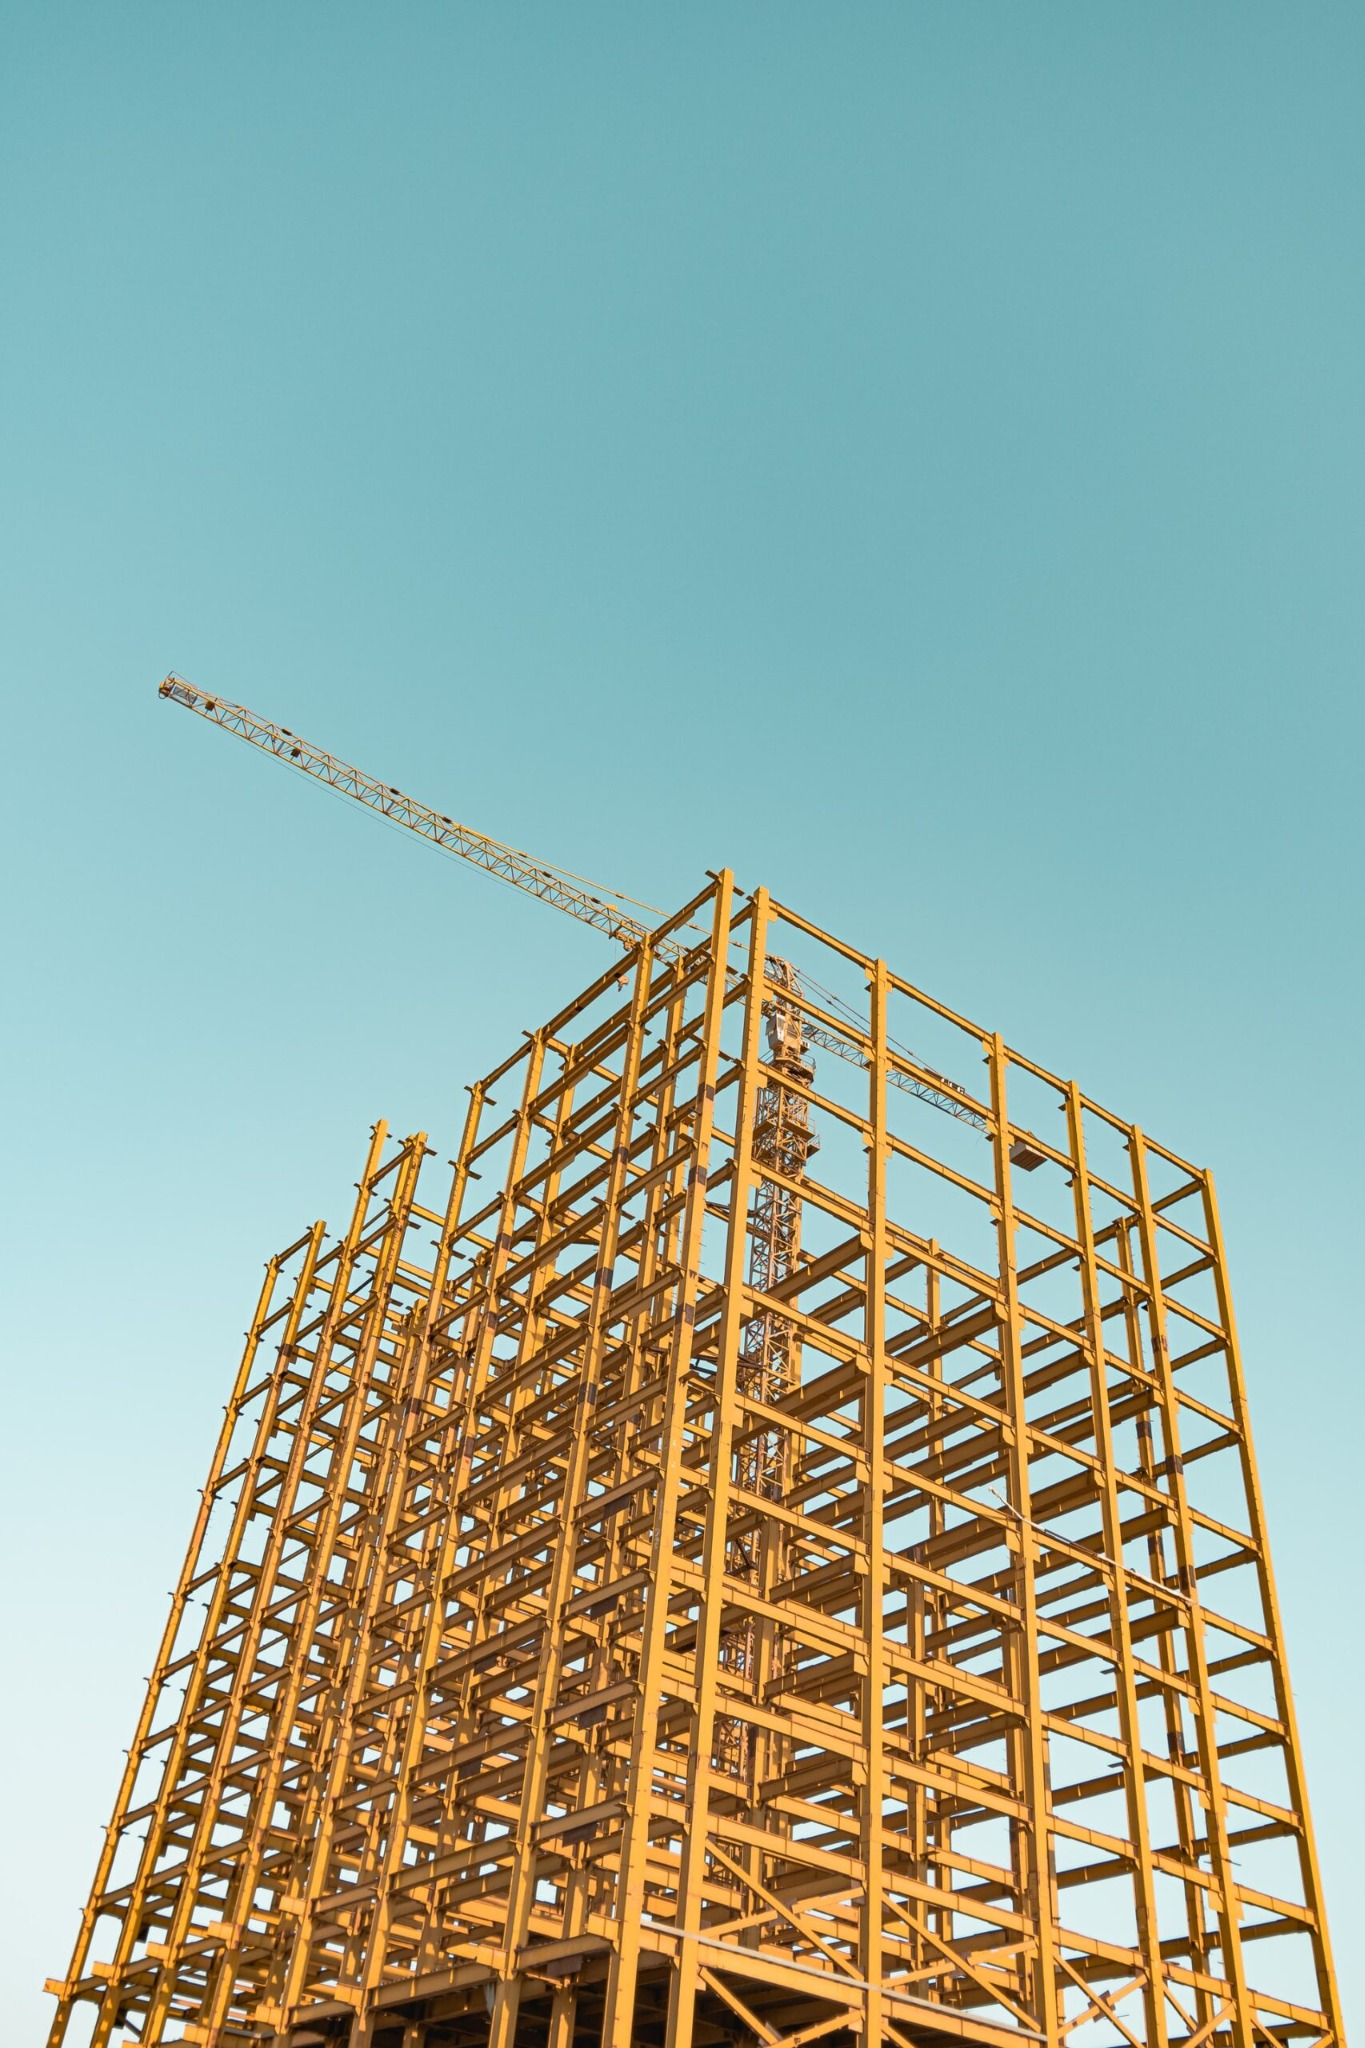
\includegraphics[
            height=\paperheight
        ]{../figures/cover.jpeg}
    };


    % ========================================================
    % 2. CABECERA SUPERIOR
    % ========================================================

    \path[
        fill=white,
        opacity=.88
    ]
        (current page.north west)
        rectangle ++(\paperwidth,-3.15cm);


    % Marca editorial
    \node[
        anchor=north west,
        xshift=1.8cm,
        yshift=-1.08cm,
        inner sep=0pt,
        text=coverNavy,
        font=\sffamily\bfseries\fontsize{18}{22}\selectfont
    ] at (current page.north west) {
        STUDIUM
    };


    % Línea de acento
    \node[
        anchor=north west,
        xshift=1.8cm,
        yshift=-2.17cm,
        inner sep=0pt
    ] at (current page.north west) {
        {\color{coverTeal}\rule{1.05cm}{2pt}}
    };


    % Colección
    \node[
        anchor=north west,
        xshift=3.15cm,
        yshift=-2.12cm,
        inner sep=0pt,
        text=coverNavy,
        font=\sffamily\fontsize{9}{12}\selectfont
    ] at (current page.north west) {
        BIBLIOTECA DE INGENIERÍA
    };


    % ========================================================
    % 3. BLOQUE INFERIOR
    % ========================================================

    \path[
        fill=coverNavy,
        opacity=.97
    ]
        (current page.south west)
        rectangle ++(\paperwidth,9.05cm);


    % Categoría
    \node[
        anchor=south west,
        xshift=1.8cm,
        yshift=8.13cm,
        inner sep=0pt,
        text=coverTeal,
        font=\sffamily\bfseries\fontsize{10}{13}\selectfont
    ] at (current page.south west) {
        MANUAL UNIVERSITARIO
    };


    % ========================================================
    % 4. TÍTULO PRINCIPAL
    % ========================================================

    \node[
        anchor=north west,
        xshift=1.8cm,
        yshift=7.42cm,
        inner sep=0pt,
        align=left,
        text=white,
        font=\rmfamily\bfseries\fontsize{35}{41}\selectfont
    ] at (current page.south west) {
        TEORÍA\\
        DE ESTRUCTURAS
    };


    % Subtítulo
    \node[
        anchor=west,
        xshift=1.8cm,
        yshift=3.88cm,
        inner sep=0pt,
        text=coverSoft,
        font=\sffamily\fontsize{11}{15}\selectfont
    ] at (current page.south west) {
        Fundamentos, análisis y problemas de ingeniería
    };


    % ========================================================
    % 5. INFORMACIÓN ACADÉMICA
    % ========================================================

    \node[
        anchor=west,
        xshift=1.8cm,
        yshift=3.03cm,
        inner sep=0pt,
        text=white,
        font=\sffamily\bfseries\fontsize{10}{13}\selectfont
    ] at (current page.south west) {
        GRADO EN INGENIERÍA AEROESPACIAL
    };


    \node[
        anchor=west,
        xshift=1.8cm,
        yshift=2.48cm,
        inner sep=0pt,
        text=coverSoft,
        font=\sffamily\fontsize{10}{13}\selectfont
    ] at (current page.south west) {
        Universidad de León
    };


    % ========================================================
    % 6. PIE EDITORIAL
    % ========================================================

    \node[
        anchor=south west,
        xshift=1.8cm,
        yshift=1.93cm,
        inner sep=0pt
    ] at (current page.south west) {
        {\color{coverSoft}\rule{15.5cm}{0.45pt}}
    };


    % Año
    \node[
        anchor=west,
        xshift=1.8cm,
        yshift=1.17cm,
        inner sep=0pt,
        text=coverSoft,
        font=\sffamily\fontsize{10}{13}\selectfont
    ] at (current page.south west) {
        2026
    };


    % Edición
    \node[
        anchor=east,
        xshift=-1.8cm,
        yshift=1.17cm,
        inner sep=0pt,
        text=white,
        font=\sffamily\bfseries\fontsize{10}{13}\selectfont
    ] at (current page.south east) {
        II Edición
    };

\end{tikzpicture}

\null
\clearpage

\chapter{Prefacio}
\noindent Este libro presenta el tema con el lenguaje del curso. Cada capítulo abre con una entrada breve, sigue con la explicación y cierra con un problema resuelto y una autoficha.
\chapter{Cómo usar este libro}
\noindent Lee el capítulo seguido. El consejo, la definición, el problema resuelto y la autoficha van en recuadros. La explicación es el cuerpo del texto.

\noindent Un capítulo lleva una entrada en cursiva, la explicación en el cuerpo, como mucho un consejo, definiciones solo al introducir un término, un problema resuelto y una autoficha.
\tableofcontents
\mainmatter

\part{Bloque I. Conceptos básicos}

\chapter{Introducción}
\label{chap:c01}

\noindent\textit{Este capítulo sitúa la asignatura. Describe qué es una estructura aeronáutica y de qué elementos se compone, qué materiales se emplean y por qué, y qué hipótesis permiten tratar el problema con las herramientas de la elasticidad lineal. Con ello se fija el lenguaje y el alcance de todo lo que sigue: una teoría de barras y de paredes delgadas que explique cómo se reparten las cargas, qué tensiones aparecen y cuánto se deforma la estructura.}

\begin{tcolorbox}[title={Autoficha}, studiumcheck, breakable]

¿Qué diferencia hay entre un monocasco y un semimonocasco, y por qué predomina el segundo en aviación comercial? ¿Qué elemento del ala soporta la mayor parte de la flexión y cuál mantiene el perfil aerodinámico? ¿Por qué un tirante de aluminio y otro de acero con la misma rigidez axial pesan prácticamente lo mismo? ¿Qué hipótesis adicionales, aparte de pequeños desplazamientos y linealidad, se admiten en el curso, y en qué se apoya el principio de superposición?
\end{tcolorbox}

\section{Estructuras aeronáuticas}

Una aeronave se descompone, desde el punto de vista estructural, en unos pocos elementos principales que trabajan juntos como un sistema integrado: el fuselaje, las alas, el empenaje y el tren de aterrizaje. Cada uno cumple una función propia, pero ninguno es independiente de los demás, porque las cargas que genera uno, sea la sustentación del ala, el peso de los depósitos o la reacción del tren en el aterrizaje, acaban transmitiéndose por los demás hasta equilibrarse. En el ala, la parte que soporta y reparte la carga es el cajón de torsión, o wingbox en inglés, que es la estructura principal del ala y el punto de unión de los demás componentes: flaps, bordes de ataque y extremos alares.

Dentro del ala conviene distinguir cuatro tipos de elementos. El revestimiento da forma al perfil aerodinámico, transmite a la estructura interna las presiones del aire y, además, trabaja: resiste las tensiones normales que produce la flexión y las tangenciales que produce el cortante y la torsión. Los largueros son las vigas principales del ala. Recorren el ala de la raíz a la punta y soportan la mayor parte de las cargas de flexión, mientras que el cortante y la torsión se reparten entre las almas de los largueros y el revestimiento. Entre las costillas y los largueros hay un reparto de papeles bien definido: el larguero lleva la carga a lo largo de la envergadura y la costilla la lleva desde el revestimiento hasta el larguero.

Las costillas son elementos transversales que determinan y mantienen el perfil aerodinámico, de modo que el revestimiento adopta la forma del perfil al tensarse sobre ellas. Los larguerillos son refuerzos longitudinales, más pequeños y más numerosos que los largueros, que se apoyan en las costillas y reducen la luz libre del revestimiento. Cuando se unen los largueros delantero y trasero con los revestimientos superior e inferior se forma una caja cerrada, el cajón de torsión. La figura~\ref{fig:c01-cajon} muestra una sección de un cajón de dos largueros con sus larguerillos.

\par\vspace{\baselineskip}
\noindent\begin{minipage}{\linewidth}
\centering
\begingroup
\setbox0=\hbox{\begin{tikzpicture}
\draw[thick] (0,0) -- (6,0.5) -- (6,2.2) -- (0,2.4) -- cycle;
\draw[very thick] (0,0) -- (0,2.4);
\draw[very thick] (6,0.5) -- (6,2.2);
\foreach \x/\yb/\yt in {1.2/0.1/2.3,2.4/0.2/2.3,3.6/0.3/2.25,4.8/0.4/2.25}{
  \fill (\x,\yb) rectangle ++(0.12,0.12);
  \fill (\x,\yt-0.12) rectangle ++(0.12,0.12);
}
\node[left] at (0,1.2) {larguero delantero};
\node[right] at (6,1.35) {larguero trasero};
\node[above] at (3,2.45) {revestimiento superior};
\node[below] at (3,0.05) {revestimiento inferior};
\node at (3,1.3) {cajón de torsión};
\draw[->] (3.6,0.6) -- (3.6,0.4) node[right,font=\small] {larguerillo};
\end{tikzpicture}}%
\count0=\ht0
\advance\count0 by \dp0
\count2=\wd0
\count4=\dimexpr\textheight/100*38\relax
\count6=\linewidth
\ifnum\count0<1
\count0=1
\fi
\ifnum\count2<1
\count2=1
\fi
\divide\count0 by 4096
\divide\count2 by 4096
\divide\count4 by 4096
\divide\count6 by 4096
\ifnum\count0<1
\count0=1
\fi
\ifnum\count2<1
\count2=1
\fi
\ifnum\count4<1
\count4=1
\fi
\ifnum\count6<1
\count6=1
\fi
\count8=\count2
\ifnum\count0>\count4
\count8=\numexpr\count2*\count4/\count0\relax
\fi
\ifnum\count8>\count6
\resizebox{\linewidth}{!}{\begin{tikzpicture}
\draw[thick] (0,0) -- (6,0.5) -- (6,2.2) -- (0,2.4) -- cycle;
\draw[very thick] (0,0) -- (0,2.4);
\draw[very thick] (6,0.5) -- (6,2.2);
\foreach \x/\yb/\yt in {1.2/0.1/2.3,2.4/0.2/2.3,3.6/0.3/2.25,4.8/0.4/2.25}{
  \fill (\x,\yb) rectangle ++(0.12,0.12);
  \fill (\x,\yt-0.12) rectangle ++(0.12,0.12);
}
\node[left] at (0,1.2) {larguero delantero};
\node[right] at (6,1.35) {larguero trasero};
\node[above] at (3,2.45) {revestimiento superior};
\node[below] at (3,0.05) {revestimiento inferior};
\node at (3,1.3) {cajón de torsión};
\draw[->] (3.6,0.6) -- (3.6,0.4) node[right,font=\small] {larguerillo};
\end{tikzpicture}}%
\else
\ifnum\count0>\count4
\resizebox{!}{\dimexpr\textheight/100*38\relax}{\begin{tikzpicture}
\draw[thick] (0,0) -- (6,0.5) -- (6,2.2) -- (0,2.4) -- cycle;
\draw[very thick] (0,0) -- (0,2.4);
\draw[very thick] (6,0.5) -- (6,2.2);
\foreach \x/\yb/\yt in {1.2/0.1/2.3,2.4/0.2/2.3,3.6/0.3/2.25,4.8/0.4/2.25}{
  \fill (\x,\yb) rectangle ++(0.12,0.12);
  \fill (\x,\yt-0.12) rectangle ++(0.12,0.12);
}
\node[left] at (0,1.2) {larguero delantero};
\node[right] at (6,1.35) {larguero trasero};
\node[above] at (3,2.45) {revestimiento superior};
\node[below] at (3,0.05) {revestimiento inferior};
\node at (3,1.3) {cajón de torsión};
\draw[->] (3.6,0.6) -- (3.6,0.4) node[right,font=\small] {larguerillo};
\end{tikzpicture}}%
\else
\begin{tikzpicture}
\draw[thick] (0,0) -- (6,0.5) -- (6,2.2) -- (0,2.4) -- cycle;
\draw[very thick] (0,0) -- (0,2.4);
\draw[very thick] (6,0.5) -- (6,2.2);
\foreach \x/\yb/\yt in {1.2/0.1/2.3,2.4/0.2/2.3,3.6/0.3/2.25,4.8/0.4/2.25}{
  \fill (\x,\yb) rectangle ++(0.12,0.12);
  \fill (\x,\yt-0.12) rectangle ++(0.12,0.12);
}
\node[left] at (0,1.2) {larguero delantero};
\node[right] at (6,1.35) {larguero trasero};
\node[above] at (3,2.45) {revestimiento superior};
\node[below] at (3,0.05) {revestimiento inferior};
\node at (3,1.3) {cajón de torsión};
\draw[->] (3.6,0.6) -- (3.6,0.4) node[right,font=\small] {larguerillo};
\end{tikzpicture}%
\fi
\fi
\endgroup
\par\nopagebreak
{\small \refstepcounter{studiumfigure}\label{fig:c01-cajon}\textbf{Figura~\thestudiumfigure.} Sección de un cajón de torsión de dos largueros: los revestimientos superior e inferior, con sus larguerillos, y las almas de los dos largueros forman una caja cerrada.\par}
\end{minipage}
\par\vspace{\baselineskip}

En el fuselaje se encuentran dos filosofías de construcción. En la estructura monocasco las cargas las soporta la piel exterior, de modo parecido a la cáscara de un huevo, y no hay una estructura interna que lleve carga. En un fuselaje real casi nunca se cumple del todo, porque una piel delgada sola pandea bajo compresión y no admite cargas concentradas. La solución habitual es la estructura semimonocasco, en la que un revestimiento resistente se combina con un armazón interno de cuadernas, larguerillos y mamparos. Esa es la estructura de la inmensa mayoría de los aviones grandes de transporte. El fuselaje debe resistir además la presurización y despresurización cíclicas de la cabina, que lo someten a fatiga, y la flexión vertical y horizontal en maniobra.

En un semimonocasco, las cuadernas son anillos transversales con la forma de la sección del fuselaje; mantienen esa forma y reparten las cargas; los larguerillos son elementos longitudinales ligeros que unen las cuadernas y llevan la carga axial de flexión; y el revestimiento de chapa, unido por remaches o adhesivos, cierra la superficie. Toda la carga de la presión interna la soporta el propio revestimiento como tensión de membrana. Que la piel trabaje es lo que hace que estas estructuras se llamen de revestimiento resistente, y por eso en este curso los revestimientos serán paredes delgadas que se estudian como tales en los temas 4 a 6. La figura~\ref{fig:c01-fuselaje} resume la disposición.

\par\vspace{\baselineskip}
\noindent\begin{minipage}{\linewidth}
\centering
\begingroup
\setbox0=\hbox{\begin{tikzpicture}
\draw[thick] (0,0) circle (2);
\draw[thick,dashed] (0,0) circle (1.75);
\foreach \a in {0,20,...,340}{
  \fill ({1.78*cos(\a)},{1.78*sin(\a)}) circle (0.05);
}
\draw[<-] (1.4,1.4) -- (2.6,2.3) node[right] {revestimiento};
\draw[<-] (0,-1.75) -- (0,-2.8) node[below] {cuaderna};
\draw[<-] ({1.78*cos(20)},{1.78*sin(20)}) -- (3.2,0.6) node[right] {larguerillo};
\draw[thick] (-1.75,-0.4) -- (1.75,-0.4);
\node at (0,-0.8) {suelo};
\end{tikzpicture}}%
\count0=\ht0
\advance\count0 by \dp0
\count2=\wd0
\count4=\dimexpr\textheight/100*38\relax
\count6=\linewidth
\ifnum\count0<1
\count0=1
\fi
\ifnum\count2<1
\count2=1
\fi
\divide\count0 by 4096
\divide\count2 by 4096
\divide\count4 by 4096
\divide\count6 by 4096
\ifnum\count0<1
\count0=1
\fi
\ifnum\count2<1
\count2=1
\fi
\ifnum\count4<1
\count4=1
\fi
\ifnum\count6<1
\count6=1
\fi
\count8=\count2
\ifnum\count0>\count4
\count8=\numexpr\count2*\count4/\count0\relax
\fi
\ifnum\count8>\count6
\resizebox{\linewidth}{!}{\begin{tikzpicture}
\draw[thick] (0,0) circle (2);
\draw[thick,dashed] (0,0) circle (1.75);
\foreach \a in {0,20,...,340}{
  \fill ({1.78*cos(\a)},{1.78*sin(\a)}) circle (0.05);
}
\draw[<-] (1.4,1.4) -- (2.6,2.3) node[right] {revestimiento};
\draw[<-] (0,-1.75) -- (0,-2.8) node[below] {cuaderna};
\draw[<-] ({1.78*cos(20)},{1.78*sin(20)}) -- (3.2,0.6) node[right] {larguerillo};
\draw[thick] (-1.75,-0.4) -- (1.75,-0.4);
\node at (0,-0.8) {suelo};
\end{tikzpicture}}%
\else
\ifnum\count0>\count4
\resizebox{!}{\dimexpr\textheight/100*38\relax}{\begin{tikzpicture}
\draw[thick] (0,0) circle (2);
\draw[thick,dashed] (0,0) circle (1.75);
\foreach \a in {0,20,...,340}{
  \fill ({1.78*cos(\a)},{1.78*sin(\a)}) circle (0.05);
}
\draw[<-] (1.4,1.4) -- (2.6,2.3) node[right] {revestimiento};
\draw[<-] (0,-1.75) -- (0,-2.8) node[below] {cuaderna};
\draw[<-] ({1.78*cos(20)},{1.78*sin(20)}) -- (3.2,0.6) node[right] {larguerillo};
\draw[thick] (-1.75,-0.4) -- (1.75,-0.4);
\node at (0,-0.8) {suelo};
\end{tikzpicture}}%
\else
\begin{tikzpicture}
\draw[thick] (0,0) circle (2);
\draw[thick,dashed] (0,0) circle (1.75);
\foreach \a in {0,20,...,340}{
  \fill ({1.78*cos(\a)},{1.78*sin(\a)}) circle (0.05);
}
\draw[<-] (1.4,1.4) -- (2.6,2.3) node[right] {revestimiento};
\draw[<-] (0,-1.75) -- (0,-2.8) node[below] {cuaderna};
\draw[<-] ({1.78*cos(20)},{1.78*sin(20)}) -- (3.2,0.6) node[right] {larguerillo};
\draw[thick] (-1.75,-0.4) -- (1.75,-0.4);
\node at (0,-0.8) {suelo};
\end{tikzpicture}%
\fi
\fi
\endgroup
\par\nopagebreak
{\small \refstepcounter{studiumfigure}\label{fig:c01-fuselaje}\textbf{Figura~\thestudiumfigure.} Sección de un fuselaje semimonocasco: el revestimiento, los larguerillos que lo rigidizan en dirección longitudinal y la cuaderna que mantiene la forma circular.\par}
\end{minipage}
\par\vspace{\baselineskip}

\begin{tcolorbox}[title={Consejo}, studiumtip, breakable]

Cuando veas un ala o un fuselaje, pregunta siempre qué carga lleva cada elemento. La respuesta típica es que los largueros y los cordones de larguerillos llevan tensión normal por flexión, y que las almas y los revestimientos llevan tensión tangencial por cortante y torsión. Esa separación de papeles es la base de la idealización de secciones que se estudiará en el tema 4.
\end{tcolorbox}

\section{Materiales}

El material estructural de la mayoría de las aeronaves de transporte ha sido, durante décadas, una aleación de aluminio. Las aleaciones de aluminio se usan en aviación por su alta relación resistencia-peso: el aluminio puro es demasiado blando, y alearlo con cobre, zinc, magnesio y otros elementos multiplica su resistencia. Sus módulos de elasticidad rondan los 70 GPa, aproximadamente un tercio del módulo de los aceros, de modo que, a igualdad de carga, una pieza de aluminio se deforma en régimen elástico más que una de acero de las mismas dimensiones. La aleación 7075, de la serie del zinc, tiene una densidad de \(2{,}81\) g/cm\(^3\), un módulo de Young de \(71{,}7\) GPa y un coeficiente de Poisson de \(0{,}33\); la 2024, la del cobre, tiene una densidad de \(2{,}78\) g/cm\(^3\) y un módulo de 73 GPa. Ambas se emplean mucho en elementos muy solicitados de aviones.

El titanio compite con el aluminio donde se necesita más resistencia a temperatura o menos volumen. La aleación Ti-6Al-4V, con un 6 \% de aluminio y un 4 \% de vanadio, es la más utilizada; es mucho más resistente que el titanio comercialmente puro, aunque tiene la misma rigidez. Para comparar materiales con distinta densidad se usa la rigidez específica \(E/\rho\), el módulo de Young dividido entre la densidad. Para el acero, con 200 GPa y unos \(7{,}9\) g/cm\(^3\), resulta un valor del orden de \(25\times 10^{6}\) m\(^2\)/s\(^2\), y las aleaciones de titanio, con un módulo de unos \(112{,}5\) GPa y una densidad de \(4{,}5\) g/cm\(^3\), dan el mismo orden de magnitud.

Los materiales compuestos se han incorporado a la estructura primaria de las aeronaves por su alta relación resistencia-peso y rigidez. En un plástico reforzado con fibra de carbono, las fibras aportan la rigidez y la resistencia, y una matriz polimérica, normalmente una resina termoestable como el epoxi, las mantiene unidas y transmite la carga entre ellas. Con una proporción de fibra y matriz de 70:30, unidireccional y en la dirección de las fibras, el módulo es de unos 181 GPa y la densidad de \(1{,}6\) g/cm\(^3\), lo que da una rigidez específica de \(113\times 10^{6}\) m\(^2\)/s\(^2\), más de cuatro veces la del acero. Esta ventaja solo existe en la dirección de las fibras; en las demás el material es mucho menos rígido y resistente, y por eso se dice que es anisótropo.

Veamos qué dice la rigidez específica con los datos anteriores. Para la aleación 7075, dividir \(71{,}7\times 10^{9}\) Pa entre 2810 kg/m\(^3\) da una rigidez específica de unos \(2{,}55\times 10^{7}\) m\(^2\)/s\(^2\); para un acero de 200 GPa y 7900 kg/m\(^3\) el valor es de unos \(2{,}53\times 10^{7}\) m\(^2\)/s\(^2\). Los dos valores son prácticamente iguales: un tirante de aluminio que deba tener la misma rigidez axial que otro de acero pesará lo mismo, aunque su sección sea casi tres veces mayor. Para el plástico reforzado con carbono, el cociente de \(181\times 10^{9}\) Pa entre 1600 kg/m\(^3\) da unos \(1{,}13\times 10^{8}\) m\(^2\)/s\(^2\), cuatro veces más. La razón es sencilla. Una barra prismática de longitud \(L\), sección \(A\) y módulo \(E\) tiene una rigidez axial
\begin{equation}
k = \frac{E\,A}{L}, \label{eq:c01-rigidez-axil}
\end{equation}
de modo que el área necesaria para una rigidez \(k\) dada es \(A = kL/E\) y la masa, que es la densidad por el volumen \(AL\), resulta
\begin{equation}
m = \frac{\rho\,k\,L^{2}}{E}. \label{eq:c01-masa-tirante}
\end{equation}
A rigidez \(k\) y longitud \(L\) fijas, la masa es proporcional a \(\rho/E\), es decir, inversamente proporcional a la rigidez específica.

Este criterio vale para elementos cuyo diseño lo manda la rigidez axial. Si lo manda la resistencia, hay que comparar las resistencias específicas, y si el elemento es una placa o una viga a flexión o a pandeo, el cociente que importa cambia de exponente: depende de \(E/\rho^{2}\) o de \(E/\rho^{3}\), según cómo pueda aumentarse el espesor. Por eso el aluminio sigue siendo competitivo en revestimientos, donde conviene un espesor mayor de un material ligero, y por eso la selección de material nunca se reduce a una sola propiedad. En lo que sigue se trabajará siempre con las propiedades elásticas de un material dado, y la elección del material será un dato del problema.

\begin{tcolorbox}[title={Definición}, studiumdef, breakable]

La rigidez específica de un material es el cociente entre su módulo de Young y su densidad, \(E/\rho\). Se expresa en m\(^2\)/s\(^2\) y mide cuánta rigidez axial se obtiene por unidad de masa.
\end{tcolorbox}

\section{Hipótesis básicas y sólidos elásticos}

La mecánica del sólido rígido estudia cuerpos indeformables, cuya forma y volumen permanecen constantes ante cualquier fuerza. Ese modelo basta para calcular las reacciones de una estructura, pero no dice nada de cómo se reparten las cargas dentro de ella. Para eso se necesita el modelo del sólido elástico, o deformable: un cuerpo que, ante una acción exterior, se deforma y que recupera su forma y su volumen originales cuando la acción desaparece. La tensión máxima que se puede alcanzar sin pasar a deformación plástica es el límite elástico; mientras no se rebase, la hipótesis es válida.

El comportamiento se supone además lineal, que en la teoría de la elasticidad lineal significa dos cosas: los desplazamientos y las deformaciones son pequeños, y la relación entre tensiones y deformaciones es lineal. Esta teoría solo es válida para estados de tensión que no produzcan fluencia, y sus hipótesis son razonables para muchos materiales de ingeniería y casos de diseño, de modo que se usa de forma extensa en el análisis estructural. A estas hipótesis básicas se añaden otras de carácter adicional: el material es homogéneo (sus propiedades no dependen del punto) e isótropo (no dependen de la orientación), el problema es estático e isotermo, y se admite el principio de Saint-Venant.

La isotropía es uniformidad en todas las orientaciones, y es la hipótesis que más conviene recordar cuando se trabaja con materiales compuestos. Las aleaciones metálicas usuales, con granos pequeños y orientados al azar, se tratan como isótropas; un laminado de fibra de carbono no, porque su módulo depende fuertemente de la dirección de las fibras. Los resultados de este curso se aplican por tanto sin cambios a las aleaciones de aluminio, de titanio y a los aceros, y se aplican a los materiales compuestos solo cuando se conoce su comportamiento en las direcciones de las fibras y se tiene en cuenta que cambia con ellas.

El principio de Saint-Venant afirma que la diferencia entre los efectos de dos cargas distintas, pero estáticamente equivalentes, es muy pequeña a distancias suficientemente grandes del punto de aplicación. Permite sustituir distribuciones de tensión complicadas, o condiciones de contorno difíciles de describir, por otras más sencillas, siempre que la frontera sea geométricamente pequeña. En la práctica significa que una carga puntual o un empotramiento mal definido solo perturban el estado de tensiones en un entorno de tamaño comparable a la dimensión de la sección, y que lejos de esa zona basta con conocer los esfuerzos resultantes, no cómo se aplican. Este principio es la justificación de que una barra pueda estudiarse con esfuerzos internos y no con tensiones puntuales.

Las hipótesis básicas, con deformaciones pequeñas y relación lineal entre tensiones y deformaciones, tienen dos consecuencias fundamentales. La primera es el principio de superposición: en un sistema lineal la respuesta neta a varias acciones es la suma de las respuestas a cada una por separado. Una viga, por ejemplo, puede modelarse como un sistema lineal cuya entrada es la carga y cuya salida es la flecha; así se puede calcular el efecto de un sistema de cargas complejo como suma de casos sencillos. La segunda consecuencia, que se enuncia en clase sin demostración, es la existencia y unicidad de la solución: con las hipótesis anteriores, cada problema bien planteado tiene una solución y solo una. De la unicidad se sigue que cualquier solución que cumpla equilibrio, compatibilidad y comportamiento es la solución, aunque se haya hallado por un camino distinto del estándar.

\begin{tcolorbox}[title={Consejo}, studiumtip, breakable]

La linealidad se pierde con rapidez cuando el material plastifica o cuando los giros dejan de ser pequeños. Antes de usar los métodos de los temas siguientes en un problema nuevo, conviene comprobar, aunque sea de forma aproximada, que la tensión máxima queda por debajo del límite elástico y que los desplazamientos son pequeños frente a las dimensiones del elemento.
\end{tcolorbox}

\begin{tcolorbox}[title={Derivaciones}, studiumdef, breakable]

\noindent\textbf{Masa de un tirante de rigidez axial dada}

\[
m = \frac{\rho\,k\,L^{2}}{E}
\]

\noindent\textbf{Hipótesis}
\begin{itemize}
\item barra prismática de material homogéneo
\item tracción uniforme: la rigidez axial es k = E A / L
\item la masa es densidad por volumen, \(m = \rho A L\)
\end{itemize}

\noindent\textbf{Limitaciones}
\begin{itemize}
\item no incluye uniones ni herrajes
\item solo vale si el diseño lo fija la rigidez y no la resistencia o el pandeo
\end{itemize}

\noindent\textbf{Pasos}
\begin{enumerate}
\item
despejar el área de la rigidez axial

\[
k = \frac{E A}{L} \;\Rightarrow\; A = \frac{k L}{E}
\]
\item
sustituir el área en la masa

\[
m = \rho\,A\,L = \frac{\rho\,k\,L^{2}}{E}
\]
\end{enumerate}

\noindent\textbf{Variables}
\begin{itemize}
\item $\rho$: densidad ($\mathrm{kg}\,\mathrm{m}^{-3}$)
\item $k$: rigidez axial ($\mathrm{N}\,\mathrm{m}^{-1}$)
\item $L$: longitud ($\mathrm{m}$)
\item $E$: módulo de Young ($\mathrm{Pa}$)
\end{itemize}

{\noindent\footnotesize verificada por comprobaciones independientes.\par}

\noindent\textbf{Rigidez axial de una barra prismática}

\[
k = \frac{E\,A}{L}
\]

\noindent\textbf{Hipótesis}
\begin{itemize}
\item barra prismática de material homogéneo, isótropo y elástico lineal
\item tensión uniforme en la sección
\end{itemize}

\noindent\textbf{Limitaciones}
\begin{itemize}
\item solo vale para barras prismáticas con tensión uniforme
\item lejos de los extremos cargados, por el principio de Saint-Venant
\end{itemize}

\noindent\textbf{Pasos}
\begin{enumerate}
\item
fuerza que ejerce la barra al alargarse

\[
F = \frac{E\,A\,\delta}{L}
\]
\item
la rigidez axial es la fuerza por unidad de alargamiento

\[
k = \frac{F}{\delta} = \frac{E\,A}{L}
\]
\end{enumerate}

\noindent\textbf{Variables}
\begin{itemize}
\item $E$: módulo de Young ($\mathrm{Pa}$)
\item $A$: área de la sección ($\mathrm{m}^{2}$)
\item $L$: longitud ($\mathrm{m}$)
\end{itemize}

{\noindent\footnotesize verificada por comprobaciones independientes.\par}
\end{tcolorbox}

\begin{tcolorbox}[title={Problema resuelto}, studiumworked, breakable]

\noindent\textbf{Enunciado}
Un tirante de 2 m de longitud debe tener una rigidez axial \(k = EA/L = 5\times 10^{7}\) N/m. Calcule su masa si es de aleación 7075 (\(E = 71{,}7\) GPa, \(\rho = 2810\) kg/m\(^3\)) y compare con la de un tirante de acero (\(E = 200\) GPa, \(\rho = 7900\) kg/m\(^3\)).

\noindent\textbf{Datos}
\begin{itemize}
\item $k = 50\,\mathrm{kN}\,\mathrm{mm}^{-1}$ — rigidez axial
\item $L = 2.0\,\mathrm{m}$ — longitud
\item $E = 71.7\,\mathrm{GPa}$ — módulo de Young del 7075
\item $\rho = 2810\,\mathrm{kg}\,\mathrm{m}^{-3}$ — densidad del 7075
\end{itemize}

\noindent\textbf{Incógnita}
masa del tirante de 7075

\noindent\textbf{Modelo físico}

\noindent\textit{Masa de un tirante de rigidez dada}

\[
m = \frac{\rho\,k\,L^{2}}{E}
\]

\noindent\textbf{Hipótesis}
\begin{itemize}
\item barra prismática y homogénea
\item diseño gobernado por la rigidez axial
\item no se incluyen uniones
\end{itemize}

\noindent\textbf{Desarrollo}
\begin{enumerate}
\item
Área necesaria con 7075
\item
Masa del tirante de acero, para comparar
\item
Masa del tirante de 7075, m = rho A L
\end{enumerate}

\noindent\textbf{Sustitución numérica}

\[
\frac{\left(2.0\,\mathrm{m}\right)^{2} \left(50\,\mathrm{kN}\,\mathrm{mm}^{-1}\right) \left(2810\,\mathrm{kg}\,\mathrm{m}^{-3}\right)}{\left(71.7\,\mathrm{GPa}\right)}
\]

\noindent\textbf{Resultado}

\[
m_{7075} \approx 7{,}84\ \mathrm{kg},\qquad m_{acero} = 7{,}90\ \mathrm{kg}
\]

\noindent\textbf{Interpretación}
Con igual rigidez axial, el tirante de aluminio pesa prácticamente lo mismo que el de acero, aunque su sección es casi tres veces mayor (\(13{,}9\) cm\(^2\) frente a \(5{,}0\) cm\(^2\)).

\noindent\textbf{Comprobación de los pasos}
\begin{itemize}
\item Paso 1: $0.0013947$ — reproducido
\item Paso 2: $7.9$ — reproducido
\item Paso 3: $7.83821$ — reproducido
\end{itemize}

\noindent\textbf{Comprobación de la respuesta} la aritmética del último paso reproduce la respuesta enunciada a la precisión con que está escrita. Es una reproducción aritmética; no valida el modelo físico ni sus hipótesis.

\noindent\textbf{Limitaciones}
\begin{itemize}
\item no considera la resistencia ni el pandeo
\item no incluye los herrajes de unión
\end{itemize}

\noindent\textbf{Errores frecuentes}
\begin{itemize}
\item usar la densidad en g/cm\(^3\) con el módulo en Pa sin convertir unidades
\item comparar solo los módulos de Young y no la masa
\end{itemize}
\end{tcolorbox}

\begin{tcolorbox}[title={Ejercicios}, studiumworked, breakable]

\noindent\textbf{1 (FOUNDATIONAL, NUMERICAL)}
Repita el cálculo del ejemplo para un tirante de plástico reforzado con fibra de carbono (\(E = 181\) GPa, \(\rho = 1600\) kg/m\(^3\), fibras en la dirección del tirante) con la misma rigidez axial \(k = 5\times 10^{7}\) N/m y longitud 2 m. Calcule su masa.

\noindent\textbf{2 (FOUNDATIONAL, NUMERICAL)}
Una aleación de titanio (\(E = 112{,}5\) GPa, \(\rho = 4500\) kg/m\(^3\)) se usa para un tirante de longitud 1 m con rigidez axial \(k = 2\times 10^{7}\) N/m. Calcule su masa.
\end{tcolorbox}

\chapter{Tensión y deformación}
\label{chap:c02}

\noindent\textit{Una estructura se carga y se deforma. Este capítulo introduce las dos magnitudes con las que se describe esa respuesta en cada punto del material, la tensión y la deformación, y la ley que las relaciona en el régimen elástico. Son las herramientas con las que, en los temas siguientes, se pasará de los esfuerzos que soporta una barra a las tensiones que sufre su material y a los desplazamientos que sufre la estructura.}

\begin{tcolorbox}[title={Autoficha}, studiumcheck, breakable]

¿Qué diferencia hay entre un esfuerzo y una tensión? ¿Cómo se descompone el vector tensión y qué signo tiene la tensión normal de tracción? ¿Qué plano de una barra traccionada soporta la tensión tangencial máxima y cuánto vale? ¿Qué relaciona el coeficiente de Poisson y por qué una barra traccionada adelgaza? ¿Qué zonas se distinguen en la curva tensión-deformación de un acero y en cuál es válida la ley de Hooke?
\end{tcolorbox}

\section{Concepto de tensión}

Cuando un cuerpo está cargado, cada parte de él ejerce fuerzas sobre las partes contiguas. Si se imagina un corte por una superficie de normal \(\mathbf{n}\), la parte situada a un lado ejerce sobre la otra una fuerza que se reparte sobre la superficie. La tensión se define como la fuerza que atraviesa una pequeña frontera por unidad de área de esa frontera, y se define para todas las orientaciones de la frontera. En el entorno de un punto, la fuerza \(\mathrm{d}\mathbf{F}\) que actúa sobre un elemento de área \(\mathrm{d}A_n\) define el vector tensión \(\mathbf{T}_n\) como el límite del cociente entre ambas cuando el elemento tiende a cero. Una tensión es siempre una fuerza por unidad de superficie y se expresa en pascales, o en MPa \(=\) N/mm\(^2\).

El vector tensión sobre una superficie puede tener cualquier dirección respecto a ella, y por eso se descompone en dos componentes: la tensión normal \(\sigma\), perpendicular a la superficie, y la tensión tangencial \(\tau\), contenida en ella. La tensión normal es positiva cuando la parte contigua tira del punto, es decir, cuando es de tracción, y negativa cuando empuja, es decir, de compresión. La tensión tangencial nace de la componente de la fuerza paralela al plano de corte, y la tensión normal de la perpendicular. Ese convenio, tracción positiva, es el que se usará siempre en el curso.

El caso más sencillo es una barra recta traccionada por una fuerza \(F\) aplicada en el centro de cada extremo. En una sección alejada de los extremos la tensión normal se reparte de manera uniforme y su valor es el cociente entre la fuerza y el área \(A\) de la sección,
\begin{equation}
\sigma = \frac{F}{A}. \label{eq:c02-sigma-media}
\end{equation}
Esta es la tensión media; en un punto cercano a una carga puntual la distribución real no es uniforme, y el principio de Saint-Venant dice que esa perturbación no llega lejos. Si la fuerza es paralela a la sección, la tensión tangencial media es también la fuerza dividida entre el área que la soporta. La tensión es un campo, es decir, varía de un punto a otro, y los esfuerzos internos de la barra no son más que las resultantes de las tensiones sobre una sección: la tensión normal da el axil y los flectores, y la tangencial el cortante y el torsor. Con ejes \(x\) a lo largo de la barra, \(y\) hacia abajo y \(z\) hacia el interior de la figura, esas resultantes son
\begin{equation}
N := \int_A \sigma_x\,\mathrm{d}A, \qquad M_z := \int_A y\,\sigma_x\,\mathrm{d}A, \qquad M_y := \int_A z\,\sigma_x\,\mathrm{d}A,
\end{equation}
\begin{equation}
C_y := \int_A \tau_{xy}\,\mathrm{d}A, \qquad C_z := \int_A \tau_{xz}\,\mathrm{d}A, \qquad M_x := \int_A \left(y\,\tau_{xz} - z\,\tau_{xy}\right)\mathrm{d}A.
\end{equation}
El primer subíndice de \(\tau\) indica la dirección normal al plano y el segundo la dirección de la tensión. Con estas definiciones \(M_z\) es positivo cuando traccionan las fibras de \(y\,>\,0\), que es lo mismo que decir que comprime las superiores.

La tensión en un punto depende del plano que se considere. Para verlo, se corta la barra traccionada con un plano cuya normal forma un ángulo \(\theta\) con el eje de la barra. El área de ese plano es \(A/\cos\theta\), la fuerza se descompone en una componente normal al plano, \(F\cos\theta\), y otra tangente a él, \(F\sin\theta\), y las tensiones sobre el plano valen
\begin{equation}
\sigma_{n} = \sigma\,\cos^{2}\theta, \qquad \tau_{\theta} = \sigma\,\sin\theta\,\cos\theta, \label{eq:c02-inclinado}
\end{equation}
donde \(\sigma = F/A\) es la tensión en la sección recta. La tensión normal es máxima en la sección recta, que es el plano de normal paralela al eje. La tensión tangencial se puede escribir también, con el ángulo doble,
\begin{equation}
\tau_{\theta} = \frac{1}{2}\,\sigma\,\sin 2\theta,
\end{equation}
de modo que se anula en la sección recta y alcanza su máximo a \(45^{\circ}\), donde vale la mitad de \(\sigma\). Esta es la razón por la que una probeta dúctil traccionada se desliza en planos inclinados unos \(45^{\circ}\) y por la que el criterio de Tresca, que se verá en el tema 8, se escribe con la tensión tangencial máxima. La figura~\ref{fig:c02-inclinado} muestra el equilibrio del trozo de barra.

\par\vspace{\baselineskip}
\noindent\begin{minipage}{\linewidth}
\centering
\begingroup
\setbox0=\hbox{\begin{tikzpicture}
\begin{scope}[scale=1.5,transform shape]
\draw[thick] (0,1.6) -- (3,1.6) -- (3,0) -- (0.92,0) -- cycle;
\draw[dashed] (-1.3,1.6) -- (0,1.6);
\draw[dashed] (-1.3,0) -- (0.92,0);
\draw[very thick,->] (3,0.8) -- (4.3,0.8) node[right] {$F$};
\coordinate (M) at (0.46,0.8);
\draw[very thick,->,red] (M) -- ++(-1.4,0) node[left] {$F$};
\draw[thick,->,blue] (M) -- ++(-1.048,-0.605) node[below left] {$F\cos\theta$};
\draw[thick,->,green!50!black] (M) -- ++(-0.35,0.606) node[above left] {$F\sin\theta$};
\draw[->] (0,1.0) arc (-90:-60:0.6);
\node at (0.3,0.82) {\small $\theta$};
\node at (2.0,0.8) {$A$};

\end{scope}
\end{tikzpicture}}%
\count0=\ht0
\advance\count0 by \dp0
\count2=\wd0
\count4=\dimexpr\textheight/100*38\relax
\count6=\linewidth
\ifnum\count0<1
\count0=1
\fi
\ifnum\count2<1
\count2=1
\fi
\divide\count0 by 4096
\divide\count2 by 4096
\divide\count4 by 4096
\divide\count6 by 4096
\ifnum\count0<1
\count0=1
\fi
\ifnum\count2<1
\count2=1
\fi
\ifnum\count4<1
\count4=1
\fi
\ifnum\count6<1
\count6=1
\fi
\count8=\count2
\ifnum\count0>\count4
\count8=\numexpr\count2*\count4/\count0\relax
\fi
\ifnum\count8>\count6
\resizebox{\linewidth}{!}{\begin{tikzpicture}
\begin{scope}[scale=1.5,transform shape]
\draw[thick] (0,1.6) -- (3,1.6) -- (3,0) -- (0.92,0) -- cycle;
\draw[dashed] (-1.3,1.6) -- (0,1.6);
\draw[dashed] (-1.3,0) -- (0.92,0);
\draw[very thick,->] (3,0.8) -- (4.3,0.8) node[right] {$F$};
\coordinate (M) at (0.46,0.8);
\draw[very thick,->,red] (M) -- ++(-1.4,0) node[left] {$F$};
\draw[thick,->,blue] (M) -- ++(-1.048,-0.605) node[below left] {$F\cos\theta$};
\draw[thick,->,green!50!black] (M) -- ++(-0.35,0.606) node[above left] {$F\sin\theta$};
\draw[->] (0,1.0) arc (-90:-60:0.6);
\node at (0.3,0.82) {\small $\theta$};
\node at (2.0,0.8) {$A$};

\end{scope}
\end{tikzpicture}}%
\else
\ifnum\count0>\count4
\resizebox{!}{\dimexpr\textheight/100*38\relax}{\begin{tikzpicture}
\begin{scope}[scale=1.5,transform shape]
\draw[thick] (0,1.6) -- (3,1.6) -- (3,0) -- (0.92,0) -- cycle;
\draw[dashed] (-1.3,1.6) -- (0,1.6);
\draw[dashed] (-1.3,0) -- (0.92,0);
\draw[very thick,->] (3,0.8) -- (4.3,0.8) node[right] {$F$};
\coordinate (M) at (0.46,0.8);
\draw[very thick,->,red] (M) -- ++(-1.4,0) node[left] {$F$};
\draw[thick,->,blue] (M) -- ++(-1.048,-0.605) node[below left] {$F\cos\theta$};
\draw[thick,->,green!50!black] (M) -- ++(-0.35,0.606) node[above left] {$F\sin\theta$};
\draw[->] (0,1.0) arc (-90:-60:0.6);
\node at (0.3,0.82) {\small $\theta$};
\node at (2.0,0.8) {$A$};

\end{scope}
\end{tikzpicture}}%
\else
\begin{tikzpicture}
\begin{scope}[scale=1.5,transform shape]
\draw[thick] (0,1.6) -- (3,1.6) -- (3,0) -- (0.92,0) -- cycle;
\draw[dashed] (-1.3,1.6) -- (0,1.6);
\draw[dashed] (-1.3,0) -- (0.92,0);
\draw[very thick,->] (3,0.8) -- (4.3,0.8) node[right] {$F$};
\coordinate (M) at (0.46,0.8);
\draw[very thick,->,red] (M) -- ++(-1.4,0) node[left] {$F$};
\draw[thick,->,blue] (M) -- ++(-1.048,-0.605) node[below left] {$F\cos\theta$};
\draw[thick,->,green!50!black] (M) -- ++(-0.35,0.606) node[above left] {$F\sin\theta$};
\draw[->] (0,1.0) arc (-90:-60:0.6);
\node at (0.3,0.82) {\small $\theta$};
\node at (2.0,0.8) {$A$};

\end{scope}
\end{tikzpicture}%
\fi
\fi
\endgroup
\par\nopagebreak
{\small \refstepcounter{studiumfigure}\label{fig:c02-inclinado}\textbf{Figura~\thestudiumfigure.} Equilibrio de un trozo de barra cortado por un plano que forma el ángulo \(\theta\) con la sección recta: la fuerza axial \(F\) se descompone en una componente normal \(F\cos\theta\) y otra tangencial \(F\sin\theta\) sobre el plano de área \(A/\cos\theta\).\par}
\end{minipage}
\par\vspace{\baselineskip}

\begin{tcolorbox}[title={Consejo}, studiumtip, breakable]

No confundas esfuerzo y tensión. El esfuerzo, como el axil \(N\), es una fuerza o un momento y se mide en N o N\(\cdot\)m; la tensión es una fuerza por unidad de área y se mide en Pa. Un esfuerzo es la resultante de una distribución de tensiones sobre toda la sección; una tensión es el valor de esa distribución en un punto.
\end{tcolorbox}

\begin{tcolorbox}[title={Definición}, studiumdef, breakable]

La tensión normal \(\sigma\) es la componente del vector tensión perpendicular al plano de corte y la tensión tangencial \(\tau\) es la componente contenida en él. Una y otra se miden en pascales; en estructuras se usa el megapascal, 1 MPa \(=\) 1 N/mm\(^2\). Aproximadamente, 1 MPa equivale a 10 kp/cm\(^2\), unidad que aparece en textos antiguos.
\end{tcolorbox}

\section{Concepto de deformación}

La deformación mide el cambio de forma de un cuerpo respecto de una configuración de referencia. Es una relación entre longitudes, de modo que es adimensional: se expresa como fracción decimal, como porcentaje o, para valores muy pequeños, en microdeformaciones. La definición más usual en estructuras es la deformación de ingeniería, adecuada para los materiales de la ingeniería mecánica y estructural, que sufren deformaciones muy pequeñas. En materiales como los elastómeros, que se deforman mucho, hacen falta otras definiciones.

Cuando un segmento de longitud inicial \(L\) cambia de longitud en \(\delta\), su deformación longitudinal es el alargamiento por unidad de longitud inicial,
\begin{equation}
\varepsilon := \frac{\delta}{L}, \label{eq:c02-eps}
\end{equation}
positiva si el material se alarga y negativa si se acorta. Además del cambio de longitud de las fibras, un elemento de material puede cambiar los ángulos que forman entre sí dos rectas inicialmente perpendiculares. Ese cambio angular, medido en radianes, es la deformación angular o distorsión \(\gamma\). El estado de deformación de un punto queda definido por las deformaciones longitudinales de todas las fibras que pasan por él y por las distorsiones de todos los pares de fibras perpendiculares; en los problemas de barras bastan las componentes en tres direcciones perpendiculares.

Una barra que se alarga en la dirección de la carga se contrae en las direcciones transversales. El cociente entre la deformación transversal y la axial, cambiado de signo, es el coeficiente de Poisson \(\nu\), de modo que
\begin{equation}
\varepsilon_{t} = -\nu\,\varepsilon_{a}, \label{eq:c02-poisson}
\end{equation}
con \(\varepsilon_{a}\) la deformación axial y \(\varepsilon_{t}\) la transversal. Muchos sólidos usuales tienen coeficientes de Poisson entre \(0{,}2\) y \(0{,}3\), y los aceros y los polímeros rígidos dentro de su rango de proyecto presentan valores en torno a \(0{,}3\). La aleación 7075 tiene \(\nu = 0{,}33\). Si se tira de una barra de 20 mm de diámetro hasta que se alarga el \(0{,}2\ \%\) de su longitud, el diámetro disminuye en \(\nu\,\varepsilon_{a}\,d\), es decir, unos 13 \(\mu\)m.

\begin{tcolorbox}[title={Consejo}, studiumtip, breakable]

Las deformaciones de las estructuras reales son pequeñas: una barra de acero que trabaja a 200 MPa se deforma el \(0{,}1\ \%\), es decir, \(0{,}001\) o 1000 microdeformaciones. Por eso se pueden suponer pequeñas deformaciones y usar la deformación de ingeniería, y por eso el cambio de sección que provoca el efecto Poisson es casi siempre despreciable en el cálculo de esfuerzos.
\end{tcolorbox}

\section{Leyes de comportamiento}

La ley de comportamiento relaciona tensión y deformación. La ley de Hooke, enunciada para un muelle como una fuerza proporcional al alargamiento, vale para una barra de material elástico lineal con pequeñas deformaciones: la tensión normal es proporcional a la deformación longitudinal, y la constante de proporcionalidad es el módulo de Young \(E\),
\begin{equation}
\sigma = E\,\varepsilon. \label{eq:c02-hooke}
\end{equation}
Aplicada a una barra de longitud \(L\) y sección \(A\), da la fuerza que ejerce la barra al alargarse, \(F = E\,A\,\delta/L\), de modo que la barra se comporta como un muelle de rigidez \(EA/L\), como se vio en el capítulo 1. En cortadura la ley es análoga: la tensión tangencial es proporcional a la distorsión, con el módulo transversal \(G\) como constante, y para un material isótropo \(G\) no es independiente de \(E\) y \(\nu\).

El módulo transversal se define como la razón entre la tensión tangencial y la distorsión, \(G := \tau/\gamma\), y en un material isótropo vale
\begin{equation}
G = \frac{E}{2\,(1+\nu)}. \label{eq:c02-G}
\end{equation}
Para la aleación 7075, con \(E = 71{,}7\) GPa y \(\nu = 0{,}33\), el módulo transversal es de unos \(26{,}95\) GPa, y bajo una tensión tangencial de 50 MPa la distorsión es de unos \(1{,}855\times 10^{-3}\) rad, es decir, menos de una décima de grado. Que dos constantes basten, \(E\) y \(\nu\), para describir el comportamiento elástico de un material isótropo se demostrará en el tema 8.

La ley de Hooke solo es válida en una parte de la curva tensión-deformación, que se obtiene con un ensayo de tracción. En la primera zona, elástica, la tensión es proporcional a la deformación y la pendiente es el módulo de Young; el material solo sufre deformación elástica y recupera su forma al descargar. El final de ese tramo marca el comienzo de la deformación plástica, y la tensión en ese punto es el límite elástico o tensión de fluencia, que es la que se usa como tensión admisible de referencia. Una vez rebasada, una parte de la deformación es permanente y no se recupera. En los aceros dulces se distinguen además el límite de linealidad, ligeramente por debajo del elástico, y una meseta de fluencia.

Tras la fluencia viene la zona de endurecimiento, en la que la tensión vuelve a crecer con la deformación hasta un máximo, la tensión última o resistencia a tracción. Más allá, en la zona de estricción, la sección de la probeta se reduce localmente, la deformación se concentra en ese punto y lleva a la rotura. La tensión de ingeniería baja en esta zona porque se calcula sobre la sección inicial, no sobre la que realmente queda, aunque la tensión verdadera siga creciendo. La figura~\ref{fig:c02-curva} resume las zonas de la curva de un acero. En el curso solo se usa la zona elástica, y el resto sirve para saber hasta dónde se puede apurar el material.

\par\vspace{\baselineskip}
\noindent\begin{minipage}{\linewidth}
\centering
\begingroup
\setbox0=\hbox{\begin{tikzpicture}
\draw[->] (0,0) -- (7.6,0) node[right] {$\varepsilon$};
\draw[->] (0,0) -- (0,4.6) node[above] {$\sigma$};
\draw[very thick] (0,0) -- (1.3,2.6) -- (1.5,2.7) -- (2.4,2.6) .. controls (3.4,2.7) and (4.8,4.1) .. (5.4,4.2) .. controls (6.2,4.2) and (6.6,3.4) .. (7,2.9);
\draw[dashed] (1.3,0) -- (1.3,2.6);
\draw[dashed] (5.4,0) -- (5.4,4.2);
\draw[dashed] (0,2.7) -- (1.5,2.7);
\draw[dashed] (0,4.2) -- (5.4,4.2);
\node[left] at (0,2.7) {$\sigma_{e}$};
\node[left] at (0,4.2) {$\sigma_{u}$};
\node[below] at (0.7,0) {\small elástica};
\node[below] at (1.9,0) {\small fluencia};
\node[below] at (3.9,0) {\small endurecimiento};
\node[below] at (6.4,0) {\small estricción};
\node[right] at (7,2.9) {rotura};
\end{tikzpicture}}%
\count0=\ht0
\advance\count0 by \dp0
\count2=\wd0
\count4=\dimexpr\textheight/100*38\relax
\count6=\linewidth
\ifnum\count0<1
\count0=1
\fi
\ifnum\count2<1
\count2=1
\fi
\divide\count0 by 4096
\divide\count2 by 4096
\divide\count4 by 4096
\divide\count6 by 4096
\ifnum\count0<1
\count0=1
\fi
\ifnum\count2<1
\count2=1
\fi
\ifnum\count4<1
\count4=1
\fi
\ifnum\count6<1
\count6=1
\fi
\count8=\count2
\ifnum\count0>\count4
\count8=\numexpr\count2*\count4/\count0\relax
\fi
\ifnum\count8>\count6
\resizebox{\linewidth}{!}{\begin{tikzpicture}
\draw[->] (0,0) -- (7.6,0) node[right] {$\varepsilon$};
\draw[->] (0,0) -- (0,4.6) node[above] {$\sigma$};
\draw[very thick] (0,0) -- (1.3,2.6) -- (1.5,2.7) -- (2.4,2.6) .. controls (3.4,2.7) and (4.8,4.1) .. (5.4,4.2) .. controls (6.2,4.2) and (6.6,3.4) .. (7,2.9);
\draw[dashed] (1.3,0) -- (1.3,2.6);
\draw[dashed] (5.4,0) -- (5.4,4.2);
\draw[dashed] (0,2.7) -- (1.5,2.7);
\draw[dashed] (0,4.2) -- (5.4,4.2);
\node[left] at (0,2.7) {$\sigma_{e}$};
\node[left] at (0,4.2) {$\sigma_{u}$};
\node[below] at (0.7,0) {\small elástica};
\node[below] at (1.9,0) {\small fluencia};
\node[below] at (3.9,0) {\small endurecimiento};
\node[below] at (6.4,0) {\small estricción};
\node[right] at (7,2.9) {rotura};
\end{tikzpicture}}%
\else
\ifnum\count0>\count4
\resizebox{!}{\dimexpr\textheight/100*38\relax}{\begin{tikzpicture}
\draw[->] (0,0) -- (7.6,0) node[right] {$\varepsilon$};
\draw[->] (0,0) -- (0,4.6) node[above] {$\sigma$};
\draw[very thick] (0,0) -- (1.3,2.6) -- (1.5,2.7) -- (2.4,2.6) .. controls (3.4,2.7) and (4.8,4.1) .. (5.4,4.2) .. controls (6.2,4.2) and (6.6,3.4) .. (7,2.9);
\draw[dashed] (1.3,0) -- (1.3,2.6);
\draw[dashed] (5.4,0) -- (5.4,4.2);
\draw[dashed] (0,2.7) -- (1.5,2.7);
\draw[dashed] (0,4.2) -- (5.4,4.2);
\node[left] at (0,2.7) {$\sigma_{e}$};
\node[left] at (0,4.2) {$\sigma_{u}$};
\node[below] at (0.7,0) {\small elástica};
\node[below] at (1.9,0) {\small fluencia};
\node[below] at (3.9,0) {\small endurecimiento};
\node[below] at (6.4,0) {\small estricción};
\node[right] at (7,2.9) {rotura};
\end{tikzpicture}}%
\else
\begin{tikzpicture}
\draw[->] (0,0) -- (7.6,0) node[right] {$\varepsilon$};
\draw[->] (0,0) -- (0,4.6) node[above] {$\sigma$};
\draw[very thick] (0,0) -- (1.3,2.6) -- (1.5,2.7) -- (2.4,2.6) .. controls (3.4,2.7) and (4.8,4.1) .. (5.4,4.2) .. controls (6.2,4.2) and (6.6,3.4) .. (7,2.9);
\draw[dashed] (1.3,0) -- (1.3,2.6);
\draw[dashed] (5.4,0) -- (5.4,4.2);
\draw[dashed] (0,2.7) -- (1.5,2.7);
\draw[dashed] (0,4.2) -- (5.4,4.2);
\node[left] at (0,2.7) {$\sigma_{e}$};
\node[left] at (0,4.2) {$\sigma_{u}$};
\node[below] at (0.7,0) {\small elástica};
\node[below] at (1.9,0) {\small fluencia};
\node[below] at (3.9,0) {\small endurecimiento};
\node[below] at (6.4,0) {\small estricción};
\node[right] at (7,2.9) {rotura};
\end{tikzpicture}%
\fi
\fi
\endgroup
\par\nopagebreak
{\small \refstepcounter{studiumfigure}\label{fig:c02-curva}\textbf{Figura~\thestudiumfigure.} Curva tensión-deformación de un acero dulce con sus zonas: elástica (hasta el límite elástico), de fluencia, de endurecimiento y de estricción, que acaba en la rotura.\par}
\end{minipage}
\par\vspace{\baselineskip}

Los materiales se clasifican según lo que ocurre después del límite elástico. Un material dúctil soporta una deformación plástica importante antes de romper y avisa, porque se deforma mucho antes de fallar; la tensión última puede ser bastante mayor que el límite elástico. Un material frágil rompe con poca o ninguna deformación plástica y absorbe poca energía antes de la rotura, incluso aunque sea resistente; en ellos la tensión última está cerca del límite elástico. Las aleaciones de aluminio de uso aeronáutico son dúctiles. El 7075 en temple T6 tiene una tensión última de 510 a 540 MPa y un alargamiento de rotura de 5 a \(11\ \%\). En proyecto se exige que la tensión máxima de servicio quede muy por debajo del límite elástico, con un coeficiente de seguridad, y esa es la comprobación de resistencia que se hace al final de cada problema de barras.

\begin{tcolorbox}[title={Derivaciones}, studiumdef, breakable]

\noindent\textbf{Tensión media en una barra traccionada}

\[
\sigma = \frac{F}{A}
\]

\noindent\textbf{Hipótesis}
\begin{itemize}
\item fuerza axial centrada en la sección
\item sección alejada de los extremos cargados (Saint-Venant)
\item tensión normal uniforme
\end{itemize}

\noindent\textbf{Limitaciones}
\begin{itemize}
\item solo es la tensión media; cerca de las cargas puntuales la distribución no es uniforme
\end{itemize}

\noindent\textbf{Pasos}
\begin{enumerate}
\item
la tensión es la fuerza por unidad de área

\[
\mathrm{d}F = \sigma\,\mathrm{d}A
\]
\item
con tensión uniforme la resultante es tensión por área

\[
F = \sigma\,A \;\Rightarrow\; \sigma = \frac{F}{A}
\]
\end{enumerate}

\noindent\textbf{Variables}
\begin{itemize}
\item $F$: fuerza axial ($\mathrm{N}$)
\item $A$: área de la sección ($\mathrm{m}^{2}$)
\item $\sigma$: tensión normal ($\mathrm{Pa}$)
\end{itemize}

{\noindent\footnotesize verificada por comprobaciones independientes.\par}

\noindent\textbf{Tensión normal en un plano inclinado}

\begin{equation}
\sigma_{n} = \sigma\,\cos^{2}\theta
\label{eq:c02-inclinado-normal}
\end{equation}

\noindent\textbf{Hipótesis}
\begin{itemize}
\item barra de sección A con tensión uniforme \(\sigma = F/A\)
\item el plano forma el ángulo \(\theta\) con la sección recta
\end{itemize}

\noindent\textbf{Limitaciones}
\begin{itemize}
\item se supone carga axial centrada y tensión uniforme
\end{itemize}

\noindent\textbf{Pasos}
\begin{enumerate}
\item
el área del plano inclinado es \(A/cos \theta\)

\[
A_{\theta} = \frac{A}{\cos\theta}
\]
\item
la componente normal de la fuerza es F cos \(\theta\)

\[
F_{n} = F\cos\theta
\]
\item
dividir una entre otra

\[
\sigma_{n} = \frac{F\cos\theta}{A/\cos\theta} = \frac{F}{A}\cos^{2}\theta
\]
\end{enumerate}

\noindent\textbf{Variables}
\begin{itemize}
\item $\sigma$: tensión en la sección recta ($\mathrm{Pa}$)
\item $\sigma_{n}$: tensión normal en el plano inclinado ($\mathrm{Pa}$)
\item $\theta$: ángulo del plano ($\mathrm{rad}$)
\end{itemize}

{\noindent\footnotesize verificada por comprobaciones independientes.\par}

\noindent\textbf{Tensión tangencial en un plano inclinado}

\begin{equation}
\tau_{\theta} = \sigma\,\sin\theta\,\cos\theta
\label{eq:c02-inclinado-tangencial}
\end{equation}

\noindent\textbf{Hipótesis}
\begin{itemize}
\item barra de sección A con tensión uniforme \(\sigma = F/A\)
\item se toma el módulo de la tensión tangencial
\end{itemize}

\noindent\textbf{Limitaciones}
\begin{itemize}
\item módulo de la tensión tangencial; el sentido lo da el sentido de la componente de la fuerza en el plano
\end{itemize}

\noindent\textbf{Pasos}
\begin{enumerate}
\item
la componente de la fuerza en el plano es F sin \(\theta\)

\[
F_{t} = F\sin\theta
\]
\item
dividir entre el área \(A/cos \theta\) del plano

\[
\tau_{\theta} = \frac{F\sin\theta}{A/\cos\theta} = \frac{F}{A}\sin\theta\cos\theta
\]
\end{enumerate}

\noindent\textbf{Variables}
\begin{itemize}
\item $\sigma$: tensión en la sección recta ($\mathrm{Pa}$)
\item $\tau_{\theta}$: tensión tangencial en el plano inclinado ($\mathrm{Pa}$)
\item $\theta$: ángulo del plano ($\mathrm{rad}$)
\end{itemize}

{\noindent\footnotesize verificada por comprobaciones independientes.\par}

\noindent\textbf{Tensión tangencial en un plano inclinado, con el ángulo doble}

\begin{equation}
\tau_{\theta} = \frac{1}{2}\,\sigma\,\sin 2\theta
\label{eq:c02-tau-doble}
\end{equation}

\noindent\textbf{Hipótesis}
\begin{itemize}
\item tracción uniaxial uniforme
\item sin \(2\theta = 2\) sin \(\theta\) cos \(\theta\)
\end{itemize}

\noindent\textbf{Limitaciones}
\begin{itemize}
\item módulo de la tensión tangencial
\end{itemize}

\noindent\textbf{Pasos}
\begin{enumerate}
\item
partir de la tensión tangencial sobre el plano inclinado

\[
\tau_{\theta} = \sigma\,\sin\theta\,\cos\theta
\]
\item
aplicar la fórmula del ángulo doble

\[
\sin 2\theta = 2\sin\theta\cos\theta \;\Rightarrow\; \tau_{\theta} = \frac{1}{2}\,\sigma\,\sin 2\theta
\]
\end{enumerate}

\noindent\textbf{Variables}
\begin{itemize}
\item $\sigma$: tensión en la sección recta ($\mathrm{Pa}$)
\item $\tau_{\theta}$: tensión tangencial en el plano inclinado ($\mathrm{Pa}$)
\item $\theta$: ángulo del plano ($\mathrm{rad}$)
\end{itemize}

{\noindent\footnotesize verificada por comprobaciones independientes.\par}

\noindent\textbf{Fuerza de una barra en función de su alargamiento}

\begin{equation}
F = \frac{E\,A\,\delta}{L}
\label{eq:c02-fuerza-alargamiento}
\end{equation}

\noindent\textbf{Hipótesis}
\begin{itemize}
\item barra prismática de material elástico lineal
\item tensión uniforme
\end{itemize}

\noindent\textbf{Limitaciones}
\begin{itemize}
\item barra prismática con tensión uniforme
\end{itemize}

\noindent\textbf{Pasos}
\begin{enumerate}
\item
tensión media y ley de Hooke

\[
\sigma = \frac{F}{A}, \qquad \sigma = E\,\varepsilon
\]
\item
deformación de la barra

\[
\varepsilon = \frac{\delta}{L}
\]
\item
despejar la fuerza

\[
F = \sigma\,A = \frac{E\,A\,\delta}{L}
\]
\end{enumerate}

\noindent\textbf{Variables}
\begin{itemize}
\item $E$: módulo de Young ($\mathrm{Pa}$)
\item $A$: área de la sección ($\mathrm{m}^{2}$)
\item $\delta$: alargamiento ($\mathrm{m}$)
\item $L$: longitud ($\mathrm{m}$)
\item $F$: fuerza axial ($\mathrm{N}$)
\end{itemize}

{\noindent\footnotesize verificada por comprobaciones independientes.\par}

\noindent\textbf{Ley de Hooke uniaxial}

\[
\sigma = E\,\varepsilon
\]

\noindent\textbf{Hipótesis}
\begin{itemize}
\item material elástico lineal
\item tensión uniaxial
\item deformaciones pequeñas
\end{itemize}

\noindent\textbf{Limitaciones}
\begin{itemize}
\item solo vale en el tramo lineal de la curva tensión-deformación
\end{itemize}

\noindent\textbf{Pasos}
\begin{enumerate}
\item
el módulo de Young es la razón entre tensión y deformación

\[
E = \frac{\sigma}{\varepsilon}
\]
\item
despejar la tensión

\[
\sigma = E\,\varepsilon
\]
\end{enumerate}

\noindent\textbf{Variables}
\begin{itemize}
\item $E$: módulo de Young ($\mathrm{Pa}$)
\item $\varepsilon$: deformación longitudinal
\item $\sigma$: tensión normal ($\mathrm{Pa}$)
\end{itemize}

{\noindent\footnotesize verificada por comprobaciones independientes.\par}

\noindent\textbf{Deformación transversal por efecto Poisson}

\[
\varepsilon_{t} = -\nu\,\varepsilon_{a}
\]

\noindent\textbf{Hipótesis}
\begin{itemize}
\item material isótropo y elástico lineal
\item carga uniaxial
\end{itemize}

\noindent\textbf{Limitaciones}
\begin{itemize}
\item solo en el tramo elástico lineal
\end{itemize}

\noindent\textbf{Pasos}
\begin{enumerate}
\item
el coeficiente de Poisson es el cociente cambiado de signo entre deformación transversal y axial

\[
\nu = -\frac{\varepsilon_{t}}{\varepsilon_{a}}
\]
\item
despejar la deformación transversal

\[
\varepsilon_{t} = -\nu\,\varepsilon_{a}
\]
\end{enumerate}

\noindent\textbf{Variables}
\begin{itemize}
\item $\epsilon_{t}$: deformación transversal
\item $\epsilon_{a}$: deformación axial
\item $\nu$: coeficiente de Poisson
\end{itemize}

{\noindent\footnotesize verificada por comprobaciones independientes.\par}
\end{tcolorbox}

\begin{tcolorbox}[title={Problema resuelto}, studiumworked, breakable]

\noindent\textbf{Enunciado}
Una barra de aleación 7075 (\(E = 71{,}7\) GPa) de 20 mm de diámetro y \(1{,}5\) m de longitud soporta una tracción axial de 60 kN. Calcule la tensión normal, la deformación y el alargamiento total, y compruebe que la tensión queda por debajo del límite elástico mínimo de 430 MPa.

\noindent\textbf{Datos}
\begin{itemize}
\item $F = 60000\,\mathrm{N}$ — tracción axial
\item $d = 0.02\,\mathrm{m}$ — diámetro
\item $L = 1.5\,\mathrm{m}$ — longitud
\item $E = 71.7\,\mathrm{GPa}$ — módulo de Young del 7075
\end{itemize}

\noindent\textbf{Incógnita}
alargamiento total de la barra

\noindent\textbf{Modelo físico}

\noindent\textit{Alargamiento de una barra traccionada}

\[
\delta = \frac{F\,L}{E\,A},\quad A = \frac{\pi d^{2}}{4}
\]

\noindent\textbf{Hipótesis}
\begin{itemize}
\item tensión uniforme lejos de los extremos
\item material elástico lineal
\item pequeñas deformaciones
\end{itemize}

\noindent\textbf{Desarrollo}
\begin{enumerate}
\item
Área de la sección
\item
Tensión normal sigma = F/A
\item
Deformación epsilon = sigma/E
\item
Coeficiente de seguridad respecto al límite elástico
\item
Alargamiento total delta = epsilon L
\end{enumerate}

\noindent\textbf{Sustitución numérica}

\[
\frac{4 \left(60000\,\mathrm{N}\right) \left(1.5\,\mathrm{m}\right)}{\pi \left(71.7\,\mathrm{GPa}\right) \left(0.02\,\mathrm{m}\right)^{2}}
\]

\noindent\textbf{Resultado}

\[
\sigma \approx 191\ \mathrm{MPa},\quad \varepsilon \approx 2{,}66\times 10^{-3},\quad \delta \approx 4{,}00\ \mathrm{mm}
\]

\noindent\textbf{Interpretación}
La tensión es menos de la mitad del límite elástico mínimo (coeficiente de seguridad \(2{,}25\)) y la barra trabaja en el tramo lineal; el alargamiento de 4 mm en 1,5 m es una deformación del \(0{,}27\ \%\).

\noindent\textbf{Comprobación de los pasos}
\begin{itemize}
\item Paso 1: $0.000314159$ — reproducido
\item Paso 2: $190.986$ — reproducido
\item Paso 3: $0.00266368$ — reproducido
\item Paso 4: $2.25147$ — reproducido
\item Paso 5: $3.99552$ — reproducido
\end{itemize}

\noindent\textbf{Comprobación de la respuesta} la aritmética del último paso reproduce la respuesta enunciada a la precisión con que está escrita. Es una reproducción aritmética; no valida el modelo físico ni sus hipótesis.

\noindent\textbf{Limitaciones}
\begin{itemize}
\item no se incluye la reducción de diámetro por efecto Poisson
\item no se consideran las uniones de los extremos
\end{itemize}

\noindent\textbf{Errores frecuentes}
\begin{itemize}
\item usar milímetros y newtons sin convertir el módulo de Young a MPa
\item usar el diámetro en lugar del área
\end{itemize}
\end{tcolorbox}

\begin{tcolorbox}[title={Ejercicios}, studiumworked, breakable]

\noindent\textbf{1 (FOUNDATIONAL, NUMERICAL)}
La barra del ejemplo anterior (diámetro 20 mm, \(\nu = 0{,}33\)) se alarga una deformación axial de \(2{,}0\times 10^{-3}\). Calcule la disminución de su diámetro, en milímetros.

\noindent\textbf{2 (INTERMEDIATE, MULTI\_STEP)}
Una chapa de 7075 (\(E = 71{,}7\) GPa, \(\nu = 0{,}33\)) trabaja a cortadura pura con una tensión tangencial de 50 MPa. Calcule el módulo transversal \(G\) y la distorsión \(\gamma\).

\noindent\textbf{3 (FOUNDATIONAL, NUMERICAL)}
Una barra soporta una tensión normal \(\sigma = 100\) MPa en su sección recta. Calcule la tensión normal sobre un plano cuya normal forma \(30^{\circ}\) con el eje de la barra.

\noindent\textbf{4 (INTERMEDIATE, NUMERICAL)}
En una barra con \(\sigma = 100\) MPa en la sección recta, calcule la tensión tangencial máxima y el ángulo \(\theta\) del plano en que se produce.
\end{tcolorbox}

\chapter{Modelo monodimensional}
\label{chap:c03}

\noindent\textit{Calcular una estructura real exige primero idealizarla. Este capítulo construye el modelo monodimensional con el que se resolverá casi todo el curso: la barra como una línea con una sección asociada, las cargas y los apoyos que actúan sobre ella, el equilibrio que determina las reacciones y, por último, los esfuerzos internos y las leyes que los describen a lo largo de la barra.}

\begin{tcolorbox}[title={Autoficha}, studiumcheck, breakable]

¿Qué es la directriz y qué es una rebanada? ¿Qué tres ecuaciones de equilibrio hay en el plano y cuántas reacciones se pueden calcular con ellas? ¿Qué distingue una estructura isostática de una hiperestática? ¿Cómo es el signo de un cortante positivo, de un flector positivo y de un torsor positivo? ¿Qué relación hay entre la pendiente del diagrama de flectores y el cortante, y entre la del cortante y la carga? ¿Dónde está el máximo del flector de una viga con carga repartida?
\end{tcolorbox}

\section{Modelización y secciones}

El modelo estructural es una idealización de la estructura real. Una viga es un elemento estructural que soporta cargas perpendiculares a su eje largo, y su modo principal de deformación es la flexión: las cargas producen reacciones en los apoyos y, en el interior, momentos flectores, cortantes, tensiones, deformaciones y flechas. Para calcularla se sustituye por su directriz, la línea que une los centros de gravedad de sus secciones, a la que se asocia en cada punto la sección transversal con sus propiedades. El sentido de avance a lo largo de la directriz define qué cara de cada corte es la frontal y cuál la dorsal. Una rebanada es la porción de barra comprendida entre dos secciones infinitamente próximas. La teoría de vigas de Euler-Bernoulli, en la que se basa este curso, se limita a pequeñas flechas bajo cargas laterales que producen flexión elástica.

Los ejes de la sección se toman con origen en su centro de gravedad. El eje \(x\) va a lo largo de la directriz, el eje \(y\) está contenido en la sección y apunta hacia abajo, y el eje \(z\) completa un triedro directo; en un alzado con \(x\) hacia la derecha, el eje \(z\) entra en el papel. El área y la posición del centro de gravedad se obtienen de las integrales de superficie,
\begin{equation}
A := \int_A \mathrm{d}A, \qquad y_G := \frac{1}{A}\int_A y\,\mathrm{d}A, \qquad z_G := \frac{1}{A}\int_A z\,\mathrm{d}A,
\end{equation}
y con ejes por el centro de gravedad ambas coordenadas se anulan. El centroide, o centro de gravedad geométrico, es el punto promedio de la figura, y su posición depende solo de la forma de la sección y no de la distribución de la carga. Una sección queda caracterizada por su área, la posición del centro de gravedad y los momentos de segundo orden que se definen a continuación; con ellos se calculan casi todas las tensiones y deformaciones del curso.

Los momentos de segundo orden, o momentos de inercia de la sección, miden cómo se distribuyen sus puntos respecto a un eje, tienen dimensión de longitud a la cuarta y se miden en m\(^4\) o, más cómodamente, en mm\(^4\) y cm\(^4\). Para ejes por el centro de gravedad se definen
\begin{equation}
I_z := \int_A y^{2}\,\mathrm{d}A, \qquad I_y := \int_A z^{2}\,\mathrm{d}A, \qquad I_{yz} := \int_A y\,z\,\mathrm{d}A,
\end{equation}
donde \(I_z\) gobierna la flexión en el plano \(xy\), que es el de las cargas verticales, \(I_y\) la flexión en el plano \(xz\) e \(I_{yz}\) es el producto de inercia. El momento de inercia polar \(I_p := I_y + I_z\) mide la resistencia a la torsión de una sección circular. Si la sección tiene un eje de simetría, ese eje y el perpendicular a él son ejes principales y el producto de inercia respecto a ellos es nulo.

Para un rectángulo de base \(b\) y altura \(h\) con el centro de gravedad en el origen, el elemento de área es una franja de área \(b\,\mathrm{d}y\) y
\begin{equation}
I_z := \int_{-h/2}^{h/2} b\,y^{2}\,\mathrm{d}y = \frac{b\,h^{3}}{12}.
\end{equation}
Para un círculo de radio \(R\) se usa como elemento de área la corona de área \(2\pi r\,\mathrm{d}r\), con la que
\begin{equation}
I_p := \int_{0}^{R} 2\pi\,r^{3}\,\mathrm{d}r = \frac{\pi R^{4}}{2}.
\end{equation}
Por la simetría de revolución, los momentos de inercia respecto a dos diámetros cualesquiera son iguales, de modo que cada uno es la mitad del polar y, en función del diámetro \(d\),
\begin{equation}
I_{z} = \frac{\pi\,d^{4}}{64}. \label{eq:c03-circulo}
\end{equation}
Cuando la sección es compuesta, el momento de inercia respecto a un eje que no pasa por el centro de gravedad se obtiene con el teorema de Steiner (o de los ejes paralelos): si \(I_z\) es el momento de inercia centroidal, el momento respecto de un eje paralelo a distancia \(d\) vale
\begin{equation}
I_{z'} = I_{z} + A\,d^{2}. \label{eq:c03-steiner}
\end{equation}
Una sección en T, en doble T o en cajón se divide en rectángulos; el centro de gravedad se calcula como media ponderada por las áreas y el momento de inercia como suma de los momentos de inercia de cada rectángulo más \(A_i d_i^{2}\), con \(d_i\) la distancia de su centro de gravedad al de la sección completa.

\begin{tcolorbox}[title={Consejo}, studiumtip, breakable]

En el momento de inercia el área cuenta con el cuadrado de la distancia al eje. Por eso las secciones eficientes a flexión, como los perfiles en I y los cajones del ala, concentran el material lejos del centro de gravedad: dos chapas separadas \(h\) aportan mucha más inercia que la misma masa agrupada en un rectángulo.
\end{tcolorbox}

\begin{tcolorbox}[title={Definición}, studiumdef, breakable]

El módulo resistente de una sección es el cociente entre su momento de inercia y la distancia de la fibra más alejada del centro de gravedad; es una propiedad geométrica con la que se calcula la resistencia a la flexión en régimen elástico. Se expresa en m\(^3\).
\end{tcolorbox}

\section{Equilibrio estático}

Las cargas que actúan sobre una barra se idealizan como puntuales, aplicadas en un punto, o repartidas, distribuidas a lo largo de la directriz con una intensidad \(q\) por unidad de longitud. Una carga repartida se sustituye, a efectos de equilibrio, por su resultante aplicada en el centro de gravedad del diagrama de cargas. Para una carga uniforme \(q\) en una longitud \(L\) la resultante es \(qL\) y está en el centro. Para una carga triangular que vale cero en un extremo y \(q\) en el otro, la resultante vale
\begin{equation}
\int_0^L \frac{q\,x}{L}\,\mathrm{d}x = \frac{q\,L}{2}
\end{equation}
y se aplica a una distancia \(L/3\) del extremo de mayor carga, es decir, a \(2L/3\) del extremo de carga nula, porque
\begin{equation}
\int_0^L x\,\frac{q\,x}{L}\,\mathrm{d}x = \frac{q\,L^{2}}{3}, \qquad \frac{q\,L^{2}/3}{q\,L/2} = \frac{2L}{3}.
\end{equation}
En la figura~\ref{fig:c03-cargas} se muestran estas resultantes.

\par\vspace{\baselineskip}
\noindent\begin{minipage}{\linewidth}
\centering
\begingroup
\setbox0=\hbox{\begin{tikzpicture}
\begin{scope}[shift={(0,3)}]
\draw[thick] (0,0) -- (4,0);
\foreach \x in {0,0.5,...,4} {\draw[->,thick] (\x,0.7) -- (\x,0.05);}
\draw[thick] (0,0.7) -- (4,0.7);
\node at (-0.3,0.4) {$q$};
\draw[->,very thick,red] (2,-0.9) -- (2,-0.1);
\node[below] at (2,-0.9) {$qL$};
\draw[<->] (0,-1.5) -- (4,-1.5) node[midway,below] {$L$};
\end{scope}
\begin{scope}[shift={(7,3)}]
\draw[thick] (0,0) -- (4,0);
\foreach \x/\h in {0.5/0.1,1/0.2,1.5/0.3,2/0.4,2.5/0.5,3/0.6,3.5/0.7,4/0.8} {\draw[->,thick] (\x,\h) -- (\x,0.03);}
\draw[thick] (0,0) -- (4,0.8);
\node at (4.3,0.4) {$q$};
\draw[->,very thick,red] (2.667,-0.9) -- (2.667,-0.1);
\node[below] at (2.667,-0.9) {$qL/2$};
\draw[<->] (2.667,-1.5) -- (4,-1.5) node[midway,below] {$L/3$};
\end{scope}
\end{tikzpicture}}%
\count0=\ht0
\advance\count0 by \dp0
\count2=\wd0
\count4=\dimexpr\textheight/100*38\relax
\count6=\linewidth
\ifnum\count0<1
\count0=1
\fi
\ifnum\count2<1
\count2=1
\fi
\divide\count0 by 4096
\divide\count2 by 4096
\divide\count4 by 4096
\divide\count6 by 4096
\ifnum\count0<1
\count0=1
\fi
\ifnum\count2<1
\count2=1
\fi
\ifnum\count4<1
\count4=1
\fi
\ifnum\count6<1
\count6=1
\fi
\count8=\count2
\ifnum\count0>\count4
\count8=\numexpr\count2*\count4/\count0\relax
\fi
\ifnum\count8>\count6
\resizebox{\linewidth}{!}{\begin{tikzpicture}
\begin{scope}[shift={(0,3)}]
\draw[thick] (0,0) -- (4,0);
\foreach \x in {0,0.5,...,4} {\draw[->,thick] (\x,0.7) -- (\x,0.05);}
\draw[thick] (0,0.7) -- (4,0.7);
\node at (-0.3,0.4) {$q$};
\draw[->,very thick,red] (2,-0.9) -- (2,-0.1);
\node[below] at (2,-0.9) {$qL$};
\draw[<->] (0,-1.5) -- (4,-1.5) node[midway,below] {$L$};
\end{scope}
\begin{scope}[shift={(7,3)}]
\draw[thick] (0,0) -- (4,0);
\foreach \x/\h in {0.5/0.1,1/0.2,1.5/0.3,2/0.4,2.5/0.5,3/0.6,3.5/0.7,4/0.8} {\draw[->,thick] (\x,\h) -- (\x,0.03);}
\draw[thick] (0,0) -- (4,0.8);
\node at (4.3,0.4) {$q$};
\draw[->,very thick,red] (2.667,-0.9) -- (2.667,-0.1);
\node[below] at (2.667,-0.9) {$qL/2$};
\draw[<->] (2.667,-1.5) -- (4,-1.5) node[midway,below] {$L/3$};
\end{scope}
\end{tikzpicture}}%
\else
\ifnum\count0>\count4
\resizebox{!}{\dimexpr\textheight/100*38\relax}{\begin{tikzpicture}
\begin{scope}[shift={(0,3)}]
\draw[thick] (0,0) -- (4,0);
\foreach \x in {0,0.5,...,4} {\draw[->,thick] (\x,0.7) -- (\x,0.05);}
\draw[thick] (0,0.7) -- (4,0.7);
\node at (-0.3,0.4) {$q$};
\draw[->,very thick,red] (2,-0.9) -- (2,-0.1);
\node[below] at (2,-0.9) {$qL$};
\draw[<->] (0,-1.5) -- (4,-1.5) node[midway,below] {$L$};
\end{scope}
\begin{scope}[shift={(7,3)}]
\draw[thick] (0,0) -- (4,0);
\foreach \x/\h in {0.5/0.1,1/0.2,1.5/0.3,2/0.4,2.5/0.5,3/0.6,3.5/0.7,4/0.8} {\draw[->,thick] (\x,\h) -- (\x,0.03);}
\draw[thick] (0,0) -- (4,0.8);
\node at (4.3,0.4) {$q$};
\draw[->,very thick,red] (2.667,-0.9) -- (2.667,-0.1);
\node[below] at (2.667,-0.9) {$qL/2$};
\draw[<->] (2.667,-1.5) -- (4,-1.5) node[midway,below] {$L/3$};
\end{scope}
\end{tikzpicture}}%
\else
\begin{tikzpicture}
\begin{scope}[shift={(0,3)}]
\draw[thick] (0,0) -- (4,0);
\foreach \x in {0,0.5,...,4} {\draw[->,thick] (\x,0.7) -- (\x,0.05);}
\draw[thick] (0,0.7) -- (4,0.7);
\node at (-0.3,0.4) {$q$};
\draw[->,very thick,red] (2,-0.9) -- (2,-0.1);
\node[below] at (2,-0.9) {$qL$};
\draw[<->] (0,-1.5) -- (4,-1.5) node[midway,below] {$L$};
\end{scope}
\begin{scope}[shift={(7,3)}]
\draw[thick] (0,0) -- (4,0);
\foreach \x/\h in {0.5/0.1,1/0.2,1.5/0.3,2/0.4,2.5/0.5,3/0.6,3.5/0.7,4/0.8} {\draw[->,thick] (\x,\h) -- (\x,0.03);}
\draw[thick] (0,0) -- (4,0.8);
\node at (4.3,0.4) {$q$};
\draw[->,very thick,red] (2.667,-0.9) -- (2.667,-0.1);
\node[below] at (2.667,-0.9) {$qL/2$};
\draw[<->] (2.667,-1.5) -- (4,-1.5) node[midway,below] {$L/3$};
\end{scope}
\end{tikzpicture}%
\fi
\fi
\endgroup
\par\nopagebreak
{\small \refstepcounter{studiumfigure}\label{fig:c03-cargas}\textbf{Figura~\thestudiumfigure.} Resultante de una carga repartida: uniforme (\(qL\) en el centro) y triangular (\(qL/2\) a \(L/3\) del extremo de mayor carga).\par}
\end{minipage}
\par\vspace{\baselineskip}

Los enlaces o vínculos exteriores impiden movimientos de la barra y por ello ejercen reacciones. Un apoyo simple, o carrito, impide el desplazamiento vertical y permite el horizontal y el giro, de modo que ejerce una sola reacción, perpendicular a la superficie de apoyo. Una articulación impide el desplazamiento horizontal y el vertical y permite el giro, con lo que da dos componentes de reacción. Un empotramiento impide los desplazamientos horizontal y vertical y también el giro, y da dos componentes de fuerza y un momento. Según su apoyo se habla de vigas biapoyadas, en voladizo, con voladizos, continuas o empotradas. La figura~\ref{fig:c03-apoyos} muestra los tres vínculos.

\par\vspace{\baselineskip}
\noindent\begin{minipage}{\linewidth}
\centering
\begingroup
\setbox0=\hbox{\begin{tikzpicture}
\begin{scope}[shift={(0,0)}]
\draw[very thick] (-1,1) -- (1,1);
\draw[thick] (0,1) -- (-0.35,0.45) -- (0.35,0.45) -- cycle;
\draw[thick] (-0.5,0.3) -- (0.5,0.3);
\draw[->,very thick,blue] (0,0) -- (0,0.28);
\node[below] at (0,-0.1) {\small apoyo simple};
\end{scope}
\begin{scope}[shift={(4,0)}]
\draw[very thick] (-1,1) -- (1,1);
\draw[thick] (0,1) -- (-0.35,0.45) -- (0.35,0.45) -- cycle;
\draw[thick] (-0.5,0.45) -- (0.5,0.45);
\draw[->,very thick,blue] (0,0) -- (0,0.4);
\draw[->,very thick,blue] (-1.3,0.7) -- (-0.4,0.7);
\node[below] at (0,-0.1) {\small articulación};
\end{scope}
\begin{scope}[shift={(8,0)}]
\draw[very thick] (-0.1,0.2) -- (-0.1,1.8);
\foreach \y in {0.3,0.5,...,1.7} {\draw (-0.1,\y) -- (-0.4,\y-0.2);}
\draw[very thick] (-0.1,1) -- (1.5,1);
\draw[->,very thick,blue] (-0.1,0.2) -- (-0.1,0.0);
\draw[->,very thick,blue] (-1.0,1.0) -- (-0.55,1.0);
\draw[->,very thick,blue] (-0.1,1.5) arc (90:300:0.4);
\node[below] at (0.5,-0.1) {\small empotramiento};
\end{scope}
\end{tikzpicture}}%
\count0=\ht0
\advance\count0 by \dp0
\count2=\wd0
\count4=\dimexpr\textheight/100*38\relax
\count6=\linewidth
\ifnum\count0<1
\count0=1
\fi
\ifnum\count2<1
\count2=1
\fi
\divide\count0 by 4096
\divide\count2 by 4096
\divide\count4 by 4096
\divide\count6 by 4096
\ifnum\count0<1
\count0=1
\fi
\ifnum\count2<1
\count2=1
\fi
\ifnum\count4<1
\count4=1
\fi
\ifnum\count6<1
\count6=1
\fi
\count8=\count2
\ifnum\count0>\count4
\count8=\numexpr\count2*\count4/\count0\relax
\fi
\ifnum\count8>\count6
\resizebox{\linewidth}{!}{\begin{tikzpicture}
\begin{scope}[shift={(0,0)}]
\draw[very thick] (-1,1) -- (1,1);
\draw[thick] (0,1) -- (-0.35,0.45) -- (0.35,0.45) -- cycle;
\draw[thick] (-0.5,0.3) -- (0.5,0.3);
\draw[->,very thick,blue] (0,0) -- (0,0.28);
\node[below] at (0,-0.1) {\small apoyo simple};
\end{scope}
\begin{scope}[shift={(4,0)}]
\draw[very thick] (-1,1) -- (1,1);
\draw[thick] (0,1) -- (-0.35,0.45) -- (0.35,0.45) -- cycle;
\draw[thick] (-0.5,0.45) -- (0.5,0.45);
\draw[->,very thick,blue] (0,0) -- (0,0.4);
\draw[->,very thick,blue] (-1.3,0.7) -- (-0.4,0.7);
\node[below] at (0,-0.1) {\small articulación};
\end{scope}
\begin{scope}[shift={(8,0)}]
\draw[very thick] (-0.1,0.2) -- (-0.1,1.8);
\foreach \y in {0.3,0.5,...,1.7} {\draw (-0.1,\y) -- (-0.4,\y-0.2);}
\draw[very thick] (-0.1,1) -- (1.5,1);
\draw[->,very thick,blue] (-0.1,0.2) -- (-0.1,0.0);
\draw[->,very thick,blue] (-1.0,1.0) -- (-0.55,1.0);
\draw[->,very thick,blue] (-0.1,1.5) arc (90:300:0.4);
\node[below] at (0.5,-0.1) {\small empotramiento};
\end{scope}
\end{tikzpicture}}%
\else
\ifnum\count0>\count4
\resizebox{!}{\dimexpr\textheight/100*38\relax}{\begin{tikzpicture}
\begin{scope}[shift={(0,0)}]
\draw[very thick] (-1,1) -- (1,1);
\draw[thick] (0,1) -- (-0.35,0.45) -- (0.35,0.45) -- cycle;
\draw[thick] (-0.5,0.3) -- (0.5,0.3);
\draw[->,very thick,blue] (0,0) -- (0,0.28);
\node[below] at (0,-0.1) {\small apoyo simple};
\end{scope}
\begin{scope}[shift={(4,0)}]
\draw[very thick] (-1,1) -- (1,1);
\draw[thick] (0,1) -- (-0.35,0.45) -- (0.35,0.45) -- cycle;
\draw[thick] (-0.5,0.45) -- (0.5,0.45);
\draw[->,very thick,blue] (0,0) -- (0,0.4);
\draw[->,very thick,blue] (-1.3,0.7) -- (-0.4,0.7);
\node[below] at (0,-0.1) {\small articulación};
\end{scope}
\begin{scope}[shift={(8,0)}]
\draw[very thick] (-0.1,0.2) -- (-0.1,1.8);
\foreach \y in {0.3,0.5,...,1.7} {\draw (-0.1,\y) -- (-0.4,\y-0.2);}
\draw[very thick] (-0.1,1) -- (1.5,1);
\draw[->,very thick,blue] (-0.1,0.2) -- (-0.1,0.0);
\draw[->,very thick,blue] (-1.0,1.0) -- (-0.55,1.0);
\draw[->,very thick,blue] (-0.1,1.5) arc (90:300:0.4);
\node[below] at (0.5,-0.1) {\small empotramiento};
\end{scope}
\end{tikzpicture}}%
\else
\begin{tikzpicture}
\begin{scope}[shift={(0,0)}]
\draw[very thick] (-1,1) -- (1,1);
\draw[thick] (0,1) -- (-0.35,0.45) -- (0.35,0.45) -- cycle;
\draw[thick] (-0.5,0.3) -- (0.5,0.3);
\draw[->,very thick,blue] (0,0) -- (0,0.28);
\node[below] at (0,-0.1) {\small apoyo simple};
\end{scope}
\begin{scope}[shift={(4,0)}]
\draw[very thick] (-1,1) -- (1,1);
\draw[thick] (0,1) -- (-0.35,0.45) -- (0.35,0.45) -- cycle;
\draw[thick] (-0.5,0.45) -- (0.5,0.45);
\draw[->,very thick,blue] (0,0) -- (0,0.4);
\draw[->,very thick,blue] (-1.3,0.7) -- (-0.4,0.7);
\node[below] at (0,-0.1) {\small articulación};
\end{scope}
\begin{scope}[shift={(8,0)}]
\draw[very thick] (-0.1,0.2) -- (-0.1,1.8);
\foreach \y in {0.3,0.5,...,1.7} {\draw (-0.1,\y) -- (-0.4,\y-0.2);}
\draw[very thick] (-0.1,1) -- (1.5,1);
\draw[->,very thick,blue] (-0.1,0.2) -- (-0.1,0.0);
\draw[->,very thick,blue] (-1.0,1.0) -- (-0.55,1.0);
\draw[->,very thick,blue] (-0.1,1.5) arc (90:300:0.4);
\node[below] at (0.5,-0.1) {\small empotramiento};
\end{scope}
\end{tikzpicture}%
\fi
\fi
\endgroup
\par\nopagebreak
{\small \refstepcounter{studiumfigure}\label{fig:c03-apoyos}\textbf{Figura~\thestudiumfigure.} Vínculos exteriores de una barra y reacciones que ejercen: apoyo simple (una reacción vertical), articulación (dos componentes) y empotramiento (dos componentes y un momento).\par}
\end{minipage}
\par\vspace{\baselineskip}

Si la estructura está en equilibrio estático, la aceleración es nula y también la suma de fuerzas y la suma de momentos de cualquier parte de ella. En el plano hay tres ecuaciones de equilibrio independientes: la suma de fuerzas horizontales, la de fuerzas verticales y la de momentos respecto a un punto cualquiera. Además, el equilibrio no se plantea solo para la estructura completa: cualquier parte de una estructura de barras comprendida entre varias secciones debe estar en equilibrio, y eso es lo que permite calcular los esfuerzos internos. Con las tres ecuaciones se obtienen tres reacciones. Una viga biapoyada con un apoyo fijo y uno móvil tiene tres, una viga en voladizo empotrada tiene tres, y las dos están bien resueltas por el equilibrio.

Cuando el número de reacciones desconocidas supera el de ecuaciones de equilibrio, las ecuaciones no bastan para determinar las reacciones ni los esfuerzos, y la estructura es hiperestática; la diferencia entre ambos números es su grado de hiperestatismo. Es lo que ocurre, por ejemplo, con una viga que descansa sobre cuatro reacciones desconocidas, tres verticales y una horizontal, porque solo hay tres ecuaciones. En una estructura isostática los movimientos como sólido rígido están impedidos y las leyes de esfuerzos no dependen del material ni del tamaño de las secciones; en una hiperestática dependen de ambos, y hay que plantear además condiciones de compatibilidad de las deformaciones, lo que se hará en el capítulo 7. En este capítulo y en el siguiente todas las estructuras son isostáticas.

Veamos las reacciones de la viga biapoyada de luz \(L\) con carga uniforme \(q\) hacia abajo, con apoyos en \(A\) (izquierdo) y \(B\) (derecho). El equilibrio de momentos respecto al apoyo \(A\), en el que la resultante \(qL\) actúa a la distancia \(L/2\), da
\begin{equation}
R_{B} = \frac{q\,L}{2},
\end{equation}
y el equilibrio vertical da una reacción igual en \(A\), por simetría. Cada apoyo recoge, pues, la mitad de la carga total, como era de esperar de una carga simétrica.

Una rótula interna une dos tramos de una viga permitiendo el giro relativo entre ellos, de modo que en ella el flector es nulo, aunque el cortante y el axil se transmiten. Cada rótula añade así una ecuación a las tres de equilibrio: la suma de momentos, respecto a la rótula, de las fuerzas que actúan a un lado de ella es cero. Una viga empotrada en un extremo y apoyada en otro tiene una reacción de más, pero con una rótula entre ambos apoyos vuelve a ser isostática; es la idea de las vigas Gerber, con las que los ingenieros del siglo XIX hicieron calculables los puentes continuos.

\begin{tcolorbox}[title={Consejo}, studiumtip, breakable]

Antes de calcular reacciones, comprueba que la estructura es isostática y que sus apoyos impiden de verdad todos los movimientos de sólido rígido. Tres reacciones concurrentes en un punto, o paralelas entre sí, no impiden el giro o el desplazamiento respectivo aunque su número sea tres: la estructura sería un mecanismo.
\end{tcolorbox}

\section{Equilibrio elástico: leyes de esfuerzos}

Si se corta la barra por una sección, cada parte ejerce sobre la otra fuerzas y momentos que equilibran la parte restante. Las fuerzas que actúan sobre la rebanada se llaman esfuerzos internos, y como la rebanada también debe estar en equilibrio, los esfuerzos internos son siempre parejas de fuerzas o de momentos iguales y contrarios que actúan sobre sus dos caras. Hay seis: el axil \(N\), fuerza según la directriz; los dos cortantes \(C_y\) y \(C_z\), fuerzas contenidas en la sección; el torsor \(M_x\), momento de eje la directriz; y los dos flectores \(M_y\) y \(M_z\), momentos de eje contenido en la sección. El flector en una sección es la suma de los productos de las fuerzas internas por su distancia al eje neutro, y el cortante es la fuerza interna que actúa a lo largo del plano de la sección. Cuando las cargas están en un solo plano de simetría, como en este capítulo, solo hay tres no nulos: \(N\), \(C_y\) y \(M_z\).

Los esfuerzos se miden con un criterio de signos que debe aplicarse sin excepción. El axil es positivo si es de tracción, es decir, si las dos fuerzas tiran de la rebanada, y negativo si es de compresión. El cortante es positivo si levanta la cara izquierda de la rebanada, y negativo si levanta la derecha; en una cara izquierda el cortante positivo apunta hacia arriba y en la derecha hacia abajo. El flector es positivo si comprime la fibra superior de la barra, y negativo si comprime la inferior; con eje \(y\) hacia abajo es el momento que traccionará las fibras con \(y > 0\). El torsor es positivo si en la cara que se ve es un momento antihorario, y negativo si es horario. La figura~\ref{fig:c03-signos} muestra los cuatro signos sobre una rebanada.

\par\vspace{\baselineskip}
\noindent\begin{minipage}{\linewidth}
\centering
\begingroup
\setbox0=\hbox{\begin{tikzpicture}
\draw[thick] (0,0) rectangle (1.6,1);
\draw[->,very thick,blue] (0,0.5) -- (-1.0,0.5) node[left] {$N$};
\draw[->,very thick,blue] (1.6,0.5) -- (2.6,0.5) node[right] {$N$};
\draw[->,very thick,red] (0.15,-0.9) -- (0.15,-0.05);
\node[red,below] at (0.15,-0.9) {$C_{y}$};
\draw[->,very thick,red] (1.45,1.9) -- (1.45,1.05);
\node[red,above] at (1.45,1.9) {$C_{y}$};
\draw[->,very thick,green!50!black] (-0.15,-0.25) to[bend left=70] (-0.15,1.25);
\draw[->,very thick,green!50!black] (1.75,-0.25) to[bend right=70] (1.75,1.25);
\node[green!50!black] at (-0.95,1.3) {$M_{z}$};
\node[green!50!black] at (2.55,1.3) {$M_{z}$};
\node[font=\small] at (0.8,-1.5) {positivos: tracción, cortante que levanta la cara izquierda, flector que comprime arriba};
\end{tikzpicture}}%
\count0=\ht0
\advance\count0 by \dp0
\count2=\wd0
\count4=\dimexpr\textheight/100*38\relax
\count6=\linewidth
\ifnum\count0<1
\count0=1
\fi
\ifnum\count2<1
\count2=1
\fi
\divide\count0 by 4096
\divide\count2 by 4096
\divide\count4 by 4096
\divide\count6 by 4096
\ifnum\count0<1
\count0=1
\fi
\ifnum\count2<1
\count2=1
\fi
\ifnum\count4<1
\count4=1
\fi
\ifnum\count6<1
\count6=1
\fi
\count8=\count2
\ifnum\count0>\count4
\count8=\numexpr\count2*\count4/\count0\relax
\fi
\ifnum\count8>\count6
\resizebox{\linewidth}{!}{\begin{tikzpicture}
\draw[thick] (0,0) rectangle (1.6,1);
\draw[->,very thick,blue] (0,0.5) -- (-1.0,0.5) node[left] {$N$};
\draw[->,very thick,blue] (1.6,0.5) -- (2.6,0.5) node[right] {$N$};
\draw[->,very thick,red] (0.15,-0.9) -- (0.15,-0.05);
\node[red,below] at (0.15,-0.9) {$C_{y}$};
\draw[->,very thick,red] (1.45,1.9) -- (1.45,1.05);
\node[red,above] at (1.45,1.9) {$C_{y}$};
\draw[->,very thick,green!50!black] (-0.15,-0.25) to[bend left=70] (-0.15,1.25);
\draw[->,very thick,green!50!black] (1.75,-0.25) to[bend right=70] (1.75,1.25);
\node[green!50!black] at (-0.95,1.3) {$M_{z}$};
\node[green!50!black] at (2.55,1.3) {$M_{z}$};
\node[font=\small] at (0.8,-1.5) {positivos: tracción, cortante que levanta la cara izquierda, flector que comprime arriba};
\end{tikzpicture}}%
\else
\ifnum\count0>\count4
\resizebox{!}{\dimexpr\textheight/100*38\relax}{\begin{tikzpicture}
\draw[thick] (0,0) rectangle (1.6,1);
\draw[->,very thick,blue] (0,0.5) -- (-1.0,0.5) node[left] {$N$};
\draw[->,very thick,blue] (1.6,0.5) -- (2.6,0.5) node[right] {$N$};
\draw[->,very thick,red] (0.15,-0.9) -- (0.15,-0.05);
\node[red,below] at (0.15,-0.9) {$C_{y}$};
\draw[->,very thick,red] (1.45,1.9) -- (1.45,1.05);
\node[red,above] at (1.45,1.9) {$C_{y}$};
\draw[->,very thick,green!50!black] (-0.15,-0.25) to[bend left=70] (-0.15,1.25);
\draw[->,very thick,green!50!black] (1.75,-0.25) to[bend right=70] (1.75,1.25);
\node[green!50!black] at (-0.95,1.3) {$M_{z}$};
\node[green!50!black] at (2.55,1.3) {$M_{z}$};
\node[font=\small] at (0.8,-1.5) {positivos: tracción, cortante que levanta la cara izquierda, flector que comprime arriba};
\end{tikzpicture}}%
\else
\begin{tikzpicture}
\draw[thick] (0,0) rectangle (1.6,1);
\draw[->,very thick,blue] (0,0.5) -- (-1.0,0.5) node[left] {$N$};
\draw[->,very thick,blue] (1.6,0.5) -- (2.6,0.5) node[right] {$N$};
\draw[->,very thick,red] (0.15,-0.9) -- (0.15,-0.05);
\node[red,below] at (0.15,-0.9) {$C_{y}$};
\draw[->,very thick,red] (1.45,1.9) -- (1.45,1.05);
\node[red,above] at (1.45,1.9) {$C_{y}$};
\draw[->,very thick,green!50!black] (-0.15,-0.25) to[bend left=70] (-0.15,1.25);
\draw[->,very thick,green!50!black] (1.75,-0.25) to[bend right=70] (1.75,1.25);
\node[green!50!black] at (-0.95,1.3) {$M_{z}$};
\node[green!50!black] at (2.55,1.3) {$M_{z}$};
\node[font=\small] at (0.8,-1.5) {positivos: tracción, cortante que levanta la cara izquierda, flector que comprime arriba};
\end{tikzpicture}%
\fi
\fi
\endgroup
\par\nopagebreak
{\small \refstepcounter{studiumfigure}\label{fig:c03-signos}\textbf{Figura~\thestudiumfigure.} Esfuerzos positivos sobre una rebanada de viga según el criterio de signos del curso: axil de tracción, cortante que levanta la cara izquierda y flector que comprime la fibra superior.\par}
\end{minipage}
\par\vspace{\baselineskip}

El método de las secciones calcula los esfuerzos de una sección imaginando un corte, eligiendo una de las dos partes y planteando su equilibrio. Se procede así: se calculan primero las reacciones con el equilibrio de la estructura completa; se corta por la sección de abscisa \(x\) y se elige la parte con menos cargas; se dibujan sobre la cara de corte el axil, el cortante y el flector con su sentido positivo; y se plantean la suma de fuerzas y la suma de momentos de esa parte, de las que se despejan los tres esfuerzos. Las leyes de esfuerzos permiten saber cómo trabaja la estructura, localizar las secciones más solicitadas, en las que luego se calcularán las tensiones, y ver cómo se transmiten internamente las cargas. El cortante en un punto es la suma de las cargas aplicadas hasta él y el flector la suma de los cortantes, como enuncia la teoría de vigas.

Los diagramas de esfuerzos representan el valor del axil, del cortante y del flector en cada punto de la barra. Se coloca el origen en el extremo izquierdo de la barra, el eje de abscisas es la directriz y el de ordenadas el esfuerzo que se representa. Lo habitual es dibujar la ordenada positiva hacia arriba, salvo para el momento flector, que se dibuja positivo hacia abajo, es decir, del lado de la fibra traccionada. Veamos la viga biapoyada con carga uniforme \(q\) y luz \(L\). Al cortar a la distancia \(x\) del apoyo izquierdo, el equilibrio vertical de la parte izquierda con la reacción \(q L/2\) da el cortante y el de momentos el flector,
\begin{equation}
C_{y}(x) := \frac{q\,L}{2} - q\,x, \qquad M_{z}(x) := \frac{q\,L\,x}{2} - \frac{q\,x^{2}}{2}.
\end{equation}
El cortante es una recta que va de \(qL/2\) en \(A\) a \(-qL/2\) en \(B\) y se anula en el centro de la luz; el flector es una parábola que se anula en los apoyos y alcanza en el centro de la luz su valor máximo
\begin{equation}
M_{\max} = \frac{q\,L^{2}}{8}. \label{eq:c03-mmax}
\end{equation}
En la figura~\ref{fig:c03-diagramas} se muestran las tres leyes. En una viga en voladizo, que es una barra proyectada que solo está sujeta por un extremo, con cargas hacia abajo el flector es negativo en todos sus puntos y alcanza su máximo, en valor absoluto, en el empotramiento.

\par\vspace{\baselineskip}
\noindent\begin{minipage}{\linewidth}
\centering
\begingroup
\setbox0=\hbox{\begin{tikzpicture}
\begin{scope}[shift={(0,6.2)}]
\draw[thick] (0,0) -- (8,0);
\foreach \x in {0,0.5,...,8} {\draw[->] (\x,0.9) -- (\x,0.1);}
\draw (0,0.9) -- (8,0.9);
\draw[thick] (0,0) -- (-0.25,-0.4) -- (0.25,-0.4) -- cycle;
\draw[thick] (8,0) -- (7.75,-0.4) -- (8.25,-0.4) -- cycle;
\node[above] at (4,0.95) {$q$};
\end{scope}
\begin{scope}[shift={(0,3.4)}]
\draw[->] (0,0) -- (8.6,0) node[right] {$x$};
\draw[->] (0,-1.3) -- (0,1.4);
\node[left] at (0,1.3) {$C_{y}$};
\draw[very thick] (0,1) -- (8,-1);
\node[above right] at (0.1,1.0) {$qL/2$};
\node[below left] at (8,-1.0) {$-qL/2$};
\end{scope}
\begin{scope}[shift={(0,0.6)}]
\draw[->] (0,0) -- (8.6,0) node[right] {$x$};
\draw[->] (0,0) -- (0,-1.9);
\node[left] at (0,-1.7) {$M_{z}$};
\draw[very thick,domain=0:8,samples=40] plot (\x,{-1.5*(1-((\x-4)/4)^2)});
\node[below] at (4,-1.55) {$qL^2/8$};
\end{scope}
\end{tikzpicture}}%
\count0=\ht0
\advance\count0 by \dp0
\count2=\wd0
\count4=\dimexpr\textheight/100*38\relax
\count6=\linewidth
\ifnum\count0<1
\count0=1
\fi
\ifnum\count2<1
\count2=1
\fi
\divide\count0 by 4096
\divide\count2 by 4096
\divide\count4 by 4096
\divide\count6 by 4096
\ifnum\count0<1
\count0=1
\fi
\ifnum\count2<1
\count2=1
\fi
\ifnum\count4<1
\count4=1
\fi
\ifnum\count6<1
\count6=1
\fi
\count8=\count2
\ifnum\count0>\count4
\count8=\numexpr\count2*\count4/\count0\relax
\fi
\ifnum\count8>\count6
\resizebox{\linewidth}{!}{\begin{tikzpicture}
\begin{scope}[shift={(0,6.2)}]
\draw[thick] (0,0) -- (8,0);
\foreach \x in {0,0.5,...,8} {\draw[->] (\x,0.9) -- (\x,0.1);}
\draw (0,0.9) -- (8,0.9);
\draw[thick] (0,0) -- (-0.25,-0.4) -- (0.25,-0.4) -- cycle;
\draw[thick] (8,0) -- (7.75,-0.4) -- (8.25,-0.4) -- cycle;
\node[above] at (4,0.95) {$q$};
\end{scope}
\begin{scope}[shift={(0,3.4)}]
\draw[->] (0,0) -- (8.6,0) node[right] {$x$};
\draw[->] (0,-1.3) -- (0,1.4);
\node[left] at (0,1.3) {$C_{y}$};
\draw[very thick] (0,1) -- (8,-1);
\node[above right] at (0.1,1.0) {$qL/2$};
\node[below left] at (8,-1.0) {$-qL/2$};
\end{scope}
\begin{scope}[shift={(0,0.6)}]
\draw[->] (0,0) -- (8.6,0) node[right] {$x$};
\draw[->] (0,0) -- (0,-1.9);
\node[left] at (0,-1.7) {$M_{z}$};
\draw[very thick,domain=0:8,samples=40] plot (\x,{-1.5*(1-((\x-4)/4)^2)});
\node[below] at (4,-1.55) {$qL^2/8$};
\end{scope}
\end{tikzpicture}}%
\else
\ifnum\count0>\count4
\resizebox{!}{\dimexpr\textheight/100*38\relax}{\begin{tikzpicture}
\begin{scope}[shift={(0,6.2)}]
\draw[thick] (0,0) -- (8,0);
\foreach \x in {0,0.5,...,8} {\draw[->] (\x,0.9) -- (\x,0.1);}
\draw (0,0.9) -- (8,0.9);
\draw[thick] (0,0) -- (-0.25,-0.4) -- (0.25,-0.4) -- cycle;
\draw[thick] (8,0) -- (7.75,-0.4) -- (8.25,-0.4) -- cycle;
\node[above] at (4,0.95) {$q$};
\end{scope}
\begin{scope}[shift={(0,3.4)}]
\draw[->] (0,0) -- (8.6,0) node[right] {$x$};
\draw[->] (0,-1.3) -- (0,1.4);
\node[left] at (0,1.3) {$C_{y}$};
\draw[very thick] (0,1) -- (8,-1);
\node[above right] at (0.1,1.0) {$qL/2$};
\node[below left] at (8,-1.0) {$-qL/2$};
\end{scope}
\begin{scope}[shift={(0,0.6)}]
\draw[->] (0,0) -- (8.6,0) node[right] {$x$};
\draw[->] (0,0) -- (0,-1.9);
\node[left] at (0,-1.7) {$M_{z}$};
\draw[very thick,domain=0:8,samples=40] plot (\x,{-1.5*(1-((\x-4)/4)^2)});
\node[below] at (4,-1.55) {$qL^2/8$};
\end{scope}
\end{tikzpicture}}%
\else
\begin{tikzpicture}
\begin{scope}[shift={(0,6.2)}]
\draw[thick] (0,0) -- (8,0);
\foreach \x in {0,0.5,...,8} {\draw[->] (\x,0.9) -- (\x,0.1);}
\draw (0,0.9) -- (8,0.9);
\draw[thick] (0,0) -- (-0.25,-0.4) -- (0.25,-0.4) -- cycle;
\draw[thick] (8,0) -- (7.75,-0.4) -- (8.25,-0.4) -- cycle;
\node[above] at (4,0.95) {$q$};
\end{scope}
\begin{scope}[shift={(0,3.4)}]
\draw[->] (0,0) -- (8.6,0) node[right] {$x$};
\draw[->] (0,-1.3) -- (0,1.4);
\node[left] at (0,1.3) {$C_{y}$};
\draw[very thick] (0,1) -- (8,-1);
\node[above right] at (0.1,1.0) {$qL/2$};
\node[below left] at (8,-1.0) {$-qL/2$};
\end{scope}
\begin{scope}[shift={(0,0.6)}]
\draw[->] (0,0) -- (8.6,0) node[right] {$x$};
\draw[->] (0,0) -- (0,-1.9);
\node[left] at (0,-1.7) {$M_{z}$};
\draw[very thick,domain=0:8,samples=40] plot (\x,{-1.5*(1-((\x-4)/4)^2)});
\node[below] at (4,-1.55) {$qL^2/8$};
\end{scope}
\end{tikzpicture}%
\fi
\fi
\endgroup
\par\nopagebreak
{\small \refstepcounter{studiumfigure}\label{fig:c03-diagramas}\textbf{Figura~\thestudiumfigure.} Viga biapoyada con carga uniforme: cortante lineal que cambia de signo en el centro y flector parabólico, dibujado hacia abajo, con máximo \(qL^2/8\).\par}
\end{minipage}
\par\vspace{\baselineskip}

En una viga con varias cargas las leyes de esfuerzos se escriben por tramos. Los puntos que separan tramos son los extremos de la barra, los apoyos, las rótulas, los puntos de aplicación de cargas puntuales y de momentos, y el principio y el final de cada carga repartida. Dentro de un tramo las leyes son funciones continuas y derivables; en sus extremos pueden saltar. Para cada tramo se corta por una sección de abscisa \(x\) dentro de él, se elige la parte izquierda o la derecha de la barra y se escribe su equilibrio. Elegir la parte con menos cargas abrevia el cálculo, pero el resultado no depende de la elección.

\begin{tcolorbox}[title={Consejo}, studiumtip, breakable]

Para no equivocar el signo del flector, imagina la barra como una regla que se dobla. Si la dobla como una sonrisa, comprimiendo la parte de arriba, el flector es positivo y se dibuja hacia abajo, bajo el eje: el diagrama queda siempre del lado de la fibra que se alarga.

En este curso el flector positivo se dibuja hacia abajo, al revés que el cortante; muchos textos lo dibujan hacia arriba. Con el convenio del curso el diagrama de flectores queda del lado de la fibra traccionada, como la deformada de la viga. Comprueba siempre en qué sentido está dibujado un diagrama antes de leer sus signos.
\end{tcolorbox}

\section{Equilibrio interno}

Los esfuerzos no son independientes entre sí ni de las cargas: el equilibrio de una rebanada de longitud \(\mathrm{d}x\), con el axil, el cortante y el flector en sus dos caras y las cargas \(q_x\) y \(q_y\) en su cara superior, da las ecuaciones de equilibrio interno. El equilibrio horizontal da
\begin{equation}
\frac{\mathrm{d}N}{\mathrm{d}x} = -q_{x}, \label{eq:c03-daxil}
\end{equation}
el vertical, con el criterio de signos de la sección anterior, da
\begin{equation}
\frac{\mathrm{d}C_{y}}{\mathrm{d}x} = -q_{y}, \label{eq:c03-dcortante}
\end{equation}
y el equilibrio de momentos respecto al centro de la cara derecha, despreciando el término de segundo orden, da
\begin{equation}
\frac{\mathrm{d}M_{z}}{\mathrm{d}x} = C_{y}, \label{eq:c03-dflector}
\end{equation}
y, combinando ambas, la derivada segunda del flector es \(-q_y\). La pendiente del diagrama de cortantes es pues menos la carga, y la del diagrama de flectores es el cortante. Estas relaciones son una versión local de la afirmación de que el cortante es la suma de las cargas hasta la sección y el flector la suma de los cortantes. La figura~\ref{fig:c03-rebanada} muestra la rebanada.

\par\vspace{\baselineskip}
\noindent\begin{minipage}{\linewidth}
\centering
\begingroup
\setbox0=\hbox{\begin{tikzpicture}
\draw[very thick] (0,0) rectangle (3,2);
\foreach \x in {0.4,0.9,...,2.8} {\draw[->,thick] (\x,2.9) -- (\x,2.05);}
\node at (1.6,3.1) {$q_{y}$};
\draw[->,very thick,blue] (0,1) -- (-1,1) node[left] {$N$};
\draw[->,very thick,blue] (3,1) -- (4,1) node[right] {$N + \mathrm{d}N$};
\draw[->,very thick,red] (0.3,0) -- (0.3,1.2) node[above] {};
\node[red] at (-0.7,0.3) {$C_{y}$};
\draw[->,very thick,red] (2.7,2) -- (2.7,0.8);
\node[red] at (4.1,1.8) {$C_{y} + \mathrm{d}C_{y}$};
\draw[<->] (0,-0.5) -- (3,-0.5) node[midway,below] {$\mathrm{d}x$};
\end{tikzpicture}}%
\count0=\ht0
\advance\count0 by \dp0
\count2=\wd0
\count4=\dimexpr\textheight/100*38\relax
\count6=\linewidth
\ifnum\count0<1
\count0=1
\fi
\ifnum\count2<1
\count2=1
\fi
\divide\count0 by 4096
\divide\count2 by 4096
\divide\count4 by 4096
\divide\count6 by 4096
\ifnum\count0<1
\count0=1
\fi
\ifnum\count2<1
\count2=1
\fi
\ifnum\count4<1
\count4=1
\fi
\ifnum\count6<1
\count6=1
\fi
\count8=\count2
\ifnum\count0>\count4
\count8=\numexpr\count2*\count4/\count0\relax
\fi
\ifnum\count8>\count6
\resizebox{\linewidth}{!}{\begin{tikzpicture}
\draw[very thick] (0,0) rectangle (3,2);
\foreach \x in {0.4,0.9,...,2.8} {\draw[->,thick] (\x,2.9) -- (\x,2.05);}
\node at (1.6,3.1) {$q_{y}$};
\draw[->,very thick,blue] (0,1) -- (-1,1) node[left] {$N$};
\draw[->,very thick,blue] (3,1) -- (4,1) node[right] {$N + \mathrm{d}N$};
\draw[->,very thick,red] (0.3,0) -- (0.3,1.2) node[above] {};
\node[red] at (-0.7,0.3) {$C_{y}$};
\draw[->,very thick,red] (2.7,2) -- (2.7,0.8);
\node[red] at (4.1,1.8) {$C_{y} + \mathrm{d}C_{y}$};
\draw[<->] (0,-0.5) -- (3,-0.5) node[midway,below] {$\mathrm{d}x$};
\end{tikzpicture}}%
\else
\ifnum\count0>\count4
\resizebox{!}{\dimexpr\textheight/100*38\relax}{\begin{tikzpicture}
\draw[very thick] (0,0) rectangle (3,2);
\foreach \x in {0.4,0.9,...,2.8} {\draw[->,thick] (\x,2.9) -- (\x,2.05);}
\node at (1.6,3.1) {$q_{y}$};
\draw[->,very thick,blue] (0,1) -- (-1,1) node[left] {$N$};
\draw[->,very thick,blue] (3,1) -- (4,1) node[right] {$N + \mathrm{d}N$};
\draw[->,very thick,red] (0.3,0) -- (0.3,1.2) node[above] {};
\node[red] at (-0.7,0.3) {$C_{y}$};
\draw[->,very thick,red] (2.7,2) -- (2.7,0.8);
\node[red] at (4.1,1.8) {$C_{y} + \mathrm{d}C_{y}$};
\draw[<->] (0,-0.5) -- (3,-0.5) node[midway,below] {$\mathrm{d}x$};
\end{tikzpicture}}%
\else
\begin{tikzpicture}
\draw[very thick] (0,0) rectangle (3,2);
\foreach \x in {0.4,0.9,...,2.8} {\draw[->,thick] (\x,2.9) -- (\x,2.05);}
\node at (1.6,3.1) {$q_{y}$};
\draw[->,very thick,blue] (0,1) -- (-1,1) node[left] {$N$};
\draw[->,very thick,blue] (3,1) -- (4,1) node[right] {$N + \mathrm{d}N$};
\draw[->,very thick,red] (0.3,0) -- (0.3,1.2) node[above] {};
\node[red] at (-0.7,0.3) {$C_{y}$};
\draw[->,very thick,red] (2.7,2) -- (2.7,0.8);
\node[red] at (4.1,1.8) {$C_{y} + \mathrm{d}C_{y}$};
\draw[<->] (0,-0.5) -- (3,-0.5) node[midway,below] {$\mathrm{d}x$};
\end{tikzpicture}%
\fi
\fi
\endgroup
\par\nopagebreak
{\small \refstepcounter{studiumfigure}\label{fig:c03-rebanada}\textbf{Figura~\thestudiumfigure.} Rebanada diferencial de longitud \(\mathrm{d}x\) con sus esfuerzos en ambas caras y la carga repartida: de su equilibrio salen las ecuaciones de equilibrio interno.\par}
\end{minipage}
\par\vspace{\baselineskip}

De las ecuaciones de equilibrio interno se obtienen reglas que permiten dibujar los diagramas a estima. Una carga puntual produce un salto del cortante igual a su valor, con el sentido de la carga, y una carga repartida constante produce un cortante lineal. Allí donde el cortante pasa por cero, el flector tiene un máximo o un mínimo local, y si el cortante es nulo en un tramo, el flector es constante en él. Un cortante constante da un flector lineal, y un cortante lineal, es decir, una carga repartida constante, da un flector parabólico. Con esas reglas se comprueba el resultado anterior: en la viga con carga uniforme el cortante calculado antes es lineal y su pendiente es menos la carga, y como el flector tiene por derivada ese cortante, el flector máximo está donde el cortante se anula, que es el centro de la luz.

Las relaciones diferenciales dependen del criterio de signos, y por eso este libro las deduce del criterio del curso en lugar de copiarlas de cualquier texto. Con el cortante positivo cuando levanta la cara izquierda, el flector positivo cuando comprime la fibra superior y la carga \(q_y\) positiva hacia abajo, el equilibrio de la rebanada da \(\mathrm{d}C_y/\mathrm{d}x = -q_y\) y \(\mathrm{d}M_z/\mathrm{d}x = C_y\). Otros textos eligen el sentido opuesto para el cortante y escriben \(\mathrm{d}M/\mathrm{d}x = -V\): la física es la misma, pero mezclar una fórmula de un texto con el criterio de otro cambia el signo de los diagramas. Antes de usar una relación conviene comprobar con qué criterio se dedujo.

Las mismas relaciones permiten construir los diagramas por integración gráfica. Entre dos secciones, la variación del cortante es la resultante de la carga repartida que actúa entre ellas, con el signo que fija el criterio, y la variación del flector es el área encerrada por el diagrama de cortantes en ese tramo. Las cargas puntuales y los momentos aplicados no tienen área: producen saltos, en el cortante y en el flector respectivamente. Así, recorriendo la barra de izquierda a derecha y sumando áreas y saltos, se obtienen los valores en los extremos de cada tramo sin escribir una sola ley, y las leyes sirven después para comprobar esos valores y localizar los extremos.

\begin{tcolorbox}[title={Derivaciones}, studiumdef, breakable]

\noindent\textbf{Teorema de Steiner para el momento de inercia de una sección}

\[
I_{z'} = I_{z} + A\,d^{2}
\]

\noindent\textbf{Hipótesis}
\begin{itemize}
\item \(I_z\) es el momento de inercia respecto a un eje por el centro de gravedad
\item z' es un eje paralelo a z a la distancia d
\item el momento estático respecto del eje por el centro de gravedad es nulo
\end{itemize}

\noindent\textbf{Limitaciones}
\begin{itemize}
\item uno de los dos ejes debe pasar por el centro de gravedad
\end{itemize}

\noindent\textbf{Pasos}
\begin{enumerate}
\item
escribir la distancia al eje paralelo

\[
I_{z'} = \int_A (y + d)^{2}\,\mathrm{d}A
\]
\item
desarrollar el cuadrado e integrar cada término

\[
I_{z'} = \int_A y^{2}\,\mathrm{d}A + 2d\int_A y\,\mathrm{d}A + d^{2}A
\]
\item
el término lineal se anula por pasar el eje por el centro de gravedad

\[
I_{z'} = I_{z} + A\,d^{2}
\]
\end{enumerate}

\noindent\textbf{Variables}
\begin{itemize}
\item $I_{zp}$: momento de inercia respecto al eje paralelo ($\mathrm{m}^{4}$)
\item $I_{z}$: momento de inercia centroidal ($\mathrm{m}^{4}$)
\item $A$: área de la sección ($\mathrm{m}^{2}$)
\item $d$: distancia entre ejes ($\mathrm{m}$)
\end{itemize}

{\noindent\footnotesize verificada por comprobaciones independientes.\par}

\noindent\textbf{Reacción en un apoyo de viga con carga uniforme}

\begin{equation}
R_{B} = \frac{q\,L}{2}
\label{eq:c03-reaccion-uniforme}
\end{equation}

\noindent\textbf{Hipótesis}
\begin{itemize}
\item viga biapoyada de luz L con carga uniforme q hacia abajo
\item equilibrio de momentos respecto al apoyo A
\end{itemize}

\noindent\textbf{Limitaciones}
\begin{itemize}
\item solo carga uniforme en toda la luz
\end{itemize}

\noindent\textbf{Pasos}
\begin{enumerate}
\item
momentos respecto al apoyo A

\[
R_{B}\,L - (q\,L)\,\frac{L}{2} = 0
\]
\item
despejar la reacción

\[
R_{B} = \frac{q\,L}{2}
\]
\end{enumerate}

\noindent\textbf{Variables}
\begin{itemize}
\item $R_{B}$: reacción en el apoyo B ($\mathrm{N}$)
\item $q$: carga uniforme ($\mathrm{N}\,\mathrm{m}^{-1}$)
\item $L$: luz ($\mathrm{m}$)
\end{itemize}

{\noindent\footnotesize verificada por comprobaciones independientes.\par}

\noindent\textbf{Ley de cortantes de una viga biapoyada con carga uniforme}

\begin{equation}
C_{y}(x) = \frac{q\,L}{2} - q\,x
\label{eq:c03-cortante-uniforme}
\end{equation}

\noindent\textbf{Hipótesis}
\begin{itemize}
\item viga biapoyada con carga uniforme hacia abajo
\item origen en el apoyo izquierdo
\item cortante positivo si levanta la cara izquierda
\end{itemize}

\noindent\textbf{Limitaciones}
\begin{itemize}
\item carga uniforme en toda la luz
\end{itemize}

\noindent\textbf{Pasos}
\begin{enumerate}
\item
cortar a la distancia x del apoyo izquierdo

\[
R_{A} - q\,x - C_{y} = 0
\]
\item
equilibrio vertical de la parte izquierda

\[
C_{y} = \frac{q\,L}{2} - q\,x
\]
\end{enumerate}

\noindent\textbf{Variables}
\begin{itemize}
\item $C_{y}$: esfuerzo cortante ($\mathrm{N}$)
\item $q$: carga uniforme ($\mathrm{N}\,\mathrm{m}^{-1}$)
\item $L$: luz ($\mathrm{m}$)
\item $x$: abscisa ($\mathrm{m}$)
\end{itemize}

{\noindent\footnotesize verificada por comprobaciones independientes.\par}

\noindent\textbf{Ley de flectores de una viga biapoyada con carga uniforme}

\begin{equation}
M_{z}(x) = \frac{q\,L\,x}{2} - \frac{q\,x^{2}}{2}
\label{eq:c03-flector-uniforme}
\end{equation}

\noindent\textbf{Hipótesis}
\begin{itemize}
\item viga biapoyada con carga uniforme hacia abajo
\item flector positivo si comprime la fibra superior
\end{itemize}

\noindent\textbf{Limitaciones}
\begin{itemize}
\item carga uniforme en toda la luz
\end{itemize}

\noindent\textbf{Pasos}
\begin{enumerate}
\item
equilibrio de momentos de la parte izquierda respecto a la sección

\[
M_{z} - R_{A}\,x + (q\,x)\,\frac{x}{2} = 0
\]
\item
despejar el flector

\[
M_{z} = \frac{q\,L\,x}{2} - \frac{q\,x^{2}}{2}
\]
\end{enumerate}

\noindent\textbf{Variables}
\begin{itemize}
\item $M_{z}$: momento flector ($\mathrm{N}\,\mathrm{m}$)
\item $q$: carga uniforme ($\mathrm{N}\,\mathrm{m}^{-1}$)
\item $L$: luz ($\mathrm{m}$)
\item $x$: abscisa ($\mathrm{m}$)
\end{itemize}

{\noindent\footnotesize verificada por comprobaciones independientes.\par}

\noindent\textbf{Relación entre carga y cortante}

\[
\frac{\mathrm{d}C_{y}}{\mathrm{d}x} = -q_{y}
\]

\noindent\textbf{Hipótesis}
\begin{itemize}
\item rebanada de longitud dx en equilibrio
\item \(q_y\) positiva hacia abajo y cortante positivo si levanta la cara izquierda
\end{itemize}

\noindent\textbf{Limitaciones}
\begin{itemize}
\item no hay cargas puntuales dentro de la rebanada
\end{itemize}

\noindent\textbf{Pasos}
\begin{enumerate}
\item
equilibrio vertical de la rebanada

\[
C_{y} - (C_{y} + \mathrm{d}C_{y}) - q_{y}\,\mathrm{d}x = 0
\]
\item
dividir entre dx

\[
\frac{\mathrm{d}C_{y}}{\mathrm{d}x} = -q_{y}
\]
\end{enumerate}

\noindent\textbf{Variables}
\begin{itemize}
\item $C_{y}$: esfuerzo cortante ($\mathrm{N}$)
\item $q_{y}$: carga transversal ($\mathrm{N}\,\mathrm{m}^{-1}$)
\end{itemize}

{\noindent\footnotesize verificada por comprobaciones independientes.\par}

\noindent\textbf{Relación entre cortante y flector}

\[
\frac{\mathrm{d}M_{z}}{\mathrm{d}x} = C_{y}
\]

\noindent\textbf{Hipótesis}
\begin{itemize}
\item rebanada de longitud dx en equilibrio
\item flector positivo si comprime la fibra superior
\end{itemize}

\noindent\textbf{Limitaciones}
\begin{itemize}
\item no hay momentos puntuales dentro de la rebanada
\end{itemize}

\noindent\textbf{Pasos}
\begin{enumerate}
\item
momentos respecto al centro de la cara derecha

\[
-M_{z} - C_{y}\,\mathrm{d}x + (M_{z} + \mathrm{d}M_{z}) = 0
\]
\item
despreciar el término de segundo orden y dividir entre dx

\[
\frac{\mathrm{d}M_{z}}{\mathrm{d}x} = C_{y}
\]
\end{enumerate}

\noindent\textbf{Variables}
\begin{itemize}
\item $M_{z}$: momento flector ($\mathrm{N}\,\mathrm{m}$)
\item $C_{y}$: esfuerzo cortante ($\mathrm{N}$)
\end{itemize}

{\noindent\footnotesize verificada por comprobaciones independientes.\par}

\noindent\textbf{Flector máximo de una viga biapoyada con carga uniforme}

\[
M_{\max} = \frac{q\,L^{2}}{8}
\]

\noindent\textbf{Hipótesis}
\begin{itemize}
\item viga biapoyada con carga uniforme hacia abajo
\item el máximo está donde el cortante se anula, en x = L/2
\end{itemize}

\noindent\textbf{Limitaciones}
\begin{itemize}
\item carga uniforme en toda la luz
\end{itemize}

\noindent\textbf{Pasos}
\begin{enumerate}
\item
el cortante se anula en el centro de la luz

\[
C_{y}(x) = \frac{q\,L}{2} - q\,x = 0 \;\Rightarrow\; x = \frac{L}{2}
\]
\item
evaluar la ley de flectores en x = L/2

\[
M_{\max} = \frac{q\,L}{2}\,\frac{L}{2} - \frac{q}{2}\left(\frac{L}{2}\right)^{2} = \frac{q\,L^{2}}{8}
\]
\end{enumerate}

\noindent\textbf{Variables}
\begin{itemize}
\item $M_{max}$: flector máximo ($\mathrm{N}\,\mathrm{m}$)
\item $q$: carga uniforme ($\mathrm{N}\,\mathrm{m}^{-1}$)
\item $L$: luz ($\mathrm{m}$)
\end{itemize}

{\noindent\footnotesize verificada por comprobaciones independientes.\par}

\noindent\textbf{Relación entre carga axial y axil}

\[
\frac{\mathrm{d}N}{\mathrm{d}x} = -q_{x}
\]

\noindent\textbf{Hipótesis}
\begin{itemize}
\item rebanada de longitud dx en equilibrio
\item \(q_x\) positiva en el sentido de x y axil positivo de tracción
\end{itemize}

\noindent\textbf{Limitaciones}
\begin{itemize}
\item no hay cargas puntuales dentro de la rebanada
\end{itemize}

\noindent\textbf{Pasos}
\begin{enumerate}
\item
equilibrio horizontal de la rebanada

\[
-N + (N + \mathrm{d}N) + q_{x}\,\mathrm{d}x = 0
\]
\item
dividir entre dx

\[
\frac{\mathrm{d}N}{\mathrm{d}x} = -q_{x}
\]
\end{enumerate}

\noindent\textbf{Variables}
\begin{itemize}
\item $N$: esfuerzo axil ($\mathrm{N}$)
\item $q_{x}$: carga axial ($\mathrm{N}\,\mathrm{m}^{-1}$)
\end{itemize}

{\noindent\footnotesize verificada por comprobaciones independientes.\par}

\noindent\textbf{Momento de inercia de un círculo}

\[
I_{z} = \frac{\pi\,d^{4}}{64}
\]

\noindent\textbf{Hipótesis}
\begin{itemize}
\item círculo macizo de diámetro d
\item por simetría de revolución \(I_y = I_z\)
\end{itemize}

\noindent\textbf{Limitaciones}
\begin{itemize}
\item círculo macizo
\end{itemize}

\noindent\textbf{Pasos}
\begin{enumerate}
\item
momento de inercia polar con la corona de área \(2\pi r\) dr

\[
I_{p} = \int_{0}^{R} 2\pi\,r^{3}\,\mathrm{d}r = \frac{\pi R^{4}}{2}
\]
\item
el polar es la suma de los dos momentos, iguales por simetría

\[
I_{p} = I_{y} + I_{z} = 2\,I_{z}
\]
\item
expresar el radio con el diámetro

\[
I_{z} = \frac{\pi R^{4}}{4} = \frac{\pi\,d^{4}}{64}
\]
\end{enumerate}

\noindent\textbf{Variables}
\begin{itemize}
\item $I_{z}$: momento de inercia centroidal ($\mathrm{m}^{4}$)
\item $d$: diámetro ($\mathrm{m}$)
\end{itemize}

{\noindent\footnotesize verificada por comprobaciones independientes.\par}
\end{tcolorbox}

\begin{tcolorbox}[title={Problema resuelto 1}, studiumworked, breakable]

\noindent\textbf{Enunciado}
Una sección en T está formada por un ala horizontal de \(120\times 20\) mm (ancho por espesor) sobre un alma vertical de \(20\times 100\) mm. Calcule la posición de su centro de gravedad, medida hacia abajo desde la cara superior, y su momento de inercia \(I_z\) respecto al eje horizontal por el centro de gravedad.

\noindent\textbf{Datos}
\begin{itemize}
\item $b_{1} = 120\,\mathrm{mm}$ — ancho del ala
\item $t_{1} = 20\,\mathrm{mm}$ — espesor del ala
\item $b_{2} = 20\,\mathrm{mm}$ — espesor del alma
\item $h_{2} = 100\,\mathrm{mm}$ — altura del alma
\end{itemize}

\noindent\textbf{Incógnita}
momento de inercia respecto al eje por el centro de gravedad

\noindent\textbf{Modelo físico}

\noindent\textit{Steiner en una sección compuesta}

\[
I_z = \sum_i \left(I_i + A_i\,d_i^{2}\right)
\]

\noindent\textbf{Hipótesis}
\begin{itemize}
\item sección simétrica respecto al eje vertical
\item las dos piezas son rectángulos macizos
\end{itemize}

\noindent\textbf{Pasos}
\begin{enumerate}
\item
Las áreas son \(A_1 = 2400\) mm\(^2\) y \(A_2 = 2000\) mm\(^2\), con centros a \$10\( y \)70\$ mm de la cara superior.
\item
El centro de gravedad es la media ponderada: \(y_G = (A_1 \cdot 10 + A_2 \cdot 70)/(A_1 + A_2)\).
\item
Cada rectángulo aporta \(b\,h^3/12\) propio más \(A_i d_i^2\) por la distancia de su centro al centro de gravedad.
\end{enumerate}

\noindent\textbf{Desarrollo}
\begin{enumerate}
\item
Posición del centro de gravedad
\item
Momento de inercia del conjunto
\end{enumerate}

\par\vspace{\baselineskip}
\noindent\begin{minipage}{\linewidth}
\centering
\begingroup
\setbox0=\hbox{\begin{tikzpicture}
% studium:polygon ala
\filldraw[fill=gray!18,draw=black,thick] (0.0000,0.0000) -- (5.5000,0.0000) -- (5.5000,-0.9167) -- (0.0000,-0.9167) -- cycle;
% studium:polygon alma
\filldraw[fill=gray!18,draw=black,thick] (2.2917,-0.9167) -- (3.2083,-0.9167) -- (3.2083,-5.5000) -- (2.2917,-5.5000) -- cycle;
\draw[<->,gray] (0.0000,-6.4000) -- (5.5000,-6.4000);
\node[font=\small,anchor=north] at (2.7500,-6.4000) {$120$~\mbox{mm}};
\draw[<->,gray] (5.9500,0.0000) -- (5.9500,-5.5000);
\node[font=\small,anchor=west] at (5.9500,-2.7500) {$120$~\mbox{mm}};
% studium:point G z=60 y=410/11
\fill[black] (2.7500,-1.7083) circle (0.06);
\node[font=\small,anchor=south west] at (2.7500,-1.7083) {$G$};
\draw[-stealth,thin] (2.7500,-1.7083) -- (6.1000,-1.7083) node[right,font=\small] {$z$};
\draw[-stealth,thin] (2.7500,-1.7083) -- (2.7500,-5.9000) node[below,font=\small] {$y$};
\draw[<->,gray] (-0.9000,0.0000) -- (-0.9000,-1.7083);
\node[font=\small,anchor=east,gray!30!black] at (-0.9000,-0.8542) {$y_G = 37{,}27$~\mbox{mm}};
\end{tikzpicture}}%
\count0=\ht0
\advance\count0 by \dp0
\count2=\wd0
\count4=\dimexpr\textheight/100*38\relax
\count6=\linewidth
\ifnum\count0<1
\count0=1
\fi
\ifnum\count2<1
\count2=1
\fi
\divide\count0 by 4096
\divide\count2 by 4096
\divide\count4 by 4096
\divide\count6 by 4096
\ifnum\count0<1
\count0=1
\fi
\ifnum\count2<1
\count2=1
\fi
\ifnum\count4<1
\count4=1
\fi
\ifnum\count6<1
\count6=1
\fi
\count8=\count2
\ifnum\count0>\count4
\count8=\numexpr\count2*\count4/\count0\relax
\fi
\ifnum\count8>\count6
\resizebox{\linewidth}{!}{\begin{tikzpicture}
% studium:polygon ala
\filldraw[fill=gray!18,draw=black,thick] (0.0000,0.0000) -- (5.5000,0.0000) -- (5.5000,-0.9167) -- (0.0000,-0.9167) -- cycle;
% studium:polygon alma
\filldraw[fill=gray!18,draw=black,thick] (2.2917,-0.9167) -- (3.2083,-0.9167) -- (3.2083,-5.5000) -- (2.2917,-5.5000) -- cycle;
\draw[<->,gray] (0.0000,-6.4000) -- (5.5000,-6.4000);
\node[font=\small,anchor=north] at (2.7500,-6.4000) {$120$~\mbox{mm}};
\draw[<->,gray] (5.9500,0.0000) -- (5.9500,-5.5000);
\node[font=\small,anchor=west] at (5.9500,-2.7500) {$120$~\mbox{mm}};
% studium:point G z=60 y=410/11
\fill[black] (2.7500,-1.7083) circle (0.06);
\node[font=\small,anchor=south west] at (2.7500,-1.7083) {$G$};
\draw[-stealth,thin] (2.7500,-1.7083) -- (6.1000,-1.7083) node[right,font=\small] {$z$};
\draw[-stealth,thin] (2.7500,-1.7083) -- (2.7500,-5.9000) node[below,font=\small] {$y$};
\draw[<->,gray] (-0.9000,0.0000) -- (-0.9000,-1.7083);
\node[font=\small,anchor=east,gray!30!black] at (-0.9000,-0.8542) {$y_G = 37{,}27$~\mbox{mm}};
\end{tikzpicture}}%
\else
\ifnum\count0>\count4
\resizebox{!}{\dimexpr\textheight/100*38\relax}{\begin{tikzpicture}
% studium:polygon ala
\filldraw[fill=gray!18,draw=black,thick] (0.0000,0.0000) -- (5.5000,0.0000) -- (5.5000,-0.9167) -- (0.0000,-0.9167) -- cycle;
% studium:polygon alma
\filldraw[fill=gray!18,draw=black,thick] (2.2917,-0.9167) -- (3.2083,-0.9167) -- (3.2083,-5.5000) -- (2.2917,-5.5000) -- cycle;
\draw[<->,gray] (0.0000,-6.4000) -- (5.5000,-6.4000);
\node[font=\small,anchor=north] at (2.7500,-6.4000) {$120$~\mbox{mm}};
\draw[<->,gray] (5.9500,0.0000) -- (5.9500,-5.5000);
\node[font=\small,anchor=west] at (5.9500,-2.7500) {$120$~\mbox{mm}};
% studium:point G z=60 y=410/11
\fill[black] (2.7500,-1.7083) circle (0.06);
\node[font=\small,anchor=south west] at (2.7500,-1.7083) {$G$};
\draw[-stealth,thin] (2.7500,-1.7083) -- (6.1000,-1.7083) node[right,font=\small] {$z$};
\draw[-stealth,thin] (2.7500,-1.7083) -- (2.7500,-5.9000) node[below,font=\small] {$y$};
\draw[<->,gray] (-0.9000,0.0000) -- (-0.9000,-1.7083);
\node[font=\small,anchor=east,gray!30!black] at (-0.9000,-0.8542) {$y_G = 37{,}27$~\mbox{mm}};
\end{tikzpicture}}%
\else
\begin{tikzpicture}
% studium:polygon ala
\filldraw[fill=gray!18,draw=black,thick] (0.0000,0.0000) -- (5.5000,0.0000) -- (5.5000,-0.9167) -- (0.0000,-0.9167) -- cycle;
% studium:polygon alma
\filldraw[fill=gray!18,draw=black,thick] (2.2917,-0.9167) -- (3.2083,-0.9167) -- (3.2083,-5.5000) -- (2.2917,-5.5000) -- cycle;
\draw[<->,gray] (0.0000,-6.4000) -- (5.5000,-6.4000);
\node[font=\small,anchor=north] at (2.7500,-6.4000) {$120$~\mbox{mm}};
\draw[<->,gray] (5.9500,0.0000) -- (5.9500,-5.5000);
\node[font=\small,anchor=west] at (5.9500,-2.7500) {$120$~\mbox{mm}};
% studium:point G z=60 y=410/11
\fill[black] (2.7500,-1.7083) circle (0.06);
\node[font=\small,anchor=south west] at (2.7500,-1.7083) {$G$};
\draw[-stealth,thin] (2.7500,-1.7083) -- (6.1000,-1.7083) node[right,font=\small] {$z$};
\draw[-stealth,thin] (2.7500,-1.7083) -- (2.7500,-5.9000) node[below,font=\small] {$y$};
\draw[<->,gray] (-0.9000,0.0000) -- (-0.9000,-1.7083);
\node[font=\small,anchor=east,gray!30!black] at (-0.9000,-0.8542) {$y_G = 37{,}27$~\mbox{mm}};
\end{tikzpicture}%
\fi
\fi
\endgroup
\par\nopagebreak
{\small \refstepcounter{studiumfigure}\label{fig:e2-c03-seccion-t}\textbf{Figura~\thestudiumfigure.} Sección en T del problema: centro de gravedad \(G\) en el alma, a \(37{,}27\) mm de la cara superior, y ejes centrales \(y\), \(z\).\par}
\end{minipage}
\par\vspace{\baselineskip}

\noindent\textbf{Resultado}

\[
y_G \approx 37{,}3\ \mathrm{mm},\qquad I_z \approx 5{,}67\times 10^{6}\ \mathrm{mm}^{4}
\]

\noindent\textbf{Interpretación}
El centro de gravedad queda a unos \(37{,}3\) mm de la cara superior, es decir, \(17{,}3\) mm por debajo de la cara inferior del ala: está en el alma, no en el ala. Es razonable, porque el alma pesa casi tanto como el ala y tira del centro de gravedad hacia abajo. Los términos de Steiner suman más que los momentos propios.

\noindent\textbf{Verificación}
Comprobaciones automáticas sobre los datos del problema: 11 exactas, 3 numéricas y 1 dimensionales, todas superadas. Los diagramas se han comprobado punto a punto contra las funciones calculadas.

\noindent\textbf{Comprobación de los pasos}
\begin{itemize}
\item Paso 1: $37.2727$ — reproducido
\item Paso 2: $5.67394e+06$ — reproducido
\end{itemize}

\noindent\textbf{Comprobación de la respuesta} la aritmética del último paso reproduce la respuesta enunciada a la precisión con que está escrita. Es una reproducción aritmética; no valida el modelo físico ni sus hipótesis.

\noindent\textbf{Limitaciones}
\begin{itemize}
\item no se incluyen redondeos entre ala y alma
\end{itemize}

\noindent\textbf{Errores frecuentes}
\begin{itemize}
\item medir las distancias desde la cara superior en lugar de hacerlo desde el centro de gravedad de la sección completa
\item olvidar el término \(A d^2\)
\item afirmar en qué parte de la sección cae el centro de gravedad sin comparar su ordenada con las cotas de cada parte
\end{itemize}
\end{tcolorbox}

\begin{tcolorbox}[title={Problema resuelto 2}, studiumworked, breakable]

\noindent\textbf{Enunciado}
Una viga biapoyada de 6 m de luz soporta una carga uniforme de 12 kN/m en toda su longitud y una carga puntual de 18 kN a 2 m del apoyo izquierdo \(A\). Calcule las reacciones y el momento flector máximo, e indique dónde se produce.

\par\vspace{\baselineskip}
\noindent\begin{minipage}{\linewidth}
\centering
\begingroup
\setbox0=\hbox{\begin{tikzpicture}
\draw[-stealth,blue!60!black] (0.0000,1.0700) -- (0.0000,0.1000);
\draw[-stealth,blue!60!black] (0.4444,1.0700) -- (0.4444,0.1000);
\draw[-stealth,blue!60!black] (0.8889,1.0700) -- (0.8889,0.1000);
\draw[-stealth,blue!60!black] (1.3333,1.0700) -- (1.3333,0.1000);
\draw[-stealth,blue!60!black] (1.7778,1.0700) -- (1.7778,0.1000);
\draw[-stealth,blue!60!black] (2.2222,1.0700) -- (2.2222,0.1000);
\draw[-stealth,blue!60!black] (2.6667,1.0700) -- (2.6667,0.1000);
\draw[-stealth,blue!60!black] (3.1111,1.0700) -- (3.1111,0.1000);
\draw[-stealth,blue!60!black] (3.5556,1.0700) -- (3.5556,0.1000);
\draw[-stealth,blue!60!black] (4.0000,1.0700) -- (4.0000,0.1000);
\draw[-stealth,blue!60!black] (4.4444,1.0700) -- (4.4444,0.1000);
\draw[-stealth,blue!60!black] (4.8889,1.0700) -- (4.8889,0.1000);
\draw[-stealth,blue!60!black] (5.3333,1.0700) -- (5.3333,0.1000);
\draw[-stealth,blue!60!black] (5.7778,1.0700) -- (5.7778,0.1000);
\draw[-stealth,blue!60!black] (6.2222,1.0700) -- (6.2222,0.1000);
\draw[-stealth,blue!60!black] (6.6667,1.0700) -- (6.6667,0.1000);
\draw[-stealth,blue!60!black] (7.1111,1.0700) -- (7.1111,0.1000);
\draw[-stealth,blue!60!black] (7.5556,1.0700) -- (7.5556,0.1000);
\draw[-stealth,blue!60!black] (8.0000,1.0700) -- (8.0000,0.1000);
\draw[-stealth,blue!60!black] (8.4444,1.0700) -- (8.4444,0.1000);
\draw[-stealth,blue!60!black] (8.8889,1.0700) -- (8.8889,0.1000);
\draw[-stealth,blue!60!black] (9.3333,1.0700) -- (9.3333,0.1000);
\draw[-stealth,blue!60!black] (9.7778,1.0700) -- (9.7778,0.1000);
\draw[-stealth,blue!60!black] (10.2222,1.0700) -- (10.2222,0.1000);
\draw[-stealth,blue!60!black] (10.6667,1.0700) -- (10.6667,0.1000);
\draw[-stealth,blue!60!black] (11.1111,1.0700) -- (11.1111,0.1000);
\draw[-stealth,blue!60!black] (11.5556,1.0700) -- (11.5556,0.1000);
\draw[-stealth,blue!60!black] (12.0000,1.0700) -- (12.0000,0.1000);
% studium:at distributed 0 x=0 to=6 check=span
\draw[blue!60!black] (0.0000,1.0700) -- (0.4444,1.0700) -- (0.8889,1.0700) -- (1.3333,1.0700) -- (1.7778,1.0700) -- (2.2222,1.0700) -- (2.6667,1.0700) -- (3.1111,1.0700) -- (3.5556,1.0700) -- (4.0000,1.0700) -- (4.4444,1.0700) -- (4.8889,1.0700) -- (5.3333,1.0700) -- (5.7778,1.0700) -- (6.2222,1.0700) -- (6.6667,1.0700) -- (7.1111,1.0700) -- (7.5556,1.0700) -- (8.0000,1.0700) -- (8.4444,1.0700) -- (8.8889,1.0700) -- (9.3333,1.0700) -- (9.7778,1.0700) -- (10.2222,1.0700) -- (10.6667,1.0700) -- (11.1111,1.0700) -- (11.5556,1.0700) -- (12.0000,1.0700);
\node[font=\small,anchor=south,blue!60!black] at (6.2222,1.0700) {$12$~\mbox{kN/m}};
\draw[line width=1.6pt] (0,0.0000) -- (12.0000,0.0000);
% studium:at support A x=0 check=first
\draw[thick,fill=white] (0.0000,0.0000) -- (-0.2000,-0.3600) -- (0.2000,-0.3600) -- cycle;
\draw (-0.3200,-0.3600) -- (0.3200,-0.3600);
\draw (-0.2800,-0.3600) -- (-0.3800,-0.4600);
\draw (-0.1400,-0.3600) -- (-0.2400,-0.4600);
\draw (0.0000,-0.3600) -- (-0.1000,-0.4600);
\draw (0.1400,-0.3600) -- (0.0400,-0.4600);
\draw (0.2800,-0.3600) -- (0.1800,-0.4600);
% studium:at support B x=6 check=first
\draw[thick,fill=white] (12.0000,0.0000) -- (11.8000,-0.2800) -- (12.2000,-0.2800) -- cycle;
\draw (11.9000,-0.3300) circle (0.05);
\draw (12.1000,-0.3300) circle (0.05);
\draw (11.6800,-0.3800) -- (12.3200,-0.3800);
\draw (11.7200,-0.3800) -- (11.6200,-0.4800);
\draw (11.8600,-0.3800) -- (11.7600,-0.4800);
\draw (12.0000,-0.3800) -- (11.9000,-0.4800);
\draw (12.1400,-0.3800) -- (12.0400,-0.4800);
\draw (12.2800,-0.3800) -- (12.1800,-0.4800);
% studium:at force 0 x=2 check=tip
\draw[-stealth,thick,black] (4.0000,1.1100) -- (4.0000,0.0600);
\node[font=\small,anchor=south] at (4.0000,1.1100) {$18$~\mbox{kN}};
\node[font=\small\bfseries,anchor=north west] at (0.0500,-0.0500) {A};
\node[font=\small\bfseries,anchor=north west] at (4.0500,-0.0500) {C};
\node[font=\small\bfseries,anchor=north west] at (12.0500,-0.0500) {B};
\draw[gray] (0,-1.0000) -- (12.0000,-1.0000);
\draw[gray] (0.0000,-1.1000) -- (0.0000,-0.9000);
\draw[gray] (4.0000,-1.1000) -- (4.0000,-0.9000);
\draw[gray] (12.0000,-1.1000) -- (12.0000,-0.9000);
\node[font=\small,anchor=north] at (2.0000,-1.0500) {$2$~\mbox{m}};
\node[font=\small,anchor=north] at (8.0000,-1.0500) {$4$~\mbox{m}};
\draw[-stealth] (-1.1,0.0000) -- (-0.4,0.0000) node[right,font=\small] {$x$};
\draw[-stealth] (-1.1,0.0000) -- (-1.1,-0.7000) node[below,font=\small] {$y$};
\end{tikzpicture}}%
\count0=\ht0
\advance\count0 by \dp0
\count2=\wd0
\count4=\dimexpr\textheight/100*38\relax
\count6=\linewidth
\ifnum\count0<1
\count0=1
\fi
\ifnum\count2<1
\count2=1
\fi
\divide\count0 by 4096
\divide\count2 by 4096
\divide\count4 by 4096
\divide\count6 by 4096
\ifnum\count0<1
\count0=1
\fi
\ifnum\count2<1
\count2=1
\fi
\ifnum\count4<1
\count4=1
\fi
\ifnum\count6<1
\count6=1
\fi
\count8=\count2
\ifnum\count0>\count4
\count8=\numexpr\count2*\count4/\count0\relax
\fi
\ifnum\count8>\count6
\resizebox{\linewidth}{!}{\begin{tikzpicture}
\draw[-stealth,blue!60!black] (0.0000,1.0700) -- (0.0000,0.1000);
\draw[-stealth,blue!60!black] (0.4444,1.0700) -- (0.4444,0.1000);
\draw[-stealth,blue!60!black] (0.8889,1.0700) -- (0.8889,0.1000);
\draw[-stealth,blue!60!black] (1.3333,1.0700) -- (1.3333,0.1000);
\draw[-stealth,blue!60!black] (1.7778,1.0700) -- (1.7778,0.1000);
\draw[-stealth,blue!60!black] (2.2222,1.0700) -- (2.2222,0.1000);
\draw[-stealth,blue!60!black] (2.6667,1.0700) -- (2.6667,0.1000);
\draw[-stealth,blue!60!black] (3.1111,1.0700) -- (3.1111,0.1000);
\draw[-stealth,blue!60!black] (3.5556,1.0700) -- (3.5556,0.1000);
\draw[-stealth,blue!60!black] (4.0000,1.0700) -- (4.0000,0.1000);
\draw[-stealth,blue!60!black] (4.4444,1.0700) -- (4.4444,0.1000);
\draw[-stealth,blue!60!black] (4.8889,1.0700) -- (4.8889,0.1000);
\draw[-stealth,blue!60!black] (5.3333,1.0700) -- (5.3333,0.1000);
\draw[-stealth,blue!60!black] (5.7778,1.0700) -- (5.7778,0.1000);
\draw[-stealth,blue!60!black] (6.2222,1.0700) -- (6.2222,0.1000);
\draw[-stealth,blue!60!black] (6.6667,1.0700) -- (6.6667,0.1000);
\draw[-stealth,blue!60!black] (7.1111,1.0700) -- (7.1111,0.1000);
\draw[-stealth,blue!60!black] (7.5556,1.0700) -- (7.5556,0.1000);
\draw[-stealth,blue!60!black] (8.0000,1.0700) -- (8.0000,0.1000);
\draw[-stealth,blue!60!black] (8.4444,1.0700) -- (8.4444,0.1000);
\draw[-stealth,blue!60!black] (8.8889,1.0700) -- (8.8889,0.1000);
\draw[-stealth,blue!60!black] (9.3333,1.0700) -- (9.3333,0.1000);
\draw[-stealth,blue!60!black] (9.7778,1.0700) -- (9.7778,0.1000);
\draw[-stealth,blue!60!black] (10.2222,1.0700) -- (10.2222,0.1000);
\draw[-stealth,blue!60!black] (10.6667,1.0700) -- (10.6667,0.1000);
\draw[-stealth,blue!60!black] (11.1111,1.0700) -- (11.1111,0.1000);
\draw[-stealth,blue!60!black] (11.5556,1.0700) -- (11.5556,0.1000);
\draw[-stealth,blue!60!black] (12.0000,1.0700) -- (12.0000,0.1000);
% studium:at distributed 0 x=0 to=6 check=span
\draw[blue!60!black] (0.0000,1.0700) -- (0.4444,1.0700) -- (0.8889,1.0700) -- (1.3333,1.0700) -- (1.7778,1.0700) -- (2.2222,1.0700) -- (2.6667,1.0700) -- (3.1111,1.0700) -- (3.5556,1.0700) -- (4.0000,1.0700) -- (4.4444,1.0700) -- (4.8889,1.0700) -- (5.3333,1.0700) -- (5.7778,1.0700) -- (6.2222,1.0700) -- (6.6667,1.0700) -- (7.1111,1.0700) -- (7.5556,1.0700) -- (8.0000,1.0700) -- (8.4444,1.0700) -- (8.8889,1.0700) -- (9.3333,1.0700) -- (9.7778,1.0700) -- (10.2222,1.0700) -- (10.6667,1.0700) -- (11.1111,1.0700) -- (11.5556,1.0700) -- (12.0000,1.0700);
\node[font=\small,anchor=south,blue!60!black] at (6.2222,1.0700) {$12$~\mbox{kN/m}};
\draw[line width=1.6pt] (0,0.0000) -- (12.0000,0.0000);
% studium:at support A x=0 check=first
\draw[thick,fill=white] (0.0000,0.0000) -- (-0.2000,-0.3600) -- (0.2000,-0.3600) -- cycle;
\draw (-0.3200,-0.3600) -- (0.3200,-0.3600);
\draw (-0.2800,-0.3600) -- (-0.3800,-0.4600);
\draw (-0.1400,-0.3600) -- (-0.2400,-0.4600);
\draw (0.0000,-0.3600) -- (-0.1000,-0.4600);
\draw (0.1400,-0.3600) -- (0.0400,-0.4600);
\draw (0.2800,-0.3600) -- (0.1800,-0.4600);
% studium:at support B x=6 check=first
\draw[thick,fill=white] (12.0000,0.0000) -- (11.8000,-0.2800) -- (12.2000,-0.2800) -- cycle;
\draw (11.9000,-0.3300) circle (0.05);
\draw (12.1000,-0.3300) circle (0.05);
\draw (11.6800,-0.3800) -- (12.3200,-0.3800);
\draw (11.7200,-0.3800) -- (11.6200,-0.4800);
\draw (11.8600,-0.3800) -- (11.7600,-0.4800);
\draw (12.0000,-0.3800) -- (11.9000,-0.4800);
\draw (12.1400,-0.3800) -- (12.0400,-0.4800);
\draw (12.2800,-0.3800) -- (12.1800,-0.4800);
% studium:at force 0 x=2 check=tip
\draw[-stealth,thick,black] (4.0000,1.1100) -- (4.0000,0.0600);
\node[font=\small,anchor=south] at (4.0000,1.1100) {$18$~\mbox{kN}};
\node[font=\small\bfseries,anchor=north west] at (0.0500,-0.0500) {A};
\node[font=\small\bfseries,anchor=north west] at (4.0500,-0.0500) {C};
\node[font=\small\bfseries,anchor=north west] at (12.0500,-0.0500) {B};
\draw[gray] (0,-1.0000) -- (12.0000,-1.0000);
\draw[gray] (0.0000,-1.1000) -- (0.0000,-0.9000);
\draw[gray] (4.0000,-1.1000) -- (4.0000,-0.9000);
\draw[gray] (12.0000,-1.1000) -- (12.0000,-0.9000);
\node[font=\small,anchor=north] at (2.0000,-1.0500) {$2$~\mbox{m}};
\node[font=\small,anchor=north] at (8.0000,-1.0500) {$4$~\mbox{m}};
\draw[-stealth] (-1.1,0.0000) -- (-0.4,0.0000) node[right,font=\small] {$x$};
\draw[-stealth] (-1.1,0.0000) -- (-1.1,-0.7000) node[below,font=\small] {$y$};
\end{tikzpicture}}%
\else
\ifnum\count0>\count4
\resizebox{!}{\dimexpr\textheight/100*38\relax}{\begin{tikzpicture}
\draw[-stealth,blue!60!black] (0.0000,1.0700) -- (0.0000,0.1000);
\draw[-stealth,blue!60!black] (0.4444,1.0700) -- (0.4444,0.1000);
\draw[-stealth,blue!60!black] (0.8889,1.0700) -- (0.8889,0.1000);
\draw[-stealth,blue!60!black] (1.3333,1.0700) -- (1.3333,0.1000);
\draw[-stealth,blue!60!black] (1.7778,1.0700) -- (1.7778,0.1000);
\draw[-stealth,blue!60!black] (2.2222,1.0700) -- (2.2222,0.1000);
\draw[-stealth,blue!60!black] (2.6667,1.0700) -- (2.6667,0.1000);
\draw[-stealth,blue!60!black] (3.1111,1.0700) -- (3.1111,0.1000);
\draw[-stealth,blue!60!black] (3.5556,1.0700) -- (3.5556,0.1000);
\draw[-stealth,blue!60!black] (4.0000,1.0700) -- (4.0000,0.1000);
\draw[-stealth,blue!60!black] (4.4444,1.0700) -- (4.4444,0.1000);
\draw[-stealth,blue!60!black] (4.8889,1.0700) -- (4.8889,0.1000);
\draw[-stealth,blue!60!black] (5.3333,1.0700) -- (5.3333,0.1000);
\draw[-stealth,blue!60!black] (5.7778,1.0700) -- (5.7778,0.1000);
\draw[-stealth,blue!60!black] (6.2222,1.0700) -- (6.2222,0.1000);
\draw[-stealth,blue!60!black] (6.6667,1.0700) -- (6.6667,0.1000);
\draw[-stealth,blue!60!black] (7.1111,1.0700) -- (7.1111,0.1000);
\draw[-stealth,blue!60!black] (7.5556,1.0700) -- (7.5556,0.1000);
\draw[-stealth,blue!60!black] (8.0000,1.0700) -- (8.0000,0.1000);
\draw[-stealth,blue!60!black] (8.4444,1.0700) -- (8.4444,0.1000);
\draw[-stealth,blue!60!black] (8.8889,1.0700) -- (8.8889,0.1000);
\draw[-stealth,blue!60!black] (9.3333,1.0700) -- (9.3333,0.1000);
\draw[-stealth,blue!60!black] (9.7778,1.0700) -- (9.7778,0.1000);
\draw[-stealth,blue!60!black] (10.2222,1.0700) -- (10.2222,0.1000);
\draw[-stealth,blue!60!black] (10.6667,1.0700) -- (10.6667,0.1000);
\draw[-stealth,blue!60!black] (11.1111,1.0700) -- (11.1111,0.1000);
\draw[-stealth,blue!60!black] (11.5556,1.0700) -- (11.5556,0.1000);
\draw[-stealth,blue!60!black] (12.0000,1.0700) -- (12.0000,0.1000);
% studium:at distributed 0 x=0 to=6 check=span
\draw[blue!60!black] (0.0000,1.0700) -- (0.4444,1.0700) -- (0.8889,1.0700) -- (1.3333,1.0700) -- (1.7778,1.0700) -- (2.2222,1.0700) -- (2.6667,1.0700) -- (3.1111,1.0700) -- (3.5556,1.0700) -- (4.0000,1.0700) -- (4.4444,1.0700) -- (4.8889,1.0700) -- (5.3333,1.0700) -- (5.7778,1.0700) -- (6.2222,1.0700) -- (6.6667,1.0700) -- (7.1111,1.0700) -- (7.5556,1.0700) -- (8.0000,1.0700) -- (8.4444,1.0700) -- (8.8889,1.0700) -- (9.3333,1.0700) -- (9.7778,1.0700) -- (10.2222,1.0700) -- (10.6667,1.0700) -- (11.1111,1.0700) -- (11.5556,1.0700) -- (12.0000,1.0700);
\node[font=\small,anchor=south,blue!60!black] at (6.2222,1.0700) {$12$~\mbox{kN/m}};
\draw[line width=1.6pt] (0,0.0000) -- (12.0000,0.0000);
% studium:at support A x=0 check=first
\draw[thick,fill=white] (0.0000,0.0000) -- (-0.2000,-0.3600) -- (0.2000,-0.3600) -- cycle;
\draw (-0.3200,-0.3600) -- (0.3200,-0.3600);
\draw (-0.2800,-0.3600) -- (-0.3800,-0.4600);
\draw (-0.1400,-0.3600) -- (-0.2400,-0.4600);
\draw (0.0000,-0.3600) -- (-0.1000,-0.4600);
\draw (0.1400,-0.3600) -- (0.0400,-0.4600);
\draw (0.2800,-0.3600) -- (0.1800,-0.4600);
% studium:at support B x=6 check=first
\draw[thick,fill=white] (12.0000,0.0000) -- (11.8000,-0.2800) -- (12.2000,-0.2800) -- cycle;
\draw (11.9000,-0.3300) circle (0.05);
\draw (12.1000,-0.3300) circle (0.05);
\draw (11.6800,-0.3800) -- (12.3200,-0.3800);
\draw (11.7200,-0.3800) -- (11.6200,-0.4800);
\draw (11.8600,-0.3800) -- (11.7600,-0.4800);
\draw (12.0000,-0.3800) -- (11.9000,-0.4800);
\draw (12.1400,-0.3800) -- (12.0400,-0.4800);
\draw (12.2800,-0.3800) -- (12.1800,-0.4800);
% studium:at force 0 x=2 check=tip
\draw[-stealth,thick,black] (4.0000,1.1100) -- (4.0000,0.0600);
\node[font=\small,anchor=south] at (4.0000,1.1100) {$18$~\mbox{kN}};
\node[font=\small\bfseries,anchor=north west] at (0.0500,-0.0500) {A};
\node[font=\small\bfseries,anchor=north west] at (4.0500,-0.0500) {C};
\node[font=\small\bfseries,anchor=north west] at (12.0500,-0.0500) {B};
\draw[gray] (0,-1.0000) -- (12.0000,-1.0000);
\draw[gray] (0.0000,-1.1000) -- (0.0000,-0.9000);
\draw[gray] (4.0000,-1.1000) -- (4.0000,-0.9000);
\draw[gray] (12.0000,-1.1000) -- (12.0000,-0.9000);
\node[font=\small,anchor=north] at (2.0000,-1.0500) {$2$~\mbox{m}};
\node[font=\small,anchor=north] at (8.0000,-1.0500) {$4$~\mbox{m}};
\draw[-stealth] (-1.1,0.0000) -- (-0.4,0.0000) node[right,font=\small] {$x$};
\draw[-stealth] (-1.1,0.0000) -- (-1.1,-0.7000) node[below,font=\small] {$y$};
\end{tikzpicture}}%
\else
\begin{tikzpicture}
\draw[-stealth,blue!60!black] (0.0000,1.0700) -- (0.0000,0.1000);
\draw[-stealth,blue!60!black] (0.4444,1.0700) -- (0.4444,0.1000);
\draw[-stealth,blue!60!black] (0.8889,1.0700) -- (0.8889,0.1000);
\draw[-stealth,blue!60!black] (1.3333,1.0700) -- (1.3333,0.1000);
\draw[-stealth,blue!60!black] (1.7778,1.0700) -- (1.7778,0.1000);
\draw[-stealth,blue!60!black] (2.2222,1.0700) -- (2.2222,0.1000);
\draw[-stealth,blue!60!black] (2.6667,1.0700) -- (2.6667,0.1000);
\draw[-stealth,blue!60!black] (3.1111,1.0700) -- (3.1111,0.1000);
\draw[-stealth,blue!60!black] (3.5556,1.0700) -- (3.5556,0.1000);
\draw[-stealth,blue!60!black] (4.0000,1.0700) -- (4.0000,0.1000);
\draw[-stealth,blue!60!black] (4.4444,1.0700) -- (4.4444,0.1000);
\draw[-stealth,blue!60!black] (4.8889,1.0700) -- (4.8889,0.1000);
\draw[-stealth,blue!60!black] (5.3333,1.0700) -- (5.3333,0.1000);
\draw[-stealth,blue!60!black] (5.7778,1.0700) -- (5.7778,0.1000);
\draw[-stealth,blue!60!black] (6.2222,1.0700) -- (6.2222,0.1000);
\draw[-stealth,blue!60!black] (6.6667,1.0700) -- (6.6667,0.1000);
\draw[-stealth,blue!60!black] (7.1111,1.0700) -- (7.1111,0.1000);
\draw[-stealth,blue!60!black] (7.5556,1.0700) -- (7.5556,0.1000);
\draw[-stealth,blue!60!black] (8.0000,1.0700) -- (8.0000,0.1000);
\draw[-stealth,blue!60!black] (8.4444,1.0700) -- (8.4444,0.1000);
\draw[-stealth,blue!60!black] (8.8889,1.0700) -- (8.8889,0.1000);
\draw[-stealth,blue!60!black] (9.3333,1.0700) -- (9.3333,0.1000);
\draw[-stealth,blue!60!black] (9.7778,1.0700) -- (9.7778,0.1000);
\draw[-stealth,blue!60!black] (10.2222,1.0700) -- (10.2222,0.1000);
\draw[-stealth,blue!60!black] (10.6667,1.0700) -- (10.6667,0.1000);
\draw[-stealth,blue!60!black] (11.1111,1.0700) -- (11.1111,0.1000);
\draw[-stealth,blue!60!black] (11.5556,1.0700) -- (11.5556,0.1000);
\draw[-stealth,blue!60!black] (12.0000,1.0700) -- (12.0000,0.1000);
% studium:at distributed 0 x=0 to=6 check=span
\draw[blue!60!black] (0.0000,1.0700) -- (0.4444,1.0700) -- (0.8889,1.0700) -- (1.3333,1.0700) -- (1.7778,1.0700) -- (2.2222,1.0700) -- (2.6667,1.0700) -- (3.1111,1.0700) -- (3.5556,1.0700) -- (4.0000,1.0700) -- (4.4444,1.0700) -- (4.8889,1.0700) -- (5.3333,1.0700) -- (5.7778,1.0700) -- (6.2222,1.0700) -- (6.6667,1.0700) -- (7.1111,1.0700) -- (7.5556,1.0700) -- (8.0000,1.0700) -- (8.4444,1.0700) -- (8.8889,1.0700) -- (9.3333,1.0700) -- (9.7778,1.0700) -- (10.2222,1.0700) -- (10.6667,1.0700) -- (11.1111,1.0700) -- (11.5556,1.0700) -- (12.0000,1.0700);
\node[font=\small,anchor=south,blue!60!black] at (6.2222,1.0700) {$12$~\mbox{kN/m}};
\draw[line width=1.6pt] (0,0.0000) -- (12.0000,0.0000);
% studium:at support A x=0 check=first
\draw[thick,fill=white] (0.0000,0.0000) -- (-0.2000,-0.3600) -- (0.2000,-0.3600) -- cycle;
\draw (-0.3200,-0.3600) -- (0.3200,-0.3600);
\draw (-0.2800,-0.3600) -- (-0.3800,-0.4600);
\draw (-0.1400,-0.3600) -- (-0.2400,-0.4600);
\draw (0.0000,-0.3600) -- (-0.1000,-0.4600);
\draw (0.1400,-0.3600) -- (0.0400,-0.4600);
\draw (0.2800,-0.3600) -- (0.1800,-0.4600);
% studium:at support B x=6 check=first
\draw[thick,fill=white] (12.0000,0.0000) -- (11.8000,-0.2800) -- (12.2000,-0.2800) -- cycle;
\draw (11.9000,-0.3300) circle (0.05);
\draw (12.1000,-0.3300) circle (0.05);
\draw (11.6800,-0.3800) -- (12.3200,-0.3800);
\draw (11.7200,-0.3800) -- (11.6200,-0.4800);
\draw (11.8600,-0.3800) -- (11.7600,-0.4800);
\draw (12.0000,-0.3800) -- (11.9000,-0.4800);
\draw (12.1400,-0.3800) -- (12.0400,-0.4800);
\draw (12.2800,-0.3800) -- (12.1800,-0.4800);
% studium:at force 0 x=2 check=tip
\draw[-stealth,thick,black] (4.0000,1.1100) -- (4.0000,0.0600);
\node[font=\small,anchor=south] at (4.0000,1.1100) {$18$~\mbox{kN}};
\node[font=\small\bfseries,anchor=north west] at (0.0500,-0.0500) {A};
\node[font=\small\bfseries,anchor=north west] at (4.0500,-0.0500) {C};
\node[font=\small\bfseries,anchor=north west] at (12.0500,-0.0500) {B};
\draw[gray] (0,-1.0000) -- (12.0000,-1.0000);
\draw[gray] (0.0000,-1.1000) -- (0.0000,-0.9000);
\draw[gray] (4.0000,-1.1000) -- (4.0000,-0.9000);
\draw[gray] (12.0000,-1.1000) -- (12.0000,-0.9000);
\node[font=\small,anchor=north] at (2.0000,-1.0500) {$2$~\mbox{m}};
\node[font=\small,anchor=north] at (8.0000,-1.0500) {$4$~\mbox{m}};
\draw[-stealth] (-1.1,0.0000) -- (-0.4,0.0000) node[right,font=\small] {$x$};
\draw[-stealth] (-1.1,0.0000) -- (-1.1,-0.7000) node[below,font=\small] {$y$};
\end{tikzpicture}%
\fi
\fi
\endgroup
\par\nopagebreak
{\small \refstepcounter{studiumfigure}\label{fig:e2-c03-biap-enunciado}\textbf{Figura~\thestudiumfigure.} Viga biapoyada con carga uniforme y carga puntual.\par}
\end{minipage}
\par\vspace{\baselineskip}

\noindent\textbf{Datos}
\begin{itemize}
\item $L = 6\,\mathrm{m}$ — luz
\item $q = 12\,\mathrm{kN}\,\mathrm{m}^{-1}$ — carga uniforme
\item $P = 18\,\mathrm{kN}$ — carga puntual
\item $a = 2\,\mathrm{m}$ — posición de la carga puntual
\end{itemize}

\noindent\textbf{Incógnita}
momento flector máximo

\noindent\textbf{Modelo físico}

\noindent\textit{Flector en el tramo derecho de la carga puntual}

\[
M_z(x) = R_A\,x - \frac{q\,x^{2}}{2} - P\,(x - a)
\]

\noindent\textbf{Hipótesis}
\begin{itemize}
\item viga isostática biapoyada
\item cortante positivo si levanta la cara izquierda y flector positivo si comprime arriba
\end{itemize}

\noindent\textbf{Diagrama de sólido libre}

\par\vspace{\baselineskip}
\noindent\begin{minipage}{\linewidth}
\centering
\begingroup
\setbox0=\hbox{\begin{tikzpicture}
\draw[-stealth,blue!60!black] (0.0000,1.0700) -- (0.0000,0.1000);
\draw[-stealth,blue!60!black] (0.4444,1.0700) -- (0.4444,0.1000);
\draw[-stealth,blue!60!black] (0.8889,1.0700) -- (0.8889,0.1000);
\draw[-stealth,blue!60!black] (1.3333,1.0700) -- (1.3333,0.1000);
\draw[-stealth,blue!60!black] (1.7778,1.0700) -- (1.7778,0.1000);
\draw[-stealth,blue!60!black] (2.2222,1.0700) -- (2.2222,0.1000);
\draw[-stealth,blue!60!black] (2.6667,1.0700) -- (2.6667,0.1000);
\draw[-stealth,blue!60!black] (3.1111,1.0700) -- (3.1111,0.1000);
\draw[-stealth,blue!60!black] (3.5556,1.0700) -- (3.5556,0.1000);
\draw[-stealth,blue!60!black] (4.0000,1.0700) -- (4.0000,0.1000);
\draw[-stealth,blue!60!black] (4.4444,1.0700) -- (4.4444,0.1000);
\draw[-stealth,blue!60!black] (4.8889,1.0700) -- (4.8889,0.1000);
\draw[-stealth,blue!60!black] (5.3333,1.0700) -- (5.3333,0.1000);
\draw[-stealth,blue!60!black] (5.7778,1.0700) -- (5.7778,0.1000);
\draw[-stealth,blue!60!black] (6.2222,1.0700) -- (6.2222,0.1000);
\draw[-stealth,blue!60!black] (6.6667,1.0700) -- (6.6667,0.1000);
\draw[-stealth,blue!60!black] (7.1111,1.0700) -- (7.1111,0.1000);
\draw[-stealth,blue!60!black] (7.5556,1.0700) -- (7.5556,0.1000);
\draw[-stealth,blue!60!black] (8.0000,1.0700) -- (8.0000,0.1000);
\draw[-stealth,blue!60!black] (8.4444,1.0700) -- (8.4444,0.1000);
\draw[-stealth,blue!60!black] (8.8889,1.0700) -- (8.8889,0.1000);
\draw[-stealth,blue!60!black] (9.3333,1.0700) -- (9.3333,0.1000);
\draw[-stealth,blue!60!black] (9.7778,1.0700) -- (9.7778,0.1000);
\draw[-stealth,blue!60!black] (10.2222,1.0700) -- (10.2222,0.1000);
\draw[-stealth,blue!60!black] (10.6667,1.0700) -- (10.6667,0.1000);
\draw[-stealth,blue!60!black] (11.1111,1.0700) -- (11.1111,0.1000);
\draw[-stealth,blue!60!black] (11.5556,1.0700) -- (11.5556,0.1000);
\draw[-stealth,blue!60!black] (12.0000,1.0700) -- (12.0000,0.1000);
% studium:at distributed 0 x=0 to=6 check=span
\draw[blue!60!black] (0.0000,1.0700) -- (0.4444,1.0700) -- (0.8889,1.0700) -- (1.3333,1.0700) -- (1.7778,1.0700) -- (2.2222,1.0700) -- (2.6667,1.0700) -- (3.1111,1.0700) -- (3.5556,1.0700) -- (4.0000,1.0700) -- (4.4444,1.0700) -- (4.8889,1.0700) -- (5.3333,1.0700) -- (5.7778,1.0700) -- (6.2222,1.0700) -- (6.6667,1.0700) -- (7.1111,1.0700) -- (7.5556,1.0700) -- (8.0000,1.0700) -- (8.4444,1.0700) -- (8.8889,1.0700) -- (9.3333,1.0700) -- (9.7778,1.0700) -- (10.2222,1.0700) -- (10.6667,1.0700) -- (11.1111,1.0700) -- (11.5556,1.0700) -- (12.0000,1.0700);
\node[font=\small,anchor=south,blue!60!black] at (6.2222,1.0700) {$12$~\mbox{kN/m}};
\draw[line width=1.6pt] (0,0.0000) -- (12.0000,0.0000);
% studium:at force 0 x=2 check=tip
\draw[-stealth,thick,black] (4.0000,1.1100) -- (4.0000,0.0600);
\node[font=\small,anchor=south] at (4.0000,1.1100) {$18$~\mbox{kN}};
% studium:at reaction H_A x=0 check=tip
\draw[-stealth,thick,red!75!black] (-1.0000,0.0000) -- (0.0000,0.0000);
\node[font=\small,anchor=east,red!75!black] at (-1.0200,0.0000) {$H_{A}$};
% studium:at reaction R_A x=0 check=tip
\draw[-stealth,thick,red!75!black] (0.0000,-1.1000) -- (0.0000,-0.0600);
\node[font=\small,anchor=north,red!75!black] at (0.0000,-1.1200) {$R_{A}$};
% studium:at reaction R_B x=6 check=tip
\draw[-stealth,thick,red!75!black] (12.0000,-1.1000) -- (12.0000,-0.0600);
\node[font=\small,anchor=north,red!75!black] at (12.0000,-1.1200) {$R_{B}$};
\node[font=\small\bfseries,anchor=north west] at (0.0500,-0.0500) {A};
\node[font=\small\bfseries,anchor=north west] at (4.0500,-0.0500) {C};
\node[font=\small\bfseries,anchor=north west] at (12.0500,-0.0500) {B};
\draw[gray] (0,-1.7000) -- (12.0000,-1.7000);
\draw[gray] (0.0000,-1.8000) -- (0.0000,-1.6000);
\draw[gray] (4.0000,-1.8000) -- (4.0000,-1.6000);
\draw[gray] (12.0000,-1.8000) -- (12.0000,-1.6000);
\node[font=\small,anchor=north] at (2.0000,-1.7500) {$2$~\mbox{m}};
\node[font=\small,anchor=north] at (8.0000,-1.7500) {$4$~\mbox{m}};
\end{tikzpicture}}%
\count0=\ht0
\advance\count0 by \dp0
\count2=\wd0
\count4=\dimexpr\textheight/100*38\relax
\count6=\linewidth
\ifnum\count0<1
\count0=1
\fi
\ifnum\count2<1
\count2=1
\fi
\divide\count0 by 4096
\divide\count2 by 4096
\divide\count4 by 4096
\divide\count6 by 4096
\ifnum\count0<1
\count0=1
\fi
\ifnum\count2<1
\count2=1
\fi
\ifnum\count4<1
\count4=1
\fi
\ifnum\count6<1
\count6=1
\fi
\count8=\count2
\ifnum\count0>\count4
\count8=\numexpr\count2*\count4/\count0\relax
\fi
\ifnum\count8>\count6
\resizebox{\linewidth}{!}{\begin{tikzpicture}
\draw[-stealth,blue!60!black] (0.0000,1.0700) -- (0.0000,0.1000);
\draw[-stealth,blue!60!black] (0.4444,1.0700) -- (0.4444,0.1000);
\draw[-stealth,blue!60!black] (0.8889,1.0700) -- (0.8889,0.1000);
\draw[-stealth,blue!60!black] (1.3333,1.0700) -- (1.3333,0.1000);
\draw[-stealth,blue!60!black] (1.7778,1.0700) -- (1.7778,0.1000);
\draw[-stealth,blue!60!black] (2.2222,1.0700) -- (2.2222,0.1000);
\draw[-stealth,blue!60!black] (2.6667,1.0700) -- (2.6667,0.1000);
\draw[-stealth,blue!60!black] (3.1111,1.0700) -- (3.1111,0.1000);
\draw[-stealth,blue!60!black] (3.5556,1.0700) -- (3.5556,0.1000);
\draw[-stealth,blue!60!black] (4.0000,1.0700) -- (4.0000,0.1000);
\draw[-stealth,blue!60!black] (4.4444,1.0700) -- (4.4444,0.1000);
\draw[-stealth,blue!60!black] (4.8889,1.0700) -- (4.8889,0.1000);
\draw[-stealth,blue!60!black] (5.3333,1.0700) -- (5.3333,0.1000);
\draw[-stealth,blue!60!black] (5.7778,1.0700) -- (5.7778,0.1000);
\draw[-stealth,blue!60!black] (6.2222,1.0700) -- (6.2222,0.1000);
\draw[-stealth,blue!60!black] (6.6667,1.0700) -- (6.6667,0.1000);
\draw[-stealth,blue!60!black] (7.1111,1.0700) -- (7.1111,0.1000);
\draw[-stealth,blue!60!black] (7.5556,1.0700) -- (7.5556,0.1000);
\draw[-stealth,blue!60!black] (8.0000,1.0700) -- (8.0000,0.1000);
\draw[-stealth,blue!60!black] (8.4444,1.0700) -- (8.4444,0.1000);
\draw[-stealth,blue!60!black] (8.8889,1.0700) -- (8.8889,0.1000);
\draw[-stealth,blue!60!black] (9.3333,1.0700) -- (9.3333,0.1000);
\draw[-stealth,blue!60!black] (9.7778,1.0700) -- (9.7778,0.1000);
\draw[-stealth,blue!60!black] (10.2222,1.0700) -- (10.2222,0.1000);
\draw[-stealth,blue!60!black] (10.6667,1.0700) -- (10.6667,0.1000);
\draw[-stealth,blue!60!black] (11.1111,1.0700) -- (11.1111,0.1000);
\draw[-stealth,blue!60!black] (11.5556,1.0700) -- (11.5556,0.1000);
\draw[-stealth,blue!60!black] (12.0000,1.0700) -- (12.0000,0.1000);
% studium:at distributed 0 x=0 to=6 check=span
\draw[blue!60!black] (0.0000,1.0700) -- (0.4444,1.0700) -- (0.8889,1.0700) -- (1.3333,1.0700) -- (1.7778,1.0700) -- (2.2222,1.0700) -- (2.6667,1.0700) -- (3.1111,1.0700) -- (3.5556,1.0700) -- (4.0000,1.0700) -- (4.4444,1.0700) -- (4.8889,1.0700) -- (5.3333,1.0700) -- (5.7778,1.0700) -- (6.2222,1.0700) -- (6.6667,1.0700) -- (7.1111,1.0700) -- (7.5556,1.0700) -- (8.0000,1.0700) -- (8.4444,1.0700) -- (8.8889,1.0700) -- (9.3333,1.0700) -- (9.7778,1.0700) -- (10.2222,1.0700) -- (10.6667,1.0700) -- (11.1111,1.0700) -- (11.5556,1.0700) -- (12.0000,1.0700);
\node[font=\small,anchor=south,blue!60!black] at (6.2222,1.0700) {$12$~\mbox{kN/m}};
\draw[line width=1.6pt] (0,0.0000) -- (12.0000,0.0000);
% studium:at force 0 x=2 check=tip
\draw[-stealth,thick,black] (4.0000,1.1100) -- (4.0000,0.0600);
\node[font=\small,anchor=south] at (4.0000,1.1100) {$18$~\mbox{kN}};
% studium:at reaction H_A x=0 check=tip
\draw[-stealth,thick,red!75!black] (-1.0000,0.0000) -- (0.0000,0.0000);
\node[font=\small,anchor=east,red!75!black] at (-1.0200,0.0000) {$H_{A}$};
% studium:at reaction R_A x=0 check=tip
\draw[-stealth,thick,red!75!black] (0.0000,-1.1000) -- (0.0000,-0.0600);
\node[font=\small,anchor=north,red!75!black] at (0.0000,-1.1200) {$R_{A}$};
% studium:at reaction R_B x=6 check=tip
\draw[-stealth,thick,red!75!black] (12.0000,-1.1000) -- (12.0000,-0.0600);
\node[font=\small,anchor=north,red!75!black] at (12.0000,-1.1200) {$R_{B}$};
\node[font=\small\bfseries,anchor=north west] at (0.0500,-0.0500) {A};
\node[font=\small\bfseries,anchor=north west] at (4.0500,-0.0500) {C};
\node[font=\small\bfseries,anchor=north west] at (12.0500,-0.0500) {B};
\draw[gray] (0,-1.7000) -- (12.0000,-1.7000);
\draw[gray] (0.0000,-1.8000) -- (0.0000,-1.6000);
\draw[gray] (4.0000,-1.8000) -- (4.0000,-1.6000);
\draw[gray] (12.0000,-1.8000) -- (12.0000,-1.6000);
\node[font=\small,anchor=north] at (2.0000,-1.7500) {$2$~\mbox{m}};
\node[font=\small,anchor=north] at (8.0000,-1.7500) {$4$~\mbox{m}};
\end{tikzpicture}}%
\else
\ifnum\count0>\count4
\resizebox{!}{\dimexpr\textheight/100*38\relax}{\begin{tikzpicture}
\draw[-stealth,blue!60!black] (0.0000,1.0700) -- (0.0000,0.1000);
\draw[-stealth,blue!60!black] (0.4444,1.0700) -- (0.4444,0.1000);
\draw[-stealth,blue!60!black] (0.8889,1.0700) -- (0.8889,0.1000);
\draw[-stealth,blue!60!black] (1.3333,1.0700) -- (1.3333,0.1000);
\draw[-stealth,blue!60!black] (1.7778,1.0700) -- (1.7778,0.1000);
\draw[-stealth,blue!60!black] (2.2222,1.0700) -- (2.2222,0.1000);
\draw[-stealth,blue!60!black] (2.6667,1.0700) -- (2.6667,0.1000);
\draw[-stealth,blue!60!black] (3.1111,1.0700) -- (3.1111,0.1000);
\draw[-stealth,blue!60!black] (3.5556,1.0700) -- (3.5556,0.1000);
\draw[-stealth,blue!60!black] (4.0000,1.0700) -- (4.0000,0.1000);
\draw[-stealth,blue!60!black] (4.4444,1.0700) -- (4.4444,0.1000);
\draw[-stealth,blue!60!black] (4.8889,1.0700) -- (4.8889,0.1000);
\draw[-stealth,blue!60!black] (5.3333,1.0700) -- (5.3333,0.1000);
\draw[-stealth,blue!60!black] (5.7778,1.0700) -- (5.7778,0.1000);
\draw[-stealth,blue!60!black] (6.2222,1.0700) -- (6.2222,0.1000);
\draw[-stealth,blue!60!black] (6.6667,1.0700) -- (6.6667,0.1000);
\draw[-stealth,blue!60!black] (7.1111,1.0700) -- (7.1111,0.1000);
\draw[-stealth,blue!60!black] (7.5556,1.0700) -- (7.5556,0.1000);
\draw[-stealth,blue!60!black] (8.0000,1.0700) -- (8.0000,0.1000);
\draw[-stealth,blue!60!black] (8.4444,1.0700) -- (8.4444,0.1000);
\draw[-stealth,blue!60!black] (8.8889,1.0700) -- (8.8889,0.1000);
\draw[-stealth,blue!60!black] (9.3333,1.0700) -- (9.3333,0.1000);
\draw[-stealth,blue!60!black] (9.7778,1.0700) -- (9.7778,0.1000);
\draw[-stealth,blue!60!black] (10.2222,1.0700) -- (10.2222,0.1000);
\draw[-stealth,blue!60!black] (10.6667,1.0700) -- (10.6667,0.1000);
\draw[-stealth,blue!60!black] (11.1111,1.0700) -- (11.1111,0.1000);
\draw[-stealth,blue!60!black] (11.5556,1.0700) -- (11.5556,0.1000);
\draw[-stealth,blue!60!black] (12.0000,1.0700) -- (12.0000,0.1000);
% studium:at distributed 0 x=0 to=6 check=span
\draw[blue!60!black] (0.0000,1.0700) -- (0.4444,1.0700) -- (0.8889,1.0700) -- (1.3333,1.0700) -- (1.7778,1.0700) -- (2.2222,1.0700) -- (2.6667,1.0700) -- (3.1111,1.0700) -- (3.5556,1.0700) -- (4.0000,1.0700) -- (4.4444,1.0700) -- (4.8889,1.0700) -- (5.3333,1.0700) -- (5.7778,1.0700) -- (6.2222,1.0700) -- (6.6667,1.0700) -- (7.1111,1.0700) -- (7.5556,1.0700) -- (8.0000,1.0700) -- (8.4444,1.0700) -- (8.8889,1.0700) -- (9.3333,1.0700) -- (9.7778,1.0700) -- (10.2222,1.0700) -- (10.6667,1.0700) -- (11.1111,1.0700) -- (11.5556,1.0700) -- (12.0000,1.0700);
\node[font=\small,anchor=south,blue!60!black] at (6.2222,1.0700) {$12$~\mbox{kN/m}};
\draw[line width=1.6pt] (0,0.0000) -- (12.0000,0.0000);
% studium:at force 0 x=2 check=tip
\draw[-stealth,thick,black] (4.0000,1.1100) -- (4.0000,0.0600);
\node[font=\small,anchor=south] at (4.0000,1.1100) {$18$~\mbox{kN}};
% studium:at reaction H_A x=0 check=tip
\draw[-stealth,thick,red!75!black] (-1.0000,0.0000) -- (0.0000,0.0000);
\node[font=\small,anchor=east,red!75!black] at (-1.0200,0.0000) {$H_{A}$};
% studium:at reaction R_A x=0 check=tip
\draw[-stealth,thick,red!75!black] (0.0000,-1.1000) -- (0.0000,-0.0600);
\node[font=\small,anchor=north,red!75!black] at (0.0000,-1.1200) {$R_{A}$};
% studium:at reaction R_B x=6 check=tip
\draw[-stealth,thick,red!75!black] (12.0000,-1.1000) -- (12.0000,-0.0600);
\node[font=\small,anchor=north,red!75!black] at (12.0000,-1.1200) {$R_{B}$};
\node[font=\small\bfseries,anchor=north west] at (0.0500,-0.0500) {A};
\node[font=\small\bfseries,anchor=north west] at (4.0500,-0.0500) {C};
\node[font=\small\bfseries,anchor=north west] at (12.0500,-0.0500) {B};
\draw[gray] (0,-1.7000) -- (12.0000,-1.7000);
\draw[gray] (0.0000,-1.8000) -- (0.0000,-1.6000);
\draw[gray] (4.0000,-1.8000) -- (4.0000,-1.6000);
\draw[gray] (12.0000,-1.8000) -- (12.0000,-1.6000);
\node[font=\small,anchor=north] at (2.0000,-1.7500) {$2$~\mbox{m}};
\node[font=\small,anchor=north] at (8.0000,-1.7500) {$4$~\mbox{m}};
\end{tikzpicture}}%
\else
\begin{tikzpicture}
\draw[-stealth,blue!60!black] (0.0000,1.0700) -- (0.0000,0.1000);
\draw[-stealth,blue!60!black] (0.4444,1.0700) -- (0.4444,0.1000);
\draw[-stealth,blue!60!black] (0.8889,1.0700) -- (0.8889,0.1000);
\draw[-stealth,blue!60!black] (1.3333,1.0700) -- (1.3333,0.1000);
\draw[-stealth,blue!60!black] (1.7778,1.0700) -- (1.7778,0.1000);
\draw[-stealth,blue!60!black] (2.2222,1.0700) -- (2.2222,0.1000);
\draw[-stealth,blue!60!black] (2.6667,1.0700) -- (2.6667,0.1000);
\draw[-stealth,blue!60!black] (3.1111,1.0700) -- (3.1111,0.1000);
\draw[-stealth,blue!60!black] (3.5556,1.0700) -- (3.5556,0.1000);
\draw[-stealth,blue!60!black] (4.0000,1.0700) -- (4.0000,0.1000);
\draw[-stealth,blue!60!black] (4.4444,1.0700) -- (4.4444,0.1000);
\draw[-stealth,blue!60!black] (4.8889,1.0700) -- (4.8889,0.1000);
\draw[-stealth,blue!60!black] (5.3333,1.0700) -- (5.3333,0.1000);
\draw[-stealth,blue!60!black] (5.7778,1.0700) -- (5.7778,0.1000);
\draw[-stealth,blue!60!black] (6.2222,1.0700) -- (6.2222,0.1000);
\draw[-stealth,blue!60!black] (6.6667,1.0700) -- (6.6667,0.1000);
\draw[-stealth,blue!60!black] (7.1111,1.0700) -- (7.1111,0.1000);
\draw[-stealth,blue!60!black] (7.5556,1.0700) -- (7.5556,0.1000);
\draw[-stealth,blue!60!black] (8.0000,1.0700) -- (8.0000,0.1000);
\draw[-stealth,blue!60!black] (8.4444,1.0700) -- (8.4444,0.1000);
\draw[-stealth,blue!60!black] (8.8889,1.0700) -- (8.8889,0.1000);
\draw[-stealth,blue!60!black] (9.3333,1.0700) -- (9.3333,0.1000);
\draw[-stealth,blue!60!black] (9.7778,1.0700) -- (9.7778,0.1000);
\draw[-stealth,blue!60!black] (10.2222,1.0700) -- (10.2222,0.1000);
\draw[-stealth,blue!60!black] (10.6667,1.0700) -- (10.6667,0.1000);
\draw[-stealth,blue!60!black] (11.1111,1.0700) -- (11.1111,0.1000);
\draw[-stealth,blue!60!black] (11.5556,1.0700) -- (11.5556,0.1000);
\draw[-stealth,blue!60!black] (12.0000,1.0700) -- (12.0000,0.1000);
% studium:at distributed 0 x=0 to=6 check=span
\draw[blue!60!black] (0.0000,1.0700) -- (0.4444,1.0700) -- (0.8889,1.0700) -- (1.3333,1.0700) -- (1.7778,1.0700) -- (2.2222,1.0700) -- (2.6667,1.0700) -- (3.1111,1.0700) -- (3.5556,1.0700) -- (4.0000,1.0700) -- (4.4444,1.0700) -- (4.8889,1.0700) -- (5.3333,1.0700) -- (5.7778,1.0700) -- (6.2222,1.0700) -- (6.6667,1.0700) -- (7.1111,1.0700) -- (7.5556,1.0700) -- (8.0000,1.0700) -- (8.4444,1.0700) -- (8.8889,1.0700) -- (9.3333,1.0700) -- (9.7778,1.0700) -- (10.2222,1.0700) -- (10.6667,1.0700) -- (11.1111,1.0700) -- (11.5556,1.0700) -- (12.0000,1.0700);
\node[font=\small,anchor=south,blue!60!black] at (6.2222,1.0700) {$12$~\mbox{kN/m}};
\draw[line width=1.6pt] (0,0.0000) -- (12.0000,0.0000);
% studium:at force 0 x=2 check=tip
\draw[-stealth,thick,black] (4.0000,1.1100) -- (4.0000,0.0600);
\node[font=\small,anchor=south] at (4.0000,1.1100) {$18$~\mbox{kN}};
% studium:at reaction H_A x=0 check=tip
\draw[-stealth,thick,red!75!black] (-1.0000,0.0000) -- (0.0000,0.0000);
\node[font=\small,anchor=east,red!75!black] at (-1.0200,0.0000) {$H_{A}$};
% studium:at reaction R_A x=0 check=tip
\draw[-stealth,thick,red!75!black] (0.0000,-1.1000) -- (0.0000,-0.0600);
\node[font=\small,anchor=north,red!75!black] at (0.0000,-1.1200) {$R_{A}$};
% studium:at reaction R_B x=6 check=tip
\draw[-stealth,thick,red!75!black] (12.0000,-1.1000) -- (12.0000,-0.0600);
\node[font=\small,anchor=north,red!75!black] at (12.0000,-1.1200) {$R_{B}$};
\node[font=\small\bfseries,anchor=north west] at (0.0500,-0.0500) {A};
\node[font=\small\bfseries,anchor=north west] at (4.0500,-0.0500) {C};
\node[font=\small\bfseries,anchor=north west] at (12.0500,-0.0500) {B};
\draw[gray] (0,-1.7000) -- (12.0000,-1.7000);
\draw[gray] (0.0000,-1.8000) -- (0.0000,-1.6000);
\draw[gray] (4.0000,-1.8000) -- (4.0000,-1.6000);
\draw[gray] (12.0000,-1.8000) -- (12.0000,-1.6000);
\node[font=\small,anchor=north] at (2.0000,-1.7500) {$2$~\mbox{m}};
\node[font=\small,anchor=north] at (8.0000,-1.7500) {$4$~\mbox{m}};
\end{tikzpicture}%
\fi
\fi
\endgroup
\par\nopagebreak
{\small \refstepcounter{studiumfigure}\label{fig:e2-c03-biap-dsl}\textbf{Figura~\thestudiumfigure.} Diagrama de sólido libre con las reacciones incógnita en sentido positivo.\par}
\end{minipage}
\par\vspace{\baselineskip}

\noindent\textbf{Pasos}
\begin{enumerate}
\item
Momentos respecto a \(A\): \(R_B L = qL\cdot L/2 + P a\).
\item
Equilibrio vertical: \(R_A + R_B = qL + P\).
\item
En el tramo \(x > a\) el cortante es \(C_y = R_A - qx - P\) y se anula en \(x = 2{,}5\) m.
\item
El flector máximo es el flector en ese punto.
\end{enumerate}

\noindent\textbf{Desarrollo}
\begin{enumerate}
\item
Reacción en B, de los momentos respecto a A
\item
Reacción en A, del equilibrio vertical
\item
Abscisa donde se anula el cortante (x mayor que a)
\item
Flector máximo
\end{enumerate}

\noindent\textbf{Solución matemática}

\[
C_y(x) = \begin{cases} -12\,x + 48 & 0 < x < 2 \\ -12\,x + 30 & 2 < x < 6 \end{cases}
\]

\[
M_z(x) = \begin{cases} -6\,x^{2} + 48\,x & 0 < x < 2 \\ -6\,x^{2} + 30\,x + 36 & 2 < x < 6 \end{cases}
\]

\noindent\textbf{Resultado}

\[
R_A = 48\ \mathrm{kN},\quad R_B = 42\ \mathrm{kN},\quad M_{z,max} = 73{,}5\ \mathrm{kN\,m}\ \text{ en }x = 2{,}5\ \mathrm{m}
\]

\noindent\textbf{Solución gráfica}

\par\vspace{\baselineskip}
\noindent\begin{minipage}{\linewidth}
\centering
\begingroup
\setbox0=\hbox{\begin{tikzpicture}
\draw[densely dashed,gray!55] (12.0000,-0.5000) -- (12.0000,-7.7000);
\draw[densely dashed,gray!55] (4.0000,-0.5000) -- (4.0000,-7.7000);
\draw[densely dashed,gray!55] (0.0000,-0.5000) -- (0.0000,-7.7000);
\draw[-stealth,blue!60!black] (0.0000,1.0700) -- (0.0000,0.1000);
\draw[-stealth,blue!60!black] (0.4444,1.0700) -- (0.4444,0.1000);
\draw[-stealth,blue!60!black] (0.8889,1.0700) -- (0.8889,0.1000);
\draw[-stealth,blue!60!black] (1.3333,1.0700) -- (1.3333,0.1000);
\draw[-stealth,blue!60!black] (1.7778,1.0700) -- (1.7778,0.1000);
\draw[-stealth,blue!60!black] (2.2222,1.0700) -- (2.2222,0.1000);
\draw[-stealth,blue!60!black] (2.6667,1.0700) -- (2.6667,0.1000);
\draw[-stealth,blue!60!black] (3.1111,1.0700) -- (3.1111,0.1000);
\draw[-stealth,blue!60!black] (3.5556,1.0700) -- (3.5556,0.1000);
\draw[-stealth,blue!60!black] (4.0000,1.0700) -- (4.0000,0.1000);
\draw[-stealth,blue!60!black] (4.4444,1.0700) -- (4.4444,0.1000);
\draw[-stealth,blue!60!black] (4.8889,1.0700) -- (4.8889,0.1000);
\draw[-stealth,blue!60!black] (5.3333,1.0700) -- (5.3333,0.1000);
\draw[-stealth,blue!60!black] (5.7778,1.0700) -- (5.7778,0.1000);
\draw[-stealth,blue!60!black] (6.2222,1.0700) -- (6.2222,0.1000);
\draw[-stealth,blue!60!black] (6.6667,1.0700) -- (6.6667,0.1000);
\draw[-stealth,blue!60!black] (7.1111,1.0700) -- (7.1111,0.1000);
\draw[-stealth,blue!60!black] (7.5556,1.0700) -- (7.5556,0.1000);
\draw[-stealth,blue!60!black] (8.0000,1.0700) -- (8.0000,0.1000);
\draw[-stealth,blue!60!black] (8.4444,1.0700) -- (8.4444,0.1000);
\draw[-stealth,blue!60!black] (8.8889,1.0700) -- (8.8889,0.1000);
\draw[-stealth,blue!60!black] (9.3333,1.0700) -- (9.3333,0.1000);
\draw[-stealth,blue!60!black] (9.7778,1.0700) -- (9.7778,0.1000);
\draw[-stealth,blue!60!black] (10.2222,1.0700) -- (10.2222,0.1000);
\draw[-stealth,blue!60!black] (10.6667,1.0700) -- (10.6667,0.1000);
\draw[-stealth,blue!60!black] (11.1111,1.0700) -- (11.1111,0.1000);
\draw[-stealth,blue!60!black] (11.5556,1.0700) -- (11.5556,0.1000);
\draw[-stealth,blue!60!black] (12.0000,1.0700) -- (12.0000,0.1000);
% studium:at distributed 0 x=0 to=6 check=span
\draw[blue!60!black] (0.0000,1.0700) -- (0.4444,1.0700) -- (0.8889,1.0700) -- (1.3333,1.0700) -- (1.7778,1.0700) -- (2.2222,1.0700) -- (2.6667,1.0700) -- (3.1111,1.0700) -- (3.5556,1.0700) -- (4.0000,1.0700) -- (4.4444,1.0700) -- (4.8889,1.0700) -- (5.3333,1.0700) -- (5.7778,1.0700) -- (6.2222,1.0700) -- (6.6667,1.0700) -- (7.1111,1.0700) -- (7.5556,1.0700) -- (8.0000,1.0700) -- (8.4444,1.0700) -- (8.8889,1.0700) -- (9.3333,1.0700) -- (9.7778,1.0700) -- (10.2222,1.0700) -- (10.6667,1.0700) -- (11.1111,1.0700) -- (11.5556,1.0700) -- (12.0000,1.0700);
\node[font=\small,anchor=south,blue!60!black] at (6.2222,1.0700) {$12$~\mbox{kN/m}};
\draw[line width=1.6pt] (0,0.0000) -- (12.0000,0.0000);
% studium:at force 0 x=2 check=tip
\draw[-stealth,thick,black] (4.0000,1.1100) -- (4.0000,0.0600);
\node[font=\small,anchor=south] at (4.0000,1.1100) {$18$~\mbox{kN}};
% studium:reaction H_A value=0
% studium:at reaction H_A x=0 check=tip
\draw[-stealth,thick,red!75!black] (-1.0000,0.0000) -- (0.0000,0.0000);
\node[font=\small,anchor=east,red!75!black] at (-1.0200,0.0000) {$H_{A} = 0$~\mbox{kN}};
% studium:reaction R_A value=48
% studium:at reaction R_A x=0 check=tip
\draw[-stealth,thick,red!75!black] (0.0000,-1.1000) -- (0.0000,-0.0600);
\node[font=\small,anchor=north,red!75!black] at (0.0000,-1.1200) {$R_{A} = 48$~\mbox{kN}};
% studium:reaction R_B value=42
% studium:at reaction R_B x=6 check=tip
\draw[-stealth,thick,red!75!black] (12.0000,-1.1000) -- (12.0000,-0.0600);
\node[font=\small,anchor=north,red!75!black] at (12.0000,-1.1200) {$R_{B} = 42$~\mbox{kN}};
\node[font=\small\bfseries,anchor=north west] at (0.0500,-0.0500) {A};
\node[font=\small\bfseries,anchor=north west] at (4.0500,-0.0500) {C};
\node[font=\small\bfseries,anchor=north west] at (12.0500,-0.0500) {B};
\draw[gray!70] (0,-3.0000) -- (12.3000,-3.0000);
\fill[blue!11] (0.0000,-3.0000) -- (0.0000,-1.8500) -- (4.0000,-2.4250) -- (4.0000,-3.0000) -- cycle;
\fill[blue!11] (4.0000,-3.0000) -- (4.0000,-2.8563) -- (12.0000,-4.0062) -- (12.0000,-3.0000) -- cycle;
% studium:series V sx=2.0 sy=0.02395833333333333 x0=0.0 y0=-3.0 sign=1
\draw[thick,blue!70!black] (0.0000,-1.8500) -- (4.0000,-2.4250);
\draw[thick,blue!70!black] (4.0000,-2.8563) -- (12.0000,-4.0062);
% studium:end V
\draw[thick,blue!70!black] (4.0000,-2.4250) -- (4.0000,-2.8563);
\node[font=\small,anchor=east] at (-0.15,-3.0000) {$C_y$ (kN)};
\node[font=\small,anchor=west] at (12.3000,-3.0000) {$x$};
% studium:label V x=0 side=right value=48
\fill (0.0000,-1.8500) circle (0.03);
\node[font=\scriptsize,anchor=south west,inner sep=1.5pt] at (0.0000,-1.8500) {$48$};
% studium:label V x=2 side=left value=24
\fill (4.0000,-2.4250) circle (0.03);
\node[font=\scriptsize,anchor=south east,inner sep=1.5pt] at (4.0000,-2.4250) {$24$};
% studium:label V x=2 side=right value=6
\fill (4.0000,-2.8563) circle (0.03);
\node[font=\scriptsize,anchor=south west,inner sep=1.5pt] at (4.0000,-2.8563) {$6$};
% studium:label V x=6 side=left value=-42
\fill (12.0000,-4.0062) circle (0.03);
\node[font=\scriptsize,anchor=north east,inner sep=1.5pt] at (12.0000,-4.0062) {$-42$};
\draw (5.0000,-3.0000) circle (0.045);
\node[font=\footnotesize,gray!60!black] at (2.0000,-2.6119) {$\oplus$};
\node[font=\footnotesize,gray!60!black] at (4.5000,-2.9677) {$\oplus$};
\node[font=\footnotesize,gray!60!black] at (8.5000,-3.2264) {$\ominus$};
\draw[gray!70] (0,-6.3000) -- (12.3000,-6.3000);
\fill[red!11] (0.0000,-6.3000) -- (0.0000,-6.3000) -- (0.1250,-6.3466) -- (0.2500,-6.3924) -- (0.3750,-6.4375) -- (0.5000,-6.4819) -- (0.6250,-6.5255) -- (0.7500,-6.5684) -- (0.8750,-6.6106) -- (1.0000,-6.6520) -- (1.1250,-6.6927) -- (1.2500,-6.7327) -- (1.3750,-6.7720) -- (1.5000,-6.8105) -- (1.6250,-6.8482) -- (1.7500,-6.8853) -- (1.8750,-6.9216) -- (2.0000,-6.9571) -- (2.1250,-6.9920) -- (2.2500,-7.0261) -- (2.3750,-7.0595) -- (2.5000,-7.0921) -- (2.6250,-7.1240) -- (2.7500,-7.1552) -- (2.8750,-7.1856) -- (3.0000,-7.2153) -- (3.1250,-7.2443) -- (3.2500,-7.2725) -- (3.3750,-7.3000) -- (3.5000,-7.3268) -- (3.6250,-7.3528) -- (3.7500,-7.3781) -- (3.8750,-7.4027) -- (4.0000,-7.4265) -- (4.0000,-6.3000) -- cycle;
\fill[red!11] (4.0000,-6.3000) -- (4.0000,-7.4265) -- (4.2500,-7.4368) -- (4.5000,-7.4441) -- (4.7500,-7.4485) -- (5.0000,-7.4500) -- (5.2500,-7.4485) -- (5.5000,-7.4441) -- (5.7500,-7.4368) -- (6.0000,-7.4265) -- (6.2500,-7.4133) -- (6.5000,-7.3972) -- (6.7500,-7.3781) -- (7.0000,-7.3561) -- (7.2500,-7.3312) -- (7.5000,-7.3033) -- (7.7500,-7.2725) -- (8.0000,-7.2388) -- (8.2500,-7.2021) -- (8.5000,-7.1625) -- (8.7500,-7.1200) -- (9.0000,-7.0745) -- (9.2500,-7.0261) -- (9.5000,-6.9747) -- (9.7500,-6.9205) -- (10.0000,-6.8633) -- (10.2500,-6.8031) -- (10.5000,-6.7401) -- (10.7500,-6.6740) -- (11.0000,-6.6051) -- (11.2500,-6.5332) -- (11.5000,-6.4584) -- (11.7500,-6.3807) -- (12.0000,-6.3000) -- (12.0000,-6.3000) -- cycle;
% studium:series M sx=2.0 sy=0.01564625850340136 x0=0.0 y0=-6.3 sign=-1
\draw[thick,red!70!black] (0.0000,-6.3000) -- (0.1250,-6.3466) -- (0.2500,-6.3924) -- (0.3750,-6.4375) -- (0.5000,-6.4819) -- (0.6250,-6.5255) -- (0.7500,-6.5684) -- (0.8750,-6.6106) -- (1.0000,-6.6520) -- (1.1250,-6.6927) -- (1.2500,-6.7327) -- (1.3750,-6.7720) -- (1.5000,-6.8105) -- (1.6250,-6.8482) -- (1.7500,-6.8853) -- (1.8750,-6.9216) -- (2.0000,-6.9571) -- (2.1250,-6.9920) -- (2.2500,-7.0261) -- (2.3750,-7.0595) -- (2.5000,-7.0921) -- (2.6250,-7.1240) -- (2.7500,-7.1552) -- (2.8750,-7.1856) -- (3.0000,-7.2153) -- (3.1250,-7.2443) -- (3.2500,-7.2725) -- (3.3750,-7.3000) -- (3.5000,-7.3268) -- (3.6250,-7.3528) -- (3.7500,-7.3781) -- (3.8750,-7.4027) -- (4.0000,-7.4265);
\draw[thick,red!70!black] (4.0000,-7.4265) -- (4.2500,-7.4368) -- (4.5000,-7.4441) -- (4.7500,-7.4485) -- (5.0000,-7.4500) -- (5.2500,-7.4485) -- (5.5000,-7.4441) -- (5.7500,-7.4368) -- (6.0000,-7.4265) -- (6.2500,-7.4133) -- (6.5000,-7.3972) -- (6.7500,-7.3781) -- (7.0000,-7.3561) -- (7.2500,-7.3312) -- (7.5000,-7.3033) -- (7.7500,-7.2725) -- (8.0000,-7.2388) -- (8.2500,-7.2021) -- (8.5000,-7.1625) -- (8.7500,-7.1200) -- (9.0000,-7.0745) -- (9.2500,-7.0261) -- (9.5000,-6.9747) -- (9.7500,-6.9205) -- (10.0000,-6.8633) -- (10.2500,-6.8031) -- (10.5000,-6.7401) -- (10.7500,-6.6740) -- (11.0000,-6.6051) -- (11.2500,-6.5332) -- (11.5000,-6.4584) -- (11.7500,-6.3807) -- (12.0000,-6.3000);
% studium:end M
\node[font=\small,anchor=east] at (-0.15,-6.3000) {$M_z$ (kN\,m)};
\node[font=\small,anchor=west] at (12.3000,-6.3000) {$x$};
% studium:label M x=2 side=both value=72
\fill (4.0000,-7.4265) circle (0.03);
\node[font=\scriptsize,anchor=north,inner sep=1.5pt] at (4.0000,-7.4265) {$72$};
% studium:label M x=5/2 side=both value=73.5
\fill (5.0000,-7.4500) circle (0.04);
\draw[densely dotted] (5.0000,-6.3000) -- (5.0000,-7.4500);
\draw[gray] (5.0000,-7.4500) -- (5.0000,-7.8300);
\node[font=\scriptsize,anchor=north,inner sep=1pt,align=center,fill=white,fill opacity=0.8,text opacity=1] at (5.0000,-7.8300) {$73{,}5$\\[-1pt]$(x = 2{,}5)$};
\node[font=\footnotesize,gray!60!black] at (2.0000,-6.5957) {$\oplus$};
\node[font=\footnotesize,gray!60!black] at (8.0000,-6.7224) {$\oplus$};
\end{tikzpicture}}%
\count0=\ht0
\advance\count0 by \dp0
\count2=\wd0
\count4=\dimexpr\textheight/100*38\relax
\count6=\linewidth
\ifnum\count0<1
\count0=1
\fi
\ifnum\count2<1
\count2=1
\fi
\divide\count0 by 4096
\divide\count2 by 4096
\divide\count4 by 4096
\divide\count6 by 4096
\ifnum\count0<1
\count0=1
\fi
\ifnum\count2<1
\count2=1
\fi
\ifnum\count4<1
\count4=1
\fi
\ifnum\count6<1
\count6=1
\fi
\count8=\count2
\ifnum\count0>\count4
\count8=\numexpr\count2*\count4/\count0\relax
\fi
\ifnum\count8>\count6
\resizebox{\linewidth}{!}{\begin{tikzpicture}
\draw[densely dashed,gray!55] (12.0000,-0.5000) -- (12.0000,-7.7000);
\draw[densely dashed,gray!55] (4.0000,-0.5000) -- (4.0000,-7.7000);
\draw[densely dashed,gray!55] (0.0000,-0.5000) -- (0.0000,-7.7000);
\draw[-stealth,blue!60!black] (0.0000,1.0700) -- (0.0000,0.1000);
\draw[-stealth,blue!60!black] (0.4444,1.0700) -- (0.4444,0.1000);
\draw[-stealth,blue!60!black] (0.8889,1.0700) -- (0.8889,0.1000);
\draw[-stealth,blue!60!black] (1.3333,1.0700) -- (1.3333,0.1000);
\draw[-stealth,blue!60!black] (1.7778,1.0700) -- (1.7778,0.1000);
\draw[-stealth,blue!60!black] (2.2222,1.0700) -- (2.2222,0.1000);
\draw[-stealth,blue!60!black] (2.6667,1.0700) -- (2.6667,0.1000);
\draw[-stealth,blue!60!black] (3.1111,1.0700) -- (3.1111,0.1000);
\draw[-stealth,blue!60!black] (3.5556,1.0700) -- (3.5556,0.1000);
\draw[-stealth,blue!60!black] (4.0000,1.0700) -- (4.0000,0.1000);
\draw[-stealth,blue!60!black] (4.4444,1.0700) -- (4.4444,0.1000);
\draw[-stealth,blue!60!black] (4.8889,1.0700) -- (4.8889,0.1000);
\draw[-stealth,blue!60!black] (5.3333,1.0700) -- (5.3333,0.1000);
\draw[-stealth,blue!60!black] (5.7778,1.0700) -- (5.7778,0.1000);
\draw[-stealth,blue!60!black] (6.2222,1.0700) -- (6.2222,0.1000);
\draw[-stealth,blue!60!black] (6.6667,1.0700) -- (6.6667,0.1000);
\draw[-stealth,blue!60!black] (7.1111,1.0700) -- (7.1111,0.1000);
\draw[-stealth,blue!60!black] (7.5556,1.0700) -- (7.5556,0.1000);
\draw[-stealth,blue!60!black] (8.0000,1.0700) -- (8.0000,0.1000);
\draw[-stealth,blue!60!black] (8.4444,1.0700) -- (8.4444,0.1000);
\draw[-stealth,blue!60!black] (8.8889,1.0700) -- (8.8889,0.1000);
\draw[-stealth,blue!60!black] (9.3333,1.0700) -- (9.3333,0.1000);
\draw[-stealth,blue!60!black] (9.7778,1.0700) -- (9.7778,0.1000);
\draw[-stealth,blue!60!black] (10.2222,1.0700) -- (10.2222,0.1000);
\draw[-stealth,blue!60!black] (10.6667,1.0700) -- (10.6667,0.1000);
\draw[-stealth,blue!60!black] (11.1111,1.0700) -- (11.1111,0.1000);
\draw[-stealth,blue!60!black] (11.5556,1.0700) -- (11.5556,0.1000);
\draw[-stealth,blue!60!black] (12.0000,1.0700) -- (12.0000,0.1000);
% studium:at distributed 0 x=0 to=6 check=span
\draw[blue!60!black] (0.0000,1.0700) -- (0.4444,1.0700) -- (0.8889,1.0700) -- (1.3333,1.0700) -- (1.7778,1.0700) -- (2.2222,1.0700) -- (2.6667,1.0700) -- (3.1111,1.0700) -- (3.5556,1.0700) -- (4.0000,1.0700) -- (4.4444,1.0700) -- (4.8889,1.0700) -- (5.3333,1.0700) -- (5.7778,1.0700) -- (6.2222,1.0700) -- (6.6667,1.0700) -- (7.1111,1.0700) -- (7.5556,1.0700) -- (8.0000,1.0700) -- (8.4444,1.0700) -- (8.8889,1.0700) -- (9.3333,1.0700) -- (9.7778,1.0700) -- (10.2222,1.0700) -- (10.6667,1.0700) -- (11.1111,1.0700) -- (11.5556,1.0700) -- (12.0000,1.0700);
\node[font=\small,anchor=south,blue!60!black] at (6.2222,1.0700) {$12$~\mbox{kN/m}};
\draw[line width=1.6pt] (0,0.0000) -- (12.0000,0.0000);
% studium:at force 0 x=2 check=tip
\draw[-stealth,thick,black] (4.0000,1.1100) -- (4.0000,0.0600);
\node[font=\small,anchor=south] at (4.0000,1.1100) {$18$~\mbox{kN}};
% studium:reaction H_A value=0
% studium:at reaction H_A x=0 check=tip
\draw[-stealth,thick,red!75!black] (-1.0000,0.0000) -- (0.0000,0.0000);
\node[font=\small,anchor=east,red!75!black] at (-1.0200,0.0000) {$H_{A} = 0$~\mbox{kN}};
% studium:reaction R_A value=48
% studium:at reaction R_A x=0 check=tip
\draw[-stealth,thick,red!75!black] (0.0000,-1.1000) -- (0.0000,-0.0600);
\node[font=\small,anchor=north,red!75!black] at (0.0000,-1.1200) {$R_{A} = 48$~\mbox{kN}};
% studium:reaction R_B value=42
% studium:at reaction R_B x=6 check=tip
\draw[-stealth,thick,red!75!black] (12.0000,-1.1000) -- (12.0000,-0.0600);
\node[font=\small,anchor=north,red!75!black] at (12.0000,-1.1200) {$R_{B} = 42$~\mbox{kN}};
\node[font=\small\bfseries,anchor=north west] at (0.0500,-0.0500) {A};
\node[font=\small\bfseries,anchor=north west] at (4.0500,-0.0500) {C};
\node[font=\small\bfseries,anchor=north west] at (12.0500,-0.0500) {B};
\draw[gray!70] (0,-3.0000) -- (12.3000,-3.0000);
\fill[blue!11] (0.0000,-3.0000) -- (0.0000,-1.8500) -- (4.0000,-2.4250) -- (4.0000,-3.0000) -- cycle;
\fill[blue!11] (4.0000,-3.0000) -- (4.0000,-2.8563) -- (12.0000,-4.0062) -- (12.0000,-3.0000) -- cycle;
% studium:series V sx=2.0 sy=0.02395833333333333 x0=0.0 y0=-3.0 sign=1
\draw[thick,blue!70!black] (0.0000,-1.8500) -- (4.0000,-2.4250);
\draw[thick,blue!70!black] (4.0000,-2.8563) -- (12.0000,-4.0062);
% studium:end V
\draw[thick,blue!70!black] (4.0000,-2.4250) -- (4.0000,-2.8563);
\node[font=\small,anchor=east] at (-0.15,-3.0000) {$C_y$ (kN)};
\node[font=\small,anchor=west] at (12.3000,-3.0000) {$x$};
% studium:label V x=0 side=right value=48
\fill (0.0000,-1.8500) circle (0.03);
\node[font=\scriptsize,anchor=south west,inner sep=1.5pt] at (0.0000,-1.8500) {$48$};
% studium:label V x=2 side=left value=24
\fill (4.0000,-2.4250) circle (0.03);
\node[font=\scriptsize,anchor=south east,inner sep=1.5pt] at (4.0000,-2.4250) {$24$};
% studium:label V x=2 side=right value=6
\fill (4.0000,-2.8563) circle (0.03);
\node[font=\scriptsize,anchor=south west,inner sep=1.5pt] at (4.0000,-2.8563) {$6$};
% studium:label V x=6 side=left value=-42
\fill (12.0000,-4.0062) circle (0.03);
\node[font=\scriptsize,anchor=north east,inner sep=1.5pt] at (12.0000,-4.0062) {$-42$};
\draw (5.0000,-3.0000) circle (0.045);
\node[font=\footnotesize,gray!60!black] at (2.0000,-2.6119) {$\oplus$};
\node[font=\footnotesize,gray!60!black] at (4.5000,-2.9677) {$\oplus$};
\node[font=\footnotesize,gray!60!black] at (8.5000,-3.2264) {$\ominus$};
\draw[gray!70] (0,-6.3000) -- (12.3000,-6.3000);
\fill[red!11] (0.0000,-6.3000) -- (0.0000,-6.3000) -- (0.1250,-6.3466) -- (0.2500,-6.3924) -- (0.3750,-6.4375) -- (0.5000,-6.4819) -- (0.6250,-6.5255) -- (0.7500,-6.5684) -- (0.8750,-6.6106) -- (1.0000,-6.6520) -- (1.1250,-6.6927) -- (1.2500,-6.7327) -- (1.3750,-6.7720) -- (1.5000,-6.8105) -- (1.6250,-6.8482) -- (1.7500,-6.8853) -- (1.8750,-6.9216) -- (2.0000,-6.9571) -- (2.1250,-6.9920) -- (2.2500,-7.0261) -- (2.3750,-7.0595) -- (2.5000,-7.0921) -- (2.6250,-7.1240) -- (2.7500,-7.1552) -- (2.8750,-7.1856) -- (3.0000,-7.2153) -- (3.1250,-7.2443) -- (3.2500,-7.2725) -- (3.3750,-7.3000) -- (3.5000,-7.3268) -- (3.6250,-7.3528) -- (3.7500,-7.3781) -- (3.8750,-7.4027) -- (4.0000,-7.4265) -- (4.0000,-6.3000) -- cycle;
\fill[red!11] (4.0000,-6.3000) -- (4.0000,-7.4265) -- (4.2500,-7.4368) -- (4.5000,-7.4441) -- (4.7500,-7.4485) -- (5.0000,-7.4500) -- (5.2500,-7.4485) -- (5.5000,-7.4441) -- (5.7500,-7.4368) -- (6.0000,-7.4265) -- (6.2500,-7.4133) -- (6.5000,-7.3972) -- (6.7500,-7.3781) -- (7.0000,-7.3561) -- (7.2500,-7.3312) -- (7.5000,-7.3033) -- (7.7500,-7.2725) -- (8.0000,-7.2388) -- (8.2500,-7.2021) -- (8.5000,-7.1625) -- (8.7500,-7.1200) -- (9.0000,-7.0745) -- (9.2500,-7.0261) -- (9.5000,-6.9747) -- (9.7500,-6.9205) -- (10.0000,-6.8633) -- (10.2500,-6.8031) -- (10.5000,-6.7401) -- (10.7500,-6.6740) -- (11.0000,-6.6051) -- (11.2500,-6.5332) -- (11.5000,-6.4584) -- (11.7500,-6.3807) -- (12.0000,-6.3000) -- (12.0000,-6.3000) -- cycle;
% studium:series M sx=2.0 sy=0.01564625850340136 x0=0.0 y0=-6.3 sign=-1
\draw[thick,red!70!black] (0.0000,-6.3000) -- (0.1250,-6.3466) -- (0.2500,-6.3924) -- (0.3750,-6.4375) -- (0.5000,-6.4819) -- (0.6250,-6.5255) -- (0.7500,-6.5684) -- (0.8750,-6.6106) -- (1.0000,-6.6520) -- (1.1250,-6.6927) -- (1.2500,-6.7327) -- (1.3750,-6.7720) -- (1.5000,-6.8105) -- (1.6250,-6.8482) -- (1.7500,-6.8853) -- (1.8750,-6.9216) -- (2.0000,-6.9571) -- (2.1250,-6.9920) -- (2.2500,-7.0261) -- (2.3750,-7.0595) -- (2.5000,-7.0921) -- (2.6250,-7.1240) -- (2.7500,-7.1552) -- (2.8750,-7.1856) -- (3.0000,-7.2153) -- (3.1250,-7.2443) -- (3.2500,-7.2725) -- (3.3750,-7.3000) -- (3.5000,-7.3268) -- (3.6250,-7.3528) -- (3.7500,-7.3781) -- (3.8750,-7.4027) -- (4.0000,-7.4265);
\draw[thick,red!70!black] (4.0000,-7.4265) -- (4.2500,-7.4368) -- (4.5000,-7.4441) -- (4.7500,-7.4485) -- (5.0000,-7.4500) -- (5.2500,-7.4485) -- (5.5000,-7.4441) -- (5.7500,-7.4368) -- (6.0000,-7.4265) -- (6.2500,-7.4133) -- (6.5000,-7.3972) -- (6.7500,-7.3781) -- (7.0000,-7.3561) -- (7.2500,-7.3312) -- (7.5000,-7.3033) -- (7.7500,-7.2725) -- (8.0000,-7.2388) -- (8.2500,-7.2021) -- (8.5000,-7.1625) -- (8.7500,-7.1200) -- (9.0000,-7.0745) -- (9.2500,-7.0261) -- (9.5000,-6.9747) -- (9.7500,-6.9205) -- (10.0000,-6.8633) -- (10.2500,-6.8031) -- (10.5000,-6.7401) -- (10.7500,-6.6740) -- (11.0000,-6.6051) -- (11.2500,-6.5332) -- (11.5000,-6.4584) -- (11.7500,-6.3807) -- (12.0000,-6.3000);
% studium:end M
\node[font=\small,anchor=east] at (-0.15,-6.3000) {$M_z$ (kN\,m)};
\node[font=\small,anchor=west] at (12.3000,-6.3000) {$x$};
% studium:label M x=2 side=both value=72
\fill (4.0000,-7.4265) circle (0.03);
\node[font=\scriptsize,anchor=north,inner sep=1.5pt] at (4.0000,-7.4265) {$72$};
% studium:label M x=5/2 side=both value=73.5
\fill (5.0000,-7.4500) circle (0.04);
\draw[densely dotted] (5.0000,-6.3000) -- (5.0000,-7.4500);
\draw[gray] (5.0000,-7.4500) -- (5.0000,-7.8300);
\node[font=\scriptsize,anchor=north,inner sep=1pt,align=center,fill=white,fill opacity=0.8,text opacity=1] at (5.0000,-7.8300) {$73{,}5$\\[-1pt]$(x = 2{,}5)$};
\node[font=\footnotesize,gray!60!black] at (2.0000,-6.5957) {$\oplus$};
\node[font=\footnotesize,gray!60!black] at (8.0000,-6.7224) {$\oplus$};
\end{tikzpicture}}%
\else
\ifnum\count0>\count4
\resizebox{!}{\dimexpr\textheight/100*38\relax}{\begin{tikzpicture}
\draw[densely dashed,gray!55] (12.0000,-0.5000) -- (12.0000,-7.7000);
\draw[densely dashed,gray!55] (4.0000,-0.5000) -- (4.0000,-7.7000);
\draw[densely dashed,gray!55] (0.0000,-0.5000) -- (0.0000,-7.7000);
\draw[-stealth,blue!60!black] (0.0000,1.0700) -- (0.0000,0.1000);
\draw[-stealth,blue!60!black] (0.4444,1.0700) -- (0.4444,0.1000);
\draw[-stealth,blue!60!black] (0.8889,1.0700) -- (0.8889,0.1000);
\draw[-stealth,blue!60!black] (1.3333,1.0700) -- (1.3333,0.1000);
\draw[-stealth,blue!60!black] (1.7778,1.0700) -- (1.7778,0.1000);
\draw[-stealth,blue!60!black] (2.2222,1.0700) -- (2.2222,0.1000);
\draw[-stealth,blue!60!black] (2.6667,1.0700) -- (2.6667,0.1000);
\draw[-stealth,blue!60!black] (3.1111,1.0700) -- (3.1111,0.1000);
\draw[-stealth,blue!60!black] (3.5556,1.0700) -- (3.5556,0.1000);
\draw[-stealth,blue!60!black] (4.0000,1.0700) -- (4.0000,0.1000);
\draw[-stealth,blue!60!black] (4.4444,1.0700) -- (4.4444,0.1000);
\draw[-stealth,blue!60!black] (4.8889,1.0700) -- (4.8889,0.1000);
\draw[-stealth,blue!60!black] (5.3333,1.0700) -- (5.3333,0.1000);
\draw[-stealth,blue!60!black] (5.7778,1.0700) -- (5.7778,0.1000);
\draw[-stealth,blue!60!black] (6.2222,1.0700) -- (6.2222,0.1000);
\draw[-stealth,blue!60!black] (6.6667,1.0700) -- (6.6667,0.1000);
\draw[-stealth,blue!60!black] (7.1111,1.0700) -- (7.1111,0.1000);
\draw[-stealth,blue!60!black] (7.5556,1.0700) -- (7.5556,0.1000);
\draw[-stealth,blue!60!black] (8.0000,1.0700) -- (8.0000,0.1000);
\draw[-stealth,blue!60!black] (8.4444,1.0700) -- (8.4444,0.1000);
\draw[-stealth,blue!60!black] (8.8889,1.0700) -- (8.8889,0.1000);
\draw[-stealth,blue!60!black] (9.3333,1.0700) -- (9.3333,0.1000);
\draw[-stealth,blue!60!black] (9.7778,1.0700) -- (9.7778,0.1000);
\draw[-stealth,blue!60!black] (10.2222,1.0700) -- (10.2222,0.1000);
\draw[-stealth,blue!60!black] (10.6667,1.0700) -- (10.6667,0.1000);
\draw[-stealth,blue!60!black] (11.1111,1.0700) -- (11.1111,0.1000);
\draw[-stealth,blue!60!black] (11.5556,1.0700) -- (11.5556,0.1000);
\draw[-stealth,blue!60!black] (12.0000,1.0700) -- (12.0000,0.1000);
% studium:at distributed 0 x=0 to=6 check=span
\draw[blue!60!black] (0.0000,1.0700) -- (0.4444,1.0700) -- (0.8889,1.0700) -- (1.3333,1.0700) -- (1.7778,1.0700) -- (2.2222,1.0700) -- (2.6667,1.0700) -- (3.1111,1.0700) -- (3.5556,1.0700) -- (4.0000,1.0700) -- (4.4444,1.0700) -- (4.8889,1.0700) -- (5.3333,1.0700) -- (5.7778,1.0700) -- (6.2222,1.0700) -- (6.6667,1.0700) -- (7.1111,1.0700) -- (7.5556,1.0700) -- (8.0000,1.0700) -- (8.4444,1.0700) -- (8.8889,1.0700) -- (9.3333,1.0700) -- (9.7778,1.0700) -- (10.2222,1.0700) -- (10.6667,1.0700) -- (11.1111,1.0700) -- (11.5556,1.0700) -- (12.0000,1.0700);
\node[font=\small,anchor=south,blue!60!black] at (6.2222,1.0700) {$12$~\mbox{kN/m}};
\draw[line width=1.6pt] (0,0.0000) -- (12.0000,0.0000);
% studium:at force 0 x=2 check=tip
\draw[-stealth,thick,black] (4.0000,1.1100) -- (4.0000,0.0600);
\node[font=\small,anchor=south] at (4.0000,1.1100) {$18$~\mbox{kN}};
% studium:reaction H_A value=0
% studium:at reaction H_A x=0 check=tip
\draw[-stealth,thick,red!75!black] (-1.0000,0.0000) -- (0.0000,0.0000);
\node[font=\small,anchor=east,red!75!black] at (-1.0200,0.0000) {$H_{A} = 0$~\mbox{kN}};
% studium:reaction R_A value=48
% studium:at reaction R_A x=0 check=tip
\draw[-stealth,thick,red!75!black] (0.0000,-1.1000) -- (0.0000,-0.0600);
\node[font=\small,anchor=north,red!75!black] at (0.0000,-1.1200) {$R_{A} = 48$~\mbox{kN}};
% studium:reaction R_B value=42
% studium:at reaction R_B x=6 check=tip
\draw[-stealth,thick,red!75!black] (12.0000,-1.1000) -- (12.0000,-0.0600);
\node[font=\small,anchor=north,red!75!black] at (12.0000,-1.1200) {$R_{B} = 42$~\mbox{kN}};
\node[font=\small\bfseries,anchor=north west] at (0.0500,-0.0500) {A};
\node[font=\small\bfseries,anchor=north west] at (4.0500,-0.0500) {C};
\node[font=\small\bfseries,anchor=north west] at (12.0500,-0.0500) {B};
\draw[gray!70] (0,-3.0000) -- (12.3000,-3.0000);
\fill[blue!11] (0.0000,-3.0000) -- (0.0000,-1.8500) -- (4.0000,-2.4250) -- (4.0000,-3.0000) -- cycle;
\fill[blue!11] (4.0000,-3.0000) -- (4.0000,-2.8563) -- (12.0000,-4.0062) -- (12.0000,-3.0000) -- cycle;
% studium:series V sx=2.0 sy=0.02395833333333333 x0=0.0 y0=-3.0 sign=1
\draw[thick,blue!70!black] (0.0000,-1.8500) -- (4.0000,-2.4250);
\draw[thick,blue!70!black] (4.0000,-2.8563) -- (12.0000,-4.0062);
% studium:end V
\draw[thick,blue!70!black] (4.0000,-2.4250) -- (4.0000,-2.8563);
\node[font=\small,anchor=east] at (-0.15,-3.0000) {$C_y$ (kN)};
\node[font=\small,anchor=west] at (12.3000,-3.0000) {$x$};
% studium:label V x=0 side=right value=48
\fill (0.0000,-1.8500) circle (0.03);
\node[font=\scriptsize,anchor=south west,inner sep=1.5pt] at (0.0000,-1.8500) {$48$};
% studium:label V x=2 side=left value=24
\fill (4.0000,-2.4250) circle (0.03);
\node[font=\scriptsize,anchor=south east,inner sep=1.5pt] at (4.0000,-2.4250) {$24$};
% studium:label V x=2 side=right value=6
\fill (4.0000,-2.8563) circle (0.03);
\node[font=\scriptsize,anchor=south west,inner sep=1.5pt] at (4.0000,-2.8563) {$6$};
% studium:label V x=6 side=left value=-42
\fill (12.0000,-4.0062) circle (0.03);
\node[font=\scriptsize,anchor=north east,inner sep=1.5pt] at (12.0000,-4.0062) {$-42$};
\draw (5.0000,-3.0000) circle (0.045);
\node[font=\footnotesize,gray!60!black] at (2.0000,-2.6119) {$\oplus$};
\node[font=\footnotesize,gray!60!black] at (4.5000,-2.9677) {$\oplus$};
\node[font=\footnotesize,gray!60!black] at (8.5000,-3.2264) {$\ominus$};
\draw[gray!70] (0,-6.3000) -- (12.3000,-6.3000);
\fill[red!11] (0.0000,-6.3000) -- (0.0000,-6.3000) -- (0.1250,-6.3466) -- (0.2500,-6.3924) -- (0.3750,-6.4375) -- (0.5000,-6.4819) -- (0.6250,-6.5255) -- (0.7500,-6.5684) -- (0.8750,-6.6106) -- (1.0000,-6.6520) -- (1.1250,-6.6927) -- (1.2500,-6.7327) -- (1.3750,-6.7720) -- (1.5000,-6.8105) -- (1.6250,-6.8482) -- (1.7500,-6.8853) -- (1.8750,-6.9216) -- (2.0000,-6.9571) -- (2.1250,-6.9920) -- (2.2500,-7.0261) -- (2.3750,-7.0595) -- (2.5000,-7.0921) -- (2.6250,-7.1240) -- (2.7500,-7.1552) -- (2.8750,-7.1856) -- (3.0000,-7.2153) -- (3.1250,-7.2443) -- (3.2500,-7.2725) -- (3.3750,-7.3000) -- (3.5000,-7.3268) -- (3.6250,-7.3528) -- (3.7500,-7.3781) -- (3.8750,-7.4027) -- (4.0000,-7.4265) -- (4.0000,-6.3000) -- cycle;
\fill[red!11] (4.0000,-6.3000) -- (4.0000,-7.4265) -- (4.2500,-7.4368) -- (4.5000,-7.4441) -- (4.7500,-7.4485) -- (5.0000,-7.4500) -- (5.2500,-7.4485) -- (5.5000,-7.4441) -- (5.7500,-7.4368) -- (6.0000,-7.4265) -- (6.2500,-7.4133) -- (6.5000,-7.3972) -- (6.7500,-7.3781) -- (7.0000,-7.3561) -- (7.2500,-7.3312) -- (7.5000,-7.3033) -- (7.7500,-7.2725) -- (8.0000,-7.2388) -- (8.2500,-7.2021) -- (8.5000,-7.1625) -- (8.7500,-7.1200) -- (9.0000,-7.0745) -- (9.2500,-7.0261) -- (9.5000,-6.9747) -- (9.7500,-6.9205) -- (10.0000,-6.8633) -- (10.2500,-6.8031) -- (10.5000,-6.7401) -- (10.7500,-6.6740) -- (11.0000,-6.6051) -- (11.2500,-6.5332) -- (11.5000,-6.4584) -- (11.7500,-6.3807) -- (12.0000,-6.3000) -- (12.0000,-6.3000) -- cycle;
% studium:series M sx=2.0 sy=0.01564625850340136 x0=0.0 y0=-6.3 sign=-1
\draw[thick,red!70!black] (0.0000,-6.3000) -- (0.1250,-6.3466) -- (0.2500,-6.3924) -- (0.3750,-6.4375) -- (0.5000,-6.4819) -- (0.6250,-6.5255) -- (0.7500,-6.5684) -- (0.8750,-6.6106) -- (1.0000,-6.6520) -- (1.1250,-6.6927) -- (1.2500,-6.7327) -- (1.3750,-6.7720) -- (1.5000,-6.8105) -- (1.6250,-6.8482) -- (1.7500,-6.8853) -- (1.8750,-6.9216) -- (2.0000,-6.9571) -- (2.1250,-6.9920) -- (2.2500,-7.0261) -- (2.3750,-7.0595) -- (2.5000,-7.0921) -- (2.6250,-7.1240) -- (2.7500,-7.1552) -- (2.8750,-7.1856) -- (3.0000,-7.2153) -- (3.1250,-7.2443) -- (3.2500,-7.2725) -- (3.3750,-7.3000) -- (3.5000,-7.3268) -- (3.6250,-7.3528) -- (3.7500,-7.3781) -- (3.8750,-7.4027) -- (4.0000,-7.4265);
\draw[thick,red!70!black] (4.0000,-7.4265) -- (4.2500,-7.4368) -- (4.5000,-7.4441) -- (4.7500,-7.4485) -- (5.0000,-7.4500) -- (5.2500,-7.4485) -- (5.5000,-7.4441) -- (5.7500,-7.4368) -- (6.0000,-7.4265) -- (6.2500,-7.4133) -- (6.5000,-7.3972) -- (6.7500,-7.3781) -- (7.0000,-7.3561) -- (7.2500,-7.3312) -- (7.5000,-7.3033) -- (7.7500,-7.2725) -- (8.0000,-7.2388) -- (8.2500,-7.2021) -- (8.5000,-7.1625) -- (8.7500,-7.1200) -- (9.0000,-7.0745) -- (9.2500,-7.0261) -- (9.5000,-6.9747) -- (9.7500,-6.9205) -- (10.0000,-6.8633) -- (10.2500,-6.8031) -- (10.5000,-6.7401) -- (10.7500,-6.6740) -- (11.0000,-6.6051) -- (11.2500,-6.5332) -- (11.5000,-6.4584) -- (11.7500,-6.3807) -- (12.0000,-6.3000);
% studium:end M
\node[font=\small,anchor=east] at (-0.15,-6.3000) {$M_z$ (kN\,m)};
\node[font=\small,anchor=west] at (12.3000,-6.3000) {$x$};
% studium:label M x=2 side=both value=72
\fill (4.0000,-7.4265) circle (0.03);
\node[font=\scriptsize,anchor=north,inner sep=1.5pt] at (4.0000,-7.4265) {$72$};
% studium:label M x=5/2 side=both value=73.5
\fill (5.0000,-7.4500) circle (0.04);
\draw[densely dotted] (5.0000,-6.3000) -- (5.0000,-7.4500);
\draw[gray] (5.0000,-7.4500) -- (5.0000,-7.8300);
\node[font=\scriptsize,anchor=north,inner sep=1pt,align=center,fill=white,fill opacity=0.8,text opacity=1] at (5.0000,-7.8300) {$73{,}5$\\[-1pt]$(x = 2{,}5)$};
\node[font=\footnotesize,gray!60!black] at (2.0000,-6.5957) {$\oplus$};
\node[font=\footnotesize,gray!60!black] at (8.0000,-6.7224) {$\oplus$};
\end{tikzpicture}}%
\else
\begin{tikzpicture}
\draw[densely dashed,gray!55] (12.0000,-0.5000) -- (12.0000,-7.7000);
\draw[densely dashed,gray!55] (4.0000,-0.5000) -- (4.0000,-7.7000);
\draw[densely dashed,gray!55] (0.0000,-0.5000) -- (0.0000,-7.7000);
\draw[-stealth,blue!60!black] (0.0000,1.0700) -- (0.0000,0.1000);
\draw[-stealth,blue!60!black] (0.4444,1.0700) -- (0.4444,0.1000);
\draw[-stealth,blue!60!black] (0.8889,1.0700) -- (0.8889,0.1000);
\draw[-stealth,blue!60!black] (1.3333,1.0700) -- (1.3333,0.1000);
\draw[-stealth,blue!60!black] (1.7778,1.0700) -- (1.7778,0.1000);
\draw[-stealth,blue!60!black] (2.2222,1.0700) -- (2.2222,0.1000);
\draw[-stealth,blue!60!black] (2.6667,1.0700) -- (2.6667,0.1000);
\draw[-stealth,blue!60!black] (3.1111,1.0700) -- (3.1111,0.1000);
\draw[-stealth,blue!60!black] (3.5556,1.0700) -- (3.5556,0.1000);
\draw[-stealth,blue!60!black] (4.0000,1.0700) -- (4.0000,0.1000);
\draw[-stealth,blue!60!black] (4.4444,1.0700) -- (4.4444,0.1000);
\draw[-stealth,blue!60!black] (4.8889,1.0700) -- (4.8889,0.1000);
\draw[-stealth,blue!60!black] (5.3333,1.0700) -- (5.3333,0.1000);
\draw[-stealth,blue!60!black] (5.7778,1.0700) -- (5.7778,0.1000);
\draw[-stealth,blue!60!black] (6.2222,1.0700) -- (6.2222,0.1000);
\draw[-stealth,blue!60!black] (6.6667,1.0700) -- (6.6667,0.1000);
\draw[-stealth,blue!60!black] (7.1111,1.0700) -- (7.1111,0.1000);
\draw[-stealth,blue!60!black] (7.5556,1.0700) -- (7.5556,0.1000);
\draw[-stealth,blue!60!black] (8.0000,1.0700) -- (8.0000,0.1000);
\draw[-stealth,blue!60!black] (8.4444,1.0700) -- (8.4444,0.1000);
\draw[-stealth,blue!60!black] (8.8889,1.0700) -- (8.8889,0.1000);
\draw[-stealth,blue!60!black] (9.3333,1.0700) -- (9.3333,0.1000);
\draw[-stealth,blue!60!black] (9.7778,1.0700) -- (9.7778,0.1000);
\draw[-stealth,blue!60!black] (10.2222,1.0700) -- (10.2222,0.1000);
\draw[-stealth,blue!60!black] (10.6667,1.0700) -- (10.6667,0.1000);
\draw[-stealth,blue!60!black] (11.1111,1.0700) -- (11.1111,0.1000);
\draw[-stealth,blue!60!black] (11.5556,1.0700) -- (11.5556,0.1000);
\draw[-stealth,blue!60!black] (12.0000,1.0700) -- (12.0000,0.1000);
% studium:at distributed 0 x=0 to=6 check=span
\draw[blue!60!black] (0.0000,1.0700) -- (0.4444,1.0700) -- (0.8889,1.0700) -- (1.3333,1.0700) -- (1.7778,1.0700) -- (2.2222,1.0700) -- (2.6667,1.0700) -- (3.1111,1.0700) -- (3.5556,1.0700) -- (4.0000,1.0700) -- (4.4444,1.0700) -- (4.8889,1.0700) -- (5.3333,1.0700) -- (5.7778,1.0700) -- (6.2222,1.0700) -- (6.6667,1.0700) -- (7.1111,1.0700) -- (7.5556,1.0700) -- (8.0000,1.0700) -- (8.4444,1.0700) -- (8.8889,1.0700) -- (9.3333,1.0700) -- (9.7778,1.0700) -- (10.2222,1.0700) -- (10.6667,1.0700) -- (11.1111,1.0700) -- (11.5556,1.0700) -- (12.0000,1.0700);
\node[font=\small,anchor=south,blue!60!black] at (6.2222,1.0700) {$12$~\mbox{kN/m}};
\draw[line width=1.6pt] (0,0.0000) -- (12.0000,0.0000);
% studium:at force 0 x=2 check=tip
\draw[-stealth,thick,black] (4.0000,1.1100) -- (4.0000,0.0600);
\node[font=\small,anchor=south] at (4.0000,1.1100) {$18$~\mbox{kN}};
% studium:reaction H_A value=0
% studium:at reaction H_A x=0 check=tip
\draw[-stealth,thick,red!75!black] (-1.0000,0.0000) -- (0.0000,0.0000);
\node[font=\small,anchor=east,red!75!black] at (-1.0200,0.0000) {$H_{A} = 0$~\mbox{kN}};
% studium:reaction R_A value=48
% studium:at reaction R_A x=0 check=tip
\draw[-stealth,thick,red!75!black] (0.0000,-1.1000) -- (0.0000,-0.0600);
\node[font=\small,anchor=north,red!75!black] at (0.0000,-1.1200) {$R_{A} = 48$~\mbox{kN}};
% studium:reaction R_B value=42
% studium:at reaction R_B x=6 check=tip
\draw[-stealth,thick,red!75!black] (12.0000,-1.1000) -- (12.0000,-0.0600);
\node[font=\small,anchor=north,red!75!black] at (12.0000,-1.1200) {$R_{B} = 42$~\mbox{kN}};
\node[font=\small\bfseries,anchor=north west] at (0.0500,-0.0500) {A};
\node[font=\small\bfseries,anchor=north west] at (4.0500,-0.0500) {C};
\node[font=\small\bfseries,anchor=north west] at (12.0500,-0.0500) {B};
\draw[gray!70] (0,-3.0000) -- (12.3000,-3.0000);
\fill[blue!11] (0.0000,-3.0000) -- (0.0000,-1.8500) -- (4.0000,-2.4250) -- (4.0000,-3.0000) -- cycle;
\fill[blue!11] (4.0000,-3.0000) -- (4.0000,-2.8563) -- (12.0000,-4.0062) -- (12.0000,-3.0000) -- cycle;
% studium:series V sx=2.0 sy=0.02395833333333333 x0=0.0 y0=-3.0 sign=1
\draw[thick,blue!70!black] (0.0000,-1.8500) -- (4.0000,-2.4250);
\draw[thick,blue!70!black] (4.0000,-2.8563) -- (12.0000,-4.0062);
% studium:end V
\draw[thick,blue!70!black] (4.0000,-2.4250) -- (4.0000,-2.8563);
\node[font=\small,anchor=east] at (-0.15,-3.0000) {$C_y$ (kN)};
\node[font=\small,anchor=west] at (12.3000,-3.0000) {$x$};
% studium:label V x=0 side=right value=48
\fill (0.0000,-1.8500) circle (0.03);
\node[font=\scriptsize,anchor=south west,inner sep=1.5pt] at (0.0000,-1.8500) {$48$};
% studium:label V x=2 side=left value=24
\fill (4.0000,-2.4250) circle (0.03);
\node[font=\scriptsize,anchor=south east,inner sep=1.5pt] at (4.0000,-2.4250) {$24$};
% studium:label V x=2 side=right value=6
\fill (4.0000,-2.8563) circle (0.03);
\node[font=\scriptsize,anchor=south west,inner sep=1.5pt] at (4.0000,-2.8563) {$6$};
% studium:label V x=6 side=left value=-42
\fill (12.0000,-4.0062) circle (0.03);
\node[font=\scriptsize,anchor=north east,inner sep=1.5pt] at (12.0000,-4.0062) {$-42$};
\draw (5.0000,-3.0000) circle (0.045);
\node[font=\footnotesize,gray!60!black] at (2.0000,-2.6119) {$\oplus$};
\node[font=\footnotesize,gray!60!black] at (4.5000,-2.9677) {$\oplus$};
\node[font=\footnotesize,gray!60!black] at (8.5000,-3.2264) {$\ominus$};
\draw[gray!70] (0,-6.3000) -- (12.3000,-6.3000);
\fill[red!11] (0.0000,-6.3000) -- (0.0000,-6.3000) -- (0.1250,-6.3466) -- (0.2500,-6.3924) -- (0.3750,-6.4375) -- (0.5000,-6.4819) -- (0.6250,-6.5255) -- (0.7500,-6.5684) -- (0.8750,-6.6106) -- (1.0000,-6.6520) -- (1.1250,-6.6927) -- (1.2500,-6.7327) -- (1.3750,-6.7720) -- (1.5000,-6.8105) -- (1.6250,-6.8482) -- (1.7500,-6.8853) -- (1.8750,-6.9216) -- (2.0000,-6.9571) -- (2.1250,-6.9920) -- (2.2500,-7.0261) -- (2.3750,-7.0595) -- (2.5000,-7.0921) -- (2.6250,-7.1240) -- (2.7500,-7.1552) -- (2.8750,-7.1856) -- (3.0000,-7.2153) -- (3.1250,-7.2443) -- (3.2500,-7.2725) -- (3.3750,-7.3000) -- (3.5000,-7.3268) -- (3.6250,-7.3528) -- (3.7500,-7.3781) -- (3.8750,-7.4027) -- (4.0000,-7.4265) -- (4.0000,-6.3000) -- cycle;
\fill[red!11] (4.0000,-6.3000) -- (4.0000,-7.4265) -- (4.2500,-7.4368) -- (4.5000,-7.4441) -- (4.7500,-7.4485) -- (5.0000,-7.4500) -- (5.2500,-7.4485) -- (5.5000,-7.4441) -- (5.7500,-7.4368) -- (6.0000,-7.4265) -- (6.2500,-7.4133) -- (6.5000,-7.3972) -- (6.7500,-7.3781) -- (7.0000,-7.3561) -- (7.2500,-7.3312) -- (7.5000,-7.3033) -- (7.7500,-7.2725) -- (8.0000,-7.2388) -- (8.2500,-7.2021) -- (8.5000,-7.1625) -- (8.7500,-7.1200) -- (9.0000,-7.0745) -- (9.2500,-7.0261) -- (9.5000,-6.9747) -- (9.7500,-6.9205) -- (10.0000,-6.8633) -- (10.2500,-6.8031) -- (10.5000,-6.7401) -- (10.7500,-6.6740) -- (11.0000,-6.6051) -- (11.2500,-6.5332) -- (11.5000,-6.4584) -- (11.7500,-6.3807) -- (12.0000,-6.3000) -- (12.0000,-6.3000) -- cycle;
% studium:series M sx=2.0 sy=0.01564625850340136 x0=0.0 y0=-6.3 sign=-1
\draw[thick,red!70!black] (0.0000,-6.3000) -- (0.1250,-6.3466) -- (0.2500,-6.3924) -- (0.3750,-6.4375) -- (0.5000,-6.4819) -- (0.6250,-6.5255) -- (0.7500,-6.5684) -- (0.8750,-6.6106) -- (1.0000,-6.6520) -- (1.1250,-6.6927) -- (1.2500,-6.7327) -- (1.3750,-6.7720) -- (1.5000,-6.8105) -- (1.6250,-6.8482) -- (1.7500,-6.8853) -- (1.8750,-6.9216) -- (2.0000,-6.9571) -- (2.1250,-6.9920) -- (2.2500,-7.0261) -- (2.3750,-7.0595) -- (2.5000,-7.0921) -- (2.6250,-7.1240) -- (2.7500,-7.1552) -- (2.8750,-7.1856) -- (3.0000,-7.2153) -- (3.1250,-7.2443) -- (3.2500,-7.2725) -- (3.3750,-7.3000) -- (3.5000,-7.3268) -- (3.6250,-7.3528) -- (3.7500,-7.3781) -- (3.8750,-7.4027) -- (4.0000,-7.4265);
\draw[thick,red!70!black] (4.0000,-7.4265) -- (4.2500,-7.4368) -- (4.5000,-7.4441) -- (4.7500,-7.4485) -- (5.0000,-7.4500) -- (5.2500,-7.4485) -- (5.5000,-7.4441) -- (5.7500,-7.4368) -- (6.0000,-7.4265) -- (6.2500,-7.4133) -- (6.5000,-7.3972) -- (6.7500,-7.3781) -- (7.0000,-7.3561) -- (7.2500,-7.3312) -- (7.5000,-7.3033) -- (7.7500,-7.2725) -- (8.0000,-7.2388) -- (8.2500,-7.2021) -- (8.5000,-7.1625) -- (8.7500,-7.1200) -- (9.0000,-7.0745) -- (9.2500,-7.0261) -- (9.5000,-6.9747) -- (9.7500,-6.9205) -- (10.0000,-6.8633) -- (10.2500,-6.8031) -- (10.5000,-6.7401) -- (10.7500,-6.6740) -- (11.0000,-6.6051) -- (11.2500,-6.5332) -- (11.5000,-6.4584) -- (11.7500,-6.3807) -- (12.0000,-6.3000);
% studium:end M
\node[font=\small,anchor=east] at (-0.15,-6.3000) {$M_z$ (kN\,m)};
\node[font=\small,anchor=west] at (12.3000,-6.3000) {$x$};
% studium:label M x=2 side=both value=72
\fill (4.0000,-7.4265) circle (0.03);
\node[font=\scriptsize,anchor=north,inner sep=1.5pt] at (4.0000,-7.4265) {$72$};
% studium:label M x=5/2 side=both value=73.5
\fill (5.0000,-7.4500) circle (0.04);
\draw[densely dotted] (5.0000,-6.3000) -- (5.0000,-7.4500);
\draw[gray] (5.0000,-7.4500) -- (5.0000,-7.8300);
\node[font=\scriptsize,anchor=north,inner sep=1pt,align=center,fill=white,fill opacity=0.8,text opacity=1] at (5.0000,-7.8300) {$73{,}5$\\[-1pt]$(x = 2{,}5)$};
\node[font=\footnotesize,gray!60!black] at (2.0000,-6.5957) {$\oplus$};
\node[font=\footnotesize,gray!60!black] at (8.0000,-6.7224) {$\oplus$};
\end{tikzpicture}%
\fi
\fi
\endgroup
\par\nopagebreak
{\small \refstepcounter{studiumfigure}\label{fig:e2-c03-biap-esfuerzos}\textbf{Figura~\thestudiumfigure.} Diagramas de cortantes y flectores. El cortante salta bajo la carga puntual y se anula en \(x = 2{,}5\) m, donde el flector es máximo.\par}
\end{minipage}
\par\vspace{\baselineskip}

\noindent\textbf{Interpretación}
El flector máximo está algo desplazado hacia el apoyo izquierdo del centro de la luz, porque la carga puntual está cerca de ese apoyo y la reacción en \(A\) es mayor. A \(x = 3\) m el flector sería de \$72\$ kN m, algo menor.

\noindent\textbf{Verificación}
Comprobaciones automáticas sobre los datos del problema: 10 exactas, 4 numéricas y 1 dimensionales, todas superadas. Los diagramas se han comprobado punto a punto contra las funciones calculadas.

\noindent\textbf{Comprobación de los pasos}
\begin{itemize}
\item Paso 1: $42$ — reproducido
\item Paso 2: $48$ — reproducido
\item Paso 3: $2.5$ — reproducido
\item Paso 4: $73.5$ — reproducido
\end{itemize}

\noindent\textbf{Comprobación de la respuesta} la aritmética del último paso reproduce la respuesta enunciada a la precisión con que está escrita. Es una reproducción aritmética; no valida el modelo físico ni sus hipótesis.

\noindent\textbf{Limitaciones}
\begin{itemize}
\item no se incluye el peso propio de la viga
\end{itemize}

\noindent\textbf{Errores frecuentes}
\begin{itemize}
\item buscar el máximo donde se anula el cortante antes del salto de la carga puntual
\item olvidar el término de la carga puntual en el flector del segundo tramo
\end{itemize}
\end{tcolorbox}

\begin{tcolorbox}[title={Problema resuelto 3}, studiumworked, breakable]

\noindent\textbf{Enunciado}
La viga \(A B C\) de 9 m está empotrada en \(A\), tiene una rótula en \(H\), a 3 m de \(A\), y un apoyo móvil en \(B\), a 7 m de \(A\); el tramo \(BC\) vuela 2 m. Soporta una carga repartida hacia abajo que varía linealmente de 4 kN/m en \(A\) a 10 kN/m en \(B\), una carga puntual de 15 kN hacia abajo en \(D\), a 5 m de \(A\), y una fuerza de 6 kN hacia arriba en el extremo \(C\). Calcule las reacciones, escriba las leyes de cortantes y flectores por tramos, dibuje los diagramas y determine el flector máximo y el mínimo.

\par\vspace{\baselineskip}
\noindent\begin{minipage}{\linewidth}
\centering
\begingroup
\setbox0=\hbox{\begin{tikzpicture}
\draw[-stealth,blue!60!black] (0.0000,0.5600) -- (0.0000,0.1000);
\draw[-stealth,blue!60!black] (0.4444,0.5843) -- (0.4444,0.1000);
\draw[-stealth,blue!60!black] (0.8889,0.6086) -- (0.8889,0.1000);
\draw[-stealth,blue!60!black] (1.3333,0.6329) -- (1.3333,0.1000);
\draw[-stealth,blue!60!black] (1.7778,0.6571) -- (1.7778,0.1000);
\draw[-stealth,blue!60!black] (2.2222,0.6814) -- (2.2222,0.1000);
\draw[-stealth,blue!60!black] (2.6667,0.7057) -- (2.6667,0.1000);
\draw[-stealth,blue!60!black] (3.1111,0.7300) -- (3.1111,0.1000);
\draw[-stealth,blue!60!black] (3.5556,0.7543) -- (3.5556,0.1000);
\draw[-stealth,blue!60!black] (4.0000,0.7786) -- (4.0000,0.1000);
\draw[-stealth,blue!60!black] (4.4444,0.8029) -- (4.4444,0.1000);
\draw[-stealth,blue!60!black] (4.8889,0.8271) -- (4.8889,0.1000);
\draw[-stealth,blue!60!black] (5.3333,0.8514) -- (5.3333,0.1000);
\draw[-stealth,blue!60!black] (5.7778,0.8757) -- (5.7778,0.1000);
\draw[-stealth,blue!60!black] (6.2222,0.9000) -- (6.2222,0.1000);
\draw[-stealth,blue!60!black] (6.6667,0.9243) -- (6.6667,0.1000);
\draw[-stealth,blue!60!black] (7.1111,0.9486) -- (7.1111,0.1000);
\draw[-stealth,blue!60!black] (7.5556,0.9729) -- (7.5556,0.1000);
\draw[-stealth,blue!60!black] (8.0000,0.9971) -- (8.0000,0.1000);
\draw[-stealth,blue!60!black] (8.4444,1.0214) -- (8.4444,0.1000);
\draw[-stealth,blue!60!black] (8.8889,1.0457) -- (8.8889,0.1000);
\draw[-stealth,blue!60!black] (9.3333,1.0700) -- (9.3333,0.1000);
% studium:at distributed 0 x=0 to=7 check=span
\draw[blue!60!black] (0.0000,0.5600) -- (0.4444,0.5843) -- (0.8889,0.6086) -- (1.3333,0.6329) -- (1.7778,0.6571) -- (2.2222,0.6814) -- (2.6667,0.7057) -- (3.1111,0.7300) -- (3.5556,0.7543) -- (4.0000,0.7786) -- (4.4444,0.8029) -- (4.8889,0.8271) -- (5.3333,0.8514) -- (5.7778,0.8757) -- (6.2222,0.9000) -- (6.6667,0.9243) -- (7.1111,0.9486) -- (7.5556,0.9729) -- (8.0000,0.9971) -- (8.4444,1.0214) -- (8.8889,1.0457) -- (9.3333,1.0700);
\node[font=\small,anchor=south west,blue!60!black] at (0.0000,0.5600) {$4$~\mbox{kN/m}};
\node[font=\small,anchor=south east,blue!60!black] at (9.3333,1.0700) {$10$~\mbox{kN/m}};
\draw[line width=1.6pt] (0,0.0000) -- (12.0000,0.0000);
% studium:at support A x=0 check=first
\draw[thick] (0.0000,-0.5000) -- (0.0000,0.5000);
\draw (0.0000,-0.3200) -- (-0.1800,-0.5000);
\draw (0.0000,-0.1200) -- (-0.1800,-0.3000);
\draw (0.0000,0.0800) -- (-0.1800,-0.1000);
\draw (0.0000,0.2800) -- (-0.1800,0.1000);
\draw (0.0000,0.4800) -- (-0.1800,0.3000);
\draw (0.0000,0.6800) -- (-0.1800,0.5000);
% studium:at support B x=7 check=first
\draw[thick,fill=white] (9.3333,0.0000) -- (9.1333,-0.2800) -- (9.5333,-0.2800) -- cycle;
\draw (9.2333,-0.3300) circle (0.05);
\draw (9.4333,-0.3300) circle (0.05);
\draw (9.0133,-0.3800) -- (9.6533,-0.3800);
\draw (9.0533,-0.3800) -- (8.9533,-0.4800);
\draw (9.1933,-0.3800) -- (9.0933,-0.4800);
\draw (9.3333,-0.3800) -- (9.2333,-0.4800);
\draw (9.4733,-0.3800) -- (9.3733,-0.4800);
\draw (9.6133,-0.3800) -- (9.5133,-0.4800);
% studium:at hinge 0 x=3 check=first
\draw[thick,fill=white] (4.0000,0.0000) circle (0.08);
% studium:at force 0 x=5 check=tip
\draw[-stealth,thick,black] (6.6667,1.1100) -- (6.6667,0.0600);
\node[font=\small,anchor=south] at (6.6667,1.1100) {$15$~\mbox{kN}};
% studium:at force 1 x=9 check=tip
\draw[-stealth,thick,black] (12.0000,-1.1100) -- (12.0000,-0.0600);
\node[font=\small,anchor=north] at (12.0000,-1.1100) {$6$~\mbox{kN}};
\node[font=\small\bfseries,anchor=north west] at (0.0500,-0.0500) {A};
\node[font=\small\bfseries,anchor=north west] at (4.0500,-0.0500) {H};
\node[font=\small\bfseries,anchor=north west] at (6.7167,-0.0500) {D};
\node[font=\small\bfseries,anchor=north west] at (9.3833,-0.0500) {B};
\node[font=\small\bfseries,anchor=north west] at (12.0500,-0.0500) {C};
\draw[gray] (0,-1.0000) -- (12.0000,-1.0000);
\draw[gray] (0.0000,-1.1000) -- (0.0000,-0.9000);
\draw[gray] (4.0000,-1.1000) -- (4.0000,-0.9000);
\draw[gray] (6.6667,-1.1000) -- (6.6667,-0.9000);
\draw[gray] (9.3333,-1.1000) -- (9.3333,-0.9000);
\draw[gray] (12.0000,-1.1000) -- (12.0000,-0.9000);
\node[font=\small,anchor=north] at (2.0000,-1.0500) {$3$~\mbox{m}};
\node[font=\small,anchor=north] at (5.3333,-1.0500) {$2$~\mbox{m}};
\node[font=\small,anchor=north] at (8.0000,-1.0500) {$2$~\mbox{m}};
\node[font=\small,anchor=north] at (10.6667,-1.0500) {$2$~\mbox{m}};
\draw[-stealth] (-1.1,0.0000) -- (-0.4,0.0000) node[right,font=\small] {$x$};
\draw[-stealth] (-1.1,0.0000) -- (-1.1,-0.7000) node[below,font=\small] {$y$};
\end{tikzpicture}}%
\count0=\ht0
\advance\count0 by \dp0
\count2=\wd0
\count4=\dimexpr\textheight/100*38\relax
\count6=\linewidth
\ifnum\count0<1
\count0=1
\fi
\ifnum\count2<1
\count2=1
\fi
\divide\count0 by 4096
\divide\count2 by 4096
\divide\count4 by 4096
\divide\count6 by 4096
\ifnum\count0<1
\count0=1
\fi
\ifnum\count2<1
\count2=1
\fi
\ifnum\count4<1
\count4=1
\fi
\ifnum\count6<1
\count6=1
\fi
\count8=\count2
\ifnum\count0>\count4
\count8=\numexpr\count2*\count4/\count0\relax
\fi
\ifnum\count8>\count6
\resizebox{\linewidth}{!}{\begin{tikzpicture}
\draw[-stealth,blue!60!black] (0.0000,0.5600) -- (0.0000,0.1000);
\draw[-stealth,blue!60!black] (0.4444,0.5843) -- (0.4444,0.1000);
\draw[-stealth,blue!60!black] (0.8889,0.6086) -- (0.8889,0.1000);
\draw[-stealth,blue!60!black] (1.3333,0.6329) -- (1.3333,0.1000);
\draw[-stealth,blue!60!black] (1.7778,0.6571) -- (1.7778,0.1000);
\draw[-stealth,blue!60!black] (2.2222,0.6814) -- (2.2222,0.1000);
\draw[-stealth,blue!60!black] (2.6667,0.7057) -- (2.6667,0.1000);
\draw[-stealth,blue!60!black] (3.1111,0.7300) -- (3.1111,0.1000);
\draw[-stealth,blue!60!black] (3.5556,0.7543) -- (3.5556,0.1000);
\draw[-stealth,blue!60!black] (4.0000,0.7786) -- (4.0000,0.1000);
\draw[-stealth,blue!60!black] (4.4444,0.8029) -- (4.4444,0.1000);
\draw[-stealth,blue!60!black] (4.8889,0.8271) -- (4.8889,0.1000);
\draw[-stealth,blue!60!black] (5.3333,0.8514) -- (5.3333,0.1000);
\draw[-stealth,blue!60!black] (5.7778,0.8757) -- (5.7778,0.1000);
\draw[-stealth,blue!60!black] (6.2222,0.9000) -- (6.2222,0.1000);
\draw[-stealth,blue!60!black] (6.6667,0.9243) -- (6.6667,0.1000);
\draw[-stealth,blue!60!black] (7.1111,0.9486) -- (7.1111,0.1000);
\draw[-stealth,blue!60!black] (7.5556,0.9729) -- (7.5556,0.1000);
\draw[-stealth,blue!60!black] (8.0000,0.9971) -- (8.0000,0.1000);
\draw[-stealth,blue!60!black] (8.4444,1.0214) -- (8.4444,0.1000);
\draw[-stealth,blue!60!black] (8.8889,1.0457) -- (8.8889,0.1000);
\draw[-stealth,blue!60!black] (9.3333,1.0700) -- (9.3333,0.1000);
% studium:at distributed 0 x=0 to=7 check=span
\draw[blue!60!black] (0.0000,0.5600) -- (0.4444,0.5843) -- (0.8889,0.6086) -- (1.3333,0.6329) -- (1.7778,0.6571) -- (2.2222,0.6814) -- (2.6667,0.7057) -- (3.1111,0.7300) -- (3.5556,0.7543) -- (4.0000,0.7786) -- (4.4444,0.8029) -- (4.8889,0.8271) -- (5.3333,0.8514) -- (5.7778,0.8757) -- (6.2222,0.9000) -- (6.6667,0.9243) -- (7.1111,0.9486) -- (7.5556,0.9729) -- (8.0000,0.9971) -- (8.4444,1.0214) -- (8.8889,1.0457) -- (9.3333,1.0700);
\node[font=\small,anchor=south west,blue!60!black] at (0.0000,0.5600) {$4$~\mbox{kN/m}};
\node[font=\small,anchor=south east,blue!60!black] at (9.3333,1.0700) {$10$~\mbox{kN/m}};
\draw[line width=1.6pt] (0,0.0000) -- (12.0000,0.0000);
% studium:at support A x=0 check=first
\draw[thick] (0.0000,-0.5000) -- (0.0000,0.5000);
\draw (0.0000,-0.3200) -- (-0.1800,-0.5000);
\draw (0.0000,-0.1200) -- (-0.1800,-0.3000);
\draw (0.0000,0.0800) -- (-0.1800,-0.1000);
\draw (0.0000,0.2800) -- (-0.1800,0.1000);
\draw (0.0000,0.4800) -- (-0.1800,0.3000);
\draw (0.0000,0.6800) -- (-0.1800,0.5000);
% studium:at support B x=7 check=first
\draw[thick,fill=white] (9.3333,0.0000) -- (9.1333,-0.2800) -- (9.5333,-0.2800) -- cycle;
\draw (9.2333,-0.3300) circle (0.05);
\draw (9.4333,-0.3300) circle (0.05);
\draw (9.0133,-0.3800) -- (9.6533,-0.3800);
\draw (9.0533,-0.3800) -- (8.9533,-0.4800);
\draw (9.1933,-0.3800) -- (9.0933,-0.4800);
\draw (9.3333,-0.3800) -- (9.2333,-0.4800);
\draw (9.4733,-0.3800) -- (9.3733,-0.4800);
\draw (9.6133,-0.3800) -- (9.5133,-0.4800);
% studium:at hinge 0 x=3 check=first
\draw[thick,fill=white] (4.0000,0.0000) circle (0.08);
% studium:at force 0 x=5 check=tip
\draw[-stealth,thick,black] (6.6667,1.1100) -- (6.6667,0.0600);
\node[font=\small,anchor=south] at (6.6667,1.1100) {$15$~\mbox{kN}};
% studium:at force 1 x=9 check=tip
\draw[-stealth,thick,black] (12.0000,-1.1100) -- (12.0000,-0.0600);
\node[font=\small,anchor=north] at (12.0000,-1.1100) {$6$~\mbox{kN}};
\node[font=\small\bfseries,anchor=north west] at (0.0500,-0.0500) {A};
\node[font=\small\bfseries,anchor=north west] at (4.0500,-0.0500) {H};
\node[font=\small\bfseries,anchor=north west] at (6.7167,-0.0500) {D};
\node[font=\small\bfseries,anchor=north west] at (9.3833,-0.0500) {B};
\node[font=\small\bfseries,anchor=north west] at (12.0500,-0.0500) {C};
\draw[gray] (0,-1.0000) -- (12.0000,-1.0000);
\draw[gray] (0.0000,-1.1000) -- (0.0000,-0.9000);
\draw[gray] (4.0000,-1.1000) -- (4.0000,-0.9000);
\draw[gray] (6.6667,-1.1000) -- (6.6667,-0.9000);
\draw[gray] (9.3333,-1.1000) -- (9.3333,-0.9000);
\draw[gray] (12.0000,-1.1000) -- (12.0000,-0.9000);
\node[font=\small,anchor=north] at (2.0000,-1.0500) {$3$~\mbox{m}};
\node[font=\small,anchor=north] at (5.3333,-1.0500) {$2$~\mbox{m}};
\node[font=\small,anchor=north] at (8.0000,-1.0500) {$2$~\mbox{m}};
\node[font=\small,anchor=north] at (10.6667,-1.0500) {$2$~\mbox{m}};
\draw[-stealth] (-1.1,0.0000) -- (-0.4,0.0000) node[right,font=\small] {$x$};
\draw[-stealth] (-1.1,0.0000) -- (-1.1,-0.7000) node[below,font=\small] {$y$};
\end{tikzpicture}}%
\else
\ifnum\count0>\count4
\resizebox{!}{\dimexpr\textheight/100*38\relax}{\begin{tikzpicture}
\draw[-stealth,blue!60!black] (0.0000,0.5600) -- (0.0000,0.1000);
\draw[-stealth,blue!60!black] (0.4444,0.5843) -- (0.4444,0.1000);
\draw[-stealth,blue!60!black] (0.8889,0.6086) -- (0.8889,0.1000);
\draw[-stealth,blue!60!black] (1.3333,0.6329) -- (1.3333,0.1000);
\draw[-stealth,blue!60!black] (1.7778,0.6571) -- (1.7778,0.1000);
\draw[-stealth,blue!60!black] (2.2222,0.6814) -- (2.2222,0.1000);
\draw[-stealth,blue!60!black] (2.6667,0.7057) -- (2.6667,0.1000);
\draw[-stealth,blue!60!black] (3.1111,0.7300) -- (3.1111,0.1000);
\draw[-stealth,blue!60!black] (3.5556,0.7543) -- (3.5556,0.1000);
\draw[-stealth,blue!60!black] (4.0000,0.7786) -- (4.0000,0.1000);
\draw[-stealth,blue!60!black] (4.4444,0.8029) -- (4.4444,0.1000);
\draw[-stealth,blue!60!black] (4.8889,0.8271) -- (4.8889,0.1000);
\draw[-stealth,blue!60!black] (5.3333,0.8514) -- (5.3333,0.1000);
\draw[-stealth,blue!60!black] (5.7778,0.8757) -- (5.7778,0.1000);
\draw[-stealth,blue!60!black] (6.2222,0.9000) -- (6.2222,0.1000);
\draw[-stealth,blue!60!black] (6.6667,0.9243) -- (6.6667,0.1000);
\draw[-stealth,blue!60!black] (7.1111,0.9486) -- (7.1111,0.1000);
\draw[-stealth,blue!60!black] (7.5556,0.9729) -- (7.5556,0.1000);
\draw[-stealth,blue!60!black] (8.0000,0.9971) -- (8.0000,0.1000);
\draw[-stealth,blue!60!black] (8.4444,1.0214) -- (8.4444,0.1000);
\draw[-stealth,blue!60!black] (8.8889,1.0457) -- (8.8889,0.1000);
\draw[-stealth,blue!60!black] (9.3333,1.0700) -- (9.3333,0.1000);
% studium:at distributed 0 x=0 to=7 check=span
\draw[blue!60!black] (0.0000,0.5600) -- (0.4444,0.5843) -- (0.8889,0.6086) -- (1.3333,0.6329) -- (1.7778,0.6571) -- (2.2222,0.6814) -- (2.6667,0.7057) -- (3.1111,0.7300) -- (3.5556,0.7543) -- (4.0000,0.7786) -- (4.4444,0.8029) -- (4.8889,0.8271) -- (5.3333,0.8514) -- (5.7778,0.8757) -- (6.2222,0.9000) -- (6.6667,0.9243) -- (7.1111,0.9486) -- (7.5556,0.9729) -- (8.0000,0.9971) -- (8.4444,1.0214) -- (8.8889,1.0457) -- (9.3333,1.0700);
\node[font=\small,anchor=south west,blue!60!black] at (0.0000,0.5600) {$4$~\mbox{kN/m}};
\node[font=\small,anchor=south east,blue!60!black] at (9.3333,1.0700) {$10$~\mbox{kN/m}};
\draw[line width=1.6pt] (0,0.0000) -- (12.0000,0.0000);
% studium:at support A x=0 check=first
\draw[thick] (0.0000,-0.5000) -- (0.0000,0.5000);
\draw (0.0000,-0.3200) -- (-0.1800,-0.5000);
\draw (0.0000,-0.1200) -- (-0.1800,-0.3000);
\draw (0.0000,0.0800) -- (-0.1800,-0.1000);
\draw (0.0000,0.2800) -- (-0.1800,0.1000);
\draw (0.0000,0.4800) -- (-0.1800,0.3000);
\draw (0.0000,0.6800) -- (-0.1800,0.5000);
% studium:at support B x=7 check=first
\draw[thick,fill=white] (9.3333,0.0000) -- (9.1333,-0.2800) -- (9.5333,-0.2800) -- cycle;
\draw (9.2333,-0.3300) circle (0.05);
\draw (9.4333,-0.3300) circle (0.05);
\draw (9.0133,-0.3800) -- (9.6533,-0.3800);
\draw (9.0533,-0.3800) -- (8.9533,-0.4800);
\draw (9.1933,-0.3800) -- (9.0933,-0.4800);
\draw (9.3333,-0.3800) -- (9.2333,-0.4800);
\draw (9.4733,-0.3800) -- (9.3733,-0.4800);
\draw (9.6133,-0.3800) -- (9.5133,-0.4800);
% studium:at hinge 0 x=3 check=first
\draw[thick,fill=white] (4.0000,0.0000) circle (0.08);
% studium:at force 0 x=5 check=tip
\draw[-stealth,thick,black] (6.6667,1.1100) -- (6.6667,0.0600);
\node[font=\small,anchor=south] at (6.6667,1.1100) {$15$~\mbox{kN}};
% studium:at force 1 x=9 check=tip
\draw[-stealth,thick,black] (12.0000,-1.1100) -- (12.0000,-0.0600);
\node[font=\small,anchor=north] at (12.0000,-1.1100) {$6$~\mbox{kN}};
\node[font=\small\bfseries,anchor=north west] at (0.0500,-0.0500) {A};
\node[font=\small\bfseries,anchor=north west] at (4.0500,-0.0500) {H};
\node[font=\small\bfseries,anchor=north west] at (6.7167,-0.0500) {D};
\node[font=\small\bfseries,anchor=north west] at (9.3833,-0.0500) {B};
\node[font=\small\bfseries,anchor=north west] at (12.0500,-0.0500) {C};
\draw[gray] (0,-1.0000) -- (12.0000,-1.0000);
\draw[gray] (0.0000,-1.1000) -- (0.0000,-0.9000);
\draw[gray] (4.0000,-1.1000) -- (4.0000,-0.9000);
\draw[gray] (6.6667,-1.1000) -- (6.6667,-0.9000);
\draw[gray] (9.3333,-1.1000) -- (9.3333,-0.9000);
\draw[gray] (12.0000,-1.1000) -- (12.0000,-0.9000);
\node[font=\small,anchor=north] at (2.0000,-1.0500) {$3$~\mbox{m}};
\node[font=\small,anchor=north] at (5.3333,-1.0500) {$2$~\mbox{m}};
\node[font=\small,anchor=north] at (8.0000,-1.0500) {$2$~\mbox{m}};
\node[font=\small,anchor=north] at (10.6667,-1.0500) {$2$~\mbox{m}};
\draw[-stealth] (-1.1,0.0000) -- (-0.4,0.0000) node[right,font=\small] {$x$};
\draw[-stealth] (-1.1,0.0000) -- (-1.1,-0.7000) node[below,font=\small] {$y$};
\end{tikzpicture}}%
\else
\begin{tikzpicture}
\draw[-stealth,blue!60!black] (0.0000,0.5600) -- (0.0000,0.1000);
\draw[-stealth,blue!60!black] (0.4444,0.5843) -- (0.4444,0.1000);
\draw[-stealth,blue!60!black] (0.8889,0.6086) -- (0.8889,0.1000);
\draw[-stealth,blue!60!black] (1.3333,0.6329) -- (1.3333,0.1000);
\draw[-stealth,blue!60!black] (1.7778,0.6571) -- (1.7778,0.1000);
\draw[-stealth,blue!60!black] (2.2222,0.6814) -- (2.2222,0.1000);
\draw[-stealth,blue!60!black] (2.6667,0.7057) -- (2.6667,0.1000);
\draw[-stealth,blue!60!black] (3.1111,0.7300) -- (3.1111,0.1000);
\draw[-stealth,blue!60!black] (3.5556,0.7543) -- (3.5556,0.1000);
\draw[-stealth,blue!60!black] (4.0000,0.7786) -- (4.0000,0.1000);
\draw[-stealth,blue!60!black] (4.4444,0.8029) -- (4.4444,0.1000);
\draw[-stealth,blue!60!black] (4.8889,0.8271) -- (4.8889,0.1000);
\draw[-stealth,blue!60!black] (5.3333,0.8514) -- (5.3333,0.1000);
\draw[-stealth,blue!60!black] (5.7778,0.8757) -- (5.7778,0.1000);
\draw[-stealth,blue!60!black] (6.2222,0.9000) -- (6.2222,0.1000);
\draw[-stealth,blue!60!black] (6.6667,0.9243) -- (6.6667,0.1000);
\draw[-stealth,blue!60!black] (7.1111,0.9486) -- (7.1111,0.1000);
\draw[-stealth,blue!60!black] (7.5556,0.9729) -- (7.5556,0.1000);
\draw[-stealth,blue!60!black] (8.0000,0.9971) -- (8.0000,0.1000);
\draw[-stealth,blue!60!black] (8.4444,1.0214) -- (8.4444,0.1000);
\draw[-stealth,blue!60!black] (8.8889,1.0457) -- (8.8889,0.1000);
\draw[-stealth,blue!60!black] (9.3333,1.0700) -- (9.3333,0.1000);
% studium:at distributed 0 x=0 to=7 check=span
\draw[blue!60!black] (0.0000,0.5600) -- (0.4444,0.5843) -- (0.8889,0.6086) -- (1.3333,0.6329) -- (1.7778,0.6571) -- (2.2222,0.6814) -- (2.6667,0.7057) -- (3.1111,0.7300) -- (3.5556,0.7543) -- (4.0000,0.7786) -- (4.4444,0.8029) -- (4.8889,0.8271) -- (5.3333,0.8514) -- (5.7778,0.8757) -- (6.2222,0.9000) -- (6.6667,0.9243) -- (7.1111,0.9486) -- (7.5556,0.9729) -- (8.0000,0.9971) -- (8.4444,1.0214) -- (8.8889,1.0457) -- (9.3333,1.0700);
\node[font=\small,anchor=south west,blue!60!black] at (0.0000,0.5600) {$4$~\mbox{kN/m}};
\node[font=\small,anchor=south east,blue!60!black] at (9.3333,1.0700) {$10$~\mbox{kN/m}};
\draw[line width=1.6pt] (0,0.0000) -- (12.0000,0.0000);
% studium:at support A x=0 check=first
\draw[thick] (0.0000,-0.5000) -- (0.0000,0.5000);
\draw (0.0000,-0.3200) -- (-0.1800,-0.5000);
\draw (0.0000,-0.1200) -- (-0.1800,-0.3000);
\draw (0.0000,0.0800) -- (-0.1800,-0.1000);
\draw (0.0000,0.2800) -- (-0.1800,0.1000);
\draw (0.0000,0.4800) -- (-0.1800,0.3000);
\draw (0.0000,0.6800) -- (-0.1800,0.5000);
% studium:at support B x=7 check=first
\draw[thick,fill=white] (9.3333,0.0000) -- (9.1333,-0.2800) -- (9.5333,-0.2800) -- cycle;
\draw (9.2333,-0.3300) circle (0.05);
\draw (9.4333,-0.3300) circle (0.05);
\draw (9.0133,-0.3800) -- (9.6533,-0.3800);
\draw (9.0533,-0.3800) -- (8.9533,-0.4800);
\draw (9.1933,-0.3800) -- (9.0933,-0.4800);
\draw (9.3333,-0.3800) -- (9.2333,-0.4800);
\draw (9.4733,-0.3800) -- (9.3733,-0.4800);
\draw (9.6133,-0.3800) -- (9.5133,-0.4800);
% studium:at hinge 0 x=3 check=first
\draw[thick,fill=white] (4.0000,0.0000) circle (0.08);
% studium:at force 0 x=5 check=tip
\draw[-stealth,thick,black] (6.6667,1.1100) -- (6.6667,0.0600);
\node[font=\small,anchor=south] at (6.6667,1.1100) {$15$~\mbox{kN}};
% studium:at force 1 x=9 check=tip
\draw[-stealth,thick,black] (12.0000,-1.1100) -- (12.0000,-0.0600);
\node[font=\small,anchor=north] at (12.0000,-1.1100) {$6$~\mbox{kN}};
\node[font=\small\bfseries,anchor=north west] at (0.0500,-0.0500) {A};
\node[font=\small\bfseries,anchor=north west] at (4.0500,-0.0500) {H};
\node[font=\small\bfseries,anchor=north west] at (6.7167,-0.0500) {D};
\node[font=\small\bfseries,anchor=north west] at (9.3833,-0.0500) {B};
\node[font=\small\bfseries,anchor=north west] at (12.0500,-0.0500) {C};
\draw[gray] (0,-1.0000) -- (12.0000,-1.0000);
\draw[gray] (0.0000,-1.1000) -- (0.0000,-0.9000);
\draw[gray] (4.0000,-1.1000) -- (4.0000,-0.9000);
\draw[gray] (6.6667,-1.1000) -- (6.6667,-0.9000);
\draw[gray] (9.3333,-1.1000) -- (9.3333,-0.9000);
\draw[gray] (12.0000,-1.1000) -- (12.0000,-0.9000);
\node[font=\small,anchor=north] at (2.0000,-1.0500) {$3$~\mbox{m}};
\node[font=\small,anchor=north] at (5.3333,-1.0500) {$2$~\mbox{m}};
\node[font=\small,anchor=north] at (8.0000,-1.0500) {$2$~\mbox{m}};
\node[font=\small,anchor=north] at (10.6667,-1.0500) {$2$~\mbox{m}};
\draw[-stealth] (-1.1,0.0000) -- (-0.4,0.0000) node[right,font=\small] {$x$};
\draw[-stealth] (-1.1,0.0000) -- (-1.1,-0.7000) node[below,font=\small] {$y$};
\end{tikzpicture}%
\fi
\fi
\endgroup
\par\nopagebreak
{\small \refstepcounter{studiumfigure}\label{fig:e2-c03-gerber-enunciado}\textbf{Figura~\thestudiumfigure.} Viga con empotramiento, rótula \(H\), apoyo móvil \(B\) y voladizo, con carga trapezoidal y cargas puntuales.\par}
\end{minipage}
\par\vspace{\baselineskip}

\noindent\textbf{Datos}
\begin{itemize}
\item $q_{A} = 4\,\mathrm{kN}\,\mathrm{m}^{-1}$ — carga en A
\item $q_{B} = 10\,\mathrm{kN}\,\mathrm{m}^{-1}$ — carga en B
\item $P = 15\,\mathrm{kN}$ — carga en D
\item $F = 6\,\mathrm{kN}$ — fuerza hacia arriba en C
\end{itemize}

\noindent\textbf{Incógnita}
reacciones, leyes y flectores extremos

\noindent\textbf{Modelo físico}

\noindent\textit{Flector nulo en la rótula (parte derecha)}

\[
R_B\,(x_B - x_H) + F\,(x_C - x_H) = \int_{x_H}^{x_B} q(t)\,(t - x_H)\,\mathrm{d}t + P\,(x_D - x_H)
\]

\noindent\textbf{Hipótesis}
\begin{itemize}
\item viga plana con cargas verticales, sin axil
\item la rótula transmite cortante pero no flector
\item criterio de signos del curso
\end{itemize}

\noindent\textbf{Diagrama de sólido libre}

\par\vspace{\baselineskip}
\noindent\begin{minipage}{\linewidth}
\centering
\begingroup
\setbox0=\hbox{\begin{tikzpicture}
\draw[-stealth,blue!60!black] (0.0000,0.5600) -- (0.0000,0.1000);
\draw[-stealth,blue!60!black] (0.4444,0.5843) -- (0.4444,0.1000);
\draw[-stealth,blue!60!black] (0.8889,0.6086) -- (0.8889,0.1000);
\draw[-stealth,blue!60!black] (1.3333,0.6329) -- (1.3333,0.1000);
\draw[-stealth,blue!60!black] (1.7778,0.6571) -- (1.7778,0.1000);
\draw[-stealth,blue!60!black] (2.2222,0.6814) -- (2.2222,0.1000);
\draw[-stealth,blue!60!black] (2.6667,0.7057) -- (2.6667,0.1000);
\draw[-stealth,blue!60!black] (3.1111,0.7300) -- (3.1111,0.1000);
\draw[-stealth,blue!60!black] (3.5556,0.7543) -- (3.5556,0.1000);
\draw[-stealth,blue!60!black] (4.0000,0.7786) -- (4.0000,0.1000);
\draw[-stealth,blue!60!black] (4.4444,0.8029) -- (4.4444,0.1000);
\draw[-stealth,blue!60!black] (4.8889,0.8271) -- (4.8889,0.1000);
\draw[-stealth,blue!60!black] (5.3333,0.8514) -- (5.3333,0.1000);
\draw[-stealth,blue!60!black] (5.7778,0.8757) -- (5.7778,0.1000);
\draw[-stealth,blue!60!black] (6.2222,0.9000) -- (6.2222,0.1000);
\draw[-stealth,blue!60!black] (6.6667,0.9243) -- (6.6667,0.1000);
\draw[-stealth,blue!60!black] (7.1111,0.9486) -- (7.1111,0.1000);
\draw[-stealth,blue!60!black] (7.5556,0.9729) -- (7.5556,0.1000);
\draw[-stealth,blue!60!black] (8.0000,0.9971) -- (8.0000,0.1000);
\draw[-stealth,blue!60!black] (8.4444,1.0214) -- (8.4444,0.1000);
\draw[-stealth,blue!60!black] (8.8889,1.0457) -- (8.8889,0.1000);
\draw[-stealth,blue!60!black] (9.3333,1.0700) -- (9.3333,0.1000);
% studium:at distributed 0 x=0 to=7 check=span
\draw[blue!60!black] (0.0000,0.5600) -- (0.4444,0.5843) -- (0.8889,0.6086) -- (1.3333,0.6329) -- (1.7778,0.6571) -- (2.2222,0.6814) -- (2.6667,0.7057) -- (3.1111,0.7300) -- (3.5556,0.7543) -- (4.0000,0.7786) -- (4.4444,0.8029) -- (4.8889,0.8271) -- (5.3333,0.8514) -- (5.7778,0.8757) -- (6.2222,0.9000) -- (6.6667,0.9243) -- (7.1111,0.9486) -- (7.5556,0.9729) -- (8.0000,0.9971) -- (8.4444,1.0214) -- (8.8889,1.0457) -- (9.3333,1.0700);
\node[font=\small,anchor=south west,blue!60!black] at (0.0000,0.5600) {$4$~\mbox{kN/m}};
\node[font=\small,anchor=south east,blue!60!black] at (9.3333,1.0700) {$10$~\mbox{kN/m}};
\draw[line width=1.6pt] (0,0.0000) -- (12.0000,0.0000);
% studium:at hinge 0 x=3 check=first
\draw[thick,fill=white] (4.0000,0.0000) circle (0.08);
% studium:at force 0 x=5 check=tip
\draw[-stealth,thick,black] (6.6667,1.1100) -- (6.6667,0.0600);
\node[font=\small,anchor=south] at (6.6667,1.1100) {$15$~\mbox{kN}};
% studium:at force 1 x=9 check=tip
\draw[-stealth,thick,black] (12.0000,-1.1100) -- (12.0000,-0.0600);
\node[font=\small,anchor=north] at (12.0000,-1.1100) {$6$~\mbox{kN}};
% studium:at reaction H_A x=0 check=tip
\draw[-stealth,thick,red!75!black] (-1.0000,0.0000) -- (0.0000,0.0000);
\node[font=\small,anchor=east,red!75!black] at (-1.0200,0.0000) {$H_{A}$};
% studium:at reaction R_A x=0 check=tip
\draw[-stealth,thick,red!75!black] (0.0000,-1.1000) -- (0.0000,-0.0600);
\node[font=\small,anchor=north,red!75!black] at (0.0000,-1.1200) {$R_{A}$};
% studium:at reaction M_A x=0 check=arc
\draw[-stealth,thick,red!75!black] (0.5500,0.0000) arc (0:250:0.55);
\node[font=\small,anchor=south,red!75!black] at (0.1500,0.5700) {$M_{A}$};
% studium:at reaction R_B x=7 check=tip
\draw[-stealth,thick,red!75!black] (9.3333,-1.1000) -- (9.3333,-0.0600);
\node[font=\small,anchor=north,red!75!black] at (9.3333,-1.1200) {$R_{B}$};
\node[font=\small\bfseries,anchor=north west] at (0.0500,-0.0500) {A};
\node[font=\small\bfseries,anchor=north west] at (4.0500,-0.0500) {H};
\node[font=\small\bfseries,anchor=north west] at (6.7167,-0.0500) {D};
\node[font=\small\bfseries,anchor=north west] at (9.3833,-0.0500) {B};
\node[font=\small\bfseries,anchor=north west] at (12.0500,-0.0500) {C};
\draw[gray] (0,-1.7000) -- (12.0000,-1.7000);
\draw[gray] (0.0000,-1.8000) -- (0.0000,-1.6000);
\draw[gray] (4.0000,-1.8000) -- (4.0000,-1.6000);
\draw[gray] (6.6667,-1.8000) -- (6.6667,-1.6000);
\draw[gray] (9.3333,-1.8000) -- (9.3333,-1.6000);
\draw[gray] (12.0000,-1.8000) -- (12.0000,-1.6000);
\node[font=\small,anchor=north] at (2.0000,-1.7500) {$3$~\mbox{m}};
\node[font=\small,anchor=north] at (5.3333,-1.7500) {$2$~\mbox{m}};
\node[font=\small,anchor=north] at (8.0000,-1.7500) {$2$~\mbox{m}};
\node[font=\small,anchor=north] at (10.6667,-1.7500) {$2$~\mbox{m}};
\end{tikzpicture}}%
\count0=\ht0
\advance\count0 by \dp0
\count2=\wd0
\count4=\dimexpr\textheight/100*38\relax
\count6=\linewidth
\ifnum\count0<1
\count0=1
\fi
\ifnum\count2<1
\count2=1
\fi
\divide\count0 by 4096
\divide\count2 by 4096
\divide\count4 by 4096
\divide\count6 by 4096
\ifnum\count0<1
\count0=1
\fi
\ifnum\count2<1
\count2=1
\fi
\ifnum\count4<1
\count4=1
\fi
\ifnum\count6<1
\count6=1
\fi
\count8=\count2
\ifnum\count0>\count4
\count8=\numexpr\count2*\count4/\count0\relax
\fi
\ifnum\count8>\count6
\resizebox{\linewidth}{!}{\begin{tikzpicture}
\draw[-stealth,blue!60!black] (0.0000,0.5600) -- (0.0000,0.1000);
\draw[-stealth,blue!60!black] (0.4444,0.5843) -- (0.4444,0.1000);
\draw[-stealth,blue!60!black] (0.8889,0.6086) -- (0.8889,0.1000);
\draw[-stealth,blue!60!black] (1.3333,0.6329) -- (1.3333,0.1000);
\draw[-stealth,blue!60!black] (1.7778,0.6571) -- (1.7778,0.1000);
\draw[-stealth,blue!60!black] (2.2222,0.6814) -- (2.2222,0.1000);
\draw[-stealth,blue!60!black] (2.6667,0.7057) -- (2.6667,0.1000);
\draw[-stealth,blue!60!black] (3.1111,0.7300) -- (3.1111,0.1000);
\draw[-stealth,blue!60!black] (3.5556,0.7543) -- (3.5556,0.1000);
\draw[-stealth,blue!60!black] (4.0000,0.7786) -- (4.0000,0.1000);
\draw[-stealth,blue!60!black] (4.4444,0.8029) -- (4.4444,0.1000);
\draw[-stealth,blue!60!black] (4.8889,0.8271) -- (4.8889,0.1000);
\draw[-stealth,blue!60!black] (5.3333,0.8514) -- (5.3333,0.1000);
\draw[-stealth,blue!60!black] (5.7778,0.8757) -- (5.7778,0.1000);
\draw[-stealth,blue!60!black] (6.2222,0.9000) -- (6.2222,0.1000);
\draw[-stealth,blue!60!black] (6.6667,0.9243) -- (6.6667,0.1000);
\draw[-stealth,blue!60!black] (7.1111,0.9486) -- (7.1111,0.1000);
\draw[-stealth,blue!60!black] (7.5556,0.9729) -- (7.5556,0.1000);
\draw[-stealth,blue!60!black] (8.0000,0.9971) -- (8.0000,0.1000);
\draw[-stealth,blue!60!black] (8.4444,1.0214) -- (8.4444,0.1000);
\draw[-stealth,blue!60!black] (8.8889,1.0457) -- (8.8889,0.1000);
\draw[-stealth,blue!60!black] (9.3333,1.0700) -- (9.3333,0.1000);
% studium:at distributed 0 x=0 to=7 check=span
\draw[blue!60!black] (0.0000,0.5600) -- (0.4444,0.5843) -- (0.8889,0.6086) -- (1.3333,0.6329) -- (1.7778,0.6571) -- (2.2222,0.6814) -- (2.6667,0.7057) -- (3.1111,0.7300) -- (3.5556,0.7543) -- (4.0000,0.7786) -- (4.4444,0.8029) -- (4.8889,0.8271) -- (5.3333,0.8514) -- (5.7778,0.8757) -- (6.2222,0.9000) -- (6.6667,0.9243) -- (7.1111,0.9486) -- (7.5556,0.9729) -- (8.0000,0.9971) -- (8.4444,1.0214) -- (8.8889,1.0457) -- (9.3333,1.0700);
\node[font=\small,anchor=south west,blue!60!black] at (0.0000,0.5600) {$4$~\mbox{kN/m}};
\node[font=\small,anchor=south east,blue!60!black] at (9.3333,1.0700) {$10$~\mbox{kN/m}};
\draw[line width=1.6pt] (0,0.0000) -- (12.0000,0.0000);
% studium:at hinge 0 x=3 check=first
\draw[thick,fill=white] (4.0000,0.0000) circle (0.08);
% studium:at force 0 x=5 check=tip
\draw[-stealth,thick,black] (6.6667,1.1100) -- (6.6667,0.0600);
\node[font=\small,anchor=south] at (6.6667,1.1100) {$15$~\mbox{kN}};
% studium:at force 1 x=9 check=tip
\draw[-stealth,thick,black] (12.0000,-1.1100) -- (12.0000,-0.0600);
\node[font=\small,anchor=north] at (12.0000,-1.1100) {$6$~\mbox{kN}};
% studium:at reaction H_A x=0 check=tip
\draw[-stealth,thick,red!75!black] (-1.0000,0.0000) -- (0.0000,0.0000);
\node[font=\small,anchor=east,red!75!black] at (-1.0200,0.0000) {$H_{A}$};
% studium:at reaction R_A x=0 check=tip
\draw[-stealth,thick,red!75!black] (0.0000,-1.1000) -- (0.0000,-0.0600);
\node[font=\small,anchor=north,red!75!black] at (0.0000,-1.1200) {$R_{A}$};
% studium:at reaction M_A x=0 check=arc
\draw[-stealth,thick,red!75!black] (0.5500,0.0000) arc (0:250:0.55);
\node[font=\small,anchor=south,red!75!black] at (0.1500,0.5700) {$M_{A}$};
% studium:at reaction R_B x=7 check=tip
\draw[-stealth,thick,red!75!black] (9.3333,-1.1000) -- (9.3333,-0.0600);
\node[font=\small,anchor=north,red!75!black] at (9.3333,-1.1200) {$R_{B}$};
\node[font=\small\bfseries,anchor=north west] at (0.0500,-0.0500) {A};
\node[font=\small\bfseries,anchor=north west] at (4.0500,-0.0500) {H};
\node[font=\small\bfseries,anchor=north west] at (6.7167,-0.0500) {D};
\node[font=\small\bfseries,anchor=north west] at (9.3833,-0.0500) {B};
\node[font=\small\bfseries,anchor=north west] at (12.0500,-0.0500) {C};
\draw[gray] (0,-1.7000) -- (12.0000,-1.7000);
\draw[gray] (0.0000,-1.8000) -- (0.0000,-1.6000);
\draw[gray] (4.0000,-1.8000) -- (4.0000,-1.6000);
\draw[gray] (6.6667,-1.8000) -- (6.6667,-1.6000);
\draw[gray] (9.3333,-1.8000) -- (9.3333,-1.6000);
\draw[gray] (12.0000,-1.8000) -- (12.0000,-1.6000);
\node[font=\small,anchor=north] at (2.0000,-1.7500) {$3$~\mbox{m}};
\node[font=\small,anchor=north] at (5.3333,-1.7500) {$2$~\mbox{m}};
\node[font=\small,anchor=north] at (8.0000,-1.7500) {$2$~\mbox{m}};
\node[font=\small,anchor=north] at (10.6667,-1.7500) {$2$~\mbox{m}};
\end{tikzpicture}}%
\else
\ifnum\count0>\count4
\resizebox{!}{\dimexpr\textheight/100*38\relax}{\begin{tikzpicture}
\draw[-stealth,blue!60!black] (0.0000,0.5600) -- (0.0000,0.1000);
\draw[-stealth,blue!60!black] (0.4444,0.5843) -- (0.4444,0.1000);
\draw[-stealth,blue!60!black] (0.8889,0.6086) -- (0.8889,0.1000);
\draw[-stealth,blue!60!black] (1.3333,0.6329) -- (1.3333,0.1000);
\draw[-stealth,blue!60!black] (1.7778,0.6571) -- (1.7778,0.1000);
\draw[-stealth,blue!60!black] (2.2222,0.6814) -- (2.2222,0.1000);
\draw[-stealth,blue!60!black] (2.6667,0.7057) -- (2.6667,0.1000);
\draw[-stealth,blue!60!black] (3.1111,0.7300) -- (3.1111,0.1000);
\draw[-stealth,blue!60!black] (3.5556,0.7543) -- (3.5556,0.1000);
\draw[-stealth,blue!60!black] (4.0000,0.7786) -- (4.0000,0.1000);
\draw[-stealth,blue!60!black] (4.4444,0.8029) -- (4.4444,0.1000);
\draw[-stealth,blue!60!black] (4.8889,0.8271) -- (4.8889,0.1000);
\draw[-stealth,blue!60!black] (5.3333,0.8514) -- (5.3333,0.1000);
\draw[-stealth,blue!60!black] (5.7778,0.8757) -- (5.7778,0.1000);
\draw[-stealth,blue!60!black] (6.2222,0.9000) -- (6.2222,0.1000);
\draw[-stealth,blue!60!black] (6.6667,0.9243) -- (6.6667,0.1000);
\draw[-stealth,blue!60!black] (7.1111,0.9486) -- (7.1111,0.1000);
\draw[-stealth,blue!60!black] (7.5556,0.9729) -- (7.5556,0.1000);
\draw[-stealth,blue!60!black] (8.0000,0.9971) -- (8.0000,0.1000);
\draw[-stealth,blue!60!black] (8.4444,1.0214) -- (8.4444,0.1000);
\draw[-stealth,blue!60!black] (8.8889,1.0457) -- (8.8889,0.1000);
\draw[-stealth,blue!60!black] (9.3333,1.0700) -- (9.3333,0.1000);
% studium:at distributed 0 x=0 to=7 check=span
\draw[blue!60!black] (0.0000,0.5600) -- (0.4444,0.5843) -- (0.8889,0.6086) -- (1.3333,0.6329) -- (1.7778,0.6571) -- (2.2222,0.6814) -- (2.6667,0.7057) -- (3.1111,0.7300) -- (3.5556,0.7543) -- (4.0000,0.7786) -- (4.4444,0.8029) -- (4.8889,0.8271) -- (5.3333,0.8514) -- (5.7778,0.8757) -- (6.2222,0.9000) -- (6.6667,0.9243) -- (7.1111,0.9486) -- (7.5556,0.9729) -- (8.0000,0.9971) -- (8.4444,1.0214) -- (8.8889,1.0457) -- (9.3333,1.0700);
\node[font=\small,anchor=south west,blue!60!black] at (0.0000,0.5600) {$4$~\mbox{kN/m}};
\node[font=\small,anchor=south east,blue!60!black] at (9.3333,1.0700) {$10$~\mbox{kN/m}};
\draw[line width=1.6pt] (0,0.0000) -- (12.0000,0.0000);
% studium:at hinge 0 x=3 check=first
\draw[thick,fill=white] (4.0000,0.0000) circle (0.08);
% studium:at force 0 x=5 check=tip
\draw[-stealth,thick,black] (6.6667,1.1100) -- (6.6667,0.0600);
\node[font=\small,anchor=south] at (6.6667,1.1100) {$15$~\mbox{kN}};
% studium:at force 1 x=9 check=tip
\draw[-stealth,thick,black] (12.0000,-1.1100) -- (12.0000,-0.0600);
\node[font=\small,anchor=north] at (12.0000,-1.1100) {$6$~\mbox{kN}};
% studium:at reaction H_A x=0 check=tip
\draw[-stealth,thick,red!75!black] (-1.0000,0.0000) -- (0.0000,0.0000);
\node[font=\small,anchor=east,red!75!black] at (-1.0200,0.0000) {$H_{A}$};
% studium:at reaction R_A x=0 check=tip
\draw[-stealth,thick,red!75!black] (0.0000,-1.1000) -- (0.0000,-0.0600);
\node[font=\small,anchor=north,red!75!black] at (0.0000,-1.1200) {$R_{A}$};
% studium:at reaction M_A x=0 check=arc
\draw[-stealth,thick,red!75!black] (0.5500,0.0000) arc (0:250:0.55);
\node[font=\small,anchor=south,red!75!black] at (0.1500,0.5700) {$M_{A}$};
% studium:at reaction R_B x=7 check=tip
\draw[-stealth,thick,red!75!black] (9.3333,-1.1000) -- (9.3333,-0.0600);
\node[font=\small,anchor=north,red!75!black] at (9.3333,-1.1200) {$R_{B}$};
\node[font=\small\bfseries,anchor=north west] at (0.0500,-0.0500) {A};
\node[font=\small\bfseries,anchor=north west] at (4.0500,-0.0500) {H};
\node[font=\small\bfseries,anchor=north west] at (6.7167,-0.0500) {D};
\node[font=\small\bfseries,anchor=north west] at (9.3833,-0.0500) {B};
\node[font=\small\bfseries,anchor=north west] at (12.0500,-0.0500) {C};
\draw[gray] (0,-1.7000) -- (12.0000,-1.7000);
\draw[gray] (0.0000,-1.8000) -- (0.0000,-1.6000);
\draw[gray] (4.0000,-1.8000) -- (4.0000,-1.6000);
\draw[gray] (6.6667,-1.8000) -- (6.6667,-1.6000);
\draw[gray] (9.3333,-1.8000) -- (9.3333,-1.6000);
\draw[gray] (12.0000,-1.8000) -- (12.0000,-1.6000);
\node[font=\small,anchor=north] at (2.0000,-1.7500) {$3$~\mbox{m}};
\node[font=\small,anchor=north] at (5.3333,-1.7500) {$2$~\mbox{m}};
\node[font=\small,anchor=north] at (8.0000,-1.7500) {$2$~\mbox{m}};
\node[font=\small,anchor=north] at (10.6667,-1.7500) {$2$~\mbox{m}};
\end{tikzpicture}}%
\else
\begin{tikzpicture}
\draw[-stealth,blue!60!black] (0.0000,0.5600) -- (0.0000,0.1000);
\draw[-stealth,blue!60!black] (0.4444,0.5843) -- (0.4444,0.1000);
\draw[-stealth,blue!60!black] (0.8889,0.6086) -- (0.8889,0.1000);
\draw[-stealth,blue!60!black] (1.3333,0.6329) -- (1.3333,0.1000);
\draw[-stealth,blue!60!black] (1.7778,0.6571) -- (1.7778,0.1000);
\draw[-stealth,blue!60!black] (2.2222,0.6814) -- (2.2222,0.1000);
\draw[-stealth,blue!60!black] (2.6667,0.7057) -- (2.6667,0.1000);
\draw[-stealth,blue!60!black] (3.1111,0.7300) -- (3.1111,0.1000);
\draw[-stealth,blue!60!black] (3.5556,0.7543) -- (3.5556,0.1000);
\draw[-stealth,blue!60!black] (4.0000,0.7786) -- (4.0000,0.1000);
\draw[-stealth,blue!60!black] (4.4444,0.8029) -- (4.4444,0.1000);
\draw[-stealth,blue!60!black] (4.8889,0.8271) -- (4.8889,0.1000);
\draw[-stealth,blue!60!black] (5.3333,0.8514) -- (5.3333,0.1000);
\draw[-stealth,blue!60!black] (5.7778,0.8757) -- (5.7778,0.1000);
\draw[-stealth,blue!60!black] (6.2222,0.9000) -- (6.2222,0.1000);
\draw[-stealth,blue!60!black] (6.6667,0.9243) -- (6.6667,0.1000);
\draw[-stealth,blue!60!black] (7.1111,0.9486) -- (7.1111,0.1000);
\draw[-stealth,blue!60!black] (7.5556,0.9729) -- (7.5556,0.1000);
\draw[-stealth,blue!60!black] (8.0000,0.9971) -- (8.0000,0.1000);
\draw[-stealth,blue!60!black] (8.4444,1.0214) -- (8.4444,0.1000);
\draw[-stealth,blue!60!black] (8.8889,1.0457) -- (8.8889,0.1000);
\draw[-stealth,blue!60!black] (9.3333,1.0700) -- (9.3333,0.1000);
% studium:at distributed 0 x=0 to=7 check=span
\draw[blue!60!black] (0.0000,0.5600) -- (0.4444,0.5843) -- (0.8889,0.6086) -- (1.3333,0.6329) -- (1.7778,0.6571) -- (2.2222,0.6814) -- (2.6667,0.7057) -- (3.1111,0.7300) -- (3.5556,0.7543) -- (4.0000,0.7786) -- (4.4444,0.8029) -- (4.8889,0.8271) -- (5.3333,0.8514) -- (5.7778,0.8757) -- (6.2222,0.9000) -- (6.6667,0.9243) -- (7.1111,0.9486) -- (7.5556,0.9729) -- (8.0000,0.9971) -- (8.4444,1.0214) -- (8.8889,1.0457) -- (9.3333,1.0700);
\node[font=\small,anchor=south west,blue!60!black] at (0.0000,0.5600) {$4$~\mbox{kN/m}};
\node[font=\small,anchor=south east,blue!60!black] at (9.3333,1.0700) {$10$~\mbox{kN/m}};
\draw[line width=1.6pt] (0,0.0000) -- (12.0000,0.0000);
% studium:at hinge 0 x=3 check=first
\draw[thick,fill=white] (4.0000,0.0000) circle (0.08);
% studium:at force 0 x=5 check=tip
\draw[-stealth,thick,black] (6.6667,1.1100) -- (6.6667,0.0600);
\node[font=\small,anchor=south] at (6.6667,1.1100) {$15$~\mbox{kN}};
% studium:at force 1 x=9 check=tip
\draw[-stealth,thick,black] (12.0000,-1.1100) -- (12.0000,-0.0600);
\node[font=\small,anchor=north] at (12.0000,-1.1100) {$6$~\mbox{kN}};
% studium:at reaction H_A x=0 check=tip
\draw[-stealth,thick,red!75!black] (-1.0000,0.0000) -- (0.0000,0.0000);
\node[font=\small,anchor=east,red!75!black] at (-1.0200,0.0000) {$H_{A}$};
% studium:at reaction R_A x=0 check=tip
\draw[-stealth,thick,red!75!black] (0.0000,-1.1000) -- (0.0000,-0.0600);
\node[font=\small,anchor=north,red!75!black] at (0.0000,-1.1200) {$R_{A}$};
% studium:at reaction M_A x=0 check=arc
\draw[-stealth,thick,red!75!black] (0.5500,0.0000) arc (0:250:0.55);
\node[font=\small,anchor=south,red!75!black] at (0.1500,0.5700) {$M_{A}$};
% studium:at reaction R_B x=7 check=tip
\draw[-stealth,thick,red!75!black] (9.3333,-1.1000) -- (9.3333,-0.0600);
\node[font=\small,anchor=north,red!75!black] at (9.3333,-1.1200) {$R_{B}$};
\node[font=\small\bfseries,anchor=north west] at (0.0500,-0.0500) {A};
\node[font=\small\bfseries,anchor=north west] at (4.0500,-0.0500) {H};
\node[font=\small\bfseries,anchor=north west] at (6.7167,-0.0500) {D};
\node[font=\small\bfseries,anchor=north west] at (9.3833,-0.0500) {B};
\node[font=\small\bfseries,anchor=north west] at (12.0500,-0.0500) {C};
\draw[gray] (0,-1.7000) -- (12.0000,-1.7000);
\draw[gray] (0.0000,-1.8000) -- (0.0000,-1.6000);
\draw[gray] (4.0000,-1.8000) -- (4.0000,-1.6000);
\draw[gray] (6.6667,-1.8000) -- (6.6667,-1.6000);
\draw[gray] (9.3333,-1.8000) -- (9.3333,-1.6000);
\draw[gray] (12.0000,-1.8000) -- (12.0000,-1.6000);
\node[font=\small,anchor=north] at (2.0000,-1.7500) {$3$~\mbox{m}};
\node[font=\small,anchor=north] at (5.3333,-1.7500) {$2$~\mbox{m}};
\node[font=\small,anchor=north] at (8.0000,-1.7500) {$2$~\mbox{m}};
\node[font=\small,anchor=north] at (10.6667,-1.7500) {$2$~\mbox{m}};
\end{tikzpicture}%
\fi
\fi
\endgroup
\par\nopagebreak
{\small \refstepcounter{studiumfigure}\label{fig:e2-c03-gerber-dsl}\textbf{Figura~\thestudiumfigure.} Sólido libre: tres reacciones incógnita y la rótula, que aporta la cuarta ecuación.\par}
\end{minipage}
\par\vspace{\baselineskip}

\noindent\textbf{Pasos}
\begin{enumerate}
\item
Las incógnitas son \(R_A\), \(M_A\) y \(R_B\), y hay tres ecuaciones: equilibrio vertical, momentos y flector nulo en \(H\). La rótula hace isostática una viga que sin ella sería hiperestática.
\item
La parte \(HC\) solo contiene \(R_B\) como incógnita, así que el flector nulo en \(H\), escrito con la parte derecha, da \(R_B\) directamente.
\item
Con \(R_B\) conocida, el equilibrio vertical da \(R_A\) y el de momentos respecto a \(A\) da el momento del empotramiento.
\item
Los tramos son \(AH\), \(HD\), \(DB\) y \(BC\). En \(AH\) y \(HD\) la ley es la misma, porque en la rótula no actúa ninguna carga; el cortante salta en \(D\) y en \(B\).
\item
El cortante del tramo \(DB\) no se anula, de modo que el flector máximo positivo está en \(D\), donde el cortante cambia de signo; el mínimo está en el empotramiento.
\end{enumerate}

\noindent\textbf{Desarrollo}
\begin{enumerate}
\item
Momento de la carga de HB respecto a H
\item
Reacción en B (flector nulo en H)
\item
Reacción en A
\item
Flector en el empotramiento, con la parte derecha
\end{enumerate}

\par\vspace{\baselineskip}
\noindent\begin{minipage}{\linewidth}
\centering
\begingroup
\setbox0=\hbox{\begin{tikzpicture}
\draw[-stealth,blue!60!black] (0.0000,0.5600) -- (0.0000,0.1000);
\draw[-stealth,blue!60!black] (0.4444,0.5843) -- (0.4444,0.1000);
\draw[-stealth,blue!60!black] (0.8889,0.6086) -- (0.8889,0.1000);
\draw[-stealth,blue!60!black] (1.3333,0.6329) -- (1.3333,0.1000);
\draw[-stealth,blue!60!black] (1.7778,0.6571) -- (1.7778,0.1000);
\draw[-stealth,blue!60!black] (2.2222,0.6814) -- (2.2222,0.1000);
\draw[-stealth,blue!60!black] (2.6667,0.7057) -- (2.6667,0.1000);
\draw[-stealth,blue!60!black] (3.1111,0.7300) -- (3.1111,0.1000);
\draw[-stealth,blue!60!black] (3.5556,0.7543) -- (3.5556,0.1000);
\draw[-stealth,blue!60!black] (4.0000,0.7786) -- (4.0000,0.1000);
\draw[-stealth,blue!60!black] (4.4444,0.8029) -- (4.4444,0.1000);
\draw[-stealth,blue!60!black] (4.8889,0.8271) -- (4.8889,0.1000);
\draw[-stealth,blue!60!black] (5.3333,0.8514) -- (5.3333,0.1000);
\draw[-stealth,blue!60!black] (5.7778,0.8757) -- (5.7778,0.1000);
\draw[-stealth,blue!60!black] (6.2222,0.9000) -- (6.2222,0.1000);
\draw[-stealth,blue!60!black] (6.6667,0.9243) -- (6.6667,0.1000);
\draw[-stealth,blue!60!black] (7.1111,0.9486) -- (7.1111,0.1000);
\draw[-stealth,blue!60!black] (7.5556,0.9729) -- (7.5556,0.1000);
\draw[-stealth,blue!60!black] (8.0000,0.9971) -- (8.0000,0.1000);
\draw[-stealth,blue!60!black] (8.4444,1.0214) -- (8.4444,0.1000);
\draw[-stealth,blue!60!black] (8.8889,1.0457) -- (8.8889,0.1000);
\draw[-stealth,blue!60!black] (9.3333,1.0700) -- (9.3333,0.1000);
% studium:at distributed 0 x=0 to=7 check=span
\draw[blue!60!black] (0.0000,0.5600) -- (0.4444,0.5843) -- (0.8889,0.6086) -- (1.3333,0.6329) -- (1.7778,0.6571) -- (2.2222,0.6814) -- (2.6667,0.7057) -- (3.1111,0.7300) -- (3.5556,0.7543) -- (4.0000,0.7786) -- (4.4444,0.8029) -- (4.8889,0.8271) -- (5.3333,0.8514) -- (5.7778,0.8757) -- (6.2222,0.9000) -- (6.6667,0.9243) -- (7.1111,0.9486) -- (7.5556,0.9729) -- (8.0000,0.9971) -- (8.4444,1.0214) -- (8.8889,1.0457) -- (9.3333,1.0700);
\node[font=\small,anchor=south west,blue!60!black] at (0.0000,0.5600) {$4$~\mbox{kN/m}};
\node[font=\small,anchor=south east,blue!60!black] at (9.3333,1.0700) {$10$~\mbox{kN/m}};
\draw[line width=1.6pt] (0,0.0000) -- (12.0000,0.0000);
% studium:at hinge 0 x=3 check=first
\draw[thick,fill=white] (4.0000,0.0000) circle (0.08);
% studium:at force 0 x=5 check=tip
\draw[-stealth,thick,black] (6.6667,1.1100) -- (6.6667,0.0600);
\node[font=\small,anchor=south] at (6.6667,1.1100) {$15$~\mbox{kN}};
% studium:at force 1 x=9 check=tip
\draw[-stealth,thick,black] (12.0000,-1.1100) -- (12.0000,-0.0600);
\node[font=\small,anchor=north] at (12.0000,-1.1100) {$6$~\mbox{kN}};
% studium:reaction H_A value=0
% studium:at reaction H_A x=0 check=tip
\draw[-stealth,thick,red!75!black] (-1.0000,0.0000) -- (0.0000,0.0000);
\node[font=\small,anchor=east,red!75!black] at (-1.0200,0.0000) {$H_{A} = 0$~\mbox{kN}};
% studium:reaction R_A value=41.79
% studium:at reaction R_A x=0 check=tip
\draw[-stealth,thick,red!75!black] (0.0000,-1.1000) -- (0.0000,-0.0600);
\node[font=\small,anchor=north,red!75!black] at (0.0000,-1.1200) {$R_{A} = 41{,}79$~\mbox{kN}};
% studium:reaction M_A value=103.5
% studium:at reaction M_A x=0 check=arc
\draw[-stealth,thick,red!75!black] (0.5500,0.0000) arc (0:250:0.55);
\node[font=\small,anchor=south,red!75!black] at (0.1500,0.5700) {$M_{A} = 103{,}5$~\mbox{kN\,m}};
% studium:reaction R_B value=16.21
% studium:at reaction R_B x=7 check=tip
\draw[-stealth,thick,red!75!black] (9.3333,-1.1000) -- (9.3333,-0.0600);
\node[font=\small,anchor=north,red!75!black] at (9.3333,-1.1200) {$R_{B} = 16{,}21$~\mbox{kN}};
\node[font=\small\bfseries,anchor=north west] at (0.0500,-0.0500) {A};
\node[font=\small\bfseries,anchor=north west] at (4.0500,-0.0500) {H};
\node[font=\small\bfseries,anchor=north west] at (6.7167,-0.0500) {D};
\node[font=\small\bfseries,anchor=north west] at (9.3833,-0.0500) {B};
\node[font=\small\bfseries,anchor=north west] at (12.0500,-0.0500) {C};
\draw[gray] (0,-1.7000) -- (12.0000,-1.7000);
\draw[gray] (0.0000,-1.8000) -- (0.0000,-1.6000);
\draw[gray] (4.0000,-1.8000) -- (4.0000,-1.6000);
\draw[gray] (6.6667,-1.8000) -- (6.6667,-1.6000);
\draw[gray] (9.3333,-1.8000) -- (9.3333,-1.6000);
\draw[gray] (12.0000,-1.8000) -- (12.0000,-1.6000);
\node[font=\small,anchor=north] at (2.0000,-1.7500) {$3$~\mbox{m}};
\node[font=\small,anchor=north] at (5.3333,-1.7500) {$2$~\mbox{m}};
\node[font=\small,anchor=north] at (8.0000,-1.7500) {$2$~\mbox{m}};
\node[font=\small,anchor=north] at (10.6667,-1.7500) {$2$~\mbox{m}};
\end{tikzpicture}}%
\count0=\ht0
\advance\count0 by \dp0
\count2=\wd0
\count4=\dimexpr\textheight/100*38\relax
\count6=\linewidth
\ifnum\count0<1
\count0=1
\fi
\ifnum\count2<1
\count2=1
\fi
\divide\count0 by 4096
\divide\count2 by 4096
\divide\count4 by 4096
\divide\count6 by 4096
\ifnum\count0<1
\count0=1
\fi
\ifnum\count2<1
\count2=1
\fi
\ifnum\count4<1
\count4=1
\fi
\ifnum\count6<1
\count6=1
\fi
\count8=\count2
\ifnum\count0>\count4
\count8=\numexpr\count2*\count4/\count0\relax
\fi
\ifnum\count8>\count6
\resizebox{\linewidth}{!}{\begin{tikzpicture}
\draw[-stealth,blue!60!black] (0.0000,0.5600) -- (0.0000,0.1000);
\draw[-stealth,blue!60!black] (0.4444,0.5843) -- (0.4444,0.1000);
\draw[-stealth,blue!60!black] (0.8889,0.6086) -- (0.8889,0.1000);
\draw[-stealth,blue!60!black] (1.3333,0.6329) -- (1.3333,0.1000);
\draw[-stealth,blue!60!black] (1.7778,0.6571) -- (1.7778,0.1000);
\draw[-stealth,blue!60!black] (2.2222,0.6814) -- (2.2222,0.1000);
\draw[-stealth,blue!60!black] (2.6667,0.7057) -- (2.6667,0.1000);
\draw[-stealth,blue!60!black] (3.1111,0.7300) -- (3.1111,0.1000);
\draw[-stealth,blue!60!black] (3.5556,0.7543) -- (3.5556,0.1000);
\draw[-stealth,blue!60!black] (4.0000,0.7786) -- (4.0000,0.1000);
\draw[-stealth,blue!60!black] (4.4444,0.8029) -- (4.4444,0.1000);
\draw[-stealth,blue!60!black] (4.8889,0.8271) -- (4.8889,0.1000);
\draw[-stealth,blue!60!black] (5.3333,0.8514) -- (5.3333,0.1000);
\draw[-stealth,blue!60!black] (5.7778,0.8757) -- (5.7778,0.1000);
\draw[-stealth,blue!60!black] (6.2222,0.9000) -- (6.2222,0.1000);
\draw[-stealth,blue!60!black] (6.6667,0.9243) -- (6.6667,0.1000);
\draw[-stealth,blue!60!black] (7.1111,0.9486) -- (7.1111,0.1000);
\draw[-stealth,blue!60!black] (7.5556,0.9729) -- (7.5556,0.1000);
\draw[-stealth,blue!60!black] (8.0000,0.9971) -- (8.0000,0.1000);
\draw[-stealth,blue!60!black] (8.4444,1.0214) -- (8.4444,0.1000);
\draw[-stealth,blue!60!black] (8.8889,1.0457) -- (8.8889,0.1000);
\draw[-stealth,blue!60!black] (9.3333,1.0700) -- (9.3333,0.1000);
% studium:at distributed 0 x=0 to=7 check=span
\draw[blue!60!black] (0.0000,0.5600) -- (0.4444,0.5843) -- (0.8889,0.6086) -- (1.3333,0.6329) -- (1.7778,0.6571) -- (2.2222,0.6814) -- (2.6667,0.7057) -- (3.1111,0.7300) -- (3.5556,0.7543) -- (4.0000,0.7786) -- (4.4444,0.8029) -- (4.8889,0.8271) -- (5.3333,0.8514) -- (5.7778,0.8757) -- (6.2222,0.9000) -- (6.6667,0.9243) -- (7.1111,0.9486) -- (7.5556,0.9729) -- (8.0000,0.9971) -- (8.4444,1.0214) -- (8.8889,1.0457) -- (9.3333,1.0700);
\node[font=\small,anchor=south west,blue!60!black] at (0.0000,0.5600) {$4$~\mbox{kN/m}};
\node[font=\small,anchor=south east,blue!60!black] at (9.3333,1.0700) {$10$~\mbox{kN/m}};
\draw[line width=1.6pt] (0,0.0000) -- (12.0000,0.0000);
% studium:at hinge 0 x=3 check=first
\draw[thick,fill=white] (4.0000,0.0000) circle (0.08);
% studium:at force 0 x=5 check=tip
\draw[-stealth,thick,black] (6.6667,1.1100) -- (6.6667,0.0600);
\node[font=\small,anchor=south] at (6.6667,1.1100) {$15$~\mbox{kN}};
% studium:at force 1 x=9 check=tip
\draw[-stealth,thick,black] (12.0000,-1.1100) -- (12.0000,-0.0600);
\node[font=\small,anchor=north] at (12.0000,-1.1100) {$6$~\mbox{kN}};
% studium:reaction H_A value=0
% studium:at reaction H_A x=0 check=tip
\draw[-stealth,thick,red!75!black] (-1.0000,0.0000) -- (0.0000,0.0000);
\node[font=\small,anchor=east,red!75!black] at (-1.0200,0.0000) {$H_{A} = 0$~\mbox{kN}};
% studium:reaction R_A value=41.79
% studium:at reaction R_A x=0 check=tip
\draw[-stealth,thick,red!75!black] (0.0000,-1.1000) -- (0.0000,-0.0600);
\node[font=\small,anchor=north,red!75!black] at (0.0000,-1.1200) {$R_{A} = 41{,}79$~\mbox{kN}};
% studium:reaction M_A value=103.5
% studium:at reaction M_A x=0 check=arc
\draw[-stealth,thick,red!75!black] (0.5500,0.0000) arc (0:250:0.55);
\node[font=\small,anchor=south,red!75!black] at (0.1500,0.5700) {$M_{A} = 103{,}5$~\mbox{kN\,m}};
% studium:reaction R_B value=16.21
% studium:at reaction R_B x=7 check=tip
\draw[-stealth,thick,red!75!black] (9.3333,-1.1000) -- (9.3333,-0.0600);
\node[font=\small,anchor=north,red!75!black] at (9.3333,-1.1200) {$R_{B} = 16{,}21$~\mbox{kN}};
\node[font=\small\bfseries,anchor=north west] at (0.0500,-0.0500) {A};
\node[font=\small\bfseries,anchor=north west] at (4.0500,-0.0500) {H};
\node[font=\small\bfseries,anchor=north west] at (6.7167,-0.0500) {D};
\node[font=\small\bfseries,anchor=north west] at (9.3833,-0.0500) {B};
\node[font=\small\bfseries,anchor=north west] at (12.0500,-0.0500) {C};
\draw[gray] (0,-1.7000) -- (12.0000,-1.7000);
\draw[gray] (0.0000,-1.8000) -- (0.0000,-1.6000);
\draw[gray] (4.0000,-1.8000) -- (4.0000,-1.6000);
\draw[gray] (6.6667,-1.8000) -- (6.6667,-1.6000);
\draw[gray] (9.3333,-1.8000) -- (9.3333,-1.6000);
\draw[gray] (12.0000,-1.8000) -- (12.0000,-1.6000);
\node[font=\small,anchor=north] at (2.0000,-1.7500) {$3$~\mbox{m}};
\node[font=\small,anchor=north] at (5.3333,-1.7500) {$2$~\mbox{m}};
\node[font=\small,anchor=north] at (8.0000,-1.7500) {$2$~\mbox{m}};
\node[font=\small,anchor=north] at (10.6667,-1.7500) {$2$~\mbox{m}};
\end{tikzpicture}}%
\else
\ifnum\count0>\count4
\resizebox{!}{\dimexpr\textheight/100*38\relax}{\begin{tikzpicture}
\draw[-stealth,blue!60!black] (0.0000,0.5600) -- (0.0000,0.1000);
\draw[-stealth,blue!60!black] (0.4444,0.5843) -- (0.4444,0.1000);
\draw[-stealth,blue!60!black] (0.8889,0.6086) -- (0.8889,0.1000);
\draw[-stealth,blue!60!black] (1.3333,0.6329) -- (1.3333,0.1000);
\draw[-stealth,blue!60!black] (1.7778,0.6571) -- (1.7778,0.1000);
\draw[-stealth,blue!60!black] (2.2222,0.6814) -- (2.2222,0.1000);
\draw[-stealth,blue!60!black] (2.6667,0.7057) -- (2.6667,0.1000);
\draw[-stealth,blue!60!black] (3.1111,0.7300) -- (3.1111,0.1000);
\draw[-stealth,blue!60!black] (3.5556,0.7543) -- (3.5556,0.1000);
\draw[-stealth,blue!60!black] (4.0000,0.7786) -- (4.0000,0.1000);
\draw[-stealth,blue!60!black] (4.4444,0.8029) -- (4.4444,0.1000);
\draw[-stealth,blue!60!black] (4.8889,0.8271) -- (4.8889,0.1000);
\draw[-stealth,blue!60!black] (5.3333,0.8514) -- (5.3333,0.1000);
\draw[-stealth,blue!60!black] (5.7778,0.8757) -- (5.7778,0.1000);
\draw[-stealth,blue!60!black] (6.2222,0.9000) -- (6.2222,0.1000);
\draw[-stealth,blue!60!black] (6.6667,0.9243) -- (6.6667,0.1000);
\draw[-stealth,blue!60!black] (7.1111,0.9486) -- (7.1111,0.1000);
\draw[-stealth,blue!60!black] (7.5556,0.9729) -- (7.5556,0.1000);
\draw[-stealth,blue!60!black] (8.0000,0.9971) -- (8.0000,0.1000);
\draw[-stealth,blue!60!black] (8.4444,1.0214) -- (8.4444,0.1000);
\draw[-stealth,blue!60!black] (8.8889,1.0457) -- (8.8889,0.1000);
\draw[-stealth,blue!60!black] (9.3333,1.0700) -- (9.3333,0.1000);
% studium:at distributed 0 x=0 to=7 check=span
\draw[blue!60!black] (0.0000,0.5600) -- (0.4444,0.5843) -- (0.8889,0.6086) -- (1.3333,0.6329) -- (1.7778,0.6571) -- (2.2222,0.6814) -- (2.6667,0.7057) -- (3.1111,0.7300) -- (3.5556,0.7543) -- (4.0000,0.7786) -- (4.4444,0.8029) -- (4.8889,0.8271) -- (5.3333,0.8514) -- (5.7778,0.8757) -- (6.2222,0.9000) -- (6.6667,0.9243) -- (7.1111,0.9486) -- (7.5556,0.9729) -- (8.0000,0.9971) -- (8.4444,1.0214) -- (8.8889,1.0457) -- (9.3333,1.0700);
\node[font=\small,anchor=south west,blue!60!black] at (0.0000,0.5600) {$4$~\mbox{kN/m}};
\node[font=\small,anchor=south east,blue!60!black] at (9.3333,1.0700) {$10$~\mbox{kN/m}};
\draw[line width=1.6pt] (0,0.0000) -- (12.0000,0.0000);
% studium:at hinge 0 x=3 check=first
\draw[thick,fill=white] (4.0000,0.0000) circle (0.08);
% studium:at force 0 x=5 check=tip
\draw[-stealth,thick,black] (6.6667,1.1100) -- (6.6667,0.0600);
\node[font=\small,anchor=south] at (6.6667,1.1100) {$15$~\mbox{kN}};
% studium:at force 1 x=9 check=tip
\draw[-stealth,thick,black] (12.0000,-1.1100) -- (12.0000,-0.0600);
\node[font=\small,anchor=north] at (12.0000,-1.1100) {$6$~\mbox{kN}};
% studium:reaction H_A value=0
% studium:at reaction H_A x=0 check=tip
\draw[-stealth,thick,red!75!black] (-1.0000,0.0000) -- (0.0000,0.0000);
\node[font=\small,anchor=east,red!75!black] at (-1.0200,0.0000) {$H_{A} = 0$~\mbox{kN}};
% studium:reaction R_A value=41.79
% studium:at reaction R_A x=0 check=tip
\draw[-stealth,thick,red!75!black] (0.0000,-1.1000) -- (0.0000,-0.0600);
\node[font=\small,anchor=north,red!75!black] at (0.0000,-1.1200) {$R_{A} = 41{,}79$~\mbox{kN}};
% studium:reaction M_A value=103.5
% studium:at reaction M_A x=0 check=arc
\draw[-stealth,thick,red!75!black] (0.5500,0.0000) arc (0:250:0.55);
\node[font=\small,anchor=south,red!75!black] at (0.1500,0.5700) {$M_{A} = 103{,}5$~\mbox{kN\,m}};
% studium:reaction R_B value=16.21
% studium:at reaction R_B x=7 check=tip
\draw[-stealth,thick,red!75!black] (9.3333,-1.1000) -- (9.3333,-0.0600);
\node[font=\small,anchor=north,red!75!black] at (9.3333,-1.1200) {$R_{B} = 16{,}21$~\mbox{kN}};
\node[font=\small\bfseries,anchor=north west] at (0.0500,-0.0500) {A};
\node[font=\small\bfseries,anchor=north west] at (4.0500,-0.0500) {H};
\node[font=\small\bfseries,anchor=north west] at (6.7167,-0.0500) {D};
\node[font=\small\bfseries,anchor=north west] at (9.3833,-0.0500) {B};
\node[font=\small\bfseries,anchor=north west] at (12.0500,-0.0500) {C};
\draw[gray] (0,-1.7000) -- (12.0000,-1.7000);
\draw[gray] (0.0000,-1.8000) -- (0.0000,-1.6000);
\draw[gray] (4.0000,-1.8000) -- (4.0000,-1.6000);
\draw[gray] (6.6667,-1.8000) -- (6.6667,-1.6000);
\draw[gray] (9.3333,-1.8000) -- (9.3333,-1.6000);
\draw[gray] (12.0000,-1.8000) -- (12.0000,-1.6000);
\node[font=\small,anchor=north] at (2.0000,-1.7500) {$3$~\mbox{m}};
\node[font=\small,anchor=north] at (5.3333,-1.7500) {$2$~\mbox{m}};
\node[font=\small,anchor=north] at (8.0000,-1.7500) {$2$~\mbox{m}};
\node[font=\small,anchor=north] at (10.6667,-1.7500) {$2$~\mbox{m}};
\end{tikzpicture}}%
\else
\begin{tikzpicture}
\draw[-stealth,blue!60!black] (0.0000,0.5600) -- (0.0000,0.1000);
\draw[-stealth,blue!60!black] (0.4444,0.5843) -- (0.4444,0.1000);
\draw[-stealth,blue!60!black] (0.8889,0.6086) -- (0.8889,0.1000);
\draw[-stealth,blue!60!black] (1.3333,0.6329) -- (1.3333,0.1000);
\draw[-stealth,blue!60!black] (1.7778,0.6571) -- (1.7778,0.1000);
\draw[-stealth,blue!60!black] (2.2222,0.6814) -- (2.2222,0.1000);
\draw[-stealth,blue!60!black] (2.6667,0.7057) -- (2.6667,0.1000);
\draw[-stealth,blue!60!black] (3.1111,0.7300) -- (3.1111,0.1000);
\draw[-stealth,blue!60!black] (3.5556,0.7543) -- (3.5556,0.1000);
\draw[-stealth,blue!60!black] (4.0000,0.7786) -- (4.0000,0.1000);
\draw[-stealth,blue!60!black] (4.4444,0.8029) -- (4.4444,0.1000);
\draw[-stealth,blue!60!black] (4.8889,0.8271) -- (4.8889,0.1000);
\draw[-stealth,blue!60!black] (5.3333,0.8514) -- (5.3333,0.1000);
\draw[-stealth,blue!60!black] (5.7778,0.8757) -- (5.7778,0.1000);
\draw[-stealth,blue!60!black] (6.2222,0.9000) -- (6.2222,0.1000);
\draw[-stealth,blue!60!black] (6.6667,0.9243) -- (6.6667,0.1000);
\draw[-stealth,blue!60!black] (7.1111,0.9486) -- (7.1111,0.1000);
\draw[-stealth,blue!60!black] (7.5556,0.9729) -- (7.5556,0.1000);
\draw[-stealth,blue!60!black] (8.0000,0.9971) -- (8.0000,0.1000);
\draw[-stealth,blue!60!black] (8.4444,1.0214) -- (8.4444,0.1000);
\draw[-stealth,blue!60!black] (8.8889,1.0457) -- (8.8889,0.1000);
\draw[-stealth,blue!60!black] (9.3333,1.0700) -- (9.3333,0.1000);
% studium:at distributed 0 x=0 to=7 check=span
\draw[blue!60!black] (0.0000,0.5600) -- (0.4444,0.5843) -- (0.8889,0.6086) -- (1.3333,0.6329) -- (1.7778,0.6571) -- (2.2222,0.6814) -- (2.6667,0.7057) -- (3.1111,0.7300) -- (3.5556,0.7543) -- (4.0000,0.7786) -- (4.4444,0.8029) -- (4.8889,0.8271) -- (5.3333,0.8514) -- (5.7778,0.8757) -- (6.2222,0.9000) -- (6.6667,0.9243) -- (7.1111,0.9486) -- (7.5556,0.9729) -- (8.0000,0.9971) -- (8.4444,1.0214) -- (8.8889,1.0457) -- (9.3333,1.0700);
\node[font=\small,anchor=south west,blue!60!black] at (0.0000,0.5600) {$4$~\mbox{kN/m}};
\node[font=\small,anchor=south east,blue!60!black] at (9.3333,1.0700) {$10$~\mbox{kN/m}};
\draw[line width=1.6pt] (0,0.0000) -- (12.0000,0.0000);
% studium:at hinge 0 x=3 check=first
\draw[thick,fill=white] (4.0000,0.0000) circle (0.08);
% studium:at force 0 x=5 check=tip
\draw[-stealth,thick,black] (6.6667,1.1100) -- (6.6667,0.0600);
\node[font=\small,anchor=south] at (6.6667,1.1100) {$15$~\mbox{kN}};
% studium:at force 1 x=9 check=tip
\draw[-stealth,thick,black] (12.0000,-1.1100) -- (12.0000,-0.0600);
\node[font=\small,anchor=north] at (12.0000,-1.1100) {$6$~\mbox{kN}};
% studium:reaction H_A value=0
% studium:at reaction H_A x=0 check=tip
\draw[-stealth,thick,red!75!black] (-1.0000,0.0000) -- (0.0000,0.0000);
\node[font=\small,anchor=east,red!75!black] at (-1.0200,0.0000) {$H_{A} = 0$~\mbox{kN}};
% studium:reaction R_A value=41.79
% studium:at reaction R_A x=0 check=tip
\draw[-stealth,thick,red!75!black] (0.0000,-1.1000) -- (0.0000,-0.0600);
\node[font=\small,anchor=north,red!75!black] at (0.0000,-1.1200) {$R_{A} = 41{,}79$~\mbox{kN}};
% studium:reaction M_A value=103.5
% studium:at reaction M_A x=0 check=arc
\draw[-stealth,thick,red!75!black] (0.5500,0.0000) arc (0:250:0.55);
\node[font=\small,anchor=south,red!75!black] at (0.1500,0.5700) {$M_{A} = 103{,}5$~\mbox{kN\,m}};
% studium:reaction R_B value=16.21
% studium:at reaction R_B x=7 check=tip
\draw[-stealth,thick,red!75!black] (9.3333,-1.1000) -- (9.3333,-0.0600);
\node[font=\small,anchor=north,red!75!black] at (9.3333,-1.1200) {$R_{B} = 16{,}21$~\mbox{kN}};
\node[font=\small\bfseries,anchor=north west] at (0.0500,-0.0500) {A};
\node[font=\small\bfseries,anchor=north west] at (4.0500,-0.0500) {H};
\node[font=\small\bfseries,anchor=north west] at (6.7167,-0.0500) {D};
\node[font=\small\bfseries,anchor=north west] at (9.3833,-0.0500) {B};
\node[font=\small\bfseries,anchor=north west] at (12.0500,-0.0500) {C};
\draw[gray] (0,-1.7000) -- (12.0000,-1.7000);
\draw[gray] (0.0000,-1.8000) -- (0.0000,-1.6000);
\draw[gray] (4.0000,-1.8000) -- (4.0000,-1.6000);
\draw[gray] (6.6667,-1.8000) -- (6.6667,-1.6000);
\draw[gray] (9.3333,-1.8000) -- (9.3333,-1.6000);
\draw[gray] (12.0000,-1.8000) -- (12.0000,-1.6000);
\node[font=\small,anchor=north] at (2.0000,-1.7500) {$3$~\mbox{m}};
\node[font=\small,anchor=north] at (5.3333,-1.7500) {$2$~\mbox{m}};
\node[font=\small,anchor=north] at (8.0000,-1.7500) {$2$~\mbox{m}};
\node[font=\small,anchor=north] at (10.6667,-1.7500) {$2$~\mbox{m}};
\end{tikzpicture}%
\fi
\fi
\endgroup
\par\nopagebreak
{\small \refstepcounter{studiumfigure}\label{fig:e2-c03-gerber-reacciones}\textbf{Figura~\thestudiumfigure.} Reacciones obtenidas. El signo de cada valor se refiere al sentido dibujado: \(M_A\) negativo es un momento horario.\par}
\end{minipage}
\par\vspace{\baselineskip}

\noindent\textbf{Solución matemática}

\[
C_y(x) = \begin{cases} -0{,}4286\,x^{2} - 4\,x + 41{,}7857 & 0 < x < 5 \\ -0{,}4286\,x^{2} - 4\,x + 26{,}7857 & 5 < x < 7 \\ -6 & 7 < x < 9 \end{cases}
\]

\[
M_z(x) = \begin{cases} -0{,}1429\,x^{3} - 2\,x^{2} + 41{,}7857\,x - 103{,}5 & 0 < x < 5 \\ -0{,}1429\,x^{3} - 2\,x^{2} + 26{,}7857\,x - 28{,}5 & 5 < x < 7 \\ -6\,x + 54 & 7 < x < 9 \end{cases}
\]

\noindent\textbf{Resultado}

\[
\begin{aligned}
  R_A &= 41{,}79\ \mathrm{kN},\\
  R_B &= 16{,}21\ \mathrm{kN},\\
  M_A &= 103{,}5\ \mathrm{kN\,m}\ \text{(horario)},\\
  M_{z,\max} &= 37{,}57\ \mathrm{kN\,m}\ (x = 5),\\
  M_{z,\min} &= -103{,}5\ \mathrm{kN\,m}\ (x = 0)
\end{aligned}
\]

\noindent\textbf{Solución gráfica}

\par\vspace{\baselineskip}
\noindent\begin{minipage}{\linewidth}
\centering
\begingroup
\setbox0=\hbox{\begin{tikzpicture}
\draw[densely dashed,gray!55] (12.0000,-0.5000) -- (12.0000,-7.7000);
\draw[densely dashed,gray!55] (9.3333,-0.5000) -- (9.3333,-7.7000);
\draw[densely dashed,gray!55] (6.6667,-0.5000) -- (6.6667,-7.7000);
\draw[densely dashed,gray!55] (4.0000,-0.5000) -- (4.0000,-7.7000);
\draw[densely dashed,gray!55] (0.0000,-0.5000) -- (0.0000,-7.7000);
\draw[-stealth,blue!60!black] (0.0000,0.5600) -- (0.0000,0.1000);
\draw[-stealth,blue!60!black] (0.4444,0.5843) -- (0.4444,0.1000);
\draw[-stealth,blue!60!black] (0.8889,0.6086) -- (0.8889,0.1000);
\draw[-stealth,blue!60!black] (1.3333,0.6329) -- (1.3333,0.1000);
\draw[-stealth,blue!60!black] (1.7778,0.6571) -- (1.7778,0.1000);
\draw[-stealth,blue!60!black] (2.2222,0.6814) -- (2.2222,0.1000);
\draw[-stealth,blue!60!black] (2.6667,0.7057) -- (2.6667,0.1000);
\draw[-stealth,blue!60!black] (3.1111,0.7300) -- (3.1111,0.1000);
\draw[-stealth,blue!60!black] (3.5556,0.7543) -- (3.5556,0.1000);
\draw[-stealth,blue!60!black] (4.0000,0.7786) -- (4.0000,0.1000);
\draw[-stealth,blue!60!black] (4.4444,0.8029) -- (4.4444,0.1000);
\draw[-stealth,blue!60!black] (4.8889,0.8271) -- (4.8889,0.1000);
\draw[-stealth,blue!60!black] (5.3333,0.8514) -- (5.3333,0.1000);
\draw[-stealth,blue!60!black] (5.7778,0.8757) -- (5.7778,0.1000);
\draw[-stealth,blue!60!black] (6.2222,0.9000) -- (6.2222,0.1000);
\draw[-stealth,blue!60!black] (6.6667,0.9243) -- (6.6667,0.1000);
\draw[-stealth,blue!60!black] (7.1111,0.9486) -- (7.1111,0.1000);
\draw[-stealth,blue!60!black] (7.5556,0.9729) -- (7.5556,0.1000);
\draw[-stealth,blue!60!black] (8.0000,0.9971) -- (8.0000,0.1000);
\draw[-stealth,blue!60!black] (8.4444,1.0214) -- (8.4444,0.1000);
\draw[-stealth,blue!60!black] (8.8889,1.0457) -- (8.8889,0.1000);
\draw[-stealth,blue!60!black] (9.3333,1.0700) -- (9.3333,0.1000);
% studium:at distributed 0 x=0 to=7 check=span
\draw[blue!60!black] (0.0000,0.5600) -- (0.4444,0.5843) -- (0.8889,0.6086) -- (1.3333,0.6329) -- (1.7778,0.6571) -- (2.2222,0.6814) -- (2.6667,0.7057) -- (3.1111,0.7300) -- (3.5556,0.7543) -- (4.0000,0.7786) -- (4.4444,0.8029) -- (4.8889,0.8271) -- (5.3333,0.8514) -- (5.7778,0.8757) -- (6.2222,0.9000) -- (6.6667,0.9243) -- (7.1111,0.9486) -- (7.5556,0.9729) -- (8.0000,0.9971) -- (8.4444,1.0214) -- (8.8889,1.0457) -- (9.3333,1.0700);
\node[font=\small,anchor=south west,blue!60!black] at (0.0000,0.5600) {$4$~\mbox{kN/m}};
\node[font=\small,anchor=south east,blue!60!black] at (9.3333,1.0700) {$10$~\mbox{kN/m}};
\draw[line width=1.6pt] (0,0.0000) -- (12.0000,0.0000);
% studium:at hinge 0 x=3 check=first
\draw[thick,fill=white] (4.0000,0.0000) circle (0.08);
% studium:at force 0 x=5 check=tip
\draw[-stealth,thick,black] (6.6667,1.1100) -- (6.6667,0.0600);
\node[font=\small,anchor=south] at (6.6667,1.1100) {$15$~\mbox{kN}};
% studium:at force 1 x=9 check=tip
\draw[-stealth,thick,black] (12.0000,-1.1100) -- (12.0000,-0.0600);
\node[font=\small,anchor=north] at (12.0000,-1.1100) {$6$~\mbox{kN}};
% studium:reaction H_A value=0
% studium:at reaction H_A x=0 check=tip
\draw[-stealth,thick,red!75!black] (-1.0000,0.0000) -- (0.0000,0.0000);
\node[font=\small,anchor=east,red!75!black] at (-1.0200,0.0000) {$H_{A} = 0$~\mbox{kN}};
% studium:reaction R_A value=41.79
% studium:at reaction R_A x=0 check=tip
\draw[-stealth,thick,red!75!black] (0.0000,-1.1000) -- (0.0000,-0.0600);
\node[font=\small,anchor=north,red!75!black] at (0.0000,-1.1200) {$R_{A} = 41{,}79$~\mbox{kN}};
% studium:reaction M_A value=103.5
% studium:at reaction M_A x=0 check=arc
\draw[-stealth,thick,red!75!black] (0.5500,0.0000) arc (0:250:0.55);
\node[font=\small,anchor=south,red!75!black] at (0.1500,0.5700) {$M_{A} = 103{,}5$~\mbox{kN\,m}};
% studium:reaction R_B value=16.21
% studium:at reaction R_B x=7 check=tip
\draw[-stealth,thick,red!75!black] (9.3333,-1.1000) -- (9.3333,-0.0600);
\node[font=\small,anchor=north,red!75!black] at (9.3333,-1.1200) {$R_{B} = 16{,}21$~\mbox{kN}};
\node[font=\small\bfseries,anchor=north west] at (0.0500,-0.0500) {A};
\node[font=\small\bfseries,anchor=north west] at (4.0500,-0.0500) {H};
\node[font=\small\bfseries,anchor=north west] at (6.7167,-0.0500) {D};
\node[font=\small\bfseries,anchor=north west] at (9.3833,-0.0500) {B};
\node[font=\small\bfseries,anchor=north west] at (12.0500,-0.0500) {C};
\draw[gray!70] (0,-3.0000) -- (12.3000,-3.0000);
\fill[blue!11] (0.0000,-3.0000) -- (0.0000,-1.8500) -- (0.1250,-1.8604) -- (0.2500,-1.8711) -- (0.3750,-1.8819) -- (0.5000,-1.8929) -- (0.6250,-1.9042) -- (0.7500,-1.9157) -- (0.8750,-1.9273) -- (1.0000,-1.9392) -- (1.1250,-1.9513) -- (1.2500,-1.9636) -- (1.3750,-1.9761) -- (1.5000,-1.9888) -- (1.6250,-2.0017) -- (1.7500,-2.0148) -- (1.8750,-2.0281) -- (2.0000,-2.0417) -- (2.1250,-2.0554) -- (2.2500,-2.0694) -- (2.3750,-2.0835) -- (2.5000,-2.0979) -- (2.6250,-2.1124) -- (2.7500,-2.1272) -- (2.8750,-2.1422) -- (3.0000,-2.1574) -- (3.1250,-2.1728) -- (3.2500,-2.1884) -- (3.3750,-2.2042) -- (3.5000,-2.2202) -- (3.6250,-2.2365) -- (3.7500,-2.2529) -- (3.8750,-2.2696) -- (4.0000,-2.2864) -- (4.0000,-3.0000) -- cycle;
\fill[blue!11] (4.0000,-3.0000) -- (4.0000,-2.2864) -- (4.0833,-2.2978) -- (4.1667,-2.3092) -- (4.2500,-2.3207) -- (4.3333,-2.3324) -- (4.4167,-2.3441) -- (4.5000,-2.3559) -- (4.5833,-2.3678) -- (4.6667,-2.3798) -- (4.7500,-2.3919) -- (4.8333,-2.4041) -- (4.9167,-2.4163) -- (5.0000,-2.4287) -- (5.0833,-2.4411) -- (5.1667,-2.4537) -- (5.2500,-2.4663) -- (5.3333,-2.4791) -- (5.4167,-2.4919) -- (5.5000,-2.5048) -- (5.5833,-2.5178) -- (5.6667,-2.5309) -- (5.7500,-2.5441) -- (5.8333,-2.5574) -- (5.9167,-2.5708) -- (6.0000,-2.5842) -- (6.0833,-2.5978) -- (6.1667,-2.6114) -- (6.2500,-2.6252) -- (6.3333,-2.6390) -- (6.4167,-2.6530) -- (6.5000,-2.6670) -- (6.5833,-2.6811) -- (6.6667,-2.6953) -- (6.6667,-3.0000) -- cycle;
\fill[blue!11] (6.6667,-3.0000) -- (6.6667,-3.1081) -- (6.7500,-3.1224) -- (6.8333,-3.1368) -- (6.9167,-3.1513) -- (7.0000,-3.1659) -- (7.0833,-3.1805) -- (7.1667,-3.1953) -- (7.2500,-3.2101) -- (7.3333,-3.2251) -- (7.4167,-3.2401) -- (7.5000,-3.2552) -- (7.5833,-3.2705) -- (7.6667,-3.2858) -- (7.7500,-3.3012) -- (7.8333,-3.3167) -- (7.9167,-3.3323) -- (8.0000,-3.3479) -- (8.0833,-3.3637) -- (8.1667,-3.3796) -- (8.2500,-3.3955) -- (8.3333,-3.4116) -- (8.4167,-3.4277) -- (8.5000,-3.4440) -- (8.5833,-3.4603) -- (8.6667,-3.4767) -- (8.7500,-3.4932) -- (8.8333,-3.5098) -- (8.9167,-3.5265) -- (9.0000,-3.5433) -- (9.0833,-3.5602) -- (9.1667,-3.5772) -- (9.2500,-3.5942) -- (9.3333,-3.6114) -- (9.3333,-3.0000) -- cycle;
\fill[blue!11] (9.3333,-3.0000) -- (9.3333,-3.1651) -- (12.0000,-3.1651) -- (12.0000,-3.0000) -- cycle;
% studium:series V sx=1.3333333333333333 sy=0.02752136752136752 x0=0.0 y0=-3.0 sign=1
\draw[thick,blue!70!black] (0.0000,-1.8500) -- (0.1250,-1.8604) -- (0.2500,-1.8711) -- (0.3750,-1.8819) -- (0.5000,-1.8929) -- (0.6250,-1.9042) -- (0.7500,-1.9157) -- (0.8750,-1.9273) -- (1.0000,-1.9392) -- (1.1250,-1.9513) -- (1.2500,-1.9636) -- (1.3750,-1.9761) -- (1.5000,-1.9888) -- (1.6250,-2.0017) -- (1.7500,-2.0148) -- (1.8750,-2.0281) -- (2.0000,-2.0417) -- (2.1250,-2.0554) -- (2.2500,-2.0694) -- (2.3750,-2.0835) -- (2.5000,-2.0979) -- (2.6250,-2.1124) -- (2.7500,-2.1272) -- (2.8750,-2.1422) -- (3.0000,-2.1574) -- (3.1250,-2.1728) -- (3.2500,-2.1884) -- (3.3750,-2.2042) -- (3.5000,-2.2202) -- (3.6250,-2.2365) -- (3.7500,-2.2529) -- (3.8750,-2.2696) -- (4.0000,-2.2864);
\draw[thick,blue!70!black] (4.0000,-2.2864) -- (4.0833,-2.2978) -- (4.1667,-2.3092) -- (4.2500,-2.3207) -- (4.3333,-2.3324) -- (4.4167,-2.3441) -- (4.5000,-2.3559) -- (4.5833,-2.3678) -- (4.6667,-2.3798) -- (4.7500,-2.3919) -- (4.8333,-2.4041) -- (4.9167,-2.4163) -- (5.0000,-2.4287) -- (5.0833,-2.4411) -- (5.1667,-2.4537) -- (5.2500,-2.4663) -- (5.3333,-2.4791) -- (5.4167,-2.4919) -- (5.5000,-2.5048) -- (5.5833,-2.5178) -- (5.6667,-2.5309) -- (5.7500,-2.5441) -- (5.8333,-2.5574) -- (5.9167,-2.5708) -- (6.0000,-2.5842) -- (6.0833,-2.5978) -- (6.1667,-2.6114) -- (6.2500,-2.6252) -- (6.3333,-2.6390) -- (6.4167,-2.6530) -- (6.5000,-2.6670) -- (6.5833,-2.6811) -- (6.6667,-2.6953);
\draw[thick,blue!70!black] (6.6667,-3.1081) -- (6.7500,-3.1224) -- (6.8333,-3.1368) -- (6.9167,-3.1513) -- (7.0000,-3.1659) -- (7.0833,-3.1805) -- (7.1667,-3.1953) -- (7.2500,-3.2101) -- (7.3333,-3.2251) -- (7.4167,-3.2401) -- (7.5000,-3.2552) -- (7.5833,-3.2705) -- (7.6667,-3.2858) -- (7.7500,-3.3012) -- (7.8333,-3.3167) -- (7.9167,-3.3323) -- (8.0000,-3.3479) -- (8.0833,-3.3637) -- (8.1667,-3.3796) -- (8.2500,-3.3955) -- (8.3333,-3.4116) -- (8.4167,-3.4277) -- (8.5000,-3.4440) -- (8.5833,-3.4603) -- (8.6667,-3.4767) -- (8.7500,-3.4932) -- (8.8333,-3.5098) -- (8.9167,-3.5265) -- (9.0000,-3.5433) -- (9.0833,-3.5602) -- (9.1667,-3.5772) -- (9.2500,-3.5942) -- (9.3333,-3.6114);
\draw[thick,blue!70!black] (9.3333,-3.1651) -- (12.0000,-3.1651);
% studium:end V
\draw[thick,blue!70!black] (6.6667,-2.6953) -- (6.6667,-3.1081);
\draw[thick,blue!70!black] (9.3333,-3.6114) -- (9.3333,-3.1651);
\node[font=\small,anchor=east] at (-0.15,-3.0000) {$C_y$ (kN)};
\node[font=\small,anchor=west] at (12.3000,-3.0000) {$x$};
% studium:label V x=0 side=right value=41.79
\fill (0.0000,-1.8500) circle (0.03);
\node[font=\scriptsize,anchor=south west,inner sep=1.5pt] at (0.0000,-1.8500) {$41{,}79$};
% studium:label V x=3 side=both value=25.93
\fill (4.0000,-2.2864) circle (0.03);
\node[font=\scriptsize,anchor=south,inner sep=1.5pt] at (4.0000,-2.2864) {$25{,}93$};
% studium:label V x=5 side=left value=11.07
\fill (6.6667,-2.6953) circle (0.03);
\node[font=\scriptsize,anchor=south east,inner sep=1.5pt] at (6.6667,-2.6953) {$11{,}07$};
% studium:label V x=5 side=right value=-3.93
\fill (6.6667,-3.1081) circle (0.03);
\node[font=\scriptsize,anchor=north west,inner sep=1.5pt] at (6.6667,-3.1081) {$-3{,}93$};
% studium:label V x=7 side=left value=-22.21
\fill (9.3333,-3.6114) circle (0.03);
\node[font=\scriptsize,anchor=north east,inner sep=1.5pt] at (9.3333,-3.6114) {$-22{,}21$};
% studium:label V x=7 side=right value=-6
\fill (9.3333,-3.1651) circle (0.03);
\node[font=\scriptsize,anchor=north west,inner sep=1.5pt] at (9.3333,-3.1651) {$-6$};
% studium:label V x=9 side=left value=-6
\fill (12.0000,-3.1651) circle (0.03);
\node[font=\scriptsize,anchor=north east,inner sep=1.5pt] at (12.0000,-3.1651) {$-6$};
\node[font=\footnotesize,gray!60!black] at (2.0000,-2.5688) {$\oplus$};
\node[font=\footnotesize,gray!60!black] at (5.3333,-2.7656) {$\oplus$};
\node[font=\footnotesize,gray!60!black] at (8.0000,-3.1566) {$\ominus$};
\node[font=\footnotesize,gray!60!black] at (10.6667,-3.0743) {$\ominus$};
\draw[gray!70] (0,-6.3000) -- (12.3000,-6.3000);
\fill[red!11] (0.0000,-6.3000) -- (0.0000,-5.1500) -- (0.1250,-5.1933) -- (0.2500,-5.2363) -- (0.3750,-5.2788) -- (0.5000,-5.3209) -- (0.6250,-5.3626) -- (0.7500,-5.4038) -- (0.8750,-5.4447) -- (1.0000,-5.4850) -- (1.1250,-5.5250) -- (1.2500,-5.5644) -- (1.3750,-5.6034) -- (1.5000,-5.6419) -- (1.6250,-5.6800) -- (1.7500,-5.7175) -- (1.8750,-5.7545) -- (2.0000,-5.7911) -- (2.1250,-5.8271) -- (2.2500,-5.8626) -- (2.3750,-5.8975) -- (2.5000,-5.9319) -- (2.6250,-5.9658) -- (2.7500,-5.9991) -- (2.8750,-6.0319) -- (3.0000,-6.0641) -- (3.1250,-6.0957) -- (3.2500,-6.1267) -- (3.3750,-6.1571) -- (3.5000,-6.1869) -- (3.6250,-6.2161) -- (3.7500,-6.2447) -- (3.8750,-6.2727) -- (4.0000,-6.3000) -- (4.0000,-6.3000) -- cycle;
\fill[red!11] (4.0000,-6.3000) -- (4.0000,-6.3000) -- (4.0833,-6.3179) -- (4.1667,-6.3354) -- (4.2500,-6.3527) -- (4.3333,-6.3697) -- (4.4167,-6.3864) -- (4.5000,-6.4028) -- (4.5833,-6.4189) -- (4.6667,-6.4347) -- (4.7500,-6.4502) -- (4.8333,-6.4654) -- (4.9167,-6.4803) -- (5.0000,-6.4949) -- (5.0833,-6.5091) -- (5.1667,-6.5231) -- (5.2500,-6.5367) -- (5.3333,-6.5500) -- (5.4167,-6.5630) -- (5.5000,-6.5756) -- (5.5833,-6.5880) -- (5.6667,-6.6000) -- (5.7500,-6.6116) -- (5.8333,-6.6230) -- (5.9167,-6.6340) -- (6.0000,-6.6446) -- (6.0833,-6.6550) -- (6.1667,-6.6649) -- (6.2500,-6.6746) -- (6.3333,-6.6839) -- (6.4167,-6.6928) -- (6.5000,-6.7014) -- (6.5833,-6.7096) -- (6.6667,-6.7175) -- (6.6667,-6.3000) -- cycle;
\fill[red!11] (6.6667,-6.3000) -- (6.6667,-6.7175) -- (6.7500,-6.7146) -- (6.8333,-6.7113) -- (6.9167,-6.7076) -- (7.0000,-6.7036) -- (7.0833,-6.6993) -- (7.1667,-6.6945) -- (7.2500,-6.6894) -- (7.3333,-6.6839) -- (7.4167,-6.6781) -- (7.5000,-6.6718) -- (7.5833,-6.6652) -- (7.6667,-6.6582) -- (7.7500,-6.6508) -- (7.8333,-6.6430) -- (7.9167,-6.6348) -- (8.0000,-6.6262) -- (8.0833,-6.6172) -- (8.1667,-6.6078) -- (8.2500,-6.5981) -- (8.3333,-6.5879) -- (8.4167,-6.5773) -- (8.5000,-6.5663) -- (8.5833,-6.5549) -- (8.6667,-6.5431) -- (8.7500,-6.5308) -- (8.8333,-6.5182) -- (8.9167,-6.5051) -- (9.0000,-6.4916) -- (9.0833,-6.4777) -- (9.1667,-6.4633) -- (9.2500,-6.4485) -- (9.3333,-6.4333) -- (9.3333,-6.3000) -- cycle;
\fill[red!11] (9.3333,-6.3000) -- (9.3333,-6.4333) -- (12.0000,-6.3000) -- (12.0000,-6.3000) -- cycle;
% studium:series M sx=1.3333333333333333 sy=0.01111111111111111 x0=0.0 y0=-6.3 sign=-1
\draw[thick,red!70!black] (0.0000,-5.1500) -- (0.1250,-5.1933) -- (0.2500,-5.2363) -- (0.3750,-5.2788) -- (0.5000,-5.3209) -- (0.6250,-5.3626) -- (0.7500,-5.4038) -- (0.8750,-5.4447) -- (1.0000,-5.4850) -- (1.1250,-5.5250) -- (1.2500,-5.5644) -- (1.3750,-5.6034) -- (1.5000,-5.6419) -- (1.6250,-5.6800) -- (1.7500,-5.7175) -- (1.8750,-5.7545) -- (2.0000,-5.7911) -- (2.1250,-5.8271) -- (2.2500,-5.8626) -- (2.3750,-5.8975) -- (2.5000,-5.9319) -- (2.6250,-5.9658) -- (2.7500,-5.9991) -- (2.8750,-6.0319) -- (3.0000,-6.0641) -- (3.1250,-6.0957) -- (3.2500,-6.1267) -- (3.3750,-6.1571) -- (3.5000,-6.1869) -- (3.6250,-6.2161) -- (3.7500,-6.2447) -- (3.8750,-6.2727) -- (4.0000,-6.3000);
\draw[thick,red!70!black] (4.0000,-6.3000) -- (4.0833,-6.3179) -- (4.1667,-6.3354) -- (4.2500,-6.3527) -- (4.3333,-6.3697) -- (4.4167,-6.3864) -- (4.5000,-6.4028) -- (4.5833,-6.4189) -- (4.6667,-6.4347) -- (4.7500,-6.4502) -- (4.8333,-6.4654) -- (4.9167,-6.4803) -- (5.0000,-6.4949) -- (5.0833,-6.5091) -- (5.1667,-6.5231) -- (5.2500,-6.5367) -- (5.3333,-6.5500) -- (5.4167,-6.5630) -- (5.5000,-6.5756) -- (5.5833,-6.5880) -- (5.6667,-6.6000) -- (5.7500,-6.6116) -- (5.8333,-6.6230) -- (5.9167,-6.6340) -- (6.0000,-6.6446) -- (6.0833,-6.6550) -- (6.1667,-6.6649) -- (6.2500,-6.6746) -- (6.3333,-6.6839) -- (6.4167,-6.6928) -- (6.5000,-6.7014) -- (6.5833,-6.7096) -- (6.6667,-6.7175);
\draw[thick,red!70!black] (6.6667,-6.7175) -- (6.7500,-6.7146) -- (6.8333,-6.7113) -- (6.9167,-6.7076) -- (7.0000,-6.7036) -- (7.0833,-6.6993) -- (7.1667,-6.6945) -- (7.2500,-6.6894) -- (7.3333,-6.6839) -- (7.4167,-6.6781) -- (7.5000,-6.6718) -- (7.5833,-6.6652) -- (7.6667,-6.6582) -- (7.7500,-6.6508) -- (7.8333,-6.6430) -- (7.9167,-6.6348) -- (8.0000,-6.6262) -- (8.0833,-6.6172) -- (8.1667,-6.6078) -- (8.2500,-6.5981) -- (8.3333,-6.5879) -- (8.4167,-6.5773) -- (8.5000,-6.5663) -- (8.5833,-6.5549) -- (8.6667,-6.5431) -- (8.7500,-6.5308) -- (8.8333,-6.5182) -- (8.9167,-6.5051) -- (9.0000,-6.4916) -- (9.0833,-6.4777) -- (9.1667,-6.4633) -- (9.2500,-6.4485) -- (9.3333,-6.4333);
\draw[thick,red!70!black] (9.3333,-6.4333) -- (12.0000,-6.3000);
% studium:end M
\node[font=\small,anchor=east] at (-0.15,-6.3000) {$M_z$ (kN\,m)};
\node[font=\small,anchor=west] at (12.3000,-6.3000) {$x$};
% studium:label M x=0 side=right value=-103.5
\fill (0.0000,-5.1500) circle (0.03);
\node[font=\scriptsize,anchor=south west,inner sep=1.5pt] at (0.0000,-5.1500) {$-103{,}5$};
% studium:label M x=5 side=both value=37.57
\fill (6.6667,-6.7175) circle (0.03);
\node[font=\scriptsize,anchor=north,inner sep=1.5pt] at (6.6667,-6.7175) {$37{,}57$};
% studium:label M x=7 side=both value=12
\fill (9.3333,-6.4333) circle (0.03);
\node[font=\scriptsize,anchor=north,inner sep=1.5pt] at (9.3333,-6.4333) {$12$};
\node[font=\footnotesize,gray!60!black] at (2.0000,-6.0710) {$\ominus$};
\node[font=\footnotesize,gray!60!black] at (5.3333,-6.4125) {$\oplus$};
\node[font=\footnotesize,gray!60!black] at (8.0000,-6.4468) {$\oplus$};
\node[font=\footnotesize,gray!60!black] at (10.6667,-6.3300) {$\oplus$};
\end{tikzpicture}}%
\count0=\ht0
\advance\count0 by \dp0
\count2=\wd0
\count4=\dimexpr\textheight/100*38\relax
\count6=\linewidth
\ifnum\count0<1
\count0=1
\fi
\ifnum\count2<1
\count2=1
\fi
\divide\count0 by 4096
\divide\count2 by 4096
\divide\count4 by 4096
\divide\count6 by 4096
\ifnum\count0<1
\count0=1
\fi
\ifnum\count2<1
\count2=1
\fi
\ifnum\count4<1
\count4=1
\fi
\ifnum\count6<1
\count6=1
\fi
\count8=\count2
\ifnum\count0>\count4
\count8=\numexpr\count2*\count4/\count0\relax
\fi
\ifnum\count8>\count6
\resizebox{\linewidth}{!}{\begin{tikzpicture}
\draw[densely dashed,gray!55] (12.0000,-0.5000) -- (12.0000,-7.7000);
\draw[densely dashed,gray!55] (9.3333,-0.5000) -- (9.3333,-7.7000);
\draw[densely dashed,gray!55] (6.6667,-0.5000) -- (6.6667,-7.7000);
\draw[densely dashed,gray!55] (4.0000,-0.5000) -- (4.0000,-7.7000);
\draw[densely dashed,gray!55] (0.0000,-0.5000) -- (0.0000,-7.7000);
\draw[-stealth,blue!60!black] (0.0000,0.5600) -- (0.0000,0.1000);
\draw[-stealth,blue!60!black] (0.4444,0.5843) -- (0.4444,0.1000);
\draw[-stealth,blue!60!black] (0.8889,0.6086) -- (0.8889,0.1000);
\draw[-stealth,blue!60!black] (1.3333,0.6329) -- (1.3333,0.1000);
\draw[-stealth,blue!60!black] (1.7778,0.6571) -- (1.7778,0.1000);
\draw[-stealth,blue!60!black] (2.2222,0.6814) -- (2.2222,0.1000);
\draw[-stealth,blue!60!black] (2.6667,0.7057) -- (2.6667,0.1000);
\draw[-stealth,blue!60!black] (3.1111,0.7300) -- (3.1111,0.1000);
\draw[-stealth,blue!60!black] (3.5556,0.7543) -- (3.5556,0.1000);
\draw[-stealth,blue!60!black] (4.0000,0.7786) -- (4.0000,0.1000);
\draw[-stealth,blue!60!black] (4.4444,0.8029) -- (4.4444,0.1000);
\draw[-stealth,blue!60!black] (4.8889,0.8271) -- (4.8889,0.1000);
\draw[-stealth,blue!60!black] (5.3333,0.8514) -- (5.3333,0.1000);
\draw[-stealth,blue!60!black] (5.7778,0.8757) -- (5.7778,0.1000);
\draw[-stealth,blue!60!black] (6.2222,0.9000) -- (6.2222,0.1000);
\draw[-stealth,blue!60!black] (6.6667,0.9243) -- (6.6667,0.1000);
\draw[-stealth,blue!60!black] (7.1111,0.9486) -- (7.1111,0.1000);
\draw[-stealth,blue!60!black] (7.5556,0.9729) -- (7.5556,0.1000);
\draw[-stealth,blue!60!black] (8.0000,0.9971) -- (8.0000,0.1000);
\draw[-stealth,blue!60!black] (8.4444,1.0214) -- (8.4444,0.1000);
\draw[-stealth,blue!60!black] (8.8889,1.0457) -- (8.8889,0.1000);
\draw[-stealth,blue!60!black] (9.3333,1.0700) -- (9.3333,0.1000);
% studium:at distributed 0 x=0 to=7 check=span
\draw[blue!60!black] (0.0000,0.5600) -- (0.4444,0.5843) -- (0.8889,0.6086) -- (1.3333,0.6329) -- (1.7778,0.6571) -- (2.2222,0.6814) -- (2.6667,0.7057) -- (3.1111,0.7300) -- (3.5556,0.7543) -- (4.0000,0.7786) -- (4.4444,0.8029) -- (4.8889,0.8271) -- (5.3333,0.8514) -- (5.7778,0.8757) -- (6.2222,0.9000) -- (6.6667,0.9243) -- (7.1111,0.9486) -- (7.5556,0.9729) -- (8.0000,0.9971) -- (8.4444,1.0214) -- (8.8889,1.0457) -- (9.3333,1.0700);
\node[font=\small,anchor=south west,blue!60!black] at (0.0000,0.5600) {$4$~\mbox{kN/m}};
\node[font=\small,anchor=south east,blue!60!black] at (9.3333,1.0700) {$10$~\mbox{kN/m}};
\draw[line width=1.6pt] (0,0.0000) -- (12.0000,0.0000);
% studium:at hinge 0 x=3 check=first
\draw[thick,fill=white] (4.0000,0.0000) circle (0.08);
% studium:at force 0 x=5 check=tip
\draw[-stealth,thick,black] (6.6667,1.1100) -- (6.6667,0.0600);
\node[font=\small,anchor=south] at (6.6667,1.1100) {$15$~\mbox{kN}};
% studium:at force 1 x=9 check=tip
\draw[-stealth,thick,black] (12.0000,-1.1100) -- (12.0000,-0.0600);
\node[font=\small,anchor=north] at (12.0000,-1.1100) {$6$~\mbox{kN}};
% studium:reaction H_A value=0
% studium:at reaction H_A x=0 check=tip
\draw[-stealth,thick,red!75!black] (-1.0000,0.0000) -- (0.0000,0.0000);
\node[font=\small,anchor=east,red!75!black] at (-1.0200,0.0000) {$H_{A} = 0$~\mbox{kN}};
% studium:reaction R_A value=41.79
% studium:at reaction R_A x=0 check=tip
\draw[-stealth,thick,red!75!black] (0.0000,-1.1000) -- (0.0000,-0.0600);
\node[font=\small,anchor=north,red!75!black] at (0.0000,-1.1200) {$R_{A} = 41{,}79$~\mbox{kN}};
% studium:reaction M_A value=103.5
% studium:at reaction M_A x=0 check=arc
\draw[-stealth,thick,red!75!black] (0.5500,0.0000) arc (0:250:0.55);
\node[font=\small,anchor=south,red!75!black] at (0.1500,0.5700) {$M_{A} = 103{,}5$~\mbox{kN\,m}};
% studium:reaction R_B value=16.21
% studium:at reaction R_B x=7 check=tip
\draw[-stealth,thick,red!75!black] (9.3333,-1.1000) -- (9.3333,-0.0600);
\node[font=\small,anchor=north,red!75!black] at (9.3333,-1.1200) {$R_{B} = 16{,}21$~\mbox{kN}};
\node[font=\small\bfseries,anchor=north west] at (0.0500,-0.0500) {A};
\node[font=\small\bfseries,anchor=north west] at (4.0500,-0.0500) {H};
\node[font=\small\bfseries,anchor=north west] at (6.7167,-0.0500) {D};
\node[font=\small\bfseries,anchor=north west] at (9.3833,-0.0500) {B};
\node[font=\small\bfseries,anchor=north west] at (12.0500,-0.0500) {C};
\draw[gray!70] (0,-3.0000) -- (12.3000,-3.0000);
\fill[blue!11] (0.0000,-3.0000) -- (0.0000,-1.8500) -- (0.1250,-1.8604) -- (0.2500,-1.8711) -- (0.3750,-1.8819) -- (0.5000,-1.8929) -- (0.6250,-1.9042) -- (0.7500,-1.9157) -- (0.8750,-1.9273) -- (1.0000,-1.9392) -- (1.1250,-1.9513) -- (1.2500,-1.9636) -- (1.3750,-1.9761) -- (1.5000,-1.9888) -- (1.6250,-2.0017) -- (1.7500,-2.0148) -- (1.8750,-2.0281) -- (2.0000,-2.0417) -- (2.1250,-2.0554) -- (2.2500,-2.0694) -- (2.3750,-2.0835) -- (2.5000,-2.0979) -- (2.6250,-2.1124) -- (2.7500,-2.1272) -- (2.8750,-2.1422) -- (3.0000,-2.1574) -- (3.1250,-2.1728) -- (3.2500,-2.1884) -- (3.3750,-2.2042) -- (3.5000,-2.2202) -- (3.6250,-2.2365) -- (3.7500,-2.2529) -- (3.8750,-2.2696) -- (4.0000,-2.2864) -- (4.0000,-3.0000) -- cycle;
\fill[blue!11] (4.0000,-3.0000) -- (4.0000,-2.2864) -- (4.0833,-2.2978) -- (4.1667,-2.3092) -- (4.2500,-2.3207) -- (4.3333,-2.3324) -- (4.4167,-2.3441) -- (4.5000,-2.3559) -- (4.5833,-2.3678) -- (4.6667,-2.3798) -- (4.7500,-2.3919) -- (4.8333,-2.4041) -- (4.9167,-2.4163) -- (5.0000,-2.4287) -- (5.0833,-2.4411) -- (5.1667,-2.4537) -- (5.2500,-2.4663) -- (5.3333,-2.4791) -- (5.4167,-2.4919) -- (5.5000,-2.5048) -- (5.5833,-2.5178) -- (5.6667,-2.5309) -- (5.7500,-2.5441) -- (5.8333,-2.5574) -- (5.9167,-2.5708) -- (6.0000,-2.5842) -- (6.0833,-2.5978) -- (6.1667,-2.6114) -- (6.2500,-2.6252) -- (6.3333,-2.6390) -- (6.4167,-2.6530) -- (6.5000,-2.6670) -- (6.5833,-2.6811) -- (6.6667,-2.6953) -- (6.6667,-3.0000) -- cycle;
\fill[blue!11] (6.6667,-3.0000) -- (6.6667,-3.1081) -- (6.7500,-3.1224) -- (6.8333,-3.1368) -- (6.9167,-3.1513) -- (7.0000,-3.1659) -- (7.0833,-3.1805) -- (7.1667,-3.1953) -- (7.2500,-3.2101) -- (7.3333,-3.2251) -- (7.4167,-3.2401) -- (7.5000,-3.2552) -- (7.5833,-3.2705) -- (7.6667,-3.2858) -- (7.7500,-3.3012) -- (7.8333,-3.3167) -- (7.9167,-3.3323) -- (8.0000,-3.3479) -- (8.0833,-3.3637) -- (8.1667,-3.3796) -- (8.2500,-3.3955) -- (8.3333,-3.4116) -- (8.4167,-3.4277) -- (8.5000,-3.4440) -- (8.5833,-3.4603) -- (8.6667,-3.4767) -- (8.7500,-3.4932) -- (8.8333,-3.5098) -- (8.9167,-3.5265) -- (9.0000,-3.5433) -- (9.0833,-3.5602) -- (9.1667,-3.5772) -- (9.2500,-3.5942) -- (9.3333,-3.6114) -- (9.3333,-3.0000) -- cycle;
\fill[blue!11] (9.3333,-3.0000) -- (9.3333,-3.1651) -- (12.0000,-3.1651) -- (12.0000,-3.0000) -- cycle;
% studium:series V sx=1.3333333333333333 sy=0.02752136752136752 x0=0.0 y0=-3.0 sign=1
\draw[thick,blue!70!black] (0.0000,-1.8500) -- (0.1250,-1.8604) -- (0.2500,-1.8711) -- (0.3750,-1.8819) -- (0.5000,-1.8929) -- (0.6250,-1.9042) -- (0.7500,-1.9157) -- (0.8750,-1.9273) -- (1.0000,-1.9392) -- (1.1250,-1.9513) -- (1.2500,-1.9636) -- (1.3750,-1.9761) -- (1.5000,-1.9888) -- (1.6250,-2.0017) -- (1.7500,-2.0148) -- (1.8750,-2.0281) -- (2.0000,-2.0417) -- (2.1250,-2.0554) -- (2.2500,-2.0694) -- (2.3750,-2.0835) -- (2.5000,-2.0979) -- (2.6250,-2.1124) -- (2.7500,-2.1272) -- (2.8750,-2.1422) -- (3.0000,-2.1574) -- (3.1250,-2.1728) -- (3.2500,-2.1884) -- (3.3750,-2.2042) -- (3.5000,-2.2202) -- (3.6250,-2.2365) -- (3.7500,-2.2529) -- (3.8750,-2.2696) -- (4.0000,-2.2864);
\draw[thick,blue!70!black] (4.0000,-2.2864) -- (4.0833,-2.2978) -- (4.1667,-2.3092) -- (4.2500,-2.3207) -- (4.3333,-2.3324) -- (4.4167,-2.3441) -- (4.5000,-2.3559) -- (4.5833,-2.3678) -- (4.6667,-2.3798) -- (4.7500,-2.3919) -- (4.8333,-2.4041) -- (4.9167,-2.4163) -- (5.0000,-2.4287) -- (5.0833,-2.4411) -- (5.1667,-2.4537) -- (5.2500,-2.4663) -- (5.3333,-2.4791) -- (5.4167,-2.4919) -- (5.5000,-2.5048) -- (5.5833,-2.5178) -- (5.6667,-2.5309) -- (5.7500,-2.5441) -- (5.8333,-2.5574) -- (5.9167,-2.5708) -- (6.0000,-2.5842) -- (6.0833,-2.5978) -- (6.1667,-2.6114) -- (6.2500,-2.6252) -- (6.3333,-2.6390) -- (6.4167,-2.6530) -- (6.5000,-2.6670) -- (6.5833,-2.6811) -- (6.6667,-2.6953);
\draw[thick,blue!70!black] (6.6667,-3.1081) -- (6.7500,-3.1224) -- (6.8333,-3.1368) -- (6.9167,-3.1513) -- (7.0000,-3.1659) -- (7.0833,-3.1805) -- (7.1667,-3.1953) -- (7.2500,-3.2101) -- (7.3333,-3.2251) -- (7.4167,-3.2401) -- (7.5000,-3.2552) -- (7.5833,-3.2705) -- (7.6667,-3.2858) -- (7.7500,-3.3012) -- (7.8333,-3.3167) -- (7.9167,-3.3323) -- (8.0000,-3.3479) -- (8.0833,-3.3637) -- (8.1667,-3.3796) -- (8.2500,-3.3955) -- (8.3333,-3.4116) -- (8.4167,-3.4277) -- (8.5000,-3.4440) -- (8.5833,-3.4603) -- (8.6667,-3.4767) -- (8.7500,-3.4932) -- (8.8333,-3.5098) -- (8.9167,-3.5265) -- (9.0000,-3.5433) -- (9.0833,-3.5602) -- (9.1667,-3.5772) -- (9.2500,-3.5942) -- (9.3333,-3.6114);
\draw[thick,blue!70!black] (9.3333,-3.1651) -- (12.0000,-3.1651);
% studium:end V
\draw[thick,blue!70!black] (6.6667,-2.6953) -- (6.6667,-3.1081);
\draw[thick,blue!70!black] (9.3333,-3.6114) -- (9.3333,-3.1651);
\node[font=\small,anchor=east] at (-0.15,-3.0000) {$C_y$ (kN)};
\node[font=\small,anchor=west] at (12.3000,-3.0000) {$x$};
% studium:label V x=0 side=right value=41.79
\fill (0.0000,-1.8500) circle (0.03);
\node[font=\scriptsize,anchor=south west,inner sep=1.5pt] at (0.0000,-1.8500) {$41{,}79$};
% studium:label V x=3 side=both value=25.93
\fill (4.0000,-2.2864) circle (0.03);
\node[font=\scriptsize,anchor=south,inner sep=1.5pt] at (4.0000,-2.2864) {$25{,}93$};
% studium:label V x=5 side=left value=11.07
\fill (6.6667,-2.6953) circle (0.03);
\node[font=\scriptsize,anchor=south east,inner sep=1.5pt] at (6.6667,-2.6953) {$11{,}07$};
% studium:label V x=5 side=right value=-3.93
\fill (6.6667,-3.1081) circle (0.03);
\node[font=\scriptsize,anchor=north west,inner sep=1.5pt] at (6.6667,-3.1081) {$-3{,}93$};
% studium:label V x=7 side=left value=-22.21
\fill (9.3333,-3.6114) circle (0.03);
\node[font=\scriptsize,anchor=north east,inner sep=1.5pt] at (9.3333,-3.6114) {$-22{,}21$};
% studium:label V x=7 side=right value=-6
\fill (9.3333,-3.1651) circle (0.03);
\node[font=\scriptsize,anchor=north west,inner sep=1.5pt] at (9.3333,-3.1651) {$-6$};
% studium:label V x=9 side=left value=-6
\fill (12.0000,-3.1651) circle (0.03);
\node[font=\scriptsize,anchor=north east,inner sep=1.5pt] at (12.0000,-3.1651) {$-6$};
\node[font=\footnotesize,gray!60!black] at (2.0000,-2.5688) {$\oplus$};
\node[font=\footnotesize,gray!60!black] at (5.3333,-2.7656) {$\oplus$};
\node[font=\footnotesize,gray!60!black] at (8.0000,-3.1566) {$\ominus$};
\node[font=\footnotesize,gray!60!black] at (10.6667,-3.0743) {$\ominus$};
\draw[gray!70] (0,-6.3000) -- (12.3000,-6.3000);
\fill[red!11] (0.0000,-6.3000) -- (0.0000,-5.1500) -- (0.1250,-5.1933) -- (0.2500,-5.2363) -- (0.3750,-5.2788) -- (0.5000,-5.3209) -- (0.6250,-5.3626) -- (0.7500,-5.4038) -- (0.8750,-5.4447) -- (1.0000,-5.4850) -- (1.1250,-5.5250) -- (1.2500,-5.5644) -- (1.3750,-5.6034) -- (1.5000,-5.6419) -- (1.6250,-5.6800) -- (1.7500,-5.7175) -- (1.8750,-5.7545) -- (2.0000,-5.7911) -- (2.1250,-5.8271) -- (2.2500,-5.8626) -- (2.3750,-5.8975) -- (2.5000,-5.9319) -- (2.6250,-5.9658) -- (2.7500,-5.9991) -- (2.8750,-6.0319) -- (3.0000,-6.0641) -- (3.1250,-6.0957) -- (3.2500,-6.1267) -- (3.3750,-6.1571) -- (3.5000,-6.1869) -- (3.6250,-6.2161) -- (3.7500,-6.2447) -- (3.8750,-6.2727) -- (4.0000,-6.3000) -- (4.0000,-6.3000) -- cycle;
\fill[red!11] (4.0000,-6.3000) -- (4.0000,-6.3000) -- (4.0833,-6.3179) -- (4.1667,-6.3354) -- (4.2500,-6.3527) -- (4.3333,-6.3697) -- (4.4167,-6.3864) -- (4.5000,-6.4028) -- (4.5833,-6.4189) -- (4.6667,-6.4347) -- (4.7500,-6.4502) -- (4.8333,-6.4654) -- (4.9167,-6.4803) -- (5.0000,-6.4949) -- (5.0833,-6.5091) -- (5.1667,-6.5231) -- (5.2500,-6.5367) -- (5.3333,-6.5500) -- (5.4167,-6.5630) -- (5.5000,-6.5756) -- (5.5833,-6.5880) -- (5.6667,-6.6000) -- (5.7500,-6.6116) -- (5.8333,-6.6230) -- (5.9167,-6.6340) -- (6.0000,-6.6446) -- (6.0833,-6.6550) -- (6.1667,-6.6649) -- (6.2500,-6.6746) -- (6.3333,-6.6839) -- (6.4167,-6.6928) -- (6.5000,-6.7014) -- (6.5833,-6.7096) -- (6.6667,-6.7175) -- (6.6667,-6.3000) -- cycle;
\fill[red!11] (6.6667,-6.3000) -- (6.6667,-6.7175) -- (6.7500,-6.7146) -- (6.8333,-6.7113) -- (6.9167,-6.7076) -- (7.0000,-6.7036) -- (7.0833,-6.6993) -- (7.1667,-6.6945) -- (7.2500,-6.6894) -- (7.3333,-6.6839) -- (7.4167,-6.6781) -- (7.5000,-6.6718) -- (7.5833,-6.6652) -- (7.6667,-6.6582) -- (7.7500,-6.6508) -- (7.8333,-6.6430) -- (7.9167,-6.6348) -- (8.0000,-6.6262) -- (8.0833,-6.6172) -- (8.1667,-6.6078) -- (8.2500,-6.5981) -- (8.3333,-6.5879) -- (8.4167,-6.5773) -- (8.5000,-6.5663) -- (8.5833,-6.5549) -- (8.6667,-6.5431) -- (8.7500,-6.5308) -- (8.8333,-6.5182) -- (8.9167,-6.5051) -- (9.0000,-6.4916) -- (9.0833,-6.4777) -- (9.1667,-6.4633) -- (9.2500,-6.4485) -- (9.3333,-6.4333) -- (9.3333,-6.3000) -- cycle;
\fill[red!11] (9.3333,-6.3000) -- (9.3333,-6.4333) -- (12.0000,-6.3000) -- (12.0000,-6.3000) -- cycle;
% studium:series M sx=1.3333333333333333 sy=0.01111111111111111 x0=0.0 y0=-6.3 sign=-1
\draw[thick,red!70!black] (0.0000,-5.1500) -- (0.1250,-5.1933) -- (0.2500,-5.2363) -- (0.3750,-5.2788) -- (0.5000,-5.3209) -- (0.6250,-5.3626) -- (0.7500,-5.4038) -- (0.8750,-5.4447) -- (1.0000,-5.4850) -- (1.1250,-5.5250) -- (1.2500,-5.5644) -- (1.3750,-5.6034) -- (1.5000,-5.6419) -- (1.6250,-5.6800) -- (1.7500,-5.7175) -- (1.8750,-5.7545) -- (2.0000,-5.7911) -- (2.1250,-5.8271) -- (2.2500,-5.8626) -- (2.3750,-5.8975) -- (2.5000,-5.9319) -- (2.6250,-5.9658) -- (2.7500,-5.9991) -- (2.8750,-6.0319) -- (3.0000,-6.0641) -- (3.1250,-6.0957) -- (3.2500,-6.1267) -- (3.3750,-6.1571) -- (3.5000,-6.1869) -- (3.6250,-6.2161) -- (3.7500,-6.2447) -- (3.8750,-6.2727) -- (4.0000,-6.3000);
\draw[thick,red!70!black] (4.0000,-6.3000) -- (4.0833,-6.3179) -- (4.1667,-6.3354) -- (4.2500,-6.3527) -- (4.3333,-6.3697) -- (4.4167,-6.3864) -- (4.5000,-6.4028) -- (4.5833,-6.4189) -- (4.6667,-6.4347) -- (4.7500,-6.4502) -- (4.8333,-6.4654) -- (4.9167,-6.4803) -- (5.0000,-6.4949) -- (5.0833,-6.5091) -- (5.1667,-6.5231) -- (5.2500,-6.5367) -- (5.3333,-6.5500) -- (5.4167,-6.5630) -- (5.5000,-6.5756) -- (5.5833,-6.5880) -- (5.6667,-6.6000) -- (5.7500,-6.6116) -- (5.8333,-6.6230) -- (5.9167,-6.6340) -- (6.0000,-6.6446) -- (6.0833,-6.6550) -- (6.1667,-6.6649) -- (6.2500,-6.6746) -- (6.3333,-6.6839) -- (6.4167,-6.6928) -- (6.5000,-6.7014) -- (6.5833,-6.7096) -- (6.6667,-6.7175);
\draw[thick,red!70!black] (6.6667,-6.7175) -- (6.7500,-6.7146) -- (6.8333,-6.7113) -- (6.9167,-6.7076) -- (7.0000,-6.7036) -- (7.0833,-6.6993) -- (7.1667,-6.6945) -- (7.2500,-6.6894) -- (7.3333,-6.6839) -- (7.4167,-6.6781) -- (7.5000,-6.6718) -- (7.5833,-6.6652) -- (7.6667,-6.6582) -- (7.7500,-6.6508) -- (7.8333,-6.6430) -- (7.9167,-6.6348) -- (8.0000,-6.6262) -- (8.0833,-6.6172) -- (8.1667,-6.6078) -- (8.2500,-6.5981) -- (8.3333,-6.5879) -- (8.4167,-6.5773) -- (8.5000,-6.5663) -- (8.5833,-6.5549) -- (8.6667,-6.5431) -- (8.7500,-6.5308) -- (8.8333,-6.5182) -- (8.9167,-6.5051) -- (9.0000,-6.4916) -- (9.0833,-6.4777) -- (9.1667,-6.4633) -- (9.2500,-6.4485) -- (9.3333,-6.4333);
\draw[thick,red!70!black] (9.3333,-6.4333) -- (12.0000,-6.3000);
% studium:end M
\node[font=\small,anchor=east] at (-0.15,-6.3000) {$M_z$ (kN\,m)};
\node[font=\small,anchor=west] at (12.3000,-6.3000) {$x$};
% studium:label M x=0 side=right value=-103.5
\fill (0.0000,-5.1500) circle (0.03);
\node[font=\scriptsize,anchor=south west,inner sep=1.5pt] at (0.0000,-5.1500) {$-103{,}5$};
% studium:label M x=5 side=both value=37.57
\fill (6.6667,-6.7175) circle (0.03);
\node[font=\scriptsize,anchor=north,inner sep=1.5pt] at (6.6667,-6.7175) {$37{,}57$};
% studium:label M x=7 side=both value=12
\fill (9.3333,-6.4333) circle (0.03);
\node[font=\scriptsize,anchor=north,inner sep=1.5pt] at (9.3333,-6.4333) {$12$};
\node[font=\footnotesize,gray!60!black] at (2.0000,-6.0710) {$\ominus$};
\node[font=\footnotesize,gray!60!black] at (5.3333,-6.4125) {$\oplus$};
\node[font=\footnotesize,gray!60!black] at (8.0000,-6.4468) {$\oplus$};
\node[font=\footnotesize,gray!60!black] at (10.6667,-6.3300) {$\oplus$};
\end{tikzpicture}}%
\else
\ifnum\count0>\count4
\resizebox{!}{\dimexpr\textheight/100*38\relax}{\begin{tikzpicture}
\draw[densely dashed,gray!55] (12.0000,-0.5000) -- (12.0000,-7.7000);
\draw[densely dashed,gray!55] (9.3333,-0.5000) -- (9.3333,-7.7000);
\draw[densely dashed,gray!55] (6.6667,-0.5000) -- (6.6667,-7.7000);
\draw[densely dashed,gray!55] (4.0000,-0.5000) -- (4.0000,-7.7000);
\draw[densely dashed,gray!55] (0.0000,-0.5000) -- (0.0000,-7.7000);
\draw[-stealth,blue!60!black] (0.0000,0.5600) -- (0.0000,0.1000);
\draw[-stealth,blue!60!black] (0.4444,0.5843) -- (0.4444,0.1000);
\draw[-stealth,blue!60!black] (0.8889,0.6086) -- (0.8889,0.1000);
\draw[-stealth,blue!60!black] (1.3333,0.6329) -- (1.3333,0.1000);
\draw[-stealth,blue!60!black] (1.7778,0.6571) -- (1.7778,0.1000);
\draw[-stealth,blue!60!black] (2.2222,0.6814) -- (2.2222,0.1000);
\draw[-stealth,blue!60!black] (2.6667,0.7057) -- (2.6667,0.1000);
\draw[-stealth,blue!60!black] (3.1111,0.7300) -- (3.1111,0.1000);
\draw[-stealth,blue!60!black] (3.5556,0.7543) -- (3.5556,0.1000);
\draw[-stealth,blue!60!black] (4.0000,0.7786) -- (4.0000,0.1000);
\draw[-stealth,blue!60!black] (4.4444,0.8029) -- (4.4444,0.1000);
\draw[-stealth,blue!60!black] (4.8889,0.8271) -- (4.8889,0.1000);
\draw[-stealth,blue!60!black] (5.3333,0.8514) -- (5.3333,0.1000);
\draw[-stealth,blue!60!black] (5.7778,0.8757) -- (5.7778,0.1000);
\draw[-stealth,blue!60!black] (6.2222,0.9000) -- (6.2222,0.1000);
\draw[-stealth,blue!60!black] (6.6667,0.9243) -- (6.6667,0.1000);
\draw[-stealth,blue!60!black] (7.1111,0.9486) -- (7.1111,0.1000);
\draw[-stealth,blue!60!black] (7.5556,0.9729) -- (7.5556,0.1000);
\draw[-stealth,blue!60!black] (8.0000,0.9971) -- (8.0000,0.1000);
\draw[-stealth,blue!60!black] (8.4444,1.0214) -- (8.4444,0.1000);
\draw[-stealth,blue!60!black] (8.8889,1.0457) -- (8.8889,0.1000);
\draw[-stealth,blue!60!black] (9.3333,1.0700) -- (9.3333,0.1000);
% studium:at distributed 0 x=0 to=7 check=span
\draw[blue!60!black] (0.0000,0.5600) -- (0.4444,0.5843) -- (0.8889,0.6086) -- (1.3333,0.6329) -- (1.7778,0.6571) -- (2.2222,0.6814) -- (2.6667,0.7057) -- (3.1111,0.7300) -- (3.5556,0.7543) -- (4.0000,0.7786) -- (4.4444,0.8029) -- (4.8889,0.8271) -- (5.3333,0.8514) -- (5.7778,0.8757) -- (6.2222,0.9000) -- (6.6667,0.9243) -- (7.1111,0.9486) -- (7.5556,0.9729) -- (8.0000,0.9971) -- (8.4444,1.0214) -- (8.8889,1.0457) -- (9.3333,1.0700);
\node[font=\small,anchor=south west,blue!60!black] at (0.0000,0.5600) {$4$~\mbox{kN/m}};
\node[font=\small,anchor=south east,blue!60!black] at (9.3333,1.0700) {$10$~\mbox{kN/m}};
\draw[line width=1.6pt] (0,0.0000) -- (12.0000,0.0000);
% studium:at hinge 0 x=3 check=first
\draw[thick,fill=white] (4.0000,0.0000) circle (0.08);
% studium:at force 0 x=5 check=tip
\draw[-stealth,thick,black] (6.6667,1.1100) -- (6.6667,0.0600);
\node[font=\small,anchor=south] at (6.6667,1.1100) {$15$~\mbox{kN}};
% studium:at force 1 x=9 check=tip
\draw[-stealth,thick,black] (12.0000,-1.1100) -- (12.0000,-0.0600);
\node[font=\small,anchor=north] at (12.0000,-1.1100) {$6$~\mbox{kN}};
% studium:reaction H_A value=0
% studium:at reaction H_A x=0 check=tip
\draw[-stealth,thick,red!75!black] (-1.0000,0.0000) -- (0.0000,0.0000);
\node[font=\small,anchor=east,red!75!black] at (-1.0200,0.0000) {$H_{A} = 0$~\mbox{kN}};
% studium:reaction R_A value=41.79
% studium:at reaction R_A x=0 check=tip
\draw[-stealth,thick,red!75!black] (0.0000,-1.1000) -- (0.0000,-0.0600);
\node[font=\small,anchor=north,red!75!black] at (0.0000,-1.1200) {$R_{A} = 41{,}79$~\mbox{kN}};
% studium:reaction M_A value=103.5
% studium:at reaction M_A x=0 check=arc
\draw[-stealth,thick,red!75!black] (0.5500,0.0000) arc (0:250:0.55);
\node[font=\small,anchor=south,red!75!black] at (0.1500,0.5700) {$M_{A} = 103{,}5$~\mbox{kN\,m}};
% studium:reaction R_B value=16.21
% studium:at reaction R_B x=7 check=tip
\draw[-stealth,thick,red!75!black] (9.3333,-1.1000) -- (9.3333,-0.0600);
\node[font=\small,anchor=north,red!75!black] at (9.3333,-1.1200) {$R_{B} = 16{,}21$~\mbox{kN}};
\node[font=\small\bfseries,anchor=north west] at (0.0500,-0.0500) {A};
\node[font=\small\bfseries,anchor=north west] at (4.0500,-0.0500) {H};
\node[font=\small\bfseries,anchor=north west] at (6.7167,-0.0500) {D};
\node[font=\small\bfseries,anchor=north west] at (9.3833,-0.0500) {B};
\node[font=\small\bfseries,anchor=north west] at (12.0500,-0.0500) {C};
\draw[gray!70] (0,-3.0000) -- (12.3000,-3.0000);
\fill[blue!11] (0.0000,-3.0000) -- (0.0000,-1.8500) -- (0.1250,-1.8604) -- (0.2500,-1.8711) -- (0.3750,-1.8819) -- (0.5000,-1.8929) -- (0.6250,-1.9042) -- (0.7500,-1.9157) -- (0.8750,-1.9273) -- (1.0000,-1.9392) -- (1.1250,-1.9513) -- (1.2500,-1.9636) -- (1.3750,-1.9761) -- (1.5000,-1.9888) -- (1.6250,-2.0017) -- (1.7500,-2.0148) -- (1.8750,-2.0281) -- (2.0000,-2.0417) -- (2.1250,-2.0554) -- (2.2500,-2.0694) -- (2.3750,-2.0835) -- (2.5000,-2.0979) -- (2.6250,-2.1124) -- (2.7500,-2.1272) -- (2.8750,-2.1422) -- (3.0000,-2.1574) -- (3.1250,-2.1728) -- (3.2500,-2.1884) -- (3.3750,-2.2042) -- (3.5000,-2.2202) -- (3.6250,-2.2365) -- (3.7500,-2.2529) -- (3.8750,-2.2696) -- (4.0000,-2.2864) -- (4.0000,-3.0000) -- cycle;
\fill[blue!11] (4.0000,-3.0000) -- (4.0000,-2.2864) -- (4.0833,-2.2978) -- (4.1667,-2.3092) -- (4.2500,-2.3207) -- (4.3333,-2.3324) -- (4.4167,-2.3441) -- (4.5000,-2.3559) -- (4.5833,-2.3678) -- (4.6667,-2.3798) -- (4.7500,-2.3919) -- (4.8333,-2.4041) -- (4.9167,-2.4163) -- (5.0000,-2.4287) -- (5.0833,-2.4411) -- (5.1667,-2.4537) -- (5.2500,-2.4663) -- (5.3333,-2.4791) -- (5.4167,-2.4919) -- (5.5000,-2.5048) -- (5.5833,-2.5178) -- (5.6667,-2.5309) -- (5.7500,-2.5441) -- (5.8333,-2.5574) -- (5.9167,-2.5708) -- (6.0000,-2.5842) -- (6.0833,-2.5978) -- (6.1667,-2.6114) -- (6.2500,-2.6252) -- (6.3333,-2.6390) -- (6.4167,-2.6530) -- (6.5000,-2.6670) -- (6.5833,-2.6811) -- (6.6667,-2.6953) -- (6.6667,-3.0000) -- cycle;
\fill[blue!11] (6.6667,-3.0000) -- (6.6667,-3.1081) -- (6.7500,-3.1224) -- (6.8333,-3.1368) -- (6.9167,-3.1513) -- (7.0000,-3.1659) -- (7.0833,-3.1805) -- (7.1667,-3.1953) -- (7.2500,-3.2101) -- (7.3333,-3.2251) -- (7.4167,-3.2401) -- (7.5000,-3.2552) -- (7.5833,-3.2705) -- (7.6667,-3.2858) -- (7.7500,-3.3012) -- (7.8333,-3.3167) -- (7.9167,-3.3323) -- (8.0000,-3.3479) -- (8.0833,-3.3637) -- (8.1667,-3.3796) -- (8.2500,-3.3955) -- (8.3333,-3.4116) -- (8.4167,-3.4277) -- (8.5000,-3.4440) -- (8.5833,-3.4603) -- (8.6667,-3.4767) -- (8.7500,-3.4932) -- (8.8333,-3.5098) -- (8.9167,-3.5265) -- (9.0000,-3.5433) -- (9.0833,-3.5602) -- (9.1667,-3.5772) -- (9.2500,-3.5942) -- (9.3333,-3.6114) -- (9.3333,-3.0000) -- cycle;
\fill[blue!11] (9.3333,-3.0000) -- (9.3333,-3.1651) -- (12.0000,-3.1651) -- (12.0000,-3.0000) -- cycle;
% studium:series V sx=1.3333333333333333 sy=0.02752136752136752 x0=0.0 y0=-3.0 sign=1
\draw[thick,blue!70!black] (0.0000,-1.8500) -- (0.1250,-1.8604) -- (0.2500,-1.8711) -- (0.3750,-1.8819) -- (0.5000,-1.8929) -- (0.6250,-1.9042) -- (0.7500,-1.9157) -- (0.8750,-1.9273) -- (1.0000,-1.9392) -- (1.1250,-1.9513) -- (1.2500,-1.9636) -- (1.3750,-1.9761) -- (1.5000,-1.9888) -- (1.6250,-2.0017) -- (1.7500,-2.0148) -- (1.8750,-2.0281) -- (2.0000,-2.0417) -- (2.1250,-2.0554) -- (2.2500,-2.0694) -- (2.3750,-2.0835) -- (2.5000,-2.0979) -- (2.6250,-2.1124) -- (2.7500,-2.1272) -- (2.8750,-2.1422) -- (3.0000,-2.1574) -- (3.1250,-2.1728) -- (3.2500,-2.1884) -- (3.3750,-2.2042) -- (3.5000,-2.2202) -- (3.6250,-2.2365) -- (3.7500,-2.2529) -- (3.8750,-2.2696) -- (4.0000,-2.2864);
\draw[thick,blue!70!black] (4.0000,-2.2864) -- (4.0833,-2.2978) -- (4.1667,-2.3092) -- (4.2500,-2.3207) -- (4.3333,-2.3324) -- (4.4167,-2.3441) -- (4.5000,-2.3559) -- (4.5833,-2.3678) -- (4.6667,-2.3798) -- (4.7500,-2.3919) -- (4.8333,-2.4041) -- (4.9167,-2.4163) -- (5.0000,-2.4287) -- (5.0833,-2.4411) -- (5.1667,-2.4537) -- (5.2500,-2.4663) -- (5.3333,-2.4791) -- (5.4167,-2.4919) -- (5.5000,-2.5048) -- (5.5833,-2.5178) -- (5.6667,-2.5309) -- (5.7500,-2.5441) -- (5.8333,-2.5574) -- (5.9167,-2.5708) -- (6.0000,-2.5842) -- (6.0833,-2.5978) -- (6.1667,-2.6114) -- (6.2500,-2.6252) -- (6.3333,-2.6390) -- (6.4167,-2.6530) -- (6.5000,-2.6670) -- (6.5833,-2.6811) -- (6.6667,-2.6953);
\draw[thick,blue!70!black] (6.6667,-3.1081) -- (6.7500,-3.1224) -- (6.8333,-3.1368) -- (6.9167,-3.1513) -- (7.0000,-3.1659) -- (7.0833,-3.1805) -- (7.1667,-3.1953) -- (7.2500,-3.2101) -- (7.3333,-3.2251) -- (7.4167,-3.2401) -- (7.5000,-3.2552) -- (7.5833,-3.2705) -- (7.6667,-3.2858) -- (7.7500,-3.3012) -- (7.8333,-3.3167) -- (7.9167,-3.3323) -- (8.0000,-3.3479) -- (8.0833,-3.3637) -- (8.1667,-3.3796) -- (8.2500,-3.3955) -- (8.3333,-3.4116) -- (8.4167,-3.4277) -- (8.5000,-3.4440) -- (8.5833,-3.4603) -- (8.6667,-3.4767) -- (8.7500,-3.4932) -- (8.8333,-3.5098) -- (8.9167,-3.5265) -- (9.0000,-3.5433) -- (9.0833,-3.5602) -- (9.1667,-3.5772) -- (9.2500,-3.5942) -- (9.3333,-3.6114);
\draw[thick,blue!70!black] (9.3333,-3.1651) -- (12.0000,-3.1651);
% studium:end V
\draw[thick,blue!70!black] (6.6667,-2.6953) -- (6.6667,-3.1081);
\draw[thick,blue!70!black] (9.3333,-3.6114) -- (9.3333,-3.1651);
\node[font=\small,anchor=east] at (-0.15,-3.0000) {$C_y$ (kN)};
\node[font=\small,anchor=west] at (12.3000,-3.0000) {$x$};
% studium:label V x=0 side=right value=41.79
\fill (0.0000,-1.8500) circle (0.03);
\node[font=\scriptsize,anchor=south west,inner sep=1.5pt] at (0.0000,-1.8500) {$41{,}79$};
% studium:label V x=3 side=both value=25.93
\fill (4.0000,-2.2864) circle (0.03);
\node[font=\scriptsize,anchor=south,inner sep=1.5pt] at (4.0000,-2.2864) {$25{,}93$};
% studium:label V x=5 side=left value=11.07
\fill (6.6667,-2.6953) circle (0.03);
\node[font=\scriptsize,anchor=south east,inner sep=1.5pt] at (6.6667,-2.6953) {$11{,}07$};
% studium:label V x=5 side=right value=-3.93
\fill (6.6667,-3.1081) circle (0.03);
\node[font=\scriptsize,anchor=north west,inner sep=1.5pt] at (6.6667,-3.1081) {$-3{,}93$};
% studium:label V x=7 side=left value=-22.21
\fill (9.3333,-3.6114) circle (0.03);
\node[font=\scriptsize,anchor=north east,inner sep=1.5pt] at (9.3333,-3.6114) {$-22{,}21$};
% studium:label V x=7 side=right value=-6
\fill (9.3333,-3.1651) circle (0.03);
\node[font=\scriptsize,anchor=north west,inner sep=1.5pt] at (9.3333,-3.1651) {$-6$};
% studium:label V x=9 side=left value=-6
\fill (12.0000,-3.1651) circle (0.03);
\node[font=\scriptsize,anchor=north east,inner sep=1.5pt] at (12.0000,-3.1651) {$-6$};
\node[font=\footnotesize,gray!60!black] at (2.0000,-2.5688) {$\oplus$};
\node[font=\footnotesize,gray!60!black] at (5.3333,-2.7656) {$\oplus$};
\node[font=\footnotesize,gray!60!black] at (8.0000,-3.1566) {$\ominus$};
\node[font=\footnotesize,gray!60!black] at (10.6667,-3.0743) {$\ominus$};
\draw[gray!70] (0,-6.3000) -- (12.3000,-6.3000);
\fill[red!11] (0.0000,-6.3000) -- (0.0000,-5.1500) -- (0.1250,-5.1933) -- (0.2500,-5.2363) -- (0.3750,-5.2788) -- (0.5000,-5.3209) -- (0.6250,-5.3626) -- (0.7500,-5.4038) -- (0.8750,-5.4447) -- (1.0000,-5.4850) -- (1.1250,-5.5250) -- (1.2500,-5.5644) -- (1.3750,-5.6034) -- (1.5000,-5.6419) -- (1.6250,-5.6800) -- (1.7500,-5.7175) -- (1.8750,-5.7545) -- (2.0000,-5.7911) -- (2.1250,-5.8271) -- (2.2500,-5.8626) -- (2.3750,-5.8975) -- (2.5000,-5.9319) -- (2.6250,-5.9658) -- (2.7500,-5.9991) -- (2.8750,-6.0319) -- (3.0000,-6.0641) -- (3.1250,-6.0957) -- (3.2500,-6.1267) -- (3.3750,-6.1571) -- (3.5000,-6.1869) -- (3.6250,-6.2161) -- (3.7500,-6.2447) -- (3.8750,-6.2727) -- (4.0000,-6.3000) -- (4.0000,-6.3000) -- cycle;
\fill[red!11] (4.0000,-6.3000) -- (4.0000,-6.3000) -- (4.0833,-6.3179) -- (4.1667,-6.3354) -- (4.2500,-6.3527) -- (4.3333,-6.3697) -- (4.4167,-6.3864) -- (4.5000,-6.4028) -- (4.5833,-6.4189) -- (4.6667,-6.4347) -- (4.7500,-6.4502) -- (4.8333,-6.4654) -- (4.9167,-6.4803) -- (5.0000,-6.4949) -- (5.0833,-6.5091) -- (5.1667,-6.5231) -- (5.2500,-6.5367) -- (5.3333,-6.5500) -- (5.4167,-6.5630) -- (5.5000,-6.5756) -- (5.5833,-6.5880) -- (5.6667,-6.6000) -- (5.7500,-6.6116) -- (5.8333,-6.6230) -- (5.9167,-6.6340) -- (6.0000,-6.6446) -- (6.0833,-6.6550) -- (6.1667,-6.6649) -- (6.2500,-6.6746) -- (6.3333,-6.6839) -- (6.4167,-6.6928) -- (6.5000,-6.7014) -- (6.5833,-6.7096) -- (6.6667,-6.7175) -- (6.6667,-6.3000) -- cycle;
\fill[red!11] (6.6667,-6.3000) -- (6.6667,-6.7175) -- (6.7500,-6.7146) -- (6.8333,-6.7113) -- (6.9167,-6.7076) -- (7.0000,-6.7036) -- (7.0833,-6.6993) -- (7.1667,-6.6945) -- (7.2500,-6.6894) -- (7.3333,-6.6839) -- (7.4167,-6.6781) -- (7.5000,-6.6718) -- (7.5833,-6.6652) -- (7.6667,-6.6582) -- (7.7500,-6.6508) -- (7.8333,-6.6430) -- (7.9167,-6.6348) -- (8.0000,-6.6262) -- (8.0833,-6.6172) -- (8.1667,-6.6078) -- (8.2500,-6.5981) -- (8.3333,-6.5879) -- (8.4167,-6.5773) -- (8.5000,-6.5663) -- (8.5833,-6.5549) -- (8.6667,-6.5431) -- (8.7500,-6.5308) -- (8.8333,-6.5182) -- (8.9167,-6.5051) -- (9.0000,-6.4916) -- (9.0833,-6.4777) -- (9.1667,-6.4633) -- (9.2500,-6.4485) -- (9.3333,-6.4333) -- (9.3333,-6.3000) -- cycle;
\fill[red!11] (9.3333,-6.3000) -- (9.3333,-6.4333) -- (12.0000,-6.3000) -- (12.0000,-6.3000) -- cycle;
% studium:series M sx=1.3333333333333333 sy=0.01111111111111111 x0=0.0 y0=-6.3 sign=-1
\draw[thick,red!70!black] (0.0000,-5.1500) -- (0.1250,-5.1933) -- (0.2500,-5.2363) -- (0.3750,-5.2788) -- (0.5000,-5.3209) -- (0.6250,-5.3626) -- (0.7500,-5.4038) -- (0.8750,-5.4447) -- (1.0000,-5.4850) -- (1.1250,-5.5250) -- (1.2500,-5.5644) -- (1.3750,-5.6034) -- (1.5000,-5.6419) -- (1.6250,-5.6800) -- (1.7500,-5.7175) -- (1.8750,-5.7545) -- (2.0000,-5.7911) -- (2.1250,-5.8271) -- (2.2500,-5.8626) -- (2.3750,-5.8975) -- (2.5000,-5.9319) -- (2.6250,-5.9658) -- (2.7500,-5.9991) -- (2.8750,-6.0319) -- (3.0000,-6.0641) -- (3.1250,-6.0957) -- (3.2500,-6.1267) -- (3.3750,-6.1571) -- (3.5000,-6.1869) -- (3.6250,-6.2161) -- (3.7500,-6.2447) -- (3.8750,-6.2727) -- (4.0000,-6.3000);
\draw[thick,red!70!black] (4.0000,-6.3000) -- (4.0833,-6.3179) -- (4.1667,-6.3354) -- (4.2500,-6.3527) -- (4.3333,-6.3697) -- (4.4167,-6.3864) -- (4.5000,-6.4028) -- (4.5833,-6.4189) -- (4.6667,-6.4347) -- (4.7500,-6.4502) -- (4.8333,-6.4654) -- (4.9167,-6.4803) -- (5.0000,-6.4949) -- (5.0833,-6.5091) -- (5.1667,-6.5231) -- (5.2500,-6.5367) -- (5.3333,-6.5500) -- (5.4167,-6.5630) -- (5.5000,-6.5756) -- (5.5833,-6.5880) -- (5.6667,-6.6000) -- (5.7500,-6.6116) -- (5.8333,-6.6230) -- (5.9167,-6.6340) -- (6.0000,-6.6446) -- (6.0833,-6.6550) -- (6.1667,-6.6649) -- (6.2500,-6.6746) -- (6.3333,-6.6839) -- (6.4167,-6.6928) -- (6.5000,-6.7014) -- (6.5833,-6.7096) -- (6.6667,-6.7175);
\draw[thick,red!70!black] (6.6667,-6.7175) -- (6.7500,-6.7146) -- (6.8333,-6.7113) -- (6.9167,-6.7076) -- (7.0000,-6.7036) -- (7.0833,-6.6993) -- (7.1667,-6.6945) -- (7.2500,-6.6894) -- (7.3333,-6.6839) -- (7.4167,-6.6781) -- (7.5000,-6.6718) -- (7.5833,-6.6652) -- (7.6667,-6.6582) -- (7.7500,-6.6508) -- (7.8333,-6.6430) -- (7.9167,-6.6348) -- (8.0000,-6.6262) -- (8.0833,-6.6172) -- (8.1667,-6.6078) -- (8.2500,-6.5981) -- (8.3333,-6.5879) -- (8.4167,-6.5773) -- (8.5000,-6.5663) -- (8.5833,-6.5549) -- (8.6667,-6.5431) -- (8.7500,-6.5308) -- (8.8333,-6.5182) -- (8.9167,-6.5051) -- (9.0000,-6.4916) -- (9.0833,-6.4777) -- (9.1667,-6.4633) -- (9.2500,-6.4485) -- (9.3333,-6.4333);
\draw[thick,red!70!black] (9.3333,-6.4333) -- (12.0000,-6.3000);
% studium:end M
\node[font=\small,anchor=east] at (-0.15,-6.3000) {$M_z$ (kN\,m)};
\node[font=\small,anchor=west] at (12.3000,-6.3000) {$x$};
% studium:label M x=0 side=right value=-103.5
\fill (0.0000,-5.1500) circle (0.03);
\node[font=\scriptsize,anchor=south west,inner sep=1.5pt] at (0.0000,-5.1500) {$-103{,}5$};
% studium:label M x=5 side=both value=37.57
\fill (6.6667,-6.7175) circle (0.03);
\node[font=\scriptsize,anchor=north,inner sep=1.5pt] at (6.6667,-6.7175) {$37{,}57$};
% studium:label M x=7 side=both value=12
\fill (9.3333,-6.4333) circle (0.03);
\node[font=\scriptsize,anchor=north,inner sep=1.5pt] at (9.3333,-6.4333) {$12$};
\node[font=\footnotesize,gray!60!black] at (2.0000,-6.0710) {$\ominus$};
\node[font=\footnotesize,gray!60!black] at (5.3333,-6.4125) {$\oplus$};
\node[font=\footnotesize,gray!60!black] at (8.0000,-6.4468) {$\oplus$};
\node[font=\footnotesize,gray!60!black] at (10.6667,-6.3300) {$\oplus$};
\end{tikzpicture}}%
\else
\begin{tikzpicture}
\draw[densely dashed,gray!55] (12.0000,-0.5000) -- (12.0000,-7.7000);
\draw[densely dashed,gray!55] (9.3333,-0.5000) -- (9.3333,-7.7000);
\draw[densely dashed,gray!55] (6.6667,-0.5000) -- (6.6667,-7.7000);
\draw[densely dashed,gray!55] (4.0000,-0.5000) -- (4.0000,-7.7000);
\draw[densely dashed,gray!55] (0.0000,-0.5000) -- (0.0000,-7.7000);
\draw[-stealth,blue!60!black] (0.0000,0.5600) -- (0.0000,0.1000);
\draw[-stealth,blue!60!black] (0.4444,0.5843) -- (0.4444,0.1000);
\draw[-stealth,blue!60!black] (0.8889,0.6086) -- (0.8889,0.1000);
\draw[-stealth,blue!60!black] (1.3333,0.6329) -- (1.3333,0.1000);
\draw[-stealth,blue!60!black] (1.7778,0.6571) -- (1.7778,0.1000);
\draw[-stealth,blue!60!black] (2.2222,0.6814) -- (2.2222,0.1000);
\draw[-stealth,blue!60!black] (2.6667,0.7057) -- (2.6667,0.1000);
\draw[-stealth,blue!60!black] (3.1111,0.7300) -- (3.1111,0.1000);
\draw[-stealth,blue!60!black] (3.5556,0.7543) -- (3.5556,0.1000);
\draw[-stealth,blue!60!black] (4.0000,0.7786) -- (4.0000,0.1000);
\draw[-stealth,blue!60!black] (4.4444,0.8029) -- (4.4444,0.1000);
\draw[-stealth,blue!60!black] (4.8889,0.8271) -- (4.8889,0.1000);
\draw[-stealth,blue!60!black] (5.3333,0.8514) -- (5.3333,0.1000);
\draw[-stealth,blue!60!black] (5.7778,0.8757) -- (5.7778,0.1000);
\draw[-stealth,blue!60!black] (6.2222,0.9000) -- (6.2222,0.1000);
\draw[-stealth,blue!60!black] (6.6667,0.9243) -- (6.6667,0.1000);
\draw[-stealth,blue!60!black] (7.1111,0.9486) -- (7.1111,0.1000);
\draw[-stealth,blue!60!black] (7.5556,0.9729) -- (7.5556,0.1000);
\draw[-stealth,blue!60!black] (8.0000,0.9971) -- (8.0000,0.1000);
\draw[-stealth,blue!60!black] (8.4444,1.0214) -- (8.4444,0.1000);
\draw[-stealth,blue!60!black] (8.8889,1.0457) -- (8.8889,0.1000);
\draw[-stealth,blue!60!black] (9.3333,1.0700) -- (9.3333,0.1000);
% studium:at distributed 0 x=0 to=7 check=span
\draw[blue!60!black] (0.0000,0.5600) -- (0.4444,0.5843) -- (0.8889,0.6086) -- (1.3333,0.6329) -- (1.7778,0.6571) -- (2.2222,0.6814) -- (2.6667,0.7057) -- (3.1111,0.7300) -- (3.5556,0.7543) -- (4.0000,0.7786) -- (4.4444,0.8029) -- (4.8889,0.8271) -- (5.3333,0.8514) -- (5.7778,0.8757) -- (6.2222,0.9000) -- (6.6667,0.9243) -- (7.1111,0.9486) -- (7.5556,0.9729) -- (8.0000,0.9971) -- (8.4444,1.0214) -- (8.8889,1.0457) -- (9.3333,1.0700);
\node[font=\small,anchor=south west,blue!60!black] at (0.0000,0.5600) {$4$~\mbox{kN/m}};
\node[font=\small,anchor=south east,blue!60!black] at (9.3333,1.0700) {$10$~\mbox{kN/m}};
\draw[line width=1.6pt] (0,0.0000) -- (12.0000,0.0000);
% studium:at hinge 0 x=3 check=first
\draw[thick,fill=white] (4.0000,0.0000) circle (0.08);
% studium:at force 0 x=5 check=tip
\draw[-stealth,thick,black] (6.6667,1.1100) -- (6.6667,0.0600);
\node[font=\small,anchor=south] at (6.6667,1.1100) {$15$~\mbox{kN}};
% studium:at force 1 x=9 check=tip
\draw[-stealth,thick,black] (12.0000,-1.1100) -- (12.0000,-0.0600);
\node[font=\small,anchor=north] at (12.0000,-1.1100) {$6$~\mbox{kN}};
% studium:reaction H_A value=0
% studium:at reaction H_A x=0 check=tip
\draw[-stealth,thick,red!75!black] (-1.0000,0.0000) -- (0.0000,0.0000);
\node[font=\small,anchor=east,red!75!black] at (-1.0200,0.0000) {$H_{A} = 0$~\mbox{kN}};
% studium:reaction R_A value=41.79
% studium:at reaction R_A x=0 check=tip
\draw[-stealth,thick,red!75!black] (0.0000,-1.1000) -- (0.0000,-0.0600);
\node[font=\small,anchor=north,red!75!black] at (0.0000,-1.1200) {$R_{A} = 41{,}79$~\mbox{kN}};
% studium:reaction M_A value=103.5
% studium:at reaction M_A x=0 check=arc
\draw[-stealth,thick,red!75!black] (0.5500,0.0000) arc (0:250:0.55);
\node[font=\small,anchor=south,red!75!black] at (0.1500,0.5700) {$M_{A} = 103{,}5$~\mbox{kN\,m}};
% studium:reaction R_B value=16.21
% studium:at reaction R_B x=7 check=tip
\draw[-stealth,thick,red!75!black] (9.3333,-1.1000) -- (9.3333,-0.0600);
\node[font=\small,anchor=north,red!75!black] at (9.3333,-1.1200) {$R_{B} = 16{,}21$~\mbox{kN}};
\node[font=\small\bfseries,anchor=north west] at (0.0500,-0.0500) {A};
\node[font=\small\bfseries,anchor=north west] at (4.0500,-0.0500) {H};
\node[font=\small\bfseries,anchor=north west] at (6.7167,-0.0500) {D};
\node[font=\small\bfseries,anchor=north west] at (9.3833,-0.0500) {B};
\node[font=\small\bfseries,anchor=north west] at (12.0500,-0.0500) {C};
\draw[gray!70] (0,-3.0000) -- (12.3000,-3.0000);
\fill[blue!11] (0.0000,-3.0000) -- (0.0000,-1.8500) -- (0.1250,-1.8604) -- (0.2500,-1.8711) -- (0.3750,-1.8819) -- (0.5000,-1.8929) -- (0.6250,-1.9042) -- (0.7500,-1.9157) -- (0.8750,-1.9273) -- (1.0000,-1.9392) -- (1.1250,-1.9513) -- (1.2500,-1.9636) -- (1.3750,-1.9761) -- (1.5000,-1.9888) -- (1.6250,-2.0017) -- (1.7500,-2.0148) -- (1.8750,-2.0281) -- (2.0000,-2.0417) -- (2.1250,-2.0554) -- (2.2500,-2.0694) -- (2.3750,-2.0835) -- (2.5000,-2.0979) -- (2.6250,-2.1124) -- (2.7500,-2.1272) -- (2.8750,-2.1422) -- (3.0000,-2.1574) -- (3.1250,-2.1728) -- (3.2500,-2.1884) -- (3.3750,-2.2042) -- (3.5000,-2.2202) -- (3.6250,-2.2365) -- (3.7500,-2.2529) -- (3.8750,-2.2696) -- (4.0000,-2.2864) -- (4.0000,-3.0000) -- cycle;
\fill[blue!11] (4.0000,-3.0000) -- (4.0000,-2.2864) -- (4.0833,-2.2978) -- (4.1667,-2.3092) -- (4.2500,-2.3207) -- (4.3333,-2.3324) -- (4.4167,-2.3441) -- (4.5000,-2.3559) -- (4.5833,-2.3678) -- (4.6667,-2.3798) -- (4.7500,-2.3919) -- (4.8333,-2.4041) -- (4.9167,-2.4163) -- (5.0000,-2.4287) -- (5.0833,-2.4411) -- (5.1667,-2.4537) -- (5.2500,-2.4663) -- (5.3333,-2.4791) -- (5.4167,-2.4919) -- (5.5000,-2.5048) -- (5.5833,-2.5178) -- (5.6667,-2.5309) -- (5.7500,-2.5441) -- (5.8333,-2.5574) -- (5.9167,-2.5708) -- (6.0000,-2.5842) -- (6.0833,-2.5978) -- (6.1667,-2.6114) -- (6.2500,-2.6252) -- (6.3333,-2.6390) -- (6.4167,-2.6530) -- (6.5000,-2.6670) -- (6.5833,-2.6811) -- (6.6667,-2.6953) -- (6.6667,-3.0000) -- cycle;
\fill[blue!11] (6.6667,-3.0000) -- (6.6667,-3.1081) -- (6.7500,-3.1224) -- (6.8333,-3.1368) -- (6.9167,-3.1513) -- (7.0000,-3.1659) -- (7.0833,-3.1805) -- (7.1667,-3.1953) -- (7.2500,-3.2101) -- (7.3333,-3.2251) -- (7.4167,-3.2401) -- (7.5000,-3.2552) -- (7.5833,-3.2705) -- (7.6667,-3.2858) -- (7.7500,-3.3012) -- (7.8333,-3.3167) -- (7.9167,-3.3323) -- (8.0000,-3.3479) -- (8.0833,-3.3637) -- (8.1667,-3.3796) -- (8.2500,-3.3955) -- (8.3333,-3.4116) -- (8.4167,-3.4277) -- (8.5000,-3.4440) -- (8.5833,-3.4603) -- (8.6667,-3.4767) -- (8.7500,-3.4932) -- (8.8333,-3.5098) -- (8.9167,-3.5265) -- (9.0000,-3.5433) -- (9.0833,-3.5602) -- (9.1667,-3.5772) -- (9.2500,-3.5942) -- (9.3333,-3.6114) -- (9.3333,-3.0000) -- cycle;
\fill[blue!11] (9.3333,-3.0000) -- (9.3333,-3.1651) -- (12.0000,-3.1651) -- (12.0000,-3.0000) -- cycle;
% studium:series V sx=1.3333333333333333 sy=0.02752136752136752 x0=0.0 y0=-3.0 sign=1
\draw[thick,blue!70!black] (0.0000,-1.8500) -- (0.1250,-1.8604) -- (0.2500,-1.8711) -- (0.3750,-1.8819) -- (0.5000,-1.8929) -- (0.6250,-1.9042) -- (0.7500,-1.9157) -- (0.8750,-1.9273) -- (1.0000,-1.9392) -- (1.1250,-1.9513) -- (1.2500,-1.9636) -- (1.3750,-1.9761) -- (1.5000,-1.9888) -- (1.6250,-2.0017) -- (1.7500,-2.0148) -- (1.8750,-2.0281) -- (2.0000,-2.0417) -- (2.1250,-2.0554) -- (2.2500,-2.0694) -- (2.3750,-2.0835) -- (2.5000,-2.0979) -- (2.6250,-2.1124) -- (2.7500,-2.1272) -- (2.8750,-2.1422) -- (3.0000,-2.1574) -- (3.1250,-2.1728) -- (3.2500,-2.1884) -- (3.3750,-2.2042) -- (3.5000,-2.2202) -- (3.6250,-2.2365) -- (3.7500,-2.2529) -- (3.8750,-2.2696) -- (4.0000,-2.2864);
\draw[thick,blue!70!black] (4.0000,-2.2864) -- (4.0833,-2.2978) -- (4.1667,-2.3092) -- (4.2500,-2.3207) -- (4.3333,-2.3324) -- (4.4167,-2.3441) -- (4.5000,-2.3559) -- (4.5833,-2.3678) -- (4.6667,-2.3798) -- (4.7500,-2.3919) -- (4.8333,-2.4041) -- (4.9167,-2.4163) -- (5.0000,-2.4287) -- (5.0833,-2.4411) -- (5.1667,-2.4537) -- (5.2500,-2.4663) -- (5.3333,-2.4791) -- (5.4167,-2.4919) -- (5.5000,-2.5048) -- (5.5833,-2.5178) -- (5.6667,-2.5309) -- (5.7500,-2.5441) -- (5.8333,-2.5574) -- (5.9167,-2.5708) -- (6.0000,-2.5842) -- (6.0833,-2.5978) -- (6.1667,-2.6114) -- (6.2500,-2.6252) -- (6.3333,-2.6390) -- (6.4167,-2.6530) -- (6.5000,-2.6670) -- (6.5833,-2.6811) -- (6.6667,-2.6953);
\draw[thick,blue!70!black] (6.6667,-3.1081) -- (6.7500,-3.1224) -- (6.8333,-3.1368) -- (6.9167,-3.1513) -- (7.0000,-3.1659) -- (7.0833,-3.1805) -- (7.1667,-3.1953) -- (7.2500,-3.2101) -- (7.3333,-3.2251) -- (7.4167,-3.2401) -- (7.5000,-3.2552) -- (7.5833,-3.2705) -- (7.6667,-3.2858) -- (7.7500,-3.3012) -- (7.8333,-3.3167) -- (7.9167,-3.3323) -- (8.0000,-3.3479) -- (8.0833,-3.3637) -- (8.1667,-3.3796) -- (8.2500,-3.3955) -- (8.3333,-3.4116) -- (8.4167,-3.4277) -- (8.5000,-3.4440) -- (8.5833,-3.4603) -- (8.6667,-3.4767) -- (8.7500,-3.4932) -- (8.8333,-3.5098) -- (8.9167,-3.5265) -- (9.0000,-3.5433) -- (9.0833,-3.5602) -- (9.1667,-3.5772) -- (9.2500,-3.5942) -- (9.3333,-3.6114);
\draw[thick,blue!70!black] (9.3333,-3.1651) -- (12.0000,-3.1651);
% studium:end V
\draw[thick,blue!70!black] (6.6667,-2.6953) -- (6.6667,-3.1081);
\draw[thick,blue!70!black] (9.3333,-3.6114) -- (9.3333,-3.1651);
\node[font=\small,anchor=east] at (-0.15,-3.0000) {$C_y$ (kN)};
\node[font=\small,anchor=west] at (12.3000,-3.0000) {$x$};
% studium:label V x=0 side=right value=41.79
\fill (0.0000,-1.8500) circle (0.03);
\node[font=\scriptsize,anchor=south west,inner sep=1.5pt] at (0.0000,-1.8500) {$41{,}79$};
% studium:label V x=3 side=both value=25.93
\fill (4.0000,-2.2864) circle (0.03);
\node[font=\scriptsize,anchor=south,inner sep=1.5pt] at (4.0000,-2.2864) {$25{,}93$};
% studium:label V x=5 side=left value=11.07
\fill (6.6667,-2.6953) circle (0.03);
\node[font=\scriptsize,anchor=south east,inner sep=1.5pt] at (6.6667,-2.6953) {$11{,}07$};
% studium:label V x=5 side=right value=-3.93
\fill (6.6667,-3.1081) circle (0.03);
\node[font=\scriptsize,anchor=north west,inner sep=1.5pt] at (6.6667,-3.1081) {$-3{,}93$};
% studium:label V x=7 side=left value=-22.21
\fill (9.3333,-3.6114) circle (0.03);
\node[font=\scriptsize,anchor=north east,inner sep=1.5pt] at (9.3333,-3.6114) {$-22{,}21$};
% studium:label V x=7 side=right value=-6
\fill (9.3333,-3.1651) circle (0.03);
\node[font=\scriptsize,anchor=north west,inner sep=1.5pt] at (9.3333,-3.1651) {$-6$};
% studium:label V x=9 side=left value=-6
\fill (12.0000,-3.1651) circle (0.03);
\node[font=\scriptsize,anchor=north east,inner sep=1.5pt] at (12.0000,-3.1651) {$-6$};
\node[font=\footnotesize,gray!60!black] at (2.0000,-2.5688) {$\oplus$};
\node[font=\footnotesize,gray!60!black] at (5.3333,-2.7656) {$\oplus$};
\node[font=\footnotesize,gray!60!black] at (8.0000,-3.1566) {$\ominus$};
\node[font=\footnotesize,gray!60!black] at (10.6667,-3.0743) {$\ominus$};
\draw[gray!70] (0,-6.3000) -- (12.3000,-6.3000);
\fill[red!11] (0.0000,-6.3000) -- (0.0000,-5.1500) -- (0.1250,-5.1933) -- (0.2500,-5.2363) -- (0.3750,-5.2788) -- (0.5000,-5.3209) -- (0.6250,-5.3626) -- (0.7500,-5.4038) -- (0.8750,-5.4447) -- (1.0000,-5.4850) -- (1.1250,-5.5250) -- (1.2500,-5.5644) -- (1.3750,-5.6034) -- (1.5000,-5.6419) -- (1.6250,-5.6800) -- (1.7500,-5.7175) -- (1.8750,-5.7545) -- (2.0000,-5.7911) -- (2.1250,-5.8271) -- (2.2500,-5.8626) -- (2.3750,-5.8975) -- (2.5000,-5.9319) -- (2.6250,-5.9658) -- (2.7500,-5.9991) -- (2.8750,-6.0319) -- (3.0000,-6.0641) -- (3.1250,-6.0957) -- (3.2500,-6.1267) -- (3.3750,-6.1571) -- (3.5000,-6.1869) -- (3.6250,-6.2161) -- (3.7500,-6.2447) -- (3.8750,-6.2727) -- (4.0000,-6.3000) -- (4.0000,-6.3000) -- cycle;
\fill[red!11] (4.0000,-6.3000) -- (4.0000,-6.3000) -- (4.0833,-6.3179) -- (4.1667,-6.3354) -- (4.2500,-6.3527) -- (4.3333,-6.3697) -- (4.4167,-6.3864) -- (4.5000,-6.4028) -- (4.5833,-6.4189) -- (4.6667,-6.4347) -- (4.7500,-6.4502) -- (4.8333,-6.4654) -- (4.9167,-6.4803) -- (5.0000,-6.4949) -- (5.0833,-6.5091) -- (5.1667,-6.5231) -- (5.2500,-6.5367) -- (5.3333,-6.5500) -- (5.4167,-6.5630) -- (5.5000,-6.5756) -- (5.5833,-6.5880) -- (5.6667,-6.6000) -- (5.7500,-6.6116) -- (5.8333,-6.6230) -- (5.9167,-6.6340) -- (6.0000,-6.6446) -- (6.0833,-6.6550) -- (6.1667,-6.6649) -- (6.2500,-6.6746) -- (6.3333,-6.6839) -- (6.4167,-6.6928) -- (6.5000,-6.7014) -- (6.5833,-6.7096) -- (6.6667,-6.7175) -- (6.6667,-6.3000) -- cycle;
\fill[red!11] (6.6667,-6.3000) -- (6.6667,-6.7175) -- (6.7500,-6.7146) -- (6.8333,-6.7113) -- (6.9167,-6.7076) -- (7.0000,-6.7036) -- (7.0833,-6.6993) -- (7.1667,-6.6945) -- (7.2500,-6.6894) -- (7.3333,-6.6839) -- (7.4167,-6.6781) -- (7.5000,-6.6718) -- (7.5833,-6.6652) -- (7.6667,-6.6582) -- (7.7500,-6.6508) -- (7.8333,-6.6430) -- (7.9167,-6.6348) -- (8.0000,-6.6262) -- (8.0833,-6.6172) -- (8.1667,-6.6078) -- (8.2500,-6.5981) -- (8.3333,-6.5879) -- (8.4167,-6.5773) -- (8.5000,-6.5663) -- (8.5833,-6.5549) -- (8.6667,-6.5431) -- (8.7500,-6.5308) -- (8.8333,-6.5182) -- (8.9167,-6.5051) -- (9.0000,-6.4916) -- (9.0833,-6.4777) -- (9.1667,-6.4633) -- (9.2500,-6.4485) -- (9.3333,-6.4333) -- (9.3333,-6.3000) -- cycle;
\fill[red!11] (9.3333,-6.3000) -- (9.3333,-6.4333) -- (12.0000,-6.3000) -- (12.0000,-6.3000) -- cycle;
% studium:series M sx=1.3333333333333333 sy=0.01111111111111111 x0=0.0 y0=-6.3 sign=-1
\draw[thick,red!70!black] (0.0000,-5.1500) -- (0.1250,-5.1933) -- (0.2500,-5.2363) -- (0.3750,-5.2788) -- (0.5000,-5.3209) -- (0.6250,-5.3626) -- (0.7500,-5.4038) -- (0.8750,-5.4447) -- (1.0000,-5.4850) -- (1.1250,-5.5250) -- (1.2500,-5.5644) -- (1.3750,-5.6034) -- (1.5000,-5.6419) -- (1.6250,-5.6800) -- (1.7500,-5.7175) -- (1.8750,-5.7545) -- (2.0000,-5.7911) -- (2.1250,-5.8271) -- (2.2500,-5.8626) -- (2.3750,-5.8975) -- (2.5000,-5.9319) -- (2.6250,-5.9658) -- (2.7500,-5.9991) -- (2.8750,-6.0319) -- (3.0000,-6.0641) -- (3.1250,-6.0957) -- (3.2500,-6.1267) -- (3.3750,-6.1571) -- (3.5000,-6.1869) -- (3.6250,-6.2161) -- (3.7500,-6.2447) -- (3.8750,-6.2727) -- (4.0000,-6.3000);
\draw[thick,red!70!black] (4.0000,-6.3000) -- (4.0833,-6.3179) -- (4.1667,-6.3354) -- (4.2500,-6.3527) -- (4.3333,-6.3697) -- (4.4167,-6.3864) -- (4.5000,-6.4028) -- (4.5833,-6.4189) -- (4.6667,-6.4347) -- (4.7500,-6.4502) -- (4.8333,-6.4654) -- (4.9167,-6.4803) -- (5.0000,-6.4949) -- (5.0833,-6.5091) -- (5.1667,-6.5231) -- (5.2500,-6.5367) -- (5.3333,-6.5500) -- (5.4167,-6.5630) -- (5.5000,-6.5756) -- (5.5833,-6.5880) -- (5.6667,-6.6000) -- (5.7500,-6.6116) -- (5.8333,-6.6230) -- (5.9167,-6.6340) -- (6.0000,-6.6446) -- (6.0833,-6.6550) -- (6.1667,-6.6649) -- (6.2500,-6.6746) -- (6.3333,-6.6839) -- (6.4167,-6.6928) -- (6.5000,-6.7014) -- (6.5833,-6.7096) -- (6.6667,-6.7175);
\draw[thick,red!70!black] (6.6667,-6.7175) -- (6.7500,-6.7146) -- (6.8333,-6.7113) -- (6.9167,-6.7076) -- (7.0000,-6.7036) -- (7.0833,-6.6993) -- (7.1667,-6.6945) -- (7.2500,-6.6894) -- (7.3333,-6.6839) -- (7.4167,-6.6781) -- (7.5000,-6.6718) -- (7.5833,-6.6652) -- (7.6667,-6.6582) -- (7.7500,-6.6508) -- (7.8333,-6.6430) -- (7.9167,-6.6348) -- (8.0000,-6.6262) -- (8.0833,-6.6172) -- (8.1667,-6.6078) -- (8.2500,-6.5981) -- (8.3333,-6.5879) -- (8.4167,-6.5773) -- (8.5000,-6.5663) -- (8.5833,-6.5549) -- (8.6667,-6.5431) -- (8.7500,-6.5308) -- (8.8333,-6.5182) -- (8.9167,-6.5051) -- (9.0000,-6.4916) -- (9.0833,-6.4777) -- (9.1667,-6.4633) -- (9.2500,-6.4485) -- (9.3333,-6.4333);
\draw[thick,red!70!black] (9.3333,-6.4333) -- (12.0000,-6.3000);
% studium:end M
\node[font=\small,anchor=east] at (-0.15,-6.3000) {$M_z$ (kN\,m)};
\node[font=\small,anchor=west] at (12.3000,-6.3000) {$x$};
% studium:label M x=0 side=right value=-103.5
\fill (0.0000,-5.1500) circle (0.03);
\node[font=\scriptsize,anchor=south west,inner sep=1.5pt] at (0.0000,-5.1500) {$-103{,}5$};
% studium:label M x=5 side=both value=37.57
\fill (6.6667,-6.7175) circle (0.03);
\node[font=\scriptsize,anchor=north,inner sep=1.5pt] at (6.6667,-6.7175) {$37{,}57$};
% studium:label M x=7 side=both value=12
\fill (9.3333,-6.4333) circle (0.03);
\node[font=\scriptsize,anchor=north,inner sep=1.5pt] at (9.3333,-6.4333) {$12$};
\node[font=\footnotesize,gray!60!black] at (2.0000,-6.0710) {$\ominus$};
\node[font=\footnotesize,gray!60!black] at (5.3333,-6.4125) {$\oplus$};
\node[font=\footnotesize,gray!60!black] at (8.0000,-6.4468) {$\oplus$};
\node[font=\footnotesize,gray!60!black] at (10.6667,-6.3300) {$\oplus$};
\end{tikzpicture}%
\fi
\fi
\endgroup
\par\nopagebreak
{\small \refstepcounter{studiumfigure}\label{fig:e2-c03-gerber-esfuerzos}\textbf{Figura~\thestudiumfigure.} Diagramas de la viga Gerber: flector nulo en la rótula, saltos del cortante en \(D\), \(B\) y \(C\), y extremos del flector en el empotramiento y en \(D\).\par}
\end{minipage}
\par\vspace{\baselineskip}

\noindent\textbf{Interpretación}
La rótula fija un cero del flector en \(x = 3\) m: a su izquierda el empotramiento trabaja como una ménsula, con flexión negativa grande, y a su derecha el tramo \(HB\) se comporta como una viga apoyada en la rótula y en \(B\), con flexión positiva. La fuerza hacia arriba en el voladizo reduce la reacción en \(B\) y produce un flector positivo sobre el apoyo.

\noindent\textbf{Verificación}
Comprobaciones automáticas sobre los datos del problema: 12 exactas, 7 numéricas y 1 dimensionales, todas superadas. Los diagramas se han comprobado punto a punto contra las funciones calculadas.

\noindent\textbf{Comprobación de los pasos}
\begin{itemize}
\item Paso 1: $70.8571$ — reproducido
\item Paso 2: $16.2143$ — reproducido
\item Paso 3: $41.7857$ — reproducido
\item Paso 4: $-103.5$ — reproducido
\end{itemize}

\noindent\textbf{Comprobación de la respuesta} la aritmética del último paso reproduce la respuesta enunciada a la precisión con que está escrita. Es una reproducción aritmética; no valida el modelo físico ni sus hipótesis.

\noindent\textbf{Limitaciones}
\begin{itemize}
\item modelo plano de Euler-Bernoulli; no se comprueban flechas
\end{itemize}

\noindent\textbf{Errores frecuentes}
\begin{itemize}
\item tratar la rótula como un apoyo y añadirle una reacción
\item escribir la condición de la rótula con momentos de toda la viga en lugar de los de una de sus partes
\item aplicar la resultante de la carga trapezoidal en el centro del tramo
\end{itemize}
\end{tcolorbox}

\begin{tcolorbox}[title={Problema resuelto 4}, studiumworked, breakable]

\noindent\textbf{Enunciado}
Una viga \(AB\) de 4 m con apoyo fijo en \(A\) y apoyo móvil en \(B\) soporta su peso como carga uniforme de 3 kN/m y una fuerza de 20 kN aplicada en \(C\), a \(1{,}5\) m de \(A\), inclinada \(60^{\circ}\) por debajo de la horizontal y dirigida hacia \(B\). Dibuje los diagramas de axiles, cortantes y flectores y calcule el flector máximo.

\par\vspace{\baselineskip}
\noindent\begin{minipage}{\linewidth}
\centering
\begingroup
\setbox0=\hbox{\begin{tikzpicture}
\draw[-stealth,blue!60!black] (0.0000,1.0700) -- (0.0000,0.1000);
\draw[-stealth,blue!60!black] (0.4444,1.0700) -- (0.4444,0.1000);
\draw[-stealth,blue!60!black] (0.8889,1.0700) -- (0.8889,0.1000);
\draw[-stealth,blue!60!black] (1.3333,1.0700) -- (1.3333,0.1000);
\draw[-stealth,blue!60!black] (1.7778,1.0700) -- (1.7778,0.1000);
\draw[-stealth,blue!60!black] (2.2222,1.0700) -- (2.2222,0.1000);
\draw[-stealth,blue!60!black] (2.6667,1.0700) -- (2.6667,0.1000);
\draw[-stealth,blue!60!black] (3.1111,1.0700) -- (3.1111,0.1000);
\draw[-stealth,blue!60!black] (3.5556,1.0700) -- (3.5556,0.1000);
\draw[-stealth,blue!60!black] (4.0000,1.0700) -- (4.0000,0.1000);
\draw[-stealth,blue!60!black] (4.4444,1.0700) -- (4.4444,0.1000);
\draw[-stealth,blue!60!black] (4.8889,1.0700) -- (4.8889,0.1000);
\draw[-stealth,blue!60!black] (5.3333,1.0700) -- (5.3333,0.1000);
\draw[-stealth,blue!60!black] (5.7778,1.0700) -- (5.7778,0.1000);
\draw[-stealth,blue!60!black] (6.2222,1.0700) -- (6.2222,0.1000);
\draw[-stealth,blue!60!black] (6.6667,1.0700) -- (6.6667,0.1000);
\draw[-stealth,blue!60!black] (7.1111,1.0700) -- (7.1111,0.1000);
\draw[-stealth,blue!60!black] (7.5556,1.0700) -- (7.5556,0.1000);
\draw[-stealth,blue!60!black] (8.0000,1.0700) -- (8.0000,0.1000);
\draw[-stealth,blue!60!black] (8.4444,1.0700) -- (8.4444,0.1000);
\draw[-stealth,blue!60!black] (8.8889,1.0700) -- (8.8889,0.1000);
\draw[-stealth,blue!60!black] (9.3333,1.0700) -- (9.3333,0.1000);
\draw[-stealth,blue!60!black] (9.7778,1.0700) -- (9.7778,0.1000);
\draw[-stealth,blue!60!black] (10.2222,1.0700) -- (10.2222,0.1000);
\draw[-stealth,blue!60!black] (10.6667,1.0700) -- (10.6667,0.1000);
\draw[-stealth,blue!60!black] (11.1111,1.0700) -- (11.1111,0.1000);
\draw[-stealth,blue!60!black] (11.5556,1.0700) -- (11.5556,0.1000);
\draw[-stealth,blue!60!black] (12.0000,1.0700) -- (12.0000,0.1000);
% studium:at distributed 0 x=0 to=4 check=span
\draw[blue!60!black] (0.0000,1.0700) -- (0.4444,1.0700) -- (0.8889,1.0700) -- (1.3333,1.0700) -- (1.7778,1.0700) -- (2.2222,1.0700) -- (2.6667,1.0700) -- (3.1111,1.0700) -- (3.5556,1.0700) -- (4.0000,1.0700) -- (4.4444,1.0700) -- (4.8889,1.0700) -- (5.3333,1.0700) -- (5.7778,1.0700) -- (6.2222,1.0700) -- (6.6667,1.0700) -- (7.1111,1.0700) -- (7.5556,1.0700) -- (8.0000,1.0700) -- (8.4444,1.0700) -- (8.8889,1.0700) -- (9.3333,1.0700) -- (9.7778,1.0700) -- (10.2222,1.0700) -- (10.6667,1.0700) -- (11.1111,1.0700) -- (11.5556,1.0700) -- (12.0000,1.0700);
\node[font=\small,anchor=south,blue!60!black] at (6.2222,1.0700) {$3$~\mbox{kN/m}};
\draw[line width=1.6pt] (0,0.0000) -- (12.0000,0.0000);
% studium:at support A x=0 check=first
\draw[thick,fill=white] (0.0000,0.0000) -- (-0.2000,-0.3600) -- (0.2000,-0.3600) -- cycle;
\draw (-0.3200,-0.3600) -- (0.3200,-0.3600);
\draw (-0.2800,-0.3600) -- (-0.3800,-0.4600);
\draw (-0.1400,-0.3600) -- (-0.2400,-0.4600);
\draw (0.0000,-0.3600) -- (-0.1000,-0.4600);
\draw (0.1400,-0.3600) -- (0.0400,-0.4600);
\draw (0.2800,-0.3600) -- (0.1800,-0.4600);
% studium:at support B x=4 check=first
\draw[thick,fill=white] (12.0000,0.0000) -- (11.8000,-0.2800) -- (12.2000,-0.2800) -- cycle;
\draw (11.9000,-0.3300) circle (0.05);
\draw (12.1000,-0.3300) circle (0.05);
\draw (11.6800,-0.3800) -- (12.3200,-0.3800);
\draw (11.7200,-0.3800) -- (11.6200,-0.4800);
\draw (11.8600,-0.3800) -- (11.7600,-0.4800);
\draw (12.0000,-0.3800) -- (11.9000,-0.4800);
\draw (12.1400,-0.3800) -- (12.0400,-0.4800);
\draw (12.2800,-0.3800) -- (12.1800,-0.4800);
% studium:at force 0 x=3/2 check=tip
\draw[-stealth,thick,black] (3.9750,0.9693) -- (4.5000,0.0600);
\node[font=\small,anchor=south] at (3.9750,0.9693) {$20$~\mbox{kN}};
\node[font=\small\bfseries,anchor=north west] at (0.0500,-0.0500) {A};
\node[font=\small\bfseries,anchor=north west] at (4.5500,-0.0500) {C};
\node[font=\small\bfseries,anchor=north west] at (12.0500,-0.0500) {B};
\draw[gray] (0,-1.0000) -- (12.0000,-1.0000);
\draw[gray] (0.0000,-1.1000) -- (0.0000,-0.9000);
\draw[gray] (4.5000,-1.1000) -- (4.5000,-0.9000);
\draw[gray] (12.0000,-1.1000) -- (12.0000,-0.9000);
\node[font=\small,anchor=north] at (2.2500,-1.0500) {$1{,}5$~\mbox{m}};
\node[font=\small,anchor=north] at (8.2500,-1.0500) {$2{,}5$~\mbox{m}};
\draw[-stealth] (-1.1,0.0000) -- (-0.4,0.0000) node[right,font=\small] {$x$};
\draw[-stealth] (-1.1,0.0000) -- (-1.1,-0.7000) node[below,font=\small] {$y$};
\end{tikzpicture}}%
\count0=\ht0
\advance\count0 by \dp0
\count2=\wd0
\count4=\dimexpr\textheight/100*38\relax
\count6=\linewidth
\ifnum\count0<1
\count0=1
\fi
\ifnum\count2<1
\count2=1
\fi
\divide\count0 by 4096
\divide\count2 by 4096
\divide\count4 by 4096
\divide\count6 by 4096
\ifnum\count0<1
\count0=1
\fi
\ifnum\count2<1
\count2=1
\fi
\ifnum\count4<1
\count4=1
\fi
\ifnum\count6<1
\count6=1
\fi
\count8=\count2
\ifnum\count0>\count4
\count8=\numexpr\count2*\count4/\count0\relax
\fi
\ifnum\count8>\count6
\resizebox{\linewidth}{!}{\begin{tikzpicture}
\draw[-stealth,blue!60!black] (0.0000,1.0700) -- (0.0000,0.1000);
\draw[-stealth,blue!60!black] (0.4444,1.0700) -- (0.4444,0.1000);
\draw[-stealth,blue!60!black] (0.8889,1.0700) -- (0.8889,0.1000);
\draw[-stealth,blue!60!black] (1.3333,1.0700) -- (1.3333,0.1000);
\draw[-stealth,blue!60!black] (1.7778,1.0700) -- (1.7778,0.1000);
\draw[-stealth,blue!60!black] (2.2222,1.0700) -- (2.2222,0.1000);
\draw[-stealth,blue!60!black] (2.6667,1.0700) -- (2.6667,0.1000);
\draw[-stealth,blue!60!black] (3.1111,1.0700) -- (3.1111,0.1000);
\draw[-stealth,blue!60!black] (3.5556,1.0700) -- (3.5556,0.1000);
\draw[-stealth,blue!60!black] (4.0000,1.0700) -- (4.0000,0.1000);
\draw[-stealth,blue!60!black] (4.4444,1.0700) -- (4.4444,0.1000);
\draw[-stealth,blue!60!black] (4.8889,1.0700) -- (4.8889,0.1000);
\draw[-stealth,blue!60!black] (5.3333,1.0700) -- (5.3333,0.1000);
\draw[-stealth,blue!60!black] (5.7778,1.0700) -- (5.7778,0.1000);
\draw[-stealth,blue!60!black] (6.2222,1.0700) -- (6.2222,0.1000);
\draw[-stealth,blue!60!black] (6.6667,1.0700) -- (6.6667,0.1000);
\draw[-stealth,blue!60!black] (7.1111,1.0700) -- (7.1111,0.1000);
\draw[-stealth,blue!60!black] (7.5556,1.0700) -- (7.5556,0.1000);
\draw[-stealth,blue!60!black] (8.0000,1.0700) -- (8.0000,0.1000);
\draw[-stealth,blue!60!black] (8.4444,1.0700) -- (8.4444,0.1000);
\draw[-stealth,blue!60!black] (8.8889,1.0700) -- (8.8889,0.1000);
\draw[-stealth,blue!60!black] (9.3333,1.0700) -- (9.3333,0.1000);
\draw[-stealth,blue!60!black] (9.7778,1.0700) -- (9.7778,0.1000);
\draw[-stealth,blue!60!black] (10.2222,1.0700) -- (10.2222,0.1000);
\draw[-stealth,blue!60!black] (10.6667,1.0700) -- (10.6667,0.1000);
\draw[-stealth,blue!60!black] (11.1111,1.0700) -- (11.1111,0.1000);
\draw[-stealth,blue!60!black] (11.5556,1.0700) -- (11.5556,0.1000);
\draw[-stealth,blue!60!black] (12.0000,1.0700) -- (12.0000,0.1000);
% studium:at distributed 0 x=0 to=4 check=span
\draw[blue!60!black] (0.0000,1.0700) -- (0.4444,1.0700) -- (0.8889,1.0700) -- (1.3333,1.0700) -- (1.7778,1.0700) -- (2.2222,1.0700) -- (2.6667,1.0700) -- (3.1111,1.0700) -- (3.5556,1.0700) -- (4.0000,1.0700) -- (4.4444,1.0700) -- (4.8889,1.0700) -- (5.3333,1.0700) -- (5.7778,1.0700) -- (6.2222,1.0700) -- (6.6667,1.0700) -- (7.1111,1.0700) -- (7.5556,1.0700) -- (8.0000,1.0700) -- (8.4444,1.0700) -- (8.8889,1.0700) -- (9.3333,1.0700) -- (9.7778,1.0700) -- (10.2222,1.0700) -- (10.6667,1.0700) -- (11.1111,1.0700) -- (11.5556,1.0700) -- (12.0000,1.0700);
\node[font=\small,anchor=south,blue!60!black] at (6.2222,1.0700) {$3$~\mbox{kN/m}};
\draw[line width=1.6pt] (0,0.0000) -- (12.0000,0.0000);
% studium:at support A x=0 check=first
\draw[thick,fill=white] (0.0000,0.0000) -- (-0.2000,-0.3600) -- (0.2000,-0.3600) -- cycle;
\draw (-0.3200,-0.3600) -- (0.3200,-0.3600);
\draw (-0.2800,-0.3600) -- (-0.3800,-0.4600);
\draw (-0.1400,-0.3600) -- (-0.2400,-0.4600);
\draw (0.0000,-0.3600) -- (-0.1000,-0.4600);
\draw (0.1400,-0.3600) -- (0.0400,-0.4600);
\draw (0.2800,-0.3600) -- (0.1800,-0.4600);
% studium:at support B x=4 check=first
\draw[thick,fill=white] (12.0000,0.0000) -- (11.8000,-0.2800) -- (12.2000,-0.2800) -- cycle;
\draw (11.9000,-0.3300) circle (0.05);
\draw (12.1000,-0.3300) circle (0.05);
\draw (11.6800,-0.3800) -- (12.3200,-0.3800);
\draw (11.7200,-0.3800) -- (11.6200,-0.4800);
\draw (11.8600,-0.3800) -- (11.7600,-0.4800);
\draw (12.0000,-0.3800) -- (11.9000,-0.4800);
\draw (12.1400,-0.3800) -- (12.0400,-0.4800);
\draw (12.2800,-0.3800) -- (12.1800,-0.4800);
% studium:at force 0 x=3/2 check=tip
\draw[-stealth,thick,black] (3.9750,0.9693) -- (4.5000,0.0600);
\node[font=\small,anchor=south] at (3.9750,0.9693) {$20$~\mbox{kN}};
\node[font=\small\bfseries,anchor=north west] at (0.0500,-0.0500) {A};
\node[font=\small\bfseries,anchor=north west] at (4.5500,-0.0500) {C};
\node[font=\small\bfseries,anchor=north west] at (12.0500,-0.0500) {B};
\draw[gray] (0,-1.0000) -- (12.0000,-1.0000);
\draw[gray] (0.0000,-1.1000) -- (0.0000,-0.9000);
\draw[gray] (4.5000,-1.1000) -- (4.5000,-0.9000);
\draw[gray] (12.0000,-1.1000) -- (12.0000,-0.9000);
\node[font=\small,anchor=north] at (2.2500,-1.0500) {$1{,}5$~\mbox{m}};
\node[font=\small,anchor=north] at (8.2500,-1.0500) {$2{,}5$~\mbox{m}};
\draw[-stealth] (-1.1,0.0000) -- (-0.4,0.0000) node[right,font=\small] {$x$};
\draw[-stealth] (-1.1,0.0000) -- (-1.1,-0.7000) node[below,font=\small] {$y$};
\end{tikzpicture}}%
\else
\ifnum\count0>\count4
\resizebox{!}{\dimexpr\textheight/100*38\relax}{\begin{tikzpicture}
\draw[-stealth,blue!60!black] (0.0000,1.0700) -- (0.0000,0.1000);
\draw[-stealth,blue!60!black] (0.4444,1.0700) -- (0.4444,0.1000);
\draw[-stealth,blue!60!black] (0.8889,1.0700) -- (0.8889,0.1000);
\draw[-stealth,blue!60!black] (1.3333,1.0700) -- (1.3333,0.1000);
\draw[-stealth,blue!60!black] (1.7778,1.0700) -- (1.7778,0.1000);
\draw[-stealth,blue!60!black] (2.2222,1.0700) -- (2.2222,0.1000);
\draw[-stealth,blue!60!black] (2.6667,1.0700) -- (2.6667,0.1000);
\draw[-stealth,blue!60!black] (3.1111,1.0700) -- (3.1111,0.1000);
\draw[-stealth,blue!60!black] (3.5556,1.0700) -- (3.5556,0.1000);
\draw[-stealth,blue!60!black] (4.0000,1.0700) -- (4.0000,0.1000);
\draw[-stealth,blue!60!black] (4.4444,1.0700) -- (4.4444,0.1000);
\draw[-stealth,blue!60!black] (4.8889,1.0700) -- (4.8889,0.1000);
\draw[-stealth,blue!60!black] (5.3333,1.0700) -- (5.3333,0.1000);
\draw[-stealth,blue!60!black] (5.7778,1.0700) -- (5.7778,0.1000);
\draw[-stealth,blue!60!black] (6.2222,1.0700) -- (6.2222,0.1000);
\draw[-stealth,blue!60!black] (6.6667,1.0700) -- (6.6667,0.1000);
\draw[-stealth,blue!60!black] (7.1111,1.0700) -- (7.1111,0.1000);
\draw[-stealth,blue!60!black] (7.5556,1.0700) -- (7.5556,0.1000);
\draw[-stealth,blue!60!black] (8.0000,1.0700) -- (8.0000,0.1000);
\draw[-stealth,blue!60!black] (8.4444,1.0700) -- (8.4444,0.1000);
\draw[-stealth,blue!60!black] (8.8889,1.0700) -- (8.8889,0.1000);
\draw[-stealth,blue!60!black] (9.3333,1.0700) -- (9.3333,0.1000);
\draw[-stealth,blue!60!black] (9.7778,1.0700) -- (9.7778,0.1000);
\draw[-stealth,blue!60!black] (10.2222,1.0700) -- (10.2222,0.1000);
\draw[-stealth,blue!60!black] (10.6667,1.0700) -- (10.6667,0.1000);
\draw[-stealth,blue!60!black] (11.1111,1.0700) -- (11.1111,0.1000);
\draw[-stealth,blue!60!black] (11.5556,1.0700) -- (11.5556,0.1000);
\draw[-stealth,blue!60!black] (12.0000,1.0700) -- (12.0000,0.1000);
% studium:at distributed 0 x=0 to=4 check=span
\draw[blue!60!black] (0.0000,1.0700) -- (0.4444,1.0700) -- (0.8889,1.0700) -- (1.3333,1.0700) -- (1.7778,1.0700) -- (2.2222,1.0700) -- (2.6667,1.0700) -- (3.1111,1.0700) -- (3.5556,1.0700) -- (4.0000,1.0700) -- (4.4444,1.0700) -- (4.8889,1.0700) -- (5.3333,1.0700) -- (5.7778,1.0700) -- (6.2222,1.0700) -- (6.6667,1.0700) -- (7.1111,1.0700) -- (7.5556,1.0700) -- (8.0000,1.0700) -- (8.4444,1.0700) -- (8.8889,1.0700) -- (9.3333,1.0700) -- (9.7778,1.0700) -- (10.2222,1.0700) -- (10.6667,1.0700) -- (11.1111,1.0700) -- (11.5556,1.0700) -- (12.0000,1.0700);
\node[font=\small,anchor=south,blue!60!black] at (6.2222,1.0700) {$3$~\mbox{kN/m}};
\draw[line width=1.6pt] (0,0.0000) -- (12.0000,0.0000);
% studium:at support A x=0 check=first
\draw[thick,fill=white] (0.0000,0.0000) -- (-0.2000,-0.3600) -- (0.2000,-0.3600) -- cycle;
\draw (-0.3200,-0.3600) -- (0.3200,-0.3600);
\draw (-0.2800,-0.3600) -- (-0.3800,-0.4600);
\draw (-0.1400,-0.3600) -- (-0.2400,-0.4600);
\draw (0.0000,-0.3600) -- (-0.1000,-0.4600);
\draw (0.1400,-0.3600) -- (0.0400,-0.4600);
\draw (0.2800,-0.3600) -- (0.1800,-0.4600);
% studium:at support B x=4 check=first
\draw[thick,fill=white] (12.0000,0.0000) -- (11.8000,-0.2800) -- (12.2000,-0.2800) -- cycle;
\draw (11.9000,-0.3300) circle (0.05);
\draw (12.1000,-0.3300) circle (0.05);
\draw (11.6800,-0.3800) -- (12.3200,-0.3800);
\draw (11.7200,-0.3800) -- (11.6200,-0.4800);
\draw (11.8600,-0.3800) -- (11.7600,-0.4800);
\draw (12.0000,-0.3800) -- (11.9000,-0.4800);
\draw (12.1400,-0.3800) -- (12.0400,-0.4800);
\draw (12.2800,-0.3800) -- (12.1800,-0.4800);
% studium:at force 0 x=3/2 check=tip
\draw[-stealth,thick,black] (3.9750,0.9693) -- (4.5000,0.0600);
\node[font=\small,anchor=south] at (3.9750,0.9693) {$20$~\mbox{kN}};
\node[font=\small\bfseries,anchor=north west] at (0.0500,-0.0500) {A};
\node[font=\small\bfseries,anchor=north west] at (4.5500,-0.0500) {C};
\node[font=\small\bfseries,anchor=north west] at (12.0500,-0.0500) {B};
\draw[gray] (0,-1.0000) -- (12.0000,-1.0000);
\draw[gray] (0.0000,-1.1000) -- (0.0000,-0.9000);
\draw[gray] (4.5000,-1.1000) -- (4.5000,-0.9000);
\draw[gray] (12.0000,-1.1000) -- (12.0000,-0.9000);
\node[font=\small,anchor=north] at (2.2500,-1.0500) {$1{,}5$~\mbox{m}};
\node[font=\small,anchor=north] at (8.2500,-1.0500) {$2{,}5$~\mbox{m}};
\draw[-stealth] (-1.1,0.0000) -- (-0.4,0.0000) node[right,font=\small] {$x$};
\draw[-stealth] (-1.1,0.0000) -- (-1.1,-0.7000) node[below,font=\small] {$y$};
\end{tikzpicture}}%
\else
\begin{tikzpicture}
\draw[-stealth,blue!60!black] (0.0000,1.0700) -- (0.0000,0.1000);
\draw[-stealth,blue!60!black] (0.4444,1.0700) -- (0.4444,0.1000);
\draw[-stealth,blue!60!black] (0.8889,1.0700) -- (0.8889,0.1000);
\draw[-stealth,blue!60!black] (1.3333,1.0700) -- (1.3333,0.1000);
\draw[-stealth,blue!60!black] (1.7778,1.0700) -- (1.7778,0.1000);
\draw[-stealth,blue!60!black] (2.2222,1.0700) -- (2.2222,0.1000);
\draw[-stealth,blue!60!black] (2.6667,1.0700) -- (2.6667,0.1000);
\draw[-stealth,blue!60!black] (3.1111,1.0700) -- (3.1111,0.1000);
\draw[-stealth,blue!60!black] (3.5556,1.0700) -- (3.5556,0.1000);
\draw[-stealth,blue!60!black] (4.0000,1.0700) -- (4.0000,0.1000);
\draw[-stealth,blue!60!black] (4.4444,1.0700) -- (4.4444,0.1000);
\draw[-stealth,blue!60!black] (4.8889,1.0700) -- (4.8889,0.1000);
\draw[-stealth,blue!60!black] (5.3333,1.0700) -- (5.3333,0.1000);
\draw[-stealth,blue!60!black] (5.7778,1.0700) -- (5.7778,0.1000);
\draw[-stealth,blue!60!black] (6.2222,1.0700) -- (6.2222,0.1000);
\draw[-stealth,blue!60!black] (6.6667,1.0700) -- (6.6667,0.1000);
\draw[-stealth,blue!60!black] (7.1111,1.0700) -- (7.1111,0.1000);
\draw[-stealth,blue!60!black] (7.5556,1.0700) -- (7.5556,0.1000);
\draw[-stealth,blue!60!black] (8.0000,1.0700) -- (8.0000,0.1000);
\draw[-stealth,blue!60!black] (8.4444,1.0700) -- (8.4444,0.1000);
\draw[-stealth,blue!60!black] (8.8889,1.0700) -- (8.8889,0.1000);
\draw[-stealth,blue!60!black] (9.3333,1.0700) -- (9.3333,0.1000);
\draw[-stealth,blue!60!black] (9.7778,1.0700) -- (9.7778,0.1000);
\draw[-stealth,blue!60!black] (10.2222,1.0700) -- (10.2222,0.1000);
\draw[-stealth,blue!60!black] (10.6667,1.0700) -- (10.6667,0.1000);
\draw[-stealth,blue!60!black] (11.1111,1.0700) -- (11.1111,0.1000);
\draw[-stealth,blue!60!black] (11.5556,1.0700) -- (11.5556,0.1000);
\draw[-stealth,blue!60!black] (12.0000,1.0700) -- (12.0000,0.1000);
% studium:at distributed 0 x=0 to=4 check=span
\draw[blue!60!black] (0.0000,1.0700) -- (0.4444,1.0700) -- (0.8889,1.0700) -- (1.3333,1.0700) -- (1.7778,1.0700) -- (2.2222,1.0700) -- (2.6667,1.0700) -- (3.1111,1.0700) -- (3.5556,1.0700) -- (4.0000,1.0700) -- (4.4444,1.0700) -- (4.8889,1.0700) -- (5.3333,1.0700) -- (5.7778,1.0700) -- (6.2222,1.0700) -- (6.6667,1.0700) -- (7.1111,1.0700) -- (7.5556,1.0700) -- (8.0000,1.0700) -- (8.4444,1.0700) -- (8.8889,1.0700) -- (9.3333,1.0700) -- (9.7778,1.0700) -- (10.2222,1.0700) -- (10.6667,1.0700) -- (11.1111,1.0700) -- (11.5556,1.0700) -- (12.0000,1.0700);
\node[font=\small,anchor=south,blue!60!black] at (6.2222,1.0700) {$3$~\mbox{kN/m}};
\draw[line width=1.6pt] (0,0.0000) -- (12.0000,0.0000);
% studium:at support A x=0 check=first
\draw[thick,fill=white] (0.0000,0.0000) -- (-0.2000,-0.3600) -- (0.2000,-0.3600) -- cycle;
\draw (-0.3200,-0.3600) -- (0.3200,-0.3600);
\draw (-0.2800,-0.3600) -- (-0.3800,-0.4600);
\draw (-0.1400,-0.3600) -- (-0.2400,-0.4600);
\draw (0.0000,-0.3600) -- (-0.1000,-0.4600);
\draw (0.1400,-0.3600) -- (0.0400,-0.4600);
\draw (0.2800,-0.3600) -- (0.1800,-0.4600);
% studium:at support B x=4 check=first
\draw[thick,fill=white] (12.0000,0.0000) -- (11.8000,-0.2800) -- (12.2000,-0.2800) -- cycle;
\draw (11.9000,-0.3300) circle (0.05);
\draw (12.1000,-0.3300) circle (0.05);
\draw (11.6800,-0.3800) -- (12.3200,-0.3800);
\draw (11.7200,-0.3800) -- (11.6200,-0.4800);
\draw (11.8600,-0.3800) -- (11.7600,-0.4800);
\draw (12.0000,-0.3800) -- (11.9000,-0.4800);
\draw (12.1400,-0.3800) -- (12.0400,-0.4800);
\draw (12.2800,-0.3800) -- (12.1800,-0.4800);
% studium:at force 0 x=3/2 check=tip
\draw[-stealth,thick,black] (3.9750,0.9693) -- (4.5000,0.0600);
\node[font=\small,anchor=south] at (3.9750,0.9693) {$20$~\mbox{kN}};
\node[font=\small\bfseries,anchor=north west] at (0.0500,-0.0500) {A};
\node[font=\small\bfseries,anchor=north west] at (4.5500,-0.0500) {C};
\node[font=\small\bfseries,anchor=north west] at (12.0500,-0.0500) {B};
\draw[gray] (0,-1.0000) -- (12.0000,-1.0000);
\draw[gray] (0.0000,-1.1000) -- (0.0000,-0.9000);
\draw[gray] (4.5000,-1.1000) -- (4.5000,-0.9000);
\draw[gray] (12.0000,-1.1000) -- (12.0000,-0.9000);
\node[font=\small,anchor=north] at (2.2500,-1.0500) {$1{,}5$~\mbox{m}};
\node[font=\small,anchor=north] at (8.2500,-1.0500) {$2{,}5$~\mbox{m}};
\draw[-stealth] (-1.1,0.0000) -- (-0.4,0.0000) node[right,font=\small] {$x$};
\draw[-stealth] (-1.1,0.0000) -- (-1.1,-0.7000) node[below,font=\small] {$y$};
\end{tikzpicture}%
\fi
\fi
\endgroup
\par\nopagebreak
{\small \refstepcounter{studiumfigure}\label{fig:e2-c03-incl-enunciado}\textbf{Figura~\thestudiumfigure.} Viga biapoyada con peso propio y fuerza inclinada en \(C\).\par}
\end{minipage}
\par\vspace{\baselineskip}

\noindent\textbf{Datos}
\begin{itemize}
\item $F = 20\,\mathrm{kN}$ — fuerza inclinada
\item $q = 3\,\mathrm{kN}\,\mathrm{m}^{-1}$ — peso propio
\end{itemize}

\noindent\textbf{Incógnita}
diagramas de esfuerzos y flector máximo

\noindent\textbf{Modelo físico}

\noindent\textit{Componentes de la fuerza}

\[
F_x = F\cos 60^{\circ},\qquad F_y = F\sin 60^{\circ}
\]

\noindent\textbf{Hipótesis}
\begin{itemize}
\item viga isostática
\item axil positivo de tracción
\end{itemize}

\noindent\textbf{Pasos}
\begin{enumerate}
\item
La fuerza tiene una componente horizontal de \$10\$ kN hacia \(B\) y una vertical de \(17{,}32\) kN hacia abajo.
\item
Solo el apoyo fijo resiste fuerzas horizontales, así que su reacción horizontal equilibra la componente de \$10\$ kN; el tramo \(AC\) queda traccionado y el \(CB\) sin axil.
\item
Las reacciones verticales salen de los momentos respecto a \(A\) y del equilibrio vertical con la componente vertical y el peso.
\item
El cortante cambia de signo en \(C\), donde salta la componente vertical, y allí está el flector máximo.
\end{enumerate}

\noindent\textbf{Desarrollo}
\begin{enumerate}
\item
Componente vertical de la fuerza
\item
Reacción vertical en B
\item
Reacción vertical en A
\item
Flector máximo, en C
\end{enumerate}

\noindent\textbf{Solución matemática}

\[
N(x) = \begin{cases} 10 & 0 < x < 1{,}5 \\ 0 & 1{,}5 < x < 4 \end{cases}
\]

\[
C_y(x) = \begin{cases} -3\,x + 16{,}8253 & 0 < x < 1{,}5 \\ -3\,x - 0{,}4952 & 1{,}5 < x < 4 \end{cases}
\]

\[
M_z(x) = \begin{cases} -1{,}5\,x^{2} + 16{,}8253\,x & 0 < x < 1{,}5 \\ -1{,}5\,x^{2} - 0{,}4952\,x + 25{,}9808 & 1{,}5 < x < 4 \end{cases}
\]

\noindent\textbf{Resultado}

\[
N_{AC} = 10\ \mathrm{kN},\quad N_{CB} = 0,\quad M_{z,\max} = 21{,}86\ \mathrm{kN\,m}\ (x = 1{,}5\ \mathrm{m})
\]

\noindent\textbf{Solución gráfica}

\par\vspace{\baselineskip}
\noindent\begin{minipage}{\linewidth}
\centering
\begingroup
\setbox0=\hbox{\begin{tikzpicture}
\draw[densely dashed,gray!55] (12.0000,-0.5000) -- (12.0000,-11.0000);
\draw[densely dashed,gray!55] (4.5000,-0.5000) -- (4.5000,-11.0000);
\draw[densely dashed,gray!55] (0.0000,-0.5000) -- (0.0000,-11.0000);
\draw[-stealth,blue!60!black] (0.0000,1.0700) -- (0.0000,0.1000);
\draw[-stealth,blue!60!black] (0.4444,1.0700) -- (0.4444,0.1000);
\draw[-stealth,blue!60!black] (0.8889,1.0700) -- (0.8889,0.1000);
\draw[-stealth,blue!60!black] (1.3333,1.0700) -- (1.3333,0.1000);
\draw[-stealth,blue!60!black] (1.7778,1.0700) -- (1.7778,0.1000);
\draw[-stealth,blue!60!black] (2.2222,1.0700) -- (2.2222,0.1000);
\draw[-stealth,blue!60!black] (2.6667,1.0700) -- (2.6667,0.1000);
\draw[-stealth,blue!60!black] (3.1111,1.0700) -- (3.1111,0.1000);
\draw[-stealth,blue!60!black] (3.5556,1.0700) -- (3.5556,0.1000);
\draw[-stealth,blue!60!black] (4.0000,1.0700) -- (4.0000,0.1000);
\draw[-stealth,blue!60!black] (4.4444,1.0700) -- (4.4444,0.1000);
\draw[-stealth,blue!60!black] (4.8889,1.0700) -- (4.8889,0.1000);
\draw[-stealth,blue!60!black] (5.3333,1.0700) -- (5.3333,0.1000);
\draw[-stealth,blue!60!black] (5.7778,1.0700) -- (5.7778,0.1000);
\draw[-stealth,blue!60!black] (6.2222,1.0700) -- (6.2222,0.1000);
\draw[-stealth,blue!60!black] (6.6667,1.0700) -- (6.6667,0.1000);
\draw[-stealth,blue!60!black] (7.1111,1.0700) -- (7.1111,0.1000);
\draw[-stealth,blue!60!black] (7.5556,1.0700) -- (7.5556,0.1000);
\draw[-stealth,blue!60!black] (8.0000,1.0700) -- (8.0000,0.1000);
\draw[-stealth,blue!60!black] (8.4444,1.0700) -- (8.4444,0.1000);
\draw[-stealth,blue!60!black] (8.8889,1.0700) -- (8.8889,0.1000);
\draw[-stealth,blue!60!black] (9.3333,1.0700) -- (9.3333,0.1000);
\draw[-stealth,blue!60!black] (9.7778,1.0700) -- (9.7778,0.1000);
\draw[-stealth,blue!60!black] (10.2222,1.0700) -- (10.2222,0.1000);
\draw[-stealth,blue!60!black] (10.6667,1.0700) -- (10.6667,0.1000);
\draw[-stealth,blue!60!black] (11.1111,1.0700) -- (11.1111,0.1000);
\draw[-stealth,blue!60!black] (11.5556,1.0700) -- (11.5556,0.1000);
\draw[-stealth,blue!60!black] (12.0000,1.0700) -- (12.0000,0.1000);
% studium:at distributed 0 x=0 to=4 check=span
\draw[blue!60!black] (0.0000,1.0700) -- (0.4444,1.0700) -- (0.8889,1.0700) -- (1.3333,1.0700) -- (1.7778,1.0700) -- (2.2222,1.0700) -- (2.6667,1.0700) -- (3.1111,1.0700) -- (3.5556,1.0700) -- (4.0000,1.0700) -- (4.4444,1.0700) -- (4.8889,1.0700) -- (5.3333,1.0700) -- (5.7778,1.0700) -- (6.2222,1.0700) -- (6.6667,1.0700) -- (7.1111,1.0700) -- (7.5556,1.0700) -- (8.0000,1.0700) -- (8.4444,1.0700) -- (8.8889,1.0700) -- (9.3333,1.0700) -- (9.7778,1.0700) -- (10.2222,1.0700) -- (10.6667,1.0700) -- (11.1111,1.0700) -- (11.5556,1.0700) -- (12.0000,1.0700);
\node[font=\small,anchor=south,blue!60!black] at (6.2222,1.0700) {$3$~\mbox{kN/m}};
\draw[line width=1.6pt] (0,0.0000) -- (12.0000,0.0000);
% studium:at force 0 x=3/2 check=tip
\draw[-stealth,thick,black] (3.9750,0.9693) -- (4.5000,0.0600);
\node[font=\small,anchor=south] at (3.9750,0.9693) {$20$~\mbox{kN}};
% studium:reaction H_A value=-10
% studium:at reaction H_A x=0 check=tip
\draw[-stealth,thick,red!75!black] (-1.0000,0.0000) -- (0.0000,0.0000);
\node[font=\small,anchor=east,red!75!black] at (-1.0200,0.0000) {$H_{A} = -10$~\mbox{kN}};
% studium:reaction R_A value=16.83
% studium:at reaction R_A x=0 check=tip
\draw[-stealth,thick,red!75!black] (0.0000,-1.1000) -- (0.0000,-0.0600);
\node[font=\small,anchor=north,red!75!black] at (0.0000,-1.1200) {$R_{A} = 16{,}83$~\mbox{kN}};
% studium:reaction R_B value=12.5
% studium:at reaction R_B x=4 check=tip
\draw[-stealth,thick,red!75!black] (12.0000,-1.1000) -- (12.0000,-0.0600);
\node[font=\small,anchor=north,red!75!black] at (12.0000,-1.1200) {$R_{B} = 12{,}5$~\mbox{kN}};
\node[font=\small\bfseries,anchor=north west] at (0.0500,-0.0500) {A};
\node[font=\small\bfseries,anchor=north west] at (4.5500,-0.0500) {C};
\node[font=\small\bfseries,anchor=north west] at (12.0500,-0.0500) {B};
\draw[gray!70] (0,-3.0000) -- (12.3000,-3.0000);
\fill[green!14] (0.0000,-3.0000) -- (0.0000,-1.8500) -- (4.5000,-1.8500) -- (4.5000,-3.0000) -- cycle;
\fill[green!14] (4.5000,-3.0000) -- (4.5000,-3.0000) -- (12.0000,-3.0000) -- (12.0000,-3.0000) -- cycle;
% studium:series N sx=3.0 sy=0.11499999999999999 x0=0.0 y0=-3.0 sign=1
\draw[thick,green!45!black] (0.0000,-1.8500) -- (4.5000,-1.8500);
\draw[thick,green!45!black] (4.5000,-3.0000) -- (12.0000,-3.0000);
% studium:end N
\draw[thick,green!45!black] (4.5000,-1.8500) -- (4.5000,-3.0000);
\node[font=\small,anchor=east] at (-0.15,-3.0000) {$N$ (kN)};
\node[font=\small,anchor=west] at (12.3000,-3.0000) {$x$};
% studium:label N x=0 side=right value=10
\fill (0.0000,-1.8500) circle (0.03);
\node[font=\scriptsize,anchor=south west,inner sep=1.5pt] at (0.0000,-1.8500) {$10$};
% studium:label N x=3/2 side=left value=10
\fill (4.5000,-1.8500) circle (0.03);
\node[font=\scriptsize,anchor=south east,inner sep=1.5pt] at (4.5000,-1.8500) {$10$};
\node[font=\footnotesize,gray!60!black] at (2.2500,-2.4825) {$\oplus$};
\draw[gray!70] (0,-6.3000) -- (12.3000,-6.3000);
\fill[blue!11] (0.0000,-6.3000) -- (0.0000,-5.1500) -- (4.5000,-5.4576) -- (4.5000,-6.3000) -- cycle;
\fill[blue!11] (4.5000,-6.3000) -- (4.5000,-6.6414) -- (12.0000,-7.1540) -- (12.0000,-6.3000) -- cycle;
% studium:series V sx=3.0 sy=0.06834937865313385 x0=0.0 y0=-6.3 sign=1
\draw[thick,blue!70!black] (0.0000,-5.1500) -- (4.5000,-5.4576);
\draw[thick,blue!70!black] (4.5000,-6.6414) -- (12.0000,-7.1540);
% studium:end V
\draw[thick,blue!70!black] (4.5000,-5.4576) -- (4.5000,-6.6414);
\node[font=\small,anchor=east] at (-0.15,-6.3000) {$C_y$ (kN)};
\node[font=\small,anchor=west] at (12.3000,-6.3000) {$x$};
% studium:label V x=0 side=right value=16.83
\fill (0.0000,-5.1500) circle (0.03);
\node[font=\scriptsize,anchor=south west,inner sep=1.5pt] at (0.0000,-5.1500) {$16{,}83$};
% studium:label V x=3/2 side=left value=12.33
\fill (4.5000,-5.4576) circle (0.03);
\node[font=\scriptsize,anchor=south east,inner sep=1.5pt] at (4.5000,-5.4576) {$12{,}33$};
% studium:label V x=3/2 side=right value=-5
\fill (4.5000,-6.6414) circle (0.03);
\node[font=\scriptsize,anchor=north west,inner sep=1.5pt] at (4.5000,-6.6414) {$-5$};
% studium:label V x=4 side=left value=-12.5
\fill (12.0000,-7.1540) circle (0.03);
\node[font=\scriptsize,anchor=north east,inner sep=1.5pt] at (12.0000,-7.1540) {$-12{,}5$};
\node[font=\footnotesize,gray!60!black] at (2.2500,-5.8517) {$\oplus$};
\node[font=\footnotesize,gray!60!black] at (8.2500,-6.5690) {$\ominus$};
\draw[gray!70] (0,-9.6000) -- (12.3000,-9.6000);
\fill[red!11] (0.0000,-9.6000) -- (0.0000,-9.6000) -- (0.1406,-9.6413) -- (0.2812,-9.6823) -- (0.4219,-9.7229) -- (0.5625,-9.7632) -- (0.7031,-9.8031) -- (0.8438,-9.8427) -- (0.9844,-9.8819) -- (1.1250,-9.9208) -- (1.2656,-9.9593) -- (1.4062,-9.9975) -- (1.5469,-10.0354) -- (1.6875,-10.0729) -- (1.8281,-10.1100) -- (1.9688,-10.1468) -- (2.1094,-10.1833) -- (2.2500,-10.2194) -- (2.3906,-10.2551) -- (2.5312,-10.2906) -- (2.6719,-10.3256) -- (2.8125,-10.3604) -- (2.9531,-10.3947) -- (3.0938,-10.4288) -- (3.2344,-10.4624) -- (3.3750,-10.4958) -- (3.5156,-10.5288) -- (3.6562,-10.5614) -- (3.7969,-10.5937) -- (3.9375,-10.6257) -- (4.0781,-10.6573) -- (4.2188,-10.6885) -- (4.3594,-10.7194) -- (4.5000,-10.7500) -- (4.5000,-9.6000) -- cycle;
\fill[red!11] (4.5000,-9.6000) -- (4.5000,-10.7500) -- (4.7344,-10.7290) -- (4.9688,-10.7070) -- (5.2031,-10.6841) -- (5.4375,-10.6602) -- (5.6719,-10.6353) -- (5.9062,-10.6095) -- (6.1406,-10.5827) -- (6.3750,-10.5550) -- (6.6094,-10.5262) -- (6.8438,-10.4966) -- (7.0781,-10.4659) -- (7.3125,-10.4343) -- (7.5469,-10.4018) -- (7.7812,-10.3682) -- (8.0156,-10.3337) -- (8.2500,-10.2983) -- (8.4844,-10.2619) -- (8.7188,-10.2245) -- (8.9531,-10.1861) -- (9.1875,-10.1468) -- (9.4219,-10.1066) -- (9.6562,-10.0653) -- (9.8906,-10.0231) -- (10.1250,-9.9800) -- (10.3594,-9.9358) -- (10.5938,-9.8907) -- (10.8281,-9.8447) -- (11.0625,-9.7977) -- (11.2969,-9.7497) -- (11.5312,-9.7008) -- (11.7656,-9.6509) -- (12.0000,-9.6000) -- (12.0000,-9.6000) -- cycle;
% studium:series M sx=3.0 sy=0.0526003405537054 x0=0.0 y0=-9.6 sign=-1
\draw[thick,red!70!black] (0.0000,-9.6000) -- (0.1406,-9.6413) -- (0.2812,-9.6823) -- (0.4219,-9.7229) -- (0.5625,-9.7632) -- (0.7031,-9.8031) -- (0.8438,-9.8427) -- (0.9844,-9.8819) -- (1.1250,-9.9208) -- (1.2656,-9.9593) -- (1.4062,-9.9975) -- (1.5469,-10.0354) -- (1.6875,-10.0729) -- (1.8281,-10.1100) -- (1.9688,-10.1468) -- (2.1094,-10.1833) -- (2.2500,-10.2194) -- (2.3906,-10.2551) -- (2.5312,-10.2906) -- (2.6719,-10.3256) -- (2.8125,-10.3604) -- (2.9531,-10.3947) -- (3.0938,-10.4288) -- (3.2344,-10.4624) -- (3.3750,-10.4958) -- (3.5156,-10.5288) -- (3.6562,-10.5614) -- (3.7969,-10.5937) -- (3.9375,-10.6257) -- (4.0781,-10.6573) -- (4.2188,-10.6885) -- (4.3594,-10.7194) -- (4.5000,-10.7500);
\draw[thick,red!70!black] (4.5000,-10.7500) -- (4.7344,-10.7290) -- (4.9688,-10.7070) -- (5.2031,-10.6841) -- (5.4375,-10.6602) -- (5.6719,-10.6353) -- (5.9062,-10.6095) -- (6.1406,-10.5827) -- (6.3750,-10.5550) -- (6.6094,-10.5262) -- (6.8438,-10.4966) -- (7.0781,-10.4659) -- (7.3125,-10.4343) -- (7.5469,-10.4018) -- (7.7812,-10.3682) -- (8.0156,-10.3337) -- (8.2500,-10.2983) -- (8.4844,-10.2619) -- (8.7188,-10.2245) -- (8.9531,-10.1861) -- (9.1875,-10.1468) -- (9.4219,-10.1066) -- (9.6562,-10.0653) -- (9.8906,-10.0231) -- (10.1250,-9.9800) -- (10.3594,-9.9358) -- (10.5938,-9.8907) -- (10.8281,-9.8447) -- (11.0625,-9.7977) -- (11.2969,-9.7497) -- (11.5312,-9.7008) -- (11.7656,-9.6509) -- (12.0000,-9.6000);
% studium:end M
\node[font=\small,anchor=east] at (-0.15,-9.6000) {$M_z$ (kN\,m)};
\node[font=\small,anchor=west] at (12.3000,-9.6000) {$x$};
% studium:label M x=3/2 side=both value=21.86
\fill (4.5000,-10.7500) circle (0.03);
\node[font=\scriptsize,anchor=north,inner sep=1.5pt] at (4.5000,-10.7500) {$21{,}86$};
\node[font=\footnotesize,gray!60!black] at (2.2500,-9.8787) {$\oplus$};
\node[font=\footnotesize,gray!60!black] at (8.2500,-9.9142) {$\oplus$};
\end{tikzpicture}}%
\count0=\ht0
\advance\count0 by \dp0
\count2=\wd0
\count4=\dimexpr\textheight/100*38\relax
\count6=\linewidth
\ifnum\count0<1
\count0=1
\fi
\ifnum\count2<1
\count2=1
\fi
\divide\count0 by 4096
\divide\count2 by 4096
\divide\count4 by 4096
\divide\count6 by 4096
\ifnum\count0<1
\count0=1
\fi
\ifnum\count2<1
\count2=1
\fi
\ifnum\count4<1
\count4=1
\fi
\ifnum\count6<1
\count6=1
\fi
\count8=\count2
\ifnum\count0>\count4
\count8=\numexpr\count2*\count4/\count0\relax
\fi
\ifnum\count8>\count6
\resizebox{\linewidth}{!}{\begin{tikzpicture}
\draw[densely dashed,gray!55] (12.0000,-0.5000) -- (12.0000,-11.0000);
\draw[densely dashed,gray!55] (4.5000,-0.5000) -- (4.5000,-11.0000);
\draw[densely dashed,gray!55] (0.0000,-0.5000) -- (0.0000,-11.0000);
\draw[-stealth,blue!60!black] (0.0000,1.0700) -- (0.0000,0.1000);
\draw[-stealth,blue!60!black] (0.4444,1.0700) -- (0.4444,0.1000);
\draw[-stealth,blue!60!black] (0.8889,1.0700) -- (0.8889,0.1000);
\draw[-stealth,blue!60!black] (1.3333,1.0700) -- (1.3333,0.1000);
\draw[-stealth,blue!60!black] (1.7778,1.0700) -- (1.7778,0.1000);
\draw[-stealth,blue!60!black] (2.2222,1.0700) -- (2.2222,0.1000);
\draw[-stealth,blue!60!black] (2.6667,1.0700) -- (2.6667,0.1000);
\draw[-stealth,blue!60!black] (3.1111,1.0700) -- (3.1111,0.1000);
\draw[-stealth,blue!60!black] (3.5556,1.0700) -- (3.5556,0.1000);
\draw[-stealth,blue!60!black] (4.0000,1.0700) -- (4.0000,0.1000);
\draw[-stealth,blue!60!black] (4.4444,1.0700) -- (4.4444,0.1000);
\draw[-stealth,blue!60!black] (4.8889,1.0700) -- (4.8889,0.1000);
\draw[-stealth,blue!60!black] (5.3333,1.0700) -- (5.3333,0.1000);
\draw[-stealth,blue!60!black] (5.7778,1.0700) -- (5.7778,0.1000);
\draw[-stealth,blue!60!black] (6.2222,1.0700) -- (6.2222,0.1000);
\draw[-stealth,blue!60!black] (6.6667,1.0700) -- (6.6667,0.1000);
\draw[-stealth,blue!60!black] (7.1111,1.0700) -- (7.1111,0.1000);
\draw[-stealth,blue!60!black] (7.5556,1.0700) -- (7.5556,0.1000);
\draw[-stealth,blue!60!black] (8.0000,1.0700) -- (8.0000,0.1000);
\draw[-stealth,blue!60!black] (8.4444,1.0700) -- (8.4444,0.1000);
\draw[-stealth,blue!60!black] (8.8889,1.0700) -- (8.8889,0.1000);
\draw[-stealth,blue!60!black] (9.3333,1.0700) -- (9.3333,0.1000);
\draw[-stealth,blue!60!black] (9.7778,1.0700) -- (9.7778,0.1000);
\draw[-stealth,blue!60!black] (10.2222,1.0700) -- (10.2222,0.1000);
\draw[-stealth,blue!60!black] (10.6667,1.0700) -- (10.6667,0.1000);
\draw[-stealth,blue!60!black] (11.1111,1.0700) -- (11.1111,0.1000);
\draw[-stealth,blue!60!black] (11.5556,1.0700) -- (11.5556,0.1000);
\draw[-stealth,blue!60!black] (12.0000,1.0700) -- (12.0000,0.1000);
% studium:at distributed 0 x=0 to=4 check=span
\draw[blue!60!black] (0.0000,1.0700) -- (0.4444,1.0700) -- (0.8889,1.0700) -- (1.3333,1.0700) -- (1.7778,1.0700) -- (2.2222,1.0700) -- (2.6667,1.0700) -- (3.1111,1.0700) -- (3.5556,1.0700) -- (4.0000,1.0700) -- (4.4444,1.0700) -- (4.8889,1.0700) -- (5.3333,1.0700) -- (5.7778,1.0700) -- (6.2222,1.0700) -- (6.6667,1.0700) -- (7.1111,1.0700) -- (7.5556,1.0700) -- (8.0000,1.0700) -- (8.4444,1.0700) -- (8.8889,1.0700) -- (9.3333,1.0700) -- (9.7778,1.0700) -- (10.2222,1.0700) -- (10.6667,1.0700) -- (11.1111,1.0700) -- (11.5556,1.0700) -- (12.0000,1.0700);
\node[font=\small,anchor=south,blue!60!black] at (6.2222,1.0700) {$3$~\mbox{kN/m}};
\draw[line width=1.6pt] (0,0.0000) -- (12.0000,0.0000);
% studium:at force 0 x=3/2 check=tip
\draw[-stealth,thick,black] (3.9750,0.9693) -- (4.5000,0.0600);
\node[font=\small,anchor=south] at (3.9750,0.9693) {$20$~\mbox{kN}};
% studium:reaction H_A value=-10
% studium:at reaction H_A x=0 check=tip
\draw[-stealth,thick,red!75!black] (-1.0000,0.0000) -- (0.0000,0.0000);
\node[font=\small,anchor=east,red!75!black] at (-1.0200,0.0000) {$H_{A} = -10$~\mbox{kN}};
% studium:reaction R_A value=16.83
% studium:at reaction R_A x=0 check=tip
\draw[-stealth,thick,red!75!black] (0.0000,-1.1000) -- (0.0000,-0.0600);
\node[font=\small,anchor=north,red!75!black] at (0.0000,-1.1200) {$R_{A} = 16{,}83$~\mbox{kN}};
% studium:reaction R_B value=12.5
% studium:at reaction R_B x=4 check=tip
\draw[-stealth,thick,red!75!black] (12.0000,-1.1000) -- (12.0000,-0.0600);
\node[font=\small,anchor=north,red!75!black] at (12.0000,-1.1200) {$R_{B} = 12{,}5$~\mbox{kN}};
\node[font=\small\bfseries,anchor=north west] at (0.0500,-0.0500) {A};
\node[font=\small\bfseries,anchor=north west] at (4.5500,-0.0500) {C};
\node[font=\small\bfseries,anchor=north west] at (12.0500,-0.0500) {B};
\draw[gray!70] (0,-3.0000) -- (12.3000,-3.0000);
\fill[green!14] (0.0000,-3.0000) -- (0.0000,-1.8500) -- (4.5000,-1.8500) -- (4.5000,-3.0000) -- cycle;
\fill[green!14] (4.5000,-3.0000) -- (4.5000,-3.0000) -- (12.0000,-3.0000) -- (12.0000,-3.0000) -- cycle;
% studium:series N sx=3.0 sy=0.11499999999999999 x0=0.0 y0=-3.0 sign=1
\draw[thick,green!45!black] (0.0000,-1.8500) -- (4.5000,-1.8500);
\draw[thick,green!45!black] (4.5000,-3.0000) -- (12.0000,-3.0000);
% studium:end N
\draw[thick,green!45!black] (4.5000,-1.8500) -- (4.5000,-3.0000);
\node[font=\small,anchor=east] at (-0.15,-3.0000) {$N$ (kN)};
\node[font=\small,anchor=west] at (12.3000,-3.0000) {$x$};
% studium:label N x=0 side=right value=10
\fill (0.0000,-1.8500) circle (0.03);
\node[font=\scriptsize,anchor=south west,inner sep=1.5pt] at (0.0000,-1.8500) {$10$};
% studium:label N x=3/2 side=left value=10
\fill (4.5000,-1.8500) circle (0.03);
\node[font=\scriptsize,anchor=south east,inner sep=1.5pt] at (4.5000,-1.8500) {$10$};
\node[font=\footnotesize,gray!60!black] at (2.2500,-2.4825) {$\oplus$};
\draw[gray!70] (0,-6.3000) -- (12.3000,-6.3000);
\fill[blue!11] (0.0000,-6.3000) -- (0.0000,-5.1500) -- (4.5000,-5.4576) -- (4.5000,-6.3000) -- cycle;
\fill[blue!11] (4.5000,-6.3000) -- (4.5000,-6.6414) -- (12.0000,-7.1540) -- (12.0000,-6.3000) -- cycle;
% studium:series V sx=3.0 sy=0.06834937865313385 x0=0.0 y0=-6.3 sign=1
\draw[thick,blue!70!black] (0.0000,-5.1500) -- (4.5000,-5.4576);
\draw[thick,blue!70!black] (4.5000,-6.6414) -- (12.0000,-7.1540);
% studium:end V
\draw[thick,blue!70!black] (4.5000,-5.4576) -- (4.5000,-6.6414);
\node[font=\small,anchor=east] at (-0.15,-6.3000) {$C_y$ (kN)};
\node[font=\small,anchor=west] at (12.3000,-6.3000) {$x$};
% studium:label V x=0 side=right value=16.83
\fill (0.0000,-5.1500) circle (0.03);
\node[font=\scriptsize,anchor=south west,inner sep=1.5pt] at (0.0000,-5.1500) {$16{,}83$};
% studium:label V x=3/2 side=left value=12.33
\fill (4.5000,-5.4576) circle (0.03);
\node[font=\scriptsize,anchor=south east,inner sep=1.5pt] at (4.5000,-5.4576) {$12{,}33$};
% studium:label V x=3/2 side=right value=-5
\fill (4.5000,-6.6414) circle (0.03);
\node[font=\scriptsize,anchor=north west,inner sep=1.5pt] at (4.5000,-6.6414) {$-5$};
% studium:label V x=4 side=left value=-12.5
\fill (12.0000,-7.1540) circle (0.03);
\node[font=\scriptsize,anchor=north east,inner sep=1.5pt] at (12.0000,-7.1540) {$-12{,}5$};
\node[font=\footnotesize,gray!60!black] at (2.2500,-5.8517) {$\oplus$};
\node[font=\footnotesize,gray!60!black] at (8.2500,-6.5690) {$\ominus$};
\draw[gray!70] (0,-9.6000) -- (12.3000,-9.6000);
\fill[red!11] (0.0000,-9.6000) -- (0.0000,-9.6000) -- (0.1406,-9.6413) -- (0.2812,-9.6823) -- (0.4219,-9.7229) -- (0.5625,-9.7632) -- (0.7031,-9.8031) -- (0.8438,-9.8427) -- (0.9844,-9.8819) -- (1.1250,-9.9208) -- (1.2656,-9.9593) -- (1.4062,-9.9975) -- (1.5469,-10.0354) -- (1.6875,-10.0729) -- (1.8281,-10.1100) -- (1.9688,-10.1468) -- (2.1094,-10.1833) -- (2.2500,-10.2194) -- (2.3906,-10.2551) -- (2.5312,-10.2906) -- (2.6719,-10.3256) -- (2.8125,-10.3604) -- (2.9531,-10.3947) -- (3.0938,-10.4288) -- (3.2344,-10.4624) -- (3.3750,-10.4958) -- (3.5156,-10.5288) -- (3.6562,-10.5614) -- (3.7969,-10.5937) -- (3.9375,-10.6257) -- (4.0781,-10.6573) -- (4.2188,-10.6885) -- (4.3594,-10.7194) -- (4.5000,-10.7500) -- (4.5000,-9.6000) -- cycle;
\fill[red!11] (4.5000,-9.6000) -- (4.5000,-10.7500) -- (4.7344,-10.7290) -- (4.9688,-10.7070) -- (5.2031,-10.6841) -- (5.4375,-10.6602) -- (5.6719,-10.6353) -- (5.9062,-10.6095) -- (6.1406,-10.5827) -- (6.3750,-10.5550) -- (6.6094,-10.5262) -- (6.8438,-10.4966) -- (7.0781,-10.4659) -- (7.3125,-10.4343) -- (7.5469,-10.4018) -- (7.7812,-10.3682) -- (8.0156,-10.3337) -- (8.2500,-10.2983) -- (8.4844,-10.2619) -- (8.7188,-10.2245) -- (8.9531,-10.1861) -- (9.1875,-10.1468) -- (9.4219,-10.1066) -- (9.6562,-10.0653) -- (9.8906,-10.0231) -- (10.1250,-9.9800) -- (10.3594,-9.9358) -- (10.5938,-9.8907) -- (10.8281,-9.8447) -- (11.0625,-9.7977) -- (11.2969,-9.7497) -- (11.5312,-9.7008) -- (11.7656,-9.6509) -- (12.0000,-9.6000) -- (12.0000,-9.6000) -- cycle;
% studium:series M sx=3.0 sy=0.0526003405537054 x0=0.0 y0=-9.6 sign=-1
\draw[thick,red!70!black] (0.0000,-9.6000) -- (0.1406,-9.6413) -- (0.2812,-9.6823) -- (0.4219,-9.7229) -- (0.5625,-9.7632) -- (0.7031,-9.8031) -- (0.8438,-9.8427) -- (0.9844,-9.8819) -- (1.1250,-9.9208) -- (1.2656,-9.9593) -- (1.4062,-9.9975) -- (1.5469,-10.0354) -- (1.6875,-10.0729) -- (1.8281,-10.1100) -- (1.9688,-10.1468) -- (2.1094,-10.1833) -- (2.2500,-10.2194) -- (2.3906,-10.2551) -- (2.5312,-10.2906) -- (2.6719,-10.3256) -- (2.8125,-10.3604) -- (2.9531,-10.3947) -- (3.0938,-10.4288) -- (3.2344,-10.4624) -- (3.3750,-10.4958) -- (3.5156,-10.5288) -- (3.6562,-10.5614) -- (3.7969,-10.5937) -- (3.9375,-10.6257) -- (4.0781,-10.6573) -- (4.2188,-10.6885) -- (4.3594,-10.7194) -- (4.5000,-10.7500);
\draw[thick,red!70!black] (4.5000,-10.7500) -- (4.7344,-10.7290) -- (4.9688,-10.7070) -- (5.2031,-10.6841) -- (5.4375,-10.6602) -- (5.6719,-10.6353) -- (5.9062,-10.6095) -- (6.1406,-10.5827) -- (6.3750,-10.5550) -- (6.6094,-10.5262) -- (6.8438,-10.4966) -- (7.0781,-10.4659) -- (7.3125,-10.4343) -- (7.5469,-10.4018) -- (7.7812,-10.3682) -- (8.0156,-10.3337) -- (8.2500,-10.2983) -- (8.4844,-10.2619) -- (8.7188,-10.2245) -- (8.9531,-10.1861) -- (9.1875,-10.1468) -- (9.4219,-10.1066) -- (9.6562,-10.0653) -- (9.8906,-10.0231) -- (10.1250,-9.9800) -- (10.3594,-9.9358) -- (10.5938,-9.8907) -- (10.8281,-9.8447) -- (11.0625,-9.7977) -- (11.2969,-9.7497) -- (11.5312,-9.7008) -- (11.7656,-9.6509) -- (12.0000,-9.6000);
% studium:end M
\node[font=\small,anchor=east] at (-0.15,-9.6000) {$M_z$ (kN\,m)};
\node[font=\small,anchor=west] at (12.3000,-9.6000) {$x$};
% studium:label M x=3/2 side=both value=21.86
\fill (4.5000,-10.7500) circle (0.03);
\node[font=\scriptsize,anchor=north,inner sep=1.5pt] at (4.5000,-10.7500) {$21{,}86$};
\node[font=\footnotesize,gray!60!black] at (2.2500,-9.8787) {$\oplus$};
\node[font=\footnotesize,gray!60!black] at (8.2500,-9.9142) {$\oplus$};
\end{tikzpicture}}%
\else
\ifnum\count0>\count4
\resizebox{!}{\dimexpr\textheight/100*38\relax}{\begin{tikzpicture}
\draw[densely dashed,gray!55] (12.0000,-0.5000) -- (12.0000,-11.0000);
\draw[densely dashed,gray!55] (4.5000,-0.5000) -- (4.5000,-11.0000);
\draw[densely dashed,gray!55] (0.0000,-0.5000) -- (0.0000,-11.0000);
\draw[-stealth,blue!60!black] (0.0000,1.0700) -- (0.0000,0.1000);
\draw[-stealth,blue!60!black] (0.4444,1.0700) -- (0.4444,0.1000);
\draw[-stealth,blue!60!black] (0.8889,1.0700) -- (0.8889,0.1000);
\draw[-stealth,blue!60!black] (1.3333,1.0700) -- (1.3333,0.1000);
\draw[-stealth,blue!60!black] (1.7778,1.0700) -- (1.7778,0.1000);
\draw[-stealth,blue!60!black] (2.2222,1.0700) -- (2.2222,0.1000);
\draw[-stealth,blue!60!black] (2.6667,1.0700) -- (2.6667,0.1000);
\draw[-stealth,blue!60!black] (3.1111,1.0700) -- (3.1111,0.1000);
\draw[-stealth,blue!60!black] (3.5556,1.0700) -- (3.5556,0.1000);
\draw[-stealth,blue!60!black] (4.0000,1.0700) -- (4.0000,0.1000);
\draw[-stealth,blue!60!black] (4.4444,1.0700) -- (4.4444,0.1000);
\draw[-stealth,blue!60!black] (4.8889,1.0700) -- (4.8889,0.1000);
\draw[-stealth,blue!60!black] (5.3333,1.0700) -- (5.3333,0.1000);
\draw[-stealth,blue!60!black] (5.7778,1.0700) -- (5.7778,0.1000);
\draw[-stealth,blue!60!black] (6.2222,1.0700) -- (6.2222,0.1000);
\draw[-stealth,blue!60!black] (6.6667,1.0700) -- (6.6667,0.1000);
\draw[-stealth,blue!60!black] (7.1111,1.0700) -- (7.1111,0.1000);
\draw[-stealth,blue!60!black] (7.5556,1.0700) -- (7.5556,0.1000);
\draw[-stealth,blue!60!black] (8.0000,1.0700) -- (8.0000,0.1000);
\draw[-stealth,blue!60!black] (8.4444,1.0700) -- (8.4444,0.1000);
\draw[-stealth,blue!60!black] (8.8889,1.0700) -- (8.8889,0.1000);
\draw[-stealth,blue!60!black] (9.3333,1.0700) -- (9.3333,0.1000);
\draw[-stealth,blue!60!black] (9.7778,1.0700) -- (9.7778,0.1000);
\draw[-stealth,blue!60!black] (10.2222,1.0700) -- (10.2222,0.1000);
\draw[-stealth,blue!60!black] (10.6667,1.0700) -- (10.6667,0.1000);
\draw[-stealth,blue!60!black] (11.1111,1.0700) -- (11.1111,0.1000);
\draw[-stealth,blue!60!black] (11.5556,1.0700) -- (11.5556,0.1000);
\draw[-stealth,blue!60!black] (12.0000,1.0700) -- (12.0000,0.1000);
% studium:at distributed 0 x=0 to=4 check=span
\draw[blue!60!black] (0.0000,1.0700) -- (0.4444,1.0700) -- (0.8889,1.0700) -- (1.3333,1.0700) -- (1.7778,1.0700) -- (2.2222,1.0700) -- (2.6667,1.0700) -- (3.1111,1.0700) -- (3.5556,1.0700) -- (4.0000,1.0700) -- (4.4444,1.0700) -- (4.8889,1.0700) -- (5.3333,1.0700) -- (5.7778,1.0700) -- (6.2222,1.0700) -- (6.6667,1.0700) -- (7.1111,1.0700) -- (7.5556,1.0700) -- (8.0000,1.0700) -- (8.4444,1.0700) -- (8.8889,1.0700) -- (9.3333,1.0700) -- (9.7778,1.0700) -- (10.2222,1.0700) -- (10.6667,1.0700) -- (11.1111,1.0700) -- (11.5556,1.0700) -- (12.0000,1.0700);
\node[font=\small,anchor=south,blue!60!black] at (6.2222,1.0700) {$3$~\mbox{kN/m}};
\draw[line width=1.6pt] (0,0.0000) -- (12.0000,0.0000);
% studium:at force 0 x=3/2 check=tip
\draw[-stealth,thick,black] (3.9750,0.9693) -- (4.5000,0.0600);
\node[font=\small,anchor=south] at (3.9750,0.9693) {$20$~\mbox{kN}};
% studium:reaction H_A value=-10
% studium:at reaction H_A x=0 check=tip
\draw[-stealth,thick,red!75!black] (-1.0000,0.0000) -- (0.0000,0.0000);
\node[font=\small,anchor=east,red!75!black] at (-1.0200,0.0000) {$H_{A} = -10$~\mbox{kN}};
% studium:reaction R_A value=16.83
% studium:at reaction R_A x=0 check=tip
\draw[-stealth,thick,red!75!black] (0.0000,-1.1000) -- (0.0000,-0.0600);
\node[font=\small,anchor=north,red!75!black] at (0.0000,-1.1200) {$R_{A} = 16{,}83$~\mbox{kN}};
% studium:reaction R_B value=12.5
% studium:at reaction R_B x=4 check=tip
\draw[-stealth,thick,red!75!black] (12.0000,-1.1000) -- (12.0000,-0.0600);
\node[font=\small,anchor=north,red!75!black] at (12.0000,-1.1200) {$R_{B} = 12{,}5$~\mbox{kN}};
\node[font=\small\bfseries,anchor=north west] at (0.0500,-0.0500) {A};
\node[font=\small\bfseries,anchor=north west] at (4.5500,-0.0500) {C};
\node[font=\small\bfseries,anchor=north west] at (12.0500,-0.0500) {B};
\draw[gray!70] (0,-3.0000) -- (12.3000,-3.0000);
\fill[green!14] (0.0000,-3.0000) -- (0.0000,-1.8500) -- (4.5000,-1.8500) -- (4.5000,-3.0000) -- cycle;
\fill[green!14] (4.5000,-3.0000) -- (4.5000,-3.0000) -- (12.0000,-3.0000) -- (12.0000,-3.0000) -- cycle;
% studium:series N sx=3.0 sy=0.11499999999999999 x0=0.0 y0=-3.0 sign=1
\draw[thick,green!45!black] (0.0000,-1.8500) -- (4.5000,-1.8500);
\draw[thick,green!45!black] (4.5000,-3.0000) -- (12.0000,-3.0000);
% studium:end N
\draw[thick,green!45!black] (4.5000,-1.8500) -- (4.5000,-3.0000);
\node[font=\small,anchor=east] at (-0.15,-3.0000) {$N$ (kN)};
\node[font=\small,anchor=west] at (12.3000,-3.0000) {$x$};
% studium:label N x=0 side=right value=10
\fill (0.0000,-1.8500) circle (0.03);
\node[font=\scriptsize,anchor=south west,inner sep=1.5pt] at (0.0000,-1.8500) {$10$};
% studium:label N x=3/2 side=left value=10
\fill (4.5000,-1.8500) circle (0.03);
\node[font=\scriptsize,anchor=south east,inner sep=1.5pt] at (4.5000,-1.8500) {$10$};
\node[font=\footnotesize,gray!60!black] at (2.2500,-2.4825) {$\oplus$};
\draw[gray!70] (0,-6.3000) -- (12.3000,-6.3000);
\fill[blue!11] (0.0000,-6.3000) -- (0.0000,-5.1500) -- (4.5000,-5.4576) -- (4.5000,-6.3000) -- cycle;
\fill[blue!11] (4.5000,-6.3000) -- (4.5000,-6.6414) -- (12.0000,-7.1540) -- (12.0000,-6.3000) -- cycle;
% studium:series V sx=3.0 sy=0.06834937865313385 x0=0.0 y0=-6.3 sign=1
\draw[thick,blue!70!black] (0.0000,-5.1500) -- (4.5000,-5.4576);
\draw[thick,blue!70!black] (4.5000,-6.6414) -- (12.0000,-7.1540);
% studium:end V
\draw[thick,blue!70!black] (4.5000,-5.4576) -- (4.5000,-6.6414);
\node[font=\small,anchor=east] at (-0.15,-6.3000) {$C_y$ (kN)};
\node[font=\small,anchor=west] at (12.3000,-6.3000) {$x$};
% studium:label V x=0 side=right value=16.83
\fill (0.0000,-5.1500) circle (0.03);
\node[font=\scriptsize,anchor=south west,inner sep=1.5pt] at (0.0000,-5.1500) {$16{,}83$};
% studium:label V x=3/2 side=left value=12.33
\fill (4.5000,-5.4576) circle (0.03);
\node[font=\scriptsize,anchor=south east,inner sep=1.5pt] at (4.5000,-5.4576) {$12{,}33$};
% studium:label V x=3/2 side=right value=-5
\fill (4.5000,-6.6414) circle (0.03);
\node[font=\scriptsize,anchor=north west,inner sep=1.5pt] at (4.5000,-6.6414) {$-5$};
% studium:label V x=4 side=left value=-12.5
\fill (12.0000,-7.1540) circle (0.03);
\node[font=\scriptsize,anchor=north east,inner sep=1.5pt] at (12.0000,-7.1540) {$-12{,}5$};
\node[font=\footnotesize,gray!60!black] at (2.2500,-5.8517) {$\oplus$};
\node[font=\footnotesize,gray!60!black] at (8.2500,-6.5690) {$\ominus$};
\draw[gray!70] (0,-9.6000) -- (12.3000,-9.6000);
\fill[red!11] (0.0000,-9.6000) -- (0.0000,-9.6000) -- (0.1406,-9.6413) -- (0.2812,-9.6823) -- (0.4219,-9.7229) -- (0.5625,-9.7632) -- (0.7031,-9.8031) -- (0.8438,-9.8427) -- (0.9844,-9.8819) -- (1.1250,-9.9208) -- (1.2656,-9.9593) -- (1.4062,-9.9975) -- (1.5469,-10.0354) -- (1.6875,-10.0729) -- (1.8281,-10.1100) -- (1.9688,-10.1468) -- (2.1094,-10.1833) -- (2.2500,-10.2194) -- (2.3906,-10.2551) -- (2.5312,-10.2906) -- (2.6719,-10.3256) -- (2.8125,-10.3604) -- (2.9531,-10.3947) -- (3.0938,-10.4288) -- (3.2344,-10.4624) -- (3.3750,-10.4958) -- (3.5156,-10.5288) -- (3.6562,-10.5614) -- (3.7969,-10.5937) -- (3.9375,-10.6257) -- (4.0781,-10.6573) -- (4.2188,-10.6885) -- (4.3594,-10.7194) -- (4.5000,-10.7500) -- (4.5000,-9.6000) -- cycle;
\fill[red!11] (4.5000,-9.6000) -- (4.5000,-10.7500) -- (4.7344,-10.7290) -- (4.9688,-10.7070) -- (5.2031,-10.6841) -- (5.4375,-10.6602) -- (5.6719,-10.6353) -- (5.9062,-10.6095) -- (6.1406,-10.5827) -- (6.3750,-10.5550) -- (6.6094,-10.5262) -- (6.8438,-10.4966) -- (7.0781,-10.4659) -- (7.3125,-10.4343) -- (7.5469,-10.4018) -- (7.7812,-10.3682) -- (8.0156,-10.3337) -- (8.2500,-10.2983) -- (8.4844,-10.2619) -- (8.7188,-10.2245) -- (8.9531,-10.1861) -- (9.1875,-10.1468) -- (9.4219,-10.1066) -- (9.6562,-10.0653) -- (9.8906,-10.0231) -- (10.1250,-9.9800) -- (10.3594,-9.9358) -- (10.5938,-9.8907) -- (10.8281,-9.8447) -- (11.0625,-9.7977) -- (11.2969,-9.7497) -- (11.5312,-9.7008) -- (11.7656,-9.6509) -- (12.0000,-9.6000) -- (12.0000,-9.6000) -- cycle;
% studium:series M sx=3.0 sy=0.0526003405537054 x0=0.0 y0=-9.6 sign=-1
\draw[thick,red!70!black] (0.0000,-9.6000) -- (0.1406,-9.6413) -- (0.2812,-9.6823) -- (0.4219,-9.7229) -- (0.5625,-9.7632) -- (0.7031,-9.8031) -- (0.8438,-9.8427) -- (0.9844,-9.8819) -- (1.1250,-9.9208) -- (1.2656,-9.9593) -- (1.4062,-9.9975) -- (1.5469,-10.0354) -- (1.6875,-10.0729) -- (1.8281,-10.1100) -- (1.9688,-10.1468) -- (2.1094,-10.1833) -- (2.2500,-10.2194) -- (2.3906,-10.2551) -- (2.5312,-10.2906) -- (2.6719,-10.3256) -- (2.8125,-10.3604) -- (2.9531,-10.3947) -- (3.0938,-10.4288) -- (3.2344,-10.4624) -- (3.3750,-10.4958) -- (3.5156,-10.5288) -- (3.6562,-10.5614) -- (3.7969,-10.5937) -- (3.9375,-10.6257) -- (4.0781,-10.6573) -- (4.2188,-10.6885) -- (4.3594,-10.7194) -- (4.5000,-10.7500);
\draw[thick,red!70!black] (4.5000,-10.7500) -- (4.7344,-10.7290) -- (4.9688,-10.7070) -- (5.2031,-10.6841) -- (5.4375,-10.6602) -- (5.6719,-10.6353) -- (5.9062,-10.6095) -- (6.1406,-10.5827) -- (6.3750,-10.5550) -- (6.6094,-10.5262) -- (6.8438,-10.4966) -- (7.0781,-10.4659) -- (7.3125,-10.4343) -- (7.5469,-10.4018) -- (7.7812,-10.3682) -- (8.0156,-10.3337) -- (8.2500,-10.2983) -- (8.4844,-10.2619) -- (8.7188,-10.2245) -- (8.9531,-10.1861) -- (9.1875,-10.1468) -- (9.4219,-10.1066) -- (9.6562,-10.0653) -- (9.8906,-10.0231) -- (10.1250,-9.9800) -- (10.3594,-9.9358) -- (10.5938,-9.8907) -- (10.8281,-9.8447) -- (11.0625,-9.7977) -- (11.2969,-9.7497) -- (11.5312,-9.7008) -- (11.7656,-9.6509) -- (12.0000,-9.6000);
% studium:end M
\node[font=\small,anchor=east] at (-0.15,-9.6000) {$M_z$ (kN\,m)};
\node[font=\small,anchor=west] at (12.3000,-9.6000) {$x$};
% studium:label M x=3/2 side=both value=21.86
\fill (4.5000,-10.7500) circle (0.03);
\node[font=\scriptsize,anchor=north,inner sep=1.5pt] at (4.5000,-10.7500) {$21{,}86$};
\node[font=\footnotesize,gray!60!black] at (2.2500,-9.8787) {$\oplus$};
\node[font=\footnotesize,gray!60!black] at (8.2500,-9.9142) {$\oplus$};
\end{tikzpicture}}%
\else
\begin{tikzpicture}
\draw[densely dashed,gray!55] (12.0000,-0.5000) -- (12.0000,-11.0000);
\draw[densely dashed,gray!55] (4.5000,-0.5000) -- (4.5000,-11.0000);
\draw[densely dashed,gray!55] (0.0000,-0.5000) -- (0.0000,-11.0000);
\draw[-stealth,blue!60!black] (0.0000,1.0700) -- (0.0000,0.1000);
\draw[-stealth,blue!60!black] (0.4444,1.0700) -- (0.4444,0.1000);
\draw[-stealth,blue!60!black] (0.8889,1.0700) -- (0.8889,0.1000);
\draw[-stealth,blue!60!black] (1.3333,1.0700) -- (1.3333,0.1000);
\draw[-stealth,blue!60!black] (1.7778,1.0700) -- (1.7778,0.1000);
\draw[-stealth,blue!60!black] (2.2222,1.0700) -- (2.2222,0.1000);
\draw[-stealth,blue!60!black] (2.6667,1.0700) -- (2.6667,0.1000);
\draw[-stealth,blue!60!black] (3.1111,1.0700) -- (3.1111,0.1000);
\draw[-stealth,blue!60!black] (3.5556,1.0700) -- (3.5556,0.1000);
\draw[-stealth,blue!60!black] (4.0000,1.0700) -- (4.0000,0.1000);
\draw[-stealth,blue!60!black] (4.4444,1.0700) -- (4.4444,0.1000);
\draw[-stealth,blue!60!black] (4.8889,1.0700) -- (4.8889,0.1000);
\draw[-stealth,blue!60!black] (5.3333,1.0700) -- (5.3333,0.1000);
\draw[-stealth,blue!60!black] (5.7778,1.0700) -- (5.7778,0.1000);
\draw[-stealth,blue!60!black] (6.2222,1.0700) -- (6.2222,0.1000);
\draw[-stealth,blue!60!black] (6.6667,1.0700) -- (6.6667,0.1000);
\draw[-stealth,blue!60!black] (7.1111,1.0700) -- (7.1111,0.1000);
\draw[-stealth,blue!60!black] (7.5556,1.0700) -- (7.5556,0.1000);
\draw[-stealth,blue!60!black] (8.0000,1.0700) -- (8.0000,0.1000);
\draw[-stealth,blue!60!black] (8.4444,1.0700) -- (8.4444,0.1000);
\draw[-stealth,blue!60!black] (8.8889,1.0700) -- (8.8889,0.1000);
\draw[-stealth,blue!60!black] (9.3333,1.0700) -- (9.3333,0.1000);
\draw[-stealth,blue!60!black] (9.7778,1.0700) -- (9.7778,0.1000);
\draw[-stealth,blue!60!black] (10.2222,1.0700) -- (10.2222,0.1000);
\draw[-stealth,blue!60!black] (10.6667,1.0700) -- (10.6667,0.1000);
\draw[-stealth,blue!60!black] (11.1111,1.0700) -- (11.1111,0.1000);
\draw[-stealth,blue!60!black] (11.5556,1.0700) -- (11.5556,0.1000);
\draw[-stealth,blue!60!black] (12.0000,1.0700) -- (12.0000,0.1000);
% studium:at distributed 0 x=0 to=4 check=span
\draw[blue!60!black] (0.0000,1.0700) -- (0.4444,1.0700) -- (0.8889,1.0700) -- (1.3333,1.0700) -- (1.7778,1.0700) -- (2.2222,1.0700) -- (2.6667,1.0700) -- (3.1111,1.0700) -- (3.5556,1.0700) -- (4.0000,1.0700) -- (4.4444,1.0700) -- (4.8889,1.0700) -- (5.3333,1.0700) -- (5.7778,1.0700) -- (6.2222,1.0700) -- (6.6667,1.0700) -- (7.1111,1.0700) -- (7.5556,1.0700) -- (8.0000,1.0700) -- (8.4444,1.0700) -- (8.8889,1.0700) -- (9.3333,1.0700) -- (9.7778,1.0700) -- (10.2222,1.0700) -- (10.6667,1.0700) -- (11.1111,1.0700) -- (11.5556,1.0700) -- (12.0000,1.0700);
\node[font=\small,anchor=south,blue!60!black] at (6.2222,1.0700) {$3$~\mbox{kN/m}};
\draw[line width=1.6pt] (0,0.0000) -- (12.0000,0.0000);
% studium:at force 0 x=3/2 check=tip
\draw[-stealth,thick,black] (3.9750,0.9693) -- (4.5000,0.0600);
\node[font=\small,anchor=south] at (3.9750,0.9693) {$20$~\mbox{kN}};
% studium:reaction H_A value=-10
% studium:at reaction H_A x=0 check=tip
\draw[-stealth,thick,red!75!black] (-1.0000,0.0000) -- (0.0000,0.0000);
\node[font=\small,anchor=east,red!75!black] at (-1.0200,0.0000) {$H_{A} = -10$~\mbox{kN}};
% studium:reaction R_A value=16.83
% studium:at reaction R_A x=0 check=tip
\draw[-stealth,thick,red!75!black] (0.0000,-1.1000) -- (0.0000,-0.0600);
\node[font=\small,anchor=north,red!75!black] at (0.0000,-1.1200) {$R_{A} = 16{,}83$~\mbox{kN}};
% studium:reaction R_B value=12.5
% studium:at reaction R_B x=4 check=tip
\draw[-stealth,thick,red!75!black] (12.0000,-1.1000) -- (12.0000,-0.0600);
\node[font=\small,anchor=north,red!75!black] at (12.0000,-1.1200) {$R_{B} = 12{,}5$~\mbox{kN}};
\node[font=\small\bfseries,anchor=north west] at (0.0500,-0.0500) {A};
\node[font=\small\bfseries,anchor=north west] at (4.5500,-0.0500) {C};
\node[font=\small\bfseries,anchor=north west] at (12.0500,-0.0500) {B};
\draw[gray!70] (0,-3.0000) -- (12.3000,-3.0000);
\fill[green!14] (0.0000,-3.0000) -- (0.0000,-1.8500) -- (4.5000,-1.8500) -- (4.5000,-3.0000) -- cycle;
\fill[green!14] (4.5000,-3.0000) -- (4.5000,-3.0000) -- (12.0000,-3.0000) -- (12.0000,-3.0000) -- cycle;
% studium:series N sx=3.0 sy=0.11499999999999999 x0=0.0 y0=-3.0 sign=1
\draw[thick,green!45!black] (0.0000,-1.8500) -- (4.5000,-1.8500);
\draw[thick,green!45!black] (4.5000,-3.0000) -- (12.0000,-3.0000);
% studium:end N
\draw[thick,green!45!black] (4.5000,-1.8500) -- (4.5000,-3.0000);
\node[font=\small,anchor=east] at (-0.15,-3.0000) {$N$ (kN)};
\node[font=\small,anchor=west] at (12.3000,-3.0000) {$x$};
% studium:label N x=0 side=right value=10
\fill (0.0000,-1.8500) circle (0.03);
\node[font=\scriptsize,anchor=south west,inner sep=1.5pt] at (0.0000,-1.8500) {$10$};
% studium:label N x=3/2 side=left value=10
\fill (4.5000,-1.8500) circle (0.03);
\node[font=\scriptsize,anchor=south east,inner sep=1.5pt] at (4.5000,-1.8500) {$10$};
\node[font=\footnotesize,gray!60!black] at (2.2500,-2.4825) {$\oplus$};
\draw[gray!70] (0,-6.3000) -- (12.3000,-6.3000);
\fill[blue!11] (0.0000,-6.3000) -- (0.0000,-5.1500) -- (4.5000,-5.4576) -- (4.5000,-6.3000) -- cycle;
\fill[blue!11] (4.5000,-6.3000) -- (4.5000,-6.6414) -- (12.0000,-7.1540) -- (12.0000,-6.3000) -- cycle;
% studium:series V sx=3.0 sy=0.06834937865313385 x0=0.0 y0=-6.3 sign=1
\draw[thick,blue!70!black] (0.0000,-5.1500) -- (4.5000,-5.4576);
\draw[thick,blue!70!black] (4.5000,-6.6414) -- (12.0000,-7.1540);
% studium:end V
\draw[thick,blue!70!black] (4.5000,-5.4576) -- (4.5000,-6.6414);
\node[font=\small,anchor=east] at (-0.15,-6.3000) {$C_y$ (kN)};
\node[font=\small,anchor=west] at (12.3000,-6.3000) {$x$};
% studium:label V x=0 side=right value=16.83
\fill (0.0000,-5.1500) circle (0.03);
\node[font=\scriptsize,anchor=south west,inner sep=1.5pt] at (0.0000,-5.1500) {$16{,}83$};
% studium:label V x=3/2 side=left value=12.33
\fill (4.5000,-5.4576) circle (0.03);
\node[font=\scriptsize,anchor=south east,inner sep=1.5pt] at (4.5000,-5.4576) {$12{,}33$};
% studium:label V x=3/2 side=right value=-5
\fill (4.5000,-6.6414) circle (0.03);
\node[font=\scriptsize,anchor=north west,inner sep=1.5pt] at (4.5000,-6.6414) {$-5$};
% studium:label V x=4 side=left value=-12.5
\fill (12.0000,-7.1540) circle (0.03);
\node[font=\scriptsize,anchor=north east,inner sep=1.5pt] at (12.0000,-7.1540) {$-12{,}5$};
\node[font=\footnotesize,gray!60!black] at (2.2500,-5.8517) {$\oplus$};
\node[font=\footnotesize,gray!60!black] at (8.2500,-6.5690) {$\ominus$};
\draw[gray!70] (0,-9.6000) -- (12.3000,-9.6000);
\fill[red!11] (0.0000,-9.6000) -- (0.0000,-9.6000) -- (0.1406,-9.6413) -- (0.2812,-9.6823) -- (0.4219,-9.7229) -- (0.5625,-9.7632) -- (0.7031,-9.8031) -- (0.8438,-9.8427) -- (0.9844,-9.8819) -- (1.1250,-9.9208) -- (1.2656,-9.9593) -- (1.4062,-9.9975) -- (1.5469,-10.0354) -- (1.6875,-10.0729) -- (1.8281,-10.1100) -- (1.9688,-10.1468) -- (2.1094,-10.1833) -- (2.2500,-10.2194) -- (2.3906,-10.2551) -- (2.5312,-10.2906) -- (2.6719,-10.3256) -- (2.8125,-10.3604) -- (2.9531,-10.3947) -- (3.0938,-10.4288) -- (3.2344,-10.4624) -- (3.3750,-10.4958) -- (3.5156,-10.5288) -- (3.6562,-10.5614) -- (3.7969,-10.5937) -- (3.9375,-10.6257) -- (4.0781,-10.6573) -- (4.2188,-10.6885) -- (4.3594,-10.7194) -- (4.5000,-10.7500) -- (4.5000,-9.6000) -- cycle;
\fill[red!11] (4.5000,-9.6000) -- (4.5000,-10.7500) -- (4.7344,-10.7290) -- (4.9688,-10.7070) -- (5.2031,-10.6841) -- (5.4375,-10.6602) -- (5.6719,-10.6353) -- (5.9062,-10.6095) -- (6.1406,-10.5827) -- (6.3750,-10.5550) -- (6.6094,-10.5262) -- (6.8438,-10.4966) -- (7.0781,-10.4659) -- (7.3125,-10.4343) -- (7.5469,-10.4018) -- (7.7812,-10.3682) -- (8.0156,-10.3337) -- (8.2500,-10.2983) -- (8.4844,-10.2619) -- (8.7188,-10.2245) -- (8.9531,-10.1861) -- (9.1875,-10.1468) -- (9.4219,-10.1066) -- (9.6562,-10.0653) -- (9.8906,-10.0231) -- (10.1250,-9.9800) -- (10.3594,-9.9358) -- (10.5938,-9.8907) -- (10.8281,-9.8447) -- (11.0625,-9.7977) -- (11.2969,-9.7497) -- (11.5312,-9.7008) -- (11.7656,-9.6509) -- (12.0000,-9.6000) -- (12.0000,-9.6000) -- cycle;
% studium:series M sx=3.0 sy=0.0526003405537054 x0=0.0 y0=-9.6 sign=-1
\draw[thick,red!70!black] (0.0000,-9.6000) -- (0.1406,-9.6413) -- (0.2812,-9.6823) -- (0.4219,-9.7229) -- (0.5625,-9.7632) -- (0.7031,-9.8031) -- (0.8438,-9.8427) -- (0.9844,-9.8819) -- (1.1250,-9.9208) -- (1.2656,-9.9593) -- (1.4062,-9.9975) -- (1.5469,-10.0354) -- (1.6875,-10.0729) -- (1.8281,-10.1100) -- (1.9688,-10.1468) -- (2.1094,-10.1833) -- (2.2500,-10.2194) -- (2.3906,-10.2551) -- (2.5312,-10.2906) -- (2.6719,-10.3256) -- (2.8125,-10.3604) -- (2.9531,-10.3947) -- (3.0938,-10.4288) -- (3.2344,-10.4624) -- (3.3750,-10.4958) -- (3.5156,-10.5288) -- (3.6562,-10.5614) -- (3.7969,-10.5937) -- (3.9375,-10.6257) -- (4.0781,-10.6573) -- (4.2188,-10.6885) -- (4.3594,-10.7194) -- (4.5000,-10.7500);
\draw[thick,red!70!black] (4.5000,-10.7500) -- (4.7344,-10.7290) -- (4.9688,-10.7070) -- (5.2031,-10.6841) -- (5.4375,-10.6602) -- (5.6719,-10.6353) -- (5.9062,-10.6095) -- (6.1406,-10.5827) -- (6.3750,-10.5550) -- (6.6094,-10.5262) -- (6.8438,-10.4966) -- (7.0781,-10.4659) -- (7.3125,-10.4343) -- (7.5469,-10.4018) -- (7.7812,-10.3682) -- (8.0156,-10.3337) -- (8.2500,-10.2983) -- (8.4844,-10.2619) -- (8.7188,-10.2245) -- (8.9531,-10.1861) -- (9.1875,-10.1468) -- (9.4219,-10.1066) -- (9.6562,-10.0653) -- (9.8906,-10.0231) -- (10.1250,-9.9800) -- (10.3594,-9.9358) -- (10.5938,-9.8907) -- (10.8281,-9.8447) -- (11.0625,-9.7977) -- (11.2969,-9.7497) -- (11.5312,-9.7008) -- (11.7656,-9.6509) -- (12.0000,-9.6000);
% studium:end M
\node[font=\small,anchor=east] at (-0.15,-9.6000) {$M_z$ (kN\,m)};
\node[font=\small,anchor=west] at (12.3000,-9.6000) {$x$};
% studium:label M x=3/2 side=both value=21.86
\fill (4.5000,-10.7500) circle (0.03);
\node[font=\scriptsize,anchor=north,inner sep=1.5pt] at (4.5000,-10.7500) {$21{,}86$};
\node[font=\footnotesize,gray!60!black] at (2.2500,-9.8787) {$\oplus$};
\node[font=\footnotesize,gray!60!black] at (8.2500,-9.9142) {$\oplus$};
\end{tikzpicture}%
\fi
\fi
\endgroup
\par\nopagebreak
{\small \refstepcounter{studiumfigure}\label{fig:e2-c03-incl-esfuerzos}\textbf{Figura~\thestudiumfigure.} Axiles, cortantes y flectores: el axil solo existe entre el apoyo fijo y el punto de aplicación de la fuerza.\par}
\end{minipage}
\par\vspace{\baselineskip}

\noindent\textbf{Interpretación}
La fuerza inclinada hace trabajar a la viga a la vez en tracción y en flexión. El axil es constante a trozos porque no hay cargas axiales repartidas, y se anula a la derecha de \(C\) porque el apoyo móvil no ejerce fuerza horizontal.

\noindent\textbf{Verificación}
Comprobaciones automáticas sobre los datos del problema: 9 exactas, 4 numéricas y 1 dimensionales, todas superadas. Los diagramas se han comprobado punto a punto contra las funciones calculadas.

\noindent\textbf{Comprobación de los pasos}
\begin{itemize}
\item Paso 1: $17.3205$ — reproducido
\item Paso 2: $12.4952$ — reproducido
\item Paso 3: $16.8253$ — reproducido
\item Paso 4: $21.863$ — reproducido
\end{itemize}

\noindent\textbf{Comprobación de la respuesta} la aritmética del último paso reproduce la respuesta enunciada a la precisión con que está escrita. Es una reproducción aritmética; no valida el modelo físico ni sus hipótesis.

\noindent\textbf{Limitaciones}
\begin{itemize}
\item no se considera la excentricidad de la fuerza respecto a la directriz
\end{itemize}

\noindent\textbf{Errores frecuentes}
\begin{itemize}
\item repartir la componente horizontal entre los dos apoyos
\item olvidar la componente vertical de la fuerza inclinada en el equilibrio de momentos
\end{itemize}
\end{tcolorbox}

\begin{tcolorbox}[title={Problema resuelto 5}, studiumworked, breakable]

\noindent\textbf{Enunciado}
Una ménsula \(AB\) de 3 m, empotrada en \(A\), soporta una carga triangular hacia abajo que crece desde cero en \(A\) hasta 8 kN/m en el extremo libre \(B\) y un momento antihorario de 6 kN\(\cdot\)m aplicado en \(B\). Calcule las reacciones del empotramiento, escriba las leyes de cortantes y flectores y dibuje sus diagramas.

\par\vspace{\baselineskip}
\noindent\begin{minipage}{\linewidth}
\centering
\begingroup
\setbox0=\hbox{\begin{tikzpicture}
\draw[-stealth,blue!60!black] (0.4444,0.2515) -- (0.4444,0.1000);
\draw[-stealth,blue!60!black] (0.8889,0.2830) -- (0.8889,0.1000);
\draw[-stealth,blue!60!black] (1.3333,0.3144) -- (1.3333,0.1000);
\draw[-stealth,blue!60!black] (1.7778,0.3459) -- (1.7778,0.1000);
\draw[-stealth,blue!60!black] (2.2222,0.3774) -- (2.2222,0.1000);
\draw[-stealth,blue!60!black] (2.6667,0.4089) -- (2.6667,0.1000);
\draw[-stealth,blue!60!black] (3.1111,0.4404) -- (3.1111,0.1000);
\draw[-stealth,blue!60!black] (3.5556,0.4719) -- (3.5556,0.1000);
\draw[-stealth,blue!60!black] (4.0000,0.5033) -- (4.0000,0.1000);
\draw[-stealth,blue!60!black] (4.4444,0.5348) -- (4.4444,0.1000);
\draw[-stealth,blue!60!black] (4.8889,0.5663) -- (4.8889,0.1000);
\draw[-stealth,blue!60!black] (5.3333,0.5978) -- (5.3333,0.1000);
\draw[-stealth,blue!60!black] (5.7778,0.6293) -- (5.7778,0.1000);
\draw[-stealth,blue!60!black] (6.2222,0.6607) -- (6.2222,0.1000);
\draw[-stealth,blue!60!black] (6.6667,0.6922) -- (6.6667,0.1000);
\draw[-stealth,blue!60!black] (7.1111,0.7237) -- (7.1111,0.1000);
\draw[-stealth,blue!60!black] (7.5556,0.7552) -- (7.5556,0.1000);
\draw[-stealth,blue!60!black] (8.0000,0.7867) -- (8.0000,0.1000);
\draw[-stealth,blue!60!black] (8.4444,0.8181) -- (8.4444,0.1000);
\draw[-stealth,blue!60!black] (8.8889,0.8496) -- (8.8889,0.1000);
\draw[-stealth,blue!60!black] (9.3333,0.8811) -- (9.3333,0.1000);
\draw[-stealth,blue!60!black] (9.7778,0.9126) -- (9.7778,0.1000);
\draw[-stealth,blue!60!black] (10.2222,0.9441) -- (10.2222,0.1000);
\draw[-stealth,blue!60!black] (10.6667,0.9756) -- (10.6667,0.1000);
\draw[-stealth,blue!60!black] (11.1111,1.0070) -- (11.1111,0.1000);
\draw[-stealth,blue!60!black] (11.5556,1.0385) -- (11.5556,0.1000);
\draw[-stealth,blue!60!black] (12.0000,1.0700) -- (12.0000,0.1000);
% studium:at distributed 0 x=0 to=3 check=span
\draw[blue!60!black] (0.0000,0.2200) -- (0.4444,0.2515) -- (0.8889,0.2830) -- (1.3333,0.3144) -- (1.7778,0.3459) -- (2.2222,0.3774) -- (2.6667,0.4089) -- (3.1111,0.4404) -- (3.5556,0.4719) -- (4.0000,0.5033) -- (4.4444,0.5348) -- (4.8889,0.5663) -- (5.3333,0.5978) -- (5.7778,0.6293) -- (6.2222,0.6607) -- (6.6667,0.6922) -- (7.1111,0.7237) -- (7.5556,0.7552) -- (8.0000,0.7867) -- (8.4444,0.8181) -- (8.8889,0.8496) -- (9.3333,0.8811) -- (9.7778,0.9126) -- (10.2222,0.9441) -- (10.6667,0.9756) -- (11.1111,1.0070) -- (11.5556,1.0385) -- (12.0000,1.0700);
\node[font=\small,anchor=south east,blue!60!black] at (12.0000,1.0700) {$8$~\mbox{kN/m}};
\draw[line width=1.6pt] (0,0.0000) -- (12.0000,0.0000);
% studium:at support A x=0 check=first
\draw[thick] (0.0000,-0.5000) -- (0.0000,0.5000);
\draw (0.0000,-0.3200) -- (-0.1800,-0.5000);
\draw (0.0000,-0.1200) -- (-0.1800,-0.3000);
\draw (0.0000,0.0800) -- (-0.1800,-0.1000);
\draw (0.0000,0.2800) -- (-0.1800,0.1000);
\draw (0.0000,0.4800) -- (-0.1800,0.3000);
\draw (0.0000,0.6800) -- (-0.1800,0.5000);
% studium:at couple 0 x=3 check=first
\node[font=\small,anchor=south,black] at (12.0000,0.4400) {$6$~\mbox{kN\,m}};
\draw[-stealth,thick,black] (12.4200,0.0000) arc (0:250:0.42);
\node[font=\small\bfseries,anchor=north west] at (0.0500,-0.0500) {A};
\node[font=\small\bfseries,anchor=north west] at (12.0500,-0.0500) {B};
\draw[gray] (0,-1.0000) -- (12.0000,-1.0000);
\draw[gray] (0.0000,-1.1000) -- (0.0000,-0.9000);
\draw[gray] (12.0000,-1.1000) -- (12.0000,-0.9000);
\node[font=\small,anchor=north] at (6.0000,-1.0500) {$3$~\mbox{m}};
\draw[-stealth] (-1.1,0.0000) -- (-0.4,0.0000) node[right,font=\small] {$x$};
\draw[-stealth] (-1.1,0.0000) -- (-1.1,-0.7000) node[below,font=\small] {$y$};
\end{tikzpicture}}%
\count0=\ht0
\advance\count0 by \dp0
\count2=\wd0
\count4=\dimexpr\textheight/100*38\relax
\count6=\linewidth
\ifnum\count0<1
\count0=1
\fi
\ifnum\count2<1
\count2=1
\fi
\divide\count0 by 4096
\divide\count2 by 4096
\divide\count4 by 4096
\divide\count6 by 4096
\ifnum\count0<1
\count0=1
\fi
\ifnum\count2<1
\count2=1
\fi
\ifnum\count4<1
\count4=1
\fi
\ifnum\count6<1
\count6=1
\fi
\count8=\count2
\ifnum\count0>\count4
\count8=\numexpr\count2*\count4/\count0\relax
\fi
\ifnum\count8>\count6
\resizebox{\linewidth}{!}{\begin{tikzpicture}
\draw[-stealth,blue!60!black] (0.4444,0.2515) -- (0.4444,0.1000);
\draw[-stealth,blue!60!black] (0.8889,0.2830) -- (0.8889,0.1000);
\draw[-stealth,blue!60!black] (1.3333,0.3144) -- (1.3333,0.1000);
\draw[-stealth,blue!60!black] (1.7778,0.3459) -- (1.7778,0.1000);
\draw[-stealth,blue!60!black] (2.2222,0.3774) -- (2.2222,0.1000);
\draw[-stealth,blue!60!black] (2.6667,0.4089) -- (2.6667,0.1000);
\draw[-stealth,blue!60!black] (3.1111,0.4404) -- (3.1111,0.1000);
\draw[-stealth,blue!60!black] (3.5556,0.4719) -- (3.5556,0.1000);
\draw[-stealth,blue!60!black] (4.0000,0.5033) -- (4.0000,0.1000);
\draw[-stealth,blue!60!black] (4.4444,0.5348) -- (4.4444,0.1000);
\draw[-stealth,blue!60!black] (4.8889,0.5663) -- (4.8889,0.1000);
\draw[-stealth,blue!60!black] (5.3333,0.5978) -- (5.3333,0.1000);
\draw[-stealth,blue!60!black] (5.7778,0.6293) -- (5.7778,0.1000);
\draw[-stealth,blue!60!black] (6.2222,0.6607) -- (6.2222,0.1000);
\draw[-stealth,blue!60!black] (6.6667,0.6922) -- (6.6667,0.1000);
\draw[-stealth,blue!60!black] (7.1111,0.7237) -- (7.1111,0.1000);
\draw[-stealth,blue!60!black] (7.5556,0.7552) -- (7.5556,0.1000);
\draw[-stealth,blue!60!black] (8.0000,0.7867) -- (8.0000,0.1000);
\draw[-stealth,blue!60!black] (8.4444,0.8181) -- (8.4444,0.1000);
\draw[-stealth,blue!60!black] (8.8889,0.8496) -- (8.8889,0.1000);
\draw[-stealth,blue!60!black] (9.3333,0.8811) -- (9.3333,0.1000);
\draw[-stealth,blue!60!black] (9.7778,0.9126) -- (9.7778,0.1000);
\draw[-stealth,blue!60!black] (10.2222,0.9441) -- (10.2222,0.1000);
\draw[-stealth,blue!60!black] (10.6667,0.9756) -- (10.6667,0.1000);
\draw[-stealth,blue!60!black] (11.1111,1.0070) -- (11.1111,0.1000);
\draw[-stealth,blue!60!black] (11.5556,1.0385) -- (11.5556,0.1000);
\draw[-stealth,blue!60!black] (12.0000,1.0700) -- (12.0000,0.1000);
% studium:at distributed 0 x=0 to=3 check=span
\draw[blue!60!black] (0.0000,0.2200) -- (0.4444,0.2515) -- (0.8889,0.2830) -- (1.3333,0.3144) -- (1.7778,0.3459) -- (2.2222,0.3774) -- (2.6667,0.4089) -- (3.1111,0.4404) -- (3.5556,0.4719) -- (4.0000,0.5033) -- (4.4444,0.5348) -- (4.8889,0.5663) -- (5.3333,0.5978) -- (5.7778,0.6293) -- (6.2222,0.6607) -- (6.6667,0.6922) -- (7.1111,0.7237) -- (7.5556,0.7552) -- (8.0000,0.7867) -- (8.4444,0.8181) -- (8.8889,0.8496) -- (9.3333,0.8811) -- (9.7778,0.9126) -- (10.2222,0.9441) -- (10.6667,0.9756) -- (11.1111,1.0070) -- (11.5556,1.0385) -- (12.0000,1.0700);
\node[font=\small,anchor=south east,blue!60!black] at (12.0000,1.0700) {$8$~\mbox{kN/m}};
\draw[line width=1.6pt] (0,0.0000) -- (12.0000,0.0000);
% studium:at support A x=0 check=first
\draw[thick] (0.0000,-0.5000) -- (0.0000,0.5000);
\draw (0.0000,-0.3200) -- (-0.1800,-0.5000);
\draw (0.0000,-0.1200) -- (-0.1800,-0.3000);
\draw (0.0000,0.0800) -- (-0.1800,-0.1000);
\draw (0.0000,0.2800) -- (-0.1800,0.1000);
\draw (0.0000,0.4800) -- (-0.1800,0.3000);
\draw (0.0000,0.6800) -- (-0.1800,0.5000);
% studium:at couple 0 x=3 check=first
\node[font=\small,anchor=south,black] at (12.0000,0.4400) {$6$~\mbox{kN\,m}};
\draw[-stealth,thick,black] (12.4200,0.0000) arc (0:250:0.42);
\node[font=\small\bfseries,anchor=north west] at (0.0500,-0.0500) {A};
\node[font=\small\bfseries,anchor=north west] at (12.0500,-0.0500) {B};
\draw[gray] (0,-1.0000) -- (12.0000,-1.0000);
\draw[gray] (0.0000,-1.1000) -- (0.0000,-0.9000);
\draw[gray] (12.0000,-1.1000) -- (12.0000,-0.9000);
\node[font=\small,anchor=north] at (6.0000,-1.0500) {$3$~\mbox{m}};
\draw[-stealth] (-1.1,0.0000) -- (-0.4,0.0000) node[right,font=\small] {$x$};
\draw[-stealth] (-1.1,0.0000) -- (-1.1,-0.7000) node[below,font=\small] {$y$};
\end{tikzpicture}}%
\else
\ifnum\count0>\count4
\resizebox{!}{\dimexpr\textheight/100*38\relax}{\begin{tikzpicture}
\draw[-stealth,blue!60!black] (0.4444,0.2515) -- (0.4444,0.1000);
\draw[-stealth,blue!60!black] (0.8889,0.2830) -- (0.8889,0.1000);
\draw[-stealth,blue!60!black] (1.3333,0.3144) -- (1.3333,0.1000);
\draw[-stealth,blue!60!black] (1.7778,0.3459) -- (1.7778,0.1000);
\draw[-stealth,blue!60!black] (2.2222,0.3774) -- (2.2222,0.1000);
\draw[-stealth,blue!60!black] (2.6667,0.4089) -- (2.6667,0.1000);
\draw[-stealth,blue!60!black] (3.1111,0.4404) -- (3.1111,0.1000);
\draw[-stealth,blue!60!black] (3.5556,0.4719) -- (3.5556,0.1000);
\draw[-stealth,blue!60!black] (4.0000,0.5033) -- (4.0000,0.1000);
\draw[-stealth,blue!60!black] (4.4444,0.5348) -- (4.4444,0.1000);
\draw[-stealth,blue!60!black] (4.8889,0.5663) -- (4.8889,0.1000);
\draw[-stealth,blue!60!black] (5.3333,0.5978) -- (5.3333,0.1000);
\draw[-stealth,blue!60!black] (5.7778,0.6293) -- (5.7778,0.1000);
\draw[-stealth,blue!60!black] (6.2222,0.6607) -- (6.2222,0.1000);
\draw[-stealth,blue!60!black] (6.6667,0.6922) -- (6.6667,0.1000);
\draw[-stealth,blue!60!black] (7.1111,0.7237) -- (7.1111,0.1000);
\draw[-stealth,blue!60!black] (7.5556,0.7552) -- (7.5556,0.1000);
\draw[-stealth,blue!60!black] (8.0000,0.7867) -- (8.0000,0.1000);
\draw[-stealth,blue!60!black] (8.4444,0.8181) -- (8.4444,0.1000);
\draw[-stealth,blue!60!black] (8.8889,0.8496) -- (8.8889,0.1000);
\draw[-stealth,blue!60!black] (9.3333,0.8811) -- (9.3333,0.1000);
\draw[-stealth,blue!60!black] (9.7778,0.9126) -- (9.7778,0.1000);
\draw[-stealth,blue!60!black] (10.2222,0.9441) -- (10.2222,0.1000);
\draw[-stealth,blue!60!black] (10.6667,0.9756) -- (10.6667,0.1000);
\draw[-stealth,blue!60!black] (11.1111,1.0070) -- (11.1111,0.1000);
\draw[-stealth,blue!60!black] (11.5556,1.0385) -- (11.5556,0.1000);
\draw[-stealth,blue!60!black] (12.0000,1.0700) -- (12.0000,0.1000);
% studium:at distributed 0 x=0 to=3 check=span
\draw[blue!60!black] (0.0000,0.2200) -- (0.4444,0.2515) -- (0.8889,0.2830) -- (1.3333,0.3144) -- (1.7778,0.3459) -- (2.2222,0.3774) -- (2.6667,0.4089) -- (3.1111,0.4404) -- (3.5556,0.4719) -- (4.0000,0.5033) -- (4.4444,0.5348) -- (4.8889,0.5663) -- (5.3333,0.5978) -- (5.7778,0.6293) -- (6.2222,0.6607) -- (6.6667,0.6922) -- (7.1111,0.7237) -- (7.5556,0.7552) -- (8.0000,0.7867) -- (8.4444,0.8181) -- (8.8889,0.8496) -- (9.3333,0.8811) -- (9.7778,0.9126) -- (10.2222,0.9441) -- (10.6667,0.9756) -- (11.1111,1.0070) -- (11.5556,1.0385) -- (12.0000,1.0700);
\node[font=\small,anchor=south east,blue!60!black] at (12.0000,1.0700) {$8$~\mbox{kN/m}};
\draw[line width=1.6pt] (0,0.0000) -- (12.0000,0.0000);
% studium:at support A x=0 check=first
\draw[thick] (0.0000,-0.5000) -- (0.0000,0.5000);
\draw (0.0000,-0.3200) -- (-0.1800,-0.5000);
\draw (0.0000,-0.1200) -- (-0.1800,-0.3000);
\draw (0.0000,0.0800) -- (-0.1800,-0.1000);
\draw (0.0000,0.2800) -- (-0.1800,0.1000);
\draw (0.0000,0.4800) -- (-0.1800,0.3000);
\draw (0.0000,0.6800) -- (-0.1800,0.5000);
% studium:at couple 0 x=3 check=first
\node[font=\small,anchor=south,black] at (12.0000,0.4400) {$6$~\mbox{kN\,m}};
\draw[-stealth,thick,black] (12.4200,0.0000) arc (0:250:0.42);
\node[font=\small\bfseries,anchor=north west] at (0.0500,-0.0500) {A};
\node[font=\small\bfseries,anchor=north west] at (12.0500,-0.0500) {B};
\draw[gray] (0,-1.0000) -- (12.0000,-1.0000);
\draw[gray] (0.0000,-1.1000) -- (0.0000,-0.9000);
\draw[gray] (12.0000,-1.1000) -- (12.0000,-0.9000);
\node[font=\small,anchor=north] at (6.0000,-1.0500) {$3$~\mbox{m}};
\draw[-stealth] (-1.1,0.0000) -- (-0.4,0.0000) node[right,font=\small] {$x$};
\draw[-stealth] (-1.1,0.0000) -- (-1.1,-0.7000) node[below,font=\small] {$y$};
\end{tikzpicture}}%
\else
\begin{tikzpicture}
\draw[-stealth,blue!60!black] (0.4444,0.2515) -- (0.4444,0.1000);
\draw[-stealth,blue!60!black] (0.8889,0.2830) -- (0.8889,0.1000);
\draw[-stealth,blue!60!black] (1.3333,0.3144) -- (1.3333,0.1000);
\draw[-stealth,blue!60!black] (1.7778,0.3459) -- (1.7778,0.1000);
\draw[-stealth,blue!60!black] (2.2222,0.3774) -- (2.2222,0.1000);
\draw[-stealth,blue!60!black] (2.6667,0.4089) -- (2.6667,0.1000);
\draw[-stealth,blue!60!black] (3.1111,0.4404) -- (3.1111,0.1000);
\draw[-stealth,blue!60!black] (3.5556,0.4719) -- (3.5556,0.1000);
\draw[-stealth,blue!60!black] (4.0000,0.5033) -- (4.0000,0.1000);
\draw[-stealth,blue!60!black] (4.4444,0.5348) -- (4.4444,0.1000);
\draw[-stealth,blue!60!black] (4.8889,0.5663) -- (4.8889,0.1000);
\draw[-stealth,blue!60!black] (5.3333,0.5978) -- (5.3333,0.1000);
\draw[-stealth,blue!60!black] (5.7778,0.6293) -- (5.7778,0.1000);
\draw[-stealth,blue!60!black] (6.2222,0.6607) -- (6.2222,0.1000);
\draw[-stealth,blue!60!black] (6.6667,0.6922) -- (6.6667,0.1000);
\draw[-stealth,blue!60!black] (7.1111,0.7237) -- (7.1111,0.1000);
\draw[-stealth,blue!60!black] (7.5556,0.7552) -- (7.5556,0.1000);
\draw[-stealth,blue!60!black] (8.0000,0.7867) -- (8.0000,0.1000);
\draw[-stealth,blue!60!black] (8.4444,0.8181) -- (8.4444,0.1000);
\draw[-stealth,blue!60!black] (8.8889,0.8496) -- (8.8889,0.1000);
\draw[-stealth,blue!60!black] (9.3333,0.8811) -- (9.3333,0.1000);
\draw[-stealth,blue!60!black] (9.7778,0.9126) -- (9.7778,0.1000);
\draw[-stealth,blue!60!black] (10.2222,0.9441) -- (10.2222,0.1000);
\draw[-stealth,blue!60!black] (10.6667,0.9756) -- (10.6667,0.1000);
\draw[-stealth,blue!60!black] (11.1111,1.0070) -- (11.1111,0.1000);
\draw[-stealth,blue!60!black] (11.5556,1.0385) -- (11.5556,0.1000);
\draw[-stealth,blue!60!black] (12.0000,1.0700) -- (12.0000,0.1000);
% studium:at distributed 0 x=0 to=3 check=span
\draw[blue!60!black] (0.0000,0.2200) -- (0.4444,0.2515) -- (0.8889,0.2830) -- (1.3333,0.3144) -- (1.7778,0.3459) -- (2.2222,0.3774) -- (2.6667,0.4089) -- (3.1111,0.4404) -- (3.5556,0.4719) -- (4.0000,0.5033) -- (4.4444,0.5348) -- (4.8889,0.5663) -- (5.3333,0.5978) -- (5.7778,0.6293) -- (6.2222,0.6607) -- (6.6667,0.6922) -- (7.1111,0.7237) -- (7.5556,0.7552) -- (8.0000,0.7867) -- (8.4444,0.8181) -- (8.8889,0.8496) -- (9.3333,0.8811) -- (9.7778,0.9126) -- (10.2222,0.9441) -- (10.6667,0.9756) -- (11.1111,1.0070) -- (11.5556,1.0385) -- (12.0000,1.0700);
\node[font=\small,anchor=south east,blue!60!black] at (12.0000,1.0700) {$8$~\mbox{kN/m}};
\draw[line width=1.6pt] (0,0.0000) -- (12.0000,0.0000);
% studium:at support A x=0 check=first
\draw[thick] (0.0000,-0.5000) -- (0.0000,0.5000);
\draw (0.0000,-0.3200) -- (-0.1800,-0.5000);
\draw (0.0000,-0.1200) -- (-0.1800,-0.3000);
\draw (0.0000,0.0800) -- (-0.1800,-0.1000);
\draw (0.0000,0.2800) -- (-0.1800,0.1000);
\draw (0.0000,0.4800) -- (-0.1800,0.3000);
\draw (0.0000,0.6800) -- (-0.1800,0.5000);
% studium:at couple 0 x=3 check=first
\node[font=\small,anchor=south,black] at (12.0000,0.4400) {$6$~\mbox{kN\,m}};
\draw[-stealth,thick,black] (12.4200,0.0000) arc (0:250:0.42);
\node[font=\small\bfseries,anchor=north west] at (0.0500,-0.0500) {A};
\node[font=\small\bfseries,anchor=north west] at (12.0500,-0.0500) {B};
\draw[gray] (0,-1.0000) -- (12.0000,-1.0000);
\draw[gray] (0.0000,-1.1000) -- (0.0000,-0.9000);
\draw[gray] (12.0000,-1.1000) -- (12.0000,-0.9000);
\node[font=\small,anchor=north] at (6.0000,-1.0500) {$3$~\mbox{m}};
\draw[-stealth] (-1.1,0.0000) -- (-0.4,0.0000) node[right,font=\small] {$x$};
\draw[-stealth] (-1.1,0.0000) -- (-1.1,-0.7000) node[below,font=\small] {$y$};
\end{tikzpicture}%
\fi
\fi
\endgroup
\par\nopagebreak
{\small \refstepcounter{studiumfigure}\label{fig:e2-c03-mens-enunciado}\textbf{Figura~\thestudiumfigure.} Ménsula con carga triangular y momento en el extremo libre.\par}
\end{minipage}
\par\vspace{\baselineskip}

\noindent\textbf{Datos}
\begin{itemize}
\item $L = 3\,\mathrm{m}$ — longitud
\item $q_{0} = 8\,\mathrm{kN}\,\mathrm{m}^{-1}$ — carga en el extremo libre
\item $M_{0} = 6\,\mathrm{kN}\,\mathrm{m}$ — momento antihorario en B
\end{itemize}

\noindent\textbf{Incógnita}
reacciones y leyes de esfuerzos

\noindent\textbf{Modelo físico}

\noindent\textit{Resultante de la carga triangular}

\[
Q = \frac{q_0\,L}{2}
\]

\noindent\textbf{Hipótesis}
\begin{itemize}
\item ménsula isostática empotrada en \(x = 0\)
\item cortante positivo si levanta la cara izquierda y flector positivo si comprime arriba
\end{itemize}

\noindent\textbf{Pasos}
\begin{enumerate}
\item
La carga vale \(q(x) = q_0\,x/L\) y su resultante, \(Q = q_0 L/2\), actúa a \(\tfrac{2}{3}L\) del empotramiento.
\item
Las fuerzas verticales dan la reacción \(R_A = Q\), hacia arriba.
\item
Con la parte derecha de la sección, la carga entre \(x\) y \(L\) y el momento \(M_0\) dan \(C_y(x) = q_0 (L^2 - x^2)/(2L)\) y \(M_z(x) = -q_0 (L - x)^2 (2L + x)/(6L) + M_0\).
\item
En el empotramiento el flector es \(M_z(0) = -q_0 L^2/3 + M_0\); en el extremo libre vale \(M_0\).
\end{enumerate}

\noindent\textbf{Desarrollo}
\begin{enumerate}
\item
Resultante de la carga
\item
Reacción vertical en A
\item
Flector en el extremo libre
\item
Flector en el empotramiento
\end{enumerate}

\noindent\textbf{Solución matemática}

\[
C_y(x) = \begin{cases} -1{,}3333\,x^{2} + 12 & 0 < x < 3 \end{cases}
\]

\[
M_z(x) = \begin{cases} -0{,}4444\,x^{3} + 12\,x - 18 & 0 < x < 3 \end{cases}
\]

\noindent\textbf{Sustitución numérica}

\[
\frac{\left(3\,\mathrm{m}\right) \left(8\,\mathrm{kN}\,\mathrm{m}^{-1}\right)}{2}
\]

\noindent\textbf{Resultado}

\[
R_A = 12\ \mathrm{kN},\qquad M_z(0) = -18\ \mathrm{kN\,m},\qquad M_z(3) = 6\ \mathrm{kN\,m}
\]

\noindent\textbf{Solución gráfica}

\par\vspace{\baselineskip}
\noindent\begin{minipage}{\linewidth}
\centering
\begingroup
\setbox0=\hbox{\begin{tikzpicture}
\draw[densely dashed,gray!55] (12.0000,-0.5000) -- (12.0000,-7.7000);
\draw[densely dashed,gray!55] (0.0000,-0.5000) -- (0.0000,-7.7000);
\draw[-stealth,blue!60!black] (0.4444,0.2515) -- (0.4444,0.1000);
\draw[-stealth,blue!60!black] (0.8889,0.2830) -- (0.8889,0.1000);
\draw[-stealth,blue!60!black] (1.3333,0.3144) -- (1.3333,0.1000);
\draw[-stealth,blue!60!black] (1.7778,0.3459) -- (1.7778,0.1000);
\draw[-stealth,blue!60!black] (2.2222,0.3774) -- (2.2222,0.1000);
\draw[-stealth,blue!60!black] (2.6667,0.4089) -- (2.6667,0.1000);
\draw[-stealth,blue!60!black] (3.1111,0.4404) -- (3.1111,0.1000);
\draw[-stealth,blue!60!black] (3.5556,0.4719) -- (3.5556,0.1000);
\draw[-stealth,blue!60!black] (4.0000,0.5033) -- (4.0000,0.1000);
\draw[-stealth,blue!60!black] (4.4444,0.5348) -- (4.4444,0.1000);
\draw[-stealth,blue!60!black] (4.8889,0.5663) -- (4.8889,0.1000);
\draw[-stealth,blue!60!black] (5.3333,0.5978) -- (5.3333,0.1000);
\draw[-stealth,blue!60!black] (5.7778,0.6293) -- (5.7778,0.1000);
\draw[-stealth,blue!60!black] (6.2222,0.6607) -- (6.2222,0.1000);
\draw[-stealth,blue!60!black] (6.6667,0.6922) -- (6.6667,0.1000);
\draw[-stealth,blue!60!black] (7.1111,0.7237) -- (7.1111,0.1000);
\draw[-stealth,blue!60!black] (7.5556,0.7552) -- (7.5556,0.1000);
\draw[-stealth,blue!60!black] (8.0000,0.7867) -- (8.0000,0.1000);
\draw[-stealth,blue!60!black] (8.4444,0.8181) -- (8.4444,0.1000);
\draw[-stealth,blue!60!black] (8.8889,0.8496) -- (8.8889,0.1000);
\draw[-stealth,blue!60!black] (9.3333,0.8811) -- (9.3333,0.1000);
\draw[-stealth,blue!60!black] (9.7778,0.9126) -- (9.7778,0.1000);
\draw[-stealth,blue!60!black] (10.2222,0.9441) -- (10.2222,0.1000);
\draw[-stealth,blue!60!black] (10.6667,0.9756) -- (10.6667,0.1000);
\draw[-stealth,blue!60!black] (11.1111,1.0070) -- (11.1111,0.1000);
\draw[-stealth,blue!60!black] (11.5556,1.0385) -- (11.5556,0.1000);
\draw[-stealth,blue!60!black] (12.0000,1.0700) -- (12.0000,0.1000);
% studium:at distributed 0 x=0 to=3 check=span
\draw[blue!60!black] (0.0000,0.2200) -- (0.4444,0.2515) -- (0.8889,0.2830) -- (1.3333,0.3144) -- (1.7778,0.3459) -- (2.2222,0.3774) -- (2.6667,0.4089) -- (3.1111,0.4404) -- (3.5556,0.4719) -- (4.0000,0.5033) -- (4.4444,0.5348) -- (4.8889,0.5663) -- (5.3333,0.5978) -- (5.7778,0.6293) -- (6.2222,0.6607) -- (6.6667,0.6922) -- (7.1111,0.7237) -- (7.5556,0.7552) -- (8.0000,0.7867) -- (8.4444,0.8181) -- (8.8889,0.8496) -- (9.3333,0.8811) -- (9.7778,0.9126) -- (10.2222,0.9441) -- (10.6667,0.9756) -- (11.1111,1.0070) -- (11.5556,1.0385) -- (12.0000,1.0700);
\node[font=\small,anchor=south east,blue!60!black] at (12.0000,1.0700) {$8$~\mbox{kN/m}};
\draw[line width=1.6pt] (0,0.0000) -- (12.0000,0.0000);
% studium:at couple 0 x=3 check=first
\node[font=\small,anchor=south,black] at (12.0000,0.4400) {$6$~\mbox{kN\,m}};
\draw[-stealth,thick,black] (12.4200,0.0000) arc (0:250:0.42);
% studium:reaction H_A value=0
% studium:at reaction H_A x=0 check=tip
\draw[-stealth,thick,red!75!black] (-1.0000,0.0000) -- (0.0000,0.0000);
\node[font=\small,anchor=east,red!75!black] at (-1.0200,0.0000) {$H_{A} = 0$~\mbox{kN}};
% studium:reaction R_A value=12
% studium:at reaction R_A x=0 check=tip
\draw[-stealth,thick,red!75!black] (0.0000,-1.1000) -- (0.0000,-0.0600);
\node[font=\small,anchor=north,red!75!black] at (0.0000,-1.1200) {$R_{A} = 12$~\mbox{kN}};
% studium:reaction M_A value=18
% studium:at reaction M_A x=0 check=arc
\draw[-stealth,thick,red!75!black] (0.5500,0.0000) arc (0:250:0.55);
\node[font=\small,anchor=south,red!75!black] at (0.1500,0.5700) {$M_{A} = 18$~\mbox{kN\,m}};
\node[font=\small\bfseries,anchor=north west] at (0.0500,-0.0500) {A};
\node[font=\small\bfseries,anchor=north west] at (12.0500,-0.0500) {B};
\draw[gray!70] (0,-3.0000) -- (12.3000,-3.0000);
\fill[blue!11] (0.0000,-3.0000) -- (0.0000,-1.8500) -- (0.3750,-1.8511) -- (0.7500,-1.8545) -- (1.1250,-1.8601) -- (1.5000,-1.8680) -- (1.8750,-1.8781) -- (2.2500,-1.8904) -- (2.6250,-1.9050) -- (3.0000,-1.9219) -- (3.3750,-1.9410) -- (3.7500,-1.9623) -- (4.1250,-1.9859) -- (4.5000,-2.0117) -- (4.8750,-2.0398) -- (5.2500,-2.0701) -- (5.6250,-2.1027) -- (6.0000,-2.1375) -- (6.3750,-2.1746) -- (6.7500,-2.2139) -- (7.1250,-2.2554) -- (7.5000,-2.2992) -- (7.8750,-2.3453) -- (8.2500,-2.3936) -- (8.6250,-2.4441) -- (9.0000,-2.4969) -- (9.3750,-2.5519) -- (9.7500,-2.6092) -- (10.1250,-2.6687) -- (10.5000,-2.7305) -- (10.8750,-2.7945) -- (11.2500,-2.8607) -- (11.6250,-2.9292) -- (12.0000,-3.0000) -- (12.0000,-3.0000) -- cycle;
% studium:series V sx=4.0 sy=0.09583333333333333 x0=0.0 y0=-3.0 sign=1
\draw[thick,blue!70!black] (0.0000,-1.8500) -- (0.3750,-1.8511) -- (0.7500,-1.8545) -- (1.1250,-1.8601) -- (1.5000,-1.8680) -- (1.8750,-1.8781) -- (2.2500,-1.8904) -- (2.6250,-1.9050) -- (3.0000,-1.9219) -- (3.3750,-1.9410) -- (3.7500,-1.9623) -- (4.1250,-1.9859) -- (4.5000,-2.0117) -- (4.8750,-2.0398) -- (5.2500,-2.0701) -- (5.6250,-2.1027) -- (6.0000,-2.1375) -- (6.3750,-2.1746) -- (6.7500,-2.2139) -- (7.1250,-2.2554) -- (7.5000,-2.2992) -- (7.8750,-2.3453) -- (8.2500,-2.3936) -- (8.6250,-2.4441) -- (9.0000,-2.4969) -- (9.3750,-2.5519) -- (9.7500,-2.6092) -- (10.1250,-2.6687) -- (10.5000,-2.7305) -- (10.8750,-2.7945) -- (11.2500,-2.8607) -- (11.6250,-2.9292) -- (12.0000,-3.0000);
% studium:end V
\node[font=\small,anchor=east] at (-0.15,-3.0000) {$C_y$ (kN)};
\node[font=\small,anchor=west] at (12.3000,-3.0000) {$x$};
% studium:label V x=0 side=right value=12
\fill (0.0000,-1.8500) circle (0.03);
\node[font=\scriptsize,anchor=south west,inner sep=1.5pt] at (0.0000,-1.8500) {$12$};
\node[font=\footnotesize,gray!60!black] at (6.0000,-2.6119) {$\oplus$};
\draw[gray!70] (0,-6.3000) -- (12.3000,-6.3000);
\fill[red!11] (0.0000,-6.3000) -- (0.0000,-5.1500) -- (0.3750,-5.2219) -- (0.7500,-5.2936) -- (1.1250,-5.3650) -- (1.5000,-5.4360) -- (1.8750,-5.5065) -- (2.2500,-5.5762) -- (2.6250,-5.6451) -- (3.0000,-5.7130) -- (3.3750,-5.7798) -- (3.7500,-5.8454) -- (4.1250,-5.9095) -- (4.5000,-5.9721) -- (4.8750,-6.0330) -- (5.2500,-6.0920) -- (5.6250,-6.1492) -- (6.0000,-6.2042) -- (6.3750,-6.2569) -- (6.7500,-6.3073) -- (7.1250,-6.3551) -- (7.5000,-6.4003) -- (7.8750,-6.4427) -- (8.2500,-6.4821) -- (8.6250,-6.5185) -- (9.0000,-6.5516) -- (9.3750,-6.5813) -- (9.7500,-6.6075) -- (10.1250,-6.6301) -- (10.5000,-6.6489) -- (10.8750,-6.6638) -- (11.2500,-6.6745) -- (11.6250,-6.6811) -- (12.0000,-6.6833) -- (12.0000,-6.3000) -- cycle;
% studium:series M sx=4.0 sy=0.06388888888888888 x0=0.0 y0=-6.3 sign=-1
\draw[thick,red!70!black] (0.0000,-5.1500) -- (0.3750,-5.2219) -- (0.7500,-5.2936) -- (1.1250,-5.3650) -- (1.5000,-5.4360) -- (1.8750,-5.5065) -- (2.2500,-5.5762) -- (2.6250,-5.6451) -- (3.0000,-5.7130) -- (3.3750,-5.7798) -- (3.7500,-5.8454) -- (4.1250,-5.9095) -- (4.5000,-5.9721) -- (4.8750,-6.0330) -- (5.2500,-6.0920) -- (5.6250,-6.1492) -- (6.0000,-6.2042) -- (6.3750,-6.2569) -- (6.7500,-6.3073) -- (7.1250,-6.3551) -- (7.5000,-6.4003) -- (7.8750,-6.4427) -- (8.2500,-6.4821) -- (8.6250,-6.5185) -- (9.0000,-6.5516) -- (9.3750,-6.5813) -- (9.7500,-6.6075) -- (10.1250,-6.6301) -- (10.5000,-6.6489) -- (10.8750,-6.6638) -- (11.2500,-6.6745) -- (11.6250,-6.6811) -- (12.0000,-6.6833);
% studium:end M
\node[font=\small,anchor=east] at (-0.15,-6.3000) {$M_z$ (kN\,m)};
\node[font=\small,anchor=west] at (12.3000,-6.3000) {$x$};
% studium:label M x=0 side=right value=-18
\fill (0.0000,-5.1500) circle (0.03);
\node[font=\scriptsize,anchor=south west,inner sep=1.5pt] at (0.0000,-5.1500) {$-18$};
% studium:label M x=3 side=left value=6
\fill (12.0000,-6.6833) circle (0.03);
\node[font=\scriptsize,anchor=north east,inner sep=1.5pt] at (12.0000,-6.6833) {$6$};
\node[font=\footnotesize,gray!60!black] at (6.0000,-6.2569) {$\ominus$};
\end{tikzpicture}}%
\count0=\ht0
\advance\count0 by \dp0
\count2=\wd0
\count4=\dimexpr\textheight/100*38\relax
\count6=\linewidth
\ifnum\count0<1
\count0=1
\fi
\ifnum\count2<1
\count2=1
\fi
\divide\count0 by 4096
\divide\count2 by 4096
\divide\count4 by 4096
\divide\count6 by 4096
\ifnum\count0<1
\count0=1
\fi
\ifnum\count2<1
\count2=1
\fi
\ifnum\count4<1
\count4=1
\fi
\ifnum\count6<1
\count6=1
\fi
\count8=\count2
\ifnum\count0>\count4
\count8=\numexpr\count2*\count4/\count0\relax
\fi
\ifnum\count8>\count6
\resizebox{\linewidth}{!}{\begin{tikzpicture}
\draw[densely dashed,gray!55] (12.0000,-0.5000) -- (12.0000,-7.7000);
\draw[densely dashed,gray!55] (0.0000,-0.5000) -- (0.0000,-7.7000);
\draw[-stealth,blue!60!black] (0.4444,0.2515) -- (0.4444,0.1000);
\draw[-stealth,blue!60!black] (0.8889,0.2830) -- (0.8889,0.1000);
\draw[-stealth,blue!60!black] (1.3333,0.3144) -- (1.3333,0.1000);
\draw[-stealth,blue!60!black] (1.7778,0.3459) -- (1.7778,0.1000);
\draw[-stealth,blue!60!black] (2.2222,0.3774) -- (2.2222,0.1000);
\draw[-stealth,blue!60!black] (2.6667,0.4089) -- (2.6667,0.1000);
\draw[-stealth,blue!60!black] (3.1111,0.4404) -- (3.1111,0.1000);
\draw[-stealth,blue!60!black] (3.5556,0.4719) -- (3.5556,0.1000);
\draw[-stealth,blue!60!black] (4.0000,0.5033) -- (4.0000,0.1000);
\draw[-stealth,blue!60!black] (4.4444,0.5348) -- (4.4444,0.1000);
\draw[-stealth,blue!60!black] (4.8889,0.5663) -- (4.8889,0.1000);
\draw[-stealth,blue!60!black] (5.3333,0.5978) -- (5.3333,0.1000);
\draw[-stealth,blue!60!black] (5.7778,0.6293) -- (5.7778,0.1000);
\draw[-stealth,blue!60!black] (6.2222,0.6607) -- (6.2222,0.1000);
\draw[-stealth,blue!60!black] (6.6667,0.6922) -- (6.6667,0.1000);
\draw[-stealth,blue!60!black] (7.1111,0.7237) -- (7.1111,0.1000);
\draw[-stealth,blue!60!black] (7.5556,0.7552) -- (7.5556,0.1000);
\draw[-stealth,blue!60!black] (8.0000,0.7867) -- (8.0000,0.1000);
\draw[-stealth,blue!60!black] (8.4444,0.8181) -- (8.4444,0.1000);
\draw[-stealth,blue!60!black] (8.8889,0.8496) -- (8.8889,0.1000);
\draw[-stealth,blue!60!black] (9.3333,0.8811) -- (9.3333,0.1000);
\draw[-stealth,blue!60!black] (9.7778,0.9126) -- (9.7778,0.1000);
\draw[-stealth,blue!60!black] (10.2222,0.9441) -- (10.2222,0.1000);
\draw[-stealth,blue!60!black] (10.6667,0.9756) -- (10.6667,0.1000);
\draw[-stealth,blue!60!black] (11.1111,1.0070) -- (11.1111,0.1000);
\draw[-stealth,blue!60!black] (11.5556,1.0385) -- (11.5556,0.1000);
\draw[-stealth,blue!60!black] (12.0000,1.0700) -- (12.0000,0.1000);
% studium:at distributed 0 x=0 to=3 check=span
\draw[blue!60!black] (0.0000,0.2200) -- (0.4444,0.2515) -- (0.8889,0.2830) -- (1.3333,0.3144) -- (1.7778,0.3459) -- (2.2222,0.3774) -- (2.6667,0.4089) -- (3.1111,0.4404) -- (3.5556,0.4719) -- (4.0000,0.5033) -- (4.4444,0.5348) -- (4.8889,0.5663) -- (5.3333,0.5978) -- (5.7778,0.6293) -- (6.2222,0.6607) -- (6.6667,0.6922) -- (7.1111,0.7237) -- (7.5556,0.7552) -- (8.0000,0.7867) -- (8.4444,0.8181) -- (8.8889,0.8496) -- (9.3333,0.8811) -- (9.7778,0.9126) -- (10.2222,0.9441) -- (10.6667,0.9756) -- (11.1111,1.0070) -- (11.5556,1.0385) -- (12.0000,1.0700);
\node[font=\small,anchor=south east,blue!60!black] at (12.0000,1.0700) {$8$~\mbox{kN/m}};
\draw[line width=1.6pt] (0,0.0000) -- (12.0000,0.0000);
% studium:at couple 0 x=3 check=first
\node[font=\small,anchor=south,black] at (12.0000,0.4400) {$6$~\mbox{kN\,m}};
\draw[-stealth,thick,black] (12.4200,0.0000) arc (0:250:0.42);
% studium:reaction H_A value=0
% studium:at reaction H_A x=0 check=tip
\draw[-stealth,thick,red!75!black] (-1.0000,0.0000) -- (0.0000,0.0000);
\node[font=\small,anchor=east,red!75!black] at (-1.0200,0.0000) {$H_{A} = 0$~\mbox{kN}};
% studium:reaction R_A value=12
% studium:at reaction R_A x=0 check=tip
\draw[-stealth,thick,red!75!black] (0.0000,-1.1000) -- (0.0000,-0.0600);
\node[font=\small,anchor=north,red!75!black] at (0.0000,-1.1200) {$R_{A} = 12$~\mbox{kN}};
% studium:reaction M_A value=18
% studium:at reaction M_A x=0 check=arc
\draw[-stealth,thick,red!75!black] (0.5500,0.0000) arc (0:250:0.55);
\node[font=\small,anchor=south,red!75!black] at (0.1500,0.5700) {$M_{A} = 18$~\mbox{kN\,m}};
\node[font=\small\bfseries,anchor=north west] at (0.0500,-0.0500) {A};
\node[font=\small\bfseries,anchor=north west] at (12.0500,-0.0500) {B};
\draw[gray!70] (0,-3.0000) -- (12.3000,-3.0000);
\fill[blue!11] (0.0000,-3.0000) -- (0.0000,-1.8500) -- (0.3750,-1.8511) -- (0.7500,-1.8545) -- (1.1250,-1.8601) -- (1.5000,-1.8680) -- (1.8750,-1.8781) -- (2.2500,-1.8904) -- (2.6250,-1.9050) -- (3.0000,-1.9219) -- (3.3750,-1.9410) -- (3.7500,-1.9623) -- (4.1250,-1.9859) -- (4.5000,-2.0117) -- (4.8750,-2.0398) -- (5.2500,-2.0701) -- (5.6250,-2.1027) -- (6.0000,-2.1375) -- (6.3750,-2.1746) -- (6.7500,-2.2139) -- (7.1250,-2.2554) -- (7.5000,-2.2992) -- (7.8750,-2.3453) -- (8.2500,-2.3936) -- (8.6250,-2.4441) -- (9.0000,-2.4969) -- (9.3750,-2.5519) -- (9.7500,-2.6092) -- (10.1250,-2.6687) -- (10.5000,-2.7305) -- (10.8750,-2.7945) -- (11.2500,-2.8607) -- (11.6250,-2.9292) -- (12.0000,-3.0000) -- (12.0000,-3.0000) -- cycle;
% studium:series V sx=4.0 sy=0.09583333333333333 x0=0.0 y0=-3.0 sign=1
\draw[thick,blue!70!black] (0.0000,-1.8500) -- (0.3750,-1.8511) -- (0.7500,-1.8545) -- (1.1250,-1.8601) -- (1.5000,-1.8680) -- (1.8750,-1.8781) -- (2.2500,-1.8904) -- (2.6250,-1.9050) -- (3.0000,-1.9219) -- (3.3750,-1.9410) -- (3.7500,-1.9623) -- (4.1250,-1.9859) -- (4.5000,-2.0117) -- (4.8750,-2.0398) -- (5.2500,-2.0701) -- (5.6250,-2.1027) -- (6.0000,-2.1375) -- (6.3750,-2.1746) -- (6.7500,-2.2139) -- (7.1250,-2.2554) -- (7.5000,-2.2992) -- (7.8750,-2.3453) -- (8.2500,-2.3936) -- (8.6250,-2.4441) -- (9.0000,-2.4969) -- (9.3750,-2.5519) -- (9.7500,-2.6092) -- (10.1250,-2.6687) -- (10.5000,-2.7305) -- (10.8750,-2.7945) -- (11.2500,-2.8607) -- (11.6250,-2.9292) -- (12.0000,-3.0000);
% studium:end V
\node[font=\small,anchor=east] at (-0.15,-3.0000) {$C_y$ (kN)};
\node[font=\small,anchor=west] at (12.3000,-3.0000) {$x$};
% studium:label V x=0 side=right value=12
\fill (0.0000,-1.8500) circle (0.03);
\node[font=\scriptsize,anchor=south west,inner sep=1.5pt] at (0.0000,-1.8500) {$12$};
\node[font=\footnotesize,gray!60!black] at (6.0000,-2.6119) {$\oplus$};
\draw[gray!70] (0,-6.3000) -- (12.3000,-6.3000);
\fill[red!11] (0.0000,-6.3000) -- (0.0000,-5.1500) -- (0.3750,-5.2219) -- (0.7500,-5.2936) -- (1.1250,-5.3650) -- (1.5000,-5.4360) -- (1.8750,-5.5065) -- (2.2500,-5.5762) -- (2.6250,-5.6451) -- (3.0000,-5.7130) -- (3.3750,-5.7798) -- (3.7500,-5.8454) -- (4.1250,-5.9095) -- (4.5000,-5.9721) -- (4.8750,-6.0330) -- (5.2500,-6.0920) -- (5.6250,-6.1492) -- (6.0000,-6.2042) -- (6.3750,-6.2569) -- (6.7500,-6.3073) -- (7.1250,-6.3551) -- (7.5000,-6.4003) -- (7.8750,-6.4427) -- (8.2500,-6.4821) -- (8.6250,-6.5185) -- (9.0000,-6.5516) -- (9.3750,-6.5813) -- (9.7500,-6.6075) -- (10.1250,-6.6301) -- (10.5000,-6.6489) -- (10.8750,-6.6638) -- (11.2500,-6.6745) -- (11.6250,-6.6811) -- (12.0000,-6.6833) -- (12.0000,-6.3000) -- cycle;
% studium:series M sx=4.0 sy=0.06388888888888888 x0=0.0 y0=-6.3 sign=-1
\draw[thick,red!70!black] (0.0000,-5.1500) -- (0.3750,-5.2219) -- (0.7500,-5.2936) -- (1.1250,-5.3650) -- (1.5000,-5.4360) -- (1.8750,-5.5065) -- (2.2500,-5.5762) -- (2.6250,-5.6451) -- (3.0000,-5.7130) -- (3.3750,-5.7798) -- (3.7500,-5.8454) -- (4.1250,-5.9095) -- (4.5000,-5.9721) -- (4.8750,-6.0330) -- (5.2500,-6.0920) -- (5.6250,-6.1492) -- (6.0000,-6.2042) -- (6.3750,-6.2569) -- (6.7500,-6.3073) -- (7.1250,-6.3551) -- (7.5000,-6.4003) -- (7.8750,-6.4427) -- (8.2500,-6.4821) -- (8.6250,-6.5185) -- (9.0000,-6.5516) -- (9.3750,-6.5813) -- (9.7500,-6.6075) -- (10.1250,-6.6301) -- (10.5000,-6.6489) -- (10.8750,-6.6638) -- (11.2500,-6.6745) -- (11.6250,-6.6811) -- (12.0000,-6.6833);
% studium:end M
\node[font=\small,anchor=east] at (-0.15,-6.3000) {$M_z$ (kN\,m)};
\node[font=\small,anchor=west] at (12.3000,-6.3000) {$x$};
% studium:label M x=0 side=right value=-18
\fill (0.0000,-5.1500) circle (0.03);
\node[font=\scriptsize,anchor=south west,inner sep=1.5pt] at (0.0000,-5.1500) {$-18$};
% studium:label M x=3 side=left value=6
\fill (12.0000,-6.6833) circle (0.03);
\node[font=\scriptsize,anchor=north east,inner sep=1.5pt] at (12.0000,-6.6833) {$6$};
\node[font=\footnotesize,gray!60!black] at (6.0000,-6.2569) {$\ominus$};
\end{tikzpicture}}%
\else
\ifnum\count0>\count4
\resizebox{!}{\dimexpr\textheight/100*38\relax}{\begin{tikzpicture}
\draw[densely dashed,gray!55] (12.0000,-0.5000) -- (12.0000,-7.7000);
\draw[densely dashed,gray!55] (0.0000,-0.5000) -- (0.0000,-7.7000);
\draw[-stealth,blue!60!black] (0.4444,0.2515) -- (0.4444,0.1000);
\draw[-stealth,blue!60!black] (0.8889,0.2830) -- (0.8889,0.1000);
\draw[-stealth,blue!60!black] (1.3333,0.3144) -- (1.3333,0.1000);
\draw[-stealth,blue!60!black] (1.7778,0.3459) -- (1.7778,0.1000);
\draw[-stealth,blue!60!black] (2.2222,0.3774) -- (2.2222,0.1000);
\draw[-stealth,blue!60!black] (2.6667,0.4089) -- (2.6667,0.1000);
\draw[-stealth,blue!60!black] (3.1111,0.4404) -- (3.1111,0.1000);
\draw[-stealth,blue!60!black] (3.5556,0.4719) -- (3.5556,0.1000);
\draw[-stealth,blue!60!black] (4.0000,0.5033) -- (4.0000,0.1000);
\draw[-stealth,blue!60!black] (4.4444,0.5348) -- (4.4444,0.1000);
\draw[-stealth,blue!60!black] (4.8889,0.5663) -- (4.8889,0.1000);
\draw[-stealth,blue!60!black] (5.3333,0.5978) -- (5.3333,0.1000);
\draw[-stealth,blue!60!black] (5.7778,0.6293) -- (5.7778,0.1000);
\draw[-stealth,blue!60!black] (6.2222,0.6607) -- (6.2222,0.1000);
\draw[-stealth,blue!60!black] (6.6667,0.6922) -- (6.6667,0.1000);
\draw[-stealth,blue!60!black] (7.1111,0.7237) -- (7.1111,0.1000);
\draw[-stealth,blue!60!black] (7.5556,0.7552) -- (7.5556,0.1000);
\draw[-stealth,blue!60!black] (8.0000,0.7867) -- (8.0000,0.1000);
\draw[-stealth,blue!60!black] (8.4444,0.8181) -- (8.4444,0.1000);
\draw[-stealth,blue!60!black] (8.8889,0.8496) -- (8.8889,0.1000);
\draw[-stealth,blue!60!black] (9.3333,0.8811) -- (9.3333,0.1000);
\draw[-stealth,blue!60!black] (9.7778,0.9126) -- (9.7778,0.1000);
\draw[-stealth,blue!60!black] (10.2222,0.9441) -- (10.2222,0.1000);
\draw[-stealth,blue!60!black] (10.6667,0.9756) -- (10.6667,0.1000);
\draw[-stealth,blue!60!black] (11.1111,1.0070) -- (11.1111,0.1000);
\draw[-stealth,blue!60!black] (11.5556,1.0385) -- (11.5556,0.1000);
\draw[-stealth,blue!60!black] (12.0000,1.0700) -- (12.0000,0.1000);
% studium:at distributed 0 x=0 to=3 check=span
\draw[blue!60!black] (0.0000,0.2200) -- (0.4444,0.2515) -- (0.8889,0.2830) -- (1.3333,0.3144) -- (1.7778,0.3459) -- (2.2222,0.3774) -- (2.6667,0.4089) -- (3.1111,0.4404) -- (3.5556,0.4719) -- (4.0000,0.5033) -- (4.4444,0.5348) -- (4.8889,0.5663) -- (5.3333,0.5978) -- (5.7778,0.6293) -- (6.2222,0.6607) -- (6.6667,0.6922) -- (7.1111,0.7237) -- (7.5556,0.7552) -- (8.0000,0.7867) -- (8.4444,0.8181) -- (8.8889,0.8496) -- (9.3333,0.8811) -- (9.7778,0.9126) -- (10.2222,0.9441) -- (10.6667,0.9756) -- (11.1111,1.0070) -- (11.5556,1.0385) -- (12.0000,1.0700);
\node[font=\small,anchor=south east,blue!60!black] at (12.0000,1.0700) {$8$~\mbox{kN/m}};
\draw[line width=1.6pt] (0,0.0000) -- (12.0000,0.0000);
% studium:at couple 0 x=3 check=first
\node[font=\small,anchor=south,black] at (12.0000,0.4400) {$6$~\mbox{kN\,m}};
\draw[-stealth,thick,black] (12.4200,0.0000) arc (0:250:0.42);
% studium:reaction H_A value=0
% studium:at reaction H_A x=0 check=tip
\draw[-stealth,thick,red!75!black] (-1.0000,0.0000) -- (0.0000,0.0000);
\node[font=\small,anchor=east,red!75!black] at (-1.0200,0.0000) {$H_{A} = 0$~\mbox{kN}};
% studium:reaction R_A value=12
% studium:at reaction R_A x=0 check=tip
\draw[-stealth,thick,red!75!black] (0.0000,-1.1000) -- (0.0000,-0.0600);
\node[font=\small,anchor=north,red!75!black] at (0.0000,-1.1200) {$R_{A} = 12$~\mbox{kN}};
% studium:reaction M_A value=18
% studium:at reaction M_A x=0 check=arc
\draw[-stealth,thick,red!75!black] (0.5500,0.0000) arc (0:250:0.55);
\node[font=\small,anchor=south,red!75!black] at (0.1500,0.5700) {$M_{A} = 18$~\mbox{kN\,m}};
\node[font=\small\bfseries,anchor=north west] at (0.0500,-0.0500) {A};
\node[font=\small\bfseries,anchor=north west] at (12.0500,-0.0500) {B};
\draw[gray!70] (0,-3.0000) -- (12.3000,-3.0000);
\fill[blue!11] (0.0000,-3.0000) -- (0.0000,-1.8500) -- (0.3750,-1.8511) -- (0.7500,-1.8545) -- (1.1250,-1.8601) -- (1.5000,-1.8680) -- (1.8750,-1.8781) -- (2.2500,-1.8904) -- (2.6250,-1.9050) -- (3.0000,-1.9219) -- (3.3750,-1.9410) -- (3.7500,-1.9623) -- (4.1250,-1.9859) -- (4.5000,-2.0117) -- (4.8750,-2.0398) -- (5.2500,-2.0701) -- (5.6250,-2.1027) -- (6.0000,-2.1375) -- (6.3750,-2.1746) -- (6.7500,-2.2139) -- (7.1250,-2.2554) -- (7.5000,-2.2992) -- (7.8750,-2.3453) -- (8.2500,-2.3936) -- (8.6250,-2.4441) -- (9.0000,-2.4969) -- (9.3750,-2.5519) -- (9.7500,-2.6092) -- (10.1250,-2.6687) -- (10.5000,-2.7305) -- (10.8750,-2.7945) -- (11.2500,-2.8607) -- (11.6250,-2.9292) -- (12.0000,-3.0000) -- (12.0000,-3.0000) -- cycle;
% studium:series V sx=4.0 sy=0.09583333333333333 x0=0.0 y0=-3.0 sign=1
\draw[thick,blue!70!black] (0.0000,-1.8500) -- (0.3750,-1.8511) -- (0.7500,-1.8545) -- (1.1250,-1.8601) -- (1.5000,-1.8680) -- (1.8750,-1.8781) -- (2.2500,-1.8904) -- (2.6250,-1.9050) -- (3.0000,-1.9219) -- (3.3750,-1.9410) -- (3.7500,-1.9623) -- (4.1250,-1.9859) -- (4.5000,-2.0117) -- (4.8750,-2.0398) -- (5.2500,-2.0701) -- (5.6250,-2.1027) -- (6.0000,-2.1375) -- (6.3750,-2.1746) -- (6.7500,-2.2139) -- (7.1250,-2.2554) -- (7.5000,-2.2992) -- (7.8750,-2.3453) -- (8.2500,-2.3936) -- (8.6250,-2.4441) -- (9.0000,-2.4969) -- (9.3750,-2.5519) -- (9.7500,-2.6092) -- (10.1250,-2.6687) -- (10.5000,-2.7305) -- (10.8750,-2.7945) -- (11.2500,-2.8607) -- (11.6250,-2.9292) -- (12.0000,-3.0000);
% studium:end V
\node[font=\small,anchor=east] at (-0.15,-3.0000) {$C_y$ (kN)};
\node[font=\small,anchor=west] at (12.3000,-3.0000) {$x$};
% studium:label V x=0 side=right value=12
\fill (0.0000,-1.8500) circle (0.03);
\node[font=\scriptsize,anchor=south west,inner sep=1.5pt] at (0.0000,-1.8500) {$12$};
\node[font=\footnotesize,gray!60!black] at (6.0000,-2.6119) {$\oplus$};
\draw[gray!70] (0,-6.3000) -- (12.3000,-6.3000);
\fill[red!11] (0.0000,-6.3000) -- (0.0000,-5.1500) -- (0.3750,-5.2219) -- (0.7500,-5.2936) -- (1.1250,-5.3650) -- (1.5000,-5.4360) -- (1.8750,-5.5065) -- (2.2500,-5.5762) -- (2.6250,-5.6451) -- (3.0000,-5.7130) -- (3.3750,-5.7798) -- (3.7500,-5.8454) -- (4.1250,-5.9095) -- (4.5000,-5.9721) -- (4.8750,-6.0330) -- (5.2500,-6.0920) -- (5.6250,-6.1492) -- (6.0000,-6.2042) -- (6.3750,-6.2569) -- (6.7500,-6.3073) -- (7.1250,-6.3551) -- (7.5000,-6.4003) -- (7.8750,-6.4427) -- (8.2500,-6.4821) -- (8.6250,-6.5185) -- (9.0000,-6.5516) -- (9.3750,-6.5813) -- (9.7500,-6.6075) -- (10.1250,-6.6301) -- (10.5000,-6.6489) -- (10.8750,-6.6638) -- (11.2500,-6.6745) -- (11.6250,-6.6811) -- (12.0000,-6.6833) -- (12.0000,-6.3000) -- cycle;
% studium:series M sx=4.0 sy=0.06388888888888888 x0=0.0 y0=-6.3 sign=-1
\draw[thick,red!70!black] (0.0000,-5.1500) -- (0.3750,-5.2219) -- (0.7500,-5.2936) -- (1.1250,-5.3650) -- (1.5000,-5.4360) -- (1.8750,-5.5065) -- (2.2500,-5.5762) -- (2.6250,-5.6451) -- (3.0000,-5.7130) -- (3.3750,-5.7798) -- (3.7500,-5.8454) -- (4.1250,-5.9095) -- (4.5000,-5.9721) -- (4.8750,-6.0330) -- (5.2500,-6.0920) -- (5.6250,-6.1492) -- (6.0000,-6.2042) -- (6.3750,-6.2569) -- (6.7500,-6.3073) -- (7.1250,-6.3551) -- (7.5000,-6.4003) -- (7.8750,-6.4427) -- (8.2500,-6.4821) -- (8.6250,-6.5185) -- (9.0000,-6.5516) -- (9.3750,-6.5813) -- (9.7500,-6.6075) -- (10.1250,-6.6301) -- (10.5000,-6.6489) -- (10.8750,-6.6638) -- (11.2500,-6.6745) -- (11.6250,-6.6811) -- (12.0000,-6.6833);
% studium:end M
\node[font=\small,anchor=east] at (-0.15,-6.3000) {$M_z$ (kN\,m)};
\node[font=\small,anchor=west] at (12.3000,-6.3000) {$x$};
% studium:label M x=0 side=right value=-18
\fill (0.0000,-5.1500) circle (0.03);
\node[font=\scriptsize,anchor=south west,inner sep=1.5pt] at (0.0000,-5.1500) {$-18$};
% studium:label M x=3 side=left value=6
\fill (12.0000,-6.6833) circle (0.03);
\node[font=\scriptsize,anchor=north east,inner sep=1.5pt] at (12.0000,-6.6833) {$6$};
\node[font=\footnotesize,gray!60!black] at (6.0000,-6.2569) {$\ominus$};
\end{tikzpicture}}%
\else
\begin{tikzpicture}
\draw[densely dashed,gray!55] (12.0000,-0.5000) -- (12.0000,-7.7000);
\draw[densely dashed,gray!55] (0.0000,-0.5000) -- (0.0000,-7.7000);
\draw[-stealth,blue!60!black] (0.4444,0.2515) -- (0.4444,0.1000);
\draw[-stealth,blue!60!black] (0.8889,0.2830) -- (0.8889,0.1000);
\draw[-stealth,blue!60!black] (1.3333,0.3144) -- (1.3333,0.1000);
\draw[-stealth,blue!60!black] (1.7778,0.3459) -- (1.7778,0.1000);
\draw[-stealth,blue!60!black] (2.2222,0.3774) -- (2.2222,0.1000);
\draw[-stealth,blue!60!black] (2.6667,0.4089) -- (2.6667,0.1000);
\draw[-stealth,blue!60!black] (3.1111,0.4404) -- (3.1111,0.1000);
\draw[-stealth,blue!60!black] (3.5556,0.4719) -- (3.5556,0.1000);
\draw[-stealth,blue!60!black] (4.0000,0.5033) -- (4.0000,0.1000);
\draw[-stealth,blue!60!black] (4.4444,0.5348) -- (4.4444,0.1000);
\draw[-stealth,blue!60!black] (4.8889,0.5663) -- (4.8889,0.1000);
\draw[-stealth,blue!60!black] (5.3333,0.5978) -- (5.3333,0.1000);
\draw[-stealth,blue!60!black] (5.7778,0.6293) -- (5.7778,0.1000);
\draw[-stealth,blue!60!black] (6.2222,0.6607) -- (6.2222,0.1000);
\draw[-stealth,blue!60!black] (6.6667,0.6922) -- (6.6667,0.1000);
\draw[-stealth,blue!60!black] (7.1111,0.7237) -- (7.1111,0.1000);
\draw[-stealth,blue!60!black] (7.5556,0.7552) -- (7.5556,0.1000);
\draw[-stealth,blue!60!black] (8.0000,0.7867) -- (8.0000,0.1000);
\draw[-stealth,blue!60!black] (8.4444,0.8181) -- (8.4444,0.1000);
\draw[-stealth,blue!60!black] (8.8889,0.8496) -- (8.8889,0.1000);
\draw[-stealth,blue!60!black] (9.3333,0.8811) -- (9.3333,0.1000);
\draw[-stealth,blue!60!black] (9.7778,0.9126) -- (9.7778,0.1000);
\draw[-stealth,blue!60!black] (10.2222,0.9441) -- (10.2222,0.1000);
\draw[-stealth,blue!60!black] (10.6667,0.9756) -- (10.6667,0.1000);
\draw[-stealth,blue!60!black] (11.1111,1.0070) -- (11.1111,0.1000);
\draw[-stealth,blue!60!black] (11.5556,1.0385) -- (11.5556,0.1000);
\draw[-stealth,blue!60!black] (12.0000,1.0700) -- (12.0000,0.1000);
% studium:at distributed 0 x=0 to=3 check=span
\draw[blue!60!black] (0.0000,0.2200) -- (0.4444,0.2515) -- (0.8889,0.2830) -- (1.3333,0.3144) -- (1.7778,0.3459) -- (2.2222,0.3774) -- (2.6667,0.4089) -- (3.1111,0.4404) -- (3.5556,0.4719) -- (4.0000,0.5033) -- (4.4444,0.5348) -- (4.8889,0.5663) -- (5.3333,0.5978) -- (5.7778,0.6293) -- (6.2222,0.6607) -- (6.6667,0.6922) -- (7.1111,0.7237) -- (7.5556,0.7552) -- (8.0000,0.7867) -- (8.4444,0.8181) -- (8.8889,0.8496) -- (9.3333,0.8811) -- (9.7778,0.9126) -- (10.2222,0.9441) -- (10.6667,0.9756) -- (11.1111,1.0070) -- (11.5556,1.0385) -- (12.0000,1.0700);
\node[font=\small,anchor=south east,blue!60!black] at (12.0000,1.0700) {$8$~\mbox{kN/m}};
\draw[line width=1.6pt] (0,0.0000) -- (12.0000,0.0000);
% studium:at couple 0 x=3 check=first
\node[font=\small,anchor=south,black] at (12.0000,0.4400) {$6$~\mbox{kN\,m}};
\draw[-stealth,thick,black] (12.4200,0.0000) arc (0:250:0.42);
% studium:reaction H_A value=0
% studium:at reaction H_A x=0 check=tip
\draw[-stealth,thick,red!75!black] (-1.0000,0.0000) -- (0.0000,0.0000);
\node[font=\small,anchor=east,red!75!black] at (-1.0200,0.0000) {$H_{A} = 0$~\mbox{kN}};
% studium:reaction R_A value=12
% studium:at reaction R_A x=0 check=tip
\draw[-stealth,thick,red!75!black] (0.0000,-1.1000) -- (0.0000,-0.0600);
\node[font=\small,anchor=north,red!75!black] at (0.0000,-1.1200) {$R_{A} = 12$~\mbox{kN}};
% studium:reaction M_A value=18
% studium:at reaction M_A x=0 check=arc
\draw[-stealth,thick,red!75!black] (0.5500,0.0000) arc (0:250:0.55);
\node[font=\small,anchor=south,red!75!black] at (0.1500,0.5700) {$M_{A} = 18$~\mbox{kN\,m}};
\node[font=\small\bfseries,anchor=north west] at (0.0500,-0.0500) {A};
\node[font=\small\bfseries,anchor=north west] at (12.0500,-0.0500) {B};
\draw[gray!70] (0,-3.0000) -- (12.3000,-3.0000);
\fill[blue!11] (0.0000,-3.0000) -- (0.0000,-1.8500) -- (0.3750,-1.8511) -- (0.7500,-1.8545) -- (1.1250,-1.8601) -- (1.5000,-1.8680) -- (1.8750,-1.8781) -- (2.2500,-1.8904) -- (2.6250,-1.9050) -- (3.0000,-1.9219) -- (3.3750,-1.9410) -- (3.7500,-1.9623) -- (4.1250,-1.9859) -- (4.5000,-2.0117) -- (4.8750,-2.0398) -- (5.2500,-2.0701) -- (5.6250,-2.1027) -- (6.0000,-2.1375) -- (6.3750,-2.1746) -- (6.7500,-2.2139) -- (7.1250,-2.2554) -- (7.5000,-2.2992) -- (7.8750,-2.3453) -- (8.2500,-2.3936) -- (8.6250,-2.4441) -- (9.0000,-2.4969) -- (9.3750,-2.5519) -- (9.7500,-2.6092) -- (10.1250,-2.6687) -- (10.5000,-2.7305) -- (10.8750,-2.7945) -- (11.2500,-2.8607) -- (11.6250,-2.9292) -- (12.0000,-3.0000) -- (12.0000,-3.0000) -- cycle;
% studium:series V sx=4.0 sy=0.09583333333333333 x0=0.0 y0=-3.0 sign=1
\draw[thick,blue!70!black] (0.0000,-1.8500) -- (0.3750,-1.8511) -- (0.7500,-1.8545) -- (1.1250,-1.8601) -- (1.5000,-1.8680) -- (1.8750,-1.8781) -- (2.2500,-1.8904) -- (2.6250,-1.9050) -- (3.0000,-1.9219) -- (3.3750,-1.9410) -- (3.7500,-1.9623) -- (4.1250,-1.9859) -- (4.5000,-2.0117) -- (4.8750,-2.0398) -- (5.2500,-2.0701) -- (5.6250,-2.1027) -- (6.0000,-2.1375) -- (6.3750,-2.1746) -- (6.7500,-2.2139) -- (7.1250,-2.2554) -- (7.5000,-2.2992) -- (7.8750,-2.3453) -- (8.2500,-2.3936) -- (8.6250,-2.4441) -- (9.0000,-2.4969) -- (9.3750,-2.5519) -- (9.7500,-2.6092) -- (10.1250,-2.6687) -- (10.5000,-2.7305) -- (10.8750,-2.7945) -- (11.2500,-2.8607) -- (11.6250,-2.9292) -- (12.0000,-3.0000);
% studium:end V
\node[font=\small,anchor=east] at (-0.15,-3.0000) {$C_y$ (kN)};
\node[font=\small,anchor=west] at (12.3000,-3.0000) {$x$};
% studium:label V x=0 side=right value=12
\fill (0.0000,-1.8500) circle (0.03);
\node[font=\scriptsize,anchor=south west,inner sep=1.5pt] at (0.0000,-1.8500) {$12$};
\node[font=\footnotesize,gray!60!black] at (6.0000,-2.6119) {$\oplus$};
\draw[gray!70] (0,-6.3000) -- (12.3000,-6.3000);
\fill[red!11] (0.0000,-6.3000) -- (0.0000,-5.1500) -- (0.3750,-5.2219) -- (0.7500,-5.2936) -- (1.1250,-5.3650) -- (1.5000,-5.4360) -- (1.8750,-5.5065) -- (2.2500,-5.5762) -- (2.6250,-5.6451) -- (3.0000,-5.7130) -- (3.3750,-5.7798) -- (3.7500,-5.8454) -- (4.1250,-5.9095) -- (4.5000,-5.9721) -- (4.8750,-6.0330) -- (5.2500,-6.0920) -- (5.6250,-6.1492) -- (6.0000,-6.2042) -- (6.3750,-6.2569) -- (6.7500,-6.3073) -- (7.1250,-6.3551) -- (7.5000,-6.4003) -- (7.8750,-6.4427) -- (8.2500,-6.4821) -- (8.6250,-6.5185) -- (9.0000,-6.5516) -- (9.3750,-6.5813) -- (9.7500,-6.6075) -- (10.1250,-6.6301) -- (10.5000,-6.6489) -- (10.8750,-6.6638) -- (11.2500,-6.6745) -- (11.6250,-6.6811) -- (12.0000,-6.6833) -- (12.0000,-6.3000) -- cycle;
% studium:series M sx=4.0 sy=0.06388888888888888 x0=0.0 y0=-6.3 sign=-1
\draw[thick,red!70!black] (0.0000,-5.1500) -- (0.3750,-5.2219) -- (0.7500,-5.2936) -- (1.1250,-5.3650) -- (1.5000,-5.4360) -- (1.8750,-5.5065) -- (2.2500,-5.5762) -- (2.6250,-5.6451) -- (3.0000,-5.7130) -- (3.3750,-5.7798) -- (3.7500,-5.8454) -- (4.1250,-5.9095) -- (4.5000,-5.9721) -- (4.8750,-6.0330) -- (5.2500,-6.0920) -- (5.6250,-6.1492) -- (6.0000,-6.2042) -- (6.3750,-6.2569) -- (6.7500,-6.3073) -- (7.1250,-6.3551) -- (7.5000,-6.4003) -- (7.8750,-6.4427) -- (8.2500,-6.4821) -- (8.6250,-6.5185) -- (9.0000,-6.5516) -- (9.3750,-6.5813) -- (9.7500,-6.6075) -- (10.1250,-6.6301) -- (10.5000,-6.6489) -- (10.8750,-6.6638) -- (11.2500,-6.6745) -- (11.6250,-6.6811) -- (12.0000,-6.6833);
% studium:end M
\node[font=\small,anchor=east] at (-0.15,-6.3000) {$M_z$ (kN\,m)};
\node[font=\small,anchor=west] at (12.3000,-6.3000) {$x$};
% studium:label M x=0 side=right value=-18
\fill (0.0000,-5.1500) circle (0.03);
\node[font=\scriptsize,anchor=south west,inner sep=1.5pt] at (0.0000,-5.1500) {$-18$};
% studium:label M x=3 side=left value=6
\fill (12.0000,-6.6833) circle (0.03);
\node[font=\scriptsize,anchor=north east,inner sep=1.5pt] at (12.0000,-6.6833) {$6$};
\node[font=\footnotesize,gray!60!black] at (6.0000,-6.2569) {$\ominus$};
\end{tikzpicture}%
\fi
\fi
\endgroup
\par\nopagebreak
{\small \refstepcounter{studiumfigure}\label{fig:e2-c03-mens-esfuerzos}\textbf{Figura~\thestudiumfigure.} Diagramas de la ménsula: cortante parabólico que se anula en el extremo libre y flector cúbico que cambia de signo.\par}
\end{minipage}
\par\vspace{\baselineskip}

\noindent\textbf{Interpretación}
El flector cambia de signo a lo largo de la ménsula: cerca del empotramiento domina la carga, que tracciona la fibra superior, y cerca del extremo domina el momento antihorario, que comprime la fibra superior. El cortante no cambia de signo, de modo que el flector es monótono y sus extremos están en los bordes de la barra.

\noindent\textbf{Verificación}
Comprobaciones automáticas sobre los datos del problema: 11 exactas, 2 numéricas y 1 dimensionales, todas superadas. Los diagramas se han comprobado punto a punto contra las funciones calculadas.

\noindent\textbf{Comprobación de los pasos}
\begin{itemize}
\item Paso 1: $12$ — reproducido
\item Paso 2: $12$ — reproducido
\item Paso 3: $6$ — reproducido
\item Paso 4: $-18$ — reproducido
\end{itemize}

\noindent\textbf{Comprobación de la respuesta} la aritmética del último paso reproduce la respuesta enunciada a la precisión con que está escrita. Es una reproducción aritmética; no valida el modelo físico ni sus hipótesis.

\noindent\textbf{Limitaciones}
\begin{itemize}
\item no se incluye el peso propio
\end{itemize}

\noindent\textbf{Errores frecuentes}
\begin{itemize}
\item aplicar la resultante de la carga triangular en el centro de la ménsula
\item olvidar que un momento aplicado en el extremo libre fija el valor del flector en ese extremo
\item dibujar el flector negativo hacia abajo
\end{itemize}
\end{tcolorbox}

\begin{tcolorbox}[title={Problema resuelto 6}, studiumworked, breakable]

\noindent\textbf{Enunciado}
Una viga \(A B C\) de 7 m tiene un apoyo fijo en \(A\) y un apoyo móvil en \(B\), a 5 m de \(A\), y vuela 2 m hasta \(C\). Soporta una carga uniforme de 6 kN/m hacia abajo entre \(A\) y \(B\), un momento horario de 12 kN\(\cdot\)m en el punto medio \(D\) de \(AB\) y una carga puntual de 10 kN hacia abajo en \(C\). Calcule las reacciones, dibuje los diagramas de cortantes y flectores e indique el flector máximo positivo y el negativo.

\par\vspace{\baselineskip}
\noindent\begin{minipage}{\linewidth}
\centering
\begingroup
\setbox0=\hbox{\begin{tikzpicture}
\draw[-stealth,blue!60!black] (0.0000,1.0700) -- (0.0000,0.1000);
\draw[-stealth,blue!60!black] (0.4286,1.0700) -- (0.4286,0.1000);
\draw[-stealth,blue!60!black] (0.8571,1.0700) -- (0.8571,0.1000);
\draw[-stealth,blue!60!black] (1.2857,1.0700) -- (1.2857,0.1000);
\draw[-stealth,blue!60!black] (1.7143,1.0700) -- (1.7143,0.1000);
\draw[-stealth,blue!60!black] (2.1429,1.0700) -- (2.1429,0.1000);
\draw[-stealth,blue!60!black] (2.5714,1.0700) -- (2.5714,0.1000);
\draw[-stealth,blue!60!black] (3.0000,1.0700) -- (3.0000,0.1000);
\draw[-stealth,blue!60!black] (3.4286,1.0700) -- (3.4286,0.1000);
\draw[-stealth,blue!60!black] (3.8571,1.0700) -- (3.8571,0.1000);
\draw[-stealth,blue!60!black] (4.2857,1.0700) -- (4.2857,0.1000);
\draw[-stealth,blue!60!black] (4.7143,1.0700) -- (4.7143,0.1000);
\draw[-stealth,blue!60!black] (5.1429,1.0700) -- (5.1429,0.1000);
\draw[-stealth,blue!60!black] (5.5714,1.0700) -- (5.5714,0.1000);
\draw[-stealth,blue!60!black] (6.0000,1.0700) -- (6.0000,0.1000);
\draw[-stealth,blue!60!black] (6.4286,1.0700) -- (6.4286,0.1000);
\draw[-stealth,blue!60!black] (6.8571,1.0700) -- (6.8571,0.1000);
\draw[-stealth,blue!60!black] (7.2857,1.0700) -- (7.2857,0.1000);
\draw[-stealth,blue!60!black] (7.7143,1.0700) -- (7.7143,0.1000);
\draw[-stealth,blue!60!black] (8.1429,1.0700) -- (8.1429,0.1000);
\draw[-stealth,blue!60!black] (8.5714,1.0700) -- (8.5714,0.1000);
% studium:at distributed 0 x=0 to=5 check=span
\draw[blue!60!black] (0.0000,1.0700) -- (0.4286,1.0700) -- (0.8571,1.0700) -- (1.2857,1.0700) -- (1.7143,1.0700) -- (2.1429,1.0700) -- (2.5714,1.0700) -- (3.0000,1.0700) -- (3.4286,1.0700) -- (3.8571,1.0700) -- (4.2857,1.0700) -- (4.7143,1.0700) -- (5.1429,1.0700) -- (5.5714,1.0700) -- (6.0000,1.0700) -- (6.4286,1.0700) -- (6.8571,1.0700) -- (7.2857,1.0700) -- (7.7143,1.0700) -- (8.1429,1.0700) -- (8.5714,1.0700);
\node[font=\small,anchor=south,blue!60!black] at (4.2857,1.0700) {$6$~\mbox{kN/m}};
\draw[line width=1.6pt] (0,0.0000) -- (12.0000,0.0000);
% studium:at support A x=0 check=first
\draw[thick,fill=white] (0.0000,0.0000) -- (-0.2000,-0.3600) -- (0.2000,-0.3600) -- cycle;
\draw (-0.3200,-0.3600) -- (0.3200,-0.3600);
\draw (-0.2800,-0.3600) -- (-0.3800,-0.4600);
\draw (-0.1400,-0.3600) -- (-0.2400,-0.4600);
\draw (0.0000,-0.3600) -- (-0.1000,-0.4600);
\draw (0.1400,-0.3600) -- (0.0400,-0.4600);
\draw (0.2800,-0.3600) -- (0.1800,-0.4600);
% studium:at support B x=5 check=first
\draw[thick,fill=white] (8.5714,0.0000) -- (8.3714,-0.2800) -- (8.7714,-0.2800) -- cycle;
\draw (8.4714,-0.3300) circle (0.05);
\draw (8.6714,-0.3300) circle (0.05);
\draw (8.2514,-0.3800) -- (8.8914,-0.3800);
\draw (8.2914,-0.3800) -- (8.1914,-0.4800);
\draw (8.4314,-0.3800) -- (8.3314,-0.4800);
\draw (8.5714,-0.3800) -- (8.4714,-0.4800);
\draw (8.7114,-0.3800) -- (8.6114,-0.4800);
\draw (8.8514,-0.3800) -- (8.7514,-0.4800);
% studium:at force 0 x=7 check=tip
\draw[-stealth,thick,black] (12.0000,1.1100) -- (12.0000,0.0600);
\node[font=\small,anchor=south] at (12.0000,1.1100) {$10$~\mbox{kN}};
% studium:at couple 0 x=5/2 check=first
\node[font=\small,anchor=south,black] at (4.2857,0.4400) {$12$~\mbox{kN\,m}};
\draw[-stealth,thick,black] (3.8657,0.0000) arc (180:-70:0.42);
\node[font=\small\bfseries,anchor=north west] at (0.0500,-0.0500) {A};
\node[font=\small\bfseries,anchor=north west] at (4.3357,-0.0500) {D};
\node[font=\small\bfseries,anchor=north west] at (8.6214,-0.0500) {B};
\node[font=\small\bfseries,anchor=north west] at (12.0500,-0.0500) {C};
\draw[gray] (0,-1.0000) -- (12.0000,-1.0000);
\draw[gray] (0.0000,-1.1000) -- (0.0000,-0.9000);
\draw[gray] (4.2857,-1.1000) -- (4.2857,-0.9000);
\draw[gray] (8.5714,-1.1000) -- (8.5714,-0.9000);
\draw[gray] (12.0000,-1.1000) -- (12.0000,-0.9000);
\node[font=\small,anchor=north] at (2.1429,-1.0500) {$2{,}5$~\mbox{m}};
\node[font=\small,anchor=north] at (6.4286,-1.0500) {$2{,}5$~\mbox{m}};
\node[font=\small,anchor=north] at (10.2857,-1.0500) {$2$~\mbox{m}};
\draw[-stealth] (-1.1,0.0000) -- (-0.4,0.0000) node[right,font=\small] {$x$};
\draw[-stealth] (-1.1,0.0000) -- (-1.1,-0.7000) node[below,font=\small] {$y$};
\end{tikzpicture}}%
\count0=\ht0
\advance\count0 by \dp0
\count2=\wd0
\count4=\dimexpr\textheight/100*38\relax
\count6=\linewidth
\ifnum\count0<1
\count0=1
\fi
\ifnum\count2<1
\count2=1
\fi
\divide\count0 by 4096
\divide\count2 by 4096
\divide\count4 by 4096
\divide\count6 by 4096
\ifnum\count0<1
\count0=1
\fi
\ifnum\count2<1
\count2=1
\fi
\ifnum\count4<1
\count4=1
\fi
\ifnum\count6<1
\count6=1
\fi
\count8=\count2
\ifnum\count0>\count4
\count8=\numexpr\count2*\count4/\count0\relax
\fi
\ifnum\count8>\count6
\resizebox{\linewidth}{!}{\begin{tikzpicture}
\draw[-stealth,blue!60!black] (0.0000,1.0700) -- (0.0000,0.1000);
\draw[-stealth,blue!60!black] (0.4286,1.0700) -- (0.4286,0.1000);
\draw[-stealth,blue!60!black] (0.8571,1.0700) -- (0.8571,0.1000);
\draw[-stealth,blue!60!black] (1.2857,1.0700) -- (1.2857,0.1000);
\draw[-stealth,blue!60!black] (1.7143,1.0700) -- (1.7143,0.1000);
\draw[-stealth,blue!60!black] (2.1429,1.0700) -- (2.1429,0.1000);
\draw[-stealth,blue!60!black] (2.5714,1.0700) -- (2.5714,0.1000);
\draw[-stealth,blue!60!black] (3.0000,1.0700) -- (3.0000,0.1000);
\draw[-stealth,blue!60!black] (3.4286,1.0700) -- (3.4286,0.1000);
\draw[-stealth,blue!60!black] (3.8571,1.0700) -- (3.8571,0.1000);
\draw[-stealth,blue!60!black] (4.2857,1.0700) -- (4.2857,0.1000);
\draw[-stealth,blue!60!black] (4.7143,1.0700) -- (4.7143,0.1000);
\draw[-stealth,blue!60!black] (5.1429,1.0700) -- (5.1429,0.1000);
\draw[-stealth,blue!60!black] (5.5714,1.0700) -- (5.5714,0.1000);
\draw[-stealth,blue!60!black] (6.0000,1.0700) -- (6.0000,0.1000);
\draw[-stealth,blue!60!black] (6.4286,1.0700) -- (6.4286,0.1000);
\draw[-stealth,blue!60!black] (6.8571,1.0700) -- (6.8571,0.1000);
\draw[-stealth,blue!60!black] (7.2857,1.0700) -- (7.2857,0.1000);
\draw[-stealth,blue!60!black] (7.7143,1.0700) -- (7.7143,0.1000);
\draw[-stealth,blue!60!black] (8.1429,1.0700) -- (8.1429,0.1000);
\draw[-stealth,blue!60!black] (8.5714,1.0700) -- (8.5714,0.1000);
% studium:at distributed 0 x=0 to=5 check=span
\draw[blue!60!black] (0.0000,1.0700) -- (0.4286,1.0700) -- (0.8571,1.0700) -- (1.2857,1.0700) -- (1.7143,1.0700) -- (2.1429,1.0700) -- (2.5714,1.0700) -- (3.0000,1.0700) -- (3.4286,1.0700) -- (3.8571,1.0700) -- (4.2857,1.0700) -- (4.7143,1.0700) -- (5.1429,1.0700) -- (5.5714,1.0700) -- (6.0000,1.0700) -- (6.4286,1.0700) -- (6.8571,1.0700) -- (7.2857,1.0700) -- (7.7143,1.0700) -- (8.1429,1.0700) -- (8.5714,1.0700);
\node[font=\small,anchor=south,blue!60!black] at (4.2857,1.0700) {$6$~\mbox{kN/m}};
\draw[line width=1.6pt] (0,0.0000) -- (12.0000,0.0000);
% studium:at support A x=0 check=first
\draw[thick,fill=white] (0.0000,0.0000) -- (-0.2000,-0.3600) -- (0.2000,-0.3600) -- cycle;
\draw (-0.3200,-0.3600) -- (0.3200,-0.3600);
\draw (-0.2800,-0.3600) -- (-0.3800,-0.4600);
\draw (-0.1400,-0.3600) -- (-0.2400,-0.4600);
\draw (0.0000,-0.3600) -- (-0.1000,-0.4600);
\draw (0.1400,-0.3600) -- (0.0400,-0.4600);
\draw (0.2800,-0.3600) -- (0.1800,-0.4600);
% studium:at support B x=5 check=first
\draw[thick,fill=white] (8.5714,0.0000) -- (8.3714,-0.2800) -- (8.7714,-0.2800) -- cycle;
\draw (8.4714,-0.3300) circle (0.05);
\draw (8.6714,-0.3300) circle (0.05);
\draw (8.2514,-0.3800) -- (8.8914,-0.3800);
\draw (8.2914,-0.3800) -- (8.1914,-0.4800);
\draw (8.4314,-0.3800) -- (8.3314,-0.4800);
\draw (8.5714,-0.3800) -- (8.4714,-0.4800);
\draw (8.7114,-0.3800) -- (8.6114,-0.4800);
\draw (8.8514,-0.3800) -- (8.7514,-0.4800);
% studium:at force 0 x=7 check=tip
\draw[-stealth,thick,black] (12.0000,1.1100) -- (12.0000,0.0600);
\node[font=\small,anchor=south] at (12.0000,1.1100) {$10$~\mbox{kN}};
% studium:at couple 0 x=5/2 check=first
\node[font=\small,anchor=south,black] at (4.2857,0.4400) {$12$~\mbox{kN\,m}};
\draw[-stealth,thick,black] (3.8657,0.0000) arc (180:-70:0.42);
\node[font=\small\bfseries,anchor=north west] at (0.0500,-0.0500) {A};
\node[font=\small\bfseries,anchor=north west] at (4.3357,-0.0500) {D};
\node[font=\small\bfseries,anchor=north west] at (8.6214,-0.0500) {B};
\node[font=\small\bfseries,anchor=north west] at (12.0500,-0.0500) {C};
\draw[gray] (0,-1.0000) -- (12.0000,-1.0000);
\draw[gray] (0.0000,-1.1000) -- (0.0000,-0.9000);
\draw[gray] (4.2857,-1.1000) -- (4.2857,-0.9000);
\draw[gray] (8.5714,-1.1000) -- (8.5714,-0.9000);
\draw[gray] (12.0000,-1.1000) -- (12.0000,-0.9000);
\node[font=\small,anchor=north] at (2.1429,-1.0500) {$2{,}5$~\mbox{m}};
\node[font=\small,anchor=north] at (6.4286,-1.0500) {$2{,}5$~\mbox{m}};
\node[font=\small,anchor=north] at (10.2857,-1.0500) {$2$~\mbox{m}};
\draw[-stealth] (-1.1,0.0000) -- (-0.4,0.0000) node[right,font=\small] {$x$};
\draw[-stealth] (-1.1,0.0000) -- (-1.1,-0.7000) node[below,font=\small] {$y$};
\end{tikzpicture}}%
\else
\ifnum\count0>\count4
\resizebox{!}{\dimexpr\textheight/100*38\relax}{\begin{tikzpicture}
\draw[-stealth,blue!60!black] (0.0000,1.0700) -- (0.0000,0.1000);
\draw[-stealth,blue!60!black] (0.4286,1.0700) -- (0.4286,0.1000);
\draw[-stealth,blue!60!black] (0.8571,1.0700) -- (0.8571,0.1000);
\draw[-stealth,blue!60!black] (1.2857,1.0700) -- (1.2857,0.1000);
\draw[-stealth,blue!60!black] (1.7143,1.0700) -- (1.7143,0.1000);
\draw[-stealth,blue!60!black] (2.1429,1.0700) -- (2.1429,0.1000);
\draw[-stealth,blue!60!black] (2.5714,1.0700) -- (2.5714,0.1000);
\draw[-stealth,blue!60!black] (3.0000,1.0700) -- (3.0000,0.1000);
\draw[-stealth,blue!60!black] (3.4286,1.0700) -- (3.4286,0.1000);
\draw[-stealth,blue!60!black] (3.8571,1.0700) -- (3.8571,0.1000);
\draw[-stealth,blue!60!black] (4.2857,1.0700) -- (4.2857,0.1000);
\draw[-stealth,blue!60!black] (4.7143,1.0700) -- (4.7143,0.1000);
\draw[-stealth,blue!60!black] (5.1429,1.0700) -- (5.1429,0.1000);
\draw[-stealth,blue!60!black] (5.5714,1.0700) -- (5.5714,0.1000);
\draw[-stealth,blue!60!black] (6.0000,1.0700) -- (6.0000,0.1000);
\draw[-stealth,blue!60!black] (6.4286,1.0700) -- (6.4286,0.1000);
\draw[-stealth,blue!60!black] (6.8571,1.0700) -- (6.8571,0.1000);
\draw[-stealth,blue!60!black] (7.2857,1.0700) -- (7.2857,0.1000);
\draw[-stealth,blue!60!black] (7.7143,1.0700) -- (7.7143,0.1000);
\draw[-stealth,blue!60!black] (8.1429,1.0700) -- (8.1429,0.1000);
\draw[-stealth,blue!60!black] (8.5714,1.0700) -- (8.5714,0.1000);
% studium:at distributed 0 x=0 to=5 check=span
\draw[blue!60!black] (0.0000,1.0700) -- (0.4286,1.0700) -- (0.8571,1.0700) -- (1.2857,1.0700) -- (1.7143,1.0700) -- (2.1429,1.0700) -- (2.5714,1.0700) -- (3.0000,1.0700) -- (3.4286,1.0700) -- (3.8571,1.0700) -- (4.2857,1.0700) -- (4.7143,1.0700) -- (5.1429,1.0700) -- (5.5714,1.0700) -- (6.0000,1.0700) -- (6.4286,1.0700) -- (6.8571,1.0700) -- (7.2857,1.0700) -- (7.7143,1.0700) -- (8.1429,1.0700) -- (8.5714,1.0700);
\node[font=\small,anchor=south,blue!60!black] at (4.2857,1.0700) {$6$~\mbox{kN/m}};
\draw[line width=1.6pt] (0,0.0000) -- (12.0000,0.0000);
% studium:at support A x=0 check=first
\draw[thick,fill=white] (0.0000,0.0000) -- (-0.2000,-0.3600) -- (0.2000,-0.3600) -- cycle;
\draw (-0.3200,-0.3600) -- (0.3200,-0.3600);
\draw (-0.2800,-0.3600) -- (-0.3800,-0.4600);
\draw (-0.1400,-0.3600) -- (-0.2400,-0.4600);
\draw (0.0000,-0.3600) -- (-0.1000,-0.4600);
\draw (0.1400,-0.3600) -- (0.0400,-0.4600);
\draw (0.2800,-0.3600) -- (0.1800,-0.4600);
% studium:at support B x=5 check=first
\draw[thick,fill=white] (8.5714,0.0000) -- (8.3714,-0.2800) -- (8.7714,-0.2800) -- cycle;
\draw (8.4714,-0.3300) circle (0.05);
\draw (8.6714,-0.3300) circle (0.05);
\draw (8.2514,-0.3800) -- (8.8914,-0.3800);
\draw (8.2914,-0.3800) -- (8.1914,-0.4800);
\draw (8.4314,-0.3800) -- (8.3314,-0.4800);
\draw (8.5714,-0.3800) -- (8.4714,-0.4800);
\draw (8.7114,-0.3800) -- (8.6114,-0.4800);
\draw (8.8514,-0.3800) -- (8.7514,-0.4800);
% studium:at force 0 x=7 check=tip
\draw[-stealth,thick,black] (12.0000,1.1100) -- (12.0000,0.0600);
\node[font=\small,anchor=south] at (12.0000,1.1100) {$10$~\mbox{kN}};
% studium:at couple 0 x=5/2 check=first
\node[font=\small,anchor=south,black] at (4.2857,0.4400) {$12$~\mbox{kN\,m}};
\draw[-stealth,thick,black] (3.8657,0.0000) arc (180:-70:0.42);
\node[font=\small\bfseries,anchor=north west] at (0.0500,-0.0500) {A};
\node[font=\small\bfseries,anchor=north west] at (4.3357,-0.0500) {D};
\node[font=\small\bfseries,anchor=north west] at (8.6214,-0.0500) {B};
\node[font=\small\bfseries,anchor=north west] at (12.0500,-0.0500) {C};
\draw[gray] (0,-1.0000) -- (12.0000,-1.0000);
\draw[gray] (0.0000,-1.1000) -- (0.0000,-0.9000);
\draw[gray] (4.2857,-1.1000) -- (4.2857,-0.9000);
\draw[gray] (8.5714,-1.1000) -- (8.5714,-0.9000);
\draw[gray] (12.0000,-1.1000) -- (12.0000,-0.9000);
\node[font=\small,anchor=north] at (2.1429,-1.0500) {$2{,}5$~\mbox{m}};
\node[font=\small,anchor=north] at (6.4286,-1.0500) {$2{,}5$~\mbox{m}};
\node[font=\small,anchor=north] at (10.2857,-1.0500) {$2$~\mbox{m}};
\draw[-stealth] (-1.1,0.0000) -- (-0.4,0.0000) node[right,font=\small] {$x$};
\draw[-stealth] (-1.1,0.0000) -- (-1.1,-0.7000) node[below,font=\small] {$y$};
\end{tikzpicture}}%
\else
\begin{tikzpicture}
\draw[-stealth,blue!60!black] (0.0000,1.0700) -- (0.0000,0.1000);
\draw[-stealth,blue!60!black] (0.4286,1.0700) -- (0.4286,0.1000);
\draw[-stealth,blue!60!black] (0.8571,1.0700) -- (0.8571,0.1000);
\draw[-stealth,blue!60!black] (1.2857,1.0700) -- (1.2857,0.1000);
\draw[-stealth,blue!60!black] (1.7143,1.0700) -- (1.7143,0.1000);
\draw[-stealth,blue!60!black] (2.1429,1.0700) -- (2.1429,0.1000);
\draw[-stealth,blue!60!black] (2.5714,1.0700) -- (2.5714,0.1000);
\draw[-stealth,blue!60!black] (3.0000,1.0700) -- (3.0000,0.1000);
\draw[-stealth,blue!60!black] (3.4286,1.0700) -- (3.4286,0.1000);
\draw[-stealth,blue!60!black] (3.8571,1.0700) -- (3.8571,0.1000);
\draw[-stealth,blue!60!black] (4.2857,1.0700) -- (4.2857,0.1000);
\draw[-stealth,blue!60!black] (4.7143,1.0700) -- (4.7143,0.1000);
\draw[-stealth,blue!60!black] (5.1429,1.0700) -- (5.1429,0.1000);
\draw[-stealth,blue!60!black] (5.5714,1.0700) -- (5.5714,0.1000);
\draw[-stealth,blue!60!black] (6.0000,1.0700) -- (6.0000,0.1000);
\draw[-stealth,blue!60!black] (6.4286,1.0700) -- (6.4286,0.1000);
\draw[-stealth,blue!60!black] (6.8571,1.0700) -- (6.8571,0.1000);
\draw[-stealth,blue!60!black] (7.2857,1.0700) -- (7.2857,0.1000);
\draw[-stealth,blue!60!black] (7.7143,1.0700) -- (7.7143,0.1000);
\draw[-stealth,blue!60!black] (8.1429,1.0700) -- (8.1429,0.1000);
\draw[-stealth,blue!60!black] (8.5714,1.0700) -- (8.5714,0.1000);
% studium:at distributed 0 x=0 to=5 check=span
\draw[blue!60!black] (0.0000,1.0700) -- (0.4286,1.0700) -- (0.8571,1.0700) -- (1.2857,1.0700) -- (1.7143,1.0700) -- (2.1429,1.0700) -- (2.5714,1.0700) -- (3.0000,1.0700) -- (3.4286,1.0700) -- (3.8571,1.0700) -- (4.2857,1.0700) -- (4.7143,1.0700) -- (5.1429,1.0700) -- (5.5714,1.0700) -- (6.0000,1.0700) -- (6.4286,1.0700) -- (6.8571,1.0700) -- (7.2857,1.0700) -- (7.7143,1.0700) -- (8.1429,1.0700) -- (8.5714,1.0700);
\node[font=\small,anchor=south,blue!60!black] at (4.2857,1.0700) {$6$~\mbox{kN/m}};
\draw[line width=1.6pt] (0,0.0000) -- (12.0000,0.0000);
% studium:at support A x=0 check=first
\draw[thick,fill=white] (0.0000,0.0000) -- (-0.2000,-0.3600) -- (0.2000,-0.3600) -- cycle;
\draw (-0.3200,-0.3600) -- (0.3200,-0.3600);
\draw (-0.2800,-0.3600) -- (-0.3800,-0.4600);
\draw (-0.1400,-0.3600) -- (-0.2400,-0.4600);
\draw (0.0000,-0.3600) -- (-0.1000,-0.4600);
\draw (0.1400,-0.3600) -- (0.0400,-0.4600);
\draw (0.2800,-0.3600) -- (0.1800,-0.4600);
% studium:at support B x=5 check=first
\draw[thick,fill=white] (8.5714,0.0000) -- (8.3714,-0.2800) -- (8.7714,-0.2800) -- cycle;
\draw (8.4714,-0.3300) circle (0.05);
\draw (8.6714,-0.3300) circle (0.05);
\draw (8.2514,-0.3800) -- (8.8914,-0.3800);
\draw (8.2914,-0.3800) -- (8.1914,-0.4800);
\draw (8.4314,-0.3800) -- (8.3314,-0.4800);
\draw (8.5714,-0.3800) -- (8.4714,-0.4800);
\draw (8.7114,-0.3800) -- (8.6114,-0.4800);
\draw (8.8514,-0.3800) -- (8.7514,-0.4800);
% studium:at force 0 x=7 check=tip
\draw[-stealth,thick,black] (12.0000,1.1100) -- (12.0000,0.0600);
\node[font=\small,anchor=south] at (12.0000,1.1100) {$10$~\mbox{kN}};
% studium:at couple 0 x=5/2 check=first
\node[font=\small,anchor=south,black] at (4.2857,0.4400) {$12$~\mbox{kN\,m}};
\draw[-stealth,thick,black] (3.8657,0.0000) arc (180:-70:0.42);
\node[font=\small\bfseries,anchor=north west] at (0.0500,-0.0500) {A};
\node[font=\small\bfseries,anchor=north west] at (4.3357,-0.0500) {D};
\node[font=\small\bfseries,anchor=north west] at (8.6214,-0.0500) {B};
\node[font=\small\bfseries,anchor=north west] at (12.0500,-0.0500) {C};
\draw[gray] (0,-1.0000) -- (12.0000,-1.0000);
\draw[gray] (0.0000,-1.1000) -- (0.0000,-0.9000);
\draw[gray] (4.2857,-1.1000) -- (4.2857,-0.9000);
\draw[gray] (8.5714,-1.1000) -- (8.5714,-0.9000);
\draw[gray] (12.0000,-1.1000) -- (12.0000,-0.9000);
\node[font=\small,anchor=north] at (2.1429,-1.0500) {$2{,}5$~\mbox{m}};
\node[font=\small,anchor=north] at (6.4286,-1.0500) {$2{,}5$~\mbox{m}};
\node[font=\small,anchor=north] at (10.2857,-1.0500) {$2$~\mbox{m}};
\draw[-stealth] (-1.1,0.0000) -- (-0.4,0.0000) node[right,font=\small] {$x$};
\draw[-stealth] (-1.1,0.0000) -- (-1.1,-0.7000) node[below,font=\small] {$y$};
\end{tikzpicture}%
\fi
\fi
\endgroup
\par\nopagebreak
{\small \refstepcounter{studiumfigure}\label{fig:e2-c03-volad-enunciado}\textbf{Figura~\thestudiumfigure.} Viga con voladizo, carga uniforme, momento aplicado en \(D\) y carga en el extremo.\par}
\end{minipage}
\par\vspace{\baselineskip}

\noindent\textbf{Datos}
\begin{itemize}
\item $q = 6\,\mathrm{kN}\,\mathrm{m}^{-1}$ — carga uniforme en AB
\item $M_{D} = 12\,\mathrm{kN}\,\mathrm{m}$ — momento horario en D
\item $P = 10\,\mathrm{kN}$ — carga en el voladizo
\end{itemize}

\noindent\textbf{Incógnita}
reacciones y flectores extremos

\noindent\textbf{Modelo físico}

\noindent\textit{Momentos respecto al apoyo A}

\[
R_B\,L_{AB} = q\,L_{AB}\,\frac{L_{AB}}{2} + M_D + P\,L_{AC}
\]

\noindent\textbf{Hipótesis}
\begin{itemize}
\item viga isostática con apoyos en A y B
\item momento horario positivo en el sentido de las agujas del reloj
\end{itemize}

\noindent\textbf{Diagrama de sólido libre}

\par\vspace{\baselineskip}
\noindent\begin{minipage}{\linewidth}
\centering
\begingroup
\setbox0=\hbox{\begin{tikzpicture}
\draw[-stealth,blue!60!black] (0.0000,1.0700) -- (0.0000,0.1000);
\draw[-stealth,blue!60!black] (0.4286,1.0700) -- (0.4286,0.1000);
\draw[-stealth,blue!60!black] (0.8571,1.0700) -- (0.8571,0.1000);
\draw[-stealth,blue!60!black] (1.2857,1.0700) -- (1.2857,0.1000);
\draw[-stealth,blue!60!black] (1.7143,1.0700) -- (1.7143,0.1000);
\draw[-stealth,blue!60!black] (2.1429,1.0700) -- (2.1429,0.1000);
\draw[-stealth,blue!60!black] (2.5714,1.0700) -- (2.5714,0.1000);
\draw[-stealth,blue!60!black] (3.0000,1.0700) -- (3.0000,0.1000);
\draw[-stealth,blue!60!black] (3.4286,1.0700) -- (3.4286,0.1000);
\draw[-stealth,blue!60!black] (3.8571,1.0700) -- (3.8571,0.1000);
\draw[-stealth,blue!60!black] (4.2857,1.0700) -- (4.2857,0.1000);
\draw[-stealth,blue!60!black] (4.7143,1.0700) -- (4.7143,0.1000);
\draw[-stealth,blue!60!black] (5.1429,1.0700) -- (5.1429,0.1000);
\draw[-stealth,blue!60!black] (5.5714,1.0700) -- (5.5714,0.1000);
\draw[-stealth,blue!60!black] (6.0000,1.0700) -- (6.0000,0.1000);
\draw[-stealth,blue!60!black] (6.4286,1.0700) -- (6.4286,0.1000);
\draw[-stealth,blue!60!black] (6.8571,1.0700) -- (6.8571,0.1000);
\draw[-stealth,blue!60!black] (7.2857,1.0700) -- (7.2857,0.1000);
\draw[-stealth,blue!60!black] (7.7143,1.0700) -- (7.7143,0.1000);
\draw[-stealth,blue!60!black] (8.1429,1.0700) -- (8.1429,0.1000);
\draw[-stealth,blue!60!black] (8.5714,1.0700) -- (8.5714,0.1000);
% studium:at distributed 0 x=0 to=5 check=span
\draw[blue!60!black] (0.0000,1.0700) -- (0.4286,1.0700) -- (0.8571,1.0700) -- (1.2857,1.0700) -- (1.7143,1.0700) -- (2.1429,1.0700) -- (2.5714,1.0700) -- (3.0000,1.0700) -- (3.4286,1.0700) -- (3.8571,1.0700) -- (4.2857,1.0700) -- (4.7143,1.0700) -- (5.1429,1.0700) -- (5.5714,1.0700) -- (6.0000,1.0700) -- (6.4286,1.0700) -- (6.8571,1.0700) -- (7.2857,1.0700) -- (7.7143,1.0700) -- (8.1429,1.0700) -- (8.5714,1.0700);
\node[font=\small,anchor=south,blue!60!black] at (4.2857,1.0700) {$6$~\mbox{kN/m}};
\draw[line width=1.6pt] (0,0.0000) -- (12.0000,0.0000);
% studium:at force 0 x=7 check=tip
\draw[-stealth,thick,black] (12.0000,1.1100) -- (12.0000,0.0600);
\node[font=\small,anchor=south] at (12.0000,1.1100) {$10$~\mbox{kN}};
% studium:at couple 0 x=5/2 check=first
\node[font=\small,anchor=south,black] at (4.2857,0.4400) {$12$~\mbox{kN\,m}};
\draw[-stealth,thick,black] (3.8657,0.0000) arc (180:-70:0.42);
% studium:at reaction H_A x=0 check=tip
\draw[-stealth,thick,red!75!black] (-1.0000,0.0000) -- (0.0000,0.0000);
\node[font=\small,anchor=east,red!75!black] at (-1.0200,0.0000) {$H_{A}$};
% studium:at reaction R_A x=0 check=tip
\draw[-stealth,thick,red!75!black] (0.0000,-1.1000) -- (0.0000,-0.0600);
\node[font=\small,anchor=north,red!75!black] at (0.0000,-1.1200) {$R_{A}$};
% studium:at reaction R_B x=5 check=tip
\draw[-stealth,thick,red!75!black] (8.5714,-1.1000) -- (8.5714,-0.0600);
\node[font=\small,anchor=north,red!75!black] at (8.5714,-1.1200) {$R_{B}$};
\node[font=\small\bfseries,anchor=north west] at (0.0500,-0.0500) {A};
\node[font=\small\bfseries,anchor=north west] at (4.3357,-0.0500) {D};
\node[font=\small\bfseries,anchor=north west] at (8.6214,-0.0500) {B};
\node[font=\small\bfseries,anchor=north west] at (12.0500,-0.0500) {C};
\draw[gray] (0,-1.7000) -- (12.0000,-1.7000);
\draw[gray] (0.0000,-1.8000) -- (0.0000,-1.6000);
\draw[gray] (4.2857,-1.8000) -- (4.2857,-1.6000);
\draw[gray] (8.5714,-1.8000) -- (8.5714,-1.6000);
\draw[gray] (12.0000,-1.8000) -- (12.0000,-1.6000);
\node[font=\small,anchor=north] at (2.1429,-1.7500) {$2{,}5$~\mbox{m}};
\node[font=\small,anchor=north] at (6.4286,-1.7500) {$2{,}5$~\mbox{m}};
\node[font=\small,anchor=north] at (10.2857,-1.7500) {$2$~\mbox{m}};
\end{tikzpicture}}%
\count0=\ht0
\advance\count0 by \dp0
\count2=\wd0
\count4=\dimexpr\textheight/100*38\relax
\count6=\linewidth
\ifnum\count0<1
\count0=1
\fi
\ifnum\count2<1
\count2=1
\fi
\divide\count0 by 4096
\divide\count2 by 4096
\divide\count4 by 4096
\divide\count6 by 4096
\ifnum\count0<1
\count0=1
\fi
\ifnum\count2<1
\count2=1
\fi
\ifnum\count4<1
\count4=1
\fi
\ifnum\count6<1
\count6=1
\fi
\count8=\count2
\ifnum\count0>\count4
\count8=\numexpr\count2*\count4/\count0\relax
\fi
\ifnum\count8>\count6
\resizebox{\linewidth}{!}{\begin{tikzpicture}
\draw[-stealth,blue!60!black] (0.0000,1.0700) -- (0.0000,0.1000);
\draw[-stealth,blue!60!black] (0.4286,1.0700) -- (0.4286,0.1000);
\draw[-stealth,blue!60!black] (0.8571,1.0700) -- (0.8571,0.1000);
\draw[-stealth,blue!60!black] (1.2857,1.0700) -- (1.2857,0.1000);
\draw[-stealth,blue!60!black] (1.7143,1.0700) -- (1.7143,0.1000);
\draw[-stealth,blue!60!black] (2.1429,1.0700) -- (2.1429,0.1000);
\draw[-stealth,blue!60!black] (2.5714,1.0700) -- (2.5714,0.1000);
\draw[-stealth,blue!60!black] (3.0000,1.0700) -- (3.0000,0.1000);
\draw[-stealth,blue!60!black] (3.4286,1.0700) -- (3.4286,0.1000);
\draw[-stealth,blue!60!black] (3.8571,1.0700) -- (3.8571,0.1000);
\draw[-stealth,blue!60!black] (4.2857,1.0700) -- (4.2857,0.1000);
\draw[-stealth,blue!60!black] (4.7143,1.0700) -- (4.7143,0.1000);
\draw[-stealth,blue!60!black] (5.1429,1.0700) -- (5.1429,0.1000);
\draw[-stealth,blue!60!black] (5.5714,1.0700) -- (5.5714,0.1000);
\draw[-stealth,blue!60!black] (6.0000,1.0700) -- (6.0000,0.1000);
\draw[-stealth,blue!60!black] (6.4286,1.0700) -- (6.4286,0.1000);
\draw[-stealth,blue!60!black] (6.8571,1.0700) -- (6.8571,0.1000);
\draw[-stealth,blue!60!black] (7.2857,1.0700) -- (7.2857,0.1000);
\draw[-stealth,blue!60!black] (7.7143,1.0700) -- (7.7143,0.1000);
\draw[-stealth,blue!60!black] (8.1429,1.0700) -- (8.1429,0.1000);
\draw[-stealth,blue!60!black] (8.5714,1.0700) -- (8.5714,0.1000);
% studium:at distributed 0 x=0 to=5 check=span
\draw[blue!60!black] (0.0000,1.0700) -- (0.4286,1.0700) -- (0.8571,1.0700) -- (1.2857,1.0700) -- (1.7143,1.0700) -- (2.1429,1.0700) -- (2.5714,1.0700) -- (3.0000,1.0700) -- (3.4286,1.0700) -- (3.8571,1.0700) -- (4.2857,1.0700) -- (4.7143,1.0700) -- (5.1429,1.0700) -- (5.5714,1.0700) -- (6.0000,1.0700) -- (6.4286,1.0700) -- (6.8571,1.0700) -- (7.2857,1.0700) -- (7.7143,1.0700) -- (8.1429,1.0700) -- (8.5714,1.0700);
\node[font=\small,anchor=south,blue!60!black] at (4.2857,1.0700) {$6$~\mbox{kN/m}};
\draw[line width=1.6pt] (0,0.0000) -- (12.0000,0.0000);
% studium:at force 0 x=7 check=tip
\draw[-stealth,thick,black] (12.0000,1.1100) -- (12.0000,0.0600);
\node[font=\small,anchor=south] at (12.0000,1.1100) {$10$~\mbox{kN}};
% studium:at couple 0 x=5/2 check=first
\node[font=\small,anchor=south,black] at (4.2857,0.4400) {$12$~\mbox{kN\,m}};
\draw[-stealth,thick,black] (3.8657,0.0000) arc (180:-70:0.42);
% studium:at reaction H_A x=0 check=tip
\draw[-stealth,thick,red!75!black] (-1.0000,0.0000) -- (0.0000,0.0000);
\node[font=\small,anchor=east,red!75!black] at (-1.0200,0.0000) {$H_{A}$};
% studium:at reaction R_A x=0 check=tip
\draw[-stealth,thick,red!75!black] (0.0000,-1.1000) -- (0.0000,-0.0600);
\node[font=\small,anchor=north,red!75!black] at (0.0000,-1.1200) {$R_{A}$};
% studium:at reaction R_B x=5 check=tip
\draw[-stealth,thick,red!75!black] (8.5714,-1.1000) -- (8.5714,-0.0600);
\node[font=\small,anchor=north,red!75!black] at (8.5714,-1.1200) {$R_{B}$};
\node[font=\small\bfseries,anchor=north west] at (0.0500,-0.0500) {A};
\node[font=\small\bfseries,anchor=north west] at (4.3357,-0.0500) {D};
\node[font=\small\bfseries,anchor=north west] at (8.6214,-0.0500) {B};
\node[font=\small\bfseries,anchor=north west] at (12.0500,-0.0500) {C};
\draw[gray] (0,-1.7000) -- (12.0000,-1.7000);
\draw[gray] (0.0000,-1.8000) -- (0.0000,-1.6000);
\draw[gray] (4.2857,-1.8000) -- (4.2857,-1.6000);
\draw[gray] (8.5714,-1.8000) -- (8.5714,-1.6000);
\draw[gray] (12.0000,-1.8000) -- (12.0000,-1.6000);
\node[font=\small,anchor=north] at (2.1429,-1.7500) {$2{,}5$~\mbox{m}};
\node[font=\small,anchor=north] at (6.4286,-1.7500) {$2{,}5$~\mbox{m}};
\node[font=\small,anchor=north] at (10.2857,-1.7500) {$2$~\mbox{m}};
\end{tikzpicture}}%
\else
\ifnum\count0>\count4
\resizebox{!}{\dimexpr\textheight/100*38\relax}{\begin{tikzpicture}
\draw[-stealth,blue!60!black] (0.0000,1.0700) -- (0.0000,0.1000);
\draw[-stealth,blue!60!black] (0.4286,1.0700) -- (0.4286,0.1000);
\draw[-stealth,blue!60!black] (0.8571,1.0700) -- (0.8571,0.1000);
\draw[-stealth,blue!60!black] (1.2857,1.0700) -- (1.2857,0.1000);
\draw[-stealth,blue!60!black] (1.7143,1.0700) -- (1.7143,0.1000);
\draw[-stealth,blue!60!black] (2.1429,1.0700) -- (2.1429,0.1000);
\draw[-stealth,blue!60!black] (2.5714,1.0700) -- (2.5714,0.1000);
\draw[-stealth,blue!60!black] (3.0000,1.0700) -- (3.0000,0.1000);
\draw[-stealth,blue!60!black] (3.4286,1.0700) -- (3.4286,0.1000);
\draw[-stealth,blue!60!black] (3.8571,1.0700) -- (3.8571,0.1000);
\draw[-stealth,blue!60!black] (4.2857,1.0700) -- (4.2857,0.1000);
\draw[-stealth,blue!60!black] (4.7143,1.0700) -- (4.7143,0.1000);
\draw[-stealth,blue!60!black] (5.1429,1.0700) -- (5.1429,0.1000);
\draw[-stealth,blue!60!black] (5.5714,1.0700) -- (5.5714,0.1000);
\draw[-stealth,blue!60!black] (6.0000,1.0700) -- (6.0000,0.1000);
\draw[-stealth,blue!60!black] (6.4286,1.0700) -- (6.4286,0.1000);
\draw[-stealth,blue!60!black] (6.8571,1.0700) -- (6.8571,0.1000);
\draw[-stealth,blue!60!black] (7.2857,1.0700) -- (7.2857,0.1000);
\draw[-stealth,blue!60!black] (7.7143,1.0700) -- (7.7143,0.1000);
\draw[-stealth,blue!60!black] (8.1429,1.0700) -- (8.1429,0.1000);
\draw[-stealth,blue!60!black] (8.5714,1.0700) -- (8.5714,0.1000);
% studium:at distributed 0 x=0 to=5 check=span
\draw[blue!60!black] (0.0000,1.0700) -- (0.4286,1.0700) -- (0.8571,1.0700) -- (1.2857,1.0700) -- (1.7143,1.0700) -- (2.1429,1.0700) -- (2.5714,1.0700) -- (3.0000,1.0700) -- (3.4286,1.0700) -- (3.8571,1.0700) -- (4.2857,1.0700) -- (4.7143,1.0700) -- (5.1429,1.0700) -- (5.5714,1.0700) -- (6.0000,1.0700) -- (6.4286,1.0700) -- (6.8571,1.0700) -- (7.2857,1.0700) -- (7.7143,1.0700) -- (8.1429,1.0700) -- (8.5714,1.0700);
\node[font=\small,anchor=south,blue!60!black] at (4.2857,1.0700) {$6$~\mbox{kN/m}};
\draw[line width=1.6pt] (0,0.0000) -- (12.0000,0.0000);
% studium:at force 0 x=7 check=tip
\draw[-stealth,thick,black] (12.0000,1.1100) -- (12.0000,0.0600);
\node[font=\small,anchor=south] at (12.0000,1.1100) {$10$~\mbox{kN}};
% studium:at couple 0 x=5/2 check=first
\node[font=\small,anchor=south,black] at (4.2857,0.4400) {$12$~\mbox{kN\,m}};
\draw[-stealth,thick,black] (3.8657,0.0000) arc (180:-70:0.42);
% studium:at reaction H_A x=0 check=tip
\draw[-stealth,thick,red!75!black] (-1.0000,0.0000) -- (0.0000,0.0000);
\node[font=\small,anchor=east,red!75!black] at (-1.0200,0.0000) {$H_{A}$};
% studium:at reaction R_A x=0 check=tip
\draw[-stealth,thick,red!75!black] (0.0000,-1.1000) -- (0.0000,-0.0600);
\node[font=\small,anchor=north,red!75!black] at (0.0000,-1.1200) {$R_{A}$};
% studium:at reaction R_B x=5 check=tip
\draw[-stealth,thick,red!75!black] (8.5714,-1.1000) -- (8.5714,-0.0600);
\node[font=\small,anchor=north,red!75!black] at (8.5714,-1.1200) {$R_{B}$};
\node[font=\small\bfseries,anchor=north west] at (0.0500,-0.0500) {A};
\node[font=\small\bfseries,anchor=north west] at (4.3357,-0.0500) {D};
\node[font=\small\bfseries,anchor=north west] at (8.6214,-0.0500) {B};
\node[font=\small\bfseries,anchor=north west] at (12.0500,-0.0500) {C};
\draw[gray] (0,-1.7000) -- (12.0000,-1.7000);
\draw[gray] (0.0000,-1.8000) -- (0.0000,-1.6000);
\draw[gray] (4.2857,-1.8000) -- (4.2857,-1.6000);
\draw[gray] (8.5714,-1.8000) -- (8.5714,-1.6000);
\draw[gray] (12.0000,-1.8000) -- (12.0000,-1.6000);
\node[font=\small,anchor=north] at (2.1429,-1.7500) {$2{,}5$~\mbox{m}};
\node[font=\small,anchor=north] at (6.4286,-1.7500) {$2{,}5$~\mbox{m}};
\node[font=\small,anchor=north] at (10.2857,-1.7500) {$2$~\mbox{m}};
\end{tikzpicture}}%
\else
\begin{tikzpicture}
\draw[-stealth,blue!60!black] (0.0000,1.0700) -- (0.0000,0.1000);
\draw[-stealth,blue!60!black] (0.4286,1.0700) -- (0.4286,0.1000);
\draw[-stealth,blue!60!black] (0.8571,1.0700) -- (0.8571,0.1000);
\draw[-stealth,blue!60!black] (1.2857,1.0700) -- (1.2857,0.1000);
\draw[-stealth,blue!60!black] (1.7143,1.0700) -- (1.7143,0.1000);
\draw[-stealth,blue!60!black] (2.1429,1.0700) -- (2.1429,0.1000);
\draw[-stealth,blue!60!black] (2.5714,1.0700) -- (2.5714,0.1000);
\draw[-stealth,blue!60!black] (3.0000,1.0700) -- (3.0000,0.1000);
\draw[-stealth,blue!60!black] (3.4286,1.0700) -- (3.4286,0.1000);
\draw[-stealth,blue!60!black] (3.8571,1.0700) -- (3.8571,0.1000);
\draw[-stealth,blue!60!black] (4.2857,1.0700) -- (4.2857,0.1000);
\draw[-stealth,blue!60!black] (4.7143,1.0700) -- (4.7143,0.1000);
\draw[-stealth,blue!60!black] (5.1429,1.0700) -- (5.1429,0.1000);
\draw[-stealth,blue!60!black] (5.5714,1.0700) -- (5.5714,0.1000);
\draw[-stealth,blue!60!black] (6.0000,1.0700) -- (6.0000,0.1000);
\draw[-stealth,blue!60!black] (6.4286,1.0700) -- (6.4286,0.1000);
\draw[-stealth,blue!60!black] (6.8571,1.0700) -- (6.8571,0.1000);
\draw[-stealth,blue!60!black] (7.2857,1.0700) -- (7.2857,0.1000);
\draw[-stealth,blue!60!black] (7.7143,1.0700) -- (7.7143,0.1000);
\draw[-stealth,blue!60!black] (8.1429,1.0700) -- (8.1429,0.1000);
\draw[-stealth,blue!60!black] (8.5714,1.0700) -- (8.5714,0.1000);
% studium:at distributed 0 x=0 to=5 check=span
\draw[blue!60!black] (0.0000,1.0700) -- (0.4286,1.0700) -- (0.8571,1.0700) -- (1.2857,1.0700) -- (1.7143,1.0700) -- (2.1429,1.0700) -- (2.5714,1.0700) -- (3.0000,1.0700) -- (3.4286,1.0700) -- (3.8571,1.0700) -- (4.2857,1.0700) -- (4.7143,1.0700) -- (5.1429,1.0700) -- (5.5714,1.0700) -- (6.0000,1.0700) -- (6.4286,1.0700) -- (6.8571,1.0700) -- (7.2857,1.0700) -- (7.7143,1.0700) -- (8.1429,1.0700) -- (8.5714,1.0700);
\node[font=\small,anchor=south,blue!60!black] at (4.2857,1.0700) {$6$~\mbox{kN/m}};
\draw[line width=1.6pt] (0,0.0000) -- (12.0000,0.0000);
% studium:at force 0 x=7 check=tip
\draw[-stealth,thick,black] (12.0000,1.1100) -- (12.0000,0.0600);
\node[font=\small,anchor=south] at (12.0000,1.1100) {$10$~\mbox{kN}};
% studium:at couple 0 x=5/2 check=first
\node[font=\small,anchor=south,black] at (4.2857,0.4400) {$12$~\mbox{kN\,m}};
\draw[-stealth,thick,black] (3.8657,0.0000) arc (180:-70:0.42);
% studium:at reaction H_A x=0 check=tip
\draw[-stealth,thick,red!75!black] (-1.0000,0.0000) -- (0.0000,0.0000);
\node[font=\small,anchor=east,red!75!black] at (-1.0200,0.0000) {$H_{A}$};
% studium:at reaction R_A x=0 check=tip
\draw[-stealth,thick,red!75!black] (0.0000,-1.1000) -- (0.0000,-0.0600);
\node[font=\small,anchor=north,red!75!black] at (0.0000,-1.1200) {$R_{A}$};
% studium:at reaction R_B x=5 check=tip
\draw[-stealth,thick,red!75!black] (8.5714,-1.1000) -- (8.5714,-0.0600);
\node[font=\small,anchor=north,red!75!black] at (8.5714,-1.1200) {$R_{B}$};
\node[font=\small\bfseries,anchor=north west] at (0.0500,-0.0500) {A};
\node[font=\small\bfseries,anchor=north west] at (4.3357,-0.0500) {D};
\node[font=\small\bfseries,anchor=north west] at (8.6214,-0.0500) {B};
\node[font=\small\bfseries,anchor=north west] at (12.0500,-0.0500) {C};
\draw[gray] (0,-1.7000) -- (12.0000,-1.7000);
\draw[gray] (0.0000,-1.8000) -- (0.0000,-1.6000);
\draw[gray] (4.2857,-1.8000) -- (4.2857,-1.6000);
\draw[gray] (8.5714,-1.8000) -- (8.5714,-1.6000);
\draw[gray] (12.0000,-1.8000) -- (12.0000,-1.6000);
\node[font=\small,anchor=north] at (2.1429,-1.7500) {$2{,}5$~\mbox{m}};
\node[font=\small,anchor=north] at (6.4286,-1.7500) {$2{,}5$~\mbox{m}};
\node[font=\small,anchor=north] at (10.2857,-1.7500) {$2$~\mbox{m}};
\end{tikzpicture}%
\fi
\fi
\endgroup
\par\nopagebreak
{\small \refstepcounter{studiumfigure}\label{fig:e2-c03-volad-dsl}\textbf{Figura~\thestudiumfigure.} Sólido libre de la viga con voladizo.\par}
\end{minipage}
\par\vspace{\baselineskip}

\noindent\textbf{Pasos}
\begin{enumerate}
\item
Momentos respecto a \(A\): \(R_B \cdot 5 = 6 \cdot 5 \cdot 2{,}5 + 12 + 10 \cdot 7\); el momento horario aplicado entra con su valor, sin brazo, y del mismo lado que las cargas, que también giran en sentido horario respecto a \(A\).
\item
Fuerzas verticales: \(R_A + R_B = 6 \cdot 5 + 10\).
\item
En el voladizo el cortante es constante e igual a la carga \(P\); el flector varía linealmente hasta anularse en \(C\).
\item
En \(D\) el flector salta 12 kN m hacia los positivos, porque un momento horario sobre la parte izquierda comprime la fibra superior a su derecha.
\item
El cortante del tramo \(AB\) se anula en \(x = R_A/q\); ese punto queda a la izquierda de \(D\), de modo que el flector máximo positivo está justo a la derecha del salto.
\end{enumerate}

\noindent\textbf{Desarrollo}
\begin{enumerate}
\item
Reacción en B
\item
Reacción en A
\item
Flector a la derecha de D
\item
Flector sobre el apoyo B
\end{enumerate}

\noindent\textbf{Solución matemática}

\[
C_y(x) = \begin{cases} -6\,x + 8{,}6 & 0 < x < 5 \\ 10 & 5 < x < 7 \end{cases}
\]

\[
M_z(x) = \begin{cases} -3\,x^{2} + 8{,}6\,x & 0 < x < 2{,}5 \\ -3\,x^{2} + 8{,}6\,x + 12 & 2{,}5 < x < 5 \\ 10\,x - 70 & 5 < x < 7 \end{cases}
\]

\noindent\textbf{Resultado}

\[
R_A = 8{,}6\ \mathrm{kN},\quad R_B = 31{,}4\ \mathrm{kN},\quad M_{z,\max} = 14{,}75\ \mathrm{kN\,m}\ (x = 2{,}5^{+}),\quad M_{z,\min} = -20\ \mathrm{kN\,m}\ (x = 5)
\]

\noindent\textbf{Solución gráfica}

\par\vspace{\baselineskip}
\noindent\begin{minipage}{\linewidth}
\centering
\begingroup
\setbox0=\hbox{\begin{tikzpicture}
\draw[densely dashed,gray!55] (12.0000,-0.5000) -- (12.0000,-7.7000);
\draw[densely dashed,gray!55] (8.5714,-0.5000) -- (8.5714,-7.7000);
\draw[densely dashed,gray!55] (4.2857,-0.5000) -- (4.2857,-7.7000);
\draw[densely dashed,gray!55] (0.0000,-0.5000) -- (0.0000,-7.7000);
\draw[-stealth,blue!60!black] (0.0000,1.0700) -- (0.0000,0.1000);
\draw[-stealth,blue!60!black] (0.4286,1.0700) -- (0.4286,0.1000);
\draw[-stealth,blue!60!black] (0.8571,1.0700) -- (0.8571,0.1000);
\draw[-stealth,blue!60!black] (1.2857,1.0700) -- (1.2857,0.1000);
\draw[-stealth,blue!60!black] (1.7143,1.0700) -- (1.7143,0.1000);
\draw[-stealth,blue!60!black] (2.1429,1.0700) -- (2.1429,0.1000);
\draw[-stealth,blue!60!black] (2.5714,1.0700) -- (2.5714,0.1000);
\draw[-stealth,blue!60!black] (3.0000,1.0700) -- (3.0000,0.1000);
\draw[-stealth,blue!60!black] (3.4286,1.0700) -- (3.4286,0.1000);
\draw[-stealth,blue!60!black] (3.8571,1.0700) -- (3.8571,0.1000);
\draw[-stealth,blue!60!black] (4.2857,1.0700) -- (4.2857,0.1000);
\draw[-stealth,blue!60!black] (4.7143,1.0700) -- (4.7143,0.1000);
\draw[-stealth,blue!60!black] (5.1429,1.0700) -- (5.1429,0.1000);
\draw[-stealth,blue!60!black] (5.5714,1.0700) -- (5.5714,0.1000);
\draw[-stealth,blue!60!black] (6.0000,1.0700) -- (6.0000,0.1000);
\draw[-stealth,blue!60!black] (6.4286,1.0700) -- (6.4286,0.1000);
\draw[-stealth,blue!60!black] (6.8571,1.0700) -- (6.8571,0.1000);
\draw[-stealth,blue!60!black] (7.2857,1.0700) -- (7.2857,0.1000);
\draw[-stealth,blue!60!black] (7.7143,1.0700) -- (7.7143,0.1000);
\draw[-stealth,blue!60!black] (8.1429,1.0700) -- (8.1429,0.1000);
\draw[-stealth,blue!60!black] (8.5714,1.0700) -- (8.5714,0.1000);
% studium:at distributed 0 x=0 to=5 check=span
\draw[blue!60!black] (0.0000,1.0700) -- (0.4286,1.0700) -- (0.8571,1.0700) -- (1.2857,1.0700) -- (1.7143,1.0700) -- (2.1429,1.0700) -- (2.5714,1.0700) -- (3.0000,1.0700) -- (3.4286,1.0700) -- (3.8571,1.0700) -- (4.2857,1.0700) -- (4.7143,1.0700) -- (5.1429,1.0700) -- (5.5714,1.0700) -- (6.0000,1.0700) -- (6.4286,1.0700) -- (6.8571,1.0700) -- (7.2857,1.0700) -- (7.7143,1.0700) -- (8.1429,1.0700) -- (8.5714,1.0700);
\node[font=\small,anchor=south,blue!60!black] at (4.2857,1.0700) {$6$~\mbox{kN/m}};
\draw[line width=1.6pt] (0,0.0000) -- (12.0000,0.0000);
% studium:at force 0 x=7 check=tip
\draw[-stealth,thick,black] (12.0000,1.1100) -- (12.0000,0.0600);
\node[font=\small,anchor=south] at (12.0000,1.1100) {$10$~\mbox{kN}};
% studium:at couple 0 x=5/2 check=first
\node[font=\small,anchor=south,black] at (4.2857,0.4400) {$12$~\mbox{kN\,m}};
\draw[-stealth,thick,black] (3.8657,0.0000) arc (180:-70:0.42);
% studium:reaction H_A value=0
% studium:at reaction H_A x=0 check=tip
\draw[-stealth,thick,red!75!black] (-1.0000,0.0000) -- (0.0000,0.0000);
\node[font=\small,anchor=east,red!75!black] at (-1.0200,0.0000) {$H_{A} = 0$~\mbox{kN}};
% studium:reaction R_A value=8.6
% studium:at reaction R_A x=0 check=tip
\draw[-stealth,thick,red!75!black] (0.0000,-1.1000) -- (0.0000,-0.0600);
\node[font=\small,anchor=north,red!75!black] at (0.0000,-1.1200) {$R_{A} = 8{,}6$~\mbox{kN}};
% studium:reaction R_B value=31.4
% studium:at reaction R_B x=5 check=tip
\draw[-stealth,thick,red!75!black] (8.5714,-1.1000) -- (8.5714,-0.0600);
\node[font=\small,anchor=north,red!75!black] at (8.5714,-1.1200) {$R_{B} = 31{,}4$~\mbox{kN}};
\node[font=\small\bfseries,anchor=north west] at (0.0500,-0.0500) {A};
\node[font=\small\bfseries,anchor=north west] at (4.3357,-0.0500) {D};
\node[font=\small\bfseries,anchor=north west] at (8.6214,-0.0500) {B};
\node[font=\small\bfseries,anchor=north west] at (12.0500,-0.0500) {C};
\draw[gray!70] (0,-3.0000) -- (12.3000,-3.0000);
\fill[blue!11] (0.0000,-3.0000) -- (0.0000,-2.5379) -- (4.2857,-3.3439) -- (4.2857,-3.0000) -- cycle;
\fill[blue!11] (4.2857,-3.0000) -- (4.2857,-3.3439) -- (8.5714,-4.1500) -- (8.5714,-3.0000) -- cycle;
\fill[blue!11] (8.5714,-3.0000) -- (8.5714,-2.4626) -- (12.0000,-2.4626) -- (12.0000,-3.0000) -- cycle;
% studium:series V sx=1.7142857142857142 sy=0.053738317757009345 x0=0.0 y0=-3.0 sign=1
\draw[thick,blue!70!black] (0.0000,-2.5379) -- (4.2857,-3.3439);
\draw[thick,blue!70!black] (4.2857,-3.3439) -- (8.5714,-4.1500);
\draw[thick,blue!70!black] (8.5714,-2.4626) -- (12.0000,-2.4626);
% studium:end V
\draw[thick,blue!70!black] (8.5714,-4.1500) -- (8.5714,-2.4626);
\node[font=\small,anchor=east] at (-0.15,-3.0000) {$C_y$ (kN)};
\node[font=\small,anchor=west] at (12.3000,-3.0000) {$x$};
% studium:label V x=0 side=right value=8.6
\fill (0.0000,-2.5379) circle (0.03);
\node[font=\scriptsize,anchor=south west,inner sep=1.5pt] at (0.0000,-2.5379) {$8{,}6$};
% studium:label V x=5/2 side=both value=-6.4
\fill (4.2857,-3.3439) circle (0.03);
\node[font=\scriptsize,anchor=north,inner sep=1.5pt] at (4.2857,-3.3439) {$-6{,}4$};
% studium:label V x=5 side=left value=-21.4
\fill (8.5714,-4.1500) circle (0.03);
\node[font=\scriptsize,anchor=north east,inner sep=1.5pt] at (8.5714,-4.1500) {$-21{,}4$};
% studium:label V x=5 side=right value=10
\fill (8.5714,-2.4626) circle (0.03);
\node[font=\scriptsize,anchor=south west,inner sep=1.5pt] at (8.5714,-2.4626) {$10$};
% studium:label V x=7 side=left value=10
\fill (12.0000,-2.4626) circle (0.03);
\node[font=\scriptsize,anchor=south east,inner sep=1.5pt] at (12.0000,-2.4626) {$10$};
\draw (2.4571,-3.0000) circle (0.045);
\node[font=\footnotesize,gray!60!black] at (1.2286,-2.8960) {$\oplus$};
\node[font=\footnotesize,gray!60!black] at (3.3714,-3.0774) {$\ominus$};
\node[font=\footnotesize,gray!60!black] at (6.4286,-3.3361) {$\ominus$};
\node[font=\footnotesize,gray!60!black] at (10.2857,-2.7582) {$\oplus$};
\draw[gray!70] (0,-6.3000) -- (12.3000,-6.3000);
\fill[red!11] (0.0000,-6.3000) -- (0.0000,-6.3000) -- (0.1339,-6.3376) -- (0.2679,-6.3731) -- (0.4018,-6.4064) -- (0.5357,-6.4377) -- (0.6696,-6.4668) -- (0.8036,-6.4939) -- (0.9375,-6.5188) -- (1.0714,-6.5417) -- (1.2054,-6.5624) -- (1.3393,-6.5810) -- (1.4732,-6.5976) -- (1.6071,-6.6120) -- (1.7411,-6.6243) -- (1.8750,-6.6345) -- (2.0089,-6.6426) -- (2.1429,-6.6486) -- (2.2768,-6.6525) -- (2.4107,-6.6543) -- (2.4571,-6.6544) -- (2.5446,-6.6539) -- (2.6786,-6.6515) -- (2.8125,-6.6470) -- (2.9464,-6.6403) -- (3.0804,-6.6316) -- (3.2143,-6.6207) -- (3.3482,-6.6078) -- (3.4821,-6.5927) -- (3.6161,-6.5756) -- (3.7500,-6.5563) -- (3.8839,-6.5349) -- (4.0179,-6.5114) -- (4.1518,-6.4858) -- (4.2857,-6.4581) -- (4.2857,-6.3000) -- cycle;
\fill[red!11] (4.2857,-6.3000) -- (4.2857,-7.1481) -- (4.4196,-7.1183) -- (4.5536,-7.0864) -- (4.6875,-7.0524) -- (4.8214,-7.0163) -- (4.9554,-6.9781) -- (5.0893,-6.9377) -- (5.2232,-6.8953) -- (5.3571,-6.8507) -- (5.4911,-6.8041) -- (5.6250,-6.7553) -- (5.7589,-6.7045) -- (5.8929,-6.6515) -- (6.0268,-6.5964) -- (6.1607,-6.5393) -- (6.2946,-6.4800) -- (6.4286,-6.4186) -- (6.5625,-6.3551) -- (6.6964,-6.2895) -- (6.8304,-6.2218) -- (6.9643,-6.1520) -- (7.0982,-6.0801) -- (7.2321,-6.0060) -- (7.3661,-5.9299) -- (7.5000,-5.8517) -- (7.6339,-5.7713) -- (7.7679,-5.6889) -- (7.9018,-5.6043) -- (8.0357,-5.5177) -- (8.1696,-5.4289) -- (8.3036,-5.3381) -- (8.4375,-5.2451) -- (8.5714,-5.1500) -- (8.5714,-6.3000) -- cycle;
\fill[red!11] (8.5714,-6.3000) -- (8.5714,-5.1500) -- (12.0000,-6.3000) -- (12.0000,-6.3000) -- cycle;
% studium:series M sx=1.7142857142857142 sy=0.057499999999999996 x0=0.0 y0=-6.3 sign=-1
\draw[thick,red!70!black] (0.0000,-6.3000) -- (0.1339,-6.3376) -- (0.2679,-6.3731) -- (0.4018,-6.4064) -- (0.5357,-6.4377) -- (0.6696,-6.4668) -- (0.8036,-6.4939) -- (0.9375,-6.5188) -- (1.0714,-6.5417) -- (1.2054,-6.5624) -- (1.3393,-6.5810) -- (1.4732,-6.5976) -- (1.6071,-6.6120) -- (1.7411,-6.6243) -- (1.8750,-6.6345) -- (2.0089,-6.6426) -- (2.1429,-6.6486) -- (2.2768,-6.6525) -- (2.4107,-6.6543) -- (2.4571,-6.6544) -- (2.5446,-6.6539) -- (2.6786,-6.6515) -- (2.8125,-6.6470) -- (2.9464,-6.6403) -- (3.0804,-6.6316) -- (3.2143,-6.6207) -- (3.3482,-6.6078) -- (3.4821,-6.5927) -- (3.6161,-6.5756) -- (3.7500,-6.5563) -- (3.8839,-6.5349) -- (4.0179,-6.5114) -- (4.1518,-6.4858) -- (4.2857,-6.4581);
\draw[thick,red!70!black] (4.2857,-7.1481) -- (4.4196,-7.1183) -- (4.5536,-7.0864) -- (4.6875,-7.0524) -- (4.8214,-7.0163) -- (4.9554,-6.9781) -- (5.0893,-6.9377) -- (5.2232,-6.8953) -- (5.3571,-6.8507) -- (5.4911,-6.8041) -- (5.6250,-6.7553) -- (5.7589,-6.7045) -- (5.8929,-6.6515) -- (6.0268,-6.5964) -- (6.1607,-6.5393) -- (6.2946,-6.4800) -- (6.4286,-6.4186) -- (6.5625,-6.3551) -- (6.6964,-6.2895) -- (6.8304,-6.2218) -- (6.9643,-6.1520) -- (7.0982,-6.0801) -- (7.2321,-6.0060) -- (7.3661,-5.9299) -- (7.5000,-5.8517) -- (7.6339,-5.7713) -- (7.7679,-5.6889) -- (7.9018,-5.6043) -- (8.0357,-5.5177) -- (8.1696,-5.4289) -- (8.3036,-5.3381) -- (8.4375,-5.2451) -- (8.5714,-5.1500);
\draw[thick,red!70!black] (8.5714,-5.1500) -- (12.0000,-6.3000);
% studium:end M
\draw[thick,red!70!black] (4.2857,-6.4581) -- (4.2857,-7.1481);
\node[font=\small,anchor=east] at (-0.15,-6.3000) {$M_z$ (kN\,m)};
\node[font=\small,anchor=west] at (12.3000,-6.3000) {$x$};
% studium:label M x=5/2 side=left value=2.75
\fill (4.2857,-6.4581) circle (0.03);
\node[font=\scriptsize,anchor=north east,inner sep=1.5pt] at (4.2857,-6.4581) {$2{,}75$};
% studium:label M x=5/2 side=right value=14.75
\fill (4.2857,-7.1481) circle (0.03);
\node[font=\scriptsize,anchor=north west,inner sep=1.5pt] at (4.2857,-7.1481) {$14{,}75$};
% studium:label M x=5 side=both value=-20
\fill (8.5714,-5.1500) circle (0.03);
\node[font=\scriptsize,anchor=south,inner sep=1.5pt] at (8.5714,-5.1500) {$-20$};
% studium:label M x=43/30 side=both value=6.16
\fill (2.4571,-6.6544) circle (0.04);
\draw[densely dotted] (2.4571,-6.3000) -- (2.4571,-6.6544);
\draw[gray] (2.4571,-6.6544) -- (2.4571,-7.0344);
\node[font=\scriptsize,anchor=north,inner sep=1pt,align=center,fill=white,fill opacity=0.8,text opacity=1] at (2.4571,-7.0344) {$6{,}16$\\[-1pt]$(x = 1{,}43)$};
\draw (6.6753,-6.3000) circle (0.045);
\node[font=\footnotesize,gray!60!black] at (2.1429,-6.4569) {$\oplus$};
\node[font=\footnotesize,gray!60!black] at (5.4805,-6.5285) {$\oplus$};
\node[font=\footnotesize,gray!60!black] at (7.6234,-6.0650) {$\ominus$};
\node[font=\footnotesize,gray!60!black] at (10.2857,-6.0412) {$\ominus$};
\end{tikzpicture}}%
\count0=\ht0
\advance\count0 by \dp0
\count2=\wd0
\count4=\dimexpr\textheight/100*38\relax
\count6=\linewidth
\ifnum\count0<1
\count0=1
\fi
\ifnum\count2<1
\count2=1
\fi
\divide\count0 by 4096
\divide\count2 by 4096
\divide\count4 by 4096
\divide\count6 by 4096
\ifnum\count0<1
\count0=1
\fi
\ifnum\count2<1
\count2=1
\fi
\ifnum\count4<1
\count4=1
\fi
\ifnum\count6<1
\count6=1
\fi
\count8=\count2
\ifnum\count0>\count4
\count8=\numexpr\count2*\count4/\count0\relax
\fi
\ifnum\count8>\count6
\resizebox{\linewidth}{!}{\begin{tikzpicture}
\draw[densely dashed,gray!55] (12.0000,-0.5000) -- (12.0000,-7.7000);
\draw[densely dashed,gray!55] (8.5714,-0.5000) -- (8.5714,-7.7000);
\draw[densely dashed,gray!55] (4.2857,-0.5000) -- (4.2857,-7.7000);
\draw[densely dashed,gray!55] (0.0000,-0.5000) -- (0.0000,-7.7000);
\draw[-stealth,blue!60!black] (0.0000,1.0700) -- (0.0000,0.1000);
\draw[-stealth,blue!60!black] (0.4286,1.0700) -- (0.4286,0.1000);
\draw[-stealth,blue!60!black] (0.8571,1.0700) -- (0.8571,0.1000);
\draw[-stealth,blue!60!black] (1.2857,1.0700) -- (1.2857,0.1000);
\draw[-stealth,blue!60!black] (1.7143,1.0700) -- (1.7143,0.1000);
\draw[-stealth,blue!60!black] (2.1429,1.0700) -- (2.1429,0.1000);
\draw[-stealth,blue!60!black] (2.5714,1.0700) -- (2.5714,0.1000);
\draw[-stealth,blue!60!black] (3.0000,1.0700) -- (3.0000,0.1000);
\draw[-stealth,blue!60!black] (3.4286,1.0700) -- (3.4286,0.1000);
\draw[-stealth,blue!60!black] (3.8571,1.0700) -- (3.8571,0.1000);
\draw[-stealth,blue!60!black] (4.2857,1.0700) -- (4.2857,0.1000);
\draw[-stealth,blue!60!black] (4.7143,1.0700) -- (4.7143,0.1000);
\draw[-stealth,blue!60!black] (5.1429,1.0700) -- (5.1429,0.1000);
\draw[-stealth,blue!60!black] (5.5714,1.0700) -- (5.5714,0.1000);
\draw[-stealth,blue!60!black] (6.0000,1.0700) -- (6.0000,0.1000);
\draw[-stealth,blue!60!black] (6.4286,1.0700) -- (6.4286,0.1000);
\draw[-stealth,blue!60!black] (6.8571,1.0700) -- (6.8571,0.1000);
\draw[-stealth,blue!60!black] (7.2857,1.0700) -- (7.2857,0.1000);
\draw[-stealth,blue!60!black] (7.7143,1.0700) -- (7.7143,0.1000);
\draw[-stealth,blue!60!black] (8.1429,1.0700) -- (8.1429,0.1000);
\draw[-stealth,blue!60!black] (8.5714,1.0700) -- (8.5714,0.1000);
% studium:at distributed 0 x=0 to=5 check=span
\draw[blue!60!black] (0.0000,1.0700) -- (0.4286,1.0700) -- (0.8571,1.0700) -- (1.2857,1.0700) -- (1.7143,1.0700) -- (2.1429,1.0700) -- (2.5714,1.0700) -- (3.0000,1.0700) -- (3.4286,1.0700) -- (3.8571,1.0700) -- (4.2857,1.0700) -- (4.7143,1.0700) -- (5.1429,1.0700) -- (5.5714,1.0700) -- (6.0000,1.0700) -- (6.4286,1.0700) -- (6.8571,1.0700) -- (7.2857,1.0700) -- (7.7143,1.0700) -- (8.1429,1.0700) -- (8.5714,1.0700);
\node[font=\small,anchor=south,blue!60!black] at (4.2857,1.0700) {$6$~\mbox{kN/m}};
\draw[line width=1.6pt] (0,0.0000) -- (12.0000,0.0000);
% studium:at force 0 x=7 check=tip
\draw[-stealth,thick,black] (12.0000,1.1100) -- (12.0000,0.0600);
\node[font=\small,anchor=south] at (12.0000,1.1100) {$10$~\mbox{kN}};
% studium:at couple 0 x=5/2 check=first
\node[font=\small,anchor=south,black] at (4.2857,0.4400) {$12$~\mbox{kN\,m}};
\draw[-stealth,thick,black] (3.8657,0.0000) arc (180:-70:0.42);
% studium:reaction H_A value=0
% studium:at reaction H_A x=0 check=tip
\draw[-stealth,thick,red!75!black] (-1.0000,0.0000) -- (0.0000,0.0000);
\node[font=\small,anchor=east,red!75!black] at (-1.0200,0.0000) {$H_{A} = 0$~\mbox{kN}};
% studium:reaction R_A value=8.6
% studium:at reaction R_A x=0 check=tip
\draw[-stealth,thick,red!75!black] (0.0000,-1.1000) -- (0.0000,-0.0600);
\node[font=\small,anchor=north,red!75!black] at (0.0000,-1.1200) {$R_{A} = 8{,}6$~\mbox{kN}};
% studium:reaction R_B value=31.4
% studium:at reaction R_B x=5 check=tip
\draw[-stealth,thick,red!75!black] (8.5714,-1.1000) -- (8.5714,-0.0600);
\node[font=\small,anchor=north,red!75!black] at (8.5714,-1.1200) {$R_{B} = 31{,}4$~\mbox{kN}};
\node[font=\small\bfseries,anchor=north west] at (0.0500,-0.0500) {A};
\node[font=\small\bfseries,anchor=north west] at (4.3357,-0.0500) {D};
\node[font=\small\bfseries,anchor=north west] at (8.6214,-0.0500) {B};
\node[font=\small\bfseries,anchor=north west] at (12.0500,-0.0500) {C};
\draw[gray!70] (0,-3.0000) -- (12.3000,-3.0000);
\fill[blue!11] (0.0000,-3.0000) -- (0.0000,-2.5379) -- (4.2857,-3.3439) -- (4.2857,-3.0000) -- cycle;
\fill[blue!11] (4.2857,-3.0000) -- (4.2857,-3.3439) -- (8.5714,-4.1500) -- (8.5714,-3.0000) -- cycle;
\fill[blue!11] (8.5714,-3.0000) -- (8.5714,-2.4626) -- (12.0000,-2.4626) -- (12.0000,-3.0000) -- cycle;
% studium:series V sx=1.7142857142857142 sy=0.053738317757009345 x0=0.0 y0=-3.0 sign=1
\draw[thick,blue!70!black] (0.0000,-2.5379) -- (4.2857,-3.3439);
\draw[thick,blue!70!black] (4.2857,-3.3439) -- (8.5714,-4.1500);
\draw[thick,blue!70!black] (8.5714,-2.4626) -- (12.0000,-2.4626);
% studium:end V
\draw[thick,blue!70!black] (8.5714,-4.1500) -- (8.5714,-2.4626);
\node[font=\small,anchor=east] at (-0.15,-3.0000) {$C_y$ (kN)};
\node[font=\small,anchor=west] at (12.3000,-3.0000) {$x$};
% studium:label V x=0 side=right value=8.6
\fill (0.0000,-2.5379) circle (0.03);
\node[font=\scriptsize,anchor=south west,inner sep=1.5pt] at (0.0000,-2.5379) {$8{,}6$};
% studium:label V x=5/2 side=both value=-6.4
\fill (4.2857,-3.3439) circle (0.03);
\node[font=\scriptsize,anchor=north,inner sep=1.5pt] at (4.2857,-3.3439) {$-6{,}4$};
% studium:label V x=5 side=left value=-21.4
\fill (8.5714,-4.1500) circle (0.03);
\node[font=\scriptsize,anchor=north east,inner sep=1.5pt] at (8.5714,-4.1500) {$-21{,}4$};
% studium:label V x=5 side=right value=10
\fill (8.5714,-2.4626) circle (0.03);
\node[font=\scriptsize,anchor=south west,inner sep=1.5pt] at (8.5714,-2.4626) {$10$};
% studium:label V x=7 side=left value=10
\fill (12.0000,-2.4626) circle (0.03);
\node[font=\scriptsize,anchor=south east,inner sep=1.5pt] at (12.0000,-2.4626) {$10$};
\draw (2.4571,-3.0000) circle (0.045);
\node[font=\footnotesize,gray!60!black] at (1.2286,-2.8960) {$\oplus$};
\node[font=\footnotesize,gray!60!black] at (3.3714,-3.0774) {$\ominus$};
\node[font=\footnotesize,gray!60!black] at (6.4286,-3.3361) {$\ominus$};
\node[font=\footnotesize,gray!60!black] at (10.2857,-2.7582) {$\oplus$};
\draw[gray!70] (0,-6.3000) -- (12.3000,-6.3000);
\fill[red!11] (0.0000,-6.3000) -- (0.0000,-6.3000) -- (0.1339,-6.3376) -- (0.2679,-6.3731) -- (0.4018,-6.4064) -- (0.5357,-6.4377) -- (0.6696,-6.4668) -- (0.8036,-6.4939) -- (0.9375,-6.5188) -- (1.0714,-6.5417) -- (1.2054,-6.5624) -- (1.3393,-6.5810) -- (1.4732,-6.5976) -- (1.6071,-6.6120) -- (1.7411,-6.6243) -- (1.8750,-6.6345) -- (2.0089,-6.6426) -- (2.1429,-6.6486) -- (2.2768,-6.6525) -- (2.4107,-6.6543) -- (2.4571,-6.6544) -- (2.5446,-6.6539) -- (2.6786,-6.6515) -- (2.8125,-6.6470) -- (2.9464,-6.6403) -- (3.0804,-6.6316) -- (3.2143,-6.6207) -- (3.3482,-6.6078) -- (3.4821,-6.5927) -- (3.6161,-6.5756) -- (3.7500,-6.5563) -- (3.8839,-6.5349) -- (4.0179,-6.5114) -- (4.1518,-6.4858) -- (4.2857,-6.4581) -- (4.2857,-6.3000) -- cycle;
\fill[red!11] (4.2857,-6.3000) -- (4.2857,-7.1481) -- (4.4196,-7.1183) -- (4.5536,-7.0864) -- (4.6875,-7.0524) -- (4.8214,-7.0163) -- (4.9554,-6.9781) -- (5.0893,-6.9377) -- (5.2232,-6.8953) -- (5.3571,-6.8507) -- (5.4911,-6.8041) -- (5.6250,-6.7553) -- (5.7589,-6.7045) -- (5.8929,-6.6515) -- (6.0268,-6.5964) -- (6.1607,-6.5393) -- (6.2946,-6.4800) -- (6.4286,-6.4186) -- (6.5625,-6.3551) -- (6.6964,-6.2895) -- (6.8304,-6.2218) -- (6.9643,-6.1520) -- (7.0982,-6.0801) -- (7.2321,-6.0060) -- (7.3661,-5.9299) -- (7.5000,-5.8517) -- (7.6339,-5.7713) -- (7.7679,-5.6889) -- (7.9018,-5.6043) -- (8.0357,-5.5177) -- (8.1696,-5.4289) -- (8.3036,-5.3381) -- (8.4375,-5.2451) -- (8.5714,-5.1500) -- (8.5714,-6.3000) -- cycle;
\fill[red!11] (8.5714,-6.3000) -- (8.5714,-5.1500) -- (12.0000,-6.3000) -- (12.0000,-6.3000) -- cycle;
% studium:series M sx=1.7142857142857142 sy=0.057499999999999996 x0=0.0 y0=-6.3 sign=-1
\draw[thick,red!70!black] (0.0000,-6.3000) -- (0.1339,-6.3376) -- (0.2679,-6.3731) -- (0.4018,-6.4064) -- (0.5357,-6.4377) -- (0.6696,-6.4668) -- (0.8036,-6.4939) -- (0.9375,-6.5188) -- (1.0714,-6.5417) -- (1.2054,-6.5624) -- (1.3393,-6.5810) -- (1.4732,-6.5976) -- (1.6071,-6.6120) -- (1.7411,-6.6243) -- (1.8750,-6.6345) -- (2.0089,-6.6426) -- (2.1429,-6.6486) -- (2.2768,-6.6525) -- (2.4107,-6.6543) -- (2.4571,-6.6544) -- (2.5446,-6.6539) -- (2.6786,-6.6515) -- (2.8125,-6.6470) -- (2.9464,-6.6403) -- (3.0804,-6.6316) -- (3.2143,-6.6207) -- (3.3482,-6.6078) -- (3.4821,-6.5927) -- (3.6161,-6.5756) -- (3.7500,-6.5563) -- (3.8839,-6.5349) -- (4.0179,-6.5114) -- (4.1518,-6.4858) -- (4.2857,-6.4581);
\draw[thick,red!70!black] (4.2857,-7.1481) -- (4.4196,-7.1183) -- (4.5536,-7.0864) -- (4.6875,-7.0524) -- (4.8214,-7.0163) -- (4.9554,-6.9781) -- (5.0893,-6.9377) -- (5.2232,-6.8953) -- (5.3571,-6.8507) -- (5.4911,-6.8041) -- (5.6250,-6.7553) -- (5.7589,-6.7045) -- (5.8929,-6.6515) -- (6.0268,-6.5964) -- (6.1607,-6.5393) -- (6.2946,-6.4800) -- (6.4286,-6.4186) -- (6.5625,-6.3551) -- (6.6964,-6.2895) -- (6.8304,-6.2218) -- (6.9643,-6.1520) -- (7.0982,-6.0801) -- (7.2321,-6.0060) -- (7.3661,-5.9299) -- (7.5000,-5.8517) -- (7.6339,-5.7713) -- (7.7679,-5.6889) -- (7.9018,-5.6043) -- (8.0357,-5.5177) -- (8.1696,-5.4289) -- (8.3036,-5.3381) -- (8.4375,-5.2451) -- (8.5714,-5.1500);
\draw[thick,red!70!black] (8.5714,-5.1500) -- (12.0000,-6.3000);
% studium:end M
\draw[thick,red!70!black] (4.2857,-6.4581) -- (4.2857,-7.1481);
\node[font=\small,anchor=east] at (-0.15,-6.3000) {$M_z$ (kN\,m)};
\node[font=\small,anchor=west] at (12.3000,-6.3000) {$x$};
% studium:label M x=5/2 side=left value=2.75
\fill (4.2857,-6.4581) circle (0.03);
\node[font=\scriptsize,anchor=north east,inner sep=1.5pt] at (4.2857,-6.4581) {$2{,}75$};
% studium:label M x=5/2 side=right value=14.75
\fill (4.2857,-7.1481) circle (0.03);
\node[font=\scriptsize,anchor=north west,inner sep=1.5pt] at (4.2857,-7.1481) {$14{,}75$};
% studium:label M x=5 side=both value=-20
\fill (8.5714,-5.1500) circle (0.03);
\node[font=\scriptsize,anchor=south,inner sep=1.5pt] at (8.5714,-5.1500) {$-20$};
% studium:label M x=43/30 side=both value=6.16
\fill (2.4571,-6.6544) circle (0.04);
\draw[densely dotted] (2.4571,-6.3000) -- (2.4571,-6.6544);
\draw[gray] (2.4571,-6.6544) -- (2.4571,-7.0344);
\node[font=\scriptsize,anchor=north,inner sep=1pt,align=center,fill=white,fill opacity=0.8,text opacity=1] at (2.4571,-7.0344) {$6{,}16$\\[-1pt]$(x = 1{,}43)$};
\draw (6.6753,-6.3000) circle (0.045);
\node[font=\footnotesize,gray!60!black] at (2.1429,-6.4569) {$\oplus$};
\node[font=\footnotesize,gray!60!black] at (5.4805,-6.5285) {$\oplus$};
\node[font=\footnotesize,gray!60!black] at (7.6234,-6.0650) {$\ominus$};
\node[font=\footnotesize,gray!60!black] at (10.2857,-6.0412) {$\ominus$};
\end{tikzpicture}}%
\else
\ifnum\count0>\count4
\resizebox{!}{\dimexpr\textheight/100*38\relax}{\begin{tikzpicture}
\draw[densely dashed,gray!55] (12.0000,-0.5000) -- (12.0000,-7.7000);
\draw[densely dashed,gray!55] (8.5714,-0.5000) -- (8.5714,-7.7000);
\draw[densely dashed,gray!55] (4.2857,-0.5000) -- (4.2857,-7.7000);
\draw[densely dashed,gray!55] (0.0000,-0.5000) -- (0.0000,-7.7000);
\draw[-stealth,blue!60!black] (0.0000,1.0700) -- (0.0000,0.1000);
\draw[-stealth,blue!60!black] (0.4286,1.0700) -- (0.4286,0.1000);
\draw[-stealth,blue!60!black] (0.8571,1.0700) -- (0.8571,0.1000);
\draw[-stealth,blue!60!black] (1.2857,1.0700) -- (1.2857,0.1000);
\draw[-stealth,blue!60!black] (1.7143,1.0700) -- (1.7143,0.1000);
\draw[-stealth,blue!60!black] (2.1429,1.0700) -- (2.1429,0.1000);
\draw[-stealth,blue!60!black] (2.5714,1.0700) -- (2.5714,0.1000);
\draw[-stealth,blue!60!black] (3.0000,1.0700) -- (3.0000,0.1000);
\draw[-stealth,blue!60!black] (3.4286,1.0700) -- (3.4286,0.1000);
\draw[-stealth,blue!60!black] (3.8571,1.0700) -- (3.8571,0.1000);
\draw[-stealth,blue!60!black] (4.2857,1.0700) -- (4.2857,0.1000);
\draw[-stealth,blue!60!black] (4.7143,1.0700) -- (4.7143,0.1000);
\draw[-stealth,blue!60!black] (5.1429,1.0700) -- (5.1429,0.1000);
\draw[-stealth,blue!60!black] (5.5714,1.0700) -- (5.5714,0.1000);
\draw[-stealth,blue!60!black] (6.0000,1.0700) -- (6.0000,0.1000);
\draw[-stealth,blue!60!black] (6.4286,1.0700) -- (6.4286,0.1000);
\draw[-stealth,blue!60!black] (6.8571,1.0700) -- (6.8571,0.1000);
\draw[-stealth,blue!60!black] (7.2857,1.0700) -- (7.2857,0.1000);
\draw[-stealth,blue!60!black] (7.7143,1.0700) -- (7.7143,0.1000);
\draw[-stealth,blue!60!black] (8.1429,1.0700) -- (8.1429,0.1000);
\draw[-stealth,blue!60!black] (8.5714,1.0700) -- (8.5714,0.1000);
% studium:at distributed 0 x=0 to=5 check=span
\draw[blue!60!black] (0.0000,1.0700) -- (0.4286,1.0700) -- (0.8571,1.0700) -- (1.2857,1.0700) -- (1.7143,1.0700) -- (2.1429,1.0700) -- (2.5714,1.0700) -- (3.0000,1.0700) -- (3.4286,1.0700) -- (3.8571,1.0700) -- (4.2857,1.0700) -- (4.7143,1.0700) -- (5.1429,1.0700) -- (5.5714,1.0700) -- (6.0000,1.0700) -- (6.4286,1.0700) -- (6.8571,1.0700) -- (7.2857,1.0700) -- (7.7143,1.0700) -- (8.1429,1.0700) -- (8.5714,1.0700);
\node[font=\small,anchor=south,blue!60!black] at (4.2857,1.0700) {$6$~\mbox{kN/m}};
\draw[line width=1.6pt] (0,0.0000) -- (12.0000,0.0000);
% studium:at force 0 x=7 check=tip
\draw[-stealth,thick,black] (12.0000,1.1100) -- (12.0000,0.0600);
\node[font=\small,anchor=south] at (12.0000,1.1100) {$10$~\mbox{kN}};
% studium:at couple 0 x=5/2 check=first
\node[font=\small,anchor=south,black] at (4.2857,0.4400) {$12$~\mbox{kN\,m}};
\draw[-stealth,thick,black] (3.8657,0.0000) arc (180:-70:0.42);
% studium:reaction H_A value=0
% studium:at reaction H_A x=0 check=tip
\draw[-stealth,thick,red!75!black] (-1.0000,0.0000) -- (0.0000,0.0000);
\node[font=\small,anchor=east,red!75!black] at (-1.0200,0.0000) {$H_{A} = 0$~\mbox{kN}};
% studium:reaction R_A value=8.6
% studium:at reaction R_A x=0 check=tip
\draw[-stealth,thick,red!75!black] (0.0000,-1.1000) -- (0.0000,-0.0600);
\node[font=\small,anchor=north,red!75!black] at (0.0000,-1.1200) {$R_{A} = 8{,}6$~\mbox{kN}};
% studium:reaction R_B value=31.4
% studium:at reaction R_B x=5 check=tip
\draw[-stealth,thick,red!75!black] (8.5714,-1.1000) -- (8.5714,-0.0600);
\node[font=\small,anchor=north,red!75!black] at (8.5714,-1.1200) {$R_{B} = 31{,}4$~\mbox{kN}};
\node[font=\small\bfseries,anchor=north west] at (0.0500,-0.0500) {A};
\node[font=\small\bfseries,anchor=north west] at (4.3357,-0.0500) {D};
\node[font=\small\bfseries,anchor=north west] at (8.6214,-0.0500) {B};
\node[font=\small\bfseries,anchor=north west] at (12.0500,-0.0500) {C};
\draw[gray!70] (0,-3.0000) -- (12.3000,-3.0000);
\fill[blue!11] (0.0000,-3.0000) -- (0.0000,-2.5379) -- (4.2857,-3.3439) -- (4.2857,-3.0000) -- cycle;
\fill[blue!11] (4.2857,-3.0000) -- (4.2857,-3.3439) -- (8.5714,-4.1500) -- (8.5714,-3.0000) -- cycle;
\fill[blue!11] (8.5714,-3.0000) -- (8.5714,-2.4626) -- (12.0000,-2.4626) -- (12.0000,-3.0000) -- cycle;
% studium:series V sx=1.7142857142857142 sy=0.053738317757009345 x0=0.0 y0=-3.0 sign=1
\draw[thick,blue!70!black] (0.0000,-2.5379) -- (4.2857,-3.3439);
\draw[thick,blue!70!black] (4.2857,-3.3439) -- (8.5714,-4.1500);
\draw[thick,blue!70!black] (8.5714,-2.4626) -- (12.0000,-2.4626);
% studium:end V
\draw[thick,blue!70!black] (8.5714,-4.1500) -- (8.5714,-2.4626);
\node[font=\small,anchor=east] at (-0.15,-3.0000) {$C_y$ (kN)};
\node[font=\small,anchor=west] at (12.3000,-3.0000) {$x$};
% studium:label V x=0 side=right value=8.6
\fill (0.0000,-2.5379) circle (0.03);
\node[font=\scriptsize,anchor=south west,inner sep=1.5pt] at (0.0000,-2.5379) {$8{,}6$};
% studium:label V x=5/2 side=both value=-6.4
\fill (4.2857,-3.3439) circle (0.03);
\node[font=\scriptsize,anchor=north,inner sep=1.5pt] at (4.2857,-3.3439) {$-6{,}4$};
% studium:label V x=5 side=left value=-21.4
\fill (8.5714,-4.1500) circle (0.03);
\node[font=\scriptsize,anchor=north east,inner sep=1.5pt] at (8.5714,-4.1500) {$-21{,}4$};
% studium:label V x=5 side=right value=10
\fill (8.5714,-2.4626) circle (0.03);
\node[font=\scriptsize,anchor=south west,inner sep=1.5pt] at (8.5714,-2.4626) {$10$};
% studium:label V x=7 side=left value=10
\fill (12.0000,-2.4626) circle (0.03);
\node[font=\scriptsize,anchor=south east,inner sep=1.5pt] at (12.0000,-2.4626) {$10$};
\draw (2.4571,-3.0000) circle (0.045);
\node[font=\footnotesize,gray!60!black] at (1.2286,-2.8960) {$\oplus$};
\node[font=\footnotesize,gray!60!black] at (3.3714,-3.0774) {$\ominus$};
\node[font=\footnotesize,gray!60!black] at (6.4286,-3.3361) {$\ominus$};
\node[font=\footnotesize,gray!60!black] at (10.2857,-2.7582) {$\oplus$};
\draw[gray!70] (0,-6.3000) -- (12.3000,-6.3000);
\fill[red!11] (0.0000,-6.3000) -- (0.0000,-6.3000) -- (0.1339,-6.3376) -- (0.2679,-6.3731) -- (0.4018,-6.4064) -- (0.5357,-6.4377) -- (0.6696,-6.4668) -- (0.8036,-6.4939) -- (0.9375,-6.5188) -- (1.0714,-6.5417) -- (1.2054,-6.5624) -- (1.3393,-6.5810) -- (1.4732,-6.5976) -- (1.6071,-6.6120) -- (1.7411,-6.6243) -- (1.8750,-6.6345) -- (2.0089,-6.6426) -- (2.1429,-6.6486) -- (2.2768,-6.6525) -- (2.4107,-6.6543) -- (2.4571,-6.6544) -- (2.5446,-6.6539) -- (2.6786,-6.6515) -- (2.8125,-6.6470) -- (2.9464,-6.6403) -- (3.0804,-6.6316) -- (3.2143,-6.6207) -- (3.3482,-6.6078) -- (3.4821,-6.5927) -- (3.6161,-6.5756) -- (3.7500,-6.5563) -- (3.8839,-6.5349) -- (4.0179,-6.5114) -- (4.1518,-6.4858) -- (4.2857,-6.4581) -- (4.2857,-6.3000) -- cycle;
\fill[red!11] (4.2857,-6.3000) -- (4.2857,-7.1481) -- (4.4196,-7.1183) -- (4.5536,-7.0864) -- (4.6875,-7.0524) -- (4.8214,-7.0163) -- (4.9554,-6.9781) -- (5.0893,-6.9377) -- (5.2232,-6.8953) -- (5.3571,-6.8507) -- (5.4911,-6.8041) -- (5.6250,-6.7553) -- (5.7589,-6.7045) -- (5.8929,-6.6515) -- (6.0268,-6.5964) -- (6.1607,-6.5393) -- (6.2946,-6.4800) -- (6.4286,-6.4186) -- (6.5625,-6.3551) -- (6.6964,-6.2895) -- (6.8304,-6.2218) -- (6.9643,-6.1520) -- (7.0982,-6.0801) -- (7.2321,-6.0060) -- (7.3661,-5.9299) -- (7.5000,-5.8517) -- (7.6339,-5.7713) -- (7.7679,-5.6889) -- (7.9018,-5.6043) -- (8.0357,-5.5177) -- (8.1696,-5.4289) -- (8.3036,-5.3381) -- (8.4375,-5.2451) -- (8.5714,-5.1500) -- (8.5714,-6.3000) -- cycle;
\fill[red!11] (8.5714,-6.3000) -- (8.5714,-5.1500) -- (12.0000,-6.3000) -- (12.0000,-6.3000) -- cycle;
% studium:series M sx=1.7142857142857142 sy=0.057499999999999996 x0=0.0 y0=-6.3 sign=-1
\draw[thick,red!70!black] (0.0000,-6.3000) -- (0.1339,-6.3376) -- (0.2679,-6.3731) -- (0.4018,-6.4064) -- (0.5357,-6.4377) -- (0.6696,-6.4668) -- (0.8036,-6.4939) -- (0.9375,-6.5188) -- (1.0714,-6.5417) -- (1.2054,-6.5624) -- (1.3393,-6.5810) -- (1.4732,-6.5976) -- (1.6071,-6.6120) -- (1.7411,-6.6243) -- (1.8750,-6.6345) -- (2.0089,-6.6426) -- (2.1429,-6.6486) -- (2.2768,-6.6525) -- (2.4107,-6.6543) -- (2.4571,-6.6544) -- (2.5446,-6.6539) -- (2.6786,-6.6515) -- (2.8125,-6.6470) -- (2.9464,-6.6403) -- (3.0804,-6.6316) -- (3.2143,-6.6207) -- (3.3482,-6.6078) -- (3.4821,-6.5927) -- (3.6161,-6.5756) -- (3.7500,-6.5563) -- (3.8839,-6.5349) -- (4.0179,-6.5114) -- (4.1518,-6.4858) -- (4.2857,-6.4581);
\draw[thick,red!70!black] (4.2857,-7.1481) -- (4.4196,-7.1183) -- (4.5536,-7.0864) -- (4.6875,-7.0524) -- (4.8214,-7.0163) -- (4.9554,-6.9781) -- (5.0893,-6.9377) -- (5.2232,-6.8953) -- (5.3571,-6.8507) -- (5.4911,-6.8041) -- (5.6250,-6.7553) -- (5.7589,-6.7045) -- (5.8929,-6.6515) -- (6.0268,-6.5964) -- (6.1607,-6.5393) -- (6.2946,-6.4800) -- (6.4286,-6.4186) -- (6.5625,-6.3551) -- (6.6964,-6.2895) -- (6.8304,-6.2218) -- (6.9643,-6.1520) -- (7.0982,-6.0801) -- (7.2321,-6.0060) -- (7.3661,-5.9299) -- (7.5000,-5.8517) -- (7.6339,-5.7713) -- (7.7679,-5.6889) -- (7.9018,-5.6043) -- (8.0357,-5.5177) -- (8.1696,-5.4289) -- (8.3036,-5.3381) -- (8.4375,-5.2451) -- (8.5714,-5.1500);
\draw[thick,red!70!black] (8.5714,-5.1500) -- (12.0000,-6.3000);
% studium:end M
\draw[thick,red!70!black] (4.2857,-6.4581) -- (4.2857,-7.1481);
\node[font=\small,anchor=east] at (-0.15,-6.3000) {$M_z$ (kN\,m)};
\node[font=\small,anchor=west] at (12.3000,-6.3000) {$x$};
% studium:label M x=5/2 side=left value=2.75
\fill (4.2857,-6.4581) circle (0.03);
\node[font=\scriptsize,anchor=north east,inner sep=1.5pt] at (4.2857,-6.4581) {$2{,}75$};
% studium:label M x=5/2 side=right value=14.75
\fill (4.2857,-7.1481) circle (0.03);
\node[font=\scriptsize,anchor=north west,inner sep=1.5pt] at (4.2857,-7.1481) {$14{,}75$};
% studium:label M x=5 side=both value=-20
\fill (8.5714,-5.1500) circle (0.03);
\node[font=\scriptsize,anchor=south,inner sep=1.5pt] at (8.5714,-5.1500) {$-20$};
% studium:label M x=43/30 side=both value=6.16
\fill (2.4571,-6.6544) circle (0.04);
\draw[densely dotted] (2.4571,-6.3000) -- (2.4571,-6.6544);
\draw[gray] (2.4571,-6.6544) -- (2.4571,-7.0344);
\node[font=\scriptsize,anchor=north,inner sep=1pt,align=center,fill=white,fill opacity=0.8,text opacity=1] at (2.4571,-7.0344) {$6{,}16$\\[-1pt]$(x = 1{,}43)$};
\draw (6.6753,-6.3000) circle (0.045);
\node[font=\footnotesize,gray!60!black] at (2.1429,-6.4569) {$\oplus$};
\node[font=\footnotesize,gray!60!black] at (5.4805,-6.5285) {$\oplus$};
\node[font=\footnotesize,gray!60!black] at (7.6234,-6.0650) {$\ominus$};
\node[font=\footnotesize,gray!60!black] at (10.2857,-6.0412) {$\ominus$};
\end{tikzpicture}}%
\else
\begin{tikzpicture}
\draw[densely dashed,gray!55] (12.0000,-0.5000) -- (12.0000,-7.7000);
\draw[densely dashed,gray!55] (8.5714,-0.5000) -- (8.5714,-7.7000);
\draw[densely dashed,gray!55] (4.2857,-0.5000) -- (4.2857,-7.7000);
\draw[densely dashed,gray!55] (0.0000,-0.5000) -- (0.0000,-7.7000);
\draw[-stealth,blue!60!black] (0.0000,1.0700) -- (0.0000,0.1000);
\draw[-stealth,blue!60!black] (0.4286,1.0700) -- (0.4286,0.1000);
\draw[-stealth,blue!60!black] (0.8571,1.0700) -- (0.8571,0.1000);
\draw[-stealth,blue!60!black] (1.2857,1.0700) -- (1.2857,0.1000);
\draw[-stealth,blue!60!black] (1.7143,1.0700) -- (1.7143,0.1000);
\draw[-stealth,blue!60!black] (2.1429,1.0700) -- (2.1429,0.1000);
\draw[-stealth,blue!60!black] (2.5714,1.0700) -- (2.5714,0.1000);
\draw[-stealth,blue!60!black] (3.0000,1.0700) -- (3.0000,0.1000);
\draw[-stealth,blue!60!black] (3.4286,1.0700) -- (3.4286,0.1000);
\draw[-stealth,blue!60!black] (3.8571,1.0700) -- (3.8571,0.1000);
\draw[-stealth,blue!60!black] (4.2857,1.0700) -- (4.2857,0.1000);
\draw[-stealth,blue!60!black] (4.7143,1.0700) -- (4.7143,0.1000);
\draw[-stealth,blue!60!black] (5.1429,1.0700) -- (5.1429,0.1000);
\draw[-stealth,blue!60!black] (5.5714,1.0700) -- (5.5714,0.1000);
\draw[-stealth,blue!60!black] (6.0000,1.0700) -- (6.0000,0.1000);
\draw[-stealth,blue!60!black] (6.4286,1.0700) -- (6.4286,0.1000);
\draw[-stealth,blue!60!black] (6.8571,1.0700) -- (6.8571,0.1000);
\draw[-stealth,blue!60!black] (7.2857,1.0700) -- (7.2857,0.1000);
\draw[-stealth,blue!60!black] (7.7143,1.0700) -- (7.7143,0.1000);
\draw[-stealth,blue!60!black] (8.1429,1.0700) -- (8.1429,0.1000);
\draw[-stealth,blue!60!black] (8.5714,1.0700) -- (8.5714,0.1000);
% studium:at distributed 0 x=0 to=5 check=span
\draw[blue!60!black] (0.0000,1.0700) -- (0.4286,1.0700) -- (0.8571,1.0700) -- (1.2857,1.0700) -- (1.7143,1.0700) -- (2.1429,1.0700) -- (2.5714,1.0700) -- (3.0000,1.0700) -- (3.4286,1.0700) -- (3.8571,1.0700) -- (4.2857,1.0700) -- (4.7143,1.0700) -- (5.1429,1.0700) -- (5.5714,1.0700) -- (6.0000,1.0700) -- (6.4286,1.0700) -- (6.8571,1.0700) -- (7.2857,1.0700) -- (7.7143,1.0700) -- (8.1429,1.0700) -- (8.5714,1.0700);
\node[font=\small,anchor=south,blue!60!black] at (4.2857,1.0700) {$6$~\mbox{kN/m}};
\draw[line width=1.6pt] (0,0.0000) -- (12.0000,0.0000);
% studium:at force 0 x=7 check=tip
\draw[-stealth,thick,black] (12.0000,1.1100) -- (12.0000,0.0600);
\node[font=\small,anchor=south] at (12.0000,1.1100) {$10$~\mbox{kN}};
% studium:at couple 0 x=5/2 check=first
\node[font=\small,anchor=south,black] at (4.2857,0.4400) {$12$~\mbox{kN\,m}};
\draw[-stealth,thick,black] (3.8657,0.0000) arc (180:-70:0.42);
% studium:reaction H_A value=0
% studium:at reaction H_A x=0 check=tip
\draw[-stealth,thick,red!75!black] (-1.0000,0.0000) -- (0.0000,0.0000);
\node[font=\small,anchor=east,red!75!black] at (-1.0200,0.0000) {$H_{A} = 0$~\mbox{kN}};
% studium:reaction R_A value=8.6
% studium:at reaction R_A x=0 check=tip
\draw[-stealth,thick,red!75!black] (0.0000,-1.1000) -- (0.0000,-0.0600);
\node[font=\small,anchor=north,red!75!black] at (0.0000,-1.1200) {$R_{A} = 8{,}6$~\mbox{kN}};
% studium:reaction R_B value=31.4
% studium:at reaction R_B x=5 check=tip
\draw[-stealth,thick,red!75!black] (8.5714,-1.1000) -- (8.5714,-0.0600);
\node[font=\small,anchor=north,red!75!black] at (8.5714,-1.1200) {$R_{B} = 31{,}4$~\mbox{kN}};
\node[font=\small\bfseries,anchor=north west] at (0.0500,-0.0500) {A};
\node[font=\small\bfseries,anchor=north west] at (4.3357,-0.0500) {D};
\node[font=\small\bfseries,anchor=north west] at (8.6214,-0.0500) {B};
\node[font=\small\bfseries,anchor=north west] at (12.0500,-0.0500) {C};
\draw[gray!70] (0,-3.0000) -- (12.3000,-3.0000);
\fill[blue!11] (0.0000,-3.0000) -- (0.0000,-2.5379) -- (4.2857,-3.3439) -- (4.2857,-3.0000) -- cycle;
\fill[blue!11] (4.2857,-3.0000) -- (4.2857,-3.3439) -- (8.5714,-4.1500) -- (8.5714,-3.0000) -- cycle;
\fill[blue!11] (8.5714,-3.0000) -- (8.5714,-2.4626) -- (12.0000,-2.4626) -- (12.0000,-3.0000) -- cycle;
% studium:series V sx=1.7142857142857142 sy=0.053738317757009345 x0=0.0 y0=-3.0 sign=1
\draw[thick,blue!70!black] (0.0000,-2.5379) -- (4.2857,-3.3439);
\draw[thick,blue!70!black] (4.2857,-3.3439) -- (8.5714,-4.1500);
\draw[thick,blue!70!black] (8.5714,-2.4626) -- (12.0000,-2.4626);
% studium:end V
\draw[thick,blue!70!black] (8.5714,-4.1500) -- (8.5714,-2.4626);
\node[font=\small,anchor=east] at (-0.15,-3.0000) {$C_y$ (kN)};
\node[font=\small,anchor=west] at (12.3000,-3.0000) {$x$};
% studium:label V x=0 side=right value=8.6
\fill (0.0000,-2.5379) circle (0.03);
\node[font=\scriptsize,anchor=south west,inner sep=1.5pt] at (0.0000,-2.5379) {$8{,}6$};
% studium:label V x=5/2 side=both value=-6.4
\fill (4.2857,-3.3439) circle (0.03);
\node[font=\scriptsize,anchor=north,inner sep=1.5pt] at (4.2857,-3.3439) {$-6{,}4$};
% studium:label V x=5 side=left value=-21.4
\fill (8.5714,-4.1500) circle (0.03);
\node[font=\scriptsize,anchor=north east,inner sep=1.5pt] at (8.5714,-4.1500) {$-21{,}4$};
% studium:label V x=5 side=right value=10
\fill (8.5714,-2.4626) circle (0.03);
\node[font=\scriptsize,anchor=south west,inner sep=1.5pt] at (8.5714,-2.4626) {$10$};
% studium:label V x=7 side=left value=10
\fill (12.0000,-2.4626) circle (0.03);
\node[font=\scriptsize,anchor=south east,inner sep=1.5pt] at (12.0000,-2.4626) {$10$};
\draw (2.4571,-3.0000) circle (0.045);
\node[font=\footnotesize,gray!60!black] at (1.2286,-2.8960) {$\oplus$};
\node[font=\footnotesize,gray!60!black] at (3.3714,-3.0774) {$\ominus$};
\node[font=\footnotesize,gray!60!black] at (6.4286,-3.3361) {$\ominus$};
\node[font=\footnotesize,gray!60!black] at (10.2857,-2.7582) {$\oplus$};
\draw[gray!70] (0,-6.3000) -- (12.3000,-6.3000);
\fill[red!11] (0.0000,-6.3000) -- (0.0000,-6.3000) -- (0.1339,-6.3376) -- (0.2679,-6.3731) -- (0.4018,-6.4064) -- (0.5357,-6.4377) -- (0.6696,-6.4668) -- (0.8036,-6.4939) -- (0.9375,-6.5188) -- (1.0714,-6.5417) -- (1.2054,-6.5624) -- (1.3393,-6.5810) -- (1.4732,-6.5976) -- (1.6071,-6.6120) -- (1.7411,-6.6243) -- (1.8750,-6.6345) -- (2.0089,-6.6426) -- (2.1429,-6.6486) -- (2.2768,-6.6525) -- (2.4107,-6.6543) -- (2.4571,-6.6544) -- (2.5446,-6.6539) -- (2.6786,-6.6515) -- (2.8125,-6.6470) -- (2.9464,-6.6403) -- (3.0804,-6.6316) -- (3.2143,-6.6207) -- (3.3482,-6.6078) -- (3.4821,-6.5927) -- (3.6161,-6.5756) -- (3.7500,-6.5563) -- (3.8839,-6.5349) -- (4.0179,-6.5114) -- (4.1518,-6.4858) -- (4.2857,-6.4581) -- (4.2857,-6.3000) -- cycle;
\fill[red!11] (4.2857,-6.3000) -- (4.2857,-7.1481) -- (4.4196,-7.1183) -- (4.5536,-7.0864) -- (4.6875,-7.0524) -- (4.8214,-7.0163) -- (4.9554,-6.9781) -- (5.0893,-6.9377) -- (5.2232,-6.8953) -- (5.3571,-6.8507) -- (5.4911,-6.8041) -- (5.6250,-6.7553) -- (5.7589,-6.7045) -- (5.8929,-6.6515) -- (6.0268,-6.5964) -- (6.1607,-6.5393) -- (6.2946,-6.4800) -- (6.4286,-6.4186) -- (6.5625,-6.3551) -- (6.6964,-6.2895) -- (6.8304,-6.2218) -- (6.9643,-6.1520) -- (7.0982,-6.0801) -- (7.2321,-6.0060) -- (7.3661,-5.9299) -- (7.5000,-5.8517) -- (7.6339,-5.7713) -- (7.7679,-5.6889) -- (7.9018,-5.6043) -- (8.0357,-5.5177) -- (8.1696,-5.4289) -- (8.3036,-5.3381) -- (8.4375,-5.2451) -- (8.5714,-5.1500) -- (8.5714,-6.3000) -- cycle;
\fill[red!11] (8.5714,-6.3000) -- (8.5714,-5.1500) -- (12.0000,-6.3000) -- (12.0000,-6.3000) -- cycle;
% studium:series M sx=1.7142857142857142 sy=0.057499999999999996 x0=0.0 y0=-6.3 sign=-1
\draw[thick,red!70!black] (0.0000,-6.3000) -- (0.1339,-6.3376) -- (0.2679,-6.3731) -- (0.4018,-6.4064) -- (0.5357,-6.4377) -- (0.6696,-6.4668) -- (0.8036,-6.4939) -- (0.9375,-6.5188) -- (1.0714,-6.5417) -- (1.2054,-6.5624) -- (1.3393,-6.5810) -- (1.4732,-6.5976) -- (1.6071,-6.6120) -- (1.7411,-6.6243) -- (1.8750,-6.6345) -- (2.0089,-6.6426) -- (2.1429,-6.6486) -- (2.2768,-6.6525) -- (2.4107,-6.6543) -- (2.4571,-6.6544) -- (2.5446,-6.6539) -- (2.6786,-6.6515) -- (2.8125,-6.6470) -- (2.9464,-6.6403) -- (3.0804,-6.6316) -- (3.2143,-6.6207) -- (3.3482,-6.6078) -- (3.4821,-6.5927) -- (3.6161,-6.5756) -- (3.7500,-6.5563) -- (3.8839,-6.5349) -- (4.0179,-6.5114) -- (4.1518,-6.4858) -- (4.2857,-6.4581);
\draw[thick,red!70!black] (4.2857,-7.1481) -- (4.4196,-7.1183) -- (4.5536,-7.0864) -- (4.6875,-7.0524) -- (4.8214,-7.0163) -- (4.9554,-6.9781) -- (5.0893,-6.9377) -- (5.2232,-6.8953) -- (5.3571,-6.8507) -- (5.4911,-6.8041) -- (5.6250,-6.7553) -- (5.7589,-6.7045) -- (5.8929,-6.6515) -- (6.0268,-6.5964) -- (6.1607,-6.5393) -- (6.2946,-6.4800) -- (6.4286,-6.4186) -- (6.5625,-6.3551) -- (6.6964,-6.2895) -- (6.8304,-6.2218) -- (6.9643,-6.1520) -- (7.0982,-6.0801) -- (7.2321,-6.0060) -- (7.3661,-5.9299) -- (7.5000,-5.8517) -- (7.6339,-5.7713) -- (7.7679,-5.6889) -- (7.9018,-5.6043) -- (8.0357,-5.5177) -- (8.1696,-5.4289) -- (8.3036,-5.3381) -- (8.4375,-5.2451) -- (8.5714,-5.1500);
\draw[thick,red!70!black] (8.5714,-5.1500) -- (12.0000,-6.3000);
% studium:end M
\draw[thick,red!70!black] (4.2857,-6.4581) -- (4.2857,-7.1481);
\node[font=\small,anchor=east] at (-0.15,-6.3000) {$M_z$ (kN\,m)};
\node[font=\small,anchor=west] at (12.3000,-6.3000) {$x$};
% studium:label M x=5/2 side=left value=2.75
\fill (4.2857,-6.4581) circle (0.03);
\node[font=\scriptsize,anchor=north east,inner sep=1.5pt] at (4.2857,-6.4581) {$2{,}75$};
% studium:label M x=5/2 side=right value=14.75
\fill (4.2857,-7.1481) circle (0.03);
\node[font=\scriptsize,anchor=north west,inner sep=1.5pt] at (4.2857,-7.1481) {$14{,}75$};
% studium:label M x=5 side=both value=-20
\fill (8.5714,-5.1500) circle (0.03);
\node[font=\scriptsize,anchor=south,inner sep=1.5pt] at (8.5714,-5.1500) {$-20$};
% studium:label M x=43/30 side=both value=6.16
\fill (2.4571,-6.6544) circle (0.04);
\draw[densely dotted] (2.4571,-6.3000) -- (2.4571,-6.6544);
\draw[gray] (2.4571,-6.6544) -- (2.4571,-7.0344);
\node[font=\scriptsize,anchor=north,inner sep=1pt,align=center,fill=white,fill opacity=0.8,text opacity=1] at (2.4571,-7.0344) {$6{,}16$\\[-1pt]$(x = 1{,}43)$};
\draw (6.6753,-6.3000) circle (0.045);
\node[font=\footnotesize,gray!60!black] at (2.1429,-6.4569) {$\oplus$};
\node[font=\footnotesize,gray!60!black] at (5.4805,-6.5285) {$\oplus$};
\node[font=\footnotesize,gray!60!black] at (7.6234,-6.0650) {$\ominus$};
\node[font=\footnotesize,gray!60!black] at (10.2857,-6.0412) {$\ominus$};
\end{tikzpicture}%
\fi
\fi
\endgroup
\par\nopagebreak
{\small \refstepcounter{studiumfigure}\label{fig:e2-c03-volad-esfuerzos}\textbf{Figura~\thestudiumfigure.} Cortantes y flectores: salto del cortante en los apoyos y en \(C\), salto del flector en \(D\) y flector negativo sobre el apoyo \(B\).\par}
\end{minipage}
\par\vspace{\baselineskip}

\noindent\textbf{Interpretación}
El voladizo hace trabajar la viga en flexión negativa sobre el apoyo \(B\), con la fibra superior traccionada, mientras que el vano central tiene flexión positiva. El momento aplicado no cambia el cortante, pero sí desplaza todo el diagrama de flectores a partir de \(D\); por eso el máximo positivo no está donde se anula el cortante, sino en el salto.

\noindent\textbf{Verificación}
Comprobaciones automáticas sobre los datos del problema: 10 exactas, 5 numéricas y 1 dimensionales, todas superadas. Los diagramas se han comprobado punto a punto contra las funciones calculadas.

\noindent\textbf{Comprobación de los pasos}
\begin{itemize}
\item Paso 1: $31.4$ — reproducido
\item Paso 2: $8.6$ — reproducido
\item Paso 3: $14.75$ — reproducido
\item Paso 4: $-20$ — reproducido
\end{itemize}

\noindent\textbf{Comprobación de la respuesta} la aritmética del último paso reproduce la respuesta enunciada a la precisión con que está escrita. Es una reproducción aritmética; no valida el modelo físico ni sus hipótesis.

\noindent\textbf{Limitaciones}
\begin{itemize}
\item no se incluye el peso propio
\end{itemize}

\noindent\textbf{Errores frecuentes}
\begin{itemize}
\item dar un brazo al momento aplicado en la ecuación de momentos
\item buscar el máximo solo donde se anula el cortante y olvidar los saltos
\item cambiar el signo del salto del flector por el sentido del momento
\end{itemize}
\end{tcolorbox}

\begin{tcolorbox}[title={Ejercicios}, studiumworked, breakable]

\noindent\textbf{1 (FOUNDATIONAL, NUMERICAL)}
Una ménsula de 2 m de longitud, empotrada en su extremo izquierdo, soporta una carga puntual de 10 kN hacia abajo en su extremo libre. Calcule el flector en el empotramiento con el criterio de signos del curso (positivo si comprime la fibra superior).

\noindent\textbf{2 (FOUNDATIONAL, NUMERICAL)}
Una viga biapoyada de 5 m de luz soporta una carga puntual de 20 kN en el centro. Calcule el momento flector máximo.

\noindent\textbf{3 (FOUNDATIONAL, NUMERICAL)}
Calcule el momento de inercia respecto al eje horizontal por el centro de gravedad de una sección rectangular de 50 mm de ancho y 120 mm de alto.

\noindent\textbf{4 (INTERMEDIATE, MULTI\_STEP)}
Una viga biapoyada de 4 m de luz soporta una carga triangular que vale cero en el apoyo izquierdo \(A\) y 9 kN/m en el derecho \(B\). Calcule la reacción en \(B\).

\noindent\textbf{5 (INTERMEDIATE, NUMERICAL)}
Calcule el momento de inercia de un rectángulo de 40 mm de ancho y 100 mm de alto respecto al eje horizontal que pasa por su base.

\noindent\textbf{6 (FOUNDATIONAL, MULTI\_STEP)}
Una viga biapoyada de 5 m soporta dos cargas puntuales hacia abajo: 10 kN a 1 m del apoyo izquierdo \(A\) y 20 kN a 3 m. Dibuje los diagramas de cortantes y flectores y calcule el flector máximo.

\par\vspace{\baselineskip}
\noindent\begin{minipage}{\linewidth}
\centering
\begingroup
\setbox0=\hbox{\begin{tikzpicture}
\draw[line width=1.6pt] (0,0.0000) -- (12.0000,0.0000);
% studium:at support A x=0 check=first
\draw[thick,fill=white] (0.0000,0.0000) -- (-0.2000,-0.3600) -- (0.2000,-0.3600) -- cycle;
\draw (-0.3200,-0.3600) -- (0.3200,-0.3600);
\draw (-0.2800,-0.3600) -- (-0.3800,-0.4600);
\draw (-0.1400,-0.3600) -- (-0.2400,-0.4600);
\draw (0.0000,-0.3600) -- (-0.1000,-0.4600);
\draw (0.1400,-0.3600) -- (0.0400,-0.4600);
\draw (0.2800,-0.3600) -- (0.1800,-0.4600);
% studium:at support B x=5 check=first
\draw[thick,fill=white] (12.0000,0.0000) -- (11.8000,-0.2800) -- (12.2000,-0.2800) -- cycle;
\draw (11.9000,-0.3300) circle (0.05);
\draw (12.1000,-0.3300) circle (0.05);
\draw (11.6800,-0.3800) -- (12.3200,-0.3800);
\draw (11.7200,-0.3800) -- (11.6200,-0.4800);
\draw (11.8600,-0.3800) -- (11.7600,-0.4800);
\draw (12.0000,-0.3800) -- (11.9000,-0.4800);
\draw (12.1400,-0.3800) -- (12.0400,-0.4800);
\draw (12.2800,-0.3800) -- (12.1800,-0.4800);
% studium:at force 0 x=1 check=tip
\draw[-stealth,thick,black] (2.4000,1.1100) -- (2.4000,0.0600);
\node[font=\small,anchor=south] at (2.4000,1.1100) {$10$~\mbox{kN}};
% studium:at force 1 x=3 check=tip
\draw[-stealth,thick,black] (7.2000,1.1100) -- (7.2000,0.0600);
\node[font=\small,anchor=south] at (7.2000,1.1100) {$20$~\mbox{kN}};
\node[font=\small\bfseries,anchor=north west] at (0.0500,-0.0500) {A};
\node[font=\small\bfseries,anchor=north west] at (2.4500,-0.0500) {C};
\node[font=\small\bfseries,anchor=north west] at (7.2500,-0.0500) {D};
\node[font=\small\bfseries,anchor=north west] at (12.0500,-0.0500) {B};
\draw[gray] (0,-1.0000) -- (12.0000,-1.0000);
\draw[gray] (0.0000,-1.1000) -- (0.0000,-0.9000);
\draw[gray] (2.4000,-1.1000) -- (2.4000,-0.9000);
\draw[gray] (7.2000,-1.1000) -- (7.2000,-0.9000);
\draw[gray] (12.0000,-1.1000) -- (12.0000,-0.9000);
\node[font=\small,anchor=north] at (1.2000,-1.0500) {$1$~\mbox{m}};
\node[font=\small,anchor=north] at (4.8000,-1.0500) {$2$~\mbox{m}};
\node[font=\small,anchor=north] at (9.6000,-1.0500) {$2$~\mbox{m}};
\draw[-stealth] (-1.1,0.0000) -- (-0.4,0.0000) node[right,font=\small] {$x$};
\draw[-stealth] (-1.1,0.0000) -- (-1.1,-0.7000) node[below,font=\small] {$y$};
\end{tikzpicture}}%
\count0=\ht0
\advance\count0 by \dp0
\count2=\wd0
\count4=\dimexpr\textheight/100*38\relax
\count6=\linewidth
\ifnum\count0<1
\count0=1
\fi
\ifnum\count2<1
\count2=1
\fi
\divide\count0 by 4096
\divide\count2 by 4096
\divide\count4 by 4096
\divide\count6 by 4096
\ifnum\count0<1
\count0=1
\fi
\ifnum\count2<1
\count2=1
\fi
\ifnum\count4<1
\count4=1
\fi
\ifnum\count6<1
\count6=1
\fi
\count8=\count2
\ifnum\count0>\count4
\count8=\numexpr\count2*\count4/\count0\relax
\fi
\ifnum\count8>\count6
\resizebox{\linewidth}{!}{\begin{tikzpicture}
\draw[line width=1.6pt] (0,0.0000) -- (12.0000,0.0000);
% studium:at support A x=0 check=first
\draw[thick,fill=white] (0.0000,0.0000) -- (-0.2000,-0.3600) -- (0.2000,-0.3600) -- cycle;
\draw (-0.3200,-0.3600) -- (0.3200,-0.3600);
\draw (-0.2800,-0.3600) -- (-0.3800,-0.4600);
\draw (-0.1400,-0.3600) -- (-0.2400,-0.4600);
\draw (0.0000,-0.3600) -- (-0.1000,-0.4600);
\draw (0.1400,-0.3600) -- (0.0400,-0.4600);
\draw (0.2800,-0.3600) -- (0.1800,-0.4600);
% studium:at support B x=5 check=first
\draw[thick,fill=white] (12.0000,0.0000) -- (11.8000,-0.2800) -- (12.2000,-0.2800) -- cycle;
\draw (11.9000,-0.3300) circle (0.05);
\draw (12.1000,-0.3300) circle (0.05);
\draw (11.6800,-0.3800) -- (12.3200,-0.3800);
\draw (11.7200,-0.3800) -- (11.6200,-0.4800);
\draw (11.8600,-0.3800) -- (11.7600,-0.4800);
\draw (12.0000,-0.3800) -- (11.9000,-0.4800);
\draw (12.1400,-0.3800) -- (12.0400,-0.4800);
\draw (12.2800,-0.3800) -- (12.1800,-0.4800);
% studium:at force 0 x=1 check=tip
\draw[-stealth,thick,black] (2.4000,1.1100) -- (2.4000,0.0600);
\node[font=\small,anchor=south] at (2.4000,1.1100) {$10$~\mbox{kN}};
% studium:at force 1 x=3 check=tip
\draw[-stealth,thick,black] (7.2000,1.1100) -- (7.2000,0.0600);
\node[font=\small,anchor=south] at (7.2000,1.1100) {$20$~\mbox{kN}};
\node[font=\small\bfseries,anchor=north west] at (0.0500,-0.0500) {A};
\node[font=\small\bfseries,anchor=north west] at (2.4500,-0.0500) {C};
\node[font=\small\bfseries,anchor=north west] at (7.2500,-0.0500) {D};
\node[font=\small\bfseries,anchor=north west] at (12.0500,-0.0500) {B};
\draw[gray] (0,-1.0000) -- (12.0000,-1.0000);
\draw[gray] (0.0000,-1.1000) -- (0.0000,-0.9000);
\draw[gray] (2.4000,-1.1000) -- (2.4000,-0.9000);
\draw[gray] (7.2000,-1.1000) -- (7.2000,-0.9000);
\draw[gray] (12.0000,-1.1000) -- (12.0000,-0.9000);
\node[font=\small,anchor=north] at (1.2000,-1.0500) {$1$~\mbox{m}};
\node[font=\small,anchor=north] at (4.8000,-1.0500) {$2$~\mbox{m}};
\node[font=\small,anchor=north] at (9.6000,-1.0500) {$2$~\mbox{m}};
\draw[-stealth] (-1.1,0.0000) -- (-0.4,0.0000) node[right,font=\small] {$x$};
\draw[-stealth] (-1.1,0.0000) -- (-1.1,-0.7000) node[below,font=\small] {$y$};
\end{tikzpicture}}%
\else
\ifnum\count0>\count4
\resizebox{!}{\dimexpr\textheight/100*38\relax}{\begin{tikzpicture}
\draw[line width=1.6pt] (0,0.0000) -- (12.0000,0.0000);
% studium:at support A x=0 check=first
\draw[thick,fill=white] (0.0000,0.0000) -- (-0.2000,-0.3600) -- (0.2000,-0.3600) -- cycle;
\draw (-0.3200,-0.3600) -- (0.3200,-0.3600);
\draw (-0.2800,-0.3600) -- (-0.3800,-0.4600);
\draw (-0.1400,-0.3600) -- (-0.2400,-0.4600);
\draw (0.0000,-0.3600) -- (-0.1000,-0.4600);
\draw (0.1400,-0.3600) -- (0.0400,-0.4600);
\draw (0.2800,-0.3600) -- (0.1800,-0.4600);
% studium:at support B x=5 check=first
\draw[thick,fill=white] (12.0000,0.0000) -- (11.8000,-0.2800) -- (12.2000,-0.2800) -- cycle;
\draw (11.9000,-0.3300) circle (0.05);
\draw (12.1000,-0.3300) circle (0.05);
\draw (11.6800,-0.3800) -- (12.3200,-0.3800);
\draw (11.7200,-0.3800) -- (11.6200,-0.4800);
\draw (11.8600,-0.3800) -- (11.7600,-0.4800);
\draw (12.0000,-0.3800) -- (11.9000,-0.4800);
\draw (12.1400,-0.3800) -- (12.0400,-0.4800);
\draw (12.2800,-0.3800) -- (12.1800,-0.4800);
% studium:at force 0 x=1 check=tip
\draw[-stealth,thick,black] (2.4000,1.1100) -- (2.4000,0.0600);
\node[font=\small,anchor=south] at (2.4000,1.1100) {$10$~\mbox{kN}};
% studium:at force 1 x=3 check=tip
\draw[-stealth,thick,black] (7.2000,1.1100) -- (7.2000,0.0600);
\node[font=\small,anchor=south] at (7.2000,1.1100) {$20$~\mbox{kN}};
\node[font=\small\bfseries,anchor=north west] at (0.0500,-0.0500) {A};
\node[font=\small\bfseries,anchor=north west] at (2.4500,-0.0500) {C};
\node[font=\small\bfseries,anchor=north west] at (7.2500,-0.0500) {D};
\node[font=\small\bfseries,anchor=north west] at (12.0500,-0.0500) {B};
\draw[gray] (0,-1.0000) -- (12.0000,-1.0000);
\draw[gray] (0.0000,-1.1000) -- (0.0000,-0.9000);
\draw[gray] (2.4000,-1.1000) -- (2.4000,-0.9000);
\draw[gray] (7.2000,-1.1000) -- (7.2000,-0.9000);
\draw[gray] (12.0000,-1.1000) -- (12.0000,-0.9000);
\node[font=\small,anchor=north] at (1.2000,-1.0500) {$1$~\mbox{m}};
\node[font=\small,anchor=north] at (4.8000,-1.0500) {$2$~\mbox{m}};
\node[font=\small,anchor=north] at (9.6000,-1.0500) {$2$~\mbox{m}};
\draw[-stealth] (-1.1,0.0000) -- (-0.4,0.0000) node[right,font=\small] {$x$};
\draw[-stealth] (-1.1,0.0000) -- (-1.1,-0.7000) node[below,font=\small] {$y$};
\end{tikzpicture}}%
\else
\begin{tikzpicture}
\draw[line width=1.6pt] (0,0.0000) -- (12.0000,0.0000);
% studium:at support A x=0 check=first
\draw[thick,fill=white] (0.0000,0.0000) -- (-0.2000,-0.3600) -- (0.2000,-0.3600) -- cycle;
\draw (-0.3200,-0.3600) -- (0.3200,-0.3600);
\draw (-0.2800,-0.3600) -- (-0.3800,-0.4600);
\draw (-0.1400,-0.3600) -- (-0.2400,-0.4600);
\draw (0.0000,-0.3600) -- (-0.1000,-0.4600);
\draw (0.1400,-0.3600) -- (0.0400,-0.4600);
\draw (0.2800,-0.3600) -- (0.1800,-0.4600);
% studium:at support B x=5 check=first
\draw[thick,fill=white] (12.0000,0.0000) -- (11.8000,-0.2800) -- (12.2000,-0.2800) -- cycle;
\draw (11.9000,-0.3300) circle (0.05);
\draw (12.1000,-0.3300) circle (0.05);
\draw (11.6800,-0.3800) -- (12.3200,-0.3800);
\draw (11.7200,-0.3800) -- (11.6200,-0.4800);
\draw (11.8600,-0.3800) -- (11.7600,-0.4800);
\draw (12.0000,-0.3800) -- (11.9000,-0.4800);
\draw (12.1400,-0.3800) -- (12.0400,-0.4800);
\draw (12.2800,-0.3800) -- (12.1800,-0.4800);
% studium:at force 0 x=1 check=tip
\draw[-stealth,thick,black] (2.4000,1.1100) -- (2.4000,0.0600);
\node[font=\small,anchor=south] at (2.4000,1.1100) {$10$~\mbox{kN}};
% studium:at force 1 x=3 check=tip
\draw[-stealth,thick,black] (7.2000,1.1100) -- (7.2000,0.0600);
\node[font=\small,anchor=south] at (7.2000,1.1100) {$20$~\mbox{kN}};
\node[font=\small\bfseries,anchor=north west] at (0.0500,-0.0500) {A};
\node[font=\small\bfseries,anchor=north west] at (2.4500,-0.0500) {C};
\node[font=\small\bfseries,anchor=north west] at (7.2500,-0.0500) {D};
\node[font=\small\bfseries,anchor=north west] at (12.0500,-0.0500) {B};
\draw[gray] (0,-1.0000) -- (12.0000,-1.0000);
\draw[gray] (0.0000,-1.1000) -- (0.0000,-0.9000);
\draw[gray] (2.4000,-1.1000) -- (2.4000,-0.9000);
\draw[gray] (7.2000,-1.1000) -- (7.2000,-0.9000);
\draw[gray] (12.0000,-1.1000) -- (12.0000,-0.9000);
\node[font=\small,anchor=north] at (1.2000,-1.0500) {$1$~\mbox{m}};
\node[font=\small,anchor=north] at (4.8000,-1.0500) {$2$~\mbox{m}};
\node[font=\small,anchor=north] at (9.6000,-1.0500) {$2$~\mbox{m}};
\draw[-stealth] (-1.1,0.0000) -- (-0.4,0.0000) node[right,font=\small] {$x$};
\draw[-stealth] (-1.1,0.0000) -- (-1.1,-0.7000) node[below,font=\small] {$y$};
\end{tikzpicture}%
\fi
\fi
\endgroup
\par\nopagebreak
{\small \refstepcounter{studiumfigure}\label{fig:e2-c03-p_dos_cargas-enunciado}\textbf{Figura~\thestudiumfigure.} Viga biapoyada con dos cargas puntuales.\par}
\end{minipage}
\par\vspace{\baselineskip}

\noindent\textbf{7 (INTERMEDIATE, MULTI\_STEP)}
Una ménsula de 4 m empotrada en \(A\) soporta una carga uniforme de 5 kN/m hacia abajo en su mitad exterior y una carga puntual de 4 kN hacia abajo en el centro. Escriba las leyes de esfuerzos por tramos, dibuje los diagramas y calcule el flector en el empotramiento.

\par\vspace{\baselineskip}
\noindent\begin{minipage}{\linewidth}
\centering
\begingroup
\setbox0=\hbox{\begin{tikzpicture}
\draw[-stealth,blue!60!black] (6.0000,1.0700) -- (6.0000,0.1000);
\draw[-stealth,blue!60!black] (6.4286,1.0700) -- (6.4286,0.1000);
\draw[-stealth,blue!60!black] (6.8571,1.0700) -- (6.8571,0.1000);
\draw[-stealth,blue!60!black] (7.2857,1.0700) -- (7.2857,0.1000);
\draw[-stealth,blue!60!black] (7.7143,1.0700) -- (7.7143,0.1000);
\draw[-stealth,blue!60!black] (8.1429,1.0700) -- (8.1429,0.1000);
\draw[-stealth,blue!60!black] (8.5714,1.0700) -- (8.5714,0.1000);
\draw[-stealth,blue!60!black] (9.0000,1.0700) -- (9.0000,0.1000);
\draw[-stealth,blue!60!black] (9.4286,1.0700) -- (9.4286,0.1000);
\draw[-stealth,blue!60!black] (9.8571,1.0700) -- (9.8571,0.1000);
\draw[-stealth,blue!60!black] (10.2857,1.0700) -- (10.2857,0.1000);
\draw[-stealth,blue!60!black] (10.7143,1.0700) -- (10.7143,0.1000);
\draw[-stealth,blue!60!black] (11.1429,1.0700) -- (11.1429,0.1000);
\draw[-stealth,blue!60!black] (11.5714,1.0700) -- (11.5714,0.1000);
\draw[-stealth,blue!60!black] (12.0000,1.0700) -- (12.0000,0.1000);
% studium:at distributed 0 x=2 to=4 check=span
\draw[blue!60!black] (6.0000,1.0700) -- (6.4286,1.0700) -- (6.8571,1.0700) -- (7.2857,1.0700) -- (7.7143,1.0700) -- (8.1429,1.0700) -- (8.5714,1.0700) -- (9.0000,1.0700) -- (9.4286,1.0700) -- (9.8571,1.0700) -- (10.2857,1.0700) -- (10.7143,1.0700) -- (11.1429,1.0700) -- (11.5714,1.0700) -- (12.0000,1.0700);
\node[font=\small,anchor=south,blue!60!black] at (9.0000,1.0700) {$5$~\mbox{kN/m}};
\draw[line width=1.6pt] (0,0.0000) -- (12.0000,0.0000);
% studium:at support A x=0 check=first
\draw[thick] (0.0000,-0.5000) -- (0.0000,0.5000);
\draw (0.0000,-0.3200) -- (-0.1800,-0.5000);
\draw (0.0000,-0.1200) -- (-0.1800,-0.3000);
\draw (0.0000,0.0800) -- (-0.1800,-0.1000);
\draw (0.0000,0.2800) -- (-0.1800,0.1000);
\draw (0.0000,0.4800) -- (-0.1800,0.3000);
\draw (0.0000,0.6800) -- (-0.1800,0.5000);
% studium:at force 0 x=2 check=tip
\draw[-stealth,thick,black] (6.0000,1.1100) -- (6.0000,0.0600);
\node[font=\small,anchor=south] at (6.0000,1.1100) {$4$~\mbox{kN}};
\node[font=\small\bfseries,anchor=north west] at (0.0500,-0.0500) {A};
\node[font=\small\bfseries,anchor=north west] at (6.0500,-0.0500) {C};
\node[font=\small\bfseries,anchor=north west] at (12.0500,-0.0500) {B};
\draw[gray] (0,-1.0000) -- (12.0000,-1.0000);
\draw[gray] (0.0000,-1.1000) -- (0.0000,-0.9000);
\draw[gray] (6.0000,-1.1000) -- (6.0000,-0.9000);
\draw[gray] (12.0000,-1.1000) -- (12.0000,-0.9000);
\node[font=\small,anchor=north] at (3.0000,-1.0500) {$2$~\mbox{m}};
\node[font=\small,anchor=north] at (9.0000,-1.0500) {$2$~\mbox{m}};
\draw[-stealth] (-1.1,0.0000) -- (-0.4,0.0000) node[right,font=\small] {$x$};
\draw[-stealth] (-1.1,0.0000) -- (-1.1,-0.7000) node[below,font=\small] {$y$};
\end{tikzpicture}}%
\count0=\ht0
\advance\count0 by \dp0
\count2=\wd0
\count4=\dimexpr\textheight/100*38\relax
\count6=\linewidth
\ifnum\count0<1
\count0=1
\fi
\ifnum\count2<1
\count2=1
\fi
\divide\count0 by 4096
\divide\count2 by 4096
\divide\count4 by 4096
\divide\count6 by 4096
\ifnum\count0<1
\count0=1
\fi
\ifnum\count2<1
\count2=1
\fi
\ifnum\count4<1
\count4=1
\fi
\ifnum\count6<1
\count6=1
\fi
\count8=\count2
\ifnum\count0>\count4
\count8=\numexpr\count2*\count4/\count0\relax
\fi
\ifnum\count8>\count6
\resizebox{\linewidth}{!}{\begin{tikzpicture}
\draw[-stealth,blue!60!black] (6.0000,1.0700) -- (6.0000,0.1000);
\draw[-stealth,blue!60!black] (6.4286,1.0700) -- (6.4286,0.1000);
\draw[-stealth,blue!60!black] (6.8571,1.0700) -- (6.8571,0.1000);
\draw[-stealth,blue!60!black] (7.2857,1.0700) -- (7.2857,0.1000);
\draw[-stealth,blue!60!black] (7.7143,1.0700) -- (7.7143,0.1000);
\draw[-stealth,blue!60!black] (8.1429,1.0700) -- (8.1429,0.1000);
\draw[-stealth,blue!60!black] (8.5714,1.0700) -- (8.5714,0.1000);
\draw[-stealth,blue!60!black] (9.0000,1.0700) -- (9.0000,0.1000);
\draw[-stealth,blue!60!black] (9.4286,1.0700) -- (9.4286,0.1000);
\draw[-stealth,blue!60!black] (9.8571,1.0700) -- (9.8571,0.1000);
\draw[-stealth,blue!60!black] (10.2857,1.0700) -- (10.2857,0.1000);
\draw[-stealth,blue!60!black] (10.7143,1.0700) -- (10.7143,0.1000);
\draw[-stealth,blue!60!black] (11.1429,1.0700) -- (11.1429,0.1000);
\draw[-stealth,blue!60!black] (11.5714,1.0700) -- (11.5714,0.1000);
\draw[-stealth,blue!60!black] (12.0000,1.0700) -- (12.0000,0.1000);
% studium:at distributed 0 x=2 to=4 check=span
\draw[blue!60!black] (6.0000,1.0700) -- (6.4286,1.0700) -- (6.8571,1.0700) -- (7.2857,1.0700) -- (7.7143,1.0700) -- (8.1429,1.0700) -- (8.5714,1.0700) -- (9.0000,1.0700) -- (9.4286,1.0700) -- (9.8571,1.0700) -- (10.2857,1.0700) -- (10.7143,1.0700) -- (11.1429,1.0700) -- (11.5714,1.0700) -- (12.0000,1.0700);
\node[font=\small,anchor=south,blue!60!black] at (9.0000,1.0700) {$5$~\mbox{kN/m}};
\draw[line width=1.6pt] (0,0.0000) -- (12.0000,0.0000);
% studium:at support A x=0 check=first
\draw[thick] (0.0000,-0.5000) -- (0.0000,0.5000);
\draw (0.0000,-0.3200) -- (-0.1800,-0.5000);
\draw (0.0000,-0.1200) -- (-0.1800,-0.3000);
\draw (0.0000,0.0800) -- (-0.1800,-0.1000);
\draw (0.0000,0.2800) -- (-0.1800,0.1000);
\draw (0.0000,0.4800) -- (-0.1800,0.3000);
\draw (0.0000,0.6800) -- (-0.1800,0.5000);
% studium:at force 0 x=2 check=tip
\draw[-stealth,thick,black] (6.0000,1.1100) -- (6.0000,0.0600);
\node[font=\small,anchor=south] at (6.0000,1.1100) {$4$~\mbox{kN}};
\node[font=\small\bfseries,anchor=north west] at (0.0500,-0.0500) {A};
\node[font=\small\bfseries,anchor=north west] at (6.0500,-0.0500) {C};
\node[font=\small\bfseries,anchor=north west] at (12.0500,-0.0500) {B};
\draw[gray] (0,-1.0000) -- (12.0000,-1.0000);
\draw[gray] (0.0000,-1.1000) -- (0.0000,-0.9000);
\draw[gray] (6.0000,-1.1000) -- (6.0000,-0.9000);
\draw[gray] (12.0000,-1.1000) -- (12.0000,-0.9000);
\node[font=\small,anchor=north] at (3.0000,-1.0500) {$2$~\mbox{m}};
\node[font=\small,anchor=north] at (9.0000,-1.0500) {$2$~\mbox{m}};
\draw[-stealth] (-1.1,0.0000) -- (-0.4,0.0000) node[right,font=\small] {$x$};
\draw[-stealth] (-1.1,0.0000) -- (-1.1,-0.7000) node[below,font=\small] {$y$};
\end{tikzpicture}}%
\else
\ifnum\count0>\count4
\resizebox{!}{\dimexpr\textheight/100*38\relax}{\begin{tikzpicture}
\draw[-stealth,blue!60!black] (6.0000,1.0700) -- (6.0000,0.1000);
\draw[-stealth,blue!60!black] (6.4286,1.0700) -- (6.4286,0.1000);
\draw[-stealth,blue!60!black] (6.8571,1.0700) -- (6.8571,0.1000);
\draw[-stealth,blue!60!black] (7.2857,1.0700) -- (7.2857,0.1000);
\draw[-stealth,blue!60!black] (7.7143,1.0700) -- (7.7143,0.1000);
\draw[-stealth,blue!60!black] (8.1429,1.0700) -- (8.1429,0.1000);
\draw[-stealth,blue!60!black] (8.5714,1.0700) -- (8.5714,0.1000);
\draw[-stealth,blue!60!black] (9.0000,1.0700) -- (9.0000,0.1000);
\draw[-stealth,blue!60!black] (9.4286,1.0700) -- (9.4286,0.1000);
\draw[-stealth,blue!60!black] (9.8571,1.0700) -- (9.8571,0.1000);
\draw[-stealth,blue!60!black] (10.2857,1.0700) -- (10.2857,0.1000);
\draw[-stealth,blue!60!black] (10.7143,1.0700) -- (10.7143,0.1000);
\draw[-stealth,blue!60!black] (11.1429,1.0700) -- (11.1429,0.1000);
\draw[-stealth,blue!60!black] (11.5714,1.0700) -- (11.5714,0.1000);
\draw[-stealth,blue!60!black] (12.0000,1.0700) -- (12.0000,0.1000);
% studium:at distributed 0 x=2 to=4 check=span
\draw[blue!60!black] (6.0000,1.0700) -- (6.4286,1.0700) -- (6.8571,1.0700) -- (7.2857,1.0700) -- (7.7143,1.0700) -- (8.1429,1.0700) -- (8.5714,1.0700) -- (9.0000,1.0700) -- (9.4286,1.0700) -- (9.8571,1.0700) -- (10.2857,1.0700) -- (10.7143,1.0700) -- (11.1429,1.0700) -- (11.5714,1.0700) -- (12.0000,1.0700);
\node[font=\small,anchor=south,blue!60!black] at (9.0000,1.0700) {$5$~\mbox{kN/m}};
\draw[line width=1.6pt] (0,0.0000) -- (12.0000,0.0000);
% studium:at support A x=0 check=first
\draw[thick] (0.0000,-0.5000) -- (0.0000,0.5000);
\draw (0.0000,-0.3200) -- (-0.1800,-0.5000);
\draw (0.0000,-0.1200) -- (-0.1800,-0.3000);
\draw (0.0000,0.0800) -- (-0.1800,-0.1000);
\draw (0.0000,0.2800) -- (-0.1800,0.1000);
\draw (0.0000,0.4800) -- (-0.1800,0.3000);
\draw (0.0000,0.6800) -- (-0.1800,0.5000);
% studium:at force 0 x=2 check=tip
\draw[-stealth,thick,black] (6.0000,1.1100) -- (6.0000,0.0600);
\node[font=\small,anchor=south] at (6.0000,1.1100) {$4$~\mbox{kN}};
\node[font=\small\bfseries,anchor=north west] at (0.0500,-0.0500) {A};
\node[font=\small\bfseries,anchor=north west] at (6.0500,-0.0500) {C};
\node[font=\small\bfseries,anchor=north west] at (12.0500,-0.0500) {B};
\draw[gray] (0,-1.0000) -- (12.0000,-1.0000);
\draw[gray] (0.0000,-1.1000) -- (0.0000,-0.9000);
\draw[gray] (6.0000,-1.1000) -- (6.0000,-0.9000);
\draw[gray] (12.0000,-1.1000) -- (12.0000,-0.9000);
\node[font=\small,anchor=north] at (3.0000,-1.0500) {$2$~\mbox{m}};
\node[font=\small,anchor=north] at (9.0000,-1.0500) {$2$~\mbox{m}};
\draw[-stealth] (-1.1,0.0000) -- (-0.4,0.0000) node[right,font=\small] {$x$};
\draw[-stealth] (-1.1,0.0000) -- (-1.1,-0.7000) node[below,font=\small] {$y$};
\end{tikzpicture}}%
\else
\begin{tikzpicture}
\draw[-stealth,blue!60!black] (6.0000,1.0700) -- (6.0000,0.1000);
\draw[-stealth,blue!60!black] (6.4286,1.0700) -- (6.4286,0.1000);
\draw[-stealth,blue!60!black] (6.8571,1.0700) -- (6.8571,0.1000);
\draw[-stealth,blue!60!black] (7.2857,1.0700) -- (7.2857,0.1000);
\draw[-stealth,blue!60!black] (7.7143,1.0700) -- (7.7143,0.1000);
\draw[-stealth,blue!60!black] (8.1429,1.0700) -- (8.1429,0.1000);
\draw[-stealth,blue!60!black] (8.5714,1.0700) -- (8.5714,0.1000);
\draw[-stealth,blue!60!black] (9.0000,1.0700) -- (9.0000,0.1000);
\draw[-stealth,blue!60!black] (9.4286,1.0700) -- (9.4286,0.1000);
\draw[-stealth,blue!60!black] (9.8571,1.0700) -- (9.8571,0.1000);
\draw[-stealth,blue!60!black] (10.2857,1.0700) -- (10.2857,0.1000);
\draw[-stealth,blue!60!black] (10.7143,1.0700) -- (10.7143,0.1000);
\draw[-stealth,blue!60!black] (11.1429,1.0700) -- (11.1429,0.1000);
\draw[-stealth,blue!60!black] (11.5714,1.0700) -- (11.5714,0.1000);
\draw[-stealth,blue!60!black] (12.0000,1.0700) -- (12.0000,0.1000);
% studium:at distributed 0 x=2 to=4 check=span
\draw[blue!60!black] (6.0000,1.0700) -- (6.4286,1.0700) -- (6.8571,1.0700) -- (7.2857,1.0700) -- (7.7143,1.0700) -- (8.1429,1.0700) -- (8.5714,1.0700) -- (9.0000,1.0700) -- (9.4286,1.0700) -- (9.8571,1.0700) -- (10.2857,1.0700) -- (10.7143,1.0700) -- (11.1429,1.0700) -- (11.5714,1.0700) -- (12.0000,1.0700);
\node[font=\small,anchor=south,blue!60!black] at (9.0000,1.0700) {$5$~\mbox{kN/m}};
\draw[line width=1.6pt] (0,0.0000) -- (12.0000,0.0000);
% studium:at support A x=0 check=first
\draw[thick] (0.0000,-0.5000) -- (0.0000,0.5000);
\draw (0.0000,-0.3200) -- (-0.1800,-0.5000);
\draw (0.0000,-0.1200) -- (-0.1800,-0.3000);
\draw (0.0000,0.0800) -- (-0.1800,-0.1000);
\draw (0.0000,0.2800) -- (-0.1800,0.1000);
\draw (0.0000,0.4800) -- (-0.1800,0.3000);
\draw (0.0000,0.6800) -- (-0.1800,0.5000);
% studium:at force 0 x=2 check=tip
\draw[-stealth,thick,black] (6.0000,1.1100) -- (6.0000,0.0600);
\node[font=\small,anchor=south] at (6.0000,1.1100) {$4$~\mbox{kN}};
\node[font=\small\bfseries,anchor=north west] at (0.0500,-0.0500) {A};
\node[font=\small\bfseries,anchor=north west] at (6.0500,-0.0500) {C};
\node[font=\small\bfseries,anchor=north west] at (12.0500,-0.0500) {B};
\draw[gray] (0,-1.0000) -- (12.0000,-1.0000);
\draw[gray] (0.0000,-1.1000) -- (0.0000,-0.9000);
\draw[gray] (6.0000,-1.1000) -- (6.0000,-0.9000);
\draw[gray] (12.0000,-1.1000) -- (12.0000,-0.9000);
\node[font=\small,anchor=north] at (3.0000,-1.0500) {$2$~\mbox{m}};
\node[font=\small,anchor=north] at (9.0000,-1.0500) {$2$~\mbox{m}};
\draw[-stealth] (-1.1,0.0000) -- (-0.4,0.0000) node[right,font=\small] {$x$};
\draw[-stealth] (-1.1,0.0000) -- (-1.1,-0.7000) node[below,font=\small] {$y$};
\end{tikzpicture}%
\fi
\fi
\endgroup
\par\nopagebreak
{\small \refstepcounter{studiumfigure}\label{fig:e2-c03-p_mensula_parcial-enunciado}\textbf{Figura~\thestudiumfigure.} Ménsula con carga repartida en su mitad exterior y carga puntual en el centro.\par}
\end{minipage}
\par\vspace{\baselineskip}

\noindent\textbf{8 (INTERMEDIATE, MULTI\_STEP)}
Una viga de 6 m con apoyo fijo en \(A\) y apoyo móvil en \(B\), a 4 m de \(A\), solo está cargada en el voladizo \(BC\), con 8 kN/m hacia abajo. Calcule las reacciones, dibuje los diagramas y explique por qué la reacción en \(A\) resulta negativa.

\par\vspace{\baselineskip}
\noindent\begin{minipage}{\linewidth}
\centering
\begingroup
\setbox0=\hbox{\begin{tikzpicture}
\draw[-stealth,blue!60!black] (8.0000,1.0700) -- (8.0000,0.1000);
\draw[-stealth,blue!60!black] (8.4444,1.0700) -- (8.4444,0.1000);
\draw[-stealth,blue!60!black] (8.8889,1.0700) -- (8.8889,0.1000);
\draw[-stealth,blue!60!black] (9.3333,1.0700) -- (9.3333,0.1000);
\draw[-stealth,blue!60!black] (9.7778,1.0700) -- (9.7778,0.1000);
\draw[-stealth,blue!60!black] (10.2222,1.0700) -- (10.2222,0.1000);
\draw[-stealth,blue!60!black] (10.6667,1.0700) -- (10.6667,0.1000);
\draw[-stealth,blue!60!black] (11.1111,1.0700) -- (11.1111,0.1000);
\draw[-stealth,blue!60!black] (11.5556,1.0700) -- (11.5556,0.1000);
\draw[-stealth,blue!60!black] (12.0000,1.0700) -- (12.0000,0.1000);
% studium:at distributed 0 x=4 to=6 check=span
\draw[blue!60!black] (8.0000,1.0700) -- (8.4444,1.0700) -- (8.8889,1.0700) -- (9.3333,1.0700) -- (9.7778,1.0700) -- (10.2222,1.0700) -- (10.6667,1.0700) -- (11.1111,1.0700) -- (11.5556,1.0700) -- (12.0000,1.0700);
\node[font=\small,anchor=south,blue!60!black] at (10.2222,1.0700) {$8$~\mbox{kN/m}};
\draw[line width=1.6pt] (0,0.0000) -- (12.0000,0.0000);
% studium:at support A x=0 check=first
\draw[thick,fill=white] (0.0000,0.0000) -- (-0.2000,-0.3600) -- (0.2000,-0.3600) -- cycle;
\draw (-0.3200,-0.3600) -- (0.3200,-0.3600);
\draw (-0.2800,-0.3600) -- (-0.3800,-0.4600);
\draw (-0.1400,-0.3600) -- (-0.2400,-0.4600);
\draw (0.0000,-0.3600) -- (-0.1000,-0.4600);
\draw (0.1400,-0.3600) -- (0.0400,-0.4600);
\draw (0.2800,-0.3600) -- (0.1800,-0.4600);
% studium:at support B x=4 check=first
\draw[thick,fill=white] (8.0000,0.0000) -- (7.8000,-0.2800) -- (8.2000,-0.2800) -- cycle;
\draw (7.9000,-0.3300) circle (0.05);
\draw (8.1000,-0.3300) circle (0.05);
\draw (7.6800,-0.3800) -- (8.3200,-0.3800);
\draw (7.7200,-0.3800) -- (7.6200,-0.4800);
\draw (7.8600,-0.3800) -- (7.7600,-0.4800);
\draw (8.0000,-0.3800) -- (7.9000,-0.4800);
\draw (8.1400,-0.3800) -- (8.0400,-0.4800);
\draw (8.2800,-0.3800) -- (8.1800,-0.4800);
\node[font=\small\bfseries,anchor=north west] at (0.0500,-0.0500) {A};
\node[font=\small\bfseries,anchor=north west] at (8.0500,-0.0500) {B};
\node[font=\small\bfseries,anchor=north west] at (12.0500,-0.0500) {C};
\draw[gray] (0,-1.0000) -- (12.0000,-1.0000);
\draw[gray] (0.0000,-1.1000) -- (0.0000,-0.9000);
\draw[gray] (8.0000,-1.1000) -- (8.0000,-0.9000);
\draw[gray] (12.0000,-1.1000) -- (12.0000,-0.9000);
\node[font=\small,anchor=north] at (4.0000,-1.0500) {$4$~\mbox{m}};
\node[font=\small,anchor=north] at (10.0000,-1.0500) {$2$~\mbox{m}};
\draw[-stealth] (-1.1,0.0000) -- (-0.4,0.0000) node[right,font=\small] {$x$};
\draw[-stealth] (-1.1,0.0000) -- (-1.1,-0.7000) node[below,font=\small] {$y$};
\end{tikzpicture}}%
\count0=\ht0
\advance\count0 by \dp0
\count2=\wd0
\count4=\dimexpr\textheight/100*38\relax
\count6=\linewidth
\ifnum\count0<1
\count0=1
\fi
\ifnum\count2<1
\count2=1
\fi
\divide\count0 by 4096
\divide\count2 by 4096
\divide\count4 by 4096
\divide\count6 by 4096
\ifnum\count0<1
\count0=1
\fi
\ifnum\count2<1
\count2=1
\fi
\ifnum\count4<1
\count4=1
\fi
\ifnum\count6<1
\count6=1
\fi
\count8=\count2
\ifnum\count0>\count4
\count8=\numexpr\count2*\count4/\count0\relax
\fi
\ifnum\count8>\count6
\resizebox{\linewidth}{!}{\begin{tikzpicture}
\draw[-stealth,blue!60!black] (8.0000,1.0700) -- (8.0000,0.1000);
\draw[-stealth,blue!60!black] (8.4444,1.0700) -- (8.4444,0.1000);
\draw[-stealth,blue!60!black] (8.8889,1.0700) -- (8.8889,0.1000);
\draw[-stealth,blue!60!black] (9.3333,1.0700) -- (9.3333,0.1000);
\draw[-stealth,blue!60!black] (9.7778,1.0700) -- (9.7778,0.1000);
\draw[-stealth,blue!60!black] (10.2222,1.0700) -- (10.2222,0.1000);
\draw[-stealth,blue!60!black] (10.6667,1.0700) -- (10.6667,0.1000);
\draw[-stealth,blue!60!black] (11.1111,1.0700) -- (11.1111,0.1000);
\draw[-stealth,blue!60!black] (11.5556,1.0700) -- (11.5556,0.1000);
\draw[-stealth,blue!60!black] (12.0000,1.0700) -- (12.0000,0.1000);
% studium:at distributed 0 x=4 to=6 check=span
\draw[blue!60!black] (8.0000,1.0700) -- (8.4444,1.0700) -- (8.8889,1.0700) -- (9.3333,1.0700) -- (9.7778,1.0700) -- (10.2222,1.0700) -- (10.6667,1.0700) -- (11.1111,1.0700) -- (11.5556,1.0700) -- (12.0000,1.0700);
\node[font=\small,anchor=south,blue!60!black] at (10.2222,1.0700) {$8$~\mbox{kN/m}};
\draw[line width=1.6pt] (0,0.0000) -- (12.0000,0.0000);
% studium:at support A x=0 check=first
\draw[thick,fill=white] (0.0000,0.0000) -- (-0.2000,-0.3600) -- (0.2000,-0.3600) -- cycle;
\draw (-0.3200,-0.3600) -- (0.3200,-0.3600);
\draw (-0.2800,-0.3600) -- (-0.3800,-0.4600);
\draw (-0.1400,-0.3600) -- (-0.2400,-0.4600);
\draw (0.0000,-0.3600) -- (-0.1000,-0.4600);
\draw (0.1400,-0.3600) -- (0.0400,-0.4600);
\draw (0.2800,-0.3600) -- (0.1800,-0.4600);
% studium:at support B x=4 check=first
\draw[thick,fill=white] (8.0000,0.0000) -- (7.8000,-0.2800) -- (8.2000,-0.2800) -- cycle;
\draw (7.9000,-0.3300) circle (0.05);
\draw (8.1000,-0.3300) circle (0.05);
\draw (7.6800,-0.3800) -- (8.3200,-0.3800);
\draw (7.7200,-0.3800) -- (7.6200,-0.4800);
\draw (7.8600,-0.3800) -- (7.7600,-0.4800);
\draw (8.0000,-0.3800) -- (7.9000,-0.4800);
\draw (8.1400,-0.3800) -- (8.0400,-0.4800);
\draw (8.2800,-0.3800) -- (8.1800,-0.4800);
\node[font=\small\bfseries,anchor=north west] at (0.0500,-0.0500) {A};
\node[font=\small\bfseries,anchor=north west] at (8.0500,-0.0500) {B};
\node[font=\small\bfseries,anchor=north west] at (12.0500,-0.0500) {C};
\draw[gray] (0,-1.0000) -- (12.0000,-1.0000);
\draw[gray] (0.0000,-1.1000) -- (0.0000,-0.9000);
\draw[gray] (8.0000,-1.1000) -- (8.0000,-0.9000);
\draw[gray] (12.0000,-1.1000) -- (12.0000,-0.9000);
\node[font=\small,anchor=north] at (4.0000,-1.0500) {$4$~\mbox{m}};
\node[font=\small,anchor=north] at (10.0000,-1.0500) {$2$~\mbox{m}};
\draw[-stealth] (-1.1,0.0000) -- (-0.4,0.0000) node[right,font=\small] {$x$};
\draw[-stealth] (-1.1,0.0000) -- (-1.1,-0.7000) node[below,font=\small] {$y$};
\end{tikzpicture}}%
\else
\ifnum\count0>\count4
\resizebox{!}{\dimexpr\textheight/100*38\relax}{\begin{tikzpicture}
\draw[-stealth,blue!60!black] (8.0000,1.0700) -- (8.0000,0.1000);
\draw[-stealth,blue!60!black] (8.4444,1.0700) -- (8.4444,0.1000);
\draw[-stealth,blue!60!black] (8.8889,1.0700) -- (8.8889,0.1000);
\draw[-stealth,blue!60!black] (9.3333,1.0700) -- (9.3333,0.1000);
\draw[-stealth,blue!60!black] (9.7778,1.0700) -- (9.7778,0.1000);
\draw[-stealth,blue!60!black] (10.2222,1.0700) -- (10.2222,0.1000);
\draw[-stealth,blue!60!black] (10.6667,1.0700) -- (10.6667,0.1000);
\draw[-stealth,blue!60!black] (11.1111,1.0700) -- (11.1111,0.1000);
\draw[-stealth,blue!60!black] (11.5556,1.0700) -- (11.5556,0.1000);
\draw[-stealth,blue!60!black] (12.0000,1.0700) -- (12.0000,0.1000);
% studium:at distributed 0 x=4 to=6 check=span
\draw[blue!60!black] (8.0000,1.0700) -- (8.4444,1.0700) -- (8.8889,1.0700) -- (9.3333,1.0700) -- (9.7778,1.0700) -- (10.2222,1.0700) -- (10.6667,1.0700) -- (11.1111,1.0700) -- (11.5556,1.0700) -- (12.0000,1.0700);
\node[font=\small,anchor=south,blue!60!black] at (10.2222,1.0700) {$8$~\mbox{kN/m}};
\draw[line width=1.6pt] (0,0.0000) -- (12.0000,0.0000);
% studium:at support A x=0 check=first
\draw[thick,fill=white] (0.0000,0.0000) -- (-0.2000,-0.3600) -- (0.2000,-0.3600) -- cycle;
\draw (-0.3200,-0.3600) -- (0.3200,-0.3600);
\draw (-0.2800,-0.3600) -- (-0.3800,-0.4600);
\draw (-0.1400,-0.3600) -- (-0.2400,-0.4600);
\draw (0.0000,-0.3600) -- (-0.1000,-0.4600);
\draw (0.1400,-0.3600) -- (0.0400,-0.4600);
\draw (0.2800,-0.3600) -- (0.1800,-0.4600);
% studium:at support B x=4 check=first
\draw[thick,fill=white] (8.0000,0.0000) -- (7.8000,-0.2800) -- (8.2000,-0.2800) -- cycle;
\draw (7.9000,-0.3300) circle (0.05);
\draw (8.1000,-0.3300) circle (0.05);
\draw (7.6800,-0.3800) -- (8.3200,-0.3800);
\draw (7.7200,-0.3800) -- (7.6200,-0.4800);
\draw (7.8600,-0.3800) -- (7.7600,-0.4800);
\draw (8.0000,-0.3800) -- (7.9000,-0.4800);
\draw (8.1400,-0.3800) -- (8.0400,-0.4800);
\draw (8.2800,-0.3800) -- (8.1800,-0.4800);
\node[font=\small\bfseries,anchor=north west] at (0.0500,-0.0500) {A};
\node[font=\small\bfseries,anchor=north west] at (8.0500,-0.0500) {B};
\node[font=\small\bfseries,anchor=north west] at (12.0500,-0.0500) {C};
\draw[gray] (0,-1.0000) -- (12.0000,-1.0000);
\draw[gray] (0.0000,-1.1000) -- (0.0000,-0.9000);
\draw[gray] (8.0000,-1.1000) -- (8.0000,-0.9000);
\draw[gray] (12.0000,-1.1000) -- (12.0000,-0.9000);
\node[font=\small,anchor=north] at (4.0000,-1.0500) {$4$~\mbox{m}};
\node[font=\small,anchor=north] at (10.0000,-1.0500) {$2$~\mbox{m}};
\draw[-stealth] (-1.1,0.0000) -- (-0.4,0.0000) node[right,font=\small] {$x$};
\draw[-stealth] (-1.1,0.0000) -- (-1.1,-0.7000) node[below,font=\small] {$y$};
\end{tikzpicture}}%
\else
\begin{tikzpicture}
\draw[-stealth,blue!60!black] (8.0000,1.0700) -- (8.0000,0.1000);
\draw[-stealth,blue!60!black] (8.4444,1.0700) -- (8.4444,0.1000);
\draw[-stealth,blue!60!black] (8.8889,1.0700) -- (8.8889,0.1000);
\draw[-stealth,blue!60!black] (9.3333,1.0700) -- (9.3333,0.1000);
\draw[-stealth,blue!60!black] (9.7778,1.0700) -- (9.7778,0.1000);
\draw[-stealth,blue!60!black] (10.2222,1.0700) -- (10.2222,0.1000);
\draw[-stealth,blue!60!black] (10.6667,1.0700) -- (10.6667,0.1000);
\draw[-stealth,blue!60!black] (11.1111,1.0700) -- (11.1111,0.1000);
\draw[-stealth,blue!60!black] (11.5556,1.0700) -- (11.5556,0.1000);
\draw[-stealth,blue!60!black] (12.0000,1.0700) -- (12.0000,0.1000);
% studium:at distributed 0 x=4 to=6 check=span
\draw[blue!60!black] (8.0000,1.0700) -- (8.4444,1.0700) -- (8.8889,1.0700) -- (9.3333,1.0700) -- (9.7778,1.0700) -- (10.2222,1.0700) -- (10.6667,1.0700) -- (11.1111,1.0700) -- (11.5556,1.0700) -- (12.0000,1.0700);
\node[font=\small,anchor=south,blue!60!black] at (10.2222,1.0700) {$8$~\mbox{kN/m}};
\draw[line width=1.6pt] (0,0.0000) -- (12.0000,0.0000);
% studium:at support A x=0 check=first
\draw[thick,fill=white] (0.0000,0.0000) -- (-0.2000,-0.3600) -- (0.2000,-0.3600) -- cycle;
\draw (-0.3200,-0.3600) -- (0.3200,-0.3600);
\draw (-0.2800,-0.3600) -- (-0.3800,-0.4600);
\draw (-0.1400,-0.3600) -- (-0.2400,-0.4600);
\draw (0.0000,-0.3600) -- (-0.1000,-0.4600);
\draw (0.1400,-0.3600) -- (0.0400,-0.4600);
\draw (0.2800,-0.3600) -- (0.1800,-0.4600);
% studium:at support B x=4 check=first
\draw[thick,fill=white] (8.0000,0.0000) -- (7.8000,-0.2800) -- (8.2000,-0.2800) -- cycle;
\draw (7.9000,-0.3300) circle (0.05);
\draw (8.1000,-0.3300) circle (0.05);
\draw (7.6800,-0.3800) -- (8.3200,-0.3800);
\draw (7.7200,-0.3800) -- (7.6200,-0.4800);
\draw (7.8600,-0.3800) -- (7.7600,-0.4800);
\draw (8.0000,-0.3800) -- (7.9000,-0.4800);
\draw (8.1400,-0.3800) -- (8.0400,-0.4800);
\draw (8.2800,-0.3800) -- (8.1800,-0.4800);
\node[font=\small\bfseries,anchor=north west] at (0.0500,-0.0500) {A};
\node[font=\small\bfseries,anchor=north west] at (8.0500,-0.0500) {B};
\node[font=\small\bfseries,anchor=north west] at (12.0500,-0.0500) {C};
\draw[gray] (0,-1.0000) -- (12.0000,-1.0000);
\draw[gray] (0.0000,-1.1000) -- (0.0000,-0.9000);
\draw[gray] (8.0000,-1.1000) -- (8.0000,-0.9000);
\draw[gray] (12.0000,-1.1000) -- (12.0000,-0.9000);
\node[font=\small,anchor=north] at (4.0000,-1.0500) {$4$~\mbox{m}};
\node[font=\small,anchor=north] at (10.0000,-1.0500) {$2$~\mbox{m}};
\draw[-stealth] (-1.1,0.0000) -- (-0.4,0.0000) node[right,font=\small] {$x$};
\draw[-stealth] (-1.1,0.0000) -- (-1.1,-0.7000) node[below,font=\small] {$y$};
\end{tikzpicture}%
\fi
\fi
\endgroup
\par\nopagebreak
{\small \refstepcounter{studiumfigure}\label{fig:e2-c03-p_vuelo-enunciado}\textbf{Figura~\thestudiumfigure.} Viga con carga solo en el voladizo.\par}
\end{minipage}
\par\vspace{\baselineskip}

\noindent\textbf{9 (EXAM\_LEVEL, MULTI\_STEP)}
La viga \(A B C\) de 9 m tiene un apoyo fijo en \(A\), apoyos móviles en \(B\) (\(x = 5\) m) y \(C\) (\(x = 9\) m) y una rótula en \(H\) (\(x = 6{,}5\) m). Soporta una carga uniforme de 4 kN/m en toda su longitud y una carga puntual de 12 kN en \(D\) (\(x = 8\) m). Compruebe que es isostática, calcule las reacciones, dibuje los diagramas y determine el flector sobre el apoyo \(B\).

\par\vspace{\baselineskip}
\noindent\begin{minipage}{\linewidth}
\centering
\begingroup
\setbox0=\hbox{\begin{tikzpicture}
\draw[-stealth,blue!60!black] (0.0000,1.0700) -- (0.0000,0.1000);
\draw[-stealth,blue!60!black] (0.4444,1.0700) -- (0.4444,0.1000);
\draw[-stealth,blue!60!black] (0.8889,1.0700) -- (0.8889,0.1000);
\draw[-stealth,blue!60!black] (1.3333,1.0700) -- (1.3333,0.1000);
\draw[-stealth,blue!60!black] (1.7778,1.0700) -- (1.7778,0.1000);
\draw[-stealth,blue!60!black] (2.2222,1.0700) -- (2.2222,0.1000);
\draw[-stealth,blue!60!black] (2.6667,1.0700) -- (2.6667,0.1000);
\draw[-stealth,blue!60!black] (3.1111,1.0700) -- (3.1111,0.1000);
\draw[-stealth,blue!60!black] (3.5556,1.0700) -- (3.5556,0.1000);
\draw[-stealth,blue!60!black] (4.0000,1.0700) -- (4.0000,0.1000);
\draw[-stealth,blue!60!black] (4.4444,1.0700) -- (4.4444,0.1000);
\draw[-stealth,blue!60!black] (4.8889,1.0700) -- (4.8889,0.1000);
\draw[-stealth,blue!60!black] (5.3333,1.0700) -- (5.3333,0.1000);
\draw[-stealth,blue!60!black] (5.7778,1.0700) -- (5.7778,0.1000);
\draw[-stealth,blue!60!black] (6.2222,1.0700) -- (6.2222,0.1000);
\draw[-stealth,blue!60!black] (6.6667,1.0700) -- (6.6667,0.1000);
\draw[-stealth,blue!60!black] (7.1111,1.0700) -- (7.1111,0.1000);
\draw[-stealth,blue!60!black] (7.5556,1.0700) -- (7.5556,0.1000);
\draw[-stealth,blue!60!black] (8.0000,1.0700) -- (8.0000,0.1000);
\draw[-stealth,blue!60!black] (8.4444,1.0700) -- (8.4444,0.1000);
\draw[-stealth,blue!60!black] (8.8889,1.0700) -- (8.8889,0.1000);
\draw[-stealth,blue!60!black] (9.3333,1.0700) -- (9.3333,0.1000);
\draw[-stealth,blue!60!black] (9.7778,1.0700) -- (9.7778,0.1000);
\draw[-stealth,blue!60!black] (10.2222,1.0700) -- (10.2222,0.1000);
\draw[-stealth,blue!60!black] (10.6667,1.0700) -- (10.6667,0.1000);
\draw[-stealth,blue!60!black] (11.1111,1.0700) -- (11.1111,0.1000);
\draw[-stealth,blue!60!black] (11.5556,1.0700) -- (11.5556,0.1000);
\draw[-stealth,blue!60!black] (12.0000,1.0700) -- (12.0000,0.1000);
% studium:at distributed 0 x=0 to=9 check=span
\draw[blue!60!black] (0.0000,1.0700) -- (0.4444,1.0700) -- (0.8889,1.0700) -- (1.3333,1.0700) -- (1.7778,1.0700) -- (2.2222,1.0700) -- (2.6667,1.0700) -- (3.1111,1.0700) -- (3.5556,1.0700) -- (4.0000,1.0700) -- (4.4444,1.0700) -- (4.8889,1.0700) -- (5.3333,1.0700) -- (5.7778,1.0700) -- (6.2222,1.0700) -- (6.6667,1.0700) -- (7.1111,1.0700) -- (7.5556,1.0700) -- (8.0000,1.0700) -- (8.4444,1.0700) -- (8.8889,1.0700) -- (9.3333,1.0700) -- (9.7778,1.0700) -- (10.2222,1.0700) -- (10.6667,1.0700) -- (11.1111,1.0700) -- (11.5556,1.0700) -- (12.0000,1.0700);
\node[font=\small,anchor=south,blue!60!black] at (6.2222,1.0700) {$4$~\mbox{kN/m}};
\draw[line width=1.6pt] (0,0.0000) -- (12.0000,0.0000);
% studium:at support A x=0 check=first
\draw[thick,fill=white] (0.0000,0.0000) -- (-0.2000,-0.3600) -- (0.2000,-0.3600) -- cycle;
\draw (-0.3200,-0.3600) -- (0.3200,-0.3600);
\draw (-0.2800,-0.3600) -- (-0.3800,-0.4600);
\draw (-0.1400,-0.3600) -- (-0.2400,-0.4600);
\draw (0.0000,-0.3600) -- (-0.1000,-0.4600);
\draw (0.1400,-0.3600) -- (0.0400,-0.4600);
\draw (0.2800,-0.3600) -- (0.1800,-0.4600);
% studium:at support B x=5 check=first
\draw[thick,fill=white] (6.6667,0.0000) -- (6.4667,-0.2800) -- (6.8667,-0.2800) -- cycle;
\draw (6.5667,-0.3300) circle (0.05);
\draw (6.7667,-0.3300) circle (0.05);
\draw (6.3467,-0.3800) -- (6.9867,-0.3800);
\draw (6.3867,-0.3800) -- (6.2867,-0.4800);
\draw (6.5267,-0.3800) -- (6.4267,-0.4800);
\draw (6.6667,-0.3800) -- (6.5667,-0.4800);
\draw (6.8067,-0.3800) -- (6.7067,-0.4800);
\draw (6.9467,-0.3800) -- (6.8467,-0.4800);
% studium:at support C x=9 check=first
\draw[thick,fill=white] (12.0000,0.0000) -- (11.8000,-0.2800) -- (12.2000,-0.2800) -- cycle;
\draw (11.9000,-0.3300) circle (0.05);
\draw (12.1000,-0.3300) circle (0.05);
\draw (11.6800,-0.3800) -- (12.3200,-0.3800);
\draw (11.7200,-0.3800) -- (11.6200,-0.4800);
\draw (11.8600,-0.3800) -- (11.7600,-0.4800);
\draw (12.0000,-0.3800) -- (11.9000,-0.4800);
\draw (12.1400,-0.3800) -- (12.0400,-0.4800);
\draw (12.2800,-0.3800) -- (12.1800,-0.4800);
% studium:at hinge 0 x=13/2 check=first
\draw[thick,fill=white] (8.6667,0.0000) circle (0.08);
% studium:at force 0 x=8 check=tip
\draw[-stealth,thick,black] (10.6667,1.1100) -- (10.6667,0.0600);
\node[font=\small,anchor=south] at (10.6667,1.1100) {$12$~\mbox{kN}};
\node[font=\small\bfseries,anchor=north west] at (0.0500,-0.0500) {A};
\node[font=\small\bfseries,anchor=north west] at (6.7167,-0.0500) {B};
\node[font=\small\bfseries,anchor=north west] at (8.7167,-0.0500) {H};
\node[font=\small\bfseries,anchor=north west] at (10.7167,-0.0500) {D};
\node[font=\small\bfseries,anchor=north west] at (12.0500,-0.0500) {C};
\draw[gray] (0,-1.0000) -- (12.0000,-1.0000);
\draw[gray] (0.0000,-1.1000) -- (0.0000,-0.9000);
\draw[gray] (6.6667,-1.1000) -- (6.6667,-0.9000);
\draw[gray] (8.6667,-1.1000) -- (8.6667,-0.9000);
\draw[gray] (10.6667,-1.1000) -- (10.6667,-0.9000);
\draw[gray] (12.0000,-1.1000) -- (12.0000,-0.9000);
\node[font=\small,anchor=north] at (3.3333,-1.0500) {$5$~\mbox{m}};
\node[font=\small,anchor=north] at (7.6667,-1.0500) {$1{,}5$~\mbox{m}};
\node[font=\small,anchor=north] at (9.6667,-1.0500) {$1{,}5$~\mbox{m}};
\node[font=\small,anchor=north] at (11.3333,-1.0500) {$1$~\mbox{m}};
\draw[-stealth] (-1.1,0.0000) -- (-0.4,0.0000) node[right,font=\small] {$x$};
\draw[-stealth] (-1.1,0.0000) -- (-1.1,-0.7000) node[below,font=\small] {$y$};
\end{tikzpicture}}%
\count0=\ht0
\advance\count0 by \dp0
\count2=\wd0
\count4=\dimexpr\textheight/100*38\relax
\count6=\linewidth
\ifnum\count0<1
\count0=1
\fi
\ifnum\count2<1
\count2=1
\fi
\divide\count0 by 4096
\divide\count2 by 4096
\divide\count4 by 4096
\divide\count6 by 4096
\ifnum\count0<1
\count0=1
\fi
\ifnum\count2<1
\count2=1
\fi
\ifnum\count4<1
\count4=1
\fi
\ifnum\count6<1
\count6=1
\fi
\count8=\count2
\ifnum\count0>\count4
\count8=\numexpr\count2*\count4/\count0\relax
\fi
\ifnum\count8>\count6
\resizebox{\linewidth}{!}{\begin{tikzpicture}
\draw[-stealth,blue!60!black] (0.0000,1.0700) -- (0.0000,0.1000);
\draw[-stealth,blue!60!black] (0.4444,1.0700) -- (0.4444,0.1000);
\draw[-stealth,blue!60!black] (0.8889,1.0700) -- (0.8889,0.1000);
\draw[-stealth,blue!60!black] (1.3333,1.0700) -- (1.3333,0.1000);
\draw[-stealth,blue!60!black] (1.7778,1.0700) -- (1.7778,0.1000);
\draw[-stealth,blue!60!black] (2.2222,1.0700) -- (2.2222,0.1000);
\draw[-stealth,blue!60!black] (2.6667,1.0700) -- (2.6667,0.1000);
\draw[-stealth,blue!60!black] (3.1111,1.0700) -- (3.1111,0.1000);
\draw[-stealth,blue!60!black] (3.5556,1.0700) -- (3.5556,0.1000);
\draw[-stealth,blue!60!black] (4.0000,1.0700) -- (4.0000,0.1000);
\draw[-stealth,blue!60!black] (4.4444,1.0700) -- (4.4444,0.1000);
\draw[-stealth,blue!60!black] (4.8889,1.0700) -- (4.8889,0.1000);
\draw[-stealth,blue!60!black] (5.3333,1.0700) -- (5.3333,0.1000);
\draw[-stealth,blue!60!black] (5.7778,1.0700) -- (5.7778,0.1000);
\draw[-stealth,blue!60!black] (6.2222,1.0700) -- (6.2222,0.1000);
\draw[-stealth,blue!60!black] (6.6667,1.0700) -- (6.6667,0.1000);
\draw[-stealth,blue!60!black] (7.1111,1.0700) -- (7.1111,0.1000);
\draw[-stealth,blue!60!black] (7.5556,1.0700) -- (7.5556,0.1000);
\draw[-stealth,blue!60!black] (8.0000,1.0700) -- (8.0000,0.1000);
\draw[-stealth,blue!60!black] (8.4444,1.0700) -- (8.4444,0.1000);
\draw[-stealth,blue!60!black] (8.8889,1.0700) -- (8.8889,0.1000);
\draw[-stealth,blue!60!black] (9.3333,1.0700) -- (9.3333,0.1000);
\draw[-stealth,blue!60!black] (9.7778,1.0700) -- (9.7778,0.1000);
\draw[-stealth,blue!60!black] (10.2222,1.0700) -- (10.2222,0.1000);
\draw[-stealth,blue!60!black] (10.6667,1.0700) -- (10.6667,0.1000);
\draw[-stealth,blue!60!black] (11.1111,1.0700) -- (11.1111,0.1000);
\draw[-stealth,blue!60!black] (11.5556,1.0700) -- (11.5556,0.1000);
\draw[-stealth,blue!60!black] (12.0000,1.0700) -- (12.0000,0.1000);
% studium:at distributed 0 x=0 to=9 check=span
\draw[blue!60!black] (0.0000,1.0700) -- (0.4444,1.0700) -- (0.8889,1.0700) -- (1.3333,1.0700) -- (1.7778,1.0700) -- (2.2222,1.0700) -- (2.6667,1.0700) -- (3.1111,1.0700) -- (3.5556,1.0700) -- (4.0000,1.0700) -- (4.4444,1.0700) -- (4.8889,1.0700) -- (5.3333,1.0700) -- (5.7778,1.0700) -- (6.2222,1.0700) -- (6.6667,1.0700) -- (7.1111,1.0700) -- (7.5556,1.0700) -- (8.0000,1.0700) -- (8.4444,1.0700) -- (8.8889,1.0700) -- (9.3333,1.0700) -- (9.7778,1.0700) -- (10.2222,1.0700) -- (10.6667,1.0700) -- (11.1111,1.0700) -- (11.5556,1.0700) -- (12.0000,1.0700);
\node[font=\small,anchor=south,blue!60!black] at (6.2222,1.0700) {$4$~\mbox{kN/m}};
\draw[line width=1.6pt] (0,0.0000) -- (12.0000,0.0000);
% studium:at support A x=0 check=first
\draw[thick,fill=white] (0.0000,0.0000) -- (-0.2000,-0.3600) -- (0.2000,-0.3600) -- cycle;
\draw (-0.3200,-0.3600) -- (0.3200,-0.3600);
\draw (-0.2800,-0.3600) -- (-0.3800,-0.4600);
\draw (-0.1400,-0.3600) -- (-0.2400,-0.4600);
\draw (0.0000,-0.3600) -- (-0.1000,-0.4600);
\draw (0.1400,-0.3600) -- (0.0400,-0.4600);
\draw (0.2800,-0.3600) -- (0.1800,-0.4600);
% studium:at support B x=5 check=first
\draw[thick,fill=white] (6.6667,0.0000) -- (6.4667,-0.2800) -- (6.8667,-0.2800) -- cycle;
\draw (6.5667,-0.3300) circle (0.05);
\draw (6.7667,-0.3300) circle (0.05);
\draw (6.3467,-0.3800) -- (6.9867,-0.3800);
\draw (6.3867,-0.3800) -- (6.2867,-0.4800);
\draw (6.5267,-0.3800) -- (6.4267,-0.4800);
\draw (6.6667,-0.3800) -- (6.5667,-0.4800);
\draw (6.8067,-0.3800) -- (6.7067,-0.4800);
\draw (6.9467,-0.3800) -- (6.8467,-0.4800);
% studium:at support C x=9 check=first
\draw[thick,fill=white] (12.0000,0.0000) -- (11.8000,-0.2800) -- (12.2000,-0.2800) -- cycle;
\draw (11.9000,-0.3300) circle (0.05);
\draw (12.1000,-0.3300) circle (0.05);
\draw (11.6800,-0.3800) -- (12.3200,-0.3800);
\draw (11.7200,-0.3800) -- (11.6200,-0.4800);
\draw (11.8600,-0.3800) -- (11.7600,-0.4800);
\draw (12.0000,-0.3800) -- (11.9000,-0.4800);
\draw (12.1400,-0.3800) -- (12.0400,-0.4800);
\draw (12.2800,-0.3800) -- (12.1800,-0.4800);
% studium:at hinge 0 x=13/2 check=first
\draw[thick,fill=white] (8.6667,0.0000) circle (0.08);
% studium:at force 0 x=8 check=tip
\draw[-stealth,thick,black] (10.6667,1.1100) -- (10.6667,0.0600);
\node[font=\small,anchor=south] at (10.6667,1.1100) {$12$~\mbox{kN}};
\node[font=\small\bfseries,anchor=north west] at (0.0500,-0.0500) {A};
\node[font=\small\bfseries,anchor=north west] at (6.7167,-0.0500) {B};
\node[font=\small\bfseries,anchor=north west] at (8.7167,-0.0500) {H};
\node[font=\small\bfseries,anchor=north west] at (10.7167,-0.0500) {D};
\node[font=\small\bfseries,anchor=north west] at (12.0500,-0.0500) {C};
\draw[gray] (0,-1.0000) -- (12.0000,-1.0000);
\draw[gray] (0.0000,-1.1000) -- (0.0000,-0.9000);
\draw[gray] (6.6667,-1.1000) -- (6.6667,-0.9000);
\draw[gray] (8.6667,-1.1000) -- (8.6667,-0.9000);
\draw[gray] (10.6667,-1.1000) -- (10.6667,-0.9000);
\draw[gray] (12.0000,-1.1000) -- (12.0000,-0.9000);
\node[font=\small,anchor=north] at (3.3333,-1.0500) {$5$~\mbox{m}};
\node[font=\small,anchor=north] at (7.6667,-1.0500) {$1{,}5$~\mbox{m}};
\node[font=\small,anchor=north] at (9.6667,-1.0500) {$1{,}5$~\mbox{m}};
\node[font=\small,anchor=north] at (11.3333,-1.0500) {$1$~\mbox{m}};
\draw[-stealth] (-1.1,0.0000) -- (-0.4,0.0000) node[right,font=\small] {$x$};
\draw[-stealth] (-1.1,0.0000) -- (-1.1,-0.7000) node[below,font=\small] {$y$};
\end{tikzpicture}}%
\else
\ifnum\count0>\count4
\resizebox{!}{\dimexpr\textheight/100*38\relax}{\begin{tikzpicture}
\draw[-stealth,blue!60!black] (0.0000,1.0700) -- (0.0000,0.1000);
\draw[-stealth,blue!60!black] (0.4444,1.0700) -- (0.4444,0.1000);
\draw[-stealth,blue!60!black] (0.8889,1.0700) -- (0.8889,0.1000);
\draw[-stealth,blue!60!black] (1.3333,1.0700) -- (1.3333,0.1000);
\draw[-stealth,blue!60!black] (1.7778,1.0700) -- (1.7778,0.1000);
\draw[-stealth,blue!60!black] (2.2222,1.0700) -- (2.2222,0.1000);
\draw[-stealth,blue!60!black] (2.6667,1.0700) -- (2.6667,0.1000);
\draw[-stealth,blue!60!black] (3.1111,1.0700) -- (3.1111,0.1000);
\draw[-stealth,blue!60!black] (3.5556,1.0700) -- (3.5556,0.1000);
\draw[-stealth,blue!60!black] (4.0000,1.0700) -- (4.0000,0.1000);
\draw[-stealth,blue!60!black] (4.4444,1.0700) -- (4.4444,0.1000);
\draw[-stealth,blue!60!black] (4.8889,1.0700) -- (4.8889,0.1000);
\draw[-stealth,blue!60!black] (5.3333,1.0700) -- (5.3333,0.1000);
\draw[-stealth,blue!60!black] (5.7778,1.0700) -- (5.7778,0.1000);
\draw[-stealth,blue!60!black] (6.2222,1.0700) -- (6.2222,0.1000);
\draw[-stealth,blue!60!black] (6.6667,1.0700) -- (6.6667,0.1000);
\draw[-stealth,blue!60!black] (7.1111,1.0700) -- (7.1111,0.1000);
\draw[-stealth,blue!60!black] (7.5556,1.0700) -- (7.5556,0.1000);
\draw[-stealth,blue!60!black] (8.0000,1.0700) -- (8.0000,0.1000);
\draw[-stealth,blue!60!black] (8.4444,1.0700) -- (8.4444,0.1000);
\draw[-stealth,blue!60!black] (8.8889,1.0700) -- (8.8889,0.1000);
\draw[-stealth,blue!60!black] (9.3333,1.0700) -- (9.3333,0.1000);
\draw[-stealth,blue!60!black] (9.7778,1.0700) -- (9.7778,0.1000);
\draw[-stealth,blue!60!black] (10.2222,1.0700) -- (10.2222,0.1000);
\draw[-stealth,blue!60!black] (10.6667,1.0700) -- (10.6667,0.1000);
\draw[-stealth,blue!60!black] (11.1111,1.0700) -- (11.1111,0.1000);
\draw[-stealth,blue!60!black] (11.5556,1.0700) -- (11.5556,0.1000);
\draw[-stealth,blue!60!black] (12.0000,1.0700) -- (12.0000,0.1000);
% studium:at distributed 0 x=0 to=9 check=span
\draw[blue!60!black] (0.0000,1.0700) -- (0.4444,1.0700) -- (0.8889,1.0700) -- (1.3333,1.0700) -- (1.7778,1.0700) -- (2.2222,1.0700) -- (2.6667,1.0700) -- (3.1111,1.0700) -- (3.5556,1.0700) -- (4.0000,1.0700) -- (4.4444,1.0700) -- (4.8889,1.0700) -- (5.3333,1.0700) -- (5.7778,1.0700) -- (6.2222,1.0700) -- (6.6667,1.0700) -- (7.1111,1.0700) -- (7.5556,1.0700) -- (8.0000,1.0700) -- (8.4444,1.0700) -- (8.8889,1.0700) -- (9.3333,1.0700) -- (9.7778,1.0700) -- (10.2222,1.0700) -- (10.6667,1.0700) -- (11.1111,1.0700) -- (11.5556,1.0700) -- (12.0000,1.0700);
\node[font=\small,anchor=south,blue!60!black] at (6.2222,1.0700) {$4$~\mbox{kN/m}};
\draw[line width=1.6pt] (0,0.0000) -- (12.0000,0.0000);
% studium:at support A x=0 check=first
\draw[thick,fill=white] (0.0000,0.0000) -- (-0.2000,-0.3600) -- (0.2000,-0.3600) -- cycle;
\draw (-0.3200,-0.3600) -- (0.3200,-0.3600);
\draw (-0.2800,-0.3600) -- (-0.3800,-0.4600);
\draw (-0.1400,-0.3600) -- (-0.2400,-0.4600);
\draw (0.0000,-0.3600) -- (-0.1000,-0.4600);
\draw (0.1400,-0.3600) -- (0.0400,-0.4600);
\draw (0.2800,-0.3600) -- (0.1800,-0.4600);
% studium:at support B x=5 check=first
\draw[thick,fill=white] (6.6667,0.0000) -- (6.4667,-0.2800) -- (6.8667,-0.2800) -- cycle;
\draw (6.5667,-0.3300) circle (0.05);
\draw (6.7667,-0.3300) circle (0.05);
\draw (6.3467,-0.3800) -- (6.9867,-0.3800);
\draw (6.3867,-0.3800) -- (6.2867,-0.4800);
\draw (6.5267,-0.3800) -- (6.4267,-0.4800);
\draw (6.6667,-0.3800) -- (6.5667,-0.4800);
\draw (6.8067,-0.3800) -- (6.7067,-0.4800);
\draw (6.9467,-0.3800) -- (6.8467,-0.4800);
% studium:at support C x=9 check=first
\draw[thick,fill=white] (12.0000,0.0000) -- (11.8000,-0.2800) -- (12.2000,-0.2800) -- cycle;
\draw (11.9000,-0.3300) circle (0.05);
\draw (12.1000,-0.3300) circle (0.05);
\draw (11.6800,-0.3800) -- (12.3200,-0.3800);
\draw (11.7200,-0.3800) -- (11.6200,-0.4800);
\draw (11.8600,-0.3800) -- (11.7600,-0.4800);
\draw (12.0000,-0.3800) -- (11.9000,-0.4800);
\draw (12.1400,-0.3800) -- (12.0400,-0.4800);
\draw (12.2800,-0.3800) -- (12.1800,-0.4800);
% studium:at hinge 0 x=13/2 check=first
\draw[thick,fill=white] (8.6667,0.0000) circle (0.08);
% studium:at force 0 x=8 check=tip
\draw[-stealth,thick,black] (10.6667,1.1100) -- (10.6667,0.0600);
\node[font=\small,anchor=south] at (10.6667,1.1100) {$12$~\mbox{kN}};
\node[font=\small\bfseries,anchor=north west] at (0.0500,-0.0500) {A};
\node[font=\small\bfseries,anchor=north west] at (6.7167,-0.0500) {B};
\node[font=\small\bfseries,anchor=north west] at (8.7167,-0.0500) {H};
\node[font=\small\bfseries,anchor=north west] at (10.7167,-0.0500) {D};
\node[font=\small\bfseries,anchor=north west] at (12.0500,-0.0500) {C};
\draw[gray] (0,-1.0000) -- (12.0000,-1.0000);
\draw[gray] (0.0000,-1.1000) -- (0.0000,-0.9000);
\draw[gray] (6.6667,-1.1000) -- (6.6667,-0.9000);
\draw[gray] (8.6667,-1.1000) -- (8.6667,-0.9000);
\draw[gray] (10.6667,-1.1000) -- (10.6667,-0.9000);
\draw[gray] (12.0000,-1.1000) -- (12.0000,-0.9000);
\node[font=\small,anchor=north] at (3.3333,-1.0500) {$5$~\mbox{m}};
\node[font=\small,anchor=north] at (7.6667,-1.0500) {$1{,}5$~\mbox{m}};
\node[font=\small,anchor=north] at (9.6667,-1.0500) {$1{,}5$~\mbox{m}};
\node[font=\small,anchor=north] at (11.3333,-1.0500) {$1$~\mbox{m}};
\draw[-stealth] (-1.1,0.0000) -- (-0.4,0.0000) node[right,font=\small] {$x$};
\draw[-stealth] (-1.1,0.0000) -- (-1.1,-0.7000) node[below,font=\small] {$y$};
\end{tikzpicture}}%
\else
\begin{tikzpicture}
\draw[-stealth,blue!60!black] (0.0000,1.0700) -- (0.0000,0.1000);
\draw[-stealth,blue!60!black] (0.4444,1.0700) -- (0.4444,0.1000);
\draw[-stealth,blue!60!black] (0.8889,1.0700) -- (0.8889,0.1000);
\draw[-stealth,blue!60!black] (1.3333,1.0700) -- (1.3333,0.1000);
\draw[-stealth,blue!60!black] (1.7778,1.0700) -- (1.7778,0.1000);
\draw[-stealth,blue!60!black] (2.2222,1.0700) -- (2.2222,0.1000);
\draw[-stealth,blue!60!black] (2.6667,1.0700) -- (2.6667,0.1000);
\draw[-stealth,blue!60!black] (3.1111,1.0700) -- (3.1111,0.1000);
\draw[-stealth,blue!60!black] (3.5556,1.0700) -- (3.5556,0.1000);
\draw[-stealth,blue!60!black] (4.0000,1.0700) -- (4.0000,0.1000);
\draw[-stealth,blue!60!black] (4.4444,1.0700) -- (4.4444,0.1000);
\draw[-stealth,blue!60!black] (4.8889,1.0700) -- (4.8889,0.1000);
\draw[-stealth,blue!60!black] (5.3333,1.0700) -- (5.3333,0.1000);
\draw[-stealth,blue!60!black] (5.7778,1.0700) -- (5.7778,0.1000);
\draw[-stealth,blue!60!black] (6.2222,1.0700) -- (6.2222,0.1000);
\draw[-stealth,blue!60!black] (6.6667,1.0700) -- (6.6667,0.1000);
\draw[-stealth,blue!60!black] (7.1111,1.0700) -- (7.1111,0.1000);
\draw[-stealth,blue!60!black] (7.5556,1.0700) -- (7.5556,0.1000);
\draw[-stealth,blue!60!black] (8.0000,1.0700) -- (8.0000,0.1000);
\draw[-stealth,blue!60!black] (8.4444,1.0700) -- (8.4444,0.1000);
\draw[-stealth,blue!60!black] (8.8889,1.0700) -- (8.8889,0.1000);
\draw[-stealth,blue!60!black] (9.3333,1.0700) -- (9.3333,0.1000);
\draw[-stealth,blue!60!black] (9.7778,1.0700) -- (9.7778,0.1000);
\draw[-stealth,blue!60!black] (10.2222,1.0700) -- (10.2222,0.1000);
\draw[-stealth,blue!60!black] (10.6667,1.0700) -- (10.6667,0.1000);
\draw[-stealth,blue!60!black] (11.1111,1.0700) -- (11.1111,0.1000);
\draw[-stealth,blue!60!black] (11.5556,1.0700) -- (11.5556,0.1000);
\draw[-stealth,blue!60!black] (12.0000,1.0700) -- (12.0000,0.1000);
% studium:at distributed 0 x=0 to=9 check=span
\draw[blue!60!black] (0.0000,1.0700) -- (0.4444,1.0700) -- (0.8889,1.0700) -- (1.3333,1.0700) -- (1.7778,1.0700) -- (2.2222,1.0700) -- (2.6667,1.0700) -- (3.1111,1.0700) -- (3.5556,1.0700) -- (4.0000,1.0700) -- (4.4444,1.0700) -- (4.8889,1.0700) -- (5.3333,1.0700) -- (5.7778,1.0700) -- (6.2222,1.0700) -- (6.6667,1.0700) -- (7.1111,1.0700) -- (7.5556,1.0700) -- (8.0000,1.0700) -- (8.4444,1.0700) -- (8.8889,1.0700) -- (9.3333,1.0700) -- (9.7778,1.0700) -- (10.2222,1.0700) -- (10.6667,1.0700) -- (11.1111,1.0700) -- (11.5556,1.0700) -- (12.0000,1.0700);
\node[font=\small,anchor=south,blue!60!black] at (6.2222,1.0700) {$4$~\mbox{kN/m}};
\draw[line width=1.6pt] (0,0.0000) -- (12.0000,0.0000);
% studium:at support A x=0 check=first
\draw[thick,fill=white] (0.0000,0.0000) -- (-0.2000,-0.3600) -- (0.2000,-0.3600) -- cycle;
\draw (-0.3200,-0.3600) -- (0.3200,-0.3600);
\draw (-0.2800,-0.3600) -- (-0.3800,-0.4600);
\draw (-0.1400,-0.3600) -- (-0.2400,-0.4600);
\draw (0.0000,-0.3600) -- (-0.1000,-0.4600);
\draw (0.1400,-0.3600) -- (0.0400,-0.4600);
\draw (0.2800,-0.3600) -- (0.1800,-0.4600);
% studium:at support B x=5 check=first
\draw[thick,fill=white] (6.6667,0.0000) -- (6.4667,-0.2800) -- (6.8667,-0.2800) -- cycle;
\draw (6.5667,-0.3300) circle (0.05);
\draw (6.7667,-0.3300) circle (0.05);
\draw (6.3467,-0.3800) -- (6.9867,-0.3800);
\draw (6.3867,-0.3800) -- (6.2867,-0.4800);
\draw (6.5267,-0.3800) -- (6.4267,-0.4800);
\draw (6.6667,-0.3800) -- (6.5667,-0.4800);
\draw (6.8067,-0.3800) -- (6.7067,-0.4800);
\draw (6.9467,-0.3800) -- (6.8467,-0.4800);
% studium:at support C x=9 check=first
\draw[thick,fill=white] (12.0000,0.0000) -- (11.8000,-0.2800) -- (12.2000,-0.2800) -- cycle;
\draw (11.9000,-0.3300) circle (0.05);
\draw (12.1000,-0.3300) circle (0.05);
\draw (11.6800,-0.3800) -- (12.3200,-0.3800);
\draw (11.7200,-0.3800) -- (11.6200,-0.4800);
\draw (11.8600,-0.3800) -- (11.7600,-0.4800);
\draw (12.0000,-0.3800) -- (11.9000,-0.4800);
\draw (12.1400,-0.3800) -- (12.0400,-0.4800);
\draw (12.2800,-0.3800) -- (12.1800,-0.4800);
% studium:at hinge 0 x=13/2 check=first
\draw[thick,fill=white] (8.6667,0.0000) circle (0.08);
% studium:at force 0 x=8 check=tip
\draw[-stealth,thick,black] (10.6667,1.1100) -- (10.6667,0.0600);
\node[font=\small,anchor=south] at (10.6667,1.1100) {$12$~\mbox{kN}};
\node[font=\small\bfseries,anchor=north west] at (0.0500,-0.0500) {A};
\node[font=\small\bfseries,anchor=north west] at (6.7167,-0.0500) {B};
\node[font=\small\bfseries,anchor=north west] at (8.7167,-0.0500) {H};
\node[font=\small\bfseries,anchor=north west] at (10.7167,-0.0500) {D};
\node[font=\small\bfseries,anchor=north west] at (12.0500,-0.0500) {C};
\draw[gray] (0,-1.0000) -- (12.0000,-1.0000);
\draw[gray] (0.0000,-1.1000) -- (0.0000,-0.9000);
\draw[gray] (6.6667,-1.1000) -- (6.6667,-0.9000);
\draw[gray] (8.6667,-1.1000) -- (8.6667,-0.9000);
\draw[gray] (10.6667,-1.1000) -- (10.6667,-0.9000);
\draw[gray] (12.0000,-1.1000) -- (12.0000,-0.9000);
\node[font=\small,anchor=north] at (3.3333,-1.0500) {$5$~\mbox{m}};
\node[font=\small,anchor=north] at (7.6667,-1.0500) {$1{,}5$~\mbox{m}};
\node[font=\small,anchor=north] at (9.6667,-1.0500) {$1{,}5$~\mbox{m}};
\node[font=\small,anchor=north] at (11.3333,-1.0500) {$1$~\mbox{m}};
\draw[-stealth] (-1.1,0.0000) -- (-0.4,0.0000) node[right,font=\small] {$x$};
\draw[-stealth] (-1.1,0.0000) -- (-1.1,-0.7000) node[below,font=\small] {$y$};
\end{tikzpicture}%
\fi
\fi
\endgroup
\par\nopagebreak
{\small \refstepcounter{studiumfigure}\label{fig:e2-c03-p_gerber-enunciado}\textbf{Figura~\thestudiumfigure.} Viga Gerber de dos vanos con rótula en el segundo.\par}
\end{minipage}
\par\vspace{\baselineskip}

\noindent\textbf{10 (INTERMEDIATE, MULTI\_STEP)}
Una ménsula de 3 m empotrada en \(A\) recibe una carga triangular hacia arriba, de 6 kN/m en \(A\) a cero en el extremo libre, y un momento horario de 4 kN\(\cdot\)m en el extremo libre. Determine el signo y el valor del flector en el empotramiento y dibuje los diagramas.

\par\vspace{\baselineskip}
\noindent\begin{minipage}{\linewidth}
\centering
\begingroup
\setbox0=\hbox{\begin{tikzpicture}
\draw[-stealth,blue!60!black] (0.0000,-1.0700) -- (0.0000,-0.1000);
\draw[-stealth,blue!60!black] (0.4444,-1.0385) -- (0.4444,-0.1000);
\draw[-stealth,blue!60!black] (0.8889,-1.0070) -- (0.8889,-0.1000);
\draw[-stealth,blue!60!black] (1.3333,-0.9756) -- (1.3333,-0.1000);
\draw[-stealth,blue!60!black] (1.7778,-0.9441) -- (1.7778,-0.1000);
\draw[-stealth,blue!60!black] (2.2222,-0.9126) -- (2.2222,-0.1000);
\draw[-stealth,blue!60!black] (2.6667,-0.8811) -- (2.6667,-0.1000);
\draw[-stealth,blue!60!black] (3.1111,-0.8496) -- (3.1111,-0.1000);
\draw[-stealth,blue!60!black] (3.5556,-0.8181) -- (3.5556,-0.1000);
\draw[-stealth,blue!60!black] (4.0000,-0.7867) -- (4.0000,-0.1000);
\draw[-stealth,blue!60!black] (4.4444,-0.7552) -- (4.4444,-0.1000);
\draw[-stealth,blue!60!black] (4.8889,-0.7237) -- (4.8889,-0.1000);
\draw[-stealth,blue!60!black] (5.3333,-0.6922) -- (5.3333,-0.1000);
\draw[-stealth,blue!60!black] (5.7778,-0.6607) -- (5.7778,-0.1000);
\draw[-stealth,blue!60!black] (6.2222,-0.6293) -- (6.2222,-0.1000);
\draw[-stealth,blue!60!black] (6.6667,-0.5978) -- (6.6667,-0.1000);
\draw[-stealth,blue!60!black] (7.1111,-0.5663) -- (7.1111,-0.1000);
\draw[-stealth,blue!60!black] (7.5556,-0.5348) -- (7.5556,-0.1000);
\draw[-stealth,blue!60!black] (8.0000,-0.5033) -- (8.0000,-0.1000);
\draw[-stealth,blue!60!black] (8.4444,-0.4719) -- (8.4444,-0.1000);
\draw[-stealth,blue!60!black] (8.8889,-0.4404) -- (8.8889,-0.1000);
\draw[-stealth,blue!60!black] (9.3333,-0.4089) -- (9.3333,-0.1000);
\draw[-stealth,blue!60!black] (9.7778,-0.3774) -- (9.7778,-0.1000);
\draw[-stealth,blue!60!black] (10.2222,-0.3459) -- (10.2222,-0.1000);
\draw[-stealth,blue!60!black] (10.6667,-0.3144) -- (10.6667,-0.1000);
\draw[-stealth,blue!60!black] (11.1111,-0.2830) -- (11.1111,-0.1000);
\draw[-stealth,blue!60!black] (11.5556,-0.2515) -- (11.5556,-0.1000);
% studium:at distributed 0 x=0 to=3 check=span
\draw[blue!60!black] (0.0000,-1.0700) -- (0.4444,-1.0385) -- (0.8889,-1.0070) -- (1.3333,-0.9756) -- (1.7778,-0.9441) -- (2.2222,-0.9126) -- (2.6667,-0.8811) -- (3.1111,-0.8496) -- (3.5556,-0.8181) -- (4.0000,-0.7867) -- (4.4444,-0.7552) -- (4.8889,-0.7237) -- (5.3333,-0.6922) -- (5.7778,-0.6607) -- (6.2222,-0.6293) -- (6.6667,-0.5978) -- (7.1111,-0.5663) -- (7.5556,-0.5348) -- (8.0000,-0.5033) -- (8.4444,-0.4719) -- (8.8889,-0.4404) -- (9.3333,-0.4089) -- (9.7778,-0.3774) -- (10.2222,-0.3459) -- (10.6667,-0.3144) -- (11.1111,-0.2830) -- (11.5556,-0.2515) -- (12.0000,0.2200);
\node[font=\small,anchor=north west,blue!60!black] at (0.0000,-1.0700) {$6$~\mbox{kN/m}};
\draw[line width=1.6pt] (0,0.0000) -- (12.0000,0.0000);
% studium:at support A x=0 check=first
\draw[thick] (0.0000,-0.5000) -- (0.0000,0.5000);
\draw (0.0000,-0.3200) -- (-0.1800,-0.5000);
\draw (0.0000,-0.1200) -- (-0.1800,-0.3000);
\draw (0.0000,0.0800) -- (-0.1800,-0.1000);
\draw (0.0000,0.2800) -- (-0.1800,0.1000);
\draw (0.0000,0.4800) -- (-0.1800,0.3000);
\draw (0.0000,0.6800) -- (-0.1800,0.5000);
% studium:at couple 0 x=3 check=first
\node[font=\small,anchor=south,black] at (12.0000,0.4400) {$4$~\mbox{kN\,m}};
\draw[-stealth,thick,black] (11.5800,0.0000) arc (180:-70:0.42);
\node[font=\small\bfseries,anchor=north west] at (0.0500,-0.0500) {A};
\node[font=\small\bfseries,anchor=north west] at (12.0500,-0.0500) {B};
\draw[gray] (0,-1.8700) -- (12.0000,-1.8700);
\draw[gray] (0.0000,-1.9700) -- (0.0000,-1.7700);
\draw[gray] (12.0000,-1.9700) -- (12.0000,-1.7700);
\node[font=\small,anchor=north] at (6.0000,-1.9200) {$3$~\mbox{m}};
\draw[-stealth] (-1.1,0.0000) -- (-0.4,0.0000) node[right,font=\small] {$x$};
\draw[-stealth] (-1.1,0.0000) -- (-1.1,-0.7000) node[below,font=\small] {$y$};
\end{tikzpicture}}%
\count0=\ht0
\advance\count0 by \dp0
\count2=\wd0
\count4=\dimexpr\textheight/100*38\relax
\count6=\linewidth
\ifnum\count0<1
\count0=1
\fi
\ifnum\count2<1
\count2=1
\fi
\divide\count0 by 4096
\divide\count2 by 4096
\divide\count4 by 4096
\divide\count6 by 4096
\ifnum\count0<1
\count0=1
\fi
\ifnum\count2<1
\count2=1
\fi
\ifnum\count4<1
\count4=1
\fi
\ifnum\count6<1
\count6=1
\fi
\count8=\count2
\ifnum\count0>\count4
\count8=\numexpr\count2*\count4/\count0\relax
\fi
\ifnum\count8>\count6
\resizebox{\linewidth}{!}{\begin{tikzpicture}
\draw[-stealth,blue!60!black] (0.0000,-1.0700) -- (0.0000,-0.1000);
\draw[-stealth,blue!60!black] (0.4444,-1.0385) -- (0.4444,-0.1000);
\draw[-stealth,blue!60!black] (0.8889,-1.0070) -- (0.8889,-0.1000);
\draw[-stealth,blue!60!black] (1.3333,-0.9756) -- (1.3333,-0.1000);
\draw[-stealth,blue!60!black] (1.7778,-0.9441) -- (1.7778,-0.1000);
\draw[-stealth,blue!60!black] (2.2222,-0.9126) -- (2.2222,-0.1000);
\draw[-stealth,blue!60!black] (2.6667,-0.8811) -- (2.6667,-0.1000);
\draw[-stealth,blue!60!black] (3.1111,-0.8496) -- (3.1111,-0.1000);
\draw[-stealth,blue!60!black] (3.5556,-0.8181) -- (3.5556,-0.1000);
\draw[-stealth,blue!60!black] (4.0000,-0.7867) -- (4.0000,-0.1000);
\draw[-stealth,blue!60!black] (4.4444,-0.7552) -- (4.4444,-0.1000);
\draw[-stealth,blue!60!black] (4.8889,-0.7237) -- (4.8889,-0.1000);
\draw[-stealth,blue!60!black] (5.3333,-0.6922) -- (5.3333,-0.1000);
\draw[-stealth,blue!60!black] (5.7778,-0.6607) -- (5.7778,-0.1000);
\draw[-stealth,blue!60!black] (6.2222,-0.6293) -- (6.2222,-0.1000);
\draw[-stealth,blue!60!black] (6.6667,-0.5978) -- (6.6667,-0.1000);
\draw[-stealth,blue!60!black] (7.1111,-0.5663) -- (7.1111,-0.1000);
\draw[-stealth,blue!60!black] (7.5556,-0.5348) -- (7.5556,-0.1000);
\draw[-stealth,blue!60!black] (8.0000,-0.5033) -- (8.0000,-0.1000);
\draw[-stealth,blue!60!black] (8.4444,-0.4719) -- (8.4444,-0.1000);
\draw[-stealth,blue!60!black] (8.8889,-0.4404) -- (8.8889,-0.1000);
\draw[-stealth,blue!60!black] (9.3333,-0.4089) -- (9.3333,-0.1000);
\draw[-stealth,blue!60!black] (9.7778,-0.3774) -- (9.7778,-0.1000);
\draw[-stealth,blue!60!black] (10.2222,-0.3459) -- (10.2222,-0.1000);
\draw[-stealth,blue!60!black] (10.6667,-0.3144) -- (10.6667,-0.1000);
\draw[-stealth,blue!60!black] (11.1111,-0.2830) -- (11.1111,-0.1000);
\draw[-stealth,blue!60!black] (11.5556,-0.2515) -- (11.5556,-0.1000);
% studium:at distributed 0 x=0 to=3 check=span
\draw[blue!60!black] (0.0000,-1.0700) -- (0.4444,-1.0385) -- (0.8889,-1.0070) -- (1.3333,-0.9756) -- (1.7778,-0.9441) -- (2.2222,-0.9126) -- (2.6667,-0.8811) -- (3.1111,-0.8496) -- (3.5556,-0.8181) -- (4.0000,-0.7867) -- (4.4444,-0.7552) -- (4.8889,-0.7237) -- (5.3333,-0.6922) -- (5.7778,-0.6607) -- (6.2222,-0.6293) -- (6.6667,-0.5978) -- (7.1111,-0.5663) -- (7.5556,-0.5348) -- (8.0000,-0.5033) -- (8.4444,-0.4719) -- (8.8889,-0.4404) -- (9.3333,-0.4089) -- (9.7778,-0.3774) -- (10.2222,-0.3459) -- (10.6667,-0.3144) -- (11.1111,-0.2830) -- (11.5556,-0.2515) -- (12.0000,0.2200);
\node[font=\small,anchor=north west,blue!60!black] at (0.0000,-1.0700) {$6$~\mbox{kN/m}};
\draw[line width=1.6pt] (0,0.0000) -- (12.0000,0.0000);
% studium:at support A x=0 check=first
\draw[thick] (0.0000,-0.5000) -- (0.0000,0.5000);
\draw (0.0000,-0.3200) -- (-0.1800,-0.5000);
\draw (0.0000,-0.1200) -- (-0.1800,-0.3000);
\draw (0.0000,0.0800) -- (-0.1800,-0.1000);
\draw (0.0000,0.2800) -- (-0.1800,0.1000);
\draw (0.0000,0.4800) -- (-0.1800,0.3000);
\draw (0.0000,0.6800) -- (-0.1800,0.5000);
% studium:at couple 0 x=3 check=first
\node[font=\small,anchor=south,black] at (12.0000,0.4400) {$4$~\mbox{kN\,m}};
\draw[-stealth,thick,black] (11.5800,0.0000) arc (180:-70:0.42);
\node[font=\small\bfseries,anchor=north west] at (0.0500,-0.0500) {A};
\node[font=\small\bfseries,anchor=north west] at (12.0500,-0.0500) {B};
\draw[gray] (0,-1.8700) -- (12.0000,-1.8700);
\draw[gray] (0.0000,-1.9700) -- (0.0000,-1.7700);
\draw[gray] (12.0000,-1.9700) -- (12.0000,-1.7700);
\node[font=\small,anchor=north] at (6.0000,-1.9200) {$3$~\mbox{m}};
\draw[-stealth] (-1.1,0.0000) -- (-0.4,0.0000) node[right,font=\small] {$x$};
\draw[-stealth] (-1.1,0.0000) -- (-1.1,-0.7000) node[below,font=\small] {$y$};
\end{tikzpicture}}%
\else
\ifnum\count0>\count4
\resizebox{!}{\dimexpr\textheight/100*38\relax}{\begin{tikzpicture}
\draw[-stealth,blue!60!black] (0.0000,-1.0700) -- (0.0000,-0.1000);
\draw[-stealth,blue!60!black] (0.4444,-1.0385) -- (0.4444,-0.1000);
\draw[-stealth,blue!60!black] (0.8889,-1.0070) -- (0.8889,-0.1000);
\draw[-stealth,blue!60!black] (1.3333,-0.9756) -- (1.3333,-0.1000);
\draw[-stealth,blue!60!black] (1.7778,-0.9441) -- (1.7778,-0.1000);
\draw[-stealth,blue!60!black] (2.2222,-0.9126) -- (2.2222,-0.1000);
\draw[-stealth,blue!60!black] (2.6667,-0.8811) -- (2.6667,-0.1000);
\draw[-stealth,blue!60!black] (3.1111,-0.8496) -- (3.1111,-0.1000);
\draw[-stealth,blue!60!black] (3.5556,-0.8181) -- (3.5556,-0.1000);
\draw[-stealth,blue!60!black] (4.0000,-0.7867) -- (4.0000,-0.1000);
\draw[-stealth,blue!60!black] (4.4444,-0.7552) -- (4.4444,-0.1000);
\draw[-stealth,blue!60!black] (4.8889,-0.7237) -- (4.8889,-0.1000);
\draw[-stealth,blue!60!black] (5.3333,-0.6922) -- (5.3333,-0.1000);
\draw[-stealth,blue!60!black] (5.7778,-0.6607) -- (5.7778,-0.1000);
\draw[-stealth,blue!60!black] (6.2222,-0.6293) -- (6.2222,-0.1000);
\draw[-stealth,blue!60!black] (6.6667,-0.5978) -- (6.6667,-0.1000);
\draw[-stealth,blue!60!black] (7.1111,-0.5663) -- (7.1111,-0.1000);
\draw[-stealth,blue!60!black] (7.5556,-0.5348) -- (7.5556,-0.1000);
\draw[-stealth,blue!60!black] (8.0000,-0.5033) -- (8.0000,-0.1000);
\draw[-stealth,blue!60!black] (8.4444,-0.4719) -- (8.4444,-0.1000);
\draw[-stealth,blue!60!black] (8.8889,-0.4404) -- (8.8889,-0.1000);
\draw[-stealth,blue!60!black] (9.3333,-0.4089) -- (9.3333,-0.1000);
\draw[-stealth,blue!60!black] (9.7778,-0.3774) -- (9.7778,-0.1000);
\draw[-stealth,blue!60!black] (10.2222,-0.3459) -- (10.2222,-0.1000);
\draw[-stealth,blue!60!black] (10.6667,-0.3144) -- (10.6667,-0.1000);
\draw[-stealth,blue!60!black] (11.1111,-0.2830) -- (11.1111,-0.1000);
\draw[-stealth,blue!60!black] (11.5556,-0.2515) -- (11.5556,-0.1000);
% studium:at distributed 0 x=0 to=3 check=span
\draw[blue!60!black] (0.0000,-1.0700) -- (0.4444,-1.0385) -- (0.8889,-1.0070) -- (1.3333,-0.9756) -- (1.7778,-0.9441) -- (2.2222,-0.9126) -- (2.6667,-0.8811) -- (3.1111,-0.8496) -- (3.5556,-0.8181) -- (4.0000,-0.7867) -- (4.4444,-0.7552) -- (4.8889,-0.7237) -- (5.3333,-0.6922) -- (5.7778,-0.6607) -- (6.2222,-0.6293) -- (6.6667,-0.5978) -- (7.1111,-0.5663) -- (7.5556,-0.5348) -- (8.0000,-0.5033) -- (8.4444,-0.4719) -- (8.8889,-0.4404) -- (9.3333,-0.4089) -- (9.7778,-0.3774) -- (10.2222,-0.3459) -- (10.6667,-0.3144) -- (11.1111,-0.2830) -- (11.5556,-0.2515) -- (12.0000,0.2200);
\node[font=\small,anchor=north west,blue!60!black] at (0.0000,-1.0700) {$6$~\mbox{kN/m}};
\draw[line width=1.6pt] (0,0.0000) -- (12.0000,0.0000);
% studium:at support A x=0 check=first
\draw[thick] (0.0000,-0.5000) -- (0.0000,0.5000);
\draw (0.0000,-0.3200) -- (-0.1800,-0.5000);
\draw (0.0000,-0.1200) -- (-0.1800,-0.3000);
\draw (0.0000,0.0800) -- (-0.1800,-0.1000);
\draw (0.0000,0.2800) -- (-0.1800,0.1000);
\draw (0.0000,0.4800) -- (-0.1800,0.3000);
\draw (0.0000,0.6800) -- (-0.1800,0.5000);
% studium:at couple 0 x=3 check=first
\node[font=\small,anchor=south,black] at (12.0000,0.4400) {$4$~\mbox{kN\,m}};
\draw[-stealth,thick,black] (11.5800,0.0000) arc (180:-70:0.42);
\node[font=\small\bfseries,anchor=north west] at (0.0500,-0.0500) {A};
\node[font=\small\bfseries,anchor=north west] at (12.0500,-0.0500) {B};
\draw[gray] (0,-1.8700) -- (12.0000,-1.8700);
\draw[gray] (0.0000,-1.9700) -- (0.0000,-1.7700);
\draw[gray] (12.0000,-1.9700) -- (12.0000,-1.7700);
\node[font=\small,anchor=north] at (6.0000,-1.9200) {$3$~\mbox{m}};
\draw[-stealth] (-1.1,0.0000) -- (-0.4,0.0000) node[right,font=\small] {$x$};
\draw[-stealth] (-1.1,0.0000) -- (-1.1,-0.7000) node[below,font=\small] {$y$};
\end{tikzpicture}}%
\else
\begin{tikzpicture}
\draw[-stealth,blue!60!black] (0.0000,-1.0700) -- (0.0000,-0.1000);
\draw[-stealth,blue!60!black] (0.4444,-1.0385) -- (0.4444,-0.1000);
\draw[-stealth,blue!60!black] (0.8889,-1.0070) -- (0.8889,-0.1000);
\draw[-stealth,blue!60!black] (1.3333,-0.9756) -- (1.3333,-0.1000);
\draw[-stealth,blue!60!black] (1.7778,-0.9441) -- (1.7778,-0.1000);
\draw[-stealth,blue!60!black] (2.2222,-0.9126) -- (2.2222,-0.1000);
\draw[-stealth,blue!60!black] (2.6667,-0.8811) -- (2.6667,-0.1000);
\draw[-stealth,blue!60!black] (3.1111,-0.8496) -- (3.1111,-0.1000);
\draw[-stealth,blue!60!black] (3.5556,-0.8181) -- (3.5556,-0.1000);
\draw[-stealth,blue!60!black] (4.0000,-0.7867) -- (4.0000,-0.1000);
\draw[-stealth,blue!60!black] (4.4444,-0.7552) -- (4.4444,-0.1000);
\draw[-stealth,blue!60!black] (4.8889,-0.7237) -- (4.8889,-0.1000);
\draw[-stealth,blue!60!black] (5.3333,-0.6922) -- (5.3333,-0.1000);
\draw[-stealth,blue!60!black] (5.7778,-0.6607) -- (5.7778,-0.1000);
\draw[-stealth,blue!60!black] (6.2222,-0.6293) -- (6.2222,-0.1000);
\draw[-stealth,blue!60!black] (6.6667,-0.5978) -- (6.6667,-0.1000);
\draw[-stealth,blue!60!black] (7.1111,-0.5663) -- (7.1111,-0.1000);
\draw[-stealth,blue!60!black] (7.5556,-0.5348) -- (7.5556,-0.1000);
\draw[-stealth,blue!60!black] (8.0000,-0.5033) -- (8.0000,-0.1000);
\draw[-stealth,blue!60!black] (8.4444,-0.4719) -- (8.4444,-0.1000);
\draw[-stealth,blue!60!black] (8.8889,-0.4404) -- (8.8889,-0.1000);
\draw[-stealth,blue!60!black] (9.3333,-0.4089) -- (9.3333,-0.1000);
\draw[-stealth,blue!60!black] (9.7778,-0.3774) -- (9.7778,-0.1000);
\draw[-stealth,blue!60!black] (10.2222,-0.3459) -- (10.2222,-0.1000);
\draw[-stealth,blue!60!black] (10.6667,-0.3144) -- (10.6667,-0.1000);
\draw[-stealth,blue!60!black] (11.1111,-0.2830) -- (11.1111,-0.1000);
\draw[-stealth,blue!60!black] (11.5556,-0.2515) -- (11.5556,-0.1000);
% studium:at distributed 0 x=0 to=3 check=span
\draw[blue!60!black] (0.0000,-1.0700) -- (0.4444,-1.0385) -- (0.8889,-1.0070) -- (1.3333,-0.9756) -- (1.7778,-0.9441) -- (2.2222,-0.9126) -- (2.6667,-0.8811) -- (3.1111,-0.8496) -- (3.5556,-0.8181) -- (4.0000,-0.7867) -- (4.4444,-0.7552) -- (4.8889,-0.7237) -- (5.3333,-0.6922) -- (5.7778,-0.6607) -- (6.2222,-0.6293) -- (6.6667,-0.5978) -- (7.1111,-0.5663) -- (7.5556,-0.5348) -- (8.0000,-0.5033) -- (8.4444,-0.4719) -- (8.8889,-0.4404) -- (9.3333,-0.4089) -- (9.7778,-0.3774) -- (10.2222,-0.3459) -- (10.6667,-0.3144) -- (11.1111,-0.2830) -- (11.5556,-0.2515) -- (12.0000,0.2200);
\node[font=\small,anchor=north west,blue!60!black] at (0.0000,-1.0700) {$6$~\mbox{kN/m}};
\draw[line width=1.6pt] (0,0.0000) -- (12.0000,0.0000);
% studium:at support A x=0 check=first
\draw[thick] (0.0000,-0.5000) -- (0.0000,0.5000);
\draw (0.0000,-0.3200) -- (-0.1800,-0.5000);
\draw (0.0000,-0.1200) -- (-0.1800,-0.3000);
\draw (0.0000,0.0800) -- (-0.1800,-0.1000);
\draw (0.0000,0.2800) -- (-0.1800,0.1000);
\draw (0.0000,0.4800) -- (-0.1800,0.3000);
\draw (0.0000,0.6800) -- (-0.1800,0.5000);
% studium:at couple 0 x=3 check=first
\node[font=\small,anchor=south,black] at (12.0000,0.4400) {$4$~\mbox{kN\,m}};
\draw[-stealth,thick,black] (11.5800,0.0000) arc (180:-70:0.42);
\node[font=\small\bfseries,anchor=north west] at (0.0500,-0.0500) {A};
\node[font=\small\bfseries,anchor=north west] at (12.0500,-0.0500) {B};
\draw[gray] (0,-1.8700) -- (12.0000,-1.8700);
\draw[gray] (0.0000,-1.9700) -- (0.0000,-1.7700);
\draw[gray] (12.0000,-1.9700) -- (12.0000,-1.7700);
\node[font=\small,anchor=north] at (6.0000,-1.9200) {$3$~\mbox{m}};
\draw[-stealth] (-1.1,0.0000) -- (-0.4,0.0000) node[right,font=\small] {$x$};
\draw[-stealth] (-1.1,0.0000) -- (-1.1,-0.7000) node[below,font=\small] {$y$};
\end{tikzpicture}%
\fi
\fi
\endgroup
\par\nopagebreak
{\small \refstepcounter{studiumfigure}\label{fig:e2-c03-p_par_triangular-enunciado}\textbf{Figura~\thestudiumfigure.} Ménsula con carga triangular hacia arriba y momento en el extremo.\par}
\end{minipage}
\par\vspace{\baselineskip}

\noindent\textbf{11 (INTERMEDIATE, MULTI\_STEP)}
La viga \(AB\) de 5 m, con apoyo fijo en \(A\) y móvil en \(B\), recibe en \(C\), a 2 m de \(A\), una fuerza de 16 kN inclinada \(30^{\circ}\) por debajo de la horizontal y dirigida hacia \(A\), y en \(B\) una fuerza horizontal de 6 kN hacia la derecha. Dibuje el diagrama de axiles e indique qué tramo trabaja a compresión.

\par\vspace{\baselineskip}
\noindent\begin{minipage}{\linewidth}
\centering
\begingroup
\setbox0=\hbox{\begin{tikzpicture}
\draw[line width=1.6pt] (0,0.0000) -- (12.0000,0.0000);
% studium:at support A x=0 check=first
\draw[thick,fill=white] (0.0000,0.0000) -- (-0.2000,-0.3600) -- (0.2000,-0.3600) -- cycle;
\draw (-0.3200,-0.3600) -- (0.3200,-0.3600);
\draw (-0.2800,-0.3600) -- (-0.3800,-0.4600);
\draw (-0.1400,-0.3600) -- (-0.2400,-0.4600);
\draw (0.0000,-0.3600) -- (-0.1000,-0.4600);
\draw (0.1400,-0.3600) -- (0.0400,-0.4600);
\draw (0.2800,-0.3600) -- (0.1800,-0.4600);
% studium:at support B x=5 check=first
\draw[thick,fill=white] (12.0000,0.0000) -- (11.8000,-0.2800) -- (12.2000,-0.2800) -- cycle;
\draw (11.9000,-0.3300) circle (0.05);
\draw (12.1000,-0.3300) circle (0.05);
\draw (11.6800,-0.3800) -- (12.3200,-0.3800);
\draw (11.7200,-0.3800) -- (11.6200,-0.4800);
\draw (11.8600,-0.3800) -- (11.7600,-0.4800);
\draw (12.0000,-0.3800) -- (11.9000,-0.4800);
\draw (12.1400,-0.3800) -- (12.0400,-0.4800);
\draw (12.2800,-0.3800) -- (12.1800,-0.4800);
% studium:at force 0 x=2 check=tip
\draw[-stealth,thick,black] (5.7093,0.5850) -- (4.8000,0.0600);
\node[font=\small,anchor=south] at (5.7093,0.5850) {$16$~\mbox{kN}};
% studium:at force 1 x=5 check=tail
\draw[-stealth,thick,black] (12.0000,0.0000) -- (13.0000,0.0000);
\node[font=\small,anchor=south] at (12.5000,0.0500) {$6$~\mbox{kN}};
\node[font=\small\bfseries,anchor=north west] at (0.0500,-0.0500) {A};
\node[font=\small\bfseries,anchor=north west] at (4.8500,-0.0500) {C};
\node[font=\small\bfseries,anchor=north west] at (12.0500,-0.0500) {B};
\draw[gray] (0,-1.0000) -- (12.0000,-1.0000);
\draw[gray] (0.0000,-1.1000) -- (0.0000,-0.9000);
\draw[gray] (4.8000,-1.1000) -- (4.8000,-0.9000);
\draw[gray] (12.0000,-1.1000) -- (12.0000,-0.9000);
\node[font=\small,anchor=north] at (2.4000,-1.0500) {$2$~\mbox{m}};
\node[font=\small,anchor=north] at (8.4000,-1.0500) {$3$~\mbox{m}};
\draw[-stealth] (-1.1,0.0000) -- (-0.4,0.0000) node[right,font=\small] {$x$};
\draw[-stealth] (-1.1,0.0000) -- (-1.1,-0.7000) node[below,font=\small] {$y$};
\end{tikzpicture}}%
\count0=\ht0
\advance\count0 by \dp0
\count2=\wd0
\count4=\dimexpr\textheight/100*38\relax
\count6=\linewidth
\ifnum\count0<1
\count0=1
\fi
\ifnum\count2<1
\count2=1
\fi
\divide\count0 by 4096
\divide\count2 by 4096
\divide\count4 by 4096
\divide\count6 by 4096
\ifnum\count0<1
\count0=1
\fi
\ifnum\count2<1
\count2=1
\fi
\ifnum\count4<1
\count4=1
\fi
\ifnum\count6<1
\count6=1
\fi
\count8=\count2
\ifnum\count0>\count4
\count8=\numexpr\count2*\count4/\count0\relax
\fi
\ifnum\count8>\count6
\resizebox{\linewidth}{!}{\begin{tikzpicture}
\draw[line width=1.6pt] (0,0.0000) -- (12.0000,0.0000);
% studium:at support A x=0 check=first
\draw[thick,fill=white] (0.0000,0.0000) -- (-0.2000,-0.3600) -- (0.2000,-0.3600) -- cycle;
\draw (-0.3200,-0.3600) -- (0.3200,-0.3600);
\draw (-0.2800,-0.3600) -- (-0.3800,-0.4600);
\draw (-0.1400,-0.3600) -- (-0.2400,-0.4600);
\draw (0.0000,-0.3600) -- (-0.1000,-0.4600);
\draw (0.1400,-0.3600) -- (0.0400,-0.4600);
\draw (0.2800,-0.3600) -- (0.1800,-0.4600);
% studium:at support B x=5 check=first
\draw[thick,fill=white] (12.0000,0.0000) -- (11.8000,-0.2800) -- (12.2000,-0.2800) -- cycle;
\draw (11.9000,-0.3300) circle (0.05);
\draw (12.1000,-0.3300) circle (0.05);
\draw (11.6800,-0.3800) -- (12.3200,-0.3800);
\draw (11.7200,-0.3800) -- (11.6200,-0.4800);
\draw (11.8600,-0.3800) -- (11.7600,-0.4800);
\draw (12.0000,-0.3800) -- (11.9000,-0.4800);
\draw (12.1400,-0.3800) -- (12.0400,-0.4800);
\draw (12.2800,-0.3800) -- (12.1800,-0.4800);
% studium:at force 0 x=2 check=tip
\draw[-stealth,thick,black] (5.7093,0.5850) -- (4.8000,0.0600);
\node[font=\small,anchor=south] at (5.7093,0.5850) {$16$~\mbox{kN}};
% studium:at force 1 x=5 check=tail
\draw[-stealth,thick,black] (12.0000,0.0000) -- (13.0000,0.0000);
\node[font=\small,anchor=south] at (12.5000,0.0500) {$6$~\mbox{kN}};
\node[font=\small\bfseries,anchor=north west] at (0.0500,-0.0500) {A};
\node[font=\small\bfseries,anchor=north west] at (4.8500,-0.0500) {C};
\node[font=\small\bfseries,anchor=north west] at (12.0500,-0.0500) {B};
\draw[gray] (0,-1.0000) -- (12.0000,-1.0000);
\draw[gray] (0.0000,-1.1000) -- (0.0000,-0.9000);
\draw[gray] (4.8000,-1.1000) -- (4.8000,-0.9000);
\draw[gray] (12.0000,-1.1000) -- (12.0000,-0.9000);
\node[font=\small,anchor=north] at (2.4000,-1.0500) {$2$~\mbox{m}};
\node[font=\small,anchor=north] at (8.4000,-1.0500) {$3$~\mbox{m}};
\draw[-stealth] (-1.1,0.0000) -- (-0.4,0.0000) node[right,font=\small] {$x$};
\draw[-stealth] (-1.1,0.0000) -- (-1.1,-0.7000) node[below,font=\small] {$y$};
\end{tikzpicture}}%
\else
\ifnum\count0>\count4
\resizebox{!}{\dimexpr\textheight/100*38\relax}{\begin{tikzpicture}
\draw[line width=1.6pt] (0,0.0000) -- (12.0000,0.0000);
% studium:at support A x=0 check=first
\draw[thick,fill=white] (0.0000,0.0000) -- (-0.2000,-0.3600) -- (0.2000,-0.3600) -- cycle;
\draw (-0.3200,-0.3600) -- (0.3200,-0.3600);
\draw (-0.2800,-0.3600) -- (-0.3800,-0.4600);
\draw (-0.1400,-0.3600) -- (-0.2400,-0.4600);
\draw (0.0000,-0.3600) -- (-0.1000,-0.4600);
\draw (0.1400,-0.3600) -- (0.0400,-0.4600);
\draw (0.2800,-0.3600) -- (0.1800,-0.4600);
% studium:at support B x=5 check=first
\draw[thick,fill=white] (12.0000,0.0000) -- (11.8000,-0.2800) -- (12.2000,-0.2800) -- cycle;
\draw (11.9000,-0.3300) circle (0.05);
\draw (12.1000,-0.3300) circle (0.05);
\draw (11.6800,-0.3800) -- (12.3200,-0.3800);
\draw (11.7200,-0.3800) -- (11.6200,-0.4800);
\draw (11.8600,-0.3800) -- (11.7600,-0.4800);
\draw (12.0000,-0.3800) -- (11.9000,-0.4800);
\draw (12.1400,-0.3800) -- (12.0400,-0.4800);
\draw (12.2800,-0.3800) -- (12.1800,-0.4800);
% studium:at force 0 x=2 check=tip
\draw[-stealth,thick,black] (5.7093,0.5850) -- (4.8000,0.0600);
\node[font=\small,anchor=south] at (5.7093,0.5850) {$16$~\mbox{kN}};
% studium:at force 1 x=5 check=tail
\draw[-stealth,thick,black] (12.0000,0.0000) -- (13.0000,0.0000);
\node[font=\small,anchor=south] at (12.5000,0.0500) {$6$~\mbox{kN}};
\node[font=\small\bfseries,anchor=north west] at (0.0500,-0.0500) {A};
\node[font=\small\bfseries,anchor=north west] at (4.8500,-0.0500) {C};
\node[font=\small\bfseries,anchor=north west] at (12.0500,-0.0500) {B};
\draw[gray] (0,-1.0000) -- (12.0000,-1.0000);
\draw[gray] (0.0000,-1.1000) -- (0.0000,-0.9000);
\draw[gray] (4.8000,-1.1000) -- (4.8000,-0.9000);
\draw[gray] (12.0000,-1.1000) -- (12.0000,-0.9000);
\node[font=\small,anchor=north] at (2.4000,-1.0500) {$2$~\mbox{m}};
\node[font=\small,anchor=north] at (8.4000,-1.0500) {$3$~\mbox{m}};
\draw[-stealth] (-1.1,0.0000) -- (-0.4,0.0000) node[right,font=\small] {$x$};
\draw[-stealth] (-1.1,0.0000) -- (-1.1,-0.7000) node[below,font=\small] {$y$};
\end{tikzpicture}}%
\else
\begin{tikzpicture}
\draw[line width=1.6pt] (0,0.0000) -- (12.0000,0.0000);
% studium:at support A x=0 check=first
\draw[thick,fill=white] (0.0000,0.0000) -- (-0.2000,-0.3600) -- (0.2000,-0.3600) -- cycle;
\draw (-0.3200,-0.3600) -- (0.3200,-0.3600);
\draw (-0.2800,-0.3600) -- (-0.3800,-0.4600);
\draw (-0.1400,-0.3600) -- (-0.2400,-0.4600);
\draw (0.0000,-0.3600) -- (-0.1000,-0.4600);
\draw (0.1400,-0.3600) -- (0.0400,-0.4600);
\draw (0.2800,-0.3600) -- (0.1800,-0.4600);
% studium:at support B x=5 check=first
\draw[thick,fill=white] (12.0000,0.0000) -- (11.8000,-0.2800) -- (12.2000,-0.2800) -- cycle;
\draw (11.9000,-0.3300) circle (0.05);
\draw (12.1000,-0.3300) circle (0.05);
\draw (11.6800,-0.3800) -- (12.3200,-0.3800);
\draw (11.7200,-0.3800) -- (11.6200,-0.4800);
\draw (11.8600,-0.3800) -- (11.7600,-0.4800);
\draw (12.0000,-0.3800) -- (11.9000,-0.4800);
\draw (12.1400,-0.3800) -- (12.0400,-0.4800);
\draw (12.2800,-0.3800) -- (12.1800,-0.4800);
% studium:at force 0 x=2 check=tip
\draw[-stealth,thick,black] (5.7093,0.5850) -- (4.8000,0.0600);
\node[font=\small,anchor=south] at (5.7093,0.5850) {$16$~\mbox{kN}};
% studium:at force 1 x=5 check=tail
\draw[-stealth,thick,black] (12.0000,0.0000) -- (13.0000,0.0000);
\node[font=\small,anchor=south] at (12.5000,0.0500) {$6$~\mbox{kN}};
\node[font=\small\bfseries,anchor=north west] at (0.0500,-0.0500) {A};
\node[font=\small\bfseries,anchor=north west] at (4.8500,-0.0500) {C};
\node[font=\small\bfseries,anchor=north west] at (12.0500,-0.0500) {B};
\draw[gray] (0,-1.0000) -- (12.0000,-1.0000);
\draw[gray] (0.0000,-1.1000) -- (0.0000,-0.9000);
\draw[gray] (4.8000,-1.1000) -- (4.8000,-0.9000);
\draw[gray] (12.0000,-1.1000) -- (12.0000,-0.9000);
\node[font=\small,anchor=north] at (2.4000,-1.0500) {$2$~\mbox{m}};
\node[font=\small,anchor=north] at (8.4000,-1.0500) {$3$~\mbox{m}};
\draw[-stealth] (-1.1,0.0000) -- (-0.4,0.0000) node[right,font=\small] {$x$};
\draw[-stealth] (-1.1,0.0000) -- (-1.1,-0.7000) node[below,font=\small] {$y$};
\end{tikzpicture}%
\fi
\fi
\endgroup
\par\nopagebreak
{\small \refstepcounter{studiumfigure}\label{fig:e2-c03-p_axil-enunciado}\textbf{Figura~\thestudiumfigure.} Viga con fuerza inclinada y fuerza axial en el apoyo móvil.\par}
\end{minipage}
\par\vspace{\baselineskip}
\end{tcolorbox}

\part{Bloque II. Tensiones y deformaciones en barras rectas}

\chapter{Esfuerzo axil y momento flector}
\label{chap:c04}

\noindent\textit{Con los esfuerzos de una sección ya conocidos, este capítulo calcula las tensiones normales que producen el axil y el flector y los desplazamientos que originan. Se obtiene la ley de Navier, se discute la flexión compuesta, el eje neutro y el núcleo central, se adapta el cálculo a las secciones de pared delgada y a las secciones de varios materiales, y se integra la ecuación de la elástica para calcular flechas.}

\begin{tcolorbox}[title={Autoficha}, studiumcheck, breakable]

¿Qué hipótesis permite que la deformación longitudinal sea lineal en la sección? ¿Qué términos tiene la ley de Navier generalizada y cuándo se anulan? ¿Cómo se calcula el eje neutro en flexión compuesta y qué es el núcleo central de un rectángulo? ¿Qué se idealiza en una sección de pared delgada de un ala y qué soporta cada elemento? ¿Por qué la tensión es discontinua en la unión de dos materiales? ¿Qué relación hay entre la curvatura de la elástica y el flector, y qué condiciones de contorno hay en un apoyo y en un empotramiento?
\end{tcolorbox}

\section{Ley de Navier generalizada}

El cálculo de tensiones normales se basa en la hipótesis de Bernoulli-Navier: las secciones planas y perpendiculares a la directriz siguen siéndolo después de deformarse, de modo que la deformación por cortante no se tiene en cuenta en la deformación longitudinal. Como los desplazamientos son pequeños, la deformación longitudinal varía linealmente con la posición en la sección, de modo que en cada punto \(\varepsilon_x = \varepsilon_0 + \kappa_z y + \kappa_y z\), donde \(\varepsilon_0\) es la deformación de la directriz y \(\kappa_z\), \(\kappa_y\) son las curvaturas en los dos planos. Con la ley de Hooke, \(\sigma_x := E\,\varepsilon_x\) es también lineal en \(y\) y en \(z\), y las tres constantes se determinan con los tres esfuerzos que la integran: el axil \(N := \int_A \sigma_x\,\mathrm{d}A\) y los flectores definidos en el capítulo 2.

Con ejes \(y\), \(z\) principales y centrados en el centro de gravedad, todos los términos cruzados de las integrales se anulan, de modo que \(N = E\varepsilon_0 A\), \(M_z = E\kappa_z I_z\) y \(M_y = E\kappa_y I_y\), y la tensión normal en un punto \((y, z)\) de la sección es la ley de Navier generalizada
\begin{equation}
\sigma_{x} = \frac{N}{A} + \frac{M_{z}\,y}{I_{z}} + \frac{M_{y}\,z}{I_{y}}. \label{eq:c04-navier}
\end{equation}
El primer sumando es la tensión uniforme del axil, y los otros dos son lineales en \(y\) y en \(z\) y valen cero en el centro de gravedad. Con los convenios del capítulo 3, \(M_z\) y \(M_y\) son positivos cuando traccionan las fibras de \(y\) y \(z\) positivos. La tensión es lineal en la sección, y por eso está representada por un plano cuya traza con la sección es una recta de tensión constante, paralela al eje neutro.

En flexión simple solo actúa un momento, por ejemplo \(M_z\), y la ley de Navier se reduce a
\begin{equation}
\sigma_{x} = \frac{M_{z}\,y}{I_{z}},
\end{equation}
con tensión de tracción en las fibras de \(y\) positivo y de compresión en las de \(y\) negativo. El máximo valor absoluto se produce en la fibra más alejada del centro de gravedad y se escribe con el módulo resistente \(W_{z} := I_{z}/|y|_{\max}\) como \(M_{z}/W_{z}\). Para una sección rectangular de base \(b\) y altura \(h\), el módulo resistente es \(bh^{2}/6\), y para un círculo de diámetro \(d\) es \(\pi d^{3}/32\). A igualdad de área, una sección con módulo resistente mayor soporta mayor momento con la misma tensión, y por eso se emplean perfiles en I y cajones, en los que el material se aleja del eje neutro.

El eje neutro es la línea de la sección en la que la tensión normal es nula. En flexión simple es el eje que pasa por el centro de gravedad. En flexión compuesta, con axil \(N\) y flector \(M_z\), la tensión de Navier se anula en la ordenada
\begin{equation}
y_{n} = -\frac{N\,I_{z}}{A\,M_{z}},
\end{equation}
un eje paralelo a \(z\) que se aleja del centro de gravedad cuando el flector disminuye y que se acerca a él cuando el axil disminuye. Una carga axial \(N\) aplicada con excentricidad \(e\) respecto al centro de gravedad produce un flector \(M_{z} := N\,e\), y el eje neutro queda del lado opuesto a la carga, a una distancia \(I_z/(A e)\) del centro de gravedad. Si el eje neutro cae fuera de la sección, la tensión tiene el mismo signo en todos sus puntos; si la atraviesa, hay una zona de tracción y otra de compresión.

La región de la sección en la que se puede aplicar una carga axial sin que el eje neutro entre en la sección se llama núcleo central. Su contorno corresponde a cargas cuyo eje neutro es tangente a la sección. Para el rectángulo, el eje neutro es tangente al lado superior o al inferior, a la distancia \(h/2\) del centro de gravedad, cuando la carga está a la distancia
\begin{equation}
k_{y} = \frac{I_{z}}{A\,(h/2)} = \frac{h}{6},
\end{equation}
y de modo análogo \(b/6\) en la otra dirección, de modo que el núcleo central de un rectángulo es un rombo de semidiagonales \(h/6\) y \(b/6\), un tercio de la sección en cada dirección. Para un círculo es otro círculo de radio \(R/4\). La figura~\ref{fig:c04-nucleo} muestra el núcleo del rectángulo. El núcleo central importa en uniones atornilladas pretensadas y en materiales que no resisten tracción, porque mientras la carga esté en el núcleo no se abre la unión.

\par\vspace{\baselineskip}
\noindent\begin{minipage}{\linewidth}
\centering
\begingroup
\setbox0=\hbox{\begin{tikzpicture}
\draw[thick] (-2.4,-1.6) rectangle (2.4,1.6);
\fill[blue!15] (0,0.533) -- (0.8,0) -- (0,-0.533) -- (-0.8,0) -- cycle;
\draw[blue,thick] (0,0.533) -- (0.8,0) -- (0,-0.533) -- (-0.8,0) -- cycle;
\draw[dashed] (-2.8,0) -- (2.8,0);
\draw[dashed] (0,-2.0) -- (0,2.0);
\node[right] at (2.8,0) {$z$};
\node[above] at (0,2.0) {$y$};
\draw[<->] (-2.4,-2.0) -- (2.4,-2.0) node[midway,below] {$b$};
\draw[<->] (2.95,-1.6) -- (2.95,1.6) node[midway,right] {$h$};
\node[blue] at (1.5,0.7) {\small núcleo central};
\draw[blue,->] (1.2,0.55) -- (0.45,0.15);
\draw[<->,blue] (0,0) -- (0.8,0) node[midway,below,font=\small] {$b/6$};
\draw[<->,blue] (-0.25,0) -- (-0.25,0.533) node[midway,left,font=\small] {$h/6$};
\end{tikzpicture}}%
\count0=\ht0
\advance\count0 by \dp0
\count2=\wd0
\count4=\dimexpr\textheight/100*38\relax
\count6=\linewidth
\ifnum\count0<1
\count0=1
\fi
\ifnum\count2<1
\count2=1
\fi
\divide\count0 by 4096
\divide\count2 by 4096
\divide\count4 by 4096
\divide\count6 by 4096
\ifnum\count0<1
\count0=1
\fi
\ifnum\count2<1
\count2=1
\fi
\ifnum\count4<1
\count4=1
\fi
\ifnum\count6<1
\count6=1
\fi
\count8=\count2
\ifnum\count0>\count4
\count8=\numexpr\count2*\count4/\count0\relax
\fi
\ifnum\count8>\count6
\resizebox{\linewidth}{!}{\begin{tikzpicture}
\draw[thick] (-2.4,-1.6) rectangle (2.4,1.6);
\fill[blue!15] (0,0.533) -- (0.8,0) -- (0,-0.533) -- (-0.8,0) -- cycle;
\draw[blue,thick] (0,0.533) -- (0.8,0) -- (0,-0.533) -- (-0.8,0) -- cycle;
\draw[dashed] (-2.8,0) -- (2.8,0);
\draw[dashed] (0,-2.0) -- (0,2.0);
\node[right] at (2.8,0) {$z$};
\node[above] at (0,2.0) {$y$};
\draw[<->] (-2.4,-2.0) -- (2.4,-2.0) node[midway,below] {$b$};
\draw[<->] (2.95,-1.6) -- (2.95,1.6) node[midway,right] {$h$};
\node[blue] at (1.5,0.7) {\small núcleo central};
\draw[blue,->] (1.2,0.55) -- (0.45,0.15);
\draw[<->,blue] (0,0) -- (0.8,0) node[midway,below,font=\small] {$b/6$};
\draw[<->,blue] (-0.25,0) -- (-0.25,0.533) node[midway,left,font=\small] {$h/6$};
\end{tikzpicture}}%
\else
\ifnum\count0>\count4
\resizebox{!}{\dimexpr\textheight/100*38\relax}{\begin{tikzpicture}
\draw[thick] (-2.4,-1.6) rectangle (2.4,1.6);
\fill[blue!15] (0,0.533) -- (0.8,0) -- (0,-0.533) -- (-0.8,0) -- cycle;
\draw[blue,thick] (0,0.533) -- (0.8,0) -- (0,-0.533) -- (-0.8,0) -- cycle;
\draw[dashed] (-2.8,0) -- (2.8,0);
\draw[dashed] (0,-2.0) -- (0,2.0);
\node[right] at (2.8,0) {$z$};
\node[above] at (0,2.0) {$y$};
\draw[<->] (-2.4,-2.0) -- (2.4,-2.0) node[midway,below] {$b$};
\draw[<->] (2.95,-1.6) -- (2.95,1.6) node[midway,right] {$h$};
\node[blue] at (1.5,0.7) {\small núcleo central};
\draw[blue,->] (1.2,0.55) -- (0.45,0.15);
\draw[<->,blue] (0,0) -- (0.8,0) node[midway,below,font=\small] {$b/6$};
\draw[<->,blue] (-0.25,0) -- (-0.25,0.533) node[midway,left,font=\small] {$h/6$};
\end{tikzpicture}}%
\else
\begin{tikzpicture}
\draw[thick] (-2.4,-1.6) rectangle (2.4,1.6);
\fill[blue!15] (0,0.533) -- (0.8,0) -- (0,-0.533) -- (-0.8,0) -- cycle;
\draw[blue,thick] (0,0.533) -- (0.8,0) -- (0,-0.533) -- (-0.8,0) -- cycle;
\draw[dashed] (-2.8,0) -- (2.8,0);
\draw[dashed] (0,-2.0) -- (0,2.0);
\node[right] at (2.8,0) {$z$};
\node[above] at (0,2.0) {$y$};
\draw[<->] (-2.4,-2.0) -- (2.4,-2.0) node[midway,below] {$b$};
\draw[<->] (2.95,-1.6) -- (2.95,1.6) node[midway,right] {$h$};
\node[blue] at (1.5,0.7) {\small núcleo central};
\draw[blue,->] (1.2,0.55) -- (0.45,0.15);
\draw[<->,blue] (0,0) -- (0.8,0) node[midway,below,font=\small] {$b/6$};
\draw[<->,blue] (-0.25,0) -- (-0.25,0.533) node[midway,left,font=\small] {$h/6$};
\end{tikzpicture}%
\fi
\fi
\endgroup
\par\nopagebreak
{\small \refstepcounter{studiumfigure}\label{fig:c04-nucleo}\textbf{Figura~\thestudiumfigure.} Núcleo central de una sección rectangular de base \(b\) y altura \(h\): un rombo de semidiagonales \(b/6\) y \(h/6\); una carga axial aplicada dentro de él no produce tensiones de signo contrario.\par}
\end{minipage}
\par\vspace{\baselineskip}

\begin{tcolorbox}[title={Consejo}, studiumtip, breakable]

La ley de Navier da tensiones en la sección, no a lo largo de la barra. Para dimensionar hay que encontrar antes la sección donde el flector es máximo con el diagrama de esfuerzos del capítulo 3 y calcular allí las tensiones en las fibras extremas. Si el axil o el flector cambian de signo a lo largo de la barra, se calculan las dos combinaciones extremas.
\end{tcolorbox}

\begin{tcolorbox}[title={Definición}, studiumdef, breakable]

Se llama eje neutro al lugar geométrico de los puntos de la sección en los que la tensión normal es nula. El módulo resistente \(W_z\) es el cociente entre la inercia \(I_z\) y la distancia de la fibra más alejada; con él, la tensión máxima en flexión simple es el flector entre el módulo resistente.
\end{tcolorbox}

\section{Secciones de pared delgada e idealización}

Una sección de pared delgada es aquella cuyo espesor \(t\) es pequeño frente a sus otras dimensiones. Esa es la forma de los revestimientos de los fuselajes, de las almas de los largueros y de las alas, que son estructuras de revestimiento resistente en las que la piel también trabaja. Una sección de pared delgada se describe con su línea media, el lugar geométrico de los puntos medios del espesor, y con la función espesor \(t(s)\) a lo largo de la abscisa curvilínea \(s\) de esa línea. Las integrales sobre el área se convierten en integrales a lo largo de la línea media con el elemento de área \(t\,\mathrm{d}s\).

Con ese elemento, el área y el momento de inercia de una sección de pared delgada son \(A := \int t\,\mathrm{d}s\) e \(I_z := \int y^{2}\,t\,\mathrm{d}s\). Para un tubo circular de radio medio \(R\) y espesor constante \(t\), con \(y := R\sin\theta\) y \(\mathrm{d}s := R\,\mathrm{d}\theta\),
\begin{equation}
I_{z} := \int_{0}^{2\pi} \left(R\sin\theta\right)^{2}\,t\,R\,\mathrm{d}\theta, \qquad \int_{0}^{2\pi} \left(R\sin\theta\right)^{2}\,t\,R\,\mathrm{d}\theta = \pi R^{3}\,t.
\end{equation}
La inercia es proporcional al espesor, mientras que en una sección maciza crece con la cuarta potencia de la dimensión, y por eso un tubo de poco peso tiene casi la rigidez de un cilindro mucho más pesado del mismo radio.

Las secciones de la estructura aeronáutica son semimonocasco: un revestimiento delgado reforzado por elementos longitudinales de pequeña sección, los larguerillos y los cordones de los largueros. El revestimiento delgado soporta tensiones tangenciales y, cuando está reforzado, también una parte de la tensión normal; en cambio los larguerillos soportan el esfuerzo axial que produce la flexión, y se encargan de evitar el pandeo del revestimiento comprimido. Esa distribución de trabajo permite una idealización: se concentra el área que soporta tensión normal en un número finito de masas puntuales o largueros de áreas \(B_i\) situados en las posiciones \(y_i\), y se supone que los paneles entre ellos solo soportan tensión tangencial. Con la idealización las integrales de la sección se convierten en sumas,
\begin{equation}
A := \sum_i B_i, \qquad I_z := \sum_i B_i\,y_i^{2},
\end{equation}
y la tensión normal en cada larguero, con la ley de Navier en flexión simple, vale
\begin{equation}
\sigma_{i} = \frac{M_{z}\,y_{i}}{I_{z}}.
\end{equation}
La figura~\ref{fig:c04-idealizada} muestra el cajón idealizado con cuatro largueros.

\par\vspace{\baselineskip}
\noindent\begin{minipage}{\linewidth}
\centering
\begingroup
\setbox0=\hbox{\begin{tikzpicture}
\draw[thick] (-3,-1) rectangle (3,1);
\foreach \x/\y in {-3/-1,3/-1,-3/1,3/1} {\fill[red] (\x,\y) circle (0.18);}
\node[above left] at (-3,1) {$B_{1}$};
\node[above right] at (3,1) {$B_{2}$};
\node[below left] at (-3,-1) {$B_{4}$};
\node[below right] at (3,-1) {$B_{3}$};
\draw[dashed] (-3.8,0) -- (3.8,0);
\node[right] at (3.8,0) {$z$};
\draw[->] (-3.5,0) -- (-3.5,-1) node[midway,left] {$y_{i}$};
\node at (0,0.5) {\small panel (solo cortante)};
\end{tikzpicture}}%
\count0=\ht0
\advance\count0 by \dp0
\count2=\wd0
\count4=\dimexpr\textheight/100*38\relax
\count6=\linewidth
\ifnum\count0<1
\count0=1
\fi
\ifnum\count2<1
\count2=1
\fi
\divide\count0 by 4096
\divide\count2 by 4096
\divide\count4 by 4096
\divide\count6 by 4096
\ifnum\count0<1
\count0=1
\fi
\ifnum\count2<1
\count2=1
\fi
\ifnum\count4<1
\count4=1
\fi
\ifnum\count6<1
\count6=1
\fi
\count8=\count2
\ifnum\count0>\count4
\count8=\numexpr\count2*\count4/\count0\relax
\fi
\ifnum\count8>\count6
\resizebox{\linewidth}{!}{\begin{tikzpicture}
\draw[thick] (-3,-1) rectangle (3,1);
\foreach \x/\y in {-3/-1,3/-1,-3/1,3/1} {\fill[red] (\x,\y) circle (0.18);}
\node[above left] at (-3,1) {$B_{1}$};
\node[above right] at (3,1) {$B_{2}$};
\node[below left] at (-3,-1) {$B_{4}$};
\node[below right] at (3,-1) {$B_{3}$};
\draw[dashed] (-3.8,0) -- (3.8,0);
\node[right] at (3.8,0) {$z$};
\draw[->] (-3.5,0) -- (-3.5,-1) node[midway,left] {$y_{i}$};
\node at (0,0.5) {\small panel (solo cortante)};
\end{tikzpicture}}%
\else
\ifnum\count0>\count4
\resizebox{!}{\dimexpr\textheight/100*38\relax}{\begin{tikzpicture}
\draw[thick] (-3,-1) rectangle (3,1);
\foreach \x/\y in {-3/-1,3/-1,-3/1,3/1} {\fill[red] (\x,\y) circle (0.18);}
\node[above left] at (-3,1) {$B_{1}$};
\node[above right] at (3,1) {$B_{2}$};
\node[below left] at (-3,-1) {$B_{4}$};
\node[below right] at (3,-1) {$B_{3}$};
\draw[dashed] (-3.8,0) -- (3.8,0);
\node[right] at (3.8,0) {$z$};
\draw[->] (-3.5,0) -- (-3.5,-1) node[midway,left] {$y_{i}$};
\node at (0,0.5) {\small panel (solo cortante)};
\end{tikzpicture}}%
\else
\begin{tikzpicture}
\draw[thick] (-3,-1) rectangle (3,1);
\foreach \x/\y in {-3/-1,3/-1,-3/1,3/1} {\fill[red] (\x,\y) circle (0.18);}
\node[above left] at (-3,1) {$B_{1}$};
\node[above right] at (3,1) {$B_{2}$};
\node[below left] at (-3,-1) {$B_{4}$};
\node[below right] at (3,-1) {$B_{3}$};
\draw[dashed] (-3.8,0) -- (3.8,0);
\node[right] at (3.8,0) {$z$};
\draw[->] (-3.5,0) -- (-3.5,-1) node[midway,left] {$y_{i}$};
\node at (0,0.5) {\small panel (solo cortante)};
\end{tikzpicture}%
\fi
\fi
\endgroup
\par\nopagebreak
{\small \refstepcounter{studiumfigure}\label{fig:c04-idealizada}\textbf{Figura~\thestudiumfigure.} Sección de cajón idealizada: el área que soporta tensión normal se concentra en cuatro largueros de área \(B_i\) y los paneles entre ellos solo soportan tensión tangencial.\par}
\end{minipage}
\par\vspace{\baselineskip}

\begin{tcolorbox}[title={Consejo}, studiumtip, breakable]

En una sección idealizada, las posiciones \(y_i\) se miden desde el centro de gravedad de los largueros y no desde el centro geométrico del contorno. Si las áreas \(B_i\) son distintas, el centro de gravedad se desplaza hacia los largueros más pesados, y solo con ejes centrales vale la fórmula de Navier.
\end{tcolorbox}

\section{Materiales compuestos: secciones mixtas}

Un material compuesto está formado por una matriz que une un material de relleno, que da la sustancia, y sus propiedades suelen depender de la dirección. Una sección mixta, en cambio, está formada por piezas homogéneas de distintos materiales unidas entre sí, como un larguero de aluminio con una cabeza de material compuesto o una chapa de acero adherida a una de aluminio. La hipótesis de Bernoulli-Navier sigue valiendo, porque los materiales están unidos y no deslizan: la sección permanece plana y la deformación longitudinal es lineal e igual en todos los materiales. Lo que cambia con el material es la tensión, porque la ley de Hooke da \(\sigma = E\varepsilon\) con un módulo distinto en cada uno.

Como la deformación es la misma, el axil en flexión simple exige que el eje neutro sea el que anula \(\sum_i E_i \int_i y\,\mathrm{d}A\), un centro de gravedad ponderado por los módulos en lugar de un centro de gravedad geométrico. Con ejes con origen en él y la misma curvatura \(\kappa\) para todos los materiales, la tensión en el material \(i\) es \(\sigma_i = E_i\kappa y\), el flector es \(M_{z} = \kappa\left(E_{1} I_{1} + E_{2} I_{2}\right)\), con \(I_i\) la inercia de la parte \(i\) respecto al eje neutro, y para dos materiales
\begin{equation}
\sigma_{i} = \frac{E_{i}\,M_{z}\,y}{E_{1} I_{1} + E_{2} I_{2}}.
\end{equation}
La suma \(E_1 I_1 + E_2 I_2\) es la rigidez a flexión de la sección mixta. A la misma distancia del eje neutro, la tensión es mayor en el material más rígido, que es el que lleva la mayor parte del flector; por eso el material más rígido se coloca lo más lejos posible del eje neutro.

\begin{tcolorbox}[title={Consejo}, studiumtip, breakable]

En una sección mixta la tensión no es continua en la unión: la deformación sí lo es, pero la tensión salta en la proporción de los módulos. No se debe usar el módulo de un material para toda la sección, ni aplicar la ley de Navier con la inercia geométrica de la sección completa.
\end{tcolorbox}

\section{Deformaciones debidas al axil}

Una barra de longitud \(L\), sección \(A\) y módulo \(E\) sometida a un axil constante \(N\) tiene la tensión \(\sigma = N/A\) y, por la ley de Hooke, la deformación \(\varepsilon = \sigma/E\), que es uniforme; su alargamiento es la deformación por la longitud,
\begin{equation}
\delta = \frac{N\,L}{E\,A}. \label{eq:c04-alargamiento}
\end{equation}
Es la fórmula del muelle que se vio en el capítulo 1, con rigidez \(EA/L\), y vale para el alargamiento positivo con axil de tracción y para el acortamiento con compresión. Si la barra tiene tramos con axil o sección distintos, el alargamiento total es la suma de los alargamientos de cada tramo.

Cuando el axil o la sección varían de forma continua, se aplica la ecuación anterior a un elemento de longitud \(\mathrm{d}x\) y se suma, y el alargamiento total es la integral de la deformación a lo largo de la barra, \(\delta := \int_0^L N(x)\,\mathrm{d}x/(E A(x))\). Una barra vertical de densidad \(\rho\) colgada de un extremo soporta en cada sección el peso de la parte inferior, de modo que el axil es \(\rho g A (L - x)\) y la sección no influye en el alargamiento,
\begin{equation}
\int_{0}^{L} \frac{\rho\,g\,(L - x)}{E}\,\mathrm{d}x = \frac{\rho\,g\,L^{2}}{2E}.
\end{equation}
Si una barra de sección \(A_0\,(1 + x/L)\) soporta una fuerza axial constante \(F\) en toda su longitud, el alargamiento es
\begin{equation}
\int_{0}^{L} \frac{F}{E\,A_{0}\,(1 + x/L)}\,\mathrm{d}x = \frac{F\,L\,\ln 2}{E\,A_{0}},
\end{equation}
un \(69\ \%\) del que tendría con la sección inicial \(A_0\) constante, que es \(F L/(E A_0)\).

\section{Deformaciones debidas al flector: la elástica}

La flexión deforma la directriz de la viga, que pasa a ser una curva, la elástica. Se llama flecha \(w(x)\) al desplazamiento transversal de la directriz, que se toma positivo hacia abajo, en el sentido de \(y\), y giro \(\phi(x)\) a la pendiente \(\mathrm{d}w/\mathrm{d}x\) de la elástica, que para pequeños giros es igual al giro de la sección. Con la hipótesis de las secciones planas, la deformación de la fibra a la distancia \(y\) es proporcional a la curvatura de la elástica, \(\varepsilon_x := -y\,\kappa\) con \(\kappa := \mathrm{d}^2 w/\mathrm{d}x^2\); la tensión es \(E\) por esa deformación; y el momento de esa tensión respecto al eje neutro, igual al flector, da la ecuación diferencial de la elástica
\begin{equation}
E\,I_{z}\,\frac{\mathrm{d}^{2}w}{\mathrm{d}x^{2}} = -M_{z}. \label{eq:c04-elastica}
\end{equation}
El producto \(E I_z\) es la rigidez a flexión. Derivando dos veces y usando las ecuaciones de equilibrio interno del capítulo 3, se obtiene la ecuación de cuarto orden
\begin{equation}
\frac{\mathrm{d}^{2}}{\mathrm{d}x^{2}}\left(E\,I\,\frac{\mathrm{d}^{2}w}{\mathrm{d}x^{2}}\right) = q,
\end{equation}
en la que la flecha es la cuarta integral de la carga, dividida por la rigidez a flexión.

Para resolver la elástica se integra la ecuación una o más veces y se imponen las condiciones de contorno: en un apoyo la flecha es nula, y en un empotramiento son nulos la flecha y el giro. Veamos la viga biapoyada de luz \(L\) con carga uniforme \(q\), cuyo flector, calculado en el capítulo 3, es \(M_{z}(x) := qLx/2 - qx^{2}/2\). La ecuación de la elástica se integra dos veces, y las dos constantes se determinan con la flecha nula en los dos apoyos. El resultado es la flecha en la sección de abscisa \(x\),
\begin{equation}
\delta_{x} = \frac{q\,x}{24\,E\,I}\left(L^{3} - 2L\,x^{2} + x^{3}\right), \label{eq:c04-flecha-x}
\end{equation}
que se anula en los dos apoyos. Su derivada, el giro, se anula en el centro de la luz, y allí está la flecha máxima,
\begin{equation}
\delta_{C} = \frac{5\,q\,L^{4}}{384\,E\,I}. \label{eq:c04-flecha-biapoyada}
\end{equation}
Derivando dos veces la flecha se recupera, cambiado de signo y dividido entre la rigidez a flexión, el flector del que se partió, lo que comprueba la integración.

Los casos básicos son los que se usan para calcular otros por superposición. En una ménsula de longitud \(L\) con una carga \(F\) en el extremo libre, la flecha y el giro en ese extremo valen
\begin{equation}
\delta_{B} = \frac{F\,L^{3}}{3\,E\,I}, \qquad \phi_{B} = \frac{F\,L^{2}}{2\,E\,I},
\end{equation}
y con una carga uniforme \(q\) en toda su longitud
\begin{equation}
\delta_{B} = \frac{q\,L^{4}}{8\,E\,I}, \qquad \phi_{B} = \frac{q\,L^{3}}{6\,E\,I}.
\end{equation}
En una viga biapoyada con una carga puntual \(F\) en el centro, la flecha en el centro vale \(\delta_{C} = \frac{F\,L^{3}}{48\,E\,I}\). Si la luz se duplica, la flecha de la ménsula se multiplica por ocho, así que es muy sensible a la luz, y la rigidez a flexión \(E I\) es lo que se controla con el diseño de la sección. La deducción de la primera fórmula es la integral del producto del flector por el brazo, \(\int_0^L F\,(L - x)^2/(E I)\,\mathrm{d}x = F L^3/(3 E I)\).

\begin{tcolorbox}[title={Consejo}, studiumtip, breakable]

La teoría de la elástica solo es válida para pequeños giros y flechas pequeñas frente a la luz. Si el diseño se rige por flecha, como los largueros de un ala en vuelo o un tren de aterrizaje, comprueba al final que el giro máximo es pequeño: un giro de varios grados ya invalida la relación entre la curvatura y la derivada segunda de la flecha.
\end{tcolorbox}

\begin{tcolorbox}[title={Derivaciones}, studiumdef, breakable]

\noindent\textbf{Ley de Navier generalizada}

\[
\sigma_{x} = \frac{N}{A} + \frac{M_{z}\,y}{I_{z}} + \frac{M_{y}\,z}{I_{y}}
\]

\noindent\textbf{Hipótesis}
\begin{itemize}
\item hipótesis de Bernoulli-Navier
\item material elástico lineal homogéneo
\item ejes y, z principales de inercia y con origen en el centro de gravedad
\item y hacia abajo; \(M_z\) y \(M_y\) positivos si traccionan las fibras de y y z positivos
\end{itemize}

\noindent\textbf{Limitaciones}
\begin{itemize}
\item solo ejes principales por el centro de gravedad; en otros ejes aparece el producto de inercia
\item secciones lejos de las cargas puntuales (Saint-Venant)
\item no incluye el cortante
\end{itemize}

\noindent\textbf{Pasos}
\begin{enumerate}
\item
deformación lineal en la sección por la hipótesis de las secciones planas

\[
\varepsilon_{x} = \varepsilon_{0} + \kappa_{z}\,y + \kappa_{y}\,z
\]
\item
tensión por la ley de Hooke

\[
\sigma_{x} = E\left(\varepsilon_{0} + \kappa_{z}\,y + \kappa_{y}\,z\right)
\]
\item
identificar las constantes con los esfuerzos: el axil, y los flectores con las inercias principales

\[
N = E\varepsilon_{0}A,\quad M_{z} = E\kappa_{z}I_{z},\quad M_{y} = E\kappa_{y}I_{y}
\]
\end{enumerate}

\noindent\textbf{Variables}
\begin{itemize}
\item $\sigma_{x}$: tensión normal ($\mathrm{Pa}$)
\item $N$: axil ($\mathrm{N}$)
\item $A$: área ($\mathrm{m}^{2}$)
\item $M_{z}$: flector respecto a z ($\mathrm{N}\,\mathrm{m}$)
\item $M_{y}$: flector respecto a y ($\mathrm{N}\,\mathrm{m}$)
\item $I_{z}$: inercia respecto a z ($\mathrm{m}^{4}$)
\item $I_{y}$: inercia respecto a y ($\mathrm{m}^{4}$)
\item $y$: ordenada ($\mathrm{m}$)
\item $z$: cota ($\mathrm{m}$)
\end{itemize}

{\noindent\footnotesize verificada por comprobaciones independientes.\par}

\noindent\textbf{Eje neutro en flexión compuesta}

\begin{equation}
y_{n} = -\frac{N\,I_{z}}{A\,M_{z}}
\label{eq:c04-eje-neutro}
\end{equation}

\noindent\textbf{Hipótesis}
\begin{itemize}
\item flexión compuesta con axil N y flector \(M_z\)
\item la tensión es nula en el eje neutro
\end{itemize}

\noindent\textbf{Limitaciones}
\begin{itemize}
\item flexión en un solo plano
\end{itemize}

\noindent\textbf{Pasos}
\begin{enumerate}
\item
anular la tensión de Navier

\[
\frac{N}{A} + \frac{M_{z}\,y_{n}}{I_{z}} = 0
\]
\item
despejar la ordenada

\[
y_{n} = -\frac{N\,I_{z}}{A\,M_{z}}
\]
\end{enumerate}

\noindent\textbf{Variables}
\begin{itemize}
\item $y_{n}$: ordenada del eje neutro ($\mathrm{m}$)
\item $N$: axil ($\mathrm{N}$)
\item $I_{z}$: inercia ($\mathrm{m}^{4}$)
\item $A$: área ($\mathrm{m}^{2}$)
\item $M_{z}$: flector ($\mathrm{N}\,\mathrm{m}$)
\end{itemize}

{\noindent\footnotesize verificada por comprobaciones independientes.\par}

\noindent\textbf{Núcleo central de una sección rectangular}

\begin{equation}
k_{y} = \frac{I_{z}}{A\,(h/2)} = \frac{h}{6}
\label{eq:c04-nucleo}
\end{equation}

\noindent\textbf{Hipótesis}
\begin{itemize}
\item sección rectangular de base b y altura h
\item el eje neutro es tangente al contorno cuando la carga está en el límite del núcleo
\item carga axial excéntrica N a la distancia \(k_y\) del centro de gravedad
\end{itemize}

\noindent\textbf{Limitaciones}
\begin{itemize}
\item sección rectangular maciza
\end{itemize}

\noindent\textbf{Pasos}
\begin{enumerate}
\item
con carga axial excéntrica, el flector es N por la excentricidad

\[
M_{z} = N\,k_{y} \;\Rightarrow\; y_{n} = -\frac{I_{z}}{A\,k_{y}}
\]
\item
el eje neutro está a la distancia \(I_z/(A k_y)\)

\[
|y_{n}| = \frac{h}{2} \;\Rightarrow\; k_{y} = \frac{I_{z}}{A\,(h/2)}
\]
\item
imponer que sea tangente: a la distancia h/2

\[
k_{y} = \frac{b\,h^{3}/12}{b\,h\,(h/2)} = \frac{h}{6}
\]
\end{enumerate}

\noindent\textbf{Variables}
\begin{itemize}
\item $k_{y}$: semialtura del núcleo central ($\mathrm{m}$)
\item $h$: altura de la sección ($\mathrm{m}$)
\end{itemize}

{\noindent\footnotesize verificada por comprobaciones independientes.\par}

\noindent\textbf{Tensión en una sección mixta}

\begin{equation}
\sigma_{i} = \frac{E_{i}\,M_{z}\,y}{E_{1} I_{1} + E_{2} I_{2}}
\label{eq:c04-mixta}
\end{equation}

\noindent\textbf{Hipótesis}
\begin{itemize}
\item dos materiales unidos sin deslizamiento
\item hipótesis de Bernoulli-Navier: misma curvatura en toda la sección
\item ejes con origen en el eje neutro de la sección mixta; \(I_1 e I_2\) respecto a él
\end{itemize}

\noindent\textbf{Limitaciones}
\begin{itemize}
\item dos materiales; se generaliza sumando
\item pequeñas deformaciones
\end{itemize}

\noindent\textbf{Pasos}
\begin{enumerate}
\item
misma curvatura \(\kappa\) y deformación \(\varepsilon = \kappa\) y

\[
\sigma_{i} = E_{i}\,\kappa\,y
\]
\item
tensión \(\sigma_i = E_i \kappa\) y en cada material

\[
M_{z} = \kappa\left(E_{1} I_{1} + E_{2} I_{2}\right)
\]
\item
el flector es la suma de las contribuciones de cada material

\[
\sigma_{i} = \frac{E_{i}\,M_{z}\,y}{E_{1} I_{1} + E_{2} I_{2}}
\]
\end{enumerate}

\noindent\textbf{Variables}
\begin{itemize}
\item $\sigma_{i}$: tensión en el material i ($\mathrm{Pa}$)
\item $E_{i}$: módulo del material i ($\mathrm{Pa}$)
\item $M_{z}$: flector ($\mathrm{N}\,\mathrm{m}$)
\item $y$: ordenada respecto al eje neutro ($\mathrm{m}$)
\end{itemize}

{\noindent\footnotesize verificada por comprobaciones independientes.\par}

\noindent\textbf{Alargamiento de una barra de axil constante}

\[
\delta = \frac{N\,L}{E\,A}
\]

\noindent\textbf{Hipótesis}
\begin{itemize}
\item barra prismática de material elástico lineal
\item axil constante en toda la barra
\end{itemize}

\noindent\textbf{Limitaciones}
\begin{itemize}
\item axil y sección constantes
\end{itemize}

\noindent\textbf{Pasos}
\begin{enumerate}
\item
tensión media y ley de Hooke

\[
\sigma = \frac{N}{A}, \qquad \varepsilon = \frac{\sigma}{E}
\]
\item
deformación longitudinal uniforme

\[
\delta = \varepsilon\,L = \frac{N\,L}{E\,A}
\]
\item
alargamiento por la longitud
\end{enumerate}

\noindent\textbf{Variables}
\begin{itemize}
\item $\delta$: alargamiento ($\mathrm{m}$)
\item $N$: axil ($\mathrm{N}$)
\item $L$: longitud ($\mathrm{m}$)
\item $E$: módulo de Young ($\mathrm{Pa}$)
\item $A$: área ($\mathrm{m}^{2}$)
\end{itemize}

{\noindent\footnotesize verificada por comprobaciones independientes.\par}

\noindent\textbf{Ecuación de la elástica}

\[
E\,I_{z}\,\frac{\mathrm{d}^{2}w}{\mathrm{d}x^{2}} = -M_{z}
\]

\noindent\textbf{Hipótesis}
\begin{itemize}
\item hipótesis de Bernoulli-Navier y pequeños giros
\item w positiva hacia abajo, en el sentido de y
\item \(M_z\) positivo si comprime la fibra superior
\end{itemize}

\noindent\textbf{Limitaciones}
\begin{itemize}
\item pequeños giros: la curvatura es la derivada segunda
\item no incluye la deformación por cortante
\end{itemize}

\noindent\textbf{Pasos}
\begin{enumerate}
\item
la deformación de la fibra a la distancia y es proporcional a la curvatura

\[
\varepsilon_{x} = -y\,\frac{\mathrm{d}^{2}w}{\mathrm{d}x^{2}}
\]
\item
la tensión sigue la ley de Hooke

\[
\sigma_{x} = -E\,y\,\frac{\mathrm{d}^{2}w}{\mathrm{d}x^{2}}
\]
\item
el flector es el momento de esa tensión respecto al eje neutro

\[
M_{z} = \int_{A} y\,\sigma_{x}\,\mathrm{d}A = -E\,I_{z}\,\frac{\mathrm{d}^{2}w}{\mathrm{d}x^{2}}
\]
\end{enumerate}

\noindent\textbf{Variables}
\begin{itemize}
\item $w_{2}$: curvatura, derivada segunda de la flecha ($\mathrm{1/m}$)
\item $E$: módulo de Young ($\mathrm{Pa}$)
\item $I_{z}$: inercia ($\mathrm{m}^{4}$)
\item $M_{z}$: flector ($\mathrm{N}\,\mathrm{m}$)
\end{itemize}

{\noindent\footnotesize verificada por comprobaciones independientes.\par}

\noindent\textbf{Tensión en un larguero de una sección idealizada}

\begin{equation}
\sigma_{i} = \frac{M_{z}\,y_{i}}{I_{z}}
\label{eq:c04-idealizada-sigma}
\end{equation}

\noindent\textbf{Hipótesis}
\begin{itemize}
\item flexión simple (axil y flector \(M_y\) nulos)
\item ejes principales por el centro de gravedad de los largueros
\item cada larguero soporta tensión normal uniforme
\end{itemize}

\noindent\textbf{Limitaciones}
\begin{itemize}
\item la inercia solo incluye los largueros
\end{itemize}

\noindent\textbf{Pasos}
\begin{enumerate}
\item
partir de la ley de Navier generalizada

\[
\sigma_{x} = \frac{N}{A} + \frac{M_{z}\,y}{I_{z}} + \frac{M_{y}\,z}{I_{y}}
\]
\item
anular el axil y el flector \(M_y\)

\[
N = 0,\; M_{y} = 0 \;\Rightarrow\; \sigma_{x} = \frac{M_{z}\,y}{I_{z}}
\]
\item
evaluar en la posición \(y_i\) del larguero

\[
\sigma_{i} = \frac{M_{z}\,y_{i}}{I_{z}}
\]
\end{enumerate}

\noindent\textbf{Variables}
\begin{itemize}
\item $\sigma_{i}$: tensión normal en el larguero i ($\mathrm{Pa}$)
\item $M_{z}$: flector ($\mathrm{N}\,\mathrm{m}$)
\item $y_{i}$: ordenada del larguero ($\mathrm{m}$)
\item $I_{z}$: inercia de la sección idealizada ($\mathrm{m}^{4}$)
\end{itemize}

{\noindent\footnotesize verificada por comprobaciones independientes.\par}
\end{tcolorbox}

\begin{tcolorbox}[title={Problema resuelto 1}, studiumworked, breakable]

\noindent\textbf{Enunciado}
Una viga de sección rectangular de 50 mm de ancho y 120 mm de alto soporta en una sección un momento flector de 10 kN\(\cdot\)m que comprime la fibra superior. Calcule el módulo resistente y la tensión normal máxima.

\noindent\textbf{Datos}
\begin{itemize}
\item $b = 50\,\mathrm{mm}$ — ancho
\item $h = 120\,\mathrm{mm}$ — alto
\item $M_{z} = 10\,\mathrm{kN}\,\mathrm{m}$ — momento flector
\end{itemize}

\noindent\textbf{Incógnita}
tensión normal máxima

\noindent\textbf{Modelo físico}

\noindent\textit{Flexión simple}

\[
\sigma_{max} = \frac{M_z}{W_z},\quad W_z = \frac{b\,h^{2}}{6}
\]

\noindent\textbf{Hipótesis}
\begin{itemize}
\item flexión simple sin axil
\item material elástico lineal
\item sección alejada de las cargas
\end{itemize}

\noindent\textbf{Desarrollo}
\begin{enumerate}
\item
Módulo resistente
\item
Tensión máxima
\end{enumerate}

\noindent\textbf{Sustitución numérica}

\[
\frac{6 \left(10\,\mathrm{kN}\,\mathrm{m}\right)}{\left(50\,\mathrm{mm}\right) \left(120\,\mathrm{mm}\right)^{2}}
\]

\noindent\textbf{Resultado}

\[
W_z = 1{,}2\times 10^{5}\ \mathrm{mm}^{3},\qquad \sigma_{max} \approx 83{,}3\ \mathrm{MPa}
\]

\noindent\textbf{Interpretación}
La tensión de compresión arriba y de tracción abajo valen \(83{,}3\) MPa, por debajo del límite elástico mínimo de \$430\$ MPa de la aleación 7075-T6.

\noindent\textbf{Comprobación de los pasos}
\begin{itemize}
\item Paso 1: $120000$ — reproducido
\item Paso 2: $83.3333$ — reproducido
\end{itemize}

\noindent\textbf{Comprobación de la respuesta} la aritmética del último paso reproduce la respuesta enunciada a la precisión con que está escrita. Es una reproducción aritmética; no valida el modelo físico ni sus hipótesis.

\noindent\textbf{Limitaciones}
\begin{itemize}
\item no se incluye el cortante ni el peso propio
\end{itemize}

\noindent\textbf{Errores frecuentes}
\begin{itemize}
\item convertir mal los kN m a N mm
\item usar \(h^2\) con la dimensión que no es la altura
\end{itemize}
\end{tcolorbox}

\begin{tcolorbox}[title={Problema resuelto 2}, studiumworked, breakable]

\noindent\textbf{Enunciado}
Una sección de cajón idealizada tiene cuatro largueros de 400 mm\(^2\) cada uno situados en las esquinas de un rectángulo de 300 mm de ancho y 200 mm de alto, con centro de gravedad en el centro del rectángulo. Soporta un flector \(M_z = 20\) kN\(\cdot\)m. Calcule la inercia \(I_z\) de la sección idealizada y la tensión en los largueros superiores e inferiores.

\noindent\textbf{Datos}
\begin{itemize}
\item $B = 400\,\mathrm{mm}^{2}$ — área de cada larguero
\item $y_{i} = 100\,\mathrm{mm}$ — distancia de los largueros al centro de gravedad
\item $M_{z} = 20\,\mathrm{kN}\,\mathrm{m}$ — momento flector
\end{itemize}

\noindent\textbf{Incógnita}
tensión en los largueros extremos

\noindent\textbf{Modelo físico}

\noindent\textit{Sección idealizada}

\[
I_z = 4\,B\,y_i^{2},\quad \sigma_i = \frac{M_z\,y_i}{I_z}
\]

\noindent\textbf{Hipótesis}
\begin{itemize}
\item los paneles no soportan tensión normal
\item los cuatro largueros tienen la misma área y están a la misma distancia del eje
\end{itemize}

\noindent\textbf{Desarrollo}
\begin{enumerate}
\item
Inercia de la sección idealizada
\item
Tensión en los largueros extremos
\end{enumerate}

\noindent\textbf{Sustitución numérica}

\[
\frac{\left(20\,\mathrm{kN}\,\mathrm{m}\right)}{4 \left(400\,\mathrm{mm}^{2}\right) \left(100\,\mathrm{mm}\right)}
\]

\noindent\textbf{Resultado}

\[
I_z = 1{,}6\times 10^{7}\ \mathrm{mm}^{4},\qquad \sigma = 125\ \mathrm{MPa}
\]

\noindent\textbf{Interpretación}
La tensión normal calculada es de 125 MPa en magnitud. No puede concluirse que sea admisible ni reducirse el área de los largueros sin especificar material, estado, tensiones admisibles y criterios de diseño. También deben examinarse la estabilidad a compresión y el comportamiento del revestimiento.

\noindent\textbf{Comprobación de los pasos}
\begin{itemize}
\item Paso 1: $16000000$ — reproducido
\item Paso 2: $125$ — reproducido
\end{itemize}

\noindent\textbf{Comprobación de la respuesta} la aritmética del último paso reproduce la respuesta enunciada a la precisión con que está escrita. Es una reproducción aritmética; no valida el modelo físico ni sus hipótesis.

\noindent\textbf{Limitaciones}
\begin{itemize}
\item no se incluye la contribución de los paneles a la flexión
\item sin cortante
\end{itemize}

\noindent\textbf{Errores frecuentes}
\begin{itemize}
\item medir \(y_i\) hasta el borde del revestimiento en lugar de hasta los largueros
\item olvidar un larguero en la suma
\end{itemize}
\end{tcolorbox}

\begin{tcolorbox}[title={Problema resuelto 3}, studiumworked, breakable]

\noindent\textbf{Enunciado}
Una viga rectangular de 50 mm de ancho está formada por una capa superior de aluminio 7075 (\(E_1 = 71{,}7\) GPa) de 10 mm de espesor unida a una capa inferior de acero (\(E_2 = 200\) GPa) de 10 mm de espesor. Soporta un flector que comprime la capa superior, \(M_z = 0{,}5\) kN\(\cdot\)m. Calcule la posición del eje neutro, la rigidez a flexión y la tensión máxima en el acero.

\noindent\textbf{Datos}
\begin{itemize}
\item $b = 50\,\mathrm{mm}$ — ancho
\item $t = 10\,\mathrm{mm}$ — espesor de cada capa
\item $E_{1} = 71700\,\mathrm{MPa}$ — módulo del aluminio
\item $E_{2} = 200000\,\mathrm{MPa}$ — módulo del acero
\item $M_{z} = 0.5\,\mathrm{kN}\,\mathrm{m}$ — flector
\end{itemize}

\noindent\textbf{Incógnita}
tensión máxima en el acero

\noindent\textbf{Modelo físico}

\noindent\textit{Tensión en una sección mixta}

\[
\sigma_2 = \frac{E_2\,M_z\,y}{E_1 I_1 + E_2 I_2}
\]

\noindent\textbf{Hipótesis}
\begin{itemize}
\item capas bien unidas, sin deslizamiento
\item flexión simple, materiales elásticos lineales
\end{itemize}

\noindent\textbf{Desarrollo}
\begin{enumerate}
\item
Eje neutro desde la cara superior
\item
Rigidez a flexión de la sección mixta
\item
Tensión máxima en la fibra inferior del acero
\end{enumerate}

\noindent\textbf{Resultado}

\[
y_n \approx 12{,}4\ \mathrm{mm},\quad \sum E_i I_i \approx 3{,}77\times 10^{9}\ \mathrm{N\,mm^2},\quad \sigma_{acero,max} \approx 203\ \mathrm{MPa}
\]

\noindent\textbf{Interpretación}
El eje neutro queda en la capa de acero, desplazado hacia la mitad más rígida, a \(12{,}4\) mm de la cara superior en lugar de a \$10\$ mm. En la fibra superior del aluminio la tensión de compresión es de unos \$117\$ MPa, y en la unión hay un salto de tensión por la diferencia de módulos.

\noindent\textbf{Comprobación de los pasos}
\begin{itemize}
\item Paso 1: $12.3611$ — reproducido
\item Paso 2: $3.77102e+09$ — reproducido
\item Paso 3: $202.569$ — reproducido
\end{itemize}

\noindent\textbf{Comprobación de la respuesta} la aritmética del último paso reproduce la respuesta enunciada a la precisión con que está escrita. Es una reproducción aritmética; no valida el modelo físico ni sus hipótesis.

\noindent\textbf{Limitaciones}
\begin{itemize}
\item no se incluye el cortante en la unión
\item no se considera la dilatación térmica diferencial
\end{itemize}

\noindent\textbf{Errores frecuentes}
\begin{itemize}
\item usar el centro de gravedad geométrico como eje neutro
\item usar un solo módulo para toda la sección
\end{itemize}
\end{tcolorbox}

\begin{tcolorbox}[title={Problema resuelto 4}, studiumworked, breakable]

\noindent\textbf{Enunciado}
Una ménsula de aleación 7075 (\(E = 71{,}7\) GPa) de \(1{,}2\) m de longitud tiene sección rectangular de 40 mm de ancho y 60 mm de alto, con la dimensión mayor en el plano de flexión. Calcule su inercia \(I_z\) y la flecha en el extremo libre cuando soporta una carga de 800 N allí.

\noindent\textbf{Datos}
\begin{itemize}
\item $F = 800\,\mathrm{N}$ — carga en el extremo
\item $L = 1200\,\mathrm{mm}$ — longitud
\item $E = 71700\,\mathrm{MPa}$ — módulo de Young
\item $b = 40\,\mathrm{mm}$ — ancho
\item $h = 60\,\mathrm{mm}$ — alto
\end{itemize}

\noindent\textbf{Incógnita}
flecha en el extremo libre

\noindent\textbf{Modelo físico}

\noindent\textit{Flecha de ménsula con carga en el extremo}

\[
\delta_B = \frac{F\,L^{3}}{3\,E\,I},\quad I = \frac{b\,h^{3}}{12}
\]

\noindent\textbf{Hipótesis}
\begin{itemize}
\item pequeños giros
\item material elástico lineal
\item se desprecia el peso propio y la deformación por cortante
\end{itemize}

\noindent\textbf{Desarrollo}
\begin{enumerate}
\item
Inercia de la sección
\item
Flecha en el extremo libre
\end{enumerate}

\noindent\textbf{Sustitución numérica}

\[
\frac{4 \left(800\,\mathrm{N}\right) \left(1200\,\mathrm{mm}\right)^{3}}{\left(71700\,\mathrm{MPa}\right) \left(40\,\mathrm{mm}\right) \left(60\,\mathrm{mm}\right)^{3}}
\]

\noindent\textbf{Resultado}

\[
I_z = 7{,}2\times 10^{5}\ \mathrm{mm}^{4},\qquad \delta_B \approx 8{,}93\ \mathrm{mm}
\]

\noindent\textbf{Interpretación}
La flecha es del \(0{,}74\ \%\) de la luz, lo bastante pequeña para que la hipótesis de pequeños giros sea válida. Con la dimensión mayor horizontal la inercia sería \(40^3\cdot 60/12\) y la flecha unas \(2{,}25\) veces mayor.

\noindent\textbf{Comprobación de los pasos}
\begin{itemize}
\item Paso 1: $720000$ — reproducido
\item Paso 2: $8.92608$ — reproducido
\end{itemize}

\noindent\textbf{Comprobación de la respuesta} la aritmética del último paso reproduce la respuesta enunciada a la precisión con que está escrita. Es una reproducción aritmética; no valida el modelo físico ni sus hipótesis.

\noindent\textbf{Limitaciones}
\begin{itemize}
\item no incluye el cortante
\item no incluye el peso propio
\end{itemize}

\noindent\textbf{Errores frecuentes}
\begin{itemize}
\item usar la dimensión mayor al cubo cuando es la que está en el plano de flexión
\item usar el módulo en GPa con la carga en N y la longitud en mm
\end{itemize}
\end{tcolorbox}

\begin{tcolorbox}[title={Problema resuelto 5}, studiumworked, breakable]

\noindent\textbf{Enunciado}
Se construye una sección en T con un ala de \(120 \times 20\) mm situada entre y = 0 y 20 mm, y un alma de \(20 \times 100\) mm situada entre y = 20 y 120 mm, centrada en z = 60 mm. Sobre la sección actúa \(M_z = +10\) kN\(\cdot m\). Dibuje la sección, determine el centroide, calcule \(I_z\) y las tensiones normales extremas. Indique justificadamente si el centroide queda en el ala o el alma.

\par\vspace{\baselineskip}
\noindent\begin{minipage}{\linewidth}
\centering
\begingroup
\setbox0=\hbox{\begin{tikzpicture}
% studium:polygon ala
\filldraw[fill=gray!18,draw=black,thick] (0.0000,0.0000) -- (5.5000,0.0000) -- (5.5000,-0.9167) -- (0.0000,-0.9167) -- cycle;
% studium:polygon alma
\filldraw[fill=gray!18,draw=black,thick] (2.2917,-0.9167) -- (3.2083,-0.9167) -- (3.2083,-5.5000) -- (2.2917,-5.5000) -- cycle;
\draw[<->,gray] (0.0000,-6.4000) -- (5.5000,-6.4000);
\node[font=\small,anchor=north] at (2.7500,-6.4000) {$120$~\mbox{mm}};
\draw[<->,gray] (5.9500,0.0000) -- (5.9500,-5.5000);
\node[font=\small,anchor=west] at (5.9500,-2.7500) {$120$~\mbox{mm}};
% studium:point G z=60 y=410/11
\fill[black] (2.7500,-1.7083) circle (0.06);
\node[font=\small,anchor=south west] at (2.7500,-1.7083) {$G$};
\draw[-stealth,thin] (2.7500,-1.7083) -- (6.1000,-1.7083) node[right,font=\small] {$z$};
\draw[-stealth,thin] (2.7500,-1.7083) -- (2.7500,-5.9000) node[below,font=\small] {$y$};
\draw[<->,gray] (-0.9000,0.0000) -- (-0.9000,-1.7083);
\node[font=\small,anchor=east,gray!30!black] at (-0.9000,-0.8542) {$y_G = 37{,}27$~\mbox{mm}};
\end{tikzpicture}}%
\count0=\ht0
\advance\count0 by \dp0
\count2=\wd0
\count4=\dimexpr\textheight/100*38\relax
\count6=\linewidth
\ifnum\count0<1
\count0=1
\fi
\ifnum\count2<1
\count2=1
\fi
\divide\count0 by 4096
\divide\count2 by 4096
\divide\count4 by 4096
\divide\count6 by 4096
\ifnum\count0<1
\count0=1
\fi
\ifnum\count2<1
\count2=1
\fi
\ifnum\count4<1
\count4=1
\fi
\ifnum\count6<1
\count6=1
\fi
\count8=\count2
\ifnum\count0>\count4
\count8=\numexpr\count2*\count4/\count0\relax
\fi
\ifnum\count8>\count6
\resizebox{\linewidth}{!}{\begin{tikzpicture}
% studium:polygon ala
\filldraw[fill=gray!18,draw=black,thick] (0.0000,0.0000) -- (5.5000,0.0000) -- (5.5000,-0.9167) -- (0.0000,-0.9167) -- cycle;
% studium:polygon alma
\filldraw[fill=gray!18,draw=black,thick] (2.2917,-0.9167) -- (3.2083,-0.9167) -- (3.2083,-5.5000) -- (2.2917,-5.5000) -- cycle;
\draw[<->,gray] (0.0000,-6.4000) -- (5.5000,-6.4000);
\node[font=\small,anchor=north] at (2.7500,-6.4000) {$120$~\mbox{mm}};
\draw[<->,gray] (5.9500,0.0000) -- (5.9500,-5.5000);
\node[font=\small,anchor=west] at (5.9500,-2.7500) {$120$~\mbox{mm}};
% studium:point G z=60 y=410/11
\fill[black] (2.7500,-1.7083) circle (0.06);
\node[font=\small,anchor=south west] at (2.7500,-1.7083) {$G$};
\draw[-stealth,thin] (2.7500,-1.7083) -- (6.1000,-1.7083) node[right,font=\small] {$z$};
\draw[-stealth,thin] (2.7500,-1.7083) -- (2.7500,-5.9000) node[below,font=\small] {$y$};
\draw[<->,gray] (-0.9000,0.0000) -- (-0.9000,-1.7083);
\node[font=\small,anchor=east,gray!30!black] at (-0.9000,-0.8542) {$y_G = 37{,}27$~\mbox{mm}};
\end{tikzpicture}}%
\else
\ifnum\count0>\count4
\resizebox{!}{\dimexpr\textheight/100*38\relax}{\begin{tikzpicture}
% studium:polygon ala
\filldraw[fill=gray!18,draw=black,thick] (0.0000,0.0000) -- (5.5000,0.0000) -- (5.5000,-0.9167) -- (0.0000,-0.9167) -- cycle;
% studium:polygon alma
\filldraw[fill=gray!18,draw=black,thick] (2.2917,-0.9167) -- (3.2083,-0.9167) -- (3.2083,-5.5000) -- (2.2917,-5.5000) -- cycle;
\draw[<->,gray] (0.0000,-6.4000) -- (5.5000,-6.4000);
\node[font=\small,anchor=north] at (2.7500,-6.4000) {$120$~\mbox{mm}};
\draw[<->,gray] (5.9500,0.0000) -- (5.9500,-5.5000);
\node[font=\small,anchor=west] at (5.9500,-2.7500) {$120$~\mbox{mm}};
% studium:point G z=60 y=410/11
\fill[black] (2.7500,-1.7083) circle (0.06);
\node[font=\small,anchor=south west] at (2.7500,-1.7083) {$G$};
\draw[-stealth,thin] (2.7500,-1.7083) -- (6.1000,-1.7083) node[right,font=\small] {$z$};
\draw[-stealth,thin] (2.7500,-1.7083) -- (2.7500,-5.9000) node[below,font=\small] {$y$};
\draw[<->,gray] (-0.9000,0.0000) -- (-0.9000,-1.7083);
\node[font=\small,anchor=east,gray!30!black] at (-0.9000,-0.8542) {$y_G = 37{,}27$~\mbox{mm}};
\end{tikzpicture}}%
\else
\begin{tikzpicture}
% studium:polygon ala
\filldraw[fill=gray!18,draw=black,thick] (0.0000,0.0000) -- (5.5000,0.0000) -- (5.5000,-0.9167) -- (0.0000,-0.9167) -- cycle;
% studium:polygon alma
\filldraw[fill=gray!18,draw=black,thick] (2.2917,-0.9167) -- (3.2083,-0.9167) -- (3.2083,-5.5000) -- (2.2917,-5.5000) -- cycle;
\draw[<->,gray] (0.0000,-6.4000) -- (5.5000,-6.4000);
\node[font=\small,anchor=north] at (2.7500,-6.4000) {$120$~\mbox{mm}};
\draw[<->,gray] (5.9500,0.0000) -- (5.9500,-5.5000);
\node[font=\small,anchor=west] at (5.9500,-2.7500) {$120$~\mbox{mm}};
% studium:point G z=60 y=410/11
\fill[black] (2.7500,-1.7083) circle (0.06);
\node[font=\small,anchor=south west] at (2.7500,-1.7083) {$G$};
\draw[-stealth,thin] (2.7500,-1.7083) -- (6.1000,-1.7083) node[right,font=\small] {$z$};
\draw[-stealth,thin] (2.7500,-1.7083) -- (2.7500,-5.9000) node[below,font=\small] {$y$};
\draw[<->,gray] (-0.9000,0.0000) -- (-0.9000,-1.7083);
\node[font=\small,anchor=east,gray!30!black] at (-0.9000,-0.8542) {$y_G = 37{,}27$~\mbox{mm}};
\end{tikzpicture}%
\fi
\fi
\endgroup
\par\nopagebreak
{\small \refstepcounter{studiumfigure}\label{fig:e2-c04-w_t_flexion-seccion}\textbf{Figura~\thestudiumfigure.} Geometría original de la sección, ejes, centroide y propiedades geométricas.\par}
\end{minipage}
\par\vspace{\baselineskip}

\noindent\textbf{Datos}
\begin{itemize}
\item $b_{1} = 120\,\mathrm{mm}$ — anchura de ala
\item $h_{1} = 20\,\mathrm{mm}$ — altura de ala
\item $b_{2} = 20\,\mathrm{mm}$ — anchura de alma
\item $h_{2} = 100\,\mathrm{mm}$ — altura de alma
\item $Mz = 10000000.0\,\mathrm{N}\,\mathrm{mm}$ — esfuerzo aplicado con signo
\end{itemize}

\noindent\textbf{Incógnita}
Propiedades de la sección y, cuando proceda, tensiones extremas

\noindent\textbf{Modelo físico}

\noindent\textit{Momentos geométricos y ley de Navier}

\[
A = \sum_i A_i,\quad y_G = \frac{\sum_i A_i y_i}{A},\quad I_z = \sum_i (I_{z,i}+A_i d_i^2)
\]

\noindent\textit{Flexión compuesta en ejes generales}

\[
\sigma_x = \frac{N}{A}+\frac{(M_z I_y-M_y I_{yz})y+(M_y I_z-M_z I_{yz})z}{I_y I_z-I_{yz}^{2}}
\]

\noindent\textbf{Hipótesis}
\begin{itemize}
\item sección prismática y coordenadas y/z declaradas
\item tensiones elásticas lineales cuando se aplican N, \(M_y\), \(M_z\)
\item cargas y dimensiones expresadas en N y mm
\end{itemize}

\noindent\textbf{Pasos}
\begin{enumerate}
\item
La figura establece qué partes pertenecen a la sección, la dirección de y y z y las dimensiones en milímetros.
\item
El área total suma las áreas macizas y resta los huecos; los primeros momentos proporcionan las coordenadas del centroide.
\item
Calcular \(I_z\) por suma de las inercias propias de las piezas más \(A_i\) por el cuadrado de cada distancia a G (Steiner).
\item
El verificador geométrico de Studium contrasta las inercias por otra vía: integración directa sobre los contornos.
\item
La tensión normal combina N/A y la flexión alrededor de los ejes centrales; si \(I_yz\) no es cero se conserva en la relación general.
\item
Determinar las fibras de tensión extrema evaluando la distribución lineal en los vértices y representar las zonas de compresión y tracción.
\item
Comprobar explícitamente que \(y_G\) es superior al espesor del ala y, por tanto, G está dentro del alma.
\end{enumerate}

\noindent\textbf{Desarrollo}
\begin{enumerate}
\item
Área algebraica de la sección, descontando los huecos
\item
Centroide en el eje vertical mediante primeros momentos
\item
Momento de inercia \(I_z\) mediante el teorema de Steiner
\item
Tensión extrema: axil y flexión con el convenio declarado
\end{enumerate}

\noindent\textbf{Resultado}

\[
\begin{aligned}
  y_G &\approx 37{,}272727\ \mathrm{mm},\\
  I_z &\approx 5673939{,}4\ \mathrm{mm^4},\\
  \sigma_{\max} &\approx 145{,}80218\ \mathrm{MPa},\\
  \sigma_{\min} &\approx -65{,}691092\ \mathrm{MPa}
\end{aligned}
\]

\noindent\textbf{Solución gráfica}

\par\vspace{\baselineskip}
\noindent\begin{minipage}{\linewidth}
\centering
\begingroup
\setbox0=\hbox{\begin{tikzpicture}
% studium:polygon ala
\filldraw[fill=white,draw=black,thick] (0.0000,0.0000) -- (5.5000,0.0000) -- (5.5000,-0.9167) -- (0.0000,-0.9167) -- cycle;
% studium:polygon alma
\filldraw[fill=white,draw=black,thick] (2.2917,-0.9167) -- (3.2083,-0.9167) -- (3.2083,-5.5000) -- (2.2917,-5.5000) -- cycle;
% studium:zone compression
\fill[blue!25] (0.0000,0.0000) -- (5.5000,0.0000) -- (5.5000,-0.9167) -- (0.0000,-0.9167) -- cycle;
% studium:zone tension
\fill[red!30] (3.2083,-1.7083) -- (3.2083,-5.5000) -- (2.2917,-5.5000) -- (2.2917,-1.7083) -- cycle;
% studium:zone compression
\fill[blue!25] (2.2917,-0.9167) -- (3.2083,-0.9167) -- (3.2083,-1.7083) -- (2.2917,-1.7083) -- cycle;
% studium:polygon ala
\filldraw[fill=none,draw=black,thick] (0.0000,0.0000) -- (5.5000,0.0000) -- (5.5000,-0.9167) -- (0.0000,-0.9167) -- cycle;
% studium:polygon alma
\filldraw[fill=none,draw=black,thick] (2.2917,-0.9167) -- (3.2083,-0.9167) -- (3.2083,-5.5000) -- (2.2917,-5.5000) -- cycle;
% studium:point G z=60 y=410/11
\fill[black] (2.7500,-1.7083) circle (0.06);
\node[font=\small,anchor=south west] at (2.7500,-1.7083) {$G$};
% studium:neutral-axis z1=-18.0 y1=37.27272727272727 z2=138.0 y2=37.27272727272727
\draw[very thick,green!45!black] (-0.8250,-1.7083) -- (6.3250,-1.7083) node[font=\small,anchor=west,green!35!black] {e.n.};
% studium:profile base=7.1 scale=0.008916190476190477
\draw[thin] (7.1000,0.0000) -- (7.1000,-5.5000);
\fill[blue!25] (7.1000,-1.7083) -- (6.5143,0.0000) -- (7.1000,0.0000) -- cycle;
% studium:value profile y=0.0 value=-65.69
\node[font=\scriptsize,anchor=east] at (6.5143,0.0000) {$-65{,}69$~\mbox{MPa}};
\fill[red!30] (7.1000,-1.7083) -- (8.4000,-5.5000) -- (7.1000,-5.5000) -- cycle;
% studium:value profile y=120.0 value=145.8
\node[font=\scriptsize,anchor=west] at (8.4000,-5.5000) {$145{,}8$~\mbox{MPa}};
\draw[thick] (6.5143,0.0000) -- (8.4000,-5.5000);
\node[font=\small,anchor=south] at (7.1000,0.1000) {$\sigma_x$};
% studium:value sigma_max z=70 y=120 value=145.8
\fill (3.2083,-5.5000) circle (0.05);
\node[font=\scriptsize,anchor=south east,fill=white,fill opacity=0.85,text opacity=1,inner sep=1pt] at (3.2083,-5.5000) {$\sigma = 145{,}8$~\mbox{MPa}};
% studium:value sigma_min z=0 y=0 value=-65.69
\fill (0.0000,0.0000) circle (0.05);
\node[font=\scriptsize,anchor=north west,fill=white,fill opacity=0.85,text opacity=1,inner sep=1pt] at (0.0000,0.0000) {$\sigma = -65{,}69$~\mbox{MPa}};
\end{tikzpicture}}%
\count0=\ht0
\advance\count0 by \dp0
\count2=\wd0
\count4=\dimexpr\textheight/100*38\relax
\count6=\linewidth
\ifnum\count0<1
\count0=1
\fi
\ifnum\count2<1
\count2=1
\fi
\divide\count0 by 4096
\divide\count2 by 4096
\divide\count4 by 4096
\divide\count6 by 4096
\ifnum\count0<1
\count0=1
\fi
\ifnum\count2<1
\count2=1
\fi
\ifnum\count4<1
\count4=1
\fi
\ifnum\count6<1
\count6=1
\fi
\count8=\count2
\ifnum\count0>\count4
\count8=\numexpr\count2*\count4/\count0\relax
\fi
\ifnum\count8>\count6
\resizebox{\linewidth}{!}{\begin{tikzpicture}
% studium:polygon ala
\filldraw[fill=white,draw=black,thick] (0.0000,0.0000) -- (5.5000,0.0000) -- (5.5000,-0.9167) -- (0.0000,-0.9167) -- cycle;
% studium:polygon alma
\filldraw[fill=white,draw=black,thick] (2.2917,-0.9167) -- (3.2083,-0.9167) -- (3.2083,-5.5000) -- (2.2917,-5.5000) -- cycle;
% studium:zone compression
\fill[blue!25] (0.0000,0.0000) -- (5.5000,0.0000) -- (5.5000,-0.9167) -- (0.0000,-0.9167) -- cycle;
% studium:zone tension
\fill[red!30] (3.2083,-1.7083) -- (3.2083,-5.5000) -- (2.2917,-5.5000) -- (2.2917,-1.7083) -- cycle;
% studium:zone compression
\fill[blue!25] (2.2917,-0.9167) -- (3.2083,-0.9167) -- (3.2083,-1.7083) -- (2.2917,-1.7083) -- cycle;
% studium:polygon ala
\filldraw[fill=none,draw=black,thick] (0.0000,0.0000) -- (5.5000,0.0000) -- (5.5000,-0.9167) -- (0.0000,-0.9167) -- cycle;
% studium:polygon alma
\filldraw[fill=none,draw=black,thick] (2.2917,-0.9167) -- (3.2083,-0.9167) -- (3.2083,-5.5000) -- (2.2917,-5.5000) -- cycle;
% studium:point G z=60 y=410/11
\fill[black] (2.7500,-1.7083) circle (0.06);
\node[font=\small,anchor=south west] at (2.7500,-1.7083) {$G$};
% studium:neutral-axis z1=-18.0 y1=37.27272727272727 z2=138.0 y2=37.27272727272727
\draw[very thick,green!45!black] (-0.8250,-1.7083) -- (6.3250,-1.7083) node[font=\small,anchor=west,green!35!black] {e.n.};
% studium:profile base=7.1 scale=0.008916190476190477
\draw[thin] (7.1000,0.0000) -- (7.1000,-5.5000);
\fill[blue!25] (7.1000,-1.7083) -- (6.5143,0.0000) -- (7.1000,0.0000) -- cycle;
% studium:value profile y=0.0 value=-65.69
\node[font=\scriptsize,anchor=east] at (6.5143,0.0000) {$-65{,}69$~\mbox{MPa}};
\fill[red!30] (7.1000,-1.7083) -- (8.4000,-5.5000) -- (7.1000,-5.5000) -- cycle;
% studium:value profile y=120.0 value=145.8
\node[font=\scriptsize,anchor=west] at (8.4000,-5.5000) {$145{,}8$~\mbox{MPa}};
\draw[thick] (6.5143,0.0000) -- (8.4000,-5.5000);
\node[font=\small,anchor=south] at (7.1000,0.1000) {$\sigma_x$};
% studium:value sigma_max z=70 y=120 value=145.8
\fill (3.2083,-5.5000) circle (0.05);
\node[font=\scriptsize,anchor=south east,fill=white,fill opacity=0.85,text opacity=1,inner sep=1pt] at (3.2083,-5.5000) {$\sigma = 145{,}8$~\mbox{MPa}};
% studium:value sigma_min z=0 y=0 value=-65.69
\fill (0.0000,0.0000) circle (0.05);
\node[font=\scriptsize,anchor=north west,fill=white,fill opacity=0.85,text opacity=1,inner sep=1pt] at (0.0000,0.0000) {$\sigma = -65{,}69$~\mbox{MPa}};
\end{tikzpicture}}%
\else
\ifnum\count0>\count4
\resizebox{!}{\dimexpr\textheight/100*38\relax}{\begin{tikzpicture}
% studium:polygon ala
\filldraw[fill=white,draw=black,thick] (0.0000,0.0000) -- (5.5000,0.0000) -- (5.5000,-0.9167) -- (0.0000,-0.9167) -- cycle;
% studium:polygon alma
\filldraw[fill=white,draw=black,thick] (2.2917,-0.9167) -- (3.2083,-0.9167) -- (3.2083,-5.5000) -- (2.2917,-5.5000) -- cycle;
% studium:zone compression
\fill[blue!25] (0.0000,0.0000) -- (5.5000,0.0000) -- (5.5000,-0.9167) -- (0.0000,-0.9167) -- cycle;
% studium:zone tension
\fill[red!30] (3.2083,-1.7083) -- (3.2083,-5.5000) -- (2.2917,-5.5000) -- (2.2917,-1.7083) -- cycle;
% studium:zone compression
\fill[blue!25] (2.2917,-0.9167) -- (3.2083,-0.9167) -- (3.2083,-1.7083) -- (2.2917,-1.7083) -- cycle;
% studium:polygon ala
\filldraw[fill=none,draw=black,thick] (0.0000,0.0000) -- (5.5000,0.0000) -- (5.5000,-0.9167) -- (0.0000,-0.9167) -- cycle;
% studium:polygon alma
\filldraw[fill=none,draw=black,thick] (2.2917,-0.9167) -- (3.2083,-0.9167) -- (3.2083,-5.5000) -- (2.2917,-5.5000) -- cycle;
% studium:point G z=60 y=410/11
\fill[black] (2.7500,-1.7083) circle (0.06);
\node[font=\small,anchor=south west] at (2.7500,-1.7083) {$G$};
% studium:neutral-axis z1=-18.0 y1=37.27272727272727 z2=138.0 y2=37.27272727272727
\draw[very thick,green!45!black] (-0.8250,-1.7083) -- (6.3250,-1.7083) node[font=\small,anchor=west,green!35!black] {e.n.};
% studium:profile base=7.1 scale=0.008916190476190477
\draw[thin] (7.1000,0.0000) -- (7.1000,-5.5000);
\fill[blue!25] (7.1000,-1.7083) -- (6.5143,0.0000) -- (7.1000,0.0000) -- cycle;
% studium:value profile y=0.0 value=-65.69
\node[font=\scriptsize,anchor=east] at (6.5143,0.0000) {$-65{,}69$~\mbox{MPa}};
\fill[red!30] (7.1000,-1.7083) -- (8.4000,-5.5000) -- (7.1000,-5.5000) -- cycle;
% studium:value profile y=120.0 value=145.8
\node[font=\scriptsize,anchor=west] at (8.4000,-5.5000) {$145{,}8$~\mbox{MPa}};
\draw[thick] (6.5143,0.0000) -- (8.4000,-5.5000);
\node[font=\small,anchor=south] at (7.1000,0.1000) {$\sigma_x$};
% studium:value sigma_max z=70 y=120 value=145.8
\fill (3.2083,-5.5000) circle (0.05);
\node[font=\scriptsize,anchor=south east,fill=white,fill opacity=0.85,text opacity=1,inner sep=1pt] at (3.2083,-5.5000) {$\sigma = 145{,}8$~\mbox{MPa}};
% studium:value sigma_min z=0 y=0 value=-65.69
\fill (0.0000,0.0000) circle (0.05);
\node[font=\scriptsize,anchor=north west,fill=white,fill opacity=0.85,text opacity=1,inner sep=1pt] at (0.0000,0.0000) {$\sigma = -65{,}69$~\mbox{MPa}};
\end{tikzpicture}}%
\else
\begin{tikzpicture}
% studium:polygon ala
\filldraw[fill=white,draw=black,thick] (0.0000,0.0000) -- (5.5000,0.0000) -- (5.5000,-0.9167) -- (0.0000,-0.9167) -- cycle;
% studium:polygon alma
\filldraw[fill=white,draw=black,thick] (2.2917,-0.9167) -- (3.2083,-0.9167) -- (3.2083,-5.5000) -- (2.2917,-5.5000) -- cycle;
% studium:zone compression
\fill[blue!25] (0.0000,0.0000) -- (5.5000,0.0000) -- (5.5000,-0.9167) -- (0.0000,-0.9167) -- cycle;
% studium:zone tension
\fill[red!30] (3.2083,-1.7083) -- (3.2083,-5.5000) -- (2.2917,-5.5000) -- (2.2917,-1.7083) -- cycle;
% studium:zone compression
\fill[blue!25] (2.2917,-0.9167) -- (3.2083,-0.9167) -- (3.2083,-1.7083) -- (2.2917,-1.7083) -- cycle;
% studium:polygon ala
\filldraw[fill=none,draw=black,thick] (0.0000,0.0000) -- (5.5000,0.0000) -- (5.5000,-0.9167) -- (0.0000,-0.9167) -- cycle;
% studium:polygon alma
\filldraw[fill=none,draw=black,thick] (2.2917,-0.9167) -- (3.2083,-0.9167) -- (3.2083,-5.5000) -- (2.2917,-5.5000) -- cycle;
% studium:point G z=60 y=410/11
\fill[black] (2.7500,-1.7083) circle (0.06);
\node[font=\small,anchor=south west] at (2.7500,-1.7083) {$G$};
% studium:neutral-axis z1=-18.0 y1=37.27272727272727 z2=138.0 y2=37.27272727272727
\draw[very thick,green!45!black] (-0.8250,-1.7083) -- (6.3250,-1.7083) node[font=\small,anchor=west,green!35!black] {e.n.};
% studium:profile base=7.1 scale=0.008916190476190477
\draw[thin] (7.1000,0.0000) -- (7.1000,-5.5000);
\fill[blue!25] (7.1000,-1.7083) -- (6.5143,0.0000) -- (7.1000,0.0000) -- cycle;
% studium:value profile y=0.0 value=-65.69
\node[font=\scriptsize,anchor=east] at (6.5143,0.0000) {$-65{,}69$~\mbox{MPa}};
\fill[red!30] (7.1000,-1.7083) -- (8.4000,-5.5000) -- (7.1000,-5.5000) -- cycle;
% studium:value profile y=120.0 value=145.8
\node[font=\scriptsize,anchor=west] at (8.4000,-5.5000) {$145{,}8$~\mbox{MPa}};
\draw[thick] (6.5143,0.0000) -- (8.4000,-5.5000);
\node[font=\small,anchor=south] at (7.1000,0.1000) {$\sigma_x$};
% studium:value sigma_max z=70 y=120 value=145.8
\fill (3.2083,-5.5000) circle (0.05);
\node[font=\scriptsize,anchor=south east,fill=white,fill opacity=0.85,text opacity=1,inner sep=1pt] at (3.2083,-5.5000) {$\sigma = 145{,}8$~\mbox{MPa}};
% studium:value sigma_min z=0 y=0 value=-65.69
\fill (0.0000,0.0000) circle (0.05);
\node[font=\scriptsize,anchor=north west,fill=white,fill opacity=0.85,text opacity=1,inner sep=1pt] at (0.0000,0.0000) {$\sigma = -65{,}69$~\mbox{MPa}};
\end{tikzpicture}%
\fi
\fi
\endgroup
\par\nopagebreak
{\small \refstepcounter{studiumfigure}\label{fig:e2-c04-w_t_flexion-tension}\textbf{Figura~\thestudiumfigure.} Distribución calculada de tensión normal, eje neutro y valores extremos.\par}
\end{minipage}
\par\vspace{\baselineskip}

\noindent\textbf{Interpretación}
El centroide está en el alma, porque \(y_G = 37\),27 mm > 20 mm; el máximo positivo es tracción y el mínimo negativo es compresión.

\noindent\textbf{Verificación}
Comprobaciones automáticas sobre los datos del problema: 14 exactas, 2 numéricas y 1 dimensionales, todas superadas. Los diagramas se han comprobado punto a punto contra las funciones calculadas.

\noindent\textbf{Comprobación de los pasos}
\begin{itemize}
\item Paso 1: $4400$ — reproducido
\item Paso 2: $37.2727$ — reproducido
\item Paso 3: $5.67394e+06$ — reproducido
\item Paso 4: $145.802$ — reproducido
\end{itemize}

\noindent\textbf{Comprobación de la respuesta} la aritmética del último paso reproduce la respuesta enunciada a la precisión con que está escrita. Es una reproducción aritmética; no valida el modelo físico ni sus hipótesis.

\noindent\textbf{Limitaciones}
\begin{itemize}
\item no se analizan plastificación, pandeo ni tensiones locales en uniones
\end{itemize}

\noindent\textbf{Errores frecuentes}
\begin{itemize}
\item Situar el centroide en el ala sin comprobar su cota.
\item Olvidar el desplazamiento de ejes de cada rectángulo en Steiner.
\end{itemize}
\end{tcolorbox}

\begin{tcolorbox}[title={Problema resuelto 6}, studiumworked, breakable]

\noindent\textbf{Enunciado}
Estudie la sección abierta no simétrica formada por un ala superior de \(80 \times 10\) mm, un alma lateral de \(10 \times 100\) mm y un ala inferior de \(60 \times 10\) mm, con las coordenadas de la figura. Actúa \(M_z = +5\) kN\(\cdot m\). Dibuje la sección y determine el centroide, \(I_y\), \(I_z\) e \(I_{yz}\), los ejes principales y las tensiones extremas.

\par\vspace{\baselineskip}
\noindent\begin{minipage}{\linewidth}
\centering
\begingroup
\setbox0=\hbox{\begin{tikzpicture}
% studium:polygon ala superior
\filldraw[fill=gray!18,draw=black,thick] (0.0000,0.0000) -- (3.6667,0.0000) -- (3.6667,-0.4583) -- (0.0000,-0.4583) -- cycle;
% studium:polygon alma
\filldraw[fill=gray!18,draw=black,thick] (0.0000,-0.4583) -- (0.4583,-0.4583) -- (0.4583,-5.0417) -- (0.0000,-5.0417) -- cycle;
% studium:polygon ala inferior
\filldraw[fill=gray!18,draw=black,thick] (0.0000,-5.0417) -- (2.7500,-5.0417) -- (2.7500,-5.5000) -- (0.0000,-5.5000) -- cycle;
\draw[<->,gray] (0.0000,-6.4000) -- (3.6667,-6.4000);
\node[font=\small,anchor=north] at (1.8333,-6.4000) {$80$~\mbox{mm}};
\draw[<->,gray] (4.1167,0.0000) -- (4.1167,-5.5000);
\node[font=\small,anchor=west] at (4.1167,-2.7500) {$120$~\mbox{mm}};
% studium:point G z=275/12 y=665/12
\fill[black] (1.0503,-2.5399) circle (0.06);
\node[font=\small,anchor=south west] at (1.0503,-2.5399) {$G$};
\draw[-stealth,thin] (1.0503,-2.5399) -- (4.2667,-2.5399) node[right,font=\small] {$z$};
\draw[-stealth,thin] (1.0503,-2.5399) -- (1.0503,-5.9000) node[below,font=\small] {$y$};
\draw[<->,gray] (-0.9000,0.0000) -- (-0.9000,-2.5399);
\node[font=\small,anchor=east,gray!30!black] at (-0.9000,-1.2700) {$y_G = 55{,}42$~\mbox{mm}};
% studium:axis principal theta=0.13206680169651694
\draw[densely dashed,violet] (-1.9483,-2.1416) -- (4.0490,-2.9383) node[font=\small,violet,anchor=south west] {$1$};
\draw[densely dashed,violet] (1.4487,0.4587) -- (0.6520,-5.5386) node[font=\small,violet,anchor=south west] {$2$};
\node[font=\scriptsize,violet,anchor=north west] at (1.3003,-2.5899) {$\theta_p = 7{,}6^\circ$};
\end{tikzpicture}}%
\count0=\ht0
\advance\count0 by \dp0
\count2=\wd0
\count4=\dimexpr\textheight/100*38\relax
\count6=\linewidth
\ifnum\count0<1
\count0=1
\fi
\ifnum\count2<1
\count2=1
\fi
\divide\count0 by 4096
\divide\count2 by 4096
\divide\count4 by 4096
\divide\count6 by 4096
\ifnum\count0<1
\count0=1
\fi
\ifnum\count2<1
\count2=1
\fi
\ifnum\count4<1
\count4=1
\fi
\ifnum\count6<1
\count6=1
\fi
\count8=\count2
\ifnum\count0>\count4
\count8=\numexpr\count2*\count4/\count0\relax
\fi
\ifnum\count8>\count6
\resizebox{\linewidth}{!}{\begin{tikzpicture}
% studium:polygon ala superior
\filldraw[fill=gray!18,draw=black,thick] (0.0000,0.0000) -- (3.6667,0.0000) -- (3.6667,-0.4583) -- (0.0000,-0.4583) -- cycle;
% studium:polygon alma
\filldraw[fill=gray!18,draw=black,thick] (0.0000,-0.4583) -- (0.4583,-0.4583) -- (0.4583,-5.0417) -- (0.0000,-5.0417) -- cycle;
% studium:polygon ala inferior
\filldraw[fill=gray!18,draw=black,thick] (0.0000,-5.0417) -- (2.7500,-5.0417) -- (2.7500,-5.5000) -- (0.0000,-5.5000) -- cycle;
\draw[<->,gray] (0.0000,-6.4000) -- (3.6667,-6.4000);
\node[font=\small,anchor=north] at (1.8333,-6.4000) {$80$~\mbox{mm}};
\draw[<->,gray] (4.1167,0.0000) -- (4.1167,-5.5000);
\node[font=\small,anchor=west] at (4.1167,-2.7500) {$120$~\mbox{mm}};
% studium:point G z=275/12 y=665/12
\fill[black] (1.0503,-2.5399) circle (0.06);
\node[font=\small,anchor=south west] at (1.0503,-2.5399) {$G$};
\draw[-stealth,thin] (1.0503,-2.5399) -- (4.2667,-2.5399) node[right,font=\small] {$z$};
\draw[-stealth,thin] (1.0503,-2.5399) -- (1.0503,-5.9000) node[below,font=\small] {$y$};
\draw[<->,gray] (-0.9000,0.0000) -- (-0.9000,-2.5399);
\node[font=\small,anchor=east,gray!30!black] at (-0.9000,-1.2700) {$y_G = 55{,}42$~\mbox{mm}};
% studium:axis principal theta=0.13206680169651694
\draw[densely dashed,violet] (-1.9483,-2.1416) -- (4.0490,-2.9383) node[font=\small,violet,anchor=south west] {$1$};
\draw[densely dashed,violet] (1.4487,0.4587) -- (0.6520,-5.5386) node[font=\small,violet,anchor=south west] {$2$};
\node[font=\scriptsize,violet,anchor=north west] at (1.3003,-2.5899) {$\theta_p = 7{,}6^\circ$};
\end{tikzpicture}}%
\else
\ifnum\count0>\count4
\resizebox{!}{\dimexpr\textheight/100*38\relax}{\begin{tikzpicture}
% studium:polygon ala superior
\filldraw[fill=gray!18,draw=black,thick] (0.0000,0.0000) -- (3.6667,0.0000) -- (3.6667,-0.4583) -- (0.0000,-0.4583) -- cycle;
% studium:polygon alma
\filldraw[fill=gray!18,draw=black,thick] (0.0000,-0.4583) -- (0.4583,-0.4583) -- (0.4583,-5.0417) -- (0.0000,-5.0417) -- cycle;
% studium:polygon ala inferior
\filldraw[fill=gray!18,draw=black,thick] (0.0000,-5.0417) -- (2.7500,-5.0417) -- (2.7500,-5.5000) -- (0.0000,-5.5000) -- cycle;
\draw[<->,gray] (0.0000,-6.4000) -- (3.6667,-6.4000);
\node[font=\small,anchor=north] at (1.8333,-6.4000) {$80$~\mbox{mm}};
\draw[<->,gray] (4.1167,0.0000) -- (4.1167,-5.5000);
\node[font=\small,anchor=west] at (4.1167,-2.7500) {$120$~\mbox{mm}};
% studium:point G z=275/12 y=665/12
\fill[black] (1.0503,-2.5399) circle (0.06);
\node[font=\small,anchor=south west] at (1.0503,-2.5399) {$G$};
\draw[-stealth,thin] (1.0503,-2.5399) -- (4.2667,-2.5399) node[right,font=\small] {$z$};
\draw[-stealth,thin] (1.0503,-2.5399) -- (1.0503,-5.9000) node[below,font=\small] {$y$};
\draw[<->,gray] (-0.9000,0.0000) -- (-0.9000,-2.5399);
\node[font=\small,anchor=east,gray!30!black] at (-0.9000,-1.2700) {$y_G = 55{,}42$~\mbox{mm}};
% studium:axis principal theta=0.13206680169651694
\draw[densely dashed,violet] (-1.9483,-2.1416) -- (4.0490,-2.9383) node[font=\small,violet,anchor=south west] {$1$};
\draw[densely dashed,violet] (1.4487,0.4587) -- (0.6520,-5.5386) node[font=\small,violet,anchor=south west] {$2$};
\node[font=\scriptsize,violet,anchor=north west] at (1.3003,-2.5899) {$\theta_p = 7{,}6^\circ$};
\end{tikzpicture}}%
\else
\begin{tikzpicture}
% studium:polygon ala superior
\filldraw[fill=gray!18,draw=black,thick] (0.0000,0.0000) -- (3.6667,0.0000) -- (3.6667,-0.4583) -- (0.0000,-0.4583) -- cycle;
% studium:polygon alma
\filldraw[fill=gray!18,draw=black,thick] (0.0000,-0.4583) -- (0.4583,-0.4583) -- (0.4583,-5.0417) -- (0.0000,-5.0417) -- cycle;
% studium:polygon ala inferior
\filldraw[fill=gray!18,draw=black,thick] (0.0000,-5.0417) -- (2.7500,-5.0417) -- (2.7500,-5.5000) -- (0.0000,-5.5000) -- cycle;
\draw[<->,gray] (0.0000,-6.4000) -- (3.6667,-6.4000);
\node[font=\small,anchor=north] at (1.8333,-6.4000) {$80$~\mbox{mm}};
\draw[<->,gray] (4.1167,0.0000) -- (4.1167,-5.5000);
\node[font=\small,anchor=west] at (4.1167,-2.7500) {$120$~\mbox{mm}};
% studium:point G z=275/12 y=665/12
\fill[black] (1.0503,-2.5399) circle (0.06);
\node[font=\small,anchor=south west] at (1.0503,-2.5399) {$G$};
\draw[-stealth,thin] (1.0503,-2.5399) -- (4.2667,-2.5399) node[right,font=\small] {$z$};
\draw[-stealth,thin] (1.0503,-2.5399) -- (1.0503,-5.9000) node[below,font=\small] {$y$};
\draw[<->,gray] (-0.9000,0.0000) -- (-0.9000,-2.5399);
\node[font=\small,anchor=east,gray!30!black] at (-0.9000,-1.2700) {$y_G = 55{,}42$~\mbox{mm}};
% studium:axis principal theta=0.13206680169651694
\draw[densely dashed,violet] (-1.9483,-2.1416) -- (4.0490,-2.9383) node[font=\small,violet,anchor=south west] {$1$};
\draw[densely dashed,violet] (1.4487,0.4587) -- (0.6520,-5.5386) node[font=\small,violet,anchor=south west] {$2$};
\node[font=\scriptsize,violet,anchor=north west] at (1.3003,-2.5899) {$\theta_p = 7{,}6^\circ$};
\end{tikzpicture}%
\fi
\fi
\endgroup
\par\nopagebreak
{\small \refstepcounter{studiumfigure}\label{fig:e2-c04-w_asimetrica-seccion}\textbf{Figura~\thestudiumfigure.} Geometría original de la sección, ejes, centroide y propiedades geométricas.\par}
\end{minipage}
\par\vspace{\baselineskip}

\noindent\textbf{Datos}
\begin{itemize}
\item $b_{1} = 80\,\mathrm{mm}$ — anchura de ala superior
\item $h_{1} = 10\,\mathrm{mm}$ — altura de ala superior
\item $b_{2} = 10\,\mathrm{mm}$ — anchura de alma
\item $h_{2} = 100\,\mathrm{mm}$ — altura de alma
\item $b_{3} = 60\,\mathrm{mm}$ — anchura de ala inferior
\item $h_{3} = 10\,\mathrm{mm}$ — altura de ala inferior
\item $Mz = 5000000.0\,\mathrm{N}\,\mathrm{mm}$ — esfuerzo aplicado con signo
\end{itemize}

\noindent\textbf{Incógnita}
Propiedades de la sección y, cuando proceda, tensiones extremas

\noindent\textbf{Modelo físico}

\noindent\textit{Momentos geométricos y ley de Navier}

\[
A = \sum_i A_i,\quad y_G = \frac{\sum_i A_i y_i}{A},\quad I_z = \sum_i (I_{z,i}+A_i d_i^2)
\]

\noindent\textit{Flexión compuesta en ejes generales}

\[
\sigma_x = \frac{N}{A}+\frac{(M_z I_y-M_y I_{yz})y+(M_y I_z-M_z I_{yz})z}{I_y I_z-I_{yz}^{2}}
\]

\noindent\textbf{Hipótesis}
\begin{itemize}
\item sección prismática y coordenadas y/z declaradas
\item tensiones elásticas lineales cuando se aplican N, \(M_y\), \(M_z\)
\item cargas y dimensiones expresadas en N y mm
\end{itemize}

\noindent\textbf{Pasos}
\begin{enumerate}
\item
La figura establece qué partes pertenecen a la sección, la dirección de y y z y las dimensiones en milímetros.
\item
El área total suma las áreas macizas y resta los huecos; los primeros momentos proporcionan las coordenadas del centroide.
\item
Calcular \(I_z\) por suma de las inercias propias de las piezas más \(A_i\) por el cuadrado de cada distancia a G (Steiner).
\item
El verificador geométrico de Studium contrasta las inercias por otra vía: integración directa sobre los contornos.
\item
La tensión normal combina N/A y la flexión alrededor de los ejes centrales; si \(I_yz\) no es cero se conserva en la relación general.
\item
Determinar las fibras de tensión extrema evaluando la distribución lineal en los vértices y representar las zonas de compresión y tracción.
\end{enumerate}

\noindent\textbf{Desarrollo}
\begin{enumerate}
\item
Área algebraica de la sección, descontando los huecos
\item
Centroide en el eje vertical mediante primeros momentos
\item
Momento de inercia \(I_z\) mediante el teorema de Steiner
\item
Tensión extrema: axil y flexión con el convenio declarado
\end{enumerate}

\noindent\textbf{Resultado}

\[
\begin{aligned}
  y_G &\approx 55{,}416667\ \mathrm{mm},\\
  I_z &\approx 5029583{,}3\ \mathrm{mm^4},\\
  \sigma_{\max} &\approx 83{,}847677\ \mathrm{MPa},\\
  \sigma_{\min} &\approx -67{,}947588\ \mathrm{MPa}
\end{aligned}
\]

\noindent\textbf{Solución gráfica}

\par\vspace{\baselineskip}
\noindent\begin{minipage}{\linewidth}
\centering
\begingroup
\setbox0=\hbox{\begin{tikzpicture}
% studium:polygon ala superior
\filldraw[fill=white,draw=black,thick] (0.0000,0.0000) -- (3.6667,0.0000) -- (3.6667,-0.4583) -- (0.0000,-0.4583) -- cycle;
% studium:polygon alma
\filldraw[fill=white,draw=black,thick] (0.0000,-0.4583) -- (0.4583,-0.4583) -- (0.4583,-5.0417) -- (0.0000,-5.0417) -- cycle;
% studium:polygon ala inferior
\filldraw[fill=white,draw=black,thick] (0.0000,-5.0417) -- (2.7500,-5.0417) -- (2.7500,-5.5000) -- (0.0000,-5.5000) -- cycle;
% studium:zone compression
\fill[blue!25] (0.0000,0.0000) -- (3.6667,0.0000) -- (3.6667,-0.4583) -- (0.0000,-0.4583) -- cycle;
% studium:zone tension
\fill[red!30] (0.4583,-2.7955) -- (0.4583,-5.0417) -- (0.0000,-5.0417) -- (0.0000,-2.9934) -- cycle;
% studium:zone compression
\fill[blue!25] (0.0000,-0.4583) -- (0.4583,-0.4583) -- (0.4583,-2.7955) -- (0.0000,-2.9934) -- cycle;
% studium:zone tension
\fill[red!30] (0.0000,-5.0417) -- (2.7500,-5.0417) -- (2.7500,-5.5000) -- (0.0000,-5.5000) -- cycle;
% studium:polygon ala superior
\filldraw[fill=none,draw=black,thick] (0.0000,0.0000) -- (3.6667,0.0000) -- (3.6667,-0.4583) -- (0.0000,-0.4583) -- cycle;
% studium:polygon alma
\filldraw[fill=none,draw=black,thick] (0.0000,-0.4583) -- (0.4583,-0.4583) -- (0.4583,-5.0417) -- (0.0000,-5.0417) -- cycle;
% studium:polygon ala inferior
\filldraw[fill=none,draw=black,thick] (0.0000,-5.0417) -- (2.7500,-5.0417) -- (2.7500,-5.5000) -- (0.0000,-5.5000) -- cycle;
% studium:point G z=275/12 y=665/12
\fill[black] (1.0503,-2.5399) circle (0.06);
\node[font=\small,anchor=south west] at (1.0503,-2.5399) {$G$};
% studium:neutral-axis z1=-18.0 y1=73.08232025008684 z2=98.0 y2=22.999652657172625
\draw[very thick,green!45!black] (-0.8250,-3.3496) -- (4.4917,-1.0542) node[font=\small,anchor=west,green!35!black] {e.n.};
% studium:value sigma_max z=60 y=120 value=83.85
\fill (2.7500,-5.5000) circle (0.05);
\node[font=\scriptsize,anchor=south east,fill=white,fill opacity=0.85,text opacity=1,inner sep=1pt] at (2.7500,-5.5000) {$\sigma = 83{,}85$~\mbox{MPa}};
% studium:value sigma_min z=0 y=0 value=-67.95
\fill (0.0000,0.0000) circle (0.05);
\node[font=\scriptsize,anchor=north west,fill=white,fill opacity=0.85,text opacity=1,inner sep=1pt] at (0.0000,0.0000) {$\sigma = -67{,}95$~\mbox{MPa}};
\end{tikzpicture}}%
\count0=\ht0
\advance\count0 by \dp0
\count2=\wd0
\count4=\dimexpr\textheight/100*38\relax
\count6=\linewidth
\ifnum\count0<1
\count0=1
\fi
\ifnum\count2<1
\count2=1
\fi
\divide\count0 by 4096
\divide\count2 by 4096
\divide\count4 by 4096
\divide\count6 by 4096
\ifnum\count0<1
\count0=1
\fi
\ifnum\count2<1
\count2=1
\fi
\ifnum\count4<1
\count4=1
\fi
\ifnum\count6<1
\count6=1
\fi
\count8=\count2
\ifnum\count0>\count4
\count8=\numexpr\count2*\count4/\count0\relax
\fi
\ifnum\count8>\count6
\resizebox{\linewidth}{!}{\begin{tikzpicture}
% studium:polygon ala superior
\filldraw[fill=white,draw=black,thick] (0.0000,0.0000) -- (3.6667,0.0000) -- (3.6667,-0.4583) -- (0.0000,-0.4583) -- cycle;
% studium:polygon alma
\filldraw[fill=white,draw=black,thick] (0.0000,-0.4583) -- (0.4583,-0.4583) -- (0.4583,-5.0417) -- (0.0000,-5.0417) -- cycle;
% studium:polygon ala inferior
\filldraw[fill=white,draw=black,thick] (0.0000,-5.0417) -- (2.7500,-5.0417) -- (2.7500,-5.5000) -- (0.0000,-5.5000) -- cycle;
% studium:zone compression
\fill[blue!25] (0.0000,0.0000) -- (3.6667,0.0000) -- (3.6667,-0.4583) -- (0.0000,-0.4583) -- cycle;
% studium:zone tension
\fill[red!30] (0.4583,-2.7955) -- (0.4583,-5.0417) -- (0.0000,-5.0417) -- (0.0000,-2.9934) -- cycle;
% studium:zone compression
\fill[blue!25] (0.0000,-0.4583) -- (0.4583,-0.4583) -- (0.4583,-2.7955) -- (0.0000,-2.9934) -- cycle;
% studium:zone tension
\fill[red!30] (0.0000,-5.0417) -- (2.7500,-5.0417) -- (2.7500,-5.5000) -- (0.0000,-5.5000) -- cycle;
% studium:polygon ala superior
\filldraw[fill=none,draw=black,thick] (0.0000,0.0000) -- (3.6667,0.0000) -- (3.6667,-0.4583) -- (0.0000,-0.4583) -- cycle;
% studium:polygon alma
\filldraw[fill=none,draw=black,thick] (0.0000,-0.4583) -- (0.4583,-0.4583) -- (0.4583,-5.0417) -- (0.0000,-5.0417) -- cycle;
% studium:polygon ala inferior
\filldraw[fill=none,draw=black,thick] (0.0000,-5.0417) -- (2.7500,-5.0417) -- (2.7500,-5.5000) -- (0.0000,-5.5000) -- cycle;
% studium:point G z=275/12 y=665/12
\fill[black] (1.0503,-2.5399) circle (0.06);
\node[font=\small,anchor=south west] at (1.0503,-2.5399) {$G$};
% studium:neutral-axis z1=-18.0 y1=73.08232025008684 z2=98.0 y2=22.999652657172625
\draw[very thick,green!45!black] (-0.8250,-3.3496) -- (4.4917,-1.0542) node[font=\small,anchor=west,green!35!black] {e.n.};
% studium:value sigma_max z=60 y=120 value=83.85
\fill (2.7500,-5.5000) circle (0.05);
\node[font=\scriptsize,anchor=south east,fill=white,fill opacity=0.85,text opacity=1,inner sep=1pt] at (2.7500,-5.5000) {$\sigma = 83{,}85$~\mbox{MPa}};
% studium:value sigma_min z=0 y=0 value=-67.95
\fill (0.0000,0.0000) circle (0.05);
\node[font=\scriptsize,anchor=north west,fill=white,fill opacity=0.85,text opacity=1,inner sep=1pt] at (0.0000,0.0000) {$\sigma = -67{,}95$~\mbox{MPa}};
\end{tikzpicture}}%
\else
\ifnum\count0>\count4
\resizebox{!}{\dimexpr\textheight/100*38\relax}{\begin{tikzpicture}
% studium:polygon ala superior
\filldraw[fill=white,draw=black,thick] (0.0000,0.0000) -- (3.6667,0.0000) -- (3.6667,-0.4583) -- (0.0000,-0.4583) -- cycle;
% studium:polygon alma
\filldraw[fill=white,draw=black,thick] (0.0000,-0.4583) -- (0.4583,-0.4583) -- (0.4583,-5.0417) -- (0.0000,-5.0417) -- cycle;
% studium:polygon ala inferior
\filldraw[fill=white,draw=black,thick] (0.0000,-5.0417) -- (2.7500,-5.0417) -- (2.7500,-5.5000) -- (0.0000,-5.5000) -- cycle;
% studium:zone compression
\fill[blue!25] (0.0000,0.0000) -- (3.6667,0.0000) -- (3.6667,-0.4583) -- (0.0000,-0.4583) -- cycle;
% studium:zone tension
\fill[red!30] (0.4583,-2.7955) -- (0.4583,-5.0417) -- (0.0000,-5.0417) -- (0.0000,-2.9934) -- cycle;
% studium:zone compression
\fill[blue!25] (0.0000,-0.4583) -- (0.4583,-0.4583) -- (0.4583,-2.7955) -- (0.0000,-2.9934) -- cycle;
% studium:zone tension
\fill[red!30] (0.0000,-5.0417) -- (2.7500,-5.0417) -- (2.7500,-5.5000) -- (0.0000,-5.5000) -- cycle;
% studium:polygon ala superior
\filldraw[fill=none,draw=black,thick] (0.0000,0.0000) -- (3.6667,0.0000) -- (3.6667,-0.4583) -- (0.0000,-0.4583) -- cycle;
% studium:polygon alma
\filldraw[fill=none,draw=black,thick] (0.0000,-0.4583) -- (0.4583,-0.4583) -- (0.4583,-5.0417) -- (0.0000,-5.0417) -- cycle;
% studium:polygon ala inferior
\filldraw[fill=none,draw=black,thick] (0.0000,-5.0417) -- (2.7500,-5.0417) -- (2.7500,-5.5000) -- (0.0000,-5.5000) -- cycle;
% studium:point G z=275/12 y=665/12
\fill[black] (1.0503,-2.5399) circle (0.06);
\node[font=\small,anchor=south west] at (1.0503,-2.5399) {$G$};
% studium:neutral-axis z1=-18.0 y1=73.08232025008684 z2=98.0 y2=22.999652657172625
\draw[very thick,green!45!black] (-0.8250,-3.3496) -- (4.4917,-1.0542) node[font=\small,anchor=west,green!35!black] {e.n.};
% studium:value sigma_max z=60 y=120 value=83.85
\fill (2.7500,-5.5000) circle (0.05);
\node[font=\scriptsize,anchor=south east,fill=white,fill opacity=0.85,text opacity=1,inner sep=1pt] at (2.7500,-5.5000) {$\sigma = 83{,}85$~\mbox{MPa}};
% studium:value sigma_min z=0 y=0 value=-67.95
\fill (0.0000,0.0000) circle (0.05);
\node[font=\scriptsize,anchor=north west,fill=white,fill opacity=0.85,text opacity=1,inner sep=1pt] at (0.0000,0.0000) {$\sigma = -67{,}95$~\mbox{MPa}};
\end{tikzpicture}}%
\else
\begin{tikzpicture}
% studium:polygon ala superior
\filldraw[fill=white,draw=black,thick] (0.0000,0.0000) -- (3.6667,0.0000) -- (3.6667,-0.4583) -- (0.0000,-0.4583) -- cycle;
% studium:polygon alma
\filldraw[fill=white,draw=black,thick] (0.0000,-0.4583) -- (0.4583,-0.4583) -- (0.4583,-5.0417) -- (0.0000,-5.0417) -- cycle;
% studium:polygon ala inferior
\filldraw[fill=white,draw=black,thick] (0.0000,-5.0417) -- (2.7500,-5.0417) -- (2.7500,-5.5000) -- (0.0000,-5.5000) -- cycle;
% studium:zone compression
\fill[blue!25] (0.0000,0.0000) -- (3.6667,0.0000) -- (3.6667,-0.4583) -- (0.0000,-0.4583) -- cycle;
% studium:zone tension
\fill[red!30] (0.4583,-2.7955) -- (0.4583,-5.0417) -- (0.0000,-5.0417) -- (0.0000,-2.9934) -- cycle;
% studium:zone compression
\fill[blue!25] (0.0000,-0.4583) -- (0.4583,-0.4583) -- (0.4583,-2.7955) -- (0.0000,-2.9934) -- cycle;
% studium:zone tension
\fill[red!30] (0.0000,-5.0417) -- (2.7500,-5.0417) -- (2.7500,-5.5000) -- (0.0000,-5.5000) -- cycle;
% studium:polygon ala superior
\filldraw[fill=none,draw=black,thick] (0.0000,0.0000) -- (3.6667,0.0000) -- (3.6667,-0.4583) -- (0.0000,-0.4583) -- cycle;
% studium:polygon alma
\filldraw[fill=none,draw=black,thick] (0.0000,-0.4583) -- (0.4583,-0.4583) -- (0.4583,-5.0417) -- (0.0000,-5.0417) -- cycle;
% studium:polygon ala inferior
\filldraw[fill=none,draw=black,thick] (0.0000,-5.0417) -- (2.7500,-5.0417) -- (2.7500,-5.5000) -- (0.0000,-5.5000) -- cycle;
% studium:point G z=275/12 y=665/12
\fill[black] (1.0503,-2.5399) circle (0.06);
\node[font=\small,anchor=south west] at (1.0503,-2.5399) {$G$};
% studium:neutral-axis z1=-18.0 y1=73.08232025008684 z2=98.0 y2=22.999652657172625
\draw[very thick,green!45!black] (-0.8250,-3.3496) -- (4.4917,-1.0542) node[font=\small,anchor=west,green!35!black] {e.n.};
% studium:value sigma_max z=60 y=120 value=83.85
\fill (2.7500,-5.5000) circle (0.05);
\node[font=\scriptsize,anchor=south east,fill=white,fill opacity=0.85,text opacity=1,inner sep=1pt] at (2.7500,-5.5000) {$\sigma = 83{,}85$~\mbox{MPa}};
% studium:value sigma_min z=0 y=0 value=-67.95
\fill (0.0000,0.0000) circle (0.05);
\node[font=\scriptsize,anchor=north west,fill=white,fill opacity=0.85,text opacity=1,inner sep=1pt] at (0.0000,0.0000) {$\sigma = -67{,}95$~\mbox{MPa}};
\end{tikzpicture}%
\fi
\fi
\endgroup
\par\nopagebreak
{\small \refstepcounter{studiumfigure}\label{fig:e2-c04-w_asimetrica-tension}\textbf{Figura~\thestudiumfigure.} Distribución calculada de tensión normal, eje neutro y valores extremos.\par}
\end{minipage}
\par\vspace{\baselineskip}

\noindent\textbf{Interpretación}
\(I_yz\) es distinto de cero. Por eso las direcciones principales están giradas respecto de los ejes geométricos y hay que utilizar el producto de inercia.

\noindent\textbf{Verificación}
Comprobaciones automáticas sobre los datos del problema: 12 exactas, 1 numéricas y 1 dimensionales, todas superadas. Los diagramas se han comprobado punto a punto contra las funciones calculadas.

\noindent\textbf{Comprobación de los pasos}
\begin{itemize}
\item Paso 1: $2400$ — reproducido
\item Paso 2: $55.4167$ — reproducido
\item Paso 3: $5.02958e+06$ — reproducido
\item Paso 4: $83.8477$ — reproducido
\end{itemize}

\noindent\textbf{Comprobación de la respuesta} la aritmética del último paso reproduce la respuesta enunciada a la precisión con que está escrita. Es una reproducción aritmética; no valida el modelo físico ni sus hipótesis.

\noindent\textbf{Limitaciones}
\begin{itemize}
\item no se analizan plastificación, pandeo ni tensiones locales en uniones
\end{itemize}

\noindent\textbf{Errores frecuentes}
\begin{itemize}
\item Aplicar la flexión simple como si \(I_yz\) fuera cero.
\item Confundir el eje geométrico vertical con un eje principal.
\end{itemize}
\end{tcolorbox}

\begin{tcolorbox}[title={Problema resuelto 7}, studiumworked, breakable]

\noindent\textbf{Enunciado}
Una sección rectangular de \(60 \times 120\) mm soporta simultáneamente \(M_z = 4\sqrt{3}\) kN\(\cdot m\) y \(M_y = 4\) kN\(\cdot m\). Dibuje la sección y sus ejes centrales, determine las propiedades geométricas y represente las regiones de tracción y compresión y la línea neutra. Obtenga las tensiones extremas.

\par\vspace{\baselineskip}
\noindent\begin{minipage}{\linewidth}
\centering
\begingroup
\setbox0=\hbox{\begin{tikzpicture}
% studium:polygon rectángulo
\filldraw[fill=gray!18,draw=black,thick] (0.0000,0.0000) -- (2.7500,0.0000) -- (2.7500,-5.5000) -- (0.0000,-5.5000) -- cycle;
\draw[<->,gray] (0.0000,-6.4000) -- (2.7500,-6.4000);
\node[font=\small,anchor=north] at (1.3750,-6.4000) {$60$~\mbox{mm}};
\draw[<->,gray] (3.2000,0.0000) -- (3.2000,-5.5000);
\node[font=\small,anchor=west] at (3.2000,-2.7500) {$120$~\mbox{mm}};
% studium:point G z=30 y=60
\fill[black] (1.3750,-2.7500) circle (0.06);
\node[font=\small,anchor=south west] at (1.3750,-2.7500) {$G$};
\draw[-stealth,thin] (1.3750,-2.7500) -- (3.3500,-2.7500) node[right,font=\small] {$z$};
\draw[-stealth,thin] (1.3750,-2.7500) -- (1.3750,-5.9000) node[below,font=\small] {$y$};
\draw[<->,gray] (-0.9000,0.0000) -- (-0.9000,-2.7500);
\node[font=\small,anchor=east,gray!30!black] at (-0.9000,-1.3750) {$y_G = 60$~\mbox{mm}};
\end{tikzpicture}}%
\count0=\ht0
\advance\count0 by \dp0
\count2=\wd0
\count4=\dimexpr\textheight/100*38\relax
\count6=\linewidth
\ifnum\count0<1
\count0=1
\fi
\ifnum\count2<1
\count2=1
\fi
\divide\count0 by 4096
\divide\count2 by 4096
\divide\count4 by 4096
\divide\count6 by 4096
\ifnum\count0<1
\count0=1
\fi
\ifnum\count2<1
\count2=1
\fi
\ifnum\count4<1
\count4=1
\fi
\ifnum\count6<1
\count6=1
\fi
\count8=\count2
\ifnum\count0>\count4
\count8=\numexpr\count2*\count4/\count0\relax
\fi
\ifnum\count8>\count6
\resizebox{\linewidth}{!}{\begin{tikzpicture}
% studium:polygon rectángulo
\filldraw[fill=gray!18,draw=black,thick] (0.0000,0.0000) -- (2.7500,0.0000) -- (2.7500,-5.5000) -- (0.0000,-5.5000) -- cycle;
\draw[<->,gray] (0.0000,-6.4000) -- (2.7500,-6.4000);
\node[font=\small,anchor=north] at (1.3750,-6.4000) {$60$~\mbox{mm}};
\draw[<->,gray] (3.2000,0.0000) -- (3.2000,-5.5000);
\node[font=\small,anchor=west] at (3.2000,-2.7500) {$120$~\mbox{mm}};
% studium:point G z=30 y=60
\fill[black] (1.3750,-2.7500) circle (0.06);
\node[font=\small,anchor=south west] at (1.3750,-2.7500) {$G$};
\draw[-stealth,thin] (1.3750,-2.7500) -- (3.3500,-2.7500) node[right,font=\small] {$z$};
\draw[-stealth,thin] (1.3750,-2.7500) -- (1.3750,-5.9000) node[below,font=\small] {$y$};
\draw[<->,gray] (-0.9000,0.0000) -- (-0.9000,-2.7500);
\node[font=\small,anchor=east,gray!30!black] at (-0.9000,-1.3750) {$y_G = 60$~\mbox{mm}};
\end{tikzpicture}}%
\else
\ifnum\count0>\count4
\resizebox{!}{\dimexpr\textheight/100*38\relax}{\begin{tikzpicture}
% studium:polygon rectángulo
\filldraw[fill=gray!18,draw=black,thick] (0.0000,0.0000) -- (2.7500,0.0000) -- (2.7500,-5.5000) -- (0.0000,-5.5000) -- cycle;
\draw[<->,gray] (0.0000,-6.4000) -- (2.7500,-6.4000);
\node[font=\small,anchor=north] at (1.3750,-6.4000) {$60$~\mbox{mm}};
\draw[<->,gray] (3.2000,0.0000) -- (3.2000,-5.5000);
\node[font=\small,anchor=west] at (3.2000,-2.7500) {$120$~\mbox{mm}};
% studium:point G z=30 y=60
\fill[black] (1.3750,-2.7500) circle (0.06);
\node[font=\small,anchor=south west] at (1.3750,-2.7500) {$G$};
\draw[-stealth,thin] (1.3750,-2.7500) -- (3.3500,-2.7500) node[right,font=\small] {$z$};
\draw[-stealth,thin] (1.3750,-2.7500) -- (1.3750,-5.9000) node[below,font=\small] {$y$};
\draw[<->,gray] (-0.9000,0.0000) -- (-0.9000,-2.7500);
\node[font=\small,anchor=east,gray!30!black] at (-0.9000,-1.3750) {$y_G = 60$~\mbox{mm}};
\end{tikzpicture}}%
\else
\begin{tikzpicture}
% studium:polygon rectángulo
\filldraw[fill=gray!18,draw=black,thick] (0.0000,0.0000) -- (2.7500,0.0000) -- (2.7500,-5.5000) -- (0.0000,-5.5000) -- cycle;
\draw[<->,gray] (0.0000,-6.4000) -- (2.7500,-6.4000);
\node[font=\small,anchor=north] at (1.3750,-6.4000) {$60$~\mbox{mm}};
\draw[<->,gray] (3.2000,0.0000) -- (3.2000,-5.5000);
\node[font=\small,anchor=west] at (3.2000,-2.7500) {$120$~\mbox{mm}};
% studium:point G z=30 y=60
\fill[black] (1.3750,-2.7500) circle (0.06);
\node[font=\small,anchor=south west] at (1.3750,-2.7500) {$G$};
\draw[-stealth,thin] (1.3750,-2.7500) -- (3.3500,-2.7500) node[right,font=\small] {$z$};
\draw[-stealth,thin] (1.3750,-2.7500) -- (1.3750,-5.9000) node[below,font=\small] {$y$};
\draw[<->,gray] (-0.9000,0.0000) -- (-0.9000,-2.7500);
\node[font=\small,anchor=east,gray!30!black] at (-0.9000,-1.3750) {$y_G = 60$~\mbox{mm}};
\end{tikzpicture}%
\fi
\fi
\endgroup
\par\nopagebreak
{\small \refstepcounter{studiumfigure}\label{fig:e2-c04-w_desviada-seccion}\textbf{Figura~\thestudiumfigure.} Geometría original de la sección, ejes, centroide y propiedades geométricas.\par}
\end{minipage}
\par\vspace{\baselineskip}

\noindent\textbf{Datos}
\begin{itemize}
\item $b_{1} = 60\,\mathrm{mm}$ — anchura de rectángulo
\item $h_{1} = 120\,\mathrm{mm}$ — altura de rectángulo
\item $Mz = 6928203.230275509\,\mathrm{N}\,\mathrm{mm}$ — esfuerzo aplicado con signo
\item $My = 4000000.0\,\mathrm{N}\,\mathrm{mm}$ — esfuerzo aplicado con signo
\end{itemize}

\noindent\textbf{Incógnita}
Propiedades de la sección y, cuando proceda, tensiones extremas

\noindent\textbf{Modelo físico}

\noindent\textit{Momentos geométricos y ley de Navier}

\[
A = \sum_i A_i,\quad y_G = \frac{\sum_i A_i y_i}{A},\quad I_z = \sum_i (I_{z,i}+A_i d_i^2)
\]

\noindent\textit{Flexión compuesta en ejes generales}

\[
\sigma_x = \frac{N}{A}+\frac{(M_z I_y-M_y I_{yz})y+(M_y I_z-M_z I_{yz})z}{I_y I_z-I_{yz}^{2}}
\]

\noindent\textbf{Hipótesis}
\begin{itemize}
\item sección prismática y coordenadas y/z declaradas
\item tensiones elásticas lineales cuando se aplican N, \(M_y\), \(M_z\)
\item cargas y dimensiones expresadas en N y mm
\end{itemize}

\noindent\textbf{Pasos}
\begin{enumerate}
\item
La figura establece qué partes pertenecen a la sección, la dirección de y y z y las dimensiones en milímetros.
\item
El área total suma las áreas macizas y resta los huecos; los primeros momentos proporcionan las coordenadas del centroide.
\item
Calcular \(I_z\) por suma de las inercias propias de las piezas más \(A_i\) por el cuadrado de cada distancia a G (Steiner).
\item
El verificador geométrico de Studium contrasta las inercias por otra vía: integración directa sobre los contornos.
\item
La tensión normal combina N/A y la flexión alrededor de los ejes centrales; si \(I_yz\) no es cero se conserva en la relación general.
\item
Determinar las fibras de tensión extrema evaluando la distribución lineal en los vértices y representar las zonas de compresión y tracción.
\end{enumerate}

\noindent\textbf{Desarrollo}
\begin{enumerate}
\item
Área algebraica de la sección, descontando los huecos
\item
Centroide en el eje vertical mediante primeros momentos
\item
Momento de inercia \(I_z\) mediante el teorema de Steiner
\item
Tensión extrema: axil y flexión con el convenio declarado
\end{enumerate}

\noindent\textbf{Resultado}

\[
y_G \approx 60\ \mathrm{mm},\qquad I_z \approx 8640000\ \mathrm{mm^4},\qquad \sigma_{\max} \approx 103{,}66808\ \mathrm{MPa},\qquad \sigma_{\min} \approx -103{,}66808\ \mathrm{MPa}
\]

\noindent\textbf{Solución gráfica}

\par\vspace{\baselineskip}
\noindent\begin{minipage}{\linewidth}
\centering
\begingroup
\setbox0=\hbox{\begin{tikzpicture}
% studium:polygon rectángulo
\filldraw[fill=white,draw=black,thick] (0.0000,0.0000) -- (2.7500,0.0000) -- (2.7500,-5.5000) -- (0.0000,-5.5000) -- cycle;
% studium:zone tension
\fill[red!30] (2.5658,0.0000) -- (2.7500,0.0000) -- (2.7500,-5.5000) -- (0.1842,-5.5000) -- cycle;
% studium:zone compression
\fill[blue!25] (0.0000,0.0000) -- (2.5658,0.0000) -- (0.1842,-5.5000) -- (0.0000,-5.5000) -- cycle;
% studium:polygon rectángulo
\filldraw[fill=none,draw=black,thick] (0.0000,0.0000) -- (2.7500,0.0000) -- (2.7500,-5.5000) -- (0.0000,-5.5000) -- cycle;
% studium:point G z=30 y=60
\fill[black] (1.3750,-2.7500) circle (0.06);
\node[font=\small,anchor=south west] at (1.3750,-2.7500) {$G$};
% studium:neutral-axis z1=63.7749907475931 y1=-18.0 z2=-3.774990747593101 y2=138.0
\draw[very thick,green!45!black] (2.9230,0.8250) -- (-0.1730,-6.3250) node[font=\small,anchor=west,green!35!black] {e.n.};
% studium:value sigma_max z=60 y=120 value=103.67
\fill (2.7500,-5.5000) circle (0.05);
\node[font=\scriptsize,anchor=south east,fill=white,fill opacity=0.85,text opacity=1,inner sep=1pt] at (2.7500,-5.5000) {$\sigma = 103{,}67$~\mbox{MPa}};
% studium:value sigma_min z=0 y=0 value=-103.67
\fill (0.0000,0.0000) circle (0.05);
\node[font=\scriptsize,anchor=north west,fill=white,fill opacity=0.85,text opacity=1,inner sep=1pt] at (0.0000,0.0000) {$\sigma = -103{,}67$~\mbox{MPa}};
\end{tikzpicture}}%
\count0=\ht0
\advance\count0 by \dp0
\count2=\wd0
\count4=\dimexpr\textheight/100*38\relax
\count6=\linewidth
\ifnum\count0<1
\count0=1
\fi
\ifnum\count2<1
\count2=1
\fi
\divide\count0 by 4096
\divide\count2 by 4096
\divide\count4 by 4096
\divide\count6 by 4096
\ifnum\count0<1
\count0=1
\fi
\ifnum\count2<1
\count2=1
\fi
\ifnum\count4<1
\count4=1
\fi
\ifnum\count6<1
\count6=1
\fi
\count8=\count2
\ifnum\count0>\count4
\count8=\numexpr\count2*\count4/\count0\relax
\fi
\ifnum\count8>\count6
\resizebox{\linewidth}{!}{\begin{tikzpicture}
% studium:polygon rectángulo
\filldraw[fill=white,draw=black,thick] (0.0000,0.0000) -- (2.7500,0.0000) -- (2.7500,-5.5000) -- (0.0000,-5.5000) -- cycle;
% studium:zone tension
\fill[red!30] (2.5658,0.0000) -- (2.7500,0.0000) -- (2.7500,-5.5000) -- (0.1842,-5.5000) -- cycle;
% studium:zone compression
\fill[blue!25] (0.0000,0.0000) -- (2.5658,0.0000) -- (0.1842,-5.5000) -- (0.0000,-5.5000) -- cycle;
% studium:polygon rectángulo
\filldraw[fill=none,draw=black,thick] (0.0000,0.0000) -- (2.7500,0.0000) -- (2.7500,-5.5000) -- (0.0000,-5.5000) -- cycle;
% studium:point G z=30 y=60
\fill[black] (1.3750,-2.7500) circle (0.06);
\node[font=\small,anchor=south west] at (1.3750,-2.7500) {$G$};
% studium:neutral-axis z1=63.7749907475931 y1=-18.0 z2=-3.774990747593101 y2=138.0
\draw[very thick,green!45!black] (2.9230,0.8250) -- (-0.1730,-6.3250) node[font=\small,anchor=west,green!35!black] {e.n.};
% studium:value sigma_max z=60 y=120 value=103.67
\fill (2.7500,-5.5000) circle (0.05);
\node[font=\scriptsize,anchor=south east,fill=white,fill opacity=0.85,text opacity=1,inner sep=1pt] at (2.7500,-5.5000) {$\sigma = 103{,}67$~\mbox{MPa}};
% studium:value sigma_min z=0 y=0 value=-103.67
\fill (0.0000,0.0000) circle (0.05);
\node[font=\scriptsize,anchor=north west,fill=white,fill opacity=0.85,text opacity=1,inner sep=1pt] at (0.0000,0.0000) {$\sigma = -103{,}67$~\mbox{MPa}};
\end{tikzpicture}}%
\else
\ifnum\count0>\count4
\resizebox{!}{\dimexpr\textheight/100*38\relax}{\begin{tikzpicture}
% studium:polygon rectángulo
\filldraw[fill=white,draw=black,thick] (0.0000,0.0000) -- (2.7500,0.0000) -- (2.7500,-5.5000) -- (0.0000,-5.5000) -- cycle;
% studium:zone tension
\fill[red!30] (2.5658,0.0000) -- (2.7500,0.0000) -- (2.7500,-5.5000) -- (0.1842,-5.5000) -- cycle;
% studium:zone compression
\fill[blue!25] (0.0000,0.0000) -- (2.5658,0.0000) -- (0.1842,-5.5000) -- (0.0000,-5.5000) -- cycle;
% studium:polygon rectángulo
\filldraw[fill=none,draw=black,thick] (0.0000,0.0000) -- (2.7500,0.0000) -- (2.7500,-5.5000) -- (0.0000,-5.5000) -- cycle;
% studium:point G z=30 y=60
\fill[black] (1.3750,-2.7500) circle (0.06);
\node[font=\small,anchor=south west] at (1.3750,-2.7500) {$G$};
% studium:neutral-axis z1=63.7749907475931 y1=-18.0 z2=-3.774990747593101 y2=138.0
\draw[very thick,green!45!black] (2.9230,0.8250) -- (-0.1730,-6.3250) node[font=\small,anchor=west,green!35!black] {e.n.};
% studium:value sigma_max z=60 y=120 value=103.67
\fill (2.7500,-5.5000) circle (0.05);
\node[font=\scriptsize,anchor=south east,fill=white,fill opacity=0.85,text opacity=1,inner sep=1pt] at (2.7500,-5.5000) {$\sigma = 103{,}67$~\mbox{MPa}};
% studium:value sigma_min z=0 y=0 value=-103.67
\fill (0.0000,0.0000) circle (0.05);
\node[font=\scriptsize,anchor=north west,fill=white,fill opacity=0.85,text opacity=1,inner sep=1pt] at (0.0000,0.0000) {$\sigma = -103{,}67$~\mbox{MPa}};
\end{tikzpicture}}%
\else
\begin{tikzpicture}
% studium:polygon rectángulo
\filldraw[fill=white,draw=black,thick] (0.0000,0.0000) -- (2.7500,0.0000) -- (2.7500,-5.5000) -- (0.0000,-5.5000) -- cycle;
% studium:zone tension
\fill[red!30] (2.5658,0.0000) -- (2.7500,0.0000) -- (2.7500,-5.5000) -- (0.1842,-5.5000) -- cycle;
% studium:zone compression
\fill[blue!25] (0.0000,0.0000) -- (2.5658,0.0000) -- (0.1842,-5.5000) -- (0.0000,-5.5000) -- cycle;
% studium:polygon rectángulo
\filldraw[fill=none,draw=black,thick] (0.0000,0.0000) -- (2.7500,0.0000) -- (2.7500,-5.5000) -- (0.0000,-5.5000) -- cycle;
% studium:point G z=30 y=60
\fill[black] (1.3750,-2.7500) circle (0.06);
\node[font=\small,anchor=south west] at (1.3750,-2.7500) {$G$};
% studium:neutral-axis z1=63.7749907475931 y1=-18.0 z2=-3.774990747593101 y2=138.0
\draw[very thick,green!45!black] (2.9230,0.8250) -- (-0.1730,-6.3250) node[font=\small,anchor=west,green!35!black] {e.n.};
% studium:value sigma_max z=60 y=120 value=103.67
\fill (2.7500,-5.5000) circle (0.05);
\node[font=\scriptsize,anchor=south east,fill=white,fill opacity=0.85,text opacity=1,inner sep=1pt] at (2.7500,-5.5000) {$\sigma = 103{,}67$~\mbox{MPa}};
% studium:value sigma_min z=0 y=0 value=-103.67
\fill (0.0000,0.0000) circle (0.05);
\node[font=\scriptsize,anchor=north west,fill=white,fill opacity=0.85,text opacity=1,inner sep=1pt] at (0.0000,0.0000) {$\sigma = -103{,}67$~\mbox{MPa}};
\end{tikzpicture}%
\fi
\fi
\endgroup
\par\nopagebreak
{\small \refstepcounter{studiumfigure}\label{fig:e2-c04-w_desviada-tension}\textbf{Figura~\thestudiumfigure.} Distribución calculada de tensión normal, eje neutro y valores extremos.\par}
\end{minipage}
\par\vspace{\baselineskip}

\noindent\textbf{Interpretación}
La tensión cambia de signo a lo largo de una línea neutra oblicua; en el dibujo deben distinguirse las fibras traccionadas y comprimidas.

\noindent\textbf{Verificación}
Comprobaciones automáticas sobre los datos del problema: 12 exactas, 1 numéricas y 1 dimensionales, todas superadas. Los diagramas se han comprobado punto a punto contra las funciones calculadas.

\noindent\textbf{Comprobación de los pasos}
\begin{itemize}
\item Paso 1: $7200$ — reproducido
\item Paso 2: $60$ — reproducido
\item Paso 3: $8640000$ — reproducido
\item Paso 4: $103.668$ — reproducido
\end{itemize}

\noindent\textbf{Comprobación de la respuesta} la aritmética del último paso reproduce la respuesta enunciada a la precisión con que está escrita. Es una reproducción aritmética; no valida el modelo físico ni sus hipótesis.

\noindent\textbf{Limitaciones}
\begin{itemize}
\item no se analizan plastificación, pandeo ni tensiones locales en uniones
\end{itemize}

\noindent\textbf{Errores frecuentes}
\begin{itemize}
\item Eliminar \(M_y\) por ser simétrica la sección.
\item Concluir que el eje neutro tiene que ser horizontal.
\end{itemize}
\end{tcolorbox}

\begin{tcolorbox}[title={Problema resuelto 8}, studiumworked, breakable]

\noindent\textbf{Enunciado}
Una sección rectangular hueca tiene 100 mm de anchura exterior, 200 mm de altura exterior y un hueco central de \(68 \times 168\) mm, con paredes de 16 mm. Soporta \(M_z = +60\) kN\(\cdot m\). Dibuje contorno y hueco, calcule el centroide, \(I_z\) y las tensiones extremas, y compare el papel del material cercano al eje neutro.

\par\vspace{\baselineskip}
\noindent\begin{minipage}{\linewidth}
\centering
\begingroup
\setbox0=\hbox{\begin{tikzpicture}
% studium:polygon exterior
\filldraw[fill=gray!18,draw=black,thick] (0.0000,0.0000) -- (2.7500,0.0000) -- (2.7500,-5.5000) -- (0.0000,-5.5000) -- cycle;
% studium:polygon hueco
\filldraw[fill=white,draw=black,thick] (0.4400,-0.4400) -- (2.3100,-0.4400) -- (2.3100,-5.0600) -- (0.4400,-5.0600) -- cycle;
\draw[<->,gray] (0.0000,-6.4000) -- (2.7500,-6.4000);
\node[font=\small,anchor=north] at (1.3750,-6.4000) {$100$~\mbox{mm}};
\draw[<->,gray] (3.2000,0.0000) -- (3.2000,-5.5000);
\node[font=\small,anchor=west] at (3.2000,-2.7500) {$200$~\mbox{mm}};
% studium:point G z=50 y=100
\fill[black] (1.3750,-2.7500) circle (0.06);
\node[font=\small,anchor=south west] at (1.3750,-2.7500) {$G$};
\draw[-stealth,thin] (1.3750,-2.7500) -- (3.3500,-2.7500) node[right,font=\small] {$z$};
\draw[-stealth,thin] (1.3750,-2.7500) -- (1.3750,-5.9000) node[below,font=\small] {$y$};
\draw[<->,gray] (-0.9000,0.0000) -- (-0.9000,-2.7500);
\node[font=\small,anchor=east,gray!30!black] at (-0.9000,-1.3750) {$y_G = 100$~\mbox{mm}};
\end{tikzpicture}}%
\count0=\ht0
\advance\count0 by \dp0
\count2=\wd0
\count4=\dimexpr\textheight/100*38\relax
\count6=\linewidth
\ifnum\count0<1
\count0=1
\fi
\ifnum\count2<1
\count2=1
\fi
\divide\count0 by 4096
\divide\count2 by 4096
\divide\count4 by 4096
\divide\count6 by 4096
\ifnum\count0<1
\count0=1
\fi
\ifnum\count2<1
\count2=1
\fi
\ifnum\count4<1
\count4=1
\fi
\ifnum\count6<1
\count6=1
\fi
\count8=\count2
\ifnum\count0>\count4
\count8=\numexpr\count2*\count4/\count0\relax
\fi
\ifnum\count8>\count6
\resizebox{\linewidth}{!}{\begin{tikzpicture}
% studium:polygon exterior
\filldraw[fill=gray!18,draw=black,thick] (0.0000,0.0000) -- (2.7500,0.0000) -- (2.7500,-5.5000) -- (0.0000,-5.5000) -- cycle;
% studium:polygon hueco
\filldraw[fill=white,draw=black,thick] (0.4400,-0.4400) -- (2.3100,-0.4400) -- (2.3100,-5.0600) -- (0.4400,-5.0600) -- cycle;
\draw[<->,gray] (0.0000,-6.4000) -- (2.7500,-6.4000);
\node[font=\small,anchor=north] at (1.3750,-6.4000) {$100$~\mbox{mm}};
\draw[<->,gray] (3.2000,0.0000) -- (3.2000,-5.5000);
\node[font=\small,anchor=west] at (3.2000,-2.7500) {$200$~\mbox{mm}};
% studium:point G z=50 y=100
\fill[black] (1.3750,-2.7500) circle (0.06);
\node[font=\small,anchor=south west] at (1.3750,-2.7500) {$G$};
\draw[-stealth,thin] (1.3750,-2.7500) -- (3.3500,-2.7500) node[right,font=\small] {$z$};
\draw[-stealth,thin] (1.3750,-2.7500) -- (1.3750,-5.9000) node[below,font=\small] {$y$};
\draw[<->,gray] (-0.9000,0.0000) -- (-0.9000,-2.7500);
\node[font=\small,anchor=east,gray!30!black] at (-0.9000,-1.3750) {$y_G = 100$~\mbox{mm}};
\end{tikzpicture}}%
\else
\ifnum\count0>\count4
\resizebox{!}{\dimexpr\textheight/100*38\relax}{\begin{tikzpicture}
% studium:polygon exterior
\filldraw[fill=gray!18,draw=black,thick] (0.0000,0.0000) -- (2.7500,0.0000) -- (2.7500,-5.5000) -- (0.0000,-5.5000) -- cycle;
% studium:polygon hueco
\filldraw[fill=white,draw=black,thick] (0.4400,-0.4400) -- (2.3100,-0.4400) -- (2.3100,-5.0600) -- (0.4400,-5.0600) -- cycle;
\draw[<->,gray] (0.0000,-6.4000) -- (2.7500,-6.4000);
\node[font=\small,anchor=north] at (1.3750,-6.4000) {$100$~\mbox{mm}};
\draw[<->,gray] (3.2000,0.0000) -- (3.2000,-5.5000);
\node[font=\small,anchor=west] at (3.2000,-2.7500) {$200$~\mbox{mm}};
% studium:point G z=50 y=100
\fill[black] (1.3750,-2.7500) circle (0.06);
\node[font=\small,anchor=south west] at (1.3750,-2.7500) {$G$};
\draw[-stealth,thin] (1.3750,-2.7500) -- (3.3500,-2.7500) node[right,font=\small] {$z$};
\draw[-stealth,thin] (1.3750,-2.7500) -- (1.3750,-5.9000) node[below,font=\small] {$y$};
\draw[<->,gray] (-0.9000,0.0000) -- (-0.9000,-2.7500);
\node[font=\small,anchor=east,gray!30!black] at (-0.9000,-1.3750) {$y_G = 100$~\mbox{mm}};
\end{tikzpicture}}%
\else
\begin{tikzpicture}
% studium:polygon exterior
\filldraw[fill=gray!18,draw=black,thick] (0.0000,0.0000) -- (2.7500,0.0000) -- (2.7500,-5.5000) -- (0.0000,-5.5000) -- cycle;
% studium:polygon hueco
\filldraw[fill=white,draw=black,thick] (0.4400,-0.4400) -- (2.3100,-0.4400) -- (2.3100,-5.0600) -- (0.4400,-5.0600) -- cycle;
\draw[<->,gray] (0.0000,-6.4000) -- (2.7500,-6.4000);
\node[font=\small,anchor=north] at (1.3750,-6.4000) {$100$~\mbox{mm}};
\draw[<->,gray] (3.2000,0.0000) -- (3.2000,-5.5000);
\node[font=\small,anchor=west] at (3.2000,-2.7500) {$200$~\mbox{mm}};
% studium:point G z=50 y=100
\fill[black] (1.3750,-2.7500) circle (0.06);
\node[font=\small,anchor=south west] at (1.3750,-2.7500) {$G$};
\draw[-stealth,thin] (1.3750,-2.7500) -- (3.3500,-2.7500) node[right,font=\small] {$z$};
\draw[-stealth,thin] (1.3750,-2.7500) -- (1.3750,-5.9000) node[below,font=\small] {$y$};
\draw[<->,gray] (-0.9000,0.0000) -- (-0.9000,-2.7500);
\node[font=\small,anchor=east,gray!30!black] at (-0.9000,-1.3750) {$y_G = 100$~\mbox{mm}};
\end{tikzpicture}%
\fi
\fi
\endgroup
\par\nopagebreak
{\small \refstepcounter{studiumfigure}\label{fig:e2-c04-w_cajon-seccion}\textbf{Figura~\thestudiumfigure.} Geometría original de la sección, ejes, centroide y propiedades geométricas.\par}
\end{minipage}
\par\vspace{\baselineskip}

\noindent\textbf{Datos}
\begin{itemize}
\item $b_{1} = 100\,\mathrm{mm}$ — anchura de exterior
\item $h_{1} = 200\,\mathrm{mm}$ — altura de exterior
\item $b_{2} = 68\,\mathrm{mm}$ — anchura de hueco (hueco)
\item $h_{2} = 168\,\mathrm{mm}$ — altura de hueco (hueco)
\item $Mz = 60000000.0\,\mathrm{N}\,\mathrm{mm}$ — esfuerzo aplicado con signo
\end{itemize}

\noindent\textbf{Incógnita}
Propiedades de la sección y, cuando proceda, tensiones extremas

\noindent\textbf{Modelo físico}

\noindent\textit{Momentos geométricos y ley de Navier}

\[
A = \sum_i A_i,\quad y_G = \frac{\sum_i A_i y_i}{A},\quad I_z = \sum_i (I_{z,i}+A_i d_i^2)
\]

\noindent\textit{Flexión compuesta en ejes generales}

\[
\sigma_x = \frac{N}{A}+\frac{(M_z I_y-M_y I_{yz})y+(M_y I_z-M_z I_{yz})z}{I_y I_z-I_{yz}^{2}}
\]

\noindent\textbf{Hipótesis}
\begin{itemize}
\item sección prismática y coordenadas y/z declaradas
\item tensiones elásticas lineales cuando se aplican N, \(M_y\), \(M_z\)
\item cargas y dimensiones expresadas en N y mm
\end{itemize}

\noindent\textbf{Pasos}
\begin{enumerate}
\item
La figura establece qué partes pertenecen a la sección, la dirección de y y z y las dimensiones en milímetros.
\item
El área total suma las áreas macizas y resta los huecos; los primeros momentos proporcionan las coordenadas del centroide.
\item
Calcular \(I_z\) por suma de las inercias propias de las piezas más \(A_i\) por el cuadrado de cada distancia a G (Steiner).
\item
El verificador geométrico de Studium contrasta las inercias por otra vía: integración directa sobre los contornos.
\item
La tensión normal combina N/A y la flexión alrededor de los ejes centrales; si \(I_yz\) no es cero se conserva en la relación general.
\item
Determinar las fibras de tensión extrema evaluando la distribución lineal en los vértices y representar las zonas de compresión y tracción.
\end{enumerate}

\noindent\textbf{Desarrollo}
\begin{enumerate}
\item
Área algebraica de la sección, descontando los huecos
\item
Centroide en el eje vertical mediante primeros momentos
\item
Momento de inercia \(I_z\) mediante el teorema de Steiner
\item
Tensión extrema: axil y flexión con el convenio declarado
\end{enumerate}

\noindent\textbf{Resultado}

\[
y_G \approx 100\ \mathrm{mm},\qquad I_z \approx 39797419\ \mathrm{mm^4},\qquad \sigma_{\max} \approx 150{,}76355\ \mathrm{MPa},\qquad \sigma_{\min} \approx -150{,}76355\ \mathrm{MPa}
\]

\noindent\textbf{Solución gráfica}

\par\vspace{\baselineskip}
\noindent\begin{minipage}{\linewidth}
\centering
\begingroup
\setbox0=\hbox{\begin{tikzpicture}
% studium:polygon exterior
\filldraw[fill=white,draw=black,thick] (0.0000,0.0000) -- (2.7500,0.0000) -- (2.7500,-5.5000) -- (0.0000,-5.5000) -- cycle;
% studium:polygon hueco
\filldraw[fill=white,draw=black,thick] (0.4400,-0.4400) -- (2.3100,-0.4400) -- (2.3100,-5.0600) -- (0.4400,-5.0600) -- cycle;
% studium:zone tension
\fill[red!30] (2.7500,-2.7500) -- (2.7500,-5.5000) -- (0.0000,-5.5000) -- (0.0000,-2.7500) -- cycle;
% studium:zone compression
\fill[blue!25] (0.0000,0.0000) -- (2.7500,0.0000) -- (2.7500,-2.7500) -- (0.0000,-2.7500) -- cycle;
% studium:polygon exterior
\filldraw[fill=none,draw=black,thick] (0.0000,0.0000) -- (2.7500,0.0000) -- (2.7500,-5.5000) -- (0.0000,-5.5000) -- cycle;
% studium:polygon hueco
\filldraw[fill=none,draw=black,thick] (0.4400,-0.4400) -- (2.3100,-0.4400) -- (2.3100,-5.0600) -- (0.4400,-5.0600) -- cycle;
% studium:point G z=50 y=100
\fill[black] (1.3750,-2.7500) circle (0.06);
\node[font=\small,anchor=south west] at (1.3750,-2.7500) {$G$};
% studium:neutral-axis z1=-30.0 y1=100.0 z2=130.0 y2=100.0
\draw[very thick,green!45!black] (-0.8250,-2.7500) -- (3.5750,-2.7500) node[font=\small,anchor=west,green!35!black] {e.n.};
% studium:profile base=4.35 scale=0.008622774044444444
\draw[thin] (4.3500,0.0000) -- (4.3500,-5.5000);
\fill[blue!25] (4.3500,-2.7500) -- (3.0500,0.0000) -- (4.3500,0.0000) -- cycle;
% studium:value profile y=0.0 value=-150.76
\node[font=\scriptsize,anchor=east] at (3.0500,0.0000) {$-150{,}76$~\mbox{MPa}};
\fill[red!30] (4.3500,-2.7500) -- (5.6500,-5.5000) -- (4.3500,-5.5000) -- cycle;
% studium:value profile y=200.0 value=150.76
\node[font=\scriptsize,anchor=west] at (5.6500,-5.5000) {$150{,}76$~\mbox{MPa}};
\draw[thick] (3.0500,0.0000) -- (5.6500,-5.5000);
\node[font=\small,anchor=south] at (4.3500,0.1000) {$\sigma_x$};
% studium:value sigma_max z=100 y=200 value=150.76
\fill (2.7500,-5.5000) circle (0.05);
\node[font=\scriptsize,anchor=south east,fill=white,fill opacity=0.85,text opacity=1,inner sep=1pt] at (2.7500,-5.5000) {$\sigma = 150{,}76$~\mbox{MPa}};
% studium:value sigma_min z=0 y=0 value=-150.76
\fill (0.0000,0.0000) circle (0.05);
\node[font=\scriptsize,anchor=north west,fill=white,fill opacity=0.85,text opacity=1,inner sep=1pt] at (0.0000,0.0000) {$\sigma = -150{,}76$~\mbox{MPa}};
\end{tikzpicture}}%
\count0=\ht0
\advance\count0 by \dp0
\count2=\wd0
\count4=\dimexpr\textheight/100*38\relax
\count6=\linewidth
\ifnum\count0<1
\count0=1
\fi
\ifnum\count2<1
\count2=1
\fi
\divide\count0 by 4096
\divide\count2 by 4096
\divide\count4 by 4096
\divide\count6 by 4096
\ifnum\count0<1
\count0=1
\fi
\ifnum\count2<1
\count2=1
\fi
\ifnum\count4<1
\count4=1
\fi
\ifnum\count6<1
\count6=1
\fi
\count8=\count2
\ifnum\count0>\count4
\count8=\numexpr\count2*\count4/\count0\relax
\fi
\ifnum\count8>\count6
\resizebox{\linewidth}{!}{\begin{tikzpicture}
% studium:polygon exterior
\filldraw[fill=white,draw=black,thick] (0.0000,0.0000) -- (2.7500,0.0000) -- (2.7500,-5.5000) -- (0.0000,-5.5000) -- cycle;
% studium:polygon hueco
\filldraw[fill=white,draw=black,thick] (0.4400,-0.4400) -- (2.3100,-0.4400) -- (2.3100,-5.0600) -- (0.4400,-5.0600) -- cycle;
% studium:zone tension
\fill[red!30] (2.7500,-2.7500) -- (2.7500,-5.5000) -- (0.0000,-5.5000) -- (0.0000,-2.7500) -- cycle;
% studium:zone compression
\fill[blue!25] (0.0000,0.0000) -- (2.7500,0.0000) -- (2.7500,-2.7500) -- (0.0000,-2.7500) -- cycle;
% studium:polygon exterior
\filldraw[fill=none,draw=black,thick] (0.0000,0.0000) -- (2.7500,0.0000) -- (2.7500,-5.5000) -- (0.0000,-5.5000) -- cycle;
% studium:polygon hueco
\filldraw[fill=none,draw=black,thick] (0.4400,-0.4400) -- (2.3100,-0.4400) -- (2.3100,-5.0600) -- (0.4400,-5.0600) -- cycle;
% studium:point G z=50 y=100
\fill[black] (1.3750,-2.7500) circle (0.06);
\node[font=\small,anchor=south west] at (1.3750,-2.7500) {$G$};
% studium:neutral-axis z1=-30.0 y1=100.0 z2=130.0 y2=100.0
\draw[very thick,green!45!black] (-0.8250,-2.7500) -- (3.5750,-2.7500) node[font=\small,anchor=west,green!35!black] {e.n.};
% studium:profile base=4.35 scale=0.008622774044444444
\draw[thin] (4.3500,0.0000) -- (4.3500,-5.5000);
\fill[blue!25] (4.3500,-2.7500) -- (3.0500,0.0000) -- (4.3500,0.0000) -- cycle;
% studium:value profile y=0.0 value=-150.76
\node[font=\scriptsize,anchor=east] at (3.0500,0.0000) {$-150{,}76$~\mbox{MPa}};
\fill[red!30] (4.3500,-2.7500) -- (5.6500,-5.5000) -- (4.3500,-5.5000) -- cycle;
% studium:value profile y=200.0 value=150.76
\node[font=\scriptsize,anchor=west] at (5.6500,-5.5000) {$150{,}76$~\mbox{MPa}};
\draw[thick] (3.0500,0.0000) -- (5.6500,-5.5000);
\node[font=\small,anchor=south] at (4.3500,0.1000) {$\sigma_x$};
% studium:value sigma_max z=100 y=200 value=150.76
\fill (2.7500,-5.5000) circle (0.05);
\node[font=\scriptsize,anchor=south east,fill=white,fill opacity=0.85,text opacity=1,inner sep=1pt] at (2.7500,-5.5000) {$\sigma = 150{,}76$~\mbox{MPa}};
% studium:value sigma_min z=0 y=0 value=-150.76
\fill (0.0000,0.0000) circle (0.05);
\node[font=\scriptsize,anchor=north west,fill=white,fill opacity=0.85,text opacity=1,inner sep=1pt] at (0.0000,0.0000) {$\sigma = -150{,}76$~\mbox{MPa}};
\end{tikzpicture}}%
\else
\ifnum\count0>\count4
\resizebox{!}{\dimexpr\textheight/100*38\relax}{\begin{tikzpicture}
% studium:polygon exterior
\filldraw[fill=white,draw=black,thick] (0.0000,0.0000) -- (2.7500,0.0000) -- (2.7500,-5.5000) -- (0.0000,-5.5000) -- cycle;
% studium:polygon hueco
\filldraw[fill=white,draw=black,thick] (0.4400,-0.4400) -- (2.3100,-0.4400) -- (2.3100,-5.0600) -- (0.4400,-5.0600) -- cycle;
% studium:zone tension
\fill[red!30] (2.7500,-2.7500) -- (2.7500,-5.5000) -- (0.0000,-5.5000) -- (0.0000,-2.7500) -- cycle;
% studium:zone compression
\fill[blue!25] (0.0000,0.0000) -- (2.7500,0.0000) -- (2.7500,-2.7500) -- (0.0000,-2.7500) -- cycle;
% studium:polygon exterior
\filldraw[fill=none,draw=black,thick] (0.0000,0.0000) -- (2.7500,0.0000) -- (2.7500,-5.5000) -- (0.0000,-5.5000) -- cycle;
% studium:polygon hueco
\filldraw[fill=none,draw=black,thick] (0.4400,-0.4400) -- (2.3100,-0.4400) -- (2.3100,-5.0600) -- (0.4400,-5.0600) -- cycle;
% studium:point G z=50 y=100
\fill[black] (1.3750,-2.7500) circle (0.06);
\node[font=\small,anchor=south west] at (1.3750,-2.7500) {$G$};
% studium:neutral-axis z1=-30.0 y1=100.0 z2=130.0 y2=100.0
\draw[very thick,green!45!black] (-0.8250,-2.7500) -- (3.5750,-2.7500) node[font=\small,anchor=west,green!35!black] {e.n.};
% studium:profile base=4.35 scale=0.008622774044444444
\draw[thin] (4.3500,0.0000) -- (4.3500,-5.5000);
\fill[blue!25] (4.3500,-2.7500) -- (3.0500,0.0000) -- (4.3500,0.0000) -- cycle;
% studium:value profile y=0.0 value=-150.76
\node[font=\scriptsize,anchor=east] at (3.0500,0.0000) {$-150{,}76$~\mbox{MPa}};
\fill[red!30] (4.3500,-2.7500) -- (5.6500,-5.5000) -- (4.3500,-5.5000) -- cycle;
% studium:value profile y=200.0 value=150.76
\node[font=\scriptsize,anchor=west] at (5.6500,-5.5000) {$150{,}76$~\mbox{MPa}};
\draw[thick] (3.0500,0.0000) -- (5.6500,-5.5000);
\node[font=\small,anchor=south] at (4.3500,0.1000) {$\sigma_x$};
% studium:value sigma_max z=100 y=200 value=150.76
\fill (2.7500,-5.5000) circle (0.05);
\node[font=\scriptsize,anchor=south east,fill=white,fill opacity=0.85,text opacity=1,inner sep=1pt] at (2.7500,-5.5000) {$\sigma = 150{,}76$~\mbox{MPa}};
% studium:value sigma_min z=0 y=0 value=-150.76
\fill (0.0000,0.0000) circle (0.05);
\node[font=\scriptsize,anchor=north west,fill=white,fill opacity=0.85,text opacity=1,inner sep=1pt] at (0.0000,0.0000) {$\sigma = -150{,}76$~\mbox{MPa}};
\end{tikzpicture}}%
\else
\begin{tikzpicture}
% studium:polygon exterior
\filldraw[fill=white,draw=black,thick] (0.0000,0.0000) -- (2.7500,0.0000) -- (2.7500,-5.5000) -- (0.0000,-5.5000) -- cycle;
% studium:polygon hueco
\filldraw[fill=white,draw=black,thick] (0.4400,-0.4400) -- (2.3100,-0.4400) -- (2.3100,-5.0600) -- (0.4400,-5.0600) -- cycle;
% studium:zone tension
\fill[red!30] (2.7500,-2.7500) -- (2.7500,-5.5000) -- (0.0000,-5.5000) -- (0.0000,-2.7500) -- cycle;
% studium:zone compression
\fill[blue!25] (0.0000,0.0000) -- (2.7500,0.0000) -- (2.7500,-2.7500) -- (0.0000,-2.7500) -- cycle;
% studium:polygon exterior
\filldraw[fill=none,draw=black,thick] (0.0000,0.0000) -- (2.7500,0.0000) -- (2.7500,-5.5000) -- (0.0000,-5.5000) -- cycle;
% studium:polygon hueco
\filldraw[fill=none,draw=black,thick] (0.4400,-0.4400) -- (2.3100,-0.4400) -- (2.3100,-5.0600) -- (0.4400,-5.0600) -- cycle;
% studium:point G z=50 y=100
\fill[black] (1.3750,-2.7500) circle (0.06);
\node[font=\small,anchor=south west] at (1.3750,-2.7500) {$G$};
% studium:neutral-axis z1=-30.0 y1=100.0 z2=130.0 y2=100.0
\draw[very thick,green!45!black] (-0.8250,-2.7500) -- (3.5750,-2.7500) node[font=\small,anchor=west,green!35!black] {e.n.};
% studium:profile base=4.35 scale=0.008622774044444444
\draw[thin] (4.3500,0.0000) -- (4.3500,-5.5000);
\fill[blue!25] (4.3500,-2.7500) -- (3.0500,0.0000) -- (4.3500,0.0000) -- cycle;
% studium:value profile y=0.0 value=-150.76
\node[font=\scriptsize,anchor=east] at (3.0500,0.0000) {$-150{,}76$~\mbox{MPa}};
\fill[red!30] (4.3500,-2.7500) -- (5.6500,-5.5000) -- (4.3500,-5.5000) -- cycle;
% studium:value profile y=200.0 value=150.76
\node[font=\scriptsize,anchor=west] at (5.6500,-5.5000) {$150{,}76$~\mbox{MPa}};
\draw[thick] (3.0500,0.0000) -- (5.6500,-5.5000);
\node[font=\small,anchor=south] at (4.3500,0.1000) {$\sigma_x$};
% studium:value sigma_max z=100 y=200 value=150.76
\fill (2.7500,-5.5000) circle (0.05);
\node[font=\scriptsize,anchor=south east,fill=white,fill opacity=0.85,text opacity=1,inner sep=1pt] at (2.7500,-5.5000) {$\sigma = 150{,}76$~\mbox{MPa}};
% studium:value sigma_min z=0 y=0 value=-150.76
\fill (0.0000,0.0000) circle (0.05);
\node[font=\scriptsize,anchor=north west,fill=white,fill opacity=0.85,text opacity=1,inner sep=1pt] at (0.0000,0.0000) {$\sigma = -150{,}76$~\mbox{MPa}};
\end{tikzpicture}%
\fi
\fi
\endgroup
\par\nopagebreak
{\small \refstepcounter{studiumfigure}\label{fig:e2-c04-w_cajon-tension}\textbf{Figura~\thestudiumfigure.} Distribución calculada de tensión normal, eje neutro y valores extremos.\par}
\end{minipage}
\par\vspace{\baselineskip}

\noindent\textbf{Interpretación}
El material cercano al eje neutro contribuye menos a \(I_z\) que las paredes extremas; la sección hueca aprovecha mejor el material para flexión.

\noindent\textbf{Verificación}
Comprobaciones automáticas sobre los datos del problema: 12 exactas, 1 numéricas y 1 dimensionales, todas superadas. Los diagramas se han comprobado punto a punto contra las funciones calculadas.

\noindent\textbf{Comprobación de los pasos}
\begin{itemize}
\item Paso 1: $8576$ — reproducido
\item Paso 2: $100$ — reproducido
\item Paso 3: $3.97974e+07$ — reproducido
\item Paso 4: $150.764$ — reproducido
\end{itemize}

\noindent\textbf{Comprobación de la respuesta} la aritmética del último paso reproduce la respuesta enunciada a la precisión con que está escrita. Es una reproducción aritmética; no valida el modelo físico ni sus hipótesis.

\noindent\textbf{Limitaciones}
\begin{itemize}
\item no se analizan plastificación, pandeo ni tensiones locales en uniones
\end{itemize}

\noindent\textbf{Errores frecuentes}
\begin{itemize}
\item Sumar el hueco en lugar de restarlo.
\item Confundir la inercia de la sección con su módulo resistente.
\end{itemize}
\end{tcolorbox}

\begin{tcolorbox}[title={Ejercicios}, studiumworked, breakable]

\noindent\textbf{1 (INTERMEDIATE, MULTI\_STEP)}
Una barra escalonada de aleación 7075 (\(E = 71{,}7\) GPa) cuelga de su extremo superior. El tramo superior \(AB\) tiene una sección de 400 mm\(^2\) y una longitud de 1000 mm, y el inferior \(BC\) una sección de 200 mm\(^2\) y una longitud de 800 mm. Se aplican una carga de 20 kN en \(B\) y otra de 30 kN en el extremo \(C\), ambas hacia abajo. Calcule el alargamiento total.

\noindent\textbf{2 (INTERMEDIATE, NUMERICAL)}
Una viga biapoyada de aleación 7075 (\(E = 71{,}7\) GPa), de 2 m de luz y con una inercia \(I = 2{,}0\times 10^{6}\) mm\(^4\), soporta una carga uniforme de 2 kN/m. Calcule la flecha en el centro.

\noindent\textbf{3 (INTERMEDIATE, NUMERICAL)}
Una ménsula de acero (\(E = 200\) GPa) de 1 m de longitud y rigidez a flexión \(E I = 2{,}0\times 10^{9}\) N\(\cdot\)mm\(^2\) soporta una carga uniforme de \(0{,}002\) N/mm (es decir, 2 N/m). Calcule la flecha en el extremo libre, en mm, con \(\delta_B = q L^4/(8EI)\).

\noindent\textbf{4 (FOUNDATIONAL, NUMERICAL)}
Un eje macizo de 50 mm de diámetro soporta un flector de \(1{,}56\) kN\(\cdot\)m. Calcule la tensión normal máxima por flexión.

\noindent\textbf{5 (INTERMEDIATE, NUMERICAL)}
Una pieza de sección rectangular de 60 mm de ancho y 120 mm de alto recibe una carga axial de compresión aplicada en el eje vertical de simetría. Calcule la excentricidad máxima \(k_y\) para que la sección no sufra tracción (semialtura del núcleo central), en mm.

\noindent\textbf{6 (INTERMEDIATE, MULTI\_STEP)}
Una sección en T invertida tiene alma de \(20 \times 80\) mm y ala inferior de \(100 \times 20\) mm. El flector aplicado es \(M_z = -8\) kN\(\cdot m\). Represente la sección y determine \(y_G\), \(I_z\) y las tensiones extremas, indicando en qué fibras aparece tracción o compresión.

\par\vspace{\baselineskip}
\noindent\begin{minipage}{\linewidth}
\centering
\begingroup
\setbox0=\hbox{\begin{tikzpicture}
% studium:polygon alma
\filldraw[fill=gray!18,draw=black,thick] (2.2000,0.0000) -- (3.3000,0.0000) -- (3.3000,-4.4000) -- (2.2000,-4.4000) -- cycle;
% studium:polygon ala
\filldraw[fill=gray!18,draw=black,thick] (0.0000,-4.4000) -- (5.5000,-4.4000) -- (5.5000,-5.5000) -- (0.0000,-5.5000) -- cycle;
\draw[<->,gray] (0.0000,-6.4000) -- (5.5000,-6.4000);
\node[font=\small,anchor=north] at (2.7500,-6.4000) {$100$~\mbox{mm}};
\draw[<->,gray] (5.9500,0.0000) -- (5.9500,-5.5000);
\node[font=\small,anchor=west] at (5.9500,-2.7500) {$100$~\mbox{mm}};
% studium:point G z=50 y=610/9
\fill[black] (2.7500,-3.7278) circle (0.06);
\node[font=\small,anchor=south west] at (2.7500,-3.7278) {$G$};
\draw[-stealth,thin] (2.7500,-3.7278) -- (6.1000,-3.7278) node[right,font=\small] {$z$};
\draw[-stealth,thin] (2.7500,-3.7278) -- (2.7500,-5.9000) node[below,font=\small] {$y$};
\draw[<->,gray] (-0.9000,0.0000) -- (-0.9000,-3.7278);
\node[font=\small,anchor=east,gray!30!black] at (-0.9000,-1.8639) {$y_G = 67{,}78$~\mbox{mm}};
\end{tikzpicture}}%
\count0=\ht0
\advance\count0 by \dp0
\count2=\wd0
\count4=\dimexpr\textheight/100*38\relax
\count6=\linewidth
\ifnum\count0<1
\count0=1
\fi
\ifnum\count2<1
\count2=1
\fi
\divide\count0 by 4096
\divide\count2 by 4096
\divide\count4 by 4096
\divide\count6 by 4096
\ifnum\count0<1
\count0=1
\fi
\ifnum\count2<1
\count2=1
\fi
\ifnum\count4<1
\count4=1
\fi
\ifnum\count6<1
\count6=1
\fi
\count8=\count2
\ifnum\count0>\count4
\count8=\numexpr\count2*\count4/\count0\relax
\fi
\ifnum\count8>\count6
\resizebox{\linewidth}{!}{\begin{tikzpicture}
% studium:polygon alma
\filldraw[fill=gray!18,draw=black,thick] (2.2000,0.0000) -- (3.3000,0.0000) -- (3.3000,-4.4000) -- (2.2000,-4.4000) -- cycle;
% studium:polygon ala
\filldraw[fill=gray!18,draw=black,thick] (0.0000,-4.4000) -- (5.5000,-4.4000) -- (5.5000,-5.5000) -- (0.0000,-5.5000) -- cycle;
\draw[<->,gray] (0.0000,-6.4000) -- (5.5000,-6.4000);
\node[font=\small,anchor=north] at (2.7500,-6.4000) {$100$~\mbox{mm}};
\draw[<->,gray] (5.9500,0.0000) -- (5.9500,-5.5000);
\node[font=\small,anchor=west] at (5.9500,-2.7500) {$100$~\mbox{mm}};
% studium:point G z=50 y=610/9
\fill[black] (2.7500,-3.7278) circle (0.06);
\node[font=\small,anchor=south west] at (2.7500,-3.7278) {$G$};
\draw[-stealth,thin] (2.7500,-3.7278) -- (6.1000,-3.7278) node[right,font=\small] {$z$};
\draw[-stealth,thin] (2.7500,-3.7278) -- (2.7500,-5.9000) node[below,font=\small] {$y$};
\draw[<->,gray] (-0.9000,0.0000) -- (-0.9000,-3.7278);
\node[font=\small,anchor=east,gray!30!black] at (-0.9000,-1.8639) {$y_G = 67{,}78$~\mbox{mm}};
\end{tikzpicture}}%
\else
\ifnum\count0>\count4
\resizebox{!}{\dimexpr\textheight/100*38\relax}{\begin{tikzpicture}
% studium:polygon alma
\filldraw[fill=gray!18,draw=black,thick] (2.2000,0.0000) -- (3.3000,0.0000) -- (3.3000,-4.4000) -- (2.2000,-4.4000) -- cycle;
% studium:polygon ala
\filldraw[fill=gray!18,draw=black,thick] (0.0000,-4.4000) -- (5.5000,-4.4000) -- (5.5000,-5.5000) -- (0.0000,-5.5000) -- cycle;
\draw[<->,gray] (0.0000,-6.4000) -- (5.5000,-6.4000);
\node[font=\small,anchor=north] at (2.7500,-6.4000) {$100$~\mbox{mm}};
\draw[<->,gray] (5.9500,0.0000) -- (5.9500,-5.5000);
\node[font=\small,anchor=west] at (5.9500,-2.7500) {$100$~\mbox{mm}};
% studium:point G z=50 y=610/9
\fill[black] (2.7500,-3.7278) circle (0.06);
\node[font=\small,anchor=south west] at (2.7500,-3.7278) {$G$};
\draw[-stealth,thin] (2.7500,-3.7278) -- (6.1000,-3.7278) node[right,font=\small] {$z$};
\draw[-stealth,thin] (2.7500,-3.7278) -- (2.7500,-5.9000) node[below,font=\small] {$y$};
\draw[<->,gray] (-0.9000,0.0000) -- (-0.9000,-3.7278);
\node[font=\small,anchor=east,gray!30!black] at (-0.9000,-1.8639) {$y_G = 67{,}78$~\mbox{mm}};
\end{tikzpicture}}%
\else
\begin{tikzpicture}
% studium:polygon alma
\filldraw[fill=gray!18,draw=black,thick] (2.2000,0.0000) -- (3.3000,0.0000) -- (3.3000,-4.4000) -- (2.2000,-4.4000) -- cycle;
% studium:polygon ala
\filldraw[fill=gray!18,draw=black,thick] (0.0000,-4.4000) -- (5.5000,-4.4000) -- (5.5000,-5.5000) -- (0.0000,-5.5000) -- cycle;
\draw[<->,gray] (0.0000,-6.4000) -- (5.5000,-6.4000);
\node[font=\small,anchor=north] at (2.7500,-6.4000) {$100$~\mbox{mm}};
\draw[<->,gray] (5.9500,0.0000) -- (5.9500,-5.5000);
\node[font=\small,anchor=west] at (5.9500,-2.7500) {$100$~\mbox{mm}};
% studium:point G z=50 y=610/9
\fill[black] (2.7500,-3.7278) circle (0.06);
\node[font=\small,anchor=south west] at (2.7500,-3.7278) {$G$};
\draw[-stealth,thin] (2.7500,-3.7278) -- (6.1000,-3.7278) node[right,font=\small] {$z$};
\draw[-stealth,thin] (2.7500,-3.7278) -- (2.7500,-5.9000) node[below,font=\small] {$y$};
\draw[<->,gray] (-0.9000,0.0000) -- (-0.9000,-3.7278);
\node[font=\small,anchor=east,gray!30!black] at (-0.9000,-1.8639) {$y_G = 67{,}78$~\mbox{mm}};
\end{tikzpicture}%
\fi
\fi
\endgroup
\par\nopagebreak
{\small \refstepcounter{studiumfigure}\label{fig:e2-c04-p_t_invertida-seccion}\textbf{Figura~\thestudiumfigure.} Geometría original de la sección, ejes, centroide y propiedades geométricas.\par}
\end{minipage}
\par\vspace{\baselineskip}

\noindent\textbf{7 (INTERMEDIATE, MULTI\_STEP)}
Una sección doble T no simétrica tiene ala superior \(100 \times 12\) mm, alma \(12 \times 160\) mm y ala inferior \(60 \times 8\) mm. Dibuje la sección con cotas; obtenga el área, la posición del centroide y las inercias centrales \(I_z e I_y\). Indique si su eje horizontal medio es central.

\par\vspace{\baselineskip}
\noindent\begin{minipage}{\linewidth}
\centering
\begingroup
\setbox0=\hbox{\begin{tikzpicture}
% studium:polygon ala superior
\filldraw[fill=gray!18,draw=black,thick] (0.0000,0.0000) -- (3.0556,0.0000) -- (3.0556,-0.3667) -- (0.0000,-0.3667) -- cycle;
% studium:polygon alma
\filldraw[fill=gray!18,draw=black,thick] (1.3444,-0.3667) -- (1.7111,-0.3667) -- (1.7111,-5.2556) -- (1.3444,-5.2556) -- cycle;
% studium:polygon ala inferior
\filldraw[fill=gray!18,draw=black,thick] (0.6111,-5.2556) -- (2.4444,-5.2556) -- (2.4444,-5.5000) -- (0.6111,-5.5000) -- cycle;
\draw[<->,gray] (0.0000,-6.4000) -- (3.0556,-6.4000);
\node[font=\small,anchor=north] at (1.5278,-6.4000) {$100$~\mbox{mm}};
\draw[<->,gray] (3.5056,0.0000) -- (3.5056,-5.5000);
\node[font=\small,anchor=west] at (3.5056,-2.7500) {$180$~\mbox{mm}};
% studium:point G z=50 y=1118/15
\fill[black] (1.5278,-2.2774) circle (0.06);
\node[font=\small,anchor=south west] at (1.5278,-2.2774) {$G$};
\draw[-stealth,thin] (1.5278,-2.2774) -- (3.6556,-2.2774) node[right,font=\small] {$z$};
\draw[-stealth,thin] (1.5278,-2.2774) -- (1.5278,-5.9000) node[below,font=\small] {$y$};
\draw[<->,gray] (-0.9000,0.0000) -- (-0.9000,-2.2774);
\node[font=\small,anchor=east,gray!30!black] at (-0.9000,-1.1387) {$y_G = 74{,}53$~\mbox{mm}};
\end{tikzpicture}}%
\count0=\ht0
\advance\count0 by \dp0
\count2=\wd0
\count4=\dimexpr\textheight/100*38\relax
\count6=\linewidth
\ifnum\count0<1
\count0=1
\fi
\ifnum\count2<1
\count2=1
\fi
\divide\count0 by 4096
\divide\count2 by 4096
\divide\count4 by 4096
\divide\count6 by 4096
\ifnum\count0<1
\count0=1
\fi
\ifnum\count2<1
\count2=1
\fi
\ifnum\count4<1
\count4=1
\fi
\ifnum\count6<1
\count6=1
\fi
\count8=\count2
\ifnum\count0>\count4
\count8=\numexpr\count2*\count4/\count0\relax
\fi
\ifnum\count8>\count6
\resizebox{\linewidth}{!}{\begin{tikzpicture}
% studium:polygon ala superior
\filldraw[fill=gray!18,draw=black,thick] (0.0000,0.0000) -- (3.0556,0.0000) -- (3.0556,-0.3667) -- (0.0000,-0.3667) -- cycle;
% studium:polygon alma
\filldraw[fill=gray!18,draw=black,thick] (1.3444,-0.3667) -- (1.7111,-0.3667) -- (1.7111,-5.2556) -- (1.3444,-5.2556) -- cycle;
% studium:polygon ala inferior
\filldraw[fill=gray!18,draw=black,thick] (0.6111,-5.2556) -- (2.4444,-5.2556) -- (2.4444,-5.5000) -- (0.6111,-5.5000) -- cycle;
\draw[<->,gray] (0.0000,-6.4000) -- (3.0556,-6.4000);
\node[font=\small,anchor=north] at (1.5278,-6.4000) {$100$~\mbox{mm}};
\draw[<->,gray] (3.5056,0.0000) -- (3.5056,-5.5000);
\node[font=\small,anchor=west] at (3.5056,-2.7500) {$180$~\mbox{mm}};
% studium:point G z=50 y=1118/15
\fill[black] (1.5278,-2.2774) circle (0.06);
\node[font=\small,anchor=south west] at (1.5278,-2.2774) {$G$};
\draw[-stealth,thin] (1.5278,-2.2774) -- (3.6556,-2.2774) node[right,font=\small] {$z$};
\draw[-stealth,thin] (1.5278,-2.2774) -- (1.5278,-5.9000) node[below,font=\small] {$y$};
\draw[<->,gray] (-0.9000,0.0000) -- (-0.9000,-2.2774);
\node[font=\small,anchor=east,gray!30!black] at (-0.9000,-1.1387) {$y_G = 74{,}53$~\mbox{mm}};
\end{tikzpicture}}%
\else
\ifnum\count0>\count4
\resizebox{!}{\dimexpr\textheight/100*38\relax}{\begin{tikzpicture}
% studium:polygon ala superior
\filldraw[fill=gray!18,draw=black,thick] (0.0000,0.0000) -- (3.0556,0.0000) -- (3.0556,-0.3667) -- (0.0000,-0.3667) -- cycle;
% studium:polygon alma
\filldraw[fill=gray!18,draw=black,thick] (1.3444,-0.3667) -- (1.7111,-0.3667) -- (1.7111,-5.2556) -- (1.3444,-5.2556) -- cycle;
% studium:polygon ala inferior
\filldraw[fill=gray!18,draw=black,thick] (0.6111,-5.2556) -- (2.4444,-5.2556) -- (2.4444,-5.5000) -- (0.6111,-5.5000) -- cycle;
\draw[<->,gray] (0.0000,-6.4000) -- (3.0556,-6.4000);
\node[font=\small,anchor=north] at (1.5278,-6.4000) {$100$~\mbox{mm}};
\draw[<->,gray] (3.5056,0.0000) -- (3.5056,-5.5000);
\node[font=\small,anchor=west] at (3.5056,-2.7500) {$180$~\mbox{mm}};
% studium:point G z=50 y=1118/15
\fill[black] (1.5278,-2.2774) circle (0.06);
\node[font=\small,anchor=south west] at (1.5278,-2.2774) {$G$};
\draw[-stealth,thin] (1.5278,-2.2774) -- (3.6556,-2.2774) node[right,font=\small] {$z$};
\draw[-stealth,thin] (1.5278,-2.2774) -- (1.5278,-5.9000) node[below,font=\small] {$y$};
\draw[<->,gray] (-0.9000,0.0000) -- (-0.9000,-2.2774);
\node[font=\small,anchor=east,gray!30!black] at (-0.9000,-1.1387) {$y_G = 74{,}53$~\mbox{mm}};
\end{tikzpicture}}%
\else
\begin{tikzpicture}
% studium:polygon ala superior
\filldraw[fill=gray!18,draw=black,thick] (0.0000,0.0000) -- (3.0556,0.0000) -- (3.0556,-0.3667) -- (0.0000,-0.3667) -- cycle;
% studium:polygon alma
\filldraw[fill=gray!18,draw=black,thick] (1.3444,-0.3667) -- (1.7111,-0.3667) -- (1.7111,-5.2556) -- (1.3444,-5.2556) -- cycle;
% studium:polygon ala inferior
\filldraw[fill=gray!18,draw=black,thick] (0.6111,-5.2556) -- (2.4444,-5.2556) -- (2.4444,-5.5000) -- (0.6111,-5.5000) -- cycle;
\draw[<->,gray] (0.0000,-6.4000) -- (3.0556,-6.4000);
\node[font=\small,anchor=north] at (1.5278,-6.4000) {$100$~\mbox{mm}};
\draw[<->,gray] (3.5056,0.0000) -- (3.5056,-5.5000);
\node[font=\small,anchor=west] at (3.5056,-2.7500) {$180$~\mbox{mm}};
% studium:point G z=50 y=1118/15
\fill[black] (1.5278,-2.2774) circle (0.06);
\node[font=\small,anchor=south west] at (1.5278,-2.2774) {$G$};
\draw[-stealth,thin] (1.5278,-2.2774) -- (3.6556,-2.2774) node[right,font=\small] {$z$};
\draw[-stealth,thin] (1.5278,-2.2774) -- (1.5278,-5.9000) node[below,font=\small] {$y$};
\draw[<->,gray] (-0.9000,0.0000) -- (-0.9000,-2.2774);
\node[font=\small,anchor=east,gray!30!black] at (-0.9000,-1.1387) {$y_G = 74{,}53$~\mbox{mm}};
\end{tikzpicture}%
\fi
\fi
\endgroup
\par\nopagebreak
{\small \refstepcounter{studiumfigure}\label{fig:e2-c04-p_doble_t-seccion}\textbf{Figura~\thestudiumfigure.} Geometría original de la sección, ejes, centroide y propiedades geométricas.\par}
\end{minipage}
\par\vspace{\baselineskip}

\noindent\textbf{8 (ADVANCED, MULTI\_STEP)}
Una sección angular está formada por una placa vertical \(10 \times 100\) mm y una horizontal \(50 \times 10\) mm que sale de su base hacia z positivo, sin superposición de áreas. Dibuje la sección y calcule su centroide, \(I_y\), \(I_z\), \(I_yz\) y los momentos principales de inercia.

\par\vspace{\baselineskip}
\noindent\begin{minipage}{\linewidth}
\centering
\begingroup
\setbox0=\hbox{\begin{tikzpicture}
% studium:polygon ala vertical
\filldraw[fill=gray!18,draw=black,thick] (0.0000,0.0000) -- (0.5500,0.0000) -- (0.5500,-5.5000) -- (0.0000,-5.5000) -- cycle;
% studium:polygon ala horizontal
\filldraw[fill=gray!18,draw=black,thick] (0.5500,-4.9500) -- (3.3000,-4.9500) -- (3.3000,-5.5000) -- (0.5500,-5.5000) -- cycle;
\draw[<->,gray] (0.0000,-6.4000) -- (3.3000,-6.4000);
\node[font=\small,anchor=north] at (1.6500,-6.4000) {$60$~\mbox{mm}};
\draw[<->,gray] (3.7500,0.0000) -- (3.7500,-5.5000);
\node[font=\small,anchor=west] at (3.7500,-2.7500) {$100$~\mbox{mm}};
% studium:point G z=15 y=65
\fill[black] (0.8250,-3.5750) circle (0.06);
\node[font=\small,anchor=south west] at (0.8250,-3.5750) {$G$};
\draw[-stealth,thin] (0.8250,-3.5750) -- (3.9000,-3.5750) node[right,font=\small] {$z$};
\draw[-stealth,thin] (0.8250,-3.5750) -- (0.8250,-5.9000) node[below,font=\small] {$y$};
\draw[<->,gray] (-0.9000,0.0000) -- (-0.9000,-3.5750);
\node[font=\small,anchor=east,gray!30!black] at (-0.9000,-1.7875) {$y_G = 65$~\mbox{mm}};
% studium:axis principal theta=-0.34286475545314316
\draw[densely dashed,violet] (-2.0239,-4.5920) -- (3.6739,-2.5580) node[font=\small,violet,anchor=south west] {$1$};
\draw[densely dashed,violet] (-0.1920,-0.7261) -- (1.8420,-6.4239) node[font=\small,violet,anchor=south west] {$2$};
\node[font=\scriptsize,violet,anchor=north west] at (1.0750,-3.6250) {$\theta_p = -19{,}6^\circ$};
\end{tikzpicture}}%
\count0=\ht0
\advance\count0 by \dp0
\count2=\wd0
\count4=\dimexpr\textheight/100*38\relax
\count6=\linewidth
\ifnum\count0<1
\count0=1
\fi
\ifnum\count2<1
\count2=1
\fi
\divide\count0 by 4096
\divide\count2 by 4096
\divide\count4 by 4096
\divide\count6 by 4096
\ifnum\count0<1
\count0=1
\fi
\ifnum\count2<1
\count2=1
\fi
\ifnum\count4<1
\count4=1
\fi
\ifnum\count6<1
\count6=1
\fi
\count8=\count2
\ifnum\count0>\count4
\count8=\numexpr\count2*\count4/\count0\relax
\fi
\ifnum\count8>\count6
\resizebox{\linewidth}{!}{\begin{tikzpicture}
% studium:polygon ala vertical
\filldraw[fill=gray!18,draw=black,thick] (0.0000,0.0000) -- (0.5500,0.0000) -- (0.5500,-5.5000) -- (0.0000,-5.5000) -- cycle;
% studium:polygon ala horizontal
\filldraw[fill=gray!18,draw=black,thick] (0.5500,-4.9500) -- (3.3000,-4.9500) -- (3.3000,-5.5000) -- (0.5500,-5.5000) -- cycle;
\draw[<->,gray] (0.0000,-6.4000) -- (3.3000,-6.4000);
\node[font=\small,anchor=north] at (1.6500,-6.4000) {$60$~\mbox{mm}};
\draw[<->,gray] (3.7500,0.0000) -- (3.7500,-5.5000);
\node[font=\small,anchor=west] at (3.7500,-2.7500) {$100$~\mbox{mm}};
% studium:point G z=15 y=65
\fill[black] (0.8250,-3.5750) circle (0.06);
\node[font=\small,anchor=south west] at (0.8250,-3.5750) {$G$};
\draw[-stealth,thin] (0.8250,-3.5750) -- (3.9000,-3.5750) node[right,font=\small] {$z$};
\draw[-stealth,thin] (0.8250,-3.5750) -- (0.8250,-5.9000) node[below,font=\small] {$y$};
\draw[<->,gray] (-0.9000,0.0000) -- (-0.9000,-3.5750);
\node[font=\small,anchor=east,gray!30!black] at (-0.9000,-1.7875) {$y_G = 65$~\mbox{mm}};
% studium:axis principal theta=-0.34286475545314316
\draw[densely dashed,violet] (-2.0239,-4.5920) -- (3.6739,-2.5580) node[font=\small,violet,anchor=south west] {$1$};
\draw[densely dashed,violet] (-0.1920,-0.7261) -- (1.8420,-6.4239) node[font=\small,violet,anchor=south west] {$2$};
\node[font=\scriptsize,violet,anchor=north west] at (1.0750,-3.6250) {$\theta_p = -19{,}6^\circ$};
\end{tikzpicture}}%
\else
\ifnum\count0>\count4
\resizebox{!}{\dimexpr\textheight/100*38\relax}{\begin{tikzpicture}
% studium:polygon ala vertical
\filldraw[fill=gray!18,draw=black,thick] (0.0000,0.0000) -- (0.5500,0.0000) -- (0.5500,-5.5000) -- (0.0000,-5.5000) -- cycle;
% studium:polygon ala horizontal
\filldraw[fill=gray!18,draw=black,thick] (0.5500,-4.9500) -- (3.3000,-4.9500) -- (3.3000,-5.5000) -- (0.5500,-5.5000) -- cycle;
\draw[<->,gray] (0.0000,-6.4000) -- (3.3000,-6.4000);
\node[font=\small,anchor=north] at (1.6500,-6.4000) {$60$~\mbox{mm}};
\draw[<->,gray] (3.7500,0.0000) -- (3.7500,-5.5000);
\node[font=\small,anchor=west] at (3.7500,-2.7500) {$100$~\mbox{mm}};
% studium:point G z=15 y=65
\fill[black] (0.8250,-3.5750) circle (0.06);
\node[font=\small,anchor=south west] at (0.8250,-3.5750) {$G$};
\draw[-stealth,thin] (0.8250,-3.5750) -- (3.9000,-3.5750) node[right,font=\small] {$z$};
\draw[-stealth,thin] (0.8250,-3.5750) -- (0.8250,-5.9000) node[below,font=\small] {$y$};
\draw[<->,gray] (-0.9000,0.0000) -- (-0.9000,-3.5750);
\node[font=\small,anchor=east,gray!30!black] at (-0.9000,-1.7875) {$y_G = 65$~\mbox{mm}};
% studium:axis principal theta=-0.34286475545314316
\draw[densely dashed,violet] (-2.0239,-4.5920) -- (3.6739,-2.5580) node[font=\small,violet,anchor=south west] {$1$};
\draw[densely dashed,violet] (-0.1920,-0.7261) -- (1.8420,-6.4239) node[font=\small,violet,anchor=south west] {$2$};
\node[font=\scriptsize,violet,anchor=north west] at (1.0750,-3.6250) {$\theta_p = -19{,}6^\circ$};
\end{tikzpicture}}%
\else
\begin{tikzpicture}
% studium:polygon ala vertical
\filldraw[fill=gray!18,draw=black,thick] (0.0000,0.0000) -- (0.5500,0.0000) -- (0.5500,-5.5000) -- (0.0000,-5.5000) -- cycle;
% studium:polygon ala horizontal
\filldraw[fill=gray!18,draw=black,thick] (0.5500,-4.9500) -- (3.3000,-4.9500) -- (3.3000,-5.5000) -- (0.5500,-5.5000) -- cycle;
\draw[<->,gray] (0.0000,-6.4000) -- (3.3000,-6.4000);
\node[font=\small,anchor=north] at (1.6500,-6.4000) {$60$~\mbox{mm}};
\draw[<->,gray] (3.7500,0.0000) -- (3.7500,-5.5000);
\node[font=\small,anchor=west] at (3.7500,-2.7500) {$100$~\mbox{mm}};
% studium:point G z=15 y=65
\fill[black] (0.8250,-3.5750) circle (0.06);
\node[font=\small,anchor=south west] at (0.8250,-3.5750) {$G$};
\draw[-stealth,thin] (0.8250,-3.5750) -- (3.9000,-3.5750) node[right,font=\small] {$z$};
\draw[-stealth,thin] (0.8250,-3.5750) -- (0.8250,-5.9000) node[below,font=\small] {$y$};
\draw[<->,gray] (-0.9000,0.0000) -- (-0.9000,-3.5750);
\node[font=\small,anchor=east,gray!30!black] at (-0.9000,-1.7875) {$y_G = 65$~\mbox{mm}};
% studium:axis principal theta=-0.34286475545314316
\draw[densely dashed,violet] (-2.0239,-4.5920) -- (3.6739,-2.5580) node[font=\small,violet,anchor=south west] {$1$};
\draw[densely dashed,violet] (-0.1920,-0.7261) -- (1.8420,-6.4239) node[font=\small,violet,anchor=south west] {$2$};
\node[font=\scriptsize,violet,anchor=north west] at (1.0750,-3.6250) {$\theta_p = -19{,}6^\circ$};
\end{tikzpicture}%
\fi
\fi
\endgroup
\par\nopagebreak
{\small \refstepcounter{studiumfigure}\label{fig:e2-c04-p_angular-seccion}\textbf{Figura~\thestudiumfigure.} Geometría original de la sección, ejes, centroide y propiedades geométricas.\par}
\end{minipage}
\par\vspace{\baselineskip}

\noindent\textbf{9 (EXAM\_LEVEL, MULTI\_STEP)}
Una sección rectangular de \(80 \times 160\) mm trabaja bajo \(N = -120\) kN (compresión) y \(M_z = -2\),4 kN\(\cdot m\). Dibuje la sección y determine las tensiones extremas y si existe alguna fibra traccionada. Calcule el eje neutro y discuta si cruza la sección.

\par\vspace{\baselineskip}
\noindent\begin{minipage}{\linewidth}
\centering
\begingroup
\setbox0=\hbox{\begin{tikzpicture}
% studium:polygon rectángulo
\filldraw[fill=gray!18,draw=black,thick] (0.0000,0.0000) -- (2.7500,0.0000) -- (2.7500,-5.5000) -- (0.0000,-5.5000) -- cycle;
\draw[<->,gray] (0.0000,-6.4000) -- (2.7500,-6.4000);
\node[font=\small,anchor=north] at (1.3750,-6.4000) {$80$~\mbox{mm}};
\draw[<->,gray] (3.2000,0.0000) -- (3.2000,-5.5000);
\node[font=\small,anchor=west] at (3.2000,-2.7500) {$160$~\mbox{mm}};
% studium:point G z=40 y=80
\fill[black] (1.3750,-2.7500) circle (0.06);
\node[font=\small,anchor=south west] at (1.3750,-2.7500) {$G$};
\draw[-stealth,thin] (1.3750,-2.7500) -- (3.3500,-2.7500) node[right,font=\small] {$z$};
\draw[-stealth,thin] (1.3750,-2.7500) -- (1.3750,-5.9000) node[below,font=\small] {$y$};
\draw[<->,gray] (-0.9000,0.0000) -- (-0.9000,-2.7500);
\node[font=\small,anchor=east,gray!30!black] at (-0.9000,-1.3750) {$y_G = 80$~\mbox{mm}};
\end{tikzpicture}}%
\count0=\ht0
\advance\count0 by \dp0
\count2=\wd0
\count4=\dimexpr\textheight/100*38\relax
\count6=\linewidth
\ifnum\count0<1
\count0=1
\fi
\ifnum\count2<1
\count2=1
\fi
\divide\count0 by 4096
\divide\count2 by 4096
\divide\count4 by 4096
\divide\count6 by 4096
\ifnum\count0<1
\count0=1
\fi
\ifnum\count2<1
\count2=1
\fi
\ifnum\count4<1
\count4=1
\fi
\ifnum\count6<1
\count6=1
\fi
\count8=\count2
\ifnum\count0>\count4
\count8=\numexpr\count2*\count4/\count0\relax
\fi
\ifnum\count8>\count6
\resizebox{\linewidth}{!}{\begin{tikzpicture}
% studium:polygon rectángulo
\filldraw[fill=gray!18,draw=black,thick] (0.0000,0.0000) -- (2.7500,0.0000) -- (2.7500,-5.5000) -- (0.0000,-5.5000) -- cycle;
\draw[<->,gray] (0.0000,-6.4000) -- (2.7500,-6.4000);
\node[font=\small,anchor=north] at (1.3750,-6.4000) {$80$~\mbox{mm}};
\draw[<->,gray] (3.2000,0.0000) -- (3.2000,-5.5000);
\node[font=\small,anchor=west] at (3.2000,-2.7500) {$160$~\mbox{mm}};
% studium:point G z=40 y=80
\fill[black] (1.3750,-2.7500) circle (0.06);
\node[font=\small,anchor=south west] at (1.3750,-2.7500) {$G$};
\draw[-stealth,thin] (1.3750,-2.7500) -- (3.3500,-2.7500) node[right,font=\small] {$z$};
\draw[-stealth,thin] (1.3750,-2.7500) -- (1.3750,-5.9000) node[below,font=\small] {$y$};
\draw[<->,gray] (-0.9000,0.0000) -- (-0.9000,-2.7500);
\node[font=\small,anchor=east,gray!30!black] at (-0.9000,-1.3750) {$y_G = 80$~\mbox{mm}};
\end{tikzpicture}}%
\else
\ifnum\count0>\count4
\resizebox{!}{\dimexpr\textheight/100*38\relax}{\begin{tikzpicture}
% studium:polygon rectángulo
\filldraw[fill=gray!18,draw=black,thick] (0.0000,0.0000) -- (2.7500,0.0000) -- (2.7500,-5.5000) -- (0.0000,-5.5000) -- cycle;
\draw[<->,gray] (0.0000,-6.4000) -- (2.7500,-6.4000);
\node[font=\small,anchor=north] at (1.3750,-6.4000) {$80$~\mbox{mm}};
\draw[<->,gray] (3.2000,0.0000) -- (3.2000,-5.5000);
\node[font=\small,anchor=west] at (3.2000,-2.7500) {$160$~\mbox{mm}};
% studium:point G z=40 y=80
\fill[black] (1.3750,-2.7500) circle (0.06);
\node[font=\small,anchor=south west] at (1.3750,-2.7500) {$G$};
\draw[-stealth,thin] (1.3750,-2.7500) -- (3.3500,-2.7500) node[right,font=\small] {$z$};
\draw[-stealth,thin] (1.3750,-2.7500) -- (1.3750,-5.9000) node[below,font=\small] {$y$};
\draw[<->,gray] (-0.9000,0.0000) -- (-0.9000,-2.7500);
\node[font=\small,anchor=east,gray!30!black] at (-0.9000,-1.3750) {$y_G = 80$~\mbox{mm}};
\end{tikzpicture}}%
\else
\begin{tikzpicture}
% studium:polygon rectángulo
\filldraw[fill=gray!18,draw=black,thick] (0.0000,0.0000) -- (2.7500,0.0000) -- (2.7500,-5.5000) -- (0.0000,-5.5000) -- cycle;
\draw[<->,gray] (0.0000,-6.4000) -- (2.7500,-6.4000);
\node[font=\small,anchor=north] at (1.3750,-6.4000) {$80$~\mbox{mm}};
\draw[<->,gray] (3.2000,0.0000) -- (3.2000,-5.5000);
\node[font=\small,anchor=west] at (3.2000,-2.7500) {$160$~\mbox{mm}};
% studium:point G z=40 y=80
\fill[black] (1.3750,-2.7500) circle (0.06);
\node[font=\small,anchor=south west] at (1.3750,-2.7500) {$G$};
\draw[-stealth,thin] (1.3750,-2.7500) -- (3.3500,-2.7500) node[right,font=\small] {$z$};
\draw[-stealth,thin] (1.3750,-2.7500) -- (1.3750,-5.9000) node[below,font=\small] {$y$};
\draw[<->,gray] (-0.9000,0.0000) -- (-0.9000,-2.7500);
\node[font=\small,anchor=east,gray!30!black] at (-0.9000,-1.3750) {$y_G = 80$~\mbox{mm}};
\end{tikzpicture}%
\fi
\fi
\endgroup
\par\nopagebreak
{\small \refstepcounter{studiumfigure}\label{fig:e2-c04-p_excentrica-seccion}\textbf{Figura~\thestudiumfigure.} Geometría original de la sección, ejes, centroide y propiedades geométricas.\par}
\end{minipage}
\par\vspace{\baselineskip}
\end{tcolorbox}

\chapter{Momento torsor}
\label{chap:c05}

\noindent\textit{La torsión es el efecto de un momento que gira la sección de una barra alrededor de su directriz. Este capítulo la estudia en dos tipos de secciones: las circulares, macizas o huecas, que se deforman sin alabeo y tienen una solución sencilla, y las secciones cerradas de pared delgada, unicelulares y multicelulares, que son las de las alas, los fuselajes y los cajones de torsión y que se calculan con la fórmula de Bredt.}

\begin{tcolorbox}[title={Autoficha}, studiumcheck, breakable]

¿Qué hipótesis hace válida la fórmula \(M_x r/J\) y en qué secciones falla? ¿Cuál es la constante \(J\) de un tubo hueco de radios \(R_e\) y \(R_i\)? ¿Por qué es constante el flujo cortante en una sección cerrada unicelular y cuánto vale? ¿Cómo se obtiene la constante de torsión de Bredt? ¿Por qué un tubo cerrado es mucho más rígido a torsión que el mismo tubo con una abertura? ¿Qué dos condiciones se plantean en una sección multicelular?
\end{tcolorbox}

\section{Introducción a la torsión}

La torsión es el giro de un objeto producido por un par aplicado. Se describe como una deformación angular medida por el giro de la sección respecto a su posición sin deformar. En la rebanada actúan dos momentos contenidos en sus caras, uno en cada una, iguales y contrarios: ese es el momento torsor \(M_x\). Con el criterio de signos del curso, es positivo si en la cara que se ve es un momento antihorario. Los pares de torsión se expresan en N\(\cdot\)m y las tensiones tangenciales que producen en Pa. En un eje circular, la tensión tangencial es tangente a circunferencias centradas en el eje de la barra; en secciones no circulares, la torsión va acompañada de alabeo, y las secciones transversales no suelen permanecer planas.

En una barra circular las secciones permanecen planas y los diámetros siguen siendo rectas, y esto vale únicamente para las secciones circulares. Si la sección gira un ángulo \(\theta_x\) y el giro por unidad de longitud es \(\Theta := \mathrm{d}\theta_x/\mathrm{d}x\), un punto a la distancia \(r\) del eje sufre una distorsión \(\gamma = r\,\Theta\) y, por la ley de Hooke en cortadura, una tensión tangencial \(G\,r\,\Theta\), que es proporcional a la distancia al eje y máxima en el contorno. El torsor es el momento de esas tensiones respecto al eje, \(M_x\), y vale \(G\,\Theta\,J\), con \(J\) el momento de inercia polar, de modo que
\begin{equation}
\tau = \frac{M_{x}\,r}{J}, \qquad \Theta = \frac{M_{x}}{G\,J}. \label{eq:c05-circular}
\end{equation}
El producto \(G J\) es la rigidez a torsión. La figura~\ref{fig:c05-torsion} muestra el reparto de la tensión. Con torsor y sección constantes en una longitud \(L\), el giro total entre los extremos es
\begin{equation}
\theta_{x} = \frac{M_{x}\,L}{G\,J}. \label{eq:c05-giro-total}
\end{equation}

\par\vspace{\baselineskip}
\noindent\begin{minipage}{\linewidth}
\centering
\begingroup
\setbox0=\hbox{\begin{tikzpicture}
\draw[thick] (0,0) ellipse (0.35 and 1.1);
\draw[thick] (0,1.1) -- (4,1.1);
\draw[thick] (0,-1.1) -- (4,-1.1);
\draw[thick] (4,0) ellipse (0.35 and 1.1);
\draw[dashed] (0,0) -- (4,0);
\draw[->,very thick,red] (4.6,-0.9) to[bend right=60] (4.6,0.9);
\node[red,right] at (4.75,0) {$M_{x}$};
\begin{scope}[shift={(8.2,0)}]
\draw[thick] (0,0) circle (1.1);
\fill (0,0) circle (0.04);
\draw[dashed] (0,0) -- (1.1,0) node[midway,below,font=\small] {$R$};
\draw[->,very thick,blue] (1.1,0) -- (1.1,0.95);
\draw[->,thick,blue] (0.55,0) -- (0.55,0.48);
\draw[blue,dashed] (0.55,0.48) -- (1.1,0.95);
\node[blue,right] at (1.2,0.5) {$\tau_{\max}$};
\node[blue,below,font=\small] at (0.55,-0.05) {$r$};
\node[below] at (0,-1.35) {$\tau = M_{x}\,r/J$};
\end{scope}
\end{tikzpicture}}%
\count0=\ht0
\advance\count0 by \dp0
\count2=\wd0
\count4=\dimexpr\textheight/100*38\relax
\count6=\linewidth
\ifnum\count0<1
\count0=1
\fi
\ifnum\count2<1
\count2=1
\fi
\divide\count0 by 4096
\divide\count2 by 4096
\divide\count4 by 4096
\divide\count6 by 4096
\ifnum\count0<1
\count0=1
\fi
\ifnum\count2<1
\count2=1
\fi
\ifnum\count4<1
\count4=1
\fi
\ifnum\count6<1
\count6=1
\fi
\count8=\count2
\ifnum\count0>\count4
\count8=\numexpr\count2*\count4/\count0\relax
\fi
\ifnum\count8>\count6
\resizebox{\linewidth}{!}{\begin{tikzpicture}
\draw[thick] (0,0) ellipse (0.35 and 1.1);
\draw[thick] (0,1.1) -- (4,1.1);
\draw[thick] (0,-1.1) -- (4,-1.1);
\draw[thick] (4,0) ellipse (0.35 and 1.1);
\draw[dashed] (0,0) -- (4,0);
\draw[->,very thick,red] (4.6,-0.9) to[bend right=60] (4.6,0.9);
\node[red,right] at (4.75,0) {$M_{x}$};
\begin{scope}[shift={(8.2,0)}]
\draw[thick] (0,0) circle (1.1);
\fill (0,0) circle (0.04);
\draw[dashed] (0,0) -- (1.1,0) node[midway,below,font=\small] {$R$};
\draw[->,very thick,blue] (1.1,0) -- (1.1,0.95);
\draw[->,thick,blue] (0.55,0) -- (0.55,0.48);
\draw[blue,dashed] (0.55,0.48) -- (1.1,0.95);
\node[blue,right] at (1.2,0.5) {$\tau_{\max}$};
\node[blue,below,font=\small] at (0.55,-0.05) {$r$};
\node[below] at (0,-1.35) {$\tau = M_{x}\,r/J$};
\end{scope}
\end{tikzpicture}}%
\else
\ifnum\count0>\count4
\resizebox{!}{\dimexpr\textheight/100*38\relax}{\begin{tikzpicture}
\draw[thick] (0,0) ellipse (0.35 and 1.1);
\draw[thick] (0,1.1) -- (4,1.1);
\draw[thick] (0,-1.1) -- (4,-1.1);
\draw[thick] (4,0) ellipse (0.35 and 1.1);
\draw[dashed] (0,0) -- (4,0);
\draw[->,very thick,red] (4.6,-0.9) to[bend right=60] (4.6,0.9);
\node[red,right] at (4.75,0) {$M_{x}$};
\begin{scope}[shift={(8.2,0)}]
\draw[thick] (0,0) circle (1.1);
\fill (0,0) circle (0.04);
\draw[dashed] (0,0) -- (1.1,0) node[midway,below,font=\small] {$R$};
\draw[->,very thick,blue] (1.1,0) -- (1.1,0.95);
\draw[->,thick,blue] (0.55,0) -- (0.55,0.48);
\draw[blue,dashed] (0.55,0.48) -- (1.1,0.95);
\node[blue,right] at (1.2,0.5) {$\tau_{\max}$};
\node[blue,below,font=\small] at (0.55,-0.05) {$r$};
\node[below] at (0,-1.35) {$\tau = M_{x}\,r/J$};
\end{scope}
\end{tikzpicture}}%
\else
\begin{tikzpicture}
\draw[thick] (0,0) ellipse (0.35 and 1.1);
\draw[thick] (0,1.1) -- (4,1.1);
\draw[thick] (0,-1.1) -- (4,-1.1);
\draw[thick] (4,0) ellipse (0.35 and 1.1);
\draw[dashed] (0,0) -- (4,0);
\draw[->,very thick,red] (4.6,-0.9) to[bend right=60] (4.6,0.9);
\node[red,right] at (4.75,0) {$M_{x}$};
\begin{scope}[shift={(8.2,0)}]
\draw[thick] (0,0) circle (1.1);
\fill (0,0) circle (0.04);
\draw[dashed] (0,0) -- (1.1,0) node[midway,below,font=\small] {$R$};
\draw[->,very thick,blue] (1.1,0) -- (1.1,0.95);
\draw[->,thick,blue] (0.55,0) -- (0.55,0.48);
\draw[blue,dashed] (0.55,0.48) -- (1.1,0.95);
\node[blue,right] at (1.2,0.5) {$\tau_{\max}$};
\node[blue,below,font=\small] at (0.55,-0.05) {$r$};
\node[below] at (0,-1.35) {$\tau = M_{x}\,r/J$};
\end{scope}
\end{tikzpicture}%
\fi
\fi
\endgroup
\par\nopagebreak
{\small \refstepcounter{studiumfigure}\label{fig:c05-torsion}\textbf{Figura~\thestudiumfigure.} Torsión de un eje circular: las secciones giran sin alabear, la tensión tangencial crece linealmente con la distancia al eje y es máxima en el contorno.\par}
\end{minipage}
\par\vspace{\baselineskip}

Para una sección circular maciza de radio \(R\) la constante \(J\) es el momento de inercia polar, que se calculó en el capítulo 3 como \(\pi R^{4}/2\). Para una sección circular hueca, de radio exterior \(R_e\) y radio interior \(R_i\), se integra la corona entre ambos radios,
\begin{equation}
J := \int_{R_i}^{R_e} 2\pi\,r^{3}\,\mathrm{d}r = \frac{\pi}{2}\left(R_{e}^{4} - R_{i}^{4}\right),
\end{equation}
y la tensión máxima, en el radio exterior, es \(M_x R_e/J\). A igualdad de material, un tubo hueco es mucho más eficiente a torsión que un eje macizo, porque el material próximo al eje, que apenas trabaja, se ha quitado, y de aquí que los árboles de transmisión de las aeronaves sean tubos. La constante de torsión \(J\) coincide con el momento de inercia polar solo en el círculo.

Para las demás secciones la torsión de Saint-Venant va acompañada de alabeo y no hay una solución elemental. Hay aproximaciones para las secciones de pared delgada: las secciones abiertas se aproximan por una suma de tiras rectangulares, y las células cerradas delgadas se tratan con la fórmula de Bredt. Una tira delgada de longitud \(a\) y espesor \(s\), con \(a/s\) grande, tiene una constante de torsión \(J \simeq a s^{3}/3\) y una tensión tangencial máxima \(\tau_{\max} \simeq 3 T/(a s^{2})\), con \(T\) el par. Una sección abierta formada por paredes delgadas tiene \(J \simeq \tfrac{1}{3}\sum_i b_i t_i^{3}\). Como \(J\) depende del espesor al cubo, una sección abierta es muy blanda a torsión: es lo que ocurre con los perfiles en I, en U o en Z. Por ello, una sección abierta de pared delgada suele ofrecer una rigidez torsional baja frente a una sección cerrada de geometría comparable. Su utilización en una estructura aeronáutica requiere verificar la carga, la estabilidad, el alabeo y las condiciones de arriostramiento.

\begin{tcolorbox}[title={Consejo}, studiumtip, breakable]

Antes de aplicar la fórmula \(M_x r/J\) comprueba que la sección es circular. En una sección rectangular maciza, o en un perfil abierto, el máximo de tensión no está en el punto más alejado del centro, y la fórmula daría un resultado sin sentido.
\end{tcolorbox}

\section{Secciones cerradas unicelulares}

En una pared delgada la tensión tangencial no varía apreciablemente con el espesor y no hay tensión tangencial perpendicular a la pared. Por eso resulta cómodo expresar la tensión tangencial interna como flujo cortante, que es la tensión tangencial por el espesor, \(f = \tau\,t\), una fuerza por unidad de longitud del contorno. El concepto es especialmente útil en estructuras semimonocasco, idealizadas con un modelo de revestimiento y larguerillos, en el que los largueros solo soportan tensión axial y el revestimiento resiste la torsión y el cortante. El cajón de torsión de un ala, formado por los largueros y los revestimientos superior e inferior, es una sección cerrada de pared delgada.

En una sección cerrada unicelular sometida a torsión pura, el equilibrio longitudinal de un trozo de pared obliga a que el flujo cortante sea constante a lo largo de la línea media. Si \(\rho\) es la distancia desde un punto cualquiera a la tangente a la línea media en cada punto, el torsor es el momento de las fuerzas \(f\,\mathrm{d}s\), y la integral \(\oint \rho\,\mathrm{d}s\) es el doble del área \(A_m\) encerrada por la línea media. En un círculo de radio \(R\), por ejemplo,
\begin{equation}
\int_{0}^{2\pi} R\,R\,\mathrm{d}\theta = 2\pi R^{2},
\end{equation}
que es el doble del área \(\pi R^2\). Con ello el flujo y la tensión tangencial son la fórmula de Bredt
\begin{equation}
f = \frac{M_{x}}{2\,A_{m}}, \qquad \tau = \frac{M_{x}}{2\,A_{m}\,t}, \label{eq:c05-bredt}
\end{equation}
y la tensión es máxima donde el espesor es mínimo. La figura~\ref{fig:c05-bredt} muestra el flujo constante.

\par\vspace{\baselineskip}
\noindent\begin{minipage}{\linewidth}
\centering
\begingroup
\setbox0=\hbox{\begin{tikzpicture}
\draw[thick] (0,0) rectangle (4,2.4);
\draw[thick,dashed] (0.12,0.12) rectangle (3.88,2.28);
\foreach \x in {0.8,2.0,3.2} {\draw[->,very thick,red] (\x,2.28) -- (\x+0.4,2.28);}
\foreach \y in {0.8,1.6} {\draw[->,very thick,red] (3.88,\y) -- (3.88,\y-0.5);}
\foreach \x in {3.2,2.0,0.8} {\draw[->,very thick,red] (\x,0.12) -- (\x-0.4,0.12);}
\foreach \y in {0.8,1.6} {\draw[->,very thick,red] (0.12,\y) -- (0.12,\y+0.5);}
\node at (2,1.2) {$A_{m}$};
\node[red] at (2,2.65) {$f$};
\end{tikzpicture}}%
\count0=\ht0
\advance\count0 by \dp0
\count2=\wd0
\count4=\dimexpr\textheight/100*38\relax
\count6=\linewidth
\ifnum\count0<1
\count0=1
\fi
\ifnum\count2<1
\count2=1
\fi
\divide\count0 by 4096
\divide\count2 by 4096
\divide\count4 by 4096
\divide\count6 by 4096
\ifnum\count0<1
\count0=1
\fi
\ifnum\count2<1
\count2=1
\fi
\ifnum\count4<1
\count4=1
\fi
\ifnum\count6<1
\count6=1
\fi
\count8=\count2
\ifnum\count0>\count4
\count8=\numexpr\count2*\count4/\count0\relax
\fi
\ifnum\count8>\count6
\resizebox{\linewidth}{!}{\begin{tikzpicture}
\draw[thick] (0,0) rectangle (4,2.4);
\draw[thick,dashed] (0.12,0.12) rectangle (3.88,2.28);
\foreach \x in {0.8,2.0,3.2} {\draw[->,very thick,red] (\x,2.28) -- (\x+0.4,2.28);}
\foreach \y in {0.8,1.6} {\draw[->,very thick,red] (3.88,\y) -- (3.88,\y-0.5);}
\foreach \x in {3.2,2.0,0.8} {\draw[->,very thick,red] (\x,0.12) -- (\x-0.4,0.12);}
\foreach \y in {0.8,1.6} {\draw[->,very thick,red] (0.12,\y) -- (0.12,\y+0.5);}
\node at (2,1.2) {$A_{m}$};
\node[red] at (2,2.65) {$f$};
\end{tikzpicture}}%
\else
\ifnum\count0>\count4
\resizebox{!}{\dimexpr\textheight/100*38\relax}{\begin{tikzpicture}
\draw[thick] (0,0) rectangle (4,2.4);
\draw[thick,dashed] (0.12,0.12) rectangle (3.88,2.28);
\foreach \x in {0.8,2.0,3.2} {\draw[->,very thick,red] (\x,2.28) -- (\x+0.4,2.28);}
\foreach \y in {0.8,1.6} {\draw[->,very thick,red] (3.88,\y) -- (3.88,\y-0.5);}
\foreach \x in {3.2,2.0,0.8} {\draw[->,very thick,red] (\x,0.12) -- (\x-0.4,0.12);}
\foreach \y in {0.8,1.6} {\draw[->,very thick,red] (0.12,\y) -- (0.12,\y+0.5);}
\node at (2,1.2) {$A_{m}$};
\node[red] at (2,2.65) {$f$};
\end{tikzpicture}}%
\else
\begin{tikzpicture}
\draw[thick] (0,0) rectangle (4,2.4);
\draw[thick,dashed] (0.12,0.12) rectangle (3.88,2.28);
\foreach \x in {0.8,2.0,3.2} {\draw[->,very thick,red] (\x,2.28) -- (\x+0.4,2.28);}
\foreach \y in {0.8,1.6} {\draw[->,very thick,red] (3.88,\y) -- (3.88,\y-0.5);}
\foreach \x in {3.2,2.0,0.8} {\draw[->,very thick,red] (\x,0.12) -- (\x-0.4,0.12);}
\foreach \y in {0.8,1.6} {\draw[->,very thick,red] (0.12,\y) -- (0.12,\y+0.5);}
\node at (2,1.2) {$A_{m}$};
\node[red] at (2,2.65) {$f$};
\end{tikzpicture}%
\fi
\fi
\endgroup
\par\nopagebreak
{\small \refstepcounter{studiumfigure}\label{fig:c05-bredt}\textbf{Figura~\thestudiumfigure.} Sección cerrada de pared delgada: el flujo cortante \(f = \tau t\) es constante a lo largo de la línea media y el torsor es \(M_x = 2A_m f\), con \(A_m\) el área encerrada por la línea media.\par}
\end{minipage}
\par\vspace{\baselineskip}

El giro por unidad de longitud se obtiene igualando el trabajo del torsor y el del flujo, o bien con la distorsión media del contorno: \(\Theta := \oint (f/t)\,\mathrm{d}s/(2 G A_m)\). Con el flujo constante y la integral de contorno \(P_t := \oint \mathrm{d}s/t\), resulta \(\Theta = M_x P_t/(4 G A_m^2)\), de modo que la constante de torsión de la sección es
\begin{equation}
J = \frac{4\,A_{m}^{2}}{P_{t}}, \label{eq:c05-bredt-j}
\end{equation}
que con espesor constante \(t\) y longitud de la línea media \(s_m\) vale \(4\,A_m^2 t/s_m\). Una sección cerrada de pared delgada es mucho más rígida a torsión que una abierta del mismo material y espesor. Para un tubo circular de radio medio \(R\) y espesor \(t\), la constante del tubo cerrado es \(J_c = 2\pi R^3 t\) y la del tubo con una abertura longitudinal, que es una sección abierta, \(J_a = \tfrac{2}{3}\pi R\,t^3\), de modo que
\begin{equation}
\frac{J_{c}}{J_{a}} = \frac{3\,R^{2}}{t^{2}}.
\end{equation}
Para un tubo cuyo radio es veinticinco veces el espesor, el cerrado es 1875 veces más rígido que el abierto: una abertura longitudinal casi elimina la rigidez a torsión.

\begin{tcolorbox}[title={Consejo}, studiumtip, breakable]

En una sección unicelular, la tensión tangencial por torsión es inversamente proporcional al espesor: una pared fina soporta más tensión que una gruesa para el mismo flujo. El flujo, en cambio, es constante, de modo que no hay que repartirlo entre paredes: se calcula una sola vez con el área encerrada por la línea media.
\end{tcolorbox}

\section{Secciones cerradas multicelulares}

Una sección multicelular tiene varias células cerradas que comparten paredes, como un cajón de ala con un larguero intermedio. Aquí los flujos de las células no son iguales y hay que calcularlos como incógnitas. Se supone en cada célula \(i\) un flujo circulante \(f_i\) en el sentido del torsor; en una pared compartida por dos células el flujo es la diferencia de los de las dos, con el sentido del mayor. Hay dos tipos de condiciones: equilibrio y compatibilidad, que se ven en la figura~\ref{fig:c05-bicelular}.

\par\vspace{\baselineskip}
\noindent\begin{minipage}{\linewidth}
\centering
\begingroup
\setbox0=\hbox{\begin{tikzpicture}
\draw[thick] (0,0) rectangle (3,3);
\draw[thick] (3,0) rectangle (5,3);
\draw[->,very thick,red] (0.8,1.2) arc (200:-120:0.7);
\draw[->,very thick,blue] (3.5,1.2) arc (200:-120:0.55);
\node[red] at (1.5,1.5) {$f_{1}$};
\node[blue] at (4.0,1.5) {$f_{2}$};
\node[above] at (1.5,3) {$A_{1}$};
\node[above] at (4.0,3) {$A_{2}$};
\node[below,font=\small] at (3,0) {pared común: $f_{1} - f_{2}$};
\end{tikzpicture}}%
\count0=\ht0
\advance\count0 by \dp0
\count2=\wd0
\count4=\dimexpr\textheight/100*38\relax
\count6=\linewidth
\ifnum\count0<1
\count0=1
\fi
\ifnum\count2<1
\count2=1
\fi
\divide\count0 by 4096
\divide\count2 by 4096
\divide\count4 by 4096
\divide\count6 by 4096
\ifnum\count0<1
\count0=1
\fi
\ifnum\count2<1
\count2=1
\fi
\ifnum\count4<1
\count4=1
\fi
\ifnum\count6<1
\count6=1
\fi
\count8=\count2
\ifnum\count0>\count4
\count8=\numexpr\count2*\count4/\count0\relax
\fi
\ifnum\count8>\count6
\resizebox{\linewidth}{!}{\begin{tikzpicture}
\draw[thick] (0,0) rectangle (3,3);
\draw[thick] (3,0) rectangle (5,3);
\draw[->,very thick,red] (0.8,1.2) arc (200:-120:0.7);
\draw[->,very thick,blue] (3.5,1.2) arc (200:-120:0.55);
\node[red] at (1.5,1.5) {$f_{1}$};
\node[blue] at (4.0,1.5) {$f_{2}$};
\node[above] at (1.5,3) {$A_{1}$};
\node[above] at (4.0,3) {$A_{2}$};
\node[below,font=\small] at (3,0) {pared común: $f_{1} - f_{2}$};
\end{tikzpicture}}%
\else
\ifnum\count0>\count4
\resizebox{!}{\dimexpr\textheight/100*38\relax}{\begin{tikzpicture}
\draw[thick] (0,0) rectangle (3,3);
\draw[thick] (3,0) rectangle (5,3);
\draw[->,very thick,red] (0.8,1.2) arc (200:-120:0.7);
\draw[->,very thick,blue] (3.5,1.2) arc (200:-120:0.55);
\node[red] at (1.5,1.5) {$f_{1}$};
\node[blue] at (4.0,1.5) {$f_{2}$};
\node[above] at (1.5,3) {$A_{1}$};
\node[above] at (4.0,3) {$A_{2}$};
\node[below,font=\small] at (3,0) {pared común: $f_{1} - f_{2}$};
\end{tikzpicture}}%
\else
\begin{tikzpicture}
\draw[thick] (0,0) rectangle (3,3);
\draw[thick] (3,0) rectangle (5,3);
\draw[->,very thick,red] (0.8,1.2) arc (200:-120:0.7);
\draw[->,very thick,blue] (3.5,1.2) arc (200:-120:0.55);
\node[red] at (1.5,1.5) {$f_{1}$};
\node[blue] at (4.0,1.5) {$f_{2}$};
\node[above] at (1.5,3) {$A_{1}$};
\node[above] at (4.0,3) {$A_{2}$};
\node[below,font=\small] at (3,0) {pared común: $f_{1} - f_{2}$};
\end{tikzpicture}%
\fi
\fi
\endgroup
\par\nopagebreak
{\small \refstepcounter{studiumfigure}\label{fig:c05-bicelular}\textbf{Figura~\thestudiumfigure.} Sección bicelular: los flujos circulantes \(f_1\) y \(f_2\) de las dos células coinciden en la pared común, donde la tensión depende de la diferencia \(f_1 - f_2\).\par}
\end{minipage}
\par\vspace{\baselineskip}

El equilibrio de pares dice que el torsor es la suma de los pares de las células, que en una sección de dos células son \(2\,A_1 f_1\) y \(2\,A_2 f_2\),
\begin{equation}
M_{x} = 2A_{1}f_{1} + 2A_{2}f_{2}.
\end{equation}
La compatibilidad dice que todas las células giran lo mismo: el giro unitario de la célula \(i\), \(\Theta_i := \oint_i (f/t)\,\mathrm{d}s/(2 G A_i)\), es el mismo en las dos, por ser parte de la misma sección rígida. Con dos células, las dos ecuaciones de compatibilidad, una por célula y ambas con el mismo giro unitario \(\Theta\), junto con la ecuación de equilibrio, forman un sistema de tres ecuaciones para las incógnitas \(f_1\), \(f_2\) y \(\Theta\). Al eliminar \(\Theta\), queda un sistema de dos ecuaciones para los flujos. Con los flujos se calculan las tensiones en cada pared, y con el giro unitario la constante de torsión equivalente, \(J = M_x/(G\,\Theta)\). En una pared compartida, el flujo algebraico es la diferencia entre los flujos de las células adyacentes, según los sentidos elegidos. Su magnitud no tiene por qué ser menor que la de las paredes exteriores.

\begin{tcolorbox}[title={Derivaciones}, studiumdef, breakable]

\noindent\textbf{Torsión de una barra de sección circular}

\[
\tau = \frac{M_{x}\,r}{J}
\]

\noindent\textbf{Hipótesis}
\begin{itemize}
\item barra circular maciza o hueca de sección constante
\item las secciones planas permanecen planas y los diámetros rectos (sin alabeo)
\item material elástico lineal e isótropo
\end{itemize}

\noindent\textbf{Limitaciones}
\begin{itemize}
\item solo secciones circulares; en otras hay alabeo
\end{itemize}

\noindent\textbf{Pasos}
\begin{enumerate}
\item
la distorsión de un punto a la distancia r es proporcional al giro por unidad de longitud

\[
\gamma = r\,\Theta
\]
\item
la tensión tangencial sigue la ley de Hooke en cortadura

\[
\tau = G\,\gamma = G\,r\,\Theta
\]
\item
el torsor es el momento de esas tensiones, y con él se obtiene el giro por unidad de longitud

\[
M_{x} = \int_A r\,\tau\,\mathrm{d}A = G\,\Theta\,J \;\Rightarrow\; \Theta = \frac{M_{x}}{G\,J}
\]
\end{enumerate}

\noindent\textbf{Variables}
\begin{itemize}
\item $\tau$: tensión tangencial ($\mathrm{Pa}$)
\item $M_{x}$: torsor ($\mathrm{N}\,\mathrm{m}$)
\item $r$: distancia al eje ($\mathrm{m}$)
\item $J$: inercia polar ($\mathrm{m}^{4}$)
\end{itemize}

{\noindent\footnotesize verificada por comprobaciones independientes.\par}

\noindent\textbf{Giro por unidad de longitud}

\begin{equation}
\Theta = \frac{M_{x}}{G\,J}
\label{eq:c05-giro-unitario}
\end{equation}

\noindent\textbf{Hipótesis}
\begin{itemize}
\item torsor constante en el tramo
\item sección constante
\end{itemize}

\noindent\textbf{Limitaciones}
\begin{itemize}
\item torsión uniforme sin alabeo coaccionado
\end{itemize}

\noindent\textbf{Pasos}
\begin{enumerate}
\item
el torsor es G J por el giro por unidad de longitud

\[
M_{x} = G\,J\,\Theta
\]
\item
despejar el giro unitario

\[
\Theta = \frac{M_{x}}{G\,J}
\]
\end{enumerate}

\noindent\textbf{Variables}
\begin{itemize}
\item $\Theta$: giro por unidad de longitud ($\mathrm{1/m}$)
\item $M_{x}$: torsor ($\mathrm{N}\,\mathrm{m}$)
\item $G$: módulo transversal ($\mathrm{Pa}$)
\item $J$: constante de torsión ($\mathrm{m}^{4}$)
\end{itemize}

{\noindent\footnotesize verificada por comprobaciones independientes.\par}

\noindent\textbf{Giro total de una barra a torsión}

\[
\theta_{x} = \frac{M_{x}\,L}{G\,J}
\]

\noindent\textbf{Hipótesis}
\begin{itemize}
\item torsor y sección constantes en la longitud L
\end{itemize}

\noindent\textbf{Limitaciones}
\begin{itemize}
\item torsor y sección constantes
\end{itemize}

\noindent\textbf{Pasos}
\begin{enumerate}
\item
giro unitario constante

\[
\Theta = \frac{M_{x}}{G\,J}
\]
\item
giro total igual a giro unitario por longitud

\[
\theta_{x} = \Theta\,L = \frac{M_{x}\,L}{G\,J}
\]
\end{enumerate}

\noindent\textbf{Variables}
\begin{itemize}
\item $\theta_{x}$: giro total ($\mathrm{rad}$)
\item $M_{x}$: torsor ($\mathrm{N}\,\mathrm{m}$)
\item $L$: longitud ($\mathrm{m}$)
\item $G$: módulo transversal ($\mathrm{Pa}$)
\item $J$: constante de torsión ($\mathrm{m}^{4}$)
\end{itemize}

{\noindent\footnotesize verificada por comprobaciones independientes.\par}

\noindent\textbf{Flujo cortante de Bredt}

\begin{equation}
f = \frac{M_{x}}{2\,A_{m}}
\label{eq:c05-bredt-flujo}
\end{equation}

\noindent\textbf{Hipótesis}
\begin{itemize}
\item sección cerrada unicelular de pared delgada
\item el flujo cortante es constante a lo largo de la línea media
\end{itemize}

\noindent\textbf{Limitaciones}
\begin{itemize}
\item célula única
\item espesor pequeño frente al resto de dimensiones
\end{itemize}

\noindent\textbf{Pasos}
\begin{enumerate}
\item
el torsor es el momento de las fuerzas f ds respecto a un punto cualquiera

\[
M_{x} = \oint f\,\rho\,\mathrm{d}s = f\oint \rho\,\mathrm{d}s
\]
\item
la integral del brazo a lo largo del contorno es el doble del área encerrada

\[
\oint \rho\,\mathrm{d}s = 2A_{m}
\]
\item
despejar el flujo

\[
f = \frac{M_{x}}{2A_{m}}
\]
\end{enumerate}

\noindent\textbf{Variables}
\begin{itemize}
\item $f$: flujo cortante ($\mathrm{N}\,\mathrm{m}^{-1}$)
\item $M_{x}$: torsor ($\mathrm{N}\,\mathrm{m}$)
\item $A_{m}$: área encerrada por la línea media ($\mathrm{m}^{2}$)
\end{itemize}

{\noindent\footnotesize verificada por comprobaciones independientes.\par}

\noindent\textbf{Tensión tangencial de Bredt}

\begin{equation}
\tau = \frac{M_{x}}{2\,A_{m}\,t}
\label{eq:c05-bredt-tau}
\end{equation}

\noindent\textbf{Hipótesis}
\begin{itemize}
\item sección cerrada unicelular de pared delgada
\item espesor t en el punto considerado
\end{itemize}

\noindent\textbf{Limitaciones}
\begin{itemize}
\item célula única
\end{itemize}

\noindent\textbf{Pasos}
\begin{enumerate}
\item
la tensión tangencial es el flujo cortante dividido entre el espesor

\[
\tau = \frac{f}{t}
\]
\item
sustituir el flujo de Bredt

\[
\tau = \frac{M_{x}}{2\,A_{m}\,t}
\]
\end{enumerate}

\noindent\textbf{Variables}
\begin{itemize}
\item $\tau$: tensión tangencial ($\mathrm{Pa}$)
\item $M_{x}$: torsor ($\mathrm{N}\,\mathrm{m}$)
\item $A_{m}$: área encerrada ($\mathrm{m}^{2}$)
\item $t$: espesor ($\mathrm{m}$)
\end{itemize}

{\noindent\footnotesize verificada por comprobaciones independientes.\par}

\noindent\textbf{Constante de torsión de Bredt}

\[
J = \frac{4\,A_{m}^{2}}{P_{t}}
\]

\noindent\textbf{Hipótesis}
\begin{itemize}
\item sección cerrada unicelular de pared delgada
\item \(P_t\) es la integral del contorno de ds/t
\end{itemize}

\noindent\textbf{Limitaciones}
\begin{itemize}
\item célula única
\end{itemize}

\noindent\textbf{Pasos}
\begin{enumerate}
\item
giro unitario con el flujo constante

\[
\Theta = \frac{1}{2\,G\,A_{m}}\oint \frac{f}{t}\,\mathrm{d}s = \frac{f\,P_{t}}{2\,G\,A_{m}}
\]
\item
sustituir el flujo de Bredt

\[
\Theta = \frac{M_{x}\,P_{t}}{4\,G\,A_{m}^{2}}
\]
\item
comparar con \(M_x = G J \Theta\)

\[
J = \frac{4\,A_{m}^{2}}{P_{t}}, \qquad P_{t} := \oint \frac{\mathrm{d}s}{t}
\]
\end{enumerate}

\noindent\textbf{Variables}
\begin{itemize}
\item $J$: constante de torsión ($\mathrm{m}^{4}$)
\item $A_{m}$: área encerrada ($\mathrm{m}^{2}$)
\item $P_{t}$: integral de contorno de ds/t ($1$)
\end{itemize}

{\noindent\footnotesize verificada por comprobaciones independientes.\par}

\noindent\textbf{Cociente entre la torsión de un tubo cerrado y uno abierto}

\begin{equation}
\frac{J_{c}}{J_{a}} = \frac{3\,R^{2}}{t^{2}}
\label{eq:c05-cerrada-abierta}
\end{equation}

\noindent\textbf{Hipótesis}
\begin{itemize}
\item tubo circular de radio medio R y espesor t
\item \(J_c\) por la fórmula de Bredt y \(J_a\) del tubo abierto por una generatriz
\end{itemize}

\noindent\textbf{Limitaciones}
\begin{itemize}
\item tubo circular de pared delgada
\end{itemize}

\noindent\textbf{Pasos}
\begin{enumerate}
\item
constante del tubo cerrado

\[
J_{c} = \frac{4\,\pi^{2}R^{4}}{2\pi R/t} = 2\pi R^{3}t
\]
\item
constante del tubo abierto

\[
J_{a} = \frac{1}{3}\,(2\pi R)\,t^{3} = \frac{2}{3}\pi R\,t^{3}
\]
\item
cociente

\[
\frac{J_{c}}{J_{a}} = \frac{3\,R^{2}}{t^{2}}
\]
\end{enumerate}

\noindent\textbf{Variables}
\begin{itemize}
\item $J_{c}$: constante del tubo cerrado ($\mathrm{m}^{4}$)
\item $J_{a}$: constante del tubo abierto ($\mathrm{m}^{4}$)
\item $R$: radio medio ($\mathrm{m}$)
\item $t$: espesor ($\mathrm{m}$)
\end{itemize}

{\noindent\footnotesize verificada por comprobaciones independientes.\par}

\noindent\textbf{Equilibrio de torsión de una sección bicelular}

\begin{equation}
M_{x} = 2A_{1}f_{1} + 2A_{2}f_{2}
\label{eq:c05-bicelular-equilibrio}
\end{equation}

\noindent\textbf{Hipótesis}
\begin{itemize}
\item sección de dos células con flujos circulantes \(f_1\) y \(f_2\)
\item la pared común soporta la diferencia de flujos
\end{itemize}

\noindent\textbf{Limitaciones}
\begin{itemize}
\item dos células
\end{itemize}

\noindent\textbf{Pasos}
\begin{enumerate}
\item
cada célula equilibra \(2 A_i f_i\), por la fórmula de Bredt aplicada a su contorno

\[
M_{x,i} = 2A_{i}f_{i}
\]
\item
el torsor es la suma de los de las dos células

\[
M_{x} = M_{x,1} + M_{x,2} = 2A_{1}f_{1} + 2A_{2}f_{2}
\]
\end{enumerate}

\noindent\textbf{Variables}
\begin{itemize}
\item $M_{x}$: torsor total ($\mathrm{N}\,\mathrm{m}$)
\item $A_{1}$: área de la célula 1 ($\mathrm{m}^{2}$)
\item $A_{2}$: área de la célula 2 ($\mathrm{m}^{2}$)
\item $f_{1}$: flujo de la célula 1 ($\mathrm{N}\,\mathrm{m}^{-1}$)
\item $f_{2}$: flujo de la célula 2 ($\mathrm{N}\,\mathrm{m}^{-1}$)
\end{itemize}

{\noindent\footnotesize verificada por comprobaciones independientes.\par}
\end{tcolorbox}

\begin{tcolorbox}[title={Problema resuelto 1}, studiumworked, breakable]

\noindent\textbf{Enunciado}
Un árbol tubular de aleación 7075 (\(G = 26{,}95\) GPa) tiene un radio exterior de 25 mm, un radio interior de 20 mm y una longitud de 1 m. Transmite un torsor constante de 1 kN\(\cdot\)m. Calcule la constante de torsión, la tensión tangencial máxima y el giro entre los extremos.

\noindent\textbf{Datos}
\begin{itemize}
\item $R_{e} = 25\,\mathrm{mm}$ — radio exterior
\item $R_{i} = 20\,\mathrm{mm}$ — radio interior
\item $L = 1000\,\mathrm{mm}$ — longitud
\item $M_{x} = 1000\,\mathrm{N}\,\mathrm{m}$ — torsor
\item $G = 26950\,\mathrm{MPa}$ — módulo transversal del 7075
\end{itemize}

\noindent\textbf{Incógnita}
giro entre extremos

\noindent\textbf{Modelo físico}

\noindent\textit{Giro de un tubo circular}

\[
\theta_x = \frac{M_x\,L}{G\,J},\quad J = \frac{\pi}{2}\left(R_e^{4} - R_i^{4}\right)
\]

\noindent\textbf{Hipótesis}
\begin{itemize}
\item tubo circular de sección constante
\item torsor constante
\item material elástico lineal
\end{itemize}

\noindent\textbf{Desarrollo}
\begin{enumerate}
\item
Constante de torsión
\item
Tensión tangencial máxima
\item
Giro entre extremos
\end{enumerate}

\noindent\textbf{Sustitución numérica}

\[
\frac{2 \left(1000\,\mathrm{mm}\right) \left(1000\,\mathrm{N}\,\mathrm{m}\right)}{\pi \left(26950\,\mathrm{MPa}\right) \left(\left(25\,\mathrm{mm}\right)^{4} - \left(20\,\mathrm{mm}\right)^{4}\right)}
\]

\noindent\textbf{Resultado}

\[
J \approx 3{,}62\times 10^{5}\ \mathrm{mm}^{4},\quad \tau_{max} \approx 69{,}0\ \mathrm{MPa},\quad \theta_x \approx 0{,}102\ \mathrm{rad}
\]

\noindent\textbf{Interpretación}
El giro de \(0{,}102\) rad equivale a \(5{,}9\) grados en un metro de árbol. El cálculo supone comportamiento elástico lineal. No se verifica el límite elástico de la aleación, porque no se especifica su estado de tratamiento ni se aporta una tensión admisible a cortadura.

\noindent\textbf{Comprobación de los pasos}
\begin{itemize}
\item Paso 1: $362265$ — reproducido
\item Paso 2: $69.0103$ — reproducido
\item Paso 3: $0.102427$ — reproducido
\end{itemize}

\noindent\textbf{Comprobación de la respuesta} la aritmética del último paso reproduce la respuesta enunciada a la precisión con que está escrita. Es una reproducción aritmética; no valida el modelo físico ni sus hipótesis.

\noindent\textbf{Limitaciones}
\begin{itemize}
\item no incluye la flexión ni los extremos de la barra
\end{itemize}

\noindent\textbf{Errores frecuentes}
\begin{itemize}
\item usar el diámetro en lugar del radio
\item usar el módulo de Young en lugar del módulo transversal
\end{itemize}
\end{tcolorbox}

\begin{tcolorbox}[title={Problema resuelto 2}, studiumworked, breakable]

\noindent\textbf{Enunciado}
Un cajón de pared delgada de aleación 7075 (\(G = 26{,}95\) GPa) tiene una sección rectangular de línea media \(100\times 60\) mm y espesor constante de 2 mm. Transmite un torsor de \(1{,}8\) kN\(\cdot\)m a lo largo de 1 m. Calcule el flujo cortante, la tensión tangencial, la constante de torsión y el giro.

\noindent\textbf{Datos}
\begin{itemize}
\item $a = 100\,\mathrm{mm}$ — ancho de la línea media
\item $b = 60\,\mathrm{mm}$ — alto de la línea media
\item $t = 2\,\mathrm{mm}$ — espesor
\item $M_{x} = 1800\,\mathrm{N}\,\mathrm{m}$ — torsor
\item $L = 1000\,\mathrm{mm}$ — longitud
\item $G = 26950\,\mathrm{MPa}$ — módulo transversal
\end{itemize}

\noindent\textbf{Incógnita}
giro entre extremos

\noindent\textbf{Modelo físico}

\noindent\textit{Giro por la fórmula de Bredt}

\[
\theta_x = \frac{M_x\,L}{G\,J},\quad J = \frac{4\,A_m^{2}\,t}{s_m}
\]

\noindent\textbf{Hipótesis}
\begin{itemize}
\item sección cerrada unicelular de pared delgada
\item espesor constante
\end{itemize}

\noindent\textbf{Desarrollo}
\begin{enumerate}
\item
Área encerrada
\item
Tensión tangencial
\item
Constante de torsión
\item
Giro entre extremos
\end{enumerate}

\noindent\textbf{Sustitución numérica}

\[
\frac{\left(1000\,\mathrm{mm}\right) \left(1800\,\mathrm{N}\,\mathrm{m}\right) \left(2 \left(100\,\mathrm{mm}\right) + 2 \left(60\,\mathrm{mm}\right)\right)}{4 \left(26950\,\mathrm{MPa}\right) \left(100\,\mathrm{mm}\right)^{2} \left(60\,\mathrm{mm}\right)^{2} \left(2\,\mathrm{mm}\right)}
\]

\noindent\textbf{Resultado}

\[
f = 150\ \mathrm{N/mm},\quad \tau = 75\ \mathrm{MPa},\quad J = 9{,}0\times 10^{5}\ \mathrm{mm}^{4},\quad \theta_x \approx 0{,}0742\ \mathrm{rad}
\]

\noindent\textbf{Interpretación}
El giro es de \(4{,}25\) grados en un metro. Con una abertura longitudinal en una pared, la constante pasaría de \(9{,}0\times 10^5\) mm\(^4\) a unos \(\tfrac{1}{3} \cdot 320 \cdot 2^3 \approx 853\) mm\(^4\), un factor mil.

\noindent\textbf{Comprobación de los pasos}
\begin{itemize}
\item Paso 1: $6000$ — reproducido
\item Paso 2: $75$ — reproducido
\item Paso 3: $900000$ — reproducido
\item Paso 4: $0.0742115$ — reproducido
\end{itemize}

\noindent\textbf{Comprobación de la respuesta} la aritmética del último paso reproduce la respuesta enunciada a la precisión con que está escrita. Es una reproducción aritmética; no valida el modelo físico ni sus hipótesis.

\noindent\textbf{Limitaciones}
\begin{itemize}
\item no se incluye el alabeo coaccionado en los extremos
\item sin esquinas
\end{itemize}

\noindent\textbf{Errores frecuentes}
\begin{itemize}
\item usar las dimensiones exteriores en lugar de las de la línea media
\item olvidar el factor 2 de \(2 A_m t\)
\end{itemize}
\end{tcolorbox}

\begin{tcolorbox}[title={Problema resuelto 3}, studiumworked, breakable]

\noindent\textbf{Enunciado}
Una sección bicelular de pared delgada, con espesor constante de 2 mm, está formada por una célula cuadrada de \(100\times 100\) mm y otra de \(100\times 60\) mm que comparten una pared de 100 mm (dimensiones de la línea media). Transmite un torsor de 4 kN\(\cdot\)m. Calcule los flujos cortantes de las dos células y la tensión tangencial máxima.

\noindent\textbf{Datos}
\begin{itemize}
\item $A_{1} = 10000\,\mathrm{mm}^{2}$ — área de la célula 1
\item $A_{2} = 6000\,\mathrm{mm}^{2}$ — área de la célula 2
\item $t = 2\,\mathrm{mm}$ — espesor
\item $M_{x} = 4000\,\mathrm{N}\,\mathrm{m}$ — torsor
\end{itemize}

\noindent\textbf{Incógnita}
tensión tangencial máxima

\noindent\textbf{Modelo físico}

\noindent\textit{Flujo de la célula 1}

\[
f_1 = \frac{M_x}{2A_1 + 2A_2\,a/b}
\]

\noindent\textbf{Hipótesis}
\begin{itemize}
\item espesor constante
\item las dos células giran lo mismo
\item sin alabeo coaccionado
\end{itemize}

\noindent\textbf{Desarrollo}
\begin{enumerate}
\item
Coeficiente a
\item
Coeficiente b
\item
Flujo de la célula 1
\item
Flujo de la célula 2
\item
Tensión máxima
\end{enumerate}

\noindent\textbf{Sustitución numérica}

\[
\frac{\left(4000\,\mathrm{N}\,\mathrm{m}\right)}{2 \left(10000\,\mathrm{mm}^{2}\right) + 1.78947567867141 \left(6000\,\mathrm{mm}^{2}\right)}
\]

\noindent\textbf{Resultado}

\[
f_1 \approx 130{,}1\ \mathrm{N/mm},\quad f_2 \approx 116{,}4\ \mathrm{N/mm},\quad \tau_{max} \approx 65{,}1\ \mathrm{MPa}
\]

\noindent\textbf{Interpretación}
La pared común soporta la diferencia, \(13{,}7\) N/mm, es decir, \(6{,}85\) MPa: casi no trabaja. La tensión máxima está en las paredes exteriores de la célula mayor.

\noindent\textbf{Comprobación de los pasos}
\begin{itemize}
\item Paso 1: $0.0566667$ — reproducido
\item Paso 2: $0.0633333$ — reproducido
\item Paso 3: $130.137$ — reproducido
\item Paso 4: $116.438$ — reproducido
\item Paso 5: $65.0685$ — reproducido
\end{itemize}

\noindent\textbf{Comprobación de la respuesta} la aritmética del último paso reproduce la respuesta enunciada a la precisión con que está escrita. Es una reproducción aritmética; no valida el modelo físico ni sus hipótesis.

\noindent\textbf{Limitaciones}
\begin{itemize}
\item solo dos células con espesor constante
\end{itemize}

\noindent\textbf{Errores frecuentes}
\begin{itemize}
\item suponer el mismo flujo en las dos células
\item tomar el flujo de la pared común como la suma en lugar de la diferencia
\end{itemize}
\end{tcolorbox}

\begin{tcolorbox}[title={Problema resuelto 4}, studiumworked, breakable]

\noindent\textbf{Enunciado}
Un cajón cerrado de línea media \(120 \times 70\) mm y pared de 2 mm está sometido a un par torsor de +2,1 kN\(\cdot m\) a lo largo de 1,2 m. Calcule el flujo de Bredt, la tensión en la pared, J y el giro entre extremos. Dibuje los sentidos del flujo. Dato del material: G = 26 955 MPa.

\par\vspace{\baselineskip}
\noindent\begin{minipage}{\linewidth}
\centering
\begingroup
\setbox0=\hbox{\begin{tikzpicture}
\draw[line width=2.20pt,line cap=round] (0.0000,0.0000) -- (6.0000,0.0000);
\node[font=\scriptsize,gray!40!black,fill=white,inner sep=0.5pt] at (3.0000,0.0000) {$t=2$};
\draw[line width=2.20pt,line cap=round] (6.0000,0.0000) -- (6.0000,-3.5000);
\node[font=\scriptsize,gray!40!black,fill=white,inner sep=0.5pt] at (6.0000,-1.7500) {$t=2$};
\draw[line width=2.20pt,line cap=round] (6.0000,-3.5000) -- (0.0000,-3.5000);
\node[font=\scriptsize,gray!40!black,fill=white,inner sep=0.5pt] at (3.0000,-3.5000) {$t=2$};
\draw[line width=2.20pt,line cap=round] (0.0000,-3.5000) -- (0.0000,0.0000);
\node[font=\scriptsize,gray!40!black,fill=white,inner sep=0.5pt] at (0.0000,-1.7500) {$t=2$};
\node[font=\small\bfseries,anchor=south east,inner sep=1pt] at (0.0000,0.0000) {A};
\node[font=\small\bfseries,anchor=south east,inner sep=1pt] at (6.0000,0.0000) {B};
\node[font=\small\bfseries,anchor=south east,inner sep=1pt] at (6.0000,-3.5000) {C};
\node[font=\small\bfseries,anchor=south east,inner sep=1pt] at (0.0000,-3.5000) {D};
% studium:point G z=60 y=35
\draw (3.0000,-1.7500) circle (0.07); \node[font=\small,anchor=north west] at (3.0000,-1.7500) {$G$};
% studium:point C z=60 y=35
\fill[violet] (3.0000,-1.7500) circle (0.07); \node[font=\small,anchor=south west,violet] at (3.0000,-1.7500) {$C$};
\node[font=\small,gray!50!black] at (1.3200,-2.8000) {célula 1};
\end{tikzpicture}}%
\count0=\ht0
\advance\count0 by \dp0
\count2=\wd0
\count4=\dimexpr\textheight/100*38\relax
\count6=\linewidth
\ifnum\count0<1
\count0=1
\fi
\ifnum\count2<1
\count2=1
\fi
\divide\count0 by 4096
\divide\count2 by 4096
\divide\count4 by 4096
\divide\count6 by 4096
\ifnum\count0<1
\count0=1
\fi
\ifnum\count2<1
\count2=1
\fi
\ifnum\count4<1
\count4=1
\fi
\ifnum\count6<1
\count6=1
\fi
\count8=\count2
\ifnum\count0>\count4
\count8=\numexpr\count2*\count4/\count0\relax
\fi
\ifnum\count8>\count6
\resizebox{\linewidth}{!}{\begin{tikzpicture}
\draw[line width=2.20pt,line cap=round] (0.0000,0.0000) -- (6.0000,0.0000);
\node[font=\scriptsize,gray!40!black,fill=white,inner sep=0.5pt] at (3.0000,0.0000) {$t=2$};
\draw[line width=2.20pt,line cap=round] (6.0000,0.0000) -- (6.0000,-3.5000);
\node[font=\scriptsize,gray!40!black,fill=white,inner sep=0.5pt] at (6.0000,-1.7500) {$t=2$};
\draw[line width=2.20pt,line cap=round] (6.0000,-3.5000) -- (0.0000,-3.5000);
\node[font=\scriptsize,gray!40!black,fill=white,inner sep=0.5pt] at (3.0000,-3.5000) {$t=2$};
\draw[line width=2.20pt,line cap=round] (0.0000,-3.5000) -- (0.0000,0.0000);
\node[font=\scriptsize,gray!40!black,fill=white,inner sep=0.5pt] at (0.0000,-1.7500) {$t=2$};
\node[font=\small\bfseries,anchor=south east,inner sep=1pt] at (0.0000,0.0000) {A};
\node[font=\small\bfseries,anchor=south east,inner sep=1pt] at (6.0000,0.0000) {B};
\node[font=\small\bfseries,anchor=south east,inner sep=1pt] at (6.0000,-3.5000) {C};
\node[font=\small\bfseries,anchor=south east,inner sep=1pt] at (0.0000,-3.5000) {D};
% studium:point G z=60 y=35
\draw (3.0000,-1.7500) circle (0.07); \node[font=\small,anchor=north west] at (3.0000,-1.7500) {$G$};
% studium:point C z=60 y=35
\fill[violet] (3.0000,-1.7500) circle (0.07); \node[font=\small,anchor=south west,violet] at (3.0000,-1.7500) {$C$};
\node[font=\small,gray!50!black] at (1.3200,-2.8000) {célula 1};
\end{tikzpicture}}%
\else
\ifnum\count0>\count4
\resizebox{!}{\dimexpr\textheight/100*38\relax}{\begin{tikzpicture}
\draw[line width=2.20pt,line cap=round] (0.0000,0.0000) -- (6.0000,0.0000);
\node[font=\scriptsize,gray!40!black,fill=white,inner sep=0.5pt] at (3.0000,0.0000) {$t=2$};
\draw[line width=2.20pt,line cap=round] (6.0000,0.0000) -- (6.0000,-3.5000);
\node[font=\scriptsize,gray!40!black,fill=white,inner sep=0.5pt] at (6.0000,-1.7500) {$t=2$};
\draw[line width=2.20pt,line cap=round] (6.0000,-3.5000) -- (0.0000,-3.5000);
\node[font=\scriptsize,gray!40!black,fill=white,inner sep=0.5pt] at (3.0000,-3.5000) {$t=2$};
\draw[line width=2.20pt,line cap=round] (0.0000,-3.5000) -- (0.0000,0.0000);
\node[font=\scriptsize,gray!40!black,fill=white,inner sep=0.5pt] at (0.0000,-1.7500) {$t=2$};
\node[font=\small\bfseries,anchor=south east,inner sep=1pt] at (0.0000,0.0000) {A};
\node[font=\small\bfseries,anchor=south east,inner sep=1pt] at (6.0000,0.0000) {B};
\node[font=\small\bfseries,anchor=south east,inner sep=1pt] at (6.0000,-3.5000) {C};
\node[font=\small\bfseries,anchor=south east,inner sep=1pt] at (0.0000,-3.5000) {D};
% studium:point G z=60 y=35
\draw (3.0000,-1.7500) circle (0.07); \node[font=\small,anchor=north west] at (3.0000,-1.7500) {$G$};
% studium:point C z=60 y=35
\fill[violet] (3.0000,-1.7500) circle (0.07); \node[font=\small,anchor=south west,violet] at (3.0000,-1.7500) {$C$};
\node[font=\small,gray!50!black] at (1.3200,-2.8000) {célula 1};
\end{tikzpicture}}%
\else
\begin{tikzpicture}
\draw[line width=2.20pt,line cap=round] (0.0000,0.0000) -- (6.0000,0.0000);
\node[font=\scriptsize,gray!40!black,fill=white,inner sep=0.5pt] at (3.0000,0.0000) {$t=2$};
\draw[line width=2.20pt,line cap=round] (6.0000,0.0000) -- (6.0000,-3.5000);
\node[font=\scriptsize,gray!40!black,fill=white,inner sep=0.5pt] at (6.0000,-1.7500) {$t=2$};
\draw[line width=2.20pt,line cap=round] (6.0000,-3.5000) -- (0.0000,-3.5000);
\node[font=\scriptsize,gray!40!black,fill=white,inner sep=0.5pt] at (3.0000,-3.5000) {$t=2$};
\draw[line width=2.20pt,line cap=round] (0.0000,-3.5000) -- (0.0000,0.0000);
\node[font=\scriptsize,gray!40!black,fill=white,inner sep=0.5pt] at (0.0000,-1.7500) {$t=2$};
\node[font=\small\bfseries,anchor=south east,inner sep=1pt] at (0.0000,0.0000) {A};
\node[font=\small\bfseries,anchor=south east,inner sep=1pt] at (6.0000,0.0000) {B};
\node[font=\small\bfseries,anchor=south east,inner sep=1pt] at (6.0000,-3.5000) {C};
\node[font=\small\bfseries,anchor=south east,inner sep=1pt] at (0.0000,-3.5000) {D};
% studium:point G z=60 y=35
\draw (3.0000,-1.7500) circle (0.07); \node[font=\small,anchor=north west] at (3.0000,-1.7500) {$G$};
% studium:point C z=60 y=35
\fill[violet] (3.0000,-1.7500) circle (0.07); \node[font=\small,anchor=south west,violet] at (3.0000,-1.7500) {$C$};
\node[font=\small,gray!50!black] at (1.3200,-2.8000) {célula 1};
\end{tikzpicture}%
\fi
\fi
\endgroup
\par\nopagebreak
{\small \refstepcounter{studiumfigure}\label{fig:e2-c05-w_cajon_uniforme-geometria}\textbf{Figura~\thestudiumfigure.} Geometría original de línea media de las paredes, espesores y celdas.\par}
\end{minipage}
\par\vspace{\baselineskip}

\noindent\textbf{Datos}
\begin{itemize}
\item $M_{x} = 2100000\,\mathrm{N}\,\mathrm{mm}$ — torsor positivo ULE
\item $G = 26955\,\mathrm{MPa}$ — módulo transversal
\item $L = 1200\,\mathrm{mm}$ — longitud de referencia
\item $t_{1} = 2.0\,\mathrm{mm}$ — inferior
\item $t_{2} = 2.0\,\mathrm{mm}$ — derecha
\item $t_{3} = 2.0\,\mathrm{mm}$ — superior
\item $t_{4} = 2.0\,\mathrm{mm}$ — izquierda
\end{itemize}

\noindent\textbf{Incógnita}
Tensión tangencial máxima y giro por torsión, con los flujos o inercias que correspondan

\noindent\textbf{Modelo físico}

\noindent\textit{Torsión de pared delgada}

\[
J_{cerrada}=\frac{4A_m^2}{\oint ds/t},\qquad q=\frac{M_x}{2A_m}
\]

\noindent\textbf{Hipótesis}
\begin{itemize}
\item torsión pura de Saint-Venant; sección prismática
\item paredes delgadas de línea media especificada; G homogéneo
\item torsor positivo antihorario en la cara vista según ULE
\end{itemize}

\noindent\textbf{Pasos}
\begin{enumerate}
\item
Identificar si la sección está abierta, cerrada unicelular o bicelular; dibujar su geometría y espesores.
\item
Para una célula cerrada emplear Bredt, con q constante y tau=q/t; el espesor variable afecta al giro.
\item
Comprobar que el par exterior coincide con el que transmiten los flujos, si la sección es cerrada.
\item
Calcular el giro total con theta \(= M_x L/(G J)\), o con la compatibilidad de las celdas.
\item
Las magnitudes de la solución se han contrastado mediante cálculo analítico y el motor estructural de Studium cuando éste ofrece esa comprobación.
\end{enumerate}

\noindent\textbf{Desarrollo}
\begin{enumerate}
\item
Área de línea media

\[
\begin{aligned}
A_m &= a\,b\\
&\approx 8400\,\mathrm{mm}^{2}
\end{aligned}
\]
\item
Flujo cortante de Bredt

\[
\begin{aligned}
q &= \frac{M_x}{2A_m}\\
&\approx 125\,\mathrm{N/mm}
\end{aligned}
\]
\item
Constante de torsión cerrada

\[
\begin{aligned}
J &= \frac{4A_m^2}{\sum_i \ell_i/t_i}\\
&\approx 1485473{,}7\,\mathrm{mm}^{4}
\end{aligned}
\]
\item
Tensión tangencial en la pared

\[
\begin{aligned}
\tau &= \frac{|q|}{t}\\
&\approx 62{,}5\,\mathrm{MPa}
\end{aligned}
\]
\item
Giro de la barra

\[
\begin{aligned}
\theta &= \frac{M_xL}{GJ}\\
&\approx 0{,}06293558\,\mathrm{rad}
\end{aligned}
\]
\end{enumerate}

\noindent\textbf{Resultado}

\[
J \approx 1485473{,}7\,\mathrm{mm}^{4},\qquad q \approx 125\,\mathrm{N/mm},\qquad \tau_{\max} \approx 62{,}5\,\mathrm{MPa},\qquad \theta_x \approx 0{,}06293558\,\mathrm{rad}
\]

\noindent\textbf{Solución gráfica}

\par\vspace{\baselineskip}
\noindent\begin{minipage}{\linewidth}
\centering
\begingroup
\setbox0=\hbox{\begin{tikzpicture}
\fill[orange!25] (0.0000,0.0000) -- (0.0000,0.9000) -- (6.0000,0.9000) -- (6.0000,0.0000) -- cycle;
% studium:flow inferior ax=0.0 ay=-0.0 ux=1.0 uy=0.0 plen=6.0 scale=0.0072 side=1
\draw[orange!70!black] (0.0000,0.9000) -- (6.0000,0.9000);
% studium:qlabel inferior s=0 value=125
\node[font=\scriptsize,inner sep=0.5pt] at (0.0000,1.0800) {$125$};
% studium:qlabel inferior s=120 value=125
\node[font=\scriptsize,inner sep=0.5pt] at (6.0000,1.0800) {$125$};
\draw[-stealth,thick,orange!40!black] (2.0200,-0.1200) -- (1.5800,-0.1200);
\draw[-stealth,thick,orange!40!black] (4.4200,-0.1200) -- (3.9800,-0.1200);
\fill[orange!25] (6.0000,0.0000) -- (6.9000,0.0000) -- (6.9000,-3.5000) -- (6.0000,-3.5000) -- cycle;
% studium:flow derecha ax=6.0 ay=-0.0 ux=0.0 uy=-1.0 plen=3.5 scale=0.0072 side=1
\draw[orange!70!black] (6.9000,0.0000) -- (6.9000,-3.5000);
% studium:qlabel derecha s=0 value=125
\node[font=\scriptsize,inner sep=0.5pt] at (7.0800,0.0000) {$125$};
% studium:qlabel derecha s=70 value=125
\node[font=\scriptsize,inner sep=0.5pt] at (7.0800,-3.5000) {$125$};
\draw[-stealth,thick,orange!40!black] (5.8800,-1.2700) -- (5.8800,-0.8300);
\draw[-stealth,thick,orange!40!black] (5.8800,-2.6700) -- (5.8800,-2.2300);
\fill[orange!25] (6.0000,-3.5000) -- (6.0000,-4.4000) -- (0.0000,-4.4000) -- (0.0000,-3.5000) -- cycle;
% studium:flow superior ax=6.0 ay=-3.5 ux=-1.0 uy=0.0 plen=6.0 scale=0.0072 side=1
\draw[orange!70!black] (6.0000,-4.4000) -- (0.0000,-4.4000);
% studium:qlabel superior s=0 value=125
\node[font=\scriptsize,inner sep=0.5pt] at (6.0000,-4.5800) {$125$};
% studium:qlabel superior s=120 value=125
\node[font=\scriptsize,inner sep=0.5pt] at (0.0000,-4.5800) {$125$};
\draw[-stealth,thick,orange!40!black] (3.9800,-3.3800) -- (4.4200,-3.3800);
\draw[-stealth,thick,orange!40!black] (1.5800,-3.3800) -- (2.0200,-3.3800);
\fill[orange!25] (0.0000,-3.5000) -- (-0.9000,-3.5000) -- (-0.9000,0.0000) -- (0.0000,0.0000) -- cycle;
% studium:flow izquierda ax=0.0 ay=-3.5 ux=0.0 uy=1.0 plen=3.5 scale=0.0072 side=1
\draw[orange!70!black] (-0.9000,-3.5000) -- (-0.9000,0.0000);
% studium:qlabel izquierda s=0 value=125
\node[font=\scriptsize,inner sep=0.5pt] at (-1.0800,-3.5000) {$125$};
% studium:qlabel izquierda s=70 value=125
\node[font=\scriptsize,inner sep=0.5pt] at (-1.0800,0.0000) {$125$};
\draw[-stealth,thick,orange!40!black] (0.1200,-2.2300) -- (0.1200,-2.6700);
\draw[-stealth,thick,orange!40!black] (0.1200,-0.8300) -- (0.1200,-1.2700);
\draw[line width=2.20pt,line cap=round] (0.0000,0.0000) -- (6.0000,0.0000);
\draw[line width=2.20pt,line cap=round] (6.0000,0.0000) -- (6.0000,-3.5000);
\draw[line width=2.20pt,line cap=round] (6.0000,-3.5000) -- (0.0000,-3.5000);
\draw[line width=2.20pt,line cap=round] (0.0000,-3.5000) -- (0.0000,0.0000);
\node[font=\small\bfseries,anchor=south east,inner sep=1pt] at (0.0000,0.0000) {A};
\node[font=\small\bfseries,anchor=south east,inner sep=1pt] at (6.0000,0.0000) {B};
\node[font=\small\bfseries,anchor=south east,inner sep=1pt] at (6.0000,-3.5000) {C};
\node[font=\small\bfseries,anchor=south east,inner sep=1pt] at (0.0000,-3.5000) {D};
% studium:point G z=60 y=35
\draw (3.0000,-1.7500) circle (0.07); \node[font=\small,anchor=north west] at (3.0000,-1.7500) {$G$};
% studium:point C z=60 y=35
\fill[violet] (3.0000,-1.7500) circle (0.07); \node[font=\small,anchor=south west,violet] at (3.0000,-1.7500) {$C$};
\node[font=\small,anchor=north west] at (0,-4.8000) {valores de $|q|$ en N/mm; las flechas indican el sentido};
\end{tikzpicture}}%
\count0=\ht0
\advance\count0 by \dp0
\count2=\wd0
\count4=\dimexpr\textheight/100*38\relax
\count6=\linewidth
\ifnum\count0<1
\count0=1
\fi
\ifnum\count2<1
\count2=1
\fi
\divide\count0 by 4096
\divide\count2 by 4096
\divide\count4 by 4096
\divide\count6 by 4096
\ifnum\count0<1
\count0=1
\fi
\ifnum\count2<1
\count2=1
\fi
\ifnum\count4<1
\count4=1
\fi
\ifnum\count6<1
\count6=1
\fi
\count8=\count2
\ifnum\count0>\count4
\count8=\numexpr\count2*\count4/\count0\relax
\fi
\ifnum\count8>\count6
\resizebox{\linewidth}{!}{\begin{tikzpicture}
\fill[orange!25] (0.0000,0.0000) -- (0.0000,0.9000) -- (6.0000,0.9000) -- (6.0000,0.0000) -- cycle;
% studium:flow inferior ax=0.0 ay=-0.0 ux=1.0 uy=0.0 plen=6.0 scale=0.0072 side=1
\draw[orange!70!black] (0.0000,0.9000) -- (6.0000,0.9000);
% studium:qlabel inferior s=0 value=125
\node[font=\scriptsize,inner sep=0.5pt] at (0.0000,1.0800) {$125$};
% studium:qlabel inferior s=120 value=125
\node[font=\scriptsize,inner sep=0.5pt] at (6.0000,1.0800) {$125$};
\draw[-stealth,thick,orange!40!black] (2.0200,-0.1200) -- (1.5800,-0.1200);
\draw[-stealth,thick,orange!40!black] (4.4200,-0.1200) -- (3.9800,-0.1200);
\fill[orange!25] (6.0000,0.0000) -- (6.9000,0.0000) -- (6.9000,-3.5000) -- (6.0000,-3.5000) -- cycle;
% studium:flow derecha ax=6.0 ay=-0.0 ux=0.0 uy=-1.0 plen=3.5 scale=0.0072 side=1
\draw[orange!70!black] (6.9000,0.0000) -- (6.9000,-3.5000);
% studium:qlabel derecha s=0 value=125
\node[font=\scriptsize,inner sep=0.5pt] at (7.0800,0.0000) {$125$};
% studium:qlabel derecha s=70 value=125
\node[font=\scriptsize,inner sep=0.5pt] at (7.0800,-3.5000) {$125$};
\draw[-stealth,thick,orange!40!black] (5.8800,-1.2700) -- (5.8800,-0.8300);
\draw[-stealth,thick,orange!40!black] (5.8800,-2.6700) -- (5.8800,-2.2300);
\fill[orange!25] (6.0000,-3.5000) -- (6.0000,-4.4000) -- (0.0000,-4.4000) -- (0.0000,-3.5000) -- cycle;
% studium:flow superior ax=6.0 ay=-3.5 ux=-1.0 uy=0.0 plen=6.0 scale=0.0072 side=1
\draw[orange!70!black] (6.0000,-4.4000) -- (0.0000,-4.4000);
% studium:qlabel superior s=0 value=125
\node[font=\scriptsize,inner sep=0.5pt] at (6.0000,-4.5800) {$125$};
% studium:qlabel superior s=120 value=125
\node[font=\scriptsize,inner sep=0.5pt] at (0.0000,-4.5800) {$125$};
\draw[-stealth,thick,orange!40!black] (3.9800,-3.3800) -- (4.4200,-3.3800);
\draw[-stealth,thick,orange!40!black] (1.5800,-3.3800) -- (2.0200,-3.3800);
\fill[orange!25] (0.0000,-3.5000) -- (-0.9000,-3.5000) -- (-0.9000,0.0000) -- (0.0000,0.0000) -- cycle;
% studium:flow izquierda ax=0.0 ay=-3.5 ux=0.0 uy=1.0 plen=3.5 scale=0.0072 side=1
\draw[orange!70!black] (-0.9000,-3.5000) -- (-0.9000,0.0000);
% studium:qlabel izquierda s=0 value=125
\node[font=\scriptsize,inner sep=0.5pt] at (-1.0800,-3.5000) {$125$};
% studium:qlabel izquierda s=70 value=125
\node[font=\scriptsize,inner sep=0.5pt] at (-1.0800,0.0000) {$125$};
\draw[-stealth,thick,orange!40!black] (0.1200,-2.2300) -- (0.1200,-2.6700);
\draw[-stealth,thick,orange!40!black] (0.1200,-0.8300) -- (0.1200,-1.2700);
\draw[line width=2.20pt,line cap=round] (0.0000,0.0000) -- (6.0000,0.0000);
\draw[line width=2.20pt,line cap=round] (6.0000,0.0000) -- (6.0000,-3.5000);
\draw[line width=2.20pt,line cap=round] (6.0000,-3.5000) -- (0.0000,-3.5000);
\draw[line width=2.20pt,line cap=round] (0.0000,-3.5000) -- (0.0000,0.0000);
\node[font=\small\bfseries,anchor=south east,inner sep=1pt] at (0.0000,0.0000) {A};
\node[font=\small\bfseries,anchor=south east,inner sep=1pt] at (6.0000,0.0000) {B};
\node[font=\small\bfseries,anchor=south east,inner sep=1pt] at (6.0000,-3.5000) {C};
\node[font=\small\bfseries,anchor=south east,inner sep=1pt] at (0.0000,-3.5000) {D};
% studium:point G z=60 y=35
\draw (3.0000,-1.7500) circle (0.07); \node[font=\small,anchor=north west] at (3.0000,-1.7500) {$G$};
% studium:point C z=60 y=35
\fill[violet] (3.0000,-1.7500) circle (0.07); \node[font=\small,anchor=south west,violet] at (3.0000,-1.7500) {$C$};
\node[font=\small,anchor=north west] at (0,-4.8000) {valores de $|q|$ en N/mm; las flechas indican el sentido};
\end{tikzpicture}}%
\else
\ifnum\count0>\count4
\resizebox{!}{\dimexpr\textheight/100*38\relax}{\begin{tikzpicture}
\fill[orange!25] (0.0000,0.0000) -- (0.0000,0.9000) -- (6.0000,0.9000) -- (6.0000,0.0000) -- cycle;
% studium:flow inferior ax=0.0 ay=-0.0 ux=1.0 uy=0.0 plen=6.0 scale=0.0072 side=1
\draw[orange!70!black] (0.0000,0.9000) -- (6.0000,0.9000);
% studium:qlabel inferior s=0 value=125
\node[font=\scriptsize,inner sep=0.5pt] at (0.0000,1.0800) {$125$};
% studium:qlabel inferior s=120 value=125
\node[font=\scriptsize,inner sep=0.5pt] at (6.0000,1.0800) {$125$};
\draw[-stealth,thick,orange!40!black] (2.0200,-0.1200) -- (1.5800,-0.1200);
\draw[-stealth,thick,orange!40!black] (4.4200,-0.1200) -- (3.9800,-0.1200);
\fill[orange!25] (6.0000,0.0000) -- (6.9000,0.0000) -- (6.9000,-3.5000) -- (6.0000,-3.5000) -- cycle;
% studium:flow derecha ax=6.0 ay=-0.0 ux=0.0 uy=-1.0 plen=3.5 scale=0.0072 side=1
\draw[orange!70!black] (6.9000,0.0000) -- (6.9000,-3.5000);
% studium:qlabel derecha s=0 value=125
\node[font=\scriptsize,inner sep=0.5pt] at (7.0800,0.0000) {$125$};
% studium:qlabel derecha s=70 value=125
\node[font=\scriptsize,inner sep=0.5pt] at (7.0800,-3.5000) {$125$};
\draw[-stealth,thick,orange!40!black] (5.8800,-1.2700) -- (5.8800,-0.8300);
\draw[-stealth,thick,orange!40!black] (5.8800,-2.6700) -- (5.8800,-2.2300);
\fill[orange!25] (6.0000,-3.5000) -- (6.0000,-4.4000) -- (0.0000,-4.4000) -- (0.0000,-3.5000) -- cycle;
% studium:flow superior ax=6.0 ay=-3.5 ux=-1.0 uy=0.0 plen=6.0 scale=0.0072 side=1
\draw[orange!70!black] (6.0000,-4.4000) -- (0.0000,-4.4000);
% studium:qlabel superior s=0 value=125
\node[font=\scriptsize,inner sep=0.5pt] at (6.0000,-4.5800) {$125$};
% studium:qlabel superior s=120 value=125
\node[font=\scriptsize,inner sep=0.5pt] at (0.0000,-4.5800) {$125$};
\draw[-stealth,thick,orange!40!black] (3.9800,-3.3800) -- (4.4200,-3.3800);
\draw[-stealth,thick,orange!40!black] (1.5800,-3.3800) -- (2.0200,-3.3800);
\fill[orange!25] (0.0000,-3.5000) -- (-0.9000,-3.5000) -- (-0.9000,0.0000) -- (0.0000,0.0000) -- cycle;
% studium:flow izquierda ax=0.0 ay=-3.5 ux=0.0 uy=1.0 plen=3.5 scale=0.0072 side=1
\draw[orange!70!black] (-0.9000,-3.5000) -- (-0.9000,0.0000);
% studium:qlabel izquierda s=0 value=125
\node[font=\scriptsize,inner sep=0.5pt] at (-1.0800,-3.5000) {$125$};
% studium:qlabel izquierda s=70 value=125
\node[font=\scriptsize,inner sep=0.5pt] at (-1.0800,0.0000) {$125$};
\draw[-stealth,thick,orange!40!black] (0.1200,-2.2300) -- (0.1200,-2.6700);
\draw[-stealth,thick,orange!40!black] (0.1200,-0.8300) -- (0.1200,-1.2700);
\draw[line width=2.20pt,line cap=round] (0.0000,0.0000) -- (6.0000,0.0000);
\draw[line width=2.20pt,line cap=round] (6.0000,0.0000) -- (6.0000,-3.5000);
\draw[line width=2.20pt,line cap=round] (6.0000,-3.5000) -- (0.0000,-3.5000);
\draw[line width=2.20pt,line cap=round] (0.0000,-3.5000) -- (0.0000,0.0000);
\node[font=\small\bfseries,anchor=south east,inner sep=1pt] at (0.0000,0.0000) {A};
\node[font=\small\bfseries,anchor=south east,inner sep=1pt] at (6.0000,0.0000) {B};
\node[font=\small\bfseries,anchor=south east,inner sep=1pt] at (6.0000,-3.5000) {C};
\node[font=\small\bfseries,anchor=south east,inner sep=1pt] at (0.0000,-3.5000) {D};
% studium:point G z=60 y=35
\draw (3.0000,-1.7500) circle (0.07); \node[font=\small,anchor=north west] at (3.0000,-1.7500) {$G$};
% studium:point C z=60 y=35
\fill[violet] (3.0000,-1.7500) circle (0.07); \node[font=\small,anchor=south west,violet] at (3.0000,-1.7500) {$C$};
\node[font=\small,anchor=north west] at (0,-4.8000) {valores de $|q|$ en N/mm; las flechas indican el sentido};
\end{tikzpicture}}%
\else
\begin{tikzpicture}
\fill[orange!25] (0.0000,0.0000) -- (0.0000,0.9000) -- (6.0000,0.9000) -- (6.0000,0.0000) -- cycle;
% studium:flow inferior ax=0.0 ay=-0.0 ux=1.0 uy=0.0 plen=6.0 scale=0.0072 side=1
\draw[orange!70!black] (0.0000,0.9000) -- (6.0000,0.9000);
% studium:qlabel inferior s=0 value=125
\node[font=\scriptsize,inner sep=0.5pt] at (0.0000,1.0800) {$125$};
% studium:qlabel inferior s=120 value=125
\node[font=\scriptsize,inner sep=0.5pt] at (6.0000,1.0800) {$125$};
\draw[-stealth,thick,orange!40!black] (2.0200,-0.1200) -- (1.5800,-0.1200);
\draw[-stealth,thick,orange!40!black] (4.4200,-0.1200) -- (3.9800,-0.1200);
\fill[orange!25] (6.0000,0.0000) -- (6.9000,0.0000) -- (6.9000,-3.5000) -- (6.0000,-3.5000) -- cycle;
% studium:flow derecha ax=6.0 ay=-0.0 ux=0.0 uy=-1.0 plen=3.5 scale=0.0072 side=1
\draw[orange!70!black] (6.9000,0.0000) -- (6.9000,-3.5000);
% studium:qlabel derecha s=0 value=125
\node[font=\scriptsize,inner sep=0.5pt] at (7.0800,0.0000) {$125$};
% studium:qlabel derecha s=70 value=125
\node[font=\scriptsize,inner sep=0.5pt] at (7.0800,-3.5000) {$125$};
\draw[-stealth,thick,orange!40!black] (5.8800,-1.2700) -- (5.8800,-0.8300);
\draw[-stealth,thick,orange!40!black] (5.8800,-2.6700) -- (5.8800,-2.2300);
\fill[orange!25] (6.0000,-3.5000) -- (6.0000,-4.4000) -- (0.0000,-4.4000) -- (0.0000,-3.5000) -- cycle;
% studium:flow superior ax=6.0 ay=-3.5 ux=-1.0 uy=0.0 plen=6.0 scale=0.0072 side=1
\draw[orange!70!black] (6.0000,-4.4000) -- (0.0000,-4.4000);
% studium:qlabel superior s=0 value=125
\node[font=\scriptsize,inner sep=0.5pt] at (6.0000,-4.5800) {$125$};
% studium:qlabel superior s=120 value=125
\node[font=\scriptsize,inner sep=0.5pt] at (0.0000,-4.5800) {$125$};
\draw[-stealth,thick,orange!40!black] (3.9800,-3.3800) -- (4.4200,-3.3800);
\draw[-stealth,thick,orange!40!black] (1.5800,-3.3800) -- (2.0200,-3.3800);
\fill[orange!25] (0.0000,-3.5000) -- (-0.9000,-3.5000) -- (-0.9000,0.0000) -- (0.0000,0.0000) -- cycle;
% studium:flow izquierda ax=0.0 ay=-3.5 ux=0.0 uy=1.0 plen=3.5 scale=0.0072 side=1
\draw[orange!70!black] (-0.9000,-3.5000) -- (-0.9000,0.0000);
% studium:qlabel izquierda s=0 value=125
\node[font=\scriptsize,inner sep=0.5pt] at (-1.0800,-3.5000) {$125$};
% studium:qlabel izquierda s=70 value=125
\node[font=\scriptsize,inner sep=0.5pt] at (-1.0800,0.0000) {$125$};
\draw[-stealth,thick,orange!40!black] (0.1200,-2.2300) -- (0.1200,-2.6700);
\draw[-stealth,thick,orange!40!black] (0.1200,-0.8300) -- (0.1200,-1.2700);
\draw[line width=2.20pt,line cap=round] (0.0000,0.0000) -- (6.0000,0.0000);
\draw[line width=2.20pt,line cap=round] (6.0000,0.0000) -- (6.0000,-3.5000);
\draw[line width=2.20pt,line cap=round] (6.0000,-3.5000) -- (0.0000,-3.5000);
\draw[line width=2.20pt,line cap=round] (0.0000,-3.5000) -- (0.0000,0.0000);
\node[font=\small\bfseries,anchor=south east,inner sep=1pt] at (0.0000,0.0000) {A};
\node[font=\small\bfseries,anchor=south east,inner sep=1pt] at (6.0000,0.0000) {B};
\node[font=\small\bfseries,anchor=south east,inner sep=1pt] at (6.0000,-3.5000) {C};
\node[font=\small\bfseries,anchor=south east,inner sep=1pt] at (0.0000,-3.5000) {D};
% studium:point G z=60 y=35
\draw (3.0000,-1.7500) circle (0.07); \node[font=\small,anchor=north west] at (3.0000,-1.7500) {$G$};
% studium:point C z=60 y=35
\fill[violet] (3.0000,-1.7500) circle (0.07); \node[font=\small,anchor=south west,violet] at (3.0000,-1.7500) {$C$};
\node[font=\small,anchor=north west] at (0,-4.8000) {valores de $|q|$ en N/mm; las flechas indican el sentido};
\end{tikzpicture}%
\fi
\fi
\endgroup
\par\nopagebreak
{\small \refstepcounter{studiumfigure}\label{fig:e2-c05-w_cajon_uniforme-flujo}\textbf{Figura~\thestudiumfigure.} Distribución calculada del flujo cortante por torsión; flechas de sentido y magnitudes por pared.\par}
\end{minipage}
\par\vspace{\baselineskip}

\noindent\textbf{Interpretación}
En una célula cerrada de espesor constante el flujo es uniforme; la tensión tangencial se obtiene dividiéndolo por el espesor.

\noindent\textbf{Verificación}
Comprobaciones automáticas sobre los datos del problema: 7 exactas, 0 numéricas y 1 dimensionales, todas superadas. Los diagramas se han comprobado punto a punto contra las funciones calculadas.

\noindent\textbf{Comprobación de los pasos}
\begin{itemize}
\item Paso 1: $8400$ — reproducido
\item Paso 2: $125$ — reproducido
\item Paso 3: $1.48547e+06$ — reproducido
\item Paso 4: $62.5$ — reproducido
\item Paso 5: $0.0629356$ — reproducido
\end{itemize}

\noindent\textbf{Comprobación de la respuesta} la aritmética del último paso reproduce la respuesta enunciada a la precisión con que está escrita. Es una reproducción aritmética; no valida el modelo físico ni sus hipótesis.

\noindent\textbf{Limitaciones}
\begin{itemize}
\item se desprecia el alabeo coaccionado, los radios de curvatura de las esquinas y los efectos locales
\item en secciones abiertas la tensión y el giro siguen la aproximación de tiras delgadas y no están verificados por un diagrama de flujo del motor
\end{itemize}

\noindent\textbf{Errores frecuentes}
\begin{itemize}
\item confundir tensión tangencial \((N/mm^{2})\) con flujo cortante (N/mm)
\item usar el área exterior en lugar de la encerrada por la línea media
\item sumar los dos flujos en la pared común en lugar de calcular su diferencia
\end{itemize}
\end{tcolorbox}

\begin{tcolorbox}[title={Problema resuelto 5}, studiumworked, breakable]

\noindent\textbf{Enunciado}
Un cajón cerrado de línea media \(120 \times 80\) mm lleva espesores inferior 3 mm, derecha 1 mm, superior 2 mm e izquierda 2 mm. Bajo \(M_x = +2\),4 kN\(\cdot m\), determine el flujo, la pared de tensión máxima y el giro a lo largo de 1,5 m. Represente las cuatro paredes. Dato del material: G = 26 955 MPa.

\par\vspace{\baselineskip}
\noindent\begin{minipage}{\linewidth}
\centering
\begingroup
\setbox0=\hbox{\begin{tikzpicture}
\draw[line width=2.20pt,line cap=round] (0.0000,0.0000) -- (6.0000,0.0000);
\node[font=\scriptsize,gray!40!black,fill=white,inner sep=0.5pt] at (3.0000,0.0000) {$t=3$};
\draw[line width=1.13pt,line cap=round] (6.0000,0.0000) -- (6.0000,-4.0000);
\node[font=\scriptsize,gray!40!black,fill=white,inner sep=0.5pt] at (6.0000,-2.0000) {$t=1$};
\draw[line width=1.67pt,line cap=round] (6.0000,-4.0000) -- (0.0000,-4.0000);
\node[font=\scriptsize,gray!40!black,fill=white,inner sep=0.5pt] at (3.0000,-4.0000) {$t=2$};
\draw[line width=1.67pt,line cap=round] (0.0000,-4.0000) -- (0.0000,0.0000);
\node[font=\scriptsize,gray!40!black,fill=white,inner sep=0.5pt] at (0.0000,-2.0000) {$t=2$};
\node[font=\small\bfseries,anchor=south east,inner sep=1pt] at (0.0000,0.0000) {A};
\node[font=\small\bfseries,anchor=south east,inner sep=1pt] at (6.0000,0.0000) {B};
\node[font=\small\bfseries,anchor=south east,inner sep=1pt] at (6.0000,-4.0000) {C};
\node[font=\small\bfseries,anchor=south east,inner sep=1pt] at (0.0000,-4.0000) {D};
% studium:point G z=380/7 y=240/7
\draw (2.7143,-1.7143) circle (0.07); \node[font=\small,anchor=north west] at (2.7143,-1.7143) {$G$};
% studium:point C z=19858/517 y=16744/517
\fill[violet] (1.9205,-1.6193) circle (0.07); \node[font=\small,anchor=south west,violet] at (1.9205,-1.6193) {$C$};
\node[font=\small,gray!50!black] at (1.3200,-3.2000) {célula 1};
\end{tikzpicture}}%
\count0=\ht0
\advance\count0 by \dp0
\count2=\wd0
\count4=\dimexpr\textheight/100*38\relax
\count6=\linewidth
\ifnum\count0<1
\count0=1
\fi
\ifnum\count2<1
\count2=1
\fi
\divide\count0 by 4096
\divide\count2 by 4096
\divide\count4 by 4096
\divide\count6 by 4096
\ifnum\count0<1
\count0=1
\fi
\ifnum\count2<1
\count2=1
\fi
\ifnum\count4<1
\count4=1
\fi
\ifnum\count6<1
\count6=1
\fi
\count8=\count2
\ifnum\count0>\count4
\count8=\numexpr\count2*\count4/\count0\relax
\fi
\ifnum\count8>\count6
\resizebox{\linewidth}{!}{\begin{tikzpicture}
\draw[line width=2.20pt,line cap=round] (0.0000,0.0000) -- (6.0000,0.0000);
\node[font=\scriptsize,gray!40!black,fill=white,inner sep=0.5pt] at (3.0000,0.0000) {$t=3$};
\draw[line width=1.13pt,line cap=round] (6.0000,0.0000) -- (6.0000,-4.0000);
\node[font=\scriptsize,gray!40!black,fill=white,inner sep=0.5pt] at (6.0000,-2.0000) {$t=1$};
\draw[line width=1.67pt,line cap=round] (6.0000,-4.0000) -- (0.0000,-4.0000);
\node[font=\scriptsize,gray!40!black,fill=white,inner sep=0.5pt] at (3.0000,-4.0000) {$t=2$};
\draw[line width=1.67pt,line cap=round] (0.0000,-4.0000) -- (0.0000,0.0000);
\node[font=\scriptsize,gray!40!black,fill=white,inner sep=0.5pt] at (0.0000,-2.0000) {$t=2$};
\node[font=\small\bfseries,anchor=south east,inner sep=1pt] at (0.0000,0.0000) {A};
\node[font=\small\bfseries,anchor=south east,inner sep=1pt] at (6.0000,0.0000) {B};
\node[font=\small\bfseries,anchor=south east,inner sep=1pt] at (6.0000,-4.0000) {C};
\node[font=\small\bfseries,anchor=south east,inner sep=1pt] at (0.0000,-4.0000) {D};
% studium:point G z=380/7 y=240/7
\draw (2.7143,-1.7143) circle (0.07); \node[font=\small,anchor=north west] at (2.7143,-1.7143) {$G$};
% studium:point C z=19858/517 y=16744/517
\fill[violet] (1.9205,-1.6193) circle (0.07); \node[font=\small,anchor=south west,violet] at (1.9205,-1.6193) {$C$};
\node[font=\small,gray!50!black] at (1.3200,-3.2000) {célula 1};
\end{tikzpicture}}%
\else
\ifnum\count0>\count4
\resizebox{!}{\dimexpr\textheight/100*38\relax}{\begin{tikzpicture}
\draw[line width=2.20pt,line cap=round] (0.0000,0.0000) -- (6.0000,0.0000);
\node[font=\scriptsize,gray!40!black,fill=white,inner sep=0.5pt] at (3.0000,0.0000) {$t=3$};
\draw[line width=1.13pt,line cap=round] (6.0000,0.0000) -- (6.0000,-4.0000);
\node[font=\scriptsize,gray!40!black,fill=white,inner sep=0.5pt] at (6.0000,-2.0000) {$t=1$};
\draw[line width=1.67pt,line cap=round] (6.0000,-4.0000) -- (0.0000,-4.0000);
\node[font=\scriptsize,gray!40!black,fill=white,inner sep=0.5pt] at (3.0000,-4.0000) {$t=2$};
\draw[line width=1.67pt,line cap=round] (0.0000,-4.0000) -- (0.0000,0.0000);
\node[font=\scriptsize,gray!40!black,fill=white,inner sep=0.5pt] at (0.0000,-2.0000) {$t=2$};
\node[font=\small\bfseries,anchor=south east,inner sep=1pt] at (0.0000,0.0000) {A};
\node[font=\small\bfseries,anchor=south east,inner sep=1pt] at (6.0000,0.0000) {B};
\node[font=\small\bfseries,anchor=south east,inner sep=1pt] at (6.0000,-4.0000) {C};
\node[font=\small\bfseries,anchor=south east,inner sep=1pt] at (0.0000,-4.0000) {D};
% studium:point G z=380/7 y=240/7
\draw (2.7143,-1.7143) circle (0.07); \node[font=\small,anchor=north west] at (2.7143,-1.7143) {$G$};
% studium:point C z=19858/517 y=16744/517
\fill[violet] (1.9205,-1.6193) circle (0.07); \node[font=\small,anchor=south west,violet] at (1.9205,-1.6193) {$C$};
\node[font=\small,gray!50!black] at (1.3200,-3.2000) {célula 1};
\end{tikzpicture}}%
\else
\begin{tikzpicture}
\draw[line width=2.20pt,line cap=round] (0.0000,0.0000) -- (6.0000,0.0000);
\node[font=\scriptsize,gray!40!black,fill=white,inner sep=0.5pt] at (3.0000,0.0000) {$t=3$};
\draw[line width=1.13pt,line cap=round] (6.0000,0.0000) -- (6.0000,-4.0000);
\node[font=\scriptsize,gray!40!black,fill=white,inner sep=0.5pt] at (6.0000,-2.0000) {$t=1$};
\draw[line width=1.67pt,line cap=round] (6.0000,-4.0000) -- (0.0000,-4.0000);
\node[font=\scriptsize,gray!40!black,fill=white,inner sep=0.5pt] at (3.0000,-4.0000) {$t=2$};
\draw[line width=1.67pt,line cap=round] (0.0000,-4.0000) -- (0.0000,0.0000);
\node[font=\scriptsize,gray!40!black,fill=white,inner sep=0.5pt] at (0.0000,-2.0000) {$t=2$};
\node[font=\small\bfseries,anchor=south east,inner sep=1pt] at (0.0000,0.0000) {A};
\node[font=\small\bfseries,anchor=south east,inner sep=1pt] at (6.0000,0.0000) {B};
\node[font=\small\bfseries,anchor=south east,inner sep=1pt] at (6.0000,-4.0000) {C};
\node[font=\small\bfseries,anchor=south east,inner sep=1pt] at (0.0000,-4.0000) {D};
% studium:point G z=380/7 y=240/7
\draw (2.7143,-1.7143) circle (0.07); \node[font=\small,anchor=north west] at (2.7143,-1.7143) {$G$};
% studium:point C z=19858/517 y=16744/517
\fill[violet] (1.9205,-1.6193) circle (0.07); \node[font=\small,anchor=south west,violet] at (1.9205,-1.6193) {$C$};
\node[font=\small,gray!50!black] at (1.3200,-3.2000) {célula 1};
\end{tikzpicture}%
\fi
\fi
\endgroup
\par\nopagebreak
{\small \refstepcounter{studiumfigure}\label{fig:e2-c05-w_espesor_variable-geometria}\textbf{Figura~\thestudiumfigure.} Geometría original de línea media de las paredes, espesores y celdas.\par}
\end{minipage}
\par\vspace{\baselineskip}

\noindent\textbf{Datos}
\begin{itemize}
\item $M_{x} = 2400000\,\mathrm{N}\,\mathrm{mm}$ — torsor positivo ULE
\item $G = 26955\,\mathrm{MPa}$ — módulo transversal
\item $L = 1500\,\mathrm{mm}$ — longitud de referencia
\item $t_{1} = 3.0\,\mathrm{mm}$ — inferior
\item $t_{2} = 1.0\,\mathrm{mm}$ — derecha
\item $t_{3} = 2.0\,\mathrm{mm}$ — superior
\item $t_{4} = 2.0\,\mathrm{mm}$ — izquierda
\end{itemize}

\noindent\textbf{Incógnita}
Tensión tangencial máxima y giro por torsión, con los flujos o inercias que correspondan

\noindent\textbf{Modelo físico}

\noindent\textit{Torsión de pared delgada}

\[
J_{cerrada}=\frac{4A_m^2}{\oint ds/t},\qquad q=\frac{M_x}{2A_m}
\]

\noindent\textbf{Hipótesis}
\begin{itemize}
\item torsión pura de Saint-Venant; sección prismática
\item paredes delgadas de línea media especificada; G homogéneo
\item torsor positivo antihorario en la cara vista según ULE
\end{itemize}

\noindent\textbf{Pasos}
\begin{enumerate}
\item
Identificar si la sección está abierta, cerrada unicelular o bicelular; dibujar su geometría y espesores.
\item
Para una célula cerrada emplear Bredt, con q constante y tau=q/t; el espesor variable afecta al giro.
\item
Comprobar que el par exterior coincide con el que transmiten los flujos, si la sección es cerrada.
\item
Calcular el giro total con theta \(= M_x L/(G J)\), o con la compatibilidad de las celdas.
\item
Las magnitudes de la solución se han contrastado mediante cálculo analítico y el motor estructural de Studium cuando éste ofrece esa comprobación.
\end{enumerate}

\noindent\textbf{Desarrollo}
\begin{enumerate}
\item
Área de línea media

\[
\begin{aligned}
A_m &= a\,b\\
&\approx 9600\,\mathrm{mm}^{2}
\end{aligned}
\]
\item
Flujo cortante de Bredt

\[
\begin{aligned}
q &= \frac{M_x}{2A_m}\\
&\approx 125\,\mathrm{N/mm}
\end{aligned}
\]
\item
Constante de torsión cerrada

\[
\begin{aligned}
J &= \frac{4A_m^2}{\sum_i \ell_i/t_i}\\
&\approx 1675636{,}4\,\mathrm{mm}^{4}
\end{aligned}
\]
\item
Giro total entre extremos

\[
\begin{aligned}
\theta &= \frac{M_xL}{GJ}\\
&\approx 0{,}0797046\,\mathrm{rad}
\end{aligned}
\]
\item
Tensión tangencial máxima

\[
\begin{aligned}
\tau_{\max} &= \frac{|q|}{t_{\min}}\\
&\approx 125\,\mathrm{MPa}
\end{aligned}
\]
\end{enumerate}

\noindent\textbf{Resultado}

\[
J \approx 1675636{,}4\,\mathrm{mm}^{4},\qquad q \approx 125\,\mathrm{N/mm},\qquad \tau_{\max} \approx 125\,\mathrm{MPa},\qquad \theta_x \approx 0{,}0797046\,\mathrm{rad}
\]

\noindent\textbf{Solución gráfica}

\par\vspace{\baselineskip}
\noindent\begin{minipage}{\linewidth}
\centering
\begingroup
\setbox0=\hbox{\begin{tikzpicture}
\fill[orange!25] (0.0000,0.0000) -- (0.0000,0.9000) -- (6.0000,0.9000) -- (6.0000,0.0000) -- cycle;
% studium:flow inferior ax=0.0 ay=-0.0 ux=1.0 uy=0.0 plen=6.0 scale=0.0072 side=1
\draw[orange!70!black] (0.0000,0.9000) -- (6.0000,0.9000);
% studium:qlabel inferior s=0 value=125
\node[font=\scriptsize,inner sep=0.5pt] at (0.0000,1.0800) {$125$};
% studium:qlabel inferior s=120 value=125
\node[font=\scriptsize,inner sep=0.5pt] at (6.0000,1.0800) {$125$};
\draw[-stealth,thick,orange!40!black] (2.0200,-0.1200) -- (1.5800,-0.1200);
\draw[-stealth,thick,orange!40!black] (4.4200,-0.1200) -- (3.9800,-0.1200);
\fill[orange!25] (6.0000,0.0000) -- (6.9000,0.0000) -- (6.9000,-4.0000) -- (6.0000,-4.0000) -- cycle;
% studium:flow derecha ax=6.0 ay=-0.0 ux=0.0 uy=-1.0 plen=4.0 scale=0.0072 side=1
\draw[orange!70!black] (6.9000,0.0000) -- (6.9000,-4.0000);
% studium:qlabel derecha s=0 value=125
\node[font=\scriptsize,inner sep=0.5pt] at (7.0800,0.0000) {$125$};
% studium:qlabel derecha s=80 value=125
\node[font=\scriptsize,inner sep=0.5pt] at (7.0800,-4.0000) {$125$};
\draw[-stealth,thick,orange!40!black] (5.8800,-1.4200) -- (5.8800,-0.9800);
\draw[-stealth,thick,orange!40!black] (5.8800,-3.0200) -- (5.8800,-2.5800);
\fill[orange!25] (6.0000,-4.0000) -- (6.0000,-4.9000) -- (0.0000,-4.9000) -- (0.0000,-4.0000) -- cycle;
% studium:flow superior ax=6.0 ay=-4.0 ux=-1.0 uy=0.0 plen=6.0 scale=0.0072 side=1
\draw[orange!70!black] (6.0000,-4.9000) -- (0.0000,-4.9000);
% studium:qlabel superior s=0 value=125
\node[font=\scriptsize,inner sep=0.5pt] at (6.0000,-5.0800) {$125$};
% studium:qlabel superior s=120 value=125
\node[font=\scriptsize,inner sep=0.5pt] at (0.0000,-5.0800) {$125$};
\draw[-stealth,thick,orange!40!black] (3.9800,-3.8800) -- (4.4200,-3.8800);
\draw[-stealth,thick,orange!40!black] (1.5800,-3.8800) -- (2.0200,-3.8800);
\fill[orange!25] (0.0000,-4.0000) -- (-0.9000,-4.0000) -- (-0.9000,0.0000) -- (0.0000,0.0000) -- cycle;
% studium:flow izquierda ax=0.0 ay=-4.0 ux=0.0 uy=1.0 plen=4.0 scale=0.0072 side=1
\draw[orange!70!black] (-0.9000,-4.0000) -- (-0.9000,0.0000);
% studium:qlabel izquierda s=0 value=125
\node[font=\scriptsize,inner sep=0.5pt] at (-1.0800,-4.0000) {$125$};
% studium:qlabel izquierda s=80 value=125
\node[font=\scriptsize,inner sep=0.5pt] at (-1.0800,0.0000) {$125$};
\draw[-stealth,thick,orange!40!black] (0.1200,-2.5800) -- (0.1200,-3.0200);
\draw[-stealth,thick,orange!40!black] (0.1200,-0.9800) -- (0.1200,-1.4200);
\draw[line width=2.20pt,line cap=round] (0.0000,0.0000) -- (6.0000,0.0000);
\draw[line width=1.13pt,line cap=round] (6.0000,0.0000) -- (6.0000,-4.0000);
\draw[line width=1.67pt,line cap=round] (6.0000,-4.0000) -- (0.0000,-4.0000);
\draw[line width=1.67pt,line cap=round] (0.0000,-4.0000) -- (0.0000,0.0000);
\node[font=\small\bfseries,anchor=south east,inner sep=1pt] at (0.0000,0.0000) {A};
\node[font=\small\bfseries,anchor=south east,inner sep=1pt] at (6.0000,0.0000) {B};
\node[font=\small\bfseries,anchor=south east,inner sep=1pt] at (6.0000,-4.0000) {C};
\node[font=\small\bfseries,anchor=south east,inner sep=1pt] at (0.0000,-4.0000) {D};
% studium:point G z=380/7 y=240/7
\draw (2.7143,-1.7143) circle (0.07); \node[font=\small,anchor=north west] at (2.7143,-1.7143) {$G$};
% studium:point C z=19858/517 y=16744/517
\fill[violet] (1.9205,-1.6193) circle (0.07); \node[font=\small,anchor=south west,violet] at (1.9205,-1.6193) {$C$};
\node[font=\small,anchor=north west] at (0,-5.3000) {valores de $|q|$ en N/mm; las flechas indican el sentido};
\end{tikzpicture}}%
\count0=\ht0
\advance\count0 by \dp0
\count2=\wd0
\count4=\dimexpr\textheight/100*38\relax
\count6=\linewidth
\ifnum\count0<1
\count0=1
\fi
\ifnum\count2<1
\count2=1
\fi
\divide\count0 by 4096
\divide\count2 by 4096
\divide\count4 by 4096
\divide\count6 by 4096
\ifnum\count0<1
\count0=1
\fi
\ifnum\count2<1
\count2=1
\fi
\ifnum\count4<1
\count4=1
\fi
\ifnum\count6<1
\count6=1
\fi
\count8=\count2
\ifnum\count0>\count4
\count8=\numexpr\count2*\count4/\count0\relax
\fi
\ifnum\count8>\count6
\resizebox{\linewidth}{!}{\begin{tikzpicture}
\fill[orange!25] (0.0000,0.0000) -- (0.0000,0.9000) -- (6.0000,0.9000) -- (6.0000,0.0000) -- cycle;
% studium:flow inferior ax=0.0 ay=-0.0 ux=1.0 uy=0.0 plen=6.0 scale=0.0072 side=1
\draw[orange!70!black] (0.0000,0.9000) -- (6.0000,0.9000);
% studium:qlabel inferior s=0 value=125
\node[font=\scriptsize,inner sep=0.5pt] at (0.0000,1.0800) {$125$};
% studium:qlabel inferior s=120 value=125
\node[font=\scriptsize,inner sep=0.5pt] at (6.0000,1.0800) {$125$};
\draw[-stealth,thick,orange!40!black] (2.0200,-0.1200) -- (1.5800,-0.1200);
\draw[-stealth,thick,orange!40!black] (4.4200,-0.1200) -- (3.9800,-0.1200);
\fill[orange!25] (6.0000,0.0000) -- (6.9000,0.0000) -- (6.9000,-4.0000) -- (6.0000,-4.0000) -- cycle;
% studium:flow derecha ax=6.0 ay=-0.0 ux=0.0 uy=-1.0 plen=4.0 scale=0.0072 side=1
\draw[orange!70!black] (6.9000,0.0000) -- (6.9000,-4.0000);
% studium:qlabel derecha s=0 value=125
\node[font=\scriptsize,inner sep=0.5pt] at (7.0800,0.0000) {$125$};
% studium:qlabel derecha s=80 value=125
\node[font=\scriptsize,inner sep=0.5pt] at (7.0800,-4.0000) {$125$};
\draw[-stealth,thick,orange!40!black] (5.8800,-1.4200) -- (5.8800,-0.9800);
\draw[-stealth,thick,orange!40!black] (5.8800,-3.0200) -- (5.8800,-2.5800);
\fill[orange!25] (6.0000,-4.0000) -- (6.0000,-4.9000) -- (0.0000,-4.9000) -- (0.0000,-4.0000) -- cycle;
% studium:flow superior ax=6.0 ay=-4.0 ux=-1.0 uy=0.0 plen=6.0 scale=0.0072 side=1
\draw[orange!70!black] (6.0000,-4.9000) -- (0.0000,-4.9000);
% studium:qlabel superior s=0 value=125
\node[font=\scriptsize,inner sep=0.5pt] at (6.0000,-5.0800) {$125$};
% studium:qlabel superior s=120 value=125
\node[font=\scriptsize,inner sep=0.5pt] at (0.0000,-5.0800) {$125$};
\draw[-stealth,thick,orange!40!black] (3.9800,-3.8800) -- (4.4200,-3.8800);
\draw[-stealth,thick,orange!40!black] (1.5800,-3.8800) -- (2.0200,-3.8800);
\fill[orange!25] (0.0000,-4.0000) -- (-0.9000,-4.0000) -- (-0.9000,0.0000) -- (0.0000,0.0000) -- cycle;
% studium:flow izquierda ax=0.0 ay=-4.0 ux=0.0 uy=1.0 plen=4.0 scale=0.0072 side=1
\draw[orange!70!black] (-0.9000,-4.0000) -- (-0.9000,0.0000);
% studium:qlabel izquierda s=0 value=125
\node[font=\scriptsize,inner sep=0.5pt] at (-1.0800,-4.0000) {$125$};
% studium:qlabel izquierda s=80 value=125
\node[font=\scriptsize,inner sep=0.5pt] at (-1.0800,0.0000) {$125$};
\draw[-stealth,thick,orange!40!black] (0.1200,-2.5800) -- (0.1200,-3.0200);
\draw[-stealth,thick,orange!40!black] (0.1200,-0.9800) -- (0.1200,-1.4200);
\draw[line width=2.20pt,line cap=round] (0.0000,0.0000) -- (6.0000,0.0000);
\draw[line width=1.13pt,line cap=round] (6.0000,0.0000) -- (6.0000,-4.0000);
\draw[line width=1.67pt,line cap=round] (6.0000,-4.0000) -- (0.0000,-4.0000);
\draw[line width=1.67pt,line cap=round] (0.0000,-4.0000) -- (0.0000,0.0000);
\node[font=\small\bfseries,anchor=south east,inner sep=1pt] at (0.0000,0.0000) {A};
\node[font=\small\bfseries,anchor=south east,inner sep=1pt] at (6.0000,0.0000) {B};
\node[font=\small\bfseries,anchor=south east,inner sep=1pt] at (6.0000,-4.0000) {C};
\node[font=\small\bfseries,anchor=south east,inner sep=1pt] at (0.0000,-4.0000) {D};
% studium:point G z=380/7 y=240/7
\draw (2.7143,-1.7143) circle (0.07); \node[font=\small,anchor=north west] at (2.7143,-1.7143) {$G$};
% studium:point C z=19858/517 y=16744/517
\fill[violet] (1.9205,-1.6193) circle (0.07); \node[font=\small,anchor=south west,violet] at (1.9205,-1.6193) {$C$};
\node[font=\small,anchor=north west] at (0,-5.3000) {valores de $|q|$ en N/mm; las flechas indican el sentido};
\end{tikzpicture}}%
\else
\ifnum\count0>\count4
\resizebox{!}{\dimexpr\textheight/100*38\relax}{\begin{tikzpicture}
\fill[orange!25] (0.0000,0.0000) -- (0.0000,0.9000) -- (6.0000,0.9000) -- (6.0000,0.0000) -- cycle;
% studium:flow inferior ax=0.0 ay=-0.0 ux=1.0 uy=0.0 plen=6.0 scale=0.0072 side=1
\draw[orange!70!black] (0.0000,0.9000) -- (6.0000,0.9000);
% studium:qlabel inferior s=0 value=125
\node[font=\scriptsize,inner sep=0.5pt] at (0.0000,1.0800) {$125$};
% studium:qlabel inferior s=120 value=125
\node[font=\scriptsize,inner sep=0.5pt] at (6.0000,1.0800) {$125$};
\draw[-stealth,thick,orange!40!black] (2.0200,-0.1200) -- (1.5800,-0.1200);
\draw[-stealth,thick,orange!40!black] (4.4200,-0.1200) -- (3.9800,-0.1200);
\fill[orange!25] (6.0000,0.0000) -- (6.9000,0.0000) -- (6.9000,-4.0000) -- (6.0000,-4.0000) -- cycle;
% studium:flow derecha ax=6.0 ay=-0.0 ux=0.0 uy=-1.0 plen=4.0 scale=0.0072 side=1
\draw[orange!70!black] (6.9000,0.0000) -- (6.9000,-4.0000);
% studium:qlabel derecha s=0 value=125
\node[font=\scriptsize,inner sep=0.5pt] at (7.0800,0.0000) {$125$};
% studium:qlabel derecha s=80 value=125
\node[font=\scriptsize,inner sep=0.5pt] at (7.0800,-4.0000) {$125$};
\draw[-stealth,thick,orange!40!black] (5.8800,-1.4200) -- (5.8800,-0.9800);
\draw[-stealth,thick,orange!40!black] (5.8800,-3.0200) -- (5.8800,-2.5800);
\fill[orange!25] (6.0000,-4.0000) -- (6.0000,-4.9000) -- (0.0000,-4.9000) -- (0.0000,-4.0000) -- cycle;
% studium:flow superior ax=6.0 ay=-4.0 ux=-1.0 uy=0.0 plen=6.0 scale=0.0072 side=1
\draw[orange!70!black] (6.0000,-4.9000) -- (0.0000,-4.9000);
% studium:qlabel superior s=0 value=125
\node[font=\scriptsize,inner sep=0.5pt] at (6.0000,-5.0800) {$125$};
% studium:qlabel superior s=120 value=125
\node[font=\scriptsize,inner sep=0.5pt] at (0.0000,-5.0800) {$125$};
\draw[-stealth,thick,orange!40!black] (3.9800,-3.8800) -- (4.4200,-3.8800);
\draw[-stealth,thick,orange!40!black] (1.5800,-3.8800) -- (2.0200,-3.8800);
\fill[orange!25] (0.0000,-4.0000) -- (-0.9000,-4.0000) -- (-0.9000,0.0000) -- (0.0000,0.0000) -- cycle;
% studium:flow izquierda ax=0.0 ay=-4.0 ux=0.0 uy=1.0 plen=4.0 scale=0.0072 side=1
\draw[orange!70!black] (-0.9000,-4.0000) -- (-0.9000,0.0000);
% studium:qlabel izquierda s=0 value=125
\node[font=\scriptsize,inner sep=0.5pt] at (-1.0800,-4.0000) {$125$};
% studium:qlabel izquierda s=80 value=125
\node[font=\scriptsize,inner sep=0.5pt] at (-1.0800,0.0000) {$125$};
\draw[-stealth,thick,orange!40!black] (0.1200,-2.5800) -- (0.1200,-3.0200);
\draw[-stealth,thick,orange!40!black] (0.1200,-0.9800) -- (0.1200,-1.4200);
\draw[line width=2.20pt,line cap=round] (0.0000,0.0000) -- (6.0000,0.0000);
\draw[line width=1.13pt,line cap=round] (6.0000,0.0000) -- (6.0000,-4.0000);
\draw[line width=1.67pt,line cap=round] (6.0000,-4.0000) -- (0.0000,-4.0000);
\draw[line width=1.67pt,line cap=round] (0.0000,-4.0000) -- (0.0000,0.0000);
\node[font=\small\bfseries,anchor=south east,inner sep=1pt] at (0.0000,0.0000) {A};
\node[font=\small\bfseries,anchor=south east,inner sep=1pt] at (6.0000,0.0000) {B};
\node[font=\small\bfseries,anchor=south east,inner sep=1pt] at (6.0000,-4.0000) {C};
\node[font=\small\bfseries,anchor=south east,inner sep=1pt] at (0.0000,-4.0000) {D};
% studium:point G z=380/7 y=240/7
\draw (2.7143,-1.7143) circle (0.07); \node[font=\small,anchor=north west] at (2.7143,-1.7143) {$G$};
% studium:point C z=19858/517 y=16744/517
\fill[violet] (1.9205,-1.6193) circle (0.07); \node[font=\small,anchor=south west,violet] at (1.9205,-1.6193) {$C$};
\node[font=\small,anchor=north west] at (0,-5.3000) {valores de $|q|$ en N/mm; las flechas indican el sentido};
\end{tikzpicture}}%
\else
\begin{tikzpicture}
\fill[orange!25] (0.0000,0.0000) -- (0.0000,0.9000) -- (6.0000,0.9000) -- (6.0000,0.0000) -- cycle;
% studium:flow inferior ax=0.0 ay=-0.0 ux=1.0 uy=0.0 plen=6.0 scale=0.0072 side=1
\draw[orange!70!black] (0.0000,0.9000) -- (6.0000,0.9000);
% studium:qlabel inferior s=0 value=125
\node[font=\scriptsize,inner sep=0.5pt] at (0.0000,1.0800) {$125$};
% studium:qlabel inferior s=120 value=125
\node[font=\scriptsize,inner sep=0.5pt] at (6.0000,1.0800) {$125$};
\draw[-stealth,thick,orange!40!black] (2.0200,-0.1200) -- (1.5800,-0.1200);
\draw[-stealth,thick,orange!40!black] (4.4200,-0.1200) -- (3.9800,-0.1200);
\fill[orange!25] (6.0000,0.0000) -- (6.9000,0.0000) -- (6.9000,-4.0000) -- (6.0000,-4.0000) -- cycle;
% studium:flow derecha ax=6.0 ay=-0.0 ux=0.0 uy=-1.0 plen=4.0 scale=0.0072 side=1
\draw[orange!70!black] (6.9000,0.0000) -- (6.9000,-4.0000);
% studium:qlabel derecha s=0 value=125
\node[font=\scriptsize,inner sep=0.5pt] at (7.0800,0.0000) {$125$};
% studium:qlabel derecha s=80 value=125
\node[font=\scriptsize,inner sep=0.5pt] at (7.0800,-4.0000) {$125$};
\draw[-stealth,thick,orange!40!black] (5.8800,-1.4200) -- (5.8800,-0.9800);
\draw[-stealth,thick,orange!40!black] (5.8800,-3.0200) -- (5.8800,-2.5800);
\fill[orange!25] (6.0000,-4.0000) -- (6.0000,-4.9000) -- (0.0000,-4.9000) -- (0.0000,-4.0000) -- cycle;
% studium:flow superior ax=6.0 ay=-4.0 ux=-1.0 uy=0.0 plen=6.0 scale=0.0072 side=1
\draw[orange!70!black] (6.0000,-4.9000) -- (0.0000,-4.9000);
% studium:qlabel superior s=0 value=125
\node[font=\scriptsize,inner sep=0.5pt] at (6.0000,-5.0800) {$125$};
% studium:qlabel superior s=120 value=125
\node[font=\scriptsize,inner sep=0.5pt] at (0.0000,-5.0800) {$125$};
\draw[-stealth,thick,orange!40!black] (3.9800,-3.8800) -- (4.4200,-3.8800);
\draw[-stealth,thick,orange!40!black] (1.5800,-3.8800) -- (2.0200,-3.8800);
\fill[orange!25] (0.0000,-4.0000) -- (-0.9000,-4.0000) -- (-0.9000,0.0000) -- (0.0000,0.0000) -- cycle;
% studium:flow izquierda ax=0.0 ay=-4.0 ux=0.0 uy=1.0 plen=4.0 scale=0.0072 side=1
\draw[orange!70!black] (-0.9000,-4.0000) -- (-0.9000,0.0000);
% studium:qlabel izquierda s=0 value=125
\node[font=\scriptsize,inner sep=0.5pt] at (-1.0800,-4.0000) {$125$};
% studium:qlabel izquierda s=80 value=125
\node[font=\scriptsize,inner sep=0.5pt] at (-1.0800,0.0000) {$125$};
\draw[-stealth,thick,orange!40!black] (0.1200,-2.5800) -- (0.1200,-3.0200);
\draw[-stealth,thick,orange!40!black] (0.1200,-0.9800) -- (0.1200,-1.4200);
\draw[line width=2.20pt,line cap=round] (0.0000,0.0000) -- (6.0000,0.0000);
\draw[line width=1.13pt,line cap=round] (6.0000,0.0000) -- (6.0000,-4.0000);
\draw[line width=1.67pt,line cap=round] (6.0000,-4.0000) -- (0.0000,-4.0000);
\draw[line width=1.67pt,line cap=round] (0.0000,-4.0000) -- (0.0000,0.0000);
\node[font=\small\bfseries,anchor=south east,inner sep=1pt] at (0.0000,0.0000) {A};
\node[font=\small\bfseries,anchor=south east,inner sep=1pt] at (6.0000,0.0000) {B};
\node[font=\small\bfseries,anchor=south east,inner sep=1pt] at (6.0000,-4.0000) {C};
\node[font=\small\bfseries,anchor=south east,inner sep=1pt] at (0.0000,-4.0000) {D};
% studium:point G z=380/7 y=240/7
\draw (2.7143,-1.7143) circle (0.07); \node[font=\small,anchor=north west] at (2.7143,-1.7143) {$G$};
% studium:point C z=19858/517 y=16744/517
\fill[violet] (1.9205,-1.6193) circle (0.07); \node[font=\small,anchor=south west,violet] at (1.9205,-1.6193) {$C$};
\node[font=\small,anchor=north west] at (0,-5.3000) {valores de $|q|$ en N/mm; las flechas indican el sentido};
\end{tikzpicture}%
\fi
\fi
\endgroup
\par\nopagebreak
{\small \refstepcounter{studiumfigure}\label{fig:e2-c05-w_espesor_variable-flujo}\textbf{Figura~\thestudiumfigure.} Distribución calculada del flujo cortante por torsión; flechas de sentido y magnitudes por pared.\par}
\end{minipage}
\par\vspace{\baselineskip}

\noindent\textbf{Interpretación}
En torsión unicelular el flujo es único incluso si cambia el espesor; la pared más fina es la más solicitada.

\noindent\textbf{Verificación}
Comprobaciones automáticas sobre los datos del problema: 7 exactas, 0 numéricas y 1 dimensionales, todas superadas. Los diagramas se han comprobado punto a punto contra las funciones calculadas.

\noindent\textbf{Comprobación de los pasos}
\begin{itemize}
\item Paso 1: $9600$ — reproducido
\item Paso 2: $125$ — reproducido
\item Paso 3: $1.67564e+06$ — reproducido
\item Paso 4: $0.0797046$ — reproducido
\item Paso 5: $125$ — reproducido
\end{itemize}

\noindent\textbf{Comprobación de la respuesta} la aritmética del último paso reproduce la respuesta enunciada a la precisión con que está escrita. Es una reproducción aritmética; no valida el modelo físico ni sus hipótesis.

\noindent\textbf{Limitaciones}
\begin{itemize}
\item se desprecia el alabeo coaccionado, los radios de curvatura de las esquinas y los efectos locales
\item en secciones abiertas la tensión y el giro siguen la aproximación de tiras delgadas y no están verificados por un diagrama de flujo del motor
\end{itemize}

\noindent\textbf{Errores frecuentes}
\begin{itemize}
\item confundir tensión tangencial \((N/mm^{2})\) con flujo cortante (N/mm)
\item usar el área exterior en lugar de la encerrada por la línea media
\item sumar los dos flujos en la pared común en lugar de calcular su diferencia
\end{itemize}
\end{tcolorbox}

\begin{tcolorbox}[title={Problema resuelto 6}, studiumworked, breakable]

\noindent\textbf{Enunciado}
Un cajón bicelular cerrado tiene dos celdas adyacentes de línea media \(100 \times 80\) mm y \(60 \times 80\) mm, pared común de 80 mm y todos los espesores de 2 mm. Transmite +3,6 kN\(\cdot m\). Calcule los dos flujos circulantes, el flujo neto de la pared común, la tensión máxima y la giro unitario de torsión. Dato del material: G = 26 955 MPa. Para calcular también el giro total, L = 1000 mm.

\par\vspace{\baselineskip}
\noindent\begin{minipage}{\linewidth}
\centering
\begingroup
\setbox0=\hbox{\begin{tikzpicture}
\draw[line width=2.20pt,line cap=round] (0.0000,0.0000) -- (3.7500,0.0000);
\node[font=\scriptsize,gray!40!black,fill=white,inner sep=0.5pt] at (1.8750,0.0000) {$t=2$};
\draw[line width=2.20pt,line cap=round] (3.7500,0.0000) -- (6.0000,0.0000);
\node[font=\scriptsize,gray!40!black,fill=white,inner sep=0.5pt] at (4.8750,0.0000) {$t=2$};
\draw[line width=2.20pt,line cap=round] (6.0000,0.0000) -- (6.0000,-3.0000);
\node[font=\scriptsize,gray!40!black,fill=white,inner sep=0.5pt] at (6.0000,-1.5000) {$t=2$};
\draw[line width=2.20pt,line cap=round] (6.0000,-3.0000) -- (3.7500,-3.0000);
\node[font=\scriptsize,gray!40!black,fill=white,inner sep=0.5pt] at (4.8750,-3.0000) {$t=2$};
\draw[line width=2.20pt,line cap=round] (3.7500,-3.0000) -- (0.0000,-3.0000);
\node[font=\scriptsize,gray!40!black,fill=white,inner sep=0.5pt] at (1.8750,-3.0000) {$t=2$};
\draw[line width=2.20pt,line cap=round] (0.0000,-3.0000) -- (0.0000,0.0000);
\node[font=\scriptsize,gray!40!black,fill=white,inner sep=0.5pt] at (0.0000,-1.5000) {$t=2$};
\draw[line width=2.20pt,line cap=round] (3.7500,0.0000) -- (3.7500,-3.0000);
\node[font=\scriptsize,gray!40!black,fill=white,inner sep=0.5pt] at (3.7500,-1.5000) {$t=2$};
\node[font=\small\bfseries,anchor=south east,inner sep=1pt] at (0.0000,0.0000) {A};
\node[font=\small\bfseries,anchor=south east,inner sep=1pt] at (3.7500,0.0000) {B};
\node[font=\small\bfseries,anchor=south east,inner sep=1pt] at (6.0000,0.0000) {C};
\node[font=\small\bfseries,anchor=south east,inner sep=1pt] at (6.0000,-3.0000) {D};
\node[font=\small\bfseries,anchor=south east,inner sep=1pt] at (3.7500,-3.0000) {E};
\node[font=\small\bfseries,anchor=south east,inner sep=1pt] at (0.0000,-3.0000) {F};
% studium:point G z=580/7 y=40
\draw (3.1071,-1.5000) circle (0.07); \node[font=\small,anchor=north west] at (3.1071,-1.5000) {$G$};
% studium:point C z=15140/177 y=40
\fill[violet] (3.2076,-1.5000) circle (0.07); \node[font=\small,anchor=south west,violet] at (3.2076,-1.5000) {$C$};
\node[font=\small,gray!50!black] at (0.8250,-2.4000) {célula 1};
\node[font=\small,gray!50!black] at (4.2450,-2.4000) {célula 2};
\end{tikzpicture}}%
\count0=\ht0
\advance\count0 by \dp0
\count2=\wd0
\count4=\dimexpr\textheight/100*38\relax
\count6=\linewidth
\ifnum\count0<1
\count0=1
\fi
\ifnum\count2<1
\count2=1
\fi
\divide\count0 by 4096
\divide\count2 by 4096
\divide\count4 by 4096
\divide\count6 by 4096
\ifnum\count0<1
\count0=1
\fi
\ifnum\count2<1
\count2=1
\fi
\ifnum\count4<1
\count4=1
\fi
\ifnum\count6<1
\count6=1
\fi
\count8=\count2
\ifnum\count0>\count4
\count8=\numexpr\count2*\count4/\count0\relax
\fi
\ifnum\count8>\count6
\resizebox{\linewidth}{!}{\begin{tikzpicture}
\draw[line width=2.20pt,line cap=round] (0.0000,0.0000) -- (3.7500,0.0000);
\node[font=\scriptsize,gray!40!black,fill=white,inner sep=0.5pt] at (1.8750,0.0000) {$t=2$};
\draw[line width=2.20pt,line cap=round] (3.7500,0.0000) -- (6.0000,0.0000);
\node[font=\scriptsize,gray!40!black,fill=white,inner sep=0.5pt] at (4.8750,0.0000) {$t=2$};
\draw[line width=2.20pt,line cap=round] (6.0000,0.0000) -- (6.0000,-3.0000);
\node[font=\scriptsize,gray!40!black,fill=white,inner sep=0.5pt] at (6.0000,-1.5000) {$t=2$};
\draw[line width=2.20pt,line cap=round] (6.0000,-3.0000) -- (3.7500,-3.0000);
\node[font=\scriptsize,gray!40!black,fill=white,inner sep=0.5pt] at (4.8750,-3.0000) {$t=2$};
\draw[line width=2.20pt,line cap=round] (3.7500,-3.0000) -- (0.0000,-3.0000);
\node[font=\scriptsize,gray!40!black,fill=white,inner sep=0.5pt] at (1.8750,-3.0000) {$t=2$};
\draw[line width=2.20pt,line cap=round] (0.0000,-3.0000) -- (0.0000,0.0000);
\node[font=\scriptsize,gray!40!black,fill=white,inner sep=0.5pt] at (0.0000,-1.5000) {$t=2$};
\draw[line width=2.20pt,line cap=round] (3.7500,0.0000) -- (3.7500,-3.0000);
\node[font=\scriptsize,gray!40!black,fill=white,inner sep=0.5pt] at (3.7500,-1.5000) {$t=2$};
\node[font=\small\bfseries,anchor=south east,inner sep=1pt] at (0.0000,0.0000) {A};
\node[font=\small\bfseries,anchor=south east,inner sep=1pt] at (3.7500,0.0000) {B};
\node[font=\small\bfseries,anchor=south east,inner sep=1pt] at (6.0000,0.0000) {C};
\node[font=\small\bfseries,anchor=south east,inner sep=1pt] at (6.0000,-3.0000) {D};
\node[font=\small\bfseries,anchor=south east,inner sep=1pt] at (3.7500,-3.0000) {E};
\node[font=\small\bfseries,anchor=south east,inner sep=1pt] at (0.0000,-3.0000) {F};
% studium:point G z=580/7 y=40
\draw (3.1071,-1.5000) circle (0.07); \node[font=\small,anchor=north west] at (3.1071,-1.5000) {$G$};
% studium:point C z=15140/177 y=40
\fill[violet] (3.2076,-1.5000) circle (0.07); \node[font=\small,anchor=south west,violet] at (3.2076,-1.5000) {$C$};
\node[font=\small,gray!50!black] at (0.8250,-2.4000) {célula 1};
\node[font=\small,gray!50!black] at (4.2450,-2.4000) {célula 2};
\end{tikzpicture}}%
\else
\ifnum\count0>\count4
\resizebox{!}{\dimexpr\textheight/100*38\relax}{\begin{tikzpicture}
\draw[line width=2.20pt,line cap=round] (0.0000,0.0000) -- (3.7500,0.0000);
\node[font=\scriptsize,gray!40!black,fill=white,inner sep=0.5pt] at (1.8750,0.0000) {$t=2$};
\draw[line width=2.20pt,line cap=round] (3.7500,0.0000) -- (6.0000,0.0000);
\node[font=\scriptsize,gray!40!black,fill=white,inner sep=0.5pt] at (4.8750,0.0000) {$t=2$};
\draw[line width=2.20pt,line cap=round] (6.0000,0.0000) -- (6.0000,-3.0000);
\node[font=\scriptsize,gray!40!black,fill=white,inner sep=0.5pt] at (6.0000,-1.5000) {$t=2$};
\draw[line width=2.20pt,line cap=round] (6.0000,-3.0000) -- (3.7500,-3.0000);
\node[font=\scriptsize,gray!40!black,fill=white,inner sep=0.5pt] at (4.8750,-3.0000) {$t=2$};
\draw[line width=2.20pt,line cap=round] (3.7500,-3.0000) -- (0.0000,-3.0000);
\node[font=\scriptsize,gray!40!black,fill=white,inner sep=0.5pt] at (1.8750,-3.0000) {$t=2$};
\draw[line width=2.20pt,line cap=round] (0.0000,-3.0000) -- (0.0000,0.0000);
\node[font=\scriptsize,gray!40!black,fill=white,inner sep=0.5pt] at (0.0000,-1.5000) {$t=2$};
\draw[line width=2.20pt,line cap=round] (3.7500,0.0000) -- (3.7500,-3.0000);
\node[font=\scriptsize,gray!40!black,fill=white,inner sep=0.5pt] at (3.7500,-1.5000) {$t=2$};
\node[font=\small\bfseries,anchor=south east,inner sep=1pt] at (0.0000,0.0000) {A};
\node[font=\small\bfseries,anchor=south east,inner sep=1pt] at (3.7500,0.0000) {B};
\node[font=\small\bfseries,anchor=south east,inner sep=1pt] at (6.0000,0.0000) {C};
\node[font=\small\bfseries,anchor=south east,inner sep=1pt] at (6.0000,-3.0000) {D};
\node[font=\small\bfseries,anchor=south east,inner sep=1pt] at (3.7500,-3.0000) {E};
\node[font=\small\bfseries,anchor=south east,inner sep=1pt] at (0.0000,-3.0000) {F};
% studium:point G z=580/7 y=40
\draw (3.1071,-1.5000) circle (0.07); \node[font=\small,anchor=north west] at (3.1071,-1.5000) {$G$};
% studium:point C z=15140/177 y=40
\fill[violet] (3.2076,-1.5000) circle (0.07); \node[font=\small,anchor=south west,violet] at (3.2076,-1.5000) {$C$};
\node[font=\small,gray!50!black] at (0.8250,-2.4000) {célula 1};
\node[font=\small,gray!50!black] at (4.2450,-2.4000) {célula 2};
\end{tikzpicture}}%
\else
\begin{tikzpicture}
\draw[line width=2.20pt,line cap=round] (0.0000,0.0000) -- (3.7500,0.0000);
\node[font=\scriptsize,gray!40!black,fill=white,inner sep=0.5pt] at (1.8750,0.0000) {$t=2$};
\draw[line width=2.20pt,line cap=round] (3.7500,0.0000) -- (6.0000,0.0000);
\node[font=\scriptsize,gray!40!black,fill=white,inner sep=0.5pt] at (4.8750,0.0000) {$t=2$};
\draw[line width=2.20pt,line cap=round] (6.0000,0.0000) -- (6.0000,-3.0000);
\node[font=\scriptsize,gray!40!black,fill=white,inner sep=0.5pt] at (6.0000,-1.5000) {$t=2$};
\draw[line width=2.20pt,line cap=round] (6.0000,-3.0000) -- (3.7500,-3.0000);
\node[font=\scriptsize,gray!40!black,fill=white,inner sep=0.5pt] at (4.8750,-3.0000) {$t=2$};
\draw[line width=2.20pt,line cap=round] (3.7500,-3.0000) -- (0.0000,-3.0000);
\node[font=\scriptsize,gray!40!black,fill=white,inner sep=0.5pt] at (1.8750,-3.0000) {$t=2$};
\draw[line width=2.20pt,line cap=round] (0.0000,-3.0000) -- (0.0000,0.0000);
\node[font=\scriptsize,gray!40!black,fill=white,inner sep=0.5pt] at (0.0000,-1.5000) {$t=2$};
\draw[line width=2.20pt,line cap=round] (3.7500,0.0000) -- (3.7500,-3.0000);
\node[font=\scriptsize,gray!40!black,fill=white,inner sep=0.5pt] at (3.7500,-1.5000) {$t=2$};
\node[font=\small\bfseries,anchor=south east,inner sep=1pt] at (0.0000,0.0000) {A};
\node[font=\small\bfseries,anchor=south east,inner sep=1pt] at (3.7500,0.0000) {B};
\node[font=\small\bfseries,anchor=south east,inner sep=1pt] at (6.0000,0.0000) {C};
\node[font=\small\bfseries,anchor=south east,inner sep=1pt] at (6.0000,-3.0000) {D};
\node[font=\small\bfseries,anchor=south east,inner sep=1pt] at (3.7500,-3.0000) {E};
\node[font=\small\bfseries,anchor=south east,inner sep=1pt] at (0.0000,-3.0000) {F};
% studium:point G z=580/7 y=40
\draw (3.1071,-1.5000) circle (0.07); \node[font=\small,anchor=north west] at (3.1071,-1.5000) {$G$};
% studium:point C z=15140/177 y=40
\fill[violet] (3.2076,-1.5000) circle (0.07); \node[font=\small,anchor=south west,violet] at (3.2076,-1.5000) {$C$};
\node[font=\small,gray!50!black] at (0.8250,-2.4000) {célula 1};
\node[font=\small,gray!50!black] at (4.2450,-2.4000) {célula 2};
\end{tikzpicture}%
\fi
\fi
\endgroup
\par\nopagebreak
{\small \refstepcounter{studiumfigure}\label{fig:e2-c05-w_bicelular_asimetrico-geometria}\textbf{Figura~\thestudiumfigure.} Geometría original de línea media de las paredes, espesores y celdas.\par}
\end{minipage}
\par\vspace{\baselineskip}

\noindent\textbf{Datos}
\begin{itemize}
\item $M_{x} = 3600000\,\mathrm{N}\,\mathrm{mm}$ — torsor positivo ULE
\item $G = 26955\,\mathrm{MPa}$ — módulo transversal
\item $L = 1000\,\mathrm{mm}$ — longitud de referencia
\item $t_{1} = 2.0\,\mathrm{mm}$ — inferior1
\item $t_{2} = 2.0\,\mathrm{mm}$ — inferior2
\item $t_{3} = 2.0\,\mathrm{mm}$ — derecha
\item $t_{4} = 2.0\,\mathrm{mm}$ — superior2
\item $t_{5} = 2.0\,\mathrm{mm}$ — superior1
\item $t_{6} = 2.0\,\mathrm{mm}$ — izquierda
\item $t_{7} = 2.0\,\mathrm{mm}$ — compartida
\end{itemize}

\noindent\textbf{Incógnita}
Tensión tangencial máxima y giro por torsión, con los flujos o inercias que correspondan

\noindent\textbf{Modelo físico}

\noindent\textit{Torsión de pared delgada}

\[
M_x=2\sum_i A_iq_i,\quad \theta_1\prime=\theta_2\prime
\]

\noindent\textbf{Hipótesis}
\begin{itemize}
\item torsión pura de Saint-Venant; sección prismática
\item paredes delgadas de línea media especificada; G homogéneo
\item torsor positivo antihorario en la cara vista según ULE
\end{itemize}

\noindent\textbf{Pasos}
\begin{enumerate}
\item
Identificar si la sección está abierta, cerrada unicelular o bicelular; dibujar su geometría y espesores.
\item
Para cada célula cerrada imponer equilibrio del par y compatibilidad del giro; el flujo común es la diferencia entre circulaciones.
\item
Comprobar que el par exterior coincide con el que transmiten los flujos, si la sección es cerrada.
\item
Calcular el giro total con theta \(= M_x L/(G J)\), o con la compatibilidad de las celdas.
\item
Las magnitudes de la solución se han contrastado mediante cálculo analítico y el motor estructural de Studium cuando éste ofrece esa comprobación.
\item
En las ecuaciones bicelulares, \(P_1=2w_1+h\) y \(P_2=2w_2+h\) son los recorridos exteriores de cada célula; \(t_e\) es el espesor exterior y \(t_c\) el compartido; \(r=q_2/q_1\).
\end{enumerate}

\noindent\textbf{Desarrollo}
\begin{enumerate}
\item
Área de célula 1

\[
\begin{aligned}
A_1 &= w_1h\\
&\approx 8000\,\mathrm{mm}^{2}
\end{aligned}
\]
\item
Área de célula 2

\[
\begin{aligned}
A_2 &= w_2h\\
&\approx 4800\,\mathrm{mm}^{2}
\end{aligned}
\]
\item
Coeficiente a de compatibilidad

\[
\begin{aligned}
a &= \frac{P_1/t_e+h/t_c}{A_1}+\frac{h}{t_cA_2}\\
&\approx 0{,}030833333\,\mathrm{mm}^{-2}
\end{aligned}
\]
\item
Coeficiente b de compatibilidad

\[
\begin{aligned}
b &= \frac{P_2/t_e+h/t_c}{A_2}+\frac{h}{t_cA_1}\\
&\approx 0{,}034166667\,\mathrm{mm}^{-2}
\end{aligned}
\]
\item
Relación de flujos q2/q1 por compatibilidad

\[
\begin{aligned}
r &= \frac{q_2}{q_1}=\frac{a}{b}\\
&\approx 0{,}90243902
\end{aligned}
\]
\item
Flujo circulante de la primera célula por equilibrio

\[
\begin{aligned}
q_1 &= \frac{M_x}{2(A_1+rA_2)}\\
&\approx 145{,}96519\,\mathrm{N/mm}
\end{aligned}
\]
\item
Flujo circulante de la segunda célula

\[
\begin{aligned}
q_2 &= r\,q_1\\
&\approx 131{,}72468\,\mathrm{N/mm}
\end{aligned}
\]
\item
Flujo neto de la pared compartida

\[
\begin{aligned}
q_c &= q_1-q_2\\
&\approx 14{,}240506\,\mathrm{N/mm}
\end{aligned}
\]
\item
Giro unitario compatible de ambas células

\[
\begin{aligned}
\theta' &= \frac{q_1P_1/t_e+(q_1-q_2)h/t_c}{2GA_1}\\
&\approx 4{,}8703271\times 10^{-5}\,\mathrm{rad/mm}
\end{aligned}
\]
\item
Tensión tangencial máxima en las paredes

\[
\begin{aligned}
\tau_{\max} &= \max\!\left(\frac{|q_1|}{t_e},\frac{|q_2|}{t_e},\frac{|q_1-q_2|}{t_c}\right)\\
&\approx 72{,}982595\,\mathrm{MPa}
\end{aligned}
\]
\end{enumerate}

\noindent\textbf{Resultado}

\[
\begin{aligned}
  q_1 &\approx 145{,}96519\,\mathrm{N/mm},\\
  q_2 &\approx 131{,}72468\,\mathrm{N/mm},\\
  q_{comun} &\approx 14{,}240506\,\mathrm{N/mm},\\
  \tau_{\max} &\approx 72{,}982595\,\mathrm{MPa},\\
  \theta_x &\approx 0{,}048703271\,\mathrm{rad}\\
  \theta' &\approx 4{,}8703271\times10^{-5}\,\mathrm{rad/mm}
\end{aligned}
\]

\noindent\textbf{Solución gráfica}

\par\vspace{\baselineskip}
\noindent\begin{minipage}{\linewidth}
\centering
\begingroup
\setbox0=\hbox{\begin{tikzpicture}
\fill[orange!25] (0.0000,0.0000) -- (0.0000,0.9000) -- (3.7500,0.9000) -- (3.7500,0.0000) -- cycle;
% studium:flow inferior1 ax=0.0 ay=-0.0 ux=1.0 uy=0.0 plen=3.75 scale=0.006165853658536585 side=1
\draw[orange!70!black] (0.0000,0.9000) -- (3.7500,0.9000);
% studium:qlabel inferior1 s=0 value=145.97
\node[font=\scriptsize,inner sep=0.5pt] at (0.0000,1.0800) {$145{,}97$};
% studium:qlabel inferior1 s=100 value=145.97
\node[font=\scriptsize,inner sep=0.5pt] at (3.7500,1.0800) {$145{,}97$};
\draw[-stealth,thick,orange!40!black] (1.3450,-0.1200) -- (0.9050,-0.1200);
\draw[-stealth,thick,orange!40!black] (2.8450,-0.1200) -- (2.4050,-0.1200);
\fill[orange!25] (3.7500,0.0000) -- (3.7500,0.8122) -- (6.0000,0.8122) -- (6.0000,0.0000) -- cycle;
% studium:flow inferior2 ax=3.75 ay=-0.0 ux=1.0 uy=0.0 plen=2.25 scale=0.006165853658536585 side=1
\draw[orange!70!black] (3.7500,0.8122) -- (6.0000,0.8122);
% studium:qlabel inferior2 s=0 value=131.72
\node[font=\scriptsize,inner sep=0.5pt] at (3.7500,0.9922) {$131{,}72$};
% studium:qlabel inferior2 s=60 value=131.72
\node[font=\scriptsize,inner sep=0.5pt] at (6.0000,0.9922) {$131{,}72$};
\draw[-stealth,thick,orange!40!black] (4.6450,-0.1200) -- (4.2050,-0.1200);
\draw[-stealth,thick,orange!40!black] (5.5450,-0.1200) -- (5.1050,-0.1200);
\fill[orange!25] (6.0000,0.0000) -- (6.8122,0.0000) -- (6.8122,-3.0000) -- (6.0000,-3.0000) -- cycle;
% studium:flow derecha ax=6.0 ay=-0.0 ux=0.0 uy=-1.0 plen=3.0 scale=0.006165853658536585 side=1
\draw[orange!70!black] (6.8122,0.0000) -- (6.8122,-3.0000);
% studium:qlabel derecha s=0 value=131.72
\node[font=\scriptsize,inner sep=0.5pt] at (6.9922,0.0000) {$131{,}72$};
% studium:qlabel derecha s=80 value=131.72
\node[font=\scriptsize,inner sep=0.5pt] at (6.9922,-3.0000) {$131{,}72$};
\draw[-stealth,thick,orange!40!black] (5.8800,-1.1200) -- (5.8800,-0.6800);
\draw[-stealth,thick,orange!40!black] (5.8800,-2.3200) -- (5.8800,-1.8800);
\fill[orange!25] (6.0000,-3.0000) -- (6.0000,-3.8122) -- (3.7500,-3.8122) -- (3.7500,-3.0000) -- cycle;
% studium:flow superior2 ax=6.0 ay=-3.0 ux=-1.0 uy=0.0 plen=2.25 scale=0.006165853658536585 side=1
\draw[orange!70!black] (6.0000,-3.8122) -- (3.7500,-3.8122);
% studium:qlabel superior2 s=0 value=131.72
\node[font=\scriptsize,inner sep=0.5pt] at (6.0000,-3.9922) {$131{,}72$};
% studium:qlabel superior2 s=60 value=131.72
\node[font=\scriptsize,inner sep=0.5pt] at (3.7500,-3.9922) {$131{,}72$};
\draw[-stealth,thick,orange!40!black] (5.1050,-2.8800) -- (5.5450,-2.8800);
\draw[-stealth,thick,orange!40!black] (4.2050,-2.8800) -- (4.6450,-2.8800);
\fill[orange!25] (3.7500,-3.0000) -- (3.7500,-3.9000) -- (0.0000,-3.9000) -- (0.0000,-3.0000) -- cycle;
% studium:flow superior1 ax=3.75 ay=-3.0 ux=-1.0 uy=0.0 plen=3.75 scale=0.006165853658536585 side=1
\draw[orange!70!black] (3.7500,-3.9000) -- (0.0000,-3.9000);
% studium:qlabel superior1 s=0 value=145.97
\node[font=\scriptsize,inner sep=0.5pt] at (3.7500,-4.0800) {$145{,}97$};
% studium:qlabel superior1 s=100 value=145.97
\node[font=\scriptsize,inner sep=0.5pt] at (0.0000,-4.0800) {$145{,}97$};
\draw[-stealth,thick,orange!40!black] (2.4050,-2.8800) -- (2.8450,-2.8800);
\draw[-stealth,thick,orange!40!black] (0.9050,-2.8800) -- (1.3450,-2.8800);
\fill[orange!25] (0.0000,-3.0000) -- (-0.9000,-3.0000) -- (-0.9000,0.0000) -- (0.0000,0.0000) -- cycle;
% studium:flow izquierda ax=0.0 ay=-3.0 ux=0.0 uy=1.0 plen=3.0 scale=0.006165853658536585 side=1
\draw[orange!70!black] (-0.9000,-3.0000) -- (-0.9000,0.0000);
% studium:qlabel izquierda s=0 value=145.97
\node[font=\scriptsize,inner sep=0.5pt] at (-1.0800,-3.0000) {$145{,}97$};
% studium:qlabel izquierda s=80 value=145.97
\node[font=\scriptsize,inner sep=0.5pt] at (-1.0800,0.0000) {$145{,}97$};
\draw[-stealth,thick,orange!40!black] (0.1200,-1.8800) -- (0.1200,-2.3200);
\draw[-stealth,thick,orange!40!black] (0.1200,-0.6800) -- (0.1200,-1.1200);
\fill[orange!25] (3.7500,0.0000) -- (3.8378,0.0000) -- (3.8378,-3.0000) -- (3.7500,-3.0000) -- cycle;
% studium:flow compartida ax=3.75 ay=-0.0 ux=0.0 uy=-1.0 plen=3.0 scale=0.006165853658536585 side=1
\draw[orange!70!black] (3.8378,0.0000) -- (3.8378,-3.0000);
% studium:qlabel compartida s=0 value=14.24
\node[font=\scriptsize,inner sep=0.5pt] at (4.0178,0.0000) {$14{,}24$};
% studium:qlabel compartida s=80 value=14.24
\node[font=\scriptsize,inner sep=0.5pt] at (4.0178,-3.0000) {$14{,}24$};
\draw[-stealth,thick,orange!40!black] (3.6300,-1.1200) -- (3.6300,-0.6800);
\draw[-stealth,thick,orange!40!black] (3.6300,-2.3200) -- (3.6300,-1.8800);
\draw[line width=2.20pt,line cap=round] (0.0000,0.0000) -- (3.7500,0.0000);
\draw[line width=2.20pt,line cap=round] (3.7500,0.0000) -- (6.0000,0.0000);
\draw[line width=2.20pt,line cap=round] (6.0000,0.0000) -- (6.0000,-3.0000);
\draw[line width=2.20pt,line cap=round] (6.0000,-3.0000) -- (3.7500,-3.0000);
\draw[line width=2.20pt,line cap=round] (3.7500,-3.0000) -- (0.0000,-3.0000);
\draw[line width=2.20pt,line cap=round] (0.0000,-3.0000) -- (0.0000,0.0000);
\draw[line width=2.20pt,line cap=round] (3.7500,0.0000) -- (3.7500,-3.0000);
\node[font=\small\bfseries,anchor=south east,inner sep=1pt] at (0.0000,0.0000) {A};
\node[font=\small\bfseries,anchor=south east,inner sep=1pt] at (3.7500,0.0000) {B};
\node[font=\small\bfseries,anchor=south east,inner sep=1pt] at (6.0000,0.0000) {C};
\node[font=\small\bfseries,anchor=south east,inner sep=1pt] at (6.0000,-3.0000) {D};
\node[font=\small\bfseries,anchor=south east,inner sep=1pt] at (3.7500,-3.0000) {E};
\node[font=\small\bfseries,anchor=south east,inner sep=1pt] at (0.0000,-3.0000) {F};
% studium:point G z=580/7 y=40
\draw (3.1071,-1.5000) circle (0.07); \node[font=\small,anchor=north west] at (3.1071,-1.5000) {$G$};
% studium:point C z=15140/177 y=40
\fill[violet] (3.2076,-1.5000) circle (0.07); \node[font=\small,anchor=south west,violet] at (3.2076,-1.5000) {$C$};
\node[font=\small,anchor=north west] at (0,-4.3000) {valores de $|q|$ en N/mm; las flechas indican el sentido};
\end{tikzpicture}}%
\count0=\ht0
\advance\count0 by \dp0
\count2=\wd0
\count4=\dimexpr\textheight/100*38\relax
\count6=\linewidth
\ifnum\count0<1
\count0=1
\fi
\ifnum\count2<1
\count2=1
\fi
\divide\count0 by 4096
\divide\count2 by 4096
\divide\count4 by 4096
\divide\count6 by 4096
\ifnum\count0<1
\count0=1
\fi
\ifnum\count2<1
\count2=1
\fi
\ifnum\count4<1
\count4=1
\fi
\ifnum\count6<1
\count6=1
\fi
\count8=\count2
\ifnum\count0>\count4
\count8=\numexpr\count2*\count4/\count0\relax
\fi
\ifnum\count8>\count6
\resizebox{\linewidth}{!}{\begin{tikzpicture}
\fill[orange!25] (0.0000,0.0000) -- (0.0000,0.9000) -- (3.7500,0.9000) -- (3.7500,0.0000) -- cycle;
% studium:flow inferior1 ax=0.0 ay=-0.0 ux=1.0 uy=0.0 plen=3.75 scale=0.006165853658536585 side=1
\draw[orange!70!black] (0.0000,0.9000) -- (3.7500,0.9000);
% studium:qlabel inferior1 s=0 value=145.97
\node[font=\scriptsize,inner sep=0.5pt] at (0.0000,1.0800) {$145{,}97$};
% studium:qlabel inferior1 s=100 value=145.97
\node[font=\scriptsize,inner sep=0.5pt] at (3.7500,1.0800) {$145{,}97$};
\draw[-stealth,thick,orange!40!black] (1.3450,-0.1200) -- (0.9050,-0.1200);
\draw[-stealth,thick,orange!40!black] (2.8450,-0.1200) -- (2.4050,-0.1200);
\fill[orange!25] (3.7500,0.0000) -- (3.7500,0.8122) -- (6.0000,0.8122) -- (6.0000,0.0000) -- cycle;
% studium:flow inferior2 ax=3.75 ay=-0.0 ux=1.0 uy=0.0 plen=2.25 scale=0.006165853658536585 side=1
\draw[orange!70!black] (3.7500,0.8122) -- (6.0000,0.8122);
% studium:qlabel inferior2 s=0 value=131.72
\node[font=\scriptsize,inner sep=0.5pt] at (3.7500,0.9922) {$131{,}72$};
% studium:qlabel inferior2 s=60 value=131.72
\node[font=\scriptsize,inner sep=0.5pt] at (6.0000,0.9922) {$131{,}72$};
\draw[-stealth,thick,orange!40!black] (4.6450,-0.1200) -- (4.2050,-0.1200);
\draw[-stealth,thick,orange!40!black] (5.5450,-0.1200) -- (5.1050,-0.1200);
\fill[orange!25] (6.0000,0.0000) -- (6.8122,0.0000) -- (6.8122,-3.0000) -- (6.0000,-3.0000) -- cycle;
% studium:flow derecha ax=6.0 ay=-0.0 ux=0.0 uy=-1.0 plen=3.0 scale=0.006165853658536585 side=1
\draw[orange!70!black] (6.8122,0.0000) -- (6.8122,-3.0000);
% studium:qlabel derecha s=0 value=131.72
\node[font=\scriptsize,inner sep=0.5pt] at (6.9922,0.0000) {$131{,}72$};
% studium:qlabel derecha s=80 value=131.72
\node[font=\scriptsize,inner sep=0.5pt] at (6.9922,-3.0000) {$131{,}72$};
\draw[-stealth,thick,orange!40!black] (5.8800,-1.1200) -- (5.8800,-0.6800);
\draw[-stealth,thick,orange!40!black] (5.8800,-2.3200) -- (5.8800,-1.8800);
\fill[orange!25] (6.0000,-3.0000) -- (6.0000,-3.8122) -- (3.7500,-3.8122) -- (3.7500,-3.0000) -- cycle;
% studium:flow superior2 ax=6.0 ay=-3.0 ux=-1.0 uy=0.0 plen=2.25 scale=0.006165853658536585 side=1
\draw[orange!70!black] (6.0000,-3.8122) -- (3.7500,-3.8122);
% studium:qlabel superior2 s=0 value=131.72
\node[font=\scriptsize,inner sep=0.5pt] at (6.0000,-3.9922) {$131{,}72$};
% studium:qlabel superior2 s=60 value=131.72
\node[font=\scriptsize,inner sep=0.5pt] at (3.7500,-3.9922) {$131{,}72$};
\draw[-stealth,thick,orange!40!black] (5.1050,-2.8800) -- (5.5450,-2.8800);
\draw[-stealth,thick,orange!40!black] (4.2050,-2.8800) -- (4.6450,-2.8800);
\fill[orange!25] (3.7500,-3.0000) -- (3.7500,-3.9000) -- (0.0000,-3.9000) -- (0.0000,-3.0000) -- cycle;
% studium:flow superior1 ax=3.75 ay=-3.0 ux=-1.0 uy=0.0 plen=3.75 scale=0.006165853658536585 side=1
\draw[orange!70!black] (3.7500,-3.9000) -- (0.0000,-3.9000);
% studium:qlabel superior1 s=0 value=145.97
\node[font=\scriptsize,inner sep=0.5pt] at (3.7500,-4.0800) {$145{,}97$};
% studium:qlabel superior1 s=100 value=145.97
\node[font=\scriptsize,inner sep=0.5pt] at (0.0000,-4.0800) {$145{,}97$};
\draw[-stealth,thick,orange!40!black] (2.4050,-2.8800) -- (2.8450,-2.8800);
\draw[-stealth,thick,orange!40!black] (0.9050,-2.8800) -- (1.3450,-2.8800);
\fill[orange!25] (0.0000,-3.0000) -- (-0.9000,-3.0000) -- (-0.9000,0.0000) -- (0.0000,0.0000) -- cycle;
% studium:flow izquierda ax=0.0 ay=-3.0 ux=0.0 uy=1.0 plen=3.0 scale=0.006165853658536585 side=1
\draw[orange!70!black] (-0.9000,-3.0000) -- (-0.9000,0.0000);
% studium:qlabel izquierda s=0 value=145.97
\node[font=\scriptsize,inner sep=0.5pt] at (-1.0800,-3.0000) {$145{,}97$};
% studium:qlabel izquierda s=80 value=145.97
\node[font=\scriptsize,inner sep=0.5pt] at (-1.0800,0.0000) {$145{,}97$};
\draw[-stealth,thick,orange!40!black] (0.1200,-1.8800) -- (0.1200,-2.3200);
\draw[-stealth,thick,orange!40!black] (0.1200,-0.6800) -- (0.1200,-1.1200);
\fill[orange!25] (3.7500,0.0000) -- (3.8378,0.0000) -- (3.8378,-3.0000) -- (3.7500,-3.0000) -- cycle;
% studium:flow compartida ax=3.75 ay=-0.0 ux=0.0 uy=-1.0 plen=3.0 scale=0.006165853658536585 side=1
\draw[orange!70!black] (3.8378,0.0000) -- (3.8378,-3.0000);
% studium:qlabel compartida s=0 value=14.24
\node[font=\scriptsize,inner sep=0.5pt] at (4.0178,0.0000) {$14{,}24$};
% studium:qlabel compartida s=80 value=14.24
\node[font=\scriptsize,inner sep=0.5pt] at (4.0178,-3.0000) {$14{,}24$};
\draw[-stealth,thick,orange!40!black] (3.6300,-1.1200) -- (3.6300,-0.6800);
\draw[-stealth,thick,orange!40!black] (3.6300,-2.3200) -- (3.6300,-1.8800);
\draw[line width=2.20pt,line cap=round] (0.0000,0.0000) -- (3.7500,0.0000);
\draw[line width=2.20pt,line cap=round] (3.7500,0.0000) -- (6.0000,0.0000);
\draw[line width=2.20pt,line cap=round] (6.0000,0.0000) -- (6.0000,-3.0000);
\draw[line width=2.20pt,line cap=round] (6.0000,-3.0000) -- (3.7500,-3.0000);
\draw[line width=2.20pt,line cap=round] (3.7500,-3.0000) -- (0.0000,-3.0000);
\draw[line width=2.20pt,line cap=round] (0.0000,-3.0000) -- (0.0000,0.0000);
\draw[line width=2.20pt,line cap=round] (3.7500,0.0000) -- (3.7500,-3.0000);
\node[font=\small\bfseries,anchor=south east,inner sep=1pt] at (0.0000,0.0000) {A};
\node[font=\small\bfseries,anchor=south east,inner sep=1pt] at (3.7500,0.0000) {B};
\node[font=\small\bfseries,anchor=south east,inner sep=1pt] at (6.0000,0.0000) {C};
\node[font=\small\bfseries,anchor=south east,inner sep=1pt] at (6.0000,-3.0000) {D};
\node[font=\small\bfseries,anchor=south east,inner sep=1pt] at (3.7500,-3.0000) {E};
\node[font=\small\bfseries,anchor=south east,inner sep=1pt] at (0.0000,-3.0000) {F};
% studium:point G z=580/7 y=40
\draw (3.1071,-1.5000) circle (0.07); \node[font=\small,anchor=north west] at (3.1071,-1.5000) {$G$};
% studium:point C z=15140/177 y=40
\fill[violet] (3.2076,-1.5000) circle (0.07); \node[font=\small,anchor=south west,violet] at (3.2076,-1.5000) {$C$};
\node[font=\small,anchor=north west] at (0,-4.3000) {valores de $|q|$ en N/mm; las flechas indican el sentido};
\end{tikzpicture}}%
\else
\ifnum\count0>\count4
\resizebox{!}{\dimexpr\textheight/100*38\relax}{\begin{tikzpicture}
\fill[orange!25] (0.0000,0.0000) -- (0.0000,0.9000) -- (3.7500,0.9000) -- (3.7500,0.0000) -- cycle;
% studium:flow inferior1 ax=0.0 ay=-0.0 ux=1.0 uy=0.0 plen=3.75 scale=0.006165853658536585 side=1
\draw[orange!70!black] (0.0000,0.9000) -- (3.7500,0.9000);
% studium:qlabel inferior1 s=0 value=145.97
\node[font=\scriptsize,inner sep=0.5pt] at (0.0000,1.0800) {$145{,}97$};
% studium:qlabel inferior1 s=100 value=145.97
\node[font=\scriptsize,inner sep=0.5pt] at (3.7500,1.0800) {$145{,}97$};
\draw[-stealth,thick,orange!40!black] (1.3450,-0.1200) -- (0.9050,-0.1200);
\draw[-stealth,thick,orange!40!black] (2.8450,-0.1200) -- (2.4050,-0.1200);
\fill[orange!25] (3.7500,0.0000) -- (3.7500,0.8122) -- (6.0000,0.8122) -- (6.0000,0.0000) -- cycle;
% studium:flow inferior2 ax=3.75 ay=-0.0 ux=1.0 uy=0.0 plen=2.25 scale=0.006165853658536585 side=1
\draw[orange!70!black] (3.7500,0.8122) -- (6.0000,0.8122);
% studium:qlabel inferior2 s=0 value=131.72
\node[font=\scriptsize,inner sep=0.5pt] at (3.7500,0.9922) {$131{,}72$};
% studium:qlabel inferior2 s=60 value=131.72
\node[font=\scriptsize,inner sep=0.5pt] at (6.0000,0.9922) {$131{,}72$};
\draw[-stealth,thick,orange!40!black] (4.6450,-0.1200) -- (4.2050,-0.1200);
\draw[-stealth,thick,orange!40!black] (5.5450,-0.1200) -- (5.1050,-0.1200);
\fill[orange!25] (6.0000,0.0000) -- (6.8122,0.0000) -- (6.8122,-3.0000) -- (6.0000,-3.0000) -- cycle;
% studium:flow derecha ax=6.0 ay=-0.0 ux=0.0 uy=-1.0 plen=3.0 scale=0.006165853658536585 side=1
\draw[orange!70!black] (6.8122,0.0000) -- (6.8122,-3.0000);
% studium:qlabel derecha s=0 value=131.72
\node[font=\scriptsize,inner sep=0.5pt] at (6.9922,0.0000) {$131{,}72$};
% studium:qlabel derecha s=80 value=131.72
\node[font=\scriptsize,inner sep=0.5pt] at (6.9922,-3.0000) {$131{,}72$};
\draw[-stealth,thick,orange!40!black] (5.8800,-1.1200) -- (5.8800,-0.6800);
\draw[-stealth,thick,orange!40!black] (5.8800,-2.3200) -- (5.8800,-1.8800);
\fill[orange!25] (6.0000,-3.0000) -- (6.0000,-3.8122) -- (3.7500,-3.8122) -- (3.7500,-3.0000) -- cycle;
% studium:flow superior2 ax=6.0 ay=-3.0 ux=-1.0 uy=0.0 plen=2.25 scale=0.006165853658536585 side=1
\draw[orange!70!black] (6.0000,-3.8122) -- (3.7500,-3.8122);
% studium:qlabel superior2 s=0 value=131.72
\node[font=\scriptsize,inner sep=0.5pt] at (6.0000,-3.9922) {$131{,}72$};
% studium:qlabel superior2 s=60 value=131.72
\node[font=\scriptsize,inner sep=0.5pt] at (3.7500,-3.9922) {$131{,}72$};
\draw[-stealth,thick,orange!40!black] (5.1050,-2.8800) -- (5.5450,-2.8800);
\draw[-stealth,thick,orange!40!black] (4.2050,-2.8800) -- (4.6450,-2.8800);
\fill[orange!25] (3.7500,-3.0000) -- (3.7500,-3.9000) -- (0.0000,-3.9000) -- (0.0000,-3.0000) -- cycle;
% studium:flow superior1 ax=3.75 ay=-3.0 ux=-1.0 uy=0.0 plen=3.75 scale=0.006165853658536585 side=1
\draw[orange!70!black] (3.7500,-3.9000) -- (0.0000,-3.9000);
% studium:qlabel superior1 s=0 value=145.97
\node[font=\scriptsize,inner sep=0.5pt] at (3.7500,-4.0800) {$145{,}97$};
% studium:qlabel superior1 s=100 value=145.97
\node[font=\scriptsize,inner sep=0.5pt] at (0.0000,-4.0800) {$145{,}97$};
\draw[-stealth,thick,orange!40!black] (2.4050,-2.8800) -- (2.8450,-2.8800);
\draw[-stealth,thick,orange!40!black] (0.9050,-2.8800) -- (1.3450,-2.8800);
\fill[orange!25] (0.0000,-3.0000) -- (-0.9000,-3.0000) -- (-0.9000,0.0000) -- (0.0000,0.0000) -- cycle;
% studium:flow izquierda ax=0.0 ay=-3.0 ux=0.0 uy=1.0 plen=3.0 scale=0.006165853658536585 side=1
\draw[orange!70!black] (-0.9000,-3.0000) -- (-0.9000,0.0000);
% studium:qlabel izquierda s=0 value=145.97
\node[font=\scriptsize,inner sep=0.5pt] at (-1.0800,-3.0000) {$145{,}97$};
% studium:qlabel izquierda s=80 value=145.97
\node[font=\scriptsize,inner sep=0.5pt] at (-1.0800,0.0000) {$145{,}97$};
\draw[-stealth,thick,orange!40!black] (0.1200,-1.8800) -- (0.1200,-2.3200);
\draw[-stealth,thick,orange!40!black] (0.1200,-0.6800) -- (0.1200,-1.1200);
\fill[orange!25] (3.7500,0.0000) -- (3.8378,0.0000) -- (3.8378,-3.0000) -- (3.7500,-3.0000) -- cycle;
% studium:flow compartida ax=3.75 ay=-0.0 ux=0.0 uy=-1.0 plen=3.0 scale=0.006165853658536585 side=1
\draw[orange!70!black] (3.8378,0.0000) -- (3.8378,-3.0000);
% studium:qlabel compartida s=0 value=14.24
\node[font=\scriptsize,inner sep=0.5pt] at (4.0178,0.0000) {$14{,}24$};
% studium:qlabel compartida s=80 value=14.24
\node[font=\scriptsize,inner sep=0.5pt] at (4.0178,-3.0000) {$14{,}24$};
\draw[-stealth,thick,orange!40!black] (3.6300,-1.1200) -- (3.6300,-0.6800);
\draw[-stealth,thick,orange!40!black] (3.6300,-2.3200) -- (3.6300,-1.8800);
\draw[line width=2.20pt,line cap=round] (0.0000,0.0000) -- (3.7500,0.0000);
\draw[line width=2.20pt,line cap=round] (3.7500,0.0000) -- (6.0000,0.0000);
\draw[line width=2.20pt,line cap=round] (6.0000,0.0000) -- (6.0000,-3.0000);
\draw[line width=2.20pt,line cap=round] (6.0000,-3.0000) -- (3.7500,-3.0000);
\draw[line width=2.20pt,line cap=round] (3.7500,-3.0000) -- (0.0000,-3.0000);
\draw[line width=2.20pt,line cap=round] (0.0000,-3.0000) -- (0.0000,0.0000);
\draw[line width=2.20pt,line cap=round] (3.7500,0.0000) -- (3.7500,-3.0000);
\node[font=\small\bfseries,anchor=south east,inner sep=1pt] at (0.0000,0.0000) {A};
\node[font=\small\bfseries,anchor=south east,inner sep=1pt] at (3.7500,0.0000) {B};
\node[font=\small\bfseries,anchor=south east,inner sep=1pt] at (6.0000,0.0000) {C};
\node[font=\small\bfseries,anchor=south east,inner sep=1pt] at (6.0000,-3.0000) {D};
\node[font=\small\bfseries,anchor=south east,inner sep=1pt] at (3.7500,-3.0000) {E};
\node[font=\small\bfseries,anchor=south east,inner sep=1pt] at (0.0000,-3.0000) {F};
% studium:point G z=580/7 y=40
\draw (3.1071,-1.5000) circle (0.07); \node[font=\small,anchor=north west] at (3.1071,-1.5000) {$G$};
% studium:point C z=15140/177 y=40
\fill[violet] (3.2076,-1.5000) circle (0.07); \node[font=\small,anchor=south west,violet] at (3.2076,-1.5000) {$C$};
\node[font=\small,anchor=north west] at (0,-4.3000) {valores de $|q|$ en N/mm; las flechas indican el sentido};
\end{tikzpicture}}%
\else
\begin{tikzpicture}
\fill[orange!25] (0.0000,0.0000) -- (0.0000,0.9000) -- (3.7500,0.9000) -- (3.7500,0.0000) -- cycle;
% studium:flow inferior1 ax=0.0 ay=-0.0 ux=1.0 uy=0.0 plen=3.75 scale=0.006165853658536585 side=1
\draw[orange!70!black] (0.0000,0.9000) -- (3.7500,0.9000);
% studium:qlabel inferior1 s=0 value=145.97
\node[font=\scriptsize,inner sep=0.5pt] at (0.0000,1.0800) {$145{,}97$};
% studium:qlabel inferior1 s=100 value=145.97
\node[font=\scriptsize,inner sep=0.5pt] at (3.7500,1.0800) {$145{,}97$};
\draw[-stealth,thick,orange!40!black] (1.3450,-0.1200) -- (0.9050,-0.1200);
\draw[-stealth,thick,orange!40!black] (2.8450,-0.1200) -- (2.4050,-0.1200);
\fill[orange!25] (3.7500,0.0000) -- (3.7500,0.8122) -- (6.0000,0.8122) -- (6.0000,0.0000) -- cycle;
% studium:flow inferior2 ax=3.75 ay=-0.0 ux=1.0 uy=0.0 plen=2.25 scale=0.006165853658536585 side=1
\draw[orange!70!black] (3.7500,0.8122) -- (6.0000,0.8122);
% studium:qlabel inferior2 s=0 value=131.72
\node[font=\scriptsize,inner sep=0.5pt] at (3.7500,0.9922) {$131{,}72$};
% studium:qlabel inferior2 s=60 value=131.72
\node[font=\scriptsize,inner sep=0.5pt] at (6.0000,0.9922) {$131{,}72$};
\draw[-stealth,thick,orange!40!black] (4.6450,-0.1200) -- (4.2050,-0.1200);
\draw[-stealth,thick,orange!40!black] (5.5450,-0.1200) -- (5.1050,-0.1200);
\fill[orange!25] (6.0000,0.0000) -- (6.8122,0.0000) -- (6.8122,-3.0000) -- (6.0000,-3.0000) -- cycle;
% studium:flow derecha ax=6.0 ay=-0.0 ux=0.0 uy=-1.0 plen=3.0 scale=0.006165853658536585 side=1
\draw[orange!70!black] (6.8122,0.0000) -- (6.8122,-3.0000);
% studium:qlabel derecha s=0 value=131.72
\node[font=\scriptsize,inner sep=0.5pt] at (6.9922,0.0000) {$131{,}72$};
% studium:qlabel derecha s=80 value=131.72
\node[font=\scriptsize,inner sep=0.5pt] at (6.9922,-3.0000) {$131{,}72$};
\draw[-stealth,thick,orange!40!black] (5.8800,-1.1200) -- (5.8800,-0.6800);
\draw[-stealth,thick,orange!40!black] (5.8800,-2.3200) -- (5.8800,-1.8800);
\fill[orange!25] (6.0000,-3.0000) -- (6.0000,-3.8122) -- (3.7500,-3.8122) -- (3.7500,-3.0000) -- cycle;
% studium:flow superior2 ax=6.0 ay=-3.0 ux=-1.0 uy=0.0 plen=2.25 scale=0.006165853658536585 side=1
\draw[orange!70!black] (6.0000,-3.8122) -- (3.7500,-3.8122);
% studium:qlabel superior2 s=0 value=131.72
\node[font=\scriptsize,inner sep=0.5pt] at (6.0000,-3.9922) {$131{,}72$};
% studium:qlabel superior2 s=60 value=131.72
\node[font=\scriptsize,inner sep=0.5pt] at (3.7500,-3.9922) {$131{,}72$};
\draw[-stealth,thick,orange!40!black] (5.1050,-2.8800) -- (5.5450,-2.8800);
\draw[-stealth,thick,orange!40!black] (4.2050,-2.8800) -- (4.6450,-2.8800);
\fill[orange!25] (3.7500,-3.0000) -- (3.7500,-3.9000) -- (0.0000,-3.9000) -- (0.0000,-3.0000) -- cycle;
% studium:flow superior1 ax=3.75 ay=-3.0 ux=-1.0 uy=0.0 plen=3.75 scale=0.006165853658536585 side=1
\draw[orange!70!black] (3.7500,-3.9000) -- (0.0000,-3.9000);
% studium:qlabel superior1 s=0 value=145.97
\node[font=\scriptsize,inner sep=0.5pt] at (3.7500,-4.0800) {$145{,}97$};
% studium:qlabel superior1 s=100 value=145.97
\node[font=\scriptsize,inner sep=0.5pt] at (0.0000,-4.0800) {$145{,}97$};
\draw[-stealth,thick,orange!40!black] (2.4050,-2.8800) -- (2.8450,-2.8800);
\draw[-stealth,thick,orange!40!black] (0.9050,-2.8800) -- (1.3450,-2.8800);
\fill[orange!25] (0.0000,-3.0000) -- (-0.9000,-3.0000) -- (-0.9000,0.0000) -- (0.0000,0.0000) -- cycle;
% studium:flow izquierda ax=0.0 ay=-3.0 ux=0.0 uy=1.0 plen=3.0 scale=0.006165853658536585 side=1
\draw[orange!70!black] (-0.9000,-3.0000) -- (-0.9000,0.0000);
% studium:qlabel izquierda s=0 value=145.97
\node[font=\scriptsize,inner sep=0.5pt] at (-1.0800,-3.0000) {$145{,}97$};
% studium:qlabel izquierda s=80 value=145.97
\node[font=\scriptsize,inner sep=0.5pt] at (-1.0800,0.0000) {$145{,}97$};
\draw[-stealth,thick,orange!40!black] (0.1200,-1.8800) -- (0.1200,-2.3200);
\draw[-stealth,thick,orange!40!black] (0.1200,-0.6800) -- (0.1200,-1.1200);
\fill[orange!25] (3.7500,0.0000) -- (3.8378,0.0000) -- (3.8378,-3.0000) -- (3.7500,-3.0000) -- cycle;
% studium:flow compartida ax=3.75 ay=-0.0 ux=0.0 uy=-1.0 plen=3.0 scale=0.006165853658536585 side=1
\draw[orange!70!black] (3.8378,0.0000) -- (3.8378,-3.0000);
% studium:qlabel compartida s=0 value=14.24
\node[font=\scriptsize,inner sep=0.5pt] at (4.0178,0.0000) {$14{,}24$};
% studium:qlabel compartida s=80 value=14.24
\node[font=\scriptsize,inner sep=0.5pt] at (4.0178,-3.0000) {$14{,}24$};
\draw[-stealth,thick,orange!40!black] (3.6300,-1.1200) -- (3.6300,-0.6800);
\draw[-stealth,thick,orange!40!black] (3.6300,-2.3200) -- (3.6300,-1.8800);
\draw[line width=2.20pt,line cap=round] (0.0000,0.0000) -- (3.7500,0.0000);
\draw[line width=2.20pt,line cap=round] (3.7500,0.0000) -- (6.0000,0.0000);
\draw[line width=2.20pt,line cap=round] (6.0000,0.0000) -- (6.0000,-3.0000);
\draw[line width=2.20pt,line cap=round] (6.0000,-3.0000) -- (3.7500,-3.0000);
\draw[line width=2.20pt,line cap=round] (3.7500,-3.0000) -- (0.0000,-3.0000);
\draw[line width=2.20pt,line cap=round] (0.0000,-3.0000) -- (0.0000,0.0000);
\draw[line width=2.20pt,line cap=round] (3.7500,0.0000) -- (3.7500,-3.0000);
\node[font=\small\bfseries,anchor=south east,inner sep=1pt] at (0.0000,0.0000) {A};
\node[font=\small\bfseries,anchor=south east,inner sep=1pt] at (3.7500,0.0000) {B};
\node[font=\small\bfseries,anchor=south east,inner sep=1pt] at (6.0000,0.0000) {C};
\node[font=\small\bfseries,anchor=south east,inner sep=1pt] at (6.0000,-3.0000) {D};
\node[font=\small\bfseries,anchor=south east,inner sep=1pt] at (3.7500,-3.0000) {E};
\node[font=\small\bfseries,anchor=south east,inner sep=1pt] at (0.0000,-3.0000) {F};
% studium:point G z=580/7 y=40
\draw (3.1071,-1.5000) circle (0.07); \node[font=\small,anchor=north west] at (3.1071,-1.5000) {$G$};
% studium:point C z=15140/177 y=40
\fill[violet] (3.2076,-1.5000) circle (0.07); \node[font=\small,anchor=south west,violet] at (3.2076,-1.5000) {$C$};
\node[font=\small,anchor=north west] at (0,-4.3000) {valores de $|q|$ en N/mm; las flechas indican el sentido};
\end{tikzpicture}%
\fi
\fi
\endgroup
\par\nopagebreak
{\small \refstepcounter{studiumfigure}\label{fig:e2-c05-w_bicelular_asimetrico-flujo}\textbf{Figura~\thestudiumfigure.} Distribución calculada del flujo cortante por torsión; flechas de sentido y magnitudes por pared.\par}
\end{minipage}
\par\vspace{\baselineskip}

\noindent\textbf{Interpretación}
El flujo de la pared común es la diferencia algebraica de los dos flujos circulantes y ambos giros unitarios deben coincidir.

\noindent\textbf{Verificación}
Comprobaciones automáticas sobre los datos del problema: 7 exactas, 0 numéricas y 1 dimensionales, todas superadas. Los diagramas se han comprobado punto a punto contra las funciones calculadas.

\noindent\textbf{Comprobación de los pasos}
\begin{itemize}
\item Paso 1: $8000$ — reproducido
\item Paso 2: $4800$ — reproducido
\item Paso 3: $0.0308333$ — reproducido
\item Paso 4: $0.0341667$ — reproducido
\item Paso 5: $0.902439$ — reproducido
\item Paso 6: $145.965$ — reproducido
\item Paso 7: $131.725$ — reproducido
\item Paso 8: $14.2405$ — reproducido
\item Paso 9: $4.87033e-05$ — reproducido
\item Paso 10: $72.9826$ — reproducido
\end{itemize}

\noindent\textbf{Comprobación de la respuesta} la aritmética del último paso reproduce la respuesta enunciada a la precisión con que está escrita. Es una reproducción aritmética; no valida el modelo físico ni sus hipótesis.

\noindent\textbf{Limitaciones}
\begin{itemize}
\item se desprecia el alabeo coaccionado, los radios de curvatura de las esquinas y los efectos locales
\item en secciones abiertas la tensión y el giro siguen la aproximación de tiras delgadas y no están verificados por un diagrama de flujo del motor
\end{itemize}

\noindent\textbf{Errores frecuentes}
\begin{itemize}
\item confundir tensión tangencial \((N/mm^{2})\) con flujo cortante (N/mm)
\item usar el área exterior en lugar de la encerrada por la línea media
\item sumar los dos flujos en la pared común en lugar de calcular su diferencia
\end{itemize}
\end{tcolorbox}

\begin{tcolorbox}[title={Problema resuelto 7}, studiumworked, breakable]

\noindent\textbf{Enunciado}
Una sección abierta en U formada por dos almas de línea media 120 mm y una base de 80 mm, todas de espesor 3 mm, está sometida a torsión uniforme de Saint-Venant de \(+20 N\cdot m\). Si G = 26 955 MPa y L = 500 mm, estime la constante J, la tensión tangencial máxima y el giro. Justifique por qué no debe utilizarse Bredt.

\par\vspace{\baselineskip}
\noindent\begin{minipage}{\linewidth}
\centering
\begingroup
\setbox0=\hbox{\begin{tikzpicture}
\draw[line width=2.20pt,line cap=round] (0.0000,0.0000) -- (0.0000,-6.0000);
\node[font=\scriptsize,gray!40!black,fill=white,inner sep=0.5pt] at (0.0000,-3.0000) {$t=3$};
\draw[line width=2.20pt,line cap=round] (0.0000,-6.0000) -- (4.0000,-6.0000);
\node[font=\scriptsize,gray!40!black,fill=white,inner sep=0.5pt] at (2.0000,-6.0000) {$t=3$};
\draw[line width=2.20pt,line cap=round] (4.0000,-6.0000) -- (4.0000,0.0000);
\node[font=\scriptsize,gray!40!black,fill=white,inner sep=0.5pt] at (4.0000,-3.0000) {$t=3$};
\node[font=\small\bfseries,anchor=south east,inner sep=1pt] at (0.0000,0.0000) {A};
\node[font=\small\bfseries,anchor=south east,inner sep=1pt] at (0.0000,-6.0000) {B};
\node[font=\small\bfseries,anchor=south east,inner sep=1pt] at (4.0000,-6.0000) {C};
\node[font=\small\bfseries,anchor=south east,inner sep=1pt] at (4.0000,0.0000) {D};
% studium:point G z=40 y=75
\draw (2.0000,-3.7500) circle (0.07); \node[font=\small,anchor=north west] at (2.0000,-3.7500) {$G$};
% studium:point C z=40 y=174
\fill[violet] (2.0000,-8.7000) circle (0.07); \node[font=\small,anchor=south west,violet] at (2.0000,-8.7000) {$C$};
\end{tikzpicture}}%
\count0=\ht0
\advance\count0 by \dp0
\count2=\wd0
\count4=\dimexpr\textheight/100*38\relax
\count6=\linewidth
\ifnum\count0<1
\count0=1
\fi
\ifnum\count2<1
\count2=1
\fi
\divide\count0 by 4096
\divide\count2 by 4096
\divide\count4 by 4096
\divide\count6 by 4096
\ifnum\count0<1
\count0=1
\fi
\ifnum\count2<1
\count2=1
\fi
\ifnum\count4<1
\count4=1
\fi
\ifnum\count6<1
\count6=1
\fi
\count8=\count2
\ifnum\count0>\count4
\count8=\numexpr\count2*\count4/\count0\relax
\fi
\ifnum\count8>\count6
\resizebox{\linewidth}{!}{\begin{tikzpicture}
\draw[line width=2.20pt,line cap=round] (0.0000,0.0000) -- (0.0000,-6.0000);
\node[font=\scriptsize,gray!40!black,fill=white,inner sep=0.5pt] at (0.0000,-3.0000) {$t=3$};
\draw[line width=2.20pt,line cap=round] (0.0000,-6.0000) -- (4.0000,-6.0000);
\node[font=\scriptsize,gray!40!black,fill=white,inner sep=0.5pt] at (2.0000,-6.0000) {$t=3$};
\draw[line width=2.20pt,line cap=round] (4.0000,-6.0000) -- (4.0000,0.0000);
\node[font=\scriptsize,gray!40!black,fill=white,inner sep=0.5pt] at (4.0000,-3.0000) {$t=3$};
\node[font=\small\bfseries,anchor=south east,inner sep=1pt] at (0.0000,0.0000) {A};
\node[font=\small\bfseries,anchor=south east,inner sep=1pt] at (0.0000,-6.0000) {B};
\node[font=\small\bfseries,anchor=south east,inner sep=1pt] at (4.0000,-6.0000) {C};
\node[font=\small\bfseries,anchor=south east,inner sep=1pt] at (4.0000,0.0000) {D};
% studium:point G z=40 y=75
\draw (2.0000,-3.7500) circle (0.07); \node[font=\small,anchor=north west] at (2.0000,-3.7500) {$G$};
% studium:point C z=40 y=174
\fill[violet] (2.0000,-8.7000) circle (0.07); \node[font=\small,anchor=south west,violet] at (2.0000,-8.7000) {$C$};
\end{tikzpicture}}%
\else
\ifnum\count0>\count4
\resizebox{!}{\dimexpr\textheight/100*38\relax}{\begin{tikzpicture}
\draw[line width=2.20pt,line cap=round] (0.0000,0.0000) -- (0.0000,-6.0000);
\node[font=\scriptsize,gray!40!black,fill=white,inner sep=0.5pt] at (0.0000,-3.0000) {$t=3$};
\draw[line width=2.20pt,line cap=round] (0.0000,-6.0000) -- (4.0000,-6.0000);
\node[font=\scriptsize,gray!40!black,fill=white,inner sep=0.5pt] at (2.0000,-6.0000) {$t=3$};
\draw[line width=2.20pt,line cap=round] (4.0000,-6.0000) -- (4.0000,0.0000);
\node[font=\scriptsize,gray!40!black,fill=white,inner sep=0.5pt] at (4.0000,-3.0000) {$t=3$};
\node[font=\small\bfseries,anchor=south east,inner sep=1pt] at (0.0000,0.0000) {A};
\node[font=\small\bfseries,anchor=south east,inner sep=1pt] at (0.0000,-6.0000) {B};
\node[font=\small\bfseries,anchor=south east,inner sep=1pt] at (4.0000,-6.0000) {C};
\node[font=\small\bfseries,anchor=south east,inner sep=1pt] at (4.0000,0.0000) {D};
% studium:point G z=40 y=75
\draw (2.0000,-3.7500) circle (0.07); \node[font=\small,anchor=north west] at (2.0000,-3.7500) {$G$};
% studium:point C z=40 y=174
\fill[violet] (2.0000,-8.7000) circle (0.07); \node[font=\small,anchor=south west,violet] at (2.0000,-8.7000) {$C$};
\end{tikzpicture}}%
\else
\begin{tikzpicture}
\draw[line width=2.20pt,line cap=round] (0.0000,0.0000) -- (0.0000,-6.0000);
\node[font=\scriptsize,gray!40!black,fill=white,inner sep=0.5pt] at (0.0000,-3.0000) {$t=3$};
\draw[line width=2.20pt,line cap=round] (0.0000,-6.0000) -- (4.0000,-6.0000);
\node[font=\scriptsize,gray!40!black,fill=white,inner sep=0.5pt] at (2.0000,-6.0000) {$t=3$};
\draw[line width=2.20pt,line cap=round] (4.0000,-6.0000) -- (4.0000,0.0000);
\node[font=\scriptsize,gray!40!black,fill=white,inner sep=0.5pt] at (4.0000,-3.0000) {$t=3$};
\node[font=\small\bfseries,anchor=south east,inner sep=1pt] at (0.0000,0.0000) {A};
\node[font=\small\bfseries,anchor=south east,inner sep=1pt] at (0.0000,-6.0000) {B};
\node[font=\small\bfseries,anchor=south east,inner sep=1pt] at (4.0000,-6.0000) {C};
\node[font=\small\bfseries,anchor=south east,inner sep=1pt] at (4.0000,0.0000) {D};
% studium:point G z=40 y=75
\draw (2.0000,-3.7500) circle (0.07); \node[font=\small,anchor=north west] at (2.0000,-3.7500) {$G$};
% studium:point C z=40 y=174
\fill[violet] (2.0000,-8.7000) circle (0.07); \node[font=\small,anchor=south west,violet] at (2.0000,-8.7000) {$C$};
\end{tikzpicture}%
\fi
\fi
\endgroup
\par\nopagebreak
{\small \refstepcounter{studiumfigure}\label{fig:e2-c05-w_perfil_u_abierto-geometria}\textbf{Figura~\thestudiumfigure.} Geometría original de línea media de las paredes, espesores y celdas.\par}
\end{minipage}
\par\vspace{\baselineskip}

\noindent\textbf{Datos}
\begin{itemize}
\item $M_{x} = 20000\,\mathrm{N}\,\mathrm{mm}$ — torsor positivo ULE
\item $G = 26955\,\mathrm{MPa}$ — módulo transversal
\item $L = 500\,\mathrm{mm}$ — longitud de referencia
\item $t_{1} = 3.0\,\mathrm{mm}$ — alma\(_izquierda\)
\item $t_{2} = 3.0\,\mathrm{mm}$ — base
\item $t_{3} = 3.0\,\mathrm{mm}$ — alma\(_derecha\)
\end{itemize}

\noindent\textbf{Incógnita}
Tensión tangencial máxima y giro por torsión, con los flujos o inercias que correspondan

\noindent\textbf{Modelo físico}

\noindent\textit{Torsión de pared delgada}

\[
J_{abierta}\simeq\frac13\sum_i b_i t_i^3,\quad \theta=\frac{M_xL}{GJ}
\]

\noindent\textbf{Hipótesis}
\begin{itemize}
\item torsión pura de Saint-Venant; sección prismática
\item paredes delgadas de línea media especificada; G homogéneo
\item torsor positivo antihorario en la cara vista según ULE
\end{itemize}

\noindent\textbf{Pasos}
\begin{enumerate}
\item
Identificar si la sección está abierta, cerrada unicelular o bicelular; dibujar su geometría y espesores.
\item
Para la sección abierta emplear \(J \approx \Sigma b_i t_{i}^{3}/3\) y tau\(_max \approx M_x t/J\); NO se usa el flujo circulante de Bredt.
\item
Comprobar que el par exterior coincide con el que transmiten los flujos, si la sección es cerrada.
\item
Calcular el giro total con theta \(= M_x L/(G J)\), o con la compatibilidad de las celdas.
\item
Las magnitudes de la solución se han contrastado mediante cálculo analítico y el motor estructural de Studium cuando éste ofrece esa comprobación.
\end{enumerate}

\noindent\textbf{Desarrollo}
\begin{enumerate}
\item
Constante abierta de Saint-Venant (suma de tiras)

\[
\begin{aligned}
J_{\mathrm{SV}} &= \frac{1}{3}\sum_i b_i t_i^3\\
&\approx 2880\,\mathrm{mm}^{4}
\end{aligned}
\]
\item
Tensión de Saint-Venant en tira abierta

\[
\begin{aligned}
\tau_{\max} &= \frac{M_xt}{J_{\mathrm{SV}}}\\
&\approx 20{,}833333\,\mathrm{MPa}
\end{aligned}
\]
\item
Giro de la barra abierta

\[
\begin{aligned}
\theta &= \frac{M_xL}{GJ_{\mathrm{SV}}}\\
&\approx 0{,}12881552\,\mathrm{rad}
\end{aligned}
\]
\end{enumerate}

\noindent\textbf{Resultado}

\[
J_{abierta} \approx 2880\,\mathrm{mm}^{4},\qquad \tau_{\max} \approx 20{,}833333\,\mathrm{MPa},\qquad \theta_x \approx 0{,}12881552\,\mathrm{rad}
\]

\noindent\textbf{Interpretación}
Una sección abierta es mucho menos rígida a torsión que una cerrada; se utiliza la aproximación por tiras delgadas \(J \approx \Sigma b_i t_{i}^{3}/3\), sin flujo circulante de Bredt.

\noindent\textbf{Verificación}
Comprobaciones automáticas sobre los datos del problema: 6 exactas, 0 numéricas y 1 dimensionales, todas superadas. Los diagramas se han comprobado punto a punto contra las funciones calculadas.

\noindent\textbf{Comprobación de los pasos}
\begin{itemize}
\item Paso 1: $2880$ — reproducido
\item Paso 2: $20.8333$ — reproducido
\item Paso 3: $0.128816$ — reproducido
\end{itemize}

\noindent\textbf{Comprobación de la respuesta} la aritmética del último paso reproduce la respuesta enunciada a la precisión con que está escrita. Es una reproducción aritmética; no valida el modelo físico ni sus hipótesis.

\noindent\textbf{Limitaciones}
\begin{itemize}
\item se desprecia el alabeo coaccionado, los radios de curvatura de las esquinas y los efectos locales
\item en secciones abiertas la tensión y el giro siguen la aproximación de tiras delgadas y no están verificados por un diagrama de flujo del motor
\end{itemize}

\noindent\textbf{Errores frecuentes}
\begin{itemize}
\item confundir tensión tangencial \((N/mm^{2})\) con flujo cortante (N/mm)
\item usar el área exterior en lugar de la encerrada por la línea media
\item sumar los dos flujos en la pared común en lugar de calcular su diferencia
\end{itemize}
\end{tcolorbox}

\begin{tcolorbox}[title={Ejercicios}, studiumworked, breakable]

\noindent\textbf{1 (FOUNDATIONAL, NUMERICAL)}
Un eje macizo de 40 mm de diámetro transmite un torsor de 500 N\(\cdot\)m. Calcule la tensión tangencial máxima.

\noindent\textbf{2 (INTERMEDIATE, NUMERICAL)}
Un tubo circular de radio medio 50 mm y espesor 2 mm se corta longitudinalmente a lo largo de toda su longitud. Calcule cuántas veces es menor su constante de torsión que la del tubo cerrado.

\noindent\textbf{3 (INTERMEDIATE, NUMERICAL)}
Un tubo circular de pared delgada, de radio medio 40 mm y espesor \(1{,}5\) mm, transmite un torsor de 2 kN\(\cdot\)m. Calcule la tensión tangencial con la fórmula de Bredt.

\noindent\textbf{4 (INTERMEDIATE, MULTI\_STEP)}
El árbol tubular del ejemplo (radios 25 y 20 mm, \(L = 1\) m, \(G = 26{,}95\) GPa) no debe girar más de un grado entre extremos. Calcule el torsor máximo, en N\(\cdot\)m.

\noindent\textbf{5 (FOUNDATIONAL, NUMERICAL)}
Una pletina delgada de 100 mm de ancho y 2 mm de espesor soporta un torsor de 10 N\(\cdot\)m. Calcule la tensión tangencial máxima con la aproximación de tira delgada.

\noindent\textbf{6 (INTERMEDIATE, MULTI\_STEP)}
Un cajón cerrado cuadrado tiene línea media de \(90 \times 90\) mm, espesor 1,5 mm, torsor de \(+900 N\cdot m\), G = 26 955 MPa y longitud 800 mm. Obtenga q, la tensión tangencial, J y el giro. Dibuje el contorno y el sentido del flujo.

\par\vspace{\baselineskip}
\noindent\begin{minipage}{\linewidth}
\centering
\begingroup
\setbox0=\hbox{\begin{tikzpicture}
\draw[line width=2.20pt,line cap=round] (0.0000,0.0000) -- (6.0000,0.0000);
\node[font=\scriptsize,gray!40!black,fill=white,inner sep=0.5pt] at (3.0000,0.0000) {$t=1{,}5$};
\draw[line width=2.20pt,line cap=round] (6.0000,0.0000) -- (6.0000,-6.0000);
\node[font=\scriptsize,gray!40!black,fill=white,inner sep=0.5pt] at (6.0000,-3.0000) {$t=1{,}5$};
\draw[line width=2.20pt,line cap=round] (6.0000,-6.0000) -- (0.0000,-6.0000);
\node[font=\scriptsize,gray!40!black,fill=white,inner sep=0.5pt] at (3.0000,-6.0000) {$t=1{,}5$};
\draw[line width=2.20pt,line cap=round] (0.0000,-6.0000) -- (0.0000,0.0000);
\node[font=\scriptsize,gray!40!black,fill=white,inner sep=0.5pt] at (0.0000,-3.0000) {$t=1{,}5$};
\node[font=\small\bfseries,anchor=south east,inner sep=1pt] at (0.0000,0.0000) {A};
\node[font=\small\bfseries,anchor=south east,inner sep=1pt] at (6.0000,0.0000) {B};
\node[font=\small\bfseries,anchor=south east,inner sep=1pt] at (6.0000,-6.0000) {C};
\node[font=\small\bfseries,anchor=south east,inner sep=1pt] at (0.0000,-6.0000) {D};
% studium:point G z=45 y=45
\draw (3.0000,-3.0000) circle (0.07); \node[font=\small,anchor=north west] at (3.0000,-3.0000) {$G$};
% studium:point C z=45 y=45
\fill[violet] (3.0000,-3.0000) circle (0.07); \node[font=\small,anchor=south west,violet] at (3.0000,-3.0000) {$C$};
\node[font=\small,gray!50!black] at (1.3200,-4.8000) {célula 1};
\end{tikzpicture}}%
\count0=\ht0
\advance\count0 by \dp0
\count2=\wd0
\count4=\dimexpr\textheight/100*38\relax
\count6=\linewidth
\ifnum\count0<1
\count0=1
\fi
\ifnum\count2<1
\count2=1
\fi
\divide\count0 by 4096
\divide\count2 by 4096
\divide\count4 by 4096
\divide\count6 by 4096
\ifnum\count0<1
\count0=1
\fi
\ifnum\count2<1
\count2=1
\fi
\ifnum\count4<1
\count4=1
\fi
\ifnum\count6<1
\count6=1
\fi
\count8=\count2
\ifnum\count0>\count4
\count8=\numexpr\count2*\count4/\count0\relax
\fi
\ifnum\count8>\count6
\resizebox{\linewidth}{!}{\begin{tikzpicture}
\draw[line width=2.20pt,line cap=round] (0.0000,0.0000) -- (6.0000,0.0000);
\node[font=\scriptsize,gray!40!black,fill=white,inner sep=0.5pt] at (3.0000,0.0000) {$t=1{,}5$};
\draw[line width=2.20pt,line cap=round] (6.0000,0.0000) -- (6.0000,-6.0000);
\node[font=\scriptsize,gray!40!black,fill=white,inner sep=0.5pt] at (6.0000,-3.0000) {$t=1{,}5$};
\draw[line width=2.20pt,line cap=round] (6.0000,-6.0000) -- (0.0000,-6.0000);
\node[font=\scriptsize,gray!40!black,fill=white,inner sep=0.5pt] at (3.0000,-6.0000) {$t=1{,}5$};
\draw[line width=2.20pt,line cap=round] (0.0000,-6.0000) -- (0.0000,0.0000);
\node[font=\scriptsize,gray!40!black,fill=white,inner sep=0.5pt] at (0.0000,-3.0000) {$t=1{,}5$};
\node[font=\small\bfseries,anchor=south east,inner sep=1pt] at (0.0000,0.0000) {A};
\node[font=\small\bfseries,anchor=south east,inner sep=1pt] at (6.0000,0.0000) {B};
\node[font=\small\bfseries,anchor=south east,inner sep=1pt] at (6.0000,-6.0000) {C};
\node[font=\small\bfseries,anchor=south east,inner sep=1pt] at (0.0000,-6.0000) {D};
% studium:point G z=45 y=45
\draw (3.0000,-3.0000) circle (0.07); \node[font=\small,anchor=north west] at (3.0000,-3.0000) {$G$};
% studium:point C z=45 y=45
\fill[violet] (3.0000,-3.0000) circle (0.07); \node[font=\small,anchor=south west,violet] at (3.0000,-3.0000) {$C$};
\node[font=\small,gray!50!black] at (1.3200,-4.8000) {célula 1};
\end{tikzpicture}}%
\else
\ifnum\count0>\count4
\resizebox{!}{\dimexpr\textheight/100*38\relax}{\begin{tikzpicture}
\draw[line width=2.20pt,line cap=round] (0.0000,0.0000) -- (6.0000,0.0000);
\node[font=\scriptsize,gray!40!black,fill=white,inner sep=0.5pt] at (3.0000,0.0000) {$t=1{,}5$};
\draw[line width=2.20pt,line cap=round] (6.0000,0.0000) -- (6.0000,-6.0000);
\node[font=\scriptsize,gray!40!black,fill=white,inner sep=0.5pt] at (6.0000,-3.0000) {$t=1{,}5$};
\draw[line width=2.20pt,line cap=round] (6.0000,-6.0000) -- (0.0000,-6.0000);
\node[font=\scriptsize,gray!40!black,fill=white,inner sep=0.5pt] at (3.0000,-6.0000) {$t=1{,}5$};
\draw[line width=2.20pt,line cap=round] (0.0000,-6.0000) -- (0.0000,0.0000);
\node[font=\scriptsize,gray!40!black,fill=white,inner sep=0.5pt] at (0.0000,-3.0000) {$t=1{,}5$};
\node[font=\small\bfseries,anchor=south east,inner sep=1pt] at (0.0000,0.0000) {A};
\node[font=\small\bfseries,anchor=south east,inner sep=1pt] at (6.0000,0.0000) {B};
\node[font=\small\bfseries,anchor=south east,inner sep=1pt] at (6.0000,-6.0000) {C};
\node[font=\small\bfseries,anchor=south east,inner sep=1pt] at (0.0000,-6.0000) {D};
% studium:point G z=45 y=45
\draw (3.0000,-3.0000) circle (0.07); \node[font=\small,anchor=north west] at (3.0000,-3.0000) {$G$};
% studium:point C z=45 y=45
\fill[violet] (3.0000,-3.0000) circle (0.07); \node[font=\small,anchor=south west,violet] at (3.0000,-3.0000) {$C$};
\node[font=\small,gray!50!black] at (1.3200,-4.8000) {célula 1};
\end{tikzpicture}}%
\else
\begin{tikzpicture}
\draw[line width=2.20pt,line cap=round] (0.0000,0.0000) -- (6.0000,0.0000);
\node[font=\scriptsize,gray!40!black,fill=white,inner sep=0.5pt] at (3.0000,0.0000) {$t=1{,}5$};
\draw[line width=2.20pt,line cap=round] (6.0000,0.0000) -- (6.0000,-6.0000);
\node[font=\scriptsize,gray!40!black,fill=white,inner sep=0.5pt] at (6.0000,-3.0000) {$t=1{,}5$};
\draw[line width=2.20pt,line cap=round] (6.0000,-6.0000) -- (0.0000,-6.0000);
\node[font=\scriptsize,gray!40!black,fill=white,inner sep=0.5pt] at (3.0000,-6.0000) {$t=1{,}5$};
\draw[line width=2.20pt,line cap=round] (0.0000,-6.0000) -- (0.0000,0.0000);
\node[font=\scriptsize,gray!40!black,fill=white,inner sep=0.5pt] at (0.0000,-3.0000) {$t=1{,}5$};
\node[font=\small\bfseries,anchor=south east,inner sep=1pt] at (0.0000,0.0000) {A};
\node[font=\small\bfseries,anchor=south east,inner sep=1pt] at (6.0000,0.0000) {B};
\node[font=\small\bfseries,anchor=south east,inner sep=1pt] at (6.0000,-6.0000) {C};
\node[font=\small\bfseries,anchor=south east,inner sep=1pt] at (0.0000,-6.0000) {D};
% studium:point G z=45 y=45
\draw (3.0000,-3.0000) circle (0.07); \node[font=\small,anchor=north west] at (3.0000,-3.0000) {$G$};
% studium:point C z=45 y=45
\fill[violet] (3.0000,-3.0000) circle (0.07); \node[font=\small,anchor=south west,violet] at (3.0000,-3.0000) {$C$};
\node[font=\small,gray!50!black] at (1.3200,-4.8000) {célula 1};
\end{tikzpicture}%
\fi
\fi
\endgroup
\par\nopagebreak
{\small \refstepcounter{studiumfigure}\label{fig:e2-c05-p_cajon_cuadrado-geometria}\textbf{Figura~\thestudiumfigure.} Geometría original de línea media de las paredes, espesores y celdas.\par}
\end{minipage}
\par\vspace{\baselineskip}

\noindent\textbf{7 (ADVANCED, MULTI\_STEP)}
Un cajón bicelular tiene dos celdas idénticas de \(70 \times 60\) mm, espesor uniforme de 2 mm incluida la pared compartida y torsor +1,68 kN\(\cdot m\). Calcule los flujos de celda y de pared compartida y la tensión tangencial máxima. Razone qué obliga la simetría.

\par\vspace{\baselineskip}
\noindent\begin{minipage}{\linewidth}
\centering
\begingroup
\setbox0=\hbox{\begin{tikzpicture}
\draw[line width=2.20pt,line cap=round] (0.0000,0.0000) -- (3.0000,0.0000);
\node[font=\scriptsize,gray!40!black,fill=white,inner sep=0.5pt] at (1.5000,0.0000) {$t=2$};
\draw[line width=2.20pt,line cap=round] (3.0000,0.0000) -- (6.0000,0.0000);
\node[font=\scriptsize,gray!40!black,fill=white,inner sep=0.5pt] at (4.5000,0.0000) {$t=2$};
\draw[line width=2.20pt,line cap=round] (6.0000,0.0000) -- (6.0000,-2.5714);
\node[font=\scriptsize,gray!40!black,fill=white,inner sep=0.5pt] at (6.0000,-1.2857) {$t=2$};
\draw[line width=2.20pt,line cap=round] (6.0000,-2.5714) -- (3.0000,-2.5714);
\node[font=\scriptsize,gray!40!black,fill=white,inner sep=0.5pt] at (4.5000,-2.5714) {$t=2$};
\draw[line width=2.20pt,line cap=round] (3.0000,-2.5714) -- (0.0000,-2.5714);
\node[font=\scriptsize,gray!40!black,fill=white,inner sep=0.5pt] at (1.5000,-2.5714) {$t=2$};
\draw[line width=2.20pt,line cap=round] (0.0000,-2.5714) -- (0.0000,0.0000);
\node[font=\scriptsize,gray!40!black,fill=white,inner sep=0.5pt] at (0.0000,-1.2857) {$t=2$};
\draw[line width=2.20pt,line cap=round] (3.0000,0.0000) -- (3.0000,-2.5714);
\node[font=\scriptsize,gray!40!black,fill=white,inner sep=0.5pt] at (3.0000,-1.2857) {$t=2$};
\node[font=\small\bfseries,anchor=south east,inner sep=1pt] at (0.0000,0.0000) {A};
\node[font=\small\bfseries,anchor=south east,inner sep=1pt] at (3.0000,0.0000) {B};
\node[font=\small\bfseries,anchor=south east,inner sep=1pt] at (6.0000,0.0000) {C};
\node[font=\small\bfseries,anchor=south east,inner sep=1pt] at (6.0000,-2.5714) {D};
\node[font=\small\bfseries,anchor=south east,inner sep=1pt] at (3.0000,-2.5714) {E};
\node[font=\small\bfseries,anchor=south east,inner sep=1pt] at (0.0000,-2.5714) {F};
% studium:point G z=70 y=30
\draw (3.0000,-1.2857) circle (0.07); \node[font=\small,anchor=north west] at (3.0000,-1.2857) {$G$};
% studium:point C z=70 y=30
\fill[violet] (3.0000,-1.2857) circle (0.07); \node[font=\small,anchor=south west,violet] at (3.0000,-1.2857) {$C$};
\node[font=\small,gray!50!black] at (0.6600,-2.0571) {célula 1};
\node[font=\small,gray!50!black] at (3.6600,-2.0571) {célula 2};
\end{tikzpicture}}%
\count0=\ht0
\advance\count0 by \dp0
\count2=\wd0
\count4=\dimexpr\textheight/100*38\relax
\count6=\linewidth
\ifnum\count0<1
\count0=1
\fi
\ifnum\count2<1
\count2=1
\fi
\divide\count0 by 4096
\divide\count2 by 4096
\divide\count4 by 4096
\divide\count6 by 4096
\ifnum\count0<1
\count0=1
\fi
\ifnum\count2<1
\count2=1
\fi
\ifnum\count4<1
\count4=1
\fi
\ifnum\count6<1
\count6=1
\fi
\count8=\count2
\ifnum\count0>\count4
\count8=\numexpr\count2*\count4/\count0\relax
\fi
\ifnum\count8>\count6
\resizebox{\linewidth}{!}{\begin{tikzpicture}
\draw[line width=2.20pt,line cap=round] (0.0000,0.0000) -- (3.0000,0.0000);
\node[font=\scriptsize,gray!40!black,fill=white,inner sep=0.5pt] at (1.5000,0.0000) {$t=2$};
\draw[line width=2.20pt,line cap=round] (3.0000,0.0000) -- (6.0000,0.0000);
\node[font=\scriptsize,gray!40!black,fill=white,inner sep=0.5pt] at (4.5000,0.0000) {$t=2$};
\draw[line width=2.20pt,line cap=round] (6.0000,0.0000) -- (6.0000,-2.5714);
\node[font=\scriptsize,gray!40!black,fill=white,inner sep=0.5pt] at (6.0000,-1.2857) {$t=2$};
\draw[line width=2.20pt,line cap=round] (6.0000,-2.5714) -- (3.0000,-2.5714);
\node[font=\scriptsize,gray!40!black,fill=white,inner sep=0.5pt] at (4.5000,-2.5714) {$t=2$};
\draw[line width=2.20pt,line cap=round] (3.0000,-2.5714) -- (0.0000,-2.5714);
\node[font=\scriptsize,gray!40!black,fill=white,inner sep=0.5pt] at (1.5000,-2.5714) {$t=2$};
\draw[line width=2.20pt,line cap=round] (0.0000,-2.5714) -- (0.0000,0.0000);
\node[font=\scriptsize,gray!40!black,fill=white,inner sep=0.5pt] at (0.0000,-1.2857) {$t=2$};
\draw[line width=2.20pt,line cap=round] (3.0000,0.0000) -- (3.0000,-2.5714);
\node[font=\scriptsize,gray!40!black,fill=white,inner sep=0.5pt] at (3.0000,-1.2857) {$t=2$};
\node[font=\small\bfseries,anchor=south east,inner sep=1pt] at (0.0000,0.0000) {A};
\node[font=\small\bfseries,anchor=south east,inner sep=1pt] at (3.0000,0.0000) {B};
\node[font=\small\bfseries,anchor=south east,inner sep=1pt] at (6.0000,0.0000) {C};
\node[font=\small\bfseries,anchor=south east,inner sep=1pt] at (6.0000,-2.5714) {D};
\node[font=\small\bfseries,anchor=south east,inner sep=1pt] at (3.0000,-2.5714) {E};
\node[font=\small\bfseries,anchor=south east,inner sep=1pt] at (0.0000,-2.5714) {F};
% studium:point G z=70 y=30
\draw (3.0000,-1.2857) circle (0.07); \node[font=\small,anchor=north west] at (3.0000,-1.2857) {$G$};
% studium:point C z=70 y=30
\fill[violet] (3.0000,-1.2857) circle (0.07); \node[font=\small,anchor=south west,violet] at (3.0000,-1.2857) {$C$};
\node[font=\small,gray!50!black] at (0.6600,-2.0571) {célula 1};
\node[font=\small,gray!50!black] at (3.6600,-2.0571) {célula 2};
\end{tikzpicture}}%
\else
\ifnum\count0>\count4
\resizebox{!}{\dimexpr\textheight/100*38\relax}{\begin{tikzpicture}
\draw[line width=2.20pt,line cap=round] (0.0000,0.0000) -- (3.0000,0.0000);
\node[font=\scriptsize,gray!40!black,fill=white,inner sep=0.5pt] at (1.5000,0.0000) {$t=2$};
\draw[line width=2.20pt,line cap=round] (3.0000,0.0000) -- (6.0000,0.0000);
\node[font=\scriptsize,gray!40!black,fill=white,inner sep=0.5pt] at (4.5000,0.0000) {$t=2$};
\draw[line width=2.20pt,line cap=round] (6.0000,0.0000) -- (6.0000,-2.5714);
\node[font=\scriptsize,gray!40!black,fill=white,inner sep=0.5pt] at (6.0000,-1.2857) {$t=2$};
\draw[line width=2.20pt,line cap=round] (6.0000,-2.5714) -- (3.0000,-2.5714);
\node[font=\scriptsize,gray!40!black,fill=white,inner sep=0.5pt] at (4.5000,-2.5714) {$t=2$};
\draw[line width=2.20pt,line cap=round] (3.0000,-2.5714) -- (0.0000,-2.5714);
\node[font=\scriptsize,gray!40!black,fill=white,inner sep=0.5pt] at (1.5000,-2.5714) {$t=2$};
\draw[line width=2.20pt,line cap=round] (0.0000,-2.5714) -- (0.0000,0.0000);
\node[font=\scriptsize,gray!40!black,fill=white,inner sep=0.5pt] at (0.0000,-1.2857) {$t=2$};
\draw[line width=2.20pt,line cap=round] (3.0000,0.0000) -- (3.0000,-2.5714);
\node[font=\scriptsize,gray!40!black,fill=white,inner sep=0.5pt] at (3.0000,-1.2857) {$t=2$};
\node[font=\small\bfseries,anchor=south east,inner sep=1pt] at (0.0000,0.0000) {A};
\node[font=\small\bfseries,anchor=south east,inner sep=1pt] at (3.0000,0.0000) {B};
\node[font=\small\bfseries,anchor=south east,inner sep=1pt] at (6.0000,0.0000) {C};
\node[font=\small\bfseries,anchor=south east,inner sep=1pt] at (6.0000,-2.5714) {D};
\node[font=\small\bfseries,anchor=south east,inner sep=1pt] at (3.0000,-2.5714) {E};
\node[font=\small\bfseries,anchor=south east,inner sep=1pt] at (0.0000,-2.5714) {F};
% studium:point G z=70 y=30
\draw (3.0000,-1.2857) circle (0.07); \node[font=\small,anchor=north west] at (3.0000,-1.2857) {$G$};
% studium:point C z=70 y=30
\fill[violet] (3.0000,-1.2857) circle (0.07); \node[font=\small,anchor=south west,violet] at (3.0000,-1.2857) {$C$};
\node[font=\small,gray!50!black] at (0.6600,-2.0571) {célula 1};
\node[font=\small,gray!50!black] at (3.6600,-2.0571) {célula 2};
\end{tikzpicture}}%
\else
\begin{tikzpicture}
\draw[line width=2.20pt,line cap=round] (0.0000,0.0000) -- (3.0000,0.0000);
\node[font=\scriptsize,gray!40!black,fill=white,inner sep=0.5pt] at (1.5000,0.0000) {$t=2$};
\draw[line width=2.20pt,line cap=round] (3.0000,0.0000) -- (6.0000,0.0000);
\node[font=\scriptsize,gray!40!black,fill=white,inner sep=0.5pt] at (4.5000,0.0000) {$t=2$};
\draw[line width=2.20pt,line cap=round] (6.0000,0.0000) -- (6.0000,-2.5714);
\node[font=\scriptsize,gray!40!black,fill=white,inner sep=0.5pt] at (6.0000,-1.2857) {$t=2$};
\draw[line width=2.20pt,line cap=round] (6.0000,-2.5714) -- (3.0000,-2.5714);
\node[font=\scriptsize,gray!40!black,fill=white,inner sep=0.5pt] at (4.5000,-2.5714) {$t=2$};
\draw[line width=2.20pt,line cap=round] (3.0000,-2.5714) -- (0.0000,-2.5714);
\node[font=\scriptsize,gray!40!black,fill=white,inner sep=0.5pt] at (1.5000,-2.5714) {$t=2$};
\draw[line width=2.20pt,line cap=round] (0.0000,-2.5714) -- (0.0000,0.0000);
\node[font=\scriptsize,gray!40!black,fill=white,inner sep=0.5pt] at (0.0000,-1.2857) {$t=2$};
\draw[line width=2.20pt,line cap=round] (3.0000,0.0000) -- (3.0000,-2.5714);
\node[font=\scriptsize,gray!40!black,fill=white,inner sep=0.5pt] at (3.0000,-1.2857) {$t=2$};
\node[font=\small\bfseries,anchor=south east,inner sep=1pt] at (0.0000,0.0000) {A};
\node[font=\small\bfseries,anchor=south east,inner sep=1pt] at (3.0000,0.0000) {B};
\node[font=\small\bfseries,anchor=south east,inner sep=1pt] at (6.0000,0.0000) {C};
\node[font=\small\bfseries,anchor=south east,inner sep=1pt] at (6.0000,-2.5714) {D};
\node[font=\small\bfseries,anchor=south east,inner sep=1pt] at (3.0000,-2.5714) {E};
\node[font=\small\bfseries,anchor=south east,inner sep=1pt] at (0.0000,-2.5714) {F};
% studium:point G z=70 y=30
\draw (3.0000,-1.2857) circle (0.07); \node[font=\small,anchor=north west] at (3.0000,-1.2857) {$G$};
% studium:point C z=70 y=30
\fill[violet] (3.0000,-1.2857) circle (0.07); \node[font=\small,anchor=south west,violet] at (3.0000,-1.2857) {$C$};
\node[font=\small,gray!50!black] at (0.6600,-2.0571) {célula 1};
\node[font=\small,gray!50!black] at (3.6600,-2.0571) {célula 2};
\end{tikzpicture}%
\fi
\fi
\endgroup
\par\nopagebreak
{\small \refstepcounter{studiumfigure}\label{fig:e2-c05-p_bicelular_simetrico-geometria}\textbf{Figura~\thestudiumfigure.} Geometría original de línea media de las paredes, espesores y celdas.\par}
\end{minipage}
\par\vspace{\baselineskip}

\noindent\textbf{8 (INTERMEDIATE, MULTI\_STEP)}
Un perfil angular abierto formado por tiras de 100 y 70 mm de línea media, ambas de espesor 2 mm, está sometido a un torsor de \(+4 N\cdot m\). Calcule la constante de torsión aproximada, la tensión máxima y el giro en 300 mm. No suponga que J es un momento polar. Dato del material: G = 26 955 MPa.

\par\vspace{\baselineskip}
\noindent\begin{minipage}{\linewidth}
\centering
\begingroup
\setbox0=\hbox{\begin{tikzpicture}
\draw[line width=2.20pt,line cap=round] (0.0000,0.0000) -- (0.0000,-6.0000);
\node[font=\scriptsize,gray!40!black,fill=white,inner sep=0.5pt] at (0.0000,-3.0000) {$t=2$};
\draw[line width=2.20pt,line cap=round] (0.0000,-6.0000) -- (4.2000,-6.0000);
\node[font=\scriptsize,gray!40!black,fill=white,inner sep=0.5pt] at (2.1000,-6.0000) {$t=2$};
\node[font=\small\bfseries,anchor=south east,inner sep=1pt] at (0.0000,0.0000) {A};
\node[font=\small\bfseries,anchor=south east,inner sep=1pt] at (0.0000,-6.0000) {B};
\node[font=\small\bfseries,anchor=south east,inner sep=1pt] at (4.2000,-6.0000) {C};
% studium:point G z=245/17 y=1200/17
\draw (0.8647,-4.2353) circle (0.07); \node[font=\small,anchor=north west] at (0.8647,-4.2353) {$G$};
% studium:point C z=0 y=100
\fill[violet] (0.0000,-6.0000) circle (0.07); \node[font=\small,anchor=south west,violet] at (0.0000,-6.0000) {$C$};
\end{tikzpicture}}%
\count0=\ht0
\advance\count0 by \dp0
\count2=\wd0
\count4=\dimexpr\textheight/100*38\relax
\count6=\linewidth
\ifnum\count0<1
\count0=1
\fi
\ifnum\count2<1
\count2=1
\fi
\divide\count0 by 4096
\divide\count2 by 4096
\divide\count4 by 4096
\divide\count6 by 4096
\ifnum\count0<1
\count0=1
\fi
\ifnum\count2<1
\count2=1
\fi
\ifnum\count4<1
\count4=1
\fi
\ifnum\count6<1
\count6=1
\fi
\count8=\count2
\ifnum\count0>\count4
\count8=\numexpr\count2*\count4/\count0\relax
\fi
\ifnum\count8>\count6
\resizebox{\linewidth}{!}{\begin{tikzpicture}
\draw[line width=2.20pt,line cap=round] (0.0000,0.0000) -- (0.0000,-6.0000);
\node[font=\scriptsize,gray!40!black,fill=white,inner sep=0.5pt] at (0.0000,-3.0000) {$t=2$};
\draw[line width=2.20pt,line cap=round] (0.0000,-6.0000) -- (4.2000,-6.0000);
\node[font=\scriptsize,gray!40!black,fill=white,inner sep=0.5pt] at (2.1000,-6.0000) {$t=2$};
\node[font=\small\bfseries,anchor=south east,inner sep=1pt] at (0.0000,0.0000) {A};
\node[font=\small\bfseries,anchor=south east,inner sep=1pt] at (0.0000,-6.0000) {B};
\node[font=\small\bfseries,anchor=south east,inner sep=1pt] at (4.2000,-6.0000) {C};
% studium:point G z=245/17 y=1200/17
\draw (0.8647,-4.2353) circle (0.07); \node[font=\small,anchor=north west] at (0.8647,-4.2353) {$G$};
% studium:point C z=0 y=100
\fill[violet] (0.0000,-6.0000) circle (0.07); \node[font=\small,anchor=south west,violet] at (0.0000,-6.0000) {$C$};
\end{tikzpicture}}%
\else
\ifnum\count0>\count4
\resizebox{!}{\dimexpr\textheight/100*38\relax}{\begin{tikzpicture}
\draw[line width=2.20pt,line cap=round] (0.0000,0.0000) -- (0.0000,-6.0000);
\node[font=\scriptsize,gray!40!black,fill=white,inner sep=0.5pt] at (0.0000,-3.0000) {$t=2$};
\draw[line width=2.20pt,line cap=round] (0.0000,-6.0000) -- (4.2000,-6.0000);
\node[font=\scriptsize,gray!40!black,fill=white,inner sep=0.5pt] at (2.1000,-6.0000) {$t=2$};
\node[font=\small\bfseries,anchor=south east,inner sep=1pt] at (0.0000,0.0000) {A};
\node[font=\small\bfseries,anchor=south east,inner sep=1pt] at (0.0000,-6.0000) {B};
\node[font=\small\bfseries,anchor=south east,inner sep=1pt] at (4.2000,-6.0000) {C};
% studium:point G z=245/17 y=1200/17
\draw (0.8647,-4.2353) circle (0.07); \node[font=\small,anchor=north west] at (0.8647,-4.2353) {$G$};
% studium:point C z=0 y=100
\fill[violet] (0.0000,-6.0000) circle (0.07); \node[font=\small,anchor=south west,violet] at (0.0000,-6.0000) {$C$};
\end{tikzpicture}}%
\else
\begin{tikzpicture}
\draw[line width=2.20pt,line cap=round] (0.0000,0.0000) -- (0.0000,-6.0000);
\node[font=\scriptsize,gray!40!black,fill=white,inner sep=0.5pt] at (0.0000,-3.0000) {$t=2$};
\draw[line width=2.20pt,line cap=round] (0.0000,-6.0000) -- (4.2000,-6.0000);
\node[font=\scriptsize,gray!40!black,fill=white,inner sep=0.5pt] at (2.1000,-6.0000) {$t=2$};
\node[font=\small\bfseries,anchor=south east,inner sep=1pt] at (0.0000,0.0000) {A};
\node[font=\small\bfseries,anchor=south east,inner sep=1pt] at (0.0000,-6.0000) {B};
\node[font=\small\bfseries,anchor=south east,inner sep=1pt] at (4.2000,-6.0000) {C};
% studium:point G z=245/17 y=1200/17
\draw (0.8647,-4.2353) circle (0.07); \node[font=\small,anchor=north west] at (0.8647,-4.2353) {$G$};
% studium:point C z=0 y=100
\fill[violet] (0.0000,-6.0000) circle (0.07); \node[font=\small,anchor=south west,violet] at (0.0000,-6.0000) {$C$};
\end{tikzpicture}%
\fi
\fi
\endgroup
\par\nopagebreak
{\small \refstepcounter{studiumfigure}\label{fig:e2-c05-p_angular_abierto-geometria}\textbf{Figura~\thestudiumfigure.} Geometría original de línea media de las paredes, espesores y celdas.\par}
\end{minipage}
\par\vspace{\baselineskip}

\noindent\textbf{9 (EXAM\_LEVEL, MULTI\_STEP)}
Una sección cerrada bicelular tiene celdas de \(90 \times 60\) y \(60 \times 60\) mm. Las paredes exteriores miden 2 mm de espesor y la compartida 3 mm. Para un torsor de +2 kN\(\cdot m\), encuentre los dos flujos, la tensión tangencial máxima, la tensión en la pared compartida y el giro unitario. Dato del material: G = 26 955 MPa. Para calcular también el giro total, L = 600 mm.

\par\vspace{\baselineskip}
\noindent\begin{minipage}{\linewidth}
\centering
\begingroup
\setbox0=\hbox{\begin{tikzpicture}
\draw[line width=1.67pt,line cap=round] (0.0000,0.0000) -- (3.6000,0.0000);
\node[font=\scriptsize,gray!40!black,fill=white,inner sep=0.5pt] at (1.8000,0.0000) {$t=2$};
\draw[line width=1.67pt,line cap=round] (3.6000,0.0000) -- (6.0000,0.0000);
\node[font=\scriptsize,gray!40!black,fill=white,inner sep=0.5pt] at (4.8000,0.0000) {$t=2$};
\draw[line width=1.67pt,line cap=round] (6.0000,0.0000) -- (6.0000,-2.4000);
\node[font=\scriptsize,gray!40!black,fill=white,inner sep=0.5pt] at (6.0000,-1.2000) {$t=2$};
\draw[line width=1.67pt,line cap=round] (6.0000,-2.4000) -- (3.6000,-2.4000);
\node[font=\scriptsize,gray!40!black,fill=white,inner sep=0.5pt] at (4.8000,-2.4000) {$t=2$};
\draw[line width=1.67pt,line cap=round] (3.6000,-2.4000) -- (0.0000,-2.4000);
\node[font=\scriptsize,gray!40!black,fill=white,inner sep=0.5pt] at (1.8000,-2.4000) {$t=2$};
\draw[line width=1.67pt,line cap=round] (0.0000,-2.4000) -- (0.0000,0.0000);
\node[font=\scriptsize,gray!40!black,fill=white,inner sep=0.5pt] at (0.0000,-1.2000) {$t=2$};
\draw[line width=2.20pt,line cap=round] (3.6000,0.0000) -- (3.6000,-2.4000);
\node[font=\scriptsize,gray!40!black,fill=white,inner sep=0.5pt] at (3.6000,-1.2000) {$t=3$};
\node[font=\small\bfseries,anchor=south east,inner sep=1pt] at (0.0000,0.0000) {A};
\node[font=\small\bfseries,anchor=south east,inner sep=1pt] at (3.6000,0.0000) {B};
\node[font=\small\bfseries,anchor=south east,inner sep=1pt] at (6.0000,0.0000) {C};
\node[font=\small\bfseries,anchor=south east,inner sep=1pt] at (6.0000,-2.4000) {D};
\node[font=\small\bfseries,anchor=south east,inner sep=1pt] at (3.6000,-2.4000) {E};
\node[font=\small\bfseries,anchor=south east,inner sep=1pt] at (0.0000,-2.4000) {F};
% studium:point G z=1320/17 y=30
\draw (3.1059,-1.2000) circle (0.07); \node[font=\small,anchor=north west] at (3.1059,-1.2000) {$G$};
% studium:point C z=14694/185 y=30
\fill[violet] (3.1771,-1.2000) circle (0.07); \node[font=\small,anchor=south west,violet] at (3.1771,-1.2000) {$C$};
\node[font=\small,gray!50!black] at (0.7920,-1.9200) {célula 1};
\node[font=\small,gray!50!black] at (4.1280,-1.9200) {célula 2};
\end{tikzpicture}}%
\count0=\ht0
\advance\count0 by \dp0
\count2=\wd0
\count4=\dimexpr\textheight/100*38\relax
\count6=\linewidth
\ifnum\count0<1
\count0=1
\fi
\ifnum\count2<1
\count2=1
\fi
\divide\count0 by 4096
\divide\count2 by 4096
\divide\count4 by 4096
\divide\count6 by 4096
\ifnum\count0<1
\count0=1
\fi
\ifnum\count2<1
\count2=1
\fi
\ifnum\count4<1
\count4=1
\fi
\ifnum\count6<1
\count6=1
\fi
\count8=\count2
\ifnum\count0>\count4
\count8=\numexpr\count2*\count4/\count0\relax
\fi
\ifnum\count8>\count6
\resizebox{\linewidth}{!}{\begin{tikzpicture}
\draw[line width=1.67pt,line cap=round] (0.0000,0.0000) -- (3.6000,0.0000);
\node[font=\scriptsize,gray!40!black,fill=white,inner sep=0.5pt] at (1.8000,0.0000) {$t=2$};
\draw[line width=1.67pt,line cap=round] (3.6000,0.0000) -- (6.0000,0.0000);
\node[font=\scriptsize,gray!40!black,fill=white,inner sep=0.5pt] at (4.8000,0.0000) {$t=2$};
\draw[line width=1.67pt,line cap=round] (6.0000,0.0000) -- (6.0000,-2.4000);
\node[font=\scriptsize,gray!40!black,fill=white,inner sep=0.5pt] at (6.0000,-1.2000) {$t=2$};
\draw[line width=1.67pt,line cap=round] (6.0000,-2.4000) -- (3.6000,-2.4000);
\node[font=\scriptsize,gray!40!black,fill=white,inner sep=0.5pt] at (4.8000,-2.4000) {$t=2$};
\draw[line width=1.67pt,line cap=round] (3.6000,-2.4000) -- (0.0000,-2.4000);
\node[font=\scriptsize,gray!40!black,fill=white,inner sep=0.5pt] at (1.8000,-2.4000) {$t=2$};
\draw[line width=1.67pt,line cap=round] (0.0000,-2.4000) -- (0.0000,0.0000);
\node[font=\scriptsize,gray!40!black,fill=white,inner sep=0.5pt] at (0.0000,-1.2000) {$t=2$};
\draw[line width=2.20pt,line cap=round] (3.6000,0.0000) -- (3.6000,-2.4000);
\node[font=\scriptsize,gray!40!black,fill=white,inner sep=0.5pt] at (3.6000,-1.2000) {$t=3$};
\node[font=\small\bfseries,anchor=south east,inner sep=1pt] at (0.0000,0.0000) {A};
\node[font=\small\bfseries,anchor=south east,inner sep=1pt] at (3.6000,0.0000) {B};
\node[font=\small\bfseries,anchor=south east,inner sep=1pt] at (6.0000,0.0000) {C};
\node[font=\small\bfseries,anchor=south east,inner sep=1pt] at (6.0000,-2.4000) {D};
\node[font=\small\bfseries,anchor=south east,inner sep=1pt] at (3.6000,-2.4000) {E};
\node[font=\small\bfseries,anchor=south east,inner sep=1pt] at (0.0000,-2.4000) {F};
% studium:point G z=1320/17 y=30
\draw (3.1059,-1.2000) circle (0.07); \node[font=\small,anchor=north west] at (3.1059,-1.2000) {$G$};
% studium:point C z=14694/185 y=30
\fill[violet] (3.1771,-1.2000) circle (0.07); \node[font=\small,anchor=south west,violet] at (3.1771,-1.2000) {$C$};
\node[font=\small,gray!50!black] at (0.7920,-1.9200) {célula 1};
\node[font=\small,gray!50!black] at (4.1280,-1.9200) {célula 2};
\end{tikzpicture}}%
\else
\ifnum\count0>\count4
\resizebox{!}{\dimexpr\textheight/100*38\relax}{\begin{tikzpicture}
\draw[line width=1.67pt,line cap=round] (0.0000,0.0000) -- (3.6000,0.0000);
\node[font=\scriptsize,gray!40!black,fill=white,inner sep=0.5pt] at (1.8000,0.0000) {$t=2$};
\draw[line width=1.67pt,line cap=round] (3.6000,0.0000) -- (6.0000,0.0000);
\node[font=\scriptsize,gray!40!black,fill=white,inner sep=0.5pt] at (4.8000,0.0000) {$t=2$};
\draw[line width=1.67pt,line cap=round] (6.0000,0.0000) -- (6.0000,-2.4000);
\node[font=\scriptsize,gray!40!black,fill=white,inner sep=0.5pt] at (6.0000,-1.2000) {$t=2$};
\draw[line width=1.67pt,line cap=round] (6.0000,-2.4000) -- (3.6000,-2.4000);
\node[font=\scriptsize,gray!40!black,fill=white,inner sep=0.5pt] at (4.8000,-2.4000) {$t=2$};
\draw[line width=1.67pt,line cap=round] (3.6000,-2.4000) -- (0.0000,-2.4000);
\node[font=\scriptsize,gray!40!black,fill=white,inner sep=0.5pt] at (1.8000,-2.4000) {$t=2$};
\draw[line width=1.67pt,line cap=round] (0.0000,-2.4000) -- (0.0000,0.0000);
\node[font=\scriptsize,gray!40!black,fill=white,inner sep=0.5pt] at (0.0000,-1.2000) {$t=2$};
\draw[line width=2.20pt,line cap=round] (3.6000,0.0000) -- (3.6000,-2.4000);
\node[font=\scriptsize,gray!40!black,fill=white,inner sep=0.5pt] at (3.6000,-1.2000) {$t=3$};
\node[font=\small\bfseries,anchor=south east,inner sep=1pt] at (0.0000,0.0000) {A};
\node[font=\small\bfseries,anchor=south east,inner sep=1pt] at (3.6000,0.0000) {B};
\node[font=\small\bfseries,anchor=south east,inner sep=1pt] at (6.0000,0.0000) {C};
\node[font=\small\bfseries,anchor=south east,inner sep=1pt] at (6.0000,-2.4000) {D};
\node[font=\small\bfseries,anchor=south east,inner sep=1pt] at (3.6000,-2.4000) {E};
\node[font=\small\bfseries,anchor=south east,inner sep=1pt] at (0.0000,-2.4000) {F};
% studium:point G z=1320/17 y=30
\draw (3.1059,-1.2000) circle (0.07); \node[font=\small,anchor=north west] at (3.1059,-1.2000) {$G$};
% studium:point C z=14694/185 y=30
\fill[violet] (3.1771,-1.2000) circle (0.07); \node[font=\small,anchor=south west,violet] at (3.1771,-1.2000) {$C$};
\node[font=\small,gray!50!black] at (0.7920,-1.9200) {célula 1};
\node[font=\small,gray!50!black] at (4.1280,-1.9200) {célula 2};
\end{tikzpicture}}%
\else
\begin{tikzpicture}
\draw[line width=1.67pt,line cap=round] (0.0000,0.0000) -- (3.6000,0.0000);
\node[font=\scriptsize,gray!40!black,fill=white,inner sep=0.5pt] at (1.8000,0.0000) {$t=2$};
\draw[line width=1.67pt,line cap=round] (3.6000,0.0000) -- (6.0000,0.0000);
\node[font=\scriptsize,gray!40!black,fill=white,inner sep=0.5pt] at (4.8000,0.0000) {$t=2$};
\draw[line width=1.67pt,line cap=round] (6.0000,0.0000) -- (6.0000,-2.4000);
\node[font=\scriptsize,gray!40!black,fill=white,inner sep=0.5pt] at (6.0000,-1.2000) {$t=2$};
\draw[line width=1.67pt,line cap=round] (6.0000,-2.4000) -- (3.6000,-2.4000);
\node[font=\scriptsize,gray!40!black,fill=white,inner sep=0.5pt] at (4.8000,-2.4000) {$t=2$};
\draw[line width=1.67pt,line cap=round] (3.6000,-2.4000) -- (0.0000,-2.4000);
\node[font=\scriptsize,gray!40!black,fill=white,inner sep=0.5pt] at (1.8000,-2.4000) {$t=2$};
\draw[line width=1.67pt,line cap=round] (0.0000,-2.4000) -- (0.0000,0.0000);
\node[font=\scriptsize,gray!40!black,fill=white,inner sep=0.5pt] at (0.0000,-1.2000) {$t=2$};
\draw[line width=2.20pt,line cap=round] (3.6000,0.0000) -- (3.6000,-2.4000);
\node[font=\scriptsize,gray!40!black,fill=white,inner sep=0.5pt] at (3.6000,-1.2000) {$t=3$};
\node[font=\small\bfseries,anchor=south east,inner sep=1pt] at (0.0000,0.0000) {A};
\node[font=\small\bfseries,anchor=south east,inner sep=1pt] at (3.6000,0.0000) {B};
\node[font=\small\bfseries,anchor=south east,inner sep=1pt] at (6.0000,0.0000) {C};
\node[font=\small\bfseries,anchor=south east,inner sep=1pt] at (6.0000,-2.4000) {D};
\node[font=\small\bfseries,anchor=south east,inner sep=1pt] at (3.6000,-2.4000) {E};
\node[font=\small\bfseries,anchor=south east,inner sep=1pt] at (0.0000,-2.4000) {F};
% studium:point G z=1320/17 y=30
\draw (3.1059,-1.2000) circle (0.07); \node[font=\small,anchor=north west] at (3.1059,-1.2000) {$G$};
% studium:point C z=14694/185 y=30
\fill[violet] (3.1771,-1.2000) circle (0.07); \node[font=\small,anchor=south west,violet] at (3.1771,-1.2000) {$C$};
\node[font=\small,gray!50!black] at (0.7920,-1.9200) {célula 1};
\node[font=\small,gray!50!black] at (4.1280,-1.9200) {célula 2};
\end{tikzpicture}%
\fi
\fi
\endgroup
\par\nopagebreak
{\small \refstepcounter{studiumfigure}\label{fig:e2-c05-p_bicelular_pared_gruesa-geometria}\textbf{Figura~\thestudiumfigure.} Geometría original de línea media de las paredes, espesores y celdas.\par}
\end{minipage}
\par\vspace{\baselineskip}
\end{tcolorbox}

\chapter{Esfuerzo cortante}
\label{chap:c06}

\noindent\textit{El cortante produce tensiones tangenciales que, en las secciones de pared delgada de un ala o de un fuselaje, se reparten por el contorno como un flujo. Este capítulo calcula ese flujo en secciones abiertas, cerradas e idealizadas con el teorema del flujo cortante y localiza el centro de cortadura, el punto por el que debe pasar la carga transversal para que la barra flecte sin girar.}

\begin{tcolorbox}[title={Autoficha}, studiumcheck, breakable]

¿Qué relación hay entre la variación del flector y el flujo cortante? ¿Qué es el momento estático \(Q\) y dónde es máximo? ¿Qué es el centro de cortadura y por qué no depende del valor de la carga? ¿Cómo se obtiene la posición del centro de cortadura de un perfil en C? ¿Cómo se cierra el flujo de una sección unicelular? ¿Cómo cambia el flujo al pasar por un larguero de una sección idealizada?
\end{tcolorbox}

\section{Flujo cortante y centro de cortadura}

Cuando una barra soporta una fuerza transversal, el momento flector varía a lo largo de ella, y con él las tensiones normales de Navier. Esa variación obliga a que aparezca una tensión tangencial: si se aísla una tira de pared comprendida entre el borde libre y un punto, la diferencia de fuerza axial entre sus dos caras, separadas \(\mathrm{d}x\), debe ser equilibrada por las tensiones tangenciales de la sección que corta la tira. La tensión tangencial nace de la componente de la fuerza paralela a la sección, y por el teorema de la tensión tangencial complementaria existe también en la sección, en la dirección de la fuerza transversal.

En una pared delgada la tensión tangencial no varía apreciablemente con el espesor y es paralela a la pared. Se usa por eso el flujo cortante \(f := \tau\,t\), la tensión tangencial por el espesor, que es una fuerza por unidad de longitud del contorno. Con el equilibrio axial de la tira, la derivada del flector respecto a \(x\) es el cortante, la derivada de la tensión normal es \(C_y y/I_z\) y el flujo cortante a una distancia \(s\) del borde libre es la integral de esa tensión por el espesor,
\begin{equation}
f = \frac{C_{y}\,Q}{I_{z}}, \qquad Q := \int_{0}^{s} y\,t\,\mathrm{d}s,
\end{equation}
con \(Q\) el momento estático, respecto al eje neutro, de la parte de sección comprendida entre el borde libre y el punto considerado. Es el teorema del flujo cortante. La fórmula da el módulo del flujo; su sentido es el que equilibra el cortante, y en los bordes libres de una pared abierta el flujo se anula. El máximo de su valor absoluto se localiza donde el momento estático tiene mayor magnitud; en el alma de una sección simétrica bajo cortante vertical suele estar en el eje neutro, pero no es una regla universal.

La resultante de los flujos cortantes de la sección es el cortante \(C_y\), pero la recta de acción de esa resultante no tiene por qué pasar por el centro de gravedad. Si la carga transversal no pasa por el punto de la sección que equilibra el momento de los flujos, además de flexión la barra gira. El centro de cortadura es el punto por el que puede aplicarse la fuerza cortante sin que se produzca torsión. Es un punto de la sección que no depende de la magnitud de la fuerza, sino de la geometría en el modelo homogéneo e isótropo considerado. Si la sección tiene un eje de simetría, el centro de cortadura está sobre ese eje; si carece de él, su posición exige calcular ambas coordenadas. Para encontrarlo se aplica un cortante cualquiera, se calculan los flujos, se toma un punto de referencia a una distancia \(e_c\) de la línea de acción de la carga, y se igualan los momentos de los flujos y de la fuerza resultante; al despejar \(e_c\) queda la posición del centro de cortadura. Si la carga pasa por él solo hay flexión; si no, hay además un torsor igual al cortante por la distancia al centro de cortadura.

\begin{tcolorbox}[title={Consejo}, studiumtip, breakable]

Una sección abierta tiene muy poca rigidez a torsión, de modo que un pequeño torsor producido por una carga que no pasa por el centro de cortadura puede girarla mucho. Por eso en las alas y los largueros se cuida que las cargas pasen por el centro de cortadura o se cierra la sección en un cajón.
\end{tcolorbox}

\section{Secciones de pared delgada abiertas}

Veamos un perfil en C de pared delgada con un alma de altura \(h\) y dos alas de ancho \(b\), todas con el mismo espesor \(t\) y cargado con un cortante vertical \(C_y\) en el plano del alma. Despreciando la inercia propia de las alas, que es pequeña, la inercia respecto al eje horizontal es
\begin{equation}
I_{z} = \frac{t\,h^{2}\,(h + 6b)}{12}.
\end{equation}
En un ala, a una distancia \(s\) del borde libre, el momento estático respecto al eje neutro es \((h/2)\,t\,s\) y el flujo es una función lineal de \(s\), que crece de cero en el borde libre a su valor máximo en la unión con el alma, \(C_y h t b/(2 I_z)\). En el alma, el flujo es parabólico, simétrico, con máximo en el eje neutro. La figura~\ref{fig:c06-canal} muestra la distribución.

\par\vspace{\baselineskip}
\noindent\begin{minipage}{\linewidth}
\centering
\begingroup
\setbox0=\hbox{\begin{tikzpicture}
\draw[very thick] (3,0) -- (0,0) -- (0,4) -- (3,4);
\draw[dashed] (-2.2,2) -- (3.5,2);
\draw[->,very thick,red] (2.9,4.25) -- (0.3,4.25);
\node[red,above] at (1.6,4.25) {$f$ en el ala: lineal};
\draw[->,very thick,red] (-0.3,3.7) -- (-0.3,0.3);
\node[red,right,font=\small] at (0.1,3.0) {$f$ en el alma};
\draw[->,very thick,red] (0.3,-0.25) -- (2.9,-0.25);
\node[red,below] at (1.6,-0.25) {$f$ en el ala};
\fill[blue] (-1.5,2) circle (0.09);
\node[blue,below left,font=\small] at (-1.5,1.9) {centro de cortadura};
\draw[->,very thick,green!50!black] (-1.5,3.6) -- (-1.5,2.2);
\node[green!50!black,above] at (-1.5,3.6) {$C_{y}$};
\draw[<->,blue] (-1.5,-1.0) -- (0,-1.0) node[midway,below] {$e_{c}$};
\draw[dotted] (-1.5,-1.0) -- (-1.5,2);
\draw[dotted] (0,-1.0) -- (0,0);
\end{tikzpicture}}%
\count0=\ht0
\advance\count0 by \dp0
\count2=\wd0
\count4=\dimexpr\textheight/100*38\relax
\count6=\linewidth
\ifnum\count0<1
\count0=1
\fi
\ifnum\count2<1
\count2=1
\fi
\divide\count0 by 4096
\divide\count2 by 4096
\divide\count4 by 4096
\divide\count6 by 4096
\ifnum\count0<1
\count0=1
\fi
\ifnum\count2<1
\count2=1
\fi
\ifnum\count4<1
\count4=1
\fi
\ifnum\count6<1
\count6=1
\fi
\count8=\count2
\ifnum\count0>\count4
\count8=\numexpr\count2*\count4/\count0\relax
\fi
\ifnum\count8>\count6
\resizebox{\linewidth}{!}{\begin{tikzpicture}
\draw[very thick] (3,0) -- (0,0) -- (0,4) -- (3,4);
\draw[dashed] (-2.2,2) -- (3.5,2);
\draw[->,very thick,red] (2.9,4.25) -- (0.3,4.25);
\node[red,above] at (1.6,4.25) {$f$ en el ala: lineal};
\draw[->,very thick,red] (-0.3,3.7) -- (-0.3,0.3);
\node[red,right,font=\small] at (0.1,3.0) {$f$ en el alma};
\draw[->,very thick,red] (0.3,-0.25) -- (2.9,-0.25);
\node[red,below] at (1.6,-0.25) {$f$ en el ala};
\fill[blue] (-1.5,2) circle (0.09);
\node[blue,below left,font=\small] at (-1.5,1.9) {centro de cortadura};
\draw[->,very thick,green!50!black] (-1.5,3.6) -- (-1.5,2.2);
\node[green!50!black,above] at (-1.5,3.6) {$C_{y}$};
\draw[<->,blue] (-1.5,-1.0) -- (0,-1.0) node[midway,below] {$e_{c}$};
\draw[dotted] (-1.5,-1.0) -- (-1.5,2);
\draw[dotted] (0,-1.0) -- (0,0);
\end{tikzpicture}}%
\else
\ifnum\count0>\count4
\resizebox{!}{\dimexpr\textheight/100*38\relax}{\begin{tikzpicture}
\draw[very thick] (3,0) -- (0,0) -- (0,4) -- (3,4);
\draw[dashed] (-2.2,2) -- (3.5,2);
\draw[->,very thick,red] (2.9,4.25) -- (0.3,4.25);
\node[red,above] at (1.6,4.25) {$f$ en el ala: lineal};
\draw[->,very thick,red] (-0.3,3.7) -- (-0.3,0.3);
\node[red,right,font=\small] at (0.1,3.0) {$f$ en el alma};
\draw[->,very thick,red] (0.3,-0.25) -- (2.9,-0.25);
\node[red,below] at (1.6,-0.25) {$f$ en el ala};
\fill[blue] (-1.5,2) circle (0.09);
\node[blue,below left,font=\small] at (-1.5,1.9) {centro de cortadura};
\draw[->,very thick,green!50!black] (-1.5,3.6) -- (-1.5,2.2);
\node[green!50!black,above] at (-1.5,3.6) {$C_{y}$};
\draw[<->,blue] (-1.5,-1.0) -- (0,-1.0) node[midway,below] {$e_{c}$};
\draw[dotted] (-1.5,-1.0) -- (-1.5,2);
\draw[dotted] (0,-1.0) -- (0,0);
\end{tikzpicture}}%
\else
\begin{tikzpicture}
\draw[very thick] (3,0) -- (0,0) -- (0,4) -- (3,4);
\draw[dashed] (-2.2,2) -- (3.5,2);
\draw[->,very thick,red] (2.9,4.25) -- (0.3,4.25);
\node[red,above] at (1.6,4.25) {$f$ en el ala: lineal};
\draw[->,very thick,red] (-0.3,3.7) -- (-0.3,0.3);
\node[red,right,font=\small] at (0.1,3.0) {$f$ en el alma};
\draw[->,very thick,red] (0.3,-0.25) -- (2.9,-0.25);
\node[red,below] at (1.6,-0.25) {$f$ en el ala};
\fill[blue] (-1.5,2) circle (0.09);
\node[blue,below left,font=\small] at (-1.5,1.9) {centro de cortadura};
\draw[->,very thick,green!50!black] (-1.5,3.6) -- (-1.5,2.2);
\node[green!50!black,above] at (-1.5,3.6) {$C_{y}$};
\draw[<->,blue] (-1.5,-1.0) -- (0,-1.0) node[midway,below] {$e_{c}$};
\draw[dotted] (-1.5,-1.0) -- (-1.5,2);
\draw[dotted] (0,-1.0) -- (0,0);
\end{tikzpicture}%
\fi
\fi
\endgroup
\par\nopagebreak
{\small \refstepcounter{studiumfigure}\label{fig:c06-canal}\textbf{Figura~\thestudiumfigure.} Perfil en C cargado con un cortante vertical: flujo lineal en las alas, parabólico en el alma y máximo en el eje neutro; el centro de cortadura queda fuera de la sección, a la distancia \(e\) del alma.\par}
\end{minipage}
\par\vspace{\baselineskip}

Los flujos de las dos alas son iguales y opuestos en dirección, y forman un par con el brazo \(h\). La fuerza en cada ala es la integral del flujo,
\begin{equation}
\int_{0}^{b} \frac{C_{y}\,h\,t\,s}{2\,I_{z}}\,\mathrm{d}s = \frac{C_{y}\,h\,t\,b^{2}}{4\,I_{z}},
\end{equation}
y la resultante del flujo del alma es \(C_y\). Para que la sección no gire, el momento respecto a la línea media del alma de las dos fuerzas de las alas, \(F h\), debe ser el momento de la carga, \(C_y e_c\), con \(e_c\) la distancia de la carga al alma. El centro de cortadura está pues a una distancia del alma
\begin{equation}
e_{c} = \frac{3\,b^{2}}{h + 6b},
\end{equation}
en el lado opuesto al de las alas, fuera de la sección, mientras que el centro de gravedad está del lado de las alas. Si la carga pasa por el centro de gravedad, o por el alma, el perfil gira. Por eso, en el perfil en C (o canal en U de geometría equivalente), una carga cortante aplicada en el centroide o en la línea media del alma produce torsión. Para otras secciones abiertas es preciso localizar el centro de cortadura antes de generalizar esta conclusión.

\section{Secciones cerradas unicelulares y multicelulares}

En una sección cerrada unicelular no hay bordes libres en los que deba imponerse un flujo cortante nulo; sin embargo, el flujo sí puede anularse en determinados puntos del contorno. Se corta la célula en un punto cualquiera, se calcula con el teorema del flujo cortante el flujo de la sección abierta resultante, \(f_a\), y se añade un flujo constante \(f_0\) que cierra la sección. Si la carga pasa por el centro de cortadura, la sección no gira, y esa condición se expresa con la integral de contorno \(P_t := \oint \mathrm{d}s/t\) y fija
\begin{equation}
f_{0} := -\frac{1}{P_{t}}\oint \frac{f_{a}}{t}\,\mathrm{d}s.
\end{equation}
Si la carga no pasa por el centro de cortadura, hay además torsión: se resuelve el caso con la carga en el centro de cortadura y se añade el torsor \(C_y d\) debido a la distancia \(d\) de la carga a ese punto, que se resuelve con la fórmula de Bredt del capítulo anterior, de modo que los flujos se suman.

Para un tubo circular de radio medio \(R\) y espesor \(t\), con cortante \(C_y\), el flujo es una función sinusoidal del ángulo \(\varphi\) medido desde el diámetro paralelo a la carga,
\begin{equation}
f = \frac{C_{y}}{\pi\,R}\,\sin\varphi,
\end{equation}
que es nula en los puntos de ese diámetro y máxima en el eje neutro. La resultante vertical de ese flujo es
\begin{equation}
\int_{0}^{2\pi} \frac{C_{y}}{\pi\,R}\,R\,\sin^{2}\varphi\,\mathrm{d}\varphi = C_{y},
\end{equation}
como debe ser. La tensión máxima, en el eje neutro, es
\begin{equation}
\tau_{\max} = \frac{C_{y}}{\pi\,R\,t},
\end{equation}
que es el doble de la tensión media, el cortante dividido entre el área del tubo \(2\pi R t\). El centro de cortadura del tubo circular es su centro, por simetría.

En una sección multicelular se corta cada célula y se añade a cada una un flujo constante \(f_{0,i}\). Las incógnitas son los flujos \(f_{0,i}\) y se determinan con tantas condiciones como células: giro igual a cero, o igual al giro de la sección si hay torsor. El resultado es un sistema lineal del mismo tipo que el de la torsión multicelular del capítulo 5. Los almas comunes de un cajón de ala con varios largueros reparten el cortante: cada una soporta el flujo que le corresponde por su rigidez al cortante, y el flujo de cada pared es la diferencia entre los de las dos células que la comparten.

\begin{tcolorbox}[title={Consejo}, studiumtip, breakable]

Comprueba siempre que los flujos obtenidos tienen por resultante el cortante aplicado. Es la forma más rápida de detectar un sentido equivocado o un momento estático mal calculado: si la suma de las fuerzas \(f\,\mathrm{d}s\) proyectadas en la dirección de la carga no es \(C_y\), hay un error.
\end{tcolorbox}

\section{Secciones idealizadas}

En una sección idealizada, como la del capítulo 4, los largueros soportan solo tensión normal y los paneles solo flujo cortante constante entre dos largueros consecutivos. El flujo cambia por tanto de un panel al siguiente en cada larguero. El equilibrio axial de un larguero de área \(B_k\) a la ordenada \(y_k\), cuya fuerza axial cambia en \(B_k C_y y_k \mathrm{d}x/I_z\) al avanzar \(\mathrm{d}x\), con los flujos de los dos paneles contiguos, da la relación
\begin{equation}
f_{k+1} = f_{k} - \frac{C_{y}\,B_{k}\,y_{k}}{I_{z}},
\end{equation}
donde el recorrido se hace en un sentido y el flujo es positivo en ese sentido. En una sección abierta se parte de un flujo nulo en el borde libre; en una cerrada, de un flujo desconocido en un panel que se determina con la condición de giro como en la sección anterior.

Como ejemplo, en un cajón con cuatro largueros iguales de área \(B\), dos arriba y dos abajo, a la distancia \(y\) del eje neutro, cargado verticalmente en su plano de simetría, la simetría anula el flujo en los paneles horizontales. Al pasar por cada larguero el flujo cambia en \(C_y B y/I_z\) en valor absoluto, y en cada alma vertical vale ese valor. Las dos almas juntas, de altura \(2\,y\), tienen por resultante vertical \(2\,(C_y B y/I_z)\,2y\), que con \(I_z := 4 B y^{2}\) es \(C_y\), como debe ser. La figura~\ref{fig:c06-idealizada} muestra los flujos.

\par\vspace{\baselineskip}
\noindent\begin{minipage}{\linewidth}
\centering
\begingroup
\setbox0=\hbox{\begin{tikzpicture}
\draw[thick] (0,0) rectangle (5,3);
\foreach \x/\y in {0/0,5/0,0/3,5/3} {\fill[red] (\x,\y) circle (0.15);}
\draw[->,very thick,blue] (5,3) -- (5,1.5);
\draw[->,very thick,blue] (5,1.5) -- (5,0.1);
\draw[->,very thick,blue] (0,0) -- (0,1.5);
\draw[->,very thick,blue] (0,1.5) -- (0,2.9);
\node[blue,right] at (5.1,1.5) {$f$};
\node[blue,left] at (-0.1,1.5) {$f$};
\node at (2.5,1.5) {\small $f = 0$ en paneles horizontales};
\draw[->,very thick,green!50!black] (2.5,3.9) -- (2.5,3.2) node[above=0.05] {$C_{y}$};
\end{tikzpicture}}%
\count0=\ht0
\advance\count0 by \dp0
\count2=\wd0
\count4=\dimexpr\textheight/100*38\relax
\count6=\linewidth
\ifnum\count0<1
\count0=1
\fi
\ifnum\count2<1
\count2=1
\fi
\divide\count0 by 4096
\divide\count2 by 4096
\divide\count4 by 4096
\divide\count6 by 4096
\ifnum\count0<1
\count0=1
\fi
\ifnum\count2<1
\count2=1
\fi
\ifnum\count4<1
\count4=1
\fi
\ifnum\count6<1
\count6=1
\fi
\count8=\count2
\ifnum\count0>\count4
\count8=\numexpr\count2*\count4/\count0\relax
\fi
\ifnum\count8>\count6
\resizebox{\linewidth}{!}{\begin{tikzpicture}
\draw[thick] (0,0) rectangle (5,3);
\foreach \x/\y in {0/0,5/0,0/3,5/3} {\fill[red] (\x,\y) circle (0.15);}
\draw[->,very thick,blue] (5,3) -- (5,1.5);
\draw[->,very thick,blue] (5,1.5) -- (5,0.1);
\draw[->,very thick,blue] (0,0) -- (0,1.5);
\draw[->,very thick,blue] (0,1.5) -- (0,2.9);
\node[blue,right] at (5.1,1.5) {$f$};
\node[blue,left] at (-0.1,1.5) {$f$};
\node at (2.5,1.5) {\small $f = 0$ en paneles horizontales};
\draw[->,very thick,green!50!black] (2.5,3.9) -- (2.5,3.2) node[above=0.05] {$C_{y}$};
\end{tikzpicture}}%
\else
\ifnum\count0>\count4
\resizebox{!}{\dimexpr\textheight/100*38\relax}{\begin{tikzpicture}
\draw[thick] (0,0) rectangle (5,3);
\foreach \x/\y in {0/0,5/0,0/3,5/3} {\fill[red] (\x,\y) circle (0.15);}
\draw[->,very thick,blue] (5,3) -- (5,1.5);
\draw[->,very thick,blue] (5,1.5) -- (5,0.1);
\draw[->,very thick,blue] (0,0) -- (0,1.5);
\draw[->,very thick,blue] (0,1.5) -- (0,2.9);
\node[blue,right] at (5.1,1.5) {$f$};
\node[blue,left] at (-0.1,1.5) {$f$};
\node at (2.5,1.5) {\small $f = 0$ en paneles horizontales};
\draw[->,very thick,green!50!black] (2.5,3.9) -- (2.5,3.2) node[above=0.05] {$C_{y}$};
\end{tikzpicture}}%
\else
\begin{tikzpicture}
\draw[thick] (0,0) rectangle (5,3);
\foreach \x/\y in {0/0,5/0,0/3,5/3} {\fill[red] (\x,\y) circle (0.15);}
\draw[->,very thick,blue] (5,3) -- (5,1.5);
\draw[->,very thick,blue] (5,1.5) -- (5,0.1);
\draw[->,very thick,blue] (0,0) -- (0,1.5);
\draw[->,very thick,blue] (0,1.5) -- (0,2.9);
\node[blue,right] at (5.1,1.5) {$f$};
\node[blue,left] at (-0.1,1.5) {$f$};
\node at (2.5,1.5) {\small $f = 0$ en paneles horizontales};
\draw[->,very thick,green!50!black] (2.5,3.9) -- (2.5,3.2) node[above=0.05] {$C_{y}$};
\end{tikzpicture}%
\fi
\fi
\endgroup
\par\nopagebreak
{\small \refstepcounter{studiumfigure}\label{fig:c06-idealizada}\textbf{Figura~\thestudiumfigure.} Cajón idealizado cargado con un cortante vertical en su plano de simetría: los paneles horizontales no tienen flujo y las dos almas verticales soportan un flujo de valor \(C_y B y/I_z\).\par}
\end{minipage}
\par\vspace{\baselineskip}

\begin{tcolorbox}[title={Derivaciones}, studiumdef, breakable]

\noindent\textbf{Flujo cortante en una sección de pared delgada}

\begin{equation}
f = \frac{C_{y}\,Q}{I_{z}}
\label{eq:c06-jourawski}
\end{equation}

\noindent\textbf{Hipótesis}
\begin{itemize}
\item pared delgada con tensión tangencial uniforme en el espesor
\item flexión con cortante: el flector varía con x y dM\(_z/dx = C_y\)
\item Q es el momento estático \(\int\) y t ds de la parte de contorno desde el borde libre hasta el punto
\end{itemize}

\noindent\textbf{Limitaciones}
\begin{itemize}
\item módulo del flujo: su sentido lo da el equilibrio
\item pared delgada
\end{itemize}

\noindent\textbf{Pasos}
\begin{enumerate}
\item
la variación del flector a lo largo de la barra cambia la tensión normal en cada fibra

\[
\frac{\mathrm{d}\sigma_{x}}{\mathrm{d}x} = \frac{C_{y}\,y}{I_{z}}
\]
\item
equilibrio axial de la tira de pared comprendida entre el borde libre y el punto

\[
f\,\mathrm{d}x = \int \frac{\mathrm{d}\sigma_{x}}{\mathrm{d}x}\,\mathrm{d}x\;t\,\mathrm{d}s
\]
\item
integrar y expresar con el momento estático

\[
f = \frac{C_{y}}{I_{z}}\int y\,t\,\mathrm{d}s = \frac{C_{y}\,Q}{I_{z}}
\]
\end{enumerate}

\noindent\textbf{Variables}
\begin{itemize}
\item $f$: flujo cortante ($\mathrm{N}\,\mathrm{m}^{-1}$)
\item $C_{y}$: cortante ($\mathrm{N}$)
\item $Q$: momento estático ($\mathrm{m}^{3}$)
\item $I_{z}$: inercia ($\mathrm{m}^{4}$)
\end{itemize}

{\noindent\footnotesize verificada por comprobaciones independientes.\par}

\noindent\textbf{Inercia de un perfil en C de pared delgada}

\begin{equation}
I_{z} = \frac{t\,h^{2}\,(h + 6b)}{12}
\label{eq:c06-inercia-c}
\end{equation}

\noindent\textbf{Hipótesis}
\begin{itemize}
\item perfil en C de alma de altura h y dos alas de ancho b, espesor constante t
\item se desprecia el momento de inercia propio de las alas
\end{itemize}

\noindent\textbf{Limitaciones}
\begin{itemize}
\item pared delgada
\end{itemize}

\noindent\textbf{Pasos}
\begin{enumerate}
\item
inercia del alma

\[
I_{alma} = \frac{t\,h^{3}}{12}
\]
\item
inercia de las dos alas por Steiner, con distancia h/2

\[
I_{alas} = 2\,(b\,t)\left(\frac{h}{2}\right)^{2} = \frac{b\,t\,h^{2}}{2}
\]
\item
sumar y sacar factor común

\[
I_{z} = \frac{t\,h^{3}}{12} + \frac{b\,t\,h^{2}}{2} = \frac{t\,h^{2}\,(h + 6b)}{12}
\]
\end{enumerate}

\noindent\textbf{Variables}
\begin{itemize}
\item $I_{z}$: inercia ($\mathrm{m}^{4}$)
\item $t$: espesor ($\mathrm{m}$)
\item $h$: altura del alma ($\mathrm{m}$)
\item $b$: ancho del ala ($\mathrm{m}$)
\end{itemize}

{\noindent\footnotesize verificada por comprobaciones independientes.\par}

\noindent\textbf{Salto del flujo cortante en un larguero}

\begin{equation}
f_{k+1} = f_{k} - \frac{C_{y}\,B_{k}\,y_{k}}{I_{z}}
\label{eq:c06-salto-larguero}
\end{equation}

\noindent\textbf{Hipótesis}
\begin{itemize}
\item sección idealizada: el larguero k soporta toda la tensión normal en su área \(B_k\)
\item s crece en el sentido del recorrido y el flujo es positivo en ese sentido
\item \(y_k\) positivo hacia abajo y \(C_y\) positivo hacia abajo
\end{itemize}

\noindent\textbf{Limitaciones}
\begin{itemize}
\item paneles que solo soportan cortante
\end{itemize}

\noindent\textbf{Pasos}
\begin{enumerate}
\item
la variación del axil del larguero en dx es \(B_k\) por la variación de la tensión

\[
\mathrm{d}P = B_{k}\,\frac{C_{y}\,y_{k}}{I_{z}}\,\mathrm{d}x
\]
\item
equilibrio axial del larguero con los flujos de los dos paneles contiguos

\[
\mathrm{d}P - f_{k}\,\mathrm{d}x + f_{k+1}\,\mathrm{d}x = 0
\]
\item
despejar el flujo del panel siguiente

\[
f_{k+1} = f_{k} - \frac{C_{y}\,B_{k}\,y_{k}}{I_{z}}
\]
\end{enumerate}

\noindent\textbf{Variables}
\begin{itemize}
\item $f_{k1}$: flujo del panel siguiente ($\mathrm{N}\,\mathrm{m}^{-1}$)
\item $f_{k}$: flujo del panel anterior ($\mathrm{N}\,\mathrm{m}^{-1}$)
\item $C_{y}$: cortante ($\mathrm{N}$)
\item $B_{k}$: área del larguero ($\mathrm{m}^{2}$)
\item $y_{k}$: ordenada del larguero ($\mathrm{m}$)
\item $I_{z}$: inercia ($\mathrm{m}^{4}$)
\end{itemize}

{\noindent\footnotesize verificada por comprobaciones independientes.\par}

\noindent\textbf{Tensión tangencial máxima en un tubo circular delgado}

\begin{equation}
\tau_{\max} = \frac{C_{y}}{\pi\,R\,t}
\label{eq:c06-tubo-tau}
\end{equation}

\noindent\textbf{Hipótesis}
\begin{itemize}
\item tubo circular de radio medio R y espesor t
\item el flujo máximo está en el eje neutro
\end{itemize}

\noindent\textbf{Limitaciones}
\begin{itemize}
\item pared delgada
\end{itemize}

\noindent\textbf{Pasos}
\begin{enumerate}
\item
inercia del tubo

\[
I_{z} = \pi\,R^{3}\,t
\]
\item
momento estático de un cuarto de sección, desde el eje de simetría, en el eje neutro

\[
Q_{\max} = R^{2}\,t
\]
\item
flujo máximo y tensión máxima

\[
f_{\max} = \frac{C_{y}\,Q_{\max}}{I_{z}} = \frac{C_{y}}{\pi\,R} \;\Rightarrow\; \tau_{\max} = \frac{C_{y}}{\pi\,R\,t}
\]
\end{enumerate}

\noindent\textbf{Variables}
\begin{itemize}
\item $\tau_{max}$: tensión tangencial máxima ($\mathrm{Pa}$)
\item $C_{y}$: cortante ($\mathrm{N}$)
\item $R$: radio medio ($\mathrm{m}$)
\item $t$: espesor ($\mathrm{m}$)
\end{itemize}

{\noindent\footnotesize verificada por comprobaciones independientes.\par}

\noindent\textbf{Centro de cortadura de un perfil en C}

\begin{equation}
e_{c} = \frac{3\,b^{2}}{h + 6b}
\label{eq:c06-centro-c}
\end{equation}

\noindent\textbf{Hipótesis}
\begin{itemize}
\item perfil en C de pared delgada con cortante vertical
\item el flujo del alma tiene resultante \(C_y\) y su momento respecto a la línea media del alma es nulo
\item e se mide desde la línea media del alma
\end{itemize}

\noindent\textbf{Limitaciones}
\begin{itemize}
\item perfil en C simétrico respecto al eje horizontal
\item pared delgada
\end{itemize}

\noindent\textbf{Pasos}
\begin{enumerate}
\item
fuerza en cada ala

\[
F = \frac{C_{y}\,h\,t\,b^{2}}{4\,I_{z}}
\]
\item
momento respecto al alma de las dos fuerzas de las alas

\[
C_{y}\,e_{c} = F\,h
\]
\item
igualar al momento \(C_y e\) de la resultante y sustituir la inercia

\[
e_{c} = \frac{h^{2}\,t\,b^{2}}{4\,I_{z}} = \frac{3\,b^{2}}{h + 6b}
\]
\end{enumerate}

\noindent\textbf{Variables}
\begin{itemize}
\item $e_{c}$: distancia del centro de cortadura al alma ($\mathrm{m}$)
\item $b$: ancho del ala ($\mathrm{m}$)
\item $h$: altura del alma ($\mathrm{m}$)
\end{itemize}

{\noindent\footnotesize verificada por comprobaciones independientes.\par}

\noindent\textbf{Flujo cortante en un tubo circular delgado}

\begin{equation}
f = \frac{C_{y}}{\pi\,R}\,\sin\varphi
\label{eq:c06-tubo-flujo}
\end{equation}

\noindent\textbf{Hipótesis}
\begin{itemize}
\item tubo circular de radio medio R y espesor t
\item \(\varphi\) medido desde el diámetro paralelo a la carga
\item el flujo es nulo en ese diámetro por simetría
\end{itemize}

\noindent\textbf{Limitaciones}
\begin{itemize}
\item pared delgada
\end{itemize}

\noindent\textbf{Pasos}
\begin{enumerate}
\item
momento estático desde el diámetro de simetría hasta el ángulo \(\varphi\)

\[
Q(\varphi) = \int_{0}^{\varphi} R\cos\theta\;t\,R\,\mathrm{d}\theta = R^{2}\,t\,\sin\varphi
\]
\item
inercia del tubo

\[
I_{z} = \pi\,R^{3}\,t
\]
\item
teorema del flujo cortante

\[
f = \frac{C_{y}\,Q}{I_{z}} = \frac{C_{y}}{\pi\,R}\,\sin\varphi
\]
\end{enumerate}

\noindent\textbf{Variables}
\begin{itemize}
\item $f$: flujo cortante ($\mathrm{N}\,\mathrm{m}^{-1}$)
\item $C_{y}$: cortante ($\mathrm{N}$)
\item $R$: radio medio ($\mathrm{m}$)
\item $\phi$: ángulo desde el diámetro de simetría ($\mathrm{rad}$)
\end{itemize}

{\noindent\footnotesize verificada por comprobaciones independientes.\par}
\end{tcolorbox}

\begin{tcolorbox}[title={Problema resuelto 1}, studiumworked, breakable]

\noindent\textbf{Enunciado}
Un perfil en C de pared delgada tiene un alma de 100 mm de altura y dos alas de 50 mm de ancho, con un espesor de 2 mm en todas sus paredes (dimensiones de la línea media). Soporta un cortante vertical de 2 kN en el plano del alma. Calcule su inercia, el flujo máximo en el alma, y la distancia del centro de cortadura al alma.

\noindent\textbf{Datos}
\begin{itemize}
\item $h = 100\,\mathrm{mm}$ — altura del alma
\item $b = 50\,\mathrm{mm}$ — ancho de las alas
\item $t = 2\,\mathrm{mm}$ — espesor
\item $C_{y} = 2000\,\mathrm{N}$ — cortante
\end{itemize}

\noindent\textbf{Incógnita}
distancia del centro de cortadura al alma

\noindent\textbf{Modelo físico}

\noindent\textit{Centro de cortadura del perfil en C}

\[
e_c = \frac{3\,b^{2}}{h + 6b}
\]

\noindent\textbf{Hipótesis}
\begin{itemize}
\item pared delgada
\item se desprecia la inercia propia de las alas
\item cortante en el plano del alma
\end{itemize}

\noindent\textbf{Desarrollo}
\begin{enumerate}
\item
Inercia del perfil
\item
Flujo máximo en el alma
\item
Distancia del centro de cortadura al alma
\end{enumerate}

\noindent\textbf{Sustitución numérica}

\[
\frac{3 \left(50\,\mathrm{mm}\right)^{2}}{6 \left(50\,\mathrm{mm}\right) + \left(100\,\mathrm{mm}\right)}
\]

\noindent\textbf{Resultado}

\[
I_z \approx 6{,}67\times 10^{5}\ \mathrm{mm}^{4},\quad f_{max} = 22{,}5\ \mathrm{N/mm},\quad e_c = 18{,}75\ \mathrm{mm}
\]

\noindent\textbf{Interpretación}
La tensión máxima en el alma es \(11{,}25\) MPa. Si la carga se aplica en el alma, a \(18{,}75\) mm del centro de cortadura, aparece un torsor de \(2000\cdot 18{,}75 = 37{,}5\) N m.

\noindent\textbf{Comprobación de los pasos}
\begin{itemize}
\item Paso 1: $666667$ — reproducido
\item Paso 2: $22.5$ — reproducido
\item Paso 3: $18.75$ — reproducido
\end{itemize}

\noindent\textbf{Comprobación de la respuesta} la aritmética del último paso reproduce la respuesta enunciada a la precisión con que está escrita. Es una reproducción aritmética; no valida el modelo físico ni sus hipótesis.

\noindent\textbf{Limitaciones}
\begin{itemize}
\item no se incluye el pandeo por cortante del alma
\end{itemize}

\noindent\textbf{Errores frecuentes}
\begin{itemize}
\item medir \(e\) desde el centro de gravedad en lugar de desde el alma
\item olvidar que la carga debe pasar por el centro de cortadura
\end{itemize}
\end{tcolorbox}

\begin{tcolorbox}[title={Problema resuelto 2}, studiumworked, breakable]

\noindent\textbf{Enunciado}
Un cajón idealizado tiene cuatro largueros de 400 mm\(^2\) situados a \(\pm 100\) mm del eje neutro, y los paneles tienen un espesor de 2 mm. Soporta un cortante vertical de 10 kN en su plano de simetría. Calcule el flujo en las almas verticales y su tensión tangencial.

\noindent\textbf{Datos}
\begin{itemize}
\item $B = 400\,\mathrm{mm}^{2}$ — área de cada larguero
\item $y = 100\,\mathrm{mm}$ — distancia al eje neutro
\item $t = 2\,\mathrm{mm}$ — espesor
\item $C_{y} = 10000\,\mathrm{N}$ — cortante
\end{itemize}

\noindent\textbf{Incógnita}
tensión tangencial en las almas

\noindent\textbf{Modelo físico}

\noindent\textit{Flujo en un alma idealizada}

\[
f = \frac{C_y\,B\,y}{I_z},\quad I_z = 4\,B\,y^{2}
\]

\noindent\textbf{Hipótesis}
\begin{itemize}
\item paneles horizontales sin flujo por simetría
\item los paneles solo soportan cortante
\end{itemize}

\noindent\textbf{Desarrollo}
\begin{enumerate}
\item
Inercia
\item
Flujo en las almas
\item
Tensión tangencial
\end{enumerate}

\noindent\textbf{Sustitución numérica}

\[
\frac{\left(10000\,\mathrm{N}\right)}{4 \left(100\,\mathrm{mm}\right)}
\]

\noindent\textbf{Resultado}

\[
f = 25{,}0\ \mathrm{N/mm},\qquad \tau = 12{,}5\ \mathrm{MPa}
\]

\noindent\textbf{Interpretación}
Las dos almas, de \$200\$ mm, soportan \(2\cdot 25\cdot 200 = 10\) kN, que es el cortante aplicado.

\noindent\textbf{Comprobación de los pasos}
\begin{itemize}
\item Paso 1: $16000000$ — reproducido
\item Paso 2: $25$ — reproducido
\item Paso 3: $12.5$ — reproducido
\end{itemize}

\noindent\textbf{Comprobación de la respuesta} la aritmética del último paso reproduce la respuesta enunciada a la precisión con que está escrita. Es una reproducción aritmética; no valida el modelo físico ni sus hipótesis.

\noindent\textbf{Limitaciones}
\begin{itemize}
\item cortante en el plano de simetría
\end{itemize}

\noindent\textbf{Errores frecuentes}
\begin{itemize}
\item repartir el cortante solo en un alma
\end{itemize}
\end{tcolorbox}

\begin{tcolorbox}[title={Problema resuelto 3}, studiumworked, breakable]

\noindent\textbf{Enunciado}
Un perfil C abierto tiene alma de 120 mm y alas de 70 mm (dimensiones de línea media), espesor 2 mm y cortante vertical de 4,8 kN. Calcule centroide, inercia, flujos máximos, tensión cortante máxima y localización del centro de cortadura respecto al alma.

\noindent\textbf{Datos}
\begin{itemize}
\item $V_{y} = 4800\,\mathrm{N}$ — cortante en eje y (ULE)
\item $V_{z} = 0\,\mathrm{N}$ — cortante en eje z (ULE)
\item $t_{1} = 2\,\mathrm{mm}$ — ala\(_inferior\)
\item $t_{2} = 2\,\mathrm{mm}$ — alma
\item $t_{3} = 2\,\mathrm{mm}$ — ala\(_superior\)
\end{itemize}

\noindent\textbf{Incógnita}
Distribución de flujo por pared, tensión máxima y posición del centro de cortadura

\noindent\textbf{Modelo físico}

\noindent\textit{Equilibrio de pared delgada}

\[
\frac{\mathrm{d}q}{\mathrm{d}s}=-t(\alpha y+\beta z),\qquad \tau=\frac{q}{t}
\]

\noindent\textbf{Hipótesis}
\begin{itemize}
\item comportamiento elástico lineal y pared delgada
\item cortante aplicado en el centro de cortadura, sin torsor exterior adicional
\item los booms, cuando se indican, soportan la tensión axial; paneles solo cortante
\item convenio ULE: y positivo hacia abajo, z a la derecha
\end{itemize}

\par\vspace{\baselineskip}
\noindent\begin{minipage}{\linewidth}
\centering
\begingroup
\setbox0=\hbox{\begin{tikzpicture}
\draw[line width=2.20pt,line cap=round] (3.5000,0.0000) -- (0.0000,0.0000);
\node[font=\scriptsize,gray!40!black,fill=white,inner sep=0.5pt] at (1.7500,0.0000) {$t=2$};
\draw[line width=2.20pt,line cap=round] (0.0000,0.0000) -- (0.0000,-6.0000);
\node[font=\scriptsize,gray!40!black,fill=white,inner sep=0.5pt] at (0.0000,-3.0000) {$t=2$};
\draw[line width=2.20pt,line cap=round] (0.0000,-6.0000) -- (3.5000,-6.0000);
\node[font=\scriptsize,gray!40!black,fill=white,inner sep=0.5pt] at (1.7500,-6.0000) {$t=2$};
\node[font=\small\bfseries,anchor=south east,inner sep=1pt] at (3.5000,0.0000) {P};
\node[font=\small\bfseries,anchor=south east,inner sep=1pt] at (0.0000,0.0000) {Q};
\node[font=\small\bfseries,anchor=south east,inner sep=1pt] at (0.0000,-6.0000) {R};
\node[font=\small\bfseries,anchor=south east,inner sep=1pt] at (3.5000,-6.0000) {S};
% studium:point G z=245/13 y=60
\draw (0.9423,-3.0000) circle (0.07); \node[font=\small,anchor=north west] at (0.9423,-3.0000) {$G$};
% studium:point C z=-245/9 y=60
\fill[violet] (-1.3611,-3.0000) circle (0.07); \node[font=\small,anchor=south west,violet] at (-1.3611,-3.0000) {$C$};
\draw[-stealth,very thick,red!75!black] (-1.3611,-1.9000) -- (-1.3611,-3.0000);
\node[font=\small,red!75!black,anchor=south] at (-1.3611,-1.9000) {$V_y = 4800$~\mbox{N}};
\end{tikzpicture}}%
\count0=\ht0
\advance\count0 by \dp0
\count2=\wd0
\count4=\dimexpr\textheight/100*38\relax
\count6=\linewidth
\ifnum\count0<1
\count0=1
\fi
\ifnum\count2<1
\count2=1
\fi
\divide\count0 by 4096
\divide\count2 by 4096
\divide\count4 by 4096
\divide\count6 by 4096
\ifnum\count0<1
\count0=1
\fi
\ifnum\count2<1
\count2=1
\fi
\ifnum\count4<1
\count4=1
\fi
\ifnum\count6<1
\count6=1
\fi
\count8=\count2
\ifnum\count0>\count4
\count8=\numexpr\count2*\count4/\count0\relax
\fi
\ifnum\count8>\count6
\resizebox{\linewidth}{!}{\begin{tikzpicture}
\draw[line width=2.20pt,line cap=round] (3.5000,0.0000) -- (0.0000,0.0000);
\node[font=\scriptsize,gray!40!black,fill=white,inner sep=0.5pt] at (1.7500,0.0000) {$t=2$};
\draw[line width=2.20pt,line cap=round] (0.0000,0.0000) -- (0.0000,-6.0000);
\node[font=\scriptsize,gray!40!black,fill=white,inner sep=0.5pt] at (0.0000,-3.0000) {$t=2$};
\draw[line width=2.20pt,line cap=round] (0.0000,-6.0000) -- (3.5000,-6.0000);
\node[font=\scriptsize,gray!40!black,fill=white,inner sep=0.5pt] at (1.7500,-6.0000) {$t=2$};
\node[font=\small\bfseries,anchor=south east,inner sep=1pt] at (3.5000,0.0000) {P};
\node[font=\small\bfseries,anchor=south east,inner sep=1pt] at (0.0000,0.0000) {Q};
\node[font=\small\bfseries,anchor=south east,inner sep=1pt] at (0.0000,-6.0000) {R};
\node[font=\small\bfseries,anchor=south east,inner sep=1pt] at (3.5000,-6.0000) {S};
% studium:point G z=245/13 y=60
\draw (0.9423,-3.0000) circle (0.07); \node[font=\small,anchor=north west] at (0.9423,-3.0000) {$G$};
% studium:point C z=-245/9 y=60
\fill[violet] (-1.3611,-3.0000) circle (0.07); \node[font=\small,anchor=south west,violet] at (-1.3611,-3.0000) {$C$};
\draw[-stealth,very thick,red!75!black] (-1.3611,-1.9000) -- (-1.3611,-3.0000);
\node[font=\small,red!75!black,anchor=south] at (-1.3611,-1.9000) {$V_y = 4800$~\mbox{N}};
\end{tikzpicture}}%
\else
\ifnum\count0>\count4
\resizebox{!}{\dimexpr\textheight/100*38\relax}{\begin{tikzpicture}
\draw[line width=2.20pt,line cap=round] (3.5000,0.0000) -- (0.0000,0.0000);
\node[font=\scriptsize,gray!40!black,fill=white,inner sep=0.5pt] at (1.7500,0.0000) {$t=2$};
\draw[line width=2.20pt,line cap=round] (0.0000,0.0000) -- (0.0000,-6.0000);
\node[font=\scriptsize,gray!40!black,fill=white,inner sep=0.5pt] at (0.0000,-3.0000) {$t=2$};
\draw[line width=2.20pt,line cap=round] (0.0000,-6.0000) -- (3.5000,-6.0000);
\node[font=\scriptsize,gray!40!black,fill=white,inner sep=0.5pt] at (1.7500,-6.0000) {$t=2$};
\node[font=\small\bfseries,anchor=south east,inner sep=1pt] at (3.5000,0.0000) {P};
\node[font=\small\bfseries,anchor=south east,inner sep=1pt] at (0.0000,0.0000) {Q};
\node[font=\small\bfseries,anchor=south east,inner sep=1pt] at (0.0000,-6.0000) {R};
\node[font=\small\bfseries,anchor=south east,inner sep=1pt] at (3.5000,-6.0000) {S};
% studium:point G z=245/13 y=60
\draw (0.9423,-3.0000) circle (0.07); \node[font=\small,anchor=north west] at (0.9423,-3.0000) {$G$};
% studium:point C z=-245/9 y=60
\fill[violet] (-1.3611,-3.0000) circle (0.07); \node[font=\small,anchor=south west,violet] at (-1.3611,-3.0000) {$C$};
\draw[-stealth,very thick,red!75!black] (-1.3611,-1.9000) -- (-1.3611,-3.0000);
\node[font=\small,red!75!black,anchor=south] at (-1.3611,-1.9000) {$V_y = 4800$~\mbox{N}};
\end{tikzpicture}}%
\else
\begin{tikzpicture}
\draw[line width=2.20pt,line cap=round] (3.5000,0.0000) -- (0.0000,0.0000);
\node[font=\scriptsize,gray!40!black,fill=white,inner sep=0.5pt] at (1.7500,0.0000) {$t=2$};
\draw[line width=2.20pt,line cap=round] (0.0000,0.0000) -- (0.0000,-6.0000);
\node[font=\scriptsize,gray!40!black,fill=white,inner sep=0.5pt] at (0.0000,-3.0000) {$t=2$};
\draw[line width=2.20pt,line cap=round] (0.0000,-6.0000) -- (3.5000,-6.0000);
\node[font=\scriptsize,gray!40!black,fill=white,inner sep=0.5pt] at (1.7500,-6.0000) {$t=2$};
\node[font=\small\bfseries,anchor=south east,inner sep=1pt] at (3.5000,0.0000) {P};
\node[font=\small\bfseries,anchor=south east,inner sep=1pt] at (0.0000,0.0000) {Q};
\node[font=\small\bfseries,anchor=south east,inner sep=1pt] at (0.0000,-6.0000) {R};
\node[font=\small\bfseries,anchor=south east,inner sep=1pt] at (3.5000,-6.0000) {S};
% studium:point G z=245/13 y=60
\draw (0.9423,-3.0000) circle (0.07); \node[font=\small,anchor=north west] at (0.9423,-3.0000) {$G$};
% studium:point C z=-245/9 y=60
\fill[violet] (-1.3611,-3.0000) circle (0.07); \node[font=\small,anchor=south west,violet] at (-1.3611,-3.0000) {$C$};
\draw[-stealth,very thick,red!75!black] (-1.3611,-1.9000) -- (-1.3611,-3.0000);
\node[font=\small,red!75!black,anchor=south] at (-1.3611,-1.9000) {$V_y = 4800$~\mbox{N}};
\end{tikzpicture}%
\fi
\fi
\endgroup
\par\nopagebreak
{\small \refstepcounter{studiumfigure}\label{fig:e2-c06-w_canal_centro-geometria}\textbf{Figura~\thestudiumfigure.} Geometría de línea media, espesores, centroide y centro de cortadura calculados.\par}
\end{minipage}
\par\vspace{\baselineskip}

\noindent\textbf{Pasos}
\begin{enumerate}
\item
Obtener área, centroide, \(I_z\), \(I_y e I_yz\) sumando aportaciones de pared y booms.
\item
Determinar los gradientes de tensión axial con ambos cortantes y el producto de inercia; integrar dq/ds en cada pared.
\item
Imponer continuidad y equilibrio en los nudos; en contornos abiertos q=0 en extremos libres y en celdas cerradas imponer compatibilidad de giros.
\item
Localizar el centro de cortadura anulando el torsor debido al flujo; calcular la tensión máxima por |q(s)|/t en paredes y puntos críticos.
\item
Las leyes completas q(s) por pared se indican a continuación; la coordenada s se mide desde el nudo inicial de cada pared y el sentido firmado sigue las flechas del diagrama. Los resultados geométricos se obtienen con la misma idealización de paredes y larguerillos del enunciado.
\item
Pared ala\(_inferior\): q(s) = \(\frac{4 s}{9}\) N/mm; s en mm desde su nudo inicial, con signo según el recorrido.
\item
Pared alma: q(s) = \(\frac{- s^{2} + 120 s}{270} + \frac{280}{9}\) N/mm; s en mm desde su nudo inicial, con signo según el recorrido.
\item
Pared ala\(_superior\): q(s) = \(\frac{280}{9} - \frac{4 s}{9}\) N/mm; s en mm desde su nudo inicial, con signo según el recorrido.
\item
Pared crítica: alma; s = 60 mm desde su nudo inicial.
\end{enumerate}

\noindent\textbf{Desarrollo}
\begin{enumerate}
\item
Área equivalente que soporta tensión axial
\item
Área que soporta esfuerzo normal en la idealización de paredes delgadas

\[
A=520\,\mathrm{mm^2}
\]
\item
Propiedades geométricas de la sección (centroide y momentos de inercia)

\[
z_G=18.8461538\,\mathrm{mm},\quad y_G=60\,\mathrm{mm}
\]
\item
Momentos de inercia del modelo en los ejes centroidales

\[
I_z=1296000\,\mathrm{mm}^{4},\quad I_y=272641.026\,\mathrm{mm}^{4},\quad I_{yz}=0\,\mathrm{mm}^{4}
\]
\item
Centro de cortadura a partir del equilibrio de los flujos; coordenadas del modelo

\[
z_C=-27.2222222\,\mathrm{mm},\quad y_C=60\,\mathrm{mm}
\]
\item
Tensión máxima |q|/t en pared alma

\[
\tau_{\max}=\frac{|q(s_*)|}{t_{\mathrm{crit}}}\approx 22.2222222\,\mathrm{MPa}
\]
\end{enumerate}

\noindent\textbf{Resultado}

\[
\begin{aligned}
z_G &\approx 18.8461538\,\mathrm{mm}\\
y_G &\approx 60\,\mathrm{mm}\\
I_z &\approx 1296000\,\mathrm{mm}^{4}\\
I_y &\approx 272641.026\,\mathrm{mm}^{4}\\
I_{yz} &\approx 0\,\mathrm{mm}^{4}\\
|q(s_*)| &\approx 44.4444444\,\mathrm{N/mm}\\
s_* &\approx 60\,\mathrm{mm}\\
z_C &\approx -27.2222222\,\mathrm{mm}\\
y_C &\approx 60\,\mathrm{mm}\\
\tau_{\max} &\approx 22.2222222\,\mathrm{MPa}
\end{aligned}
\]

\noindent\textbf{Solución gráfica}

\par\vspace{\baselineskip}
\noindent\begin{minipage}{\linewidth}
\centering
\begingroup
\setbox0=\hbox{\begin{tikzpicture}
\fill[orange!25] (3.5000,0.0000) -- (3.5000,0.0000) -- (0.0000,0.6300) -- (0.0000,0.0000) -- cycle;
% studium:flow ala_inferior ax=3.5 ay=-0.0 ux=-1.0 uy=0.0 plen=3.5 scale=0.02025 side=-1
\draw[orange!70!black] (3.5000,0.0000) -- (0.0000,0.6300);
% studium:qlabel ala_inferior s=70 value=31.11
\node[font=\scriptsize,inner sep=0.5pt] at (0.0000,0.8100) {$31{,}11$};
\draw[-stealth,thick,orange!40!black] (2.6700,-0.1200) -- (2.2300,-0.1200);
\draw[-stealth,thick,orange!40!black] (1.2700,-0.1200) -- (0.8300,-0.1200);
\fill[orange!25] (0.0000,0.0000) -- (-0.6300,0.0000) -- (-0.6731,-0.2500) -- (-0.7125,-0.5000) -- (-0.7481,-0.7500) -- (-0.7800,-1.0000) -- (-0.8081,-1.2500) -- (-0.8325,-1.5000) -- (-0.8531,-1.7500) -- (-0.8700,-2.0000) -- (-0.8831,-2.2500) -- (-0.8925,-2.5000) -- (-0.8981,-2.7500) -- (-0.9000,-3.0000) -- (-0.8981,-3.2500) -- (-0.8925,-3.5000) -- (-0.8831,-3.7500) -- (-0.8700,-4.0000) -- (-0.8531,-4.2500) -- (-0.8325,-4.5000) -- (-0.8081,-4.7500) -- (-0.7800,-5.0000) -- (-0.7481,-5.2500) -- (-0.7125,-5.5000) -- (-0.6731,-5.7500) -- (-0.6300,-6.0000) -- (0.0000,-6.0000) -- cycle;
% studium:flow alma ax=0.0 ay=-0.0 ux=0.0 uy=-1.0 plen=6.0 scale=0.02025 side=-1
\draw[orange!70!black] (-0.6300,0.0000) -- (-0.6731,-0.2500) -- (-0.7125,-0.5000) -- (-0.7481,-0.7500) -- (-0.7800,-1.0000) -- (-0.8081,-1.2500) -- (-0.8325,-1.5000) -- (-0.8531,-1.7500) -- (-0.8700,-2.0000) -- (-0.8831,-2.2500) -- (-0.8925,-2.5000) -- (-0.8981,-2.7500) -- (-0.9000,-3.0000) -- (-0.8981,-3.2500) -- (-0.8925,-3.5000) -- (-0.8831,-3.7500) -- (-0.8700,-4.0000) -- (-0.8531,-4.2500) -- (-0.8325,-4.5000) -- (-0.8081,-4.7500) -- (-0.7800,-5.0000) -- (-0.7481,-5.2500) -- (-0.7125,-5.5000) -- (-0.6731,-5.7500) -- (-0.6300,-6.0000);
% studium:qlabel alma s=0 value=31.11
\node[font=\scriptsize,inner sep=0.5pt] at (-0.8100,0.0000) {$31{,}11$};
% studium:qlabel alma s=120 value=31.11
\node[font=\scriptsize,inner sep=0.5pt] at (-0.8100,-6.0000) {$31{,}11$};
% studium:qlabel alma s=60 value=44.44
\node[font=\scriptsize,inner sep=0.5pt] at (-1.0800,-3.0000) {$44{,}44$};
\draw[-stealth,thick,orange!40!black] (0.1200,-1.5800) -- (0.1200,-2.0200);
\draw[-stealth,thick,orange!40!black] (0.1200,-3.9800) -- (0.1200,-4.4200);
\fill[orange!25] (0.0000,-6.0000) -- (0.0000,-6.6300) -- (3.5000,-6.0000) -- (3.5000,-6.0000) -- cycle;
% studium:flow ala_superior ax=0.0 ay=-6.0 ux=1.0 uy=0.0 plen=3.5 scale=0.02025 side=-1
\draw[orange!70!black] (0.0000,-6.6300) -- (3.5000,-6.0000);
% studium:qlabel ala_superior s=0 value=31.11
\node[font=\scriptsize,inner sep=0.5pt] at (0.0000,-6.8100) {$31{,}11$};
\draw[-stealth,thick,orange!40!black] (0.8300,-5.8800) -- (1.2700,-5.8800);
\draw[-stealth,thick,orange!40!black] (2.2300,-5.8800) -- (2.6700,-5.8800);
\draw[line width=2.20pt,line cap=round] (3.5000,0.0000) -- (0.0000,0.0000);
\draw[line width=2.20pt,line cap=round] (0.0000,0.0000) -- (0.0000,-6.0000);
\draw[line width=2.20pt,line cap=round] (0.0000,-6.0000) -- (3.5000,-6.0000);
\node[font=\small\bfseries,anchor=south east,inner sep=1pt] at (3.5000,0.0000) {P};
\node[font=\small\bfseries,anchor=south east,inner sep=1pt] at (0.0000,0.0000) {Q};
\node[font=\small\bfseries,anchor=south east,inner sep=1pt] at (0.0000,-6.0000) {R};
\node[font=\small\bfseries,anchor=south east,inner sep=1pt] at (3.5000,-6.0000) {S};
% studium:point G z=245/13 y=60
\draw (0.9423,-3.0000) circle (0.07); \node[font=\small,anchor=north west] at (0.9423,-3.0000) {$G$};
% studium:point C z=-245/9 y=60
\fill[violet] (-1.3611,-3.0000) circle (0.07); \node[font=\small,anchor=south west,violet] at (-1.3611,-3.0000) {$C$};
\draw[-stealth,very thick,red!75!black] (-1.3611,-1.9000) -- (-1.3611,-3.0000);
\node[font=\small,red!75!black,anchor=south] at (-1.3611,-1.9000) {$V_y = 4800$~\mbox{N}};
\node[font=\small,anchor=north west] at (0,-7.3000) {valores de $|q|$ en N/mm; las flechas indican el sentido};
\end{tikzpicture}}%
\count0=\ht0
\advance\count0 by \dp0
\count2=\wd0
\count4=\dimexpr\textheight/100*38\relax
\count6=\linewidth
\ifnum\count0<1
\count0=1
\fi
\ifnum\count2<1
\count2=1
\fi
\divide\count0 by 4096
\divide\count2 by 4096
\divide\count4 by 4096
\divide\count6 by 4096
\ifnum\count0<1
\count0=1
\fi
\ifnum\count2<1
\count2=1
\fi
\ifnum\count4<1
\count4=1
\fi
\ifnum\count6<1
\count6=1
\fi
\count8=\count2
\ifnum\count0>\count4
\count8=\numexpr\count2*\count4/\count0\relax
\fi
\ifnum\count8>\count6
\resizebox{\linewidth}{!}{\begin{tikzpicture}
\fill[orange!25] (3.5000,0.0000) -- (3.5000,0.0000) -- (0.0000,0.6300) -- (0.0000,0.0000) -- cycle;
% studium:flow ala_inferior ax=3.5 ay=-0.0 ux=-1.0 uy=0.0 plen=3.5 scale=0.02025 side=-1
\draw[orange!70!black] (3.5000,0.0000) -- (0.0000,0.6300);
% studium:qlabel ala_inferior s=70 value=31.11
\node[font=\scriptsize,inner sep=0.5pt] at (0.0000,0.8100) {$31{,}11$};
\draw[-stealth,thick,orange!40!black] (2.6700,-0.1200) -- (2.2300,-0.1200);
\draw[-stealth,thick,orange!40!black] (1.2700,-0.1200) -- (0.8300,-0.1200);
\fill[orange!25] (0.0000,0.0000) -- (-0.6300,0.0000) -- (-0.6731,-0.2500) -- (-0.7125,-0.5000) -- (-0.7481,-0.7500) -- (-0.7800,-1.0000) -- (-0.8081,-1.2500) -- (-0.8325,-1.5000) -- (-0.8531,-1.7500) -- (-0.8700,-2.0000) -- (-0.8831,-2.2500) -- (-0.8925,-2.5000) -- (-0.8981,-2.7500) -- (-0.9000,-3.0000) -- (-0.8981,-3.2500) -- (-0.8925,-3.5000) -- (-0.8831,-3.7500) -- (-0.8700,-4.0000) -- (-0.8531,-4.2500) -- (-0.8325,-4.5000) -- (-0.8081,-4.7500) -- (-0.7800,-5.0000) -- (-0.7481,-5.2500) -- (-0.7125,-5.5000) -- (-0.6731,-5.7500) -- (-0.6300,-6.0000) -- (0.0000,-6.0000) -- cycle;
% studium:flow alma ax=0.0 ay=-0.0 ux=0.0 uy=-1.0 plen=6.0 scale=0.02025 side=-1
\draw[orange!70!black] (-0.6300,0.0000) -- (-0.6731,-0.2500) -- (-0.7125,-0.5000) -- (-0.7481,-0.7500) -- (-0.7800,-1.0000) -- (-0.8081,-1.2500) -- (-0.8325,-1.5000) -- (-0.8531,-1.7500) -- (-0.8700,-2.0000) -- (-0.8831,-2.2500) -- (-0.8925,-2.5000) -- (-0.8981,-2.7500) -- (-0.9000,-3.0000) -- (-0.8981,-3.2500) -- (-0.8925,-3.5000) -- (-0.8831,-3.7500) -- (-0.8700,-4.0000) -- (-0.8531,-4.2500) -- (-0.8325,-4.5000) -- (-0.8081,-4.7500) -- (-0.7800,-5.0000) -- (-0.7481,-5.2500) -- (-0.7125,-5.5000) -- (-0.6731,-5.7500) -- (-0.6300,-6.0000);
% studium:qlabel alma s=0 value=31.11
\node[font=\scriptsize,inner sep=0.5pt] at (-0.8100,0.0000) {$31{,}11$};
% studium:qlabel alma s=120 value=31.11
\node[font=\scriptsize,inner sep=0.5pt] at (-0.8100,-6.0000) {$31{,}11$};
% studium:qlabel alma s=60 value=44.44
\node[font=\scriptsize,inner sep=0.5pt] at (-1.0800,-3.0000) {$44{,}44$};
\draw[-stealth,thick,orange!40!black] (0.1200,-1.5800) -- (0.1200,-2.0200);
\draw[-stealth,thick,orange!40!black] (0.1200,-3.9800) -- (0.1200,-4.4200);
\fill[orange!25] (0.0000,-6.0000) -- (0.0000,-6.6300) -- (3.5000,-6.0000) -- (3.5000,-6.0000) -- cycle;
% studium:flow ala_superior ax=0.0 ay=-6.0 ux=1.0 uy=0.0 plen=3.5 scale=0.02025 side=-1
\draw[orange!70!black] (0.0000,-6.6300) -- (3.5000,-6.0000);
% studium:qlabel ala_superior s=0 value=31.11
\node[font=\scriptsize,inner sep=0.5pt] at (0.0000,-6.8100) {$31{,}11$};
\draw[-stealth,thick,orange!40!black] (0.8300,-5.8800) -- (1.2700,-5.8800);
\draw[-stealth,thick,orange!40!black] (2.2300,-5.8800) -- (2.6700,-5.8800);
\draw[line width=2.20pt,line cap=round] (3.5000,0.0000) -- (0.0000,0.0000);
\draw[line width=2.20pt,line cap=round] (0.0000,0.0000) -- (0.0000,-6.0000);
\draw[line width=2.20pt,line cap=round] (0.0000,-6.0000) -- (3.5000,-6.0000);
\node[font=\small\bfseries,anchor=south east,inner sep=1pt] at (3.5000,0.0000) {P};
\node[font=\small\bfseries,anchor=south east,inner sep=1pt] at (0.0000,0.0000) {Q};
\node[font=\small\bfseries,anchor=south east,inner sep=1pt] at (0.0000,-6.0000) {R};
\node[font=\small\bfseries,anchor=south east,inner sep=1pt] at (3.5000,-6.0000) {S};
% studium:point G z=245/13 y=60
\draw (0.9423,-3.0000) circle (0.07); \node[font=\small,anchor=north west] at (0.9423,-3.0000) {$G$};
% studium:point C z=-245/9 y=60
\fill[violet] (-1.3611,-3.0000) circle (0.07); \node[font=\small,anchor=south west,violet] at (-1.3611,-3.0000) {$C$};
\draw[-stealth,very thick,red!75!black] (-1.3611,-1.9000) -- (-1.3611,-3.0000);
\node[font=\small,red!75!black,anchor=south] at (-1.3611,-1.9000) {$V_y = 4800$~\mbox{N}};
\node[font=\small,anchor=north west] at (0,-7.3000) {valores de $|q|$ en N/mm; las flechas indican el sentido};
\end{tikzpicture}}%
\else
\ifnum\count0>\count4
\resizebox{!}{\dimexpr\textheight/100*38\relax}{\begin{tikzpicture}
\fill[orange!25] (3.5000,0.0000) -- (3.5000,0.0000) -- (0.0000,0.6300) -- (0.0000,0.0000) -- cycle;
% studium:flow ala_inferior ax=3.5 ay=-0.0 ux=-1.0 uy=0.0 plen=3.5 scale=0.02025 side=-1
\draw[orange!70!black] (3.5000,0.0000) -- (0.0000,0.6300);
% studium:qlabel ala_inferior s=70 value=31.11
\node[font=\scriptsize,inner sep=0.5pt] at (0.0000,0.8100) {$31{,}11$};
\draw[-stealth,thick,orange!40!black] (2.6700,-0.1200) -- (2.2300,-0.1200);
\draw[-stealth,thick,orange!40!black] (1.2700,-0.1200) -- (0.8300,-0.1200);
\fill[orange!25] (0.0000,0.0000) -- (-0.6300,0.0000) -- (-0.6731,-0.2500) -- (-0.7125,-0.5000) -- (-0.7481,-0.7500) -- (-0.7800,-1.0000) -- (-0.8081,-1.2500) -- (-0.8325,-1.5000) -- (-0.8531,-1.7500) -- (-0.8700,-2.0000) -- (-0.8831,-2.2500) -- (-0.8925,-2.5000) -- (-0.8981,-2.7500) -- (-0.9000,-3.0000) -- (-0.8981,-3.2500) -- (-0.8925,-3.5000) -- (-0.8831,-3.7500) -- (-0.8700,-4.0000) -- (-0.8531,-4.2500) -- (-0.8325,-4.5000) -- (-0.8081,-4.7500) -- (-0.7800,-5.0000) -- (-0.7481,-5.2500) -- (-0.7125,-5.5000) -- (-0.6731,-5.7500) -- (-0.6300,-6.0000) -- (0.0000,-6.0000) -- cycle;
% studium:flow alma ax=0.0 ay=-0.0 ux=0.0 uy=-1.0 plen=6.0 scale=0.02025 side=-1
\draw[orange!70!black] (-0.6300,0.0000) -- (-0.6731,-0.2500) -- (-0.7125,-0.5000) -- (-0.7481,-0.7500) -- (-0.7800,-1.0000) -- (-0.8081,-1.2500) -- (-0.8325,-1.5000) -- (-0.8531,-1.7500) -- (-0.8700,-2.0000) -- (-0.8831,-2.2500) -- (-0.8925,-2.5000) -- (-0.8981,-2.7500) -- (-0.9000,-3.0000) -- (-0.8981,-3.2500) -- (-0.8925,-3.5000) -- (-0.8831,-3.7500) -- (-0.8700,-4.0000) -- (-0.8531,-4.2500) -- (-0.8325,-4.5000) -- (-0.8081,-4.7500) -- (-0.7800,-5.0000) -- (-0.7481,-5.2500) -- (-0.7125,-5.5000) -- (-0.6731,-5.7500) -- (-0.6300,-6.0000);
% studium:qlabel alma s=0 value=31.11
\node[font=\scriptsize,inner sep=0.5pt] at (-0.8100,0.0000) {$31{,}11$};
% studium:qlabel alma s=120 value=31.11
\node[font=\scriptsize,inner sep=0.5pt] at (-0.8100,-6.0000) {$31{,}11$};
% studium:qlabel alma s=60 value=44.44
\node[font=\scriptsize,inner sep=0.5pt] at (-1.0800,-3.0000) {$44{,}44$};
\draw[-stealth,thick,orange!40!black] (0.1200,-1.5800) -- (0.1200,-2.0200);
\draw[-stealth,thick,orange!40!black] (0.1200,-3.9800) -- (0.1200,-4.4200);
\fill[orange!25] (0.0000,-6.0000) -- (0.0000,-6.6300) -- (3.5000,-6.0000) -- (3.5000,-6.0000) -- cycle;
% studium:flow ala_superior ax=0.0 ay=-6.0 ux=1.0 uy=0.0 plen=3.5 scale=0.02025 side=-1
\draw[orange!70!black] (0.0000,-6.6300) -- (3.5000,-6.0000);
% studium:qlabel ala_superior s=0 value=31.11
\node[font=\scriptsize,inner sep=0.5pt] at (0.0000,-6.8100) {$31{,}11$};
\draw[-stealth,thick,orange!40!black] (0.8300,-5.8800) -- (1.2700,-5.8800);
\draw[-stealth,thick,orange!40!black] (2.2300,-5.8800) -- (2.6700,-5.8800);
\draw[line width=2.20pt,line cap=round] (3.5000,0.0000) -- (0.0000,0.0000);
\draw[line width=2.20pt,line cap=round] (0.0000,0.0000) -- (0.0000,-6.0000);
\draw[line width=2.20pt,line cap=round] (0.0000,-6.0000) -- (3.5000,-6.0000);
\node[font=\small\bfseries,anchor=south east,inner sep=1pt] at (3.5000,0.0000) {P};
\node[font=\small\bfseries,anchor=south east,inner sep=1pt] at (0.0000,0.0000) {Q};
\node[font=\small\bfseries,anchor=south east,inner sep=1pt] at (0.0000,-6.0000) {R};
\node[font=\small\bfseries,anchor=south east,inner sep=1pt] at (3.5000,-6.0000) {S};
% studium:point G z=245/13 y=60
\draw (0.9423,-3.0000) circle (0.07); \node[font=\small,anchor=north west] at (0.9423,-3.0000) {$G$};
% studium:point C z=-245/9 y=60
\fill[violet] (-1.3611,-3.0000) circle (0.07); \node[font=\small,anchor=south west,violet] at (-1.3611,-3.0000) {$C$};
\draw[-stealth,very thick,red!75!black] (-1.3611,-1.9000) -- (-1.3611,-3.0000);
\node[font=\small,red!75!black,anchor=south] at (-1.3611,-1.9000) {$V_y = 4800$~\mbox{N}};
\node[font=\small,anchor=north west] at (0,-7.3000) {valores de $|q|$ en N/mm; las flechas indican el sentido};
\end{tikzpicture}}%
\else
\begin{tikzpicture}
\fill[orange!25] (3.5000,0.0000) -- (3.5000,0.0000) -- (0.0000,0.6300) -- (0.0000,0.0000) -- cycle;
% studium:flow ala_inferior ax=3.5 ay=-0.0 ux=-1.0 uy=0.0 plen=3.5 scale=0.02025 side=-1
\draw[orange!70!black] (3.5000,0.0000) -- (0.0000,0.6300);
% studium:qlabel ala_inferior s=70 value=31.11
\node[font=\scriptsize,inner sep=0.5pt] at (0.0000,0.8100) {$31{,}11$};
\draw[-stealth,thick,orange!40!black] (2.6700,-0.1200) -- (2.2300,-0.1200);
\draw[-stealth,thick,orange!40!black] (1.2700,-0.1200) -- (0.8300,-0.1200);
\fill[orange!25] (0.0000,0.0000) -- (-0.6300,0.0000) -- (-0.6731,-0.2500) -- (-0.7125,-0.5000) -- (-0.7481,-0.7500) -- (-0.7800,-1.0000) -- (-0.8081,-1.2500) -- (-0.8325,-1.5000) -- (-0.8531,-1.7500) -- (-0.8700,-2.0000) -- (-0.8831,-2.2500) -- (-0.8925,-2.5000) -- (-0.8981,-2.7500) -- (-0.9000,-3.0000) -- (-0.8981,-3.2500) -- (-0.8925,-3.5000) -- (-0.8831,-3.7500) -- (-0.8700,-4.0000) -- (-0.8531,-4.2500) -- (-0.8325,-4.5000) -- (-0.8081,-4.7500) -- (-0.7800,-5.0000) -- (-0.7481,-5.2500) -- (-0.7125,-5.5000) -- (-0.6731,-5.7500) -- (-0.6300,-6.0000) -- (0.0000,-6.0000) -- cycle;
% studium:flow alma ax=0.0 ay=-0.0 ux=0.0 uy=-1.0 plen=6.0 scale=0.02025 side=-1
\draw[orange!70!black] (-0.6300,0.0000) -- (-0.6731,-0.2500) -- (-0.7125,-0.5000) -- (-0.7481,-0.7500) -- (-0.7800,-1.0000) -- (-0.8081,-1.2500) -- (-0.8325,-1.5000) -- (-0.8531,-1.7500) -- (-0.8700,-2.0000) -- (-0.8831,-2.2500) -- (-0.8925,-2.5000) -- (-0.8981,-2.7500) -- (-0.9000,-3.0000) -- (-0.8981,-3.2500) -- (-0.8925,-3.5000) -- (-0.8831,-3.7500) -- (-0.8700,-4.0000) -- (-0.8531,-4.2500) -- (-0.8325,-4.5000) -- (-0.8081,-4.7500) -- (-0.7800,-5.0000) -- (-0.7481,-5.2500) -- (-0.7125,-5.5000) -- (-0.6731,-5.7500) -- (-0.6300,-6.0000);
% studium:qlabel alma s=0 value=31.11
\node[font=\scriptsize,inner sep=0.5pt] at (-0.8100,0.0000) {$31{,}11$};
% studium:qlabel alma s=120 value=31.11
\node[font=\scriptsize,inner sep=0.5pt] at (-0.8100,-6.0000) {$31{,}11$};
% studium:qlabel alma s=60 value=44.44
\node[font=\scriptsize,inner sep=0.5pt] at (-1.0800,-3.0000) {$44{,}44$};
\draw[-stealth,thick,orange!40!black] (0.1200,-1.5800) -- (0.1200,-2.0200);
\draw[-stealth,thick,orange!40!black] (0.1200,-3.9800) -- (0.1200,-4.4200);
\fill[orange!25] (0.0000,-6.0000) -- (0.0000,-6.6300) -- (3.5000,-6.0000) -- (3.5000,-6.0000) -- cycle;
% studium:flow ala_superior ax=0.0 ay=-6.0 ux=1.0 uy=0.0 plen=3.5 scale=0.02025 side=-1
\draw[orange!70!black] (0.0000,-6.6300) -- (3.5000,-6.0000);
% studium:qlabel ala_superior s=0 value=31.11
\node[font=\scriptsize,inner sep=0.5pt] at (0.0000,-6.8100) {$31{,}11$};
\draw[-stealth,thick,orange!40!black] (0.8300,-5.8800) -- (1.2700,-5.8800);
\draw[-stealth,thick,orange!40!black] (2.2300,-5.8800) -- (2.6700,-5.8800);
\draw[line width=2.20pt,line cap=round] (3.5000,0.0000) -- (0.0000,0.0000);
\draw[line width=2.20pt,line cap=round] (0.0000,0.0000) -- (0.0000,-6.0000);
\draw[line width=2.20pt,line cap=round] (0.0000,-6.0000) -- (3.5000,-6.0000);
\node[font=\small\bfseries,anchor=south east,inner sep=1pt] at (3.5000,0.0000) {P};
\node[font=\small\bfseries,anchor=south east,inner sep=1pt] at (0.0000,0.0000) {Q};
\node[font=\small\bfseries,anchor=south east,inner sep=1pt] at (0.0000,-6.0000) {R};
\node[font=\small\bfseries,anchor=south east,inner sep=1pt] at (3.5000,-6.0000) {S};
% studium:point G z=245/13 y=60
\draw (0.9423,-3.0000) circle (0.07); \node[font=\small,anchor=north west] at (0.9423,-3.0000) {$G$};
% studium:point C z=-245/9 y=60
\fill[violet] (-1.3611,-3.0000) circle (0.07); \node[font=\small,anchor=south west,violet] at (-1.3611,-3.0000) {$C$};
\draw[-stealth,very thick,red!75!black] (-1.3611,-1.9000) -- (-1.3611,-3.0000);
\node[font=\small,red!75!black,anchor=south] at (-1.3611,-1.9000) {$V_y = 4800$~\mbox{N}};
\node[font=\small,anchor=north west] at (0,-7.3000) {valores de $|q|$ en N/mm; las flechas indican el sentido};
\end{tikzpicture}%
\fi
\fi
\endgroup
\par\nopagebreak
{\small \refstepcounter{studiumfigure}\label{fig:e2-c06-w_canal_centro-flujo}\textbf{Figura~\thestudiumfigure.} Flujo cortante por pared a partir del equilibrio y la compatibilidad; flechas con el sentido firmado.\par}
\end{minipage}
\par\vspace{\baselineskip}

\noindent\textbf{Interpretación}
El centro de cortadura de una sección C abierta no coincide con el centroide; está fuera del contorno, al lado opuesto de las alas.

\noindent\textbf{Verificación}
Comprobaciones automáticas sobre los datos del problema: 6 exactas, 0 numéricas y 1 dimensionales, todas superadas. Los diagramas se han comprobado punto a punto contra las funciones calculadas.

\noindent\textbf{Comprobación de los pasos}
\begin{itemize}
\item Paso 1: $520$ — reproducido
\item Paso 6: $22.2222$ — reproducido
\end{itemize}

\noindent\textbf{Comprobación de la respuesta} la aritmética del último paso reproduce la respuesta enunciada a la precisión con que está escrita. Es una reproducción aritmética; no valida el modelo físico ni sus hipótesis.

\noindent\textbf{Limitaciones}
\begin{itemize}
\item hipótesis de pared delgada; no se evalúan alabeo restringido, pandeo ni uniones
\item la prueba automática de flujo representa equilibrio e hipótesis del modelo, no validación académica externa
\end{itemize}

\noindent\textbf{Errores frecuentes}
\begin{itemize}
\item confundir q (N/mm) y tau \((N/mm^{2})\)
\item olvidar el producto de inercia en secciones no simétricas
\item aplicar una carga fuera del centro de cortadura y omitir el torsor inducido
\end{itemize}
\end{tcolorbox}

\begin{tcolorbox}[title={Problema resuelto 4}, studiumworked, breakable]

\noindent\textbf{Enunciado}
Un perfil abierto Z con ala inferior de 60 mm a la izquierda, alma de 110 mm y ala superior de 45 mm a la derecha, espesor 2 mm, recibe simultáneamente \(V_y=4\),2 kN y \(V_z=1\),2 kN. Determine los flujos por tramos, la tensión tangencial máxima y el centro de cortadura.

\noindent\textbf{Datos}
\begin{itemize}
\item $V_{y} = 4200\,\mathrm{N}$ — cortante en eje y (ULE)
\item $V_{z} = 1200\,\mathrm{N}$ — cortante en eje z (ULE)
\item $t_{1} = 2\,\mathrm{mm}$ — ala\(_1\)
\item $t_{2} = 2\,\mathrm{mm}$ — alma
\item $t_{3} = 2\,\mathrm{mm}$ — ala\(_2\)
\end{itemize}

\noindent\textbf{Incógnita}
Distribución de flujo por pared, tensión máxima y posición del centro de cortadura

\noindent\textbf{Modelo físico}

\noindent\textit{Equilibrio de pared delgada}

\[
\frac{\mathrm{d}q}{\mathrm{d}s}=-t(\alpha y+\beta z),\qquad \tau=\frac{q}{t}
\]

\noindent\textbf{Hipótesis}
\begin{itemize}
\item comportamiento elástico lineal y pared delgada
\item cortante aplicado en el centro de cortadura, sin torsor exterior adicional
\item los booms, cuando se indican, soportan la tensión axial; paneles solo cortante
\item convenio ULE: y positivo hacia abajo, z a la derecha
\end{itemize}

\par\vspace{\baselineskip}
\noindent\begin{minipage}{\linewidth}
\centering
\begingroup
\setbox0=\hbox{\begin{tikzpicture}
\draw[line width=2.20pt,line cap=round] (0.0000,0.0000) -- (3.2727,0.0000);
\node[font=\scriptsize,gray!40!black,fill=white,inner sep=0.5pt] at (1.6364,0.0000) {$t=2$};
\draw[line width=2.20pt,line cap=round] (3.2727,0.0000) -- (3.2727,-6.0000);
\node[font=\scriptsize,gray!40!black,fill=white,inner sep=0.5pt] at (3.2727,-3.0000) {$t=2$};
\draw[line width=2.20pt,line cap=round] (3.2727,-6.0000) -- (5.7273,-6.0000);
\node[font=\scriptsize,gray!40!black,fill=white,inner sep=0.5pt] at (4.5000,-6.0000) {$t=2$};
\node[font=\small\bfseries,anchor=south east,inner sep=1pt] at (0.0000,0.0000) {P};
\node[font=\small\bfseries,anchor=south east,inner sep=1pt] at (3.2727,0.0000) {Q};
\node[font=\small\bfseries,anchor=south east,inner sep=1pt] at (3.2727,-6.0000) {R};
\node[font=\small\bfseries,anchor=south east,inner sep=1pt] at (5.7273,-6.0000) {S};
% studium:point G z=-315/86 y=2200/43
\draw (3.0729,-2.7907) circle (0.07); \node[font=\small,anchor=north west] at (3.0729,-2.7907) {$G$};
% studium:point C z=-24300/5633 y=175230/5633
\fill[violet] (3.0374,-1.6968) circle (0.07); \node[font=\small,anchor=south west,violet] at (3.0374,-1.6968) {$C$};
\draw[-stealth,very thick,red!75!black] (2.7352,-0.6391) -- (3.0374,-1.6968);
\node[font=\small,red!75!black,anchor=south] at (2.7352,-0.6391) {$V_y = 4200, V_z = 1200$~\mbox{N}};
\end{tikzpicture}}%
\count0=\ht0
\advance\count0 by \dp0
\count2=\wd0
\count4=\dimexpr\textheight/100*38\relax
\count6=\linewidth
\ifnum\count0<1
\count0=1
\fi
\ifnum\count2<1
\count2=1
\fi
\divide\count0 by 4096
\divide\count2 by 4096
\divide\count4 by 4096
\divide\count6 by 4096
\ifnum\count0<1
\count0=1
\fi
\ifnum\count2<1
\count2=1
\fi
\ifnum\count4<1
\count4=1
\fi
\ifnum\count6<1
\count6=1
\fi
\count8=\count2
\ifnum\count0>\count4
\count8=\numexpr\count2*\count4/\count0\relax
\fi
\ifnum\count8>\count6
\resizebox{\linewidth}{!}{\begin{tikzpicture}
\draw[line width=2.20pt,line cap=round] (0.0000,0.0000) -- (3.2727,0.0000);
\node[font=\scriptsize,gray!40!black,fill=white,inner sep=0.5pt] at (1.6364,0.0000) {$t=2$};
\draw[line width=2.20pt,line cap=round] (3.2727,0.0000) -- (3.2727,-6.0000);
\node[font=\scriptsize,gray!40!black,fill=white,inner sep=0.5pt] at (3.2727,-3.0000) {$t=2$};
\draw[line width=2.20pt,line cap=round] (3.2727,-6.0000) -- (5.7273,-6.0000);
\node[font=\scriptsize,gray!40!black,fill=white,inner sep=0.5pt] at (4.5000,-6.0000) {$t=2$};
\node[font=\small\bfseries,anchor=south east,inner sep=1pt] at (0.0000,0.0000) {P};
\node[font=\small\bfseries,anchor=south east,inner sep=1pt] at (3.2727,0.0000) {Q};
\node[font=\small\bfseries,anchor=south east,inner sep=1pt] at (3.2727,-6.0000) {R};
\node[font=\small\bfseries,anchor=south east,inner sep=1pt] at (5.7273,-6.0000) {S};
% studium:point G z=-315/86 y=2200/43
\draw (3.0729,-2.7907) circle (0.07); \node[font=\small,anchor=north west] at (3.0729,-2.7907) {$G$};
% studium:point C z=-24300/5633 y=175230/5633
\fill[violet] (3.0374,-1.6968) circle (0.07); \node[font=\small,anchor=south west,violet] at (3.0374,-1.6968) {$C$};
\draw[-stealth,very thick,red!75!black] (2.7352,-0.6391) -- (3.0374,-1.6968);
\node[font=\small,red!75!black,anchor=south] at (2.7352,-0.6391) {$V_y = 4200, V_z = 1200$~\mbox{N}};
\end{tikzpicture}}%
\else
\ifnum\count0>\count4
\resizebox{!}{\dimexpr\textheight/100*38\relax}{\begin{tikzpicture}
\draw[line width=2.20pt,line cap=round] (0.0000,0.0000) -- (3.2727,0.0000);
\node[font=\scriptsize,gray!40!black,fill=white,inner sep=0.5pt] at (1.6364,0.0000) {$t=2$};
\draw[line width=2.20pt,line cap=round] (3.2727,0.0000) -- (3.2727,-6.0000);
\node[font=\scriptsize,gray!40!black,fill=white,inner sep=0.5pt] at (3.2727,-3.0000) {$t=2$};
\draw[line width=2.20pt,line cap=round] (3.2727,-6.0000) -- (5.7273,-6.0000);
\node[font=\scriptsize,gray!40!black,fill=white,inner sep=0.5pt] at (4.5000,-6.0000) {$t=2$};
\node[font=\small\bfseries,anchor=south east,inner sep=1pt] at (0.0000,0.0000) {P};
\node[font=\small\bfseries,anchor=south east,inner sep=1pt] at (3.2727,0.0000) {Q};
\node[font=\small\bfseries,anchor=south east,inner sep=1pt] at (3.2727,-6.0000) {R};
\node[font=\small\bfseries,anchor=south east,inner sep=1pt] at (5.7273,-6.0000) {S};
% studium:point G z=-315/86 y=2200/43
\draw (3.0729,-2.7907) circle (0.07); \node[font=\small,anchor=north west] at (3.0729,-2.7907) {$G$};
% studium:point C z=-24300/5633 y=175230/5633
\fill[violet] (3.0374,-1.6968) circle (0.07); \node[font=\small,anchor=south west,violet] at (3.0374,-1.6968) {$C$};
\draw[-stealth,very thick,red!75!black] (2.7352,-0.6391) -- (3.0374,-1.6968);
\node[font=\small,red!75!black,anchor=south] at (2.7352,-0.6391) {$V_y = 4200, V_z = 1200$~\mbox{N}};
\end{tikzpicture}}%
\else
\begin{tikzpicture}
\draw[line width=2.20pt,line cap=round] (0.0000,0.0000) -- (3.2727,0.0000);
\node[font=\scriptsize,gray!40!black,fill=white,inner sep=0.5pt] at (1.6364,0.0000) {$t=2$};
\draw[line width=2.20pt,line cap=round] (3.2727,0.0000) -- (3.2727,-6.0000);
\node[font=\scriptsize,gray!40!black,fill=white,inner sep=0.5pt] at (3.2727,-3.0000) {$t=2$};
\draw[line width=2.20pt,line cap=round] (3.2727,-6.0000) -- (5.7273,-6.0000);
\node[font=\scriptsize,gray!40!black,fill=white,inner sep=0.5pt] at (4.5000,-6.0000) {$t=2$};
\node[font=\small\bfseries,anchor=south east,inner sep=1pt] at (0.0000,0.0000) {P};
\node[font=\small\bfseries,anchor=south east,inner sep=1pt] at (3.2727,0.0000) {Q};
\node[font=\small\bfseries,anchor=south east,inner sep=1pt] at (3.2727,-6.0000) {R};
\node[font=\small\bfseries,anchor=south east,inner sep=1pt] at (5.7273,-6.0000) {S};
% studium:point G z=-315/86 y=2200/43
\draw (3.0729,-2.7907) circle (0.07); \node[font=\small,anchor=north west] at (3.0729,-2.7907) {$G$};
% studium:point C z=-24300/5633 y=175230/5633
\fill[violet] (3.0374,-1.6968) circle (0.07); \node[font=\small,anchor=south west,violet] at (3.0374,-1.6968) {$C$};
\draw[-stealth,very thick,red!75!black] (2.7352,-0.6391) -- (3.0374,-1.6968);
\node[font=\small,red!75!black,anchor=south] at (2.7352,-0.6391) {$V_y = 4200, V_z = 1200$~\mbox{N}};
\end{tikzpicture}%
\fi
\fi
\endgroup
\par\nopagebreak
{\small \refstepcounter{studiumfigure}\label{fig:e2-c06-w_z_oblicuo-geometria}\textbf{Figura~\thestudiumfigure.} Geometría de línea media, espesores, centroide y centro de cortadura calculados.\par}
\end{minipage}
\par\vspace{\baselineskip}

\noindent\textbf{Pasos}
\begin{enumerate}
\item
Obtener área, centroide, \(I_z\), \(I_y e I_yz\) sumando aportaciones de pared y booms.
\item
Determinar los gradientes de tensión axial con ambos cortantes y el producto de inercia; integrar dq/ds en cada pared.
\item
Imponer continuidad y equilibrio en los nudos; en contornos abiertos q=0 en extremos libres y en celdas cerradas imponer compatibilidad de giros.
\item
Localizar el centro de cortadura anulando el torsor debido al flujo; calcular la tensión máxima por |q(s)|/t en paredes y puntos críticos.
\item
Las leyes completas q(s) por pared se indican a continuación; la coordenada s se mide desde el nudo inicial de cada pared y el sentido firmado sigue las flechas del diagrama. Los resultados geométricos se obtienen con la misma idealización de paredes y larguerillos del enunciado.
\item
Pared ala\(_1\): q(s) = \(\frac{39574 s^{2} + 3088590 s}{12082785}\) N/mm; s en mm desde su nudo inicial, con signo según el recorrido.
\item
Pared alma: q(s) = \(\frac{- 540909 s^{2} + 57474780 s}{88607090} + \frac{21852120}{805519}\) N/mm; s en mm desde su nudo inicial, con signo según el recorrido.
\item
Pared ala\(_2\): q(s) = \(\frac{39574 s^{2} - 8389800 s}{12082785} + \frac{19826910}{805519}\) N/mm; s en mm desde su nudo inicial, con signo según el recorrido.
\item
Pared crítica: alma; s = 53.1279568 mm desde su nudo inicial.
\end{enumerate}

\noindent\textbf{Desarrollo}
\begin{enumerate}
\item
Área equivalente que soporta tensión axial
\item
Propiedades geométricas de la sección (centroide y momentos de inercia)

\[
z_G=-3.6627907\,\mathrm{mm},\quad y_G=51.1627907\,\mathrm{mm}
\]
\item
Momentos de inercia del modelo en los ejes centroidales

\[
I_z=850751.938\,\mathrm{mm}^{4},\quad I_y=198981.105\,\mathrm{mm}^{4},\quad I_{yz}=303331.395\,\mathrm{mm}^{4}
\]
\item
Centro de cortadura a partir del equilibrio de los flujos; coordenadas del modelo

\[
z_C=-4.31386473\,\mathrm{mm},\quad y_C=31.1077579\,\mathrm{mm}
\]
\item
Tensión máxima |q|/t en pared alma

\[
\tau_{\max}=\frac{|q(s_*)|}{t_{\mathrm{crit}}}\approx 22.1793313\,\mathrm{MPa}
\]
\end{enumerate}

\noindent\textbf{Resultado}

\[
\begin{aligned}
|q(s_*)| &\approx 44.3586627\,\mathrm{N/mm}\\
s_* &\approx 53.1279568\,\mathrm{mm}\\
z_C &\approx -4.31386473\,\mathrm{mm}\\
y_C &\approx 31.1077579\,\mathrm{mm}\\
\tau_{\max} &\approx 22.1793313\,\mathrm{MPa}
\end{aligned}
\]

\noindent\textbf{Solución gráfica}

\par\vspace{\baselineskip}
\noindent\begin{minipage}{\linewidth}
\centering
\begingroup
\setbox0=\hbox{\begin{tikzpicture}
\fill[orange!25] (0.0000,0.0000) -- (0.0000,0.0000) -- (0.1364,0.0134) -- (0.2727,0.0276) -- (0.4091,0.0427) -- (0.5455,0.0585) -- (0.6818,0.0752) -- (0.8182,0.0928) -- (0.9545,0.1112) -- (1.0909,0.1304) -- (1.2273,0.1504) -- (1.3636,0.1713) -- (1.5000,0.1930) -- (1.6364,0.2155) -- (1.7727,0.2389) -- (1.9091,0.2631) -- (2.0455,0.2881) -- (2.1818,0.3139) -- (2.3182,0.3406) -- (2.4545,0.3681) -- (2.5909,0.3965) -- (2.7273,0.4256) -- (2.8636,0.4557) -- (3.0000,0.4865) -- (3.1364,0.5182) -- (3.2727,0.5507) -- (3.2727,0.0000) -- cycle;
% studium:flow ala_1 ax=0.0 ay=-0.0 ux=1.0 uy=0.0 plen=3.2727272727272725 scale=0.020298949901668126 side=1
\draw[orange!70!black] (0.0000,0.0000) -- (0.1364,0.0134) -- (0.2727,0.0276) -- (0.4091,0.0427) -- (0.5455,0.0585) -- (0.6818,0.0752) -- (0.8182,0.0928) -- (0.9545,0.1112) -- (1.0909,0.1304) -- (1.2273,0.1504) -- (1.3636,0.1713) -- (1.5000,0.1930) -- (1.6364,0.2155) -- (1.7727,0.2389) -- (1.9091,0.2631) -- (2.0455,0.2881) -- (2.1818,0.3139) -- (2.3182,0.3406) -- (2.4545,0.3681) -- (2.5909,0.3965) -- (2.7273,0.4256) -- (2.8636,0.4557) -- (3.0000,0.4865) -- (3.1364,0.5182) -- (3.2727,0.5507);
% studium:qlabel ala_1 s=60 value=27.13
\node[font=\scriptsize,inner sep=0.5pt] at (3.2727,0.7307) {$27{,}13$};
\draw[-stealth,thick,orange!40!black] (0.7618,-0.1200) -- (1.2018,-0.1200);
\draw[-stealth,thick,orange!40!black] (2.0709,-0.1200) -- (2.5109,-0.1200);
\fill[orange!25] (3.2727,0.0000) -- (3.8234,0.0000) -- (3.8811,-0.2500) -- (3.9337,-0.5000) -- (3.9810,-0.7500) -- (4.0231,-1.0000) -- (4.0601,-1.2500) -- (4.0918,-1.5000) -- (4.1183,-1.7500) -- (4.1396,-2.0000) -- (4.1557,-2.2500) -- (4.1666,-2.5000) -- (4.1723,-2.7500) -- (4.1727,-3.0000) -- (4.1680,-3.2500) -- (4.1581,-3.5000) -- (4.1429,-3.7500) -- (4.1226,-4.0000) -- (4.0970,-4.2500) -- (4.0663,-4.5000) -- (4.0303,-4.7500) -- (3.9891,-5.0000) -- (3.9427,-5.2500) -- (3.8912,-5.5000) -- (3.8344,-5.7500) -- (3.7724,-6.0000) -- (3.2727,-6.0000) -- cycle;
% studium:flow alma ax=3.2727272727272725 ay=-0.0 ux=0.0 uy=-1.0 plen=6.0 scale=0.020298949901668126 side=1
\draw[orange!70!black] (3.8234,0.0000) -- (3.8811,-0.2500) -- (3.9337,-0.5000) -- (3.9810,-0.7500) -- (4.0231,-1.0000) -- (4.0601,-1.2500) -- (4.0918,-1.5000) -- (4.1183,-1.7500) -- (4.1396,-2.0000) -- (4.1557,-2.2500) -- (4.1666,-2.5000) -- (4.1723,-2.7500) -- (4.1727,-3.0000) -- (4.1680,-3.2500) -- (4.1581,-3.5000) -- (4.1429,-3.7500) -- (4.1226,-4.0000) -- (4.0970,-4.2500) -- (4.0663,-4.5000) -- (4.0303,-4.7500) -- (3.9891,-5.0000) -- (3.9427,-5.2500) -- (3.8912,-5.5000) -- (3.8344,-5.7500) -- (3.7724,-6.0000);
% studium:qlabel alma s=0 value=27.13
\node[font=\scriptsize,inner sep=0.5pt] at (4.0034,0.0000) {$27{,}13$};
% studium:qlabel alma s=110 value=24.61
\node[font=\scriptsize,inner sep=0.5pt] at (3.9524,-6.0000) {$24{,}61$};
% studium:qlabel alma s=9579130/180303 value=44.36
\node[font=\scriptsize,inner sep=0.5pt] at (4.3532,-2.8979) {$44{,}36$};
\draw[-stealth,thick,orange!40!black] (3.1527,-1.5800) -- (3.1527,-2.0200);
\draw[-stealth,thick,orange!40!black] (3.1527,-3.9800) -- (3.1527,-4.4200);
\fill[orange!25] (3.2727,-6.0000) -- (3.2727,-6.4996) -- (3.3750,-6.4734) -- (3.4773,-6.4477) -- (3.5795,-6.4225) -- (3.6818,-6.3977) -- (3.7841,-6.3733) -- (3.8864,-6.3495) -- (3.9886,-6.3261) -- (4.0909,-6.3032) -- (4.1932,-6.2807) -- (4.2955,-6.2587) -- (4.3977,-6.2372) -- (4.5000,-6.2162) -- (4.6023,-6.1956) -- (4.7045,-6.1755) -- (4.8068,-6.1558) -- (4.9091,-6.1366) -- (5.0114,-6.1179) -- (5.1136,-6.0997) -- (5.2159,-6.0819) -- (5.3182,-6.0646) -- (5.4205,-6.0477) -- (5.5227,-6.0314) -- (5.6250,-6.0154) -- (5.7273,-6.0000) -- (5.7273,-6.0000) -- cycle;
% studium:flow ala_2 ax=3.2727272727272725 ay=-6.0 ux=1.0 uy=0.0 plen=2.454545454545454 scale=0.020298949901668126 side=-1
\draw[orange!70!black] (3.2727,-6.4996) -- (3.3750,-6.4734) -- (3.4773,-6.4477) -- (3.5795,-6.4225) -- (3.6818,-6.3977) -- (3.7841,-6.3733) -- (3.8864,-6.3495) -- (3.9886,-6.3261) -- (4.0909,-6.3032) -- (4.1932,-6.2807) -- (4.2955,-6.2587) -- (4.3977,-6.2372) -- (4.5000,-6.2162) -- (4.6023,-6.1956) -- (4.7045,-6.1755) -- (4.8068,-6.1558) -- (4.9091,-6.1366) -- (5.0114,-6.1179) -- (5.1136,-6.0997) -- (5.2159,-6.0819) -- (5.3182,-6.0646) -- (5.4205,-6.0477) -- (5.5227,-6.0314) -- (5.6250,-6.0154) -- (5.7273,-6.0000);
% studium:qlabel ala_2 s=0 value=24.61
\node[font=\scriptsize,inner sep=0.5pt] at (3.2727,-6.6796) {$24{,}61$};
\draw[-stealth,thick,orange!40!black] (3.7891,-5.8800) -- (4.2291,-5.8800);
\draw[-stealth,thick,orange!40!black] (4.7709,-5.8800) -- (5.2109,-5.8800);
\draw[line width=2.20pt,line cap=round] (0.0000,0.0000) -- (3.2727,0.0000);
\draw[line width=2.20pt,line cap=round] (3.2727,0.0000) -- (3.2727,-6.0000);
\draw[line width=2.20pt,line cap=round] (3.2727,-6.0000) -- (5.7273,-6.0000);
\node[font=\small\bfseries,anchor=south east,inner sep=1pt] at (0.0000,0.0000) {P};
\node[font=\small\bfseries,anchor=south east,inner sep=1pt] at (3.2727,0.0000) {Q};
\node[font=\small\bfseries,anchor=south east,inner sep=1pt] at (3.2727,-6.0000) {R};
\node[font=\small\bfseries,anchor=south east,inner sep=1pt] at (5.7273,-6.0000) {S};
% studium:point G z=-315/86 y=2200/43
\draw (3.0729,-2.7907) circle (0.07); \node[font=\small,anchor=north west] at (3.0729,-2.7907) {$G$};
% studium:point C z=-24300/5633 y=175230/5633
\fill[violet] (3.0374,-1.6968) circle (0.07); \node[font=\small,anchor=south west,violet] at (3.0374,-1.6968) {$C$};
\draw[-stealth,very thick,red!75!black] (2.7352,-0.6391) -- (3.0374,-1.6968);
\node[font=\small,red!75!black,anchor=south] at (2.7352,-0.6391) {$V_y = 4200, V_z = 1200$~\mbox{N}};
\node[font=\small,anchor=north west] at (0,-7.3000) {valores de $|q|$ en N/mm; las flechas indican el sentido};
\end{tikzpicture}}%
\count0=\ht0
\advance\count0 by \dp0
\count2=\wd0
\count4=\dimexpr\textheight/100*38\relax
\count6=\linewidth
\ifnum\count0<1
\count0=1
\fi
\ifnum\count2<1
\count2=1
\fi
\divide\count0 by 4096
\divide\count2 by 4096
\divide\count4 by 4096
\divide\count6 by 4096
\ifnum\count0<1
\count0=1
\fi
\ifnum\count2<1
\count2=1
\fi
\ifnum\count4<1
\count4=1
\fi
\ifnum\count6<1
\count6=1
\fi
\count8=\count2
\ifnum\count0>\count4
\count8=\numexpr\count2*\count4/\count0\relax
\fi
\ifnum\count8>\count6
\resizebox{\linewidth}{!}{\begin{tikzpicture}
\fill[orange!25] (0.0000,0.0000) -- (0.0000,0.0000) -- (0.1364,0.0134) -- (0.2727,0.0276) -- (0.4091,0.0427) -- (0.5455,0.0585) -- (0.6818,0.0752) -- (0.8182,0.0928) -- (0.9545,0.1112) -- (1.0909,0.1304) -- (1.2273,0.1504) -- (1.3636,0.1713) -- (1.5000,0.1930) -- (1.6364,0.2155) -- (1.7727,0.2389) -- (1.9091,0.2631) -- (2.0455,0.2881) -- (2.1818,0.3139) -- (2.3182,0.3406) -- (2.4545,0.3681) -- (2.5909,0.3965) -- (2.7273,0.4256) -- (2.8636,0.4557) -- (3.0000,0.4865) -- (3.1364,0.5182) -- (3.2727,0.5507) -- (3.2727,0.0000) -- cycle;
% studium:flow ala_1 ax=0.0 ay=-0.0 ux=1.0 uy=0.0 plen=3.2727272727272725 scale=0.020298949901668126 side=1
\draw[orange!70!black] (0.0000,0.0000) -- (0.1364,0.0134) -- (0.2727,0.0276) -- (0.4091,0.0427) -- (0.5455,0.0585) -- (0.6818,0.0752) -- (0.8182,0.0928) -- (0.9545,0.1112) -- (1.0909,0.1304) -- (1.2273,0.1504) -- (1.3636,0.1713) -- (1.5000,0.1930) -- (1.6364,0.2155) -- (1.7727,0.2389) -- (1.9091,0.2631) -- (2.0455,0.2881) -- (2.1818,0.3139) -- (2.3182,0.3406) -- (2.4545,0.3681) -- (2.5909,0.3965) -- (2.7273,0.4256) -- (2.8636,0.4557) -- (3.0000,0.4865) -- (3.1364,0.5182) -- (3.2727,0.5507);
% studium:qlabel ala_1 s=60 value=27.13
\node[font=\scriptsize,inner sep=0.5pt] at (3.2727,0.7307) {$27{,}13$};
\draw[-stealth,thick,orange!40!black] (0.7618,-0.1200) -- (1.2018,-0.1200);
\draw[-stealth,thick,orange!40!black] (2.0709,-0.1200) -- (2.5109,-0.1200);
\fill[orange!25] (3.2727,0.0000) -- (3.8234,0.0000) -- (3.8811,-0.2500) -- (3.9337,-0.5000) -- (3.9810,-0.7500) -- (4.0231,-1.0000) -- (4.0601,-1.2500) -- (4.0918,-1.5000) -- (4.1183,-1.7500) -- (4.1396,-2.0000) -- (4.1557,-2.2500) -- (4.1666,-2.5000) -- (4.1723,-2.7500) -- (4.1727,-3.0000) -- (4.1680,-3.2500) -- (4.1581,-3.5000) -- (4.1429,-3.7500) -- (4.1226,-4.0000) -- (4.0970,-4.2500) -- (4.0663,-4.5000) -- (4.0303,-4.7500) -- (3.9891,-5.0000) -- (3.9427,-5.2500) -- (3.8912,-5.5000) -- (3.8344,-5.7500) -- (3.7724,-6.0000) -- (3.2727,-6.0000) -- cycle;
% studium:flow alma ax=3.2727272727272725 ay=-0.0 ux=0.0 uy=-1.0 plen=6.0 scale=0.020298949901668126 side=1
\draw[orange!70!black] (3.8234,0.0000) -- (3.8811,-0.2500) -- (3.9337,-0.5000) -- (3.9810,-0.7500) -- (4.0231,-1.0000) -- (4.0601,-1.2500) -- (4.0918,-1.5000) -- (4.1183,-1.7500) -- (4.1396,-2.0000) -- (4.1557,-2.2500) -- (4.1666,-2.5000) -- (4.1723,-2.7500) -- (4.1727,-3.0000) -- (4.1680,-3.2500) -- (4.1581,-3.5000) -- (4.1429,-3.7500) -- (4.1226,-4.0000) -- (4.0970,-4.2500) -- (4.0663,-4.5000) -- (4.0303,-4.7500) -- (3.9891,-5.0000) -- (3.9427,-5.2500) -- (3.8912,-5.5000) -- (3.8344,-5.7500) -- (3.7724,-6.0000);
% studium:qlabel alma s=0 value=27.13
\node[font=\scriptsize,inner sep=0.5pt] at (4.0034,0.0000) {$27{,}13$};
% studium:qlabel alma s=110 value=24.61
\node[font=\scriptsize,inner sep=0.5pt] at (3.9524,-6.0000) {$24{,}61$};
% studium:qlabel alma s=9579130/180303 value=44.36
\node[font=\scriptsize,inner sep=0.5pt] at (4.3532,-2.8979) {$44{,}36$};
\draw[-stealth,thick,orange!40!black] (3.1527,-1.5800) -- (3.1527,-2.0200);
\draw[-stealth,thick,orange!40!black] (3.1527,-3.9800) -- (3.1527,-4.4200);
\fill[orange!25] (3.2727,-6.0000) -- (3.2727,-6.4996) -- (3.3750,-6.4734) -- (3.4773,-6.4477) -- (3.5795,-6.4225) -- (3.6818,-6.3977) -- (3.7841,-6.3733) -- (3.8864,-6.3495) -- (3.9886,-6.3261) -- (4.0909,-6.3032) -- (4.1932,-6.2807) -- (4.2955,-6.2587) -- (4.3977,-6.2372) -- (4.5000,-6.2162) -- (4.6023,-6.1956) -- (4.7045,-6.1755) -- (4.8068,-6.1558) -- (4.9091,-6.1366) -- (5.0114,-6.1179) -- (5.1136,-6.0997) -- (5.2159,-6.0819) -- (5.3182,-6.0646) -- (5.4205,-6.0477) -- (5.5227,-6.0314) -- (5.6250,-6.0154) -- (5.7273,-6.0000) -- (5.7273,-6.0000) -- cycle;
% studium:flow ala_2 ax=3.2727272727272725 ay=-6.0 ux=1.0 uy=0.0 plen=2.454545454545454 scale=0.020298949901668126 side=-1
\draw[orange!70!black] (3.2727,-6.4996) -- (3.3750,-6.4734) -- (3.4773,-6.4477) -- (3.5795,-6.4225) -- (3.6818,-6.3977) -- (3.7841,-6.3733) -- (3.8864,-6.3495) -- (3.9886,-6.3261) -- (4.0909,-6.3032) -- (4.1932,-6.2807) -- (4.2955,-6.2587) -- (4.3977,-6.2372) -- (4.5000,-6.2162) -- (4.6023,-6.1956) -- (4.7045,-6.1755) -- (4.8068,-6.1558) -- (4.9091,-6.1366) -- (5.0114,-6.1179) -- (5.1136,-6.0997) -- (5.2159,-6.0819) -- (5.3182,-6.0646) -- (5.4205,-6.0477) -- (5.5227,-6.0314) -- (5.6250,-6.0154) -- (5.7273,-6.0000);
% studium:qlabel ala_2 s=0 value=24.61
\node[font=\scriptsize,inner sep=0.5pt] at (3.2727,-6.6796) {$24{,}61$};
\draw[-stealth,thick,orange!40!black] (3.7891,-5.8800) -- (4.2291,-5.8800);
\draw[-stealth,thick,orange!40!black] (4.7709,-5.8800) -- (5.2109,-5.8800);
\draw[line width=2.20pt,line cap=round] (0.0000,0.0000) -- (3.2727,0.0000);
\draw[line width=2.20pt,line cap=round] (3.2727,0.0000) -- (3.2727,-6.0000);
\draw[line width=2.20pt,line cap=round] (3.2727,-6.0000) -- (5.7273,-6.0000);
\node[font=\small\bfseries,anchor=south east,inner sep=1pt] at (0.0000,0.0000) {P};
\node[font=\small\bfseries,anchor=south east,inner sep=1pt] at (3.2727,0.0000) {Q};
\node[font=\small\bfseries,anchor=south east,inner sep=1pt] at (3.2727,-6.0000) {R};
\node[font=\small\bfseries,anchor=south east,inner sep=1pt] at (5.7273,-6.0000) {S};
% studium:point G z=-315/86 y=2200/43
\draw (3.0729,-2.7907) circle (0.07); \node[font=\small,anchor=north west] at (3.0729,-2.7907) {$G$};
% studium:point C z=-24300/5633 y=175230/5633
\fill[violet] (3.0374,-1.6968) circle (0.07); \node[font=\small,anchor=south west,violet] at (3.0374,-1.6968) {$C$};
\draw[-stealth,very thick,red!75!black] (2.7352,-0.6391) -- (3.0374,-1.6968);
\node[font=\small,red!75!black,anchor=south] at (2.7352,-0.6391) {$V_y = 4200, V_z = 1200$~\mbox{N}};
\node[font=\small,anchor=north west] at (0,-7.3000) {valores de $|q|$ en N/mm; las flechas indican el sentido};
\end{tikzpicture}}%
\else
\ifnum\count0>\count4
\resizebox{!}{\dimexpr\textheight/100*38\relax}{\begin{tikzpicture}
\fill[orange!25] (0.0000,0.0000) -- (0.0000,0.0000) -- (0.1364,0.0134) -- (0.2727,0.0276) -- (0.4091,0.0427) -- (0.5455,0.0585) -- (0.6818,0.0752) -- (0.8182,0.0928) -- (0.9545,0.1112) -- (1.0909,0.1304) -- (1.2273,0.1504) -- (1.3636,0.1713) -- (1.5000,0.1930) -- (1.6364,0.2155) -- (1.7727,0.2389) -- (1.9091,0.2631) -- (2.0455,0.2881) -- (2.1818,0.3139) -- (2.3182,0.3406) -- (2.4545,0.3681) -- (2.5909,0.3965) -- (2.7273,0.4256) -- (2.8636,0.4557) -- (3.0000,0.4865) -- (3.1364,0.5182) -- (3.2727,0.5507) -- (3.2727,0.0000) -- cycle;
% studium:flow ala_1 ax=0.0 ay=-0.0 ux=1.0 uy=0.0 plen=3.2727272727272725 scale=0.020298949901668126 side=1
\draw[orange!70!black] (0.0000,0.0000) -- (0.1364,0.0134) -- (0.2727,0.0276) -- (0.4091,0.0427) -- (0.5455,0.0585) -- (0.6818,0.0752) -- (0.8182,0.0928) -- (0.9545,0.1112) -- (1.0909,0.1304) -- (1.2273,0.1504) -- (1.3636,0.1713) -- (1.5000,0.1930) -- (1.6364,0.2155) -- (1.7727,0.2389) -- (1.9091,0.2631) -- (2.0455,0.2881) -- (2.1818,0.3139) -- (2.3182,0.3406) -- (2.4545,0.3681) -- (2.5909,0.3965) -- (2.7273,0.4256) -- (2.8636,0.4557) -- (3.0000,0.4865) -- (3.1364,0.5182) -- (3.2727,0.5507);
% studium:qlabel ala_1 s=60 value=27.13
\node[font=\scriptsize,inner sep=0.5pt] at (3.2727,0.7307) {$27{,}13$};
\draw[-stealth,thick,orange!40!black] (0.7618,-0.1200) -- (1.2018,-0.1200);
\draw[-stealth,thick,orange!40!black] (2.0709,-0.1200) -- (2.5109,-0.1200);
\fill[orange!25] (3.2727,0.0000) -- (3.8234,0.0000) -- (3.8811,-0.2500) -- (3.9337,-0.5000) -- (3.9810,-0.7500) -- (4.0231,-1.0000) -- (4.0601,-1.2500) -- (4.0918,-1.5000) -- (4.1183,-1.7500) -- (4.1396,-2.0000) -- (4.1557,-2.2500) -- (4.1666,-2.5000) -- (4.1723,-2.7500) -- (4.1727,-3.0000) -- (4.1680,-3.2500) -- (4.1581,-3.5000) -- (4.1429,-3.7500) -- (4.1226,-4.0000) -- (4.0970,-4.2500) -- (4.0663,-4.5000) -- (4.0303,-4.7500) -- (3.9891,-5.0000) -- (3.9427,-5.2500) -- (3.8912,-5.5000) -- (3.8344,-5.7500) -- (3.7724,-6.0000) -- (3.2727,-6.0000) -- cycle;
% studium:flow alma ax=3.2727272727272725 ay=-0.0 ux=0.0 uy=-1.0 plen=6.0 scale=0.020298949901668126 side=1
\draw[orange!70!black] (3.8234,0.0000) -- (3.8811,-0.2500) -- (3.9337,-0.5000) -- (3.9810,-0.7500) -- (4.0231,-1.0000) -- (4.0601,-1.2500) -- (4.0918,-1.5000) -- (4.1183,-1.7500) -- (4.1396,-2.0000) -- (4.1557,-2.2500) -- (4.1666,-2.5000) -- (4.1723,-2.7500) -- (4.1727,-3.0000) -- (4.1680,-3.2500) -- (4.1581,-3.5000) -- (4.1429,-3.7500) -- (4.1226,-4.0000) -- (4.0970,-4.2500) -- (4.0663,-4.5000) -- (4.0303,-4.7500) -- (3.9891,-5.0000) -- (3.9427,-5.2500) -- (3.8912,-5.5000) -- (3.8344,-5.7500) -- (3.7724,-6.0000);
% studium:qlabel alma s=0 value=27.13
\node[font=\scriptsize,inner sep=0.5pt] at (4.0034,0.0000) {$27{,}13$};
% studium:qlabel alma s=110 value=24.61
\node[font=\scriptsize,inner sep=0.5pt] at (3.9524,-6.0000) {$24{,}61$};
% studium:qlabel alma s=9579130/180303 value=44.36
\node[font=\scriptsize,inner sep=0.5pt] at (4.3532,-2.8979) {$44{,}36$};
\draw[-stealth,thick,orange!40!black] (3.1527,-1.5800) -- (3.1527,-2.0200);
\draw[-stealth,thick,orange!40!black] (3.1527,-3.9800) -- (3.1527,-4.4200);
\fill[orange!25] (3.2727,-6.0000) -- (3.2727,-6.4996) -- (3.3750,-6.4734) -- (3.4773,-6.4477) -- (3.5795,-6.4225) -- (3.6818,-6.3977) -- (3.7841,-6.3733) -- (3.8864,-6.3495) -- (3.9886,-6.3261) -- (4.0909,-6.3032) -- (4.1932,-6.2807) -- (4.2955,-6.2587) -- (4.3977,-6.2372) -- (4.5000,-6.2162) -- (4.6023,-6.1956) -- (4.7045,-6.1755) -- (4.8068,-6.1558) -- (4.9091,-6.1366) -- (5.0114,-6.1179) -- (5.1136,-6.0997) -- (5.2159,-6.0819) -- (5.3182,-6.0646) -- (5.4205,-6.0477) -- (5.5227,-6.0314) -- (5.6250,-6.0154) -- (5.7273,-6.0000) -- (5.7273,-6.0000) -- cycle;
% studium:flow ala_2 ax=3.2727272727272725 ay=-6.0 ux=1.0 uy=0.0 plen=2.454545454545454 scale=0.020298949901668126 side=-1
\draw[orange!70!black] (3.2727,-6.4996) -- (3.3750,-6.4734) -- (3.4773,-6.4477) -- (3.5795,-6.4225) -- (3.6818,-6.3977) -- (3.7841,-6.3733) -- (3.8864,-6.3495) -- (3.9886,-6.3261) -- (4.0909,-6.3032) -- (4.1932,-6.2807) -- (4.2955,-6.2587) -- (4.3977,-6.2372) -- (4.5000,-6.2162) -- (4.6023,-6.1956) -- (4.7045,-6.1755) -- (4.8068,-6.1558) -- (4.9091,-6.1366) -- (5.0114,-6.1179) -- (5.1136,-6.0997) -- (5.2159,-6.0819) -- (5.3182,-6.0646) -- (5.4205,-6.0477) -- (5.5227,-6.0314) -- (5.6250,-6.0154) -- (5.7273,-6.0000);
% studium:qlabel ala_2 s=0 value=24.61
\node[font=\scriptsize,inner sep=0.5pt] at (3.2727,-6.6796) {$24{,}61$};
\draw[-stealth,thick,orange!40!black] (3.7891,-5.8800) -- (4.2291,-5.8800);
\draw[-stealth,thick,orange!40!black] (4.7709,-5.8800) -- (5.2109,-5.8800);
\draw[line width=2.20pt,line cap=round] (0.0000,0.0000) -- (3.2727,0.0000);
\draw[line width=2.20pt,line cap=round] (3.2727,0.0000) -- (3.2727,-6.0000);
\draw[line width=2.20pt,line cap=round] (3.2727,-6.0000) -- (5.7273,-6.0000);
\node[font=\small\bfseries,anchor=south east,inner sep=1pt] at (0.0000,0.0000) {P};
\node[font=\small\bfseries,anchor=south east,inner sep=1pt] at (3.2727,0.0000) {Q};
\node[font=\small\bfseries,anchor=south east,inner sep=1pt] at (3.2727,-6.0000) {R};
\node[font=\small\bfseries,anchor=south east,inner sep=1pt] at (5.7273,-6.0000) {S};
% studium:point G z=-315/86 y=2200/43
\draw (3.0729,-2.7907) circle (0.07); \node[font=\small,anchor=north west] at (3.0729,-2.7907) {$G$};
% studium:point C z=-24300/5633 y=175230/5633
\fill[violet] (3.0374,-1.6968) circle (0.07); \node[font=\small,anchor=south west,violet] at (3.0374,-1.6968) {$C$};
\draw[-stealth,very thick,red!75!black] (2.7352,-0.6391) -- (3.0374,-1.6968);
\node[font=\small,red!75!black,anchor=south] at (2.7352,-0.6391) {$V_y = 4200, V_z = 1200$~\mbox{N}};
\node[font=\small,anchor=north west] at (0,-7.3000) {valores de $|q|$ en N/mm; las flechas indican el sentido};
\end{tikzpicture}}%
\else
\begin{tikzpicture}
\fill[orange!25] (0.0000,0.0000) -- (0.0000,0.0000) -- (0.1364,0.0134) -- (0.2727,0.0276) -- (0.4091,0.0427) -- (0.5455,0.0585) -- (0.6818,0.0752) -- (0.8182,0.0928) -- (0.9545,0.1112) -- (1.0909,0.1304) -- (1.2273,0.1504) -- (1.3636,0.1713) -- (1.5000,0.1930) -- (1.6364,0.2155) -- (1.7727,0.2389) -- (1.9091,0.2631) -- (2.0455,0.2881) -- (2.1818,0.3139) -- (2.3182,0.3406) -- (2.4545,0.3681) -- (2.5909,0.3965) -- (2.7273,0.4256) -- (2.8636,0.4557) -- (3.0000,0.4865) -- (3.1364,0.5182) -- (3.2727,0.5507) -- (3.2727,0.0000) -- cycle;
% studium:flow ala_1 ax=0.0 ay=-0.0 ux=1.0 uy=0.0 plen=3.2727272727272725 scale=0.020298949901668126 side=1
\draw[orange!70!black] (0.0000,0.0000) -- (0.1364,0.0134) -- (0.2727,0.0276) -- (0.4091,0.0427) -- (0.5455,0.0585) -- (0.6818,0.0752) -- (0.8182,0.0928) -- (0.9545,0.1112) -- (1.0909,0.1304) -- (1.2273,0.1504) -- (1.3636,0.1713) -- (1.5000,0.1930) -- (1.6364,0.2155) -- (1.7727,0.2389) -- (1.9091,0.2631) -- (2.0455,0.2881) -- (2.1818,0.3139) -- (2.3182,0.3406) -- (2.4545,0.3681) -- (2.5909,0.3965) -- (2.7273,0.4256) -- (2.8636,0.4557) -- (3.0000,0.4865) -- (3.1364,0.5182) -- (3.2727,0.5507);
% studium:qlabel ala_1 s=60 value=27.13
\node[font=\scriptsize,inner sep=0.5pt] at (3.2727,0.7307) {$27{,}13$};
\draw[-stealth,thick,orange!40!black] (0.7618,-0.1200) -- (1.2018,-0.1200);
\draw[-stealth,thick,orange!40!black] (2.0709,-0.1200) -- (2.5109,-0.1200);
\fill[orange!25] (3.2727,0.0000) -- (3.8234,0.0000) -- (3.8811,-0.2500) -- (3.9337,-0.5000) -- (3.9810,-0.7500) -- (4.0231,-1.0000) -- (4.0601,-1.2500) -- (4.0918,-1.5000) -- (4.1183,-1.7500) -- (4.1396,-2.0000) -- (4.1557,-2.2500) -- (4.1666,-2.5000) -- (4.1723,-2.7500) -- (4.1727,-3.0000) -- (4.1680,-3.2500) -- (4.1581,-3.5000) -- (4.1429,-3.7500) -- (4.1226,-4.0000) -- (4.0970,-4.2500) -- (4.0663,-4.5000) -- (4.0303,-4.7500) -- (3.9891,-5.0000) -- (3.9427,-5.2500) -- (3.8912,-5.5000) -- (3.8344,-5.7500) -- (3.7724,-6.0000) -- (3.2727,-6.0000) -- cycle;
% studium:flow alma ax=3.2727272727272725 ay=-0.0 ux=0.0 uy=-1.0 plen=6.0 scale=0.020298949901668126 side=1
\draw[orange!70!black] (3.8234,0.0000) -- (3.8811,-0.2500) -- (3.9337,-0.5000) -- (3.9810,-0.7500) -- (4.0231,-1.0000) -- (4.0601,-1.2500) -- (4.0918,-1.5000) -- (4.1183,-1.7500) -- (4.1396,-2.0000) -- (4.1557,-2.2500) -- (4.1666,-2.5000) -- (4.1723,-2.7500) -- (4.1727,-3.0000) -- (4.1680,-3.2500) -- (4.1581,-3.5000) -- (4.1429,-3.7500) -- (4.1226,-4.0000) -- (4.0970,-4.2500) -- (4.0663,-4.5000) -- (4.0303,-4.7500) -- (3.9891,-5.0000) -- (3.9427,-5.2500) -- (3.8912,-5.5000) -- (3.8344,-5.7500) -- (3.7724,-6.0000);
% studium:qlabel alma s=0 value=27.13
\node[font=\scriptsize,inner sep=0.5pt] at (4.0034,0.0000) {$27{,}13$};
% studium:qlabel alma s=110 value=24.61
\node[font=\scriptsize,inner sep=0.5pt] at (3.9524,-6.0000) {$24{,}61$};
% studium:qlabel alma s=9579130/180303 value=44.36
\node[font=\scriptsize,inner sep=0.5pt] at (4.3532,-2.8979) {$44{,}36$};
\draw[-stealth,thick,orange!40!black] (3.1527,-1.5800) -- (3.1527,-2.0200);
\draw[-stealth,thick,orange!40!black] (3.1527,-3.9800) -- (3.1527,-4.4200);
\fill[orange!25] (3.2727,-6.0000) -- (3.2727,-6.4996) -- (3.3750,-6.4734) -- (3.4773,-6.4477) -- (3.5795,-6.4225) -- (3.6818,-6.3977) -- (3.7841,-6.3733) -- (3.8864,-6.3495) -- (3.9886,-6.3261) -- (4.0909,-6.3032) -- (4.1932,-6.2807) -- (4.2955,-6.2587) -- (4.3977,-6.2372) -- (4.5000,-6.2162) -- (4.6023,-6.1956) -- (4.7045,-6.1755) -- (4.8068,-6.1558) -- (4.9091,-6.1366) -- (5.0114,-6.1179) -- (5.1136,-6.0997) -- (5.2159,-6.0819) -- (5.3182,-6.0646) -- (5.4205,-6.0477) -- (5.5227,-6.0314) -- (5.6250,-6.0154) -- (5.7273,-6.0000) -- (5.7273,-6.0000) -- cycle;
% studium:flow ala_2 ax=3.2727272727272725 ay=-6.0 ux=1.0 uy=0.0 plen=2.454545454545454 scale=0.020298949901668126 side=-1
\draw[orange!70!black] (3.2727,-6.4996) -- (3.3750,-6.4734) -- (3.4773,-6.4477) -- (3.5795,-6.4225) -- (3.6818,-6.3977) -- (3.7841,-6.3733) -- (3.8864,-6.3495) -- (3.9886,-6.3261) -- (4.0909,-6.3032) -- (4.1932,-6.2807) -- (4.2955,-6.2587) -- (4.3977,-6.2372) -- (4.5000,-6.2162) -- (4.6023,-6.1956) -- (4.7045,-6.1755) -- (4.8068,-6.1558) -- (4.9091,-6.1366) -- (5.0114,-6.1179) -- (5.1136,-6.0997) -- (5.2159,-6.0819) -- (5.3182,-6.0646) -- (5.4205,-6.0477) -- (5.5227,-6.0314) -- (5.6250,-6.0154) -- (5.7273,-6.0000);
% studium:qlabel ala_2 s=0 value=24.61
\node[font=\scriptsize,inner sep=0.5pt] at (3.2727,-6.6796) {$24{,}61$};
\draw[-stealth,thick,orange!40!black] (3.7891,-5.8800) -- (4.2291,-5.8800);
\draw[-stealth,thick,orange!40!black] (4.7709,-5.8800) -- (5.2109,-5.8800);
\draw[line width=2.20pt,line cap=round] (0.0000,0.0000) -- (3.2727,0.0000);
\draw[line width=2.20pt,line cap=round] (3.2727,0.0000) -- (3.2727,-6.0000);
\draw[line width=2.20pt,line cap=round] (3.2727,-6.0000) -- (5.7273,-6.0000);
\node[font=\small\bfseries,anchor=south east,inner sep=1pt] at (0.0000,0.0000) {P};
\node[font=\small\bfseries,anchor=south east,inner sep=1pt] at (3.2727,0.0000) {Q};
\node[font=\small\bfseries,anchor=south east,inner sep=1pt] at (3.2727,-6.0000) {R};
\node[font=\small\bfseries,anchor=south east,inner sep=1pt] at (5.7273,-6.0000) {S};
% studium:point G z=-315/86 y=2200/43
\draw (3.0729,-2.7907) circle (0.07); \node[font=\small,anchor=north west] at (3.0729,-2.7907) {$G$};
% studium:point C z=-24300/5633 y=175230/5633
\fill[violet] (3.0374,-1.6968) circle (0.07); \node[font=\small,anchor=south west,violet] at (3.0374,-1.6968) {$C$};
\draw[-stealth,very thick,red!75!black] (2.7352,-0.6391) -- (3.0374,-1.6968);
\node[font=\small,red!75!black,anchor=south] at (2.7352,-0.6391) {$V_y = 4200, V_z = 1200$~\mbox{N}};
\node[font=\small,anchor=north west] at (0,-7.3000) {valores de $|q|$ en N/mm; las flechas indican el sentido};
\end{tikzpicture}%
\fi
\fi
\endgroup
\par\nopagebreak
{\small \refstepcounter{studiumfigure}\label{fig:e2-c06-w_z_oblicuo-flujo}\textbf{Figura~\thestudiumfigure.} Flujo cortante por pared a partir del equilibrio y la compatibilidad; flechas con el sentido firmado.\par}
\end{minipage}
\par\vspace{\baselineskip}

\noindent\textbf{Interpretación}
Una sección abierta sin simetría requiere conservar el producto de inercia y resolver conjuntamente las componentes transversales.

\noindent\textbf{Verificación}
Comprobaciones automáticas sobre los datos del problema: 6 exactas, 0 numéricas y 1 dimensionales, todas superadas. Los diagramas se han comprobado punto a punto contra las funciones calculadas.

\noindent\textbf{Comprobación de los pasos}
\begin{itemize}
\item Paso 1: $430$ — reproducido
\item Paso 5: $22.1793$ — reproducido
\end{itemize}

\noindent\textbf{Comprobación de la respuesta} la aritmética del último paso reproduce la respuesta enunciada a la precisión con que está escrita. Es una reproducción aritmética; no valida el modelo físico ni sus hipótesis.

\noindent\textbf{Limitaciones}
\begin{itemize}
\item hipótesis de pared delgada; no se evalúan alabeo restringido, pandeo ni uniones
\item la prueba automática de flujo representa equilibrio e hipótesis del modelo, no validación académica externa
\end{itemize}

\noindent\textbf{Errores frecuentes}
\begin{itemize}
\item confundir q (N/mm) y tau \((N/mm^{2})\)
\item olvidar el producto de inercia en secciones no simétricas
\item aplicar una carga fuera del centro de cortadura y omitir el torsor inducido
\end{itemize}
\end{tcolorbox}

\begin{tcolorbox}[title={Problema resuelto 5}, studiumworked, breakable]

\noindent\textbf{Enunciado}
Un cajón unicelular de línea media \(140 \times 80\) mm tiene espesor de 2 mm en cara inferior y derecha, y de 3 mm en cara superior e izquierda. Para \(V_y=8\) kN aplicado en el centro de cortadura, determine los flujos por pared, la tensión tangencial máxima y la posición del centro de cortadura.

\noindent\textbf{Datos}
\begin{itemize}
\item $V_{y} = 8000\,\mathrm{N}$ — cortante en eje y (ULE)
\item $V_{z} = 0\,\mathrm{N}$ — cortante en eje z (ULE)
\item $t_{1} = 2\,\mathrm{mm}$ — inferior
\item $t_{2} = 2\,\mathrm{mm}$ — derecha
\item $t_{3} = 3\,\mathrm{mm}$ — superior
\item $t_{4} = 3\,\mathrm{mm}$ — izquierda
\end{itemize}

\noindent\textbf{Incógnita}
Distribución de flujo por pared, tensión máxima y posición del centro de cortadura

\noindent\textbf{Modelo físico}

\noindent\textit{Equilibrio de pared delgada}

\[
\frac{\mathrm{d}q}{\mathrm{d}s}=-t(\alpha y+\beta z),\qquad \tau=\frac{q}{t}
\]

\noindent\textbf{Hipótesis}
\begin{itemize}
\item comportamiento elástico lineal y pared delgada
\item cortante aplicado en el centro de cortadura, sin torsor exterior adicional
\item los booms, cuando se indican, soportan la tensión axial; paneles solo cortante
\item convenio ULE: y positivo hacia abajo, z a la derecha
\end{itemize}

\par\vspace{\baselineskip}
\noindent\begin{minipage}{\linewidth}
\centering
\begingroup
\setbox0=\hbox{\begin{tikzpicture}
\draw[line width=1.67pt,line cap=round] (0.0000,0.0000) -- (6.0000,0.0000);
\node[font=\scriptsize,gray!40!black,fill=white,inner sep=0.5pt] at (3.0000,0.0000) {$t=2$};
\draw[line width=1.67pt,line cap=round] (6.0000,0.0000) -- (6.0000,-3.4286);
\node[font=\scriptsize,gray!40!black,fill=white,inner sep=0.5pt] at (6.0000,-1.7143) {$t=2$};
\draw[line width=2.20pt,line cap=round] (6.0000,-3.4286) -- (0.0000,-3.4286);
\node[font=\scriptsize,gray!40!black,fill=white,inner sep=0.5pt] at (3.0000,-3.4286) {$t=3$};
\draw[line width=2.20pt,line cap=round] (0.0000,-3.4286) -- (0.0000,0.0000);
\node[font=\scriptsize,gray!40!black,fill=white,inner sep=0.5pt] at (0.0000,-1.7143) {$t=3$};
\node[font=\small\bfseries,anchor=south east,inner sep=1pt] at (0.0000,0.0000) {P};
\node[font=\small\bfseries,anchor=south east,inner sep=1pt] at (6.0000,0.0000) {Q};
\node[font=\small\bfseries,anchor=south east,inner sep=1pt] at (6.0000,-3.4286) {R};
\node[font=\small\bfseries,anchor=south east,inner sep=1pt] at (0.0000,-3.4286) {S};
% studium:point G z=714/11 y=496/11
\draw (2.7818,-1.9325) circle (0.07); \node[font=\small,anchor=north west] at (2.7818,-1.9325) {$G$};
% studium:point C z=936698/15829 y=781392/15829
\fill[violet] (2.5361,-2.1156) circle (0.07); \node[font=\small,anchor=south west,violet] at (2.5361,-2.1156) {$C$};
\draw[-stealth,very thick,red!75!black] (2.5361,-1.0156) -- (2.5361,-2.1156);
\node[font=\small,red!75!black,anchor=south] at (2.5361,-1.0156) {$V_y = 8000$~\mbox{N}};
\node[font=\small,gray!50!black] at (1.3200,-2.7429) {célula 1};
\end{tikzpicture}}%
\count0=\ht0
\advance\count0 by \dp0
\count2=\wd0
\count4=\dimexpr\textheight/100*38\relax
\count6=\linewidth
\ifnum\count0<1
\count0=1
\fi
\ifnum\count2<1
\count2=1
\fi
\divide\count0 by 4096
\divide\count2 by 4096
\divide\count4 by 4096
\divide\count6 by 4096
\ifnum\count0<1
\count0=1
\fi
\ifnum\count2<1
\count2=1
\fi
\ifnum\count4<1
\count4=1
\fi
\ifnum\count6<1
\count6=1
\fi
\count8=\count2
\ifnum\count0>\count4
\count8=\numexpr\count2*\count4/\count0\relax
\fi
\ifnum\count8>\count6
\resizebox{\linewidth}{!}{\begin{tikzpicture}
\draw[line width=1.67pt,line cap=round] (0.0000,0.0000) -- (6.0000,0.0000);
\node[font=\scriptsize,gray!40!black,fill=white,inner sep=0.5pt] at (3.0000,0.0000) {$t=2$};
\draw[line width=1.67pt,line cap=round] (6.0000,0.0000) -- (6.0000,-3.4286);
\node[font=\scriptsize,gray!40!black,fill=white,inner sep=0.5pt] at (6.0000,-1.7143) {$t=2$};
\draw[line width=2.20pt,line cap=round] (6.0000,-3.4286) -- (0.0000,-3.4286);
\node[font=\scriptsize,gray!40!black,fill=white,inner sep=0.5pt] at (3.0000,-3.4286) {$t=3$};
\draw[line width=2.20pt,line cap=round] (0.0000,-3.4286) -- (0.0000,0.0000);
\node[font=\scriptsize,gray!40!black,fill=white,inner sep=0.5pt] at (0.0000,-1.7143) {$t=3$};
\node[font=\small\bfseries,anchor=south east,inner sep=1pt] at (0.0000,0.0000) {P};
\node[font=\small\bfseries,anchor=south east,inner sep=1pt] at (6.0000,0.0000) {Q};
\node[font=\small\bfseries,anchor=south east,inner sep=1pt] at (6.0000,-3.4286) {R};
\node[font=\small\bfseries,anchor=south east,inner sep=1pt] at (0.0000,-3.4286) {S};
% studium:point G z=714/11 y=496/11
\draw (2.7818,-1.9325) circle (0.07); \node[font=\small,anchor=north west] at (2.7818,-1.9325) {$G$};
% studium:point C z=936698/15829 y=781392/15829
\fill[violet] (2.5361,-2.1156) circle (0.07); \node[font=\small,anchor=south west,violet] at (2.5361,-2.1156) {$C$};
\draw[-stealth,very thick,red!75!black] (2.5361,-1.0156) -- (2.5361,-2.1156);
\node[font=\small,red!75!black,anchor=south] at (2.5361,-1.0156) {$V_y = 8000$~\mbox{N}};
\node[font=\small,gray!50!black] at (1.3200,-2.7429) {célula 1};
\end{tikzpicture}}%
\else
\ifnum\count0>\count4
\resizebox{!}{\dimexpr\textheight/100*38\relax}{\begin{tikzpicture}
\draw[line width=1.67pt,line cap=round] (0.0000,0.0000) -- (6.0000,0.0000);
\node[font=\scriptsize,gray!40!black,fill=white,inner sep=0.5pt] at (3.0000,0.0000) {$t=2$};
\draw[line width=1.67pt,line cap=round] (6.0000,0.0000) -- (6.0000,-3.4286);
\node[font=\scriptsize,gray!40!black,fill=white,inner sep=0.5pt] at (6.0000,-1.7143) {$t=2$};
\draw[line width=2.20pt,line cap=round] (6.0000,-3.4286) -- (0.0000,-3.4286);
\node[font=\scriptsize,gray!40!black,fill=white,inner sep=0.5pt] at (3.0000,-3.4286) {$t=3$};
\draw[line width=2.20pt,line cap=round] (0.0000,-3.4286) -- (0.0000,0.0000);
\node[font=\scriptsize,gray!40!black,fill=white,inner sep=0.5pt] at (0.0000,-1.7143) {$t=3$};
\node[font=\small\bfseries,anchor=south east,inner sep=1pt] at (0.0000,0.0000) {P};
\node[font=\small\bfseries,anchor=south east,inner sep=1pt] at (6.0000,0.0000) {Q};
\node[font=\small\bfseries,anchor=south east,inner sep=1pt] at (6.0000,-3.4286) {R};
\node[font=\small\bfseries,anchor=south east,inner sep=1pt] at (0.0000,-3.4286) {S};
% studium:point G z=714/11 y=496/11
\draw (2.7818,-1.9325) circle (0.07); \node[font=\small,anchor=north west] at (2.7818,-1.9325) {$G$};
% studium:point C z=936698/15829 y=781392/15829
\fill[violet] (2.5361,-2.1156) circle (0.07); \node[font=\small,anchor=south west,violet] at (2.5361,-2.1156) {$C$};
\draw[-stealth,very thick,red!75!black] (2.5361,-1.0156) -- (2.5361,-2.1156);
\node[font=\small,red!75!black,anchor=south] at (2.5361,-1.0156) {$V_y = 8000$~\mbox{N}};
\node[font=\small,gray!50!black] at (1.3200,-2.7429) {célula 1};
\end{tikzpicture}}%
\else
\begin{tikzpicture}
\draw[line width=1.67pt,line cap=round] (0.0000,0.0000) -- (6.0000,0.0000);
\node[font=\scriptsize,gray!40!black,fill=white,inner sep=0.5pt] at (3.0000,0.0000) {$t=2$};
\draw[line width=1.67pt,line cap=round] (6.0000,0.0000) -- (6.0000,-3.4286);
\node[font=\scriptsize,gray!40!black,fill=white,inner sep=0.5pt] at (6.0000,-1.7143) {$t=2$};
\draw[line width=2.20pt,line cap=round] (6.0000,-3.4286) -- (0.0000,-3.4286);
\node[font=\scriptsize,gray!40!black,fill=white,inner sep=0.5pt] at (3.0000,-3.4286) {$t=3$};
\draw[line width=2.20pt,line cap=round] (0.0000,-3.4286) -- (0.0000,0.0000);
\node[font=\scriptsize,gray!40!black,fill=white,inner sep=0.5pt] at (0.0000,-1.7143) {$t=3$};
\node[font=\small\bfseries,anchor=south east,inner sep=1pt] at (0.0000,0.0000) {P};
\node[font=\small\bfseries,anchor=south east,inner sep=1pt] at (6.0000,0.0000) {Q};
\node[font=\small\bfseries,anchor=south east,inner sep=1pt] at (6.0000,-3.4286) {R};
\node[font=\small\bfseries,anchor=south east,inner sep=1pt] at (0.0000,-3.4286) {S};
% studium:point G z=714/11 y=496/11
\draw (2.7818,-1.9325) circle (0.07); \node[font=\small,anchor=north west] at (2.7818,-1.9325) {$G$};
% studium:point C z=936698/15829 y=781392/15829
\fill[violet] (2.5361,-2.1156) circle (0.07); \node[font=\small,anchor=south west,violet] at (2.5361,-2.1156) {$C$};
\draw[-stealth,very thick,red!75!black] (2.5361,-1.0156) -- (2.5361,-2.1156);
\node[font=\small,red!75!black,anchor=south] at (2.5361,-1.0156) {$V_y = 8000$~\mbox{N}};
\node[font=\small,gray!50!black] at (1.3200,-2.7429) {célula 1};
\end{tikzpicture}%
\fi
\fi
\endgroup
\par\nopagebreak
{\small \refstepcounter{studiumfigure}\label{fig:e2-c06-w_cajon_cortante-geometria}\textbf{Figura~\thestudiumfigure.} Geometría de línea media, espesores, centroide y centro de cortadura calculados.\par}
\end{minipage}
\par\vspace{\baselineskip}

\noindent\textbf{Pasos}
\begin{enumerate}
\item
Obtener área, centroide, \(I_z\), \(I_y e I_yz\) sumando aportaciones de pared y booms.
\item
Determinar los gradientes de tensión axial con ambos cortantes y el producto de inercia; integrar dq/ds en cada pared.
\item
Imponer continuidad y equilibrio en los nudos; en contornos abiertos q=0 en extremos libres y en celdas cerradas imponer compatibilidad de giros.
\item
Localizar el centro de cortadura anulando el torsor debido al flujo; calcular la tensión máxima por |q(s)|/t en paredes y puntos críticos.
\item
Las leyes completas q(s) por pared se indican a continuación; la coordenada s se mide desde el nudo inicial de cada pared y el sentido firmado sigue las flechas del diagrama. Los resultados geométricos se obtienen con la misma idealización de paredes y larguerillos del enunciado.
\item
Pared inferior: q(s) = \(\frac{9 s^{2} + 86370 s}{158290} - \frac{59850}{1439}\) N/mm; s en mm desde su nudo inicial, con signo según el recorrido.
\item
Pared derecha: q(s) = \(\frac{- 15531 s^{2} + 1422240 s}{2532640} + \frac{568470}{15829}\) N/mm; s en mm desde su nudo inicial, con signo según el recorrido.
\item
Pared superior: q(s) = \(\frac{- 27 s^{2} - 199260 s}{316580} + \frac{59850}{1439}\) N/mm; s en mm desde su nudo inicial, con signo según el recorrido.
\item
Pared izquierda: q(s) = \(\frac{46593 s^{2} - 3309120 s}{5065280} - \frac{762930}{15829}\) N/mm; s en mm desde su nudo inicial, con signo según el recorrido.
\item
Pared crítica: derecha; s = 45.7871354 mm desde su nudo inicial.
\end{enumerate}

\noindent\textbf{Desarrollo}
\begin{enumerate}
\item
Área equivalente que soporta tensión axial
\item
Propiedades geométricas de la sección (centroide y momentos de inercia)

\[
z_G=64.9090909\,\mathrm{mm},\quad y_G=45.0909091\,\mathrm{mm}
\]
\item
Momentos de inercia del modelo en los ejes centroidales

\[
I_z=1304824.24\,\mathrm{mm}^{4},\quad I_y=3074824.24\,\mathrm{mm}^{4},\quad I_{yz}=28509.0909\,\mathrm{mm}^{4}
\]
\item
Centro de cortadura a partir del equilibrio de los flujos; coordenadas del modelo

\[
z_C=59.1760692\,\mathrm{mm},\quad y_C=49.364584\,\mathrm{mm}
\]
\item
Tensión máxima |q|/t en pared derecha

\[
\tau_{\max}=\frac{|q(s_*)|}{t_{\mathrm{crit}}}\approx 24.3847029\,\mathrm{MPa}
\]
\end{enumerate}

\noindent\textbf{Resultado}

\[
\begin{aligned}
|q(s_*)| &\approx 48.7694057\,\mathrm{N/mm}\\
s_* &\approx 45.7871354\,\mathrm{mm}\\
z_C &\approx 59.1760692\,\mathrm{mm}\\
y_C &\approx 49.364584\,\mathrm{mm}\\
\tau_{\max} &\approx 24.3847029\,\mathrm{MPa}
\end{aligned}
\]

\noindent\textbf{Solución gráfica}

\par\vspace{\baselineskip}
\noindent\begin{minipage}{\linewidth}
\centering
\begingroup
\setbox0=\hbox{\begin{tikzpicture}
\fill[orange!25] (0.0000,0.0000) -- (0.0000,0.6260) -- (0.2500,0.5781) -- (0.5000,0.5301) -- (0.7500,0.4820) -- (1.0000,0.4339) -- (1.2500,0.3857) -- (1.5000,0.3375) -- (1.7500,0.2892) -- (2.0000,0.2409) -- (2.2500,0.1925) -- (2.5000,0.1440) -- (2.7500,0.0955) -- (3.0000,0.0469) -- (3.2500,0.0017) -- (3.5000,0.0504) -- (3.7500,0.0992) -- (4.0000,0.1480) -- (4.2500,0.1968) -- (4.5000,0.2458) -- (4.7500,0.2947) -- (5.0000,0.3438) -- (5.2500,0.3929) -- (5.5000,0.4420) -- (5.7500,0.4913) -- (6.0000,0.5405) -- (6.0000,0.0000) -- cycle;
% studium:flow inferior ax=0.0 ay=-0.0 ux=1.0 uy=0.0 plen=6.0 scale=0.01505127789428543 side=1
\draw[orange!70!black] (0.0000,0.6260) -- (0.2500,0.5781) -- (0.5000,0.5301) -- (0.7500,0.4820) -- (1.0000,0.4339) -- (1.2500,0.3857) -- (1.5000,0.3375) -- (1.7500,0.2892) -- (2.0000,0.2409) -- (2.2500,0.1925) -- (2.5000,0.1440) -- (2.7500,0.0955) -- (3.0000,0.0469) -- (3.2500,0.0017) -- (3.5000,0.0504) -- (3.7500,0.0992) -- (4.0000,0.1480) -- (4.2500,0.1968) -- (4.5000,0.2458) -- (4.7500,0.2947) -- (5.0000,0.3438) -- (5.2500,0.3929) -- (5.5000,0.4420) -- (5.7500,0.4913) -- (6.0000,0.5405);
% studium:qlabel inferior s=0 value=41.59
\node[font=\scriptsize,inner sep=0.5pt] at (0.0000,0.8060) {$41{,}59$};
% studium:qlabel inferior s=140 value=35.91
\node[font=\scriptsize,inner sep=0.5pt] at (6.0000,0.7205) {$35{,}91$};
\draw[-stealth,thick,orange!40!black] (2.0200,-0.1200) -- (1.5800,-0.1200);
\draw[-stealth,thick,orange!40!black] (3.9800,-0.1200) -- (4.4200,-0.1200);
\fill[orange!25] (6.0000,0.0000) -- (6.5405,0.0000) -- (6.5677,-0.1429) -- (6.5928,-0.2857) -- (6.6158,-0.4286) -- (6.6368,-0.5714) -- (6.6558,-0.7143) -- (6.6727,-0.8571) -- (6.6875,-1.0000) -- (6.7003,-1.1429) -- (6.7110,-1.2857) -- (6.7197,-1.4286) -- (6.7264,-1.5714) -- (6.7310,-1.7143) -- (6.7335,-1.8571) -- (6.7340,-2.0000) -- (6.7324,-2.1429) -- (6.7288,-2.2857) -- (6.7231,-2.4286) -- (6.7154,-2.5714) -- (6.7056,-2.7143) -- (6.6938,-2.8571) -- (6.6799,-3.0000) -- (6.6640,-3.1429) -- (6.6460,-3.2857) -- (6.6260,-3.4286) -- (6.0000,-3.4286) -- cycle;
% studium:flow derecha ax=6.0 ay=-0.0 ux=0.0 uy=-1.0 plen=3.428571428571429 scale=0.01505127789428543 side=1
\draw[orange!70!black] (6.5405,0.0000) -- (6.5677,-0.1429) -- (6.5928,-0.2857) -- (6.6158,-0.4286) -- (6.6368,-0.5714) -- (6.6558,-0.7143) -- (6.6727,-0.8571) -- (6.6875,-1.0000) -- (6.7003,-1.1429) -- (6.7110,-1.2857) -- (6.7197,-1.4286) -- (6.7264,-1.5714) -- (6.7310,-1.7143) -- (6.7335,-1.8571) -- (6.7340,-2.0000) -- (6.7324,-2.1429) -- (6.7288,-2.2857) -- (6.7231,-2.4286) -- (6.7154,-2.5714) -- (6.7056,-2.7143) -- (6.6938,-2.8571) -- (6.6799,-3.0000) -- (6.6640,-3.1429) -- (6.6460,-3.2857) -- (6.6260,-3.4286);
% studium:qlabel derecha s=0 value=35.91
\node[font=\scriptsize,inner sep=0.5pt] at (6.7205,0.0000) {$35{,}91$};
% studium:qlabel derecha s=80 value=41.59
\node[font=\scriptsize,inner sep=0.5pt] at (6.8060,-3.4286) {$41{,}59$};
% studium:qlabel derecha s=237040/5177 value=48.77
\node[font=\scriptsize,inner sep=0.5pt] at (6.9140,-1.9623) {$48{,}77$};
\draw[-stealth,thick,orange!40!black] (5.8800,-0.8086) -- (5.8800,-1.2486);
\draw[-stealth,thick,orange!40!black] (5.8800,-2.1800) -- (5.8800,-2.6200);
\fill[orange!25] (6.0000,-3.4286) -- (6.0000,-4.0546) -- (5.7500,-3.9993) -- (5.5000,-3.9439) -- (5.2500,-3.8884) -- (5.0000,-3.8328) -- (4.7500,-3.7772) -- (4.5000,-3.7214) -- (4.2500,-3.6656) -- (4.0000,-3.6097) -- (3.7500,-3.5537) -- (3.5000,-3.4976) -- (3.2500,-3.4414) -- (3.0000,-3.4720) -- (2.7500,-3.5284) -- (2.5000,-3.5848) -- (2.2500,-3.6413) -- (2.0000,-3.6979) -- (1.7500,-3.7546) -- (1.5000,-3.8114) -- (1.2500,-3.8683) -- (1.0000,-3.9253) -- (0.7500,-3.9823) -- (0.5000,-4.0395) -- (0.2500,-4.0967) -- (0.0000,-4.1540) -- (0.0000,-3.4286) -- cycle;
% studium:flow superior ax=6.0 ay=-3.428571428571429 ux=-1.0 uy=0.0 plen=6.0 scale=0.01505127789428543 side=1
\draw[orange!70!black] (6.0000,-4.0546) -- (5.7500,-3.9993) -- (5.5000,-3.9439) -- (5.2500,-3.8884) -- (5.0000,-3.8328) -- (4.7500,-3.7772) -- (4.5000,-3.7214) -- (4.2500,-3.6656) -- (4.0000,-3.6097) -- (3.7500,-3.5537) -- (3.5000,-3.4976) -- (3.2500,-3.4414) -- (3.0000,-3.4720) -- (2.7500,-3.5284) -- (2.5000,-3.5848) -- (2.2500,-3.6413) -- (2.0000,-3.6979) -- (1.7500,-3.7546) -- (1.5000,-3.8114) -- (1.2500,-3.8683) -- (1.0000,-3.9253) -- (0.7500,-3.9823) -- (0.5000,-4.0395) -- (0.2500,-4.0967) -- (0.0000,-4.1540);
% studium:qlabel superior s=0 value=41.59
\node[font=\scriptsize,inner sep=0.5pt] at (6.0000,-4.2346) {$41{,}59$};
% studium:qlabel superior s=140 value=48.2
\node[font=\scriptsize,inner sep=0.5pt] at (0.0000,-4.3340) {$48{,}2$};
\draw[-stealth,thick,orange!40!black] (4.4200,-3.3086) -- (3.9800,-3.3086);
\draw[-stealth,thick,orange!40!black] (1.5800,-3.3086) -- (2.0200,-3.3086);
\fill[orange!25] (0.0000,-3.4286) -- (-0.7254,-3.4286) -- (-0.7567,-3.2857) -- (-0.7848,-3.1429) -- (-0.8099,-3.0000) -- (-0.8319,-2.8571) -- (-0.8509,-2.7143) -- (-0.8667,-2.5714) -- (-0.8795,-2.4286) -- (-0.8892,-2.2857) -- (-0.8958,-2.1429) -- (-0.8994,-2.0000) -- (-0.8998,-1.8571) -- (-0.8972,-1.7143) -- (-0.8916,-1.5714) -- (-0.8828,-1.4286) -- (-0.8710,-1.2857) -- (-0.8561,-1.1429) -- (-0.8381,-1.0000) -- (-0.8170,-0.8571) -- (-0.7929,-0.7143) -- (-0.7656,-0.5714) -- (-0.7353,-0.4286) -- (-0.7020,-0.2857) -- (-0.6655,-0.1429) -- (-0.6260,0.0000) -- (0.0000,0.0000) -- cycle;
% studium:flow izquierda ax=0.0 ay=-3.428571428571429 ux=0.0 uy=1.0 plen=3.428571428571429 scale=0.01505127789428543 side=1
\draw[orange!70!black] (-0.7254,-3.4286) -- (-0.7567,-3.2857) -- (-0.7848,-3.1429) -- (-0.8099,-3.0000) -- (-0.8319,-2.8571) -- (-0.8509,-2.7143) -- (-0.8667,-2.5714) -- (-0.8795,-2.4286) -- (-0.8892,-2.2857) -- (-0.8958,-2.1429) -- (-0.8994,-2.0000) -- (-0.8998,-1.8571) -- (-0.8972,-1.7143) -- (-0.8916,-1.5714) -- (-0.8828,-1.4286) -- (-0.8710,-1.2857) -- (-0.8561,-1.1429) -- (-0.8381,-1.0000) -- (-0.8170,-0.8571) -- (-0.7929,-0.7143) -- (-0.7656,-0.5714) -- (-0.7353,-0.4286) -- (-0.7020,-0.2857) -- (-0.6655,-0.1429) -- (-0.6260,0.0000);
% studium:qlabel izquierda s=0 value=48.2
\node[font=\scriptsize,inner sep=0.5pt] at (-0.9054,-3.4286) {$48{,}2$};
% studium:qlabel izquierda s=80 value=41.59
\node[font=\scriptsize,inner sep=0.5pt] at (-0.8060,0.0000) {$41{,}59$};
% studium:qlabel izquierda s=183840/5177 value=59.8
\node[font=\scriptsize,inner sep=0.5pt] at (-1.0800,-1.9067) {$59{,}8$};
\draw[-stealth,thick,orange!40!black] (0.1200,-2.1800) -- (0.1200,-2.6200);
\draw[-stealth,thick,orange!40!black] (0.1200,-0.8086) -- (0.1200,-1.2486);
\draw[line width=1.67pt,line cap=round] (0.0000,0.0000) -- (6.0000,0.0000);
\draw[line width=1.67pt,line cap=round] (6.0000,0.0000) -- (6.0000,-3.4286);
\draw[line width=2.20pt,line cap=round] (6.0000,-3.4286) -- (0.0000,-3.4286);
\draw[line width=2.20pt,line cap=round] (0.0000,-3.4286) -- (0.0000,0.0000);
\node[font=\small\bfseries,anchor=south east,inner sep=1pt] at (0.0000,0.0000) {P};
\node[font=\small\bfseries,anchor=south east,inner sep=1pt] at (6.0000,0.0000) {Q};
\node[font=\small\bfseries,anchor=south east,inner sep=1pt] at (6.0000,-3.4286) {R};
\node[font=\small\bfseries,anchor=south east,inner sep=1pt] at (0.0000,-3.4286) {S};
% studium:point G z=714/11 y=496/11
\draw (2.7818,-1.9325) circle (0.07); \node[font=\small,anchor=north west] at (2.7818,-1.9325) {$G$};
% studium:point C z=936698/15829 y=781392/15829
\fill[violet] (2.5361,-2.1156) circle (0.07); \node[font=\small,anchor=south west,violet] at (2.5361,-2.1156) {$C$};
\draw[-stealth,very thick,red!75!black] (2.5361,-1.0156) -- (2.5361,-2.1156);
\node[font=\small,red!75!black,anchor=south] at (2.5361,-1.0156) {$V_y = 8000$~\mbox{N}};
\node[font=\small,anchor=north west] at (0,-4.7286) {valores de $|q|$ en N/mm; las flechas indican el sentido};
\end{tikzpicture}}%
\count0=\ht0
\advance\count0 by \dp0
\count2=\wd0
\count4=\dimexpr\textheight/100*38\relax
\count6=\linewidth
\ifnum\count0<1
\count0=1
\fi
\ifnum\count2<1
\count2=1
\fi
\divide\count0 by 4096
\divide\count2 by 4096
\divide\count4 by 4096
\divide\count6 by 4096
\ifnum\count0<1
\count0=1
\fi
\ifnum\count2<1
\count2=1
\fi
\ifnum\count4<1
\count4=1
\fi
\ifnum\count6<1
\count6=1
\fi
\count8=\count2
\ifnum\count0>\count4
\count8=\numexpr\count2*\count4/\count0\relax
\fi
\ifnum\count8>\count6
\resizebox{\linewidth}{!}{\begin{tikzpicture}
\fill[orange!25] (0.0000,0.0000) -- (0.0000,0.6260) -- (0.2500,0.5781) -- (0.5000,0.5301) -- (0.7500,0.4820) -- (1.0000,0.4339) -- (1.2500,0.3857) -- (1.5000,0.3375) -- (1.7500,0.2892) -- (2.0000,0.2409) -- (2.2500,0.1925) -- (2.5000,0.1440) -- (2.7500,0.0955) -- (3.0000,0.0469) -- (3.2500,0.0017) -- (3.5000,0.0504) -- (3.7500,0.0992) -- (4.0000,0.1480) -- (4.2500,0.1968) -- (4.5000,0.2458) -- (4.7500,0.2947) -- (5.0000,0.3438) -- (5.2500,0.3929) -- (5.5000,0.4420) -- (5.7500,0.4913) -- (6.0000,0.5405) -- (6.0000,0.0000) -- cycle;
% studium:flow inferior ax=0.0 ay=-0.0 ux=1.0 uy=0.0 plen=6.0 scale=0.01505127789428543 side=1
\draw[orange!70!black] (0.0000,0.6260) -- (0.2500,0.5781) -- (0.5000,0.5301) -- (0.7500,0.4820) -- (1.0000,0.4339) -- (1.2500,0.3857) -- (1.5000,0.3375) -- (1.7500,0.2892) -- (2.0000,0.2409) -- (2.2500,0.1925) -- (2.5000,0.1440) -- (2.7500,0.0955) -- (3.0000,0.0469) -- (3.2500,0.0017) -- (3.5000,0.0504) -- (3.7500,0.0992) -- (4.0000,0.1480) -- (4.2500,0.1968) -- (4.5000,0.2458) -- (4.7500,0.2947) -- (5.0000,0.3438) -- (5.2500,0.3929) -- (5.5000,0.4420) -- (5.7500,0.4913) -- (6.0000,0.5405);
% studium:qlabel inferior s=0 value=41.59
\node[font=\scriptsize,inner sep=0.5pt] at (0.0000,0.8060) {$41{,}59$};
% studium:qlabel inferior s=140 value=35.91
\node[font=\scriptsize,inner sep=0.5pt] at (6.0000,0.7205) {$35{,}91$};
\draw[-stealth,thick,orange!40!black] (2.0200,-0.1200) -- (1.5800,-0.1200);
\draw[-stealth,thick,orange!40!black] (3.9800,-0.1200) -- (4.4200,-0.1200);
\fill[orange!25] (6.0000,0.0000) -- (6.5405,0.0000) -- (6.5677,-0.1429) -- (6.5928,-0.2857) -- (6.6158,-0.4286) -- (6.6368,-0.5714) -- (6.6558,-0.7143) -- (6.6727,-0.8571) -- (6.6875,-1.0000) -- (6.7003,-1.1429) -- (6.7110,-1.2857) -- (6.7197,-1.4286) -- (6.7264,-1.5714) -- (6.7310,-1.7143) -- (6.7335,-1.8571) -- (6.7340,-2.0000) -- (6.7324,-2.1429) -- (6.7288,-2.2857) -- (6.7231,-2.4286) -- (6.7154,-2.5714) -- (6.7056,-2.7143) -- (6.6938,-2.8571) -- (6.6799,-3.0000) -- (6.6640,-3.1429) -- (6.6460,-3.2857) -- (6.6260,-3.4286) -- (6.0000,-3.4286) -- cycle;
% studium:flow derecha ax=6.0 ay=-0.0 ux=0.0 uy=-1.0 plen=3.428571428571429 scale=0.01505127789428543 side=1
\draw[orange!70!black] (6.5405,0.0000) -- (6.5677,-0.1429) -- (6.5928,-0.2857) -- (6.6158,-0.4286) -- (6.6368,-0.5714) -- (6.6558,-0.7143) -- (6.6727,-0.8571) -- (6.6875,-1.0000) -- (6.7003,-1.1429) -- (6.7110,-1.2857) -- (6.7197,-1.4286) -- (6.7264,-1.5714) -- (6.7310,-1.7143) -- (6.7335,-1.8571) -- (6.7340,-2.0000) -- (6.7324,-2.1429) -- (6.7288,-2.2857) -- (6.7231,-2.4286) -- (6.7154,-2.5714) -- (6.7056,-2.7143) -- (6.6938,-2.8571) -- (6.6799,-3.0000) -- (6.6640,-3.1429) -- (6.6460,-3.2857) -- (6.6260,-3.4286);
% studium:qlabel derecha s=0 value=35.91
\node[font=\scriptsize,inner sep=0.5pt] at (6.7205,0.0000) {$35{,}91$};
% studium:qlabel derecha s=80 value=41.59
\node[font=\scriptsize,inner sep=0.5pt] at (6.8060,-3.4286) {$41{,}59$};
% studium:qlabel derecha s=237040/5177 value=48.77
\node[font=\scriptsize,inner sep=0.5pt] at (6.9140,-1.9623) {$48{,}77$};
\draw[-stealth,thick,orange!40!black] (5.8800,-0.8086) -- (5.8800,-1.2486);
\draw[-stealth,thick,orange!40!black] (5.8800,-2.1800) -- (5.8800,-2.6200);
\fill[orange!25] (6.0000,-3.4286) -- (6.0000,-4.0546) -- (5.7500,-3.9993) -- (5.5000,-3.9439) -- (5.2500,-3.8884) -- (5.0000,-3.8328) -- (4.7500,-3.7772) -- (4.5000,-3.7214) -- (4.2500,-3.6656) -- (4.0000,-3.6097) -- (3.7500,-3.5537) -- (3.5000,-3.4976) -- (3.2500,-3.4414) -- (3.0000,-3.4720) -- (2.7500,-3.5284) -- (2.5000,-3.5848) -- (2.2500,-3.6413) -- (2.0000,-3.6979) -- (1.7500,-3.7546) -- (1.5000,-3.8114) -- (1.2500,-3.8683) -- (1.0000,-3.9253) -- (0.7500,-3.9823) -- (0.5000,-4.0395) -- (0.2500,-4.0967) -- (0.0000,-4.1540) -- (0.0000,-3.4286) -- cycle;
% studium:flow superior ax=6.0 ay=-3.428571428571429 ux=-1.0 uy=0.0 plen=6.0 scale=0.01505127789428543 side=1
\draw[orange!70!black] (6.0000,-4.0546) -- (5.7500,-3.9993) -- (5.5000,-3.9439) -- (5.2500,-3.8884) -- (5.0000,-3.8328) -- (4.7500,-3.7772) -- (4.5000,-3.7214) -- (4.2500,-3.6656) -- (4.0000,-3.6097) -- (3.7500,-3.5537) -- (3.5000,-3.4976) -- (3.2500,-3.4414) -- (3.0000,-3.4720) -- (2.7500,-3.5284) -- (2.5000,-3.5848) -- (2.2500,-3.6413) -- (2.0000,-3.6979) -- (1.7500,-3.7546) -- (1.5000,-3.8114) -- (1.2500,-3.8683) -- (1.0000,-3.9253) -- (0.7500,-3.9823) -- (0.5000,-4.0395) -- (0.2500,-4.0967) -- (0.0000,-4.1540);
% studium:qlabel superior s=0 value=41.59
\node[font=\scriptsize,inner sep=0.5pt] at (6.0000,-4.2346) {$41{,}59$};
% studium:qlabel superior s=140 value=48.2
\node[font=\scriptsize,inner sep=0.5pt] at (0.0000,-4.3340) {$48{,}2$};
\draw[-stealth,thick,orange!40!black] (4.4200,-3.3086) -- (3.9800,-3.3086);
\draw[-stealth,thick,orange!40!black] (1.5800,-3.3086) -- (2.0200,-3.3086);
\fill[orange!25] (0.0000,-3.4286) -- (-0.7254,-3.4286) -- (-0.7567,-3.2857) -- (-0.7848,-3.1429) -- (-0.8099,-3.0000) -- (-0.8319,-2.8571) -- (-0.8509,-2.7143) -- (-0.8667,-2.5714) -- (-0.8795,-2.4286) -- (-0.8892,-2.2857) -- (-0.8958,-2.1429) -- (-0.8994,-2.0000) -- (-0.8998,-1.8571) -- (-0.8972,-1.7143) -- (-0.8916,-1.5714) -- (-0.8828,-1.4286) -- (-0.8710,-1.2857) -- (-0.8561,-1.1429) -- (-0.8381,-1.0000) -- (-0.8170,-0.8571) -- (-0.7929,-0.7143) -- (-0.7656,-0.5714) -- (-0.7353,-0.4286) -- (-0.7020,-0.2857) -- (-0.6655,-0.1429) -- (-0.6260,0.0000) -- (0.0000,0.0000) -- cycle;
% studium:flow izquierda ax=0.0 ay=-3.428571428571429 ux=0.0 uy=1.0 plen=3.428571428571429 scale=0.01505127789428543 side=1
\draw[orange!70!black] (-0.7254,-3.4286) -- (-0.7567,-3.2857) -- (-0.7848,-3.1429) -- (-0.8099,-3.0000) -- (-0.8319,-2.8571) -- (-0.8509,-2.7143) -- (-0.8667,-2.5714) -- (-0.8795,-2.4286) -- (-0.8892,-2.2857) -- (-0.8958,-2.1429) -- (-0.8994,-2.0000) -- (-0.8998,-1.8571) -- (-0.8972,-1.7143) -- (-0.8916,-1.5714) -- (-0.8828,-1.4286) -- (-0.8710,-1.2857) -- (-0.8561,-1.1429) -- (-0.8381,-1.0000) -- (-0.8170,-0.8571) -- (-0.7929,-0.7143) -- (-0.7656,-0.5714) -- (-0.7353,-0.4286) -- (-0.7020,-0.2857) -- (-0.6655,-0.1429) -- (-0.6260,0.0000);
% studium:qlabel izquierda s=0 value=48.2
\node[font=\scriptsize,inner sep=0.5pt] at (-0.9054,-3.4286) {$48{,}2$};
% studium:qlabel izquierda s=80 value=41.59
\node[font=\scriptsize,inner sep=0.5pt] at (-0.8060,0.0000) {$41{,}59$};
% studium:qlabel izquierda s=183840/5177 value=59.8
\node[font=\scriptsize,inner sep=0.5pt] at (-1.0800,-1.9067) {$59{,}8$};
\draw[-stealth,thick,orange!40!black] (0.1200,-2.1800) -- (0.1200,-2.6200);
\draw[-stealth,thick,orange!40!black] (0.1200,-0.8086) -- (0.1200,-1.2486);
\draw[line width=1.67pt,line cap=round] (0.0000,0.0000) -- (6.0000,0.0000);
\draw[line width=1.67pt,line cap=round] (6.0000,0.0000) -- (6.0000,-3.4286);
\draw[line width=2.20pt,line cap=round] (6.0000,-3.4286) -- (0.0000,-3.4286);
\draw[line width=2.20pt,line cap=round] (0.0000,-3.4286) -- (0.0000,0.0000);
\node[font=\small\bfseries,anchor=south east,inner sep=1pt] at (0.0000,0.0000) {P};
\node[font=\small\bfseries,anchor=south east,inner sep=1pt] at (6.0000,0.0000) {Q};
\node[font=\small\bfseries,anchor=south east,inner sep=1pt] at (6.0000,-3.4286) {R};
\node[font=\small\bfseries,anchor=south east,inner sep=1pt] at (0.0000,-3.4286) {S};
% studium:point G z=714/11 y=496/11
\draw (2.7818,-1.9325) circle (0.07); \node[font=\small,anchor=north west] at (2.7818,-1.9325) {$G$};
% studium:point C z=936698/15829 y=781392/15829
\fill[violet] (2.5361,-2.1156) circle (0.07); \node[font=\small,anchor=south west,violet] at (2.5361,-2.1156) {$C$};
\draw[-stealth,very thick,red!75!black] (2.5361,-1.0156) -- (2.5361,-2.1156);
\node[font=\small,red!75!black,anchor=south] at (2.5361,-1.0156) {$V_y = 8000$~\mbox{N}};
\node[font=\small,anchor=north west] at (0,-4.7286) {valores de $|q|$ en N/mm; las flechas indican el sentido};
\end{tikzpicture}}%
\else
\ifnum\count0>\count4
\resizebox{!}{\dimexpr\textheight/100*38\relax}{\begin{tikzpicture}
\fill[orange!25] (0.0000,0.0000) -- (0.0000,0.6260) -- (0.2500,0.5781) -- (0.5000,0.5301) -- (0.7500,0.4820) -- (1.0000,0.4339) -- (1.2500,0.3857) -- (1.5000,0.3375) -- (1.7500,0.2892) -- (2.0000,0.2409) -- (2.2500,0.1925) -- (2.5000,0.1440) -- (2.7500,0.0955) -- (3.0000,0.0469) -- (3.2500,0.0017) -- (3.5000,0.0504) -- (3.7500,0.0992) -- (4.0000,0.1480) -- (4.2500,0.1968) -- (4.5000,0.2458) -- (4.7500,0.2947) -- (5.0000,0.3438) -- (5.2500,0.3929) -- (5.5000,0.4420) -- (5.7500,0.4913) -- (6.0000,0.5405) -- (6.0000,0.0000) -- cycle;
% studium:flow inferior ax=0.0 ay=-0.0 ux=1.0 uy=0.0 plen=6.0 scale=0.01505127789428543 side=1
\draw[orange!70!black] (0.0000,0.6260) -- (0.2500,0.5781) -- (0.5000,0.5301) -- (0.7500,0.4820) -- (1.0000,0.4339) -- (1.2500,0.3857) -- (1.5000,0.3375) -- (1.7500,0.2892) -- (2.0000,0.2409) -- (2.2500,0.1925) -- (2.5000,0.1440) -- (2.7500,0.0955) -- (3.0000,0.0469) -- (3.2500,0.0017) -- (3.5000,0.0504) -- (3.7500,0.0992) -- (4.0000,0.1480) -- (4.2500,0.1968) -- (4.5000,0.2458) -- (4.7500,0.2947) -- (5.0000,0.3438) -- (5.2500,0.3929) -- (5.5000,0.4420) -- (5.7500,0.4913) -- (6.0000,0.5405);
% studium:qlabel inferior s=0 value=41.59
\node[font=\scriptsize,inner sep=0.5pt] at (0.0000,0.8060) {$41{,}59$};
% studium:qlabel inferior s=140 value=35.91
\node[font=\scriptsize,inner sep=0.5pt] at (6.0000,0.7205) {$35{,}91$};
\draw[-stealth,thick,orange!40!black] (2.0200,-0.1200) -- (1.5800,-0.1200);
\draw[-stealth,thick,orange!40!black] (3.9800,-0.1200) -- (4.4200,-0.1200);
\fill[orange!25] (6.0000,0.0000) -- (6.5405,0.0000) -- (6.5677,-0.1429) -- (6.5928,-0.2857) -- (6.6158,-0.4286) -- (6.6368,-0.5714) -- (6.6558,-0.7143) -- (6.6727,-0.8571) -- (6.6875,-1.0000) -- (6.7003,-1.1429) -- (6.7110,-1.2857) -- (6.7197,-1.4286) -- (6.7264,-1.5714) -- (6.7310,-1.7143) -- (6.7335,-1.8571) -- (6.7340,-2.0000) -- (6.7324,-2.1429) -- (6.7288,-2.2857) -- (6.7231,-2.4286) -- (6.7154,-2.5714) -- (6.7056,-2.7143) -- (6.6938,-2.8571) -- (6.6799,-3.0000) -- (6.6640,-3.1429) -- (6.6460,-3.2857) -- (6.6260,-3.4286) -- (6.0000,-3.4286) -- cycle;
% studium:flow derecha ax=6.0 ay=-0.0 ux=0.0 uy=-1.0 plen=3.428571428571429 scale=0.01505127789428543 side=1
\draw[orange!70!black] (6.5405,0.0000) -- (6.5677,-0.1429) -- (6.5928,-0.2857) -- (6.6158,-0.4286) -- (6.6368,-0.5714) -- (6.6558,-0.7143) -- (6.6727,-0.8571) -- (6.6875,-1.0000) -- (6.7003,-1.1429) -- (6.7110,-1.2857) -- (6.7197,-1.4286) -- (6.7264,-1.5714) -- (6.7310,-1.7143) -- (6.7335,-1.8571) -- (6.7340,-2.0000) -- (6.7324,-2.1429) -- (6.7288,-2.2857) -- (6.7231,-2.4286) -- (6.7154,-2.5714) -- (6.7056,-2.7143) -- (6.6938,-2.8571) -- (6.6799,-3.0000) -- (6.6640,-3.1429) -- (6.6460,-3.2857) -- (6.6260,-3.4286);
% studium:qlabel derecha s=0 value=35.91
\node[font=\scriptsize,inner sep=0.5pt] at (6.7205,0.0000) {$35{,}91$};
% studium:qlabel derecha s=80 value=41.59
\node[font=\scriptsize,inner sep=0.5pt] at (6.8060,-3.4286) {$41{,}59$};
% studium:qlabel derecha s=237040/5177 value=48.77
\node[font=\scriptsize,inner sep=0.5pt] at (6.9140,-1.9623) {$48{,}77$};
\draw[-stealth,thick,orange!40!black] (5.8800,-0.8086) -- (5.8800,-1.2486);
\draw[-stealth,thick,orange!40!black] (5.8800,-2.1800) -- (5.8800,-2.6200);
\fill[orange!25] (6.0000,-3.4286) -- (6.0000,-4.0546) -- (5.7500,-3.9993) -- (5.5000,-3.9439) -- (5.2500,-3.8884) -- (5.0000,-3.8328) -- (4.7500,-3.7772) -- (4.5000,-3.7214) -- (4.2500,-3.6656) -- (4.0000,-3.6097) -- (3.7500,-3.5537) -- (3.5000,-3.4976) -- (3.2500,-3.4414) -- (3.0000,-3.4720) -- (2.7500,-3.5284) -- (2.5000,-3.5848) -- (2.2500,-3.6413) -- (2.0000,-3.6979) -- (1.7500,-3.7546) -- (1.5000,-3.8114) -- (1.2500,-3.8683) -- (1.0000,-3.9253) -- (0.7500,-3.9823) -- (0.5000,-4.0395) -- (0.2500,-4.0967) -- (0.0000,-4.1540) -- (0.0000,-3.4286) -- cycle;
% studium:flow superior ax=6.0 ay=-3.428571428571429 ux=-1.0 uy=0.0 plen=6.0 scale=0.01505127789428543 side=1
\draw[orange!70!black] (6.0000,-4.0546) -- (5.7500,-3.9993) -- (5.5000,-3.9439) -- (5.2500,-3.8884) -- (5.0000,-3.8328) -- (4.7500,-3.7772) -- (4.5000,-3.7214) -- (4.2500,-3.6656) -- (4.0000,-3.6097) -- (3.7500,-3.5537) -- (3.5000,-3.4976) -- (3.2500,-3.4414) -- (3.0000,-3.4720) -- (2.7500,-3.5284) -- (2.5000,-3.5848) -- (2.2500,-3.6413) -- (2.0000,-3.6979) -- (1.7500,-3.7546) -- (1.5000,-3.8114) -- (1.2500,-3.8683) -- (1.0000,-3.9253) -- (0.7500,-3.9823) -- (0.5000,-4.0395) -- (0.2500,-4.0967) -- (0.0000,-4.1540);
% studium:qlabel superior s=0 value=41.59
\node[font=\scriptsize,inner sep=0.5pt] at (6.0000,-4.2346) {$41{,}59$};
% studium:qlabel superior s=140 value=48.2
\node[font=\scriptsize,inner sep=0.5pt] at (0.0000,-4.3340) {$48{,}2$};
\draw[-stealth,thick,orange!40!black] (4.4200,-3.3086) -- (3.9800,-3.3086);
\draw[-stealth,thick,orange!40!black] (1.5800,-3.3086) -- (2.0200,-3.3086);
\fill[orange!25] (0.0000,-3.4286) -- (-0.7254,-3.4286) -- (-0.7567,-3.2857) -- (-0.7848,-3.1429) -- (-0.8099,-3.0000) -- (-0.8319,-2.8571) -- (-0.8509,-2.7143) -- (-0.8667,-2.5714) -- (-0.8795,-2.4286) -- (-0.8892,-2.2857) -- (-0.8958,-2.1429) -- (-0.8994,-2.0000) -- (-0.8998,-1.8571) -- (-0.8972,-1.7143) -- (-0.8916,-1.5714) -- (-0.8828,-1.4286) -- (-0.8710,-1.2857) -- (-0.8561,-1.1429) -- (-0.8381,-1.0000) -- (-0.8170,-0.8571) -- (-0.7929,-0.7143) -- (-0.7656,-0.5714) -- (-0.7353,-0.4286) -- (-0.7020,-0.2857) -- (-0.6655,-0.1429) -- (-0.6260,0.0000) -- (0.0000,0.0000) -- cycle;
% studium:flow izquierda ax=0.0 ay=-3.428571428571429 ux=0.0 uy=1.0 plen=3.428571428571429 scale=0.01505127789428543 side=1
\draw[orange!70!black] (-0.7254,-3.4286) -- (-0.7567,-3.2857) -- (-0.7848,-3.1429) -- (-0.8099,-3.0000) -- (-0.8319,-2.8571) -- (-0.8509,-2.7143) -- (-0.8667,-2.5714) -- (-0.8795,-2.4286) -- (-0.8892,-2.2857) -- (-0.8958,-2.1429) -- (-0.8994,-2.0000) -- (-0.8998,-1.8571) -- (-0.8972,-1.7143) -- (-0.8916,-1.5714) -- (-0.8828,-1.4286) -- (-0.8710,-1.2857) -- (-0.8561,-1.1429) -- (-0.8381,-1.0000) -- (-0.8170,-0.8571) -- (-0.7929,-0.7143) -- (-0.7656,-0.5714) -- (-0.7353,-0.4286) -- (-0.7020,-0.2857) -- (-0.6655,-0.1429) -- (-0.6260,0.0000);
% studium:qlabel izquierda s=0 value=48.2
\node[font=\scriptsize,inner sep=0.5pt] at (-0.9054,-3.4286) {$48{,}2$};
% studium:qlabel izquierda s=80 value=41.59
\node[font=\scriptsize,inner sep=0.5pt] at (-0.8060,0.0000) {$41{,}59$};
% studium:qlabel izquierda s=183840/5177 value=59.8
\node[font=\scriptsize,inner sep=0.5pt] at (-1.0800,-1.9067) {$59{,}8$};
\draw[-stealth,thick,orange!40!black] (0.1200,-2.1800) -- (0.1200,-2.6200);
\draw[-stealth,thick,orange!40!black] (0.1200,-0.8086) -- (0.1200,-1.2486);
\draw[line width=1.67pt,line cap=round] (0.0000,0.0000) -- (6.0000,0.0000);
\draw[line width=1.67pt,line cap=round] (6.0000,0.0000) -- (6.0000,-3.4286);
\draw[line width=2.20pt,line cap=round] (6.0000,-3.4286) -- (0.0000,-3.4286);
\draw[line width=2.20pt,line cap=round] (0.0000,-3.4286) -- (0.0000,0.0000);
\node[font=\small\bfseries,anchor=south east,inner sep=1pt] at (0.0000,0.0000) {P};
\node[font=\small\bfseries,anchor=south east,inner sep=1pt] at (6.0000,0.0000) {Q};
\node[font=\small\bfseries,anchor=south east,inner sep=1pt] at (6.0000,-3.4286) {R};
\node[font=\small\bfseries,anchor=south east,inner sep=1pt] at (0.0000,-3.4286) {S};
% studium:point G z=714/11 y=496/11
\draw (2.7818,-1.9325) circle (0.07); \node[font=\small,anchor=north west] at (2.7818,-1.9325) {$G$};
% studium:point C z=936698/15829 y=781392/15829
\fill[violet] (2.5361,-2.1156) circle (0.07); \node[font=\small,anchor=south west,violet] at (2.5361,-2.1156) {$C$};
\draw[-stealth,very thick,red!75!black] (2.5361,-1.0156) -- (2.5361,-2.1156);
\node[font=\small,red!75!black,anchor=south] at (2.5361,-1.0156) {$V_y = 8000$~\mbox{N}};
\node[font=\small,anchor=north west] at (0,-4.7286) {valores de $|q|$ en N/mm; las flechas indican el sentido};
\end{tikzpicture}}%
\else
\begin{tikzpicture}
\fill[orange!25] (0.0000,0.0000) -- (0.0000,0.6260) -- (0.2500,0.5781) -- (0.5000,0.5301) -- (0.7500,0.4820) -- (1.0000,0.4339) -- (1.2500,0.3857) -- (1.5000,0.3375) -- (1.7500,0.2892) -- (2.0000,0.2409) -- (2.2500,0.1925) -- (2.5000,0.1440) -- (2.7500,0.0955) -- (3.0000,0.0469) -- (3.2500,0.0017) -- (3.5000,0.0504) -- (3.7500,0.0992) -- (4.0000,0.1480) -- (4.2500,0.1968) -- (4.5000,0.2458) -- (4.7500,0.2947) -- (5.0000,0.3438) -- (5.2500,0.3929) -- (5.5000,0.4420) -- (5.7500,0.4913) -- (6.0000,0.5405) -- (6.0000,0.0000) -- cycle;
% studium:flow inferior ax=0.0 ay=-0.0 ux=1.0 uy=0.0 plen=6.0 scale=0.01505127789428543 side=1
\draw[orange!70!black] (0.0000,0.6260) -- (0.2500,0.5781) -- (0.5000,0.5301) -- (0.7500,0.4820) -- (1.0000,0.4339) -- (1.2500,0.3857) -- (1.5000,0.3375) -- (1.7500,0.2892) -- (2.0000,0.2409) -- (2.2500,0.1925) -- (2.5000,0.1440) -- (2.7500,0.0955) -- (3.0000,0.0469) -- (3.2500,0.0017) -- (3.5000,0.0504) -- (3.7500,0.0992) -- (4.0000,0.1480) -- (4.2500,0.1968) -- (4.5000,0.2458) -- (4.7500,0.2947) -- (5.0000,0.3438) -- (5.2500,0.3929) -- (5.5000,0.4420) -- (5.7500,0.4913) -- (6.0000,0.5405);
% studium:qlabel inferior s=0 value=41.59
\node[font=\scriptsize,inner sep=0.5pt] at (0.0000,0.8060) {$41{,}59$};
% studium:qlabel inferior s=140 value=35.91
\node[font=\scriptsize,inner sep=0.5pt] at (6.0000,0.7205) {$35{,}91$};
\draw[-stealth,thick,orange!40!black] (2.0200,-0.1200) -- (1.5800,-0.1200);
\draw[-stealth,thick,orange!40!black] (3.9800,-0.1200) -- (4.4200,-0.1200);
\fill[orange!25] (6.0000,0.0000) -- (6.5405,0.0000) -- (6.5677,-0.1429) -- (6.5928,-0.2857) -- (6.6158,-0.4286) -- (6.6368,-0.5714) -- (6.6558,-0.7143) -- (6.6727,-0.8571) -- (6.6875,-1.0000) -- (6.7003,-1.1429) -- (6.7110,-1.2857) -- (6.7197,-1.4286) -- (6.7264,-1.5714) -- (6.7310,-1.7143) -- (6.7335,-1.8571) -- (6.7340,-2.0000) -- (6.7324,-2.1429) -- (6.7288,-2.2857) -- (6.7231,-2.4286) -- (6.7154,-2.5714) -- (6.7056,-2.7143) -- (6.6938,-2.8571) -- (6.6799,-3.0000) -- (6.6640,-3.1429) -- (6.6460,-3.2857) -- (6.6260,-3.4286) -- (6.0000,-3.4286) -- cycle;
% studium:flow derecha ax=6.0 ay=-0.0 ux=0.0 uy=-1.0 plen=3.428571428571429 scale=0.01505127789428543 side=1
\draw[orange!70!black] (6.5405,0.0000) -- (6.5677,-0.1429) -- (6.5928,-0.2857) -- (6.6158,-0.4286) -- (6.6368,-0.5714) -- (6.6558,-0.7143) -- (6.6727,-0.8571) -- (6.6875,-1.0000) -- (6.7003,-1.1429) -- (6.7110,-1.2857) -- (6.7197,-1.4286) -- (6.7264,-1.5714) -- (6.7310,-1.7143) -- (6.7335,-1.8571) -- (6.7340,-2.0000) -- (6.7324,-2.1429) -- (6.7288,-2.2857) -- (6.7231,-2.4286) -- (6.7154,-2.5714) -- (6.7056,-2.7143) -- (6.6938,-2.8571) -- (6.6799,-3.0000) -- (6.6640,-3.1429) -- (6.6460,-3.2857) -- (6.6260,-3.4286);
% studium:qlabel derecha s=0 value=35.91
\node[font=\scriptsize,inner sep=0.5pt] at (6.7205,0.0000) {$35{,}91$};
% studium:qlabel derecha s=80 value=41.59
\node[font=\scriptsize,inner sep=0.5pt] at (6.8060,-3.4286) {$41{,}59$};
% studium:qlabel derecha s=237040/5177 value=48.77
\node[font=\scriptsize,inner sep=0.5pt] at (6.9140,-1.9623) {$48{,}77$};
\draw[-stealth,thick,orange!40!black] (5.8800,-0.8086) -- (5.8800,-1.2486);
\draw[-stealth,thick,orange!40!black] (5.8800,-2.1800) -- (5.8800,-2.6200);
\fill[orange!25] (6.0000,-3.4286) -- (6.0000,-4.0546) -- (5.7500,-3.9993) -- (5.5000,-3.9439) -- (5.2500,-3.8884) -- (5.0000,-3.8328) -- (4.7500,-3.7772) -- (4.5000,-3.7214) -- (4.2500,-3.6656) -- (4.0000,-3.6097) -- (3.7500,-3.5537) -- (3.5000,-3.4976) -- (3.2500,-3.4414) -- (3.0000,-3.4720) -- (2.7500,-3.5284) -- (2.5000,-3.5848) -- (2.2500,-3.6413) -- (2.0000,-3.6979) -- (1.7500,-3.7546) -- (1.5000,-3.8114) -- (1.2500,-3.8683) -- (1.0000,-3.9253) -- (0.7500,-3.9823) -- (0.5000,-4.0395) -- (0.2500,-4.0967) -- (0.0000,-4.1540) -- (0.0000,-3.4286) -- cycle;
% studium:flow superior ax=6.0 ay=-3.428571428571429 ux=-1.0 uy=0.0 plen=6.0 scale=0.01505127789428543 side=1
\draw[orange!70!black] (6.0000,-4.0546) -- (5.7500,-3.9993) -- (5.5000,-3.9439) -- (5.2500,-3.8884) -- (5.0000,-3.8328) -- (4.7500,-3.7772) -- (4.5000,-3.7214) -- (4.2500,-3.6656) -- (4.0000,-3.6097) -- (3.7500,-3.5537) -- (3.5000,-3.4976) -- (3.2500,-3.4414) -- (3.0000,-3.4720) -- (2.7500,-3.5284) -- (2.5000,-3.5848) -- (2.2500,-3.6413) -- (2.0000,-3.6979) -- (1.7500,-3.7546) -- (1.5000,-3.8114) -- (1.2500,-3.8683) -- (1.0000,-3.9253) -- (0.7500,-3.9823) -- (0.5000,-4.0395) -- (0.2500,-4.0967) -- (0.0000,-4.1540);
% studium:qlabel superior s=0 value=41.59
\node[font=\scriptsize,inner sep=0.5pt] at (6.0000,-4.2346) {$41{,}59$};
% studium:qlabel superior s=140 value=48.2
\node[font=\scriptsize,inner sep=0.5pt] at (0.0000,-4.3340) {$48{,}2$};
\draw[-stealth,thick,orange!40!black] (4.4200,-3.3086) -- (3.9800,-3.3086);
\draw[-stealth,thick,orange!40!black] (1.5800,-3.3086) -- (2.0200,-3.3086);
\fill[orange!25] (0.0000,-3.4286) -- (-0.7254,-3.4286) -- (-0.7567,-3.2857) -- (-0.7848,-3.1429) -- (-0.8099,-3.0000) -- (-0.8319,-2.8571) -- (-0.8509,-2.7143) -- (-0.8667,-2.5714) -- (-0.8795,-2.4286) -- (-0.8892,-2.2857) -- (-0.8958,-2.1429) -- (-0.8994,-2.0000) -- (-0.8998,-1.8571) -- (-0.8972,-1.7143) -- (-0.8916,-1.5714) -- (-0.8828,-1.4286) -- (-0.8710,-1.2857) -- (-0.8561,-1.1429) -- (-0.8381,-1.0000) -- (-0.8170,-0.8571) -- (-0.7929,-0.7143) -- (-0.7656,-0.5714) -- (-0.7353,-0.4286) -- (-0.7020,-0.2857) -- (-0.6655,-0.1429) -- (-0.6260,0.0000) -- (0.0000,0.0000) -- cycle;
% studium:flow izquierda ax=0.0 ay=-3.428571428571429 ux=0.0 uy=1.0 plen=3.428571428571429 scale=0.01505127789428543 side=1
\draw[orange!70!black] (-0.7254,-3.4286) -- (-0.7567,-3.2857) -- (-0.7848,-3.1429) -- (-0.8099,-3.0000) -- (-0.8319,-2.8571) -- (-0.8509,-2.7143) -- (-0.8667,-2.5714) -- (-0.8795,-2.4286) -- (-0.8892,-2.2857) -- (-0.8958,-2.1429) -- (-0.8994,-2.0000) -- (-0.8998,-1.8571) -- (-0.8972,-1.7143) -- (-0.8916,-1.5714) -- (-0.8828,-1.4286) -- (-0.8710,-1.2857) -- (-0.8561,-1.1429) -- (-0.8381,-1.0000) -- (-0.8170,-0.8571) -- (-0.7929,-0.7143) -- (-0.7656,-0.5714) -- (-0.7353,-0.4286) -- (-0.7020,-0.2857) -- (-0.6655,-0.1429) -- (-0.6260,0.0000);
% studium:qlabel izquierda s=0 value=48.2
\node[font=\scriptsize,inner sep=0.5pt] at (-0.9054,-3.4286) {$48{,}2$};
% studium:qlabel izquierda s=80 value=41.59
\node[font=\scriptsize,inner sep=0.5pt] at (-0.8060,0.0000) {$41{,}59$};
% studium:qlabel izquierda s=183840/5177 value=59.8
\node[font=\scriptsize,inner sep=0.5pt] at (-1.0800,-1.9067) {$59{,}8$};
\draw[-stealth,thick,orange!40!black] (0.1200,-2.1800) -- (0.1200,-2.6200);
\draw[-stealth,thick,orange!40!black] (0.1200,-0.8086) -- (0.1200,-1.2486);
\draw[line width=1.67pt,line cap=round] (0.0000,0.0000) -- (6.0000,0.0000);
\draw[line width=1.67pt,line cap=round] (6.0000,0.0000) -- (6.0000,-3.4286);
\draw[line width=2.20pt,line cap=round] (6.0000,-3.4286) -- (0.0000,-3.4286);
\draw[line width=2.20pt,line cap=round] (0.0000,-3.4286) -- (0.0000,0.0000);
\node[font=\small\bfseries,anchor=south east,inner sep=1pt] at (0.0000,0.0000) {P};
\node[font=\small\bfseries,anchor=south east,inner sep=1pt] at (6.0000,0.0000) {Q};
\node[font=\small\bfseries,anchor=south east,inner sep=1pt] at (6.0000,-3.4286) {R};
\node[font=\small\bfseries,anchor=south east,inner sep=1pt] at (0.0000,-3.4286) {S};
% studium:point G z=714/11 y=496/11
\draw (2.7818,-1.9325) circle (0.07); \node[font=\small,anchor=north west] at (2.7818,-1.9325) {$G$};
% studium:point C z=936698/15829 y=781392/15829
\fill[violet] (2.5361,-2.1156) circle (0.07); \node[font=\small,anchor=south west,violet] at (2.5361,-2.1156) {$C$};
\draw[-stealth,very thick,red!75!black] (2.5361,-1.0156) -- (2.5361,-2.1156);
\node[font=\small,red!75!black,anchor=south] at (2.5361,-1.0156) {$V_y = 8000$~\mbox{N}};
\node[font=\small,anchor=north west] at (0,-4.7286) {valores de $|q|$ en N/mm; las flechas indican el sentido};
\end{tikzpicture}%
\fi
\fi
\endgroup
\par\nopagebreak
{\small \refstepcounter{studiumfigure}\label{fig:e2-c06-w_cajon_cortante-flujo}\textbf{Figura~\thestudiumfigure.} Flujo cortante por pared a partir del equilibrio y la compatibilidad; flechas con el sentido firmado.\par}
\end{minipage}
\par\vspace{\baselineskip}

\noindent\textbf{Interpretación}
El flujo en una célula cerrada no se anula en los vértices; a la solución abierta se suma una circulación compatible con el momento nulo.

\noindent\textbf{Verificación}
Comprobaciones automáticas sobre los datos del problema: 7 exactas, 0 numéricas y 1 dimensionales, todas superadas. Los diagramas se han comprobado punto a punto contra las funciones calculadas.

\noindent\textbf{Comprobación de los pasos}
\begin{itemize}
\item Paso 1: $1100$ — reproducido
\item Paso 5: $24.3847$ — reproducido
\end{itemize}

\noindent\textbf{Comprobación de la respuesta} la aritmética del último paso reproduce la respuesta enunciada a la precisión con que está escrita. Es una reproducción aritmética; no valida el modelo físico ni sus hipótesis.

\noindent\textbf{Limitaciones}
\begin{itemize}
\item hipótesis de pared delgada; no se evalúan alabeo restringido, pandeo ni uniones
\item la prueba automática de flujo representa equilibrio e hipótesis del modelo, no validación académica externa
\end{itemize}

\noindent\textbf{Errores frecuentes}
\begin{itemize}
\item confundir q (N/mm) y tau \((N/mm^{2})\)
\item olvidar el producto de inercia en secciones no simétricas
\item aplicar una carga fuera del centro de cortadura y omitir el torsor inducido
\end{itemize}
\end{tcolorbox}

\begin{tcolorbox}[title={Problema resuelto 6}, studiumworked, breakable]

\noindent\textbf{Enunciado}
Un cajón cerrado idealizado de \(110 \times 70\) mm contiene cuatro larguerillos de 350, 250, 350 y \(250 mm^{2}\), en orden alrededor de la sección, con piel de 1,5 mm que solo soporta cortante. Sometido a \(V_y=9\) kN y \(V_z=1\),5 kN aplicados en el centro de cortadura, encuentre el flujo de cada panel, el esfuerzo tangencial máximo y el centro de cortadura.

\noindent\textbf{Datos}
\begin{itemize}
\item $V_{y} = 9000\,\mathrm{N}$ — cortante en eje y (ULE)
\item $V_{z} = 1500\,\mathrm{N}$ — cortante en eje z (ULE)
\item $t_{1} = 1.5\,\mathrm{mm}$ — inferior
\item $t_{2} = 1.5\,\mathrm{mm}$ — derecha
\item $t_{3} = 1.5\,\mathrm{mm}$ — superior
\item $t_{4} = 1.5\,\mathrm{mm}$ — izquierda
\item $B_{1} = 350\,\mathrm{mm}^{2}$ — larguerillo P
\item $B_{2} = 250\,\mathrm{mm}^{2}$ — larguerillo Q
\item $B_{3} = 350\,\mathrm{mm}^{2}$ — larguerillo R
\item $B_{4} = 250\,\mathrm{mm}^{2}$ — larguerillo S
\end{itemize}

\noindent\textbf{Incógnita}
Distribución de flujo por pared, tensión máxima y posición del centro de cortadura

\noindent\textbf{Modelo físico}

\noindent\textit{Equilibrio de pared delgada}

\[
\frac{\mathrm{d}q}{\mathrm{d}s}=-t(\alpha y+\beta z),\qquad \tau=\frac{q}{t}
\]

\noindent\textbf{Hipótesis}
\begin{itemize}
\item comportamiento elástico lineal y pared delgada
\item cortante aplicado en el centro de cortadura, sin torsor exterior adicional
\item los booms, cuando se indican, soportan la tensión axial; paneles solo cortante
\item convenio ULE: y positivo hacia abajo, z a la derecha
\end{itemize}

\par\vspace{\baselineskip}
\noindent\begin{minipage}{\linewidth}
\centering
\begingroup
\setbox0=\hbox{\begin{tikzpicture}
\draw[line width=2.20pt,line cap=round] (0.0000,0.0000) -- (6.0000,0.0000);
\node[font=\scriptsize,gray!40!black,fill=white,inner sep=0.5pt] at (3.0000,0.0000) {$t=1{,}5$};
\draw[line width=2.20pt,line cap=round] (6.0000,0.0000) -- (6.0000,-3.8182);
\node[font=\scriptsize,gray!40!black,fill=white,inner sep=0.5pt] at (6.0000,-1.9091) {$t=1{,}5$};
\draw[line width=2.20pt,line cap=round] (6.0000,-3.8182) -- (0.0000,-3.8182);
\node[font=\scriptsize,gray!40!black,fill=white,inner sep=0.5pt] at (3.0000,-3.8182) {$t=1{,}5$};
\draw[line width=2.20pt,line cap=round] (0.0000,-3.8182) -- (0.0000,0.0000);
\node[font=\scriptsize,gray!40!black,fill=white,inner sep=0.5pt] at (0.0000,-1.9091) {$t=1{,}5$};
\node[font=\small\bfseries,anchor=south east,inner sep=1pt] at (0.0000,0.0000) {P};
\node[font=\small\bfseries,anchor=south east,inner sep=1pt] at (6.0000,0.0000) {Q};
\node[font=\small\bfseries,anchor=south east,inner sep=1pt] at (6.0000,-3.8182) {R};
\node[font=\small\bfseries,anchor=south east,inner sep=1pt] at (0.0000,-3.8182) {S};
\fill (0.0000,0.0000) circle (0.180);
\fill (6.0000,0.0000) circle (0.165);
\fill (6.0000,-3.8182) circle (0.180);
\fill (0.0000,-3.8182) circle (0.165);
% studium:point G z=55 y=35
\draw (3.0000,-1.9091) circle (0.07); \node[font=\small,anchor=north west] at (3.0000,-1.9091) {$G$};
% studium:point C z=55 y=35
\fill[violet] (3.0000,-1.9091) circle (0.07); \node[font=\small,anchor=south west,violet] at (3.0000,-1.9091) {$C$};
\draw[-stealth,very thick,red!75!black] (2.8192,-0.8241) -- (3.0000,-1.9091);
\node[font=\small,red!75!black,anchor=south] at (2.8192,-0.8241) {$V_y = 9000, V_z = 1500$~\mbox{N}};
\node[font=\small,gray!50!black] at (1.3200,-3.0545) {célula 1};
\end{tikzpicture}}%
\count0=\ht0
\advance\count0 by \dp0
\count2=\wd0
\count4=\dimexpr\textheight/100*38\relax
\count6=\linewidth
\ifnum\count0<1
\count0=1
\fi
\ifnum\count2<1
\count2=1
\fi
\divide\count0 by 4096
\divide\count2 by 4096
\divide\count4 by 4096
\divide\count6 by 4096
\ifnum\count0<1
\count0=1
\fi
\ifnum\count2<1
\count2=1
\fi
\ifnum\count4<1
\count4=1
\fi
\ifnum\count6<1
\count6=1
\fi
\count8=\count2
\ifnum\count0>\count4
\count8=\numexpr\count2*\count4/\count0\relax
\fi
\ifnum\count8>\count6
\resizebox{\linewidth}{!}{\begin{tikzpicture}
\draw[line width=2.20pt,line cap=round] (0.0000,0.0000) -- (6.0000,0.0000);
\node[font=\scriptsize,gray!40!black,fill=white,inner sep=0.5pt] at (3.0000,0.0000) {$t=1{,}5$};
\draw[line width=2.20pt,line cap=round] (6.0000,0.0000) -- (6.0000,-3.8182);
\node[font=\scriptsize,gray!40!black,fill=white,inner sep=0.5pt] at (6.0000,-1.9091) {$t=1{,}5$};
\draw[line width=2.20pt,line cap=round] (6.0000,-3.8182) -- (0.0000,-3.8182);
\node[font=\scriptsize,gray!40!black,fill=white,inner sep=0.5pt] at (3.0000,-3.8182) {$t=1{,}5$};
\draw[line width=2.20pt,line cap=round] (0.0000,-3.8182) -- (0.0000,0.0000);
\node[font=\scriptsize,gray!40!black,fill=white,inner sep=0.5pt] at (0.0000,-1.9091) {$t=1{,}5$};
\node[font=\small\bfseries,anchor=south east,inner sep=1pt] at (0.0000,0.0000) {P};
\node[font=\small\bfseries,anchor=south east,inner sep=1pt] at (6.0000,0.0000) {Q};
\node[font=\small\bfseries,anchor=south east,inner sep=1pt] at (6.0000,-3.8182) {R};
\node[font=\small\bfseries,anchor=south east,inner sep=1pt] at (0.0000,-3.8182) {S};
\fill (0.0000,0.0000) circle (0.180);
\fill (6.0000,0.0000) circle (0.165);
\fill (6.0000,-3.8182) circle (0.180);
\fill (0.0000,-3.8182) circle (0.165);
% studium:point G z=55 y=35
\draw (3.0000,-1.9091) circle (0.07); \node[font=\small,anchor=north west] at (3.0000,-1.9091) {$G$};
% studium:point C z=55 y=35
\fill[violet] (3.0000,-1.9091) circle (0.07); \node[font=\small,anchor=south west,violet] at (3.0000,-1.9091) {$C$};
\draw[-stealth,very thick,red!75!black] (2.8192,-0.8241) -- (3.0000,-1.9091);
\node[font=\small,red!75!black,anchor=south] at (2.8192,-0.8241) {$V_y = 9000, V_z = 1500$~\mbox{N}};
\node[font=\small,gray!50!black] at (1.3200,-3.0545) {célula 1};
\end{tikzpicture}}%
\else
\ifnum\count0>\count4
\resizebox{!}{\dimexpr\textheight/100*38\relax}{\begin{tikzpicture}
\draw[line width=2.20pt,line cap=round] (0.0000,0.0000) -- (6.0000,0.0000);
\node[font=\scriptsize,gray!40!black,fill=white,inner sep=0.5pt] at (3.0000,0.0000) {$t=1{,}5$};
\draw[line width=2.20pt,line cap=round] (6.0000,0.0000) -- (6.0000,-3.8182);
\node[font=\scriptsize,gray!40!black,fill=white,inner sep=0.5pt] at (6.0000,-1.9091) {$t=1{,}5$};
\draw[line width=2.20pt,line cap=round] (6.0000,-3.8182) -- (0.0000,-3.8182);
\node[font=\scriptsize,gray!40!black,fill=white,inner sep=0.5pt] at (3.0000,-3.8182) {$t=1{,}5$};
\draw[line width=2.20pt,line cap=round] (0.0000,-3.8182) -- (0.0000,0.0000);
\node[font=\scriptsize,gray!40!black,fill=white,inner sep=0.5pt] at (0.0000,-1.9091) {$t=1{,}5$};
\node[font=\small\bfseries,anchor=south east,inner sep=1pt] at (0.0000,0.0000) {P};
\node[font=\small\bfseries,anchor=south east,inner sep=1pt] at (6.0000,0.0000) {Q};
\node[font=\small\bfseries,anchor=south east,inner sep=1pt] at (6.0000,-3.8182) {R};
\node[font=\small\bfseries,anchor=south east,inner sep=1pt] at (0.0000,-3.8182) {S};
\fill (0.0000,0.0000) circle (0.180);
\fill (6.0000,0.0000) circle (0.165);
\fill (6.0000,-3.8182) circle (0.180);
\fill (0.0000,-3.8182) circle (0.165);
% studium:point G z=55 y=35
\draw (3.0000,-1.9091) circle (0.07); \node[font=\small,anchor=north west] at (3.0000,-1.9091) {$G$};
% studium:point C z=55 y=35
\fill[violet] (3.0000,-1.9091) circle (0.07); \node[font=\small,anchor=south west,violet] at (3.0000,-1.9091) {$C$};
\draw[-stealth,very thick,red!75!black] (2.8192,-0.8241) -- (3.0000,-1.9091);
\node[font=\small,red!75!black,anchor=south] at (2.8192,-0.8241) {$V_y = 9000, V_z = 1500$~\mbox{N}};
\node[font=\small,gray!50!black] at (1.3200,-3.0545) {célula 1};
\end{tikzpicture}}%
\else
\begin{tikzpicture}
\draw[line width=2.20pt,line cap=round] (0.0000,0.0000) -- (6.0000,0.0000);
\node[font=\scriptsize,gray!40!black,fill=white,inner sep=0.5pt] at (3.0000,0.0000) {$t=1{,}5$};
\draw[line width=2.20pt,line cap=round] (6.0000,0.0000) -- (6.0000,-3.8182);
\node[font=\scriptsize,gray!40!black,fill=white,inner sep=0.5pt] at (6.0000,-1.9091) {$t=1{,}5$};
\draw[line width=2.20pt,line cap=round] (6.0000,-3.8182) -- (0.0000,-3.8182);
\node[font=\scriptsize,gray!40!black,fill=white,inner sep=0.5pt] at (3.0000,-3.8182) {$t=1{,}5$};
\draw[line width=2.20pt,line cap=round] (0.0000,-3.8182) -- (0.0000,0.0000);
\node[font=\scriptsize,gray!40!black,fill=white,inner sep=0.5pt] at (0.0000,-1.9091) {$t=1{,}5$};
\node[font=\small\bfseries,anchor=south east,inner sep=1pt] at (0.0000,0.0000) {P};
\node[font=\small\bfseries,anchor=south east,inner sep=1pt] at (6.0000,0.0000) {Q};
\node[font=\small\bfseries,anchor=south east,inner sep=1pt] at (6.0000,-3.8182) {R};
\node[font=\small\bfseries,anchor=south east,inner sep=1pt] at (0.0000,-3.8182) {S};
\fill (0.0000,0.0000) circle (0.180);
\fill (6.0000,0.0000) circle (0.165);
\fill (6.0000,-3.8182) circle (0.180);
\fill (0.0000,-3.8182) circle (0.165);
% studium:point G z=55 y=35
\draw (3.0000,-1.9091) circle (0.07); \node[font=\small,anchor=north west] at (3.0000,-1.9091) {$G$};
% studium:point C z=55 y=35
\fill[violet] (3.0000,-1.9091) circle (0.07); \node[font=\small,anchor=south west,violet] at (3.0000,-1.9091) {$C$};
\draw[-stealth,very thick,red!75!black] (2.8192,-0.8241) -- (3.0000,-1.9091);
\node[font=\small,red!75!black,anchor=south] at (2.8192,-0.8241) {$V_y = 9000, V_z = 1500$~\mbox{N}};
\node[font=\small,gray!50!black] at (1.3200,-3.0545) {célula 1};
\end{tikzpicture}%
\fi
\fi
\endgroup
\par\nopagebreak
{\small \refstepcounter{studiumfigure}\label{fig:e2-c06-w_cajon_booms-geometria}\textbf{Figura~\thestudiumfigure.} Geometría de línea media, espesores, centroide y centro de cortadura calculados.\par}
\end{minipage}
\par\vspace{\baselineskip}

\noindent\textbf{Pasos}
\begin{enumerate}
\item
Obtener área, centroide, \(I_z\), \(I_y e I_yz\) sumando aportaciones de pared y booms.
\item
Determinar los gradientes de tensión axial con ambos cortantes y el producto de inercia; integrar dq/ds en cada pared.
\item
Imponer continuidad y equilibrio en los nudos; en contornos abiertos q=0 en extremos libres y en celdas cerradas imponer compatibilidad de giros.
\item
Localizar el centro de cortadura anulando el torsor debido al flujo; calcular la tensión máxima por |q(s)|/t en paredes y puntos críticos.
\item
Las leyes completas q(s) por pared se indican a continuación; la coordenada s se mide desde el nudo inicial de cada pared y el sentido firmado sigue las flechas del diagrama. Los resultados geométricos se obtienen con la misma idealización de paredes y larguerillos del enunciado.
\item
Pared inferior: q(s) = \(\frac{75}{11}\) N/mm; s en mm desde su nudo inicial, con signo según el recorrido.
\item
Pared derecha: q(s) = \(\frac{450}{7}\) N/mm; s en mm desde su nudo inicial, con signo según el recorrido.
\item
Pared superior: q(s) = \(- \frac{75}{11}\) N/mm; s en mm desde su nudo inicial, con signo según el recorrido.
\item
Pared izquierda: q(s) = \(- \frac{450}{7}\) N/mm; s en mm desde su nudo inicial, con signo según el recorrido.
\item
Pared crítica: derecha; s = 0 mm desde su nudo inicial.
\end{enumerate}

\noindent\textbf{Desarrollo}
\begin{enumerate}
\item
Área equivalente que soporta tensión axial
\item
Propiedades geométricas de la sección (centroide y momentos de inercia)

\[
z_G=55\,\mathrm{mm},\quad y_G=35\,\mathrm{mm}
\]
\item
Momentos de inercia del modelo en los ejes centroidales

\[
I_z=1470000\,\mathrm{mm}^{4},\quad I_y=3630000\,\mathrm{mm}^{4},\quad I_{yz}=385000\,\mathrm{mm}^{4}
\]
\item
Centro de cortadura a partir del equilibrio de los flujos; coordenadas del modelo

\[
z_C=55\,\mathrm{mm},\quad y_C=35\,\mathrm{mm}
\]
\item
Tensión máxima |q|/t en pared derecha

\[
\tau_{\max}=\frac{|q(s_*)|}{t_{\mathrm{crit}}}\approx 42.8571429\,\mathrm{MPa}
\]
\end{enumerate}

\noindent\textbf{Resultado}

\[
\begin{aligned}
|q(s_*)| &\approx 64.2857143\,\mathrm{N/mm}\\
s_* &\approx 0\,\mathrm{mm}\\
z_C &\approx 55\,\mathrm{mm}\\
y_C &\approx 35\,\mathrm{mm}\\
\tau_{\max} &\approx 42.8571429\,\mathrm{MPa}
\end{aligned}
\]

\noindent\textbf{Solución gráfica}

\par\vspace{\baselineskip}
\noindent\begin{minipage}{\linewidth}
\centering
\begingroup
\setbox0=\hbox{\begin{tikzpicture}
\fill[orange!25] (0.0000,0.0000) -- (0.0000,0.0955) -- (6.0000,0.0955) -- (6.0000,0.0000) -- cycle;
% studium:flow inferior ax=0.0 ay=-0.0 ux=1.0 uy=0.0 plen=6.0 scale=0.013999999999999999 side=1
\draw[orange!70!black] (0.0000,0.0955) -- (6.0000,0.0955);
% studium:qlabel inferior s=0 value=6.82
\node[font=\scriptsize,inner sep=0.5pt] at (0.0000,0.2755) {$6{,}82$};
% studium:qlabel inferior s=110 value=6.82
\node[font=\scriptsize,inner sep=0.5pt] at (6.0000,0.2755) {$6{,}82$};
\draw[-stealth,thick,orange!40!black] (1.5800,-0.1200) -- (2.0200,-0.1200);
\draw[-stealth,thick,orange!40!black] (3.9800,-0.1200) -- (4.4200,-0.1200);
\fill[orange!25] (6.0000,0.0000) -- (6.9000,0.0000) -- (6.9000,-3.8182) -- (6.0000,-3.8182) -- cycle;
% studium:flow derecha ax=6.0 ay=-0.0 ux=0.0 uy=-1.0 plen=3.818181818181818 scale=0.013999999999999999 side=1
\draw[orange!70!black] (6.9000,0.0000) -- (6.9000,-3.8182);
% studium:qlabel derecha s=0 value=64.29
\node[font=\scriptsize,inner sep=0.5pt] at (7.0800,0.0000) {$64{,}29$};
% studium:qlabel derecha s=70 value=64.29
\node[font=\scriptsize,inner sep=0.5pt] at (7.0800,-3.8182) {$64{,}29$};
\draw[-stealth,thick,orange!40!black] (5.8800,-0.9255) -- (5.8800,-1.3655);
\draw[-stealth,thick,orange!40!black] (5.8800,-2.4527) -- (5.8800,-2.8927);
\fill[orange!25] (6.0000,-3.8182) -- (6.0000,-3.9136) -- (0.0000,-3.9136) -- (0.0000,-3.8182) -- cycle;
% studium:flow superior ax=6.0 ay=-3.818181818181818 ux=-1.0 uy=0.0 plen=6.0 scale=0.013999999999999999 side=1
\draw[orange!70!black] (6.0000,-3.9136) -- (0.0000,-3.9136);
% studium:qlabel superior s=0 value=6.82
\node[font=\scriptsize,inner sep=0.5pt] at (6.0000,-4.0936) {$6{,}82$};
% studium:qlabel superior s=110 value=6.82
\node[font=\scriptsize,inner sep=0.5pt] at (0.0000,-4.0936) {$6{,}82$};
\draw[-stealth,thick,orange!40!black] (3.9800,-3.6982) -- (4.4200,-3.6982);
\draw[-stealth,thick,orange!40!black] (1.5800,-3.6982) -- (2.0200,-3.6982);
\fill[orange!25] (0.0000,-3.8182) -- (-0.9000,-3.8182) -- (-0.9000,0.0000) -- (0.0000,0.0000) -- cycle;
% studium:flow izquierda ax=0.0 ay=-3.818181818181818 ux=0.0 uy=1.0 plen=3.818181818181818 scale=0.013999999999999999 side=1
\draw[orange!70!black] (-0.9000,-3.8182) -- (-0.9000,0.0000);
% studium:qlabel izquierda s=0 value=64.29
\node[font=\scriptsize,inner sep=0.5pt] at (-1.0800,-3.8182) {$64{,}29$};
% studium:qlabel izquierda s=70 value=64.29
\node[font=\scriptsize,inner sep=0.5pt] at (-1.0800,0.0000) {$64{,}29$};
\draw[-stealth,thick,orange!40!black] (0.1200,-2.4527) -- (0.1200,-2.8927);
\draw[-stealth,thick,orange!40!black] (0.1200,-0.9255) -- (0.1200,-1.3655);
\draw[line width=2.20pt,line cap=round] (0.0000,0.0000) -- (6.0000,0.0000);
\draw[line width=2.20pt,line cap=round] (6.0000,0.0000) -- (6.0000,-3.8182);
\draw[line width=2.20pt,line cap=round] (6.0000,-3.8182) -- (0.0000,-3.8182);
\draw[line width=2.20pt,line cap=round] (0.0000,-3.8182) -- (0.0000,0.0000);
\node[font=\small\bfseries,anchor=south east,inner sep=1pt] at (0.0000,0.0000) {P};
\node[font=\small\bfseries,anchor=south east,inner sep=1pt] at (6.0000,0.0000) {Q};
\node[font=\small\bfseries,anchor=south east,inner sep=1pt] at (6.0000,-3.8182) {R};
\node[font=\small\bfseries,anchor=south east,inner sep=1pt] at (0.0000,-3.8182) {S};
\fill (0.0000,0.0000) circle (0.180);
\fill (6.0000,0.0000) circle (0.165);
\fill (6.0000,-3.8182) circle (0.180);
\fill (0.0000,-3.8182) circle (0.165);
% studium:point G z=55 y=35
\draw (3.0000,-1.9091) circle (0.07); \node[font=\small,anchor=north west] at (3.0000,-1.9091) {$G$};
% studium:point C z=55 y=35
\fill[violet] (3.0000,-1.9091) circle (0.07); \node[font=\small,anchor=south west,violet] at (3.0000,-1.9091) {$C$};
\draw[-stealth,very thick,red!75!black] (2.8192,-0.8241) -- (3.0000,-1.9091);
\node[font=\small,red!75!black,anchor=south] at (2.8192,-0.8241) {$V_y = 9000, V_z = 1500$~\mbox{N}};
\node[font=\small,anchor=north west] at (0,-5.1182) {valores de $|q|$ en N/mm; las flechas indican el sentido};
\end{tikzpicture}}%
\count0=\ht0
\advance\count0 by \dp0
\count2=\wd0
\count4=\dimexpr\textheight/100*38\relax
\count6=\linewidth
\ifnum\count0<1
\count0=1
\fi
\ifnum\count2<1
\count2=1
\fi
\divide\count0 by 4096
\divide\count2 by 4096
\divide\count4 by 4096
\divide\count6 by 4096
\ifnum\count0<1
\count0=1
\fi
\ifnum\count2<1
\count2=1
\fi
\ifnum\count4<1
\count4=1
\fi
\ifnum\count6<1
\count6=1
\fi
\count8=\count2
\ifnum\count0>\count4
\count8=\numexpr\count2*\count4/\count0\relax
\fi
\ifnum\count8>\count6
\resizebox{\linewidth}{!}{\begin{tikzpicture}
\fill[orange!25] (0.0000,0.0000) -- (0.0000,0.0955) -- (6.0000,0.0955) -- (6.0000,0.0000) -- cycle;
% studium:flow inferior ax=0.0 ay=-0.0 ux=1.0 uy=0.0 plen=6.0 scale=0.013999999999999999 side=1
\draw[orange!70!black] (0.0000,0.0955) -- (6.0000,0.0955);
% studium:qlabel inferior s=0 value=6.82
\node[font=\scriptsize,inner sep=0.5pt] at (0.0000,0.2755) {$6{,}82$};
% studium:qlabel inferior s=110 value=6.82
\node[font=\scriptsize,inner sep=0.5pt] at (6.0000,0.2755) {$6{,}82$};
\draw[-stealth,thick,orange!40!black] (1.5800,-0.1200) -- (2.0200,-0.1200);
\draw[-stealth,thick,orange!40!black] (3.9800,-0.1200) -- (4.4200,-0.1200);
\fill[orange!25] (6.0000,0.0000) -- (6.9000,0.0000) -- (6.9000,-3.8182) -- (6.0000,-3.8182) -- cycle;
% studium:flow derecha ax=6.0 ay=-0.0 ux=0.0 uy=-1.0 plen=3.818181818181818 scale=0.013999999999999999 side=1
\draw[orange!70!black] (6.9000,0.0000) -- (6.9000,-3.8182);
% studium:qlabel derecha s=0 value=64.29
\node[font=\scriptsize,inner sep=0.5pt] at (7.0800,0.0000) {$64{,}29$};
% studium:qlabel derecha s=70 value=64.29
\node[font=\scriptsize,inner sep=0.5pt] at (7.0800,-3.8182) {$64{,}29$};
\draw[-stealth,thick,orange!40!black] (5.8800,-0.9255) -- (5.8800,-1.3655);
\draw[-stealth,thick,orange!40!black] (5.8800,-2.4527) -- (5.8800,-2.8927);
\fill[orange!25] (6.0000,-3.8182) -- (6.0000,-3.9136) -- (0.0000,-3.9136) -- (0.0000,-3.8182) -- cycle;
% studium:flow superior ax=6.0 ay=-3.818181818181818 ux=-1.0 uy=0.0 plen=6.0 scale=0.013999999999999999 side=1
\draw[orange!70!black] (6.0000,-3.9136) -- (0.0000,-3.9136);
% studium:qlabel superior s=0 value=6.82
\node[font=\scriptsize,inner sep=0.5pt] at (6.0000,-4.0936) {$6{,}82$};
% studium:qlabel superior s=110 value=6.82
\node[font=\scriptsize,inner sep=0.5pt] at (0.0000,-4.0936) {$6{,}82$};
\draw[-stealth,thick,orange!40!black] (3.9800,-3.6982) -- (4.4200,-3.6982);
\draw[-stealth,thick,orange!40!black] (1.5800,-3.6982) -- (2.0200,-3.6982);
\fill[orange!25] (0.0000,-3.8182) -- (-0.9000,-3.8182) -- (-0.9000,0.0000) -- (0.0000,0.0000) -- cycle;
% studium:flow izquierda ax=0.0 ay=-3.818181818181818 ux=0.0 uy=1.0 plen=3.818181818181818 scale=0.013999999999999999 side=1
\draw[orange!70!black] (-0.9000,-3.8182) -- (-0.9000,0.0000);
% studium:qlabel izquierda s=0 value=64.29
\node[font=\scriptsize,inner sep=0.5pt] at (-1.0800,-3.8182) {$64{,}29$};
% studium:qlabel izquierda s=70 value=64.29
\node[font=\scriptsize,inner sep=0.5pt] at (-1.0800,0.0000) {$64{,}29$};
\draw[-stealth,thick,orange!40!black] (0.1200,-2.4527) -- (0.1200,-2.8927);
\draw[-stealth,thick,orange!40!black] (0.1200,-0.9255) -- (0.1200,-1.3655);
\draw[line width=2.20pt,line cap=round] (0.0000,0.0000) -- (6.0000,0.0000);
\draw[line width=2.20pt,line cap=round] (6.0000,0.0000) -- (6.0000,-3.8182);
\draw[line width=2.20pt,line cap=round] (6.0000,-3.8182) -- (0.0000,-3.8182);
\draw[line width=2.20pt,line cap=round] (0.0000,-3.8182) -- (0.0000,0.0000);
\node[font=\small\bfseries,anchor=south east,inner sep=1pt] at (0.0000,0.0000) {P};
\node[font=\small\bfseries,anchor=south east,inner sep=1pt] at (6.0000,0.0000) {Q};
\node[font=\small\bfseries,anchor=south east,inner sep=1pt] at (6.0000,-3.8182) {R};
\node[font=\small\bfseries,anchor=south east,inner sep=1pt] at (0.0000,-3.8182) {S};
\fill (0.0000,0.0000) circle (0.180);
\fill (6.0000,0.0000) circle (0.165);
\fill (6.0000,-3.8182) circle (0.180);
\fill (0.0000,-3.8182) circle (0.165);
% studium:point G z=55 y=35
\draw (3.0000,-1.9091) circle (0.07); \node[font=\small,anchor=north west] at (3.0000,-1.9091) {$G$};
% studium:point C z=55 y=35
\fill[violet] (3.0000,-1.9091) circle (0.07); \node[font=\small,anchor=south west,violet] at (3.0000,-1.9091) {$C$};
\draw[-stealth,very thick,red!75!black] (2.8192,-0.8241) -- (3.0000,-1.9091);
\node[font=\small,red!75!black,anchor=south] at (2.8192,-0.8241) {$V_y = 9000, V_z = 1500$~\mbox{N}};
\node[font=\small,anchor=north west] at (0,-5.1182) {valores de $|q|$ en N/mm; las flechas indican el sentido};
\end{tikzpicture}}%
\else
\ifnum\count0>\count4
\resizebox{!}{\dimexpr\textheight/100*38\relax}{\begin{tikzpicture}
\fill[orange!25] (0.0000,0.0000) -- (0.0000,0.0955) -- (6.0000,0.0955) -- (6.0000,0.0000) -- cycle;
% studium:flow inferior ax=0.0 ay=-0.0 ux=1.0 uy=0.0 plen=6.0 scale=0.013999999999999999 side=1
\draw[orange!70!black] (0.0000,0.0955) -- (6.0000,0.0955);
% studium:qlabel inferior s=0 value=6.82
\node[font=\scriptsize,inner sep=0.5pt] at (0.0000,0.2755) {$6{,}82$};
% studium:qlabel inferior s=110 value=6.82
\node[font=\scriptsize,inner sep=0.5pt] at (6.0000,0.2755) {$6{,}82$};
\draw[-stealth,thick,orange!40!black] (1.5800,-0.1200) -- (2.0200,-0.1200);
\draw[-stealth,thick,orange!40!black] (3.9800,-0.1200) -- (4.4200,-0.1200);
\fill[orange!25] (6.0000,0.0000) -- (6.9000,0.0000) -- (6.9000,-3.8182) -- (6.0000,-3.8182) -- cycle;
% studium:flow derecha ax=6.0 ay=-0.0 ux=0.0 uy=-1.0 plen=3.818181818181818 scale=0.013999999999999999 side=1
\draw[orange!70!black] (6.9000,0.0000) -- (6.9000,-3.8182);
% studium:qlabel derecha s=0 value=64.29
\node[font=\scriptsize,inner sep=0.5pt] at (7.0800,0.0000) {$64{,}29$};
% studium:qlabel derecha s=70 value=64.29
\node[font=\scriptsize,inner sep=0.5pt] at (7.0800,-3.8182) {$64{,}29$};
\draw[-stealth,thick,orange!40!black] (5.8800,-0.9255) -- (5.8800,-1.3655);
\draw[-stealth,thick,orange!40!black] (5.8800,-2.4527) -- (5.8800,-2.8927);
\fill[orange!25] (6.0000,-3.8182) -- (6.0000,-3.9136) -- (0.0000,-3.9136) -- (0.0000,-3.8182) -- cycle;
% studium:flow superior ax=6.0 ay=-3.818181818181818 ux=-1.0 uy=0.0 plen=6.0 scale=0.013999999999999999 side=1
\draw[orange!70!black] (6.0000,-3.9136) -- (0.0000,-3.9136);
% studium:qlabel superior s=0 value=6.82
\node[font=\scriptsize,inner sep=0.5pt] at (6.0000,-4.0936) {$6{,}82$};
% studium:qlabel superior s=110 value=6.82
\node[font=\scriptsize,inner sep=0.5pt] at (0.0000,-4.0936) {$6{,}82$};
\draw[-stealth,thick,orange!40!black] (3.9800,-3.6982) -- (4.4200,-3.6982);
\draw[-stealth,thick,orange!40!black] (1.5800,-3.6982) -- (2.0200,-3.6982);
\fill[orange!25] (0.0000,-3.8182) -- (-0.9000,-3.8182) -- (-0.9000,0.0000) -- (0.0000,0.0000) -- cycle;
% studium:flow izquierda ax=0.0 ay=-3.818181818181818 ux=0.0 uy=1.0 plen=3.818181818181818 scale=0.013999999999999999 side=1
\draw[orange!70!black] (-0.9000,-3.8182) -- (-0.9000,0.0000);
% studium:qlabel izquierda s=0 value=64.29
\node[font=\scriptsize,inner sep=0.5pt] at (-1.0800,-3.8182) {$64{,}29$};
% studium:qlabel izquierda s=70 value=64.29
\node[font=\scriptsize,inner sep=0.5pt] at (-1.0800,0.0000) {$64{,}29$};
\draw[-stealth,thick,orange!40!black] (0.1200,-2.4527) -- (0.1200,-2.8927);
\draw[-stealth,thick,orange!40!black] (0.1200,-0.9255) -- (0.1200,-1.3655);
\draw[line width=2.20pt,line cap=round] (0.0000,0.0000) -- (6.0000,0.0000);
\draw[line width=2.20pt,line cap=round] (6.0000,0.0000) -- (6.0000,-3.8182);
\draw[line width=2.20pt,line cap=round] (6.0000,-3.8182) -- (0.0000,-3.8182);
\draw[line width=2.20pt,line cap=round] (0.0000,-3.8182) -- (0.0000,0.0000);
\node[font=\small\bfseries,anchor=south east,inner sep=1pt] at (0.0000,0.0000) {P};
\node[font=\small\bfseries,anchor=south east,inner sep=1pt] at (6.0000,0.0000) {Q};
\node[font=\small\bfseries,anchor=south east,inner sep=1pt] at (6.0000,-3.8182) {R};
\node[font=\small\bfseries,anchor=south east,inner sep=1pt] at (0.0000,-3.8182) {S};
\fill (0.0000,0.0000) circle (0.180);
\fill (6.0000,0.0000) circle (0.165);
\fill (6.0000,-3.8182) circle (0.180);
\fill (0.0000,-3.8182) circle (0.165);
% studium:point G z=55 y=35
\draw (3.0000,-1.9091) circle (0.07); \node[font=\small,anchor=north west] at (3.0000,-1.9091) {$G$};
% studium:point C z=55 y=35
\fill[violet] (3.0000,-1.9091) circle (0.07); \node[font=\small,anchor=south west,violet] at (3.0000,-1.9091) {$C$};
\draw[-stealth,very thick,red!75!black] (2.8192,-0.8241) -- (3.0000,-1.9091);
\node[font=\small,red!75!black,anchor=south] at (2.8192,-0.8241) {$V_y = 9000, V_z = 1500$~\mbox{N}};
\node[font=\small,anchor=north west] at (0,-5.1182) {valores de $|q|$ en N/mm; las flechas indican el sentido};
\end{tikzpicture}}%
\else
\begin{tikzpicture}
\fill[orange!25] (0.0000,0.0000) -- (0.0000,0.0955) -- (6.0000,0.0955) -- (6.0000,0.0000) -- cycle;
% studium:flow inferior ax=0.0 ay=-0.0 ux=1.0 uy=0.0 plen=6.0 scale=0.013999999999999999 side=1
\draw[orange!70!black] (0.0000,0.0955) -- (6.0000,0.0955);
% studium:qlabel inferior s=0 value=6.82
\node[font=\scriptsize,inner sep=0.5pt] at (0.0000,0.2755) {$6{,}82$};
% studium:qlabel inferior s=110 value=6.82
\node[font=\scriptsize,inner sep=0.5pt] at (6.0000,0.2755) {$6{,}82$};
\draw[-stealth,thick,orange!40!black] (1.5800,-0.1200) -- (2.0200,-0.1200);
\draw[-stealth,thick,orange!40!black] (3.9800,-0.1200) -- (4.4200,-0.1200);
\fill[orange!25] (6.0000,0.0000) -- (6.9000,0.0000) -- (6.9000,-3.8182) -- (6.0000,-3.8182) -- cycle;
% studium:flow derecha ax=6.0 ay=-0.0 ux=0.0 uy=-1.0 plen=3.818181818181818 scale=0.013999999999999999 side=1
\draw[orange!70!black] (6.9000,0.0000) -- (6.9000,-3.8182);
% studium:qlabel derecha s=0 value=64.29
\node[font=\scriptsize,inner sep=0.5pt] at (7.0800,0.0000) {$64{,}29$};
% studium:qlabel derecha s=70 value=64.29
\node[font=\scriptsize,inner sep=0.5pt] at (7.0800,-3.8182) {$64{,}29$};
\draw[-stealth,thick,orange!40!black] (5.8800,-0.9255) -- (5.8800,-1.3655);
\draw[-stealth,thick,orange!40!black] (5.8800,-2.4527) -- (5.8800,-2.8927);
\fill[orange!25] (6.0000,-3.8182) -- (6.0000,-3.9136) -- (0.0000,-3.9136) -- (0.0000,-3.8182) -- cycle;
% studium:flow superior ax=6.0 ay=-3.818181818181818 ux=-1.0 uy=0.0 plen=6.0 scale=0.013999999999999999 side=1
\draw[orange!70!black] (6.0000,-3.9136) -- (0.0000,-3.9136);
% studium:qlabel superior s=0 value=6.82
\node[font=\scriptsize,inner sep=0.5pt] at (6.0000,-4.0936) {$6{,}82$};
% studium:qlabel superior s=110 value=6.82
\node[font=\scriptsize,inner sep=0.5pt] at (0.0000,-4.0936) {$6{,}82$};
\draw[-stealth,thick,orange!40!black] (3.9800,-3.6982) -- (4.4200,-3.6982);
\draw[-stealth,thick,orange!40!black] (1.5800,-3.6982) -- (2.0200,-3.6982);
\fill[orange!25] (0.0000,-3.8182) -- (-0.9000,-3.8182) -- (-0.9000,0.0000) -- (0.0000,0.0000) -- cycle;
% studium:flow izquierda ax=0.0 ay=-3.818181818181818 ux=0.0 uy=1.0 plen=3.818181818181818 scale=0.013999999999999999 side=1
\draw[orange!70!black] (-0.9000,-3.8182) -- (-0.9000,0.0000);
% studium:qlabel izquierda s=0 value=64.29
\node[font=\scriptsize,inner sep=0.5pt] at (-1.0800,-3.8182) {$64{,}29$};
% studium:qlabel izquierda s=70 value=64.29
\node[font=\scriptsize,inner sep=0.5pt] at (-1.0800,0.0000) {$64{,}29$};
\draw[-stealth,thick,orange!40!black] (0.1200,-2.4527) -- (0.1200,-2.8927);
\draw[-stealth,thick,orange!40!black] (0.1200,-0.9255) -- (0.1200,-1.3655);
\draw[line width=2.20pt,line cap=round] (0.0000,0.0000) -- (6.0000,0.0000);
\draw[line width=2.20pt,line cap=round] (6.0000,0.0000) -- (6.0000,-3.8182);
\draw[line width=2.20pt,line cap=round] (6.0000,-3.8182) -- (0.0000,-3.8182);
\draw[line width=2.20pt,line cap=round] (0.0000,-3.8182) -- (0.0000,0.0000);
\node[font=\small\bfseries,anchor=south east,inner sep=1pt] at (0.0000,0.0000) {P};
\node[font=\small\bfseries,anchor=south east,inner sep=1pt] at (6.0000,0.0000) {Q};
\node[font=\small\bfseries,anchor=south east,inner sep=1pt] at (6.0000,-3.8182) {R};
\node[font=\small\bfseries,anchor=south east,inner sep=1pt] at (0.0000,-3.8182) {S};
\fill (0.0000,0.0000) circle (0.180);
\fill (6.0000,0.0000) circle (0.165);
\fill (6.0000,-3.8182) circle (0.180);
\fill (0.0000,-3.8182) circle (0.165);
% studium:point G z=55 y=35
\draw (3.0000,-1.9091) circle (0.07); \node[font=\small,anchor=north west] at (3.0000,-1.9091) {$G$};
% studium:point C z=55 y=35
\fill[violet] (3.0000,-1.9091) circle (0.07); \node[font=\small,anchor=south west,violet] at (3.0000,-1.9091) {$C$};
\draw[-stealth,very thick,red!75!black] (2.8192,-0.8241) -- (3.0000,-1.9091);
\node[font=\small,red!75!black,anchor=south] at (2.8192,-0.8241) {$V_y = 9000, V_z = 1500$~\mbox{N}};
\node[font=\small,anchor=north west] at (0,-5.1182) {valores de $|q|$ en N/mm; las flechas indican el sentido};
\end{tikzpicture}%
\fi
\fi
\endgroup
\par\nopagebreak
{\small \refstepcounter{studiumfigure}\label{fig:e2-c06-w_cajon_booms-flujo}\textbf{Figura~\thestudiumfigure.} Flujo cortante por pared a partir del equilibrio y la compatibilidad; flechas con el sentido firmado.\par}
\end{minipage}
\par\vspace{\baselineskip}

\noindent\textbf{Interpretación}
En la idealización por larguerillos, la inercia proviene de los booms y el flujo es constante en cada panel entre larguerillos.

\noindent\textbf{Verificación}
Comprobaciones automáticas sobre los datos del problema: 7 exactas, 0 numéricas y 1 dimensionales, todas superadas. Los diagramas se han comprobado punto a punto contra las funciones calculadas.

\noindent\textbf{Comprobación de los pasos}
\begin{itemize}
\item Paso 1: $1200$ — reproducido
\item Paso 5: $42.8571$ — reproducido
\end{itemize}

\noindent\textbf{Comprobación de la respuesta} la aritmética del último paso reproduce la respuesta enunciada a la precisión con que está escrita. Es una reproducción aritmética; no valida el modelo físico ni sus hipótesis.

\noindent\textbf{Limitaciones}
\begin{itemize}
\item hipótesis de pared delgada; no se evalúan alabeo restringido, pandeo ni uniones
\item la prueba automática de flujo representa equilibrio e hipótesis del modelo, no validación académica externa
\end{itemize}

\noindent\textbf{Errores frecuentes}
\begin{itemize}
\item confundir q (N/mm) y tau \((N/mm^{2})\)
\item olvidar el producto de inercia en secciones no simétricas
\item aplicar una carga fuera del centro de cortadura y omitir el torsor inducido
\end{itemize}
\end{tcolorbox}

\begin{tcolorbox}[title={Ejercicios}, studiumworked, breakable]

\noindent\textbf{1 (FOUNDATIONAL, NUMERICAL)}
Un tubo circular de pared delgada, de radio medio 40 mm y espesor \(1{,}5\) mm, soporta un cortante de 5 kN. Calcule la tensión tangencial máxima.

\noindent\textbf{2 (INTERMEDIATE, NUMERICAL)}
En el perfil en C del ejemplo (alma de 100 mm, alas de 50 mm, espesor de 2 mm, cortante de 2 kN), calcule la fuerza que soporta cada ala.

\noindent\textbf{3 (INTERMEDIATE, NUMERICAL)}
Una sección idealizada tiene cuatro largueros de 300 mm\(^2\) situados a \(\pm 80\) mm del eje neutro y soporta un cortante de 6 kN. Calcule el salto de flujo al pasar por uno de los largueros.

\noindent\textbf{4 (FOUNDATIONAL, NUMERICAL)}
Calcule la distancia del centro de cortadura al alma de un perfil en C de pared delgada con alma de 120 mm y alas de 60 mm.

\noindent\textbf{5 (FOUNDATIONAL, NUMERICAL)}
Un tubo circular delgado de radio medio 50 mm y espesor 2 mm soporta un cortante de 8 kN. Calcule la tensión tangencial máxima.

\noindent\textbf{6 (ADVANCED, MULTI\_STEP)}
Una T abierta está formada por alas de 65 y 75 mm a izquierda y derecha de la unión, un alma vertical de 110 mm y espesor 2 mm. Para un cortante vertical de 4,6 kN aplicado en el centro de cortadura, calcule las leyes de flujo, la tensión máxima y las coordenadas del centro de cortadura.

\noindent\textbf{7 (ADVANCED, MULTI\_STEP)}
Un angular abierto presenta alma de 100 mm y ala de 80 mm, espesor 2 mm. Recibe \(V_y=4\),1 kN y \(V_z=0\),9 kN aplicados en el centro de cortadura. Calcule los flujos por pared, su tensión cortante máxima y el centro de cortadura.

\noindent\textbf{8 (EXAM\_LEVEL, MULTI\_STEP)}
Un cajón bicelular tiene celdas \(80 \times 60\) y \(70 \times 60\) mm, espesores exteriores de 2 mm y pared compartida de 2,5 mm. Bajo cortante \(V_y=7\),8 kN en el centro de cortadura, calcule el reparto de flujos por las siete paredes, la tensión máxima y el centro de cortadura.

\noindent\textbf{9 (EXAM\_LEVEL, MULTI\_STEP)}
Una sección C abierta idealizada tiene alma de 100 mm, alas de 70 mm, piel de 1,5 mm sin esfuerzo axial, y cuatro larguerillos de áreas 300, 400, 400, \(300 mm^{2}\) desde el extremo inferior libre hasta el extremo superior libre. Para \(V_y=5\),2 kN aplicado en el centro de cortadura, obtenga los flujos constantes de cada panel y la tensión tangencial máxima.
\end{tcolorbox}

\part{Bloque III. Teoremas energéticos}

\chapter{Energía elástica de deformación}
\label{chap:c07}

\noindent\textit{Hasta ahora los desplazamientos se han obtenido integrando la ecuación de la elástica. Este capítulo los obtiene con la energía: la energía elástica que almacena una estructura deformada permite calcular desplazamientos con los teoremas de Castigliano y de Maxwell-Betti, con el principio de los trabajos virtuales y su método de la carga unitaria, y permite resolver las estructuras hiperestáticas, para las que el equilibrio no basta, con el método de las fuerzas.}

\begin{tcolorbox}[title={Autoficha}, studiumcheck, breakable]

¿Cuánto vale la energía de deformación de una barra con axil constante y por qué aparece el factor un medio? ¿Qué dice el segundo teorema de Castigliano y cómo se calcula con él el desplazamiento de un punto sin carga? ¿Qué afirma el teorema de Maxwell-Betti? ¿Qué diagramas hay que multiplicar en el método de la carga unitaria? ¿Cómo se calcula el grado de hiperestatismo de una barra plana? ¿Qué condición se impone en el método de las fuerzas?
\end{tcolorbox}

\section{Energía de deformación y teoremas energéticos}

El trabajo que realizan las fuerzas exteriores sobre un miembro elástico al deformarlo desde el estado sin tensiones se transforma en energía de deformación, una forma de energía potencial que casi toda se recupera como trabajo mecánico cuando se descarga. En un material elástico lineal, la energía almacenada en un volumen \(V\) con tensión uniforme \(\sigma\) y deformación \(\varepsilon\) es la mitad del producto de la tensión por la deformación por el volumen, lo que es equivalente a la mitad de \(V\sigma^{2}/E\). El factor un medio es el del trabajo de una fuerza que crece de cero a su valor final al mismo tiempo que el desplazamiento, y es exactamente el del muelle, cuya energía es \(\tfrac12 k x^{2}\).

Para una barra de longitud \(L\) y rigidez \(E A\) cargada con un axil \(N\) que crece desde cero, el trabajo es la mitad del producto de \(N\) por el alargamiento \(\delta\), que vale \(\delta := \frac{N\,L}{E\,A}\), de modo que la energía es
\begin{equation}
U = \frac{N^{2}\,L}{2\,E\,A}. \label{eq:c07-energia-axil}
\end{equation}
En flexión, la tensión es \(\sigma_x = \frac{M_{z}\,y}{I_{z}}\) y la energía por unidad de longitud es la integral de \(\sigma_x^{2}/(2E)\) en la sección. Para un rectángulo de base \(b\) y altura \(h\), con \(I := b h^{3}/12\),
\begin{equation}
\int_{-h/2}^{h/2} \frac{1}{2E}\left(\frac{M\,y}{I}\right)^{2} b\,\mathrm{d}y = \frac{M^{2}}{2\,E\,I}.
\end{equation}
En general, la energía de una barra es la suma de las contribuciones de los esfuerzos, que se calculan por separado porque los esfuerzos de distinto tipo no se acoplan,
\begin{equation}
U := \int_{0}^{L} \left(\frac{N^{2}}{2\,E\,A} + \frac{M_{z}^{2}}{2\,E\,I_{z}} + \frac{M_{x}^{2}}{2\,G\,J}\right)\mathrm{d}x,
\end{equation}
más un término análogo del cortante. En las barras esbeltas, la flexión domina y los demás términos suelen despreciarse.

El teorema de Castigliano permite calcular desplazamientos con derivadas de la energía. Si la energía de deformación de una estructura linealmente elástica se expresa en función de las fuerzas generalizadas \(Q_i\), la derivada parcial de la energía respecto a una fuerza es el desplazamiento generalizado en la dirección de esa fuerza,
\begin{equation}
q_{i} = \frac{\partial U}{\partial Q_{i}}.
\end{equation}
Si la relación entre fuerza y desplazamiento no es lineal hay que usar la energía complementaria. Para calcular el desplazamiento de un punto donde no hay carga se añade una carga ficticia \(P\) en ese punto y la dirección buscada, se deriva, y al final se hace \(P = 0\).

En una ménsula de longitud \(L\) con una carga \(P\) en el extremo libre, con \(x\) medido desde ese extremo, el flector es \(M := P\,x\) y la energía es
\begin{equation}
U = \int_{0}^{L} \frac{(P\,x)^{2}}{2\,E\,I}\,\mathrm{d}x = \frac{P^{2}\,L^{3}}{6\,E\,I},
\end{equation}
de modo que el desplazamiento del extremo es la derivada de \(U\) respecto a \(P\),
\begin{equation}
\delta = \frac{P\,L^{3}}{3\,E\,I},
\end{equation}
que es el resultado conocido para las ménsulas con carga en el extremo. Obsérvese que la energía es la mitad del producto de la carga por el desplazamiento, como corresponde a un sistema lineal.

El teorema de Maxwell-Betti dice que, en una estructura linealmente elástica con dos sistemas de fuerzas, el trabajo del primero con los desplazamientos que produce el segundo es igual al trabajo del segundo con los del primero. Un caso particular es la reciprocidad de los desplazamientos: el desplazamiento del punto \(A\) por una carga unidad en \(B\) es el desplazamiento de \(B\) por una carga unidad en \(A\). Se ve en la ménsula. La flecha en la sección de abscisa \(a\) por una carga \(F\) en el extremo es \(F a^{2}(3L - a)/(6EI)\); y la flecha en el extremo por la misma carga aplicada en \(a\), que es la flecha de la sección \(a\) más su giro por la distancia \(L - a\), es
\begin{equation}
\delta_{La} = \frac{F\,a^{2}\,(3L - a)}{6\,E\,I},
\end{equation}
igual a la anterior. Este teorema permite definir las líneas de influencia, y es la base de la simetría de las matrices de rigidez y de flexibilidad: la flexibilidad es la inversa de la rigidez.

El principio de los trabajos virtuales para fuerzas virtuales dice que el trabajo de un sistema de fuerzas virtual, en equilibrio, con los desplazamientos reales es igual al trabajo interno de las tensiones virtuales con las deformaciones reales. El método de la carga unitaria lo aplica con una carga virtual unidad aplicada en el punto y en la dirección del desplazamiento que se busca, y es más general que el segundo teorema de Castigliano porque vale también para comportamientos no lineales y para efectos ambientales. En una barra a flexión, con \(M\) el flector real y \(\bar{M}\) el flector producido por la carga virtual unidad,
\begin{equation}
\delta = \int_{0}^{L} \frac{M\,\bar{M}}{E\,I}\,\mathrm{d}x. \label{eq:c07-carga-unitaria}
\end{equation}
Con varias barras o con axil, cortante y torsión se suma una integral por cada esfuerzo. Cuando se busca un giro, la carga virtual es un momento unidad. Para una fuerza virtual unitaria, la ley normalizada \(\bar{M}\) tiene unidades de longitud; para un momento virtual unitario es adimensional. Esta diferencia debe respetarse al interpretar las ordenadas de los diagramas de trabajo virtual.

\begin{tcolorbox}[title={Consejo}, studiumtip, breakable]

Castigliano obliga a dejar el valor de la carga como letra hasta derivar, y no sirve para desplazamientos en puntos sin carga si no se añade una carga ficticia. El método de la carga unitaria es más directo: se calculan el flector real y el virtual, se multiplican y se integran, sin derivar nada.
\end{tcolorbox}

\section{Cálculo de movimientos por trabajos virtuales}

Veamos la flecha en el centro de una viga biapoyada de luz \(L\) con carga uniforme \(q\). El flector real es \(M := q\,x\,(L - x)/2\). Con una carga virtual unidad en el centro, el flector virtual es \(\bar{M} := x/2\) para \(x \le L/2\) y simétrico en la otra mitad, de modo que
\begin{equation}
\delta_{C} := \frac{2}{E\,I}\int_{0}^{L/2} \frac{q\,x\,(L - x)}{2}\,\frac{x}{2}\,\mathrm{d}x = \frac{5\,q\,L^{4}}{384\,E\,I},
\end{equation}
el mismo valor que daba la integración de la elástica. Con una carga unidad en un extremo de una ménsula con carga \(P\) en él, los flectores son \(-P(L - x)\) y \(-(L - x)\), y se recupera \(\delta = \frac{P\,L^{3}}{3\,E\,I}\).

La regla de Simpson de tres puntos evalúa exactamente la integral del producto de diagramas flectores cuando dicho producto es un polinomio de grado como máximo tres. Esto ocurre, por ejemplo, con dos leyes lineales o con una ley lineal y otra parabólica. Dos leyes parabólicas pueden producir un polinomio de cuarto grado, para el que Simpson no es exacta en general: debe utilizarse integración analítica o una cuadratura adecuada. Cuando se cumple la condición de exactitud,
\begin{equation}
\int_{0}^{L} M\,\bar{M}\,\mathrm{d}x = \frac{L}{6}\left(M_{0}\bar{M}_{0} + 4\,M_{m}\bar{M}_{m} + M_{L}\bar{M}_{L}\right),
\end{equation}
donde los subíndices 0, \(m\) y \(L\) indican el valor en el origen, en el centro y en el final del tramo. Para dos leyes lineales que van de \(a\) a \(c\) y de \(b\) a \(d\), el resultado es
\begin{equation}
\int_{0}^{L} \left(a + \frac{(c - a)\,x}{L}\right)\left(b + \frac{(d - b)\,x}{L}\right)\mathrm{d}x = \frac{L\,(2ab + ad + bc + 2cd)}{6}.
\end{equation}
Estas fórmulas permiten calcular desplazamientos de estructuras con muchos tramos, sumando las integrales de cada tramo, sin resolver las ecuaciones de la elástica de cada uno.

\begin{tcolorbox}[title={Consejo}, studiumtip, breakable]

Si los dos diagramas del producto están en el mismo lado de la barra, la contribución es positiva; si uno es de tracción abajo y el otro arriba, es negativa. Un signo equivocado en uno de los diagramas cambia el sentido del desplazamiento, así que conviene comprobar que el signo final concuerda con la deformada que se espera.
\end{tcolorbox}

\section{Introducción a las estructuras hiperestáticas}

Una estructura es hiperestática cuando las ecuaciones de equilibrio no bastan para determinar las reacciones ni los esfuerzos. Si \(r\) es el número de reacciones desconocidas de una barra plana y hay tres ecuaciones de equilibrio, el grado de hiperestatismo es \(g := r - 3\), y una estructura con \(g\,>\,0\) tiene \(g\) incógnitas hiperestáticas, que son esfuerzos o reacciones superfluas, redundantes, para el equilibrio. Ejemplo: una viga continua sobre cuatro apoyos, uno de ellos articulado y los demás móviles, tiene cinco reacciones, de modo que su grado de hiperestatismo es dos. Las leyes de esfuerzos de una estructura hiperestática dependen del material y de las secciones, y por eso hay que añadir condiciones de compatibilidad de las deformaciones.

El método de las fuerzas, o método de las deformaciones consistentes, es el procedimiento tradicional para calcular fuerzas y desplazamientos de estructuras hiperestáticas. Se eligen \(g\) incógnitas hiperestáticas \(X_i\) y se liberan, con lo que queda una estructura isostática, el sistema base; se calculan en ella los desplazamientos \(\delta_{i0}\) en la dirección de cada incógnita debidos a las cargas, y los \(\delta_{ij}\) debidos a una fuerza unidad en la dirección de la incógnita \(j\), con la carga unitaria; y se imponen las condiciones de compatibilidad, que restauran la continuidad en los puntos liberados anulando los desplazamientos relativos. Con una incógnita, la ecuación es \(\delta_{10} - X\,\delta_{11} = 0\) con \(X\) en sentido contrario al desplazamiento del sistema base; con varias, es un sistema lineal con la matriz de flexibilidad, que es simétrica por Maxwell-Betti.

Sea una viga de luz \(L\) empotrada en \(A\) y apoyada en \(B\), con carga uniforme \(q\). Con una incógnita, se libera el apoyo \(B\), y el sistema base es una ménsula. La flecha en \(B\) por la carga uniforme es \(\delta_{10} = \frac{q\,L^{4}}{8\,E\,I}\), hacia abajo; la flecha en \(B\) por una fuerza unidad hacia arriba es \(\delta_{11} = \frac{L^{3}}{3\,E\,I}\). La compatibilidad, que exige flecha nula en \(B\), da
\begin{equation}
X = \frac{3\,q\,L}{8},
\end{equation}
la reacción en el apoyo \(B\). El equilibrio da el resto: la reacción vertical en el empotramiento y el momento de empotramiento,
\begin{equation}
R_{A} = \frac{5\,q\,L}{8}, \qquad M_{A} = \frac{q\,L^{2}}{8}.
\end{equation}
El momento de empotramiento es la cuarta parte del que tendría la ménsula sin apoyo, \(qL^{2}/2\), y por eso apoyar el extremo de una ménsula la alivia mucho. La figura~\ref{fig:c07-hiperestatica} muestra el sistema base.

\par\vspace{\baselineskip}
\noindent\begin{minipage}{\linewidth}
\centering
\begingroup
\setbox0=\hbox{\begin{tikzpicture}
\begin{scope}[shift={(0,0)}]
\draw[very thick] (0,0) -- (4,0);
\foreach \y in {-0.6,-0.4,...,0.6} {\draw (0,\y) -- (-0.3,\y-0.2);}
\draw[very thick] (0,-0.8) -- (0,0.8);
\foreach \x in {0.4,0.8,...,3.8} {\draw[->] (\x,0.8) -- (\x,0.1);}
\draw[thick] (4,0) -- (3.75,-0.4) -- (4.25,-0.4) -- cycle;
\node[above] at (2,0.9) {$q$};
\node[below] at (2,-0.6) {viga original};
\node at (4,-0.8) {$B$};
\node at (-0.7,0) {$A$};
\end{scope}
\begin{scope}[shift={(7,0)}]
\draw[very thick] (0,0) -- (4,0);
\draw[very thick] (0,-0.8) -- (0,0.8);
\foreach \x in {0.4,0.8,...,3.8} {\draw[->] (\x,0.8) -- (\x,0.1);}
\draw[->,very thick,blue] (4,-0.9) -- (4,-0.05);
\node[blue,right] at (4.1,-0.5) {$X$};
\node[below] at (2,-1.1) {sistema base y $X$};
\end{scope}
\end{tikzpicture}}%
\count0=\ht0
\advance\count0 by \dp0
\count2=\wd0
\count4=\dimexpr\textheight/100*38\relax
\count6=\linewidth
\ifnum\count0<1
\count0=1
\fi
\ifnum\count2<1
\count2=1
\fi
\divide\count0 by 4096
\divide\count2 by 4096
\divide\count4 by 4096
\divide\count6 by 4096
\ifnum\count0<1
\count0=1
\fi
\ifnum\count2<1
\count2=1
\fi
\ifnum\count4<1
\count4=1
\fi
\ifnum\count6<1
\count6=1
\fi
\count8=\count2
\ifnum\count0>\count4
\count8=\numexpr\count2*\count4/\count0\relax
\fi
\ifnum\count8>\count6
\resizebox{\linewidth}{!}{\begin{tikzpicture}
\begin{scope}[shift={(0,0)}]
\draw[very thick] (0,0) -- (4,0);
\foreach \y in {-0.6,-0.4,...,0.6} {\draw (0,\y) -- (-0.3,\y-0.2);}
\draw[very thick] (0,-0.8) -- (0,0.8);
\foreach \x in {0.4,0.8,...,3.8} {\draw[->] (\x,0.8) -- (\x,0.1);}
\draw[thick] (4,0) -- (3.75,-0.4) -- (4.25,-0.4) -- cycle;
\node[above] at (2,0.9) {$q$};
\node[below] at (2,-0.6) {viga original};
\node at (4,-0.8) {$B$};
\node at (-0.7,0) {$A$};
\end{scope}
\begin{scope}[shift={(7,0)}]
\draw[very thick] (0,0) -- (4,0);
\draw[very thick] (0,-0.8) -- (0,0.8);
\foreach \x in {0.4,0.8,...,3.8} {\draw[->] (\x,0.8) -- (\x,0.1);}
\draw[->,very thick,blue] (4,-0.9) -- (4,-0.05);
\node[blue,right] at (4.1,-0.5) {$X$};
\node[below] at (2,-1.1) {sistema base y $X$};
\end{scope}
\end{tikzpicture}}%
\else
\ifnum\count0>\count4
\resizebox{!}{\dimexpr\textheight/100*38\relax}{\begin{tikzpicture}
\begin{scope}[shift={(0,0)}]
\draw[very thick] (0,0) -- (4,0);
\foreach \y in {-0.6,-0.4,...,0.6} {\draw (0,\y) -- (-0.3,\y-0.2);}
\draw[very thick] (0,-0.8) -- (0,0.8);
\foreach \x in {0.4,0.8,...,3.8} {\draw[->] (\x,0.8) -- (\x,0.1);}
\draw[thick] (4,0) -- (3.75,-0.4) -- (4.25,-0.4) -- cycle;
\node[above] at (2,0.9) {$q$};
\node[below] at (2,-0.6) {viga original};
\node at (4,-0.8) {$B$};
\node at (-0.7,0) {$A$};
\end{scope}
\begin{scope}[shift={(7,0)}]
\draw[very thick] (0,0) -- (4,0);
\draw[very thick] (0,-0.8) -- (0,0.8);
\foreach \x in {0.4,0.8,...,3.8} {\draw[->] (\x,0.8) -- (\x,0.1);}
\draw[->,very thick,blue] (4,-0.9) -- (4,-0.05);
\node[blue,right] at (4.1,-0.5) {$X$};
\node[below] at (2,-1.1) {sistema base y $X$};
\end{scope}
\end{tikzpicture}}%
\else
\begin{tikzpicture}
\begin{scope}[shift={(0,0)}]
\draw[very thick] (0,0) -- (4,0);
\foreach \y in {-0.6,-0.4,...,0.6} {\draw (0,\y) -- (-0.3,\y-0.2);}
\draw[very thick] (0,-0.8) -- (0,0.8);
\foreach \x in {0.4,0.8,...,3.8} {\draw[->] (\x,0.8) -- (\x,0.1);}
\draw[thick] (4,0) -- (3.75,-0.4) -- (4.25,-0.4) -- cycle;
\node[above] at (2,0.9) {$q$};
\node[below] at (2,-0.6) {viga original};
\node at (4,-0.8) {$B$};
\node at (-0.7,0) {$A$};
\end{scope}
\begin{scope}[shift={(7,0)}]
\draw[very thick] (0,0) -- (4,0);
\draw[very thick] (0,-0.8) -- (0,0.8);
\foreach \x in {0.4,0.8,...,3.8} {\draw[->] (\x,0.8) -- (\x,0.1);}
\draw[->,very thick,blue] (4,-0.9) -- (4,-0.05);
\node[blue,right] at (4.1,-0.5) {$X$};
\node[below] at (2,-1.1) {sistema base y $X$};
\end{scope}
\end{tikzpicture}%
\fi
\fi
\endgroup
\par\nopagebreak
{\small \refstepcounter{studiumfigure}\label{fig:c07-hiperestatica}\textbf{Figura~\thestudiumfigure.} Viga empotrada en \(A\) y apoyada en \(B\) con carga uniforme (izquierda) y su sistema isostático base: una ménsula cargada y la incógnita hiperestática \(X\) en \(B\) (derecha); la compatibilidad exige flecha nula en \(B\).\par}
\end{minipage}
\par\vspace{\baselineskip}

\begin{tcolorbox}[title={Derivaciones}, studiumdef, breakable]

\noindent\textbf{Energía de deformación de una barra a axil constante}

\[
U = \frac{N^{2}\,L}{2\,E\,A}
\]

\noindent\textbf{Hipótesis}
\begin{itemize}
\item barra prismática de material elástico lineal
\item axil N constante que se aplica de forma gradual desde cero
\end{itemize}

\noindent\textbf{Limitaciones}
\begin{itemize}
\item axil constante y comportamiento lineal
\end{itemize}

\noindent\textbf{Pasos}
\begin{enumerate}
\item
el trabajo de la fuerza que crece de 0 a N es la mitad de N por el alargamiento

\[
U = \frac{1}{2}\,N\,\delta
\]
\item
sustituir el alargamiento \(\delta = N L/(E A)\)

\[
\delta = \frac{N\,L}{E\,A} \;\Rightarrow\; U = \frac{N^{2}\,L}{2\,E\,A}
\]
\end{enumerate}

\noindent\textbf{Variables}
\begin{itemize}
\item $U$: energía de deformación ($\mathrm{J}$)
\item $N$: axil ($\mathrm{N}$)
\item $L$: longitud ($\mathrm{m}$)
\item $E$: módulo de Young ($\mathrm{Pa}$)
\item $A$: área ($\mathrm{m}^{2}$)
\end{itemize}

{\noindent\footnotesize verificada por comprobaciones independientes.\par}

\noindent\textbf{Desplazamiento de una ménsula con carga en el extremo por Castigliano}

\begin{equation}
\delta = \frac{P\,L^{3}}{3\,E\,I}
\label{eq:c07-castigliano-mensula}
\end{equation}

\noindent\textbf{Hipótesis}
\begin{itemize}
\item ménsula de longitud L con carga P en el extremo libre
\item x medido desde el extremo libre, de modo que M = P x
\item sistema lineal
\end{itemize}

\noindent\textbf{Limitaciones}
\begin{itemize}
\item sin energía de cortante
\end{itemize}

\noindent\textbf{Pasos}
\begin{enumerate}
\item
energía de flexión de la ménsula

\[
U = \int_{0}^{L} \frac{(P\,x)^{2}}{2\,E\,I}\,\mathrm{d}x = \frac{P^{2}\,L^{3}}{6\,E\,I}
\]
\item
derivar respecto a la carga (segundo teorema de Castigliano)

\[
\delta = \frac{\partial U}{\partial P} = \frac{P\,L^{3}}{3\,E\,I}
\]
\end{enumerate}

\noindent\textbf{Variables}
\begin{itemize}
\item $\delta$: desplazamiento del extremo ($\mathrm{m}$)
\item $P$: carga ($\mathrm{N}$)
\item $L$: longitud ($\mathrm{m}$)
\item $E$: módulo de Young ($\mathrm{Pa}$)
\item $I$: inercia ($\mathrm{m}^{4}$)
\end{itemize}

{\noindent\footnotesize verificada por comprobaciones independientes.\par}

\noindent\textbf{Reciprocidad de flechas en una ménsula}

\begin{equation}
\delta_{La} = \frac{F\,a^{2}\,(3L - a)}{6\,E\,I}
\label{eq:c07-reciprocidad}
\end{equation}

\noindent\textbf{Hipótesis}
\begin{itemize}
\item ménsula de longitud L empotrada en x = 0
\item carga F a la distancia a del empotramiento; \(\delta_La\) es la flecha en el extremo libre
\end{itemize}

\noindent\textbf{Limitaciones}
\begin{itemize}
\item pequeños giros
\end{itemize}

\noindent\textbf{Pasos}
\begin{enumerate}
\item
flecha y giro en x = a por la carga F

\[
\delta_{a} = \frac{F\,a^{3}}{3\,E\,I}, \qquad \phi_{a} = \frac{F\,a^{2}}{2\,E\,I}
\]
\item
el tramo restante gira rígido y añade giro por la distancia L - a

\[
\delta_{La} = \delta_{a} + \phi_{a}\,(L - a)
\]
\item
sumar

\[
\delta_{La} = \frac{F\,a^{2}\,(3L - a)}{6\,E\,I}
\]
\end{enumerate}

\noindent\textbf{Variables}
\begin{itemize}
\item $\delta_{La}$: flecha en el extremo por una carga en x = a ($\mathrm{m}$)
\item $F$: carga ($\mathrm{N}$)
\item $a$: posición de la carga ($\mathrm{m}$)
\item $L$: longitud ($\mathrm{m}$)
\item $E$: módulo de Young ($\mathrm{Pa}$)
\item $I$: inercia ($\mathrm{m}^{4}$)
\end{itemize}

{\noindent\footnotesize verificada por comprobaciones independientes.\par}

\noindent\textbf{Incógnita hiperestática de una ménsula apoyada}

\begin{equation}
X = \frac{3\,q\,L}{8}
\label{eq:c07-m-nsula-apoyada}
\end{equation}

\noindent\textbf{Hipótesis}
\begin{itemize}
\item viga empotrada en A y apoyada en B con carga uniforme q
\item sistema isostático base: ménsula sin el apoyo B
\item X es la reacción vertical en B hacia arriba
\end{itemize}

\noindent\textbf{Limitaciones}
\begin{itemize}
\item EI constante
\item sin deformación por cortante
\end{itemize}

\noindent\textbf{Pasos}
\begin{enumerate}
\item
flecha en B del sistema base por la carga uniforme

\[
\delta_{10} = \frac{q\,L^{4}}{8\,E\,I}, \qquad \delta_{11} = \frac{L^{3}}{3\,E\,I}
\]
\item
flecha en B por una fuerza unidad hacia arriba

\[
\delta_{10} - X\,\delta_{11} = 0
\]
\item
compatibilidad: la flecha total en B es nula

\[
X = \frac{\delta_{10}}{\delta_{11}} = \frac{3\,q\,L}{8}
\]
\end{enumerate}

\noindent\textbf{Variables}
\begin{itemize}
\item $X$: reacción en el apoyo B ($\mathrm{N}$)
\item $q$: carga uniforme ($\mathrm{N}\,\mathrm{m}^{-1}$)
\item $L$: luz ($\mathrm{m}$)
\end{itemize}

{\noindent\footnotesize verificada por comprobaciones independientes.\par}

\noindent\textbf{Reacción en el empotramiento de la ménsula apoyada}

\begin{equation}
R_{A} = \frac{5\,q\,L}{8}
\label{eq:c07-reaccion-empotramiento}
\end{equation}

\noindent\textbf{Hipótesis}
\begin{itemize}
\item equilibrio vertical con la reacción X en B
\end{itemize}

\noindent\textbf{Limitaciones}
\begin{itemize}
\item EI constante
\end{itemize}

\noindent\textbf{Pasos}
\begin{enumerate}
\item
equilibrio vertical

\[
R_{A} + X - q\,L = 0
\]
\item
sustituir X

\[
R_{A} = q\,L - \frac{3\,q\,L}{8} = \frac{5\,q\,L}{8}
\]
\end{enumerate}

\noindent\textbf{Variables}
\begin{itemize}
\item $R_{A}$: reacción en el empotramiento ($\mathrm{N}$)
\item $q$: carga uniforme ($\mathrm{N}\,\mathrm{m}^{-1}$)
\item $L$: luz ($\mathrm{m}$)
\end{itemize}

{\noindent\footnotesize verificada por comprobaciones independientes.\par}

\noindent\textbf{Momento de empotramiento de la ménsula apoyada}

\begin{equation}
M_{A} = \frac{q\,L^{2}}{8}
\label{eq:c07-momento-empotramiento}
\end{equation}

\noindent\textbf{Hipótesis}
\begin{itemize}
\item equilibrio de momentos respecto al empotramiento con la reacción X en B
\end{itemize}

\noindent\textbf{Limitaciones}
\begin{itemize}
\item EI constante
\end{itemize}

\noindent\textbf{Pasos}
\begin{enumerate}
\item
equilibrio de momentos respecto a A

\[
M_{A} - \frac{q\,L^{2}}{2} + X\,L = 0
\]
\item
sustituir X

\[
M_{A} = \frac{q\,L^{2}}{2} - \frac{3\,q\,L}{8}\,L = \frac{q\,L^{2}}{8}
\]
\end{enumerate}

\noindent\textbf{Variables}
\begin{itemize}
\item $M_{A}$: momento de empotramiento ($\mathrm{N}\,\mathrm{m}$)
\item $q$: carga uniforme ($\mathrm{N}\,\mathrm{m}^{-1}$)
\item $L$: luz ($\mathrm{m}$)
\end{itemize}

{\noindent\footnotesize verificada por comprobaciones independientes.\par}

\noindent\textbf{Desplazamiento por trabajos virtuales con carga unitaria}

\[
\delta = \int_{0}^{L} \frac{M\,\bar{M}}{E\,I}\,\mathrm{d}x
\]

\noindent\textbf{Hipótesis}
\begin{itemize}
\item flexión de una barra de material elástico lineal con pequeños giros
\item M barra es la ley de flectores de una carga virtual unidad aplicada en el punto y la dirección del desplazamiento buscado
\item se desprecian las energías de axil y cortante
\end{itemize}

\noindent\textbf{Limitaciones}
\begin{itemize}
\item la comprobación simbólica solo verifica el álgebra; el principio de los trabajos virtuales es una hipótesis de partida
\item solo flexión
\end{itemize}

\noindent\textbf{Pasos}
\begin{enumerate}
\item
trabajo virtual exterior: la carga unidad por el desplazamiento buscado

\[
1\cdot\delta = \int_{0}^{L} \bar{M}\,\kappa\,\mathrm{d}x
\]
\item
trabajo virtual interno: flector virtual por la curvatura real, M/(E I)

\[
\kappa = \frac{M}{E\,I}
\]
\item
igualar ambos

\[
\delta = \int_{0}^{L} \frac{M\,\bar{M}}{E\,I}\,\mathrm{d}x
\]
\end{enumerate}

\noindent\textbf{Variables}
\begin{itemize}
\item $\delta$: desplazamiento buscado ($\mathrm{m}$)
\item $I_{MM}$: integral de M por M barra a lo largo de la barra ($\mathrm{N}\,\mathrm{m}^{3}$)
\item $E$: módulo de Young ($\mathrm{Pa}$)
\item $I$: inercia ($\mathrm{m}^{4}$)
\end{itemize}

{\noindent\footnotesize verificada por comprobaciones independientes.\par}

\noindent\textbf{Integral del producto de dos leyes lineales}

\begin{equation}
\int_{0}^{L} M\,\bar{M}\,\mathrm{d}x = \frac{L}{6}\left(M_{0}\bar{M}_{0} + 4\,M_{m}\bar{M}_{m} + M_{L}\bar{M}_{L}\right)
\label{eq:c07-simpson}
\end{equation}

\noindent\textbf{Hipótesis}
\begin{itemize}
\item M y M barra son polinomios de grado 1 (la regla es exacta hasta grado 3)
\item \(M_m\) y M barra\(_m\) son los valores en el centro del tramo
\end{itemize}

\noindent\textbf{Limitaciones}
\begin{itemize}
\item exacta solo para productos de grado menor o igual que 3
\end{itemize}

\noindent\textbf{Pasos}
\begin{enumerate}
\item
regla de Simpson para el producto

\[
\int_{0}^{L} M\,\bar{M}\,\mathrm{d}x = \frac{L}{6}\left(M_{0}\bar{M}_{0} + 4\,M_{m}\bar{M}_{m} + M_{L}\bar{M}_{L}\right)
\]
\item
con leyes lineales, valor central igual a la media de los extremos

\[
M_{m} = \frac{M_{0} + M_{L}}{2},\quad \bar{M}_{m} = \frac{\bar{M}_{0} + \bar{M}_{L}}{2}
\]
\item
comparar con la integral exacta

\[
\frac{L}{6}\left(2\,a\,b + a\,d + b\,c + 2\,c\,d\right)
\]
\end{enumerate}

\noindent\textbf{Variables}
\begin{itemize}
\item $I_{MM}$: integral del producto ($\mathrm{N}\,\mathrm{m}$)
\item $L$: longitud del tramo ($\mathrm{m}$)
\end{itemize}

{\noindent\footnotesize verificada por comprobaciones independientes.\par}
\end{tcolorbox}

\begin{tcolorbox}[title={Problema resuelto 1}, studiumworked, breakable]

\noindent\textbf{Enunciado}
Una barra de aleación 7075 (\(E = 71{,}7\) GPa) de 400 mm\(^2\) de sección y 1 m de longitud soporta un axil de tracción de 50 kN. Calcule su alargamiento y la energía de deformación, y compruebe que es la mitad del producto de la fuerza por el alargamiento.

\noindent\textbf{Datos}
\begin{itemize}
\item $N = 50000\,\mathrm{N}$ — axil
\item $L = 1000\,\mathrm{mm}$ — longitud
\item $A = 400\,\mathrm{mm}^{2}$ — sección
\item $E = 71700\,\mathrm{MPa}$ — módulo de Young
\end{itemize}

\noindent\textbf{Incógnita}
energía de deformación

\noindent\textbf{Modelo físico}

\noindent\textit{Energía de una barra a axil}

\[
U = \frac{N^{2}\,L}{2\,E\,A}
\]

\noindent\textbf{Hipótesis}
\begin{itemize}
\item axil constante
\item material elástico lineal
\end{itemize}

\noindent\textbf{Desarrollo}
\begin{enumerate}
\item
Alargamiento
\item
Mitad del producto de la fuerza por el alargamiento (N mm)
\item
Energía de deformación en julios
\end{enumerate}

\noindent\textbf{Sustitución numérica}

\[
\frac{\left(1000\,\mathrm{mm}\right) \left(50000\,\mathrm{N}\right)^{2}}{2 \left(400\,\mathrm{mm}^{2}\right) \left(71700\,\mathrm{MPa}\right)}
\]

\noindent\textbf{Resultado}

\[
\delta \approx 1{,}743\ \mathrm{mm},\qquad U \approx 43{,}6\ \mathrm{J}
\]

\noindent\textbf{Interpretación}
Las dos formas de calcular la energía coinciden, como corresponde a un sistema lineal. La energía de deformación de \(43{,}6\) J equivale a elevar \(4{,}4\) kg un metro.

\noindent\textbf{Comprobación de los pasos}
\begin{itemize}
\item Paso 1: $1.74338$ — reproducido
\item Paso 2: $43584.4$ — reproducido
\item Paso 3: $43.5844$ — reproducido
\end{itemize}

\noindent\textbf{Comprobación de la respuesta} la aritmética del último paso reproduce la respuesta enunciada a la precisión con que está escrita. Es una reproducción aritmética; no valida el modelo físico ni sus hipótesis.

\noindent\textbf{Limitaciones}
\begin{itemize}
\item axil constante y sin peso propio
\end{itemize}

\noindent\textbf{Errores frecuentes}
\begin{itemize}
\item olvidar el factor un medio
\item dar la energía en N mm sin convertir a julios
\end{itemize}
\end{tcolorbox}

\begin{tcolorbox}[title={Problema resuelto 2}, studiumworked, breakable]

\noindent\textbf{Enunciado}
Una viga biapoyada de aleación 7075 (\(E = 71{,}7\) GPa) de 3 m de luz, con \(I = 8{,}0\times 10^{7}\) mm\(^4\), soporta una carga puntual de 10 kN en el centro. Calcule la flecha en el centro con el método de la carga unitaria.

\noindent\textbf{Datos}
\begin{itemize}
\item $P = 10000\,\mathrm{N}$ — carga central
\item $L = 3000\,\mathrm{mm}$ — luz
\item $E = 71700\,\mathrm{MPa}$ — módulo de Young
\item $I = 8000\,\mathrm{cm}^{4}$ — inercia
\end{itemize}

\noindent\textbf{Incógnita}
flecha en el centro

\noindent\textbf{Modelo físico}

\noindent\textit{Flecha con carga central}

\[
\delta_C = \frac{P\,L^{3}}{48\,E\,I}
\]

\noindent\textbf{Hipótesis}
\begin{itemize}
\item solo flexión
\item pequeños giros
\end{itemize}

\noindent\textbf{Desarrollo}
\begin{enumerate}
\item
Integral de M por M barra, ya multiplicada por 2
\item
Flecha en el centro
\end{enumerate}

\noindent\textbf{Sustitución numérica}

\[
\frac{\left(3000\,\mathrm{mm}\right)^{3} \left(10000\,\mathrm{N}\right)}{48 \left(71700\,\mathrm{MPa}\right) \left(8000\,\mathrm{cm}^{4}\right)}
\]

\noindent\textbf{Resultado}

\[
\delta_C \approx 0{,}981\ \mathrm{mm}
\]

\noindent\textbf{Interpretación}
La flecha es \$1/3059\$ de la luz, muy pequeña, de modo que la teoría lineal es adecuada.

\noindent\textbf{Comprobación de los pasos}
\begin{itemize}
\item Paso 1: $5625000000000$ — reproducido
\item Paso 2: $0.980649$ — reproducido
\end{itemize}

\noindent\textbf{Comprobación de la respuesta} la aritmética del último paso reproduce la respuesta enunciada a la precisión con que está escrita. Es una reproducción aritmética; no valida el modelo físico ni sus hipótesis.

\noindent\textbf{Limitaciones}
\begin{itemize}
\item sin cortante
\end{itemize}

\noindent\textbf{Errores frecuentes}
\begin{itemize}
\item olvidar la simetría y dividir por dos
\end{itemize}
\end{tcolorbox}

\begin{tcolorbox}[title={Problema resuelto 3}, studiumworked, breakable]

\noindent\textbf{Enunciado}
Una viga de 4 m empotrada en un extremo y apoyada en el otro soporta una carga uniforme de 5 kN/m. Calcule la reacción en el apoyo, la reacción vertical en el empotramiento y el momento de empotramiento, en kN\(\cdot\)m.

\noindent\textbf{Datos}
\begin{itemize}
\item $q = 5\,\mathrm{N}\,\mathrm{mm}^{-1}$ — carga uniforme
\item $L = 4000\,\mathrm{mm}$ — luz
\end{itemize}

\noindent\textbf{Incógnita}
momento de empotramiento

\noindent\textbf{Modelo físico}

\noindent\textit{Momento de empotramiento}

\[
M_A = \frac{q\,L^{2}}{8}
\]

\noindent\textbf{Hipótesis}
\begin{itemize}
\item EI constante
\item solo flexión
\end{itemize}

\noindent\textbf{Desarrollo}
\begin{enumerate}
\item
Reacción en el apoyo
\item
Reacción en el empotramiento
\item
Momento de empotramiento en kN m
\end{enumerate}

\noindent\textbf{Sustitución numérica}

\[
\frac{\left(4000\,\mathrm{mm}\right)^{2} \left(5\,\mathrm{N}\,\mathrm{mm}^{-1}\right)}{8}
\]

\noindent\textbf{Resultado}

\[
X = 7{,}5\ \mathrm{kN},\quad R_A = 12{,}5\ \mathrm{kN},\quad M_A = 10{,}0\ \mathrm{kN\,m}
\]

\noindent\textbf{Interpretación}
La suma de las dos reacciones es la carga total, \$20\$ kN. Sin el apoyo, el momento de empotramiento sería \$40\$ kN m, cuatro veces mayor.

\noindent\textbf{Comprobación de los pasos}
\begin{itemize}
\item Paso 1: $7500$ — reproducido
\item Paso 2: $12500$ — reproducido
\item Paso 3: $10$ — reproducido
\end{itemize}

\noindent\textbf{Comprobación de la respuesta} la aritmética del último paso reproduce la respuesta enunciada a la precisión con que está escrita. Es una reproducción aritmética; no valida el modelo físico ni sus hipótesis.

\noindent\textbf{Limitaciones}
\begin{itemize}
\item EI constante
\end{itemize}

\noindent\textbf{Errores frecuentes}
\begin{itemize}
\item suponer que el apoyo toma la mitad de la carga
\end{itemize}
\end{tcolorbox}

\begin{tcolorbox}[title={Problema resuelto 4}, studiumworked, breakable]

\noindent\textbf{Enunciado}
Una viga biapoyada de 5 m tiene una carga vertical de 6 kN aplicada a 2 m del apoyo izquierdo. Con E = 71,7 GPa e I = 5,\(0\cdot10^7\) mm4, calcule mediante una fuerza virtual unidad la flecha en el punto de carga; represente los diagramas flectores real y virtual.

\par\vspace{\baselineskip}
\noindent\begin{minipage}{\linewidth}
\centering
\begingroup
\setbox0=\hbox{\begin{tikzpicture}
\draw[line width=1.6pt] (0,0.0000) -- (12.0000,0.0000);
% studium:at support A x=0 check=first
\draw[thick,fill=white] (0.0000,0.0000) -- (-0.2000,-0.3600) -- (0.2000,-0.3600) -- cycle;
\draw (-0.3200,-0.3600) -- (0.3200,-0.3600);
\draw (-0.2800,-0.3600) -- (-0.3800,-0.4600);
\draw (-0.1400,-0.3600) -- (-0.2400,-0.4600);
\draw (0.0000,-0.3600) -- (-0.1000,-0.4600);
\draw (0.1400,-0.3600) -- (0.0400,-0.4600);
\draw (0.2800,-0.3600) -- (0.1800,-0.4600);
% studium:at support B x=5000 check=first
\draw[thick,fill=white] (12.0000,0.0000) -- (11.8000,-0.2800) -- (12.2000,-0.2800) -- cycle;
\draw (11.9000,-0.3300) circle (0.05);
\draw (12.1000,-0.3300) circle (0.05);
\draw (11.6800,-0.3800) -- (12.3200,-0.3800);
\draw (11.7200,-0.3800) -- (11.6200,-0.4800);
\draw (11.8600,-0.3800) -- (11.7600,-0.4800);
\draw (12.0000,-0.3800) -- (11.9000,-0.4800);
\draw (12.1400,-0.3800) -- (12.0400,-0.4800);
\draw (12.2800,-0.3800) -- (12.1800,-0.4800);
% studium:at force 0 x=2000 check=tip
\draw[-stealth,thick,black] (4.8000,1.1100) -- (4.8000,0.0600);
\node[font=\small,anchor=south] at (4.8000,1.1100) {$6000$~\mbox{N}};
\node[font=\small\bfseries,anchor=north west] at (0.0500,-0.0500) {A};
\node[font=\small\bfseries,anchor=north west] at (4.8500,-0.0500) {P};
\node[font=\small\bfseries,anchor=north west] at (12.0500,-0.0500) {B};
\draw[gray] (0,-1.0000) -- (12.0000,-1.0000);
\draw[gray] (0.0000,-1.1000) -- (0.0000,-0.9000);
\draw[gray] (4.8000,-1.1000) -- (4.8000,-0.9000);
\draw[gray] (12.0000,-1.1000) -- (12.0000,-0.9000);
\node[font=\small,anchor=north] at (2.4000,-1.0500) {$2000$~\mbox{mm}};
\node[font=\small,anchor=north] at (8.4000,-1.0500) {$3000$~\mbox{mm}};
\draw[-stealth] (-1.1,0.0000) -- (-0.4,0.0000) node[right,font=\small] {$x$};
\draw[-stealth] (-1.1,0.0000) -- (-1.1,-0.7000) node[below,font=\small] {$y$};
\end{tikzpicture}}%
\count0=\ht0
\advance\count0 by \dp0
\count2=\wd0
\count4=\dimexpr\textheight/100*38\relax
\count6=\linewidth
\ifnum\count0<1
\count0=1
\fi
\ifnum\count2<1
\count2=1
\fi
\divide\count0 by 4096
\divide\count2 by 4096
\divide\count4 by 4096
\divide\count6 by 4096
\ifnum\count0<1
\count0=1
\fi
\ifnum\count2<1
\count2=1
\fi
\ifnum\count4<1
\count4=1
\fi
\ifnum\count6<1
\count6=1
\fi
\count8=\count2
\ifnum\count0>\count4
\count8=\numexpr\count2*\count4/\count0\relax
\fi
\ifnum\count8>\count6
\resizebox{\linewidth}{!}{\begin{tikzpicture}
\draw[line width=1.6pt] (0,0.0000) -- (12.0000,0.0000);
% studium:at support A x=0 check=first
\draw[thick,fill=white] (0.0000,0.0000) -- (-0.2000,-0.3600) -- (0.2000,-0.3600) -- cycle;
\draw (-0.3200,-0.3600) -- (0.3200,-0.3600);
\draw (-0.2800,-0.3600) -- (-0.3800,-0.4600);
\draw (-0.1400,-0.3600) -- (-0.2400,-0.4600);
\draw (0.0000,-0.3600) -- (-0.1000,-0.4600);
\draw (0.1400,-0.3600) -- (0.0400,-0.4600);
\draw (0.2800,-0.3600) -- (0.1800,-0.4600);
% studium:at support B x=5000 check=first
\draw[thick,fill=white] (12.0000,0.0000) -- (11.8000,-0.2800) -- (12.2000,-0.2800) -- cycle;
\draw (11.9000,-0.3300) circle (0.05);
\draw (12.1000,-0.3300) circle (0.05);
\draw (11.6800,-0.3800) -- (12.3200,-0.3800);
\draw (11.7200,-0.3800) -- (11.6200,-0.4800);
\draw (11.8600,-0.3800) -- (11.7600,-0.4800);
\draw (12.0000,-0.3800) -- (11.9000,-0.4800);
\draw (12.1400,-0.3800) -- (12.0400,-0.4800);
\draw (12.2800,-0.3800) -- (12.1800,-0.4800);
% studium:at force 0 x=2000 check=tip
\draw[-stealth,thick,black] (4.8000,1.1100) -- (4.8000,0.0600);
\node[font=\small,anchor=south] at (4.8000,1.1100) {$6000$~\mbox{N}};
\node[font=\small\bfseries,anchor=north west] at (0.0500,-0.0500) {A};
\node[font=\small\bfseries,anchor=north west] at (4.8500,-0.0500) {P};
\node[font=\small\bfseries,anchor=north west] at (12.0500,-0.0500) {B};
\draw[gray] (0,-1.0000) -- (12.0000,-1.0000);
\draw[gray] (0.0000,-1.1000) -- (0.0000,-0.9000);
\draw[gray] (4.8000,-1.1000) -- (4.8000,-0.9000);
\draw[gray] (12.0000,-1.1000) -- (12.0000,-0.9000);
\node[font=\small,anchor=north] at (2.4000,-1.0500) {$2000$~\mbox{mm}};
\node[font=\small,anchor=north] at (8.4000,-1.0500) {$3000$~\mbox{mm}};
\draw[-stealth] (-1.1,0.0000) -- (-0.4,0.0000) node[right,font=\small] {$x$};
\draw[-stealth] (-1.1,0.0000) -- (-1.1,-0.7000) node[below,font=\small] {$y$};
\end{tikzpicture}}%
\else
\ifnum\count0>\count4
\resizebox{!}{\dimexpr\textheight/100*38\relax}{\begin{tikzpicture}
\draw[line width=1.6pt] (0,0.0000) -- (12.0000,0.0000);
% studium:at support A x=0 check=first
\draw[thick,fill=white] (0.0000,0.0000) -- (-0.2000,-0.3600) -- (0.2000,-0.3600) -- cycle;
\draw (-0.3200,-0.3600) -- (0.3200,-0.3600);
\draw (-0.2800,-0.3600) -- (-0.3800,-0.4600);
\draw (-0.1400,-0.3600) -- (-0.2400,-0.4600);
\draw (0.0000,-0.3600) -- (-0.1000,-0.4600);
\draw (0.1400,-0.3600) -- (0.0400,-0.4600);
\draw (0.2800,-0.3600) -- (0.1800,-0.4600);
% studium:at support B x=5000 check=first
\draw[thick,fill=white] (12.0000,0.0000) -- (11.8000,-0.2800) -- (12.2000,-0.2800) -- cycle;
\draw (11.9000,-0.3300) circle (0.05);
\draw (12.1000,-0.3300) circle (0.05);
\draw (11.6800,-0.3800) -- (12.3200,-0.3800);
\draw (11.7200,-0.3800) -- (11.6200,-0.4800);
\draw (11.8600,-0.3800) -- (11.7600,-0.4800);
\draw (12.0000,-0.3800) -- (11.9000,-0.4800);
\draw (12.1400,-0.3800) -- (12.0400,-0.4800);
\draw (12.2800,-0.3800) -- (12.1800,-0.4800);
% studium:at force 0 x=2000 check=tip
\draw[-stealth,thick,black] (4.8000,1.1100) -- (4.8000,0.0600);
\node[font=\small,anchor=south] at (4.8000,1.1100) {$6000$~\mbox{N}};
\node[font=\small\bfseries,anchor=north west] at (0.0500,-0.0500) {A};
\node[font=\small\bfseries,anchor=north west] at (4.8500,-0.0500) {P};
\node[font=\small\bfseries,anchor=north west] at (12.0500,-0.0500) {B};
\draw[gray] (0,-1.0000) -- (12.0000,-1.0000);
\draw[gray] (0.0000,-1.1000) -- (0.0000,-0.9000);
\draw[gray] (4.8000,-1.1000) -- (4.8000,-0.9000);
\draw[gray] (12.0000,-1.1000) -- (12.0000,-0.9000);
\node[font=\small,anchor=north] at (2.4000,-1.0500) {$2000$~\mbox{mm}};
\node[font=\small,anchor=north] at (8.4000,-1.0500) {$3000$~\mbox{mm}};
\draw[-stealth] (-1.1,0.0000) -- (-0.4,0.0000) node[right,font=\small] {$x$};
\draw[-stealth] (-1.1,0.0000) -- (-1.1,-0.7000) node[below,font=\small] {$y$};
\end{tikzpicture}}%
\else
\begin{tikzpicture}
\draw[line width=1.6pt] (0,0.0000) -- (12.0000,0.0000);
% studium:at support A x=0 check=first
\draw[thick,fill=white] (0.0000,0.0000) -- (-0.2000,-0.3600) -- (0.2000,-0.3600) -- cycle;
\draw (-0.3200,-0.3600) -- (0.3200,-0.3600);
\draw (-0.2800,-0.3600) -- (-0.3800,-0.4600);
\draw (-0.1400,-0.3600) -- (-0.2400,-0.4600);
\draw (0.0000,-0.3600) -- (-0.1000,-0.4600);
\draw (0.1400,-0.3600) -- (0.0400,-0.4600);
\draw (0.2800,-0.3600) -- (0.1800,-0.4600);
% studium:at support B x=5000 check=first
\draw[thick,fill=white] (12.0000,0.0000) -- (11.8000,-0.2800) -- (12.2000,-0.2800) -- cycle;
\draw (11.9000,-0.3300) circle (0.05);
\draw (12.1000,-0.3300) circle (0.05);
\draw (11.6800,-0.3800) -- (12.3200,-0.3800);
\draw (11.7200,-0.3800) -- (11.6200,-0.4800);
\draw (11.8600,-0.3800) -- (11.7600,-0.4800);
\draw (12.0000,-0.3800) -- (11.9000,-0.4800);
\draw (12.1400,-0.3800) -- (12.0400,-0.4800);
\draw (12.2800,-0.3800) -- (12.1800,-0.4800);
% studium:at force 0 x=2000 check=tip
\draw[-stealth,thick,black] (4.8000,1.1100) -- (4.8000,0.0600);
\node[font=\small,anchor=south] at (4.8000,1.1100) {$6000$~\mbox{N}};
\node[font=\small\bfseries,anchor=north west] at (0.0500,-0.0500) {A};
\node[font=\small\bfseries,anchor=north west] at (4.8500,-0.0500) {P};
\node[font=\small\bfseries,anchor=north west] at (12.0500,-0.0500) {B};
\draw[gray] (0,-1.0000) -- (12.0000,-1.0000);
\draw[gray] (0.0000,-1.1000) -- (0.0000,-0.9000);
\draw[gray] (4.8000,-1.1000) -- (4.8000,-0.9000);
\draw[gray] (12.0000,-1.1000) -- (12.0000,-0.9000);
\node[font=\small,anchor=north] at (2.4000,-1.0500) {$2000$~\mbox{mm}};
\node[font=\small,anchor=north] at (8.4000,-1.0500) {$3000$~\mbox{mm}};
\draw[-stealth] (-1.1,0.0000) -- (-0.4,0.0000) node[right,font=\small] {$x$};
\draw[-stealth] (-1.1,0.0000) -- (-1.1,-0.7000) node[below,font=\small] {$y$};
\end{tikzpicture}%
\fi
\fi
\endgroup
\par\nopagebreak
{\small \refstepcounter{studiumfigure}\label{fig:e2-c07-w_carga_descentrada-enunciado}\textbf{Figura~\thestudiumfigure.} Viga real: apoyos, cargas y distancias conocidas, sin reacciones calculadas.\par}
\end{minipage}
\par\vspace{\baselineskip}

\noindent\textbf{Datos}
\begin{itemize}
\item $L = 5000\,\mathrm{mm}$ — longitud de la viga
\item $E = 71700\,\mathrm{MPa}$ — módulo de Young
\item $EI = 3585000000000\,\mathrm{N}\,\mathrm{mm}^{2}$ — rigidez a flexión
\end{itemize}

\noindent\textbf{Incógnita}
Flecha en la sección indicada

\noindent\textbf{Modelo físico}

\noindent\textit{Trabajo virtual de flexión}

\[
\delta = \int_{0}^{L}\frac{M(x)\,\overline{M}(x)}{E I(x)}\,\mathrm{d}x
\]

\noindent\textbf{Hipótesis}
\begin{itemize}
\item respuesta elástica lineal y pequeños desplazamientos
\item teoría de Euler-Bernoulli, sin contribución de energía por cortante
\item módulo E y rigideces EI según enunciado
\item convenio de signos de la ULE
\end{itemize}

\noindent\textbf{Pasos}
\begin{enumerate}
\item
Calcular las reacciones del caso real mediante equilibrio y, en su caso, compatibilidad de flechas.
\item
Escribir la ley flectora real M(x) en cada intervalo.
\item
Introducir una fuerza virtual unidad en el punto y sentido del desplazamiento buscado.
\item
Calcular la ley flectora virtual y sumar las integrales de M por M virtual dividido entre EI para todos los tramos.
\item
Verificar el resultado mediante la elástica calculada con constantes de integración y condiciones de apoyo.
\item
La posición de la carga no está en el centro: dividir las integrales en los dos tramos; contrastar con el resultado de Castigliano \(P a^{2} b^{2}/(3 L E I)\).
\end{enumerate}

\noindent\textbf{Desarrollo}
\begin{enumerate}
\item
Integral M por M virtual dividida por EI, tramo 1: 0 a 2000 mm
\item
Integral M por M virtual dividida por EI, tramo 2: 2000 a 5000 mm
\item
Desplazamiento total por suma de tramos
\end{enumerate}

\noindent\textbf{Solución matemática}

\[
V(x) = \begin{cases} 3600 & 0 < x < 2000 \\ -2400 & 2000 < x < 5000 \end{cases}
\]

\[
M(x) = \begin{cases} 3600\,x & 0 < x < 2000 \\ -2400\,x + 12000000 & 2000 < x < 5000 \end{cases}
\]

\noindent\textbf{Resultado}

\[
\delta \approx 4.0167364\,\mathrm{mm}
\]

\noindent\textbf{Solución gráfica}

\par\vspace{\baselineskip}
\noindent\begin{minipage}{\linewidth}
\centering
\begingroup
\setbox0=\hbox{\begin{tikzpicture}
\draw[line width=1.6pt] (0,0.0000) -- (12.0000,0.0000);
% studium:at support A x=0 check=first
\draw[thick,fill=white] (0.0000,0.0000) -- (-0.2000,-0.3600) -- (0.2000,-0.3600) -- cycle;
\draw (-0.3200,-0.3600) -- (0.3200,-0.3600);
\draw (-0.2800,-0.3600) -- (-0.3800,-0.4600);
\draw (-0.1400,-0.3600) -- (-0.2400,-0.4600);
\draw (0.0000,-0.3600) -- (-0.1000,-0.4600);
\draw (0.1400,-0.3600) -- (0.0400,-0.4600);
\draw (0.2800,-0.3600) -- (0.1800,-0.4600);
% studium:at support B x=5000 check=first
\draw[thick,fill=white] (12.0000,0.0000) -- (11.8000,-0.2800) -- (12.2000,-0.2800) -- cycle;
\draw (11.9000,-0.3300) circle (0.05);
\draw (12.1000,-0.3300) circle (0.05);
\draw (11.6800,-0.3800) -- (12.3200,-0.3800);
\draw (11.7200,-0.3800) -- (11.6200,-0.4800);
\draw (11.8600,-0.3800) -- (11.7600,-0.4800);
\draw (12.0000,-0.3800) -- (11.9000,-0.4800);
\draw (12.1400,-0.3800) -- (12.0400,-0.4800);
\draw (12.2800,-0.3800) -- (12.1800,-0.4800);
% studium:at force 0 x=2000 check=tip
\draw[-stealth,thick,black] (4.8000,1.1100) -- (4.8000,0.0600);
\node[font=\small,anchor=south] at (4.8000,1.1100) {$6000$~\mbox{N}};
\node[font=\small\bfseries,anchor=north west] at (0.0500,-0.0500) {A};
\node[font=\small\bfseries,anchor=north west] at (4.8500,-0.0500) {P};
\node[font=\small\bfseries,anchor=north west] at (12.0500,-0.0500) {B};
\draw[gray!70] (0,-2.6500) -- (12.3000,-2.6500);
\fill[red!11] (0.0000,-2.6500) -- (0.0000,-2.6500) -- (4.8000,-3.8000) -- (4.8000,-2.6500) -- cycle;
\fill[red!11] (4.8000,-2.6500) -- (4.8000,-3.8000) -- (12.0000,-2.6500) -- (12.0000,-2.6500) -- cycle;
% studium:series M sx=0.0024 sy=1.597222222222222e-07 x0=0.0 y0=-2.65 sign=-1
\draw[thick,red!70!black] (0.0000,-2.6500) -- (4.8000,-3.8000);
\draw[thick,red!70!black] (4.8000,-3.8000) -- (12.0000,-2.6500);
% studium:end M
\node[font=\small,anchor=east] at (-0.15,-2.6500) {$M$ (N\,mm)};
\node[font=\small,anchor=west] at (12.3000,-2.6500) {$x$};
% studium:label M x=2000 side=both value=7200000
\fill (4.8000,-3.8000) circle (0.03);
\node[font=\scriptsize,anchor=north,inner sep=1.5pt] at (4.8000,-3.8000) {$7200000$};
\node[font=\footnotesize,gray!60!black] at (2.4000,-2.9087) {$\oplus$};
\node[font=\footnotesize,gray!60!black] at (8.4000,-2.9087) {$\oplus$};
\draw[line width=1.6pt] (0,-5.7500) -- (12.0000,-5.7500);
% studium:at support A x=0 check=first
\draw[thick,fill=white] (0.0000,-5.7500) -- (-0.2000,-6.1100) -- (0.2000,-6.1100) -- cycle;
\draw (-0.3200,-6.1100) -- (0.3200,-6.1100);
\draw (-0.2800,-6.1100) -- (-0.3800,-6.2100);
\draw (-0.1400,-6.1100) -- (-0.2400,-6.2100);
\draw (0.0000,-6.1100) -- (-0.1000,-6.2100);
\draw (0.1400,-6.1100) -- (0.0400,-6.2100);
\draw (0.2800,-6.1100) -- (0.1800,-6.2100);
% studium:at support B x=5000 check=first
\draw[thick,fill=white] (12.0000,-5.7500) -- (11.8000,-6.0300) -- (12.2000,-6.0300) -- cycle;
\draw (11.9000,-6.0800) circle (0.05);
\draw (12.1000,-6.0800) circle (0.05);
\draw (11.6800,-6.1300) -- (12.3200,-6.1300);
\draw (11.7200,-6.1300) -- (11.6200,-6.2300);
\draw (11.8600,-6.1300) -- (11.7600,-6.2300);
\draw (12.0000,-6.1300) -- (11.9000,-6.2300);
\draw (12.1400,-6.1300) -- (12.0400,-6.2300);
\draw (12.2800,-6.1300) -- (12.1800,-6.2300);
\draw[-stealth,thick,violet!70!black] (4.8000,-4.7500) -- (4.8000,-5.6900);
\node[font=\small,violet!70!black,anchor=south] at (4.8000,-4.7500) {$1$};
\draw[gray!70] (0,-8.2000) -- (12.3000,-8.2000);
\fill[violet!12] (0.0000,-8.2000) -- (0.0000,-8.2000) -- (4.8000,-9.3500) -- (4.8000,-8.2000) -- cycle;
\fill[violet!12] (4.8000,-8.2000) -- (4.8000,-9.3500) -- (12.0000,-8.2000) -- (12.0000,-8.2000) -- cycle;
% studium:series m sx=0.0024 sy=0.0009583333333333333 x0=0.0 y0=-8.2 sign=-1
\draw[thick,violet!70!black] (0.0000,-8.2000) -- (4.8000,-9.3500);
\draw[thick,violet!70!black] (4.8000,-9.3500) -- (12.0000,-8.2000);
% studium:end m
\node[font=\small,anchor=east] at (-0.15,-8.2000) {$m$ (mm)};
\node[font=\small,anchor=west] at (12.3000,-8.2000) {$x$};
% studium:label m x=2000 side=both value=1200
\fill (4.8000,-9.3500) circle (0.03);
\node[font=\scriptsize,anchor=north,inner sep=1.5pt] at (4.8000,-9.3500) {$1200$};
\node[font=\footnotesize,gray!60!black] at (2.4000,-8.4587) {$\oplus$};
\node[font=\footnotesize,gray!60!black] at (8.4000,-8.4587) {$\oplus$};
\end{tikzpicture}}%
\count0=\ht0
\advance\count0 by \dp0
\count2=\wd0
\count4=\dimexpr\textheight/100*38\relax
\count6=\linewidth
\ifnum\count0<1
\count0=1
\fi
\ifnum\count2<1
\count2=1
\fi
\divide\count0 by 4096
\divide\count2 by 4096
\divide\count4 by 4096
\divide\count6 by 4096
\ifnum\count0<1
\count0=1
\fi
\ifnum\count2<1
\count2=1
\fi
\ifnum\count4<1
\count4=1
\fi
\ifnum\count6<1
\count6=1
\fi
\count8=\count2
\ifnum\count0>\count4
\count8=\numexpr\count2*\count4/\count0\relax
\fi
\ifnum\count8>\count6
\resizebox{\linewidth}{!}{\begin{tikzpicture}
\draw[line width=1.6pt] (0,0.0000) -- (12.0000,0.0000);
% studium:at support A x=0 check=first
\draw[thick,fill=white] (0.0000,0.0000) -- (-0.2000,-0.3600) -- (0.2000,-0.3600) -- cycle;
\draw (-0.3200,-0.3600) -- (0.3200,-0.3600);
\draw (-0.2800,-0.3600) -- (-0.3800,-0.4600);
\draw (-0.1400,-0.3600) -- (-0.2400,-0.4600);
\draw (0.0000,-0.3600) -- (-0.1000,-0.4600);
\draw (0.1400,-0.3600) -- (0.0400,-0.4600);
\draw (0.2800,-0.3600) -- (0.1800,-0.4600);
% studium:at support B x=5000 check=first
\draw[thick,fill=white] (12.0000,0.0000) -- (11.8000,-0.2800) -- (12.2000,-0.2800) -- cycle;
\draw (11.9000,-0.3300) circle (0.05);
\draw (12.1000,-0.3300) circle (0.05);
\draw (11.6800,-0.3800) -- (12.3200,-0.3800);
\draw (11.7200,-0.3800) -- (11.6200,-0.4800);
\draw (11.8600,-0.3800) -- (11.7600,-0.4800);
\draw (12.0000,-0.3800) -- (11.9000,-0.4800);
\draw (12.1400,-0.3800) -- (12.0400,-0.4800);
\draw (12.2800,-0.3800) -- (12.1800,-0.4800);
% studium:at force 0 x=2000 check=tip
\draw[-stealth,thick,black] (4.8000,1.1100) -- (4.8000,0.0600);
\node[font=\small,anchor=south] at (4.8000,1.1100) {$6000$~\mbox{N}};
\node[font=\small\bfseries,anchor=north west] at (0.0500,-0.0500) {A};
\node[font=\small\bfseries,anchor=north west] at (4.8500,-0.0500) {P};
\node[font=\small\bfseries,anchor=north west] at (12.0500,-0.0500) {B};
\draw[gray!70] (0,-2.6500) -- (12.3000,-2.6500);
\fill[red!11] (0.0000,-2.6500) -- (0.0000,-2.6500) -- (4.8000,-3.8000) -- (4.8000,-2.6500) -- cycle;
\fill[red!11] (4.8000,-2.6500) -- (4.8000,-3.8000) -- (12.0000,-2.6500) -- (12.0000,-2.6500) -- cycle;
% studium:series M sx=0.0024 sy=1.597222222222222e-07 x0=0.0 y0=-2.65 sign=-1
\draw[thick,red!70!black] (0.0000,-2.6500) -- (4.8000,-3.8000);
\draw[thick,red!70!black] (4.8000,-3.8000) -- (12.0000,-2.6500);
% studium:end M
\node[font=\small,anchor=east] at (-0.15,-2.6500) {$M$ (N\,mm)};
\node[font=\small,anchor=west] at (12.3000,-2.6500) {$x$};
% studium:label M x=2000 side=both value=7200000
\fill (4.8000,-3.8000) circle (0.03);
\node[font=\scriptsize,anchor=north,inner sep=1.5pt] at (4.8000,-3.8000) {$7200000$};
\node[font=\footnotesize,gray!60!black] at (2.4000,-2.9087) {$\oplus$};
\node[font=\footnotesize,gray!60!black] at (8.4000,-2.9087) {$\oplus$};
\draw[line width=1.6pt] (0,-5.7500) -- (12.0000,-5.7500);
% studium:at support A x=0 check=first
\draw[thick,fill=white] (0.0000,-5.7500) -- (-0.2000,-6.1100) -- (0.2000,-6.1100) -- cycle;
\draw (-0.3200,-6.1100) -- (0.3200,-6.1100);
\draw (-0.2800,-6.1100) -- (-0.3800,-6.2100);
\draw (-0.1400,-6.1100) -- (-0.2400,-6.2100);
\draw (0.0000,-6.1100) -- (-0.1000,-6.2100);
\draw (0.1400,-6.1100) -- (0.0400,-6.2100);
\draw (0.2800,-6.1100) -- (0.1800,-6.2100);
% studium:at support B x=5000 check=first
\draw[thick,fill=white] (12.0000,-5.7500) -- (11.8000,-6.0300) -- (12.2000,-6.0300) -- cycle;
\draw (11.9000,-6.0800) circle (0.05);
\draw (12.1000,-6.0800) circle (0.05);
\draw (11.6800,-6.1300) -- (12.3200,-6.1300);
\draw (11.7200,-6.1300) -- (11.6200,-6.2300);
\draw (11.8600,-6.1300) -- (11.7600,-6.2300);
\draw (12.0000,-6.1300) -- (11.9000,-6.2300);
\draw (12.1400,-6.1300) -- (12.0400,-6.2300);
\draw (12.2800,-6.1300) -- (12.1800,-6.2300);
\draw[-stealth,thick,violet!70!black] (4.8000,-4.7500) -- (4.8000,-5.6900);
\node[font=\small,violet!70!black,anchor=south] at (4.8000,-4.7500) {$1$};
\draw[gray!70] (0,-8.2000) -- (12.3000,-8.2000);
\fill[violet!12] (0.0000,-8.2000) -- (0.0000,-8.2000) -- (4.8000,-9.3500) -- (4.8000,-8.2000) -- cycle;
\fill[violet!12] (4.8000,-8.2000) -- (4.8000,-9.3500) -- (12.0000,-8.2000) -- (12.0000,-8.2000) -- cycle;
% studium:series m sx=0.0024 sy=0.0009583333333333333 x0=0.0 y0=-8.2 sign=-1
\draw[thick,violet!70!black] (0.0000,-8.2000) -- (4.8000,-9.3500);
\draw[thick,violet!70!black] (4.8000,-9.3500) -- (12.0000,-8.2000);
% studium:end m
\node[font=\small,anchor=east] at (-0.15,-8.2000) {$m$ (mm)};
\node[font=\small,anchor=west] at (12.3000,-8.2000) {$x$};
% studium:label m x=2000 side=both value=1200
\fill (4.8000,-9.3500) circle (0.03);
\node[font=\scriptsize,anchor=north,inner sep=1.5pt] at (4.8000,-9.3500) {$1200$};
\node[font=\footnotesize,gray!60!black] at (2.4000,-8.4587) {$\oplus$};
\node[font=\footnotesize,gray!60!black] at (8.4000,-8.4587) {$\oplus$};
\end{tikzpicture}}%
\else
\ifnum\count0>\count4
\resizebox{!}{\dimexpr\textheight/100*38\relax}{\begin{tikzpicture}
\draw[line width=1.6pt] (0,0.0000) -- (12.0000,0.0000);
% studium:at support A x=0 check=first
\draw[thick,fill=white] (0.0000,0.0000) -- (-0.2000,-0.3600) -- (0.2000,-0.3600) -- cycle;
\draw (-0.3200,-0.3600) -- (0.3200,-0.3600);
\draw (-0.2800,-0.3600) -- (-0.3800,-0.4600);
\draw (-0.1400,-0.3600) -- (-0.2400,-0.4600);
\draw (0.0000,-0.3600) -- (-0.1000,-0.4600);
\draw (0.1400,-0.3600) -- (0.0400,-0.4600);
\draw (0.2800,-0.3600) -- (0.1800,-0.4600);
% studium:at support B x=5000 check=first
\draw[thick,fill=white] (12.0000,0.0000) -- (11.8000,-0.2800) -- (12.2000,-0.2800) -- cycle;
\draw (11.9000,-0.3300) circle (0.05);
\draw (12.1000,-0.3300) circle (0.05);
\draw (11.6800,-0.3800) -- (12.3200,-0.3800);
\draw (11.7200,-0.3800) -- (11.6200,-0.4800);
\draw (11.8600,-0.3800) -- (11.7600,-0.4800);
\draw (12.0000,-0.3800) -- (11.9000,-0.4800);
\draw (12.1400,-0.3800) -- (12.0400,-0.4800);
\draw (12.2800,-0.3800) -- (12.1800,-0.4800);
% studium:at force 0 x=2000 check=tip
\draw[-stealth,thick,black] (4.8000,1.1100) -- (4.8000,0.0600);
\node[font=\small,anchor=south] at (4.8000,1.1100) {$6000$~\mbox{N}};
\node[font=\small\bfseries,anchor=north west] at (0.0500,-0.0500) {A};
\node[font=\small\bfseries,anchor=north west] at (4.8500,-0.0500) {P};
\node[font=\small\bfseries,anchor=north west] at (12.0500,-0.0500) {B};
\draw[gray!70] (0,-2.6500) -- (12.3000,-2.6500);
\fill[red!11] (0.0000,-2.6500) -- (0.0000,-2.6500) -- (4.8000,-3.8000) -- (4.8000,-2.6500) -- cycle;
\fill[red!11] (4.8000,-2.6500) -- (4.8000,-3.8000) -- (12.0000,-2.6500) -- (12.0000,-2.6500) -- cycle;
% studium:series M sx=0.0024 sy=1.597222222222222e-07 x0=0.0 y0=-2.65 sign=-1
\draw[thick,red!70!black] (0.0000,-2.6500) -- (4.8000,-3.8000);
\draw[thick,red!70!black] (4.8000,-3.8000) -- (12.0000,-2.6500);
% studium:end M
\node[font=\small,anchor=east] at (-0.15,-2.6500) {$M$ (N\,mm)};
\node[font=\small,anchor=west] at (12.3000,-2.6500) {$x$};
% studium:label M x=2000 side=both value=7200000
\fill (4.8000,-3.8000) circle (0.03);
\node[font=\scriptsize,anchor=north,inner sep=1.5pt] at (4.8000,-3.8000) {$7200000$};
\node[font=\footnotesize,gray!60!black] at (2.4000,-2.9087) {$\oplus$};
\node[font=\footnotesize,gray!60!black] at (8.4000,-2.9087) {$\oplus$};
\draw[line width=1.6pt] (0,-5.7500) -- (12.0000,-5.7500);
% studium:at support A x=0 check=first
\draw[thick,fill=white] (0.0000,-5.7500) -- (-0.2000,-6.1100) -- (0.2000,-6.1100) -- cycle;
\draw (-0.3200,-6.1100) -- (0.3200,-6.1100);
\draw (-0.2800,-6.1100) -- (-0.3800,-6.2100);
\draw (-0.1400,-6.1100) -- (-0.2400,-6.2100);
\draw (0.0000,-6.1100) -- (-0.1000,-6.2100);
\draw (0.1400,-6.1100) -- (0.0400,-6.2100);
\draw (0.2800,-6.1100) -- (0.1800,-6.2100);
% studium:at support B x=5000 check=first
\draw[thick,fill=white] (12.0000,-5.7500) -- (11.8000,-6.0300) -- (12.2000,-6.0300) -- cycle;
\draw (11.9000,-6.0800) circle (0.05);
\draw (12.1000,-6.0800) circle (0.05);
\draw (11.6800,-6.1300) -- (12.3200,-6.1300);
\draw (11.7200,-6.1300) -- (11.6200,-6.2300);
\draw (11.8600,-6.1300) -- (11.7600,-6.2300);
\draw (12.0000,-6.1300) -- (11.9000,-6.2300);
\draw (12.1400,-6.1300) -- (12.0400,-6.2300);
\draw (12.2800,-6.1300) -- (12.1800,-6.2300);
\draw[-stealth,thick,violet!70!black] (4.8000,-4.7500) -- (4.8000,-5.6900);
\node[font=\small,violet!70!black,anchor=south] at (4.8000,-4.7500) {$1$};
\draw[gray!70] (0,-8.2000) -- (12.3000,-8.2000);
\fill[violet!12] (0.0000,-8.2000) -- (0.0000,-8.2000) -- (4.8000,-9.3500) -- (4.8000,-8.2000) -- cycle;
\fill[violet!12] (4.8000,-8.2000) -- (4.8000,-9.3500) -- (12.0000,-8.2000) -- (12.0000,-8.2000) -- cycle;
% studium:series m sx=0.0024 sy=0.0009583333333333333 x0=0.0 y0=-8.2 sign=-1
\draw[thick,violet!70!black] (0.0000,-8.2000) -- (4.8000,-9.3500);
\draw[thick,violet!70!black] (4.8000,-9.3500) -- (12.0000,-8.2000);
% studium:end m
\node[font=\small,anchor=east] at (-0.15,-8.2000) {$m$ (mm)};
\node[font=\small,anchor=west] at (12.3000,-8.2000) {$x$};
% studium:label m x=2000 side=both value=1200
\fill (4.8000,-9.3500) circle (0.03);
\node[font=\scriptsize,anchor=north,inner sep=1.5pt] at (4.8000,-9.3500) {$1200$};
\node[font=\footnotesize,gray!60!black] at (2.4000,-8.4587) {$\oplus$};
\node[font=\footnotesize,gray!60!black] at (8.4000,-8.4587) {$\oplus$};
\end{tikzpicture}}%
\else
\begin{tikzpicture}
\draw[line width=1.6pt] (0,0.0000) -- (12.0000,0.0000);
% studium:at support A x=0 check=first
\draw[thick,fill=white] (0.0000,0.0000) -- (-0.2000,-0.3600) -- (0.2000,-0.3600) -- cycle;
\draw (-0.3200,-0.3600) -- (0.3200,-0.3600);
\draw (-0.2800,-0.3600) -- (-0.3800,-0.4600);
\draw (-0.1400,-0.3600) -- (-0.2400,-0.4600);
\draw (0.0000,-0.3600) -- (-0.1000,-0.4600);
\draw (0.1400,-0.3600) -- (0.0400,-0.4600);
\draw (0.2800,-0.3600) -- (0.1800,-0.4600);
% studium:at support B x=5000 check=first
\draw[thick,fill=white] (12.0000,0.0000) -- (11.8000,-0.2800) -- (12.2000,-0.2800) -- cycle;
\draw (11.9000,-0.3300) circle (0.05);
\draw (12.1000,-0.3300) circle (0.05);
\draw (11.6800,-0.3800) -- (12.3200,-0.3800);
\draw (11.7200,-0.3800) -- (11.6200,-0.4800);
\draw (11.8600,-0.3800) -- (11.7600,-0.4800);
\draw (12.0000,-0.3800) -- (11.9000,-0.4800);
\draw (12.1400,-0.3800) -- (12.0400,-0.4800);
\draw (12.2800,-0.3800) -- (12.1800,-0.4800);
% studium:at force 0 x=2000 check=tip
\draw[-stealth,thick,black] (4.8000,1.1100) -- (4.8000,0.0600);
\node[font=\small,anchor=south] at (4.8000,1.1100) {$6000$~\mbox{N}};
\node[font=\small\bfseries,anchor=north west] at (0.0500,-0.0500) {A};
\node[font=\small\bfseries,anchor=north west] at (4.8500,-0.0500) {P};
\node[font=\small\bfseries,anchor=north west] at (12.0500,-0.0500) {B};
\draw[gray!70] (0,-2.6500) -- (12.3000,-2.6500);
\fill[red!11] (0.0000,-2.6500) -- (0.0000,-2.6500) -- (4.8000,-3.8000) -- (4.8000,-2.6500) -- cycle;
\fill[red!11] (4.8000,-2.6500) -- (4.8000,-3.8000) -- (12.0000,-2.6500) -- (12.0000,-2.6500) -- cycle;
% studium:series M sx=0.0024 sy=1.597222222222222e-07 x0=0.0 y0=-2.65 sign=-1
\draw[thick,red!70!black] (0.0000,-2.6500) -- (4.8000,-3.8000);
\draw[thick,red!70!black] (4.8000,-3.8000) -- (12.0000,-2.6500);
% studium:end M
\node[font=\small,anchor=east] at (-0.15,-2.6500) {$M$ (N\,mm)};
\node[font=\small,anchor=west] at (12.3000,-2.6500) {$x$};
% studium:label M x=2000 side=both value=7200000
\fill (4.8000,-3.8000) circle (0.03);
\node[font=\scriptsize,anchor=north,inner sep=1.5pt] at (4.8000,-3.8000) {$7200000$};
\node[font=\footnotesize,gray!60!black] at (2.4000,-2.9087) {$\oplus$};
\node[font=\footnotesize,gray!60!black] at (8.4000,-2.9087) {$\oplus$};
\draw[line width=1.6pt] (0,-5.7500) -- (12.0000,-5.7500);
% studium:at support A x=0 check=first
\draw[thick,fill=white] (0.0000,-5.7500) -- (-0.2000,-6.1100) -- (0.2000,-6.1100) -- cycle;
\draw (-0.3200,-6.1100) -- (0.3200,-6.1100);
\draw (-0.2800,-6.1100) -- (-0.3800,-6.2100);
\draw (-0.1400,-6.1100) -- (-0.2400,-6.2100);
\draw (0.0000,-6.1100) -- (-0.1000,-6.2100);
\draw (0.1400,-6.1100) -- (0.0400,-6.2100);
\draw (0.2800,-6.1100) -- (0.1800,-6.2100);
% studium:at support B x=5000 check=first
\draw[thick,fill=white] (12.0000,-5.7500) -- (11.8000,-6.0300) -- (12.2000,-6.0300) -- cycle;
\draw (11.9000,-6.0800) circle (0.05);
\draw (12.1000,-6.0800) circle (0.05);
\draw (11.6800,-6.1300) -- (12.3200,-6.1300);
\draw (11.7200,-6.1300) -- (11.6200,-6.2300);
\draw (11.8600,-6.1300) -- (11.7600,-6.2300);
\draw (12.0000,-6.1300) -- (11.9000,-6.2300);
\draw (12.1400,-6.1300) -- (12.0400,-6.2300);
\draw (12.2800,-6.1300) -- (12.1800,-6.2300);
\draw[-stealth,thick,violet!70!black] (4.8000,-4.7500) -- (4.8000,-5.6900);
\node[font=\small,violet!70!black,anchor=south] at (4.8000,-4.7500) {$1$};
\draw[gray!70] (0,-8.2000) -- (12.3000,-8.2000);
\fill[violet!12] (0.0000,-8.2000) -- (0.0000,-8.2000) -- (4.8000,-9.3500) -- (4.8000,-8.2000) -- cycle;
\fill[violet!12] (4.8000,-8.2000) -- (4.8000,-9.3500) -- (12.0000,-8.2000) -- (12.0000,-8.2000) -- cycle;
% studium:series m sx=0.0024 sy=0.0009583333333333333 x0=0.0 y0=-8.2 sign=-1
\draw[thick,violet!70!black] (0.0000,-8.2000) -- (4.8000,-9.3500);
\draw[thick,violet!70!black] (4.8000,-9.3500) -- (12.0000,-8.2000);
% studium:end m
\node[font=\small,anchor=east] at (-0.15,-8.2000) {$m$ (mm)};
\node[font=\small,anchor=west] at (12.3000,-8.2000) {$x$};
% studium:label m x=2000 side=both value=1200
\fill (4.8000,-9.3500) circle (0.03);
\node[font=\scriptsize,anchor=north,inner sep=1.5pt] at (4.8000,-9.3500) {$1200$};
\node[font=\footnotesize,gray!60!black] at (2.4000,-8.4587) {$\oplus$};
\node[font=\footnotesize,gray!60!black] at (8.4000,-8.4587) {$\oplus$};
\end{tikzpicture}%
\fi
\fi
\endgroup
\par\nopagebreak
{\small \refstepcounter{studiumfigure}\label{fig:e2-c07-w_carga_descentrada-trabajo-virtual}\textbf{Figura~\thestudiumfigure.} Leyes flectoras real y virtual y carga unidad usadas en el cálculo energético.\par}
\end{minipage}
\par\vspace{\baselineskip}

\noindent\textbf{Interpretación}
La flecha depende de ambos brazos: a = 2000 mm y b = 3000 mm; no se puede usar \(PL^{3}/(48\)EI).

\noindent\textbf{Verificación}
Comprobaciones automáticas sobre los datos del problema: 12 exactas, 2 numéricas y 1 dimensionales, todas superadas. Los diagramas se han comprobado punto a punto contra las funciones calculadas.

\noindent\textbf{Comprobación de los pasos}
\begin{itemize}
\item Paso 1: $1.60669$ — reproducido
\item Paso 2: $2.41004$ — reproducido
\item Paso 3: $4.01674$ — reproducido
\end{itemize}

\noindent\textbf{Comprobación de la respuesta} la aritmética del último paso reproduce la respuesta enunciada a la precisión con que está escrita. Es una reproducción aritmética; no valida el modelo físico ni sus hipótesis.

\noindent\textbf{Limitaciones}
\begin{itemize}
\item se desprecia la deformación por cortante
\item el contraste de trabajos virtuales y elástica verifica el modelo adoptado, no su idoneidad física general
\end{itemize}

\noindent\textbf{Errores frecuentes}
\begin{itemize}
\item emplear un único EI donde la rigidez cambia
\item confundir el momento virtual unidad (para giros) con la carga virtual unidad (para flechas)
\item olvidar un tramo al integrar las leyes flectoras
\end{itemize}
\end{tcolorbox}

\begin{tcolorbox}[title={Problema resuelto 5}, studiumworked, breakable]

\noindent\textbf{Enunciado}
Una ménsula de 2,5 m soporta una carga vertical de 3 kN en su extremo. Para E = 71,7 GPa e I = 5,\(0\cdot10^7\) mm4, obtenga el giro del extremo aplicando un momento virtual unidad y compruébelo derivando la energía de flexión respecto a un momento ficticio.

\par\vspace{\baselineskip}
\noindent\begin{minipage}{\linewidth}
\centering
\begingroup
\setbox0=\hbox{\begin{tikzpicture}
\draw[line width=1.6pt] (0,0.0000) -- (12.0000,0.0000);
% studium:at support A x=0 check=first
\draw[thick] (0.0000,-0.5000) -- (0.0000,0.5000);
\draw (0.0000,-0.3200) -- (-0.1800,-0.5000);
\draw (0.0000,-0.1200) -- (-0.1800,-0.3000);
\draw (0.0000,0.0800) -- (-0.1800,-0.1000);
\draw (0.0000,0.2800) -- (-0.1800,0.1000);
\draw (0.0000,0.4800) -- (-0.1800,0.3000);
\draw (0.0000,0.6800) -- (-0.1800,0.5000);
% studium:at force 0 x=2500 check=tip
\draw[-stealth,thick,black] (12.0000,1.1100) -- (12.0000,0.0600);
\node[font=\small,anchor=south] at (12.0000,1.1100) {$3000$~\mbox{N}};
\node[font=\small\bfseries,anchor=north west] at (0.0500,-0.0500) {A};
\node[font=\small\bfseries,anchor=north west] at (12.0500,-0.0500) {B};
\draw[gray] (0,-1.0000) -- (12.0000,-1.0000);
\draw[gray] (0.0000,-1.1000) -- (0.0000,-0.9000);
\draw[gray] (12.0000,-1.1000) -- (12.0000,-0.9000);
\node[font=\small,anchor=north] at (6.0000,-1.0500) {$2500$~\mbox{mm}};
\draw[-stealth] (-1.1,0.0000) -- (-0.4,0.0000) node[right,font=\small] {$x$};
\draw[-stealth] (-1.1,0.0000) -- (-1.1,-0.7000) node[below,font=\small] {$y$};
\end{tikzpicture}}%
\count0=\ht0
\advance\count0 by \dp0
\count2=\wd0
\count4=\dimexpr\textheight/100*38\relax
\count6=\linewidth
\ifnum\count0<1
\count0=1
\fi
\ifnum\count2<1
\count2=1
\fi
\divide\count0 by 4096
\divide\count2 by 4096
\divide\count4 by 4096
\divide\count6 by 4096
\ifnum\count0<1
\count0=1
\fi
\ifnum\count2<1
\count2=1
\fi
\ifnum\count4<1
\count4=1
\fi
\ifnum\count6<1
\count6=1
\fi
\count8=\count2
\ifnum\count0>\count4
\count8=\numexpr\count2*\count4/\count0\relax
\fi
\ifnum\count8>\count6
\resizebox{\linewidth}{!}{\begin{tikzpicture}
\draw[line width=1.6pt] (0,0.0000) -- (12.0000,0.0000);
% studium:at support A x=0 check=first
\draw[thick] (0.0000,-0.5000) -- (0.0000,0.5000);
\draw (0.0000,-0.3200) -- (-0.1800,-0.5000);
\draw (0.0000,-0.1200) -- (-0.1800,-0.3000);
\draw (0.0000,0.0800) -- (-0.1800,-0.1000);
\draw (0.0000,0.2800) -- (-0.1800,0.1000);
\draw (0.0000,0.4800) -- (-0.1800,0.3000);
\draw (0.0000,0.6800) -- (-0.1800,0.5000);
% studium:at force 0 x=2500 check=tip
\draw[-stealth,thick,black] (12.0000,1.1100) -- (12.0000,0.0600);
\node[font=\small,anchor=south] at (12.0000,1.1100) {$3000$~\mbox{N}};
\node[font=\small\bfseries,anchor=north west] at (0.0500,-0.0500) {A};
\node[font=\small\bfseries,anchor=north west] at (12.0500,-0.0500) {B};
\draw[gray] (0,-1.0000) -- (12.0000,-1.0000);
\draw[gray] (0.0000,-1.1000) -- (0.0000,-0.9000);
\draw[gray] (12.0000,-1.1000) -- (12.0000,-0.9000);
\node[font=\small,anchor=north] at (6.0000,-1.0500) {$2500$~\mbox{mm}};
\draw[-stealth] (-1.1,0.0000) -- (-0.4,0.0000) node[right,font=\small] {$x$};
\draw[-stealth] (-1.1,0.0000) -- (-1.1,-0.7000) node[below,font=\small] {$y$};
\end{tikzpicture}}%
\else
\ifnum\count0>\count4
\resizebox{!}{\dimexpr\textheight/100*38\relax}{\begin{tikzpicture}
\draw[line width=1.6pt] (0,0.0000) -- (12.0000,0.0000);
% studium:at support A x=0 check=first
\draw[thick] (0.0000,-0.5000) -- (0.0000,0.5000);
\draw (0.0000,-0.3200) -- (-0.1800,-0.5000);
\draw (0.0000,-0.1200) -- (-0.1800,-0.3000);
\draw (0.0000,0.0800) -- (-0.1800,-0.1000);
\draw (0.0000,0.2800) -- (-0.1800,0.1000);
\draw (0.0000,0.4800) -- (-0.1800,0.3000);
\draw (0.0000,0.6800) -- (-0.1800,0.5000);
% studium:at force 0 x=2500 check=tip
\draw[-stealth,thick,black] (12.0000,1.1100) -- (12.0000,0.0600);
\node[font=\small,anchor=south] at (12.0000,1.1100) {$3000$~\mbox{N}};
\node[font=\small\bfseries,anchor=north west] at (0.0500,-0.0500) {A};
\node[font=\small\bfseries,anchor=north west] at (12.0500,-0.0500) {B};
\draw[gray] (0,-1.0000) -- (12.0000,-1.0000);
\draw[gray] (0.0000,-1.1000) -- (0.0000,-0.9000);
\draw[gray] (12.0000,-1.1000) -- (12.0000,-0.9000);
\node[font=\small,anchor=north] at (6.0000,-1.0500) {$2500$~\mbox{mm}};
\draw[-stealth] (-1.1,0.0000) -- (-0.4,0.0000) node[right,font=\small] {$x$};
\draw[-stealth] (-1.1,0.0000) -- (-1.1,-0.7000) node[below,font=\small] {$y$};
\end{tikzpicture}}%
\else
\begin{tikzpicture}
\draw[line width=1.6pt] (0,0.0000) -- (12.0000,0.0000);
% studium:at support A x=0 check=first
\draw[thick] (0.0000,-0.5000) -- (0.0000,0.5000);
\draw (0.0000,-0.3200) -- (-0.1800,-0.5000);
\draw (0.0000,-0.1200) -- (-0.1800,-0.3000);
\draw (0.0000,0.0800) -- (-0.1800,-0.1000);
\draw (0.0000,0.2800) -- (-0.1800,0.1000);
\draw (0.0000,0.4800) -- (-0.1800,0.3000);
\draw (0.0000,0.6800) -- (-0.1800,0.5000);
% studium:at force 0 x=2500 check=tip
\draw[-stealth,thick,black] (12.0000,1.1100) -- (12.0000,0.0600);
\node[font=\small,anchor=south] at (12.0000,1.1100) {$3000$~\mbox{N}};
\node[font=\small\bfseries,anchor=north west] at (0.0500,-0.0500) {A};
\node[font=\small\bfseries,anchor=north west] at (12.0500,-0.0500) {B};
\draw[gray] (0,-1.0000) -- (12.0000,-1.0000);
\draw[gray] (0.0000,-1.1000) -- (0.0000,-0.9000);
\draw[gray] (12.0000,-1.1000) -- (12.0000,-0.9000);
\node[font=\small,anchor=north] at (6.0000,-1.0500) {$2500$~\mbox{mm}};
\draw[-stealth] (-1.1,0.0000) -- (-0.4,0.0000) node[right,font=\small] {$x$};
\draw[-stealth] (-1.1,0.0000) -- (-1.1,-0.7000) node[below,font=\small] {$y$};
\end{tikzpicture}%
\fi
\fi
\endgroup
\par\nopagebreak
{\small \refstepcounter{studiumfigure}\label{fig:e2-c07-w_giro_castigliano-enunciado}\textbf{Figura~\thestudiumfigure.} Viga real: apoyos, cargas y distancias conocidas, sin reacciones calculadas.\par}
\end{minipage}
\par\vspace{\baselineskip}

\noindent\textbf{Datos}
\begin{itemize}
\item $L = 2500\,\mathrm{mm}$ — longitud de la viga
\item $E = 71700\,\mathrm{MPa}$ — módulo de Young
\item $EI = 3585000000000\,\mathrm{N}\,\mathrm{mm}^{2}$ — rigidez a flexión
\end{itemize}

\noindent\textbf{Incógnita}
Giro del extremo

\noindent\textbf{Modelo físico}

\noindent\textit{Trabajo virtual de flexión}

\[
\delta = \int_{0}^{L}\frac{M(x)\,\overline{M}(x)}{E I(x)}\,\mathrm{d}x
\]

\noindent\textbf{Hipótesis}
\begin{itemize}
\item respuesta elástica lineal y pequeños desplazamientos
\item teoría de Euler-Bernoulli, sin contribución de energía por cortante
\item módulo E y rigideces EI según enunciado
\item convenio de signos de la ULE
\end{itemize}

\noindent\textbf{Pasos}
\begin{enumerate}
\item
Calcular las reacciones del caso real mediante equilibrio y, en su caso, compatibilidad de flechas.
\item
Escribir la ley flectora real M(x) en cada intervalo.
\item
Introducir un momento virtual unidad en el extremo para hallar su giro.
\item
Calcular la ley flectora virtual y sumar las integrales de M por M virtual dividido entre EI para todos los tramos.
\item
Verificar el resultado mediante la elástica calculada con constantes de integración y condiciones de apoyo.
\item
El flector real es proporcional a la distancia al extremo; para hallar un giro se aplica un MOMENTO virtual de valor unidad, no una fuerza.
\item
Comprobación independiente por Castigliano: aplicar un momento auxiliar \(M_0\) en el extremo y conservarlo como incógnita hasta derivar.
\item
Con \(x\) medido desde el extremo libre, \(M(x)=P x+M_0\) y \(U(M_0)=\int_0^L \frac{(P x+M_0)^2}{2EI}\,\mathrm{d}x=\frac{P^2L^3}{6EI}+\frac{PM_0L^2}{2EI}+\frac{M_0^2L}{2EI}\).
\item
La derivada energética es \(\varphi=\left.\frac{\partial U}{\partial M_0}\right|_{M_0=0}=\frac{PL^2}{2EI}\), con el signo ligado al convenio de giro.
\end{enumerate}

\noindent\textbf{Desarrollo}
\begin{enumerate}
\item
Integral M por M virtual dividida por EI, tramo 1: 0 a 2500 mm
\item
Verificación por Castigliano con momento ficticio

\[
\varphi=\left.\frac{\partial U}{\partial M_0}\right|_{M_0=0}=\frac{PL^2}{2EI}\approx 0{,}00261506276\,\mathrm{rad}
\]
\item
Desplazamiento total por suma de tramos
\end{enumerate}

\noindent\textbf{Solución matemática}

\[
V(x) = \begin{cases} 3000 & 0 < x < 2500 \end{cases}
\]

\[
M(x) = \begin{cases} 3000\,x - 7500000 & 0 < x < 2500 \end{cases}
\]

\noindent\textbf{Resultado}

\[
\varphi \approx 0.00261506276\,\mathrm{rad}
\]

\noindent\textbf{Solución gráfica}

\par\vspace{\baselineskip}
\noindent\begin{minipage}{\linewidth}
\centering
\begingroup
\setbox0=\hbox{\begin{tikzpicture}
\draw[line width=1.6pt] (0,0.0000) -- (12.0000,0.0000);
% studium:at support A x=0 check=first
\draw[thick] (0.0000,-0.5000) -- (0.0000,0.5000);
\draw (0.0000,-0.3200) -- (-0.1800,-0.5000);
\draw (0.0000,-0.1200) -- (-0.1800,-0.3000);
\draw (0.0000,0.0800) -- (-0.1800,-0.1000);
\draw (0.0000,0.2800) -- (-0.1800,0.1000);
\draw (0.0000,0.4800) -- (-0.1800,0.3000);
\draw (0.0000,0.6800) -- (-0.1800,0.5000);
% studium:at force 0 x=2500 check=tip
\draw[-stealth,thick,black] (12.0000,1.1100) -- (12.0000,0.0600);
\node[font=\small,anchor=south] at (12.0000,1.1100) {$3000$~\mbox{N}};
\node[font=\small\bfseries,anchor=north west] at (0.0500,-0.0500) {A};
\node[font=\small\bfseries,anchor=north west] at (12.0500,-0.0500) {B};
\draw[gray!70] (0,-2.6500) -- (12.3000,-2.6500);
\fill[red!11] (0.0000,-2.6500) -- (0.0000,-1.5000) -- (12.0000,-2.6500) -- (12.0000,-2.6500) -- cycle;
% studium:series M sx=0.0048 sy=1.5333333333333333e-07 x0=0.0 y0=-2.65 sign=-1
\draw[thick,red!70!black] (0.0000,-1.5000) -- (12.0000,-2.6500);
% studium:end M
\node[font=\small,anchor=east] at (-0.15,-2.6500) {$M$ (N\,mm)};
\node[font=\small,anchor=west] at (12.3000,-2.6500) {$x$};
% studium:label M x=0 side=right value=-7500000
\fill (0.0000,-1.5000) circle (0.03);
\node[font=\scriptsize,anchor=south west,inner sep=1.5pt] at (0.0000,-1.5000) {$-7500000$};
\node[font=\footnotesize,gray!60!black] at (6.0000,-2.3912) {$\ominus$};
\draw[line width=1.6pt] (0,-5.7500) -- (12.0000,-5.7500);
% studium:at support A x=0 check=first
\draw[thick] (0.0000,-6.2500) -- (0.0000,-5.2500);
\draw (0.0000,-6.0700) -- (-0.1800,-6.2500);
\draw (0.0000,-5.8700) -- (-0.1800,-6.0500);
\draw (0.0000,-5.6700) -- (-0.1800,-5.8500);
\draw (0.0000,-5.4700) -- (-0.1800,-5.6500);
\draw (0.0000,-5.2700) -- (-0.1800,-5.4500);
\draw (0.0000,-5.0700) -- (-0.1800,-5.2500);
\node[font=\small,anchor=south,violet!70!black] at (12.0000,-5.3100) {$1$};
\draw[-stealth,thick,violet!70!black] (11.5800,-5.7500) arc (180:-70:0.42);
\draw[gray!70] (0,-8.2000) -- (12.3000,-8.2000);
\fill[violet!12] (0.0000,-8.2000) -- (0.0000,-7.0500) -- (12.0000,-7.0500) -- (12.0000,-8.2000) -- cycle;
% studium:series m sx=0.0048 sy=1.15 x0=0.0 y0=-8.2 sign=-1
\draw[thick,violet!70!black] (0.0000,-7.0500) -- (12.0000,-7.0500);
% studium:end m
\node[font=\small,anchor=east] at (-0.15,-8.2000) {$m$ (mm)};
\node[font=\small,anchor=west] at (12.3000,-8.2000) {$x$};
% studium:label m x=0 side=right value=-1
\fill (0.0000,-7.0500) circle (0.03);
\node[font=\scriptsize,anchor=south west,inner sep=1.5pt] at (0.0000,-7.0500) {$-1$};
% studium:label m x=2500 side=left value=-1
\fill (12.0000,-7.0500) circle (0.03);
\node[font=\scriptsize,anchor=south east,inner sep=1.5pt] at (12.0000,-7.0500) {$-1$};
\node[font=\footnotesize,gray!60!black] at (6.0000,-7.6825) {$\ominus$};
\end{tikzpicture}}%
\count0=\ht0
\advance\count0 by \dp0
\count2=\wd0
\count4=\dimexpr\textheight/100*38\relax
\count6=\linewidth
\ifnum\count0<1
\count0=1
\fi
\ifnum\count2<1
\count2=1
\fi
\divide\count0 by 4096
\divide\count2 by 4096
\divide\count4 by 4096
\divide\count6 by 4096
\ifnum\count0<1
\count0=1
\fi
\ifnum\count2<1
\count2=1
\fi
\ifnum\count4<1
\count4=1
\fi
\ifnum\count6<1
\count6=1
\fi
\count8=\count2
\ifnum\count0>\count4
\count8=\numexpr\count2*\count4/\count0\relax
\fi
\ifnum\count8>\count6
\resizebox{\linewidth}{!}{\begin{tikzpicture}
\draw[line width=1.6pt] (0,0.0000) -- (12.0000,0.0000);
% studium:at support A x=0 check=first
\draw[thick] (0.0000,-0.5000) -- (0.0000,0.5000);
\draw (0.0000,-0.3200) -- (-0.1800,-0.5000);
\draw (0.0000,-0.1200) -- (-0.1800,-0.3000);
\draw (0.0000,0.0800) -- (-0.1800,-0.1000);
\draw (0.0000,0.2800) -- (-0.1800,0.1000);
\draw (0.0000,0.4800) -- (-0.1800,0.3000);
\draw (0.0000,0.6800) -- (-0.1800,0.5000);
% studium:at force 0 x=2500 check=tip
\draw[-stealth,thick,black] (12.0000,1.1100) -- (12.0000,0.0600);
\node[font=\small,anchor=south] at (12.0000,1.1100) {$3000$~\mbox{N}};
\node[font=\small\bfseries,anchor=north west] at (0.0500,-0.0500) {A};
\node[font=\small\bfseries,anchor=north west] at (12.0500,-0.0500) {B};
\draw[gray!70] (0,-2.6500) -- (12.3000,-2.6500);
\fill[red!11] (0.0000,-2.6500) -- (0.0000,-1.5000) -- (12.0000,-2.6500) -- (12.0000,-2.6500) -- cycle;
% studium:series M sx=0.0048 sy=1.5333333333333333e-07 x0=0.0 y0=-2.65 sign=-1
\draw[thick,red!70!black] (0.0000,-1.5000) -- (12.0000,-2.6500);
% studium:end M
\node[font=\small,anchor=east] at (-0.15,-2.6500) {$M$ (N\,mm)};
\node[font=\small,anchor=west] at (12.3000,-2.6500) {$x$};
% studium:label M x=0 side=right value=-7500000
\fill (0.0000,-1.5000) circle (0.03);
\node[font=\scriptsize,anchor=south west,inner sep=1.5pt] at (0.0000,-1.5000) {$-7500000$};
\node[font=\footnotesize,gray!60!black] at (6.0000,-2.3912) {$\ominus$};
\draw[line width=1.6pt] (0,-5.7500) -- (12.0000,-5.7500);
% studium:at support A x=0 check=first
\draw[thick] (0.0000,-6.2500) -- (0.0000,-5.2500);
\draw (0.0000,-6.0700) -- (-0.1800,-6.2500);
\draw (0.0000,-5.8700) -- (-0.1800,-6.0500);
\draw (0.0000,-5.6700) -- (-0.1800,-5.8500);
\draw (0.0000,-5.4700) -- (-0.1800,-5.6500);
\draw (0.0000,-5.2700) -- (-0.1800,-5.4500);
\draw (0.0000,-5.0700) -- (-0.1800,-5.2500);
\node[font=\small,anchor=south,violet!70!black] at (12.0000,-5.3100) {$1$};
\draw[-stealth,thick,violet!70!black] (11.5800,-5.7500) arc (180:-70:0.42);
\draw[gray!70] (0,-8.2000) -- (12.3000,-8.2000);
\fill[violet!12] (0.0000,-8.2000) -- (0.0000,-7.0500) -- (12.0000,-7.0500) -- (12.0000,-8.2000) -- cycle;
% studium:series m sx=0.0048 sy=1.15 x0=0.0 y0=-8.2 sign=-1
\draw[thick,violet!70!black] (0.0000,-7.0500) -- (12.0000,-7.0500);
% studium:end m
\node[font=\small,anchor=east] at (-0.15,-8.2000) {$m$ (mm)};
\node[font=\small,anchor=west] at (12.3000,-8.2000) {$x$};
% studium:label m x=0 side=right value=-1
\fill (0.0000,-7.0500) circle (0.03);
\node[font=\scriptsize,anchor=south west,inner sep=1.5pt] at (0.0000,-7.0500) {$-1$};
% studium:label m x=2500 side=left value=-1
\fill (12.0000,-7.0500) circle (0.03);
\node[font=\scriptsize,anchor=south east,inner sep=1.5pt] at (12.0000,-7.0500) {$-1$};
\node[font=\footnotesize,gray!60!black] at (6.0000,-7.6825) {$\ominus$};
\end{tikzpicture}}%
\else
\ifnum\count0>\count4
\resizebox{!}{\dimexpr\textheight/100*38\relax}{\begin{tikzpicture}
\draw[line width=1.6pt] (0,0.0000) -- (12.0000,0.0000);
% studium:at support A x=0 check=first
\draw[thick] (0.0000,-0.5000) -- (0.0000,0.5000);
\draw (0.0000,-0.3200) -- (-0.1800,-0.5000);
\draw (0.0000,-0.1200) -- (-0.1800,-0.3000);
\draw (0.0000,0.0800) -- (-0.1800,-0.1000);
\draw (0.0000,0.2800) -- (-0.1800,0.1000);
\draw (0.0000,0.4800) -- (-0.1800,0.3000);
\draw (0.0000,0.6800) -- (-0.1800,0.5000);
% studium:at force 0 x=2500 check=tip
\draw[-stealth,thick,black] (12.0000,1.1100) -- (12.0000,0.0600);
\node[font=\small,anchor=south] at (12.0000,1.1100) {$3000$~\mbox{N}};
\node[font=\small\bfseries,anchor=north west] at (0.0500,-0.0500) {A};
\node[font=\small\bfseries,anchor=north west] at (12.0500,-0.0500) {B};
\draw[gray!70] (0,-2.6500) -- (12.3000,-2.6500);
\fill[red!11] (0.0000,-2.6500) -- (0.0000,-1.5000) -- (12.0000,-2.6500) -- (12.0000,-2.6500) -- cycle;
% studium:series M sx=0.0048 sy=1.5333333333333333e-07 x0=0.0 y0=-2.65 sign=-1
\draw[thick,red!70!black] (0.0000,-1.5000) -- (12.0000,-2.6500);
% studium:end M
\node[font=\small,anchor=east] at (-0.15,-2.6500) {$M$ (N\,mm)};
\node[font=\small,anchor=west] at (12.3000,-2.6500) {$x$};
% studium:label M x=0 side=right value=-7500000
\fill (0.0000,-1.5000) circle (0.03);
\node[font=\scriptsize,anchor=south west,inner sep=1.5pt] at (0.0000,-1.5000) {$-7500000$};
\node[font=\footnotesize,gray!60!black] at (6.0000,-2.3912) {$\ominus$};
\draw[line width=1.6pt] (0,-5.7500) -- (12.0000,-5.7500);
% studium:at support A x=0 check=first
\draw[thick] (0.0000,-6.2500) -- (0.0000,-5.2500);
\draw (0.0000,-6.0700) -- (-0.1800,-6.2500);
\draw (0.0000,-5.8700) -- (-0.1800,-6.0500);
\draw (0.0000,-5.6700) -- (-0.1800,-5.8500);
\draw (0.0000,-5.4700) -- (-0.1800,-5.6500);
\draw (0.0000,-5.2700) -- (-0.1800,-5.4500);
\draw (0.0000,-5.0700) -- (-0.1800,-5.2500);
\node[font=\small,anchor=south,violet!70!black] at (12.0000,-5.3100) {$1$};
\draw[-stealth,thick,violet!70!black] (11.5800,-5.7500) arc (180:-70:0.42);
\draw[gray!70] (0,-8.2000) -- (12.3000,-8.2000);
\fill[violet!12] (0.0000,-8.2000) -- (0.0000,-7.0500) -- (12.0000,-7.0500) -- (12.0000,-8.2000) -- cycle;
% studium:series m sx=0.0048 sy=1.15 x0=0.0 y0=-8.2 sign=-1
\draw[thick,violet!70!black] (0.0000,-7.0500) -- (12.0000,-7.0500);
% studium:end m
\node[font=\small,anchor=east] at (-0.15,-8.2000) {$m$ (mm)};
\node[font=\small,anchor=west] at (12.3000,-8.2000) {$x$};
% studium:label m x=0 side=right value=-1
\fill (0.0000,-7.0500) circle (0.03);
\node[font=\scriptsize,anchor=south west,inner sep=1.5pt] at (0.0000,-7.0500) {$-1$};
% studium:label m x=2500 side=left value=-1
\fill (12.0000,-7.0500) circle (0.03);
\node[font=\scriptsize,anchor=south east,inner sep=1.5pt] at (12.0000,-7.0500) {$-1$};
\node[font=\footnotesize,gray!60!black] at (6.0000,-7.6825) {$\ominus$};
\end{tikzpicture}}%
\else
\begin{tikzpicture}
\draw[line width=1.6pt] (0,0.0000) -- (12.0000,0.0000);
% studium:at support A x=0 check=first
\draw[thick] (0.0000,-0.5000) -- (0.0000,0.5000);
\draw (0.0000,-0.3200) -- (-0.1800,-0.5000);
\draw (0.0000,-0.1200) -- (-0.1800,-0.3000);
\draw (0.0000,0.0800) -- (-0.1800,-0.1000);
\draw (0.0000,0.2800) -- (-0.1800,0.1000);
\draw (0.0000,0.4800) -- (-0.1800,0.3000);
\draw (0.0000,0.6800) -- (-0.1800,0.5000);
% studium:at force 0 x=2500 check=tip
\draw[-stealth,thick,black] (12.0000,1.1100) -- (12.0000,0.0600);
\node[font=\small,anchor=south] at (12.0000,1.1100) {$3000$~\mbox{N}};
\node[font=\small\bfseries,anchor=north west] at (0.0500,-0.0500) {A};
\node[font=\small\bfseries,anchor=north west] at (12.0500,-0.0500) {B};
\draw[gray!70] (0,-2.6500) -- (12.3000,-2.6500);
\fill[red!11] (0.0000,-2.6500) -- (0.0000,-1.5000) -- (12.0000,-2.6500) -- (12.0000,-2.6500) -- cycle;
% studium:series M sx=0.0048 sy=1.5333333333333333e-07 x0=0.0 y0=-2.65 sign=-1
\draw[thick,red!70!black] (0.0000,-1.5000) -- (12.0000,-2.6500);
% studium:end M
\node[font=\small,anchor=east] at (-0.15,-2.6500) {$M$ (N\,mm)};
\node[font=\small,anchor=west] at (12.3000,-2.6500) {$x$};
% studium:label M x=0 side=right value=-7500000
\fill (0.0000,-1.5000) circle (0.03);
\node[font=\scriptsize,anchor=south west,inner sep=1.5pt] at (0.0000,-1.5000) {$-7500000$};
\node[font=\footnotesize,gray!60!black] at (6.0000,-2.3912) {$\ominus$};
\draw[line width=1.6pt] (0,-5.7500) -- (12.0000,-5.7500);
% studium:at support A x=0 check=first
\draw[thick] (0.0000,-6.2500) -- (0.0000,-5.2500);
\draw (0.0000,-6.0700) -- (-0.1800,-6.2500);
\draw (0.0000,-5.8700) -- (-0.1800,-6.0500);
\draw (0.0000,-5.6700) -- (-0.1800,-5.8500);
\draw (0.0000,-5.4700) -- (-0.1800,-5.6500);
\draw (0.0000,-5.2700) -- (-0.1800,-5.4500);
\draw (0.0000,-5.0700) -- (-0.1800,-5.2500);
\node[font=\small,anchor=south,violet!70!black] at (12.0000,-5.3100) {$1$};
\draw[-stealth,thick,violet!70!black] (11.5800,-5.7500) arc (180:-70:0.42);
\draw[gray!70] (0,-8.2000) -- (12.3000,-8.2000);
\fill[violet!12] (0.0000,-8.2000) -- (0.0000,-7.0500) -- (12.0000,-7.0500) -- (12.0000,-8.2000) -- cycle;
% studium:series m sx=0.0048 sy=1.15 x0=0.0 y0=-8.2 sign=-1
\draw[thick,violet!70!black] (0.0000,-7.0500) -- (12.0000,-7.0500);
% studium:end m
\node[font=\small,anchor=east] at (-0.15,-8.2000) {$m$ (mm)};
\node[font=\small,anchor=west] at (12.3000,-8.2000) {$x$};
% studium:label m x=0 side=right value=-1
\fill (0.0000,-7.0500) circle (0.03);
\node[font=\scriptsize,anchor=south west,inner sep=1.5pt] at (0.0000,-7.0500) {$-1$};
% studium:label m x=2500 side=left value=-1
\fill (12.0000,-7.0500) circle (0.03);
\node[font=\scriptsize,anchor=south east,inner sep=1.5pt] at (12.0000,-7.0500) {$-1$};
\node[font=\footnotesize,gray!60!black] at (6.0000,-7.6825) {$\ominus$};
\end{tikzpicture}%
\fi
\fi
\endgroup
\par\nopagebreak
{\small \refstepcounter{studiumfigure}\label{fig:e2-c07-w_giro_castigliano-trabajo-virtual}\textbf{Figura~\thestudiumfigure.} Leyes flectoras real y virtual y carga unidad usadas en el cálculo energético.\par}
\end{minipage}
\par\vspace{\baselineskip}

\noindent\textbf{Interpretación}
El giro se expresa en radianes y se verifica por Castigliano con un momento auxiliar introducido antes de derivar.

\noindent\textbf{Verificación}
Comprobaciones automáticas sobre los datos del problema: 12 exactas, 2 numéricas y 1 dimensionales, todas superadas. Los diagramas se han comprobado punto a punto contra las funciones calculadas.

\noindent\textbf{Comprobación de los pasos}
\begin{itemize}
\item Paso 1: $0.00261506$ — reproducido
\item Paso 2: $0.00261506$ — reproducido
\item Paso 3: $0.00261506$ — reproducido
\end{itemize}

\noindent\textbf{Comprobación de la respuesta} la aritmética del último paso reproduce la respuesta enunciada a la precisión con que está escrita. Es una reproducción aritmética; no valida el modelo físico ni sus hipótesis.

\noindent\textbf{Limitaciones}
\begin{itemize}
\item se desprecia la deformación por cortante
\item el contraste de trabajos virtuales y elástica verifica el modelo adoptado, no su idoneidad física general
\end{itemize}

\noindent\textbf{Errores frecuentes}
\begin{itemize}
\item emplear un único EI donde la rigidez cambia
\item confundir el momento virtual unidad (para giros) con la carga virtual unidad (para flechas)
\item olvidar un tramo al integrar las leyes flectoras
\end{itemize}
\end{tcolorbox}

\begin{tcolorbox}[title={Problema resuelto 6}, studiumworked, breakable]

\noindent\textbf{Enunciado}
Una viga biapoyada de 4 m recibe una carga trapezoidal vertical que crece linealmente de 1 a 3 N/mm. Para E = 71,7 GPa e I = 9,\(0\cdot10^7\) mm4, calcule la flecha en el centro mediante el método de la carga unitaria. Obtenga primero las reacciones por equilibrio de fuerzas y momentos.

\par\vspace{\baselineskip}
\noindent\begin{minipage}{\linewidth}
\centering
\begingroup
\setbox0=\hbox{\begin{tikzpicture}
\draw[-stealth,blue!60!black] (0.0000,0.5033) -- (0.0000,0.1000);
\draw[-stealth,blue!60!black] (0.4444,0.5243) -- (0.4444,0.1000);
\draw[-stealth,blue!60!black] (0.8889,0.5453) -- (0.8889,0.1000);
\draw[-stealth,blue!60!black] (1.3333,0.5663) -- (1.3333,0.1000);
\draw[-stealth,blue!60!black] (1.7778,0.5873) -- (1.7778,0.1000);
\draw[-stealth,blue!60!black] (2.2222,0.6083) -- (2.2222,0.1000);
\draw[-stealth,blue!60!black] (2.6667,0.6293) -- (2.6667,0.1000);
\draw[-stealth,blue!60!black] (3.1111,0.6502) -- (3.1111,0.1000);
\draw[-stealth,blue!60!black] (3.5556,0.6712) -- (3.5556,0.1000);
\draw[-stealth,blue!60!black] (4.0000,0.6922) -- (4.0000,0.1000);
\draw[-stealth,blue!60!black] (4.4444,0.7132) -- (4.4444,0.1000);
\draw[-stealth,blue!60!black] (4.8889,0.7342) -- (4.8889,0.1000);
\draw[-stealth,blue!60!black] (5.3333,0.7552) -- (5.3333,0.1000);
\draw[-stealth,blue!60!black] (5.7778,0.7762) -- (5.7778,0.1000);
\draw[-stealth,blue!60!black] (6.2222,0.7972) -- (6.2222,0.1000);
\draw[-stealth,blue!60!black] (6.6667,0.8181) -- (6.6667,0.1000);
\draw[-stealth,blue!60!black] (7.1111,0.8391) -- (7.1111,0.1000);
\draw[-stealth,blue!60!black] (7.5556,0.8601) -- (7.5556,0.1000);
\draw[-stealth,blue!60!black] (8.0000,0.8811) -- (8.0000,0.1000);
\draw[-stealth,blue!60!black] (8.4444,0.9021) -- (8.4444,0.1000);
\draw[-stealth,blue!60!black] (8.8889,0.9231) -- (8.8889,0.1000);
\draw[-stealth,blue!60!black] (9.3333,0.9441) -- (9.3333,0.1000);
\draw[-stealth,blue!60!black] (9.7778,0.9651) -- (9.7778,0.1000);
\draw[-stealth,blue!60!black] (10.2222,0.9860) -- (10.2222,0.1000);
\draw[-stealth,blue!60!black] (10.6667,1.0070) -- (10.6667,0.1000);
\draw[-stealth,blue!60!black] (11.1111,1.0280) -- (11.1111,0.1000);
\draw[-stealth,blue!60!black] (11.5556,1.0490) -- (11.5556,0.1000);
\draw[-stealth,blue!60!black] (12.0000,1.0700) -- (12.0000,0.1000);
% studium:at distributed 0 x=0 to=4000 check=span
\draw[blue!60!black] (0.0000,0.5033) -- (0.4444,0.5243) -- (0.8889,0.5453) -- (1.3333,0.5663) -- (1.7778,0.5873) -- (2.2222,0.6083) -- (2.6667,0.6293) -- (3.1111,0.6502) -- (3.5556,0.6712) -- (4.0000,0.6922) -- (4.4444,0.7132) -- (4.8889,0.7342) -- (5.3333,0.7552) -- (5.7778,0.7762) -- (6.2222,0.7972) -- (6.6667,0.8181) -- (7.1111,0.8391) -- (7.5556,0.8601) -- (8.0000,0.8811) -- (8.4444,0.9021) -- (8.8889,0.9231) -- (9.3333,0.9441) -- (9.7778,0.9651) -- (10.2222,0.9860) -- (10.6667,1.0070) -- (11.1111,1.0280) -- (11.5556,1.0490) -- (12.0000,1.0700);
\node[font=\small,anchor=south west,blue!60!black] at (0.0000,0.5033) {$1$~\mbox{N/mm}};
\node[font=\small,anchor=south east,blue!60!black] at (12.0000,1.0700) {$3$~\mbox{N/mm}};
\draw[line width=1.6pt] (0,0.0000) -- (12.0000,0.0000);
% studium:at support A x=0 check=first
\draw[thick,fill=white] (0.0000,0.0000) -- (-0.2000,-0.3600) -- (0.2000,-0.3600) -- cycle;
\draw (-0.3200,-0.3600) -- (0.3200,-0.3600);
\draw (-0.2800,-0.3600) -- (-0.3800,-0.4600);
\draw (-0.1400,-0.3600) -- (-0.2400,-0.4600);
\draw (0.0000,-0.3600) -- (-0.1000,-0.4600);
\draw (0.1400,-0.3600) -- (0.0400,-0.4600);
\draw (0.2800,-0.3600) -- (0.1800,-0.4600);
% studium:at support B x=4000 check=first
\draw[thick,fill=white] (12.0000,0.0000) -- (11.8000,-0.2800) -- (12.2000,-0.2800) -- cycle;
\draw (11.9000,-0.3300) circle (0.05);
\draw (12.1000,-0.3300) circle (0.05);
\draw (11.6800,-0.3800) -- (12.3200,-0.3800);
\draw (11.7200,-0.3800) -- (11.6200,-0.4800);
\draw (11.8600,-0.3800) -- (11.7600,-0.4800);
\draw (12.0000,-0.3800) -- (11.9000,-0.4800);
\draw (12.1400,-0.3800) -- (12.0400,-0.4800);
\draw (12.2800,-0.3800) -- (12.1800,-0.4800);
\node[font=\small\bfseries,anchor=north west] at (0.0500,-0.0500) {A};
\node[font=\small\bfseries,anchor=north west] at (6.0500,-0.0500) {C};
\node[font=\small\bfseries,anchor=north west] at (12.0500,-0.0500) {B};
\draw[gray] (0,-1.0000) -- (12.0000,-1.0000);
\draw[gray] (0.0000,-1.1000) -- (0.0000,-0.9000);
\draw[gray] (6.0000,-1.1000) -- (6.0000,-0.9000);
\draw[gray] (12.0000,-1.1000) -- (12.0000,-0.9000);
\node[font=\small,anchor=north] at (3.0000,-1.0500) {$2000$~\mbox{mm}};
\node[font=\small,anchor=north] at (9.0000,-1.0500) {$2000$~\mbox{mm}};
\draw[-stealth] (-1.1,0.0000) -- (-0.4,0.0000) node[right,font=\small] {$x$};
\draw[-stealth] (-1.1,0.0000) -- (-1.1,-0.7000) node[below,font=\small] {$y$};
\end{tikzpicture}}%
\count0=\ht0
\advance\count0 by \dp0
\count2=\wd0
\count4=\dimexpr\textheight/100*38\relax
\count6=\linewidth
\ifnum\count0<1
\count0=1
\fi
\ifnum\count2<1
\count2=1
\fi
\divide\count0 by 4096
\divide\count2 by 4096
\divide\count4 by 4096
\divide\count6 by 4096
\ifnum\count0<1
\count0=1
\fi
\ifnum\count2<1
\count2=1
\fi
\ifnum\count4<1
\count4=1
\fi
\ifnum\count6<1
\count6=1
\fi
\count8=\count2
\ifnum\count0>\count4
\count8=\numexpr\count2*\count4/\count0\relax
\fi
\ifnum\count8>\count6
\resizebox{\linewidth}{!}{\begin{tikzpicture}
\draw[-stealth,blue!60!black] (0.0000,0.5033) -- (0.0000,0.1000);
\draw[-stealth,blue!60!black] (0.4444,0.5243) -- (0.4444,0.1000);
\draw[-stealth,blue!60!black] (0.8889,0.5453) -- (0.8889,0.1000);
\draw[-stealth,blue!60!black] (1.3333,0.5663) -- (1.3333,0.1000);
\draw[-stealth,blue!60!black] (1.7778,0.5873) -- (1.7778,0.1000);
\draw[-stealth,blue!60!black] (2.2222,0.6083) -- (2.2222,0.1000);
\draw[-stealth,blue!60!black] (2.6667,0.6293) -- (2.6667,0.1000);
\draw[-stealth,blue!60!black] (3.1111,0.6502) -- (3.1111,0.1000);
\draw[-stealth,blue!60!black] (3.5556,0.6712) -- (3.5556,0.1000);
\draw[-stealth,blue!60!black] (4.0000,0.6922) -- (4.0000,0.1000);
\draw[-stealth,blue!60!black] (4.4444,0.7132) -- (4.4444,0.1000);
\draw[-stealth,blue!60!black] (4.8889,0.7342) -- (4.8889,0.1000);
\draw[-stealth,blue!60!black] (5.3333,0.7552) -- (5.3333,0.1000);
\draw[-stealth,blue!60!black] (5.7778,0.7762) -- (5.7778,0.1000);
\draw[-stealth,blue!60!black] (6.2222,0.7972) -- (6.2222,0.1000);
\draw[-stealth,blue!60!black] (6.6667,0.8181) -- (6.6667,0.1000);
\draw[-stealth,blue!60!black] (7.1111,0.8391) -- (7.1111,0.1000);
\draw[-stealth,blue!60!black] (7.5556,0.8601) -- (7.5556,0.1000);
\draw[-stealth,blue!60!black] (8.0000,0.8811) -- (8.0000,0.1000);
\draw[-stealth,blue!60!black] (8.4444,0.9021) -- (8.4444,0.1000);
\draw[-stealth,blue!60!black] (8.8889,0.9231) -- (8.8889,0.1000);
\draw[-stealth,blue!60!black] (9.3333,0.9441) -- (9.3333,0.1000);
\draw[-stealth,blue!60!black] (9.7778,0.9651) -- (9.7778,0.1000);
\draw[-stealth,blue!60!black] (10.2222,0.9860) -- (10.2222,0.1000);
\draw[-stealth,blue!60!black] (10.6667,1.0070) -- (10.6667,0.1000);
\draw[-stealth,blue!60!black] (11.1111,1.0280) -- (11.1111,0.1000);
\draw[-stealth,blue!60!black] (11.5556,1.0490) -- (11.5556,0.1000);
\draw[-stealth,blue!60!black] (12.0000,1.0700) -- (12.0000,0.1000);
% studium:at distributed 0 x=0 to=4000 check=span
\draw[blue!60!black] (0.0000,0.5033) -- (0.4444,0.5243) -- (0.8889,0.5453) -- (1.3333,0.5663) -- (1.7778,0.5873) -- (2.2222,0.6083) -- (2.6667,0.6293) -- (3.1111,0.6502) -- (3.5556,0.6712) -- (4.0000,0.6922) -- (4.4444,0.7132) -- (4.8889,0.7342) -- (5.3333,0.7552) -- (5.7778,0.7762) -- (6.2222,0.7972) -- (6.6667,0.8181) -- (7.1111,0.8391) -- (7.5556,0.8601) -- (8.0000,0.8811) -- (8.4444,0.9021) -- (8.8889,0.9231) -- (9.3333,0.9441) -- (9.7778,0.9651) -- (10.2222,0.9860) -- (10.6667,1.0070) -- (11.1111,1.0280) -- (11.5556,1.0490) -- (12.0000,1.0700);
\node[font=\small,anchor=south west,blue!60!black] at (0.0000,0.5033) {$1$~\mbox{N/mm}};
\node[font=\small,anchor=south east,blue!60!black] at (12.0000,1.0700) {$3$~\mbox{N/mm}};
\draw[line width=1.6pt] (0,0.0000) -- (12.0000,0.0000);
% studium:at support A x=0 check=first
\draw[thick,fill=white] (0.0000,0.0000) -- (-0.2000,-0.3600) -- (0.2000,-0.3600) -- cycle;
\draw (-0.3200,-0.3600) -- (0.3200,-0.3600);
\draw (-0.2800,-0.3600) -- (-0.3800,-0.4600);
\draw (-0.1400,-0.3600) -- (-0.2400,-0.4600);
\draw (0.0000,-0.3600) -- (-0.1000,-0.4600);
\draw (0.1400,-0.3600) -- (0.0400,-0.4600);
\draw (0.2800,-0.3600) -- (0.1800,-0.4600);
% studium:at support B x=4000 check=first
\draw[thick,fill=white] (12.0000,0.0000) -- (11.8000,-0.2800) -- (12.2000,-0.2800) -- cycle;
\draw (11.9000,-0.3300) circle (0.05);
\draw (12.1000,-0.3300) circle (0.05);
\draw (11.6800,-0.3800) -- (12.3200,-0.3800);
\draw (11.7200,-0.3800) -- (11.6200,-0.4800);
\draw (11.8600,-0.3800) -- (11.7600,-0.4800);
\draw (12.0000,-0.3800) -- (11.9000,-0.4800);
\draw (12.1400,-0.3800) -- (12.0400,-0.4800);
\draw (12.2800,-0.3800) -- (12.1800,-0.4800);
\node[font=\small\bfseries,anchor=north west] at (0.0500,-0.0500) {A};
\node[font=\small\bfseries,anchor=north west] at (6.0500,-0.0500) {C};
\node[font=\small\bfseries,anchor=north west] at (12.0500,-0.0500) {B};
\draw[gray] (0,-1.0000) -- (12.0000,-1.0000);
\draw[gray] (0.0000,-1.1000) -- (0.0000,-0.9000);
\draw[gray] (6.0000,-1.1000) -- (6.0000,-0.9000);
\draw[gray] (12.0000,-1.1000) -- (12.0000,-0.9000);
\node[font=\small,anchor=north] at (3.0000,-1.0500) {$2000$~\mbox{mm}};
\node[font=\small,anchor=north] at (9.0000,-1.0500) {$2000$~\mbox{mm}};
\draw[-stealth] (-1.1,0.0000) -- (-0.4,0.0000) node[right,font=\small] {$x$};
\draw[-stealth] (-1.1,0.0000) -- (-1.1,-0.7000) node[below,font=\small] {$y$};
\end{tikzpicture}}%
\else
\ifnum\count0>\count4
\resizebox{!}{\dimexpr\textheight/100*38\relax}{\begin{tikzpicture}
\draw[-stealth,blue!60!black] (0.0000,0.5033) -- (0.0000,0.1000);
\draw[-stealth,blue!60!black] (0.4444,0.5243) -- (0.4444,0.1000);
\draw[-stealth,blue!60!black] (0.8889,0.5453) -- (0.8889,0.1000);
\draw[-stealth,blue!60!black] (1.3333,0.5663) -- (1.3333,0.1000);
\draw[-stealth,blue!60!black] (1.7778,0.5873) -- (1.7778,0.1000);
\draw[-stealth,blue!60!black] (2.2222,0.6083) -- (2.2222,0.1000);
\draw[-stealth,blue!60!black] (2.6667,0.6293) -- (2.6667,0.1000);
\draw[-stealth,blue!60!black] (3.1111,0.6502) -- (3.1111,0.1000);
\draw[-stealth,blue!60!black] (3.5556,0.6712) -- (3.5556,0.1000);
\draw[-stealth,blue!60!black] (4.0000,0.6922) -- (4.0000,0.1000);
\draw[-stealth,blue!60!black] (4.4444,0.7132) -- (4.4444,0.1000);
\draw[-stealth,blue!60!black] (4.8889,0.7342) -- (4.8889,0.1000);
\draw[-stealth,blue!60!black] (5.3333,0.7552) -- (5.3333,0.1000);
\draw[-stealth,blue!60!black] (5.7778,0.7762) -- (5.7778,0.1000);
\draw[-stealth,blue!60!black] (6.2222,0.7972) -- (6.2222,0.1000);
\draw[-stealth,blue!60!black] (6.6667,0.8181) -- (6.6667,0.1000);
\draw[-stealth,blue!60!black] (7.1111,0.8391) -- (7.1111,0.1000);
\draw[-stealth,blue!60!black] (7.5556,0.8601) -- (7.5556,0.1000);
\draw[-stealth,blue!60!black] (8.0000,0.8811) -- (8.0000,0.1000);
\draw[-stealth,blue!60!black] (8.4444,0.9021) -- (8.4444,0.1000);
\draw[-stealth,blue!60!black] (8.8889,0.9231) -- (8.8889,0.1000);
\draw[-stealth,blue!60!black] (9.3333,0.9441) -- (9.3333,0.1000);
\draw[-stealth,blue!60!black] (9.7778,0.9651) -- (9.7778,0.1000);
\draw[-stealth,blue!60!black] (10.2222,0.9860) -- (10.2222,0.1000);
\draw[-stealth,blue!60!black] (10.6667,1.0070) -- (10.6667,0.1000);
\draw[-stealth,blue!60!black] (11.1111,1.0280) -- (11.1111,0.1000);
\draw[-stealth,blue!60!black] (11.5556,1.0490) -- (11.5556,0.1000);
\draw[-stealth,blue!60!black] (12.0000,1.0700) -- (12.0000,0.1000);
% studium:at distributed 0 x=0 to=4000 check=span
\draw[blue!60!black] (0.0000,0.5033) -- (0.4444,0.5243) -- (0.8889,0.5453) -- (1.3333,0.5663) -- (1.7778,0.5873) -- (2.2222,0.6083) -- (2.6667,0.6293) -- (3.1111,0.6502) -- (3.5556,0.6712) -- (4.0000,0.6922) -- (4.4444,0.7132) -- (4.8889,0.7342) -- (5.3333,0.7552) -- (5.7778,0.7762) -- (6.2222,0.7972) -- (6.6667,0.8181) -- (7.1111,0.8391) -- (7.5556,0.8601) -- (8.0000,0.8811) -- (8.4444,0.9021) -- (8.8889,0.9231) -- (9.3333,0.9441) -- (9.7778,0.9651) -- (10.2222,0.9860) -- (10.6667,1.0070) -- (11.1111,1.0280) -- (11.5556,1.0490) -- (12.0000,1.0700);
\node[font=\small,anchor=south west,blue!60!black] at (0.0000,0.5033) {$1$~\mbox{N/mm}};
\node[font=\small,anchor=south east,blue!60!black] at (12.0000,1.0700) {$3$~\mbox{N/mm}};
\draw[line width=1.6pt] (0,0.0000) -- (12.0000,0.0000);
% studium:at support A x=0 check=first
\draw[thick,fill=white] (0.0000,0.0000) -- (-0.2000,-0.3600) -- (0.2000,-0.3600) -- cycle;
\draw (-0.3200,-0.3600) -- (0.3200,-0.3600);
\draw (-0.2800,-0.3600) -- (-0.3800,-0.4600);
\draw (-0.1400,-0.3600) -- (-0.2400,-0.4600);
\draw (0.0000,-0.3600) -- (-0.1000,-0.4600);
\draw (0.1400,-0.3600) -- (0.0400,-0.4600);
\draw (0.2800,-0.3600) -- (0.1800,-0.4600);
% studium:at support B x=4000 check=first
\draw[thick,fill=white] (12.0000,0.0000) -- (11.8000,-0.2800) -- (12.2000,-0.2800) -- cycle;
\draw (11.9000,-0.3300) circle (0.05);
\draw (12.1000,-0.3300) circle (0.05);
\draw (11.6800,-0.3800) -- (12.3200,-0.3800);
\draw (11.7200,-0.3800) -- (11.6200,-0.4800);
\draw (11.8600,-0.3800) -- (11.7600,-0.4800);
\draw (12.0000,-0.3800) -- (11.9000,-0.4800);
\draw (12.1400,-0.3800) -- (12.0400,-0.4800);
\draw (12.2800,-0.3800) -- (12.1800,-0.4800);
\node[font=\small\bfseries,anchor=north west] at (0.0500,-0.0500) {A};
\node[font=\small\bfseries,anchor=north west] at (6.0500,-0.0500) {C};
\node[font=\small\bfseries,anchor=north west] at (12.0500,-0.0500) {B};
\draw[gray] (0,-1.0000) -- (12.0000,-1.0000);
\draw[gray] (0.0000,-1.1000) -- (0.0000,-0.9000);
\draw[gray] (6.0000,-1.1000) -- (6.0000,-0.9000);
\draw[gray] (12.0000,-1.1000) -- (12.0000,-0.9000);
\node[font=\small,anchor=north] at (3.0000,-1.0500) {$2000$~\mbox{mm}};
\node[font=\small,anchor=north] at (9.0000,-1.0500) {$2000$~\mbox{mm}};
\draw[-stealth] (-1.1,0.0000) -- (-0.4,0.0000) node[right,font=\small] {$x$};
\draw[-stealth] (-1.1,0.0000) -- (-1.1,-0.7000) node[below,font=\small] {$y$};
\end{tikzpicture}}%
\else
\begin{tikzpicture}
\draw[-stealth,blue!60!black] (0.0000,0.5033) -- (0.0000,0.1000);
\draw[-stealth,blue!60!black] (0.4444,0.5243) -- (0.4444,0.1000);
\draw[-stealth,blue!60!black] (0.8889,0.5453) -- (0.8889,0.1000);
\draw[-stealth,blue!60!black] (1.3333,0.5663) -- (1.3333,0.1000);
\draw[-stealth,blue!60!black] (1.7778,0.5873) -- (1.7778,0.1000);
\draw[-stealth,blue!60!black] (2.2222,0.6083) -- (2.2222,0.1000);
\draw[-stealth,blue!60!black] (2.6667,0.6293) -- (2.6667,0.1000);
\draw[-stealth,blue!60!black] (3.1111,0.6502) -- (3.1111,0.1000);
\draw[-stealth,blue!60!black] (3.5556,0.6712) -- (3.5556,0.1000);
\draw[-stealth,blue!60!black] (4.0000,0.6922) -- (4.0000,0.1000);
\draw[-stealth,blue!60!black] (4.4444,0.7132) -- (4.4444,0.1000);
\draw[-stealth,blue!60!black] (4.8889,0.7342) -- (4.8889,0.1000);
\draw[-stealth,blue!60!black] (5.3333,0.7552) -- (5.3333,0.1000);
\draw[-stealth,blue!60!black] (5.7778,0.7762) -- (5.7778,0.1000);
\draw[-stealth,blue!60!black] (6.2222,0.7972) -- (6.2222,0.1000);
\draw[-stealth,blue!60!black] (6.6667,0.8181) -- (6.6667,0.1000);
\draw[-stealth,blue!60!black] (7.1111,0.8391) -- (7.1111,0.1000);
\draw[-stealth,blue!60!black] (7.5556,0.8601) -- (7.5556,0.1000);
\draw[-stealth,blue!60!black] (8.0000,0.8811) -- (8.0000,0.1000);
\draw[-stealth,blue!60!black] (8.4444,0.9021) -- (8.4444,0.1000);
\draw[-stealth,blue!60!black] (8.8889,0.9231) -- (8.8889,0.1000);
\draw[-stealth,blue!60!black] (9.3333,0.9441) -- (9.3333,0.1000);
\draw[-stealth,blue!60!black] (9.7778,0.9651) -- (9.7778,0.1000);
\draw[-stealth,blue!60!black] (10.2222,0.9860) -- (10.2222,0.1000);
\draw[-stealth,blue!60!black] (10.6667,1.0070) -- (10.6667,0.1000);
\draw[-stealth,blue!60!black] (11.1111,1.0280) -- (11.1111,0.1000);
\draw[-stealth,blue!60!black] (11.5556,1.0490) -- (11.5556,0.1000);
\draw[-stealth,blue!60!black] (12.0000,1.0700) -- (12.0000,0.1000);
% studium:at distributed 0 x=0 to=4000 check=span
\draw[blue!60!black] (0.0000,0.5033) -- (0.4444,0.5243) -- (0.8889,0.5453) -- (1.3333,0.5663) -- (1.7778,0.5873) -- (2.2222,0.6083) -- (2.6667,0.6293) -- (3.1111,0.6502) -- (3.5556,0.6712) -- (4.0000,0.6922) -- (4.4444,0.7132) -- (4.8889,0.7342) -- (5.3333,0.7552) -- (5.7778,0.7762) -- (6.2222,0.7972) -- (6.6667,0.8181) -- (7.1111,0.8391) -- (7.5556,0.8601) -- (8.0000,0.8811) -- (8.4444,0.9021) -- (8.8889,0.9231) -- (9.3333,0.9441) -- (9.7778,0.9651) -- (10.2222,0.9860) -- (10.6667,1.0070) -- (11.1111,1.0280) -- (11.5556,1.0490) -- (12.0000,1.0700);
\node[font=\small,anchor=south west,blue!60!black] at (0.0000,0.5033) {$1$~\mbox{N/mm}};
\node[font=\small,anchor=south east,blue!60!black] at (12.0000,1.0700) {$3$~\mbox{N/mm}};
\draw[line width=1.6pt] (0,0.0000) -- (12.0000,0.0000);
% studium:at support A x=0 check=first
\draw[thick,fill=white] (0.0000,0.0000) -- (-0.2000,-0.3600) -- (0.2000,-0.3600) -- cycle;
\draw (-0.3200,-0.3600) -- (0.3200,-0.3600);
\draw (-0.2800,-0.3600) -- (-0.3800,-0.4600);
\draw (-0.1400,-0.3600) -- (-0.2400,-0.4600);
\draw (0.0000,-0.3600) -- (-0.1000,-0.4600);
\draw (0.1400,-0.3600) -- (0.0400,-0.4600);
\draw (0.2800,-0.3600) -- (0.1800,-0.4600);
% studium:at support B x=4000 check=first
\draw[thick,fill=white] (12.0000,0.0000) -- (11.8000,-0.2800) -- (12.2000,-0.2800) -- cycle;
\draw (11.9000,-0.3300) circle (0.05);
\draw (12.1000,-0.3300) circle (0.05);
\draw (11.6800,-0.3800) -- (12.3200,-0.3800);
\draw (11.7200,-0.3800) -- (11.6200,-0.4800);
\draw (11.8600,-0.3800) -- (11.7600,-0.4800);
\draw (12.0000,-0.3800) -- (11.9000,-0.4800);
\draw (12.1400,-0.3800) -- (12.0400,-0.4800);
\draw (12.2800,-0.3800) -- (12.1800,-0.4800);
\node[font=\small\bfseries,anchor=north west] at (0.0500,-0.0500) {A};
\node[font=\small\bfseries,anchor=north west] at (6.0500,-0.0500) {C};
\node[font=\small\bfseries,anchor=north west] at (12.0500,-0.0500) {B};
\draw[gray] (0,-1.0000) -- (12.0000,-1.0000);
\draw[gray] (0.0000,-1.1000) -- (0.0000,-0.9000);
\draw[gray] (6.0000,-1.1000) -- (6.0000,-0.9000);
\draw[gray] (12.0000,-1.1000) -- (12.0000,-0.9000);
\node[font=\small,anchor=north] at (3.0000,-1.0500) {$2000$~\mbox{mm}};
\node[font=\small,anchor=north] at (9.0000,-1.0500) {$2000$~\mbox{mm}};
\draw[-stealth] (-1.1,0.0000) -- (-0.4,0.0000) node[right,font=\small] {$x$};
\draw[-stealth] (-1.1,0.0000) -- (-1.1,-0.7000) node[below,font=\small] {$y$};
\end{tikzpicture}%
\fi
\fi
\endgroup
\par\nopagebreak
{\small \refstepcounter{studiumfigure}\label{fig:e2-c07-w_carga_trapezoidal-enunciado}\textbf{Figura~\thestudiumfigure.} Viga real: apoyos, cargas y distancias conocidas, sin reacciones calculadas.\par}
\end{minipage}
\par\vspace{\baselineskip}

\noindent\textbf{Datos}
\begin{itemize}
\item $L = 4000\,\mathrm{mm}$ — longitud de la viga
\item $E = 71700\,\mathrm{MPa}$ — módulo de Young
\item $EI = 6453000000000\,\mathrm{N}\,\mathrm{mm}^{2}$ — rigidez a flexión
\end{itemize}

\noindent\textbf{Incógnita}
Flecha en la sección indicada

\noindent\textbf{Modelo físico}

\noindent\textit{Trabajo virtual de flexión}

\[
\delta = \int_{0}^{L}\frac{M(x)\,\overline{M}(x)}{E I(x)}\,\mathrm{d}x
\]

\noindent\textbf{Hipótesis}
\begin{itemize}
\item respuesta elástica lineal y pequeños desplazamientos
\item teoría de Euler-Bernoulli, sin contribución de energía por cortante
\item módulo E y rigideces EI según enunciado
\item convenio de signos de la ULE
\end{itemize}

\noindent\textbf{Pasos}
\begin{enumerate}
\item
Calcular las reacciones del caso real mediante equilibrio y, en su caso, compatibilidad de flechas.
\item
Escribir la ley flectora real M(x) en cada intervalo.
\item
Introducir una fuerza virtual unidad en el punto y sentido del desplazamiento buscado.
\item
Calcular la ley flectora virtual y sumar las integrales de M por M virtual dividido entre EI para todos los tramos.
\item
Verificar el resultado mediante la elástica calculada con constantes de integración y condiciones de apoyo.
\item
El momento real es cúbico por la carga lineal. Multiplicar por la ley flectora virtual, integrar en dos mitades y usar las reacciones correctas.
\end{enumerate}

\noindent\textbf{Desarrollo}
\begin{enumerate}
\item
Integral M por M virtual dividida por EI, tramo 1: 0 a 2000 mm
\item
Integral M por M virtual dividida por EI, tramo 2: 2000 a 4000 mm
\item
Desplazamiento total por suma de tramos
\end{enumerate}

\noindent\textbf{Solución matemática}

\[
V(x) = \begin{cases} -0{,}0003\,x^{2} - x + 3333{,}3333 & 0 < x < 4000 \end{cases}
\]

\[
M(x) = \begin{cases} -0{,}0001\,x^{3} - 0{,}5\,x^{2} + 3333{,}3333\,x & 0 < x < 4000 \end{cases}
\]

\noindent\textbf{Resultado}

\[
\delta \approx 1.03311121\,\mathrm{mm}
\]

\noindent\textbf{Solución gráfica}

\par\vspace{\baselineskip}
\noindent\begin{minipage}{\linewidth}
\centering
\begingroup
\setbox0=\hbox{\begin{tikzpicture}
\draw[-stealth,blue!60!black] (0.0000,0.5033) -- (0.0000,0.1000);
\draw[-stealth,blue!60!black] (0.4444,0.5243) -- (0.4444,0.1000);
\draw[-stealth,blue!60!black] (0.8889,0.5453) -- (0.8889,0.1000);
\draw[-stealth,blue!60!black] (1.3333,0.5663) -- (1.3333,0.1000);
\draw[-stealth,blue!60!black] (1.7778,0.5873) -- (1.7778,0.1000);
\draw[-stealth,blue!60!black] (2.2222,0.6083) -- (2.2222,0.1000);
\draw[-stealth,blue!60!black] (2.6667,0.6293) -- (2.6667,0.1000);
\draw[-stealth,blue!60!black] (3.1111,0.6502) -- (3.1111,0.1000);
\draw[-stealth,blue!60!black] (3.5556,0.6712) -- (3.5556,0.1000);
\draw[-stealth,blue!60!black] (4.0000,0.6922) -- (4.0000,0.1000);
\draw[-stealth,blue!60!black] (4.4444,0.7132) -- (4.4444,0.1000);
\draw[-stealth,blue!60!black] (4.8889,0.7342) -- (4.8889,0.1000);
\draw[-stealth,blue!60!black] (5.3333,0.7552) -- (5.3333,0.1000);
\draw[-stealth,blue!60!black] (5.7778,0.7762) -- (5.7778,0.1000);
\draw[-stealth,blue!60!black] (6.2222,0.7972) -- (6.2222,0.1000);
\draw[-stealth,blue!60!black] (6.6667,0.8181) -- (6.6667,0.1000);
\draw[-stealth,blue!60!black] (7.1111,0.8391) -- (7.1111,0.1000);
\draw[-stealth,blue!60!black] (7.5556,0.8601) -- (7.5556,0.1000);
\draw[-stealth,blue!60!black] (8.0000,0.8811) -- (8.0000,0.1000);
\draw[-stealth,blue!60!black] (8.4444,0.9021) -- (8.4444,0.1000);
\draw[-stealth,blue!60!black] (8.8889,0.9231) -- (8.8889,0.1000);
\draw[-stealth,blue!60!black] (9.3333,0.9441) -- (9.3333,0.1000);
\draw[-stealth,blue!60!black] (9.7778,0.9651) -- (9.7778,0.1000);
\draw[-stealth,blue!60!black] (10.2222,0.9860) -- (10.2222,0.1000);
\draw[-stealth,blue!60!black] (10.6667,1.0070) -- (10.6667,0.1000);
\draw[-stealth,blue!60!black] (11.1111,1.0280) -- (11.1111,0.1000);
\draw[-stealth,blue!60!black] (11.5556,1.0490) -- (11.5556,0.1000);
\draw[-stealth,blue!60!black] (12.0000,1.0700) -- (12.0000,0.1000);
% studium:at distributed 0 x=0 to=4000 check=span
\draw[blue!60!black] (0.0000,0.5033) -- (0.4444,0.5243) -- (0.8889,0.5453) -- (1.3333,0.5663) -- (1.7778,0.5873) -- (2.2222,0.6083) -- (2.6667,0.6293) -- (3.1111,0.6502) -- (3.5556,0.6712) -- (4.0000,0.6922) -- (4.4444,0.7132) -- (4.8889,0.7342) -- (5.3333,0.7552) -- (5.7778,0.7762) -- (6.2222,0.7972) -- (6.6667,0.8181) -- (7.1111,0.8391) -- (7.5556,0.8601) -- (8.0000,0.8811) -- (8.4444,0.9021) -- (8.8889,0.9231) -- (9.3333,0.9441) -- (9.7778,0.9651) -- (10.2222,0.9860) -- (10.6667,1.0070) -- (11.1111,1.0280) -- (11.5556,1.0490) -- (12.0000,1.0700);
\node[font=\small,anchor=south west,blue!60!black] at (0.0000,0.5033) {$1$~\mbox{N/mm}};
\node[font=\small,anchor=south east,blue!60!black] at (12.0000,1.0700) {$3$~\mbox{N/mm}};
\draw[line width=1.6pt] (0,0.0000) -- (12.0000,0.0000);
% studium:at support A x=0 check=first
\draw[thick,fill=white] (0.0000,0.0000) -- (-0.2000,-0.3600) -- (0.2000,-0.3600) -- cycle;
\draw (-0.3200,-0.3600) -- (0.3200,-0.3600);
\draw (-0.2800,-0.3600) -- (-0.3800,-0.4600);
\draw (-0.1400,-0.3600) -- (-0.2400,-0.4600);
\draw (0.0000,-0.3600) -- (-0.1000,-0.4600);
\draw (0.1400,-0.3600) -- (0.0400,-0.4600);
\draw (0.2800,-0.3600) -- (0.1800,-0.4600);
% studium:at support B x=4000 check=first
\draw[thick,fill=white] (12.0000,0.0000) -- (11.8000,-0.2800) -- (12.2000,-0.2800) -- cycle;
\draw (11.9000,-0.3300) circle (0.05);
\draw (12.1000,-0.3300) circle (0.05);
\draw (11.6800,-0.3800) -- (12.3200,-0.3800);
\draw (11.7200,-0.3800) -- (11.6200,-0.4800);
\draw (11.8600,-0.3800) -- (11.7600,-0.4800);
\draw (12.0000,-0.3800) -- (11.9000,-0.4800);
\draw (12.1400,-0.3800) -- (12.0400,-0.4800);
\draw (12.2800,-0.3800) -- (12.1800,-0.4800);
\node[font=\small\bfseries,anchor=north west] at (0.0500,-0.0500) {A};
\node[font=\small\bfseries,anchor=north west] at (6.0500,-0.0500) {C};
\node[font=\small\bfseries,anchor=north west] at (12.0500,-0.0500) {B};
\draw[gray!70] (0,-2.6500) -- (12.3000,-2.6500);
\fill[red!11] (0.0000,-2.6500) -- (0.0000,-2.6500) -- (0.1875,-2.7089) -- (0.3750,-2.7667) -- (0.5625,-2.8233) -- (0.7500,-2.8787) -- (0.9375,-2.9328) -- (1.1250,-2.9856) -- (1.3125,-3.0371) -- (1.5000,-3.0872) -- (1.6875,-3.1360) -- (1.8750,-3.1833) -- (2.0625,-3.2292) -- (2.2500,-3.2735) -- (2.4375,-3.3163) -- (2.6250,-3.3576) -- (2.8125,-3.3972) -- (3.0000,-3.4352) -- (3.1875,-3.4716) -- (3.3750,-3.5062) -- (3.5625,-3.5391) -- (3.7500,-3.5702) -- (3.9375,-3.5995) -- (4.1250,-3.6270) -- (4.3125,-3.6525) -- (4.5000,-3.6762) -- (4.6875,-3.6979) -- (4.8750,-3.7176) -- (5.0625,-3.7353) -- (5.2500,-3.7509) -- (5.4375,-3.7644) -- (5.6250,-3.7759) -- (5.8125,-3.7851) -- (6.0000,-3.7922) -- (6.0000,-2.6500) -- cycle;
\fill[red!11] (6.0000,-2.6500) -- (6.0000,-3.7922) -- (6.1875,-3.7970) -- (6.3750,-3.7996) -- (6.4900,-3.8000) -- (6.5625,-3.7998) -- (6.7500,-3.7978) -- (6.9375,-3.7933) -- (7.1250,-3.7865) -- (7.3125,-3.7772) -- (7.5000,-3.7654) -- (7.6875,-3.7511) -- (7.8750,-3.7343) -- (8.0625,-3.7149) -- (8.2500,-3.6929) -- (8.4375,-3.6682) -- (8.6250,-3.6409) -- (8.8125,-3.6108) -- (9.0000,-3.5780) -- (9.1875,-3.5424) -- (9.3750,-3.5040) -- (9.5625,-3.4627) -- (9.7500,-3.4185) -- (9.9375,-3.3714) -- (10.1250,-3.3213) -- (10.3125,-3.2683) -- (10.5000,-3.2122) -- (10.6875,-3.1530) -- (10.8750,-3.0907) -- (11.0625,-3.0253) -- (11.2500,-2.9567) -- (11.4375,-2.8849) -- (11.6250,-2.8099) -- (11.8125,-2.7316) -- (12.0000,-2.6500) -- (12.0000,-2.6500) -- cycle;
% studium:series M sx=0.003 sy=2.855437715682662e-07 x0=0.0 y0=-2.65 sign=-1
\draw[thick,red!70!black] (0.0000,-2.6500) -- (0.1875,-2.7089) -- (0.3750,-2.7667) -- (0.5625,-2.8233) -- (0.7500,-2.8787) -- (0.9375,-2.9328) -- (1.1250,-2.9856) -- (1.3125,-3.0371) -- (1.5000,-3.0872) -- (1.6875,-3.1360) -- (1.8750,-3.1833) -- (2.0625,-3.2292) -- (2.2500,-3.2735) -- (2.4375,-3.3163) -- (2.6250,-3.3576) -- (2.8125,-3.3972) -- (3.0000,-3.4352) -- (3.1875,-3.4716) -- (3.3750,-3.5062) -- (3.5625,-3.5391) -- (3.7500,-3.5702) -- (3.9375,-3.5995) -- (4.1250,-3.6270) -- (4.3125,-3.6525) -- (4.5000,-3.6762) -- (4.6875,-3.6979) -- (4.8750,-3.7176) -- (5.0625,-3.7353) -- (5.2500,-3.7509) -- (5.4375,-3.7644) -- (5.6250,-3.7759) -- (5.8125,-3.7851) -- (6.0000,-3.7922);
\draw[thick,red!70!black] (6.0000,-3.7922) -- (6.1875,-3.7970) -- (6.3750,-3.7996) -- (6.4900,-3.8000) -- (6.5625,-3.7998) -- (6.7500,-3.7978) -- (6.9375,-3.7933) -- (7.1250,-3.7865) -- (7.3125,-3.7772) -- (7.5000,-3.7654) -- (7.6875,-3.7511) -- (7.8750,-3.7343) -- (8.0625,-3.7149) -- (8.2500,-3.6929) -- (8.4375,-3.6682) -- (8.6250,-3.6409) -- (8.8125,-3.6108) -- (9.0000,-3.5780) -- (9.1875,-3.5424) -- (9.3750,-3.5040) -- (9.5625,-3.4627) -- (9.7500,-3.4185) -- (9.9375,-3.3714) -- (10.1250,-3.3213) -- (10.3125,-3.2683) -- (10.5000,-3.2122) -- (10.6875,-3.1530) -- (10.8750,-3.0907) -- (11.0625,-3.0253) -- (11.2500,-2.9567) -- (11.4375,-2.8849) -- (11.6250,-2.8099) -- (11.8125,-2.7316) -- (12.0000,-2.6500);
% studium:end M
\node[font=\small,anchor=east] at (-0.15,-2.6500) {$M$ (N\,mm)};
\node[font=\small,anchor=west] at (12.3000,-2.6500) {$x$};
% studium:label M x=2000 side=both value=4000000
\fill (6.0000,-3.7922) circle (0.03);
\node[font=\scriptsize,anchor=north,inner sep=1.5pt] at (6.0000,-3.7922) {$4000000$};
% studium:label M x=-2000 + 2000*sqrt(39)/3 side=both value=4027403.55
\fill (6.4900,-3.8000) circle (0.04);
\draw[densely dotted] (6.4900,-2.6500) -- (6.4900,-3.8000);
\draw[gray] (6.4900,-3.8000) -- (6.4900,-4.1800);
\node[font=\scriptsize,anchor=north,inner sep=1pt,align=center,fill=white,fill opacity=0.8,text opacity=1] at (6.4900,-4.1800) {$4027403{,}55$\\[-1pt]$(x = 2163{,}33)$};
\node[font=\footnotesize,gray!60!black] at (3.0000,-3.0034) {$\oplus$};
\node[font=\footnotesize,gray!60!black] at (9.0000,-3.0676) {$\oplus$};
\draw[line width=1.6pt] (0,-5.7500) -- (12.0000,-5.7500);
% studium:at support A x=0 check=first
\draw[thick,fill=white] (0.0000,-5.7500) -- (-0.2000,-6.1100) -- (0.2000,-6.1100) -- cycle;
\draw (-0.3200,-6.1100) -- (0.3200,-6.1100);
\draw (-0.2800,-6.1100) -- (-0.3800,-6.2100);
\draw (-0.1400,-6.1100) -- (-0.2400,-6.2100);
\draw (0.0000,-6.1100) -- (-0.1000,-6.2100);
\draw (0.1400,-6.1100) -- (0.0400,-6.2100);
\draw (0.2800,-6.1100) -- (0.1800,-6.2100);
% studium:at support B x=4000 check=first
\draw[thick,fill=white] (12.0000,-5.7500) -- (11.8000,-6.0300) -- (12.2000,-6.0300) -- cycle;
\draw (11.9000,-6.0800) circle (0.05);
\draw (12.1000,-6.0800) circle (0.05);
\draw (11.6800,-6.1300) -- (12.3200,-6.1300);
\draw (11.7200,-6.1300) -- (11.6200,-6.2300);
\draw (11.8600,-6.1300) -- (11.7600,-6.2300);
\draw (12.0000,-6.1300) -- (11.9000,-6.2300);
\draw (12.1400,-6.1300) -- (12.0400,-6.2300);
\draw (12.2800,-6.1300) -- (12.1800,-6.2300);
\draw[-stealth,thick,violet!70!black] (6.0000,-4.7500) -- (6.0000,-5.6900);
\node[font=\small,violet!70!black,anchor=south] at (6.0000,-4.7500) {$1$};
\draw[gray!70] (0,-8.2000) -- (12.3000,-8.2000);
\fill[violet!12] (0.0000,-8.2000) -- (0.0000,-8.2000) -- (6.0000,-9.3500) -- (6.0000,-8.2000) -- cycle;
\fill[violet!12] (6.0000,-8.2000) -- (6.0000,-9.3500) -- (12.0000,-8.2000) -- (12.0000,-8.2000) -- cycle;
% studium:series m sx=0.003 sy=0.00115 x0=0.0 y0=-8.2 sign=-1
\draw[thick,violet!70!black] (0.0000,-8.2000) -- (6.0000,-9.3500);
\draw[thick,violet!70!black] (6.0000,-9.3500) -- (12.0000,-8.2000);
% studium:end m
\node[font=\small,anchor=east] at (-0.15,-8.2000) {$m$ (mm)};
\node[font=\small,anchor=west] at (12.3000,-8.2000) {$x$};
% studium:label m x=2000 side=both value=1000
\fill (6.0000,-9.3500) circle (0.03);
\node[font=\scriptsize,anchor=north,inner sep=1.5pt] at (6.0000,-9.3500) {$1000$};
\node[font=\footnotesize,gray!60!black] at (3.0000,-8.4587) {$\oplus$};
\node[font=\footnotesize,gray!60!black] at (9.0000,-8.4587) {$\oplus$};
\end{tikzpicture}}%
\count0=\ht0
\advance\count0 by \dp0
\count2=\wd0
\count4=\dimexpr\textheight/100*38\relax
\count6=\linewidth
\ifnum\count0<1
\count0=1
\fi
\ifnum\count2<1
\count2=1
\fi
\divide\count0 by 4096
\divide\count2 by 4096
\divide\count4 by 4096
\divide\count6 by 4096
\ifnum\count0<1
\count0=1
\fi
\ifnum\count2<1
\count2=1
\fi
\ifnum\count4<1
\count4=1
\fi
\ifnum\count6<1
\count6=1
\fi
\count8=\count2
\ifnum\count0>\count4
\count8=\numexpr\count2*\count4/\count0\relax
\fi
\ifnum\count8>\count6
\resizebox{\linewidth}{!}{\begin{tikzpicture}
\draw[-stealth,blue!60!black] (0.0000,0.5033) -- (0.0000,0.1000);
\draw[-stealth,blue!60!black] (0.4444,0.5243) -- (0.4444,0.1000);
\draw[-stealth,blue!60!black] (0.8889,0.5453) -- (0.8889,0.1000);
\draw[-stealth,blue!60!black] (1.3333,0.5663) -- (1.3333,0.1000);
\draw[-stealth,blue!60!black] (1.7778,0.5873) -- (1.7778,0.1000);
\draw[-stealth,blue!60!black] (2.2222,0.6083) -- (2.2222,0.1000);
\draw[-stealth,blue!60!black] (2.6667,0.6293) -- (2.6667,0.1000);
\draw[-stealth,blue!60!black] (3.1111,0.6502) -- (3.1111,0.1000);
\draw[-stealth,blue!60!black] (3.5556,0.6712) -- (3.5556,0.1000);
\draw[-stealth,blue!60!black] (4.0000,0.6922) -- (4.0000,0.1000);
\draw[-stealth,blue!60!black] (4.4444,0.7132) -- (4.4444,0.1000);
\draw[-stealth,blue!60!black] (4.8889,0.7342) -- (4.8889,0.1000);
\draw[-stealth,blue!60!black] (5.3333,0.7552) -- (5.3333,0.1000);
\draw[-stealth,blue!60!black] (5.7778,0.7762) -- (5.7778,0.1000);
\draw[-stealth,blue!60!black] (6.2222,0.7972) -- (6.2222,0.1000);
\draw[-stealth,blue!60!black] (6.6667,0.8181) -- (6.6667,0.1000);
\draw[-stealth,blue!60!black] (7.1111,0.8391) -- (7.1111,0.1000);
\draw[-stealth,blue!60!black] (7.5556,0.8601) -- (7.5556,0.1000);
\draw[-stealth,blue!60!black] (8.0000,0.8811) -- (8.0000,0.1000);
\draw[-stealth,blue!60!black] (8.4444,0.9021) -- (8.4444,0.1000);
\draw[-stealth,blue!60!black] (8.8889,0.9231) -- (8.8889,0.1000);
\draw[-stealth,blue!60!black] (9.3333,0.9441) -- (9.3333,0.1000);
\draw[-stealth,blue!60!black] (9.7778,0.9651) -- (9.7778,0.1000);
\draw[-stealth,blue!60!black] (10.2222,0.9860) -- (10.2222,0.1000);
\draw[-stealth,blue!60!black] (10.6667,1.0070) -- (10.6667,0.1000);
\draw[-stealth,blue!60!black] (11.1111,1.0280) -- (11.1111,0.1000);
\draw[-stealth,blue!60!black] (11.5556,1.0490) -- (11.5556,0.1000);
\draw[-stealth,blue!60!black] (12.0000,1.0700) -- (12.0000,0.1000);
% studium:at distributed 0 x=0 to=4000 check=span
\draw[blue!60!black] (0.0000,0.5033) -- (0.4444,0.5243) -- (0.8889,0.5453) -- (1.3333,0.5663) -- (1.7778,0.5873) -- (2.2222,0.6083) -- (2.6667,0.6293) -- (3.1111,0.6502) -- (3.5556,0.6712) -- (4.0000,0.6922) -- (4.4444,0.7132) -- (4.8889,0.7342) -- (5.3333,0.7552) -- (5.7778,0.7762) -- (6.2222,0.7972) -- (6.6667,0.8181) -- (7.1111,0.8391) -- (7.5556,0.8601) -- (8.0000,0.8811) -- (8.4444,0.9021) -- (8.8889,0.9231) -- (9.3333,0.9441) -- (9.7778,0.9651) -- (10.2222,0.9860) -- (10.6667,1.0070) -- (11.1111,1.0280) -- (11.5556,1.0490) -- (12.0000,1.0700);
\node[font=\small,anchor=south west,blue!60!black] at (0.0000,0.5033) {$1$~\mbox{N/mm}};
\node[font=\small,anchor=south east,blue!60!black] at (12.0000,1.0700) {$3$~\mbox{N/mm}};
\draw[line width=1.6pt] (0,0.0000) -- (12.0000,0.0000);
% studium:at support A x=0 check=first
\draw[thick,fill=white] (0.0000,0.0000) -- (-0.2000,-0.3600) -- (0.2000,-0.3600) -- cycle;
\draw (-0.3200,-0.3600) -- (0.3200,-0.3600);
\draw (-0.2800,-0.3600) -- (-0.3800,-0.4600);
\draw (-0.1400,-0.3600) -- (-0.2400,-0.4600);
\draw (0.0000,-0.3600) -- (-0.1000,-0.4600);
\draw (0.1400,-0.3600) -- (0.0400,-0.4600);
\draw (0.2800,-0.3600) -- (0.1800,-0.4600);
% studium:at support B x=4000 check=first
\draw[thick,fill=white] (12.0000,0.0000) -- (11.8000,-0.2800) -- (12.2000,-0.2800) -- cycle;
\draw (11.9000,-0.3300) circle (0.05);
\draw (12.1000,-0.3300) circle (0.05);
\draw (11.6800,-0.3800) -- (12.3200,-0.3800);
\draw (11.7200,-0.3800) -- (11.6200,-0.4800);
\draw (11.8600,-0.3800) -- (11.7600,-0.4800);
\draw (12.0000,-0.3800) -- (11.9000,-0.4800);
\draw (12.1400,-0.3800) -- (12.0400,-0.4800);
\draw (12.2800,-0.3800) -- (12.1800,-0.4800);
\node[font=\small\bfseries,anchor=north west] at (0.0500,-0.0500) {A};
\node[font=\small\bfseries,anchor=north west] at (6.0500,-0.0500) {C};
\node[font=\small\bfseries,anchor=north west] at (12.0500,-0.0500) {B};
\draw[gray!70] (0,-2.6500) -- (12.3000,-2.6500);
\fill[red!11] (0.0000,-2.6500) -- (0.0000,-2.6500) -- (0.1875,-2.7089) -- (0.3750,-2.7667) -- (0.5625,-2.8233) -- (0.7500,-2.8787) -- (0.9375,-2.9328) -- (1.1250,-2.9856) -- (1.3125,-3.0371) -- (1.5000,-3.0872) -- (1.6875,-3.1360) -- (1.8750,-3.1833) -- (2.0625,-3.2292) -- (2.2500,-3.2735) -- (2.4375,-3.3163) -- (2.6250,-3.3576) -- (2.8125,-3.3972) -- (3.0000,-3.4352) -- (3.1875,-3.4716) -- (3.3750,-3.5062) -- (3.5625,-3.5391) -- (3.7500,-3.5702) -- (3.9375,-3.5995) -- (4.1250,-3.6270) -- (4.3125,-3.6525) -- (4.5000,-3.6762) -- (4.6875,-3.6979) -- (4.8750,-3.7176) -- (5.0625,-3.7353) -- (5.2500,-3.7509) -- (5.4375,-3.7644) -- (5.6250,-3.7759) -- (5.8125,-3.7851) -- (6.0000,-3.7922) -- (6.0000,-2.6500) -- cycle;
\fill[red!11] (6.0000,-2.6500) -- (6.0000,-3.7922) -- (6.1875,-3.7970) -- (6.3750,-3.7996) -- (6.4900,-3.8000) -- (6.5625,-3.7998) -- (6.7500,-3.7978) -- (6.9375,-3.7933) -- (7.1250,-3.7865) -- (7.3125,-3.7772) -- (7.5000,-3.7654) -- (7.6875,-3.7511) -- (7.8750,-3.7343) -- (8.0625,-3.7149) -- (8.2500,-3.6929) -- (8.4375,-3.6682) -- (8.6250,-3.6409) -- (8.8125,-3.6108) -- (9.0000,-3.5780) -- (9.1875,-3.5424) -- (9.3750,-3.5040) -- (9.5625,-3.4627) -- (9.7500,-3.4185) -- (9.9375,-3.3714) -- (10.1250,-3.3213) -- (10.3125,-3.2683) -- (10.5000,-3.2122) -- (10.6875,-3.1530) -- (10.8750,-3.0907) -- (11.0625,-3.0253) -- (11.2500,-2.9567) -- (11.4375,-2.8849) -- (11.6250,-2.8099) -- (11.8125,-2.7316) -- (12.0000,-2.6500) -- (12.0000,-2.6500) -- cycle;
% studium:series M sx=0.003 sy=2.855437715682662e-07 x0=0.0 y0=-2.65 sign=-1
\draw[thick,red!70!black] (0.0000,-2.6500) -- (0.1875,-2.7089) -- (0.3750,-2.7667) -- (0.5625,-2.8233) -- (0.7500,-2.8787) -- (0.9375,-2.9328) -- (1.1250,-2.9856) -- (1.3125,-3.0371) -- (1.5000,-3.0872) -- (1.6875,-3.1360) -- (1.8750,-3.1833) -- (2.0625,-3.2292) -- (2.2500,-3.2735) -- (2.4375,-3.3163) -- (2.6250,-3.3576) -- (2.8125,-3.3972) -- (3.0000,-3.4352) -- (3.1875,-3.4716) -- (3.3750,-3.5062) -- (3.5625,-3.5391) -- (3.7500,-3.5702) -- (3.9375,-3.5995) -- (4.1250,-3.6270) -- (4.3125,-3.6525) -- (4.5000,-3.6762) -- (4.6875,-3.6979) -- (4.8750,-3.7176) -- (5.0625,-3.7353) -- (5.2500,-3.7509) -- (5.4375,-3.7644) -- (5.6250,-3.7759) -- (5.8125,-3.7851) -- (6.0000,-3.7922);
\draw[thick,red!70!black] (6.0000,-3.7922) -- (6.1875,-3.7970) -- (6.3750,-3.7996) -- (6.4900,-3.8000) -- (6.5625,-3.7998) -- (6.7500,-3.7978) -- (6.9375,-3.7933) -- (7.1250,-3.7865) -- (7.3125,-3.7772) -- (7.5000,-3.7654) -- (7.6875,-3.7511) -- (7.8750,-3.7343) -- (8.0625,-3.7149) -- (8.2500,-3.6929) -- (8.4375,-3.6682) -- (8.6250,-3.6409) -- (8.8125,-3.6108) -- (9.0000,-3.5780) -- (9.1875,-3.5424) -- (9.3750,-3.5040) -- (9.5625,-3.4627) -- (9.7500,-3.4185) -- (9.9375,-3.3714) -- (10.1250,-3.3213) -- (10.3125,-3.2683) -- (10.5000,-3.2122) -- (10.6875,-3.1530) -- (10.8750,-3.0907) -- (11.0625,-3.0253) -- (11.2500,-2.9567) -- (11.4375,-2.8849) -- (11.6250,-2.8099) -- (11.8125,-2.7316) -- (12.0000,-2.6500);
% studium:end M
\node[font=\small,anchor=east] at (-0.15,-2.6500) {$M$ (N\,mm)};
\node[font=\small,anchor=west] at (12.3000,-2.6500) {$x$};
% studium:label M x=2000 side=both value=4000000
\fill (6.0000,-3.7922) circle (0.03);
\node[font=\scriptsize,anchor=north,inner sep=1.5pt] at (6.0000,-3.7922) {$4000000$};
% studium:label M x=-2000 + 2000*sqrt(39)/3 side=both value=4027403.55
\fill (6.4900,-3.8000) circle (0.04);
\draw[densely dotted] (6.4900,-2.6500) -- (6.4900,-3.8000);
\draw[gray] (6.4900,-3.8000) -- (6.4900,-4.1800);
\node[font=\scriptsize,anchor=north,inner sep=1pt,align=center,fill=white,fill opacity=0.8,text opacity=1] at (6.4900,-4.1800) {$4027403{,}55$\\[-1pt]$(x = 2163{,}33)$};
\node[font=\footnotesize,gray!60!black] at (3.0000,-3.0034) {$\oplus$};
\node[font=\footnotesize,gray!60!black] at (9.0000,-3.0676) {$\oplus$};
\draw[line width=1.6pt] (0,-5.7500) -- (12.0000,-5.7500);
% studium:at support A x=0 check=first
\draw[thick,fill=white] (0.0000,-5.7500) -- (-0.2000,-6.1100) -- (0.2000,-6.1100) -- cycle;
\draw (-0.3200,-6.1100) -- (0.3200,-6.1100);
\draw (-0.2800,-6.1100) -- (-0.3800,-6.2100);
\draw (-0.1400,-6.1100) -- (-0.2400,-6.2100);
\draw (0.0000,-6.1100) -- (-0.1000,-6.2100);
\draw (0.1400,-6.1100) -- (0.0400,-6.2100);
\draw (0.2800,-6.1100) -- (0.1800,-6.2100);
% studium:at support B x=4000 check=first
\draw[thick,fill=white] (12.0000,-5.7500) -- (11.8000,-6.0300) -- (12.2000,-6.0300) -- cycle;
\draw (11.9000,-6.0800) circle (0.05);
\draw (12.1000,-6.0800) circle (0.05);
\draw (11.6800,-6.1300) -- (12.3200,-6.1300);
\draw (11.7200,-6.1300) -- (11.6200,-6.2300);
\draw (11.8600,-6.1300) -- (11.7600,-6.2300);
\draw (12.0000,-6.1300) -- (11.9000,-6.2300);
\draw (12.1400,-6.1300) -- (12.0400,-6.2300);
\draw (12.2800,-6.1300) -- (12.1800,-6.2300);
\draw[-stealth,thick,violet!70!black] (6.0000,-4.7500) -- (6.0000,-5.6900);
\node[font=\small,violet!70!black,anchor=south] at (6.0000,-4.7500) {$1$};
\draw[gray!70] (0,-8.2000) -- (12.3000,-8.2000);
\fill[violet!12] (0.0000,-8.2000) -- (0.0000,-8.2000) -- (6.0000,-9.3500) -- (6.0000,-8.2000) -- cycle;
\fill[violet!12] (6.0000,-8.2000) -- (6.0000,-9.3500) -- (12.0000,-8.2000) -- (12.0000,-8.2000) -- cycle;
% studium:series m sx=0.003 sy=0.00115 x0=0.0 y0=-8.2 sign=-1
\draw[thick,violet!70!black] (0.0000,-8.2000) -- (6.0000,-9.3500);
\draw[thick,violet!70!black] (6.0000,-9.3500) -- (12.0000,-8.2000);
% studium:end m
\node[font=\small,anchor=east] at (-0.15,-8.2000) {$m$ (mm)};
\node[font=\small,anchor=west] at (12.3000,-8.2000) {$x$};
% studium:label m x=2000 side=both value=1000
\fill (6.0000,-9.3500) circle (0.03);
\node[font=\scriptsize,anchor=north,inner sep=1.5pt] at (6.0000,-9.3500) {$1000$};
\node[font=\footnotesize,gray!60!black] at (3.0000,-8.4587) {$\oplus$};
\node[font=\footnotesize,gray!60!black] at (9.0000,-8.4587) {$\oplus$};
\end{tikzpicture}}%
\else
\ifnum\count0>\count4
\resizebox{!}{\dimexpr\textheight/100*38\relax}{\begin{tikzpicture}
\draw[-stealth,blue!60!black] (0.0000,0.5033) -- (0.0000,0.1000);
\draw[-stealth,blue!60!black] (0.4444,0.5243) -- (0.4444,0.1000);
\draw[-stealth,blue!60!black] (0.8889,0.5453) -- (0.8889,0.1000);
\draw[-stealth,blue!60!black] (1.3333,0.5663) -- (1.3333,0.1000);
\draw[-stealth,blue!60!black] (1.7778,0.5873) -- (1.7778,0.1000);
\draw[-stealth,blue!60!black] (2.2222,0.6083) -- (2.2222,0.1000);
\draw[-stealth,blue!60!black] (2.6667,0.6293) -- (2.6667,0.1000);
\draw[-stealth,blue!60!black] (3.1111,0.6502) -- (3.1111,0.1000);
\draw[-stealth,blue!60!black] (3.5556,0.6712) -- (3.5556,0.1000);
\draw[-stealth,blue!60!black] (4.0000,0.6922) -- (4.0000,0.1000);
\draw[-stealth,blue!60!black] (4.4444,0.7132) -- (4.4444,0.1000);
\draw[-stealth,blue!60!black] (4.8889,0.7342) -- (4.8889,0.1000);
\draw[-stealth,blue!60!black] (5.3333,0.7552) -- (5.3333,0.1000);
\draw[-stealth,blue!60!black] (5.7778,0.7762) -- (5.7778,0.1000);
\draw[-stealth,blue!60!black] (6.2222,0.7972) -- (6.2222,0.1000);
\draw[-stealth,blue!60!black] (6.6667,0.8181) -- (6.6667,0.1000);
\draw[-stealth,blue!60!black] (7.1111,0.8391) -- (7.1111,0.1000);
\draw[-stealth,blue!60!black] (7.5556,0.8601) -- (7.5556,0.1000);
\draw[-stealth,blue!60!black] (8.0000,0.8811) -- (8.0000,0.1000);
\draw[-stealth,blue!60!black] (8.4444,0.9021) -- (8.4444,0.1000);
\draw[-stealth,blue!60!black] (8.8889,0.9231) -- (8.8889,0.1000);
\draw[-stealth,blue!60!black] (9.3333,0.9441) -- (9.3333,0.1000);
\draw[-stealth,blue!60!black] (9.7778,0.9651) -- (9.7778,0.1000);
\draw[-stealth,blue!60!black] (10.2222,0.9860) -- (10.2222,0.1000);
\draw[-stealth,blue!60!black] (10.6667,1.0070) -- (10.6667,0.1000);
\draw[-stealth,blue!60!black] (11.1111,1.0280) -- (11.1111,0.1000);
\draw[-stealth,blue!60!black] (11.5556,1.0490) -- (11.5556,0.1000);
\draw[-stealth,blue!60!black] (12.0000,1.0700) -- (12.0000,0.1000);
% studium:at distributed 0 x=0 to=4000 check=span
\draw[blue!60!black] (0.0000,0.5033) -- (0.4444,0.5243) -- (0.8889,0.5453) -- (1.3333,0.5663) -- (1.7778,0.5873) -- (2.2222,0.6083) -- (2.6667,0.6293) -- (3.1111,0.6502) -- (3.5556,0.6712) -- (4.0000,0.6922) -- (4.4444,0.7132) -- (4.8889,0.7342) -- (5.3333,0.7552) -- (5.7778,0.7762) -- (6.2222,0.7972) -- (6.6667,0.8181) -- (7.1111,0.8391) -- (7.5556,0.8601) -- (8.0000,0.8811) -- (8.4444,0.9021) -- (8.8889,0.9231) -- (9.3333,0.9441) -- (9.7778,0.9651) -- (10.2222,0.9860) -- (10.6667,1.0070) -- (11.1111,1.0280) -- (11.5556,1.0490) -- (12.0000,1.0700);
\node[font=\small,anchor=south west,blue!60!black] at (0.0000,0.5033) {$1$~\mbox{N/mm}};
\node[font=\small,anchor=south east,blue!60!black] at (12.0000,1.0700) {$3$~\mbox{N/mm}};
\draw[line width=1.6pt] (0,0.0000) -- (12.0000,0.0000);
% studium:at support A x=0 check=first
\draw[thick,fill=white] (0.0000,0.0000) -- (-0.2000,-0.3600) -- (0.2000,-0.3600) -- cycle;
\draw (-0.3200,-0.3600) -- (0.3200,-0.3600);
\draw (-0.2800,-0.3600) -- (-0.3800,-0.4600);
\draw (-0.1400,-0.3600) -- (-0.2400,-0.4600);
\draw (0.0000,-0.3600) -- (-0.1000,-0.4600);
\draw (0.1400,-0.3600) -- (0.0400,-0.4600);
\draw (0.2800,-0.3600) -- (0.1800,-0.4600);
% studium:at support B x=4000 check=first
\draw[thick,fill=white] (12.0000,0.0000) -- (11.8000,-0.2800) -- (12.2000,-0.2800) -- cycle;
\draw (11.9000,-0.3300) circle (0.05);
\draw (12.1000,-0.3300) circle (0.05);
\draw (11.6800,-0.3800) -- (12.3200,-0.3800);
\draw (11.7200,-0.3800) -- (11.6200,-0.4800);
\draw (11.8600,-0.3800) -- (11.7600,-0.4800);
\draw (12.0000,-0.3800) -- (11.9000,-0.4800);
\draw (12.1400,-0.3800) -- (12.0400,-0.4800);
\draw (12.2800,-0.3800) -- (12.1800,-0.4800);
\node[font=\small\bfseries,anchor=north west] at (0.0500,-0.0500) {A};
\node[font=\small\bfseries,anchor=north west] at (6.0500,-0.0500) {C};
\node[font=\small\bfseries,anchor=north west] at (12.0500,-0.0500) {B};
\draw[gray!70] (0,-2.6500) -- (12.3000,-2.6500);
\fill[red!11] (0.0000,-2.6500) -- (0.0000,-2.6500) -- (0.1875,-2.7089) -- (0.3750,-2.7667) -- (0.5625,-2.8233) -- (0.7500,-2.8787) -- (0.9375,-2.9328) -- (1.1250,-2.9856) -- (1.3125,-3.0371) -- (1.5000,-3.0872) -- (1.6875,-3.1360) -- (1.8750,-3.1833) -- (2.0625,-3.2292) -- (2.2500,-3.2735) -- (2.4375,-3.3163) -- (2.6250,-3.3576) -- (2.8125,-3.3972) -- (3.0000,-3.4352) -- (3.1875,-3.4716) -- (3.3750,-3.5062) -- (3.5625,-3.5391) -- (3.7500,-3.5702) -- (3.9375,-3.5995) -- (4.1250,-3.6270) -- (4.3125,-3.6525) -- (4.5000,-3.6762) -- (4.6875,-3.6979) -- (4.8750,-3.7176) -- (5.0625,-3.7353) -- (5.2500,-3.7509) -- (5.4375,-3.7644) -- (5.6250,-3.7759) -- (5.8125,-3.7851) -- (6.0000,-3.7922) -- (6.0000,-2.6500) -- cycle;
\fill[red!11] (6.0000,-2.6500) -- (6.0000,-3.7922) -- (6.1875,-3.7970) -- (6.3750,-3.7996) -- (6.4900,-3.8000) -- (6.5625,-3.7998) -- (6.7500,-3.7978) -- (6.9375,-3.7933) -- (7.1250,-3.7865) -- (7.3125,-3.7772) -- (7.5000,-3.7654) -- (7.6875,-3.7511) -- (7.8750,-3.7343) -- (8.0625,-3.7149) -- (8.2500,-3.6929) -- (8.4375,-3.6682) -- (8.6250,-3.6409) -- (8.8125,-3.6108) -- (9.0000,-3.5780) -- (9.1875,-3.5424) -- (9.3750,-3.5040) -- (9.5625,-3.4627) -- (9.7500,-3.4185) -- (9.9375,-3.3714) -- (10.1250,-3.3213) -- (10.3125,-3.2683) -- (10.5000,-3.2122) -- (10.6875,-3.1530) -- (10.8750,-3.0907) -- (11.0625,-3.0253) -- (11.2500,-2.9567) -- (11.4375,-2.8849) -- (11.6250,-2.8099) -- (11.8125,-2.7316) -- (12.0000,-2.6500) -- (12.0000,-2.6500) -- cycle;
% studium:series M sx=0.003 sy=2.855437715682662e-07 x0=0.0 y0=-2.65 sign=-1
\draw[thick,red!70!black] (0.0000,-2.6500) -- (0.1875,-2.7089) -- (0.3750,-2.7667) -- (0.5625,-2.8233) -- (0.7500,-2.8787) -- (0.9375,-2.9328) -- (1.1250,-2.9856) -- (1.3125,-3.0371) -- (1.5000,-3.0872) -- (1.6875,-3.1360) -- (1.8750,-3.1833) -- (2.0625,-3.2292) -- (2.2500,-3.2735) -- (2.4375,-3.3163) -- (2.6250,-3.3576) -- (2.8125,-3.3972) -- (3.0000,-3.4352) -- (3.1875,-3.4716) -- (3.3750,-3.5062) -- (3.5625,-3.5391) -- (3.7500,-3.5702) -- (3.9375,-3.5995) -- (4.1250,-3.6270) -- (4.3125,-3.6525) -- (4.5000,-3.6762) -- (4.6875,-3.6979) -- (4.8750,-3.7176) -- (5.0625,-3.7353) -- (5.2500,-3.7509) -- (5.4375,-3.7644) -- (5.6250,-3.7759) -- (5.8125,-3.7851) -- (6.0000,-3.7922);
\draw[thick,red!70!black] (6.0000,-3.7922) -- (6.1875,-3.7970) -- (6.3750,-3.7996) -- (6.4900,-3.8000) -- (6.5625,-3.7998) -- (6.7500,-3.7978) -- (6.9375,-3.7933) -- (7.1250,-3.7865) -- (7.3125,-3.7772) -- (7.5000,-3.7654) -- (7.6875,-3.7511) -- (7.8750,-3.7343) -- (8.0625,-3.7149) -- (8.2500,-3.6929) -- (8.4375,-3.6682) -- (8.6250,-3.6409) -- (8.8125,-3.6108) -- (9.0000,-3.5780) -- (9.1875,-3.5424) -- (9.3750,-3.5040) -- (9.5625,-3.4627) -- (9.7500,-3.4185) -- (9.9375,-3.3714) -- (10.1250,-3.3213) -- (10.3125,-3.2683) -- (10.5000,-3.2122) -- (10.6875,-3.1530) -- (10.8750,-3.0907) -- (11.0625,-3.0253) -- (11.2500,-2.9567) -- (11.4375,-2.8849) -- (11.6250,-2.8099) -- (11.8125,-2.7316) -- (12.0000,-2.6500);
% studium:end M
\node[font=\small,anchor=east] at (-0.15,-2.6500) {$M$ (N\,mm)};
\node[font=\small,anchor=west] at (12.3000,-2.6500) {$x$};
% studium:label M x=2000 side=both value=4000000
\fill (6.0000,-3.7922) circle (0.03);
\node[font=\scriptsize,anchor=north,inner sep=1.5pt] at (6.0000,-3.7922) {$4000000$};
% studium:label M x=-2000 + 2000*sqrt(39)/3 side=both value=4027403.55
\fill (6.4900,-3.8000) circle (0.04);
\draw[densely dotted] (6.4900,-2.6500) -- (6.4900,-3.8000);
\draw[gray] (6.4900,-3.8000) -- (6.4900,-4.1800);
\node[font=\scriptsize,anchor=north,inner sep=1pt,align=center,fill=white,fill opacity=0.8,text opacity=1] at (6.4900,-4.1800) {$4027403{,}55$\\[-1pt]$(x = 2163{,}33)$};
\node[font=\footnotesize,gray!60!black] at (3.0000,-3.0034) {$\oplus$};
\node[font=\footnotesize,gray!60!black] at (9.0000,-3.0676) {$\oplus$};
\draw[line width=1.6pt] (0,-5.7500) -- (12.0000,-5.7500);
% studium:at support A x=0 check=first
\draw[thick,fill=white] (0.0000,-5.7500) -- (-0.2000,-6.1100) -- (0.2000,-6.1100) -- cycle;
\draw (-0.3200,-6.1100) -- (0.3200,-6.1100);
\draw (-0.2800,-6.1100) -- (-0.3800,-6.2100);
\draw (-0.1400,-6.1100) -- (-0.2400,-6.2100);
\draw (0.0000,-6.1100) -- (-0.1000,-6.2100);
\draw (0.1400,-6.1100) -- (0.0400,-6.2100);
\draw (0.2800,-6.1100) -- (0.1800,-6.2100);
% studium:at support B x=4000 check=first
\draw[thick,fill=white] (12.0000,-5.7500) -- (11.8000,-6.0300) -- (12.2000,-6.0300) -- cycle;
\draw (11.9000,-6.0800) circle (0.05);
\draw (12.1000,-6.0800) circle (0.05);
\draw (11.6800,-6.1300) -- (12.3200,-6.1300);
\draw (11.7200,-6.1300) -- (11.6200,-6.2300);
\draw (11.8600,-6.1300) -- (11.7600,-6.2300);
\draw (12.0000,-6.1300) -- (11.9000,-6.2300);
\draw (12.1400,-6.1300) -- (12.0400,-6.2300);
\draw (12.2800,-6.1300) -- (12.1800,-6.2300);
\draw[-stealth,thick,violet!70!black] (6.0000,-4.7500) -- (6.0000,-5.6900);
\node[font=\small,violet!70!black,anchor=south] at (6.0000,-4.7500) {$1$};
\draw[gray!70] (0,-8.2000) -- (12.3000,-8.2000);
\fill[violet!12] (0.0000,-8.2000) -- (0.0000,-8.2000) -- (6.0000,-9.3500) -- (6.0000,-8.2000) -- cycle;
\fill[violet!12] (6.0000,-8.2000) -- (6.0000,-9.3500) -- (12.0000,-8.2000) -- (12.0000,-8.2000) -- cycle;
% studium:series m sx=0.003 sy=0.00115 x0=0.0 y0=-8.2 sign=-1
\draw[thick,violet!70!black] (0.0000,-8.2000) -- (6.0000,-9.3500);
\draw[thick,violet!70!black] (6.0000,-9.3500) -- (12.0000,-8.2000);
% studium:end m
\node[font=\small,anchor=east] at (-0.15,-8.2000) {$m$ (mm)};
\node[font=\small,anchor=west] at (12.3000,-8.2000) {$x$};
% studium:label m x=2000 side=both value=1000
\fill (6.0000,-9.3500) circle (0.03);
\node[font=\scriptsize,anchor=north,inner sep=1.5pt] at (6.0000,-9.3500) {$1000$};
\node[font=\footnotesize,gray!60!black] at (3.0000,-8.4587) {$\oplus$};
\node[font=\footnotesize,gray!60!black] at (9.0000,-8.4587) {$\oplus$};
\end{tikzpicture}}%
\else
\begin{tikzpicture}
\draw[-stealth,blue!60!black] (0.0000,0.5033) -- (0.0000,0.1000);
\draw[-stealth,blue!60!black] (0.4444,0.5243) -- (0.4444,0.1000);
\draw[-stealth,blue!60!black] (0.8889,0.5453) -- (0.8889,0.1000);
\draw[-stealth,blue!60!black] (1.3333,0.5663) -- (1.3333,0.1000);
\draw[-stealth,blue!60!black] (1.7778,0.5873) -- (1.7778,0.1000);
\draw[-stealth,blue!60!black] (2.2222,0.6083) -- (2.2222,0.1000);
\draw[-stealth,blue!60!black] (2.6667,0.6293) -- (2.6667,0.1000);
\draw[-stealth,blue!60!black] (3.1111,0.6502) -- (3.1111,0.1000);
\draw[-stealth,blue!60!black] (3.5556,0.6712) -- (3.5556,0.1000);
\draw[-stealth,blue!60!black] (4.0000,0.6922) -- (4.0000,0.1000);
\draw[-stealth,blue!60!black] (4.4444,0.7132) -- (4.4444,0.1000);
\draw[-stealth,blue!60!black] (4.8889,0.7342) -- (4.8889,0.1000);
\draw[-stealth,blue!60!black] (5.3333,0.7552) -- (5.3333,0.1000);
\draw[-stealth,blue!60!black] (5.7778,0.7762) -- (5.7778,0.1000);
\draw[-stealth,blue!60!black] (6.2222,0.7972) -- (6.2222,0.1000);
\draw[-stealth,blue!60!black] (6.6667,0.8181) -- (6.6667,0.1000);
\draw[-stealth,blue!60!black] (7.1111,0.8391) -- (7.1111,0.1000);
\draw[-stealth,blue!60!black] (7.5556,0.8601) -- (7.5556,0.1000);
\draw[-stealth,blue!60!black] (8.0000,0.8811) -- (8.0000,0.1000);
\draw[-stealth,blue!60!black] (8.4444,0.9021) -- (8.4444,0.1000);
\draw[-stealth,blue!60!black] (8.8889,0.9231) -- (8.8889,0.1000);
\draw[-stealth,blue!60!black] (9.3333,0.9441) -- (9.3333,0.1000);
\draw[-stealth,blue!60!black] (9.7778,0.9651) -- (9.7778,0.1000);
\draw[-stealth,blue!60!black] (10.2222,0.9860) -- (10.2222,0.1000);
\draw[-stealth,blue!60!black] (10.6667,1.0070) -- (10.6667,0.1000);
\draw[-stealth,blue!60!black] (11.1111,1.0280) -- (11.1111,0.1000);
\draw[-stealth,blue!60!black] (11.5556,1.0490) -- (11.5556,0.1000);
\draw[-stealth,blue!60!black] (12.0000,1.0700) -- (12.0000,0.1000);
% studium:at distributed 0 x=0 to=4000 check=span
\draw[blue!60!black] (0.0000,0.5033) -- (0.4444,0.5243) -- (0.8889,0.5453) -- (1.3333,0.5663) -- (1.7778,0.5873) -- (2.2222,0.6083) -- (2.6667,0.6293) -- (3.1111,0.6502) -- (3.5556,0.6712) -- (4.0000,0.6922) -- (4.4444,0.7132) -- (4.8889,0.7342) -- (5.3333,0.7552) -- (5.7778,0.7762) -- (6.2222,0.7972) -- (6.6667,0.8181) -- (7.1111,0.8391) -- (7.5556,0.8601) -- (8.0000,0.8811) -- (8.4444,0.9021) -- (8.8889,0.9231) -- (9.3333,0.9441) -- (9.7778,0.9651) -- (10.2222,0.9860) -- (10.6667,1.0070) -- (11.1111,1.0280) -- (11.5556,1.0490) -- (12.0000,1.0700);
\node[font=\small,anchor=south west,blue!60!black] at (0.0000,0.5033) {$1$~\mbox{N/mm}};
\node[font=\small,anchor=south east,blue!60!black] at (12.0000,1.0700) {$3$~\mbox{N/mm}};
\draw[line width=1.6pt] (0,0.0000) -- (12.0000,0.0000);
% studium:at support A x=0 check=first
\draw[thick,fill=white] (0.0000,0.0000) -- (-0.2000,-0.3600) -- (0.2000,-0.3600) -- cycle;
\draw (-0.3200,-0.3600) -- (0.3200,-0.3600);
\draw (-0.2800,-0.3600) -- (-0.3800,-0.4600);
\draw (-0.1400,-0.3600) -- (-0.2400,-0.4600);
\draw (0.0000,-0.3600) -- (-0.1000,-0.4600);
\draw (0.1400,-0.3600) -- (0.0400,-0.4600);
\draw (0.2800,-0.3600) -- (0.1800,-0.4600);
% studium:at support B x=4000 check=first
\draw[thick,fill=white] (12.0000,0.0000) -- (11.8000,-0.2800) -- (12.2000,-0.2800) -- cycle;
\draw (11.9000,-0.3300) circle (0.05);
\draw (12.1000,-0.3300) circle (0.05);
\draw (11.6800,-0.3800) -- (12.3200,-0.3800);
\draw (11.7200,-0.3800) -- (11.6200,-0.4800);
\draw (11.8600,-0.3800) -- (11.7600,-0.4800);
\draw (12.0000,-0.3800) -- (11.9000,-0.4800);
\draw (12.1400,-0.3800) -- (12.0400,-0.4800);
\draw (12.2800,-0.3800) -- (12.1800,-0.4800);
\node[font=\small\bfseries,anchor=north west] at (0.0500,-0.0500) {A};
\node[font=\small\bfseries,anchor=north west] at (6.0500,-0.0500) {C};
\node[font=\small\bfseries,anchor=north west] at (12.0500,-0.0500) {B};
\draw[gray!70] (0,-2.6500) -- (12.3000,-2.6500);
\fill[red!11] (0.0000,-2.6500) -- (0.0000,-2.6500) -- (0.1875,-2.7089) -- (0.3750,-2.7667) -- (0.5625,-2.8233) -- (0.7500,-2.8787) -- (0.9375,-2.9328) -- (1.1250,-2.9856) -- (1.3125,-3.0371) -- (1.5000,-3.0872) -- (1.6875,-3.1360) -- (1.8750,-3.1833) -- (2.0625,-3.2292) -- (2.2500,-3.2735) -- (2.4375,-3.3163) -- (2.6250,-3.3576) -- (2.8125,-3.3972) -- (3.0000,-3.4352) -- (3.1875,-3.4716) -- (3.3750,-3.5062) -- (3.5625,-3.5391) -- (3.7500,-3.5702) -- (3.9375,-3.5995) -- (4.1250,-3.6270) -- (4.3125,-3.6525) -- (4.5000,-3.6762) -- (4.6875,-3.6979) -- (4.8750,-3.7176) -- (5.0625,-3.7353) -- (5.2500,-3.7509) -- (5.4375,-3.7644) -- (5.6250,-3.7759) -- (5.8125,-3.7851) -- (6.0000,-3.7922) -- (6.0000,-2.6500) -- cycle;
\fill[red!11] (6.0000,-2.6500) -- (6.0000,-3.7922) -- (6.1875,-3.7970) -- (6.3750,-3.7996) -- (6.4900,-3.8000) -- (6.5625,-3.7998) -- (6.7500,-3.7978) -- (6.9375,-3.7933) -- (7.1250,-3.7865) -- (7.3125,-3.7772) -- (7.5000,-3.7654) -- (7.6875,-3.7511) -- (7.8750,-3.7343) -- (8.0625,-3.7149) -- (8.2500,-3.6929) -- (8.4375,-3.6682) -- (8.6250,-3.6409) -- (8.8125,-3.6108) -- (9.0000,-3.5780) -- (9.1875,-3.5424) -- (9.3750,-3.5040) -- (9.5625,-3.4627) -- (9.7500,-3.4185) -- (9.9375,-3.3714) -- (10.1250,-3.3213) -- (10.3125,-3.2683) -- (10.5000,-3.2122) -- (10.6875,-3.1530) -- (10.8750,-3.0907) -- (11.0625,-3.0253) -- (11.2500,-2.9567) -- (11.4375,-2.8849) -- (11.6250,-2.8099) -- (11.8125,-2.7316) -- (12.0000,-2.6500) -- (12.0000,-2.6500) -- cycle;
% studium:series M sx=0.003 sy=2.855437715682662e-07 x0=0.0 y0=-2.65 sign=-1
\draw[thick,red!70!black] (0.0000,-2.6500) -- (0.1875,-2.7089) -- (0.3750,-2.7667) -- (0.5625,-2.8233) -- (0.7500,-2.8787) -- (0.9375,-2.9328) -- (1.1250,-2.9856) -- (1.3125,-3.0371) -- (1.5000,-3.0872) -- (1.6875,-3.1360) -- (1.8750,-3.1833) -- (2.0625,-3.2292) -- (2.2500,-3.2735) -- (2.4375,-3.3163) -- (2.6250,-3.3576) -- (2.8125,-3.3972) -- (3.0000,-3.4352) -- (3.1875,-3.4716) -- (3.3750,-3.5062) -- (3.5625,-3.5391) -- (3.7500,-3.5702) -- (3.9375,-3.5995) -- (4.1250,-3.6270) -- (4.3125,-3.6525) -- (4.5000,-3.6762) -- (4.6875,-3.6979) -- (4.8750,-3.7176) -- (5.0625,-3.7353) -- (5.2500,-3.7509) -- (5.4375,-3.7644) -- (5.6250,-3.7759) -- (5.8125,-3.7851) -- (6.0000,-3.7922);
\draw[thick,red!70!black] (6.0000,-3.7922) -- (6.1875,-3.7970) -- (6.3750,-3.7996) -- (6.4900,-3.8000) -- (6.5625,-3.7998) -- (6.7500,-3.7978) -- (6.9375,-3.7933) -- (7.1250,-3.7865) -- (7.3125,-3.7772) -- (7.5000,-3.7654) -- (7.6875,-3.7511) -- (7.8750,-3.7343) -- (8.0625,-3.7149) -- (8.2500,-3.6929) -- (8.4375,-3.6682) -- (8.6250,-3.6409) -- (8.8125,-3.6108) -- (9.0000,-3.5780) -- (9.1875,-3.5424) -- (9.3750,-3.5040) -- (9.5625,-3.4627) -- (9.7500,-3.4185) -- (9.9375,-3.3714) -- (10.1250,-3.3213) -- (10.3125,-3.2683) -- (10.5000,-3.2122) -- (10.6875,-3.1530) -- (10.8750,-3.0907) -- (11.0625,-3.0253) -- (11.2500,-2.9567) -- (11.4375,-2.8849) -- (11.6250,-2.8099) -- (11.8125,-2.7316) -- (12.0000,-2.6500);
% studium:end M
\node[font=\small,anchor=east] at (-0.15,-2.6500) {$M$ (N\,mm)};
\node[font=\small,anchor=west] at (12.3000,-2.6500) {$x$};
% studium:label M x=2000 side=both value=4000000
\fill (6.0000,-3.7922) circle (0.03);
\node[font=\scriptsize,anchor=north,inner sep=1.5pt] at (6.0000,-3.7922) {$4000000$};
% studium:label M x=-2000 + 2000*sqrt(39)/3 side=both value=4027403.55
\fill (6.4900,-3.8000) circle (0.04);
\draw[densely dotted] (6.4900,-2.6500) -- (6.4900,-3.8000);
\draw[gray] (6.4900,-3.8000) -- (6.4900,-4.1800);
\node[font=\scriptsize,anchor=north,inner sep=1pt,align=center,fill=white,fill opacity=0.8,text opacity=1] at (6.4900,-4.1800) {$4027403{,}55$\\[-1pt]$(x = 2163{,}33)$};
\node[font=\footnotesize,gray!60!black] at (3.0000,-3.0034) {$\oplus$};
\node[font=\footnotesize,gray!60!black] at (9.0000,-3.0676) {$\oplus$};
\draw[line width=1.6pt] (0,-5.7500) -- (12.0000,-5.7500);
% studium:at support A x=0 check=first
\draw[thick,fill=white] (0.0000,-5.7500) -- (-0.2000,-6.1100) -- (0.2000,-6.1100) -- cycle;
\draw (-0.3200,-6.1100) -- (0.3200,-6.1100);
\draw (-0.2800,-6.1100) -- (-0.3800,-6.2100);
\draw (-0.1400,-6.1100) -- (-0.2400,-6.2100);
\draw (0.0000,-6.1100) -- (-0.1000,-6.2100);
\draw (0.1400,-6.1100) -- (0.0400,-6.2100);
\draw (0.2800,-6.1100) -- (0.1800,-6.2100);
% studium:at support B x=4000 check=first
\draw[thick,fill=white] (12.0000,-5.7500) -- (11.8000,-6.0300) -- (12.2000,-6.0300) -- cycle;
\draw (11.9000,-6.0800) circle (0.05);
\draw (12.1000,-6.0800) circle (0.05);
\draw (11.6800,-6.1300) -- (12.3200,-6.1300);
\draw (11.7200,-6.1300) -- (11.6200,-6.2300);
\draw (11.8600,-6.1300) -- (11.7600,-6.2300);
\draw (12.0000,-6.1300) -- (11.9000,-6.2300);
\draw (12.1400,-6.1300) -- (12.0400,-6.2300);
\draw (12.2800,-6.1300) -- (12.1800,-6.2300);
\draw[-stealth,thick,violet!70!black] (6.0000,-4.7500) -- (6.0000,-5.6900);
\node[font=\small,violet!70!black,anchor=south] at (6.0000,-4.7500) {$1$};
\draw[gray!70] (0,-8.2000) -- (12.3000,-8.2000);
\fill[violet!12] (0.0000,-8.2000) -- (0.0000,-8.2000) -- (6.0000,-9.3500) -- (6.0000,-8.2000) -- cycle;
\fill[violet!12] (6.0000,-8.2000) -- (6.0000,-9.3500) -- (12.0000,-8.2000) -- (12.0000,-8.2000) -- cycle;
% studium:series m sx=0.003 sy=0.00115 x0=0.0 y0=-8.2 sign=-1
\draw[thick,violet!70!black] (0.0000,-8.2000) -- (6.0000,-9.3500);
\draw[thick,violet!70!black] (6.0000,-9.3500) -- (12.0000,-8.2000);
% studium:end m
\node[font=\small,anchor=east] at (-0.15,-8.2000) {$m$ (mm)};
\node[font=\small,anchor=west] at (12.3000,-8.2000) {$x$};
% studium:label m x=2000 side=both value=1000
\fill (6.0000,-9.3500) circle (0.03);
\node[font=\scriptsize,anchor=north,inner sep=1.5pt] at (6.0000,-9.3500) {$1000$};
\node[font=\footnotesize,gray!60!black] at (3.0000,-8.4587) {$\oplus$};
\node[font=\footnotesize,gray!60!black] at (9.0000,-8.4587) {$\oplus$};
\end{tikzpicture}%
\fi
\fi
\endgroup
\par\nopagebreak
{\small \refstepcounter{studiumfigure}\label{fig:e2-c07-w_carga_trapezoidal-trabajo-virtual}\textbf{Figura~\thestudiumfigure.} Leyes flectoras real y virtual y carga unidad usadas en el cálculo energético.\par}
\end{minipage}
\par\vspace{\baselineskip}

\noindent\textbf{Interpretación}
Una carga trapezoidal no es equivalente a la carga media aplicada en el centro para calcular flechas.

\noindent\textbf{Verificación}
Comprobaciones automáticas sobre los datos del problema: 12 exactas, 2 numéricas y 1 dimensionales, todas superadas. Los diagramas se han comprobado punto a punto contra las funciones calculadas.

\noindent\textbf{Comprobación de los pasos}
\begin{itemize}
\item Paso 1: $0.49245$ — reproducido
\item Paso 2: $0.540662$ — reproducido
\item Paso 3: $1.03311$ — reproducido
\end{itemize}

\noindent\textbf{Comprobación de la respuesta} la aritmética del último paso reproduce la respuesta enunciada a la precisión con que está escrita. Es una reproducción aritmética; no valida el modelo físico ni sus hipótesis.

\noindent\textbf{Limitaciones}
\begin{itemize}
\item se desprecia la deformación por cortante
\item el contraste de trabajos virtuales y elástica verifica el modelo adoptado, no su idoneidad física general
\end{itemize}

\noindent\textbf{Errores frecuentes}
\begin{itemize}
\item emplear un único EI donde la rigidez cambia
\item confundir el momento virtual unidad (para giros) con la carga virtual unidad (para flechas)
\item olvidar un tramo al integrar las leyes flectoras
\end{itemize}
\end{tcolorbox}

\begin{tcolorbox}[title={Problema resuelto 7}, studiumworked, breakable]

\noindent\textbf{Enunciado}
Una viga empotrada en A y apoyada mediante rodillo en B tiene 4 m de luz. Recibe una fuerza vertical de 6 kN a 1,5 m del empotramiento. Con EI constante (E = 71,7 GPa, I = 6,\(0\cdot10^7\) mm4), determine la reacción redundante B, compruebe que la flecha en B es nula y obtenga la flecha bajo la carga mediante trabajos virtuales.

\par\vspace{\baselineskip}
\noindent\begin{minipage}{\linewidth}
\centering
\begingroup
\setbox0=\hbox{\begin{tikzpicture}
\draw[line width=1.6pt] (0,0.0000) -- (12.0000,0.0000);
% studium:at support A x=0 check=first
\draw[thick] (0.0000,-0.5000) -- (0.0000,0.5000);
\draw (0.0000,-0.3200) -- (-0.1800,-0.5000);
\draw (0.0000,-0.1200) -- (-0.1800,-0.3000);
\draw (0.0000,0.0800) -- (-0.1800,-0.1000);
\draw (0.0000,0.2800) -- (-0.1800,0.1000);
\draw (0.0000,0.4800) -- (-0.1800,0.3000);
\draw (0.0000,0.6800) -- (-0.1800,0.5000);
% studium:at support B x=4000 check=first
\draw[thick,fill=white] (12.0000,0.0000) -- (11.8000,-0.2800) -- (12.2000,-0.2800) -- cycle;
\draw (11.9000,-0.3300) circle (0.05);
\draw (12.1000,-0.3300) circle (0.05);
\draw (11.6800,-0.3800) -- (12.3200,-0.3800);
\draw (11.7200,-0.3800) -- (11.6200,-0.4800);
\draw (11.8600,-0.3800) -- (11.7600,-0.4800);
\draw (12.0000,-0.3800) -- (11.9000,-0.4800);
\draw (12.1400,-0.3800) -- (12.0400,-0.4800);
\draw (12.2800,-0.3800) -- (12.1800,-0.4800);
% studium:at force 0 x=1500 check=tip
\draw[-stealth,thick,black] (4.5000,1.1100) -- (4.5000,0.0600);
\node[font=\small,anchor=south] at (4.5000,1.1100) {$6000$~\mbox{N}};
\node[font=\small\bfseries,anchor=north west] at (0.0500,-0.0500) {A};
\node[font=\small\bfseries,anchor=north west] at (4.5500,-0.0500) {P};
\node[font=\small\bfseries,anchor=north west] at (12.0500,-0.0500) {B};
\draw[gray] (0,-1.0000) -- (12.0000,-1.0000);
\draw[gray] (0.0000,-1.1000) -- (0.0000,-0.9000);
\draw[gray] (4.5000,-1.1000) -- (4.5000,-0.9000);
\draw[gray] (12.0000,-1.1000) -- (12.0000,-0.9000);
\node[font=\small,anchor=north] at (2.2500,-1.0500) {$1500$~\mbox{mm}};
\node[font=\small,anchor=north] at (8.2500,-1.0500) {$2500$~\mbox{mm}};
\draw[-stealth] (-1.1,0.0000) -- (-0.4,0.0000) node[right,font=\small] {$x$};
\draw[-stealth] (-1.1,0.0000) -- (-1.1,-0.7000) node[below,font=\small] {$y$};
\end{tikzpicture}}%
\count0=\ht0
\advance\count0 by \dp0
\count2=\wd0
\count4=\dimexpr\textheight/100*38\relax
\count6=\linewidth
\ifnum\count0<1
\count0=1
\fi
\ifnum\count2<1
\count2=1
\fi
\divide\count0 by 4096
\divide\count2 by 4096
\divide\count4 by 4096
\divide\count6 by 4096
\ifnum\count0<1
\count0=1
\fi
\ifnum\count2<1
\count2=1
\fi
\ifnum\count4<1
\count4=1
\fi
\ifnum\count6<1
\count6=1
\fi
\count8=\count2
\ifnum\count0>\count4
\count8=\numexpr\count2*\count4/\count0\relax
\fi
\ifnum\count8>\count6
\resizebox{\linewidth}{!}{\begin{tikzpicture}
\draw[line width=1.6pt] (0,0.0000) -- (12.0000,0.0000);
% studium:at support A x=0 check=first
\draw[thick] (0.0000,-0.5000) -- (0.0000,0.5000);
\draw (0.0000,-0.3200) -- (-0.1800,-0.5000);
\draw (0.0000,-0.1200) -- (-0.1800,-0.3000);
\draw (0.0000,0.0800) -- (-0.1800,-0.1000);
\draw (0.0000,0.2800) -- (-0.1800,0.1000);
\draw (0.0000,0.4800) -- (-0.1800,0.3000);
\draw (0.0000,0.6800) -- (-0.1800,0.5000);
% studium:at support B x=4000 check=first
\draw[thick,fill=white] (12.0000,0.0000) -- (11.8000,-0.2800) -- (12.2000,-0.2800) -- cycle;
\draw (11.9000,-0.3300) circle (0.05);
\draw (12.1000,-0.3300) circle (0.05);
\draw (11.6800,-0.3800) -- (12.3200,-0.3800);
\draw (11.7200,-0.3800) -- (11.6200,-0.4800);
\draw (11.8600,-0.3800) -- (11.7600,-0.4800);
\draw (12.0000,-0.3800) -- (11.9000,-0.4800);
\draw (12.1400,-0.3800) -- (12.0400,-0.4800);
\draw (12.2800,-0.3800) -- (12.1800,-0.4800);
% studium:at force 0 x=1500 check=tip
\draw[-stealth,thick,black] (4.5000,1.1100) -- (4.5000,0.0600);
\node[font=\small,anchor=south] at (4.5000,1.1100) {$6000$~\mbox{N}};
\node[font=\small\bfseries,anchor=north west] at (0.0500,-0.0500) {A};
\node[font=\small\bfseries,anchor=north west] at (4.5500,-0.0500) {P};
\node[font=\small\bfseries,anchor=north west] at (12.0500,-0.0500) {B};
\draw[gray] (0,-1.0000) -- (12.0000,-1.0000);
\draw[gray] (0.0000,-1.1000) -- (0.0000,-0.9000);
\draw[gray] (4.5000,-1.1000) -- (4.5000,-0.9000);
\draw[gray] (12.0000,-1.1000) -- (12.0000,-0.9000);
\node[font=\small,anchor=north] at (2.2500,-1.0500) {$1500$~\mbox{mm}};
\node[font=\small,anchor=north] at (8.2500,-1.0500) {$2500$~\mbox{mm}};
\draw[-stealth] (-1.1,0.0000) -- (-0.4,0.0000) node[right,font=\small] {$x$};
\draw[-stealth] (-1.1,0.0000) -- (-1.1,-0.7000) node[below,font=\small] {$y$};
\end{tikzpicture}}%
\else
\ifnum\count0>\count4
\resizebox{!}{\dimexpr\textheight/100*38\relax}{\begin{tikzpicture}
\draw[line width=1.6pt] (0,0.0000) -- (12.0000,0.0000);
% studium:at support A x=0 check=first
\draw[thick] (0.0000,-0.5000) -- (0.0000,0.5000);
\draw (0.0000,-0.3200) -- (-0.1800,-0.5000);
\draw (0.0000,-0.1200) -- (-0.1800,-0.3000);
\draw (0.0000,0.0800) -- (-0.1800,-0.1000);
\draw (0.0000,0.2800) -- (-0.1800,0.1000);
\draw (0.0000,0.4800) -- (-0.1800,0.3000);
\draw (0.0000,0.6800) -- (-0.1800,0.5000);
% studium:at support B x=4000 check=first
\draw[thick,fill=white] (12.0000,0.0000) -- (11.8000,-0.2800) -- (12.2000,-0.2800) -- cycle;
\draw (11.9000,-0.3300) circle (0.05);
\draw (12.1000,-0.3300) circle (0.05);
\draw (11.6800,-0.3800) -- (12.3200,-0.3800);
\draw (11.7200,-0.3800) -- (11.6200,-0.4800);
\draw (11.8600,-0.3800) -- (11.7600,-0.4800);
\draw (12.0000,-0.3800) -- (11.9000,-0.4800);
\draw (12.1400,-0.3800) -- (12.0400,-0.4800);
\draw (12.2800,-0.3800) -- (12.1800,-0.4800);
% studium:at force 0 x=1500 check=tip
\draw[-stealth,thick,black] (4.5000,1.1100) -- (4.5000,0.0600);
\node[font=\small,anchor=south] at (4.5000,1.1100) {$6000$~\mbox{N}};
\node[font=\small\bfseries,anchor=north west] at (0.0500,-0.0500) {A};
\node[font=\small\bfseries,anchor=north west] at (4.5500,-0.0500) {P};
\node[font=\small\bfseries,anchor=north west] at (12.0500,-0.0500) {B};
\draw[gray] (0,-1.0000) -- (12.0000,-1.0000);
\draw[gray] (0.0000,-1.1000) -- (0.0000,-0.9000);
\draw[gray] (4.5000,-1.1000) -- (4.5000,-0.9000);
\draw[gray] (12.0000,-1.1000) -- (12.0000,-0.9000);
\node[font=\small,anchor=north] at (2.2500,-1.0500) {$1500$~\mbox{mm}};
\node[font=\small,anchor=north] at (8.2500,-1.0500) {$2500$~\mbox{mm}};
\draw[-stealth] (-1.1,0.0000) -- (-0.4,0.0000) node[right,font=\small] {$x$};
\draw[-stealth] (-1.1,0.0000) -- (-1.1,-0.7000) node[below,font=\small] {$y$};
\end{tikzpicture}}%
\else
\begin{tikzpicture}
\draw[line width=1.6pt] (0,0.0000) -- (12.0000,0.0000);
% studium:at support A x=0 check=first
\draw[thick] (0.0000,-0.5000) -- (0.0000,0.5000);
\draw (0.0000,-0.3200) -- (-0.1800,-0.5000);
\draw (0.0000,-0.1200) -- (-0.1800,-0.3000);
\draw (0.0000,0.0800) -- (-0.1800,-0.1000);
\draw (0.0000,0.2800) -- (-0.1800,0.1000);
\draw (0.0000,0.4800) -- (-0.1800,0.3000);
\draw (0.0000,0.6800) -- (-0.1800,0.5000);
% studium:at support B x=4000 check=first
\draw[thick,fill=white] (12.0000,0.0000) -- (11.8000,-0.2800) -- (12.2000,-0.2800) -- cycle;
\draw (11.9000,-0.3300) circle (0.05);
\draw (12.1000,-0.3300) circle (0.05);
\draw (11.6800,-0.3800) -- (12.3200,-0.3800);
\draw (11.7200,-0.3800) -- (11.6200,-0.4800);
\draw (11.8600,-0.3800) -- (11.7600,-0.4800);
\draw (12.0000,-0.3800) -- (11.9000,-0.4800);
\draw (12.1400,-0.3800) -- (12.0400,-0.4800);
\draw (12.2800,-0.3800) -- (12.1800,-0.4800);
% studium:at force 0 x=1500 check=tip
\draw[-stealth,thick,black] (4.5000,1.1100) -- (4.5000,0.0600);
\node[font=\small,anchor=south] at (4.5000,1.1100) {$6000$~\mbox{N}};
\node[font=\small\bfseries,anchor=north west] at (0.0500,-0.0500) {A};
\node[font=\small\bfseries,anchor=north west] at (4.5500,-0.0500) {P};
\node[font=\small\bfseries,anchor=north west] at (12.0500,-0.0500) {B};
\draw[gray] (0,-1.0000) -- (12.0000,-1.0000);
\draw[gray] (0.0000,-1.1000) -- (0.0000,-0.9000);
\draw[gray] (4.5000,-1.1000) -- (4.5000,-0.9000);
\draw[gray] (12.0000,-1.1000) -- (12.0000,-0.9000);
\node[font=\small,anchor=north] at (2.2500,-1.0500) {$1500$~\mbox{mm}};
\node[font=\small,anchor=north] at (8.2500,-1.0500) {$2500$~\mbox{mm}};
\draw[-stealth] (-1.1,0.0000) -- (-0.4,0.0000) node[right,font=\small] {$x$};
\draw[-stealth] (-1.1,0.0000) -- (-1.1,-0.7000) node[below,font=\small] {$y$};
\end{tikzpicture}%
\fi
\fi
\endgroup
\par\nopagebreak
{\small \refstepcounter{studiumfigure}\label{fig:e2-c07-w_mensula_apoyada_puntual-enunciado}\textbf{Figura~\thestudiumfigure.} Viga real: apoyos, cargas y distancias conocidas, sin reacciones calculadas.\par}
\end{minipage}
\par\vspace{\baselineskip}

\noindent\textbf{Datos}
\begin{itemize}
\item $L = 4000\,\mathrm{mm}$ — longitud de la viga
\item $E = 71700\,\mathrm{MPa}$ — módulo de Young
\item $EI = 4302000000000\,\mathrm{N}\,\mathrm{mm}^{2}$ — rigidez a flexión
\end{itemize}

\noindent\textbf{Incógnita}
Flecha en la sección indicada

\noindent\textbf{Modelo físico}

\noindent\textit{Trabajo virtual de flexión}

\[
\delta = \int_{0}^{L}\frac{M(x)\,\overline{M}(x)}{E I(x)}\,\mathrm{d}x
\]

\noindent\textbf{Hipótesis}
\begin{itemize}
\item respuesta elástica lineal y pequeños desplazamientos
\item teoría de Euler-Bernoulli, sin contribución de energía por cortante
\item módulo E y rigideces EI según enunciado
\item convenio de signos de la ULE
\end{itemize}

\noindent\textbf{Pasos}
\begin{enumerate}
\item
Calcular las reacciones del caso real mediante equilibrio y, en su caso, compatibilidad de flechas.
\item
Escribir la ley flectora real M(x) en cada intervalo.
\item
Introducir una fuerza virtual unidad en el punto y sentido del desplazamiento buscado.
\item
Calcular la ley flectora virtual y sumar las integrales de M por M virtual dividido entre EI para todos los tramos.
\item
Verificar el resultado mediante la elástica calculada con constantes de integración y condiciones de apoyo.
\item
Elegir como sistema base la ménsula sin rodillo: \(X = P a^{2}(3L-a)/(2L^{3})\). El giro y la flecha incluyen la deformabilidad de la viga.
\end{enumerate}

\noindent\textbf{Desarrollo}
\begin{enumerate}
\item
Integral M por M virtual dividida por EI, tramo 1: 0 a 1500 mm
\item
Integral M por M virtual dividida por EI, tramo 2: 1500 a 4000 mm
\item
Desplazamiento total por suma de tramos
\end{enumerate}

\noindent\textbf{Solución matemática}

\[
V(x) = \begin{cases} 4892{,}5781 & 0 < x < 1500 \\ -1107{,}4219 & 1500 < x < 4000 \end{cases}
\]

\[
M(x) = \begin{cases} 4892{,}5781\,x - 4570312{,}5 & 0 < x < 1500 \\ -1107{,}4219\,x + 4429687{,}5 & 1500 < x < 4000 \end{cases}
\]

\noindent\textbf{Resultado}

\[
\delta \approx 0.55544546\,\mathrm{mm}
\]

\noindent\textbf{Solución gráfica}

\par\vspace{\baselineskip}
\noindent\begin{minipage}{\linewidth}
\centering
\begingroup
\setbox0=\hbox{\begin{tikzpicture}
\draw[line width=1.6pt] (0,0.0000) -- (12.0000,0.0000);
% studium:at support A x=0 check=first
\draw[thick] (0.0000,-0.5000) -- (0.0000,0.5000);
\draw (0.0000,-0.3200) -- (-0.1800,-0.5000);
\draw (0.0000,-0.1200) -- (-0.1800,-0.3000);
\draw (0.0000,0.0800) -- (-0.1800,-0.1000);
\draw (0.0000,0.2800) -- (-0.1800,0.1000);
\draw (0.0000,0.4800) -- (-0.1800,0.3000);
\draw (0.0000,0.6800) -- (-0.1800,0.5000);
% studium:at support B x=4000 check=first
\draw[thick,fill=white] (12.0000,0.0000) -- (11.8000,-0.2800) -- (12.2000,-0.2800) -- cycle;
\draw (11.9000,-0.3300) circle (0.05);
\draw (12.1000,-0.3300) circle (0.05);
\draw (11.6800,-0.3800) -- (12.3200,-0.3800);
\draw (11.7200,-0.3800) -- (11.6200,-0.4800);
\draw (11.8600,-0.3800) -- (11.7600,-0.4800);
\draw (12.0000,-0.3800) -- (11.9000,-0.4800);
\draw (12.1400,-0.3800) -- (12.0400,-0.4800);
\draw (12.2800,-0.3800) -- (12.1800,-0.4800);
% studium:at force 0 x=1500 check=tip
\draw[-stealth,thick,black] (4.5000,1.1100) -- (4.5000,0.0600);
\node[font=\small,anchor=south] at (4.5000,1.1100) {$6000$~\mbox{N}};
\node[font=\small\bfseries,anchor=north west] at (0.0500,-0.0500) {A};
\node[font=\small\bfseries,anchor=north west] at (4.5500,-0.0500) {P};
\node[font=\small\bfseries,anchor=north west] at (12.0500,-0.0500) {B};
\draw[gray!70] (0,-2.6500) -- (12.3000,-2.6500);
\fill[red!11] (0.0000,-2.6500) -- (0.0000,-1.5000) -- (4.5000,-3.3466) -- (4.5000,-2.6500) -- cycle;
\fill[red!11] (4.5000,-2.6500) -- (4.5000,-3.3466) -- (12.0000,-2.6500) -- (12.0000,-2.6500) -- cycle;
% studium:series M sx=0.003 sy=2.516239316239316e-07 x0=0.0 y0=-2.65 sign=-1
\draw[thick,red!70!black] (0.0000,-1.5000) -- (4.5000,-3.3466);
\draw[thick,red!70!black] (4.5000,-3.3466) -- (12.0000,-2.6500);
% studium:end M
\node[font=\small,anchor=east] at (-0.15,-2.6500) {$M$ (N\,mm)};
\node[font=\small,anchor=west] at (12.3000,-2.6500) {$x$};
% studium:label M x=0 side=right value=-4570312.5
\fill (0.0000,-1.5000) circle (0.03);
\node[font=\scriptsize,anchor=south west,inner sep=1.5pt] at (0.0000,-1.5000) {$-4570312{,}5$};
% studium:label M x=1500 side=both value=2768554.69
\fill (4.5000,-3.3466) circle (0.03);
\node[font=\scriptsize,anchor=north,inner sep=1.5pt] at (4.5000,-3.3466) {$2768554{,}69$};
\draw (2.8024,-2.6500) circle (0.045);
\node[font=\footnotesize,gray!60!black] at (1.4012,-2.3912) {$\ominus$};
\node[font=\footnotesize,gray!60!black] at (3.6512,-2.8067) {$\oplus$};
\node[font=\footnotesize,gray!60!black] at (8.2500,-2.8067) {$\oplus$};
\draw[line width=1.6pt] (0,-5.7500) -- (12.0000,-5.7500);
% studium:at support A x=0 check=first
\draw[thick] (0.0000,-6.2500) -- (0.0000,-5.2500);
\draw (0.0000,-6.0700) -- (-0.1800,-6.2500);
\draw (0.0000,-5.8700) -- (-0.1800,-6.0500);
\draw (0.0000,-5.6700) -- (-0.1800,-5.8500);
\draw (0.0000,-5.4700) -- (-0.1800,-5.6500);
\draw (0.0000,-5.2700) -- (-0.1800,-5.4500);
\draw (0.0000,-5.0700) -- (-0.1800,-5.2500);
% studium:at support B x=4000 check=first
\draw[thick,fill=white] (12.0000,-5.7500) -- (11.8000,-6.0300) -- (12.2000,-6.0300) -- cycle;
\draw (11.9000,-6.0800) circle (0.05);
\draw (12.1000,-6.0800) circle (0.05);
\draw (11.6800,-6.1300) -- (12.3200,-6.1300);
\draw (11.7200,-6.1300) -- (11.6200,-6.2300);
\draw (11.8600,-6.1300) -- (11.7600,-6.2300);
\draw (12.0000,-6.1300) -- (11.9000,-6.2300);
\draw (12.1400,-6.1300) -- (12.0400,-6.2300);
\draw (12.2800,-6.1300) -- (12.1800,-6.2300);
\draw[-stealth,thick,violet!70!black] (4.5000,-4.7500) -- (4.5000,-5.6900);
\node[font=\small,violet!70!black,anchor=south] at (4.5000,-4.7500) {$1$};
\draw[gray!70] (0,-8.2000) -- (12.3000,-8.2000);
\fill[violet!12] (0.0000,-8.2000) -- (0.0000,-7.0500) -- (4.5000,-8.8966) -- (4.5000,-8.2000) -- cycle;
\fill[violet!12] (4.5000,-8.2000) -- (4.5000,-8.8966) -- (12.0000,-8.2000) -- (12.0000,-8.2000) -- cycle;
% studium:series m sx=0.003 sy=0.0015097435897435897 x0=0.0 y0=-8.2 sign=-1
\draw[thick,violet!70!black] (0.0000,-7.0500) -- (4.5000,-8.8966);
\draw[thick,violet!70!black] (4.5000,-8.8966) -- (12.0000,-8.2000);
% studium:end m
\node[font=\small,anchor=east] at (-0.15,-8.2000) {$m$ (mm)};
\node[font=\small,anchor=west] at (12.3000,-8.2000) {$x$};
% studium:label m x=0 side=right value=-761.72
\fill (0.0000,-7.0500) circle (0.03);
\node[font=\scriptsize,anchor=south west,inner sep=1.5pt] at (0.0000,-7.0500) {$-761{,}72$};
% studium:label m x=1500 side=both value=461.43
\fill (4.5000,-8.8966) circle (0.03);
\node[font=\scriptsize,anchor=north,inner sep=1.5pt] at (4.5000,-8.8966) {$461{,}43$};
\draw (2.8024,-8.2000) circle (0.045);
\node[font=\footnotesize,gray!60!black] at (1.4012,-7.9412) {$\ominus$};
\node[font=\footnotesize,gray!60!black] at (3.6512,-8.3567) {$\oplus$};
\node[font=\footnotesize,gray!60!black] at (8.2500,-8.3567) {$\oplus$};
\end{tikzpicture}}%
\count0=\ht0
\advance\count0 by \dp0
\count2=\wd0
\count4=\dimexpr\textheight/100*38\relax
\count6=\linewidth
\ifnum\count0<1
\count0=1
\fi
\ifnum\count2<1
\count2=1
\fi
\divide\count0 by 4096
\divide\count2 by 4096
\divide\count4 by 4096
\divide\count6 by 4096
\ifnum\count0<1
\count0=1
\fi
\ifnum\count2<1
\count2=1
\fi
\ifnum\count4<1
\count4=1
\fi
\ifnum\count6<1
\count6=1
\fi
\count8=\count2
\ifnum\count0>\count4
\count8=\numexpr\count2*\count4/\count0\relax
\fi
\ifnum\count8>\count6
\resizebox{\linewidth}{!}{\begin{tikzpicture}
\draw[line width=1.6pt] (0,0.0000) -- (12.0000,0.0000);
% studium:at support A x=0 check=first
\draw[thick] (0.0000,-0.5000) -- (0.0000,0.5000);
\draw (0.0000,-0.3200) -- (-0.1800,-0.5000);
\draw (0.0000,-0.1200) -- (-0.1800,-0.3000);
\draw (0.0000,0.0800) -- (-0.1800,-0.1000);
\draw (0.0000,0.2800) -- (-0.1800,0.1000);
\draw (0.0000,0.4800) -- (-0.1800,0.3000);
\draw (0.0000,0.6800) -- (-0.1800,0.5000);
% studium:at support B x=4000 check=first
\draw[thick,fill=white] (12.0000,0.0000) -- (11.8000,-0.2800) -- (12.2000,-0.2800) -- cycle;
\draw (11.9000,-0.3300) circle (0.05);
\draw (12.1000,-0.3300) circle (0.05);
\draw (11.6800,-0.3800) -- (12.3200,-0.3800);
\draw (11.7200,-0.3800) -- (11.6200,-0.4800);
\draw (11.8600,-0.3800) -- (11.7600,-0.4800);
\draw (12.0000,-0.3800) -- (11.9000,-0.4800);
\draw (12.1400,-0.3800) -- (12.0400,-0.4800);
\draw (12.2800,-0.3800) -- (12.1800,-0.4800);
% studium:at force 0 x=1500 check=tip
\draw[-stealth,thick,black] (4.5000,1.1100) -- (4.5000,0.0600);
\node[font=\small,anchor=south] at (4.5000,1.1100) {$6000$~\mbox{N}};
\node[font=\small\bfseries,anchor=north west] at (0.0500,-0.0500) {A};
\node[font=\small\bfseries,anchor=north west] at (4.5500,-0.0500) {P};
\node[font=\small\bfseries,anchor=north west] at (12.0500,-0.0500) {B};
\draw[gray!70] (0,-2.6500) -- (12.3000,-2.6500);
\fill[red!11] (0.0000,-2.6500) -- (0.0000,-1.5000) -- (4.5000,-3.3466) -- (4.5000,-2.6500) -- cycle;
\fill[red!11] (4.5000,-2.6500) -- (4.5000,-3.3466) -- (12.0000,-2.6500) -- (12.0000,-2.6500) -- cycle;
% studium:series M sx=0.003 sy=2.516239316239316e-07 x0=0.0 y0=-2.65 sign=-1
\draw[thick,red!70!black] (0.0000,-1.5000) -- (4.5000,-3.3466);
\draw[thick,red!70!black] (4.5000,-3.3466) -- (12.0000,-2.6500);
% studium:end M
\node[font=\small,anchor=east] at (-0.15,-2.6500) {$M$ (N\,mm)};
\node[font=\small,anchor=west] at (12.3000,-2.6500) {$x$};
% studium:label M x=0 side=right value=-4570312.5
\fill (0.0000,-1.5000) circle (0.03);
\node[font=\scriptsize,anchor=south west,inner sep=1.5pt] at (0.0000,-1.5000) {$-4570312{,}5$};
% studium:label M x=1500 side=both value=2768554.69
\fill (4.5000,-3.3466) circle (0.03);
\node[font=\scriptsize,anchor=north,inner sep=1.5pt] at (4.5000,-3.3466) {$2768554{,}69$};
\draw (2.8024,-2.6500) circle (0.045);
\node[font=\footnotesize,gray!60!black] at (1.4012,-2.3912) {$\ominus$};
\node[font=\footnotesize,gray!60!black] at (3.6512,-2.8067) {$\oplus$};
\node[font=\footnotesize,gray!60!black] at (8.2500,-2.8067) {$\oplus$};
\draw[line width=1.6pt] (0,-5.7500) -- (12.0000,-5.7500);
% studium:at support A x=0 check=first
\draw[thick] (0.0000,-6.2500) -- (0.0000,-5.2500);
\draw (0.0000,-6.0700) -- (-0.1800,-6.2500);
\draw (0.0000,-5.8700) -- (-0.1800,-6.0500);
\draw (0.0000,-5.6700) -- (-0.1800,-5.8500);
\draw (0.0000,-5.4700) -- (-0.1800,-5.6500);
\draw (0.0000,-5.2700) -- (-0.1800,-5.4500);
\draw (0.0000,-5.0700) -- (-0.1800,-5.2500);
% studium:at support B x=4000 check=first
\draw[thick,fill=white] (12.0000,-5.7500) -- (11.8000,-6.0300) -- (12.2000,-6.0300) -- cycle;
\draw (11.9000,-6.0800) circle (0.05);
\draw (12.1000,-6.0800) circle (0.05);
\draw (11.6800,-6.1300) -- (12.3200,-6.1300);
\draw (11.7200,-6.1300) -- (11.6200,-6.2300);
\draw (11.8600,-6.1300) -- (11.7600,-6.2300);
\draw (12.0000,-6.1300) -- (11.9000,-6.2300);
\draw (12.1400,-6.1300) -- (12.0400,-6.2300);
\draw (12.2800,-6.1300) -- (12.1800,-6.2300);
\draw[-stealth,thick,violet!70!black] (4.5000,-4.7500) -- (4.5000,-5.6900);
\node[font=\small,violet!70!black,anchor=south] at (4.5000,-4.7500) {$1$};
\draw[gray!70] (0,-8.2000) -- (12.3000,-8.2000);
\fill[violet!12] (0.0000,-8.2000) -- (0.0000,-7.0500) -- (4.5000,-8.8966) -- (4.5000,-8.2000) -- cycle;
\fill[violet!12] (4.5000,-8.2000) -- (4.5000,-8.8966) -- (12.0000,-8.2000) -- (12.0000,-8.2000) -- cycle;
% studium:series m sx=0.003 sy=0.0015097435897435897 x0=0.0 y0=-8.2 sign=-1
\draw[thick,violet!70!black] (0.0000,-7.0500) -- (4.5000,-8.8966);
\draw[thick,violet!70!black] (4.5000,-8.8966) -- (12.0000,-8.2000);
% studium:end m
\node[font=\small,anchor=east] at (-0.15,-8.2000) {$m$ (mm)};
\node[font=\small,anchor=west] at (12.3000,-8.2000) {$x$};
% studium:label m x=0 side=right value=-761.72
\fill (0.0000,-7.0500) circle (0.03);
\node[font=\scriptsize,anchor=south west,inner sep=1.5pt] at (0.0000,-7.0500) {$-761{,}72$};
% studium:label m x=1500 side=both value=461.43
\fill (4.5000,-8.8966) circle (0.03);
\node[font=\scriptsize,anchor=north,inner sep=1.5pt] at (4.5000,-8.8966) {$461{,}43$};
\draw (2.8024,-8.2000) circle (0.045);
\node[font=\footnotesize,gray!60!black] at (1.4012,-7.9412) {$\ominus$};
\node[font=\footnotesize,gray!60!black] at (3.6512,-8.3567) {$\oplus$};
\node[font=\footnotesize,gray!60!black] at (8.2500,-8.3567) {$\oplus$};
\end{tikzpicture}}%
\else
\ifnum\count0>\count4
\resizebox{!}{\dimexpr\textheight/100*38\relax}{\begin{tikzpicture}
\draw[line width=1.6pt] (0,0.0000) -- (12.0000,0.0000);
% studium:at support A x=0 check=first
\draw[thick] (0.0000,-0.5000) -- (0.0000,0.5000);
\draw (0.0000,-0.3200) -- (-0.1800,-0.5000);
\draw (0.0000,-0.1200) -- (-0.1800,-0.3000);
\draw (0.0000,0.0800) -- (-0.1800,-0.1000);
\draw (0.0000,0.2800) -- (-0.1800,0.1000);
\draw (0.0000,0.4800) -- (-0.1800,0.3000);
\draw (0.0000,0.6800) -- (-0.1800,0.5000);
% studium:at support B x=4000 check=first
\draw[thick,fill=white] (12.0000,0.0000) -- (11.8000,-0.2800) -- (12.2000,-0.2800) -- cycle;
\draw (11.9000,-0.3300) circle (0.05);
\draw (12.1000,-0.3300) circle (0.05);
\draw (11.6800,-0.3800) -- (12.3200,-0.3800);
\draw (11.7200,-0.3800) -- (11.6200,-0.4800);
\draw (11.8600,-0.3800) -- (11.7600,-0.4800);
\draw (12.0000,-0.3800) -- (11.9000,-0.4800);
\draw (12.1400,-0.3800) -- (12.0400,-0.4800);
\draw (12.2800,-0.3800) -- (12.1800,-0.4800);
% studium:at force 0 x=1500 check=tip
\draw[-stealth,thick,black] (4.5000,1.1100) -- (4.5000,0.0600);
\node[font=\small,anchor=south] at (4.5000,1.1100) {$6000$~\mbox{N}};
\node[font=\small\bfseries,anchor=north west] at (0.0500,-0.0500) {A};
\node[font=\small\bfseries,anchor=north west] at (4.5500,-0.0500) {P};
\node[font=\small\bfseries,anchor=north west] at (12.0500,-0.0500) {B};
\draw[gray!70] (0,-2.6500) -- (12.3000,-2.6500);
\fill[red!11] (0.0000,-2.6500) -- (0.0000,-1.5000) -- (4.5000,-3.3466) -- (4.5000,-2.6500) -- cycle;
\fill[red!11] (4.5000,-2.6500) -- (4.5000,-3.3466) -- (12.0000,-2.6500) -- (12.0000,-2.6500) -- cycle;
% studium:series M sx=0.003 sy=2.516239316239316e-07 x0=0.0 y0=-2.65 sign=-1
\draw[thick,red!70!black] (0.0000,-1.5000) -- (4.5000,-3.3466);
\draw[thick,red!70!black] (4.5000,-3.3466) -- (12.0000,-2.6500);
% studium:end M
\node[font=\small,anchor=east] at (-0.15,-2.6500) {$M$ (N\,mm)};
\node[font=\small,anchor=west] at (12.3000,-2.6500) {$x$};
% studium:label M x=0 side=right value=-4570312.5
\fill (0.0000,-1.5000) circle (0.03);
\node[font=\scriptsize,anchor=south west,inner sep=1.5pt] at (0.0000,-1.5000) {$-4570312{,}5$};
% studium:label M x=1500 side=both value=2768554.69
\fill (4.5000,-3.3466) circle (0.03);
\node[font=\scriptsize,anchor=north,inner sep=1.5pt] at (4.5000,-3.3466) {$2768554{,}69$};
\draw (2.8024,-2.6500) circle (0.045);
\node[font=\footnotesize,gray!60!black] at (1.4012,-2.3912) {$\ominus$};
\node[font=\footnotesize,gray!60!black] at (3.6512,-2.8067) {$\oplus$};
\node[font=\footnotesize,gray!60!black] at (8.2500,-2.8067) {$\oplus$};
\draw[line width=1.6pt] (0,-5.7500) -- (12.0000,-5.7500);
% studium:at support A x=0 check=first
\draw[thick] (0.0000,-6.2500) -- (0.0000,-5.2500);
\draw (0.0000,-6.0700) -- (-0.1800,-6.2500);
\draw (0.0000,-5.8700) -- (-0.1800,-6.0500);
\draw (0.0000,-5.6700) -- (-0.1800,-5.8500);
\draw (0.0000,-5.4700) -- (-0.1800,-5.6500);
\draw (0.0000,-5.2700) -- (-0.1800,-5.4500);
\draw (0.0000,-5.0700) -- (-0.1800,-5.2500);
% studium:at support B x=4000 check=first
\draw[thick,fill=white] (12.0000,-5.7500) -- (11.8000,-6.0300) -- (12.2000,-6.0300) -- cycle;
\draw (11.9000,-6.0800) circle (0.05);
\draw (12.1000,-6.0800) circle (0.05);
\draw (11.6800,-6.1300) -- (12.3200,-6.1300);
\draw (11.7200,-6.1300) -- (11.6200,-6.2300);
\draw (11.8600,-6.1300) -- (11.7600,-6.2300);
\draw (12.0000,-6.1300) -- (11.9000,-6.2300);
\draw (12.1400,-6.1300) -- (12.0400,-6.2300);
\draw (12.2800,-6.1300) -- (12.1800,-6.2300);
\draw[-stealth,thick,violet!70!black] (4.5000,-4.7500) -- (4.5000,-5.6900);
\node[font=\small,violet!70!black,anchor=south] at (4.5000,-4.7500) {$1$};
\draw[gray!70] (0,-8.2000) -- (12.3000,-8.2000);
\fill[violet!12] (0.0000,-8.2000) -- (0.0000,-7.0500) -- (4.5000,-8.8966) -- (4.5000,-8.2000) -- cycle;
\fill[violet!12] (4.5000,-8.2000) -- (4.5000,-8.8966) -- (12.0000,-8.2000) -- (12.0000,-8.2000) -- cycle;
% studium:series m sx=0.003 sy=0.0015097435897435897 x0=0.0 y0=-8.2 sign=-1
\draw[thick,violet!70!black] (0.0000,-7.0500) -- (4.5000,-8.8966);
\draw[thick,violet!70!black] (4.5000,-8.8966) -- (12.0000,-8.2000);
% studium:end m
\node[font=\small,anchor=east] at (-0.15,-8.2000) {$m$ (mm)};
\node[font=\small,anchor=west] at (12.3000,-8.2000) {$x$};
% studium:label m x=0 side=right value=-761.72
\fill (0.0000,-7.0500) circle (0.03);
\node[font=\scriptsize,anchor=south west,inner sep=1.5pt] at (0.0000,-7.0500) {$-761{,}72$};
% studium:label m x=1500 side=both value=461.43
\fill (4.5000,-8.8966) circle (0.03);
\node[font=\scriptsize,anchor=north,inner sep=1.5pt] at (4.5000,-8.8966) {$461{,}43$};
\draw (2.8024,-8.2000) circle (0.045);
\node[font=\footnotesize,gray!60!black] at (1.4012,-7.9412) {$\ominus$};
\node[font=\footnotesize,gray!60!black] at (3.6512,-8.3567) {$\oplus$};
\node[font=\footnotesize,gray!60!black] at (8.2500,-8.3567) {$\oplus$};
\end{tikzpicture}}%
\else
\begin{tikzpicture}
\draw[line width=1.6pt] (0,0.0000) -- (12.0000,0.0000);
% studium:at support A x=0 check=first
\draw[thick] (0.0000,-0.5000) -- (0.0000,0.5000);
\draw (0.0000,-0.3200) -- (-0.1800,-0.5000);
\draw (0.0000,-0.1200) -- (-0.1800,-0.3000);
\draw (0.0000,0.0800) -- (-0.1800,-0.1000);
\draw (0.0000,0.2800) -- (-0.1800,0.1000);
\draw (0.0000,0.4800) -- (-0.1800,0.3000);
\draw (0.0000,0.6800) -- (-0.1800,0.5000);
% studium:at support B x=4000 check=first
\draw[thick,fill=white] (12.0000,0.0000) -- (11.8000,-0.2800) -- (12.2000,-0.2800) -- cycle;
\draw (11.9000,-0.3300) circle (0.05);
\draw (12.1000,-0.3300) circle (0.05);
\draw (11.6800,-0.3800) -- (12.3200,-0.3800);
\draw (11.7200,-0.3800) -- (11.6200,-0.4800);
\draw (11.8600,-0.3800) -- (11.7600,-0.4800);
\draw (12.0000,-0.3800) -- (11.9000,-0.4800);
\draw (12.1400,-0.3800) -- (12.0400,-0.4800);
\draw (12.2800,-0.3800) -- (12.1800,-0.4800);
% studium:at force 0 x=1500 check=tip
\draw[-stealth,thick,black] (4.5000,1.1100) -- (4.5000,0.0600);
\node[font=\small,anchor=south] at (4.5000,1.1100) {$6000$~\mbox{N}};
\node[font=\small\bfseries,anchor=north west] at (0.0500,-0.0500) {A};
\node[font=\small\bfseries,anchor=north west] at (4.5500,-0.0500) {P};
\node[font=\small\bfseries,anchor=north west] at (12.0500,-0.0500) {B};
\draw[gray!70] (0,-2.6500) -- (12.3000,-2.6500);
\fill[red!11] (0.0000,-2.6500) -- (0.0000,-1.5000) -- (4.5000,-3.3466) -- (4.5000,-2.6500) -- cycle;
\fill[red!11] (4.5000,-2.6500) -- (4.5000,-3.3466) -- (12.0000,-2.6500) -- (12.0000,-2.6500) -- cycle;
% studium:series M sx=0.003 sy=2.516239316239316e-07 x0=0.0 y0=-2.65 sign=-1
\draw[thick,red!70!black] (0.0000,-1.5000) -- (4.5000,-3.3466);
\draw[thick,red!70!black] (4.5000,-3.3466) -- (12.0000,-2.6500);
% studium:end M
\node[font=\small,anchor=east] at (-0.15,-2.6500) {$M$ (N\,mm)};
\node[font=\small,anchor=west] at (12.3000,-2.6500) {$x$};
% studium:label M x=0 side=right value=-4570312.5
\fill (0.0000,-1.5000) circle (0.03);
\node[font=\scriptsize,anchor=south west,inner sep=1.5pt] at (0.0000,-1.5000) {$-4570312{,}5$};
% studium:label M x=1500 side=both value=2768554.69
\fill (4.5000,-3.3466) circle (0.03);
\node[font=\scriptsize,anchor=north,inner sep=1.5pt] at (4.5000,-3.3466) {$2768554{,}69$};
\draw (2.8024,-2.6500) circle (0.045);
\node[font=\footnotesize,gray!60!black] at (1.4012,-2.3912) {$\ominus$};
\node[font=\footnotesize,gray!60!black] at (3.6512,-2.8067) {$\oplus$};
\node[font=\footnotesize,gray!60!black] at (8.2500,-2.8067) {$\oplus$};
\draw[line width=1.6pt] (0,-5.7500) -- (12.0000,-5.7500);
% studium:at support A x=0 check=first
\draw[thick] (0.0000,-6.2500) -- (0.0000,-5.2500);
\draw (0.0000,-6.0700) -- (-0.1800,-6.2500);
\draw (0.0000,-5.8700) -- (-0.1800,-6.0500);
\draw (0.0000,-5.6700) -- (-0.1800,-5.8500);
\draw (0.0000,-5.4700) -- (-0.1800,-5.6500);
\draw (0.0000,-5.2700) -- (-0.1800,-5.4500);
\draw (0.0000,-5.0700) -- (-0.1800,-5.2500);
% studium:at support B x=4000 check=first
\draw[thick,fill=white] (12.0000,-5.7500) -- (11.8000,-6.0300) -- (12.2000,-6.0300) -- cycle;
\draw (11.9000,-6.0800) circle (0.05);
\draw (12.1000,-6.0800) circle (0.05);
\draw (11.6800,-6.1300) -- (12.3200,-6.1300);
\draw (11.7200,-6.1300) -- (11.6200,-6.2300);
\draw (11.8600,-6.1300) -- (11.7600,-6.2300);
\draw (12.0000,-6.1300) -- (11.9000,-6.2300);
\draw (12.1400,-6.1300) -- (12.0400,-6.2300);
\draw (12.2800,-6.1300) -- (12.1800,-6.2300);
\draw[-stealth,thick,violet!70!black] (4.5000,-4.7500) -- (4.5000,-5.6900);
\node[font=\small,violet!70!black,anchor=south] at (4.5000,-4.7500) {$1$};
\draw[gray!70] (0,-8.2000) -- (12.3000,-8.2000);
\fill[violet!12] (0.0000,-8.2000) -- (0.0000,-7.0500) -- (4.5000,-8.8966) -- (4.5000,-8.2000) -- cycle;
\fill[violet!12] (4.5000,-8.2000) -- (4.5000,-8.8966) -- (12.0000,-8.2000) -- (12.0000,-8.2000) -- cycle;
% studium:series m sx=0.003 sy=0.0015097435897435897 x0=0.0 y0=-8.2 sign=-1
\draw[thick,violet!70!black] (0.0000,-7.0500) -- (4.5000,-8.8966);
\draw[thick,violet!70!black] (4.5000,-8.8966) -- (12.0000,-8.2000);
% studium:end m
\node[font=\small,anchor=east] at (-0.15,-8.2000) {$m$ (mm)};
\node[font=\small,anchor=west] at (12.3000,-8.2000) {$x$};
% studium:label m x=0 side=right value=-761.72
\fill (0.0000,-7.0500) circle (0.03);
\node[font=\scriptsize,anchor=south west,inner sep=1.5pt] at (0.0000,-7.0500) {$-761{,}72$};
% studium:label m x=1500 side=both value=461.43
\fill (4.5000,-8.8966) circle (0.03);
\node[font=\scriptsize,anchor=north,inner sep=1.5pt] at (4.5000,-8.8966) {$461{,}43$};
\draw (2.8024,-8.2000) circle (0.045);
\node[font=\footnotesize,gray!60!black] at (1.4012,-7.9412) {$\ominus$};
\node[font=\footnotesize,gray!60!black] at (3.6512,-8.3567) {$\oplus$};
\node[font=\footnotesize,gray!60!black] at (8.2500,-8.3567) {$\oplus$};
\end{tikzpicture}%
\fi
\fi
\endgroup
\par\nopagebreak
{\small \refstepcounter{studiumfigure}\label{fig:e2-c07-w_mensula_apoyada_puntual-trabajo-virtual}\textbf{Figura~\thestudiumfigure.} Leyes flectoras real y virtual y carga unidad usadas en el cálculo energético.\par}
\end{minipage}
\par\vspace{\baselineskip}

\noindent\textbf{Interpretación}
El apoyo impone desplazamiento vertical nulo, no momento nulo en el empotramiento.

\noindent\textbf{Verificación}
Comprobaciones automáticas sobre los datos del problema: 13 exactas, 2 numéricas y 1 dimensionales, todas superadas. Los diagramas se han comprobado punto a punto contra las funciones calculadas.

\noindent\textbf{Comprobación de los pasos}
\begin{itemize}
\item Paso 1: $0.307986$ — reproducido
\item Paso 2: $0.247459$ — reproducido
\item Paso 3: $0.555445$ — reproducido
\end{itemize}

\noindent\textbf{Comprobación de la respuesta} la aritmética del último paso reproduce la respuesta enunciada a la precisión con que está escrita. Es una reproducción aritmética; no valida el modelo físico ni sus hipótesis.

\noindent\textbf{Limitaciones}
\begin{itemize}
\item se desprecia la deformación por cortante
\item el contraste de trabajos virtuales y elástica verifica el modelo adoptado, no su idoneidad física general
\end{itemize}

\noindent\textbf{Errores frecuentes}
\begin{itemize}
\item emplear un único EI donde la rigidez cambia
\item confundir el momento virtual unidad (para giros) con la carga virtual unidad (para flechas)
\item olvidar un tramo al integrar las leyes flectoras
\end{itemize}
\end{tcolorbox}

\begin{tcolorbox}[title={Ejercicios}, studiumworked, breakable]

\noindent\textbf{1 (INTERMEDIATE, NUMERICAL)}
La ménsula de aleación 7075 de \(1{,}2\) m con \(I = 7{,}2\times 10^{5}\) mm\(^4\) soporta una carga de 800 N en su extremo libre. Con el método de la carga unitaria (un momento unidad en el extremo), calcule el giro del extremo, \(\phi = P L^2/(2EI)\).

\noindent\textbf{2 (FOUNDATIONAL, NUMERICAL)}
Una viga continua plana de tres vanos, con un apoyo articulado y tres móviles, tiene cinco reacciones desconocidas. ¿Cuál es su grado de hiperestatismo?

\noindent\textbf{3 (ADVANCED, NUMERICAL)}
Una viga biapoyada de aleación 7075 (\(E = 71{,}7\) GPa) de 2 m de luz e \(I = 2{,}0\times 10^{6}\) mm\(^4\) soporta una carga uniforme de 2 N/mm. Calcule la energía de flexión, \(U = q^2 L^5/(240 E I)\), en N\(\cdot\)mm.

\noindent\textbf{4 (INTERMEDIATE, NUMERICAL)}
Una viga de 3 m empotrada en un extremo y apoyada en el otro soporta una carga uniforme de 8 N/mm. Calcule la reacción en el apoyo.

\noindent\textbf{5 (INTERMEDIATE, NUMERICAL)}
En un tramo de 4 m, el flector real varía linealmente de 0 a 20 kN\(\cdot\)m y el virtual de 0 a \(0{,}5\) m. Calcule \(\int_0^L M\bar{M}\,\mathrm{d}x\) con la fórmula de las leyes lineales.

\noindent\textbf{6 (ADVANCED, MULTI\_STEP)}
Una ménsula de 3 m tiene una carga transversal triangular que aumenta desde cero en el empotramiento hasta 2 N/mm en el extremo libre. Si E = 71,7 GPa e I = 7,\(5\cdot10^7\) mm4, halle la flecha en el extremo con el método de la carga unitaria. Indique por qué importa hacia qué extremo crece la carga.

\par\vspace{\baselineskip}
\noindent\begin{minipage}{\linewidth}
\centering
\begingroup
\setbox0=\hbox{\begin{tikzpicture}
\draw[-stealth,blue!60!black] (0.4444,0.2515) -- (0.4444,0.1000);
\draw[-stealth,blue!60!black] (0.8889,0.2830) -- (0.8889,0.1000);
\draw[-stealth,blue!60!black] (1.3333,0.3144) -- (1.3333,0.1000);
\draw[-stealth,blue!60!black] (1.7778,0.3459) -- (1.7778,0.1000);
\draw[-stealth,blue!60!black] (2.2222,0.3774) -- (2.2222,0.1000);
\draw[-stealth,blue!60!black] (2.6667,0.4089) -- (2.6667,0.1000);
\draw[-stealth,blue!60!black] (3.1111,0.4404) -- (3.1111,0.1000);
\draw[-stealth,blue!60!black] (3.5556,0.4719) -- (3.5556,0.1000);
\draw[-stealth,blue!60!black] (4.0000,0.5033) -- (4.0000,0.1000);
\draw[-stealth,blue!60!black] (4.4444,0.5348) -- (4.4444,0.1000);
\draw[-stealth,blue!60!black] (4.8889,0.5663) -- (4.8889,0.1000);
\draw[-stealth,blue!60!black] (5.3333,0.5978) -- (5.3333,0.1000);
\draw[-stealth,blue!60!black] (5.7778,0.6293) -- (5.7778,0.1000);
\draw[-stealth,blue!60!black] (6.2222,0.6607) -- (6.2222,0.1000);
\draw[-stealth,blue!60!black] (6.6667,0.6922) -- (6.6667,0.1000);
\draw[-stealth,blue!60!black] (7.1111,0.7237) -- (7.1111,0.1000);
\draw[-stealth,blue!60!black] (7.5556,0.7552) -- (7.5556,0.1000);
\draw[-stealth,blue!60!black] (8.0000,0.7867) -- (8.0000,0.1000);
\draw[-stealth,blue!60!black] (8.4444,0.8181) -- (8.4444,0.1000);
\draw[-stealth,blue!60!black] (8.8889,0.8496) -- (8.8889,0.1000);
\draw[-stealth,blue!60!black] (9.3333,0.8811) -- (9.3333,0.1000);
\draw[-stealth,blue!60!black] (9.7778,0.9126) -- (9.7778,0.1000);
\draw[-stealth,blue!60!black] (10.2222,0.9441) -- (10.2222,0.1000);
\draw[-stealth,blue!60!black] (10.6667,0.9756) -- (10.6667,0.1000);
\draw[-stealth,blue!60!black] (11.1111,1.0070) -- (11.1111,0.1000);
\draw[-stealth,blue!60!black] (11.5556,1.0385) -- (11.5556,0.1000);
\draw[-stealth,blue!60!black] (12.0000,1.0700) -- (12.0000,0.1000);
% studium:at distributed 0 x=0 to=3000 check=span
\draw[blue!60!black] (0.0000,0.2200) -- (0.4444,0.2515) -- (0.8889,0.2830) -- (1.3333,0.3144) -- (1.7778,0.3459) -- (2.2222,0.3774) -- (2.6667,0.4089) -- (3.1111,0.4404) -- (3.5556,0.4719) -- (4.0000,0.5033) -- (4.4444,0.5348) -- (4.8889,0.5663) -- (5.3333,0.5978) -- (5.7778,0.6293) -- (6.2222,0.6607) -- (6.6667,0.6922) -- (7.1111,0.7237) -- (7.5556,0.7552) -- (8.0000,0.7867) -- (8.4444,0.8181) -- (8.8889,0.8496) -- (9.3333,0.8811) -- (9.7778,0.9126) -- (10.2222,0.9441) -- (10.6667,0.9756) -- (11.1111,1.0070) -- (11.5556,1.0385) -- (12.0000,1.0700);
\node[font=\small,anchor=south east,blue!60!black] at (12.0000,1.0700) {$2$~\mbox{N/mm}};
\draw[line width=1.6pt] (0,0.0000) -- (12.0000,0.0000);
% studium:at support A x=0 check=first
\draw[thick] (0.0000,-0.5000) -- (0.0000,0.5000);
\draw (0.0000,-0.3200) -- (-0.1800,-0.5000);
\draw (0.0000,-0.1200) -- (-0.1800,-0.3000);
\draw (0.0000,0.0800) -- (-0.1800,-0.1000);
\draw (0.0000,0.2800) -- (-0.1800,0.1000);
\draw (0.0000,0.4800) -- (-0.1800,0.3000);
\draw (0.0000,0.6800) -- (-0.1800,0.5000);
\node[font=\small\bfseries,anchor=north west] at (0.0500,-0.0500) {A};
\node[font=\small\bfseries,anchor=north west] at (12.0500,-0.0500) {B};
\draw[gray] (0,-1.0000) -- (12.0000,-1.0000);
\draw[gray] (0.0000,-1.1000) -- (0.0000,-0.9000);
\draw[gray] (12.0000,-1.1000) -- (12.0000,-0.9000);
\node[font=\small,anchor=north] at (6.0000,-1.0500) {$3000$~\mbox{mm}};
\draw[-stealth] (-1.1,0.0000) -- (-0.4,0.0000) node[right,font=\small] {$x$};
\draw[-stealth] (-1.1,0.0000) -- (-1.1,-0.7000) node[below,font=\small] {$y$};
\end{tikzpicture}}%
\count0=\ht0
\advance\count0 by \dp0
\count2=\wd0
\count4=\dimexpr\textheight/100*38\relax
\count6=\linewidth
\ifnum\count0<1
\count0=1
\fi
\ifnum\count2<1
\count2=1
\fi
\divide\count0 by 4096
\divide\count2 by 4096
\divide\count4 by 4096
\divide\count6 by 4096
\ifnum\count0<1
\count0=1
\fi
\ifnum\count2<1
\count2=1
\fi
\ifnum\count4<1
\count4=1
\fi
\ifnum\count6<1
\count6=1
\fi
\count8=\count2
\ifnum\count0>\count4
\count8=\numexpr\count2*\count4/\count0\relax
\fi
\ifnum\count8>\count6
\resizebox{\linewidth}{!}{\begin{tikzpicture}
\draw[-stealth,blue!60!black] (0.4444,0.2515) -- (0.4444,0.1000);
\draw[-stealth,blue!60!black] (0.8889,0.2830) -- (0.8889,0.1000);
\draw[-stealth,blue!60!black] (1.3333,0.3144) -- (1.3333,0.1000);
\draw[-stealth,blue!60!black] (1.7778,0.3459) -- (1.7778,0.1000);
\draw[-stealth,blue!60!black] (2.2222,0.3774) -- (2.2222,0.1000);
\draw[-stealth,blue!60!black] (2.6667,0.4089) -- (2.6667,0.1000);
\draw[-stealth,blue!60!black] (3.1111,0.4404) -- (3.1111,0.1000);
\draw[-stealth,blue!60!black] (3.5556,0.4719) -- (3.5556,0.1000);
\draw[-stealth,blue!60!black] (4.0000,0.5033) -- (4.0000,0.1000);
\draw[-stealth,blue!60!black] (4.4444,0.5348) -- (4.4444,0.1000);
\draw[-stealth,blue!60!black] (4.8889,0.5663) -- (4.8889,0.1000);
\draw[-stealth,blue!60!black] (5.3333,0.5978) -- (5.3333,0.1000);
\draw[-stealth,blue!60!black] (5.7778,0.6293) -- (5.7778,0.1000);
\draw[-stealth,blue!60!black] (6.2222,0.6607) -- (6.2222,0.1000);
\draw[-stealth,blue!60!black] (6.6667,0.6922) -- (6.6667,0.1000);
\draw[-stealth,blue!60!black] (7.1111,0.7237) -- (7.1111,0.1000);
\draw[-stealth,blue!60!black] (7.5556,0.7552) -- (7.5556,0.1000);
\draw[-stealth,blue!60!black] (8.0000,0.7867) -- (8.0000,0.1000);
\draw[-stealth,blue!60!black] (8.4444,0.8181) -- (8.4444,0.1000);
\draw[-stealth,blue!60!black] (8.8889,0.8496) -- (8.8889,0.1000);
\draw[-stealth,blue!60!black] (9.3333,0.8811) -- (9.3333,0.1000);
\draw[-stealth,blue!60!black] (9.7778,0.9126) -- (9.7778,0.1000);
\draw[-stealth,blue!60!black] (10.2222,0.9441) -- (10.2222,0.1000);
\draw[-stealth,blue!60!black] (10.6667,0.9756) -- (10.6667,0.1000);
\draw[-stealth,blue!60!black] (11.1111,1.0070) -- (11.1111,0.1000);
\draw[-stealth,blue!60!black] (11.5556,1.0385) -- (11.5556,0.1000);
\draw[-stealth,blue!60!black] (12.0000,1.0700) -- (12.0000,0.1000);
% studium:at distributed 0 x=0 to=3000 check=span
\draw[blue!60!black] (0.0000,0.2200) -- (0.4444,0.2515) -- (0.8889,0.2830) -- (1.3333,0.3144) -- (1.7778,0.3459) -- (2.2222,0.3774) -- (2.6667,0.4089) -- (3.1111,0.4404) -- (3.5556,0.4719) -- (4.0000,0.5033) -- (4.4444,0.5348) -- (4.8889,0.5663) -- (5.3333,0.5978) -- (5.7778,0.6293) -- (6.2222,0.6607) -- (6.6667,0.6922) -- (7.1111,0.7237) -- (7.5556,0.7552) -- (8.0000,0.7867) -- (8.4444,0.8181) -- (8.8889,0.8496) -- (9.3333,0.8811) -- (9.7778,0.9126) -- (10.2222,0.9441) -- (10.6667,0.9756) -- (11.1111,1.0070) -- (11.5556,1.0385) -- (12.0000,1.0700);
\node[font=\small,anchor=south east,blue!60!black] at (12.0000,1.0700) {$2$~\mbox{N/mm}};
\draw[line width=1.6pt] (0,0.0000) -- (12.0000,0.0000);
% studium:at support A x=0 check=first
\draw[thick] (0.0000,-0.5000) -- (0.0000,0.5000);
\draw (0.0000,-0.3200) -- (-0.1800,-0.5000);
\draw (0.0000,-0.1200) -- (-0.1800,-0.3000);
\draw (0.0000,0.0800) -- (-0.1800,-0.1000);
\draw (0.0000,0.2800) -- (-0.1800,0.1000);
\draw (0.0000,0.4800) -- (-0.1800,0.3000);
\draw (0.0000,0.6800) -- (-0.1800,0.5000);
\node[font=\small\bfseries,anchor=north west] at (0.0500,-0.0500) {A};
\node[font=\small\bfseries,anchor=north west] at (12.0500,-0.0500) {B};
\draw[gray] (0,-1.0000) -- (12.0000,-1.0000);
\draw[gray] (0.0000,-1.1000) -- (0.0000,-0.9000);
\draw[gray] (12.0000,-1.1000) -- (12.0000,-0.9000);
\node[font=\small,anchor=north] at (6.0000,-1.0500) {$3000$~\mbox{mm}};
\draw[-stealth] (-1.1,0.0000) -- (-0.4,0.0000) node[right,font=\small] {$x$};
\draw[-stealth] (-1.1,0.0000) -- (-1.1,-0.7000) node[below,font=\small] {$y$};
\end{tikzpicture}}%
\else
\ifnum\count0>\count4
\resizebox{!}{\dimexpr\textheight/100*38\relax}{\begin{tikzpicture}
\draw[-stealth,blue!60!black] (0.4444,0.2515) -- (0.4444,0.1000);
\draw[-stealth,blue!60!black] (0.8889,0.2830) -- (0.8889,0.1000);
\draw[-stealth,blue!60!black] (1.3333,0.3144) -- (1.3333,0.1000);
\draw[-stealth,blue!60!black] (1.7778,0.3459) -- (1.7778,0.1000);
\draw[-stealth,blue!60!black] (2.2222,0.3774) -- (2.2222,0.1000);
\draw[-stealth,blue!60!black] (2.6667,0.4089) -- (2.6667,0.1000);
\draw[-stealth,blue!60!black] (3.1111,0.4404) -- (3.1111,0.1000);
\draw[-stealth,blue!60!black] (3.5556,0.4719) -- (3.5556,0.1000);
\draw[-stealth,blue!60!black] (4.0000,0.5033) -- (4.0000,0.1000);
\draw[-stealth,blue!60!black] (4.4444,0.5348) -- (4.4444,0.1000);
\draw[-stealth,blue!60!black] (4.8889,0.5663) -- (4.8889,0.1000);
\draw[-stealth,blue!60!black] (5.3333,0.5978) -- (5.3333,0.1000);
\draw[-stealth,blue!60!black] (5.7778,0.6293) -- (5.7778,0.1000);
\draw[-stealth,blue!60!black] (6.2222,0.6607) -- (6.2222,0.1000);
\draw[-stealth,blue!60!black] (6.6667,0.6922) -- (6.6667,0.1000);
\draw[-stealth,blue!60!black] (7.1111,0.7237) -- (7.1111,0.1000);
\draw[-stealth,blue!60!black] (7.5556,0.7552) -- (7.5556,0.1000);
\draw[-stealth,blue!60!black] (8.0000,0.7867) -- (8.0000,0.1000);
\draw[-stealth,blue!60!black] (8.4444,0.8181) -- (8.4444,0.1000);
\draw[-stealth,blue!60!black] (8.8889,0.8496) -- (8.8889,0.1000);
\draw[-stealth,blue!60!black] (9.3333,0.8811) -- (9.3333,0.1000);
\draw[-stealth,blue!60!black] (9.7778,0.9126) -- (9.7778,0.1000);
\draw[-stealth,blue!60!black] (10.2222,0.9441) -- (10.2222,0.1000);
\draw[-stealth,blue!60!black] (10.6667,0.9756) -- (10.6667,0.1000);
\draw[-stealth,blue!60!black] (11.1111,1.0070) -- (11.1111,0.1000);
\draw[-stealth,blue!60!black] (11.5556,1.0385) -- (11.5556,0.1000);
\draw[-stealth,blue!60!black] (12.0000,1.0700) -- (12.0000,0.1000);
% studium:at distributed 0 x=0 to=3000 check=span
\draw[blue!60!black] (0.0000,0.2200) -- (0.4444,0.2515) -- (0.8889,0.2830) -- (1.3333,0.3144) -- (1.7778,0.3459) -- (2.2222,0.3774) -- (2.6667,0.4089) -- (3.1111,0.4404) -- (3.5556,0.4719) -- (4.0000,0.5033) -- (4.4444,0.5348) -- (4.8889,0.5663) -- (5.3333,0.5978) -- (5.7778,0.6293) -- (6.2222,0.6607) -- (6.6667,0.6922) -- (7.1111,0.7237) -- (7.5556,0.7552) -- (8.0000,0.7867) -- (8.4444,0.8181) -- (8.8889,0.8496) -- (9.3333,0.8811) -- (9.7778,0.9126) -- (10.2222,0.9441) -- (10.6667,0.9756) -- (11.1111,1.0070) -- (11.5556,1.0385) -- (12.0000,1.0700);
\node[font=\small,anchor=south east,blue!60!black] at (12.0000,1.0700) {$2$~\mbox{N/mm}};
\draw[line width=1.6pt] (0,0.0000) -- (12.0000,0.0000);
% studium:at support A x=0 check=first
\draw[thick] (0.0000,-0.5000) -- (0.0000,0.5000);
\draw (0.0000,-0.3200) -- (-0.1800,-0.5000);
\draw (0.0000,-0.1200) -- (-0.1800,-0.3000);
\draw (0.0000,0.0800) -- (-0.1800,-0.1000);
\draw (0.0000,0.2800) -- (-0.1800,0.1000);
\draw (0.0000,0.4800) -- (-0.1800,0.3000);
\draw (0.0000,0.6800) -- (-0.1800,0.5000);
\node[font=\small\bfseries,anchor=north west] at (0.0500,-0.0500) {A};
\node[font=\small\bfseries,anchor=north west] at (12.0500,-0.0500) {B};
\draw[gray] (0,-1.0000) -- (12.0000,-1.0000);
\draw[gray] (0.0000,-1.1000) -- (0.0000,-0.9000);
\draw[gray] (12.0000,-1.1000) -- (12.0000,-0.9000);
\node[font=\small,anchor=north] at (6.0000,-1.0500) {$3000$~\mbox{mm}};
\draw[-stealth] (-1.1,0.0000) -- (-0.4,0.0000) node[right,font=\small] {$x$};
\draw[-stealth] (-1.1,0.0000) -- (-1.1,-0.7000) node[below,font=\small] {$y$};
\end{tikzpicture}}%
\else
\begin{tikzpicture}
\draw[-stealth,blue!60!black] (0.4444,0.2515) -- (0.4444,0.1000);
\draw[-stealth,blue!60!black] (0.8889,0.2830) -- (0.8889,0.1000);
\draw[-stealth,blue!60!black] (1.3333,0.3144) -- (1.3333,0.1000);
\draw[-stealth,blue!60!black] (1.7778,0.3459) -- (1.7778,0.1000);
\draw[-stealth,blue!60!black] (2.2222,0.3774) -- (2.2222,0.1000);
\draw[-stealth,blue!60!black] (2.6667,0.4089) -- (2.6667,0.1000);
\draw[-stealth,blue!60!black] (3.1111,0.4404) -- (3.1111,0.1000);
\draw[-stealth,blue!60!black] (3.5556,0.4719) -- (3.5556,0.1000);
\draw[-stealth,blue!60!black] (4.0000,0.5033) -- (4.0000,0.1000);
\draw[-stealth,blue!60!black] (4.4444,0.5348) -- (4.4444,0.1000);
\draw[-stealth,blue!60!black] (4.8889,0.5663) -- (4.8889,0.1000);
\draw[-stealth,blue!60!black] (5.3333,0.5978) -- (5.3333,0.1000);
\draw[-stealth,blue!60!black] (5.7778,0.6293) -- (5.7778,0.1000);
\draw[-stealth,blue!60!black] (6.2222,0.6607) -- (6.2222,0.1000);
\draw[-stealth,blue!60!black] (6.6667,0.6922) -- (6.6667,0.1000);
\draw[-stealth,blue!60!black] (7.1111,0.7237) -- (7.1111,0.1000);
\draw[-stealth,blue!60!black] (7.5556,0.7552) -- (7.5556,0.1000);
\draw[-stealth,blue!60!black] (8.0000,0.7867) -- (8.0000,0.1000);
\draw[-stealth,blue!60!black] (8.4444,0.8181) -- (8.4444,0.1000);
\draw[-stealth,blue!60!black] (8.8889,0.8496) -- (8.8889,0.1000);
\draw[-stealth,blue!60!black] (9.3333,0.8811) -- (9.3333,0.1000);
\draw[-stealth,blue!60!black] (9.7778,0.9126) -- (9.7778,0.1000);
\draw[-stealth,blue!60!black] (10.2222,0.9441) -- (10.2222,0.1000);
\draw[-stealth,blue!60!black] (10.6667,0.9756) -- (10.6667,0.1000);
\draw[-stealth,blue!60!black] (11.1111,1.0070) -- (11.1111,0.1000);
\draw[-stealth,blue!60!black] (11.5556,1.0385) -- (11.5556,0.1000);
\draw[-stealth,blue!60!black] (12.0000,1.0700) -- (12.0000,0.1000);
% studium:at distributed 0 x=0 to=3000 check=span
\draw[blue!60!black] (0.0000,0.2200) -- (0.4444,0.2515) -- (0.8889,0.2830) -- (1.3333,0.3144) -- (1.7778,0.3459) -- (2.2222,0.3774) -- (2.6667,0.4089) -- (3.1111,0.4404) -- (3.5556,0.4719) -- (4.0000,0.5033) -- (4.4444,0.5348) -- (4.8889,0.5663) -- (5.3333,0.5978) -- (5.7778,0.6293) -- (6.2222,0.6607) -- (6.6667,0.6922) -- (7.1111,0.7237) -- (7.5556,0.7552) -- (8.0000,0.7867) -- (8.4444,0.8181) -- (8.8889,0.8496) -- (9.3333,0.8811) -- (9.7778,0.9126) -- (10.2222,0.9441) -- (10.6667,0.9756) -- (11.1111,1.0070) -- (11.5556,1.0385) -- (12.0000,1.0700);
\node[font=\small,anchor=south east,blue!60!black] at (12.0000,1.0700) {$2$~\mbox{N/mm}};
\draw[line width=1.6pt] (0,0.0000) -- (12.0000,0.0000);
% studium:at support A x=0 check=first
\draw[thick] (0.0000,-0.5000) -- (0.0000,0.5000);
\draw (0.0000,-0.3200) -- (-0.1800,-0.5000);
\draw (0.0000,-0.1200) -- (-0.1800,-0.3000);
\draw (0.0000,0.0800) -- (-0.1800,-0.1000);
\draw (0.0000,0.2800) -- (-0.1800,0.1000);
\draw (0.0000,0.4800) -- (-0.1800,0.3000);
\draw (0.0000,0.6800) -- (-0.1800,0.5000);
\node[font=\small\bfseries,anchor=north west] at (0.0500,-0.0500) {A};
\node[font=\small\bfseries,anchor=north west] at (12.0500,-0.0500) {B};
\draw[gray] (0,-1.0000) -- (12.0000,-1.0000);
\draw[gray] (0.0000,-1.1000) -- (0.0000,-0.9000);
\draw[gray] (12.0000,-1.1000) -- (12.0000,-0.9000);
\node[font=\small,anchor=north] at (6.0000,-1.0500) {$3000$~\mbox{mm}};
\draw[-stealth] (-1.1,0.0000) -- (-0.4,0.0000) node[right,font=\small] {$x$};
\draw[-stealth] (-1.1,0.0000) -- (-1.1,-0.7000) node[below,font=\small] {$y$};
\end{tikzpicture}%
\fi
\fi
\endgroup
\par\nopagebreak
{\small \refstepcounter{studiumfigure}\label{fig:e2-c07-p_triangular-enunciado}\textbf{Figura~\thestudiumfigure.} Viga real: apoyos, cargas y distancias conocidas, sin reacciones calculadas.\par}
\end{minipage}
\par\vspace{\baselineskip}

\noindent\textbf{7 (ADVANCED, MULTI\_STEP)}
Una viga biapoyada de 6 m tiene cargas de 4 kN en x = 2 m y 6 kN en x = 4 m. Con E = 71,7 GPa e I = 8,\(0\cdot10^7\) mm4, calcule por trabajos virtuales la flecha en x = 3 m. Separe las tres regiones de la ley flectora.

\par\vspace{\baselineskip}
\noindent\begin{minipage}{\linewidth}
\centering
\begingroup
\setbox0=\hbox{\begin{tikzpicture}
\draw[line width=1.6pt] (0,0.0000) -- (12.0000,0.0000);
% studium:at support A x=0 check=first
\draw[thick,fill=white] (0.0000,0.0000) -- (-0.2000,-0.3600) -- (0.2000,-0.3600) -- cycle;
\draw (-0.3200,-0.3600) -- (0.3200,-0.3600);
\draw (-0.2800,-0.3600) -- (-0.3800,-0.4600);
\draw (-0.1400,-0.3600) -- (-0.2400,-0.4600);
\draw (0.0000,-0.3600) -- (-0.1000,-0.4600);
\draw (0.1400,-0.3600) -- (0.0400,-0.4600);
\draw (0.2800,-0.3600) -- (0.1800,-0.4600);
% studium:at support B x=6000 check=first
\draw[thick,fill=white] (12.0000,0.0000) -- (11.8000,-0.2800) -- (12.2000,-0.2800) -- cycle;
\draw (11.9000,-0.3300) circle (0.05);
\draw (12.1000,-0.3300) circle (0.05);
\draw (11.6800,-0.3800) -- (12.3200,-0.3800);
\draw (11.7200,-0.3800) -- (11.6200,-0.4800);
\draw (11.8600,-0.3800) -- (11.7600,-0.4800);
\draw (12.0000,-0.3800) -- (11.9000,-0.4800);
\draw (12.1400,-0.3800) -- (12.0400,-0.4800);
\draw (12.2800,-0.3800) -- (12.1800,-0.4800);
% studium:at force 0 x=2000 check=tip
\draw[-stealth,thick,black] (4.0000,1.1100) -- (4.0000,0.0600);
\node[font=\small,anchor=south] at (4.0000,1.1100) {$4000$~\mbox{N}};
% studium:at force 1 x=4000 check=tip
\draw[-stealth,thick,black] (8.0000,1.1100) -- (8.0000,0.0600);
\node[font=\small,anchor=south] at (8.0000,1.1100) {$6000$~\mbox{N}};
\node[font=\small\bfseries,anchor=north west] at (0.0500,-0.0500) {A};
\node[font=\small\bfseries,anchor=north west] at (4.0500,-0.0500) {C};
\node[font=\small\bfseries,anchor=north west] at (6.0500,-0.0500) {P};
\node[font=\small\bfseries,anchor=north west] at (8.0500,-0.0500) {D};
\node[font=\small\bfseries,anchor=north west] at (12.0500,-0.0500) {B};
\draw[gray] (0,-1.0000) -- (12.0000,-1.0000);
\draw[gray] (0.0000,-1.1000) -- (0.0000,-0.9000);
\draw[gray] (4.0000,-1.1000) -- (4.0000,-0.9000);
\draw[gray] (6.0000,-1.1000) -- (6.0000,-0.9000);
\draw[gray] (8.0000,-1.1000) -- (8.0000,-0.9000);
\draw[gray] (12.0000,-1.1000) -- (12.0000,-0.9000);
\node[font=\small,anchor=north] at (2.0000,-1.0500) {$2000$~\mbox{mm}};
\node[font=\small,anchor=north] at (5.0000,-1.0500) {$1000$~\mbox{mm}};
\node[font=\small,anchor=north] at (7.0000,-1.0500) {$1000$~\mbox{mm}};
\node[font=\small,anchor=north] at (10.0000,-1.0500) {$2000$~\mbox{mm}};
\draw[-stealth] (-1.1,0.0000) -- (-0.4,0.0000) node[right,font=\small] {$x$};
\draw[-stealth] (-1.1,0.0000) -- (-1.1,-0.7000) node[below,font=\small] {$y$};
\end{tikzpicture}}%
\count0=\ht0
\advance\count0 by \dp0
\count2=\wd0
\count4=\dimexpr\textheight/100*38\relax
\count6=\linewidth
\ifnum\count0<1
\count0=1
\fi
\ifnum\count2<1
\count2=1
\fi
\divide\count0 by 4096
\divide\count2 by 4096
\divide\count4 by 4096
\divide\count6 by 4096
\ifnum\count0<1
\count0=1
\fi
\ifnum\count2<1
\count2=1
\fi
\ifnum\count4<1
\count4=1
\fi
\ifnum\count6<1
\count6=1
\fi
\count8=\count2
\ifnum\count0>\count4
\count8=\numexpr\count2*\count4/\count0\relax
\fi
\ifnum\count8>\count6
\resizebox{\linewidth}{!}{\begin{tikzpicture}
\draw[line width=1.6pt] (0,0.0000) -- (12.0000,0.0000);
% studium:at support A x=0 check=first
\draw[thick,fill=white] (0.0000,0.0000) -- (-0.2000,-0.3600) -- (0.2000,-0.3600) -- cycle;
\draw (-0.3200,-0.3600) -- (0.3200,-0.3600);
\draw (-0.2800,-0.3600) -- (-0.3800,-0.4600);
\draw (-0.1400,-0.3600) -- (-0.2400,-0.4600);
\draw (0.0000,-0.3600) -- (-0.1000,-0.4600);
\draw (0.1400,-0.3600) -- (0.0400,-0.4600);
\draw (0.2800,-0.3600) -- (0.1800,-0.4600);
% studium:at support B x=6000 check=first
\draw[thick,fill=white] (12.0000,0.0000) -- (11.8000,-0.2800) -- (12.2000,-0.2800) -- cycle;
\draw (11.9000,-0.3300) circle (0.05);
\draw (12.1000,-0.3300) circle (0.05);
\draw (11.6800,-0.3800) -- (12.3200,-0.3800);
\draw (11.7200,-0.3800) -- (11.6200,-0.4800);
\draw (11.8600,-0.3800) -- (11.7600,-0.4800);
\draw (12.0000,-0.3800) -- (11.9000,-0.4800);
\draw (12.1400,-0.3800) -- (12.0400,-0.4800);
\draw (12.2800,-0.3800) -- (12.1800,-0.4800);
% studium:at force 0 x=2000 check=tip
\draw[-stealth,thick,black] (4.0000,1.1100) -- (4.0000,0.0600);
\node[font=\small,anchor=south] at (4.0000,1.1100) {$4000$~\mbox{N}};
% studium:at force 1 x=4000 check=tip
\draw[-stealth,thick,black] (8.0000,1.1100) -- (8.0000,0.0600);
\node[font=\small,anchor=south] at (8.0000,1.1100) {$6000$~\mbox{N}};
\node[font=\small\bfseries,anchor=north west] at (0.0500,-0.0500) {A};
\node[font=\small\bfseries,anchor=north west] at (4.0500,-0.0500) {C};
\node[font=\small\bfseries,anchor=north west] at (6.0500,-0.0500) {P};
\node[font=\small\bfseries,anchor=north west] at (8.0500,-0.0500) {D};
\node[font=\small\bfseries,anchor=north west] at (12.0500,-0.0500) {B};
\draw[gray] (0,-1.0000) -- (12.0000,-1.0000);
\draw[gray] (0.0000,-1.1000) -- (0.0000,-0.9000);
\draw[gray] (4.0000,-1.1000) -- (4.0000,-0.9000);
\draw[gray] (6.0000,-1.1000) -- (6.0000,-0.9000);
\draw[gray] (8.0000,-1.1000) -- (8.0000,-0.9000);
\draw[gray] (12.0000,-1.1000) -- (12.0000,-0.9000);
\node[font=\small,anchor=north] at (2.0000,-1.0500) {$2000$~\mbox{mm}};
\node[font=\small,anchor=north] at (5.0000,-1.0500) {$1000$~\mbox{mm}};
\node[font=\small,anchor=north] at (7.0000,-1.0500) {$1000$~\mbox{mm}};
\node[font=\small,anchor=north] at (10.0000,-1.0500) {$2000$~\mbox{mm}};
\draw[-stealth] (-1.1,0.0000) -- (-0.4,0.0000) node[right,font=\small] {$x$};
\draw[-stealth] (-1.1,0.0000) -- (-1.1,-0.7000) node[below,font=\small] {$y$};
\end{tikzpicture}}%
\else
\ifnum\count0>\count4
\resizebox{!}{\dimexpr\textheight/100*38\relax}{\begin{tikzpicture}
\draw[line width=1.6pt] (0,0.0000) -- (12.0000,0.0000);
% studium:at support A x=0 check=first
\draw[thick,fill=white] (0.0000,0.0000) -- (-0.2000,-0.3600) -- (0.2000,-0.3600) -- cycle;
\draw (-0.3200,-0.3600) -- (0.3200,-0.3600);
\draw (-0.2800,-0.3600) -- (-0.3800,-0.4600);
\draw (-0.1400,-0.3600) -- (-0.2400,-0.4600);
\draw (0.0000,-0.3600) -- (-0.1000,-0.4600);
\draw (0.1400,-0.3600) -- (0.0400,-0.4600);
\draw (0.2800,-0.3600) -- (0.1800,-0.4600);
% studium:at support B x=6000 check=first
\draw[thick,fill=white] (12.0000,0.0000) -- (11.8000,-0.2800) -- (12.2000,-0.2800) -- cycle;
\draw (11.9000,-0.3300) circle (0.05);
\draw (12.1000,-0.3300) circle (0.05);
\draw (11.6800,-0.3800) -- (12.3200,-0.3800);
\draw (11.7200,-0.3800) -- (11.6200,-0.4800);
\draw (11.8600,-0.3800) -- (11.7600,-0.4800);
\draw (12.0000,-0.3800) -- (11.9000,-0.4800);
\draw (12.1400,-0.3800) -- (12.0400,-0.4800);
\draw (12.2800,-0.3800) -- (12.1800,-0.4800);
% studium:at force 0 x=2000 check=tip
\draw[-stealth,thick,black] (4.0000,1.1100) -- (4.0000,0.0600);
\node[font=\small,anchor=south] at (4.0000,1.1100) {$4000$~\mbox{N}};
% studium:at force 1 x=4000 check=tip
\draw[-stealth,thick,black] (8.0000,1.1100) -- (8.0000,0.0600);
\node[font=\small,anchor=south] at (8.0000,1.1100) {$6000$~\mbox{N}};
\node[font=\small\bfseries,anchor=north west] at (0.0500,-0.0500) {A};
\node[font=\small\bfseries,anchor=north west] at (4.0500,-0.0500) {C};
\node[font=\small\bfseries,anchor=north west] at (6.0500,-0.0500) {P};
\node[font=\small\bfseries,anchor=north west] at (8.0500,-0.0500) {D};
\node[font=\small\bfseries,anchor=north west] at (12.0500,-0.0500) {B};
\draw[gray] (0,-1.0000) -- (12.0000,-1.0000);
\draw[gray] (0.0000,-1.1000) -- (0.0000,-0.9000);
\draw[gray] (4.0000,-1.1000) -- (4.0000,-0.9000);
\draw[gray] (6.0000,-1.1000) -- (6.0000,-0.9000);
\draw[gray] (8.0000,-1.1000) -- (8.0000,-0.9000);
\draw[gray] (12.0000,-1.1000) -- (12.0000,-0.9000);
\node[font=\small,anchor=north] at (2.0000,-1.0500) {$2000$~\mbox{mm}};
\node[font=\small,anchor=north] at (5.0000,-1.0500) {$1000$~\mbox{mm}};
\node[font=\small,anchor=north] at (7.0000,-1.0500) {$1000$~\mbox{mm}};
\node[font=\small,anchor=north] at (10.0000,-1.0500) {$2000$~\mbox{mm}};
\draw[-stealth] (-1.1,0.0000) -- (-0.4,0.0000) node[right,font=\small] {$x$};
\draw[-stealth] (-1.1,0.0000) -- (-1.1,-0.7000) node[below,font=\small] {$y$};
\end{tikzpicture}}%
\else
\begin{tikzpicture}
\draw[line width=1.6pt] (0,0.0000) -- (12.0000,0.0000);
% studium:at support A x=0 check=first
\draw[thick,fill=white] (0.0000,0.0000) -- (-0.2000,-0.3600) -- (0.2000,-0.3600) -- cycle;
\draw (-0.3200,-0.3600) -- (0.3200,-0.3600);
\draw (-0.2800,-0.3600) -- (-0.3800,-0.4600);
\draw (-0.1400,-0.3600) -- (-0.2400,-0.4600);
\draw (0.0000,-0.3600) -- (-0.1000,-0.4600);
\draw (0.1400,-0.3600) -- (0.0400,-0.4600);
\draw (0.2800,-0.3600) -- (0.1800,-0.4600);
% studium:at support B x=6000 check=first
\draw[thick,fill=white] (12.0000,0.0000) -- (11.8000,-0.2800) -- (12.2000,-0.2800) -- cycle;
\draw (11.9000,-0.3300) circle (0.05);
\draw (12.1000,-0.3300) circle (0.05);
\draw (11.6800,-0.3800) -- (12.3200,-0.3800);
\draw (11.7200,-0.3800) -- (11.6200,-0.4800);
\draw (11.8600,-0.3800) -- (11.7600,-0.4800);
\draw (12.0000,-0.3800) -- (11.9000,-0.4800);
\draw (12.1400,-0.3800) -- (12.0400,-0.4800);
\draw (12.2800,-0.3800) -- (12.1800,-0.4800);
% studium:at force 0 x=2000 check=tip
\draw[-stealth,thick,black] (4.0000,1.1100) -- (4.0000,0.0600);
\node[font=\small,anchor=south] at (4.0000,1.1100) {$4000$~\mbox{N}};
% studium:at force 1 x=4000 check=tip
\draw[-stealth,thick,black] (8.0000,1.1100) -- (8.0000,0.0600);
\node[font=\small,anchor=south] at (8.0000,1.1100) {$6000$~\mbox{N}};
\node[font=\small\bfseries,anchor=north west] at (0.0500,-0.0500) {A};
\node[font=\small\bfseries,anchor=north west] at (4.0500,-0.0500) {C};
\node[font=\small\bfseries,anchor=north west] at (6.0500,-0.0500) {P};
\node[font=\small\bfseries,anchor=north west] at (8.0500,-0.0500) {D};
\node[font=\small\bfseries,anchor=north west] at (12.0500,-0.0500) {B};
\draw[gray] (0,-1.0000) -- (12.0000,-1.0000);
\draw[gray] (0.0000,-1.1000) -- (0.0000,-0.9000);
\draw[gray] (4.0000,-1.1000) -- (4.0000,-0.9000);
\draw[gray] (6.0000,-1.1000) -- (6.0000,-0.9000);
\draw[gray] (8.0000,-1.1000) -- (8.0000,-0.9000);
\draw[gray] (12.0000,-1.1000) -- (12.0000,-0.9000);
\node[font=\small,anchor=north] at (2.0000,-1.0500) {$2000$~\mbox{mm}};
\node[font=\small,anchor=north] at (5.0000,-1.0500) {$1000$~\mbox{mm}};
\node[font=\small,anchor=north] at (7.0000,-1.0500) {$1000$~\mbox{mm}};
\node[font=\small,anchor=north] at (10.0000,-1.0500) {$2000$~\mbox{mm}};
\draw[-stealth] (-1.1,0.0000) -- (-0.4,0.0000) node[right,font=\small] {$x$};
\draw[-stealth] (-1.1,0.0000) -- (-1.1,-0.7000) node[below,font=\small] {$y$};
\end{tikzpicture}%
\fi
\fi
\endgroup
\par\nopagebreak
{\small \refstepcounter{studiumfigure}\label{fig:e2-c07-p_dos_puntuales-enunciado}\textbf{Figura~\thestudiumfigure.} Viga real: apoyos, cargas y distancias conocidas, sin reacciones calculadas.\par}
\end{minipage}
\par\vspace{\baselineskip}

\noindent\textbf{8 (EXAM\_LEVEL, MULTI\_STEP)}
Una viga empotrada en A tiene un rodillo a 3 m y un voladizo adicional de 1,5 m. Una carga vertical de 2,5 kN actúa en el extremo libre x = 4,5 m. Con E = 71,7 GPa e I = 6,\(5\cdot10^7\) mm4, calcule la reacción del rodillo y la flecha del extremo mediante el método de las fuerzas y una carga virtual unidad.

\par\vspace{\baselineskip}
\noindent\begin{minipage}{\linewidth}
\centering
\begingroup
\setbox0=\hbox{\begin{tikzpicture}
\draw[line width=1.6pt] (0,0.0000) -- (12.0000,0.0000);
% studium:at support A x=0 check=first
\draw[thick] (0.0000,-0.5000) -- (0.0000,0.5000);
\draw (0.0000,-0.3200) -- (-0.1800,-0.5000);
\draw (0.0000,-0.1200) -- (-0.1800,-0.3000);
\draw (0.0000,0.0800) -- (-0.1800,-0.1000);
\draw (0.0000,0.2800) -- (-0.1800,0.1000);
\draw (0.0000,0.4800) -- (-0.1800,0.3000);
\draw (0.0000,0.6800) -- (-0.1800,0.5000);
% studium:at support R x=3000 check=first
\draw[thick,fill=white] (8.0000,0.0000) -- (7.8000,-0.2800) -- (8.2000,-0.2800) -- cycle;
\draw (7.9000,-0.3300) circle (0.05);
\draw (8.1000,-0.3300) circle (0.05);
\draw (7.6800,-0.3800) -- (8.3200,-0.3800);
\draw (7.7200,-0.3800) -- (7.6200,-0.4800);
\draw (7.8600,-0.3800) -- (7.7600,-0.4800);
\draw (8.0000,-0.3800) -- (7.9000,-0.4800);
\draw (8.1400,-0.3800) -- (8.0400,-0.4800);
\draw (8.2800,-0.3800) -- (8.1800,-0.4800);
% studium:at force 0 x=4500 check=tip
\draw[-stealth,thick,black] (12.0000,1.1100) -- (12.0000,0.0600);
\node[font=\small,anchor=south] at (12.0000,1.1100) {$2500$~\mbox{N}};
\node[font=\small\bfseries,anchor=north west] at (0.0500,-0.0500) {A};
\node[font=\small\bfseries,anchor=north west] at (8.0500,-0.0500) {R};
\node[font=\small\bfseries,anchor=north west] at (12.0500,-0.0500) {B};
\draw[gray] (0,-1.0000) -- (12.0000,-1.0000);
\draw[gray] (0.0000,-1.1000) -- (0.0000,-0.9000);
\draw[gray] (8.0000,-1.1000) -- (8.0000,-0.9000);
\draw[gray] (12.0000,-1.1000) -- (12.0000,-0.9000);
\node[font=\small,anchor=north] at (4.0000,-1.0500) {$3000$~\mbox{mm}};
\node[font=\small,anchor=north] at (10.0000,-1.0500) {$1500$~\mbox{mm}};
\draw[-stealth] (-1.1,0.0000) -- (-0.4,0.0000) node[right,font=\small] {$x$};
\draw[-stealth] (-1.1,0.0000) -- (-1.1,-0.7000) node[below,font=\small] {$y$};
\end{tikzpicture}}%
\count0=\ht0
\advance\count0 by \dp0
\count2=\wd0
\count4=\dimexpr\textheight/100*38\relax
\count6=\linewidth
\ifnum\count0<1
\count0=1
\fi
\ifnum\count2<1
\count2=1
\fi
\divide\count0 by 4096
\divide\count2 by 4096
\divide\count4 by 4096
\divide\count6 by 4096
\ifnum\count0<1
\count0=1
\fi
\ifnum\count2<1
\count2=1
\fi
\ifnum\count4<1
\count4=1
\fi
\ifnum\count6<1
\count6=1
\fi
\count8=\count2
\ifnum\count0>\count4
\count8=\numexpr\count2*\count4/\count0\relax
\fi
\ifnum\count8>\count6
\resizebox{\linewidth}{!}{\begin{tikzpicture}
\draw[line width=1.6pt] (0,0.0000) -- (12.0000,0.0000);
% studium:at support A x=0 check=first
\draw[thick] (0.0000,-0.5000) -- (0.0000,0.5000);
\draw (0.0000,-0.3200) -- (-0.1800,-0.5000);
\draw (0.0000,-0.1200) -- (-0.1800,-0.3000);
\draw (0.0000,0.0800) -- (-0.1800,-0.1000);
\draw (0.0000,0.2800) -- (-0.1800,0.1000);
\draw (0.0000,0.4800) -- (-0.1800,0.3000);
\draw (0.0000,0.6800) -- (-0.1800,0.5000);
% studium:at support R x=3000 check=first
\draw[thick,fill=white] (8.0000,0.0000) -- (7.8000,-0.2800) -- (8.2000,-0.2800) -- cycle;
\draw (7.9000,-0.3300) circle (0.05);
\draw (8.1000,-0.3300) circle (0.05);
\draw (7.6800,-0.3800) -- (8.3200,-0.3800);
\draw (7.7200,-0.3800) -- (7.6200,-0.4800);
\draw (7.8600,-0.3800) -- (7.7600,-0.4800);
\draw (8.0000,-0.3800) -- (7.9000,-0.4800);
\draw (8.1400,-0.3800) -- (8.0400,-0.4800);
\draw (8.2800,-0.3800) -- (8.1800,-0.4800);
% studium:at force 0 x=4500 check=tip
\draw[-stealth,thick,black] (12.0000,1.1100) -- (12.0000,0.0600);
\node[font=\small,anchor=south] at (12.0000,1.1100) {$2500$~\mbox{N}};
\node[font=\small\bfseries,anchor=north west] at (0.0500,-0.0500) {A};
\node[font=\small\bfseries,anchor=north west] at (8.0500,-0.0500) {R};
\node[font=\small\bfseries,anchor=north west] at (12.0500,-0.0500) {B};
\draw[gray] (0,-1.0000) -- (12.0000,-1.0000);
\draw[gray] (0.0000,-1.1000) -- (0.0000,-0.9000);
\draw[gray] (8.0000,-1.1000) -- (8.0000,-0.9000);
\draw[gray] (12.0000,-1.1000) -- (12.0000,-0.9000);
\node[font=\small,anchor=north] at (4.0000,-1.0500) {$3000$~\mbox{mm}};
\node[font=\small,anchor=north] at (10.0000,-1.0500) {$1500$~\mbox{mm}};
\draw[-stealth] (-1.1,0.0000) -- (-0.4,0.0000) node[right,font=\small] {$x$};
\draw[-stealth] (-1.1,0.0000) -- (-1.1,-0.7000) node[below,font=\small] {$y$};
\end{tikzpicture}}%
\else
\ifnum\count0>\count4
\resizebox{!}{\dimexpr\textheight/100*38\relax}{\begin{tikzpicture}
\draw[line width=1.6pt] (0,0.0000) -- (12.0000,0.0000);
% studium:at support A x=0 check=first
\draw[thick] (0.0000,-0.5000) -- (0.0000,0.5000);
\draw (0.0000,-0.3200) -- (-0.1800,-0.5000);
\draw (0.0000,-0.1200) -- (-0.1800,-0.3000);
\draw (0.0000,0.0800) -- (-0.1800,-0.1000);
\draw (0.0000,0.2800) -- (-0.1800,0.1000);
\draw (0.0000,0.4800) -- (-0.1800,0.3000);
\draw (0.0000,0.6800) -- (-0.1800,0.5000);
% studium:at support R x=3000 check=first
\draw[thick,fill=white] (8.0000,0.0000) -- (7.8000,-0.2800) -- (8.2000,-0.2800) -- cycle;
\draw (7.9000,-0.3300) circle (0.05);
\draw (8.1000,-0.3300) circle (0.05);
\draw (7.6800,-0.3800) -- (8.3200,-0.3800);
\draw (7.7200,-0.3800) -- (7.6200,-0.4800);
\draw (7.8600,-0.3800) -- (7.7600,-0.4800);
\draw (8.0000,-0.3800) -- (7.9000,-0.4800);
\draw (8.1400,-0.3800) -- (8.0400,-0.4800);
\draw (8.2800,-0.3800) -- (8.1800,-0.4800);
% studium:at force 0 x=4500 check=tip
\draw[-stealth,thick,black] (12.0000,1.1100) -- (12.0000,0.0600);
\node[font=\small,anchor=south] at (12.0000,1.1100) {$2500$~\mbox{N}};
\node[font=\small\bfseries,anchor=north west] at (0.0500,-0.0500) {A};
\node[font=\small\bfseries,anchor=north west] at (8.0500,-0.0500) {R};
\node[font=\small\bfseries,anchor=north west] at (12.0500,-0.0500) {B};
\draw[gray] (0,-1.0000) -- (12.0000,-1.0000);
\draw[gray] (0.0000,-1.1000) -- (0.0000,-0.9000);
\draw[gray] (8.0000,-1.1000) -- (8.0000,-0.9000);
\draw[gray] (12.0000,-1.1000) -- (12.0000,-0.9000);
\node[font=\small,anchor=north] at (4.0000,-1.0500) {$3000$~\mbox{mm}};
\node[font=\small,anchor=north] at (10.0000,-1.0500) {$1500$~\mbox{mm}};
\draw[-stealth] (-1.1,0.0000) -- (-0.4,0.0000) node[right,font=\small] {$x$};
\draw[-stealth] (-1.1,0.0000) -- (-1.1,-0.7000) node[below,font=\small] {$y$};
\end{tikzpicture}}%
\else
\begin{tikzpicture}
\draw[line width=1.6pt] (0,0.0000) -- (12.0000,0.0000);
% studium:at support A x=0 check=first
\draw[thick] (0.0000,-0.5000) -- (0.0000,0.5000);
\draw (0.0000,-0.3200) -- (-0.1800,-0.5000);
\draw (0.0000,-0.1200) -- (-0.1800,-0.3000);
\draw (0.0000,0.0800) -- (-0.1800,-0.1000);
\draw (0.0000,0.2800) -- (-0.1800,0.1000);
\draw (0.0000,0.4800) -- (-0.1800,0.3000);
\draw (0.0000,0.6800) -- (-0.1800,0.5000);
% studium:at support R x=3000 check=first
\draw[thick,fill=white] (8.0000,0.0000) -- (7.8000,-0.2800) -- (8.2000,-0.2800) -- cycle;
\draw (7.9000,-0.3300) circle (0.05);
\draw (8.1000,-0.3300) circle (0.05);
\draw (7.6800,-0.3800) -- (8.3200,-0.3800);
\draw (7.7200,-0.3800) -- (7.6200,-0.4800);
\draw (7.8600,-0.3800) -- (7.7600,-0.4800);
\draw (8.0000,-0.3800) -- (7.9000,-0.4800);
\draw (8.1400,-0.3800) -- (8.0400,-0.4800);
\draw (8.2800,-0.3800) -- (8.1800,-0.4800);
% studium:at force 0 x=4500 check=tip
\draw[-stealth,thick,black] (12.0000,1.1100) -- (12.0000,0.0600);
\node[font=\small,anchor=south] at (12.0000,1.1100) {$2500$~\mbox{N}};
\node[font=\small\bfseries,anchor=north west] at (0.0500,-0.0500) {A};
\node[font=\small\bfseries,anchor=north west] at (8.0500,-0.0500) {R};
\node[font=\small\bfseries,anchor=north west] at (12.0500,-0.0500) {B};
\draw[gray] (0,-1.0000) -- (12.0000,-1.0000);
\draw[gray] (0.0000,-1.1000) -- (0.0000,-0.9000);
\draw[gray] (8.0000,-1.1000) -- (8.0000,-0.9000);
\draw[gray] (12.0000,-1.1000) -- (12.0000,-0.9000);
\node[font=\small,anchor=north] at (4.0000,-1.0500) {$3000$~\mbox{mm}};
\node[font=\small,anchor=north] at (10.0000,-1.0500) {$1500$~\mbox{mm}};
\draw[-stealth] (-1.1,0.0000) -- (-0.4,0.0000) node[right,font=\small] {$x$};
\draw[-stealth] (-1.1,0.0000) -- (-1.1,-0.7000) node[below,font=\small] {$y$};
\end{tikzpicture}%
\fi
\fi
\endgroup
\par\nopagebreak
{\small \refstepcounter{studiumfigure}\label{fig:e2-c07-p_voladizo_apoyado-enunciado}\textbf{Figura~\thestudiumfigure.} Viga real: apoyos, cargas y distancias conocidas, sin reacciones calculadas.\par}
\end{minipage}
\par\vspace{\baselineskip}

\noindent\textbf{9 (EXAM\_LEVEL, MULTI\_STEP)}
Una viga biapoyada de 4 m tiene una carga de 4 kN en x = 1 m. Su inercia vale 4,\(0\cdot10^7\) mm4 de x = 0 a 2 m y 8,\(0\cdot10^7\) mm4 desde x = 2 a 4 m (E = 71,7 GPa). Calcule mediante trabajos virtuales la flecha en x = 3 m, integrando cada tramo con su EI.

\par\vspace{\baselineskip}
\noindent\begin{minipage}{\linewidth}
\centering
\begingroup
\setbox0=\hbox{\begin{tikzpicture}
\draw[line width=1.6pt] (0,0.0000) -- (12.0000,0.0000);
% studium:at support A x=0 check=first
\draw[thick,fill=white] (0.0000,0.0000) -- (-0.2000,-0.3600) -- (0.2000,-0.3600) -- cycle;
\draw (-0.3200,-0.3600) -- (0.3200,-0.3600);
\draw (-0.2800,-0.3600) -- (-0.3800,-0.4600);
\draw (-0.1400,-0.3600) -- (-0.2400,-0.4600);
\draw (0.0000,-0.3600) -- (-0.1000,-0.4600);
\draw (0.1400,-0.3600) -- (0.0400,-0.4600);
\draw (0.2800,-0.3600) -- (0.1800,-0.4600);
% studium:at support B x=4000 check=first
\draw[thick,fill=white] (12.0000,0.0000) -- (11.8000,-0.2800) -- (12.2000,-0.2800) -- cycle;
\draw (11.9000,-0.3300) circle (0.05);
\draw (12.1000,-0.3300) circle (0.05);
\draw (11.6800,-0.3800) -- (12.3200,-0.3800);
\draw (11.7200,-0.3800) -- (11.6200,-0.4800);
\draw (11.8600,-0.3800) -- (11.7600,-0.4800);
\draw (12.0000,-0.3800) -- (11.9000,-0.4800);
\draw (12.1400,-0.3800) -- (12.0400,-0.4800);
\draw (12.2800,-0.3800) -- (12.1800,-0.4800);
% studium:at force 0 x=1000 check=tip
\draw[-stealth,thick,black] (3.0000,1.1100) -- (3.0000,0.0600);
\node[font=\small,anchor=south] at (3.0000,1.1100) {$4000$~\mbox{N}};
\node[font=\small\bfseries,anchor=north west] at (0.0500,-0.0500) {A};
\node[font=\small\bfseries,anchor=north west] at (3.0500,-0.0500) {C};
\node[font=\small\bfseries,anchor=north west] at (6.0500,-0.0500) {J};
\node[font=\small\bfseries,anchor=north west] at (9.0500,-0.0500) {P};
\node[font=\small\bfseries,anchor=north west] at (12.0500,-0.0500) {B};
\draw[gray] (0,-1.0000) -- (12.0000,-1.0000);
\draw[gray] (0.0000,-1.1000) -- (0.0000,-0.9000);
\draw[gray] (3.0000,-1.1000) -- (3.0000,-0.9000);
\draw[gray] (6.0000,-1.1000) -- (6.0000,-0.9000);
\draw[gray] (9.0000,-1.1000) -- (9.0000,-0.9000);
\draw[gray] (12.0000,-1.1000) -- (12.0000,-0.9000);
\node[font=\small,anchor=north] at (1.5000,-1.0500) {$1000$~\mbox{mm}};
\node[font=\small,anchor=north] at (4.5000,-1.0500) {$1000$~\mbox{mm}};
\node[font=\small,anchor=north] at (7.5000,-1.0500) {$1000$~\mbox{mm}};
\node[font=\small,anchor=north] at (10.5000,-1.0500) {$1000$~\mbox{mm}};
\draw[-stealth] (-1.1,0.0000) -- (-0.4,0.0000) node[right,font=\small] {$x$};
\draw[-stealth] (-1.1,0.0000) -- (-1.1,-0.7000) node[below,font=\small] {$y$};
\end{tikzpicture}}%
\count0=\ht0
\advance\count0 by \dp0
\count2=\wd0
\count4=\dimexpr\textheight/100*38\relax
\count6=\linewidth
\ifnum\count0<1
\count0=1
\fi
\ifnum\count2<1
\count2=1
\fi
\divide\count0 by 4096
\divide\count2 by 4096
\divide\count4 by 4096
\divide\count6 by 4096
\ifnum\count0<1
\count0=1
\fi
\ifnum\count2<1
\count2=1
\fi
\ifnum\count4<1
\count4=1
\fi
\ifnum\count6<1
\count6=1
\fi
\count8=\count2
\ifnum\count0>\count4
\count8=\numexpr\count2*\count4/\count0\relax
\fi
\ifnum\count8>\count6
\resizebox{\linewidth}{!}{\begin{tikzpicture}
\draw[line width=1.6pt] (0,0.0000) -- (12.0000,0.0000);
% studium:at support A x=0 check=first
\draw[thick,fill=white] (0.0000,0.0000) -- (-0.2000,-0.3600) -- (0.2000,-0.3600) -- cycle;
\draw (-0.3200,-0.3600) -- (0.3200,-0.3600);
\draw (-0.2800,-0.3600) -- (-0.3800,-0.4600);
\draw (-0.1400,-0.3600) -- (-0.2400,-0.4600);
\draw (0.0000,-0.3600) -- (-0.1000,-0.4600);
\draw (0.1400,-0.3600) -- (0.0400,-0.4600);
\draw (0.2800,-0.3600) -- (0.1800,-0.4600);
% studium:at support B x=4000 check=first
\draw[thick,fill=white] (12.0000,0.0000) -- (11.8000,-0.2800) -- (12.2000,-0.2800) -- cycle;
\draw (11.9000,-0.3300) circle (0.05);
\draw (12.1000,-0.3300) circle (0.05);
\draw (11.6800,-0.3800) -- (12.3200,-0.3800);
\draw (11.7200,-0.3800) -- (11.6200,-0.4800);
\draw (11.8600,-0.3800) -- (11.7600,-0.4800);
\draw (12.0000,-0.3800) -- (11.9000,-0.4800);
\draw (12.1400,-0.3800) -- (12.0400,-0.4800);
\draw (12.2800,-0.3800) -- (12.1800,-0.4800);
% studium:at force 0 x=1000 check=tip
\draw[-stealth,thick,black] (3.0000,1.1100) -- (3.0000,0.0600);
\node[font=\small,anchor=south] at (3.0000,1.1100) {$4000$~\mbox{N}};
\node[font=\small\bfseries,anchor=north west] at (0.0500,-0.0500) {A};
\node[font=\small\bfseries,anchor=north west] at (3.0500,-0.0500) {C};
\node[font=\small\bfseries,anchor=north west] at (6.0500,-0.0500) {J};
\node[font=\small\bfseries,anchor=north west] at (9.0500,-0.0500) {P};
\node[font=\small\bfseries,anchor=north west] at (12.0500,-0.0500) {B};
\draw[gray] (0,-1.0000) -- (12.0000,-1.0000);
\draw[gray] (0.0000,-1.1000) -- (0.0000,-0.9000);
\draw[gray] (3.0000,-1.1000) -- (3.0000,-0.9000);
\draw[gray] (6.0000,-1.1000) -- (6.0000,-0.9000);
\draw[gray] (9.0000,-1.1000) -- (9.0000,-0.9000);
\draw[gray] (12.0000,-1.1000) -- (12.0000,-0.9000);
\node[font=\small,anchor=north] at (1.5000,-1.0500) {$1000$~\mbox{mm}};
\node[font=\small,anchor=north] at (4.5000,-1.0500) {$1000$~\mbox{mm}};
\node[font=\small,anchor=north] at (7.5000,-1.0500) {$1000$~\mbox{mm}};
\node[font=\small,anchor=north] at (10.5000,-1.0500) {$1000$~\mbox{mm}};
\draw[-stealth] (-1.1,0.0000) -- (-0.4,0.0000) node[right,font=\small] {$x$};
\draw[-stealth] (-1.1,0.0000) -- (-1.1,-0.7000) node[below,font=\small] {$y$};
\end{tikzpicture}}%
\else
\ifnum\count0>\count4
\resizebox{!}{\dimexpr\textheight/100*38\relax}{\begin{tikzpicture}
\draw[line width=1.6pt] (0,0.0000) -- (12.0000,0.0000);
% studium:at support A x=0 check=first
\draw[thick,fill=white] (0.0000,0.0000) -- (-0.2000,-0.3600) -- (0.2000,-0.3600) -- cycle;
\draw (-0.3200,-0.3600) -- (0.3200,-0.3600);
\draw (-0.2800,-0.3600) -- (-0.3800,-0.4600);
\draw (-0.1400,-0.3600) -- (-0.2400,-0.4600);
\draw (0.0000,-0.3600) -- (-0.1000,-0.4600);
\draw (0.1400,-0.3600) -- (0.0400,-0.4600);
\draw (0.2800,-0.3600) -- (0.1800,-0.4600);
% studium:at support B x=4000 check=first
\draw[thick,fill=white] (12.0000,0.0000) -- (11.8000,-0.2800) -- (12.2000,-0.2800) -- cycle;
\draw (11.9000,-0.3300) circle (0.05);
\draw (12.1000,-0.3300) circle (0.05);
\draw (11.6800,-0.3800) -- (12.3200,-0.3800);
\draw (11.7200,-0.3800) -- (11.6200,-0.4800);
\draw (11.8600,-0.3800) -- (11.7600,-0.4800);
\draw (12.0000,-0.3800) -- (11.9000,-0.4800);
\draw (12.1400,-0.3800) -- (12.0400,-0.4800);
\draw (12.2800,-0.3800) -- (12.1800,-0.4800);
% studium:at force 0 x=1000 check=tip
\draw[-stealth,thick,black] (3.0000,1.1100) -- (3.0000,0.0600);
\node[font=\small,anchor=south] at (3.0000,1.1100) {$4000$~\mbox{N}};
\node[font=\small\bfseries,anchor=north west] at (0.0500,-0.0500) {A};
\node[font=\small\bfseries,anchor=north west] at (3.0500,-0.0500) {C};
\node[font=\small\bfseries,anchor=north west] at (6.0500,-0.0500) {J};
\node[font=\small\bfseries,anchor=north west] at (9.0500,-0.0500) {P};
\node[font=\small\bfseries,anchor=north west] at (12.0500,-0.0500) {B};
\draw[gray] (0,-1.0000) -- (12.0000,-1.0000);
\draw[gray] (0.0000,-1.1000) -- (0.0000,-0.9000);
\draw[gray] (3.0000,-1.1000) -- (3.0000,-0.9000);
\draw[gray] (6.0000,-1.1000) -- (6.0000,-0.9000);
\draw[gray] (9.0000,-1.1000) -- (9.0000,-0.9000);
\draw[gray] (12.0000,-1.1000) -- (12.0000,-0.9000);
\node[font=\small,anchor=north] at (1.5000,-1.0500) {$1000$~\mbox{mm}};
\node[font=\small,anchor=north] at (4.5000,-1.0500) {$1000$~\mbox{mm}};
\node[font=\small,anchor=north] at (7.5000,-1.0500) {$1000$~\mbox{mm}};
\node[font=\small,anchor=north] at (10.5000,-1.0500) {$1000$~\mbox{mm}};
\draw[-stealth] (-1.1,0.0000) -- (-0.4,0.0000) node[right,font=\small] {$x$};
\draw[-stealth] (-1.1,0.0000) -- (-1.1,-0.7000) node[below,font=\small] {$y$};
\end{tikzpicture}}%
\else
\begin{tikzpicture}
\draw[line width=1.6pt] (0,0.0000) -- (12.0000,0.0000);
% studium:at support A x=0 check=first
\draw[thick,fill=white] (0.0000,0.0000) -- (-0.2000,-0.3600) -- (0.2000,-0.3600) -- cycle;
\draw (-0.3200,-0.3600) -- (0.3200,-0.3600);
\draw (-0.2800,-0.3600) -- (-0.3800,-0.4600);
\draw (-0.1400,-0.3600) -- (-0.2400,-0.4600);
\draw (0.0000,-0.3600) -- (-0.1000,-0.4600);
\draw (0.1400,-0.3600) -- (0.0400,-0.4600);
\draw (0.2800,-0.3600) -- (0.1800,-0.4600);
% studium:at support B x=4000 check=first
\draw[thick,fill=white] (12.0000,0.0000) -- (11.8000,-0.2800) -- (12.2000,-0.2800) -- cycle;
\draw (11.9000,-0.3300) circle (0.05);
\draw (12.1000,-0.3300) circle (0.05);
\draw (11.6800,-0.3800) -- (12.3200,-0.3800);
\draw (11.7200,-0.3800) -- (11.6200,-0.4800);
\draw (11.8600,-0.3800) -- (11.7600,-0.4800);
\draw (12.0000,-0.3800) -- (11.9000,-0.4800);
\draw (12.1400,-0.3800) -- (12.0400,-0.4800);
\draw (12.2800,-0.3800) -- (12.1800,-0.4800);
% studium:at force 0 x=1000 check=tip
\draw[-stealth,thick,black] (3.0000,1.1100) -- (3.0000,0.0600);
\node[font=\small,anchor=south] at (3.0000,1.1100) {$4000$~\mbox{N}};
\node[font=\small\bfseries,anchor=north west] at (0.0500,-0.0500) {A};
\node[font=\small\bfseries,anchor=north west] at (3.0500,-0.0500) {C};
\node[font=\small\bfseries,anchor=north west] at (6.0500,-0.0500) {J};
\node[font=\small\bfseries,anchor=north west] at (9.0500,-0.0500) {P};
\node[font=\small\bfseries,anchor=north west] at (12.0500,-0.0500) {B};
\draw[gray] (0,-1.0000) -- (12.0000,-1.0000);
\draw[gray] (0.0000,-1.1000) -- (0.0000,-0.9000);
\draw[gray] (3.0000,-1.1000) -- (3.0000,-0.9000);
\draw[gray] (6.0000,-1.1000) -- (6.0000,-0.9000);
\draw[gray] (9.0000,-1.1000) -- (9.0000,-0.9000);
\draw[gray] (12.0000,-1.1000) -- (12.0000,-0.9000);
\node[font=\small,anchor=north] at (1.5000,-1.0500) {$1000$~\mbox{mm}};
\node[font=\small,anchor=north] at (4.5000,-1.0500) {$1000$~\mbox{mm}};
\node[font=\small,anchor=north] at (7.5000,-1.0500) {$1000$~\mbox{mm}};
\node[font=\small,anchor=north] at (10.5000,-1.0500) {$1000$~\mbox{mm}};
\draw[-stealth] (-1.1,0.0000) -- (-0.4,0.0000) node[right,font=\small] {$x$};
\draw[-stealth] (-1.1,0.0000) -- (-1.1,-0.7000) node[below,font=\small] {$y$};
\end{tikzpicture}%
\fi
\fi
\endgroup
\par\nopagebreak
{\small \refstepcounter{studiumfigure}\label{fig:e2-c07-p_ei_escalonada-enunciado}\textbf{Figura~\thestudiumfigure.} Viga real: apoyos, cargas y distancias conocidas, sin reacciones calculadas.\par}
\end{minipage}
\par\vspace{\baselineskip}
\end{tcolorbox}

\part{Bloque IV. Elasticidad}

\chapter{Elasticidad tridimensional}
\label{chap:c08}

\noindent\textit{Todo lo anterior se ha apoyado en modelos de barra. Este capítulo pasa al sólido elástico tridimensional: el tensor de tensiones con su equilibrio, las tensiones principales y el círculo de Mohr; el tensor de deformaciones con su compatibilidad; la ley de Hooke generalizada con las constantes elásticas de un material isótropo; los criterios de plastificación de Tresca y de von Mises que dicen cuándo el material deja de ser elástico; y el estado de tensión plana de láminas y paneles delgados.}

\begin{tcolorbox}[title={Autoficha}, studiumcheck, breakable]

¿Qué dice el teorema de Cauchy y por qué es simétrico el tensor de tensiones? ¿Qué son las tensiones principales y cómo se obtienen en un estado plano? ¿Por qué el ángulo del círculo de Mohr es el doble del físico? ¿Qué condición de compatibilidad liga las deformaciones planas? ¿Cuántas constantes elásticas tiene un material isótropo y cómo se relacionan \(G\), \(E\) y \(\nu\)? ¿Qué diferencia hay entre los criterios de Tresca y de von Mises en cortadura pura? ¿Cuánto valen las tensiones circunferencial y longitudinal de un fuselaje presurizado?
\end{tcolorbox}

\section{Tensor de tensiones y equilibrio}

El tensor de tensiones de Cauchy define por completo el estado de tensión en un punto del material. Es un tensor de segundo orden con nueve componentes \(\sigma_{ij}\), la tensión en la dirección \(j\) sobre el plano de normal \(i\), que son las que aparecían en las secciones de las barras con las letras \(\sigma_x\), \(\tau_{xy}\), etc. Con ellas, el teorema de Cauchy dice que el vector tensión \(\mathbf{T}^{(\mathbf{n})}\) sobre un plano cualquiera de normal unitaria \(\mathbf{n}\) es una función lineal de \(\mathbf{n}\),
\begin{equation}
T_{j}^{(\mathbf{n})} = \sigma_{ij}\,n_{i},
\end{equation}
de modo que basta conocer las tensiones sobre tres planos perpendiculares para obtenerlas sobre cualquier otro, con las fórmulas de transformación de coordenadas. El tensor de Cauchy se emplea para analizar sólidos con pequeñas deformaciones y es un concepto central de la teoría de la elasticidad lineal.

Si el cuerpo está en equilibrio estático, las componentes del tensor de tensiones en cada punto satisfacen las ecuaciones de equilibrio
\begin{equation}
\sigma_{ji,j} + F_{i} = 0,
\end{equation}
donde \(F_i\) son las fuerzas por unidad de volumen y la coma indica derivada respecto a la coordenada que sigue. El equilibrio de momentos exige además que el tensor sea simétrico, de modo que sus nueve componentes se reducen a seis independientes: \(\tau_{xy} = \tau_{yx}\), \(\tau_{xz} = \tau_{zx}\) y \(\tau_{yz} = \tau_{zy}\). En el caso plano, con las tensiones \(\sigma_x\), \(\sigma_y\) y \(\tau_{xy}\) y la fuerza de volumen \(b_x\), la ecuación según \(x\) es
\begin{equation}
\frac{\partial\sigma_{x}}{\partial x} + \frac{\partial\tau_{xy}}{\partial y} + b_{x} = 0,
\end{equation}
y la de \(y\) es análoga. Con las hipótesis del curso, cada problema de elasticidad bien planteado tiene solución única, según la hipótesis básica del capítulo 1.

Cuando se gira el plano de corte, las tensiones sobre él cambian. Las tensiones principales son las tensiones normales sobre los planos en los que las tensiones tangenciales se anulan a la vez en todas las caras, y las direcciones de sus normales son las direcciones principales. Matemáticamente son los tres autovalores del tensor de tensiones. En un estado plano, el círculo de Mohr representa gráficamente cómo cambian la tensión normal y la tangencial al girar el plano un ángulo \(\theta\): sirve para determinar las tensiones sobre un sistema de ejes girado, es decir, sobre un plano de otra orientación que pasa por el mismo punto.

En el estado plano \((\sigma_x, \sigma_y, \tau_{xy})\), el equilibrio de un elemento triangular da las tensiones sobre un plano de normal girada \(\theta\) respecto a \(x\),
\begin{equation}
\sigma_{\mathrm{n}} = \frac{1}{2}(\sigma_{x} + \sigma_{y}) + \frac{1}{2}(\sigma_{x} - \sigma_{y})\cos 2\theta + \tau_{xy}\sin 2\theta,
\end{equation}
\begin{equation}
\tau_{\mathrm{n}} = -\frac{1}{2}(\sigma_{x} - \sigma_{y})\sin 2\theta + \tau_{xy}\cos 2\theta,
\end{equation}
que son las ecuaciones paramétricas de un círculo en el plano \((\sigma_{\mathrm n}, \tau_{\mathrm n})\) de centro \((\sigma_x + \sigma_y)/2\) y radio \(R := \sqrt{\left((\sigma_x - \sigma_y)/2\right)^{2} + \tau_{xy}^{2}}\). Las tensiones principales son las abscisas de los puntos donde el círculo corta el eje \(\sigma_{\mathrm n}\), y la tensión tangencial máxima en el plano es el radio,
\begin{equation}
\sigma_{1} := \frac{\sigma_{x} + \sigma_{y}}{2} + R, \qquad \sigma_{2} := \frac{\sigma_{x} + \sigma_{y}}{2} - R, \qquad \tau_{\max,xy} := R.
\end{equation}
La suma y el producto de las tensiones principales no dependen del ángulo, y cumplen
\begin{equation}
\sigma_{1} + \sigma_{2} = \sigma_{x} + \sigma_{y}, \qquad \sigma_{1}\,\sigma_{2} = \sigma_{x}\,\sigma_{y} - \tau_{xy}^{2},
\end{equation}
como debe ser, por ser el tensor, con sus invariantes, independiente de los ejes. La figura~\ref{fig:c08-mohr} muestra el círculo.

\par\vspace{\baselineskip}
\noindent\begin{minipage}{\linewidth}
\centering
\begingroup
\setbox0=\hbox{\begin{tikzpicture}
\draw[->] (-1.5,0) -- (6.5,0) node[right] {$\sigma_{\mathrm n}$};
\draw[->] (0,-2.5) -- (0,2.9) node[above] {$\tau_{\mathrm n}$};
\draw[thick] (2.5,0) circle (2.5);
\fill (2.5,0) circle (0.06);
\node[below] at (2.5,-0.05) {$\frac{\sigma_{x}+\sigma_{y}}{2}$};
\fill (5,0) circle (0.07); \node[above right] at (5,0) {$\sigma_{1}$};
\fill (0,0) circle (0.07); \node[above left] at (0,0) {$\sigma_{2}$};
\draw[dashed] (2.5,0) -- (2.5,2.5);
\node[right] at (2.55,1.4) {$R=\tau_{\max}$};
\fill (1,2.0) circle (0.06); \node[above right] at (1,2.0) {$(\sigma_{x},\tau_{xy})$};
\draw[dashed] (2.5,0) -- (1,2.0);
\end{tikzpicture}}%
\count0=\ht0
\advance\count0 by \dp0
\count2=\wd0
\count4=\dimexpr\textheight/100*38\relax
\count6=\linewidth
\ifnum\count0<1
\count0=1
\fi
\ifnum\count2<1
\count2=1
\fi
\divide\count0 by 4096
\divide\count2 by 4096
\divide\count4 by 4096
\divide\count6 by 4096
\ifnum\count0<1
\count0=1
\fi
\ifnum\count2<1
\count2=1
\fi
\ifnum\count4<1
\count4=1
\fi
\ifnum\count6<1
\count6=1
\fi
\count8=\count2
\ifnum\count0>\count4
\count8=\numexpr\count2*\count4/\count0\relax
\fi
\ifnum\count8>\count6
\resizebox{\linewidth}{!}{\begin{tikzpicture}
\draw[->] (-1.5,0) -- (6.5,0) node[right] {$\sigma_{\mathrm n}$};
\draw[->] (0,-2.5) -- (0,2.9) node[above] {$\tau_{\mathrm n}$};
\draw[thick] (2.5,0) circle (2.5);
\fill (2.5,0) circle (0.06);
\node[below] at (2.5,-0.05) {$\frac{\sigma_{x}+\sigma_{y}}{2}$};
\fill (5,0) circle (0.07); \node[above right] at (5,0) {$\sigma_{1}$};
\fill (0,0) circle (0.07); \node[above left] at (0,0) {$\sigma_{2}$};
\draw[dashed] (2.5,0) -- (2.5,2.5);
\node[right] at (2.55,1.4) {$R=\tau_{\max}$};
\fill (1,2.0) circle (0.06); \node[above right] at (1,2.0) {$(\sigma_{x},\tau_{xy})$};
\draw[dashed] (2.5,0) -- (1,2.0);
\end{tikzpicture}}%
\else
\ifnum\count0>\count4
\resizebox{!}{\dimexpr\textheight/100*38\relax}{\begin{tikzpicture}
\draw[->] (-1.5,0) -- (6.5,0) node[right] {$\sigma_{\mathrm n}$};
\draw[->] (0,-2.5) -- (0,2.9) node[above] {$\tau_{\mathrm n}$};
\draw[thick] (2.5,0) circle (2.5);
\fill (2.5,0) circle (0.06);
\node[below] at (2.5,-0.05) {$\frac{\sigma_{x}+\sigma_{y}}{2}$};
\fill (5,0) circle (0.07); \node[above right] at (5,0) {$\sigma_{1}$};
\fill (0,0) circle (0.07); \node[above left] at (0,0) {$\sigma_{2}$};
\draw[dashed] (2.5,0) -- (2.5,2.5);
\node[right] at (2.55,1.4) {$R=\tau_{\max}$};
\fill (1,2.0) circle (0.06); \node[above right] at (1,2.0) {$(\sigma_{x},\tau_{xy})$};
\draw[dashed] (2.5,0) -- (1,2.0);
\end{tikzpicture}}%
\else
\begin{tikzpicture}
\draw[->] (-1.5,0) -- (6.5,0) node[right] {$\sigma_{\mathrm n}$};
\draw[->] (0,-2.5) -- (0,2.9) node[above] {$\tau_{\mathrm n}$};
\draw[thick] (2.5,0) circle (2.5);
\fill (2.5,0) circle (0.06);
\node[below] at (2.5,-0.05) {$\frac{\sigma_{x}+\sigma_{y}}{2}$};
\fill (5,0) circle (0.07); \node[above right] at (5,0) {$\sigma_{1}$};
\fill (0,0) circle (0.07); \node[above left] at (0,0) {$\sigma_{2}$};
\draw[dashed] (2.5,0) -- (2.5,2.5);
\node[right] at (2.55,1.4) {$R=\tau_{\max}$};
\fill (1,2.0) circle (0.06); \node[above right] at (1,2.0) {$(\sigma_{x},\tau_{xy})$};
\draw[dashed] (2.5,0) -- (1,2.0);
\end{tikzpicture}%
\fi
\fi
\endgroup
\par\nopagebreak
{\small \refstepcounter{studiumfigure}\label{fig:c08-mohr}\textbf{Figura~\thestudiumfigure.} Círculo de Mohr de un estado plano: las tensiones principales \(\sigma_1\) y \(\sigma_2\) son los cortes con el eje \(\sigma_{\mathrm n}\) y la tensión tangencial máxima es el radio \(R\).\par}
\end{minipage}
\par\vspace{\baselineskip}

\begin{tcolorbox}[title={Consejo}, studiumtip, breakable]

Cuando dibujes un círculo de Mohr, comprueba que el centro es la media de las tensiones normales y que el diámetro horizontal corta el eje de abscisas en dos puntos cuya suma es la suma de las tensiones normales. El ángulo del círculo es el doble del ángulo físico: girar el plano \(\theta\) en el elemento supone girar \(2\theta\) en el círculo.
\end{tcolorbox}

\begin{tcolorbox}[title={Definición}, studiumdef, breakable]

Una tensión principal es la tensión normal sobre un plano en el que las tensiones tangenciales se anulan; es un autovalor del tensor de tensiones. El plano se llama plano principal y su normal, dirección principal.
\end{tcolorbox}

\section{Tensor de deformaciones y compatibilidad}

Con pequeños gradientes de desplazamiento, las componentes del tensor de deformaciones infinitesimal, o de Cauchy, son
\begin{equation}
\varepsilon_{ij} = \frac{1}{2}\left(u_{i,j} + u_{j,i}\right),
\end{equation}
la parte simétrica del gradiente de los desplazamientos \(\mathbf{u}\). Las deformaciones longitudinales son las derivadas de los desplazamientos respecto a su propia coordenada,
\begin{equation}
\varepsilon_{x} = \frac{\partial u_{x}}{\partial x},
\end{equation}
y análogas para \(y\) y \(z\). La deformación angular de ingeniería, o cambio del ángulo entre dos líneas materiales inicialmente ortogonales, es \(\gamma_{xy}\), suma de los giros de las dos líneas, y vale el doble de la componente \(\varepsilon_{xy}\) del tensor. Con el tensor de deformaciones, la distorsión y la deformación longitudinal del capítulo 2 pasan a ser componentes del mismo objeto.

Seis deformaciones independientes proceden de solo tres desplazamientos, de modo que no pueden darse de manera arbitraria. Las condiciones de compatibilidad determinan si una deformación deja el cuerpo en un estado compatible, sin huecos ni solapes; en deformaciones infinitesimales equivalen a decir que los desplazamientos se obtienen integrando las deformaciones. En un problema plano, derivando de forma repetida las relaciones entre deformaciones y desplazamientos para eliminar éstos, se obtiene la condición de compatibilidad
\begin{equation}
\frac{\partial^{2}\varepsilon_{11}}{\partial x_{2}^{2}} - 2\,\frac{\partial^{2}\varepsilon_{12}}{\partial x_{1}\,\partial x_{2}} + \frac{\partial^{2}\varepsilon_{22}}{\partial x_{1}^{2}} = 0.
\end{equation}
En tres dimensiones hay seis condiciones. Una estructura de barras las cumple automáticamente por la hipótesis de las secciones planas; en un problema de elasticidad general hay que imponerlas, o bien trabajar con los desplazamientos como incógnitas, de modo que se cumplan sin más.

\begin{tcolorbox}[title={Consejo}, studiumtip, breakable]

Cuidado con el factor dos de la distorsión: la deformación angular de ingeniería \(\gamma_{xy}\) es el doble de la componente \(\varepsilon_{xy}\) del tensor. Las fórmulas del tensor de deformaciones (rotación de ejes, invariantes) valen con \(\varepsilon_{xy}\), no con \(\gamma_{xy}\).
\end{tcolorbox}

\section{Leyes generalizadas de comportamiento}

En un material isótropo, la relación lineal entre el tensor de tensiones y el de deformaciones solo depende de dos constantes elásticas independientes, que pueden ser \(E\) y \(\nu\), el módulo de compresibilidad y el módulo transversal, o los parámetros de Lamé. Las propiedades elásticas de un material homogéneo isótropo lineal quedan determinadas por dos cualesquiera de ellas, y las demás se calculan con fórmulas. Por superposición de los tres estados uniaxiales, la deformación longitudinal en \(x\) es
\begin{equation}
\varepsilon_{x} = \frac{1}{E}\left(\sigma_{x} - \nu\left(\sigma_{y} + \sigma_{z}\right)\right),
\end{equation}
y análogas para \(y\) y \(z\), y la distorsión es proporcional a la tensión tangencial correspondiente, \(\gamma_{xy} := \tau_{xy}/G\). En la forma inversa, con los parámetros de Lamé \(\lambda\) y \(\mu\), la ley es
\begin{equation}
\sigma_{ij} = 2\mu\,\varepsilon_{ij} + \lambda\,\delta_{ij}\,\varepsilon_{kk},
\end{equation}
con \(\delta_{ij}\) la delta de Kronecker y \(\varepsilon_{kk}\) la traza del tensor de deformaciones. En la elasticidad, \(\mu\) es el módulo transversal, que aquí se escribe \(G\).

Ahora se puede demostrar lo que se dejó pendiente en el capítulo 2: que el módulo transversal no es independiente de \(E\) y \(\nu\). En cortadura pura con tensión tangencial \(\tau\) las tensiones principales son \(\tau\) y \(-\tau\), a 45 grados de los ejes, y la deformación principal mayor, con la ley de Hooke, es \(\varepsilon_1 = (1 + \nu)\,\tau/E\). El elemento a 45 grados se distorsiona el doble, \(\gamma = 2\varepsilon_1\), de modo que \(G = \tau/\gamma\) vale
\begin{equation}
G = \frac{E}{2\,(1 + \nu)}.
\end{equation}
Para el 7075, con \(E = 71{,}7\) GPa y \(\nu = 0{,}33\), el módulo transversal sale de \(26{,}95\) GPa, como en el capítulo 2.

La deformación volumétrica \(e\) es la suma de las tres deformaciones longitudinales. Con la ley de Hooke queda
\begin{equation}
e = \frac{1 - 2\nu}{E}\left(\sigma_{x} + \sigma_{y} + \sigma_{z}\right),
\end{equation}
de modo que depende solo de la suma de las tensiones normales, y nada de las tangenciales. El coeficiente de Poisson de un material isótropo, lineal y estable está entre \(-1\) y \(0{,}5\), y un material perfectamente incompresible, que no cambia de volumen, tiene el valor límite \(0{,}5\), para el que el factor \(1 - 2\nu\) se anula. Los aceros y muchas aleaciones metálicas tienen valores en torno a \(0{,}3\), y por eso cambian algo de volumen en régimen elástico.

\section{Criterios de plastificación}

Un estado de tensión en el que el material sigue siendo elástico es interior a una superficie de plastificación en el espacio de tensiones. Cuando el estado de tensión llega a la superficie, el material alcanza su punto de fluencia y pasa a ser plástico. En un ensayo de tracción uniaxial el límite elástico \(\sigma_{\mathrm{Y}}\) marca la frontera, pero en una estructura el estado de tensión es general y hace falta un criterio que lo compare con ese único dato del ensayo. El 7075 en temple T6 tiene un límite elástico de al menos 430 a 480 MPa.

El criterio de Tresca, o de la tensión tangencial máxima, dice que el material plastifica cuando la mayor de las tensiones tangenciales alcanza el valor que tiene en el ensayo uniaxial en fluencia, \(\sigma_{\mathrm{Y}}/2\). Con las tensiones principales \(\sigma_1\), \(\sigma_2\) y \(\sigma_3\), el material es elástico mientras
\begin{equation}
\max\left(|\sigma_{1} - \sigma_{2}|,\, |\sigma_{2} - \sigma_{3}|,\, |\sigma_{3} - \sigma_{1}|\right) < \sigma_{\mathrm{Y}},
\end{equation}
con igualdad en la fluencia. En el espacio de tensiones principales la superficie es un prisma de seis caras y longitud infinita: el material permanece elástico bajo presión hidrostática por grande que sea, y la plastificación depende solo de las diferencias de las tensiones principales.

El criterio de von Mises usa la tensión equivalente \(\sigma_v\), un escalar calculado con el tensor de tensiones, y supone que el material empieza a plastificar cuando \(\sigma_v\) alcanza el límite elástico \(\sigma_{\mathrm{Y}}\) del ensayo uniaxial. Como no depende de la parte hidrostática del tensor, es aplicable a los materiales dúctiles como los metales. En un estado de tensión plana con tensiones principales \(\sigma_1\) y \(\sigma_2\), la plastificación ocurre cuando
\begin{equation}
\sigma_{1}^{2} - \sigma_{1}\,\sigma_{2} + \sigma_{2}^{2} = \sigma_{\mathrm{Y}}^{2},
\end{equation}
que es una elipse en el plano \((\sigma_1, \sigma_2)\). Con las tensiones \((\sigma_x, \sigma_y, \tau_{xy})\) de un estado plano cualquiera, la misma cantidad es
\begin{equation}
\sigma_{x}^{2} - \sigma_{x}\,\sigma_{y} + \sigma_{y}^{2} + 3\,\tau_{xy}^{2} = \sigma_{1}^{2} - \sigma_{1}\,\sigma_{2} + \sigma_{2}^{2},
\end{equation}
y se define \(\sigma_v\) como su raíz cuadrada. En tracción uniaxial coincide con la tensión aplicada, de modo que ambos criterios dan el mismo límite; en cortadura pura, \(\sigma_v = \sqrt{3}\,|\tau|\) y el material plastifica con \(\tau_{y} = \frac{\sigma_{\mathrm{Y}}}{\sqrt{3}}\), cerca de \(0{,}577\,\sigma_{\mathrm{Y}}\), mientras que Tresca da \(\sigma_{\mathrm{Y}}/2\) y es por eso más conservador.

\begin{tcolorbox}[title={Consejo}, studiumtip, breakable]

Para aluminios y aceros, el criterio de von Mises se ajusta mejor a los ensayos y el de Tresca es más conservador y más sencillo de aplicar a mano. Los dos coinciden en tracción uniaxial y en estados con dos tensiones principales iguales, y difieren más en cortadura pura, hasta un \(15\ \%\). Elige uno antes de empezar y comprueba, si el resultado queda cerca del límite, con el otro.
\end{tcolorbox}

\section{Tensión plana}

Un material está en tensión plana cuando el vector tensión es nulo sobre un plano. Si eso ocurre en todo un elemento de una estructura, como ocurre en láminas delgadas cargadas solo en su plano, el análisis se simplifica porque el estado de tensión se representa con un tensor de dimensión dos, con \(\sigma_x\), \(\sigma_y\) y \(\tau_{xy}\), y son nulas \(\sigma_z\), \(\tau_{xz}\) y \(\tau_{yz}\). Es la situación del revestimiento de un ala o de un fuselaje, que soporta su carga en su plano como piel resistente. No todas las deformaciones son nulas: con la ley de Hooke generalizada, la lámina se acorta o se alarga en su espesor,
\begin{equation}
\varepsilon_{z} = -\frac{\nu}{E}\left(\sigma_{x} + \sigma_{y}\right),
\end{equation}
aunque la tensión en esa dirección sea nula.

Un ejemplo es un depósito cilíndrico de pared delgada con una presión manométrica interior \(p\), como el fuselaje presurizado de una aeronave. Con radio medio \(R\) y espesor \(t\), el equilibrio de media sección da la tensión circunferencial y el de una sección recta, con el fondo cerrado, la tensión longitudinal,
\begin{equation}
\sigma_{\theta} = \frac{p\,R}{t}, \qquad \sigma_{x} = \frac{p\,R}{2\,t}.
\end{equation}
La tensión circunferencial es el doble de la longitudinal, y por eso los depósitos cilíndricos rompen por una generatriz. En esas paredes la tensión normal a ellas es despreciable frente a las del plano, y la tensión equivalente de von Mises de este estado, con \(\sigma_1 = \sigma_\theta\) y \(\sigma_2 = \sigma_x\), vale \(\sqrt{3}/2\) veces la tensión circunferencial, un \(87\ \%\).

\begin{tcolorbox}[title={Derivaciones}, studiumdef, breakable]

\noindent\textbf{Equilibrio de un elemento plano}

\begin{equation}
\frac{\partial\sigma_{x}}{\partial x} + \frac{\partial\tau_{xy}}{\partial y} + b_{x} = 0
\label{eq:c08-equilibrio-plano}
\end{equation}

\noindent\textbf{Hipótesis}
\begin{itemize}
\item elemento plano de lados dx y dy y espesor unidad en equilibrio
\item tensiones que varían de forma continua
\item se desprecian los términos de segundo orden
\end{itemize}

\noindent\textbf{Limitaciones}
\begin{itemize}
\item la otra ecuación es análoga, con \(\sigma y\) y \(\tau\)xy
\item caso plano
\end{itemize}

\noindent\textbf{Pasos}
\begin{enumerate}
\item
fuerzas según x sobre las caras: variación de \(\sigma x\) en dx y de \(\tau\)xy en dy

\[
\left(\frac{\partial\sigma_{x}}{\partial x}\mathrm{d}x\right)\mathrm{d}y + \left(\frac{\partial\tau_{xy}}{\partial y}\mathrm{d}y\right)\mathrm{d}x + b_{x}\,\mathrm{d}x\,\mathrm{d}y = 0
\]
\item
añadir la fuerza de volumen

\[
\frac{\partial\sigma_{x}}{\partial x} + \frac{\partial\tau_{xy}}{\partial y} + b_{x} = 0
\]
\item
dividir entre el área dx dy
\end{enumerate}

\noindent\textbf{Variables}
\begin{itemize}
\item $dsx_{dx}$: derivada de \(\sigma x\) respecto a x ($\mathrm{Pa}\,\mathrm{m}^{-1}$)
\item $dtxy_{dy}$: derivada de \(\tau\)xy respecto a y ($\mathrm{Pa}\,\mathrm{m}^{-1}$)
\item $b_{x}$: fuerza de volumen ($\mathrm{Pa}\,\mathrm{m}^{-1}$)
\end{itemize}

{\noindent\footnotesize verificada por comprobaciones independientes.\par}

\noindent\textbf{Producto de las tensiones principales en el plano}

\begin{equation}
\sigma_{1}\,\sigma_{2} = \sigma_{x}\,\sigma_{y} - \tau_{xy}^{2}
\label{eq:c08-principales-producto}
\end{equation}

\noindent\textbf{Hipótesis}
\begin{itemize}
\item estado plano con \(\sigma x\), \(\sigma y\) y \(\tau\)xy
\item \(\sigma1\) y \(\sigma2\) son las raíces del círculo de Mohr: centro \((\sigma x + \sigma y)/2\) y radio R
\end{itemize}

\noindent\textbf{Limitaciones}
\begin{itemize}
\item estado plano
\end{itemize}

\noindent\textbf{Pasos}
\begin{enumerate}
\item
tensiones principales como centro más y menos el radio

\[
\sigma_{1,2} = \frac{\sigma_{x} + \sigma_{y}}{2} \pm R, \qquad R^{2} = \left(\frac{\sigma_{x} - \sigma_{y}}{2}\right)^{2} + \tau_{xy}^{2}
\]
\item
el producto es la diferencia de cuadrados \(centro^{2} - R^{2}\)

\[
\sigma_{1}\,\sigma_{2} = \left(\frac{\sigma_{x} + \sigma_{y}}{2}\right)^{2} - R^{2}
\]
\item
sustituir el radio

\[
\sigma_{1}\,\sigma_{2} = \sigma_{x}\,\sigma_{y} - \tau_{xy}^{2}
\]
\end{enumerate}

\noindent\textbf{Variables}
\begin{itemize}
\item $\sigma_{1}$: tensión principal mayor ($\mathrm{Pa}$)
\item $\sigma_{2}$: tensión principal menor ($\mathrm{Pa}$)
\item $\sigma_{x}$: tensión normal en x ($\mathrm{Pa}$)
\item $\sigma_{y}$: tensión normal en y ($\mathrm{Pa}$)
\item $\tau_{xy}$: tensión tangencial ($\mathrm{Pa}$)
\end{itemize}

{\noindent\footnotesize verificada por comprobaciones independientes.\par}

\noindent\textbf{Suma de las tensiones principales en el plano}

\begin{equation}
\sigma_{1} + \sigma_{2} = \sigma_{x} + \sigma_{y}
\label{eq:c08-principales-suma}
\end{equation}

\noindent\textbf{Hipótesis}
\begin{itemize}
\item estado plano
\item \(\sigma1\) y \(\sigma2\) con la misma definición que en el producto
\end{itemize}

\noindent\textbf{Limitaciones}
\begin{itemize}
\item estado plano
\end{itemize}

\noindent\textbf{Pasos}
\begin{enumerate}
\item
las tensiones principales son el centro más y menos el radio

\[
\sigma_{1} + \sigma_{2} = \left(\frac{\sigma_{x} + \sigma_{y}}{2} + R\right) + \left(\frac{\sigma_{x} + \sigma_{y}}{2} - R\right)
\]
\item
al sumar se cancela el radio

\[
\sigma_{1} + \sigma_{2} = \sigma_{x} + \sigma_{y}
\]
\end{enumerate}

\noindent\textbf{Variables}
\begin{itemize}
\item $\sigma_{1}$: tensión principal mayor ($\mathrm{Pa}$)
\item $\sigma_{2}$: tensión principal menor ($\mathrm{Pa}$)
\item $\sigma_{x}$: tensión normal en x ($\mathrm{Pa}$)
\item $\sigma_{y}$: tensión normal en y ($\mathrm{Pa}$)
\end{itemize}

{\noindent\footnotesize verificada por comprobaciones independientes.\par}

\noindent\textbf{Deformación longitudinal con la ley de Hooke generalizada}

\begin{equation}
\varepsilon_{x} = \frac{1}{E}\left(\sigma_{x} - \nu\left(\sigma_{y} + \sigma_{z}\right)\right)
\label{eq:c08-hooke-x}
\end{equation}

\noindent\textbf{Hipótesis}
\begin{itemize}
\item material isótropo elástico lineal
\item superposición de los tres estados uniaxiales
\end{itemize}

\noindent\textbf{Limitaciones}
\begin{itemize}
\item pequeñas deformaciones
\item sin dilatación térmica
\end{itemize}

\noindent\textbf{Pasos}
\begin{enumerate}
\item
la tensión \(\sigma x\) produce la deformación \(\sigma x/E\) en x

\[
\varepsilon_{x} = \frac{\sigma_{x}}{E} - \nu\,\frac{\sigma_{y}}{E} - \nu\,\frac{\sigma_{z}}{E}
\]
\item
\(\sigma y\) y \(\sigma z\) producen cada una la contracción transversal \(-\nu \sigma/E\) en x

\[
\varepsilon_{x} = \frac{1}{E}\left(\sigma_{x} - \nu\left(\sigma_{y} + \sigma_{z}\right)\right)
\]
\item
sumar por superposición
\end{enumerate}

\noindent\textbf{Variables}
\begin{itemize}
\item $eps_{x}$: deformación longitudinal en x
\item $\sigma_{x}$: tensión en x ($\mathrm{Pa}$)
\item $\sigma_{y}$: tensión en y ($\mathrm{Pa}$)
\item $\sigma_{z}$: tensión en z ($\mathrm{Pa}$)
\item $\nu$: coeficiente de Poisson
\item $E$: módulo de Young ($\mathrm{Pa}$)
\end{itemize}

{\noindent\footnotesize verificada por comprobaciones independientes.\par}

\noindent\textbf{Módulo transversal de un material isótropo}

\begin{equation}
G = \frac{E}{2\,(1 + \nu)}
\label{eq:c08-modulo-g}
\end{equation}

\noindent\textbf{Hipótesis}
\begin{itemize}
\item material isótropo elástico lineal
\item cortadura pura \(\tau\): las tensiones principales son \(\tau\) y \(-\tau\) a 45 grados
\item la distorsión es el doble de la deformación principal medida a 45 grados
\end{itemize}

\noindent\textbf{Limitaciones}
\begin{itemize}
\item solo materiales isótropos
\end{itemize}

\noindent\textbf{Pasos}
\begin{enumerate}
\item
tensiones principales de la cortadura pura

\[
\sigma_{1} = \tau,\quad \sigma_{2} = -\tau,\quad \sigma_{3} = 0
\]
\item
deformación principal con la ley de Hooke generalizada

\[
\varepsilon_{1} = \frac{\tau - \nu\,(-\tau)}{E} = \frac{(1 + \nu)\,\tau}{E}, \qquad \gamma = 2\,\varepsilon_{1}
\]
\item
distorsión \(\gamma = 2 \varepsilon_{1}\) y definición de G

\[
G = \frac{\tau}{\gamma} = \frac{E}{2\,(1 + \nu)}
\]
\end{enumerate}

\noindent\textbf{Variables}
\begin{itemize}
\item $G$: módulo transversal ($\mathrm{Pa}$)
\item $E$: módulo de Young ($\mathrm{Pa}$)
\item $\nu$: coeficiente de Poisson
\end{itemize}

{\noindent\footnotesize verificada por comprobaciones independientes.\par}

\noindent\textbf{Deformación volumétrica}

\begin{equation}
e = \frac{1 - 2\nu}{E}\left(\sigma_{x} + \sigma_{y} + \sigma_{z}\right)
\label{eq:c08-volumetrica}
\end{equation}

\noindent\textbf{Hipótesis}
\begin{itemize}
\item pequeñas deformaciones
\item e es la suma de las tres deformaciones longitudinales
\end{itemize}

\noindent\textbf{Limitaciones}
\begin{itemize}
\item pequeñas deformaciones
\end{itemize}

\noindent\textbf{Pasos}
\begin{enumerate}
\item
sumar las tres deformaciones longitudinales de la ley de Hooke

\[
e = \varepsilon_{x} + \varepsilon_{y} + \varepsilon_{z}
\]
\item
agrupar términos

\[
e = \frac{1}{E}\left[(1 - 2\nu)\left(\sigma_{x} + \sigma_{y} + \sigma_{z}\right)\right]
\]
\end{enumerate}

\noindent\textbf{Variables}
\begin{itemize}
\item $e_{v}$: deformación volumétrica
\item $\nu$: coeficiente de Poisson
\item $E$: módulo de Young ($\mathrm{Pa}$)
\end{itemize}

{\noindent\footnotesize verificada por comprobaciones independientes.\par}

\noindent\textbf{Deformación transversal a la lámina en tensión plana}

\begin{equation}
\varepsilon_{z} = -\frac{\nu}{E}\left(\sigma_{x} + \sigma_{y}\right)
\label{eq:c08-plana-ez}
\end{equation}

\noindent\textbf{Hipótesis}
\begin{itemize}
\item tensión plana: \(\sigma z\) nula
\item material isótropo elástico lineal
\end{itemize}

\noindent\textbf{Limitaciones}
\begin{itemize}
\item tensión plana
\end{itemize}

\noindent\textbf{Pasos}
\begin{enumerate}
\item
ley de Hooke generalizada en z

\[
\varepsilon_{z} = \frac{1}{E}\left(\sigma_{z} - \nu\left(\sigma_{x} + \sigma_{y}\right)\right)
\]
\item
anular \(\sigma z\)

\[
\varepsilon_{z} = -\frac{\nu}{E}\left(\sigma_{x} + \sigma_{y}\right)
\]
\end{enumerate}

\noindent\textbf{Variables}
\begin{itemize}
\item $eps_{z}$: deformación en z
\item $\nu$: coeficiente de Poisson
\item $E$: módulo de Young ($\mathrm{Pa}$)
\item $\sigma_{x}$: tensión en x ($\mathrm{Pa}$)
\item $\sigma_{y}$: tensión en y ($\mathrm{Pa}$)
\end{itemize}

{\noindent\footnotesize verificada por comprobaciones independientes.\par}

\noindent\textbf{Tensiones en un depósito cilíndrico delgado a presión: circunferencial}

\begin{equation}
\sigma_{\theta} = \frac{p\,R}{t}
\label{eq:c08-cilindro-aro}
\end{equation}

\noindent\textbf{Hipótesis}
\begin{itemize}
\item cilindro de radio medio R y espesor t con presión manométrica p
\item pared delgada y lejos de los extremos
\item equilibrio de media sección de longitud L
\end{itemize}

\noindent\textbf{Limitaciones}
\begin{itemize}
\item pared delgada
\end{itemize}

\noindent\textbf{Pasos}
\begin{enumerate}
\item
fuerza de la presión sobre la proyección de media sección

\[
2\,\sigma_{\theta}\,t\,L = p\,(2R)\,L
\]
\item
fuerza de la tensión circunferencial en los dos cortes

\[
\sigma_{\theta} = \frac{p\,R}{t}
\]
\item
igualar
\end{enumerate}

\noindent\textbf{Variables}
\begin{itemize}
\item $\sigma_{th}$: tensión circunferencial ($\mathrm{Pa}$)
\item $p$: presión manométrica ($\mathrm{Pa}$)
\item $R$: radio medio ($\mathrm{m}$)
\item $t$: espesor ($\mathrm{m}$)
\end{itemize}

{\noindent\footnotesize verificada por comprobaciones independientes.\par}

\noindent\textbf{Tensiones en un depósito cilíndrico delgado a presión: longitudinal}

\begin{equation}
\sigma_{x} = \frac{p\,R}{2\,t}
\label{eq:c08-cilindro-long}
\end{equation}

\noindent\textbf{Hipótesis}
\begin{itemize}
\item cilindro cerrado en sus extremos
\item pared delgada y lejos de los extremos
\end{itemize}

\noindent\textbf{Limitaciones}
\begin{itemize}
\item pared delgada y extremos cerrados
\end{itemize}

\noindent\textbf{Pasos}
\begin{enumerate}
\item
fuerza de la presión sobre el fondo

\[
\sigma_{x}\,(2\pi R\,t) = p\,\pi R^{2}
\]
\item
fuerza de la tensión axial en la corona de la sección

\[
\sigma_{x} = \frac{p\,R}{2\,t}
\]
\item
igualar
\end{enumerate}

\noindent\textbf{Variables}
\begin{itemize}
\item $\sigma_{xl}$: tensión longitudinal ($\mathrm{Pa}$)
\item $p$: presión manométrica ($\mathrm{Pa}$)
\item $R$: radio medio ($\mathrm{m}$)
\item $t$: espesor ($\mathrm{m}$)
\end{itemize}

{\noindent\footnotesize verificada por comprobaciones independientes.\par}

\noindent\textbf{Fluencia en cortadura pura según von Mises}

\begin{equation}
\tau_{\mathrm{Y}} = \frac{\sigma_{\mathrm{Y}}}{\sqrt{3}}
\label{eq:c08-vm-cortadura}
\end{equation}

\noindent\textbf{Hipótesis}
\begin{itemize}
\item cortadura pura \(\tau\)
\item criterio de von Mises con \(\sigma_v = \sigma_y\) en la fluencia
\end{itemize}

\noindent\textbf{Limitaciones}
\begin{itemize}
\item criterio de von Mises
\end{itemize}

\noindent\textbf{Pasos}
\begin{enumerate}
\item
en cortadura pura las tensiones principales son \(\tau\) y \(-\tau\)

\[
\sigma_{1} = \tau,\quad \sigma_{2} = -\tau
\]
\item
la tensión equivalente es \(\sqrt{3} \tau\)

\[
\sigma_{v}^{2} = \sigma_{1}^{2} - \sigma_{1}\sigma_{2} + \sigma_{2}^{2} = 3\,\tau^{2}
\]
\item
igualarla al límite elástico

\[
\sqrt{3}\,\tau_{\mathrm{Y}} = \sigma_{\mathrm{Y}} \;\Rightarrow\; \tau_{\mathrm{Y}} = \frac{\sigma_{\mathrm{Y}}}{\sqrt{3}}
\]
\end{enumerate}

\noindent\textbf{Variables}
\begin{itemize}
\item $\tau_{Y}$: tensión tangencial de fluencia en cortadura pura ($\mathrm{Pa}$)
\item $\sigma_{Y}$: límite elástico en tracción ($\mathrm{Pa}$)
\end{itemize}

{\noindent\footnotesize verificada por comprobaciones independientes.\par}

\noindent\textbf{Tensión equivalente de von Mises en un estado plano}

\begin{equation}
\sigma_{x}^{2} - \sigma_{x}\,\sigma_{y} + \sigma_{y}^{2} + 3\,\tau_{xy}^{2} = \sigma_{1}^{2} - \sigma_{1}\,\sigma_{2} + \sigma_{2}^{2}
\label{eq:c08-vm-plano}
\end{equation}

\noindent\textbf{Hipótesis}
\begin{itemize}
\item estado de tensión plana
\item \(\sigma1\) y \(\sigma2\) son las tensiones principales del estado plano
\end{itemize}

\noindent\textbf{Limitaciones}
\begin{itemize}
\item tensión plana
\end{itemize}

\noindent\textbf{Pasos}
\begin{enumerate}
\item
la suma y el producto de las tensiones principales en función de las tensiones del estado plano

\[
\sigma_{1}^{2} - \sigma_{1}\sigma_{2} + \sigma_{2}^{2} = (\sigma_{1} + \sigma_{2})^{2} - 3\,\sigma_{1}\sigma_{2}
\]
\item
expresar la combinación cuadrática con la suma y el producto

\[
= (\sigma_{x} + \sigma_{y})^{2} - 3\,(\sigma_{x}\sigma_{y} - \tau_{xy}^{2})
\]
\item
sustituir y desarrollar

\[
= \sigma_{x}^{2} - \sigma_{x}\sigma_{y} + \sigma_{y}^{2} + 3\,\tau_{xy}^{2}
\]
\end{enumerate}

\noindent\textbf{Variables}
\begin{itemize}
\item $\sigma_{x}$: tensión normal en x ($\mathrm{Pa}$)
\item $\sigma_{y}$: tensión normal en y ($\mathrm{Pa}$)
\item $\tau_{xy}$: tensión tangencial ($\mathrm{Pa}$)
\item $\sigma_{1}$: tensión principal mayor ($\mathrm{Pa}$)
\item $\sigma_{2}$: tensión principal menor ($\mathrm{Pa}$)
\end{itemize}

{\noindent\footnotesize verificada por comprobaciones independientes.\par}
\end{tcolorbox}

\begin{tcolorbox}[title={Problema resuelto 1}, studiumworked, breakable]

\noindent\textbf{Enunciado}
Una chapa de aleación 7075 (\(E = 71{,}7\) GPa, \(\nu = 0{,}33\)) está en tensión plana con \(\sigma_x = 100\) MPa y \(\sigma_y = 50\) MPa. Calcule las deformaciones \(\varepsilon_x\), \(\varepsilon_y\) y \(\varepsilon_z\).

\noindent\textbf{Datos}
\begin{itemize}
\item $\sigma_{x} = 100\,\mathrm{MPa}$ — tensión en x
\item $\sigma_{y} = 50\,\mathrm{MPa}$ — tensión en y
\item $E = 71700\,\mathrm{MPa}$ — módulo de Young
\item $\nu = 0.33$ — coeficiente de Poisson
\end{itemize}

\noindent\textbf{Incógnita}
deformación en z

\noindent\textbf{Modelo físico}

\noindent\textit{Deformación en el espesor}

\[
\varepsilon_z = -\frac{\nu}{E}\left(\sigma_x + \sigma_y\right)
\]

\noindent\textbf{Hipótesis}
\begin{itemize}
\item tensión plana
\item material isótropo lineal
\end{itemize}

\noindent\textbf{Desarrollo}
\begin{enumerate}
\item
Deformación en x
\item
Deformación en y
\item
Deformación en z
\end{enumerate}

\noindent\textbf{Sustitución numérica}

\[
- \frac{\left(0.33\right) \left(\left(100\,\mathrm{MPa}\right) + \left(50\,\mathrm{MPa}\right)\right)}{\left(71700\,\mathrm{MPa}\right)}
\]

\noindent\textbf{Resultado}

\[
\varepsilon_x \approx 1{,}165\times 10^{-3},\quad \varepsilon_y \approx 2{,}37\times 10^{-4},\quad \varepsilon_z \approx -6{,}90\times 10^{-4}
\]

\noindent\textbf{Interpretación}
Aunque \(\sigma_z\) es nula, la chapa se adelgaza: \(\varepsilon_z\) no es nula.

\noindent\textbf{Comprobación de los pasos}
\begin{itemize}
\item Paso 1: $0.00116457$ — reproducido
\item Paso 2: $0.000237099$ — reproducido
\item Paso 3: $-0.000690377$ — reproducido
\end{itemize}

\noindent\textbf{Comprobación de la respuesta} la aritmética del último paso reproduce la respuesta enunciada a la precisión con que está escrita. Es una reproducción aritmética; no valida el modelo físico ni sus hipótesis.

\noindent\textbf{Limitaciones}
\begin{itemize}
\item pequeñas deformaciones
\end{itemize}

\noindent\textbf{Errores frecuentes}
\begin{itemize}
\item suponer \(\varepsilon_z\) nula porque \(\sigma_z\) lo es
\end{itemize}
\end{tcolorbox}

\begin{tcolorbox}[title={Problema resuelto 2}, studiumworked, breakable]

\noindent\textbf{Enunciado}
El revestimiento de un fuselaje cilíndrico de aleación de aluminio tiene un radio medio de \(1{,}9\) m y un espesor de \(1{,}6\) mm, y soporta una presión manométrica interior de \(0{,}06\) MPa. Calcule las tensiones circunferencial y longitudinal y la tensión equivalente de von Mises.

\noindent\textbf{Datos}
\begin{itemize}
\item $p = 0.06\,\mathrm{MPa}$ — presión manométrica
\item $R = 1900\,\mathrm{mm}$ — radio medio
\item $t = 1.6\,\mathrm{mm}$ — espesor
\end{itemize}

\noindent\textbf{Incógnita}
tensión de von Mises

\noindent\textbf{Modelo físico}

\noindent\textit{Von Mises en un cilindro a presión}

\[
\sigma_v = \frac{\sqrt{3}}{2}\,\frac{p\,R}{t}
\]

\noindent\textbf{Hipótesis}
\begin{itemize}
\item pared delgada
\item lejos de cuadernas y mamparos
\item sin cargas de flexión
\end{itemize}

\noindent\textbf{Desarrollo}
\begin{enumerate}
\item
Tensión circunferencial
\item
Tensión longitudinal
\item
Tensión de von Mises
\end{enumerate}

\noindent\textbf{Sustitución numérica}

\[
\frac{\sqrt{3} \left(1900\,\mathrm{mm}\right) \left(0.06\,\mathrm{MPa}\right)}{2 \left(1.6\,\mathrm{mm}\right)}
\]

\noindent\textbf{Resultado}

\[
\sigma_\theta \approx 71{,}3\ \mathrm{MPa},\quad \sigma_x \approx 35{,}6\ \mathrm{MPa},\quad \sigma_v \approx 61{,}7\ \mathrm{MPa}
\]

\noindent\textbf{Interpretación}
La tensión de von Mises es menos de un sexto del límite elástico mínimo de \$430\$ MPa del 7075-T6; la presurización solo no limita el diseño, pero sí la fatiga de los ciclos de presurización.

\noindent\textbf{Comprobación de los pasos}
\begin{itemize}
\item Paso 1: $71.25$ — reproducido
\item Paso 2: $35.625$ — reproducido
\item Paso 3: $61.7043$ — reproducido
\end{itemize}

\noindent\textbf{Comprobación de la respuesta} la aritmética del último paso reproduce la respuesta enunciada a la precisión con que está escrita. Es una reproducción aritmética; no valida el modelo físico ni sus hipótesis.

\noindent\textbf{Limitaciones}
\begin{itemize}
\item no incluye concentraciones de tensión ni flexión del fuselaje
\end{itemize}

\noindent\textbf{Errores frecuentes}
\begin{itemize}
\item usar el diámetro en lugar del radio
\end{itemize}
\end{tcolorbox}

\begin{tcolorbox}[title={Problema resuelto 3}, studiumworked, breakable]

\noindent\textbf{Enunciado}
En un punto de una chapa de aleación 7075 el estado de tensión plana es \(\sigma_x = 80\) MPa, \(\sigma_y = -20\) MPa y \(\tau_{xy} = 30\) MPa. Calcule las tensiones principales, la tensión tangencial máxima en el plano y el ángulo del plano de la tensión principal mayor respecto al eje \(x\).

\noindent\textbf{Datos}
\begin{itemize}
\item $\sigma_{x} = 80\,\mathrm{MPa}$ — tensión normal en x
\item $\sigma_{y} = -20\,\mathrm{MPa}$ — tensión normal en y
\item $\tau_{xy} = 30\,\mathrm{MPa}$ — tensión tangencial
\end{itemize}

\noindent\textbf{Incógnita}
tensión principal mayor

\noindent\textbf{Modelo físico}

\noindent\textit{Tensión principal mayor}

\[
\sigma_1 = \frac{\sigma_x + \sigma_y}{2} + \sqrt{\left(\frac{\sigma_x - \sigma_y}{2}\right)^{2} + \tau_{xy}^{2}}
\]

\noindent\textbf{Hipótesis}
\begin{itemize}
\item tensión plana
\item convenio: tracción positiva
\end{itemize}

\noindent\textbf{Desarrollo}
\begin{enumerate}
\item
Radio del círculo de Mohr
\item
Tensión principal menor
\item
Ángulo del plano principal en grados
\item
Tensión principal mayor
\end{enumerate}

\noindent\textbf{Sustitución numérica}

\[
\frac{\left(80\,\mathrm{MPa}\right)}{2} + \frac{\left(-20\,\mathrm{MPa}\right)}{2} + \sqrt{\left(30\,\mathrm{MPa}\right)^{2} + \left(\frac{\left(80\,\mathrm{MPa}\right)}{2} - \frac{\left(-20\,\mathrm{MPa}\right)}{2}\right)^{2}}
\]

\noindent\textbf{Resultado}

\[
\sigma_1 \approx 88{,}3\ \mathrm{MPa},\quad \sigma_2 \approx -28{,}3\ \mathrm{MPa},\quad \tau_{max} \approx 58{,}3\ \mathrm{MPa},\quad \theta_p \approx 15{,}5^{\circ}
\]

\noindent\textbf{Interpretación}
La suma de las tensiones principales, \$60\$ MPa, es la de \(\sigma_x + \sigma_y\), y su producto, \(-2500\) MPa\(^2\), es \(\sigma_x\sigma_y - \tau_{xy}^2\), como debe ser.

\noindent\textbf{Comprobación de los pasos}
\begin{itemize}
\item Paso 1: $58.3095$ — reproducido
\item Paso 2: $-28.3095$ — reproducido
\item Paso 3: $15.4819$ — reproducido
\item Paso 4: $88.3095$ — reproducido
\end{itemize}

\noindent\textbf{Comprobación de la respuesta} la aritmética del último paso reproduce la respuesta enunciada a la precisión con que está escrita. Es una reproducción aritmética; no valida el modelo físico ni sus hipótesis.

\noindent\textbf{Limitaciones}
\begin{itemize}
\item estado plano
\end{itemize}

\noindent\textbf{Errores frecuentes}
\begin{itemize}
\item usar el ángulo del círculo en lugar del físico
\item olvidar el signo negativo de \(\sigma_y\)
\end{itemize}
\end{tcolorbox}

\begin{tcolorbox}[title={Problema resuelto 4}, studiumworked, breakable]

\noindent\textbf{Enunciado}
Un panel aeronáutico está sometido a tensión plana con \(\sigma_x\) = 140 MPa, \(\sigma_y\) = 20 MPa y \(\tau_{xy}\) = +45 MPa. Calcule las tensiones sobre un elemento girado 30 grados antihorarios, las tensiones principales y su orientación; dibuje el círculo de Mohr. Considere tracción positiva y \(\tau_{xy}\) en la cara normal +x orientada hacia +y.

\noindent\textbf{Datos}
\begin{itemize}
\item $\sigma_{x} = 140\,\mathrm{MPa}$ — tensión normal x
\item $\sigma_{y} = 20\,\mathrm{MPa}$ — tensión normal y
\item $\tau_{xy} = 45\,\mathrm{MPa}$ — cortante xy
\item $\sigma_{z} = 0\,\mathrm{MPa}$ — tensión normal z
\item $\sigma_{y fluencia} = 350\,\mathrm{MPa}$ — límite elástico uniaxial
\item $\theta = 30\,\mathrm{deg}$ — rotación física del plano
\end{itemize}

\noindent\textbf{Incógnita}
tensión normal en la cara girada

\noindent\textbf{Modelo físico}

\noindent\textit{Círculo de Mohr y tensiones equivalentes}

\[
R=\sqrt{\left(\frac{\sigma_x-\sigma_y}{2}\right)^2+\tau_{xy}^{2}},\quad\sigma_{1,2}=\frac{\sigma_x+\sigma_y}{2}\pm R
\]

\noindent\textbf{Hipótesis}
\begin{itemize}
\item Equilibrio cuasiestático y tensor de tensiones simétrico.
\item Las tensiones sigma xz y sigma yz son nulas; sigma z es principal fuera del plano.
\item Tracción positiva y convención de signos de la Universidad de León.
\end{itemize}

\noindent\textbf{Pasos}
\begin{enumerate}
\item
Formar la matriz del tensor de Cauchy y obtener las tensiones principales en el plano xy.
\item
Añadir la tensión normal sigma z, ordenar los tres autovalores y calcular la máxima cortadura absoluta.
\item
Obtener la tensión equivalente de von Mises y la magnitud equivalente de Tresca.
\item
Aplicar las relaciones de transformación al elemento girado.
\item
Si se proporciona el límite elástico, comparar ambos criterios de fluencia.
\end{enumerate}

\noindent\textbf{Desarrollo}
\begin{enumerate}
\item
Centro del círculo en el plano xy
\item
Radio del círculo de Mohr
\item
Tensión principal mayor en el plano
\item
Tensión principal menor en el plano
\item
Von Mises a partir de las componentes
\item
Índice tensional de Tresca
\item
Tensión normal sobre la cara x prima
\item
Tensión normal sobre la cara y prima
\item
Cortante sobre el plano girado
\item
Coeficiente de seguridad de von Mises
\item
Coeficiente de seguridad de Tresca
\item
Respuesta principal: comprobación final
\end{enumerate}

\par\vspace{\baselineskip}
\noindent\begin{minipage}{\linewidth}
\centering
\begingroup
\setbox0=\hbox{\begin{tikzpicture}
\filldraw[fill=gray!12,thick] (-0.7000,-0.7000) -- (0.7000,-0.7000) -- (0.7000,0.7000) -- (-0.7000,0.7000) -- cycle;
\draw[-stealth,thick,blue!60!black] (0.7000,0.0000) -- (1.3000,0.0000);
\node[font=\scriptsize,anchor=west] at (1.3200,0.0000) {$\sigma_x = 140$};
\draw[-stealth,thick,blue!60!black] (-0.7000,0.0000) -- (-1.3000,0.0000);
\draw[-stealth,thick,blue!60!black] (0.0000,0.7000) -- (0.0000,1.3000);
\node[font=\scriptsize,anchor=south] at (0.0000,1.3200) {$\sigma_y = 20$};
\draw[-stealth,thick,blue!60!black] (0.0000,-0.7000) -- (0.0000,-1.3000);
\draw[-stealth,red!70!black] (0.8000,-0.4000) -- (0.8000,0.4000);
\draw[-stealth,red!70!black] (-0.8000,0.4000) -- (-0.8000,-0.4000);
\draw[-stealth,red!70!black] (-0.4000,0.8000) -- (0.4000,0.8000);
\draw[-stealth,red!70!black] (0.4000,-0.8000) -- (-0.4000,-0.8000);
\node[font=\scriptsize,red!70!black,anchor=north west] at (0.9000,-0.8500) {$\tau_{xy} = 45$};
\filldraw[fill=gray!12,thick] (4.7573,-0.8854) -- (6.0854,-0.4427) -- (5.6427,0.8854) -- (4.3146,0.4427) -- cycle;
\draw[-stealth,thick,blue!60!black] (5.8641,0.2214) -- (6.4333,0.4111);
\node[font=\scriptsize,anchor=west] at (6.4523,0.4174) {$\sigma_1 = 155$};
\draw[-stealth,thick,blue!60!black] (4.5359,-0.2214) -- (3.9667,-0.4111);
\draw[-stealth,thick,blue!60!black] (4.9786,0.6641) -- (4.7889,1.2333);
\node[font=\scriptsize,anchor=south] at (4.7826,1.2523) {$\sigma_2 = 5$};
\draw[-stealth,thick,blue!60!black] (5.4214,-0.6641) -- (5.6111,-1.2333);
\draw[-stealth] (-1.6,-1.6) -- (-0.9,-1.6) node[right,font=\small] {$x$};
\draw[-stealth] (-1.6,-1.6) -- (-1.6,-0.9) node[above,font=\small] {$y$};
\draw[densely dashed,violet] (5.2,0) -- (6.6230,0.4743);
\node[font=\small,violet,anchor=north] at (5.2,-1.5) {$\theta_p = 18{,}43^\circ$ desde $x$};
\node[font=\small,anchor=north] at (2.6,-2.1) {tensiones en MPa};
\end{tikzpicture}}%
\count0=\ht0
\advance\count0 by \dp0
\count2=\wd0
\count4=\dimexpr\textheight/100*38\relax
\count6=\linewidth
\ifnum\count0<1
\count0=1
\fi
\ifnum\count2<1
\count2=1
\fi
\divide\count0 by 4096
\divide\count2 by 4096
\divide\count4 by 4096
\divide\count6 by 4096
\ifnum\count0<1
\count0=1
\fi
\ifnum\count2<1
\count2=1
\fi
\ifnum\count4<1
\count4=1
\fi
\ifnum\count6<1
\count6=1
\fi
\count8=\count2
\ifnum\count0>\count4
\count8=\numexpr\count2*\count4/\count0\relax
\fi
\ifnum\count8>\count6
\resizebox{\linewidth}{!}{\begin{tikzpicture}
\filldraw[fill=gray!12,thick] (-0.7000,-0.7000) -- (0.7000,-0.7000) -- (0.7000,0.7000) -- (-0.7000,0.7000) -- cycle;
\draw[-stealth,thick,blue!60!black] (0.7000,0.0000) -- (1.3000,0.0000);
\node[font=\scriptsize,anchor=west] at (1.3200,0.0000) {$\sigma_x = 140$};
\draw[-stealth,thick,blue!60!black] (-0.7000,0.0000) -- (-1.3000,0.0000);
\draw[-stealth,thick,blue!60!black] (0.0000,0.7000) -- (0.0000,1.3000);
\node[font=\scriptsize,anchor=south] at (0.0000,1.3200) {$\sigma_y = 20$};
\draw[-stealth,thick,blue!60!black] (0.0000,-0.7000) -- (0.0000,-1.3000);
\draw[-stealth,red!70!black] (0.8000,-0.4000) -- (0.8000,0.4000);
\draw[-stealth,red!70!black] (-0.8000,0.4000) -- (-0.8000,-0.4000);
\draw[-stealth,red!70!black] (-0.4000,0.8000) -- (0.4000,0.8000);
\draw[-stealth,red!70!black] (0.4000,-0.8000) -- (-0.4000,-0.8000);
\node[font=\scriptsize,red!70!black,anchor=north west] at (0.9000,-0.8500) {$\tau_{xy} = 45$};
\filldraw[fill=gray!12,thick] (4.7573,-0.8854) -- (6.0854,-0.4427) -- (5.6427,0.8854) -- (4.3146,0.4427) -- cycle;
\draw[-stealth,thick,blue!60!black] (5.8641,0.2214) -- (6.4333,0.4111);
\node[font=\scriptsize,anchor=west] at (6.4523,0.4174) {$\sigma_1 = 155$};
\draw[-stealth,thick,blue!60!black] (4.5359,-0.2214) -- (3.9667,-0.4111);
\draw[-stealth,thick,blue!60!black] (4.9786,0.6641) -- (4.7889,1.2333);
\node[font=\scriptsize,anchor=south] at (4.7826,1.2523) {$\sigma_2 = 5$};
\draw[-stealth,thick,blue!60!black] (5.4214,-0.6641) -- (5.6111,-1.2333);
\draw[-stealth] (-1.6,-1.6) -- (-0.9,-1.6) node[right,font=\small] {$x$};
\draw[-stealth] (-1.6,-1.6) -- (-1.6,-0.9) node[above,font=\small] {$y$};
\draw[densely dashed,violet] (5.2,0) -- (6.6230,0.4743);
\node[font=\small,violet,anchor=north] at (5.2,-1.5) {$\theta_p = 18{,}43^\circ$ desde $x$};
\node[font=\small,anchor=north] at (2.6,-2.1) {tensiones en MPa};
\end{tikzpicture}}%
\else
\ifnum\count0>\count4
\resizebox{!}{\dimexpr\textheight/100*38\relax}{\begin{tikzpicture}
\filldraw[fill=gray!12,thick] (-0.7000,-0.7000) -- (0.7000,-0.7000) -- (0.7000,0.7000) -- (-0.7000,0.7000) -- cycle;
\draw[-stealth,thick,blue!60!black] (0.7000,0.0000) -- (1.3000,0.0000);
\node[font=\scriptsize,anchor=west] at (1.3200,0.0000) {$\sigma_x = 140$};
\draw[-stealth,thick,blue!60!black] (-0.7000,0.0000) -- (-1.3000,0.0000);
\draw[-stealth,thick,blue!60!black] (0.0000,0.7000) -- (0.0000,1.3000);
\node[font=\scriptsize,anchor=south] at (0.0000,1.3200) {$\sigma_y = 20$};
\draw[-stealth,thick,blue!60!black] (0.0000,-0.7000) -- (0.0000,-1.3000);
\draw[-stealth,red!70!black] (0.8000,-0.4000) -- (0.8000,0.4000);
\draw[-stealth,red!70!black] (-0.8000,0.4000) -- (-0.8000,-0.4000);
\draw[-stealth,red!70!black] (-0.4000,0.8000) -- (0.4000,0.8000);
\draw[-stealth,red!70!black] (0.4000,-0.8000) -- (-0.4000,-0.8000);
\node[font=\scriptsize,red!70!black,anchor=north west] at (0.9000,-0.8500) {$\tau_{xy} = 45$};
\filldraw[fill=gray!12,thick] (4.7573,-0.8854) -- (6.0854,-0.4427) -- (5.6427,0.8854) -- (4.3146,0.4427) -- cycle;
\draw[-stealth,thick,blue!60!black] (5.8641,0.2214) -- (6.4333,0.4111);
\node[font=\scriptsize,anchor=west] at (6.4523,0.4174) {$\sigma_1 = 155$};
\draw[-stealth,thick,blue!60!black] (4.5359,-0.2214) -- (3.9667,-0.4111);
\draw[-stealth,thick,blue!60!black] (4.9786,0.6641) -- (4.7889,1.2333);
\node[font=\scriptsize,anchor=south] at (4.7826,1.2523) {$\sigma_2 = 5$};
\draw[-stealth,thick,blue!60!black] (5.4214,-0.6641) -- (5.6111,-1.2333);
\draw[-stealth] (-1.6,-1.6) -- (-0.9,-1.6) node[right,font=\small] {$x$};
\draw[-stealth] (-1.6,-1.6) -- (-1.6,-0.9) node[above,font=\small] {$y$};
\draw[densely dashed,violet] (5.2,0) -- (6.6230,0.4743);
\node[font=\small,violet,anchor=north] at (5.2,-1.5) {$\theta_p = 18{,}43^\circ$ desde $x$};
\node[font=\small,anchor=north] at (2.6,-2.1) {tensiones en MPa};
\end{tikzpicture}}%
\else
\begin{tikzpicture}
\filldraw[fill=gray!12,thick] (-0.7000,-0.7000) -- (0.7000,-0.7000) -- (0.7000,0.7000) -- (-0.7000,0.7000) -- cycle;
\draw[-stealth,thick,blue!60!black] (0.7000,0.0000) -- (1.3000,0.0000);
\node[font=\scriptsize,anchor=west] at (1.3200,0.0000) {$\sigma_x = 140$};
\draw[-stealth,thick,blue!60!black] (-0.7000,0.0000) -- (-1.3000,0.0000);
\draw[-stealth,thick,blue!60!black] (0.0000,0.7000) -- (0.0000,1.3000);
\node[font=\scriptsize,anchor=south] at (0.0000,1.3200) {$\sigma_y = 20$};
\draw[-stealth,thick,blue!60!black] (0.0000,-0.7000) -- (0.0000,-1.3000);
\draw[-stealth,red!70!black] (0.8000,-0.4000) -- (0.8000,0.4000);
\draw[-stealth,red!70!black] (-0.8000,0.4000) -- (-0.8000,-0.4000);
\draw[-stealth,red!70!black] (-0.4000,0.8000) -- (0.4000,0.8000);
\draw[-stealth,red!70!black] (0.4000,-0.8000) -- (-0.4000,-0.8000);
\node[font=\scriptsize,red!70!black,anchor=north west] at (0.9000,-0.8500) {$\tau_{xy} = 45$};
\filldraw[fill=gray!12,thick] (4.7573,-0.8854) -- (6.0854,-0.4427) -- (5.6427,0.8854) -- (4.3146,0.4427) -- cycle;
\draw[-stealth,thick,blue!60!black] (5.8641,0.2214) -- (6.4333,0.4111);
\node[font=\scriptsize,anchor=west] at (6.4523,0.4174) {$\sigma_1 = 155$};
\draw[-stealth,thick,blue!60!black] (4.5359,-0.2214) -- (3.9667,-0.4111);
\draw[-stealth,thick,blue!60!black] (4.9786,0.6641) -- (4.7889,1.2333);
\node[font=\scriptsize,anchor=south] at (4.7826,1.2523) {$\sigma_2 = 5$};
\draw[-stealth,thick,blue!60!black] (5.4214,-0.6641) -- (5.6111,-1.2333);
\draw[-stealth] (-1.6,-1.6) -- (-0.9,-1.6) node[right,font=\small] {$x$};
\draw[-stealth] (-1.6,-1.6) -- (-1.6,-0.9) node[above,font=\small] {$y$};
\draw[densely dashed,violet] (5.2,0) -- (6.6230,0.4743);
\node[font=\small,violet,anchor=north] at (5.2,-1.5) {$\theta_p = 18{,}43^\circ$ desde $x$};
\node[font=\small,anchor=north] at (2.6,-2.1) {tensiones en MPa};
\end{tikzpicture}%
\fi
\fi
\endgroup
\par\nopagebreak
{\small \refstepcounter{studiumfigure}\label{fig:e2-c08-w_rotacion_panel-elemento}\textbf{Figura~\thestudiumfigure.} Estado tensional inicial y elemento principal con los resultados del cálculo. Figura reservada a la solución.\par}
\end{minipage}
\par\vspace{\baselineskip}

\noindent\textbf{Resultado}

\[
\begin{aligned}\sigma_{1,\mathrm{plano}} &\approx 155\,\mathrm{MPa},\quad \sigma_{2,\mathrm{plano}} \approx 5\,\mathrm{MPa}\\\sigma_{VM} &\approx 152{,}6\,\mathrm{MPa},\quad \sigma_{Tresca} \approx 155\,\mathrm{MPa}\\\sigma_{x\prime} \approx 149\,\mathrm{MPa}\end{aligned}
\]

\noindent\textbf{Solución gráfica}

\par\vspace{\baselineskip}
\noindent\begin{minipage}{\linewidth}
\centering
\begingroup
\setbox0=\hbox{\begin{tikzpicture}
\draw[-stealth] (-0.3900,0) -- (3.3900,0) node[right,font=\small] {$\sigma$};
\draw[-stealth] (0,-1.6581) -- (0,1.7581) node[above,font=\small] {$\tau$};
% studium:circle centre=80.0 radius=75.0 scale=0.016774193548387096
\draw[thick] (1.3419,0) circle (1.2581);
% studium:circle centre=77.5 radius=77.5 scale=0.016774193548387096
\draw[densely dashed,gray] (1.3000,0) circle (1.3000);
% studium:circle centre=2.5 radius=2.5 scale=0.016774193548387096
\draw[densely dashed,gray] (0.0419,0) circle (0.0419);
\draw[red!70!black,thick] (2.3484,-0.7548) -- (0.3355,0.7548);
% studium:mohrpoint Px sigma=140.0 tau=-45.0 scale=0.016774193548387096
\fill[red!70!black] (2.3484,-0.7548) circle (0.06) node[anchor=north west,font=\small] {$P_x\,(140;\,-45)$};
% studium:mohrpoint Py sigma=20.0 tau=45.0 scale=0.016774193548387096
\fill[red!70!black] (0.3355,0.7548) circle (0.06) node[anchor=south east,font=\small] {$P_y\,(20;\,45)$};
\fill (1.3419,0) circle (0.04) node[below,font=\small] {$C$};
\fill[blue!60!black] (2.6000,0) circle (0.05) node[anchor=south west,font=\small,blue!60!black] {$\sigma_1 = 155$};
\fill[blue!60!black] (0.0839,0) circle (0.05) node[anchor=south east,font=\small,blue!60!black] {$\sigma_2 = 5$};
\draw[densely dotted] (1.3419,0) -- (1.3419,1.2581) node[above right,font=\small] {$\tau_{\max} = 75$};
\draw[-stealth,violet] (1.7948,-0.3397) arc (-36.870:0:0.5661);
\node[font=\small,violet,anchor=west] at (1.9710,-0.2265) {$2\theta_p = 36{,}87^\circ$};
\node[font=\small,anchor=north west] at (-0.3900,-1.7581) {tensiones en MPa};
\end{tikzpicture}}%
\count0=\ht0
\advance\count0 by \dp0
\count2=\wd0
\count4=\dimexpr\textheight/100*38\relax
\count6=\linewidth
\ifnum\count0<1
\count0=1
\fi
\ifnum\count2<1
\count2=1
\fi
\divide\count0 by 4096
\divide\count2 by 4096
\divide\count4 by 4096
\divide\count6 by 4096
\ifnum\count0<1
\count0=1
\fi
\ifnum\count2<1
\count2=1
\fi
\ifnum\count4<1
\count4=1
\fi
\ifnum\count6<1
\count6=1
\fi
\count8=\count2
\ifnum\count0>\count4
\count8=\numexpr\count2*\count4/\count0\relax
\fi
\ifnum\count8>\count6
\resizebox{\linewidth}{!}{\begin{tikzpicture}
\draw[-stealth] (-0.3900,0) -- (3.3900,0) node[right,font=\small] {$\sigma$};
\draw[-stealth] (0,-1.6581) -- (0,1.7581) node[above,font=\small] {$\tau$};
% studium:circle centre=80.0 radius=75.0 scale=0.016774193548387096
\draw[thick] (1.3419,0) circle (1.2581);
% studium:circle centre=77.5 radius=77.5 scale=0.016774193548387096
\draw[densely dashed,gray] (1.3000,0) circle (1.3000);
% studium:circle centre=2.5 radius=2.5 scale=0.016774193548387096
\draw[densely dashed,gray] (0.0419,0) circle (0.0419);
\draw[red!70!black,thick] (2.3484,-0.7548) -- (0.3355,0.7548);
% studium:mohrpoint Px sigma=140.0 tau=-45.0 scale=0.016774193548387096
\fill[red!70!black] (2.3484,-0.7548) circle (0.06) node[anchor=north west,font=\small] {$P_x\,(140;\,-45)$};
% studium:mohrpoint Py sigma=20.0 tau=45.0 scale=0.016774193548387096
\fill[red!70!black] (0.3355,0.7548) circle (0.06) node[anchor=south east,font=\small] {$P_y\,(20;\,45)$};
\fill (1.3419,0) circle (0.04) node[below,font=\small] {$C$};
\fill[blue!60!black] (2.6000,0) circle (0.05) node[anchor=south west,font=\small,blue!60!black] {$\sigma_1 = 155$};
\fill[blue!60!black] (0.0839,0) circle (0.05) node[anchor=south east,font=\small,blue!60!black] {$\sigma_2 = 5$};
\draw[densely dotted] (1.3419,0) -- (1.3419,1.2581) node[above right,font=\small] {$\tau_{\max} = 75$};
\draw[-stealth,violet] (1.7948,-0.3397) arc (-36.870:0:0.5661);
\node[font=\small,violet,anchor=west] at (1.9710,-0.2265) {$2\theta_p = 36{,}87^\circ$};
\node[font=\small,anchor=north west] at (-0.3900,-1.7581) {tensiones en MPa};
\end{tikzpicture}}%
\else
\ifnum\count0>\count4
\resizebox{!}{\dimexpr\textheight/100*38\relax}{\begin{tikzpicture}
\draw[-stealth] (-0.3900,0) -- (3.3900,0) node[right,font=\small] {$\sigma$};
\draw[-stealth] (0,-1.6581) -- (0,1.7581) node[above,font=\small] {$\tau$};
% studium:circle centre=80.0 radius=75.0 scale=0.016774193548387096
\draw[thick] (1.3419,0) circle (1.2581);
% studium:circle centre=77.5 radius=77.5 scale=0.016774193548387096
\draw[densely dashed,gray] (1.3000,0) circle (1.3000);
% studium:circle centre=2.5 radius=2.5 scale=0.016774193548387096
\draw[densely dashed,gray] (0.0419,0) circle (0.0419);
\draw[red!70!black,thick] (2.3484,-0.7548) -- (0.3355,0.7548);
% studium:mohrpoint Px sigma=140.0 tau=-45.0 scale=0.016774193548387096
\fill[red!70!black] (2.3484,-0.7548) circle (0.06) node[anchor=north west,font=\small] {$P_x\,(140;\,-45)$};
% studium:mohrpoint Py sigma=20.0 tau=45.0 scale=0.016774193548387096
\fill[red!70!black] (0.3355,0.7548) circle (0.06) node[anchor=south east,font=\small] {$P_y\,(20;\,45)$};
\fill (1.3419,0) circle (0.04) node[below,font=\small] {$C$};
\fill[blue!60!black] (2.6000,0) circle (0.05) node[anchor=south west,font=\small,blue!60!black] {$\sigma_1 = 155$};
\fill[blue!60!black] (0.0839,0) circle (0.05) node[anchor=south east,font=\small,blue!60!black] {$\sigma_2 = 5$};
\draw[densely dotted] (1.3419,0) -- (1.3419,1.2581) node[above right,font=\small] {$\tau_{\max} = 75$};
\draw[-stealth,violet] (1.7948,-0.3397) arc (-36.870:0:0.5661);
\node[font=\small,violet,anchor=west] at (1.9710,-0.2265) {$2\theta_p = 36{,}87^\circ$};
\node[font=\small,anchor=north west] at (-0.3900,-1.7581) {tensiones en MPa};
\end{tikzpicture}}%
\else
\begin{tikzpicture}
\draw[-stealth] (-0.3900,0) -- (3.3900,0) node[right,font=\small] {$\sigma$};
\draw[-stealth] (0,-1.6581) -- (0,1.7581) node[above,font=\small] {$\tau$};
% studium:circle centre=80.0 radius=75.0 scale=0.016774193548387096
\draw[thick] (1.3419,0) circle (1.2581);
% studium:circle centre=77.5 radius=77.5 scale=0.016774193548387096
\draw[densely dashed,gray] (1.3000,0) circle (1.3000);
% studium:circle centre=2.5 radius=2.5 scale=0.016774193548387096
\draw[densely dashed,gray] (0.0419,0) circle (0.0419);
\draw[red!70!black,thick] (2.3484,-0.7548) -- (0.3355,0.7548);
% studium:mohrpoint Px sigma=140.0 tau=-45.0 scale=0.016774193548387096
\fill[red!70!black] (2.3484,-0.7548) circle (0.06) node[anchor=north west,font=\small] {$P_x\,(140;\,-45)$};
% studium:mohrpoint Py sigma=20.0 tau=45.0 scale=0.016774193548387096
\fill[red!70!black] (0.3355,0.7548) circle (0.06) node[anchor=south east,font=\small] {$P_y\,(20;\,45)$};
\fill (1.3419,0) circle (0.04) node[below,font=\small] {$C$};
\fill[blue!60!black] (2.6000,0) circle (0.05) node[anchor=south west,font=\small,blue!60!black] {$\sigma_1 = 155$};
\fill[blue!60!black] (0.0839,0) circle (0.05) node[anchor=south east,font=\small,blue!60!black] {$\sigma_2 = 5$};
\draw[densely dotted] (1.3419,0) -- (1.3419,1.2581) node[above right,font=\small] {$\tau_{\max} = 75$};
\draw[-stealth,violet] (1.7948,-0.3397) arc (-36.870:0:0.5661);
\node[font=\small,violet,anchor=west] at (1.9710,-0.2265) {$2\theta_p = 36{,}87^\circ$};
\node[font=\small,anchor=north west] at (-0.3900,-1.7581) {tensiones en MPa};
\end{tikzpicture}%
\fi
\fi
\endgroup
\par\nopagebreak
{\small \refstepcounter{studiumfigure}\label{fig:e2-c08-w_rotacion_panel-mohr}\textbf{Figura~\thestudiumfigure.} Círculo de Mohr con los puntos de las caras, tensiones principales y referencia del ángulo. Figura reservada a la solución.\par}
\end{minipage}
\par\vspace{\baselineskip}

\noindent\textbf{Interpretación}
La rotación del sistema de referencia conserva la traza y el determinante del estado plano, aunque cambien sus componentes.

\noindent\textbf{Verificación}
Comprobaciones automáticas sobre los datos del problema: 6 exactas, 1 numéricas y 1 dimensionales, todas superadas. Los diagramas se han comprobado punto a punto contra las funciones calculadas.

\noindent\textbf{Comprobación de los pasos}
\begin{itemize}
\item Paso 1: $80$ — reproducido
\item Paso 2: $75$ — reproducido
\item Paso 3: $155$ — reproducido
\item Paso 4: $5$ — reproducido
\item Paso 5: $152.561$ — reproducido
\item Paso 6: $155$ — reproducido
\item Paso 7: $148.971$ — reproducido
\item Paso 8: $11.0289$ — reproducido
\item Paso 9: $-29.4615$ — reproducido
\item Paso 10: $2.29416$ — reproducido
\item Paso 11: $2.25806$ — reproducido
\item Paso 12: $148.971$ — reproducido
\end{itemize}

\noindent\textbf{Comprobación de la respuesta} la aritmética del último paso reproduce la respuesta enunciada a la precisión con que está escrita. Es una reproducción aritmética; no valida el modelo físico ni sus hipótesis.

\noindent\textbf{Limitaciones}
\begin{itemize}
\item El motor solo admite cortante xy y la tensión normal z; no modela cortantes xz e yz distintos de cero.
\item El criterio de plastificación es aplicable a materiales metálicos dúctiles e isótropos.
\item Las comprobaciones reproducen el modelo indicado, no su validez constitutiva fuera del régimen elástico.
\end{itemize}

\noindent\textbf{Errores frecuentes}
\begin{itemize}
\item Confundir la máxima cortadura del plano xy con la máxima cortadura absoluta del tensor tridimensional.
\item Olvidar el signo de tau xy al transformar las componentes a otro plano.
\item Aplicar Tresca sin incluir la tercera tensión principal.
\end{itemize}
\end{tcolorbox}

\begin{tcolorbox}[title={Problema resuelto 5}, studiumworked, breakable]

\noindent\textbf{Enunciado}
En un punto de un componente se conocen \(\sigma_x\) = -90 MPa, \(\sigma_y\) = 25 MPa, \(\tau_{xy}\) = -55 MPa y \(\sigma_z\) = -40 MPa; \(\tau_{xz}\) = \(\tau_{yz}\) = 0. Determine las tres tensiones principales ordenadas, la máxima tensión tangencial absoluta y las tensiones equivalentes de von Mises y Tresca. Compare con un límite elástico de 260 MPa.

\noindent\textbf{Datos}
\begin{itemize}
\item $\sigma_{x} = -90\,\mathrm{MPa}$ — tensión normal x
\item $\sigma_{y} = 25\,\mathrm{MPa}$ — tensión normal y
\item $\tau_{xy} = -55\,\mathrm{MPa}$ — cortante xy
\item $\sigma_{z} = -40\,\mathrm{MPa}$ — tensión normal z
\item $\sigma_{y fluencia} = 260\,\mathrm{MPa}$ — límite elástico uniaxial
\end{itemize}

\noindent\textbf{Incógnita}
máxima cortadura absoluta en tres dimensiones

\noindent\textbf{Modelo físico}

\noindent\textit{Círculo de Mohr y tensiones equivalentes}

\[
R=\sqrt{\left(\frac{\sigma_x-\sigma_y}{2}\right)^2+\tau_{xy}^{2}},\quad\sigma_{1,2}=\frac{\sigma_x+\sigma_y}{2}\pm R
\]

\noindent\textbf{Hipótesis}
\begin{itemize}
\item Equilibrio cuasiestático y tensor de tensiones simétrico.
\item Las tensiones sigma xz y sigma yz son nulas; sigma z es principal fuera del plano.
\item Tracción positiva y convención de signos de la Universidad de León.
\end{itemize}

\noindent\textbf{Pasos}
\begin{enumerate}
\item
Formar la matriz del tensor de Cauchy y obtener las tensiones principales en el plano xy.
\item
Añadir la tensión normal sigma z, ordenar los tres autovalores y calcular la máxima cortadura absoluta.
\item
Obtener la tensión equivalente de von Mises y la magnitud equivalente de Tresca.
\item
Contrastar los resultados con los invariantes del tensor.
\item
Si se proporciona el límite elástico, comparar ambos criterios de fluencia.
\end{enumerate}

\noindent\textbf{Desarrollo}
\begin{enumerate}
\item
Centro del círculo en el plano xy
\item
Radio del círculo de Mohr
\item
Tensión principal mayor en el plano
\item
Tensión principal menor en el plano
\item
Von Mises a partir de las componentes
\item
Índice tensional de Tresca
\item
Coeficiente de seguridad de von Mises
\item
Coeficiente de seguridad de Tresca
\item
Respuesta principal: comprobación final
\end{enumerate}

\par\vspace{\baselineskip}
\noindent\begin{minipage}{\linewidth}
\centering
\begingroup
\setbox0=\hbox{\begin{tikzpicture}
\filldraw[fill=gray!12,thick] (-0.7000,-0.7000) -- (0.7000,-0.7000) -- (0.7000,0.7000) -- (-0.7000,0.7000) -- cycle;
\draw[-stealth,thick,blue!60!black] (1.3000,0.0000) -- (0.7000,0.0000);
\node[font=\scriptsize,anchor=west] at (1.3200,0.0000) {$\sigma_x = -90$};
\draw[-stealth,thick,blue!60!black] (-1.3000,0.0000) -- (-0.7000,0.0000);
\draw[-stealth,thick,blue!60!black] (0.0000,0.7000) -- (0.0000,1.3000);
\node[font=\scriptsize,anchor=south] at (0.0000,1.3200) {$\sigma_y = 25$};
\draw[-stealth,thick,blue!60!black] (0.0000,-0.7000) -- (0.0000,-1.3000);
\draw[-stealth,red!70!black] (0.8000,0.4000) -- (0.8000,-0.4000);
\draw[-stealth,red!70!black] (-0.8000,-0.4000) -- (-0.8000,0.4000);
\draw[-stealth,red!70!black] (0.4000,0.8000) -- (-0.4000,0.8000);
\draw[-stealth,red!70!black] (-0.4000,-0.8000) -- (0.4000,-0.8000);
\node[font=\scriptsize,red!70!black,anchor=north west] at (0.9000,-0.8500) {$\tau_{xy} = -55$};
\filldraw[fill=gray!12,thick] (4.2897,0.3890) -- (4.8110,-0.9103) -- (6.1103,-0.3890) -- (5.5890,0.9103) -- cycle;
\draw[-stealth,thick,blue!60!black] (5.4607,-0.6497) -- (5.6841,-1.2065);
\node[font=\scriptsize,anchor=west] at (5.6916,-1.2251) {$\sigma_1 = 47{,}07$};
\draw[-stealth,thick,blue!60!black] (4.9393,0.6497) -- (4.7159,1.2065);
\draw[-stealth,thick,blue!60!black] (6.4065,0.4841) -- (5.8497,0.2607);
\node[font=\scriptsize,anchor=south] at (6.4251,0.4916) {$\sigma_2 = -112{,}07$};
\draw[-stealth,thick,blue!60!black] (3.9935,-0.4841) -- (4.5503,-0.2607);
\draw[-stealth] (-1.6,-1.6) -- (-0.9,-1.6) node[right,font=\small] {$x$};
\draw[-stealth] (-1.6,-1.6) -- (-1.6,-0.9) node[above,font=\small] {$y$};
\draw[densely dashed,violet] (5.2,0) -- (5.7586,-1.3921);
\node[font=\small,violet,anchor=north] at (5.2,-1.5) {$\theta_p = -68{,}14^\circ$ desde $x$};
\node[font=\small,anchor=north] at (2.6,-2.1) {tensiones en MPa};
\end{tikzpicture}}%
\count0=\ht0
\advance\count0 by \dp0
\count2=\wd0
\count4=\dimexpr\textheight/100*38\relax
\count6=\linewidth
\ifnum\count0<1
\count0=1
\fi
\ifnum\count2<1
\count2=1
\fi
\divide\count0 by 4096
\divide\count2 by 4096
\divide\count4 by 4096
\divide\count6 by 4096
\ifnum\count0<1
\count0=1
\fi
\ifnum\count2<1
\count2=1
\fi
\ifnum\count4<1
\count4=1
\fi
\ifnum\count6<1
\count6=1
\fi
\count8=\count2
\ifnum\count0>\count4
\count8=\numexpr\count2*\count4/\count0\relax
\fi
\ifnum\count8>\count6
\resizebox{\linewidth}{!}{\begin{tikzpicture}
\filldraw[fill=gray!12,thick] (-0.7000,-0.7000) -- (0.7000,-0.7000) -- (0.7000,0.7000) -- (-0.7000,0.7000) -- cycle;
\draw[-stealth,thick,blue!60!black] (1.3000,0.0000) -- (0.7000,0.0000);
\node[font=\scriptsize,anchor=west] at (1.3200,0.0000) {$\sigma_x = -90$};
\draw[-stealth,thick,blue!60!black] (-1.3000,0.0000) -- (-0.7000,0.0000);
\draw[-stealth,thick,blue!60!black] (0.0000,0.7000) -- (0.0000,1.3000);
\node[font=\scriptsize,anchor=south] at (0.0000,1.3200) {$\sigma_y = 25$};
\draw[-stealth,thick,blue!60!black] (0.0000,-0.7000) -- (0.0000,-1.3000);
\draw[-stealth,red!70!black] (0.8000,0.4000) -- (0.8000,-0.4000);
\draw[-stealth,red!70!black] (-0.8000,-0.4000) -- (-0.8000,0.4000);
\draw[-stealth,red!70!black] (0.4000,0.8000) -- (-0.4000,0.8000);
\draw[-stealth,red!70!black] (-0.4000,-0.8000) -- (0.4000,-0.8000);
\node[font=\scriptsize,red!70!black,anchor=north west] at (0.9000,-0.8500) {$\tau_{xy} = -55$};
\filldraw[fill=gray!12,thick] (4.2897,0.3890) -- (4.8110,-0.9103) -- (6.1103,-0.3890) -- (5.5890,0.9103) -- cycle;
\draw[-stealth,thick,blue!60!black] (5.4607,-0.6497) -- (5.6841,-1.2065);
\node[font=\scriptsize,anchor=west] at (5.6916,-1.2251) {$\sigma_1 = 47{,}07$};
\draw[-stealth,thick,blue!60!black] (4.9393,0.6497) -- (4.7159,1.2065);
\draw[-stealth,thick,blue!60!black] (6.4065,0.4841) -- (5.8497,0.2607);
\node[font=\scriptsize,anchor=south] at (6.4251,0.4916) {$\sigma_2 = -112{,}07$};
\draw[-stealth,thick,blue!60!black] (3.9935,-0.4841) -- (4.5503,-0.2607);
\draw[-stealth] (-1.6,-1.6) -- (-0.9,-1.6) node[right,font=\small] {$x$};
\draw[-stealth] (-1.6,-1.6) -- (-1.6,-0.9) node[above,font=\small] {$y$};
\draw[densely dashed,violet] (5.2,0) -- (5.7586,-1.3921);
\node[font=\small,violet,anchor=north] at (5.2,-1.5) {$\theta_p = -68{,}14^\circ$ desde $x$};
\node[font=\small,anchor=north] at (2.6,-2.1) {tensiones en MPa};
\end{tikzpicture}}%
\else
\ifnum\count0>\count4
\resizebox{!}{\dimexpr\textheight/100*38\relax}{\begin{tikzpicture}
\filldraw[fill=gray!12,thick] (-0.7000,-0.7000) -- (0.7000,-0.7000) -- (0.7000,0.7000) -- (-0.7000,0.7000) -- cycle;
\draw[-stealth,thick,blue!60!black] (1.3000,0.0000) -- (0.7000,0.0000);
\node[font=\scriptsize,anchor=west] at (1.3200,0.0000) {$\sigma_x = -90$};
\draw[-stealth,thick,blue!60!black] (-1.3000,0.0000) -- (-0.7000,0.0000);
\draw[-stealth,thick,blue!60!black] (0.0000,0.7000) -- (0.0000,1.3000);
\node[font=\scriptsize,anchor=south] at (0.0000,1.3200) {$\sigma_y = 25$};
\draw[-stealth,thick,blue!60!black] (0.0000,-0.7000) -- (0.0000,-1.3000);
\draw[-stealth,red!70!black] (0.8000,0.4000) -- (0.8000,-0.4000);
\draw[-stealth,red!70!black] (-0.8000,-0.4000) -- (-0.8000,0.4000);
\draw[-stealth,red!70!black] (0.4000,0.8000) -- (-0.4000,0.8000);
\draw[-stealth,red!70!black] (-0.4000,-0.8000) -- (0.4000,-0.8000);
\node[font=\scriptsize,red!70!black,anchor=north west] at (0.9000,-0.8500) {$\tau_{xy} = -55$};
\filldraw[fill=gray!12,thick] (4.2897,0.3890) -- (4.8110,-0.9103) -- (6.1103,-0.3890) -- (5.5890,0.9103) -- cycle;
\draw[-stealth,thick,blue!60!black] (5.4607,-0.6497) -- (5.6841,-1.2065);
\node[font=\scriptsize,anchor=west] at (5.6916,-1.2251) {$\sigma_1 = 47{,}07$};
\draw[-stealth,thick,blue!60!black] (4.9393,0.6497) -- (4.7159,1.2065);
\draw[-stealth,thick,blue!60!black] (6.4065,0.4841) -- (5.8497,0.2607);
\node[font=\scriptsize,anchor=south] at (6.4251,0.4916) {$\sigma_2 = -112{,}07$};
\draw[-stealth,thick,blue!60!black] (3.9935,-0.4841) -- (4.5503,-0.2607);
\draw[-stealth] (-1.6,-1.6) -- (-0.9,-1.6) node[right,font=\small] {$x$};
\draw[-stealth] (-1.6,-1.6) -- (-1.6,-0.9) node[above,font=\small] {$y$};
\draw[densely dashed,violet] (5.2,0) -- (5.7586,-1.3921);
\node[font=\small,violet,anchor=north] at (5.2,-1.5) {$\theta_p = -68{,}14^\circ$ desde $x$};
\node[font=\small,anchor=north] at (2.6,-2.1) {tensiones en MPa};
\end{tikzpicture}}%
\else
\begin{tikzpicture}
\filldraw[fill=gray!12,thick] (-0.7000,-0.7000) -- (0.7000,-0.7000) -- (0.7000,0.7000) -- (-0.7000,0.7000) -- cycle;
\draw[-stealth,thick,blue!60!black] (1.3000,0.0000) -- (0.7000,0.0000);
\node[font=\scriptsize,anchor=west] at (1.3200,0.0000) {$\sigma_x = -90$};
\draw[-stealth,thick,blue!60!black] (-1.3000,0.0000) -- (-0.7000,0.0000);
\draw[-stealth,thick,blue!60!black] (0.0000,0.7000) -- (0.0000,1.3000);
\node[font=\scriptsize,anchor=south] at (0.0000,1.3200) {$\sigma_y = 25$};
\draw[-stealth,thick,blue!60!black] (0.0000,-0.7000) -- (0.0000,-1.3000);
\draw[-stealth,red!70!black] (0.8000,0.4000) -- (0.8000,-0.4000);
\draw[-stealth,red!70!black] (-0.8000,-0.4000) -- (-0.8000,0.4000);
\draw[-stealth,red!70!black] (0.4000,0.8000) -- (-0.4000,0.8000);
\draw[-stealth,red!70!black] (-0.4000,-0.8000) -- (0.4000,-0.8000);
\node[font=\scriptsize,red!70!black,anchor=north west] at (0.9000,-0.8500) {$\tau_{xy} = -55$};
\filldraw[fill=gray!12,thick] (4.2897,0.3890) -- (4.8110,-0.9103) -- (6.1103,-0.3890) -- (5.5890,0.9103) -- cycle;
\draw[-stealth,thick,blue!60!black] (5.4607,-0.6497) -- (5.6841,-1.2065);
\node[font=\scriptsize,anchor=west] at (5.6916,-1.2251) {$\sigma_1 = 47{,}07$};
\draw[-stealth,thick,blue!60!black] (4.9393,0.6497) -- (4.7159,1.2065);
\draw[-stealth,thick,blue!60!black] (6.4065,0.4841) -- (5.8497,0.2607);
\node[font=\scriptsize,anchor=south] at (6.4251,0.4916) {$\sigma_2 = -112{,}07$};
\draw[-stealth,thick,blue!60!black] (3.9935,-0.4841) -- (4.5503,-0.2607);
\draw[-stealth] (-1.6,-1.6) -- (-0.9,-1.6) node[right,font=\small] {$x$};
\draw[-stealth] (-1.6,-1.6) -- (-1.6,-0.9) node[above,font=\small] {$y$};
\draw[densely dashed,violet] (5.2,0) -- (5.7586,-1.3921);
\node[font=\small,violet,anchor=north] at (5.2,-1.5) {$\theta_p = -68{,}14^\circ$ desde $x$};
\node[font=\small,anchor=north] at (2.6,-2.1) {tensiones en MPa};
\end{tikzpicture}%
\fi
\fi
\endgroup
\par\nopagebreak
{\small \refstepcounter{studiumfigure}\label{fig:e2-c08-w_normal_z_y_cortante-elemento}\textbf{Figura~\thestudiumfigure.} Estado tensional inicial y elemento principal con los resultados del cálculo. Figura reservada a la solución.\par}
\end{minipage}
\par\vspace{\baselineskip}

\noindent\textbf{Resultado}

\[
\begin{aligned}\sigma_{1,\mathrm{plano}} &\approx 47{,}07\,\mathrm{MPa},\quad \sigma_{2,\mathrm{plano}} \approx -112{,}1\,\mathrm{MPa}\\\sigma_{VM} &\approx 138\,\mathrm{MPa},\quad \sigma_{Tresca} \approx 159{,}1\,\mathrm{MPa}\\\tau_{\max,3D} \approx 79{,}57\,\mathrm{MPa}\end{aligned}
\]

\noindent\textbf{Solución gráfica}

\par\vspace{\baselineskip}
\noindent\begin{minipage}{\linewidth}
\centering
\begingroup
\setbox0=\hbox{\begin{tikzpicture}
\draw[-stealth] (-2.9900,0) -- (1.8820,0) node[right,font=\small] {$\sigma$};
\draw[-stealth] (0,-2.2460) -- (0,2.3460) node[above,font=\small] {$\tau$};
% studium:circle centre=-32.5 radius=79.56915231419774 scale=0.02319996133022069
\draw[thick] (-0.7540,0) circle (1.8460);
% studium:circle centre=-76.03457615709887 radius=36.03457615709887 scale=0.02319996133022069
\draw[densely dashed,gray] (-1.7640,0) circle (0.8360);
% studium:circle centre=3.534576157098872 radius=43.53457615709887 scale=0.02319996133022069
\draw[densely dashed,gray] (0.0820,0) circle (1.0100);
\draw[red!70!black,thick] (-2.0880,1.2760) -- (0.5800,-1.2760);
% studium:mohrpoint Px sigma=-90.0 tau=55.0 scale=0.02319996133022069
\fill[red!70!black] (-2.0880,1.2760) circle (0.06) node[anchor=south west,font=\small] {$P_x\,(-90;\,55)$};
% studium:mohrpoint Py sigma=25.0 tau=-55.0 scale=0.02319996133022069
\fill[red!70!black] (0.5800,-1.2760) circle (0.06) node[anchor=north east,font=\small] {$P_y\,(25;\,-55)$};
\fill (-0.7540,0) circle (0.04) node[below,font=\small] {$C$};
\fill[blue!60!black] (1.0920,0) circle (0.05) node[anchor=south west,font=\small,blue!60!black] {$\sigma_1 = 47{,}07$};
\fill[blue!60!black] (-2.6000,0) circle (0.05) node[anchor=south east,font=\small,blue!60!black] {$\sigma_2 = -112{,}07$};
\draw[densely dotted] (-0.7540,0) -- (-0.7540,1.8460) node[above right,font=\small] {$\tau_{\max} = 79{,}57$};
\draw[-stealth,violet] (-1.3543,0.5742) arc (136.273:0:0.8307);
\node[font=\small,violet,anchor=west] at (0.1690,0.3323) {$2\theta_p = 136{,}27^\circ$};
\node[font=\small,anchor=north west] at (-2.9900,-2.3460) {tensiones en MPa};
\end{tikzpicture}}%
\count0=\ht0
\advance\count0 by \dp0
\count2=\wd0
\count4=\dimexpr\textheight/100*38\relax
\count6=\linewidth
\ifnum\count0<1
\count0=1
\fi
\ifnum\count2<1
\count2=1
\fi
\divide\count0 by 4096
\divide\count2 by 4096
\divide\count4 by 4096
\divide\count6 by 4096
\ifnum\count0<1
\count0=1
\fi
\ifnum\count2<1
\count2=1
\fi
\ifnum\count4<1
\count4=1
\fi
\ifnum\count6<1
\count6=1
\fi
\count8=\count2
\ifnum\count0>\count4
\count8=\numexpr\count2*\count4/\count0\relax
\fi
\ifnum\count8>\count6
\resizebox{\linewidth}{!}{\begin{tikzpicture}
\draw[-stealth] (-2.9900,0) -- (1.8820,0) node[right,font=\small] {$\sigma$};
\draw[-stealth] (0,-2.2460) -- (0,2.3460) node[above,font=\small] {$\tau$};
% studium:circle centre=-32.5 radius=79.56915231419774 scale=0.02319996133022069
\draw[thick] (-0.7540,0) circle (1.8460);
% studium:circle centre=-76.03457615709887 radius=36.03457615709887 scale=0.02319996133022069
\draw[densely dashed,gray] (-1.7640,0) circle (0.8360);
% studium:circle centre=3.534576157098872 radius=43.53457615709887 scale=0.02319996133022069
\draw[densely dashed,gray] (0.0820,0) circle (1.0100);
\draw[red!70!black,thick] (-2.0880,1.2760) -- (0.5800,-1.2760);
% studium:mohrpoint Px sigma=-90.0 tau=55.0 scale=0.02319996133022069
\fill[red!70!black] (-2.0880,1.2760) circle (0.06) node[anchor=south west,font=\small] {$P_x\,(-90;\,55)$};
% studium:mohrpoint Py sigma=25.0 tau=-55.0 scale=0.02319996133022069
\fill[red!70!black] (0.5800,-1.2760) circle (0.06) node[anchor=north east,font=\small] {$P_y\,(25;\,-55)$};
\fill (-0.7540,0) circle (0.04) node[below,font=\small] {$C$};
\fill[blue!60!black] (1.0920,0) circle (0.05) node[anchor=south west,font=\small,blue!60!black] {$\sigma_1 = 47{,}07$};
\fill[blue!60!black] (-2.6000,0) circle (0.05) node[anchor=south east,font=\small,blue!60!black] {$\sigma_2 = -112{,}07$};
\draw[densely dotted] (-0.7540,0) -- (-0.7540,1.8460) node[above right,font=\small] {$\tau_{\max} = 79{,}57$};
\draw[-stealth,violet] (-1.3543,0.5742) arc (136.273:0:0.8307);
\node[font=\small,violet,anchor=west] at (0.1690,0.3323) {$2\theta_p = 136{,}27^\circ$};
\node[font=\small,anchor=north west] at (-2.9900,-2.3460) {tensiones en MPa};
\end{tikzpicture}}%
\else
\ifnum\count0>\count4
\resizebox{!}{\dimexpr\textheight/100*38\relax}{\begin{tikzpicture}
\draw[-stealth] (-2.9900,0) -- (1.8820,0) node[right,font=\small] {$\sigma$};
\draw[-stealth] (0,-2.2460) -- (0,2.3460) node[above,font=\small] {$\tau$};
% studium:circle centre=-32.5 radius=79.56915231419774 scale=0.02319996133022069
\draw[thick] (-0.7540,0) circle (1.8460);
% studium:circle centre=-76.03457615709887 radius=36.03457615709887 scale=0.02319996133022069
\draw[densely dashed,gray] (-1.7640,0) circle (0.8360);
% studium:circle centre=3.534576157098872 radius=43.53457615709887 scale=0.02319996133022069
\draw[densely dashed,gray] (0.0820,0) circle (1.0100);
\draw[red!70!black,thick] (-2.0880,1.2760) -- (0.5800,-1.2760);
% studium:mohrpoint Px sigma=-90.0 tau=55.0 scale=0.02319996133022069
\fill[red!70!black] (-2.0880,1.2760) circle (0.06) node[anchor=south west,font=\small] {$P_x\,(-90;\,55)$};
% studium:mohrpoint Py sigma=25.0 tau=-55.0 scale=0.02319996133022069
\fill[red!70!black] (0.5800,-1.2760) circle (0.06) node[anchor=north east,font=\small] {$P_y\,(25;\,-55)$};
\fill (-0.7540,0) circle (0.04) node[below,font=\small] {$C$};
\fill[blue!60!black] (1.0920,0) circle (0.05) node[anchor=south west,font=\small,blue!60!black] {$\sigma_1 = 47{,}07$};
\fill[blue!60!black] (-2.6000,0) circle (0.05) node[anchor=south east,font=\small,blue!60!black] {$\sigma_2 = -112{,}07$};
\draw[densely dotted] (-0.7540,0) -- (-0.7540,1.8460) node[above right,font=\small] {$\tau_{\max} = 79{,}57$};
\draw[-stealth,violet] (-1.3543,0.5742) arc (136.273:0:0.8307);
\node[font=\small,violet,anchor=west] at (0.1690,0.3323) {$2\theta_p = 136{,}27^\circ$};
\node[font=\small,anchor=north west] at (-2.9900,-2.3460) {tensiones en MPa};
\end{tikzpicture}}%
\else
\begin{tikzpicture}
\draw[-stealth] (-2.9900,0) -- (1.8820,0) node[right,font=\small] {$\sigma$};
\draw[-stealth] (0,-2.2460) -- (0,2.3460) node[above,font=\small] {$\tau$};
% studium:circle centre=-32.5 radius=79.56915231419774 scale=0.02319996133022069
\draw[thick] (-0.7540,0) circle (1.8460);
% studium:circle centre=-76.03457615709887 radius=36.03457615709887 scale=0.02319996133022069
\draw[densely dashed,gray] (-1.7640,0) circle (0.8360);
% studium:circle centre=3.534576157098872 radius=43.53457615709887 scale=0.02319996133022069
\draw[densely dashed,gray] (0.0820,0) circle (1.0100);
\draw[red!70!black,thick] (-2.0880,1.2760) -- (0.5800,-1.2760);
% studium:mohrpoint Px sigma=-90.0 tau=55.0 scale=0.02319996133022069
\fill[red!70!black] (-2.0880,1.2760) circle (0.06) node[anchor=south west,font=\small] {$P_x\,(-90;\,55)$};
% studium:mohrpoint Py sigma=25.0 tau=-55.0 scale=0.02319996133022069
\fill[red!70!black] (0.5800,-1.2760) circle (0.06) node[anchor=north east,font=\small] {$P_y\,(25;\,-55)$};
\fill (-0.7540,0) circle (0.04) node[below,font=\small] {$C$};
\fill[blue!60!black] (1.0920,0) circle (0.05) node[anchor=south west,font=\small,blue!60!black] {$\sigma_1 = 47{,}07$};
\fill[blue!60!black] (-2.6000,0) circle (0.05) node[anchor=south east,font=\small,blue!60!black] {$\sigma_2 = -112{,}07$};
\draw[densely dotted] (-0.7540,0) -- (-0.7540,1.8460) node[above right,font=\small] {$\tau_{\max} = 79{,}57$};
\draw[-stealth,violet] (-1.3543,0.5742) arc (136.273:0:0.8307);
\node[font=\small,violet,anchor=west] at (0.1690,0.3323) {$2\theta_p = 136{,}27^\circ$};
\node[font=\small,anchor=north west] at (-2.9900,-2.3460) {tensiones en MPa};
\end{tikzpicture}%
\fi
\fi
\endgroup
\par\nopagebreak
{\small \refstepcounter{studiumfigure}\label{fig:e2-c08-w_normal_z_y_cortante-mohr}\textbf{Figura~\thestudiumfigure.} Círculo de Mohr con los puntos de las caras, tensiones principales y referencia del ángulo. Figura reservada a la solución.\par}
\end{minipage}
\par\vspace{\baselineskip}

\noindent\textbf{Interpretación}
La máxima cortadura absoluta depende de las tres tensiones principales, incluida la normal al plano; no tiene por qué coincidir con el radio del círculo en el plano xy.

\noindent\textbf{Verificación}
Comprobaciones automáticas sobre los datos del problema: 5 exactas, 1 numéricas y 1 dimensionales, todas superadas. Los diagramas se han comprobado punto a punto contra las funciones calculadas.

\noindent\textbf{Comprobación de los pasos}
\begin{itemize}
\item Paso 1: $-32.5$ — reproducido
\item Paso 2: $79.5692$ — reproducido
\item Paso 3: $47.0692$ — reproducido
\item Paso 4: $-112.069$ — reproducido
\item Paso 5: $138.022$ — reproducido
\item Paso 6: $159.138$ — reproducido
\item Paso 7: $1.88376$ — reproducido
\item Paso 8: $1.6338$ — reproducido
\item Paso 9: $79.5692$ — reproducido
\end{itemize}

\noindent\textbf{Comprobación de la respuesta} la aritmética del último paso reproduce la respuesta enunciada a la precisión con que está escrita. Es una reproducción aritmética; no valida el modelo físico ni sus hipótesis.

\noindent\textbf{Limitaciones}
\begin{itemize}
\item El motor solo admite cortante xy y la tensión normal z; no modela cortantes xz e yz distintos de cero.
\item El criterio de plastificación es aplicable a materiales metálicos dúctiles e isótropos.
\item Las comprobaciones reproducen el modelo indicado, no su validez constitutiva fuera del régimen elástico.
\end{itemize}

\noindent\textbf{Errores frecuentes}
\begin{itemize}
\item Confundir la máxima cortadura del plano xy con la máxima cortadura absoluta del tensor tridimensional.
\item Olvidar el signo de tau xy al transformar las componentes a otro plano.
\item Aplicar Tresca sin incluir la tercera tensión principal.
\end{itemize}
\end{tcolorbox}

\begin{tcolorbox}[title={Problema resuelto 6}, studiumworked, breakable]

\noindent\textbf{Enunciado}
Una chapa de aleación 7075, E = 71,7 GPa y \(\nu\) = 0,33, presenta \(\sigma_x\) = 110 MPa, \(\sigma_y\) = 45 MPa, \(\tau_{xy}\) = 35 MPa y \(\sigma_z\) = 0. Determine \(\varepsilon_x\), \(\varepsilon_y\), \(\varepsilon_z\) y la distorsión de ingeniería \(\gamma_{xy}\). Compruebe las tensiones principales y represente el elemento tensional y su círculo de Mohr.

\noindent\textbf{Datos}
\begin{itemize}
\item $\sigma_{x} = 110\,\mathrm{MPa}$ — tensión normal x
\item $\sigma_{y} = 45\,\mathrm{MPa}$ — tensión normal y
\item $\tau_{xy} = 35\,\mathrm{MPa}$ — cortante xy
\item $\sigma_{z} = 0\,\mathrm{MPa}$ — tensión normal z
\item $\theta = 45\,\mathrm{deg}$ — rotación física del plano
\item $E = 71700\,\mathrm{MPa}$ — módulo de Young
\item $\nu = 0.33$ — coeficiente de Poisson
\end{itemize}

\noindent\textbf{Incógnita}
deformación fuera del plano

\noindent\textbf{Modelo físico}

\noindent\textit{Círculo de Mohr y tensiones equivalentes}

\[
R=\sqrt{\left(\frac{\sigma_x-\sigma_y}{2}\right)^2+\tau_{xy}^{2}},\quad\sigma_{1,2}=\frac{\sigma_x+\sigma_y}{2}\pm R
\]

\noindent\textbf{Hipótesis}
\begin{itemize}
\item Equilibrio cuasiestático y tensor de tensiones simétrico.
\item Las tensiones sigma xz y sigma yz son nulas; sigma z es principal fuera del plano.
\item Tracción positiva y convención de signos de la Universidad de León.
\end{itemize}

\noindent\textbf{Pasos}
\begin{enumerate}
\item
Formar la matriz del tensor de Cauchy y obtener las tensiones principales en el plano xy.
\item
Añadir la tensión normal sigma z, ordenar los tres autovalores y calcular la máxima cortadura absoluta.
\item
Obtener la tensión equivalente de von Mises y la magnitud equivalente de Tresca.
\item
Aplicar las relaciones de transformación al elemento girado.
\item
Utilizar la ley de Hooke generalizada para deformaciones y distorsión.
\end{enumerate}

\noindent\textbf{Desarrollo}
\begin{enumerate}
\item
Centro del círculo en el plano xy
\item
Radio del círculo de Mohr
\item
Tensión principal mayor en el plano
\item
Tensión principal menor en el plano
\item
Von Mises a partir de las componentes
\item
Índice tensional de Tresca
\item
Tensión normal sobre la cara x prima
\item
Tensión normal sobre la cara y prima
\item
Cortante sobre el plano girado
\item
Deformación epsilon x
\item
Deformación epsilon y
\item
Deformación epsilon z
\item
Distorsión ingenieril gamma xy
\item
Respuesta principal: comprobación final
\end{enumerate}

\par\vspace{\baselineskip}
\noindent\begin{minipage}{\linewidth}
\centering
\begingroup
\setbox0=\hbox{\begin{tikzpicture}
\filldraw[fill=gray!12,thick] (-0.7000,-0.7000) -- (0.7000,-0.7000) -- (0.7000,0.7000) -- (-0.7000,0.7000) -- cycle;
\draw[-stealth,thick,blue!60!black] (0.7000,0.0000) -- (1.3000,0.0000);
\node[font=\scriptsize,anchor=west] at (1.3200,0.0000) {$\sigma_x = 110$};
\draw[-stealth,thick,blue!60!black] (-0.7000,0.0000) -- (-1.3000,0.0000);
\draw[-stealth,thick,blue!60!black] (0.0000,0.7000) -- (0.0000,1.3000);
\node[font=\scriptsize,anchor=south] at (0.0000,1.3200) {$\sigma_y = 45$};
\draw[-stealth,thick,blue!60!black] (0.0000,-0.7000) -- (0.0000,-1.3000);
\draw[-stealth,red!70!black] (0.8000,-0.4000) -- (0.8000,0.4000);
\draw[-stealth,red!70!black] (-0.8000,0.4000) -- (-0.8000,-0.4000);
\draw[-stealth,red!70!black] (-0.4000,0.8000) -- (0.4000,0.8000);
\draw[-stealth,red!70!black] (0.4000,-0.8000) -- (-0.4000,-0.8000);
\node[font=\scriptsize,red!70!black,anchor=north west] at (0.9000,-0.8500) {$\tau_{xy} = 35$};
\filldraw[fill=gray!12,thick] (4.8382,-0.9214) -- (6.1214,-0.3618) -- (5.5618,0.9214) -- (4.2786,0.3618) -- cycle;
\draw[-stealth,thick,blue!60!black] (5.8416,0.2798) -- (6.3916,0.5196);
\node[font=\scriptsize,anchor=west] at (6.4100,0.5276) {$\sigma_1 = 125{,}26$};
\draw[-stealth,thick,blue!60!black] (4.5584,-0.2798) -- (4.0084,-0.5196);
\draw[-stealth,thick,blue!60!black] (4.9202,0.6416) -- (4.6804,1.1916);
\node[font=\scriptsize,anchor=south] at (4.6724,1.2100) {$\sigma_2 = 29{,}74$};
\draw[-stealth,thick,blue!60!black] (5.4798,-0.6416) -- (5.7196,-1.1916);
\draw[-stealth] (-1.6,-1.6) -- (-0.9,-1.6) node[right,font=\small] {$x$};
\draw[-stealth] (-1.6,-1.6) -- (-1.6,-0.9) node[above,font=\small] {$y$};
\draw[densely dashed,violet] (5.2,0) -- (6.5750,0.5996);
\node[font=\small,violet,anchor=north] at (5.2,-1.5) {$\theta_p = 23{,}56^\circ$ desde $x$};
\node[font=\small,anchor=north] at (2.6,-2.1) {tensiones en MPa};
\end{tikzpicture}}%
\count0=\ht0
\advance\count0 by \dp0
\count2=\wd0
\count4=\dimexpr\textheight/100*38\relax
\count6=\linewidth
\ifnum\count0<1
\count0=1
\fi
\ifnum\count2<1
\count2=1
\fi
\divide\count0 by 4096
\divide\count2 by 4096
\divide\count4 by 4096
\divide\count6 by 4096
\ifnum\count0<1
\count0=1
\fi
\ifnum\count2<1
\count2=1
\fi
\ifnum\count4<1
\count4=1
\fi
\ifnum\count6<1
\count6=1
\fi
\count8=\count2
\ifnum\count0>\count4
\count8=\numexpr\count2*\count4/\count0\relax
\fi
\ifnum\count8>\count6
\resizebox{\linewidth}{!}{\begin{tikzpicture}
\filldraw[fill=gray!12,thick] (-0.7000,-0.7000) -- (0.7000,-0.7000) -- (0.7000,0.7000) -- (-0.7000,0.7000) -- cycle;
\draw[-stealth,thick,blue!60!black] (0.7000,0.0000) -- (1.3000,0.0000);
\node[font=\scriptsize,anchor=west] at (1.3200,0.0000) {$\sigma_x = 110$};
\draw[-stealth,thick,blue!60!black] (-0.7000,0.0000) -- (-1.3000,0.0000);
\draw[-stealth,thick,blue!60!black] (0.0000,0.7000) -- (0.0000,1.3000);
\node[font=\scriptsize,anchor=south] at (0.0000,1.3200) {$\sigma_y = 45$};
\draw[-stealth,thick,blue!60!black] (0.0000,-0.7000) -- (0.0000,-1.3000);
\draw[-stealth,red!70!black] (0.8000,-0.4000) -- (0.8000,0.4000);
\draw[-stealth,red!70!black] (-0.8000,0.4000) -- (-0.8000,-0.4000);
\draw[-stealth,red!70!black] (-0.4000,0.8000) -- (0.4000,0.8000);
\draw[-stealth,red!70!black] (0.4000,-0.8000) -- (-0.4000,-0.8000);
\node[font=\scriptsize,red!70!black,anchor=north west] at (0.9000,-0.8500) {$\tau_{xy} = 35$};
\filldraw[fill=gray!12,thick] (4.8382,-0.9214) -- (6.1214,-0.3618) -- (5.5618,0.9214) -- (4.2786,0.3618) -- cycle;
\draw[-stealth,thick,blue!60!black] (5.8416,0.2798) -- (6.3916,0.5196);
\node[font=\scriptsize,anchor=west] at (6.4100,0.5276) {$\sigma_1 = 125{,}26$};
\draw[-stealth,thick,blue!60!black] (4.5584,-0.2798) -- (4.0084,-0.5196);
\draw[-stealth,thick,blue!60!black] (4.9202,0.6416) -- (4.6804,1.1916);
\node[font=\scriptsize,anchor=south] at (4.6724,1.2100) {$\sigma_2 = 29{,}74$};
\draw[-stealth,thick,blue!60!black] (5.4798,-0.6416) -- (5.7196,-1.1916);
\draw[-stealth] (-1.6,-1.6) -- (-0.9,-1.6) node[right,font=\small] {$x$};
\draw[-stealth] (-1.6,-1.6) -- (-1.6,-0.9) node[above,font=\small] {$y$};
\draw[densely dashed,violet] (5.2,0) -- (6.5750,0.5996);
\node[font=\small,violet,anchor=north] at (5.2,-1.5) {$\theta_p = 23{,}56^\circ$ desde $x$};
\node[font=\small,anchor=north] at (2.6,-2.1) {tensiones en MPa};
\end{tikzpicture}}%
\else
\ifnum\count0>\count4
\resizebox{!}{\dimexpr\textheight/100*38\relax}{\begin{tikzpicture}
\filldraw[fill=gray!12,thick] (-0.7000,-0.7000) -- (0.7000,-0.7000) -- (0.7000,0.7000) -- (-0.7000,0.7000) -- cycle;
\draw[-stealth,thick,blue!60!black] (0.7000,0.0000) -- (1.3000,0.0000);
\node[font=\scriptsize,anchor=west] at (1.3200,0.0000) {$\sigma_x = 110$};
\draw[-stealth,thick,blue!60!black] (-0.7000,0.0000) -- (-1.3000,0.0000);
\draw[-stealth,thick,blue!60!black] (0.0000,0.7000) -- (0.0000,1.3000);
\node[font=\scriptsize,anchor=south] at (0.0000,1.3200) {$\sigma_y = 45$};
\draw[-stealth,thick,blue!60!black] (0.0000,-0.7000) -- (0.0000,-1.3000);
\draw[-stealth,red!70!black] (0.8000,-0.4000) -- (0.8000,0.4000);
\draw[-stealth,red!70!black] (-0.8000,0.4000) -- (-0.8000,-0.4000);
\draw[-stealth,red!70!black] (-0.4000,0.8000) -- (0.4000,0.8000);
\draw[-stealth,red!70!black] (0.4000,-0.8000) -- (-0.4000,-0.8000);
\node[font=\scriptsize,red!70!black,anchor=north west] at (0.9000,-0.8500) {$\tau_{xy} = 35$};
\filldraw[fill=gray!12,thick] (4.8382,-0.9214) -- (6.1214,-0.3618) -- (5.5618,0.9214) -- (4.2786,0.3618) -- cycle;
\draw[-stealth,thick,blue!60!black] (5.8416,0.2798) -- (6.3916,0.5196);
\node[font=\scriptsize,anchor=west] at (6.4100,0.5276) {$\sigma_1 = 125{,}26$};
\draw[-stealth,thick,blue!60!black] (4.5584,-0.2798) -- (4.0084,-0.5196);
\draw[-stealth,thick,blue!60!black] (4.9202,0.6416) -- (4.6804,1.1916);
\node[font=\scriptsize,anchor=south] at (4.6724,1.2100) {$\sigma_2 = 29{,}74$};
\draw[-stealth,thick,blue!60!black] (5.4798,-0.6416) -- (5.7196,-1.1916);
\draw[-stealth] (-1.6,-1.6) -- (-0.9,-1.6) node[right,font=\small] {$x$};
\draw[-stealth] (-1.6,-1.6) -- (-1.6,-0.9) node[above,font=\small] {$y$};
\draw[densely dashed,violet] (5.2,0) -- (6.5750,0.5996);
\node[font=\small,violet,anchor=north] at (5.2,-1.5) {$\theta_p = 23{,}56^\circ$ desde $x$};
\node[font=\small,anchor=north] at (2.6,-2.1) {tensiones en MPa};
\end{tikzpicture}}%
\else
\begin{tikzpicture}
\filldraw[fill=gray!12,thick] (-0.7000,-0.7000) -- (0.7000,-0.7000) -- (0.7000,0.7000) -- (-0.7000,0.7000) -- cycle;
\draw[-stealth,thick,blue!60!black] (0.7000,0.0000) -- (1.3000,0.0000);
\node[font=\scriptsize,anchor=west] at (1.3200,0.0000) {$\sigma_x = 110$};
\draw[-stealth,thick,blue!60!black] (-0.7000,0.0000) -- (-1.3000,0.0000);
\draw[-stealth,thick,blue!60!black] (0.0000,0.7000) -- (0.0000,1.3000);
\node[font=\scriptsize,anchor=south] at (0.0000,1.3200) {$\sigma_y = 45$};
\draw[-stealth,thick,blue!60!black] (0.0000,-0.7000) -- (0.0000,-1.3000);
\draw[-stealth,red!70!black] (0.8000,-0.4000) -- (0.8000,0.4000);
\draw[-stealth,red!70!black] (-0.8000,0.4000) -- (-0.8000,-0.4000);
\draw[-stealth,red!70!black] (-0.4000,0.8000) -- (0.4000,0.8000);
\draw[-stealth,red!70!black] (0.4000,-0.8000) -- (-0.4000,-0.8000);
\node[font=\scriptsize,red!70!black,anchor=north west] at (0.9000,-0.8500) {$\tau_{xy} = 35$};
\filldraw[fill=gray!12,thick] (4.8382,-0.9214) -- (6.1214,-0.3618) -- (5.5618,0.9214) -- (4.2786,0.3618) -- cycle;
\draw[-stealth,thick,blue!60!black] (5.8416,0.2798) -- (6.3916,0.5196);
\node[font=\scriptsize,anchor=west] at (6.4100,0.5276) {$\sigma_1 = 125{,}26$};
\draw[-stealth,thick,blue!60!black] (4.5584,-0.2798) -- (4.0084,-0.5196);
\draw[-stealth,thick,blue!60!black] (4.9202,0.6416) -- (4.6804,1.1916);
\node[font=\scriptsize,anchor=south] at (4.6724,1.2100) {$\sigma_2 = 29{,}74$};
\draw[-stealth,thick,blue!60!black] (5.4798,-0.6416) -- (5.7196,-1.1916);
\draw[-stealth] (-1.6,-1.6) -- (-0.9,-1.6) node[right,font=\small] {$x$};
\draw[-stealth] (-1.6,-1.6) -- (-1.6,-0.9) node[above,font=\small] {$y$};
\draw[densely dashed,violet] (5.2,0) -- (6.5750,0.5996);
\node[font=\small,violet,anchor=north] at (5.2,-1.5) {$\theta_p = 23{,}56^\circ$ desde $x$};
\node[font=\small,anchor=north] at (2.6,-2.1) {tensiones en MPa};
\end{tikzpicture}%
\fi
\fi
\endgroup
\par\nopagebreak
{\small \refstepcounter{studiumfigure}\label{fig:e2-c08-w_hooke_cortante-elemento}\textbf{Figura~\thestudiumfigure.} Estado tensional inicial y elemento principal con los resultados del cálculo. Figura reservada a la solución.\par}
\end{minipage}
\par\vspace{\baselineskip}

\noindent\textbf{Resultado}

\[
\begin{aligned}\sigma_{1,\mathrm{plano}} &\approx 125{,}3\,\mathrm{MPa},\quad \sigma_{2,\mathrm{plano}} \approx 29{,}74\,\mathrm{MPa}\\\sigma_{VM} &\approx 113{,}4\,\mathrm{MPa},\quad \sigma_{Tresca} \approx 125{,}3\,\mathrm{MPa}\\\varepsilon_z \approx -7{,}134\times 10^{-4}\end{aligned}
\]

\noindent\textbf{Solución gráfica}

\par\vspace{\baselineskip}
\noindent\begin{minipage}{\linewidth}
\centering
\begingroup
\setbox0=\hbox{\begin{tikzpicture}
\draw[-stealth] (-0.3900,0) -- (3.3900,0) node[right,font=\small] {$\sigma$};
\draw[-stealth] (0,-1.3914) -- (0,1.4914) node[above,font=\small] {$\tau$};
% studium:circle centre=77.5 radius=47.762432936357 scale=0.020756422648448805
\draw[thick] (1.6086,0) circle (0.9914);
% studium:circle centre=62.6312164681785 radius=62.6312164681785 scale=0.020756422648448805
\draw[densely dashed,gray] (1.3000,0) circle (1.3000);
% studium:circle centre=14.8687835318215 radius=14.8687835318215 scale=0.020756422648448805
\draw[densely dashed,gray] (0.3086,0) circle (0.3086);
\draw[red!70!black,thick] (2.2832,-0.7265) -- (0.9340,0.7265);
% studium:mohrpoint Px sigma=110.0 tau=-35.0 scale=0.020756422648448805
\fill[red!70!black] (2.2832,-0.7265) circle (0.06) node[anchor=north west,font=\small] {$P_x\,(110;\,-35)$};
% studium:mohrpoint Py sigma=45.0 tau=35.0 scale=0.020756422648448805
\fill[red!70!black] (0.9340,0.7265) circle (0.06) node[anchor=south east,font=\small] {$P_y\,(45;\,35)$};
\fill (1.6086,0) circle (0.04) node[below,font=\small] {$C$};
\fill[blue!60!black] (2.6000,0) circle (0.05) node[anchor=south west,font=\small,blue!60!black] {$\sigma_1 = 125{,}26$};
\fill[blue!60!black] (0.6172,0) circle (0.05) node[anchor=south east,font=\small,blue!60!black] {$\sigma_2 = 29{,}74$};
\draw[densely dotted] (1.6086,0) -- (1.6086,0.9914) node[above right,font=\small] {$\tau_{\max} = 47{,}76$};
\draw[-stealth,violet] (1.9122,-0.3269) arc (-47.121:0:0.4461);
\node[font=\small,violet,anchor=west] at (2.1043,-0.1784) {$2\theta_p = 47{,}12^\circ$};
\node[font=\small,anchor=north west] at (-0.3900,-1.4914) {tensiones en MPa};
\end{tikzpicture}}%
\count0=\ht0
\advance\count0 by \dp0
\count2=\wd0
\count4=\dimexpr\textheight/100*38\relax
\count6=\linewidth
\ifnum\count0<1
\count0=1
\fi
\ifnum\count2<1
\count2=1
\fi
\divide\count0 by 4096
\divide\count2 by 4096
\divide\count4 by 4096
\divide\count6 by 4096
\ifnum\count0<1
\count0=1
\fi
\ifnum\count2<1
\count2=1
\fi
\ifnum\count4<1
\count4=1
\fi
\ifnum\count6<1
\count6=1
\fi
\count8=\count2
\ifnum\count0>\count4
\count8=\numexpr\count2*\count4/\count0\relax
\fi
\ifnum\count8>\count6
\resizebox{\linewidth}{!}{\begin{tikzpicture}
\draw[-stealth] (-0.3900,0) -- (3.3900,0) node[right,font=\small] {$\sigma$};
\draw[-stealth] (0,-1.3914) -- (0,1.4914) node[above,font=\small] {$\tau$};
% studium:circle centre=77.5 radius=47.762432936357 scale=0.020756422648448805
\draw[thick] (1.6086,0) circle (0.9914);
% studium:circle centre=62.6312164681785 radius=62.6312164681785 scale=0.020756422648448805
\draw[densely dashed,gray] (1.3000,0) circle (1.3000);
% studium:circle centre=14.8687835318215 radius=14.8687835318215 scale=0.020756422648448805
\draw[densely dashed,gray] (0.3086,0) circle (0.3086);
\draw[red!70!black,thick] (2.2832,-0.7265) -- (0.9340,0.7265);
% studium:mohrpoint Px sigma=110.0 tau=-35.0 scale=0.020756422648448805
\fill[red!70!black] (2.2832,-0.7265) circle (0.06) node[anchor=north west,font=\small] {$P_x\,(110;\,-35)$};
% studium:mohrpoint Py sigma=45.0 tau=35.0 scale=0.020756422648448805
\fill[red!70!black] (0.9340,0.7265) circle (0.06) node[anchor=south east,font=\small] {$P_y\,(45;\,35)$};
\fill (1.6086,0) circle (0.04) node[below,font=\small] {$C$};
\fill[blue!60!black] (2.6000,0) circle (0.05) node[anchor=south west,font=\small,blue!60!black] {$\sigma_1 = 125{,}26$};
\fill[blue!60!black] (0.6172,0) circle (0.05) node[anchor=south east,font=\small,blue!60!black] {$\sigma_2 = 29{,}74$};
\draw[densely dotted] (1.6086,0) -- (1.6086,0.9914) node[above right,font=\small] {$\tau_{\max} = 47{,}76$};
\draw[-stealth,violet] (1.9122,-0.3269) arc (-47.121:0:0.4461);
\node[font=\small,violet,anchor=west] at (2.1043,-0.1784) {$2\theta_p = 47{,}12^\circ$};
\node[font=\small,anchor=north west] at (-0.3900,-1.4914) {tensiones en MPa};
\end{tikzpicture}}%
\else
\ifnum\count0>\count4
\resizebox{!}{\dimexpr\textheight/100*38\relax}{\begin{tikzpicture}
\draw[-stealth] (-0.3900,0) -- (3.3900,0) node[right,font=\small] {$\sigma$};
\draw[-stealth] (0,-1.3914) -- (0,1.4914) node[above,font=\small] {$\tau$};
% studium:circle centre=77.5 radius=47.762432936357 scale=0.020756422648448805
\draw[thick] (1.6086,0) circle (0.9914);
% studium:circle centre=62.6312164681785 radius=62.6312164681785 scale=0.020756422648448805
\draw[densely dashed,gray] (1.3000,0) circle (1.3000);
% studium:circle centre=14.8687835318215 radius=14.8687835318215 scale=0.020756422648448805
\draw[densely dashed,gray] (0.3086,0) circle (0.3086);
\draw[red!70!black,thick] (2.2832,-0.7265) -- (0.9340,0.7265);
% studium:mohrpoint Px sigma=110.0 tau=-35.0 scale=0.020756422648448805
\fill[red!70!black] (2.2832,-0.7265) circle (0.06) node[anchor=north west,font=\small] {$P_x\,(110;\,-35)$};
% studium:mohrpoint Py sigma=45.0 tau=35.0 scale=0.020756422648448805
\fill[red!70!black] (0.9340,0.7265) circle (0.06) node[anchor=south east,font=\small] {$P_y\,(45;\,35)$};
\fill (1.6086,0) circle (0.04) node[below,font=\small] {$C$};
\fill[blue!60!black] (2.6000,0) circle (0.05) node[anchor=south west,font=\small,blue!60!black] {$\sigma_1 = 125{,}26$};
\fill[blue!60!black] (0.6172,0) circle (0.05) node[anchor=south east,font=\small,blue!60!black] {$\sigma_2 = 29{,}74$};
\draw[densely dotted] (1.6086,0) -- (1.6086,0.9914) node[above right,font=\small] {$\tau_{\max} = 47{,}76$};
\draw[-stealth,violet] (1.9122,-0.3269) arc (-47.121:0:0.4461);
\node[font=\small,violet,anchor=west] at (2.1043,-0.1784) {$2\theta_p = 47{,}12^\circ$};
\node[font=\small,anchor=north west] at (-0.3900,-1.4914) {tensiones en MPa};
\end{tikzpicture}}%
\else
\begin{tikzpicture}
\draw[-stealth] (-0.3900,0) -- (3.3900,0) node[right,font=\small] {$\sigma$};
\draw[-stealth] (0,-1.3914) -- (0,1.4914) node[above,font=\small] {$\tau$};
% studium:circle centre=77.5 radius=47.762432936357 scale=0.020756422648448805
\draw[thick] (1.6086,0) circle (0.9914);
% studium:circle centre=62.6312164681785 radius=62.6312164681785 scale=0.020756422648448805
\draw[densely dashed,gray] (1.3000,0) circle (1.3000);
% studium:circle centre=14.8687835318215 radius=14.8687835318215 scale=0.020756422648448805
\draw[densely dashed,gray] (0.3086,0) circle (0.3086);
\draw[red!70!black,thick] (2.2832,-0.7265) -- (0.9340,0.7265);
% studium:mohrpoint Px sigma=110.0 tau=-35.0 scale=0.020756422648448805
\fill[red!70!black] (2.2832,-0.7265) circle (0.06) node[anchor=north west,font=\small] {$P_x\,(110;\,-35)$};
% studium:mohrpoint Py sigma=45.0 tau=35.0 scale=0.020756422648448805
\fill[red!70!black] (0.9340,0.7265) circle (0.06) node[anchor=south east,font=\small] {$P_y\,(45;\,35)$};
\fill (1.6086,0) circle (0.04) node[below,font=\small] {$C$};
\fill[blue!60!black] (2.6000,0) circle (0.05) node[anchor=south west,font=\small,blue!60!black] {$\sigma_1 = 125{,}26$};
\fill[blue!60!black] (0.6172,0) circle (0.05) node[anchor=south east,font=\small,blue!60!black] {$\sigma_2 = 29{,}74$};
\draw[densely dotted] (1.6086,0) -- (1.6086,0.9914) node[above right,font=\small] {$\tau_{\max} = 47{,}76$};
\draw[-stealth,violet] (1.9122,-0.3269) arc (-47.121:0:0.4461);
\node[font=\small,violet,anchor=west] at (2.1043,-0.1784) {$2\theta_p = 47{,}12^\circ$};
\node[font=\small,anchor=north west] at (-0.3900,-1.4914) {tensiones en MPa};
\end{tikzpicture}%
\fi
\fi
\endgroup
\par\nopagebreak
{\small \refstepcounter{studiumfigure}\label{fig:e2-c08-w_hooke_cortante-mohr}\textbf{Figura~\thestudiumfigure.} Círculo de Mohr con los puntos de las caras, tensiones principales y referencia del ángulo. Figura reservada a la solución.\par}
\end{minipage}
\par\vspace{\baselineskip}

\noindent\textbf{Interpretación}
En tensión plana la deformación fuera del plano generalmente no es cero. La distorsión de ingeniería es gamma\(_xy =\) tau\(_xy/G\), no el componente epsilon\(_xy\) del tensor.

\noindent\textbf{Verificación}
Comprobaciones automáticas sobre los datos del problema: 6 exactas, 1 numéricas y 1 dimensionales, todas superadas. Los diagramas se han comprobado punto a punto contra las funciones calculadas.

\noindent\textbf{Comprobación de los pasos}
\begin{itemize}
\item Paso 1: $77.5$ — reproducido
\item Paso 2: $47.7624$ — reproducido
\item Paso 3: $125.262$ — reproducido
\item Paso 4: $29.7376$ — reproducido
\item Paso 5: $113.358$ — reproducido
\item Paso 6: $125.262$ — reproducido
\item Paso 7: $112.5$ — reproducido
\item Paso 8: $42.5$ — reproducido
\item Paso 9: $-32.5$ — reproducido
\item Paso 10: $0.00132706$ — reproducido
\item Paso 11: $0.000121339$ — reproducido
\item Paso 12: $-0.000713389$ — reproducido
\item Paso 13: $0.00129847$ — reproducido
\item Paso 14: $-0.000713389$ — reproducido
\end{itemize}

\noindent\textbf{Comprobación de la respuesta} la aritmética del último paso reproduce la respuesta enunciada a la precisión con que está escrita. Es una reproducción aritmética; no valida el modelo físico ni sus hipótesis.

\noindent\textbf{Limitaciones}
\begin{itemize}
\item El motor solo admite cortante xy y la tensión normal z; no modela cortantes xz e yz distintos de cero.
\item El criterio de plastificación es aplicable a materiales metálicos dúctiles e isótropos.
\item Las comprobaciones reproducen el modelo indicado, no su validez constitutiva fuera del régimen elástico.
\end{itemize}

\noindent\textbf{Errores frecuentes}
\begin{itemize}
\item Confundir la máxima cortadura del plano xy con la máxima cortadura absoluta del tensor tridimensional.
\item Olvidar el signo de tau xy al transformar las componentes a otro plano.
\item Aplicar Tresca sin incluir la tercera tensión principal.
\end{itemize}
\end{tcolorbox}

\begin{tcolorbox}[title={Problema resuelto 7}, studiumworked, breakable]

\noindent\textbf{Enunciado}
Una pieza presenta \(\sigma_x\) = 190 MPa, \(\sigma_y\) = 45 MPa, \(\tau_{xy}\) = 60 MPa y \(\sigma_z\) = -30 MPa, con \(\tau_{xz}\) = \(\tau_{yz}\) = 0. El límite elástico es 255 MPa. Obtenga las tensiones principales y calcule los coeficientes de seguridad según Tresca y von Mises. Indique si ambos criterios predicen comportamiento elástico.

\noindent\textbf{Datos}
\begin{itemize}
\item $\sigma_{x} = 190\,\mathrm{MPa}$ — tensión normal x
\item $\sigma_{y} = 45\,\mathrm{MPa}$ — tensión normal y
\item $\tau_{xy} = 60\,\mathrm{MPa}$ — cortante xy
\item $\sigma_{z} = -30\,\mathrm{MPa}$ — tensión normal z
\item $\sigma_{y fluencia} = 255\,\mathrm{MPa}$ — límite elástico uniaxial
\end{itemize}

\noindent\textbf{Incógnita}
tensión equivalente de von Mises

\noindent\textbf{Modelo físico}

\noindent\textit{Círculo de Mohr y tensiones equivalentes}

\[
R=\sqrt{\left(\frac{\sigma_x-\sigma_y}{2}\right)^2+\tau_{xy}^{2}},\quad\sigma_{1,2}=\frac{\sigma_x+\sigma_y}{2}\pm R
\]

\noindent\textbf{Hipótesis}
\begin{itemize}
\item Equilibrio cuasiestático y tensor de tensiones simétrico.
\item Las tensiones sigma xz y sigma yz son nulas; sigma z es principal fuera del plano.
\item Tracción positiva y convención de signos de la Universidad de León.
\end{itemize}

\noindent\textbf{Pasos}
\begin{enumerate}
\item
Formar la matriz del tensor de Cauchy y obtener las tensiones principales en el plano xy.
\item
Añadir la tensión normal sigma z, ordenar los tres autovalores y calcular la máxima cortadura absoluta.
\item
Obtener la tensión equivalente de von Mises y la magnitud equivalente de Tresca.
\item
Contrastar los resultados con los invariantes del tensor.
\item
Si se proporciona el límite elástico, comparar ambos criterios de fluencia.
\end{enumerate}

\noindent\textbf{Desarrollo}
\begin{enumerate}
\item
Centro del círculo en el plano xy
\item
Radio del círculo de Mohr
\item
Tensión principal mayor en el plano
\item
Tensión principal menor en el plano
\item
Von Mises a partir de las componentes
\item
Índice tensional de Tresca
\item
Coeficiente de seguridad de von Mises
\item
Coeficiente de seguridad de Tresca
\item
Respuesta principal: comprobación final
\end{enumerate}

\par\vspace{\baselineskip}
\noindent\begin{minipage}{\linewidth}
\centering
\begingroup
\setbox0=\hbox{\begin{tikzpicture}
\filldraw[fill=gray!12,thick] (-0.7000,-0.7000) -- (0.7000,-0.7000) -- (0.7000,0.7000) -- (-0.7000,0.7000) -- cycle;
\draw[-stealth,thick,blue!60!black] (0.7000,0.0000) -- (1.3000,0.0000);
\node[font=\scriptsize,anchor=west] at (1.3200,0.0000) {$\sigma_x = 190$};
\draw[-stealth,thick,blue!60!black] (-0.7000,0.0000) -- (-1.3000,0.0000);
\draw[-stealth,thick,blue!60!black] (0.0000,0.7000) -- (0.0000,1.3000);
\node[font=\scriptsize,anchor=south] at (0.0000,1.3200) {$\sigma_y = 45$};
\draw[-stealth,thick,blue!60!black] (0.0000,-0.7000) -- (0.0000,-1.3000);
\draw[-stealth,red!70!black] (0.8000,-0.4000) -- (0.8000,0.4000);
\draw[-stealth,red!70!black] (-0.8000,0.4000) -- (-0.8000,-0.4000);
\draw[-stealth,red!70!black] (-0.4000,0.8000) -- (0.4000,0.8000);
\draw[-stealth,red!70!black] (0.4000,-0.8000) -- (-0.4000,-0.8000);
\node[font=\scriptsize,red!70!black,anchor=north west] at (0.9000,-0.8500) {$\tau_{xy} = 60$};
\filldraw[fill=gray!12,thick] (4.7786,-0.8958) -- (6.0958,-0.4214) -- (5.6214,0.8958) -- (4.3042,0.4214) -- cycle;
\draw[-stealth,thick,blue!60!black] (5.8586,0.2372) -- (6.4231,0.4405);
\node[font=\scriptsize,anchor=west] at (6.4419,0.4472) {$\sigma_1 = 211{,}61$};
\draw[-stealth,thick,blue!60!black] (4.5414,-0.2372) -- (3.9769,-0.4405);
\draw[-stealth,thick,blue!60!black] (4.9628,0.6586) -- (4.7595,1.2231);
\node[font=\scriptsize,anchor=south] at (4.7528,1.2419) {$\sigma_2 = 23{,}39$};
\draw[-stealth,thick,blue!60!black] (5.4372,-0.6586) -- (5.6405,-1.2231);
\draw[-stealth] (-1.6,-1.6) -- (-0.9,-1.6) node[right,font=\small] {$x$};
\draw[-stealth] (-1.6,-1.6) -- (-1.6,-0.9) node[above,font=\small] {$y$};
\draw[densely dashed,violet] (5.2,0) -- (6.6113,0.5082);
\node[font=\small,violet,anchor=north] at (5.2,-1.5) {$\theta_p = 19{,}81^\circ$ desde $x$};
\node[font=\small,anchor=north] at (2.6,-2.1) {tensiones en MPa};
\end{tikzpicture}}%
\count0=\ht0
\advance\count0 by \dp0
\count2=\wd0
\count4=\dimexpr\textheight/100*38\relax
\count6=\linewidth
\ifnum\count0<1
\count0=1
\fi
\ifnum\count2<1
\count2=1
\fi
\divide\count0 by 4096
\divide\count2 by 4096
\divide\count4 by 4096
\divide\count6 by 4096
\ifnum\count0<1
\count0=1
\fi
\ifnum\count2<1
\count2=1
\fi
\ifnum\count4<1
\count4=1
\fi
\ifnum\count6<1
\count6=1
\fi
\count8=\count2
\ifnum\count0>\count4
\count8=\numexpr\count2*\count4/\count0\relax
\fi
\ifnum\count8>\count6
\resizebox{\linewidth}{!}{\begin{tikzpicture}
\filldraw[fill=gray!12,thick] (-0.7000,-0.7000) -- (0.7000,-0.7000) -- (0.7000,0.7000) -- (-0.7000,0.7000) -- cycle;
\draw[-stealth,thick,blue!60!black] (0.7000,0.0000) -- (1.3000,0.0000);
\node[font=\scriptsize,anchor=west] at (1.3200,0.0000) {$\sigma_x = 190$};
\draw[-stealth,thick,blue!60!black] (-0.7000,0.0000) -- (-1.3000,0.0000);
\draw[-stealth,thick,blue!60!black] (0.0000,0.7000) -- (0.0000,1.3000);
\node[font=\scriptsize,anchor=south] at (0.0000,1.3200) {$\sigma_y = 45$};
\draw[-stealth,thick,blue!60!black] (0.0000,-0.7000) -- (0.0000,-1.3000);
\draw[-stealth,red!70!black] (0.8000,-0.4000) -- (0.8000,0.4000);
\draw[-stealth,red!70!black] (-0.8000,0.4000) -- (-0.8000,-0.4000);
\draw[-stealth,red!70!black] (-0.4000,0.8000) -- (0.4000,0.8000);
\draw[-stealth,red!70!black] (0.4000,-0.8000) -- (-0.4000,-0.8000);
\node[font=\scriptsize,red!70!black,anchor=north west] at (0.9000,-0.8500) {$\tau_{xy} = 60$};
\filldraw[fill=gray!12,thick] (4.7786,-0.8958) -- (6.0958,-0.4214) -- (5.6214,0.8958) -- (4.3042,0.4214) -- cycle;
\draw[-stealth,thick,blue!60!black] (5.8586,0.2372) -- (6.4231,0.4405);
\node[font=\scriptsize,anchor=west] at (6.4419,0.4472) {$\sigma_1 = 211{,}61$};
\draw[-stealth,thick,blue!60!black] (4.5414,-0.2372) -- (3.9769,-0.4405);
\draw[-stealth,thick,blue!60!black] (4.9628,0.6586) -- (4.7595,1.2231);
\node[font=\scriptsize,anchor=south] at (4.7528,1.2419) {$\sigma_2 = 23{,}39$};
\draw[-stealth,thick,blue!60!black] (5.4372,-0.6586) -- (5.6405,-1.2231);
\draw[-stealth] (-1.6,-1.6) -- (-0.9,-1.6) node[right,font=\small] {$x$};
\draw[-stealth] (-1.6,-1.6) -- (-1.6,-0.9) node[above,font=\small] {$y$};
\draw[densely dashed,violet] (5.2,0) -- (6.6113,0.5082);
\node[font=\small,violet,anchor=north] at (5.2,-1.5) {$\theta_p = 19{,}81^\circ$ desde $x$};
\node[font=\small,anchor=north] at (2.6,-2.1) {tensiones en MPa};
\end{tikzpicture}}%
\else
\ifnum\count0>\count4
\resizebox{!}{\dimexpr\textheight/100*38\relax}{\begin{tikzpicture}
\filldraw[fill=gray!12,thick] (-0.7000,-0.7000) -- (0.7000,-0.7000) -- (0.7000,0.7000) -- (-0.7000,0.7000) -- cycle;
\draw[-stealth,thick,blue!60!black] (0.7000,0.0000) -- (1.3000,0.0000);
\node[font=\scriptsize,anchor=west] at (1.3200,0.0000) {$\sigma_x = 190$};
\draw[-stealth,thick,blue!60!black] (-0.7000,0.0000) -- (-1.3000,0.0000);
\draw[-stealth,thick,blue!60!black] (0.0000,0.7000) -- (0.0000,1.3000);
\node[font=\scriptsize,anchor=south] at (0.0000,1.3200) {$\sigma_y = 45$};
\draw[-stealth,thick,blue!60!black] (0.0000,-0.7000) -- (0.0000,-1.3000);
\draw[-stealth,red!70!black] (0.8000,-0.4000) -- (0.8000,0.4000);
\draw[-stealth,red!70!black] (-0.8000,0.4000) -- (-0.8000,-0.4000);
\draw[-stealth,red!70!black] (-0.4000,0.8000) -- (0.4000,0.8000);
\draw[-stealth,red!70!black] (0.4000,-0.8000) -- (-0.4000,-0.8000);
\node[font=\scriptsize,red!70!black,anchor=north west] at (0.9000,-0.8500) {$\tau_{xy} = 60$};
\filldraw[fill=gray!12,thick] (4.7786,-0.8958) -- (6.0958,-0.4214) -- (5.6214,0.8958) -- (4.3042,0.4214) -- cycle;
\draw[-stealth,thick,blue!60!black] (5.8586,0.2372) -- (6.4231,0.4405);
\node[font=\scriptsize,anchor=west] at (6.4419,0.4472) {$\sigma_1 = 211{,}61$};
\draw[-stealth,thick,blue!60!black] (4.5414,-0.2372) -- (3.9769,-0.4405);
\draw[-stealth,thick,blue!60!black] (4.9628,0.6586) -- (4.7595,1.2231);
\node[font=\scriptsize,anchor=south] at (4.7528,1.2419) {$\sigma_2 = 23{,}39$};
\draw[-stealth,thick,blue!60!black] (5.4372,-0.6586) -- (5.6405,-1.2231);
\draw[-stealth] (-1.6,-1.6) -- (-0.9,-1.6) node[right,font=\small] {$x$};
\draw[-stealth] (-1.6,-1.6) -- (-1.6,-0.9) node[above,font=\small] {$y$};
\draw[densely dashed,violet] (5.2,0) -- (6.6113,0.5082);
\node[font=\small,violet,anchor=north] at (5.2,-1.5) {$\theta_p = 19{,}81^\circ$ desde $x$};
\node[font=\small,anchor=north] at (2.6,-2.1) {tensiones en MPa};
\end{tikzpicture}}%
\else
\begin{tikzpicture}
\filldraw[fill=gray!12,thick] (-0.7000,-0.7000) -- (0.7000,-0.7000) -- (0.7000,0.7000) -- (-0.7000,0.7000) -- cycle;
\draw[-stealth,thick,blue!60!black] (0.7000,0.0000) -- (1.3000,0.0000);
\node[font=\scriptsize,anchor=west] at (1.3200,0.0000) {$\sigma_x = 190$};
\draw[-stealth,thick,blue!60!black] (-0.7000,0.0000) -- (-1.3000,0.0000);
\draw[-stealth,thick,blue!60!black] (0.0000,0.7000) -- (0.0000,1.3000);
\node[font=\scriptsize,anchor=south] at (0.0000,1.3200) {$\sigma_y = 45$};
\draw[-stealth,thick,blue!60!black] (0.0000,-0.7000) -- (0.0000,-1.3000);
\draw[-stealth,red!70!black] (0.8000,-0.4000) -- (0.8000,0.4000);
\draw[-stealth,red!70!black] (-0.8000,0.4000) -- (-0.8000,-0.4000);
\draw[-stealth,red!70!black] (-0.4000,0.8000) -- (0.4000,0.8000);
\draw[-stealth,red!70!black] (0.4000,-0.8000) -- (-0.4000,-0.8000);
\node[font=\scriptsize,red!70!black,anchor=north west] at (0.9000,-0.8500) {$\tau_{xy} = 60$};
\filldraw[fill=gray!12,thick] (4.7786,-0.8958) -- (6.0958,-0.4214) -- (5.6214,0.8958) -- (4.3042,0.4214) -- cycle;
\draw[-stealth,thick,blue!60!black] (5.8586,0.2372) -- (6.4231,0.4405);
\node[font=\scriptsize,anchor=west] at (6.4419,0.4472) {$\sigma_1 = 211{,}61$};
\draw[-stealth,thick,blue!60!black] (4.5414,-0.2372) -- (3.9769,-0.4405);
\draw[-stealth,thick,blue!60!black] (4.9628,0.6586) -- (4.7595,1.2231);
\node[font=\scriptsize,anchor=south] at (4.7528,1.2419) {$\sigma_2 = 23{,}39$};
\draw[-stealth,thick,blue!60!black] (5.4372,-0.6586) -- (5.6405,-1.2231);
\draw[-stealth] (-1.6,-1.6) -- (-0.9,-1.6) node[right,font=\small] {$x$};
\draw[-stealth] (-1.6,-1.6) -- (-1.6,-0.9) node[above,font=\small] {$y$};
\draw[densely dashed,violet] (5.2,0) -- (6.6113,0.5082);
\node[font=\small,violet,anchor=north] at (5.2,-1.5) {$\theta_p = 19{,}81^\circ$ desde $x$};
\node[font=\small,anchor=north] at (2.6,-2.1) {tensiones en MPa};
\end{tikzpicture}%
\fi
\fi
\endgroup
\par\nopagebreak
{\small \refstepcounter{studiumfigure}\label{fig:e2-c08-w_seguridad_tresca_mises-elemento}\textbf{Figura~\thestudiumfigure.} Estado tensional inicial y elemento principal con los resultados del cálculo. Figura reservada a la solución.\par}
\end{minipage}
\par\vspace{\baselineskip}

\noindent\textbf{Resultado}

\[
\begin{aligned}\sigma_{1,\mathrm{plano}} &\approx 211{,}6\,\mathrm{MPa},\quad \sigma_{2,\mathrm{plano}} \approx 23{,}39\,\mathrm{MPa}\\\sigma_{VM} &\approx 219{,}8\,\mathrm{MPa},\quad \sigma_{Tresca} \approx 241{,}6\,\mathrm{MPa}\\n_{VM} \approx 1{,}16,\quad n_{Tresca} \approx 1{,}055\end{aligned}
\]

\noindent\textbf{Solución gráfica}

\par\vspace{\baselineskip}
\noindent\begin{minipage}{\linewidth}
\centering
\begingroup
\setbox0=\hbox{\begin{tikzpicture}
\draw[-stealth] (-0.7586,0) -- (3.3900,0) node[right,font=\small] {$\sigma$};
\draw[-stealth] (0,-1.5563) -- (0,1.6563) node[above,font=\small] {$\tau$};
% studium:circle centre=117.5 radius=94.10765112359357 scale=0.012286890318920555
\draw[thick] (1.4437,0) circle (1.1563);
% studium:circle centre=90.80382556179678 radius=120.80382556179678 scale=0.012286890318920555
\draw[densely dashed,gray] (1.1157,0) circle (1.4843);
% studium:circle centre=-3.3038255617967796 radius=26.696174438203222 scale=0.012286890318920555
\draw[densely dashed,gray] (-0.0406,0) circle (0.3280);
\draw[red!70!black,thick] (2.3345,-0.7372) -- (0.5529,0.7372);
% studium:mohrpoint Px sigma=190.0 tau=-60.0 scale=0.012286890318920555
\fill[red!70!black] (2.3345,-0.7372) circle (0.06) node[anchor=north west,font=\small] {$P_x\,(190;\,-60)$};
% studium:mohrpoint Py sigma=45.0 tau=60.0 scale=0.012286890318920555
\fill[red!70!black] (0.5529,0.7372) circle (0.06) node[anchor=south east,font=\small] {$P_y\,(45;\,60)$};
\fill (1.4437,0) circle (0.04) node[below,font=\small] {$C$};
\fill[blue!60!black] (2.6000,0) circle (0.05) node[anchor=south west,font=\small,blue!60!black] {$\sigma_1 = 211{,}61$};
\fill[blue!60!black] (0.2874,0) circle (0.05) node[anchor=south east,font=\small,blue!60!black] {$\sigma_2 = 23{,}39$};
\draw[densely dotted] (1.4437,0) -- (1.4437,1.1563) node[above right,font=\small] {$\tau_{\max} = 94{,}11$};
\draw[-stealth,violet] (1.8446,-0.3317) arc (-39.611:0:0.5203);
\node[font=\small,violet,anchor=west] at (2.0219,-0.2081) {$2\theta_p = 39{,}61^\circ$};
\node[font=\small,anchor=north west] at (-0.7586,-1.6563) {tensiones en MPa};
\end{tikzpicture}}%
\count0=\ht0
\advance\count0 by \dp0
\count2=\wd0
\count4=\dimexpr\textheight/100*38\relax
\count6=\linewidth
\ifnum\count0<1
\count0=1
\fi
\ifnum\count2<1
\count2=1
\fi
\divide\count0 by 4096
\divide\count2 by 4096
\divide\count4 by 4096
\divide\count6 by 4096
\ifnum\count0<1
\count0=1
\fi
\ifnum\count2<1
\count2=1
\fi
\ifnum\count4<1
\count4=1
\fi
\ifnum\count6<1
\count6=1
\fi
\count8=\count2
\ifnum\count0>\count4
\count8=\numexpr\count2*\count4/\count0\relax
\fi
\ifnum\count8>\count6
\resizebox{\linewidth}{!}{\begin{tikzpicture}
\draw[-stealth] (-0.7586,0) -- (3.3900,0) node[right,font=\small] {$\sigma$};
\draw[-stealth] (0,-1.5563) -- (0,1.6563) node[above,font=\small] {$\tau$};
% studium:circle centre=117.5 radius=94.10765112359357 scale=0.012286890318920555
\draw[thick] (1.4437,0) circle (1.1563);
% studium:circle centre=90.80382556179678 radius=120.80382556179678 scale=0.012286890318920555
\draw[densely dashed,gray] (1.1157,0) circle (1.4843);
% studium:circle centre=-3.3038255617967796 radius=26.696174438203222 scale=0.012286890318920555
\draw[densely dashed,gray] (-0.0406,0) circle (0.3280);
\draw[red!70!black,thick] (2.3345,-0.7372) -- (0.5529,0.7372);
% studium:mohrpoint Px sigma=190.0 tau=-60.0 scale=0.012286890318920555
\fill[red!70!black] (2.3345,-0.7372) circle (0.06) node[anchor=north west,font=\small] {$P_x\,(190;\,-60)$};
% studium:mohrpoint Py sigma=45.0 tau=60.0 scale=0.012286890318920555
\fill[red!70!black] (0.5529,0.7372) circle (0.06) node[anchor=south east,font=\small] {$P_y\,(45;\,60)$};
\fill (1.4437,0) circle (0.04) node[below,font=\small] {$C$};
\fill[blue!60!black] (2.6000,0) circle (0.05) node[anchor=south west,font=\small,blue!60!black] {$\sigma_1 = 211{,}61$};
\fill[blue!60!black] (0.2874,0) circle (0.05) node[anchor=south east,font=\small,blue!60!black] {$\sigma_2 = 23{,}39$};
\draw[densely dotted] (1.4437,0) -- (1.4437,1.1563) node[above right,font=\small] {$\tau_{\max} = 94{,}11$};
\draw[-stealth,violet] (1.8446,-0.3317) arc (-39.611:0:0.5203);
\node[font=\small,violet,anchor=west] at (2.0219,-0.2081) {$2\theta_p = 39{,}61^\circ$};
\node[font=\small,anchor=north west] at (-0.7586,-1.6563) {tensiones en MPa};
\end{tikzpicture}}%
\else
\ifnum\count0>\count4
\resizebox{!}{\dimexpr\textheight/100*38\relax}{\begin{tikzpicture}
\draw[-stealth] (-0.7586,0) -- (3.3900,0) node[right,font=\small] {$\sigma$};
\draw[-stealth] (0,-1.5563) -- (0,1.6563) node[above,font=\small] {$\tau$};
% studium:circle centre=117.5 radius=94.10765112359357 scale=0.012286890318920555
\draw[thick] (1.4437,0) circle (1.1563);
% studium:circle centre=90.80382556179678 radius=120.80382556179678 scale=0.012286890318920555
\draw[densely dashed,gray] (1.1157,0) circle (1.4843);
% studium:circle centre=-3.3038255617967796 radius=26.696174438203222 scale=0.012286890318920555
\draw[densely dashed,gray] (-0.0406,0) circle (0.3280);
\draw[red!70!black,thick] (2.3345,-0.7372) -- (0.5529,0.7372);
% studium:mohrpoint Px sigma=190.0 tau=-60.0 scale=0.012286890318920555
\fill[red!70!black] (2.3345,-0.7372) circle (0.06) node[anchor=north west,font=\small] {$P_x\,(190;\,-60)$};
% studium:mohrpoint Py sigma=45.0 tau=60.0 scale=0.012286890318920555
\fill[red!70!black] (0.5529,0.7372) circle (0.06) node[anchor=south east,font=\small] {$P_y\,(45;\,60)$};
\fill (1.4437,0) circle (0.04) node[below,font=\small] {$C$};
\fill[blue!60!black] (2.6000,0) circle (0.05) node[anchor=south west,font=\small,blue!60!black] {$\sigma_1 = 211{,}61$};
\fill[blue!60!black] (0.2874,0) circle (0.05) node[anchor=south east,font=\small,blue!60!black] {$\sigma_2 = 23{,}39$};
\draw[densely dotted] (1.4437,0) -- (1.4437,1.1563) node[above right,font=\small] {$\tau_{\max} = 94{,}11$};
\draw[-stealth,violet] (1.8446,-0.3317) arc (-39.611:0:0.5203);
\node[font=\small,violet,anchor=west] at (2.0219,-0.2081) {$2\theta_p = 39{,}61^\circ$};
\node[font=\small,anchor=north west] at (-0.7586,-1.6563) {tensiones en MPa};
\end{tikzpicture}}%
\else
\begin{tikzpicture}
\draw[-stealth] (-0.7586,0) -- (3.3900,0) node[right,font=\small] {$\sigma$};
\draw[-stealth] (0,-1.5563) -- (0,1.6563) node[above,font=\small] {$\tau$};
% studium:circle centre=117.5 radius=94.10765112359357 scale=0.012286890318920555
\draw[thick] (1.4437,0) circle (1.1563);
% studium:circle centre=90.80382556179678 radius=120.80382556179678 scale=0.012286890318920555
\draw[densely dashed,gray] (1.1157,0) circle (1.4843);
% studium:circle centre=-3.3038255617967796 radius=26.696174438203222 scale=0.012286890318920555
\draw[densely dashed,gray] (-0.0406,0) circle (0.3280);
\draw[red!70!black,thick] (2.3345,-0.7372) -- (0.5529,0.7372);
% studium:mohrpoint Px sigma=190.0 tau=-60.0 scale=0.012286890318920555
\fill[red!70!black] (2.3345,-0.7372) circle (0.06) node[anchor=north west,font=\small] {$P_x\,(190;\,-60)$};
% studium:mohrpoint Py sigma=45.0 tau=60.0 scale=0.012286890318920555
\fill[red!70!black] (0.5529,0.7372) circle (0.06) node[anchor=south east,font=\small] {$P_y\,(45;\,60)$};
\fill (1.4437,0) circle (0.04) node[below,font=\small] {$C$};
\fill[blue!60!black] (2.6000,0) circle (0.05) node[anchor=south west,font=\small,blue!60!black] {$\sigma_1 = 211{,}61$};
\fill[blue!60!black] (0.2874,0) circle (0.05) node[anchor=south east,font=\small,blue!60!black] {$\sigma_2 = 23{,}39$};
\draw[densely dotted] (1.4437,0) -- (1.4437,1.1563) node[above right,font=\small] {$\tau_{\max} = 94{,}11$};
\draw[-stealth,violet] (1.8446,-0.3317) arc (-39.611:0:0.5203);
\node[font=\small,violet,anchor=west] at (2.0219,-0.2081) {$2\theta_p = 39{,}61^\circ$};
\node[font=\small,anchor=north west] at (-0.7586,-1.6563) {tensiones en MPa};
\end{tikzpicture}%
\fi
\fi
\endgroup
\par\nopagebreak
{\small \refstepcounter{studiumfigure}\label{fig:e2-c08-w_seguridad_tresca_mises-mohr}\textbf{Figura~\thestudiumfigure.} Círculo de Mohr con los puntos de las caras, tensiones principales y referencia del ángulo. Figura reservada a la solución.\par}
\end{minipage}
\par\vspace{\baselineskip}

\noindent\textbf{Interpretación}
El criterio de Tresca compara la diferencia extrema entre tensiones principales; von Mises usa la energía de distorsión. Ambos son independientes de la parte hidrostática.

\noindent\textbf{Verificación}
Comprobaciones automáticas sobre los datos del problema: 5 exactas, 1 numéricas y 1 dimensionales, todas superadas. Los diagramas se han comprobado punto a punto contra las funciones calculadas.

\noindent\textbf{Comprobación de los pasos}
\begin{itemize}
\item Paso 1: $117.5$ — reproducido
\item Paso 2: $94.1077$ — reproducido
\item Paso 3: $211.608$ — reproducido
\item Paso 4: $23.3923$ — reproducido
\item Paso 5: $219.829$ — reproducido
\item Paso 6: $241.608$ — reproducido
\item Paso 7: $1.15999$ — reproducido
\item Paso 8: $1.05543$ — reproducido
\item Paso 9: $219.829$ — reproducido
\end{itemize}

\noindent\textbf{Comprobación de la respuesta} la aritmética del último paso reproduce la respuesta enunciada a la precisión con que está escrita. Es una reproducción aritmética; no valida el modelo físico ni sus hipótesis.

\noindent\textbf{Limitaciones}
\begin{itemize}
\item El motor solo admite cortante xy y la tensión normal z; no modela cortantes xz e yz distintos de cero.
\item El criterio de plastificación es aplicable a materiales metálicos dúctiles e isótropos.
\item Las comprobaciones reproducen el modelo indicado, no su validez constitutiva fuera del régimen elástico.
\end{itemize}

\noindent\textbf{Errores frecuentes}
\begin{itemize}
\item Confundir la máxima cortadura del plano xy con la máxima cortadura absoluta del tensor tridimensional.
\item Olvidar el signo de tau xy al transformar las componentes a otro plano.
\item Aplicar Tresca sin incluir la tercera tensión principal.
\end{itemize}
\end{tcolorbox}

\begin{tcolorbox}[title={Ejercicios}, studiumworked, breakable]

\noindent\textbf{1 (FOUNDATIONAL, NUMERICAL)}
En un estado plano \(\sigma_x = 60\) MPa, \(\sigma_y = 0\) y \(\tau_{xy} = 40\) MPa. Calcule la tensión principal mayor.

\noindent\textbf{2 (FOUNDATIONAL, NUMERICAL)}
Un acero tiene \(E = 200\) GPa y \(\nu = 0{,}3\). Calcule su módulo transversal \(G\), en MPa.

\noindent\textbf{3 (INTERMEDIATE, NUMERICAL)}
Con las tensiones principales \(\sigma_1 = 120\) MPa, \(\sigma_2 = 0\) y \(\sigma_3 = -40\) MPa, calcule el coeficiente de seguridad de Tresca respecto al límite elástico \(\sigma_{\mathrm{Y}} = 430\) MPa.

\noindent\textbf{4 (INTERMEDIATE, NUMERICAL)}
Un elemento de aleación 7075 (\(E = 71{,}7\) GPa, \(\nu = 0{,}33\)) soporta una compresión hidrostática de 50 MPa en las tres direcciones. Calcule la deformación volumétrica.

\noindent\textbf{5 (FOUNDATIONAL, NUMERICAL)}
Un elemento está en cortadura pura con \(\tau_{xy} = 100\) MPa. Calcule la tensión equivalente de von Mises.

\noindent\textbf{6 (ADVANCED, MULTI\_STEP)}
En un estado plano \(\sigma_x\) = -135 MPa, \(\sigma_y\) = -35 MPa y \(\tau_{xy}\) = +50 MPa. Halle las tensiones sobre caras giradas -30 grados respecto al eje x, las tensiones principales y el ángulo principal. Use el convenio de Mohr de la ULE y dibuje el círculo.

\noindent\textbf{7 (ADVANCED, MULTI\_STEP)}
Un panel delgado tiene \(\sigma_x\) = 75 MPa, \(\sigma_y\) = -50 MPa y \(\tau_{xy}\) = -65 MPa. Calcule \(\sigma_{x\prime}\), \(\sigma_{y\prime}\) y \(\tau_{x\prime y\prime}\) tras girar los ejes 45 grados antihorarios, compruebe las invariantes y determine la tensión de von Mises y el coeficiente de seguridad para límite elástico = 240 MPa.

\noindent\textbf{8 (EXAM\_LEVEL, MULTI\_STEP)}
En un sólido actúan \(\sigma_x\) = 80 MPa, \(\sigma_y\) = -110 MPa, \(\tau_{xy}\) = 40 MPa y \(\sigma_z\) = 55 MPa, siendo \(\tau_{xz}\) = \(\tau_{yz}\) = 0. Halle las tres tensiones principales, la máxima cortadura absoluta y los coeficientes de seguridad de Tresca y von Mises para un límite elástico de 280 MPa.

\noindent\textbf{9 (INTERMEDIATE, MULTI\_STEP)}
Un punto de una pieza presenta \(\sigma_x\) = 90 MPa, \(\sigma_y\) = 110 MPa, \(\sigma_z\) = 100 MPa, \(\tau_{xy}\) = 15 MPa y \(\tau_{xz}\) = \(\tau_{yz}\) = 0. Calcule el promedio hidrostático, las tensiones principales, la tensión de von Mises y el índice de Tresca. Compare con un límite elástico de 170 MPa y explique por qué una componente hidrostática elevada no induce fluencia dúctil por sí misma.
\end{tcolorbox}
\appendix
\chapter{Notación}

\begingroup
\setlength{\LTpre}{0pt}
\setlength{\LTpost}{0pt}
\begin{longtable}{@{}>{\centering\arraybackslash}p{0.17\linewidth}>{\raggedright\arraybackslash}p{0.55\linewidth}>{\raggedright\arraybackslash}p{0.2\linewidth}@{}}
\textbf{Símbolo} & \textbf{Significado} & \textbf{Unidades} \\
\hline
\endfirsthead
\textbf{Símbolo} & \textbf{Significado} & \textbf{Unidades} \\
\hline
\endhead
$A$ & área de la sección transversal & $\mathrm{m^{2}}$ \\
$A_{m}$ & área encerrada por la línea media de una sección cerrada de pared delgada & $\mathrm{m^{2}}$ \\
$B_{i}$ & área de la masa concentrada (larguero) \$i\$ en una sección idealizada & $\mathrm{m^{2}}$ \\
$C_{y}$ & esfuerzo cortante en la dirección \$y\$ & $\mathrm{N}$ \\
$C_{z}$ & esfuerzo cortante en la dirección \$z\$ & $\mathrm{N}$ \\
$E$ & módulo de Young (módulo de elasticidad longitudinal) & $\mathrm{Pa}$ \\
$E_{i}$ & módulo de Young del material \$i\$ de una sección mixta & $\mathrm{Pa}$ \\
$F$ & fuerza & $\mathrm{N}$ \\
$G$ & módulo de elasticidad transversal (módulo de rigidez) & $\mathrm{Pa}$ \\
$I_{y}$ & momento de inercia de la sección respecto al eje \$y\$ & $\mathrm{m^{4}}$ \\
$I_{z}$ & momento de inercia de la sección respecto al eje \$z\$ & $\mathrm{m^{4}}$ \\
$I_{yz}$ & producto de inercia de la sección & $\mathrm{m^{4}}$ \\
$J$ & constante de torsión de la sección (igual al momento de inercia polar en un círculo) & $\mathrm{m^{4}}$ \\
$K$ & módulo de compresibilidad (módulo volumétrico) & $\mathrm{Pa}$ \\
$L$ & longitud de la barra & $\mathrm{m}$ \\
$M_{x}$ & momento torsor & $\mathrm{N m}$ \\
$M_{y}$ & momento flector respecto al eje \$y\$ & $\mathrm{N m}$ \\
$M_{z}$ & momento flector respecto al eje \$z\$, positivo cuando comprime la fibra superior & $\mathrm{N m}$ \\
$N$ & esfuerzo axil, positivo de tracción & $\mathrm{N}$ \\
$P_{t}$ & integral de contorno de \$\textbackslash{}mathrm\{d\}s/t\$ de una célula cerrada & $\mathrm{1}$ \\
$Q$ & momento estático de la parte de sección considerada respecto al eje neutro & $\mathrm{m^{3}}$ \\
$R_{A}$ & reacción vertical en el apoyo \$A\$ & $\mathrm{N}$ \\
$R_{B}$ & reacción vertical en el apoyo \$B\$ & $\mathrm{N}$ \\
$R_{e}$ & radio exterior de una sección circular hueca & $\mathrm{m}$ \\
$R_{i}$ & radio interior de una sección circular hueca & $\mathrm{m}$ \\
$U$ & energía elástica de deformación & $\mathrm{J}$ \\
$W_{z}$ & módulo resistente de la sección respecto al eje \$z\$ & $\mathrm{m^{3}}$ \\
$X$ & incógnita hiperestática (reacción redundante) & $\mathrm{N}$ \\
$\Theta$ & giro por unidad de longitud, derivada del giro de torsión respecto a \$x\$ & $\mathrm{rad\,m^{-1}}$ \\
$\bar{M}$ & momento flector normalizado por la carga virtual unidad (fuerza o momento) & $\mathrm{m}$ (fuerza unidad); $1$ (momento unidad) \\
$\delta$ & alargamiento total de una barra & $\mathrm{m}$ \\
$\delta_{10}$ & desplazamiento en la dirección de la incógnita producido por las cargas en el sistema isostático base & $\mathrm{m}$ \\
$\delta_{11}$ & desplazamiento en la dirección de la incógnita producido por una fuerza unidad en ese sistema & $\mathrm{m\,N^{-1}}$ \\
$\gamma$ & deformación angular o distorsión & $\mathrm{rad}$ \\
$\kappa$ & curvatura de la directriz deformada & $\mathrm{1\,m^{-1}}$ \\
$\nu$ & coeficiente de Poisson & $\mathrm{1}$ \\
$\phi$ & giro de la sección de la viga (pendiente de la elástica) & $\mathrm{rad}$ \\
$\rho$ & densidad del material & $\mathrm{kg\,m^{-3}}$ \\
$\sigma$ & tensión normal (componente del vector tensión perpendicular al plano) & $\mathrm{Pa}$ \\
$\sigma_1$ & tensión principal mayor & $\mathrm{Pa}$ \\
$\sigma_2$ & tensión principal intermedia o menor en el plano & $\mathrm{Pa}$ \\
$\sigma_v$ & tensión equivalente de von Mises & $\mathrm{Pa}$ \\
$\sigma_{\mathrm{Y}}$ & límite elástico en tracción uniaxial & $\mathrm{Pa}$ \\
$\sigma_{ij}$ & componente del tensor de tensiones & $\mathrm{Pa}$ \\
$\tau$ & tensión tangencial o cortante (componente en el plano) & $\mathrm{Pa}$ \\
$\theta$ & ángulo que define el plano de corte respecto de la sección recta & $\mathrm{rad}$ \\
$\theta_{x}$ & giro de la sección alrededor de la directriz & $\mathrm{rad}$ \\
$\varepsilon$ & deformación longitudinal unitaria & $\mathrm{1}$ \\
$\varepsilon_{ij}$ & componente del tensor de deformaciones & $\mathrm{1}$ \\
$b$ & ancho de ala o de sección & $\mathrm{m}$ \\
$b_{x}$ & fuerza de volumen por unidad de volumen en la dirección \$x\$ & $\mathrm{N\,m^{-3}}$ \\
$e$ & distancia del centro de cortadura a la línea media del alma & $\mathrm{m}$ \\
$e_{c}$ & distancia del centro de cortadura a la línea media del alma & $\mathrm{m}$ \\
$f$ & flujo cortante, tensión tangencial por espesor (fuerza por unidad de longitud del contorno) & $\mathrm{N\,m^{-1}}$ \\
$f_{0}$ & flujo cortante constante añadido al de la sección abierta en una célula cerrada & $\mathrm{N\,m^{-1}}$ \\
$g$ & grado de hiperestatismo & $\mathrm{1}$ \\
$h$ & altura de la sección o distancia entre alas & $\mathrm{m}$ \\
$k$ & rigidez axial de una barra, fuerza por unidad de alargamiento & $\mathrm{N\,m^{-1}}$ \\
$k_{y}$ & distancia del contorno del núcleo central al centro de gravedad según \$y\$ & $\mathrm{m}$ \\
$m$ & masa & $\mathrm{kg}$ \\
$p$ & presión manométrica interior de un depósito o fuselaje & $\mathrm{Pa}$ \\
$q_{x}$ & carga repartida axial por unidad de longitud & $\mathrm{N\,m^{-1}}$ \\
$q_{y}$ & carga repartida transversal por unidad de longitud, positiva hacia abajo & $\mathrm{N\,m^{-1}}$ \\
$r$ & número de reacciones desconocidas & $\mathrm{1}$ \\
$t$ & espesor de pared & $\mathrm{m}$ \\
$u_{x}$ & desplazamiento en la dirección \$x\$ & $\mathrm{m}$ \\
$u_{y}$ & desplazamiento en la dirección \$y\$ & $\mathrm{m}$ \\
$w$ & flecha de la viga, positiva hacia abajo (en el sentido de \$y\$) & $\mathrm{m}$ \\
$x$ & coordenada a lo largo de la directriz de la barra & $\mathrm{m}$ \\
$y$ & coordenada de la sección, positiva hacia abajo desde el centro de gravedad & $\mathrm{m}$ \\
$y_{G}$ & ordenada del centro de gravedad de la sección & $\mathrm{m}$ \\
$y_{n}$ & ordenada del eje neutro medida desde el centro de gravedad, positiva hacia abajo & $\mathrm{m}$ \\
$z$ & coordenada de la sección, perpendicular a \$x\$ e \$y\$ (triedro directo) & $\mathrm{m}$ \\
\end{longtable}
\endgroup
\chapter{Hoja de fórmulas}

\noindent\textbf{Masa de un tirante de rigidez axial dada}

\[
m = \frac{\rho\,k\,L^{2}}{E}
\]

\noindent\textbf{Rigidez axial de una barra prismática}

\[
k = \frac{E\,A}{L}
\]

\noindent\textbf{Tensión media en una barra traccionada}

\[
\sigma = \frac{F}{A}
\]

\noindent\textbf{Tensión normal en un plano inclinado}

\[
\sigma_{n} = \sigma\,\cos^{2}\theta
\]

\noindent\textbf{Tensión tangencial en un plano inclinado}

\[
\tau_{\theta} = \sigma\,\sin\theta\,\cos\theta
\]

\noindent\textbf{Tensión tangencial en un plano inclinado, con el ángulo doble}

\[
\tau_{\theta} = \frac{1}{2}\,\sigma\,\sin 2\theta
\]

\noindent\textbf{Fuerza de una barra en función de su alargamiento}

\[
F = \frac{E\,A\,\delta}{L}
\]

\noindent\textbf{Ley de Hooke uniaxial}

\[
\sigma = E\,\varepsilon
\]

\noindent\textbf{Deformación transversal por efecto Poisson}

\[
\varepsilon_{t} = -\nu\,\varepsilon_{a}
\]

\noindent\textbf{Teorema de Steiner para el momento de inercia de una sección}

\[
I_{z'} = I_{z} + A\,d^{2}
\]

\noindent\textbf{Reacción en un apoyo de viga con carga uniforme}

\[
R_{B} = \frac{q\,L}{2}
\]

\noindent\textbf{Ley de cortantes de una viga biapoyada con carga uniforme}

\[
C_{y}(x) = \frac{q\,L}{2} - q\,x
\]

\noindent\textbf{Ley de flectores de una viga biapoyada con carga uniforme}

\[
M_{z}(x) = \frac{q\,L\,x}{2} - \frac{q\,x^{2}}{2}
\]

\noindent\textbf{Relación entre carga y cortante}

\[
\frac{\mathrm{d}C_{y}}{\mathrm{d}x} = -q_{y}
\]

\noindent\textbf{Relación entre cortante y flector}

\[
\frac{\mathrm{d}M_{z}}{\mathrm{d}x} = C_{y}
\]

\noindent\textbf{Flector máximo de una viga biapoyada con carga uniforme}

\[
M_{\max} = \frac{q\,L^{2}}{8}
\]

\noindent\textbf{Relación entre carga axial y axil}

\[
\frac{\mathrm{d}N}{\mathrm{d}x} = -q_{x}
\]

\noindent\textbf{Momento de inercia de un círculo}

\[
I_{z} = \frac{\pi\,d^{4}}{64}
\]

\noindent\textbf{Ley de Navier generalizada}

\[
\sigma_{x} = \frac{N}{A} + \frac{M_{z}\,y}{I_{z}} + \frac{M_{y}\,z}{I_{y}}
\]

\noindent\textbf{Eje neutro en flexión compuesta}

\[
y_{n} = -\frac{N\,I_{z}}{A\,M_{z}}
\]

\noindent\textbf{Núcleo central de una sección rectangular}

\[
k_{y} = \frac{I_{z}}{A\,(h/2)} = \frac{h}{6}
\]

\noindent\textbf{Tensión en una sección mixta}

\[
\sigma_{i} = \frac{E_{i}\,M_{z}\,y}{E_{1} I_{1} + E_{2} I_{2}}
\]

\noindent\textbf{Alargamiento de una barra de axil constante}

\[
\delta = \frac{N\,L}{E\,A}
\]

\noindent\textbf{Ecuación de la elástica}

\[
E\,I_{z}\,\frac{\mathrm{d}^{2}w}{\mathrm{d}x^{2}} = -M_{z}
\]

\noindent\textbf{Tensión en un larguero de una sección idealizada}

\[
\sigma_{i} = \frac{M_{z}\,y_{i}}{I_{z}}
\]

\noindent\textbf{Torsión de una barra de sección circular}

\[
\tau = \frac{M_{x}\,r}{J}
\]

\noindent\textbf{Giro por unidad de longitud}

\[
\Theta = \frac{M_{x}}{G\,J}
\]

\noindent\textbf{Giro total de una barra a torsión}

\[
\theta_{x} = \frac{M_{x}\,L}{G\,J}
\]

\noindent\textbf{Flujo cortante de Bredt}

\[
f = \frac{M_{x}}{2\,A_{m}}
\]

\noindent\textbf{Tensión tangencial de Bredt}

\[
\tau = \frac{M_{x}}{2\,A_{m}\,t}
\]

\noindent\textbf{Constante de torsión de Bredt}

\[
J = \frac{4\,A_{m}^{2}}{P_{t}}
\]

\noindent\textbf{Cociente entre la torsión de un tubo cerrado y uno abierto}

\[
\frac{J_{c}}{J_{a}} = \frac{3\,R^{2}}{t^{2}}
\]

\noindent\textbf{Equilibrio de torsión de una sección bicelular}

\[
M_{x} = 2A_{1}f_{1} + 2A_{2}f_{2}
\]

\noindent\textbf{Flujo cortante en una sección de pared delgada}

\[
f = \frac{C_{y}\,Q}{I_{z}}
\]

\noindent\textbf{Inercia de un perfil en C de pared delgada}

\[
I_{z} = \frac{t\,h^{2}\,(h + 6b)}{12}
\]

\noindent\textbf{Salto del flujo cortante en un larguero}

\[
f_{k+1} = f_{k} - \frac{C_{y}\,B_{k}\,y_{k}}{I_{z}}
\]

\noindent\textbf{Tensión tangencial máxima en un tubo circular delgado}

\[
\tau_{\max} = \frac{C_{y}}{\pi\,R\,t}
\]

\noindent\textbf{Centro de cortadura de un perfil en C}

\[
e_{c} = \frac{3\,b^{2}}{h + 6b}
\]

\noindent\textbf{Flujo cortante en un tubo circular delgado}

\[
f = \frac{C_{y}}{\pi\,R}\,\sin\varphi
\]

\noindent\textbf{Energía de deformación de una barra a axil constante}

\[
U = \frac{N^{2}\,L}{2\,E\,A}
\]

\noindent\textbf{Desplazamiento de una ménsula con carga en el extremo por Castigliano}

\[
\delta = \frac{P\,L^{3}}{3\,E\,I}
\]

\noindent\textbf{Reciprocidad de flechas en una ménsula}

\[
\delta_{La} = \frac{F\,a^{2}\,(3L - a)}{6\,E\,I}
\]

\noindent\textbf{Incógnita hiperestática de una ménsula apoyada}

\[
X = \frac{3\,q\,L}{8}
\]

\noindent\textbf{Reacción en el empotramiento de la ménsula apoyada}

\[
R_{A} = \frac{5\,q\,L}{8}
\]

\noindent\textbf{Momento de empotramiento de la ménsula apoyada}

\[
M_{A} = \frac{q\,L^{2}}{8}
\]

\noindent\textbf{Equilibrio de un elemento plano}

\[
\frac{\partial\sigma_{x}}{\partial x} + \frac{\partial\tau_{xy}}{\partial y} + b_{x} = 0
\]

\noindent\textbf{Producto de las tensiones principales en el plano}

\[
\sigma_{1}\,\sigma_{2} = \sigma_{x}\,\sigma_{y} - \tau_{xy}^{2}
\]

\noindent\textbf{Suma de las tensiones principales en el plano}

\[
\sigma_{1} + \sigma_{2} = \sigma_{x} + \sigma_{y}
\]

\noindent\textbf{Deformación longitudinal con la ley de Hooke generalizada}

\[
\varepsilon_{x} = \frac{1}{E}\left(\sigma_{x} - \nu\left(\sigma_{y} + \sigma_{z}\right)\right)
\]

\noindent\textbf{Módulo transversal de un material isótropo}

\[
G = \frac{E}{2\,(1 + \nu)}
\]

\noindent\textbf{Deformación volumétrica}

\[
e = \frac{1 - 2\nu}{E}\left(\sigma_{x} + \sigma_{y} + \sigma_{z}\right)
\]

\noindent\textbf{Deformación transversal a la lámina en tensión plana}

\[
\varepsilon_{z} = -\frac{\nu}{E}\left(\sigma_{x} + \sigma_{y}\right)
\]

\noindent\textbf{Tensiones en un depósito cilíndrico delgado a presión: circunferencial}

\[
\sigma_{\theta} = \frac{p\,R}{t}
\]

\noindent\textbf{Tensiones en un depósito cilíndrico delgado a presión: longitudinal}

\[
\sigma_{x} = \frac{p\,R}{2\,t}
\]

\noindent\textbf{Fluencia en cortadura pura según von Mises}

\[
\tau_{\mathrm{Y}} = \frac{\sigma_{\mathrm{Y}}}{\sqrt{3}}
\]

\noindent\textbf{Tensión equivalente de von Mises en un estado plano}

\[
\sigma_{x}^{2} - \sigma_{x}\,\sigma_{y} + \sigma_{y}^{2} + 3\,\tau_{xy}^{2} = \sigma_{1}^{2} - \sigma_{1}\,\sigma_{2} + \sigma_{2}^{2}
\]

\noindent\textbf{Desplazamiento por trabajos virtuales con carga unitaria}

\[
\delta = \int_{0}^{L} \frac{M\,\bar{M}}{E\,I}\,\mathrm{d}x
\]

\noindent\textbf{Integral del producto de dos leyes lineales}

\[
\int_{0}^{L} M\,\bar{M}\,\mathrm{d}x = \frac{L}{6}\left(M_{0}\bar{M}_{0} + 4\,M_{m}\bar{M}_{m} + M_{L}\bar{M}_{L}\right)
\]
\chapter{Soluciones}

Un perfil en C de pared delgada tiene un alma de 100 mm de altura y dos alas de 50 mm de ancho, con un espesor de 2 mm en todas sus paredes (dimensiones de la línea media). Soporta un cortante vertical de 2 kN en el plano del alma. Calcule su inercia, el flujo máximo en el alma, y la distancia del centro de cortadura al alma.

\noindent\textbf{Respuesta}

\[
I_z \approx 6{,}67\times 10^{5}\ \mathrm{mm}^{4},\quad f_{max} = 22{,}5\ \mathrm{N/mm},\quad e_c = 18{,}75\ \mathrm{mm}
\]

\noindent\textbf{Comprobación de la respuesta} la aritmética del último paso reproduce la respuesta enunciada a la precisión con que está escrita. Es una reproducción aritmética; no valida el modelo físico ni sus hipótesis.

Un cajón idealizado tiene cuatro largueros de 400 mm\(^2\) situados a \(\pm 100\) mm del eje neutro, y los paneles tienen un espesor de 2 mm. Soporta un cortante vertical de 10 kN en su plano de simetría. Calcule el flujo en las almas verticales y su tensión tangencial.

\noindent\textbf{Respuesta}

\[
f = 25{,}0\ \mathrm{N/mm},\qquad \tau = 12{,}5\ \mathrm{MPa}
\]

\noindent\textbf{Comprobación de la respuesta} la aritmética del último paso reproduce la respuesta enunciada a la precisión con que está escrita. Es una reproducción aritmética; no valida el modelo físico ni sus hipótesis.

\noindent\textbf{Ejercicios 1}

\noindent\textbf{Enunciado}
Un tubo circular de pared delgada, de radio medio 40 mm y espesor \(1{,}5\) mm, soporta un cortante de 5 kN. Calcule la tensión tangencial máxima.

\noindent\textbf{Datos}
\begin{itemize}
\item $R = 40\,\mathrm{mm}$ — radio medio
\item $t = 1.5\,\mathrm{mm}$ — espesor
\item $C_{y} = 5000\,\mathrm{N}$ — cortante
\end{itemize}

\noindent\textbf{Incógnita}
tensión máxima

\noindent\textbf{Modelo físico}

\noindent\textit{Tubo circular delgado}

\[
\tau_{max} = \frac{C_y}{\pi\,R\,t}
\]

\noindent\textbf{Hipótesis}
\begin{itemize}
\item pared delgada
\end{itemize}

\noindent\textbf{Desarrollo}
\begin{enumerate}
\item
Tensión máxima
\end{enumerate}

\noindent\textbf{Sustitución numérica}

\[
\frac{\left(5000\,\mathrm{N}\right)}{\pi \left(40\,\mathrm{mm}\right) \left(1.5\,\mathrm{mm}\right)}
\]

\noindent\textbf{Resultado}

\[
\tau_{max} \approx 26{,}5\ \mathrm{MPa}
\]

\noindent\textbf{Interpretación}
La tensión tangencial máxima del modelo es aproximadamente 26,5 MPa. Sin identificar el material y un criterio de resistencia a cortadura no se puede evaluar su admisibilidad.

\noindent\textbf{Comprobación de los pasos}
\begin{itemize}
\item Paso 1: $26.5258$ — reproducido
\end{itemize}

\noindent\textbf{Comprobación de la respuesta} la aritmética del último paso reproduce la respuesta enunciada a la precisión con que está escrita. Es una reproducción aritmética; no valida el modelo físico ni sus hipótesis.

\noindent\textbf{Limitaciones}
\begin{itemize}
\item sin torsión
\end{itemize}

\noindent\textbf{Errores frecuentes}
\begin{itemize}
\item usar la tensión media
\end{itemize}

\noindent\textbf{Ejercicios 2}

\noindent\textbf{Enunciado}
En el perfil en C del ejemplo (alma de 100 mm, alas de 50 mm, espesor de 2 mm, cortante de 2 kN), calcule la fuerza que soporta cada ala.

\noindent\textbf{Datos}
\begin{itemize}
\item $h = 100\,\mathrm{mm}$ — altura del alma
\item $b = 50\,\mathrm{mm}$ — ancho del ala
\item $t = 2\,\mathrm{mm}$ — espesor
\item $C_{y} = 2000\,\mathrm{N}$ — cortante
\end{itemize}

\noindent\textbf{Incógnita}
fuerza en cada ala

\noindent\textbf{Modelo físico}

\noindent\textit{Fuerza en el ala}

\[
F = \frac{C_y\,h\,t\,b^{2}}{4\,I_z}
\]

\noindent\textbf{Hipótesis}
\begin{itemize}
\item pared delgada
\end{itemize}

\noindent\textbf{Desarrollo}
\begin{enumerate}
\item
Fuerza en cada ala
\end{enumerate}

\noindent\textbf{Resultado}

\[
F = 375\ \mathrm{N}
\]

\noindent\textbf{Interpretación}
El par de las dos alas, \(375\cdot 100\) N mm, es el que se opone a la carga con el brazo \(e\).

\noindent\textbf{Comprobación de los pasos}
\begin{itemize}
\item Paso 1: $375$ — reproducido
\end{itemize}

\noindent\textbf{Comprobación de la respuesta} la aritmética del último paso reproduce la respuesta enunciada a la precisión con que está escrita. Es una reproducción aritmética; no valida el modelo físico ni sus hipótesis.

\noindent\textbf{Limitaciones}
\begin{itemize}
\item pared delgada
\end{itemize}

\noindent\textbf{Errores frecuentes}
\begin{itemize}
\item olvidar el factor 4
\end{itemize}

\noindent\textbf{Ejercicios 3}

\noindent\textbf{Enunciado}
Una sección idealizada tiene cuatro largueros de 300 mm\(^2\) situados a \(\pm 80\) mm del eje neutro y soporta un cortante de 6 kN. Calcule el salto de flujo al pasar por uno de los largueros.

\noindent\textbf{Datos}
\begin{itemize}
\item $B = 300\,\mathrm{mm}^{2}$ — área de cada larguero
\item $y = 80\,\mathrm{mm}$ — distancia al eje neutro
\item $C_{y} = 6000\,\mathrm{N}$ — cortante
\end{itemize}

\noindent\textbf{Incógnita}
salto de flujo

\noindent\textbf{Modelo físico}

\noindent\textit{Salto de flujo}

\[
\Delta f = \frac{C_y\,B\,y}{I_z}
\]

\noindent\textbf{Hipótesis}
\begin{itemize}
\item cuatro largueros iguales
\end{itemize}

\noindent\textbf{Desarrollo}
\begin{enumerate}
\item
Salto de flujo
\end{enumerate}

\noindent\textbf{Sustitución numérica}

\[
\frac{\left(6000\,\mathrm{N}\right)}{4 \left(80\,\mathrm{mm}\right)}
\]

\noindent\textbf{Resultado}

\[
\Delta f = 18{,}75\ \mathrm{N/mm}
\]

\noindent\textbf{Interpretación}
Equivale a \(C_y/(4y)\), independiente del área de los largueros si son iguales.

\noindent\textbf{Comprobación de los pasos}
\begin{itemize}
\item Paso 1: $18.75$ — reproducido
\end{itemize}

\noindent\textbf{Comprobación de la respuesta} la aritmética del último paso reproduce la respuesta enunciada a la precisión con que está escrita. Es una reproducción aritmética; no valida el modelo físico ni sus hipótesis.

\noindent\textbf{Limitaciones}
\begin{itemize}
\item largueros iguales
\end{itemize}

\noindent\textbf{Errores frecuentes}
\begin{itemize}
\item usar la inercia de un solo larguero
\end{itemize}

\noindent\textbf{Ejercicios 4}

\noindent\textbf{Enunciado}
Calcule la distancia del centro de cortadura al alma de un perfil en C de pared delgada con alma de 120 mm y alas de 60 mm.

\noindent\textbf{Datos}
\begin{itemize}
\item $h = 120\,\mathrm{mm}$ — altura del alma
\item $b = 60\,\mathrm{mm}$ — ancho del ala
\end{itemize}

\noindent\textbf{Incógnita}
distancia al alma

\noindent\textbf{Modelo físico}

\noindent\textit{Centro de cortadura}

\[
e_c = \frac{3\,b^{2}}{h + 6b}
\]

\noindent\textbf{Hipótesis}
\begin{itemize}
\item pared delgada de espesor constante
\end{itemize}

\noindent\textbf{Desarrollo}
\begin{enumerate}
\item
Distancia al alma
\end{enumerate}

\noindent\textbf{Sustitución numérica}

\[
\frac{3 \left(60\,\mathrm{mm}\right)^{2}}{6 \left(60\,\mathrm{mm}\right) + \left(120\,\mathrm{mm}\right)}
\]

\noindent\textbf{Resultado}

\[
e_c = 22{,}5\ \mathrm{mm}
\]

\noindent\textbf{Interpretación}
El centro de cortadura está fuera del perfil, al lado del alma opuesto a las alas.

\noindent\textbf{Comprobación de los pasos}
\begin{itemize}
\item Paso 1: $22.5$ — reproducido
\end{itemize}

\noindent\textbf{Comprobación de la respuesta} la aritmética del último paso reproduce la respuesta enunciada a la precisión con que está escrita. Es una reproducción aritmética; no valida el modelo físico ni sus hipótesis.

\noindent\textbf{Limitaciones}
\begin{itemize}
\item espesor constante
\end{itemize}

\noindent\textbf{Errores frecuentes}
\begin{itemize}
\item incluir el espesor en la fórmula
\end{itemize}

\noindent\textbf{Ejercicios 5}

\noindent\textbf{Enunciado}
Un tubo circular delgado de radio medio 50 mm y espesor 2 mm soporta un cortante de 8 kN. Calcule la tensión tangencial máxima.

\noindent\textbf{Datos}
\begin{itemize}
\item $R = 50\,\mathrm{mm}$ — radio medio
\item $t = 2\,\mathrm{mm}$ — espesor
\item $C_{y} = 8000\,\mathrm{N}$ — cortante
\end{itemize}

\noindent\textbf{Incógnita}
tensión máxima

\noindent\textbf{Modelo físico}

\noindent\textit{Tubo circular delgado}

\[
\tau_{max} = \frac{C_y}{\pi\,R\,t}
\]

\noindent\textbf{Hipótesis}
\begin{itemize}
\item pared delgada
\end{itemize}

\noindent\textbf{Desarrollo}
\begin{enumerate}
\item
Tensión máxima
\end{enumerate}

\noindent\textbf{Sustitución numérica}

\[
\frac{\left(8000\,\mathrm{N}\right)}{\pi \left(50\,\mathrm{mm}\right) \left(2\,\mathrm{mm}\right)}
\]

\noindent\textbf{Resultado}

\[
\tau_{max} \approx 25{,}5\ \mathrm{MPa}
\]

\noindent\textbf{Interpretación}
La tensión máxima es el doble de la media, \(12{,}7\) MPa.

\noindent\textbf{Comprobación de los pasos}
\begin{itemize}
\item Paso 1: $25.4648$ — reproducido
\end{itemize}

\noindent\textbf{Comprobación de la respuesta} la aritmética del último paso reproduce la respuesta enunciada a la precisión con que está escrita. Es una reproducción aritmética; no valida el modelo físico ni sus hipótesis.

\noindent\textbf{Limitaciones}
\begin{itemize}
\item pared delgada
\end{itemize}

\noindent\textbf{Errores frecuentes}
\begin{itemize}
\item usar la media
\end{itemize}

Una chapa de aleación 7075 (\(E = 71{,}7\) GPa, \(\nu = 0{,}33\)) está en tensión plana con \(\sigma_x = 100\) MPa y \(\sigma_y = 50\) MPa. Calcule las deformaciones \(\varepsilon_x\), \(\varepsilon_y\) y \(\varepsilon_z\).

\noindent\textbf{Respuesta}

\[
\varepsilon_x \approx 1{,}165\times 10^{-3},\quad \varepsilon_y \approx 2{,}37\times 10^{-4},\quad \varepsilon_z \approx -6{,}90\times 10^{-4}
\]

\noindent\textbf{Comprobación de la respuesta} la aritmética del último paso reproduce la respuesta enunciada a la precisión con que está escrita. Es una reproducción aritmética; no valida el modelo físico ni sus hipótesis.

El revestimiento de un fuselaje cilíndrico de aleación de aluminio tiene un radio medio de \(1{,}9\) m y un espesor de \(1{,}6\) mm, y soporta una presión manométrica interior de \(0{,}06\) MPa. Calcule las tensiones circunferencial y longitudinal y la tensión equivalente de von Mises.

\noindent\textbf{Respuesta}

\[
\sigma_\theta \approx 71{,}3\ \mathrm{MPa},\quad \sigma_x \approx 35{,}6\ \mathrm{MPa},\quad \sigma_v \approx 61{,}7\ \mathrm{MPa}
\]

\noindent\textbf{Comprobación de la respuesta} la aritmética del último paso reproduce la respuesta enunciada a la precisión con que está escrita. Es una reproducción aritmética; no valida el modelo físico ni sus hipótesis.

\noindent\textbf{Ejercicios 1}

\noindent\textbf{Enunciado}
En un estado plano \(\sigma_x = 60\) MPa, \(\sigma_y = 0\) y \(\tau_{xy} = 40\) MPa. Calcule la tensión principal mayor.

\noindent\textbf{Datos}
\begin{itemize}
\item $\sigma_{x} = 60\,\mathrm{MPa}$ — tensión en x
\item $\sigma_{y} = 0\,\mathrm{MPa}$ — tensión en y
\item $\tau_{xy} = 40\,\mathrm{MPa}$ — tensión tangencial
\end{itemize}

\noindent\textbf{Incógnita}
tensión principal mayor

\noindent\textbf{Modelo físico}

\noindent\textit{Tensión principal mayor}

\[
\sigma_1 = \frac{\sigma_x + \sigma_y}{2} + R
\]

\noindent\textbf{Hipótesis}
\begin{itemize}
\item tensión plana
\end{itemize}

\noindent\textbf{Desarrollo}
\begin{enumerate}
\item
Tensión principal mayor
\end{enumerate}

\noindent\textbf{Sustitución numérica}

\[
\frac{\left(60\,\mathrm{MPa}\right)}{2} + \frac{\left(0\,\mathrm{MPa}\right)}{2} + \sqrt{\left(40\,\mathrm{MPa}\right)^{2} + \left(\frac{\left(60\,\mathrm{MPa}\right)}{2} - \frac{\left(0\,\mathrm{MPa}\right)}{2}\right)^{2}}
\]

\noindent\textbf{Resultado}

\[
\sigma_1 = 80{,}0\ \mathrm{MPa},\quad \sigma_2 = -20{,}0\ \mathrm{MPa}
\]

\noindent\textbf{Interpretación}
La menor es de compresión aunque no haya tensión normal negativa en los ejes.

\noindent\textbf{Comprobación de los pasos}
\begin{itemize}
\item Paso 1: $80$ — reproducido
\end{itemize}

\noindent\textbf{Comprobación de la respuesta} la aritmética del último paso reproduce la respuesta enunciada a la precisión con que está escrita. Es una reproducción aritmética; no valida el modelo físico ni sus hipótesis.

\noindent\textbf{Limitaciones}
\begin{itemize}
\item estado plano
\end{itemize}

\noindent\textbf{Errores frecuentes}
\begin{itemize}
\item tomar el radio como la tensión tangencial dada
\end{itemize}

\noindent\textbf{Ejercicios 2}

\noindent\textbf{Enunciado}
Un acero tiene \(E = 200\) GPa y \(\nu = 0{,}3\). Calcule su módulo transversal \(G\), en MPa.

\noindent\textbf{Datos}
\begin{itemize}
\item $E = 200000\,\mathrm{MPa}$ — módulo de Young
\item $\nu = 0.3$ — coeficiente de Poisson
\end{itemize}

\noindent\textbf{Incógnita}
módulo transversal

\noindent\textbf{Modelo físico}

\noindent\textit{Módulo transversal}

\[
G = \frac{E}{2\,(1 + \nu)}
\]

\noindent\textbf{Hipótesis}
\begin{itemize}
\item material isótropo
\end{itemize}

\noindent\textbf{Desarrollo}
\begin{enumerate}
\item
Módulo transversal
\end{enumerate}

\noindent\textbf{Sustitución numérica}

\[
\frac{\left(200000\,\mathrm{MPa}\right)}{2 \left(0.3\right) + 2}
\]

\noindent\textbf{Resultado}

\[
G \approx 76{,}9\ \mathrm{GPa}
\]

\noindent\textbf{Interpretación}
Es algo menos que un 40 por ciento del módulo de Young.

\noindent\textbf{Comprobación de los pasos}
\begin{itemize}
\item Paso 1: $76923.1$ — reproducido
\end{itemize}

\noindent\textbf{Comprobación de la respuesta} la aritmética del último paso reproduce la respuesta enunciada a la precisión con que está escrita. Es una reproducción aritmética; no valida el modelo físico ni sus hipótesis.

\noindent\textbf{Limitaciones}
\begin{itemize}
\item isótropo
\end{itemize}

\noindent\textbf{Errores frecuentes}
\begin{itemize}
\item usar \(G = E/2\)
\end{itemize}

\noindent\textbf{Ejercicios 3}

\noindent\textbf{Enunciado}
Con las tensiones principales \(\sigma_1 = 120\) MPa, \(\sigma_2 = 0\) y \(\sigma_3 = -40\) MPa, calcule el coeficiente de seguridad de Tresca respecto al límite elástico \(\sigma_{\mathrm{Y}} = 430\) MPa.

\noindent\textbf{Datos}
\begin{itemize}
\item $\sigma_{Y} = 430\,\mathrm{MPa}$ — límite elástico
\end{itemize}

\noindent\textbf{Incógnita}
coeficiente de seguridad

\noindent\textbf{Modelo físico}

\noindent\textit{Coeficiente de Tresca}

\[
n = \frac{\sigma_{\mathrm{Y}}}{\max|\sigma_i - \sigma_j|}
\]

\noindent\textbf{Hipótesis}
\begin{itemize}
\item criterio de Tresca
\end{itemize}

\noindent\textbf{Desarrollo}
\begin{enumerate}
\item
Coeficiente de seguridad
\end{enumerate}

\noindent\textbf{Sustitución numérica}

\[
\frac{\left(430\,\mathrm{MPa}\right)}{160}
\]

\noindent\textbf{Resultado}

\[
n \approx 2{,}69
\]

\noindent\textbf{Interpretación}
Con von Mises, \(\sigma_v = \sqrt{120^2 + 120\cdot 40 + 40^2}\) da \(\approx 144{,}2\) MPa y \(n \approx 2{,}98\): algo mayor.

\noindent\textbf{Comprobación de los pasos}
\begin{itemize}
\item Paso 1: $2.6875$ — reproducido
\end{itemize}

\noindent\textbf{Comprobación de la respuesta} la aritmética del último paso reproduce la respuesta enunciada a la precisión con que está escrita. Es una reproducción aritmética; no valida el modelo físico ni sus hipótesis.

\noindent\textbf{Limitaciones}
\begin{itemize}
\item criterio de Tresca
\end{itemize}

\noindent\textbf{Errores frecuentes}
\begin{itemize}
\item usar la diferencia \(\sigma_1 - \sigma_2\) sin considerar la tercera tensión principal
\end{itemize}

\noindent\textbf{Ejercicios 4}

\noindent\textbf{Enunciado}
Un elemento de aleación 7075 (\(E = 71{,}7\) GPa, \(\nu = 0{,}33\)) soporta una compresión hidrostática de 50 MPa en las tres direcciones. Calcule la deformación volumétrica.

\noindent\textbf{Datos}
\begin{itemize}
\item $\sigma = -50\,\mathrm{MPa}$ — tensión hidrostática
\item $E = 71700\,\mathrm{MPa}$ — módulo de Young
\item $\nu = 0.33$ — coeficiente de Poisson
\end{itemize}

\noindent\textbf{Incógnita}
deformación volumétrica

\noindent\textbf{Modelo físico}

\noindent\textit{Deformación volumétrica}

\[
e = \frac{3\,(1 - 2\nu)\,\sigma}{E}
\]

\noindent\textbf{Hipótesis}
\begin{itemize}
\item pequeñas deformaciones
\end{itemize}

\noindent\textbf{Desarrollo}
\begin{enumerate}
\item
Deformación volumétrica
\end{enumerate}

\noindent\textbf{Sustitución numérica}

\[
\frac{\left(-50\,\mathrm{MPa}\right) \left(3 - 6 \left(0.33\right)\right)}{\left(71700\,\mathrm{MPa}\right)}
\]

\noindent\textbf{Resultado}

\[
e \approx -7{,}11\times 10^{-4}
\]

\noindent\textbf{Interpretación}
El volumen disminuye \(0{,}071\ \%\); con \(\nu = 0{,}5\) no cambiaría.

\noindent\textbf{Comprobación de los pasos}
\begin{itemize}
\item Paso 1: $-0.000711297$ — reproducido
\end{itemize}

\noindent\textbf{Comprobación de la respuesta} la aritmética del último paso reproduce la respuesta enunciada a la precisión con que está escrita. Es una reproducción aritmética; no valida el modelo físico ni sus hipótesis.

\noindent\textbf{Limitaciones}
\begin{itemize}
\item pequeñas deformaciones
\end{itemize}

\noindent\textbf{Errores frecuentes}
\begin{itemize}
\item olvidar que la suma incluye las tres tensiones
\end{itemize}

En un punto de una chapa de aleación 7075 el estado de tensión plana es \(\sigma_x = 80\) MPa, \(\sigma_y = -20\) MPa y \(\tau_{xy} = 30\) MPa. Calcule las tensiones principales, la tensión tangencial máxima en el plano y el ángulo del plano de la tensión principal mayor respecto al eje \(x\).

\noindent\textbf{Respuesta}

\[
\sigma_1 \approx 88{,}3\ \mathrm{MPa},\quad \sigma_2 \approx -28{,}3\ \mathrm{MPa},\quad \tau_{max} \approx 58{,}3\ \mathrm{MPa},\quad \theta_p \approx 15{,}5^{\circ}
\]

\noindent\textbf{Comprobación de la respuesta} la aritmética del último paso reproduce la respuesta enunciada a la precisión con que está escrita. Es una reproducción aritmética; no valida el modelo físico ni sus hipótesis.

\noindent\textbf{Ejercicios 5}

\noindent\textbf{Enunciado}
Un elemento está en cortadura pura con \(\tau_{xy} = 100\) MPa. Calcule la tensión equivalente de von Mises.

\noindent\textbf{Datos}
\begin{itemize}
\item $\tau_{xy} = 100\,\mathrm{MPa}$ — tensión tangencial
\end{itemize}

\noindent\textbf{Incógnita}
tensión de von Mises

\noindent\textbf{Modelo físico}

\noindent\textit{Von Mises en cortadura pura}

\[
\sigma_v = \sqrt{3}\,|\tau|
\]

\noindent\textbf{Hipótesis}
\begin{itemize}
\item cortadura pura
\end{itemize}

\noindent\textbf{Desarrollo}
\begin{enumerate}
\item
Tensión de von Mises
\end{enumerate}

\noindent\textbf{Sustitución numérica}

\[
\sqrt{3} \left(100\,\mathrm{MPa}\right)
\]

\noindent\textbf{Resultado}

\[
\sigma_v \approx 173{,}2\ \mathrm{MPa}
\]

\noindent\textbf{Interpretación}
Con \(\sigma_{\mathrm{Y}} = 430\) MPa el coeficiente de seguridad es \(2{,}48\).

\noindent\textbf{Comprobación de los pasos}
\begin{itemize}
\item Paso 1: $173.205$ — reproducido
\end{itemize}

\noindent\textbf{Comprobación de la respuesta} la aritmética del último paso reproduce la respuesta enunciada a la precisión con que está escrita. Es una reproducción aritmética; no valida el modelo físico ni sus hipótesis.

\noindent\textbf{Limitaciones}
\begin{itemize}
\item cortadura pura
\end{itemize}

\noindent\textbf{Errores frecuentes}
\begin{itemize}
\item usar \(\sigma_v = 2\tau\), que es Tresca
\end{itemize}

Un tirante de 2 m de longitud debe tener una rigidez axial \(k = EA/L = 5\times 10^{7}\) N/m. Calcule su masa si es de aleación 7075 (\(E = 71{,}7\) GPa, \(\rho = 2810\) kg/m\(^3\)) y compare con la de un tirante de acero (\(E = 200\) GPa, \(\rho = 7900\) kg/m\(^3\)).

\noindent\textbf{Respuesta}

\[
m_{7075} \approx 7{,}84\ \mathrm{kg},\qquad m_{acero} = 7{,}90\ \mathrm{kg}
\]

\noindent\textbf{Comprobación de la respuesta} la aritmética del último paso reproduce la respuesta enunciada a la precisión con que está escrita. Es una reproducción aritmética; no valida el modelo físico ni sus hipótesis.

\noindent\textbf{Ejercicios 1}

\noindent\textbf{Enunciado}
Repita el cálculo del ejemplo para un tirante de plástico reforzado con fibra de carbono (\(E = 181\) GPa, \(\rho = 1600\) kg/m\(^3\), fibras en la dirección del tirante) con la misma rigidez axial \(k = 5\times 10^{7}\) N/m y longitud 2 m. Calcule su masa.

\noindent\textbf{Datos}
\begin{itemize}
\item $k = 50\,\mathrm{kN}\,\mathrm{mm}^{-1}$ — rigidez axial
\item $L = 2.0\,\mathrm{m}$ — longitud
\item $E = 181\,\mathrm{GPa}$ — módulo en la dirección de las fibras
\item $\rho = 1600\,\mathrm{kg}\,\mathrm{m}^{-3}$ — densidad
\end{itemize}

\noindent\textbf{Incógnita}
masa del tirante

\noindent\textbf{Modelo físico}

\noindent\textit{Masa de un tirante de rigidez dada}

\[
m = \frac{\rho\,k\,L^{2}}{E}
\]

\noindent\textbf{Hipótesis}
\begin{itemize}
\item fibras alineadas con el tirante
\item diseño gobernado por la rigidez axial
\end{itemize}

\noindent\textbf{Desarrollo}
\begin{enumerate}
\item
Masa del tirante
\end{enumerate}

\noindent\textbf{Sustitución numérica}

\[
\frac{\left(2.0\,\mathrm{m}\right)^{2} \left(50\,\mathrm{kN}\,\mathrm{mm}^{-1}\right) \left(1600\,\mathrm{kg}\,\mathrm{m}^{-3}\right)}{\left(181\,\mathrm{GPa}\right)}
\]

\noindent\textbf{Resultado}

\[
m \approx 1{,}77\ \mathrm{kg}
\]

\noindent\textbf{Interpretación}
Es unas cuatro veces menor que la del tirante de aluminio o de acero, de acuerdo con la rigidez específica de este material.

\noindent\textbf{Comprobación de los pasos}
\begin{itemize}
\item Paso 1: $1.76796$ — reproducido
\end{itemize}

\noindent\textbf{Comprobación de la respuesta} la aritmética del último paso reproduce la respuesta enunciada a la precisión con que está escrita. Es una reproducción aritmética; no valida el modelo físico ni sus hipótesis.

\noindent\textbf{Limitaciones}
\begin{itemize}
\item solo vale en la dirección de las fibras
\end{itemize}

\noindent\textbf{Errores frecuentes}
\begin{itemize}
\item usar el módulo transversal en lugar del longitudinal
\end{itemize}

\noindent\textbf{Ejercicios 2}

\noindent\textbf{Enunciado}
Una aleación de titanio (\(E = 112{,}5\) GPa, \(\rho = 4500\) kg/m\(^3\)) se usa para un tirante de longitud 1 m con rigidez axial \(k = 2\times 10^{7}\) N/m. Calcule su masa.

\noindent\textbf{Datos}
\begin{itemize}
\item $k = 20\,\mathrm{kN}\,\mathrm{mm}^{-1}$ — rigidez axial
\item $L = 1.0\,\mathrm{m}$ — longitud
\item $E = 112.5\,\mathrm{GPa}$ — módulo del titanio
\item $\rho = 4500\,\mathrm{kg}\,\mathrm{m}^{-3}$ — densidad
\end{itemize}

\noindent\textbf{Incógnita}
masa del tirante

\noindent\textbf{Modelo físico}

\noindent\textit{Masa de un tirante de rigidez dada}

\[
m = \frac{\rho\,k\,L^{2}}{E}
\]

\noindent\textbf{Hipótesis}
\begin{itemize}
\item barra prismática homogénea
\item diseño gobernado por la rigidez
\end{itemize}

\noindent\textbf{Desarrollo}
\begin{enumerate}
\item
Masa del tirante
\end{enumerate}

\noindent\textbf{Sustitución numérica}

\[
\frac{\left(1.0\,\mathrm{m}\right)^{2} \left(20\,\mathrm{kN}\,\mathrm{mm}^{-1}\right) \left(4500\,\mathrm{kg}\,\mathrm{m}^{-3}\right)}{\left(112.5\,\mathrm{GPa}\right)}
\]

\noindent\textbf{Resultado}

\[
m = 0{,}800\ \mathrm{kg}
\]

\noindent\textbf{Interpretación}
Con \(\rho/E\) del orden de \(4\times 10^{-8}\) s\(^2\)/m\(^2\) la masa sale cercana a la del aluminio y la del acero.

\noindent\textbf{Comprobación de los pasos}
\begin{itemize}
\item Paso 1: $0.8$ — reproducido
\end{itemize}

\noindent\textbf{Comprobación de la respuesta} la aritmética del último paso reproduce la respuesta enunciada a la precisión con que está escrita. Es una reproducción aritmética; no valida el modelo físico ni sus hipótesis.

\noindent\textbf{Limitaciones}
\begin{itemize}
\item no incluye uniones
\end{itemize}

\noindent\textbf{Errores frecuentes}
\begin{itemize}
\item olvidar elevar la longitud al cuadrado
\end{itemize}

Una barra de aleación 7075 (\(E = 71{,}7\) GPa) de 20 mm de diámetro y \(1{,}5\) m de longitud soporta una tracción axial de 60 kN. Calcule la tensión normal, la deformación y el alargamiento total, y compruebe que la tensión queda por debajo del límite elástico mínimo de 430 MPa.

\noindent\textbf{Respuesta}

\[
\sigma \approx 191\ \mathrm{MPa},\quad \varepsilon \approx 2{,}66\times 10^{-3},\quad \delta \approx 4{,}00\ \mathrm{mm}
\]

\noindent\textbf{Comprobación de la respuesta} la aritmética del último paso reproduce la respuesta enunciada a la precisión con que está escrita. Es una reproducción aritmética; no valida el modelo físico ni sus hipótesis.

\noindent\textbf{Ejercicios 1}

\noindent\textbf{Enunciado}
La barra del ejemplo anterior (diámetro 20 mm, \(\nu = 0{,}33\)) se alarga una deformación axial de \(2{,}0\times 10^{-3}\). Calcule la disminución de su diámetro, en milímetros.

\noindent\textbf{Datos}
\begin{itemize}
\item $\nu = 0.33$ — coeficiente de Poisson del 7075
\item $\epsilon_{a} = 0.002$ — deformación axial
\item $d = 20\,\mathrm{mm}$ — diámetro
\end{itemize}

\noindent\textbf{Incógnita}
disminución del diámetro

\noindent\textbf{Modelo físico}

\noindent\textit{Efecto Poisson}

\[
\Delta d = \nu\,\varepsilon_{a}\,d
\]

\noindent\textbf{Hipótesis}
\begin{itemize}
\item material isótropo lineal
\item deformación transversal uniforme
\end{itemize}

\noindent\textbf{Desarrollo}
\begin{enumerate}
\item
Disminución del diámetro
\end{enumerate}

\noindent\textbf{Sustitución numérica}

\[
\left(20\,\mathrm{mm}\right) \left(0.002\right) \left(0.33\right)
\]

\noindent\textbf{Resultado}

\[
\Delta d \approx 0{,}0132\ \mathrm{mm}
\]

\noindent\textbf{Interpretación}
La contracción es de \$13\$ \(\mu\)m, del orden de una milésima del diámetro: el cambio de sección es despreciable en el cálculo de esfuerzos.

\noindent\textbf{Comprobación de los pasos}
\begin{itemize}
\item Paso 1: $0.0132$ — reproducido
\end{itemize}

\noindent\textbf{Comprobación de la respuesta} la aritmética del último paso reproduce la respuesta enunciada a la precisión con que está escrita. Es una reproducción aritmética; no valida el modelo físico ni sus hipótesis.

\noindent\textbf{Limitaciones}
\begin{itemize}
\item solo en el tramo elástico
\end{itemize}

\noindent\textbf{Errores frecuentes}
\begin{itemize}
\item olvidar que el diámetro disminuye y no aumenta
\end{itemize}

\noindent\textbf{Ejercicios 2}

\noindent\textbf{Enunciado}
Una chapa de 7075 (\(E = 71{,}7\) GPa, \(\nu = 0{,}33\)) trabaja a cortadura pura con una tensión tangencial de 50 MPa. Calcule el módulo transversal \(G\) y la distorsión \(\gamma\).

\noindent\textbf{Datos}
\begin{itemize}
\item $E = 71700.0\,\mathrm{MPa}$ — módulo de Young
\item $\nu = 0.33$ — coeficiente de Poisson
\item $\tau = 50\,\mathrm{MPa}$ — tensión tangencial
\end{itemize}

\noindent\textbf{Incógnita}
distorsión

\noindent\textbf{Modelo físico}

\noindent\textit{Módulo transversal y distorsión}

\[
\gamma = \frac{\tau}{G},\quad G = \frac{E}{2(1+\nu)}
\]

\noindent\textbf{Hipótesis}
\begin{itemize}
\item material isótropo elástico lineal
\item cortadura pura
\end{itemize}

\noindent\textbf{Desarrollo}
\begin{enumerate}
\item
Módulo transversal
\item
Distorsión
\end{enumerate}

\noindent\textbf{Sustitución numérica}

\[
\frac{2 \left(50\,\mathrm{MPa}\right) \left(\left(0.33\right) + 1\right)}{\left(71700.0\,\mathrm{MPa}\right)}
\]

\noindent\textbf{Resultado}

\[
G \approx 26{,}95\ \mathrm{GPa},\qquad \gamma \approx 1{,}855\times 10^{-3}\ \mathrm{rad}
\]

\noindent\textbf{Interpretación}
La distorsión es de unos \(0{,}11\) grados.

\noindent\textbf{Comprobación de los pasos}
\begin{itemize}
\item Paso 1: $26954.9$ — reproducido
\item Paso 2: $0.00185495$ — reproducido
\end{itemize}

\noindent\textbf{Comprobación de la respuesta} la aritmética del último paso reproduce la respuesta enunciada a la precisión con que está escrita. Es una reproducción aritmética; no valida el modelo físico ni sus hipótesis.

\noindent\textbf{Limitaciones}
\begin{itemize}
\item solo isótropos
\end{itemize}

\noindent\textbf{Errores frecuentes}
\begin{itemize}
\item usar \(G = E/2\) sin el factor \(1+\nu\)
\end{itemize}

\noindent\textbf{Ejercicios 3}

\noindent\textbf{Enunciado}
Una barra soporta una tensión normal \(\sigma = 100\) MPa en su sección recta. Calcule la tensión normal sobre un plano cuya normal forma \(30^{\circ}\) con el eje de la barra.

\noindent\textbf{Datos}
\begin{itemize}
\item $\sigma = 100\,\mathrm{MPa}$ — tensión en la sección recta
\item $\theta = 30\,\mathrm{deg}$ — ángulo del plano
\end{itemize}

\noindent\textbf{Incógnita}
tensión normal en el plano inclinado

\noindent\textbf{Modelo físico}

\noindent\textit{Tensión normal en un plano inclinado}

\[
\sigma_n = \sigma\cos^{2}\theta
\]

\noindent\textbf{Hipótesis}
\begin{itemize}
\item tracción uniaxial uniforme
\end{itemize}

\noindent\textbf{Desarrollo}
\begin{enumerate}
\item
Tensión normal
\end{enumerate}

\noindent\textbf{Sustitución numérica}

\[
\left(100\,\mathrm{MPa}\right) \cos^{2}{\left(\left(30\,\mathrm{deg}\right) \right)}
\]

\noindent\textbf{Resultado}

\[
\sigma_n = 75{,}0\ \mathrm{MPa}
\]

\noindent\textbf{Interpretación}
La tensión normal se reduce al \(75\ \%\) del valor en la sección recta; la tangencial en ese plano es \(43{,}3\) MPa.

\noindent\textbf{Comprobación de los pasos}
\begin{itemize}
\item Paso 1: $75$ — reproducido
\end{itemize}

\noindent\textbf{Comprobación de la respuesta} la aritmética del último paso reproduce la respuesta enunciada a la precisión con que está escrita. Es una reproducción aritmética; no valida el modelo físico ni sus hipótesis.

\noindent\textbf{Limitaciones}
\begin{itemize}
\item tracción uniaxial
\end{itemize}

\noindent\textbf{Errores frecuentes}
\begin{itemize}
\item usar \(\cos\theta\) en lugar de \(\cos^2\theta\)
\end{itemize}

\noindent\textbf{Ejercicios 4}

\noindent\textbf{Enunciado}
En una barra con \(\sigma = 100\) MPa en la sección recta, calcule la tensión tangencial máxima y el ángulo \(\theta\) del plano en que se produce.

\noindent\textbf{Datos}
\begin{itemize}
\item $\sigma = 100\,\mathrm{MPa}$ — tensión en la sección recta
\end{itemize}

\noindent\textbf{Incógnita}
tensión tangencial máxima

\noindent\textbf{Modelo físico}

\noindent\textit{Tensión tangencial máxima}

\[
\tau_{max} = \frac{\sigma}{2}
\]

\noindent\textbf{Hipótesis}
\begin{itemize}
\item tracción uniaxial
\end{itemize}

\noindent\textbf{Desarrollo}
\begin{enumerate}
\item
Tensión tangencial máxima
\end{enumerate}

\noindent\textbf{Sustitución numérica}

\[
\frac{\left(100\,\mathrm{MPa}\right)}{2}
\]

\noindent\textbf{Resultado}

\[
\tau_{max} = 50{,}0\ \mathrm{MPa}\ \text{ en }\theta = 45^{\circ}
\]

\noindent\textbf{Interpretación}
La tensión tangencial máxima es la mitad de la tensión normal máxima.

\noindent\textbf{Comprobación de los pasos}
\begin{itemize}
\item Paso 1: $50$ — reproducido
\end{itemize}

\noindent\textbf{Comprobación de la respuesta} la aritmética del último paso reproduce la respuesta enunciada a la precisión con que está escrita. Es una reproducción aritmética; no valida el modelo físico ni sus hipótesis.

\noindent\textbf{Limitaciones}
\begin{itemize}
\item tracción uniaxial
\end{itemize}

\noindent\textbf{Errores frecuentes}
\begin{itemize}
\item tomar el máximo en \(\theta = 90^{\circ}\)
\end{itemize}

Una viga de sección rectangular de 50 mm de ancho y 120 mm de alto soporta en una sección un momento flector de 10 kN\(\cdot\)m que comprime la fibra superior. Calcule el módulo resistente y la tensión normal máxima.

\noindent\textbf{Respuesta}

\[
W_z = 1{,}2\times 10^{5}\ \mathrm{mm}^{3},\qquad \sigma_{max} \approx 83{,}3\ \mathrm{MPa}
\]

\noindent\textbf{Comprobación de la respuesta} la aritmética del último paso reproduce la respuesta enunciada a la precisión con que está escrita. Es una reproducción aritmética; no valida el modelo físico ni sus hipótesis.

Una sección de cajón idealizada tiene cuatro largueros de 400 mm\(^2\) cada uno situados en las esquinas de un rectángulo de 300 mm de ancho y 200 mm de alto, con centro de gravedad en el centro del rectángulo. Soporta un flector \(M_z = 20\) kN\(\cdot\)m. Calcule la inercia \(I_z\) de la sección idealizada y la tensión en los largueros superiores e inferiores.

\noindent\textbf{Respuesta}

\[
I_z = 1{,}6\times 10^{7}\ \mathrm{mm}^{4},\qquad \sigma = 125\ \mathrm{MPa}
\]

\noindent\textbf{Comprobación de la respuesta} la aritmética del último paso reproduce la respuesta enunciada a la precisión con que está escrita. Es una reproducción aritmética; no valida el modelo físico ni sus hipótesis.

Una viga rectangular de 50 mm de ancho está formada por una capa superior de aluminio 7075 (\(E_1 = 71{,}7\) GPa) de 10 mm de espesor unida a una capa inferior de acero (\(E_2 = 200\) GPa) de 10 mm de espesor. Soporta un flector que comprime la capa superior, \(M_z = 0{,}5\) kN\(\cdot\)m. Calcule la posición del eje neutro, la rigidez a flexión y la tensión máxima en el acero.

\noindent\textbf{Respuesta}

\[
y_n \approx 12{,}4\ \mathrm{mm},\quad \sum E_i I_i \approx 3{,}77\times 10^{9}\ \mathrm{N\,mm^2},\quad \sigma_{acero,max} \approx 203\ \mathrm{MPa}
\]

\noindent\textbf{Comprobación de la respuesta} la aritmética del último paso reproduce la respuesta enunciada a la precisión con que está escrita. Es una reproducción aritmética; no valida el modelo físico ni sus hipótesis.

Una ménsula de aleación 7075 (\(E = 71{,}7\) GPa) de \(1{,}2\) m de longitud tiene sección rectangular de 40 mm de ancho y 60 mm de alto, con la dimensión mayor en el plano de flexión. Calcule su inercia \(I_z\) y la flecha en el extremo libre cuando soporta una carga de 800 N allí.

\noindent\textbf{Respuesta}

\[
I_z = 7{,}2\times 10^{5}\ \mathrm{mm}^{4},\qquad \delta_B \approx 8{,}93\ \mathrm{mm}
\]

\noindent\textbf{Comprobación de la respuesta} la aritmética del último paso reproduce la respuesta enunciada a la precisión con que está escrita. Es una reproducción aritmética; no valida el modelo físico ni sus hipótesis.

\noindent\textbf{Ejercicios 1}

\noindent\textbf{Enunciado}
Una barra escalonada de aleación 7075 (\(E = 71{,}7\) GPa) cuelga de su extremo superior. El tramo superior \(AB\) tiene una sección de 400 mm\(^2\) y una longitud de 1000 mm, y el inferior \(BC\) una sección de 200 mm\(^2\) y una longitud de 800 mm. Se aplican una carga de 20 kN en \(B\) y otra de 30 kN en el extremo \(C\), ambas hacia abajo. Calcule el alargamiento total.

\noindent\textbf{Datos}
\begin{itemize}
\item $E = 71700\,\mathrm{MPa}$ — módulo de Young
\item $A_{1} = 400\,\mathrm{mm}^{2}$ — sección del tramo AB
\item $A_{2} = 200\,\mathrm{mm}^{2}$ — sección del tramo BC
\end{itemize}

\noindent\textbf{Incógnita}
alargamiento total

\noindent\textbf{Modelo físico}

\noindent\textit{Alargamiento de una barra escalonada}

\[
\delta = \frac{N_1 L_1}{E A_1} + \frac{N_2 L_2}{E A_2}
\]

\noindent\textbf{Hipótesis}
\begin{itemize}
\item axil constante en cada tramo
\item sin peso propio
\end{itemize}

\noindent\textbf{Desarrollo}
\begin{enumerate}
\item
Alargamiento del tramo AB
\item
Alargamiento total
\end{enumerate}

\noindent\textbf{Sustitución numérica}

\[
\frac{24000000}{\left(200\,\mathrm{mm}^{2}\right) \left(71700\,\mathrm{MPa}\right)} + \frac{50000000}{\left(400\,\mathrm{mm}^{2}\right) \left(71700\,\mathrm{MPa}\right)}
\]

\noindent\textbf{Resultado}

\[
\delta \approx 3{,}42\ \mathrm{mm}
\]

\noindent\textbf{Interpretación}
El tramo inferior, con la mitad de sección y menos axil, aporta casi tanto alargamiento como el superior.

\noindent\textbf{Comprobación de los pasos}
\begin{itemize}
\item Paso 1: $1.74338$ — reproducido
\item Paso 2: $3.41702$ — reproducido
\end{itemize}

\noindent\textbf{Comprobación de la respuesta} la aritmética del último paso reproduce la respuesta enunciada a la precisión con que está escrita. Es una reproducción aritmética; no valida el modelo físico ni sus hipótesis.

\noindent\textbf{Limitaciones}
\begin{itemize}
\item no incluye el peso propio
\end{itemize}

\noindent\textbf{Errores frecuentes}
\begin{itemize}
\item usar el mismo axil en los dos tramos
\end{itemize}

\noindent\textbf{Ejercicios 2}

\noindent\textbf{Enunciado}
Una viga biapoyada de aleación 7075 (\(E = 71{,}7\) GPa), de 2 m de luz y con una inercia \(I = 2{,}0\times 10^{6}\) mm\(^4\), soporta una carga uniforme de 2 kN/m. Calcule la flecha en el centro.

\noindent\textbf{Datos}
\begin{itemize}
\item $q = 2\,\mathrm{N}\,\mathrm{mm}^{-1}$ — carga uniforme
\item $L = 2000\,\mathrm{mm}$ — luz
\item $E = 71700\,\mathrm{MPa}$ — módulo de Young
\item $I = 200\,\mathrm{cm}^{4}$ — inercia
\end{itemize}

\noindent\textbf{Incógnita}
flecha en el centro

\noindent\textbf{Modelo físico}

\noindent\textit{Flecha de viga biapoyada con carga uniforme}

\[
\delta_C = \frac{5\,q\,L^{4}}{384\,E\,I}
\]

\noindent\textbf{Hipótesis}
\begin{itemize}
\item pequeños giros
\item carga uniforme en toda la luz
\end{itemize}

\noindent\textbf{Desarrollo}
\begin{enumerate}
\item
Flecha en el centro
\end{enumerate}

\noindent\textbf{Sustitución numérica}

\[
\frac{5 \left(2000\,\mathrm{mm}\right)^{4} \left(2\,\mathrm{N}\,\mathrm{mm}^{-1}\right)}{384 \left(71700\,\mathrm{MPa}\right) \left(200\,\mathrm{cm}^{4}\right)}
\]

\noindent\textbf{Resultado}

\[
\delta_C \approx 2{,}91\ \mathrm{mm}
\]

\noindent\textbf{Interpretación}
Es la milésima y media de la luz, del orden habitual de las flechas admisibles.

\noindent\textbf{Comprobación de los pasos}
\begin{itemize}
\item Paso 1: $2.90563$ — reproducido
\end{itemize}

\noindent\textbf{Comprobación de la respuesta} la aritmética del último paso reproduce la respuesta enunciada a la precisión con que está escrita. Es una reproducción aritmética; no valida el modelo físico ni sus hipótesis.

\noindent\textbf{Limitaciones}
\begin{itemize}
\item sin cortante
\end{itemize}

\noindent\textbf{Errores frecuentes}
\begin{itemize}
\item confundir kN/m con N/mm al pasar las unidades
\end{itemize}

\noindent\textbf{Ejercicios 3}

\noindent\textbf{Enunciado}
Una ménsula de acero (\(E = 200\) GPa) de 1 m de longitud y rigidez a flexión \(E I = 2{,}0\times 10^{9}\) N\(\cdot\)mm\(^2\) soporta una carga uniforme de \(0{,}002\) N/mm (es decir, 2 N/m). Calcule la flecha en el extremo libre, en mm, con \(\delta_B = q L^4/(8EI)\).

\noindent\textbf{Datos}
\begin{itemize}
\item $q = 0.002\,\mathrm{N}\,\mathrm{mm}^{-1}$ — carga uniforme
\item $L = 1000\,\mathrm{mm}$ — longitud
\item $EI = 2.0\,\mathrm{kN}\,\mathrm{m}^{2}$ — rigidez a flexión
\end{itemize}

\noindent\textbf{Incógnita}
flecha en el extremo

\noindent\textbf{Modelo físico}

\noindent\textit{Ménsula con carga uniforme}

\[
\delta_B = \frac{q\,L^{4}}{8\,EI}
\]

\noindent\textbf{Hipótesis}
\begin{itemize}
\item pequeños giros
\end{itemize}

\noindent\textbf{Desarrollo}
\begin{enumerate}
\item
Flecha en el extremo
\end{enumerate}

\noindent\textbf{Sustitución numérica}

\[
\frac{\left(1000\,\mathrm{mm}\right)^{4} \left(0.002\,\mathrm{N}\,\mathrm{mm}^{-1}\right)}{8 \left(2.0\,\mathrm{kN}\,\mathrm{m}^{2}\right)}
\]

\noindent\textbf{Resultado}

\[
\delta_B = 0{,}125\ \mathrm{mm}
\]

\noindent\textbf{Interpretación}
Con tan poca carga la flecha es una fracción de milímetro.

\noindent\textbf{Comprobación de los pasos}
\begin{itemize}
\item Paso 1: $0.125$ — reproducido
\end{itemize}

\noindent\textbf{Comprobación de la respuesta} la aritmética del último paso reproduce la respuesta enunciada a la precisión con que está escrita. Es una reproducción aritmética; no valida el modelo físico ni sus hipótesis.

\noindent\textbf{Limitaciones}
\begin{itemize}
\item sin cortante
\end{itemize}

\noindent\textbf{Errores frecuentes}
\begin{itemize}
\item usar la carga en N/m con la longitud en mm
\end{itemize}

\noindent\textbf{Ejercicios 4}

\noindent\textbf{Enunciado}
Un eje macizo de 50 mm de diámetro soporta un flector de \(1{,}56\) kN\(\cdot\)m. Calcule la tensión normal máxima por flexión.

\noindent\textbf{Datos}
\begin{itemize}
\item $d = 50\,\mathrm{mm}$ — diámetro
\item $M = 1.56\,\mathrm{kN}\,\mathrm{m}$ — flector
\end{itemize}

\noindent\textbf{Incógnita}
tensión máxima

\noindent\textbf{Modelo físico}

\noindent\textit{Flexión de un círculo}

\[
\sigma_{max} = \frac{M}{W},\quad W = \frac{\pi\,d^{3}}{32}
\]

\noindent\textbf{Hipótesis}
\begin{itemize}
\item flexión simple
\end{itemize}

\noindent\textbf{Desarrollo}
\begin{enumerate}
\item
Módulo resistente
\item
Tensión máxima
\end{enumerate}

\noindent\textbf{Sustitución numérica}

\[
\frac{32 \left(1.56\,\mathrm{kN}\,\mathrm{m}\right)}{\pi \left(50\,\mathrm{mm}\right)^{3}}
\]

\noindent\textbf{Resultado}

\[
\sigma_{max} \approx 127\ \mathrm{MPa}
\]

\noindent\textbf{Interpretación}
Es una tensión moderada para una aleación de aluminio.

\noindent\textbf{Comprobación de los pasos}
\begin{itemize}
\item Paso 1: $12271.8$ — reproducido
\item Paso 2: $127.12$ — reproducido
\end{itemize}

\noindent\textbf{Comprobación de la respuesta} la aritmética del último paso reproduce la respuesta enunciada a la precisión con que está escrita. Es una reproducción aritmética; no valida el modelo físico ni sus hipótesis.

\noindent\textbf{Limitaciones}
\begin{itemize}
\item sin cortante ni torsión
\end{itemize}

\noindent\textbf{Errores frecuentes}
\begin{itemize}
\item usar \(\pi d^3/64\)
\end{itemize}

\noindent\textbf{Ejercicios 5}

\noindent\textbf{Enunciado}
Una pieza de sección rectangular de 60 mm de ancho y 120 mm de alto recibe una carga axial de compresión aplicada en el eje vertical de simetría. Calcule la excentricidad máxima \(k_y\) para que la sección no sufra tracción (semialtura del núcleo central), en mm.

\noindent\textbf{Datos}
\begin{itemize}
\item $h = 120\,\mathrm{mm}$ — altura
\end{itemize}

\noindent\textbf{Incógnita}
semialtura del núcleo central

\noindent\textbf{Modelo físico}

\noindent\textit{Núcleo central del rectángulo}

\[
k_y = \frac{h}{6}
\]

\noindent\textbf{Hipótesis}
\begin{itemize}
\item rectángulo macizo
\end{itemize}

\noindent\textbf{Desarrollo}
\begin{enumerate}
\item
Semialtura del núcleo
\end{enumerate}

\noindent\textbf{Sustitución numérica}

\[
\frac{\left(120\,\mathrm{mm}\right)}{6}
\]

\noindent\textbf{Resultado}

\[
k_y = 20{,}0\ \mathrm{mm}
\]

\noindent\textbf{Interpretación}
La carga puede alejarse del centro hasta una sexta parte de la altura sin que aparezca tracción.

\noindent\textbf{Comprobación de los pasos}
\begin{itemize}
\item Paso 1: $20$ — reproducido
\end{itemize}

\noindent\textbf{Comprobación de la respuesta} la aritmética del último paso reproduce la respuesta enunciada a la precisión con que está escrita. Es una reproducción aritmética; no valida el modelo físico ni sus hipótesis.

\noindent\textbf{Limitaciones}
\begin{itemize}
\item rectángulo macizo
\end{itemize}

\noindent\textbf{Errores frecuentes}
\begin{itemize}
\item usar \(h/2\)
\end{itemize}

Un árbol tubular de aleación 7075 (\(G = 26{,}95\) GPa) tiene un radio exterior de 25 mm, un radio interior de 20 mm y una longitud de 1 m. Transmite un torsor constante de 1 kN\(\cdot\)m. Calcule la constante de torsión, la tensión tangencial máxima y el giro entre los extremos.

\noindent\textbf{Respuesta}

\[
J \approx 3{,}62\times 10^{5}\ \mathrm{mm}^{4},\quad \tau_{max} \approx 69{,}0\ \mathrm{MPa},\quad \theta_x \approx 0{,}102\ \mathrm{rad}
\]

\noindent\textbf{Comprobación de la respuesta} la aritmética del último paso reproduce la respuesta enunciada a la precisión con que está escrita. Es una reproducción aritmética; no valida el modelo físico ni sus hipótesis.

Un cajón de pared delgada de aleación 7075 (\(G = 26{,}95\) GPa) tiene una sección rectangular de línea media \(100\times 60\) mm y espesor constante de 2 mm. Transmite un torsor de \(1{,}8\) kN\(\cdot\)m a lo largo de 1 m. Calcule el flujo cortante, la tensión tangencial, la constante de torsión y el giro.

\noindent\textbf{Respuesta}

\[
f = 150\ \mathrm{N/mm},\quad \tau = 75\ \mathrm{MPa},\quad J = 9{,}0\times 10^{5}\ \mathrm{mm}^{4},\quad \theta_x \approx 0{,}0742\ \mathrm{rad}
\]

\noindent\textbf{Comprobación de la respuesta} la aritmética del último paso reproduce la respuesta enunciada a la precisión con que está escrita. Es una reproducción aritmética; no valida el modelo físico ni sus hipótesis.

Una sección bicelular de pared delgada, con espesor constante de 2 mm, está formada por una célula cuadrada de \(100\times 100\) mm y otra de \(100\times 60\) mm que comparten una pared de 100 mm (dimensiones de la línea media). Transmite un torsor de 4 kN\(\cdot\)m. Calcule los flujos cortantes de las dos células y la tensión tangencial máxima.

\noindent\textbf{Respuesta}

\[
f_1 \approx 130{,}1\ \mathrm{N/mm},\quad f_2 \approx 116{,}4\ \mathrm{N/mm},\quad \tau_{max} \approx 65{,}1\ \mathrm{MPa}
\]

\noindent\textbf{Comprobación de la respuesta} la aritmética del último paso reproduce la respuesta enunciada a la precisión con que está escrita. Es una reproducción aritmética; no valida el modelo físico ni sus hipótesis.

\noindent\textbf{Ejercicios 1}

\noindent\textbf{Enunciado}
Un eje macizo de 40 mm de diámetro transmite un torsor de 500 N\(\cdot\)m. Calcule la tensión tangencial máxima.

\noindent\textbf{Datos}
\begin{itemize}
\item $D = 40\,\mathrm{mm}$ — diámetro
\item $M_{x} = 500\,\mathrm{N}\,\mathrm{m}$ — torsor
\end{itemize}

\noindent\textbf{Incógnita}
tensión máxima

\noindent\textbf{Modelo físico}

\noindent\textit{Tensión máxima en un eje macizo}

\[
\tau_{max} = \frac{16\,M_x}{\pi\,D^{3}}
\]

\noindent\textbf{Hipótesis}
\begin{itemize}
\item eje circular macizo
\end{itemize}

\noindent\textbf{Desarrollo}
\begin{enumerate}
\item
Tensión tangencial máxima
\end{enumerate}

\noindent\textbf{Sustitución numérica}

\[
\frac{16 \left(500\,\mathrm{N}\,\mathrm{m}\right)}{\pi \left(40\,\mathrm{mm}\right)^{3}}
\]

\noindent\textbf{Resultado}

\[
\tau_{max} \approx 39{,}8\ \mathrm{MPa}
\]

\noindent\textbf{Interpretación}
La tensión tangencial máxima calculada es aproximadamente 39,8 MPa. Sin material y criterio de resistencia a cortadura especificados no puede determinarse un margen de seguridad.

\noindent\textbf{Comprobación de los pasos}
\begin{itemize}
\item Paso 1: $39.7887$ — reproducido
\end{itemize}

\noindent\textbf{Comprobación de la respuesta} la aritmética del último paso reproduce la respuesta enunciada a la precisión con que está escrita. Es una reproducción aritmética; no valida el modelo físico ni sus hipótesis.

\noindent\textbf{Limitaciones}
\begin{itemize}
\item sin flexión
\end{itemize}

\noindent\textbf{Errores frecuentes}
\begin{itemize}
\item usar \(\pi D^4/64\) en lugar de \(\pi D^4/32\)
\end{itemize}

\noindent\textbf{Ejercicios 2}

\noindent\textbf{Enunciado}
Un tubo circular de radio medio 50 mm y espesor 2 mm se corta longitudinalmente a lo largo de toda su longitud. Calcule cuántas veces es menor su constante de torsión que la del tubo cerrado.

\noindent\textbf{Datos}
\begin{itemize}
\item $R = 50\,\mathrm{mm}$ — radio medio
\item $t = 2\,\mathrm{mm}$ — espesor
\end{itemize}

\noindent\textbf{Incógnita}
cociente de constantes de torsión

\noindent\textbf{Modelo físico}

\noindent\textit{Cociente cerrado/abierto}

\[
\frac{J_c}{J_a} = \frac{3\,R^{2}}{t^{2}}
\]

\noindent\textbf{Hipótesis}
\begin{itemize}
\item tubo circular de pared delgada
\end{itemize}

\noindent\textbf{Desarrollo}
\begin{enumerate}
\item
Cociente
\end{enumerate}

\noindent\textbf{Sustitución numérica}

\[
\frac{3 \left(50\,\mathrm{mm}\right)^{2}}{\left(2\,\mathrm{mm}\right)^{2}}
\]

\noindent\textbf{Resultado}

\[
J_c/J_a = 1875
\]

\noindent\textbf{Interpretación}
La abertura longitudinal reduce la rigidez a torsión por un factor cercano a dos mil.

\noindent\textbf{Comprobación de los pasos}
\begin{itemize}
\item Paso 1: $1875$ — reproducido
\end{itemize}

\noindent\textbf{Comprobación de la respuesta} la aritmética del último paso reproduce la respuesta enunciada a la precisión con que está escrita. Es una reproducción aritmética; no valida el modelo físico ni sus hipótesis.

\noindent\textbf{Limitaciones}
\begin{itemize}
\item pared delgada
\end{itemize}

\noindent\textbf{Errores frecuentes}
\begin{itemize}
\item usar el cociente \(R/t\) en lugar de \(3(R/t)^2\)
\end{itemize}

\noindent\textbf{Ejercicios 3}

\noindent\textbf{Enunciado}
Un tubo circular de pared delgada, de radio medio 40 mm y espesor \(1{,}5\) mm, transmite un torsor de 2 kN\(\cdot\)m. Calcule la tensión tangencial con la fórmula de Bredt.

\noindent\textbf{Datos}
\begin{itemize}
\item $R = 40\,\mathrm{mm}$ — radio medio
\item $t = 1.5\,\mathrm{mm}$ — espesor
\item $M_{x} = 2000\,\mathrm{N}\,\mathrm{m}$ — torsor
\end{itemize}

\noindent\textbf{Incógnita}
tensión tangencial

\noindent\textbf{Modelo físico}

\noindent\textit{Fórmula de Bredt en un tubo circular}

\[
\tau = \frac{M_x}{2\pi R^{2} t}
\]

\noindent\textbf{Hipótesis}
\begin{itemize}
\item pared delgada
\end{itemize}

\noindent\textbf{Desarrollo}
\begin{enumerate}
\item
Tensión tangencial
\end{enumerate}

\noindent\textbf{Sustitución numérica}

\[
\frac{\left(2000\,\mathrm{N}\,\mathrm{m}\right)}{2 \pi \left(40\,\mathrm{mm}\right)^{2} \left(1.5\,\mathrm{mm}\right)}
\]

\noindent\textbf{Resultado}

\[
\tau \approx 132{,}6\ \mathrm{MPa}
\]

\noindent\textbf{Interpretación}
La tensión tangencial calculada es aproximadamente 132,6 MPa. La comprobación resistente requiere la tensión cortante admisible y el estado de material; no se deduce un margen de seguridad con los datos disponibles.

\noindent\textbf{Comprobación de los pasos}
\begin{itemize}
\item Paso 1: $132.629$ — reproducido
\end{itemize}

\noindent\textbf{Comprobación de la respuesta} la aritmética del último paso reproduce la respuesta enunciada a la precisión con que está escrita. Es una reproducción aritmética; no valida el modelo físico ni sus hipótesis.

\noindent\textbf{Limitaciones}
\begin{itemize}
\item no incluye pandeo por cortante de la pared
\end{itemize}

\noindent\textbf{Errores frecuentes}
\begin{itemize}
\item usar el área exterior en lugar del área de la línea media
\end{itemize}

\noindent\textbf{Ejercicios 4}

\noindent\textbf{Enunciado}
El árbol tubular del ejemplo (radios 25 y 20 mm, \(L = 1\) m, \(G = 26{,}95\) GPa) no debe girar más de un grado entre extremos. Calcule el torsor máximo, en N\(\cdot\)m.

\noindent\textbf{Datos}
\begin{itemize}
\item $G = 26950\,\mathrm{MPa}$ — módulo transversal
\item $L = 1000\,\mathrm{mm}$ — longitud
\end{itemize}

\noindent\textbf{Incógnita}
torsor máximo

\noindent\textbf{Modelo físico}

\noindent\textit{Torsor para un giro dado}

\[
M_x = \frac{G\,J\,\theta_x}{L}
\]

\noindent\textbf{Hipótesis}
\begin{itemize}
\item torsión uniforme
\end{itemize}

\noindent\textbf{Desarrollo}
\begin{enumerate}
\item
Torsor máximo en N mm
\item
Torsor máximo en N m
\end{enumerate}

\noindent\textbf{Resultado}

\[
M_{x,max} \approx 170{,}4\ \mathrm{N\,m}
\]

\noindent\textbf{Interpretación}
El límite de giro de un grado determina un torsor máximo de unos 170,\(4 N\cdot m\). No puede compararse con un criterio de resistencia sin conocer la tensión cortante admisible.

\noindent\textbf{Comprobación de los pasos}
\begin{itemize}
\item Paso 1: $170397$ — reproducido
\item Paso 2: $170.397$ — reproducido
\end{itemize}

\noindent\textbf{Comprobación de la respuesta} la aritmética del último paso reproduce la respuesta enunciada a la precisión con que está escrita. Es una reproducción aritmética; no valida el modelo físico ni sus hipótesis.

\noindent\textbf{Limitaciones}
\begin{itemize}
\item no incluye el alabeo
\end{itemize}

\noindent\textbf{Errores frecuentes}
\begin{itemize}
\item no convertir el grado a radianes
\end{itemize}

\noindent\textbf{Ejercicios 5}

\noindent\textbf{Enunciado}
Una pletina delgada de 100 mm de ancho y 2 mm de espesor soporta un torsor de 10 N\(\cdot\)m. Calcule la tensión tangencial máxima con la aproximación de tira delgada.

\noindent\textbf{Datos}
\begin{itemize}
\item $a = 100\,\mathrm{mm}$ — ancho
\item $s = 2\,\mathrm{mm}$ — espesor
\item $T = 10000\,\mathrm{N}\,\mathrm{mm}$ — torsor
\end{itemize}

\noindent\textbf{Incógnita}
tensión máxima

\noindent\textbf{Modelo físico}

\noindent\textit{Tira delgada}

\[
\tau_{max} = \frac{3\,T}{a\,s^{2}}
\]

\noindent\textbf{Hipótesis}
\begin{itemize}
\item a/s mucho mayor que uno
\end{itemize}

\noindent\textbf{Desarrollo}
\begin{enumerate}
\item
Tensión máxima
\end{enumerate}

\noindent\textbf{Sustitución numérica}

\[
\frac{3 \left(10000\,\mathrm{N}\,\mathrm{mm}\right)}{\left(100\,\mathrm{mm}\right) \left(2\,\mathrm{mm}\right)^{2}}
\]

\noindent\textbf{Resultado}

\[
\tau_{max} = 75{,}0\ \mathrm{MPa}
\]

\noindent\textbf{Interpretación}
Con solo \$10\$ N m la pletina ya alcanza \$75\$ MPa: una sección abierta delgada es muy débil a torsión.

\noindent\textbf{Comprobación de los pasos}
\begin{itemize}
\item Paso 1: $75$ — reproducido
\end{itemize}

\noindent\textbf{Comprobación de la respuesta} la aritmética del último paso reproduce la respuesta enunciada a la precisión con que está escrita. Es una reproducción aritmética; no valida el modelo físico ni sus hipótesis.

\noindent\textbf{Limitaciones}
\begin{itemize}
\item sin restricción de alabeo
\end{itemize}

\noindent\textbf{Errores frecuentes}
\begin{itemize}
\item usar la fórmula del círculo
\end{itemize}

Una barra de aleación 7075 (\(E = 71{,}7\) GPa) de 400 mm\(^2\) de sección y 1 m de longitud soporta un axil de tracción de 50 kN. Calcule su alargamiento y la energía de deformación, y compruebe que es la mitad del producto de la fuerza por el alargamiento.

\noindent\textbf{Respuesta}

\[
\delta \approx 1{,}743\ \mathrm{mm},\qquad U \approx 43{,}6\ \mathrm{J}
\]

\noindent\textbf{Comprobación de la respuesta} la aritmética del último paso reproduce la respuesta enunciada a la precisión con que está escrita. Es una reproducción aritmética; no valida el modelo físico ni sus hipótesis.

Una viga biapoyada de aleación 7075 (\(E = 71{,}7\) GPa) de 3 m de luz, con \(I = 8{,}0\times 10^{7}\) mm\(^4\), soporta una carga puntual de 10 kN en el centro. Calcule la flecha en el centro con el método de la carga unitaria.

\noindent\textbf{Respuesta}

\[
\delta_C \approx 0{,}981\ \mathrm{mm}
\]

\noindent\textbf{Comprobación de la respuesta} la aritmética del último paso reproduce la respuesta enunciada a la precisión con que está escrita. Es una reproducción aritmética; no valida el modelo físico ni sus hipótesis.

Una viga de 4 m empotrada en un extremo y apoyada en el otro soporta una carga uniforme de 5 kN/m. Calcule la reacción en el apoyo, la reacción vertical en el empotramiento y el momento de empotramiento, en kN\(\cdot\)m.

\noindent\textbf{Respuesta}

\[
X = 7{,}5\ \mathrm{kN},\quad R_A = 12{,}5\ \mathrm{kN},\quad M_A = 10{,}0\ \mathrm{kN\,m}
\]

\noindent\textbf{Comprobación de la respuesta} la aritmética del último paso reproduce la respuesta enunciada a la precisión con que está escrita. Es una reproducción aritmética; no valida el modelo físico ni sus hipótesis.

\noindent\textbf{Ejercicios 1}

\noindent\textbf{Enunciado}
La ménsula de aleación 7075 de \(1{,}2\) m con \(I = 7{,}2\times 10^{5}\) mm\(^4\) soporta una carga de 800 N en su extremo libre. Con el método de la carga unitaria (un momento unidad en el extremo), calcule el giro del extremo, \(\phi = P L^2/(2EI)\).

\noindent\textbf{Datos}
\begin{itemize}
\item $P = 800\,\mathrm{N}$ — carga
\item $L = 1200\,\mathrm{mm}$ — longitud
\item $E = 71700\,\mathrm{MPa}$ — módulo de Young
\item $I = 72\,\mathrm{cm}^{4}$ — inercia
\end{itemize}

\noindent\textbf{Incógnita}
giro del extremo

\noindent\textbf{Modelo físico}

\noindent\textit{Giro por la carga unitaria}

\[
\phi = \frac{P\,L^{2}}{2\,E\,I}
\]

\noindent\textbf{Hipótesis}
\begin{itemize}
\item solo flexión
\end{itemize}

\noindent\textbf{Desarrollo}
\begin{enumerate}
\item
Giro del extremo
\end{enumerate}

\noindent\textbf{Sustitución numérica}

\[
\frac{\left(1200\,\mathrm{mm}\right)^{2} \left(800\,\mathrm{N}\right)}{2 \left(71700\,\mathrm{MPa}\right) \left(72\,\mathrm{cm}^{4}\right)}
\]

\noindent\textbf{Resultado}

\[
\phi \approx 0{,}0112\ \mathrm{rad}
\]

\noindent\textbf{Interpretación}
Son \(0{,}64\) grados.

\noindent\textbf{Comprobación de los pasos}
\begin{itemize}
\item Paso 1: $0.0111576$ — reproducido
\end{itemize}

\noindent\textbf{Comprobación de la respuesta} la aritmética del último paso reproduce la respuesta enunciada a la precisión con que está escrita. Es una reproducción aritmética; no valida el modelo físico ni sus hipótesis.

\noindent\textbf{Limitaciones}
\begin{itemize}
\item sin cortante
\end{itemize}

\noindent\textbf{Errores frecuentes}
\begin{itemize}
\item usar una carga virtual en lugar de un momento virtual para un giro
\end{itemize}

\noindent\textbf{Ejercicios 2}

\noindent\textbf{Enunciado}
Una viga continua plana de tres vanos, con un apoyo articulado y tres móviles, tiene cinco reacciones desconocidas. ¿Cuál es su grado de hiperestatismo?

\noindent\textbf{Datos}
\begin{itemize}
\item $r = 5$ — reacciones desconocidas
\end{itemize}

\noindent\textbf{Incógnita}
grado de hiperestatismo

\noindent\textbf{Modelo físico}

\noindent\textit{Grado de hiperestatismo}

\[
g = r - 3
\]

\noindent\textbf{Hipótesis}
\begin{itemize}
\item estructura plana
\end{itemize}

\noindent\textbf{Desarrollo}
\begin{enumerate}
\item
Grado de hiperestatismo
\end{enumerate}

\noindent\textbf{Sustitución numérica}

\[
\left(5\right) - 3
\]

\noindent\textbf{Resultado}

\[
g = 2
\]

\noindent\textbf{Interpretación}
Se necesitan dos condiciones de compatibilidad.

\noindent\textbf{Comprobación de los pasos}
\begin{itemize}
\item Paso 1: $2$ — reproducido
\end{itemize}

\noindent\textbf{Comprobación de la respuesta} la aritmética del último paso reproduce la respuesta enunciada a la precisión con que está escrita. Es una reproducción aritmética; no valida el modelo físico ni sus hipótesis.

\noindent\textbf{Limitaciones}
\begin{itemize}
\item sin articulaciones internas
\end{itemize}

\noindent\textbf{Errores frecuentes}
\begin{itemize}
\item contar solo las reacciones verticales
\end{itemize}

\noindent\textbf{Ejercicios 3}

\noindent\textbf{Enunciado}
Una viga biapoyada de aleación 7075 (\(E = 71{,}7\) GPa) de 2 m de luz e \(I = 2{,}0\times 10^{6}\) mm\(^4\) soporta una carga uniforme de 2 N/mm. Calcule la energía de flexión, \(U = q^2 L^5/(240 E I)\), en N\(\cdot\)mm.

\noindent\textbf{Datos}
\begin{itemize}
\item $q = 2\,\mathrm{N}\,\mathrm{mm}^{-1}$ — carga
\item $L = 2000\,\mathrm{mm}$ — luz
\item $E = 71700\,\mathrm{MPa}$ — módulo
\item $I = 200\,\mathrm{cm}^{4}$ — inercia
\end{itemize}

\noindent\textbf{Incógnita}
energía de flexión

\noindent\textbf{Modelo físico}

\noindent\textit{Energía de flexión}

\[
U = \frac{q^{2}\,L^{5}}{240\,E\,I}
\]

\noindent\textbf{Hipótesis}
\begin{itemize}
\item solo flexión
\end{itemize}

\noindent\textbf{Desarrollo}
\begin{enumerate}
\item
Energía de flexión
\end{enumerate}

\noindent\textbf{Sustitución numérica}

\[
\frac{\left(2000\,\mathrm{mm}\right)^{5} \left(\left(2\,\mathrm{N}\,\mathrm{mm}^{-1}\right)\right)^{2}}{240 \left(71700\,\mathrm{MPa}\right) \left(200\,\mathrm{cm}^{4}\right)}
\]

\noindent\textbf{Resultado}

\[
U \approx 3719\ \mathrm{N\,mm} = 3{,}72\ \mathrm{J}
\]

\noindent\textbf{Interpretación}
Es pequeña frente a la energía de un impacto.

\noindent\textbf{Comprobación de los pasos}
\begin{itemize}
\item Paso 1: $3719.2$ — reproducido
\end{itemize}

\noindent\textbf{Comprobación de la respuesta} la aritmética del último paso reproduce la respuesta enunciada a la precisión con que está escrita. Es una reproducción aritmética; no valida el modelo físico ni sus hipótesis.

\noindent\textbf{Limitaciones}
\begin{itemize}
\item sin energía de cortante
\end{itemize}

\noindent\textbf{Errores frecuentes}
\begin{itemize}
\item olvidar el factor 1/240
\end{itemize}

\noindent\textbf{Ejercicios 4}

\noindent\textbf{Enunciado}
Una viga de 3 m empotrada en un extremo y apoyada en el otro soporta una carga uniforme de 8 N/mm. Calcule la reacción en el apoyo.

\noindent\textbf{Datos}
\begin{itemize}
\item $q = 8\,\mathrm{N}\,\mathrm{mm}^{-1}$ — carga
\item $L = 3000\,\mathrm{mm}$ — luz
\end{itemize}

\noindent\textbf{Incógnita}
reacción en el apoyo

\noindent\textbf{Modelo físico}

\noindent\textit{Reacción en el apoyo}

\[
X = \frac{3\,q\,L}{8}
\]

\noindent\textbf{Hipótesis}
\begin{itemize}
\item EI constante
\end{itemize}

\noindent\textbf{Desarrollo}
\begin{enumerate}
\item
Reacción en el apoyo
\end{enumerate}

\noindent\textbf{Sustitución numérica}

\[
\frac{3 \left(3000\,\mathrm{mm}\right) \left(8\,\mathrm{N}\,\mathrm{mm}^{-1}\right)}{8}
\]

\noindent\textbf{Resultado}

\[
X = 9{,}0\ \mathrm{kN}
\]

\noindent\textbf{Interpretación}
Es el \(37{,}5\ \%\) de la carga total.

\noindent\textbf{Comprobación de los pasos}
\begin{itemize}
\item Paso 1: $9000$ — reproducido
\end{itemize}

\noindent\textbf{Comprobación de la respuesta} la aritmética del último paso reproduce la respuesta enunciada a la precisión con que está escrita. Es una reproducción aritmética; no valida el modelo físico ni sus hipótesis.

\noindent\textbf{Limitaciones}
\begin{itemize}
\item EI constante
\end{itemize}

\noindent\textbf{Errores frecuentes}
\begin{itemize}
\item usar \(qL/2\)
\end{itemize}

\noindent\textbf{Ejercicios 5}

\noindent\textbf{Enunciado}
En un tramo de 4 m, el flector real varía linealmente de 0 a 20 kN\(\cdot\)m y el virtual de 0 a \(0{,}5\) m. Calcule \(\int_0^L M\bar{M}\,\mathrm{d}x\) con la fórmula de las leyes lineales.

\noindent\textbf{Datos}
\begin{itemize}
\item $L = 4\,\mathrm{m}$ — longitud del tramo
\item $c = 20\,\mathrm{kN}\,\mathrm{m}$ — flector real en el extremo
\item $d = 0.5\,\mathrm{m}$ — flector virtual en el extremo
\end{itemize}

\noindent\textbf{Incógnita}
integral del producto

\noindent\textbf{Modelo físico}

\noindent\textit{Producto de leyes lineales}

\[
\int_0^L M\bar{M}\,\mathrm{d}x = \frac{L\,c\,d}{3}
\]

\noindent\textbf{Hipótesis}
\begin{itemize}
\item las dos leyes se anulan en el origen
\end{itemize}

\noindent\textbf{Desarrollo}
\begin{enumerate}
\item
Integral del producto
\end{enumerate}

\noindent\textbf{Sustitución numérica}

\[
\frac{\left(4\,\mathrm{m}\right) \left(20\,\mathrm{kN}\,\mathrm{m}\right) \left(0.5\,\mathrm{m}\right)}{3}
\]

\noindent\textbf{Resultado}

\[
\int_0^L M\bar{M}\,\mathrm{d}x \approx 13{,}33\ \mathrm{kN\,m^2}
\]

\noindent\textbf{Interpretación}
Es un tercio del producto de las ordenadas por la longitud.

\noindent\textbf{Comprobación de los pasos}
\begin{itemize}
\item Paso 1: $13.3333$ — reproducido
\end{itemize}

\noindent\textbf{Comprobación de la respuesta} la aritmética del último paso reproduce la respuesta enunciada a la precisión con que está escrita. Es una reproducción aritmética; no valida el modelo físico ni sus hipótesis.

\noindent\textbf{Limitaciones}
\begin{itemize}
\item leyes lineales
\end{itemize}

\noindent\textbf{Errores frecuentes}
\begin{itemize}
\item usar un medio en lugar de un tercio
\end{itemize}

Una sección en T está formada por un ala horizontal de \(120\times 20\) mm (ancho por espesor) sobre un alma vertical de \(20\times 100\) mm. Calcule la posición de su centro de gravedad, medida hacia abajo desde la cara superior, y su momento de inercia \(I_z\) respecto al eje horizontal por el centro de gravedad.

\noindent\textbf{Respuesta}

\[
y_G \approx 37{,}3\ \mathrm{mm},\qquad I_z \approx 5{,}67\times 10^{6}\ \mathrm{mm}^{4}
\]

\noindent\textbf{Comprobación de la respuesta} la aritmética del último paso reproduce la respuesta enunciada a la precisión con que está escrita. Es una reproducción aritmética; no valida el modelo físico ni sus hipótesis.

Una viga biapoyada de 6 m de luz soporta una carga uniforme de 12 kN/m en toda su longitud y una carga puntual de 18 kN a 2 m del apoyo izquierdo \(A\). Calcule las reacciones y el momento flector máximo, e indique dónde se produce.

\noindent\textbf{Respuesta}

\[
R_A = 48\ \mathrm{kN},\quad R_B = 42\ \mathrm{kN},\quad M_{z,max} = 73{,}5\ \mathrm{kN\,m}\ \text{ en }x = 2{,}5\ \mathrm{m}
\]

\noindent\textbf{Comprobación de la respuesta} la aritmética del último paso reproduce la respuesta enunciada a la precisión con que está escrita. Es una reproducción aritmética; no valida el modelo físico ni sus hipótesis.

La viga \(A B C\) de 9 m está empotrada en \(A\), tiene una rótula en \(H\), a 3 m de \(A\), y un apoyo móvil en \(B\), a 7 m de \(A\); el tramo \(BC\) vuela 2 m. Soporta una carga repartida hacia abajo que varía linealmente de 4 kN/m en \(A\) a 10 kN/m en \(B\), una carga puntual de 15 kN hacia abajo en \(D\), a 5 m de \(A\), y una fuerza de 6 kN hacia arriba en el extremo \(C\). Calcule las reacciones, escriba las leyes de cortantes y flectores por tramos, dibuje los diagramas y determine el flector máximo y el mínimo.

\noindent\textbf{Respuesta}

\[
\begin{aligned}
  R_A &= 41{,}79\ \mathrm{kN},\\
  R_B &= 16{,}21\ \mathrm{kN},\\
  M_A &= 103{,}5\ \mathrm{kN\,m}\ \text{(horario)},\\
  M_{z,\max} &= 37{,}57\ \mathrm{kN\,m}\ (x = 5),\\
  M_{z,\min} &= -103{,}5\ \mathrm{kN\,m}\ (x = 0)
\end{aligned}
\]

\noindent\textbf{Comprobación de la respuesta} la aritmética del último paso reproduce la respuesta enunciada a la precisión con que está escrita. Es una reproducción aritmética; no valida el modelo físico ni sus hipótesis.

Una viga \(AB\) de 4 m con apoyo fijo en \(A\) y apoyo móvil en \(B\) soporta su peso como carga uniforme de 3 kN/m y una fuerza de 20 kN aplicada en \(C\), a \(1{,}5\) m de \(A\), inclinada \(60^{\circ}\) por debajo de la horizontal y dirigida hacia \(B\). Dibuje los diagramas de axiles, cortantes y flectores y calcule el flector máximo.

\noindent\textbf{Respuesta}

\[
N_{AC} = 10\ \mathrm{kN},\quad N_{CB} = 0,\quad M_{z,\max} = 21{,}86\ \mathrm{kN\,m}\ (x = 1{,}5\ \mathrm{m})
\]

\noindent\textbf{Comprobación de la respuesta} la aritmética del último paso reproduce la respuesta enunciada a la precisión con que está escrita. Es una reproducción aritmética; no valida el modelo físico ni sus hipótesis.

\noindent\textbf{Ejercicios 1}

\noindent\textbf{Enunciado}
Una ménsula de 2 m de longitud, empotrada en su extremo izquierdo, soporta una carga puntual de 10 kN hacia abajo en su extremo libre. Calcule el flector en el empotramiento con el criterio de signos del curso (positivo si comprime la fibra superior).

\noindent\textbf{Datos}
\begin{itemize}
\item $P = 10\,\mathrm{kN}$ — carga en el extremo
\item $L = 2\,\mathrm{m}$ — longitud
\end{itemize}

\noindent\textbf{Incógnita}
flector en el empotramiento

\noindent\textbf{Modelo físico}

\noindent\textit{Flector de una ménsula con carga en el extremo}

\[
M_z(0) = -P\,L
\]

\noindent\textbf{Hipótesis}
\begin{itemize}
\item ménsula empotrada en x = 0
\item carga hacia abajo
\end{itemize}

\noindent\textbf{Desarrollo}
\begin{enumerate}
\item
Flector en el empotramiento
\end{enumerate}

\noindent\textbf{Sustitución numérica}

\[
- \left(2\,\mathrm{m}\right) \left(10\,\mathrm{kN}\right)
\]

\noindent\textbf{Resultado}

\[
M_z(0) = -20{,}0\ \mathrm{kN\,m}
\]

\noindent\textbf{Interpretación}
El signo negativo indica que el empotramiento comprime la fibra inferior y tracciona la superior; el diagrama se dibuja hacia arriba.

\noindent\textbf{Comprobación de los pasos}
\begin{itemize}
\item Paso 1: $-20$ — reproducido
\end{itemize}

\noindent\textbf{Comprobación de la respuesta} la aritmética del último paso reproduce la respuesta enunciada a la precisión con que está escrita. Es una reproducción aritmética; no valida el modelo físico ni sus hipótesis.

\noindent\textbf{Limitaciones}
\begin{itemize}
\item no incluye el peso propio
\end{itemize}

\noindent\textbf{Errores frecuentes}
\begin{itemize}
\item dar el flector en valor absoluto sin signo
\end{itemize}

\noindent\textbf{Ejercicios 2}

\noindent\textbf{Enunciado}
Una viga biapoyada de 5 m de luz soporta una carga puntual de 20 kN en el centro. Calcule el momento flector máximo.

\noindent\textbf{Datos}
\begin{itemize}
\item $P = 20\,\mathrm{kN}$ — carga central
\item $L = 5\,\mathrm{m}$ — luz
\end{itemize}

\noindent\textbf{Incógnita}
flector máximo

\noindent\textbf{Modelo físico}

\noindent\textit{Flector máximo con carga central}

\[
M_{max} = \frac{P\,L}{4}
\]

\noindent\textbf{Hipótesis}
\begin{itemize}
\item viga biapoyada isostática
\end{itemize}

\noindent\textbf{Desarrollo}
\begin{enumerate}
\item
Flector máximo
\end{enumerate}

\noindent\textbf{Sustitución numérica}

\[
\frac{\left(5\,\mathrm{m}\right) \left(20\,\mathrm{kN}\right)}{4}
\]

\noindent\textbf{Resultado}

\[
M_{max} = 25{,}0\ \mathrm{kN\,m}
\]

\noindent\textbf{Interpretación}
El máximo está bajo la carga, donde el cortante cambia de signo.

\noindent\textbf{Comprobación de los pasos}
\begin{itemize}
\item Paso 1: $25$ — reproducido
\end{itemize}

\noindent\textbf{Comprobación de la respuesta} la aritmética del último paso reproduce la respuesta enunciada a la precisión con que está escrita. Es una reproducción aritmética; no valida el modelo físico ni sus hipótesis.

\noindent\textbf{Limitaciones}
\begin{itemize}
\item no incluye el peso propio
\end{itemize}

\noindent\textbf{Errores frecuentes}
\begin{itemize}
\item usar PL/2 en lugar de PL/4
\end{itemize}

\noindent\textbf{Ejercicios 3}

\noindent\textbf{Enunciado}
Calcule el momento de inercia respecto al eje horizontal por el centro de gravedad de una sección rectangular de 50 mm de ancho y 120 mm de alto.

\noindent\textbf{Datos}
\begin{itemize}
\item $b = 50\,\mathrm{mm}$ — ancho
\item $h = 120\,\mathrm{mm}$ — alto
\end{itemize}

\noindent\textbf{Incógnita}
momento de inercia

\noindent\textbf{Modelo físico}

\noindent\textit{Inercia de un rectángulo}

\[
I_z = \frac{b\,h^{3}}{12}
\]

\noindent\textbf{Hipótesis}
\begin{itemize}
\item rectángulo macizo
\end{itemize}

\noindent\textbf{Desarrollo}
\begin{enumerate}
\item
Momento de inercia
\end{enumerate}

\noindent\textbf{Sustitución numérica}

\[
\frac{\left(50\,\mathrm{mm}\right) \left(120\,\mathrm{mm}\right)^{3}}{12}
\]

\noindent\textbf{Resultado}

\[
I_z = 7{,}2\times 10^{6}\ \mathrm{mm}^{4}
\]

\noindent\textbf{Interpretación}
Girando la sección 90 grados la inercia sería \(120\cdot 50^3/12 = 1{,}25\times 10^6\) mm\(^4\), casi seis veces menor.

\noindent\textbf{Comprobación de los pasos}
\begin{itemize}
\item Paso 1: $7200000$ — reproducido
\end{itemize}

\noindent\textbf{Comprobación de la respuesta} la aritmética del último paso reproduce la respuesta enunciada a la precisión con que está escrita. Es una reproducción aritmética; no valida el modelo físico ni sus hipótesis.

\noindent\textbf{Limitaciones}
\begin{itemize}
\item solo rectángulos
\end{itemize}

\noindent\textbf{Errores frecuentes}
\begin{itemize}
\item usar la dimensión paralela al eje elevada al cubo
\end{itemize}

\noindent\textbf{Ejercicios 4}

\noindent\textbf{Enunciado}
Una viga biapoyada de 4 m de luz soporta una carga triangular que vale cero en el apoyo izquierdo \(A\) y 9 kN/m en el derecho \(B\). Calcule la reacción en \(B\).

\noindent\textbf{Datos}
\begin{itemize}
\item $L = 4\,\mathrm{m}$ — luz
\item $q_{0} = 9\,\mathrm{kN}\,\mathrm{m}^{-1}$ — carga máxima
\end{itemize}

\noindent\textbf{Incógnita}
reacción en B

\noindent\textbf{Modelo físico}

\noindent\textit{Reacción por carga triangular}

\[
R_B = \frac{Q\cdot 2L/3}{L} = \frac{q_0\,L}{3}
\]

\noindent\textbf{Hipótesis}
\begin{itemize}
\item viga isostática biapoyada
\end{itemize}

\noindent\textbf{Desarrollo}
\begin{enumerate}
\item
Resultante de la carga
\item
Reacción en B
\end{enumerate}

\noindent\textbf{Sustitución numérica}

\[
\frac{\left(4\,\mathrm{m}\right) \left(9\,\mathrm{kN}\,\mathrm{m}^{-1}\right)}{3}
\]

\noindent\textbf{Resultado}

\[
R_B = 12{,}0\ \mathrm{kN},\qquad R_A = 6{,}0\ \mathrm{kN}
\]

\noindent\textbf{Interpretación}
El apoyo del lado de mayor carga recoge dos tercios de la resultante.

\noindent\textbf{Comprobación de los pasos}
\begin{itemize}
\item Paso 1: $18$ — reproducido
\item Paso 2: $12$ — reproducido
\end{itemize}

\noindent\textbf{Comprobación de la respuesta} la aritmética del último paso reproduce la respuesta enunciada a la precisión con que está escrita. Es una reproducción aritmética; no valida el modelo físico ni sus hipótesis.

\noindent\textbf{Limitaciones}
\begin{itemize}
\item no incluye el peso propio
\end{itemize}

\noindent\textbf{Errores frecuentes}
\begin{itemize}
\item aplicar la resultante en el centro de la luz
\end{itemize}

\noindent\textbf{Ejercicios 5}

\noindent\textbf{Enunciado}
Calcule el momento de inercia de un rectángulo de 40 mm de ancho y 100 mm de alto respecto al eje horizontal que pasa por su base.

\noindent\textbf{Datos}
\begin{itemize}
\item $b = 40\,\mathrm{mm}$ — ancho
\item $h = 100\,\mathrm{mm}$ — alto
\end{itemize}

\noindent\textbf{Incógnita}
momento de inercia respecto a la base

\noindent\textbf{Modelo físico}

\noindent\textit{Steiner para un rectángulo}

\[
I_{z'} = \frac{b\,h^{3}}{12} + b\,h\left(\frac{h}{2}\right)^{2} = \frac{b\,h^{3}}{3}
\]

\noindent\textbf{Hipótesis}
\begin{itemize}
\item rectángulo macizo
\end{itemize}

\noindent\textbf{Desarrollo}
\begin{enumerate}
\item
Momento de inercia respecto a la base
\end{enumerate}

\noindent\textbf{Sustitución numérica}

\[
\frac{\left(40\,\mathrm{mm}\right) \left(100\,\mathrm{mm}\right)^{3}}{3}
\]

\noindent\textbf{Resultado}

\[
I_{z'} = 1{,}333\times 10^{7}\ \mathrm{mm}^{4}
\]

\noindent\textbf{Interpretación}
Coincide con \(bh^3/3\), cuatro veces la inercia centroidal.

\noindent\textbf{Comprobación de los pasos}
\begin{itemize}
\item Paso 1: $1.33333e+07$ — reproducido
\end{itemize}

\noindent\textbf{Comprobación de la respuesta} la aritmética del último paso reproduce la respuesta enunciada a la precisión con que está escrita. Es una reproducción aritmética; no valida el modelo físico ni sus hipótesis.

\noindent\textbf{Limitaciones}
\begin{itemize}
\item solo rectángulos
\end{itemize}

\noindent\textbf{Errores frecuentes}
\begin{itemize}
\item usar \(d = h\) en lugar de \(d = h/2\)
\end{itemize}

\noindent\textbf{Ejercicios 6}

\noindent\textbf{Enunciado}
Una viga biapoyada de 5 m soporta dos cargas puntuales hacia abajo: 10 kN a 1 m del apoyo izquierdo \(A\) y 20 kN a 3 m. Dibuje los diagramas de cortantes y flectores y calcule el flector máximo.

\noindent\textbf{Datos}
\begin{itemize}
\item $L = 5\,\mathrm{m}$ — luz
\end{itemize}

\noindent\textbf{Incógnita}
flector máximo

\noindent\textbf{Modelo físico}

\noindent\textit{Equilibrio de la viga}

\[
\sum F_y = 0,\qquad \sum M = 0
\]

\noindent\textbf{Hipótesis}
\begin{itemize}
\item criterio de signos del curso
\end{itemize}

\noindent\textbf{Desarrollo}
\begin{enumerate}
\item
Reacción en B
\item
Reacción en A
\item
Flector máximo, bajo la carga de 20 kN
\end{enumerate}

\noindent\textbf{Solución matemática}

\[
C_y(x) = \begin{cases} 16 & 0 < x < 1 \\ 6 & 1 < x < 3 \\ -14 & 3 < x < 5 \end{cases}
\]

\[
M_z(x) = \begin{cases} 16\,x & 0 < x < 1 \\ 6\,x + 10 & 1 < x < 3 \\ -14\,x + 70 & 3 < x < 5 \end{cases}
\]

\noindent\textbf{Resultado}

\[
M_{z,\max} = 28\ \mathrm{kN\,m}\ (x = 3\ \mathrm{m})
\]

\noindent\textbf{Solución gráfica}

\par\vspace{\baselineskip}
\noindent\begin{minipage}{\linewidth}
\centering
\begingroup
\setbox0=\hbox{\begin{tikzpicture}
\draw[densely dashed,gray!55] (12.0000,-0.5000) -- (12.0000,-7.7000);
\draw[densely dashed,gray!55] (7.2000,-0.5000) -- (7.2000,-7.7000);
\draw[densely dashed,gray!55] (2.4000,-0.5000) -- (2.4000,-7.7000);
\draw[densely dashed,gray!55] (0.0000,-0.5000) -- (0.0000,-7.7000);
\draw[line width=1.6pt] (0,0.0000) -- (12.0000,0.0000);
% studium:at force 0 x=1 check=tip
\draw[-stealth,thick,black] (2.4000,1.1100) -- (2.4000,0.0600);
\node[font=\small,anchor=south] at (2.4000,1.1100) {$10$~\mbox{kN}};
% studium:at force 1 x=3 check=tip
\draw[-stealth,thick,black] (7.2000,1.1100) -- (7.2000,0.0600);
\node[font=\small,anchor=south] at (7.2000,1.1100) {$20$~\mbox{kN}};
% studium:reaction H_A value=0
% studium:at reaction H_A x=0 check=tip
\draw[-stealth,thick,red!75!black] (-1.0000,0.0000) -- (0.0000,0.0000);
\node[font=\small,anchor=east,red!75!black] at (-1.0200,0.0000) {$H_{A} = 0$~\mbox{kN}};
% studium:reaction R_A value=16
% studium:at reaction R_A x=0 check=tip
\draw[-stealth,thick,red!75!black] (0.0000,-1.1000) -- (0.0000,-0.0600);
\node[font=\small,anchor=north,red!75!black] at (0.0000,-1.1200) {$R_{A} = 16$~\mbox{kN}};
% studium:reaction R_B value=14
% studium:at reaction R_B x=5 check=tip
\draw[-stealth,thick,red!75!black] (12.0000,-1.1000) -- (12.0000,-0.0600);
\node[font=\small,anchor=north,red!75!black] at (12.0000,-1.1200) {$R_{B} = 14$~\mbox{kN}};
\node[font=\small\bfseries,anchor=north west] at (0.0500,-0.0500) {A};
\node[font=\small\bfseries,anchor=north west] at (2.4500,-0.0500) {C};
\node[font=\small\bfseries,anchor=north west] at (7.2500,-0.0500) {D};
\node[font=\small\bfseries,anchor=north west] at (12.0500,-0.0500) {B};
\draw[gray!70] (0,-3.0000) -- (12.3000,-3.0000);
\fill[blue!11] (0.0000,-3.0000) -- (0.0000,-1.8500) -- (2.4000,-1.8500) -- (2.4000,-3.0000) -- cycle;
\fill[blue!11] (2.4000,-3.0000) -- (2.4000,-2.5688) -- (7.2000,-2.5688) -- (7.2000,-3.0000) -- cycle;
\fill[blue!11] (7.2000,-3.0000) -- (7.2000,-4.0062) -- (12.0000,-4.0062) -- (12.0000,-3.0000) -- cycle;
% studium:series V sx=2.4 sy=0.071875 x0=0.0 y0=-3.0 sign=1
\draw[thick,blue!70!black] (0.0000,-1.8500) -- (2.4000,-1.8500);
\draw[thick,blue!70!black] (2.4000,-2.5688) -- (7.2000,-2.5688);
\draw[thick,blue!70!black] (7.2000,-4.0062) -- (12.0000,-4.0062);
% studium:end V
\draw[thick,blue!70!black] (2.4000,-1.8500) -- (2.4000,-2.5688);
\draw[thick,blue!70!black] (7.2000,-2.5688) -- (7.2000,-4.0062);
\node[font=\small,anchor=east] at (-0.15,-3.0000) {$C_y$ (kN)};
\node[font=\small,anchor=west] at (12.3000,-3.0000) {$x$};
% studium:label V x=0 side=right value=16
\fill (0.0000,-1.8500) circle (0.03);
\node[font=\scriptsize,anchor=south west,inner sep=1.5pt] at (0.0000,-1.8500) {$16$};
% studium:label V x=1 side=left value=16
\fill (2.4000,-1.8500) circle (0.03);
\node[font=\scriptsize,anchor=south east,inner sep=1.5pt] at (2.4000,-1.8500) {$16$};
% studium:label V x=1 side=right value=6
\fill (2.4000,-2.5688) circle (0.03);
\node[font=\scriptsize,anchor=south west,inner sep=1.5pt] at (2.4000,-2.5688) {$6$};
% studium:label V x=3 side=left value=6
\fill (7.2000,-2.5688) circle (0.03);
\node[font=\scriptsize,anchor=south east,inner sep=1.5pt] at (7.2000,-2.5688) {$6$};
% studium:label V x=3 side=right value=-14
\fill (7.2000,-4.0062) circle (0.03);
\node[font=\scriptsize,anchor=north west,inner sep=1.5pt] at (7.2000,-4.0062) {$-14$};
% studium:label V x=5 side=left value=-14
\fill (12.0000,-4.0062) circle (0.03);
\node[font=\scriptsize,anchor=north east,inner sep=1.5pt] at (12.0000,-4.0062) {$-14$};
\node[font=\footnotesize,gray!60!black] at (1.2000,-2.4825) {$\oplus$};
\node[font=\footnotesize,gray!60!black] at (4.8000,-2.8059) {$\oplus$};
\node[font=\footnotesize,gray!60!black] at (9.6000,-3.4528) {$\ominus$};
\draw[gray!70] (0,-6.3000) -- (12.3000,-6.3000);
\fill[red!11] (0.0000,-6.3000) -- (0.0000,-6.3000) -- (2.4000,-6.9571) -- (2.4000,-6.3000) -- cycle;
\fill[red!11] (2.4000,-6.3000) -- (2.4000,-6.9571) -- (7.2000,-7.4500) -- (7.2000,-6.3000) -- cycle;
\fill[red!11] (7.2000,-6.3000) -- (7.2000,-7.4500) -- (12.0000,-6.3000) -- (12.0000,-6.3000) -- cycle;
% studium:series M sx=2.4 sy=0.04107142857142857 x0=0.0 y0=-6.3 sign=-1
\draw[thick,red!70!black] (0.0000,-6.3000) -- (2.4000,-6.9571);
\draw[thick,red!70!black] (2.4000,-6.9571) -- (7.2000,-7.4500);
\draw[thick,red!70!black] (7.2000,-7.4500) -- (12.0000,-6.3000);
% studium:end M
\node[font=\small,anchor=east] at (-0.15,-6.3000) {$M_z$ (kN\,m)};
\node[font=\small,anchor=west] at (12.3000,-6.3000) {$x$};
% studium:label M x=1 side=both value=16
\fill (2.4000,-6.9571) circle (0.03);
\node[font=\scriptsize,anchor=north,inner sep=1.5pt] at (2.4000,-6.9571) {$16$};
% studium:label M x=3 side=both value=28
\fill (7.2000,-7.4500) circle (0.03);
\node[font=\scriptsize,anchor=north,inner sep=1.5pt] at (7.2000,-7.4500) {$28$};
\node[font=\footnotesize,gray!60!black] at (1.2000,-6.4479) {$\oplus$};
\node[font=\footnotesize,gray!60!black] at (4.8000,-6.7066) {$\oplus$};
\node[font=\footnotesize,gray!60!black] at (9.6000,-6.5587) {$\oplus$};
\end{tikzpicture}}%
\count0=\ht0
\advance\count0 by \dp0
\count2=\wd0
\count4=\dimexpr\textheight/100*38\relax
\count6=\linewidth
\ifnum\count0<1
\count0=1
\fi
\ifnum\count2<1
\count2=1
\fi
\divide\count0 by 4096
\divide\count2 by 4096
\divide\count4 by 4096
\divide\count6 by 4096
\ifnum\count0<1
\count0=1
\fi
\ifnum\count2<1
\count2=1
\fi
\ifnum\count4<1
\count4=1
\fi
\ifnum\count6<1
\count6=1
\fi
\count8=\count2
\ifnum\count0>\count4
\count8=\numexpr\count2*\count4/\count0\relax
\fi
\ifnum\count8>\count6
\resizebox{\linewidth}{!}{\begin{tikzpicture}
\draw[densely dashed,gray!55] (12.0000,-0.5000) -- (12.0000,-7.7000);
\draw[densely dashed,gray!55] (7.2000,-0.5000) -- (7.2000,-7.7000);
\draw[densely dashed,gray!55] (2.4000,-0.5000) -- (2.4000,-7.7000);
\draw[densely dashed,gray!55] (0.0000,-0.5000) -- (0.0000,-7.7000);
\draw[line width=1.6pt] (0,0.0000) -- (12.0000,0.0000);
% studium:at force 0 x=1 check=tip
\draw[-stealth,thick,black] (2.4000,1.1100) -- (2.4000,0.0600);
\node[font=\small,anchor=south] at (2.4000,1.1100) {$10$~\mbox{kN}};
% studium:at force 1 x=3 check=tip
\draw[-stealth,thick,black] (7.2000,1.1100) -- (7.2000,0.0600);
\node[font=\small,anchor=south] at (7.2000,1.1100) {$20$~\mbox{kN}};
% studium:reaction H_A value=0
% studium:at reaction H_A x=0 check=tip
\draw[-stealth,thick,red!75!black] (-1.0000,0.0000) -- (0.0000,0.0000);
\node[font=\small,anchor=east,red!75!black] at (-1.0200,0.0000) {$H_{A} = 0$~\mbox{kN}};
% studium:reaction R_A value=16
% studium:at reaction R_A x=0 check=tip
\draw[-stealth,thick,red!75!black] (0.0000,-1.1000) -- (0.0000,-0.0600);
\node[font=\small,anchor=north,red!75!black] at (0.0000,-1.1200) {$R_{A} = 16$~\mbox{kN}};
% studium:reaction R_B value=14
% studium:at reaction R_B x=5 check=tip
\draw[-stealth,thick,red!75!black] (12.0000,-1.1000) -- (12.0000,-0.0600);
\node[font=\small,anchor=north,red!75!black] at (12.0000,-1.1200) {$R_{B} = 14$~\mbox{kN}};
\node[font=\small\bfseries,anchor=north west] at (0.0500,-0.0500) {A};
\node[font=\small\bfseries,anchor=north west] at (2.4500,-0.0500) {C};
\node[font=\small\bfseries,anchor=north west] at (7.2500,-0.0500) {D};
\node[font=\small\bfseries,anchor=north west] at (12.0500,-0.0500) {B};
\draw[gray!70] (0,-3.0000) -- (12.3000,-3.0000);
\fill[blue!11] (0.0000,-3.0000) -- (0.0000,-1.8500) -- (2.4000,-1.8500) -- (2.4000,-3.0000) -- cycle;
\fill[blue!11] (2.4000,-3.0000) -- (2.4000,-2.5688) -- (7.2000,-2.5688) -- (7.2000,-3.0000) -- cycle;
\fill[blue!11] (7.2000,-3.0000) -- (7.2000,-4.0062) -- (12.0000,-4.0062) -- (12.0000,-3.0000) -- cycle;
% studium:series V sx=2.4 sy=0.071875 x0=0.0 y0=-3.0 sign=1
\draw[thick,blue!70!black] (0.0000,-1.8500) -- (2.4000,-1.8500);
\draw[thick,blue!70!black] (2.4000,-2.5688) -- (7.2000,-2.5688);
\draw[thick,blue!70!black] (7.2000,-4.0062) -- (12.0000,-4.0062);
% studium:end V
\draw[thick,blue!70!black] (2.4000,-1.8500) -- (2.4000,-2.5688);
\draw[thick,blue!70!black] (7.2000,-2.5688) -- (7.2000,-4.0062);
\node[font=\small,anchor=east] at (-0.15,-3.0000) {$C_y$ (kN)};
\node[font=\small,anchor=west] at (12.3000,-3.0000) {$x$};
% studium:label V x=0 side=right value=16
\fill (0.0000,-1.8500) circle (0.03);
\node[font=\scriptsize,anchor=south west,inner sep=1.5pt] at (0.0000,-1.8500) {$16$};
% studium:label V x=1 side=left value=16
\fill (2.4000,-1.8500) circle (0.03);
\node[font=\scriptsize,anchor=south east,inner sep=1.5pt] at (2.4000,-1.8500) {$16$};
% studium:label V x=1 side=right value=6
\fill (2.4000,-2.5688) circle (0.03);
\node[font=\scriptsize,anchor=south west,inner sep=1.5pt] at (2.4000,-2.5688) {$6$};
% studium:label V x=3 side=left value=6
\fill (7.2000,-2.5688) circle (0.03);
\node[font=\scriptsize,anchor=south east,inner sep=1.5pt] at (7.2000,-2.5688) {$6$};
% studium:label V x=3 side=right value=-14
\fill (7.2000,-4.0062) circle (0.03);
\node[font=\scriptsize,anchor=north west,inner sep=1.5pt] at (7.2000,-4.0062) {$-14$};
% studium:label V x=5 side=left value=-14
\fill (12.0000,-4.0062) circle (0.03);
\node[font=\scriptsize,anchor=north east,inner sep=1.5pt] at (12.0000,-4.0062) {$-14$};
\node[font=\footnotesize,gray!60!black] at (1.2000,-2.4825) {$\oplus$};
\node[font=\footnotesize,gray!60!black] at (4.8000,-2.8059) {$\oplus$};
\node[font=\footnotesize,gray!60!black] at (9.6000,-3.4528) {$\ominus$};
\draw[gray!70] (0,-6.3000) -- (12.3000,-6.3000);
\fill[red!11] (0.0000,-6.3000) -- (0.0000,-6.3000) -- (2.4000,-6.9571) -- (2.4000,-6.3000) -- cycle;
\fill[red!11] (2.4000,-6.3000) -- (2.4000,-6.9571) -- (7.2000,-7.4500) -- (7.2000,-6.3000) -- cycle;
\fill[red!11] (7.2000,-6.3000) -- (7.2000,-7.4500) -- (12.0000,-6.3000) -- (12.0000,-6.3000) -- cycle;
% studium:series M sx=2.4 sy=0.04107142857142857 x0=0.0 y0=-6.3 sign=-1
\draw[thick,red!70!black] (0.0000,-6.3000) -- (2.4000,-6.9571);
\draw[thick,red!70!black] (2.4000,-6.9571) -- (7.2000,-7.4500);
\draw[thick,red!70!black] (7.2000,-7.4500) -- (12.0000,-6.3000);
% studium:end M
\node[font=\small,anchor=east] at (-0.15,-6.3000) {$M_z$ (kN\,m)};
\node[font=\small,anchor=west] at (12.3000,-6.3000) {$x$};
% studium:label M x=1 side=both value=16
\fill (2.4000,-6.9571) circle (0.03);
\node[font=\scriptsize,anchor=north,inner sep=1.5pt] at (2.4000,-6.9571) {$16$};
% studium:label M x=3 side=both value=28
\fill (7.2000,-7.4500) circle (0.03);
\node[font=\scriptsize,anchor=north,inner sep=1.5pt] at (7.2000,-7.4500) {$28$};
\node[font=\footnotesize,gray!60!black] at (1.2000,-6.4479) {$\oplus$};
\node[font=\footnotesize,gray!60!black] at (4.8000,-6.7066) {$\oplus$};
\node[font=\footnotesize,gray!60!black] at (9.6000,-6.5587) {$\oplus$};
\end{tikzpicture}}%
\else
\ifnum\count0>\count4
\resizebox{!}{\dimexpr\textheight/100*38\relax}{\begin{tikzpicture}
\draw[densely dashed,gray!55] (12.0000,-0.5000) -- (12.0000,-7.7000);
\draw[densely dashed,gray!55] (7.2000,-0.5000) -- (7.2000,-7.7000);
\draw[densely dashed,gray!55] (2.4000,-0.5000) -- (2.4000,-7.7000);
\draw[densely dashed,gray!55] (0.0000,-0.5000) -- (0.0000,-7.7000);
\draw[line width=1.6pt] (0,0.0000) -- (12.0000,0.0000);
% studium:at force 0 x=1 check=tip
\draw[-stealth,thick,black] (2.4000,1.1100) -- (2.4000,0.0600);
\node[font=\small,anchor=south] at (2.4000,1.1100) {$10$~\mbox{kN}};
% studium:at force 1 x=3 check=tip
\draw[-stealth,thick,black] (7.2000,1.1100) -- (7.2000,0.0600);
\node[font=\small,anchor=south] at (7.2000,1.1100) {$20$~\mbox{kN}};
% studium:reaction H_A value=0
% studium:at reaction H_A x=0 check=tip
\draw[-stealth,thick,red!75!black] (-1.0000,0.0000) -- (0.0000,0.0000);
\node[font=\small,anchor=east,red!75!black] at (-1.0200,0.0000) {$H_{A} = 0$~\mbox{kN}};
% studium:reaction R_A value=16
% studium:at reaction R_A x=0 check=tip
\draw[-stealth,thick,red!75!black] (0.0000,-1.1000) -- (0.0000,-0.0600);
\node[font=\small,anchor=north,red!75!black] at (0.0000,-1.1200) {$R_{A} = 16$~\mbox{kN}};
% studium:reaction R_B value=14
% studium:at reaction R_B x=5 check=tip
\draw[-stealth,thick,red!75!black] (12.0000,-1.1000) -- (12.0000,-0.0600);
\node[font=\small,anchor=north,red!75!black] at (12.0000,-1.1200) {$R_{B} = 14$~\mbox{kN}};
\node[font=\small\bfseries,anchor=north west] at (0.0500,-0.0500) {A};
\node[font=\small\bfseries,anchor=north west] at (2.4500,-0.0500) {C};
\node[font=\small\bfseries,anchor=north west] at (7.2500,-0.0500) {D};
\node[font=\small\bfseries,anchor=north west] at (12.0500,-0.0500) {B};
\draw[gray!70] (0,-3.0000) -- (12.3000,-3.0000);
\fill[blue!11] (0.0000,-3.0000) -- (0.0000,-1.8500) -- (2.4000,-1.8500) -- (2.4000,-3.0000) -- cycle;
\fill[blue!11] (2.4000,-3.0000) -- (2.4000,-2.5688) -- (7.2000,-2.5688) -- (7.2000,-3.0000) -- cycle;
\fill[blue!11] (7.2000,-3.0000) -- (7.2000,-4.0062) -- (12.0000,-4.0062) -- (12.0000,-3.0000) -- cycle;
% studium:series V sx=2.4 sy=0.071875 x0=0.0 y0=-3.0 sign=1
\draw[thick,blue!70!black] (0.0000,-1.8500) -- (2.4000,-1.8500);
\draw[thick,blue!70!black] (2.4000,-2.5688) -- (7.2000,-2.5688);
\draw[thick,blue!70!black] (7.2000,-4.0062) -- (12.0000,-4.0062);
% studium:end V
\draw[thick,blue!70!black] (2.4000,-1.8500) -- (2.4000,-2.5688);
\draw[thick,blue!70!black] (7.2000,-2.5688) -- (7.2000,-4.0062);
\node[font=\small,anchor=east] at (-0.15,-3.0000) {$C_y$ (kN)};
\node[font=\small,anchor=west] at (12.3000,-3.0000) {$x$};
% studium:label V x=0 side=right value=16
\fill (0.0000,-1.8500) circle (0.03);
\node[font=\scriptsize,anchor=south west,inner sep=1.5pt] at (0.0000,-1.8500) {$16$};
% studium:label V x=1 side=left value=16
\fill (2.4000,-1.8500) circle (0.03);
\node[font=\scriptsize,anchor=south east,inner sep=1.5pt] at (2.4000,-1.8500) {$16$};
% studium:label V x=1 side=right value=6
\fill (2.4000,-2.5688) circle (0.03);
\node[font=\scriptsize,anchor=south west,inner sep=1.5pt] at (2.4000,-2.5688) {$6$};
% studium:label V x=3 side=left value=6
\fill (7.2000,-2.5688) circle (0.03);
\node[font=\scriptsize,anchor=south east,inner sep=1.5pt] at (7.2000,-2.5688) {$6$};
% studium:label V x=3 side=right value=-14
\fill (7.2000,-4.0062) circle (0.03);
\node[font=\scriptsize,anchor=north west,inner sep=1.5pt] at (7.2000,-4.0062) {$-14$};
% studium:label V x=5 side=left value=-14
\fill (12.0000,-4.0062) circle (0.03);
\node[font=\scriptsize,anchor=north east,inner sep=1.5pt] at (12.0000,-4.0062) {$-14$};
\node[font=\footnotesize,gray!60!black] at (1.2000,-2.4825) {$\oplus$};
\node[font=\footnotesize,gray!60!black] at (4.8000,-2.8059) {$\oplus$};
\node[font=\footnotesize,gray!60!black] at (9.6000,-3.4528) {$\ominus$};
\draw[gray!70] (0,-6.3000) -- (12.3000,-6.3000);
\fill[red!11] (0.0000,-6.3000) -- (0.0000,-6.3000) -- (2.4000,-6.9571) -- (2.4000,-6.3000) -- cycle;
\fill[red!11] (2.4000,-6.3000) -- (2.4000,-6.9571) -- (7.2000,-7.4500) -- (7.2000,-6.3000) -- cycle;
\fill[red!11] (7.2000,-6.3000) -- (7.2000,-7.4500) -- (12.0000,-6.3000) -- (12.0000,-6.3000) -- cycle;
% studium:series M sx=2.4 sy=0.04107142857142857 x0=0.0 y0=-6.3 sign=-1
\draw[thick,red!70!black] (0.0000,-6.3000) -- (2.4000,-6.9571);
\draw[thick,red!70!black] (2.4000,-6.9571) -- (7.2000,-7.4500);
\draw[thick,red!70!black] (7.2000,-7.4500) -- (12.0000,-6.3000);
% studium:end M
\node[font=\small,anchor=east] at (-0.15,-6.3000) {$M_z$ (kN\,m)};
\node[font=\small,anchor=west] at (12.3000,-6.3000) {$x$};
% studium:label M x=1 side=both value=16
\fill (2.4000,-6.9571) circle (0.03);
\node[font=\scriptsize,anchor=north,inner sep=1.5pt] at (2.4000,-6.9571) {$16$};
% studium:label M x=3 side=both value=28
\fill (7.2000,-7.4500) circle (0.03);
\node[font=\scriptsize,anchor=north,inner sep=1.5pt] at (7.2000,-7.4500) {$28$};
\node[font=\footnotesize,gray!60!black] at (1.2000,-6.4479) {$\oplus$};
\node[font=\footnotesize,gray!60!black] at (4.8000,-6.7066) {$\oplus$};
\node[font=\footnotesize,gray!60!black] at (9.6000,-6.5587) {$\oplus$};
\end{tikzpicture}}%
\else
\begin{tikzpicture}
\draw[densely dashed,gray!55] (12.0000,-0.5000) -- (12.0000,-7.7000);
\draw[densely dashed,gray!55] (7.2000,-0.5000) -- (7.2000,-7.7000);
\draw[densely dashed,gray!55] (2.4000,-0.5000) -- (2.4000,-7.7000);
\draw[densely dashed,gray!55] (0.0000,-0.5000) -- (0.0000,-7.7000);
\draw[line width=1.6pt] (0,0.0000) -- (12.0000,0.0000);
% studium:at force 0 x=1 check=tip
\draw[-stealth,thick,black] (2.4000,1.1100) -- (2.4000,0.0600);
\node[font=\small,anchor=south] at (2.4000,1.1100) {$10$~\mbox{kN}};
% studium:at force 1 x=3 check=tip
\draw[-stealth,thick,black] (7.2000,1.1100) -- (7.2000,0.0600);
\node[font=\small,anchor=south] at (7.2000,1.1100) {$20$~\mbox{kN}};
% studium:reaction H_A value=0
% studium:at reaction H_A x=0 check=tip
\draw[-stealth,thick,red!75!black] (-1.0000,0.0000) -- (0.0000,0.0000);
\node[font=\small,anchor=east,red!75!black] at (-1.0200,0.0000) {$H_{A} = 0$~\mbox{kN}};
% studium:reaction R_A value=16
% studium:at reaction R_A x=0 check=tip
\draw[-stealth,thick,red!75!black] (0.0000,-1.1000) -- (0.0000,-0.0600);
\node[font=\small,anchor=north,red!75!black] at (0.0000,-1.1200) {$R_{A} = 16$~\mbox{kN}};
% studium:reaction R_B value=14
% studium:at reaction R_B x=5 check=tip
\draw[-stealth,thick,red!75!black] (12.0000,-1.1000) -- (12.0000,-0.0600);
\node[font=\small,anchor=north,red!75!black] at (12.0000,-1.1200) {$R_{B} = 14$~\mbox{kN}};
\node[font=\small\bfseries,anchor=north west] at (0.0500,-0.0500) {A};
\node[font=\small\bfseries,anchor=north west] at (2.4500,-0.0500) {C};
\node[font=\small\bfseries,anchor=north west] at (7.2500,-0.0500) {D};
\node[font=\small\bfseries,anchor=north west] at (12.0500,-0.0500) {B};
\draw[gray!70] (0,-3.0000) -- (12.3000,-3.0000);
\fill[blue!11] (0.0000,-3.0000) -- (0.0000,-1.8500) -- (2.4000,-1.8500) -- (2.4000,-3.0000) -- cycle;
\fill[blue!11] (2.4000,-3.0000) -- (2.4000,-2.5688) -- (7.2000,-2.5688) -- (7.2000,-3.0000) -- cycle;
\fill[blue!11] (7.2000,-3.0000) -- (7.2000,-4.0062) -- (12.0000,-4.0062) -- (12.0000,-3.0000) -- cycle;
% studium:series V sx=2.4 sy=0.071875 x0=0.0 y0=-3.0 sign=1
\draw[thick,blue!70!black] (0.0000,-1.8500) -- (2.4000,-1.8500);
\draw[thick,blue!70!black] (2.4000,-2.5688) -- (7.2000,-2.5688);
\draw[thick,blue!70!black] (7.2000,-4.0062) -- (12.0000,-4.0062);
% studium:end V
\draw[thick,blue!70!black] (2.4000,-1.8500) -- (2.4000,-2.5688);
\draw[thick,blue!70!black] (7.2000,-2.5688) -- (7.2000,-4.0062);
\node[font=\small,anchor=east] at (-0.15,-3.0000) {$C_y$ (kN)};
\node[font=\small,anchor=west] at (12.3000,-3.0000) {$x$};
% studium:label V x=0 side=right value=16
\fill (0.0000,-1.8500) circle (0.03);
\node[font=\scriptsize,anchor=south west,inner sep=1.5pt] at (0.0000,-1.8500) {$16$};
% studium:label V x=1 side=left value=16
\fill (2.4000,-1.8500) circle (0.03);
\node[font=\scriptsize,anchor=south east,inner sep=1.5pt] at (2.4000,-1.8500) {$16$};
% studium:label V x=1 side=right value=6
\fill (2.4000,-2.5688) circle (0.03);
\node[font=\scriptsize,anchor=south west,inner sep=1.5pt] at (2.4000,-2.5688) {$6$};
% studium:label V x=3 side=left value=6
\fill (7.2000,-2.5688) circle (0.03);
\node[font=\scriptsize,anchor=south east,inner sep=1.5pt] at (7.2000,-2.5688) {$6$};
% studium:label V x=3 side=right value=-14
\fill (7.2000,-4.0062) circle (0.03);
\node[font=\scriptsize,anchor=north west,inner sep=1.5pt] at (7.2000,-4.0062) {$-14$};
% studium:label V x=5 side=left value=-14
\fill (12.0000,-4.0062) circle (0.03);
\node[font=\scriptsize,anchor=north east,inner sep=1.5pt] at (12.0000,-4.0062) {$-14$};
\node[font=\footnotesize,gray!60!black] at (1.2000,-2.4825) {$\oplus$};
\node[font=\footnotesize,gray!60!black] at (4.8000,-2.8059) {$\oplus$};
\node[font=\footnotesize,gray!60!black] at (9.6000,-3.4528) {$\ominus$};
\draw[gray!70] (0,-6.3000) -- (12.3000,-6.3000);
\fill[red!11] (0.0000,-6.3000) -- (0.0000,-6.3000) -- (2.4000,-6.9571) -- (2.4000,-6.3000) -- cycle;
\fill[red!11] (2.4000,-6.3000) -- (2.4000,-6.9571) -- (7.2000,-7.4500) -- (7.2000,-6.3000) -- cycle;
\fill[red!11] (7.2000,-6.3000) -- (7.2000,-7.4500) -- (12.0000,-6.3000) -- (12.0000,-6.3000) -- cycle;
% studium:series M sx=2.4 sy=0.04107142857142857 x0=0.0 y0=-6.3 sign=-1
\draw[thick,red!70!black] (0.0000,-6.3000) -- (2.4000,-6.9571);
\draw[thick,red!70!black] (2.4000,-6.9571) -- (7.2000,-7.4500);
\draw[thick,red!70!black] (7.2000,-7.4500) -- (12.0000,-6.3000);
% studium:end M
\node[font=\small,anchor=east] at (-0.15,-6.3000) {$M_z$ (kN\,m)};
\node[font=\small,anchor=west] at (12.3000,-6.3000) {$x$};
% studium:label M x=1 side=both value=16
\fill (2.4000,-6.9571) circle (0.03);
\node[font=\scriptsize,anchor=north,inner sep=1.5pt] at (2.4000,-6.9571) {$16$};
% studium:label M x=3 side=both value=28
\fill (7.2000,-7.4500) circle (0.03);
\node[font=\scriptsize,anchor=north,inner sep=1.5pt] at (7.2000,-7.4500) {$28$};
\node[font=\footnotesize,gray!60!black] at (1.2000,-6.4479) {$\oplus$};
\node[font=\footnotesize,gray!60!black] at (4.8000,-6.7066) {$\oplus$};
\node[font=\footnotesize,gray!60!black] at (9.6000,-6.5587) {$\oplus$};
\end{tikzpicture}%
\fi
\fi
\endgroup
\par\nopagebreak
{\small \refstepcounter{studiumfigure}\label{fig:e2-c03-p_dos_cargas-esfuerzos}\textbf{Figura~\thestudiumfigure.} Diagramas de cortantes y flectores de la solución.\par}
\end{minipage}
\par\vspace{\baselineskip}

\noindent\textbf{Interpretación}
Sin cargas repartidas el cortante es constante entre cargas y el flector es lineal; el máximo está bajo la carga en la que el cortante pasa de positivo a negativo.

\noindent\textbf{Verificación}
Comprobaciones automáticas sobre los datos del problema: 12 exactas, 2 numéricas y 1 dimensionales, todas superadas. Los diagramas se han comprobado punto a punto contra las funciones calculadas.

\noindent\textbf{Comprobación de los pasos}
\begin{itemize}
\item Paso 1: $14$ — reproducido
\item Paso 2: $16$ — reproducido
\item Paso 3: $28$ — reproducido
\end{itemize}

\noindent\textbf{Comprobación de la respuesta} la aritmética del último paso reproduce la respuesta enunciada a la precisión con que está escrita. Es una reproducción aritmética; no valida el modelo físico ni sus hipótesis.

\noindent\textbf{Limitaciones}
\begin{itemize}
\item no se incluye el peso propio
\end{itemize}

\noindent\textbf{Errores frecuentes}
\begin{itemize}
\item buscar el máximo en el centro de la luz
\end{itemize}

\noindent\textbf{Ejercicios 7}

\noindent\textbf{Enunciado}
Una ménsula de 4 m empotrada en \(A\) soporta una carga uniforme de 5 kN/m hacia abajo en su mitad exterior y una carga puntual de 4 kN hacia abajo en el centro. Escriba las leyes de esfuerzos por tramos, dibuje los diagramas y calcule el flector en el empotramiento.

\noindent\textbf{Datos}
\begin{itemize}
\item $q = 5\,\mathrm{kN}\,\mathrm{m}^{-1}$ — carga repartida
\end{itemize}

\noindent\textbf{Incógnita}
flector en el empotramiento

\noindent\textbf{Modelo físico}

\noindent\textit{Equilibrio de la viga}

\[
\sum F_y = 0,\qquad \sum M = 0
\]

\noindent\textbf{Hipótesis}
\begin{itemize}
\item criterio de signos del curso
\end{itemize}

\noindent\textbf{Desarrollo}
\begin{enumerate}
\item
Reacción vertical en A
\item
Flector en el empotramiento
\end{enumerate}

\noindent\textbf{Solución matemática}

\[
C_y(x) = \begin{cases} 14 & 0 < x < 2 \\ -5\,x + 20 & 2 < x < 4 \end{cases}
\]

\[
M_z(x) = \begin{cases} 14\,x - 38 & 0 < x < 2 \\ -2{,}5\,x^{2} + 20\,x - 40 & 2 < x < 4 \end{cases}
\]

\noindent\textbf{Resultado}

\[
M_z(0) = -38\ \mathrm{kN\,m}
\]

\noindent\textbf{Solución gráfica}

\par\vspace{\baselineskip}
\noindent\begin{minipage}{\linewidth}
\centering
\begingroup
\setbox0=\hbox{\begin{tikzpicture}
\draw[densely dashed,gray!55] (12.0000,-0.5000) -- (12.0000,-7.7000);
\draw[densely dashed,gray!55] (6.0000,-0.5000) -- (6.0000,-7.7000);
\draw[densely dashed,gray!55] (0.0000,-0.5000) -- (0.0000,-7.7000);
\draw[-stealth,blue!60!black] (6.0000,1.0700) -- (6.0000,0.1000);
\draw[-stealth,blue!60!black] (6.4286,1.0700) -- (6.4286,0.1000);
\draw[-stealth,blue!60!black] (6.8571,1.0700) -- (6.8571,0.1000);
\draw[-stealth,blue!60!black] (7.2857,1.0700) -- (7.2857,0.1000);
\draw[-stealth,blue!60!black] (7.7143,1.0700) -- (7.7143,0.1000);
\draw[-stealth,blue!60!black] (8.1429,1.0700) -- (8.1429,0.1000);
\draw[-stealth,blue!60!black] (8.5714,1.0700) -- (8.5714,0.1000);
\draw[-stealth,blue!60!black] (9.0000,1.0700) -- (9.0000,0.1000);
\draw[-stealth,blue!60!black] (9.4286,1.0700) -- (9.4286,0.1000);
\draw[-stealth,blue!60!black] (9.8571,1.0700) -- (9.8571,0.1000);
\draw[-stealth,blue!60!black] (10.2857,1.0700) -- (10.2857,0.1000);
\draw[-stealth,blue!60!black] (10.7143,1.0700) -- (10.7143,0.1000);
\draw[-stealth,blue!60!black] (11.1429,1.0700) -- (11.1429,0.1000);
\draw[-stealth,blue!60!black] (11.5714,1.0700) -- (11.5714,0.1000);
\draw[-stealth,blue!60!black] (12.0000,1.0700) -- (12.0000,0.1000);
% studium:at distributed 0 x=2 to=4 check=span
\draw[blue!60!black] (6.0000,1.0700) -- (6.4286,1.0700) -- (6.8571,1.0700) -- (7.2857,1.0700) -- (7.7143,1.0700) -- (8.1429,1.0700) -- (8.5714,1.0700) -- (9.0000,1.0700) -- (9.4286,1.0700) -- (9.8571,1.0700) -- (10.2857,1.0700) -- (10.7143,1.0700) -- (11.1429,1.0700) -- (11.5714,1.0700) -- (12.0000,1.0700);
\node[font=\small,anchor=south,blue!60!black] at (9.0000,1.0700) {$5$~\mbox{kN/m}};
\draw[line width=1.6pt] (0,0.0000) -- (12.0000,0.0000);
% studium:at force 0 x=2 check=tip
\draw[-stealth,thick,black] (6.0000,1.1100) -- (6.0000,0.0600);
\node[font=\small,anchor=south] at (6.0000,1.1100) {$4$~\mbox{kN}};
% studium:reaction H_A value=0
% studium:at reaction H_A x=0 check=tip
\draw[-stealth,thick,red!75!black] (-1.0000,0.0000) -- (0.0000,0.0000);
\node[font=\small,anchor=east,red!75!black] at (-1.0200,0.0000) {$H_{A} = 0$~\mbox{kN}};
% studium:reaction R_A value=14
% studium:at reaction R_A x=0 check=tip
\draw[-stealth,thick,red!75!black] (0.0000,-1.1000) -- (0.0000,-0.0600);
\node[font=\small,anchor=north,red!75!black] at (0.0000,-1.1200) {$R_{A} = 14$~\mbox{kN}};
% studium:reaction M_A value=38
% studium:at reaction M_A x=0 check=arc
\draw[-stealth,thick,red!75!black] (0.5500,0.0000) arc (0:250:0.55);
\node[font=\small,anchor=south,red!75!black] at (0.1500,0.5700) {$M_{A} = 38$~\mbox{kN\,m}};
\node[font=\small\bfseries,anchor=north west] at (0.0500,-0.0500) {A};
\node[font=\small\bfseries,anchor=north west] at (6.0500,-0.0500) {C};
\node[font=\small\bfseries,anchor=north west] at (12.0500,-0.0500) {B};
\draw[gray!70] (0,-3.0000) -- (12.3000,-3.0000);
\fill[blue!11] (0.0000,-3.0000) -- (0.0000,-1.8500) -- (6.0000,-1.8500) -- (6.0000,-3.0000) -- cycle;
\fill[blue!11] (6.0000,-3.0000) -- (6.0000,-2.1786) -- (12.0000,-3.0000) -- (12.0000,-3.0000) -- cycle;
% studium:series V sx=3.0 sy=0.08214285714285714 x0=0.0 y0=-3.0 sign=1
\draw[thick,blue!70!black] (0.0000,-1.8500) -- (6.0000,-1.8500);
\draw[thick,blue!70!black] (6.0000,-2.1786) -- (12.0000,-3.0000);
% studium:end V
\draw[thick,blue!70!black] (6.0000,-1.8500) -- (6.0000,-2.1786);
\node[font=\small,anchor=east] at (-0.15,-3.0000) {$C_y$ (kN)};
\node[font=\small,anchor=west] at (12.3000,-3.0000) {$x$};
% studium:label V x=0 side=right value=14
\fill (0.0000,-1.8500) circle (0.03);
\node[font=\scriptsize,anchor=south west,inner sep=1.5pt] at (0.0000,-1.8500) {$14$};
% studium:label V x=2 side=left value=14
\fill (6.0000,-1.8500) circle (0.03);
\node[font=\scriptsize,anchor=south east,inner sep=1.5pt] at (6.0000,-1.8500) {$14$};
% studium:label V x=2 side=right value=10
\fill (6.0000,-2.1786) circle (0.03);
\node[font=\scriptsize,anchor=south west,inner sep=1.5pt] at (6.0000,-2.1786) {$10$};
\node[font=\footnotesize,gray!60!black] at (3.0000,-2.4825) {$\oplus$};
\node[font=\footnotesize,gray!60!black] at (9.0000,-2.8152) {$\oplus$};
\draw[gray!70] (0,-6.3000) -- (12.3000,-6.3000);
\fill[red!11] (0.0000,-6.3000) -- (0.0000,-5.1500) -- (6.0000,-5.9974) -- (6.0000,-6.3000) -- cycle;
\fill[red!11] (6.0000,-6.3000) -- (6.0000,-5.9974) -- (6.1875,-6.0160) -- (6.3750,-6.0340) -- (6.5625,-6.0515) -- (6.7500,-6.0683) -- (6.9375,-6.0846) -- (7.1250,-6.1002) -- (7.3125,-6.1153) -- (7.5000,-6.1298) -- (7.6875,-6.1437) -- (7.8750,-6.1570) -- (8.0625,-6.1697) -- (8.2500,-6.1818) -- (8.4375,-6.1933) -- (8.6250,-6.2042) -- (8.8125,-6.2146) -- (9.0000,-6.2243) -- (9.1875,-6.2335) -- (9.3750,-6.2421) -- (9.5625,-6.2501) -- (9.7500,-6.2574) -- (9.9375,-6.2642) -- (10.1250,-6.2704) -- (10.3125,-6.2761) -- (10.5000,-6.2811) -- (10.6875,-6.2855) -- (10.8750,-6.2894) -- (11.0625,-6.2926) -- (11.2500,-6.2953) -- (11.4375,-6.2973) -- (11.6250,-6.2988) -- (11.8125,-6.2997) -- (12.0000,-6.3000) -- (12.0000,-6.3000) -- cycle;
% studium:series M sx=3.0 sy=0.03026315789473684 x0=0.0 y0=-6.3 sign=-1
\draw[thick,red!70!black] (0.0000,-5.1500) -- (6.0000,-5.9974);
\draw[thick,red!70!black] (6.0000,-5.9974) -- (6.1875,-6.0160) -- (6.3750,-6.0340) -- (6.5625,-6.0515) -- (6.7500,-6.0683) -- (6.9375,-6.0846) -- (7.1250,-6.1002) -- (7.3125,-6.1153) -- (7.5000,-6.1298) -- (7.6875,-6.1437) -- (7.8750,-6.1570) -- (8.0625,-6.1697) -- (8.2500,-6.1818) -- (8.4375,-6.1933) -- (8.6250,-6.2042) -- (8.8125,-6.2146) -- (9.0000,-6.2243) -- (9.1875,-6.2335) -- (9.3750,-6.2421) -- (9.5625,-6.2501) -- (9.7500,-6.2574) -- (9.9375,-6.2642) -- (10.1250,-6.2704) -- (10.3125,-6.2761) -- (10.5000,-6.2811) -- (10.6875,-6.2855) -- (10.8750,-6.2894) -- (11.0625,-6.2926) -- (11.2500,-6.2953) -- (11.4375,-6.2973) -- (11.6250,-6.2988) -- (11.8125,-6.2997) -- (12.0000,-6.3000);
% studium:end M
\node[font=\small,anchor=east] at (-0.15,-6.3000) {$M_z$ (kN\,m)};
\node[font=\small,anchor=west] at (12.3000,-6.3000) {$x$};
% studium:label M x=0 side=right value=-38
\fill (0.0000,-5.1500) circle (0.03);
\node[font=\scriptsize,anchor=south west,inner sep=1.5pt] at (0.0000,-5.1500) {$-38$};
% studium:label M x=2 side=both value=-10
\fill (6.0000,-5.9974) circle (0.03);
\node[font=\scriptsize,anchor=south,inner sep=1.5pt] at (6.0000,-5.9974) {$-10$};
\node[font=\footnotesize,gray!60!black] at (3.0000,-5.9732) {$\ominus$};
\node[font=\footnotesize,gray!60!black] at (9.0000,-6.2660) {$\ominus$};
\end{tikzpicture}}%
\count0=\ht0
\advance\count0 by \dp0
\count2=\wd0
\count4=\dimexpr\textheight/100*38\relax
\count6=\linewidth
\ifnum\count0<1
\count0=1
\fi
\ifnum\count2<1
\count2=1
\fi
\divide\count0 by 4096
\divide\count2 by 4096
\divide\count4 by 4096
\divide\count6 by 4096
\ifnum\count0<1
\count0=1
\fi
\ifnum\count2<1
\count2=1
\fi
\ifnum\count4<1
\count4=1
\fi
\ifnum\count6<1
\count6=1
\fi
\count8=\count2
\ifnum\count0>\count4
\count8=\numexpr\count2*\count4/\count0\relax
\fi
\ifnum\count8>\count6
\resizebox{\linewidth}{!}{\begin{tikzpicture}
\draw[densely dashed,gray!55] (12.0000,-0.5000) -- (12.0000,-7.7000);
\draw[densely dashed,gray!55] (6.0000,-0.5000) -- (6.0000,-7.7000);
\draw[densely dashed,gray!55] (0.0000,-0.5000) -- (0.0000,-7.7000);
\draw[-stealth,blue!60!black] (6.0000,1.0700) -- (6.0000,0.1000);
\draw[-stealth,blue!60!black] (6.4286,1.0700) -- (6.4286,0.1000);
\draw[-stealth,blue!60!black] (6.8571,1.0700) -- (6.8571,0.1000);
\draw[-stealth,blue!60!black] (7.2857,1.0700) -- (7.2857,0.1000);
\draw[-stealth,blue!60!black] (7.7143,1.0700) -- (7.7143,0.1000);
\draw[-stealth,blue!60!black] (8.1429,1.0700) -- (8.1429,0.1000);
\draw[-stealth,blue!60!black] (8.5714,1.0700) -- (8.5714,0.1000);
\draw[-stealth,blue!60!black] (9.0000,1.0700) -- (9.0000,0.1000);
\draw[-stealth,blue!60!black] (9.4286,1.0700) -- (9.4286,0.1000);
\draw[-stealth,blue!60!black] (9.8571,1.0700) -- (9.8571,0.1000);
\draw[-stealth,blue!60!black] (10.2857,1.0700) -- (10.2857,0.1000);
\draw[-stealth,blue!60!black] (10.7143,1.0700) -- (10.7143,0.1000);
\draw[-stealth,blue!60!black] (11.1429,1.0700) -- (11.1429,0.1000);
\draw[-stealth,blue!60!black] (11.5714,1.0700) -- (11.5714,0.1000);
\draw[-stealth,blue!60!black] (12.0000,1.0700) -- (12.0000,0.1000);
% studium:at distributed 0 x=2 to=4 check=span
\draw[blue!60!black] (6.0000,1.0700) -- (6.4286,1.0700) -- (6.8571,1.0700) -- (7.2857,1.0700) -- (7.7143,1.0700) -- (8.1429,1.0700) -- (8.5714,1.0700) -- (9.0000,1.0700) -- (9.4286,1.0700) -- (9.8571,1.0700) -- (10.2857,1.0700) -- (10.7143,1.0700) -- (11.1429,1.0700) -- (11.5714,1.0700) -- (12.0000,1.0700);
\node[font=\small,anchor=south,blue!60!black] at (9.0000,1.0700) {$5$~\mbox{kN/m}};
\draw[line width=1.6pt] (0,0.0000) -- (12.0000,0.0000);
% studium:at force 0 x=2 check=tip
\draw[-stealth,thick,black] (6.0000,1.1100) -- (6.0000,0.0600);
\node[font=\small,anchor=south] at (6.0000,1.1100) {$4$~\mbox{kN}};
% studium:reaction H_A value=0
% studium:at reaction H_A x=0 check=tip
\draw[-stealth,thick,red!75!black] (-1.0000,0.0000) -- (0.0000,0.0000);
\node[font=\small,anchor=east,red!75!black] at (-1.0200,0.0000) {$H_{A} = 0$~\mbox{kN}};
% studium:reaction R_A value=14
% studium:at reaction R_A x=0 check=tip
\draw[-stealth,thick,red!75!black] (0.0000,-1.1000) -- (0.0000,-0.0600);
\node[font=\small,anchor=north,red!75!black] at (0.0000,-1.1200) {$R_{A} = 14$~\mbox{kN}};
% studium:reaction M_A value=38
% studium:at reaction M_A x=0 check=arc
\draw[-stealth,thick,red!75!black] (0.5500,0.0000) arc (0:250:0.55);
\node[font=\small,anchor=south,red!75!black] at (0.1500,0.5700) {$M_{A} = 38$~\mbox{kN\,m}};
\node[font=\small\bfseries,anchor=north west] at (0.0500,-0.0500) {A};
\node[font=\small\bfseries,anchor=north west] at (6.0500,-0.0500) {C};
\node[font=\small\bfseries,anchor=north west] at (12.0500,-0.0500) {B};
\draw[gray!70] (0,-3.0000) -- (12.3000,-3.0000);
\fill[blue!11] (0.0000,-3.0000) -- (0.0000,-1.8500) -- (6.0000,-1.8500) -- (6.0000,-3.0000) -- cycle;
\fill[blue!11] (6.0000,-3.0000) -- (6.0000,-2.1786) -- (12.0000,-3.0000) -- (12.0000,-3.0000) -- cycle;
% studium:series V sx=3.0 sy=0.08214285714285714 x0=0.0 y0=-3.0 sign=1
\draw[thick,blue!70!black] (0.0000,-1.8500) -- (6.0000,-1.8500);
\draw[thick,blue!70!black] (6.0000,-2.1786) -- (12.0000,-3.0000);
% studium:end V
\draw[thick,blue!70!black] (6.0000,-1.8500) -- (6.0000,-2.1786);
\node[font=\small,anchor=east] at (-0.15,-3.0000) {$C_y$ (kN)};
\node[font=\small,anchor=west] at (12.3000,-3.0000) {$x$};
% studium:label V x=0 side=right value=14
\fill (0.0000,-1.8500) circle (0.03);
\node[font=\scriptsize,anchor=south west,inner sep=1.5pt] at (0.0000,-1.8500) {$14$};
% studium:label V x=2 side=left value=14
\fill (6.0000,-1.8500) circle (0.03);
\node[font=\scriptsize,anchor=south east,inner sep=1.5pt] at (6.0000,-1.8500) {$14$};
% studium:label V x=2 side=right value=10
\fill (6.0000,-2.1786) circle (0.03);
\node[font=\scriptsize,anchor=south west,inner sep=1.5pt] at (6.0000,-2.1786) {$10$};
\node[font=\footnotesize,gray!60!black] at (3.0000,-2.4825) {$\oplus$};
\node[font=\footnotesize,gray!60!black] at (9.0000,-2.8152) {$\oplus$};
\draw[gray!70] (0,-6.3000) -- (12.3000,-6.3000);
\fill[red!11] (0.0000,-6.3000) -- (0.0000,-5.1500) -- (6.0000,-5.9974) -- (6.0000,-6.3000) -- cycle;
\fill[red!11] (6.0000,-6.3000) -- (6.0000,-5.9974) -- (6.1875,-6.0160) -- (6.3750,-6.0340) -- (6.5625,-6.0515) -- (6.7500,-6.0683) -- (6.9375,-6.0846) -- (7.1250,-6.1002) -- (7.3125,-6.1153) -- (7.5000,-6.1298) -- (7.6875,-6.1437) -- (7.8750,-6.1570) -- (8.0625,-6.1697) -- (8.2500,-6.1818) -- (8.4375,-6.1933) -- (8.6250,-6.2042) -- (8.8125,-6.2146) -- (9.0000,-6.2243) -- (9.1875,-6.2335) -- (9.3750,-6.2421) -- (9.5625,-6.2501) -- (9.7500,-6.2574) -- (9.9375,-6.2642) -- (10.1250,-6.2704) -- (10.3125,-6.2761) -- (10.5000,-6.2811) -- (10.6875,-6.2855) -- (10.8750,-6.2894) -- (11.0625,-6.2926) -- (11.2500,-6.2953) -- (11.4375,-6.2973) -- (11.6250,-6.2988) -- (11.8125,-6.2997) -- (12.0000,-6.3000) -- (12.0000,-6.3000) -- cycle;
% studium:series M sx=3.0 sy=0.03026315789473684 x0=0.0 y0=-6.3 sign=-1
\draw[thick,red!70!black] (0.0000,-5.1500) -- (6.0000,-5.9974);
\draw[thick,red!70!black] (6.0000,-5.9974) -- (6.1875,-6.0160) -- (6.3750,-6.0340) -- (6.5625,-6.0515) -- (6.7500,-6.0683) -- (6.9375,-6.0846) -- (7.1250,-6.1002) -- (7.3125,-6.1153) -- (7.5000,-6.1298) -- (7.6875,-6.1437) -- (7.8750,-6.1570) -- (8.0625,-6.1697) -- (8.2500,-6.1818) -- (8.4375,-6.1933) -- (8.6250,-6.2042) -- (8.8125,-6.2146) -- (9.0000,-6.2243) -- (9.1875,-6.2335) -- (9.3750,-6.2421) -- (9.5625,-6.2501) -- (9.7500,-6.2574) -- (9.9375,-6.2642) -- (10.1250,-6.2704) -- (10.3125,-6.2761) -- (10.5000,-6.2811) -- (10.6875,-6.2855) -- (10.8750,-6.2894) -- (11.0625,-6.2926) -- (11.2500,-6.2953) -- (11.4375,-6.2973) -- (11.6250,-6.2988) -- (11.8125,-6.2997) -- (12.0000,-6.3000);
% studium:end M
\node[font=\small,anchor=east] at (-0.15,-6.3000) {$M_z$ (kN\,m)};
\node[font=\small,anchor=west] at (12.3000,-6.3000) {$x$};
% studium:label M x=0 side=right value=-38
\fill (0.0000,-5.1500) circle (0.03);
\node[font=\scriptsize,anchor=south west,inner sep=1.5pt] at (0.0000,-5.1500) {$-38$};
% studium:label M x=2 side=both value=-10
\fill (6.0000,-5.9974) circle (0.03);
\node[font=\scriptsize,anchor=south,inner sep=1.5pt] at (6.0000,-5.9974) {$-10$};
\node[font=\footnotesize,gray!60!black] at (3.0000,-5.9732) {$\ominus$};
\node[font=\footnotesize,gray!60!black] at (9.0000,-6.2660) {$\ominus$};
\end{tikzpicture}}%
\else
\ifnum\count0>\count4
\resizebox{!}{\dimexpr\textheight/100*38\relax}{\begin{tikzpicture}
\draw[densely dashed,gray!55] (12.0000,-0.5000) -- (12.0000,-7.7000);
\draw[densely dashed,gray!55] (6.0000,-0.5000) -- (6.0000,-7.7000);
\draw[densely dashed,gray!55] (0.0000,-0.5000) -- (0.0000,-7.7000);
\draw[-stealth,blue!60!black] (6.0000,1.0700) -- (6.0000,0.1000);
\draw[-stealth,blue!60!black] (6.4286,1.0700) -- (6.4286,0.1000);
\draw[-stealth,blue!60!black] (6.8571,1.0700) -- (6.8571,0.1000);
\draw[-stealth,blue!60!black] (7.2857,1.0700) -- (7.2857,0.1000);
\draw[-stealth,blue!60!black] (7.7143,1.0700) -- (7.7143,0.1000);
\draw[-stealth,blue!60!black] (8.1429,1.0700) -- (8.1429,0.1000);
\draw[-stealth,blue!60!black] (8.5714,1.0700) -- (8.5714,0.1000);
\draw[-stealth,blue!60!black] (9.0000,1.0700) -- (9.0000,0.1000);
\draw[-stealth,blue!60!black] (9.4286,1.0700) -- (9.4286,0.1000);
\draw[-stealth,blue!60!black] (9.8571,1.0700) -- (9.8571,0.1000);
\draw[-stealth,blue!60!black] (10.2857,1.0700) -- (10.2857,0.1000);
\draw[-stealth,blue!60!black] (10.7143,1.0700) -- (10.7143,0.1000);
\draw[-stealth,blue!60!black] (11.1429,1.0700) -- (11.1429,0.1000);
\draw[-stealth,blue!60!black] (11.5714,1.0700) -- (11.5714,0.1000);
\draw[-stealth,blue!60!black] (12.0000,1.0700) -- (12.0000,0.1000);
% studium:at distributed 0 x=2 to=4 check=span
\draw[blue!60!black] (6.0000,1.0700) -- (6.4286,1.0700) -- (6.8571,1.0700) -- (7.2857,1.0700) -- (7.7143,1.0700) -- (8.1429,1.0700) -- (8.5714,1.0700) -- (9.0000,1.0700) -- (9.4286,1.0700) -- (9.8571,1.0700) -- (10.2857,1.0700) -- (10.7143,1.0700) -- (11.1429,1.0700) -- (11.5714,1.0700) -- (12.0000,1.0700);
\node[font=\small,anchor=south,blue!60!black] at (9.0000,1.0700) {$5$~\mbox{kN/m}};
\draw[line width=1.6pt] (0,0.0000) -- (12.0000,0.0000);
% studium:at force 0 x=2 check=tip
\draw[-stealth,thick,black] (6.0000,1.1100) -- (6.0000,0.0600);
\node[font=\small,anchor=south] at (6.0000,1.1100) {$4$~\mbox{kN}};
% studium:reaction H_A value=0
% studium:at reaction H_A x=0 check=tip
\draw[-stealth,thick,red!75!black] (-1.0000,0.0000) -- (0.0000,0.0000);
\node[font=\small,anchor=east,red!75!black] at (-1.0200,0.0000) {$H_{A} = 0$~\mbox{kN}};
% studium:reaction R_A value=14
% studium:at reaction R_A x=0 check=tip
\draw[-stealth,thick,red!75!black] (0.0000,-1.1000) -- (0.0000,-0.0600);
\node[font=\small,anchor=north,red!75!black] at (0.0000,-1.1200) {$R_{A} = 14$~\mbox{kN}};
% studium:reaction M_A value=38
% studium:at reaction M_A x=0 check=arc
\draw[-stealth,thick,red!75!black] (0.5500,0.0000) arc (0:250:0.55);
\node[font=\small,anchor=south,red!75!black] at (0.1500,0.5700) {$M_{A} = 38$~\mbox{kN\,m}};
\node[font=\small\bfseries,anchor=north west] at (0.0500,-0.0500) {A};
\node[font=\small\bfseries,anchor=north west] at (6.0500,-0.0500) {C};
\node[font=\small\bfseries,anchor=north west] at (12.0500,-0.0500) {B};
\draw[gray!70] (0,-3.0000) -- (12.3000,-3.0000);
\fill[blue!11] (0.0000,-3.0000) -- (0.0000,-1.8500) -- (6.0000,-1.8500) -- (6.0000,-3.0000) -- cycle;
\fill[blue!11] (6.0000,-3.0000) -- (6.0000,-2.1786) -- (12.0000,-3.0000) -- (12.0000,-3.0000) -- cycle;
% studium:series V sx=3.0 sy=0.08214285714285714 x0=0.0 y0=-3.0 sign=1
\draw[thick,blue!70!black] (0.0000,-1.8500) -- (6.0000,-1.8500);
\draw[thick,blue!70!black] (6.0000,-2.1786) -- (12.0000,-3.0000);
% studium:end V
\draw[thick,blue!70!black] (6.0000,-1.8500) -- (6.0000,-2.1786);
\node[font=\small,anchor=east] at (-0.15,-3.0000) {$C_y$ (kN)};
\node[font=\small,anchor=west] at (12.3000,-3.0000) {$x$};
% studium:label V x=0 side=right value=14
\fill (0.0000,-1.8500) circle (0.03);
\node[font=\scriptsize,anchor=south west,inner sep=1.5pt] at (0.0000,-1.8500) {$14$};
% studium:label V x=2 side=left value=14
\fill (6.0000,-1.8500) circle (0.03);
\node[font=\scriptsize,anchor=south east,inner sep=1.5pt] at (6.0000,-1.8500) {$14$};
% studium:label V x=2 side=right value=10
\fill (6.0000,-2.1786) circle (0.03);
\node[font=\scriptsize,anchor=south west,inner sep=1.5pt] at (6.0000,-2.1786) {$10$};
\node[font=\footnotesize,gray!60!black] at (3.0000,-2.4825) {$\oplus$};
\node[font=\footnotesize,gray!60!black] at (9.0000,-2.8152) {$\oplus$};
\draw[gray!70] (0,-6.3000) -- (12.3000,-6.3000);
\fill[red!11] (0.0000,-6.3000) -- (0.0000,-5.1500) -- (6.0000,-5.9974) -- (6.0000,-6.3000) -- cycle;
\fill[red!11] (6.0000,-6.3000) -- (6.0000,-5.9974) -- (6.1875,-6.0160) -- (6.3750,-6.0340) -- (6.5625,-6.0515) -- (6.7500,-6.0683) -- (6.9375,-6.0846) -- (7.1250,-6.1002) -- (7.3125,-6.1153) -- (7.5000,-6.1298) -- (7.6875,-6.1437) -- (7.8750,-6.1570) -- (8.0625,-6.1697) -- (8.2500,-6.1818) -- (8.4375,-6.1933) -- (8.6250,-6.2042) -- (8.8125,-6.2146) -- (9.0000,-6.2243) -- (9.1875,-6.2335) -- (9.3750,-6.2421) -- (9.5625,-6.2501) -- (9.7500,-6.2574) -- (9.9375,-6.2642) -- (10.1250,-6.2704) -- (10.3125,-6.2761) -- (10.5000,-6.2811) -- (10.6875,-6.2855) -- (10.8750,-6.2894) -- (11.0625,-6.2926) -- (11.2500,-6.2953) -- (11.4375,-6.2973) -- (11.6250,-6.2988) -- (11.8125,-6.2997) -- (12.0000,-6.3000) -- (12.0000,-6.3000) -- cycle;
% studium:series M sx=3.0 sy=0.03026315789473684 x0=0.0 y0=-6.3 sign=-1
\draw[thick,red!70!black] (0.0000,-5.1500) -- (6.0000,-5.9974);
\draw[thick,red!70!black] (6.0000,-5.9974) -- (6.1875,-6.0160) -- (6.3750,-6.0340) -- (6.5625,-6.0515) -- (6.7500,-6.0683) -- (6.9375,-6.0846) -- (7.1250,-6.1002) -- (7.3125,-6.1153) -- (7.5000,-6.1298) -- (7.6875,-6.1437) -- (7.8750,-6.1570) -- (8.0625,-6.1697) -- (8.2500,-6.1818) -- (8.4375,-6.1933) -- (8.6250,-6.2042) -- (8.8125,-6.2146) -- (9.0000,-6.2243) -- (9.1875,-6.2335) -- (9.3750,-6.2421) -- (9.5625,-6.2501) -- (9.7500,-6.2574) -- (9.9375,-6.2642) -- (10.1250,-6.2704) -- (10.3125,-6.2761) -- (10.5000,-6.2811) -- (10.6875,-6.2855) -- (10.8750,-6.2894) -- (11.0625,-6.2926) -- (11.2500,-6.2953) -- (11.4375,-6.2973) -- (11.6250,-6.2988) -- (11.8125,-6.2997) -- (12.0000,-6.3000);
% studium:end M
\node[font=\small,anchor=east] at (-0.15,-6.3000) {$M_z$ (kN\,m)};
\node[font=\small,anchor=west] at (12.3000,-6.3000) {$x$};
% studium:label M x=0 side=right value=-38
\fill (0.0000,-5.1500) circle (0.03);
\node[font=\scriptsize,anchor=south west,inner sep=1.5pt] at (0.0000,-5.1500) {$-38$};
% studium:label M x=2 side=both value=-10
\fill (6.0000,-5.9974) circle (0.03);
\node[font=\scriptsize,anchor=south,inner sep=1.5pt] at (6.0000,-5.9974) {$-10$};
\node[font=\footnotesize,gray!60!black] at (3.0000,-5.9732) {$\ominus$};
\node[font=\footnotesize,gray!60!black] at (9.0000,-6.2660) {$\ominus$};
\end{tikzpicture}}%
\else
\begin{tikzpicture}
\draw[densely dashed,gray!55] (12.0000,-0.5000) -- (12.0000,-7.7000);
\draw[densely dashed,gray!55] (6.0000,-0.5000) -- (6.0000,-7.7000);
\draw[densely dashed,gray!55] (0.0000,-0.5000) -- (0.0000,-7.7000);
\draw[-stealth,blue!60!black] (6.0000,1.0700) -- (6.0000,0.1000);
\draw[-stealth,blue!60!black] (6.4286,1.0700) -- (6.4286,0.1000);
\draw[-stealth,blue!60!black] (6.8571,1.0700) -- (6.8571,0.1000);
\draw[-stealth,blue!60!black] (7.2857,1.0700) -- (7.2857,0.1000);
\draw[-stealth,blue!60!black] (7.7143,1.0700) -- (7.7143,0.1000);
\draw[-stealth,blue!60!black] (8.1429,1.0700) -- (8.1429,0.1000);
\draw[-stealth,blue!60!black] (8.5714,1.0700) -- (8.5714,0.1000);
\draw[-stealth,blue!60!black] (9.0000,1.0700) -- (9.0000,0.1000);
\draw[-stealth,blue!60!black] (9.4286,1.0700) -- (9.4286,0.1000);
\draw[-stealth,blue!60!black] (9.8571,1.0700) -- (9.8571,0.1000);
\draw[-stealth,blue!60!black] (10.2857,1.0700) -- (10.2857,0.1000);
\draw[-stealth,blue!60!black] (10.7143,1.0700) -- (10.7143,0.1000);
\draw[-stealth,blue!60!black] (11.1429,1.0700) -- (11.1429,0.1000);
\draw[-stealth,blue!60!black] (11.5714,1.0700) -- (11.5714,0.1000);
\draw[-stealth,blue!60!black] (12.0000,1.0700) -- (12.0000,0.1000);
% studium:at distributed 0 x=2 to=4 check=span
\draw[blue!60!black] (6.0000,1.0700) -- (6.4286,1.0700) -- (6.8571,1.0700) -- (7.2857,1.0700) -- (7.7143,1.0700) -- (8.1429,1.0700) -- (8.5714,1.0700) -- (9.0000,1.0700) -- (9.4286,1.0700) -- (9.8571,1.0700) -- (10.2857,1.0700) -- (10.7143,1.0700) -- (11.1429,1.0700) -- (11.5714,1.0700) -- (12.0000,1.0700);
\node[font=\small,anchor=south,blue!60!black] at (9.0000,1.0700) {$5$~\mbox{kN/m}};
\draw[line width=1.6pt] (0,0.0000) -- (12.0000,0.0000);
% studium:at force 0 x=2 check=tip
\draw[-stealth,thick,black] (6.0000,1.1100) -- (6.0000,0.0600);
\node[font=\small,anchor=south] at (6.0000,1.1100) {$4$~\mbox{kN}};
% studium:reaction H_A value=0
% studium:at reaction H_A x=0 check=tip
\draw[-stealth,thick,red!75!black] (-1.0000,0.0000) -- (0.0000,0.0000);
\node[font=\small,anchor=east,red!75!black] at (-1.0200,0.0000) {$H_{A} = 0$~\mbox{kN}};
% studium:reaction R_A value=14
% studium:at reaction R_A x=0 check=tip
\draw[-stealth,thick,red!75!black] (0.0000,-1.1000) -- (0.0000,-0.0600);
\node[font=\small,anchor=north,red!75!black] at (0.0000,-1.1200) {$R_{A} = 14$~\mbox{kN}};
% studium:reaction M_A value=38
% studium:at reaction M_A x=0 check=arc
\draw[-stealth,thick,red!75!black] (0.5500,0.0000) arc (0:250:0.55);
\node[font=\small,anchor=south,red!75!black] at (0.1500,0.5700) {$M_{A} = 38$~\mbox{kN\,m}};
\node[font=\small\bfseries,anchor=north west] at (0.0500,-0.0500) {A};
\node[font=\small\bfseries,anchor=north west] at (6.0500,-0.0500) {C};
\node[font=\small\bfseries,anchor=north west] at (12.0500,-0.0500) {B};
\draw[gray!70] (0,-3.0000) -- (12.3000,-3.0000);
\fill[blue!11] (0.0000,-3.0000) -- (0.0000,-1.8500) -- (6.0000,-1.8500) -- (6.0000,-3.0000) -- cycle;
\fill[blue!11] (6.0000,-3.0000) -- (6.0000,-2.1786) -- (12.0000,-3.0000) -- (12.0000,-3.0000) -- cycle;
% studium:series V sx=3.0 sy=0.08214285714285714 x0=0.0 y0=-3.0 sign=1
\draw[thick,blue!70!black] (0.0000,-1.8500) -- (6.0000,-1.8500);
\draw[thick,blue!70!black] (6.0000,-2.1786) -- (12.0000,-3.0000);
% studium:end V
\draw[thick,blue!70!black] (6.0000,-1.8500) -- (6.0000,-2.1786);
\node[font=\small,anchor=east] at (-0.15,-3.0000) {$C_y$ (kN)};
\node[font=\small,anchor=west] at (12.3000,-3.0000) {$x$};
% studium:label V x=0 side=right value=14
\fill (0.0000,-1.8500) circle (0.03);
\node[font=\scriptsize,anchor=south west,inner sep=1.5pt] at (0.0000,-1.8500) {$14$};
% studium:label V x=2 side=left value=14
\fill (6.0000,-1.8500) circle (0.03);
\node[font=\scriptsize,anchor=south east,inner sep=1.5pt] at (6.0000,-1.8500) {$14$};
% studium:label V x=2 side=right value=10
\fill (6.0000,-2.1786) circle (0.03);
\node[font=\scriptsize,anchor=south west,inner sep=1.5pt] at (6.0000,-2.1786) {$10$};
\node[font=\footnotesize,gray!60!black] at (3.0000,-2.4825) {$\oplus$};
\node[font=\footnotesize,gray!60!black] at (9.0000,-2.8152) {$\oplus$};
\draw[gray!70] (0,-6.3000) -- (12.3000,-6.3000);
\fill[red!11] (0.0000,-6.3000) -- (0.0000,-5.1500) -- (6.0000,-5.9974) -- (6.0000,-6.3000) -- cycle;
\fill[red!11] (6.0000,-6.3000) -- (6.0000,-5.9974) -- (6.1875,-6.0160) -- (6.3750,-6.0340) -- (6.5625,-6.0515) -- (6.7500,-6.0683) -- (6.9375,-6.0846) -- (7.1250,-6.1002) -- (7.3125,-6.1153) -- (7.5000,-6.1298) -- (7.6875,-6.1437) -- (7.8750,-6.1570) -- (8.0625,-6.1697) -- (8.2500,-6.1818) -- (8.4375,-6.1933) -- (8.6250,-6.2042) -- (8.8125,-6.2146) -- (9.0000,-6.2243) -- (9.1875,-6.2335) -- (9.3750,-6.2421) -- (9.5625,-6.2501) -- (9.7500,-6.2574) -- (9.9375,-6.2642) -- (10.1250,-6.2704) -- (10.3125,-6.2761) -- (10.5000,-6.2811) -- (10.6875,-6.2855) -- (10.8750,-6.2894) -- (11.0625,-6.2926) -- (11.2500,-6.2953) -- (11.4375,-6.2973) -- (11.6250,-6.2988) -- (11.8125,-6.2997) -- (12.0000,-6.3000) -- (12.0000,-6.3000) -- cycle;
% studium:series M sx=3.0 sy=0.03026315789473684 x0=0.0 y0=-6.3 sign=-1
\draw[thick,red!70!black] (0.0000,-5.1500) -- (6.0000,-5.9974);
\draw[thick,red!70!black] (6.0000,-5.9974) -- (6.1875,-6.0160) -- (6.3750,-6.0340) -- (6.5625,-6.0515) -- (6.7500,-6.0683) -- (6.9375,-6.0846) -- (7.1250,-6.1002) -- (7.3125,-6.1153) -- (7.5000,-6.1298) -- (7.6875,-6.1437) -- (7.8750,-6.1570) -- (8.0625,-6.1697) -- (8.2500,-6.1818) -- (8.4375,-6.1933) -- (8.6250,-6.2042) -- (8.8125,-6.2146) -- (9.0000,-6.2243) -- (9.1875,-6.2335) -- (9.3750,-6.2421) -- (9.5625,-6.2501) -- (9.7500,-6.2574) -- (9.9375,-6.2642) -- (10.1250,-6.2704) -- (10.3125,-6.2761) -- (10.5000,-6.2811) -- (10.6875,-6.2855) -- (10.8750,-6.2894) -- (11.0625,-6.2926) -- (11.2500,-6.2953) -- (11.4375,-6.2973) -- (11.6250,-6.2988) -- (11.8125,-6.2997) -- (12.0000,-6.3000);
% studium:end M
\node[font=\small,anchor=east] at (-0.15,-6.3000) {$M_z$ (kN\,m)};
\node[font=\small,anchor=west] at (12.3000,-6.3000) {$x$};
% studium:label M x=0 side=right value=-38
\fill (0.0000,-5.1500) circle (0.03);
\node[font=\scriptsize,anchor=south west,inner sep=1.5pt] at (0.0000,-5.1500) {$-38$};
% studium:label M x=2 side=both value=-10
\fill (6.0000,-5.9974) circle (0.03);
\node[font=\scriptsize,anchor=south,inner sep=1.5pt] at (6.0000,-5.9974) {$-10$};
\node[font=\footnotesize,gray!60!black] at (3.0000,-5.9732) {$\ominus$};
\node[font=\footnotesize,gray!60!black] at (9.0000,-6.2660) {$\ominus$};
\end{tikzpicture}%
\fi
\fi
\endgroup
\par\nopagebreak
{\small \refstepcounter{studiumfigure}\label{fig:e2-c03-p_mensula_parcial-esfuerzos}\textbf{Figura~\thestudiumfigure.} Diagramas de cortantes y flectores de la solución.\par}
\end{minipage}
\par\vspace{\baselineskip}

\noindent\textbf{Interpretación}
Toda la ménsula trabaja con la fibra superior traccionada; el flector crece en valor absoluto hacia el empotramiento, primero de forma parabólica y después lineal.

\noindent\textbf{Verificación}
Comprobaciones automáticas sobre los datos del problema: 10 exactas, 2 numéricas y 1 dimensionales, todas superadas. Los diagramas se han comprobado punto a punto contra las funciones calculadas.

\noindent\textbf{Comprobación de los pasos}
\begin{itemize}
\item Paso 1: $14$ — reproducido
\item Paso 2: $-38$ — reproducido
\end{itemize}

\noindent\textbf{Comprobación de la respuesta} la aritmética del último paso reproduce la respuesta enunciada a la precisión con que está escrita. Es una reproducción aritmética; no valida el modelo físico ni sus hipótesis.

\noindent\textbf{Limitaciones}
\begin{itemize}
\item no se incluye el peso propio
\end{itemize}

\noindent\textbf{Errores frecuentes}
\begin{itemize}
\item olvidar el tramo sin carga repartida al escribir las leyes
\end{itemize}

\noindent\textbf{Ejercicios 8}

\noindent\textbf{Enunciado}
Una viga de 6 m con apoyo fijo en \(A\) y apoyo móvil en \(B\), a 4 m de \(A\), solo está cargada en el voladizo \(BC\), con 8 kN/m hacia abajo. Calcule las reacciones, dibuje los diagramas y explique por qué la reacción en \(A\) resulta negativa.

\noindent\textbf{Datos}
\begin{itemize}
\item $q = 8\,\mathrm{kN}\,\mathrm{m}^{-1}$ — carga del voladizo
\end{itemize}

\noindent\textbf{Incógnita}
reacciones y flector sobre B

\noindent\textbf{Modelo físico}

\noindent\textit{Equilibrio de la viga}

\[
\sum F_y = 0,\qquad \sum M = 0
\]

\noindent\textbf{Hipótesis}
\begin{itemize}
\item criterio de signos del curso
\end{itemize}

\noindent\textbf{Desarrollo}
\begin{enumerate}
\item
Reacción en A, de los momentos respecto a B
\item
Flector sobre el apoyo B
\end{enumerate}

\noindent\textbf{Solución matemática}

\[
C_y(x) = \begin{cases} -4 & 0 < x < 4 \\ -8\,x + 48 & 4 < x < 6 \end{cases}
\]

\[
M_z(x) = \begin{cases} -4\,x & 0 < x < 4 \\ -4\,x^{2} + 48\,x - 144 & 4 < x < 6 \end{cases}
\]

\noindent\textbf{Resultado}

\[
R_A = -4\ \mathrm{kN},\qquad M_z(4) = -16\ \mathrm{kN\,m}
\]

\noindent\textbf{Solución gráfica}

\par\vspace{\baselineskip}
\noindent\begin{minipage}{\linewidth}
\centering
\begingroup
\setbox0=\hbox{\begin{tikzpicture}
\draw[densely dashed,gray!55] (12.0000,-0.5000) -- (12.0000,-7.7000);
\draw[densely dashed,gray!55] (8.0000,-0.5000) -- (8.0000,-7.7000);
\draw[densely dashed,gray!55] (0.0000,-0.5000) -- (0.0000,-7.7000);
\draw[-stealth,blue!60!black] (8.0000,1.0700) -- (8.0000,0.1000);
\draw[-stealth,blue!60!black] (8.4444,1.0700) -- (8.4444,0.1000);
\draw[-stealth,blue!60!black] (8.8889,1.0700) -- (8.8889,0.1000);
\draw[-stealth,blue!60!black] (9.3333,1.0700) -- (9.3333,0.1000);
\draw[-stealth,blue!60!black] (9.7778,1.0700) -- (9.7778,0.1000);
\draw[-stealth,blue!60!black] (10.2222,1.0700) -- (10.2222,0.1000);
\draw[-stealth,blue!60!black] (10.6667,1.0700) -- (10.6667,0.1000);
\draw[-stealth,blue!60!black] (11.1111,1.0700) -- (11.1111,0.1000);
\draw[-stealth,blue!60!black] (11.5556,1.0700) -- (11.5556,0.1000);
\draw[-stealth,blue!60!black] (12.0000,1.0700) -- (12.0000,0.1000);
% studium:at distributed 0 x=4 to=6 check=span
\draw[blue!60!black] (8.0000,1.0700) -- (8.4444,1.0700) -- (8.8889,1.0700) -- (9.3333,1.0700) -- (9.7778,1.0700) -- (10.2222,1.0700) -- (10.6667,1.0700) -- (11.1111,1.0700) -- (11.5556,1.0700) -- (12.0000,1.0700);
\node[font=\small,anchor=south,blue!60!black] at (10.2222,1.0700) {$8$~\mbox{kN/m}};
\draw[line width=1.6pt] (0,0.0000) -- (12.0000,0.0000);
% studium:reaction H_A value=0
% studium:at reaction H_A x=0 check=tip
\draw[-stealth,thick,red!75!black] (-1.0000,0.0000) -- (0.0000,0.0000);
\node[font=\small,anchor=east,red!75!black] at (-1.0200,0.0000) {$H_{A} = 0$~\mbox{kN}};
% studium:reaction R_A value=-4
% studium:at reaction R_A x=0 check=tip
\draw[-stealth,thick,red!75!black] (0.0000,-1.1000) -- (0.0000,-0.0600);
\node[font=\small,anchor=north,red!75!black] at (0.0000,-1.1200) {$R_{A} = -4$~\mbox{kN}};
% studium:reaction R_B value=20
% studium:at reaction R_B x=4 check=tip
\draw[-stealth,thick,red!75!black] (8.0000,-1.1000) -- (8.0000,-0.0600);
\node[font=\small,anchor=north,red!75!black] at (8.0000,-1.1200) {$R_{B} = 20$~\mbox{kN}};
\node[font=\small\bfseries,anchor=north west] at (0.0500,-0.0500) {A};
\node[font=\small\bfseries,anchor=north west] at (8.0500,-0.0500) {B};
\node[font=\small\bfseries,anchor=north west] at (12.0500,-0.0500) {C};
\draw[gray!70] (0,-3.0000) -- (12.3000,-3.0000);
\fill[blue!11] (0.0000,-3.0000) -- (0.0000,-3.2875) -- (8.0000,-3.2875) -- (8.0000,-3.0000) -- cycle;
\fill[blue!11] (8.0000,-3.0000) -- (8.0000,-1.8500) -- (12.0000,-3.0000) -- (12.0000,-3.0000) -- cycle;
% studium:series V sx=2.0 sy=0.071875 x0=0.0 y0=-3.0 sign=1
\draw[thick,blue!70!black] (0.0000,-3.2875) -- (8.0000,-3.2875);
\draw[thick,blue!70!black] (8.0000,-1.8500) -- (12.0000,-3.0000);
% studium:end V
\draw[thick,blue!70!black] (8.0000,-3.2875) -- (8.0000,-1.8500);
\node[font=\small,anchor=east] at (-0.15,-3.0000) {$C_y$ (kN)};
\node[font=\small,anchor=west] at (12.3000,-3.0000) {$x$};
% studium:label V x=0 side=right value=-4
\fill (0.0000,-3.2875) circle (0.03);
\node[font=\scriptsize,anchor=north west,inner sep=1.5pt] at (0.0000,-3.2875) {$-4$};
% studium:label V x=4 side=left value=-4
\fill (8.0000,-3.2875) circle (0.03);
\node[font=\scriptsize,anchor=north east,inner sep=1.5pt] at (8.0000,-3.2875) {$-4$};
% studium:label V x=4 side=right value=16
\fill (8.0000,-1.8500) circle (0.03);
\node[font=\scriptsize,anchor=south west,inner sep=1.5pt] at (8.0000,-1.8500) {$16$};
\node[font=\footnotesize,gray!60!black] at (4.0000,-3.1294) {$\ominus$};
\node[font=\footnotesize,gray!60!black] at (10.0000,-2.7412) {$\oplus$};
\draw[gray!70] (0,-6.3000) -- (12.3000,-6.3000);
\fill[red!11] (0.0000,-6.3000) -- (0.0000,-6.3000) -- (8.0000,-5.1500) -- (8.0000,-6.3000) -- cycle;
\fill[red!11] (8.0000,-6.3000) -- (8.0000,-5.1500) -- (8.1250,-5.2208) -- (8.2500,-5.2893) -- (8.3750,-5.3555) -- (8.5000,-5.4195) -- (8.6250,-5.4813) -- (8.7500,-5.5408) -- (8.8750,-5.5981) -- (9.0000,-5.6531) -- (9.1250,-5.7059) -- (9.2500,-5.7564) -- (9.3750,-5.8047) -- (9.5000,-5.8508) -- (9.6250,-5.8946) -- (9.7500,-5.9361) -- (9.8750,-5.9754) -- (10.0000,-6.0125) -- (10.1250,-6.0473) -- (10.2500,-6.0799) -- (10.3750,-6.1102) -- (10.5000,-6.1383) -- (10.6250,-6.1641) -- (10.7500,-6.1877) -- (10.8750,-6.2090) -- (11.0000,-6.2281) -- (11.1250,-6.2450) -- (11.2500,-6.2596) -- (11.3750,-6.2719) -- (11.5000,-6.2820) -- (11.6250,-6.2899) -- (11.7500,-6.2955) -- (11.8750,-6.2989) -- (12.0000,-6.3000) -- (12.0000,-6.3000) -- cycle;
% studium:series M sx=2.0 sy=0.071875 x0=0.0 y0=-6.3 sign=-1
\draw[thick,red!70!black] (0.0000,-6.3000) -- (8.0000,-5.1500);
\draw[thick,red!70!black] (8.0000,-5.1500) -- (8.1250,-5.2208) -- (8.2500,-5.2893) -- (8.3750,-5.3555) -- (8.5000,-5.4195) -- (8.6250,-5.4813) -- (8.7500,-5.5408) -- (8.8750,-5.5981) -- (9.0000,-5.6531) -- (9.1250,-5.7059) -- (9.2500,-5.7564) -- (9.3750,-5.8047) -- (9.5000,-5.8508) -- (9.6250,-5.8946) -- (9.7500,-5.9361) -- (9.8750,-5.9754) -- (10.0000,-6.0125) -- (10.1250,-6.0473) -- (10.2500,-6.0799) -- (10.3750,-6.1102) -- (10.5000,-6.1383) -- (10.6250,-6.1641) -- (10.7500,-6.1877) -- (10.8750,-6.2090) -- (11.0000,-6.2281) -- (11.1250,-6.2450) -- (11.2500,-6.2596) -- (11.3750,-6.2719) -- (11.5000,-6.2820) -- (11.6250,-6.2899) -- (11.7500,-6.2955) -- (11.8750,-6.2989) -- (12.0000,-6.3000);
% studium:end M
\node[font=\small,anchor=east] at (-0.15,-6.3000) {$M_z$ (kN\,m)};
\node[font=\small,anchor=west] at (12.3000,-6.3000) {$x$};
% studium:label M x=4 side=both value=-16
\fill (8.0000,-5.1500) circle (0.03);
\node[font=\scriptsize,anchor=south,inner sep=1.5pt] at (8.0000,-5.1500) {$-16$};
\node[font=\footnotesize,gray!60!black] at (4.0000,-6.0412) {$\ominus$};
\node[font=\footnotesize,gray!60!black] at (10.0000,-6.1706) {$\ominus$};
\end{tikzpicture}}%
\count0=\ht0
\advance\count0 by \dp0
\count2=\wd0
\count4=\dimexpr\textheight/100*38\relax
\count6=\linewidth
\ifnum\count0<1
\count0=1
\fi
\ifnum\count2<1
\count2=1
\fi
\divide\count0 by 4096
\divide\count2 by 4096
\divide\count4 by 4096
\divide\count6 by 4096
\ifnum\count0<1
\count0=1
\fi
\ifnum\count2<1
\count2=1
\fi
\ifnum\count4<1
\count4=1
\fi
\ifnum\count6<1
\count6=1
\fi
\count8=\count2
\ifnum\count0>\count4
\count8=\numexpr\count2*\count4/\count0\relax
\fi
\ifnum\count8>\count6
\resizebox{\linewidth}{!}{\begin{tikzpicture}
\draw[densely dashed,gray!55] (12.0000,-0.5000) -- (12.0000,-7.7000);
\draw[densely dashed,gray!55] (8.0000,-0.5000) -- (8.0000,-7.7000);
\draw[densely dashed,gray!55] (0.0000,-0.5000) -- (0.0000,-7.7000);
\draw[-stealth,blue!60!black] (8.0000,1.0700) -- (8.0000,0.1000);
\draw[-stealth,blue!60!black] (8.4444,1.0700) -- (8.4444,0.1000);
\draw[-stealth,blue!60!black] (8.8889,1.0700) -- (8.8889,0.1000);
\draw[-stealth,blue!60!black] (9.3333,1.0700) -- (9.3333,0.1000);
\draw[-stealth,blue!60!black] (9.7778,1.0700) -- (9.7778,0.1000);
\draw[-stealth,blue!60!black] (10.2222,1.0700) -- (10.2222,0.1000);
\draw[-stealth,blue!60!black] (10.6667,1.0700) -- (10.6667,0.1000);
\draw[-stealth,blue!60!black] (11.1111,1.0700) -- (11.1111,0.1000);
\draw[-stealth,blue!60!black] (11.5556,1.0700) -- (11.5556,0.1000);
\draw[-stealth,blue!60!black] (12.0000,1.0700) -- (12.0000,0.1000);
% studium:at distributed 0 x=4 to=6 check=span
\draw[blue!60!black] (8.0000,1.0700) -- (8.4444,1.0700) -- (8.8889,1.0700) -- (9.3333,1.0700) -- (9.7778,1.0700) -- (10.2222,1.0700) -- (10.6667,1.0700) -- (11.1111,1.0700) -- (11.5556,1.0700) -- (12.0000,1.0700);
\node[font=\small,anchor=south,blue!60!black] at (10.2222,1.0700) {$8$~\mbox{kN/m}};
\draw[line width=1.6pt] (0,0.0000) -- (12.0000,0.0000);
% studium:reaction H_A value=0
% studium:at reaction H_A x=0 check=tip
\draw[-stealth,thick,red!75!black] (-1.0000,0.0000) -- (0.0000,0.0000);
\node[font=\small,anchor=east,red!75!black] at (-1.0200,0.0000) {$H_{A} = 0$~\mbox{kN}};
% studium:reaction R_A value=-4
% studium:at reaction R_A x=0 check=tip
\draw[-stealth,thick,red!75!black] (0.0000,-1.1000) -- (0.0000,-0.0600);
\node[font=\small,anchor=north,red!75!black] at (0.0000,-1.1200) {$R_{A} = -4$~\mbox{kN}};
% studium:reaction R_B value=20
% studium:at reaction R_B x=4 check=tip
\draw[-stealth,thick,red!75!black] (8.0000,-1.1000) -- (8.0000,-0.0600);
\node[font=\small,anchor=north,red!75!black] at (8.0000,-1.1200) {$R_{B} = 20$~\mbox{kN}};
\node[font=\small\bfseries,anchor=north west] at (0.0500,-0.0500) {A};
\node[font=\small\bfseries,anchor=north west] at (8.0500,-0.0500) {B};
\node[font=\small\bfseries,anchor=north west] at (12.0500,-0.0500) {C};
\draw[gray!70] (0,-3.0000) -- (12.3000,-3.0000);
\fill[blue!11] (0.0000,-3.0000) -- (0.0000,-3.2875) -- (8.0000,-3.2875) -- (8.0000,-3.0000) -- cycle;
\fill[blue!11] (8.0000,-3.0000) -- (8.0000,-1.8500) -- (12.0000,-3.0000) -- (12.0000,-3.0000) -- cycle;
% studium:series V sx=2.0 sy=0.071875 x0=0.0 y0=-3.0 sign=1
\draw[thick,blue!70!black] (0.0000,-3.2875) -- (8.0000,-3.2875);
\draw[thick,blue!70!black] (8.0000,-1.8500) -- (12.0000,-3.0000);
% studium:end V
\draw[thick,blue!70!black] (8.0000,-3.2875) -- (8.0000,-1.8500);
\node[font=\small,anchor=east] at (-0.15,-3.0000) {$C_y$ (kN)};
\node[font=\small,anchor=west] at (12.3000,-3.0000) {$x$};
% studium:label V x=0 side=right value=-4
\fill (0.0000,-3.2875) circle (0.03);
\node[font=\scriptsize,anchor=north west,inner sep=1.5pt] at (0.0000,-3.2875) {$-4$};
% studium:label V x=4 side=left value=-4
\fill (8.0000,-3.2875) circle (0.03);
\node[font=\scriptsize,anchor=north east,inner sep=1.5pt] at (8.0000,-3.2875) {$-4$};
% studium:label V x=4 side=right value=16
\fill (8.0000,-1.8500) circle (0.03);
\node[font=\scriptsize,anchor=south west,inner sep=1.5pt] at (8.0000,-1.8500) {$16$};
\node[font=\footnotesize,gray!60!black] at (4.0000,-3.1294) {$\ominus$};
\node[font=\footnotesize,gray!60!black] at (10.0000,-2.7412) {$\oplus$};
\draw[gray!70] (0,-6.3000) -- (12.3000,-6.3000);
\fill[red!11] (0.0000,-6.3000) -- (0.0000,-6.3000) -- (8.0000,-5.1500) -- (8.0000,-6.3000) -- cycle;
\fill[red!11] (8.0000,-6.3000) -- (8.0000,-5.1500) -- (8.1250,-5.2208) -- (8.2500,-5.2893) -- (8.3750,-5.3555) -- (8.5000,-5.4195) -- (8.6250,-5.4813) -- (8.7500,-5.5408) -- (8.8750,-5.5981) -- (9.0000,-5.6531) -- (9.1250,-5.7059) -- (9.2500,-5.7564) -- (9.3750,-5.8047) -- (9.5000,-5.8508) -- (9.6250,-5.8946) -- (9.7500,-5.9361) -- (9.8750,-5.9754) -- (10.0000,-6.0125) -- (10.1250,-6.0473) -- (10.2500,-6.0799) -- (10.3750,-6.1102) -- (10.5000,-6.1383) -- (10.6250,-6.1641) -- (10.7500,-6.1877) -- (10.8750,-6.2090) -- (11.0000,-6.2281) -- (11.1250,-6.2450) -- (11.2500,-6.2596) -- (11.3750,-6.2719) -- (11.5000,-6.2820) -- (11.6250,-6.2899) -- (11.7500,-6.2955) -- (11.8750,-6.2989) -- (12.0000,-6.3000) -- (12.0000,-6.3000) -- cycle;
% studium:series M sx=2.0 sy=0.071875 x0=0.0 y0=-6.3 sign=-1
\draw[thick,red!70!black] (0.0000,-6.3000) -- (8.0000,-5.1500);
\draw[thick,red!70!black] (8.0000,-5.1500) -- (8.1250,-5.2208) -- (8.2500,-5.2893) -- (8.3750,-5.3555) -- (8.5000,-5.4195) -- (8.6250,-5.4813) -- (8.7500,-5.5408) -- (8.8750,-5.5981) -- (9.0000,-5.6531) -- (9.1250,-5.7059) -- (9.2500,-5.7564) -- (9.3750,-5.8047) -- (9.5000,-5.8508) -- (9.6250,-5.8946) -- (9.7500,-5.9361) -- (9.8750,-5.9754) -- (10.0000,-6.0125) -- (10.1250,-6.0473) -- (10.2500,-6.0799) -- (10.3750,-6.1102) -- (10.5000,-6.1383) -- (10.6250,-6.1641) -- (10.7500,-6.1877) -- (10.8750,-6.2090) -- (11.0000,-6.2281) -- (11.1250,-6.2450) -- (11.2500,-6.2596) -- (11.3750,-6.2719) -- (11.5000,-6.2820) -- (11.6250,-6.2899) -- (11.7500,-6.2955) -- (11.8750,-6.2989) -- (12.0000,-6.3000);
% studium:end M
\node[font=\small,anchor=east] at (-0.15,-6.3000) {$M_z$ (kN\,m)};
\node[font=\small,anchor=west] at (12.3000,-6.3000) {$x$};
% studium:label M x=4 side=both value=-16
\fill (8.0000,-5.1500) circle (0.03);
\node[font=\scriptsize,anchor=south,inner sep=1.5pt] at (8.0000,-5.1500) {$-16$};
\node[font=\footnotesize,gray!60!black] at (4.0000,-6.0412) {$\ominus$};
\node[font=\footnotesize,gray!60!black] at (10.0000,-6.1706) {$\ominus$};
\end{tikzpicture}}%
\else
\ifnum\count0>\count4
\resizebox{!}{\dimexpr\textheight/100*38\relax}{\begin{tikzpicture}
\draw[densely dashed,gray!55] (12.0000,-0.5000) -- (12.0000,-7.7000);
\draw[densely dashed,gray!55] (8.0000,-0.5000) -- (8.0000,-7.7000);
\draw[densely dashed,gray!55] (0.0000,-0.5000) -- (0.0000,-7.7000);
\draw[-stealth,blue!60!black] (8.0000,1.0700) -- (8.0000,0.1000);
\draw[-stealth,blue!60!black] (8.4444,1.0700) -- (8.4444,0.1000);
\draw[-stealth,blue!60!black] (8.8889,1.0700) -- (8.8889,0.1000);
\draw[-stealth,blue!60!black] (9.3333,1.0700) -- (9.3333,0.1000);
\draw[-stealth,blue!60!black] (9.7778,1.0700) -- (9.7778,0.1000);
\draw[-stealth,blue!60!black] (10.2222,1.0700) -- (10.2222,0.1000);
\draw[-stealth,blue!60!black] (10.6667,1.0700) -- (10.6667,0.1000);
\draw[-stealth,blue!60!black] (11.1111,1.0700) -- (11.1111,0.1000);
\draw[-stealth,blue!60!black] (11.5556,1.0700) -- (11.5556,0.1000);
\draw[-stealth,blue!60!black] (12.0000,1.0700) -- (12.0000,0.1000);
% studium:at distributed 0 x=4 to=6 check=span
\draw[blue!60!black] (8.0000,1.0700) -- (8.4444,1.0700) -- (8.8889,1.0700) -- (9.3333,1.0700) -- (9.7778,1.0700) -- (10.2222,1.0700) -- (10.6667,1.0700) -- (11.1111,1.0700) -- (11.5556,1.0700) -- (12.0000,1.0700);
\node[font=\small,anchor=south,blue!60!black] at (10.2222,1.0700) {$8$~\mbox{kN/m}};
\draw[line width=1.6pt] (0,0.0000) -- (12.0000,0.0000);
% studium:reaction H_A value=0
% studium:at reaction H_A x=0 check=tip
\draw[-stealth,thick,red!75!black] (-1.0000,0.0000) -- (0.0000,0.0000);
\node[font=\small,anchor=east,red!75!black] at (-1.0200,0.0000) {$H_{A} = 0$~\mbox{kN}};
% studium:reaction R_A value=-4
% studium:at reaction R_A x=0 check=tip
\draw[-stealth,thick,red!75!black] (0.0000,-1.1000) -- (0.0000,-0.0600);
\node[font=\small,anchor=north,red!75!black] at (0.0000,-1.1200) {$R_{A} = -4$~\mbox{kN}};
% studium:reaction R_B value=20
% studium:at reaction R_B x=4 check=tip
\draw[-stealth,thick,red!75!black] (8.0000,-1.1000) -- (8.0000,-0.0600);
\node[font=\small,anchor=north,red!75!black] at (8.0000,-1.1200) {$R_{B} = 20$~\mbox{kN}};
\node[font=\small\bfseries,anchor=north west] at (0.0500,-0.0500) {A};
\node[font=\small\bfseries,anchor=north west] at (8.0500,-0.0500) {B};
\node[font=\small\bfseries,anchor=north west] at (12.0500,-0.0500) {C};
\draw[gray!70] (0,-3.0000) -- (12.3000,-3.0000);
\fill[blue!11] (0.0000,-3.0000) -- (0.0000,-3.2875) -- (8.0000,-3.2875) -- (8.0000,-3.0000) -- cycle;
\fill[blue!11] (8.0000,-3.0000) -- (8.0000,-1.8500) -- (12.0000,-3.0000) -- (12.0000,-3.0000) -- cycle;
% studium:series V sx=2.0 sy=0.071875 x0=0.0 y0=-3.0 sign=1
\draw[thick,blue!70!black] (0.0000,-3.2875) -- (8.0000,-3.2875);
\draw[thick,blue!70!black] (8.0000,-1.8500) -- (12.0000,-3.0000);
% studium:end V
\draw[thick,blue!70!black] (8.0000,-3.2875) -- (8.0000,-1.8500);
\node[font=\small,anchor=east] at (-0.15,-3.0000) {$C_y$ (kN)};
\node[font=\small,anchor=west] at (12.3000,-3.0000) {$x$};
% studium:label V x=0 side=right value=-4
\fill (0.0000,-3.2875) circle (0.03);
\node[font=\scriptsize,anchor=north west,inner sep=1.5pt] at (0.0000,-3.2875) {$-4$};
% studium:label V x=4 side=left value=-4
\fill (8.0000,-3.2875) circle (0.03);
\node[font=\scriptsize,anchor=north east,inner sep=1.5pt] at (8.0000,-3.2875) {$-4$};
% studium:label V x=4 side=right value=16
\fill (8.0000,-1.8500) circle (0.03);
\node[font=\scriptsize,anchor=south west,inner sep=1.5pt] at (8.0000,-1.8500) {$16$};
\node[font=\footnotesize,gray!60!black] at (4.0000,-3.1294) {$\ominus$};
\node[font=\footnotesize,gray!60!black] at (10.0000,-2.7412) {$\oplus$};
\draw[gray!70] (0,-6.3000) -- (12.3000,-6.3000);
\fill[red!11] (0.0000,-6.3000) -- (0.0000,-6.3000) -- (8.0000,-5.1500) -- (8.0000,-6.3000) -- cycle;
\fill[red!11] (8.0000,-6.3000) -- (8.0000,-5.1500) -- (8.1250,-5.2208) -- (8.2500,-5.2893) -- (8.3750,-5.3555) -- (8.5000,-5.4195) -- (8.6250,-5.4813) -- (8.7500,-5.5408) -- (8.8750,-5.5981) -- (9.0000,-5.6531) -- (9.1250,-5.7059) -- (9.2500,-5.7564) -- (9.3750,-5.8047) -- (9.5000,-5.8508) -- (9.6250,-5.8946) -- (9.7500,-5.9361) -- (9.8750,-5.9754) -- (10.0000,-6.0125) -- (10.1250,-6.0473) -- (10.2500,-6.0799) -- (10.3750,-6.1102) -- (10.5000,-6.1383) -- (10.6250,-6.1641) -- (10.7500,-6.1877) -- (10.8750,-6.2090) -- (11.0000,-6.2281) -- (11.1250,-6.2450) -- (11.2500,-6.2596) -- (11.3750,-6.2719) -- (11.5000,-6.2820) -- (11.6250,-6.2899) -- (11.7500,-6.2955) -- (11.8750,-6.2989) -- (12.0000,-6.3000) -- (12.0000,-6.3000) -- cycle;
% studium:series M sx=2.0 sy=0.071875 x0=0.0 y0=-6.3 sign=-1
\draw[thick,red!70!black] (0.0000,-6.3000) -- (8.0000,-5.1500);
\draw[thick,red!70!black] (8.0000,-5.1500) -- (8.1250,-5.2208) -- (8.2500,-5.2893) -- (8.3750,-5.3555) -- (8.5000,-5.4195) -- (8.6250,-5.4813) -- (8.7500,-5.5408) -- (8.8750,-5.5981) -- (9.0000,-5.6531) -- (9.1250,-5.7059) -- (9.2500,-5.7564) -- (9.3750,-5.8047) -- (9.5000,-5.8508) -- (9.6250,-5.8946) -- (9.7500,-5.9361) -- (9.8750,-5.9754) -- (10.0000,-6.0125) -- (10.1250,-6.0473) -- (10.2500,-6.0799) -- (10.3750,-6.1102) -- (10.5000,-6.1383) -- (10.6250,-6.1641) -- (10.7500,-6.1877) -- (10.8750,-6.2090) -- (11.0000,-6.2281) -- (11.1250,-6.2450) -- (11.2500,-6.2596) -- (11.3750,-6.2719) -- (11.5000,-6.2820) -- (11.6250,-6.2899) -- (11.7500,-6.2955) -- (11.8750,-6.2989) -- (12.0000,-6.3000);
% studium:end M
\node[font=\small,anchor=east] at (-0.15,-6.3000) {$M_z$ (kN\,m)};
\node[font=\small,anchor=west] at (12.3000,-6.3000) {$x$};
% studium:label M x=4 side=both value=-16
\fill (8.0000,-5.1500) circle (0.03);
\node[font=\scriptsize,anchor=south,inner sep=1.5pt] at (8.0000,-5.1500) {$-16$};
\node[font=\footnotesize,gray!60!black] at (4.0000,-6.0412) {$\ominus$};
\node[font=\footnotesize,gray!60!black] at (10.0000,-6.1706) {$\ominus$};
\end{tikzpicture}}%
\else
\begin{tikzpicture}
\draw[densely dashed,gray!55] (12.0000,-0.5000) -- (12.0000,-7.7000);
\draw[densely dashed,gray!55] (8.0000,-0.5000) -- (8.0000,-7.7000);
\draw[densely dashed,gray!55] (0.0000,-0.5000) -- (0.0000,-7.7000);
\draw[-stealth,blue!60!black] (8.0000,1.0700) -- (8.0000,0.1000);
\draw[-stealth,blue!60!black] (8.4444,1.0700) -- (8.4444,0.1000);
\draw[-stealth,blue!60!black] (8.8889,1.0700) -- (8.8889,0.1000);
\draw[-stealth,blue!60!black] (9.3333,1.0700) -- (9.3333,0.1000);
\draw[-stealth,blue!60!black] (9.7778,1.0700) -- (9.7778,0.1000);
\draw[-stealth,blue!60!black] (10.2222,1.0700) -- (10.2222,0.1000);
\draw[-stealth,blue!60!black] (10.6667,1.0700) -- (10.6667,0.1000);
\draw[-stealth,blue!60!black] (11.1111,1.0700) -- (11.1111,0.1000);
\draw[-stealth,blue!60!black] (11.5556,1.0700) -- (11.5556,0.1000);
\draw[-stealth,blue!60!black] (12.0000,1.0700) -- (12.0000,0.1000);
% studium:at distributed 0 x=4 to=6 check=span
\draw[blue!60!black] (8.0000,1.0700) -- (8.4444,1.0700) -- (8.8889,1.0700) -- (9.3333,1.0700) -- (9.7778,1.0700) -- (10.2222,1.0700) -- (10.6667,1.0700) -- (11.1111,1.0700) -- (11.5556,1.0700) -- (12.0000,1.0700);
\node[font=\small,anchor=south,blue!60!black] at (10.2222,1.0700) {$8$~\mbox{kN/m}};
\draw[line width=1.6pt] (0,0.0000) -- (12.0000,0.0000);
% studium:reaction H_A value=0
% studium:at reaction H_A x=0 check=tip
\draw[-stealth,thick,red!75!black] (-1.0000,0.0000) -- (0.0000,0.0000);
\node[font=\small,anchor=east,red!75!black] at (-1.0200,0.0000) {$H_{A} = 0$~\mbox{kN}};
% studium:reaction R_A value=-4
% studium:at reaction R_A x=0 check=tip
\draw[-stealth,thick,red!75!black] (0.0000,-1.1000) -- (0.0000,-0.0600);
\node[font=\small,anchor=north,red!75!black] at (0.0000,-1.1200) {$R_{A} = -4$~\mbox{kN}};
% studium:reaction R_B value=20
% studium:at reaction R_B x=4 check=tip
\draw[-stealth,thick,red!75!black] (8.0000,-1.1000) -- (8.0000,-0.0600);
\node[font=\small,anchor=north,red!75!black] at (8.0000,-1.1200) {$R_{B} = 20$~\mbox{kN}};
\node[font=\small\bfseries,anchor=north west] at (0.0500,-0.0500) {A};
\node[font=\small\bfseries,anchor=north west] at (8.0500,-0.0500) {B};
\node[font=\small\bfseries,anchor=north west] at (12.0500,-0.0500) {C};
\draw[gray!70] (0,-3.0000) -- (12.3000,-3.0000);
\fill[blue!11] (0.0000,-3.0000) -- (0.0000,-3.2875) -- (8.0000,-3.2875) -- (8.0000,-3.0000) -- cycle;
\fill[blue!11] (8.0000,-3.0000) -- (8.0000,-1.8500) -- (12.0000,-3.0000) -- (12.0000,-3.0000) -- cycle;
% studium:series V sx=2.0 sy=0.071875 x0=0.0 y0=-3.0 sign=1
\draw[thick,blue!70!black] (0.0000,-3.2875) -- (8.0000,-3.2875);
\draw[thick,blue!70!black] (8.0000,-1.8500) -- (12.0000,-3.0000);
% studium:end V
\draw[thick,blue!70!black] (8.0000,-3.2875) -- (8.0000,-1.8500);
\node[font=\small,anchor=east] at (-0.15,-3.0000) {$C_y$ (kN)};
\node[font=\small,anchor=west] at (12.3000,-3.0000) {$x$};
% studium:label V x=0 side=right value=-4
\fill (0.0000,-3.2875) circle (0.03);
\node[font=\scriptsize,anchor=north west,inner sep=1.5pt] at (0.0000,-3.2875) {$-4$};
% studium:label V x=4 side=left value=-4
\fill (8.0000,-3.2875) circle (0.03);
\node[font=\scriptsize,anchor=north east,inner sep=1.5pt] at (8.0000,-3.2875) {$-4$};
% studium:label V x=4 side=right value=16
\fill (8.0000,-1.8500) circle (0.03);
\node[font=\scriptsize,anchor=south west,inner sep=1.5pt] at (8.0000,-1.8500) {$16$};
\node[font=\footnotesize,gray!60!black] at (4.0000,-3.1294) {$\ominus$};
\node[font=\footnotesize,gray!60!black] at (10.0000,-2.7412) {$\oplus$};
\draw[gray!70] (0,-6.3000) -- (12.3000,-6.3000);
\fill[red!11] (0.0000,-6.3000) -- (0.0000,-6.3000) -- (8.0000,-5.1500) -- (8.0000,-6.3000) -- cycle;
\fill[red!11] (8.0000,-6.3000) -- (8.0000,-5.1500) -- (8.1250,-5.2208) -- (8.2500,-5.2893) -- (8.3750,-5.3555) -- (8.5000,-5.4195) -- (8.6250,-5.4813) -- (8.7500,-5.5408) -- (8.8750,-5.5981) -- (9.0000,-5.6531) -- (9.1250,-5.7059) -- (9.2500,-5.7564) -- (9.3750,-5.8047) -- (9.5000,-5.8508) -- (9.6250,-5.8946) -- (9.7500,-5.9361) -- (9.8750,-5.9754) -- (10.0000,-6.0125) -- (10.1250,-6.0473) -- (10.2500,-6.0799) -- (10.3750,-6.1102) -- (10.5000,-6.1383) -- (10.6250,-6.1641) -- (10.7500,-6.1877) -- (10.8750,-6.2090) -- (11.0000,-6.2281) -- (11.1250,-6.2450) -- (11.2500,-6.2596) -- (11.3750,-6.2719) -- (11.5000,-6.2820) -- (11.6250,-6.2899) -- (11.7500,-6.2955) -- (11.8750,-6.2989) -- (12.0000,-6.3000) -- (12.0000,-6.3000) -- cycle;
% studium:series M sx=2.0 sy=0.071875 x0=0.0 y0=-6.3 sign=-1
\draw[thick,red!70!black] (0.0000,-6.3000) -- (8.0000,-5.1500);
\draw[thick,red!70!black] (8.0000,-5.1500) -- (8.1250,-5.2208) -- (8.2500,-5.2893) -- (8.3750,-5.3555) -- (8.5000,-5.4195) -- (8.6250,-5.4813) -- (8.7500,-5.5408) -- (8.8750,-5.5981) -- (9.0000,-5.6531) -- (9.1250,-5.7059) -- (9.2500,-5.7564) -- (9.3750,-5.8047) -- (9.5000,-5.8508) -- (9.6250,-5.8946) -- (9.7500,-5.9361) -- (9.8750,-5.9754) -- (10.0000,-6.0125) -- (10.1250,-6.0473) -- (10.2500,-6.0799) -- (10.3750,-6.1102) -- (10.5000,-6.1383) -- (10.6250,-6.1641) -- (10.7500,-6.1877) -- (10.8750,-6.2090) -- (11.0000,-6.2281) -- (11.1250,-6.2450) -- (11.2500,-6.2596) -- (11.3750,-6.2719) -- (11.5000,-6.2820) -- (11.6250,-6.2899) -- (11.7500,-6.2955) -- (11.8750,-6.2989) -- (12.0000,-6.3000);
% studium:end M
\node[font=\small,anchor=east] at (-0.15,-6.3000) {$M_z$ (kN\,m)};
\node[font=\small,anchor=west] at (12.3000,-6.3000) {$x$};
% studium:label M x=4 side=both value=-16
\fill (8.0000,-5.1500) circle (0.03);
\node[font=\scriptsize,anchor=south,inner sep=1.5pt] at (8.0000,-5.1500) {$-16$};
\node[font=\footnotesize,gray!60!black] at (4.0000,-6.0412) {$\ominus$};
\node[font=\footnotesize,gray!60!black] at (10.0000,-6.1706) {$\ominus$};
\end{tikzpicture}%
\fi
\fi
\endgroup
\par\nopagebreak
{\small \refstepcounter{studiumfigure}\label{fig:e2-c03-p_vuelo-esfuerzos}\textbf{Figura~\thestudiumfigure.} Diagramas de cortantes y flectores de la solución.\par}
\end{minipage}
\par\vspace{\baselineskip}

\noindent\textbf{Interpretación}
La carga del voladizo hace bascular la viga sobre \(B\) y levanta el extremo \(A\): el apoyo tiene que tirar hacia abajo, y el signo negativo lo indica. Todo el flector es negativo.

\noindent\textbf{Verificación}
Comprobaciones automáticas sobre los datos del problema: 10 exactas, 2 numéricas y 1 dimensionales, todas superadas. Los diagramas se han comprobado punto a punto contra las funciones calculadas.

\noindent\textbf{Comprobación de los pasos}
\begin{itemize}
\item Paso 1: $-4$ — reproducido
\item Paso 2: $-16$ — reproducido
\end{itemize}

\noindent\textbf{Comprobación de la respuesta} la aritmética del último paso reproduce la respuesta enunciada a la precisión con que está escrita. Es una reproducción aritmética; no valida el modelo físico ni sus hipótesis.

\noindent\textbf{Limitaciones}
\begin{itemize}
\item no se incluye el peso propio
\end{itemize}

\noindent\textbf{Errores frecuentes}
\begin{itemize}
\item dibujar la reacción negativa sin cambiar su sentido al interpretar el resultado
\end{itemize}

\noindent\textbf{Ejercicios 9}

\noindent\textbf{Enunciado}
La viga \(A B C\) de 9 m tiene un apoyo fijo en \(A\), apoyos móviles en \(B\) (\(x = 5\) m) y \(C\) (\(x = 9\) m) y una rótula en \(H\) (\(x = 6{,}5\) m). Soporta una carga uniforme de 4 kN/m en toda su longitud y una carga puntual de 12 kN en \(D\) (\(x = 8\) m). Compruebe que es isostática, calcule las reacciones, dibuje los diagramas y determine el flector sobre el apoyo \(B\).

\noindent\textbf{Datos}
\begin{itemize}
\item $q = 4\,\mathrm{kN}\,\mathrm{m}^{-1}$ — carga uniforme
\end{itemize}

\noindent\textbf{Incógnita}
reacciones y flector sobre B

\noindent\textbf{Modelo físico}

\noindent\textit{Equilibrio de la viga}

\[
\sum F_y = 0,\qquad \sum M = 0
\]

\noindent\textbf{Hipótesis}
\begin{itemize}
\item criterio de signos del curso
\end{itemize}

\noindent\textbf{Desarrollo}
\begin{enumerate}
\item
Reacción en C, flector nulo en H con la parte HC
\item
Flector sobre el apoyo B
\end{enumerate}

\noindent\textbf{Solución matemática}

\[
C_y(x) = \begin{cases} -4\,x + 6{,}16 & 0 < x < 5 \\ -4\,x + 35{,}8 & 5 < x < 8 \\ -4\,x + 23{,}8 & 8 < x < 9 \end{cases}
\]

\[
M_z(x) = \begin{cases} -2\,x^{2} + 6{,}16\,x & 0 < x < 5 \\ -2\,x^{2} + 35{,}8\,x - 148{,}2 & 5 < x < 8 \\ -2\,x^{2} + 23{,}8\,x - 52{,}2 & 8 < x < 9 \end{cases}
\]

\noindent\textbf{Resultado}

\[
R_C = 12{,}2\ \mathrm{kN},\qquad M_z(5) = -19{,}2\ \mathrm{kN\,m}
\]

\noindent\textbf{Solución gráfica}

\par\vspace{\baselineskip}
\noindent\begin{minipage}{\linewidth}
\centering
\begingroup
\setbox0=\hbox{\begin{tikzpicture}
\draw[densely dashed,gray!55] (12.0000,-0.5000) -- (12.0000,-7.7000);
\draw[densely dashed,gray!55] (10.6667,-0.5000) -- (10.6667,-7.7000);
\draw[densely dashed,gray!55] (8.6667,-0.5000) -- (8.6667,-7.7000);
\draw[densely dashed,gray!55] (6.6667,-0.5000) -- (6.6667,-7.7000);
\draw[densely dashed,gray!55] (0.0000,-0.5000) -- (0.0000,-7.7000);
\draw[-stealth,blue!60!black] (0.0000,1.0700) -- (0.0000,0.1000);
\draw[-stealth,blue!60!black] (0.4444,1.0700) -- (0.4444,0.1000);
\draw[-stealth,blue!60!black] (0.8889,1.0700) -- (0.8889,0.1000);
\draw[-stealth,blue!60!black] (1.3333,1.0700) -- (1.3333,0.1000);
\draw[-stealth,blue!60!black] (1.7778,1.0700) -- (1.7778,0.1000);
\draw[-stealth,blue!60!black] (2.2222,1.0700) -- (2.2222,0.1000);
\draw[-stealth,blue!60!black] (2.6667,1.0700) -- (2.6667,0.1000);
\draw[-stealth,blue!60!black] (3.1111,1.0700) -- (3.1111,0.1000);
\draw[-stealth,blue!60!black] (3.5556,1.0700) -- (3.5556,0.1000);
\draw[-stealth,blue!60!black] (4.0000,1.0700) -- (4.0000,0.1000);
\draw[-stealth,blue!60!black] (4.4444,1.0700) -- (4.4444,0.1000);
\draw[-stealth,blue!60!black] (4.8889,1.0700) -- (4.8889,0.1000);
\draw[-stealth,blue!60!black] (5.3333,1.0700) -- (5.3333,0.1000);
\draw[-stealth,blue!60!black] (5.7778,1.0700) -- (5.7778,0.1000);
\draw[-stealth,blue!60!black] (6.2222,1.0700) -- (6.2222,0.1000);
\draw[-stealth,blue!60!black] (6.6667,1.0700) -- (6.6667,0.1000);
\draw[-stealth,blue!60!black] (7.1111,1.0700) -- (7.1111,0.1000);
\draw[-stealth,blue!60!black] (7.5556,1.0700) -- (7.5556,0.1000);
\draw[-stealth,blue!60!black] (8.0000,1.0700) -- (8.0000,0.1000);
\draw[-stealth,blue!60!black] (8.4444,1.0700) -- (8.4444,0.1000);
\draw[-stealth,blue!60!black] (8.8889,1.0700) -- (8.8889,0.1000);
\draw[-stealth,blue!60!black] (9.3333,1.0700) -- (9.3333,0.1000);
\draw[-stealth,blue!60!black] (9.7778,1.0700) -- (9.7778,0.1000);
\draw[-stealth,blue!60!black] (10.2222,1.0700) -- (10.2222,0.1000);
\draw[-stealth,blue!60!black] (10.6667,1.0700) -- (10.6667,0.1000);
\draw[-stealth,blue!60!black] (11.1111,1.0700) -- (11.1111,0.1000);
\draw[-stealth,blue!60!black] (11.5556,1.0700) -- (11.5556,0.1000);
\draw[-stealth,blue!60!black] (12.0000,1.0700) -- (12.0000,0.1000);
% studium:at distributed 0 x=0 to=9 check=span
\draw[blue!60!black] (0.0000,1.0700) -- (0.4444,1.0700) -- (0.8889,1.0700) -- (1.3333,1.0700) -- (1.7778,1.0700) -- (2.2222,1.0700) -- (2.6667,1.0700) -- (3.1111,1.0700) -- (3.5556,1.0700) -- (4.0000,1.0700) -- (4.4444,1.0700) -- (4.8889,1.0700) -- (5.3333,1.0700) -- (5.7778,1.0700) -- (6.2222,1.0700) -- (6.6667,1.0700) -- (7.1111,1.0700) -- (7.5556,1.0700) -- (8.0000,1.0700) -- (8.4444,1.0700) -- (8.8889,1.0700) -- (9.3333,1.0700) -- (9.7778,1.0700) -- (10.2222,1.0700) -- (10.6667,1.0700) -- (11.1111,1.0700) -- (11.5556,1.0700) -- (12.0000,1.0700);
\node[font=\small,anchor=south,blue!60!black] at (6.2222,1.0700) {$4$~\mbox{kN/m}};
\draw[line width=1.6pt] (0,0.0000) -- (12.0000,0.0000);
% studium:at hinge 0 x=13/2 check=first
\draw[thick,fill=white] (8.6667,0.0000) circle (0.08);
% studium:at force 0 x=8 check=tip
\draw[-stealth,thick,black] (10.6667,1.1100) -- (10.6667,0.0600);
\node[font=\small,anchor=south] at (10.6667,1.1100) {$12$~\mbox{kN}};
% studium:reaction H_A value=0
% studium:at reaction H_A x=0 check=tip
\draw[-stealth,thick,red!75!black] (-1.0000,0.0000) -- (0.0000,0.0000);
\node[font=\small,anchor=east,red!75!black] at (-1.0200,0.0000) {$H_{A} = 0$~\mbox{kN}};
% studium:reaction R_A value=6.16
% studium:at reaction R_A x=0 check=tip
\draw[-stealth,thick,red!75!black] (0.0000,-1.1000) -- (0.0000,-0.0600);
\node[font=\small,anchor=north,red!75!black] at (0.0000,-1.1200) {$R_{A} = 6{,}16$~\mbox{kN}};
% studium:reaction R_B value=29.64
% studium:at reaction R_B x=5 check=tip
\draw[-stealth,thick,red!75!black] (6.6667,-1.1000) -- (6.6667,-0.0600);
\node[font=\small,anchor=north,red!75!black] at (6.6667,-1.1200) {$R_{B} = 29{,}64$~\mbox{kN}};
% studium:reaction R_C value=12.2
% studium:at reaction R_C x=9 check=tip
\draw[-stealth,thick,red!75!black] (12.0000,-1.1000) -- (12.0000,-0.0600);
\node[font=\small,anchor=north,red!75!black] at (12.0000,-1.1200) {$R_{C} = 12{,}2$~\mbox{kN}};
\node[font=\small\bfseries,anchor=north west] at (0.0500,-0.0500) {A};
\node[font=\small\bfseries,anchor=north west] at (6.7167,-0.0500) {B};
\node[font=\small\bfseries,anchor=north west] at (8.7167,-0.0500) {H};
\node[font=\small\bfseries,anchor=north west] at (10.7167,-0.0500) {D};
\node[font=\small\bfseries,anchor=north west] at (12.0500,-0.0500) {C};
\draw[gray!70] (0,-3.0000) -- (12.3000,-3.0000);
\fill[blue!11] (0.0000,-3.0000) -- (0.0000,-2.5516) -- (6.6667,-4.0073) -- (6.6667,-3.0000) -- cycle;
\fill[blue!11] (6.6667,-3.0000) -- (6.6667,-1.8500) -- (8.6667,-2.2867) -- (8.6667,-3.0000) -- cycle;
\fill[blue!11] (8.6667,-3.0000) -- (8.6667,-2.2867) -- (10.6667,-2.7234) -- (10.6667,-3.0000) -- cycle;
\fill[blue!11] (10.6667,-3.0000) -- (10.6667,-3.5968) -- (12.0000,-3.8880) -- (12.0000,-3.0000) -- cycle;
% studium:series V sx=1.3333333333333333 sy=0.07278481012658226 x0=0.0 y0=-3.0 sign=1
\draw[thick,blue!70!black] (0.0000,-2.5516) -- (6.6667,-4.0073);
\draw[thick,blue!70!black] (6.6667,-1.8500) -- (8.6667,-2.2867);
\draw[thick,blue!70!black] (8.6667,-2.2867) -- (10.6667,-2.7234);
\draw[thick,blue!70!black] (10.6667,-3.5968) -- (12.0000,-3.8880);
% studium:end V
\draw[thick,blue!70!black] (6.6667,-4.0073) -- (6.6667,-1.8500);
\draw[thick,blue!70!black] (10.6667,-2.7234) -- (10.6667,-3.5968);
\node[font=\small,anchor=east] at (-0.15,-3.0000) {$C_y$ (kN)};
\node[font=\small,anchor=west] at (12.3000,-3.0000) {$x$};
% studium:label V x=0 side=right value=6.16
\fill (0.0000,-2.5516) circle (0.03);
\node[font=\scriptsize,anchor=south west,inner sep=1.5pt] at (0.0000,-2.5516) {$6{,}16$};
% studium:label V x=5 side=left value=-13.84
\fill (6.6667,-4.0073) circle (0.03);
\node[font=\scriptsize,anchor=north east,inner sep=1.5pt] at (6.6667,-4.0073) {$-13{,}84$};
% studium:label V x=5 side=right value=15.8
\fill (6.6667,-1.8500) circle (0.03);
\node[font=\scriptsize,anchor=south west,inner sep=1.5pt] at (6.6667,-1.8500) {$15{,}8$};
% studium:label V x=13/2 side=both value=9.8
\fill (8.6667,-2.2867) circle (0.03);
\node[font=\scriptsize,anchor=south,inner sep=1.5pt] at (8.6667,-2.2867) {$9{,}8$};
% studium:label V x=8 side=left value=3.8
\fill (10.6667,-2.7234) circle (0.03);
\node[font=\scriptsize,anchor=south east,inner sep=1.5pt] at (10.6667,-2.7234) {$3{,}8$};
% studium:label V x=8 side=right value=-8.2
\fill (10.6667,-3.5968) circle (0.03);
\node[font=\scriptsize,anchor=north west,inner sep=1.5pt] at (10.6667,-3.5968) {$-8{,}2$};
% studium:label V x=9 side=left value=-12.2
\fill (12.0000,-3.8880) circle (0.03);
\node[font=\scriptsize,anchor=north east,inner sep=1.5pt] at (12.0000,-3.8880) {$-12{,}2$};
\draw (2.0533,-3.0000) circle (0.045);
\node[font=\footnotesize,gray!60!black] at (1.0267,-2.8991) {$\oplus$};
\node[font=\footnotesize,gray!60!black] at (4.3600,-3.2267) {$\ominus$};
\node[font=\footnotesize,gray!60!black] at (7.6667,-2.5808) {$\oplus$};
\node[font=\footnotesize,gray!60!black] at (9.6667,-2.7773) {$\oplus$};
\node[font=\footnotesize,gray!60!black] at (11.3333,-3.3341) {$\ominus$};
\draw[gray!70] (0,-6.3000) -- (12.3000,-6.3000);
\fill[red!11] (0.0000,-6.3000) -- (0.0000,-6.3000) -- (0.2083,-6.3547) -- (0.4167,-6.4036) -- (0.6250,-6.4466) -- (0.8333,-6.4838) -- (1.0417,-6.5151) -- (1.2500,-6.5406) -- (1.4583,-6.5602) -- (1.6667,-6.5740) -- (1.8750,-6.5820) -- (2.0533,-6.5841) -- (2.0833,-6.5840) -- (2.2917,-6.5803) -- (2.5000,-6.5707) -- (2.7083,-6.5552) -- (2.9167,-6.5339) -- (3.1250,-6.5067) -- (3.3333,-6.4737) -- (3.5417,-6.4348) -- (3.7500,-6.3901) -- (3.9583,-6.3396) -- (4.1667,-6.2832) -- (4.3750,-6.2209) -- (4.5833,-6.1528) -- (4.7917,-6.0788) -- (5.0000,-5.9990) -- (5.2083,-5.9134) -- (5.4167,-5.8219) -- (5.6250,-5.7245) -- (5.8333,-5.6213) -- (6.0417,-5.5123) -- (6.2500,-5.3974) -- (6.4583,-5.2766) -- (6.6667,-5.1500) -- (6.6667,-6.3000) -- cycle;
\fill[red!11] (6.6667,-6.3000) -- (6.6667,-5.1500) -- (6.7292,-5.1941) -- (6.7917,-5.2377) -- (6.8542,-5.2807) -- (6.9167,-5.3232) -- (6.9792,-5.3652) -- (7.0417,-5.4067) -- (7.1042,-5.4476) -- (7.1667,-5.4880) -- (7.2292,-5.5279) -- (7.2917,-5.5673) -- (7.3542,-5.6061) -- (7.4167,-5.6444) -- (7.4792,-5.6822) -- (7.5417,-5.7195) -- (7.6042,-5.7562) -- (7.6667,-5.7924) -- (7.7292,-5.8281) -- (7.7917,-5.8632) -- (7.8542,-5.8978) -- (7.9167,-5.9319) -- (7.9792,-5.9655) -- (8.0417,-5.9985) -- (8.1042,-6.0310) -- (8.1667,-6.0630) -- (8.2292,-6.0945) -- (8.2917,-6.1254) -- (8.3542,-6.1558) -- (8.4167,-6.1857) -- (8.4792,-6.2151) -- (8.5417,-6.2439) -- (8.6042,-6.2722) -- (8.6667,-6.3000) -- (8.6667,-6.3000) -- cycle;
\fill[red!11] (8.6667,-6.3000) -- (8.6667,-6.3000) -- (8.7292,-6.3273) -- (8.7917,-6.3540) -- (8.8542,-6.3802) -- (8.9167,-6.4058) -- (8.9792,-6.4310) -- (9.0417,-6.4556) -- (9.1042,-6.4797) -- (9.1667,-6.5033) -- (9.2292,-6.5263) -- (9.2917,-6.5488) -- (9.3542,-6.5708) -- (9.4167,-6.5923) -- (9.4792,-6.6132) -- (9.5417,-6.6336) -- (9.6042,-6.6535) -- (9.6667,-6.6729) -- (9.7292,-6.6917) -- (9.7917,-6.7100) -- (9.8542,-6.7278) -- (9.9167,-6.7450) -- (9.9792,-6.7617) -- (10.0417,-6.7779) -- (10.1042,-6.7936) -- (10.1667,-6.8087) -- (10.2292,-6.8234) -- (10.2917,-6.8374) -- (10.3542,-6.8510) -- (10.4167,-6.8641) -- (10.4792,-6.8766) -- (10.5417,-6.8885) -- (10.6042,-6.9000) -- (10.6667,-6.9109) -- (10.6667,-6.3000) -- cycle;
\fill[red!11] (10.6667,-6.3000) -- (10.6667,-6.9109) -- (10.7083,-6.8955) -- (10.7500,-6.8798) -- (10.7917,-6.8638) -- (10.8333,-6.8477) -- (10.8750,-6.8313) -- (10.9167,-6.8146) -- (10.9583,-6.7978) -- (11.0000,-6.7807) -- (11.0417,-6.7633) -- (11.0833,-6.7458) -- (11.1250,-6.7280) -- (11.1667,-6.7099) -- (11.2083,-6.6916) -- (11.2500,-6.6731) -- (11.2917,-6.6544) -- (11.3333,-6.6354) -- (11.3750,-6.6162) -- (11.4167,-6.5968) -- (11.4583,-6.5771) -- (11.5000,-6.5572) -- (11.5417,-6.5370) -- (11.5833,-6.5167) -- (11.6250,-6.4960) -- (11.6667,-6.4752) -- (11.7083,-6.4541) -- (11.7500,-6.4328) -- (11.7917,-6.4113) -- (11.8333,-6.3895) -- (11.8750,-6.3675) -- (11.9167,-6.3452) -- (11.9583,-6.3227) -- (12.0000,-6.3000) -- (12.0000,-6.3000) -- cycle;
% studium:series M sx=1.3333333333333333 sy=0.05989583333333333 x0=0.0 y0=-6.3 sign=-1
\draw[thick,red!70!black] (0.0000,-6.3000) -- (0.2083,-6.3547) -- (0.4167,-6.4036) -- (0.6250,-6.4466) -- (0.8333,-6.4838) -- (1.0417,-6.5151) -- (1.2500,-6.5406) -- (1.4583,-6.5602) -- (1.6667,-6.5740) -- (1.8750,-6.5820) -- (2.0533,-6.5841) -- (2.0833,-6.5840) -- (2.2917,-6.5803) -- (2.5000,-6.5707) -- (2.7083,-6.5552) -- (2.9167,-6.5339) -- (3.1250,-6.5067) -- (3.3333,-6.4737) -- (3.5417,-6.4348) -- (3.7500,-6.3901) -- (3.9583,-6.3396) -- (4.1667,-6.2832) -- (4.3750,-6.2209) -- (4.5833,-6.1528) -- (4.7917,-6.0788) -- (5.0000,-5.9990) -- (5.2083,-5.9134) -- (5.4167,-5.8219) -- (5.6250,-5.7245) -- (5.8333,-5.6213) -- (6.0417,-5.5123) -- (6.2500,-5.3974) -- (6.4583,-5.2766) -- (6.6667,-5.1500);
\draw[thick,red!70!black] (6.6667,-5.1500) -- (6.7292,-5.1941) -- (6.7917,-5.2377) -- (6.8542,-5.2807) -- (6.9167,-5.3232) -- (6.9792,-5.3652) -- (7.0417,-5.4067) -- (7.1042,-5.4476) -- (7.1667,-5.4880) -- (7.2292,-5.5279) -- (7.2917,-5.5673) -- (7.3542,-5.6061) -- (7.4167,-5.6444) -- (7.4792,-5.6822) -- (7.5417,-5.7195) -- (7.6042,-5.7562) -- (7.6667,-5.7924) -- (7.7292,-5.8281) -- (7.7917,-5.8632) -- (7.8542,-5.8978) -- (7.9167,-5.9319) -- (7.9792,-5.9655) -- (8.0417,-5.9985) -- (8.1042,-6.0310) -- (8.1667,-6.0630) -- (8.2292,-6.0945) -- (8.2917,-6.1254) -- (8.3542,-6.1558) -- (8.4167,-6.1857) -- (8.4792,-6.2151) -- (8.5417,-6.2439) -- (8.6042,-6.2722) -- (8.6667,-6.3000);
\draw[thick,red!70!black] (8.6667,-6.3000) -- (8.7292,-6.3273) -- (8.7917,-6.3540) -- (8.8542,-6.3802) -- (8.9167,-6.4058) -- (8.9792,-6.4310) -- (9.0417,-6.4556) -- (9.1042,-6.4797) -- (9.1667,-6.5033) -- (9.2292,-6.5263) -- (9.2917,-6.5488) -- (9.3542,-6.5708) -- (9.4167,-6.5923) -- (9.4792,-6.6132) -- (9.5417,-6.6336) -- (9.6042,-6.6535) -- (9.6667,-6.6729) -- (9.7292,-6.6917) -- (9.7917,-6.7100) -- (9.8542,-6.7278) -- (9.9167,-6.7450) -- (9.9792,-6.7617) -- (10.0417,-6.7779) -- (10.1042,-6.7936) -- (10.1667,-6.8087) -- (10.2292,-6.8234) -- (10.2917,-6.8374) -- (10.3542,-6.8510) -- (10.4167,-6.8641) -- (10.4792,-6.8766) -- (10.5417,-6.8885) -- (10.6042,-6.9000) -- (10.6667,-6.9109);
\draw[thick,red!70!black] (10.6667,-6.9109) -- (10.7083,-6.8955) -- (10.7500,-6.8798) -- (10.7917,-6.8638) -- (10.8333,-6.8477) -- (10.8750,-6.8313) -- (10.9167,-6.8146) -- (10.9583,-6.7978) -- (11.0000,-6.7807) -- (11.0417,-6.7633) -- (11.0833,-6.7458) -- (11.1250,-6.7280) -- (11.1667,-6.7099) -- (11.2083,-6.6916) -- (11.2500,-6.6731) -- (11.2917,-6.6544) -- (11.3333,-6.6354) -- (11.3750,-6.6162) -- (11.4167,-6.5968) -- (11.4583,-6.5771) -- (11.5000,-6.5572) -- (11.5417,-6.5370) -- (11.5833,-6.5167) -- (11.6250,-6.4960) -- (11.6667,-6.4752) -- (11.7083,-6.4541) -- (11.7500,-6.4328) -- (11.7917,-6.4113) -- (11.8333,-6.3895) -- (11.8750,-6.3675) -- (11.9167,-6.3452) -- (11.9583,-6.3227) -- (12.0000,-6.3000);
% studium:end M
\node[font=\small,anchor=east] at (-0.15,-6.3000) {$M_z$ (kN\,m)};
\node[font=\small,anchor=west] at (12.3000,-6.3000) {$x$};
% studium:label M x=5 side=both value=-19.2
\fill (6.6667,-5.1500) circle (0.03);
\node[font=\scriptsize,anchor=south,inner sep=1.5pt] at (6.6667,-5.1500) {$-19{,}2$};
% studium:label M x=8 side=both value=10.2
\fill (10.6667,-6.9109) circle (0.03);
\node[font=\scriptsize,anchor=north,inner sep=1.5pt] at (10.6667,-6.9109) {$10{,}2$};
% studium:label M x=77/50 side=both value=4.74
\fill (2.0533,-6.5841) circle (0.04);
\draw[densely dotted] (2.0533,-6.3000) -- (2.0533,-6.5841);
\draw[gray] (2.0533,-6.5841) -- (2.0533,-6.9641);
\node[font=\scriptsize,anchor=north,inner sep=1pt,align=center,fill=white,fill opacity=0.8,text opacity=1] at (2.0533,-6.9641) {$4{,}74$\\[-1pt]$(x = 1{,}54)$};
\draw (4.1067,-6.3000) circle (0.045);
\node[font=\footnotesize,gray!60!black] at (2.0533,-6.4278) {$\oplus$};
\node[font=\footnotesize,gray!60!black] at (5.3867,-6.0909) {$\ominus$};
\node[font=\footnotesize,gray!60!black] at (7.6667,-6.0716) {$\ominus$};
\node[font=\footnotesize,gray!60!black] at (9.6667,-6.4678) {$\oplus$};
\node[font=\footnotesize,gray!60!black] at (11.3333,-6.4509) {$\oplus$};
\end{tikzpicture}}%
\count0=\ht0
\advance\count0 by \dp0
\count2=\wd0
\count4=\dimexpr\textheight/100*38\relax
\count6=\linewidth
\ifnum\count0<1
\count0=1
\fi
\ifnum\count2<1
\count2=1
\fi
\divide\count0 by 4096
\divide\count2 by 4096
\divide\count4 by 4096
\divide\count6 by 4096
\ifnum\count0<1
\count0=1
\fi
\ifnum\count2<1
\count2=1
\fi
\ifnum\count4<1
\count4=1
\fi
\ifnum\count6<1
\count6=1
\fi
\count8=\count2
\ifnum\count0>\count4
\count8=\numexpr\count2*\count4/\count0\relax
\fi
\ifnum\count8>\count6
\resizebox{\linewidth}{!}{\begin{tikzpicture}
\draw[densely dashed,gray!55] (12.0000,-0.5000) -- (12.0000,-7.7000);
\draw[densely dashed,gray!55] (10.6667,-0.5000) -- (10.6667,-7.7000);
\draw[densely dashed,gray!55] (8.6667,-0.5000) -- (8.6667,-7.7000);
\draw[densely dashed,gray!55] (6.6667,-0.5000) -- (6.6667,-7.7000);
\draw[densely dashed,gray!55] (0.0000,-0.5000) -- (0.0000,-7.7000);
\draw[-stealth,blue!60!black] (0.0000,1.0700) -- (0.0000,0.1000);
\draw[-stealth,blue!60!black] (0.4444,1.0700) -- (0.4444,0.1000);
\draw[-stealth,blue!60!black] (0.8889,1.0700) -- (0.8889,0.1000);
\draw[-stealth,blue!60!black] (1.3333,1.0700) -- (1.3333,0.1000);
\draw[-stealth,blue!60!black] (1.7778,1.0700) -- (1.7778,0.1000);
\draw[-stealth,blue!60!black] (2.2222,1.0700) -- (2.2222,0.1000);
\draw[-stealth,blue!60!black] (2.6667,1.0700) -- (2.6667,0.1000);
\draw[-stealth,blue!60!black] (3.1111,1.0700) -- (3.1111,0.1000);
\draw[-stealth,blue!60!black] (3.5556,1.0700) -- (3.5556,0.1000);
\draw[-stealth,blue!60!black] (4.0000,1.0700) -- (4.0000,0.1000);
\draw[-stealth,blue!60!black] (4.4444,1.0700) -- (4.4444,0.1000);
\draw[-stealth,blue!60!black] (4.8889,1.0700) -- (4.8889,0.1000);
\draw[-stealth,blue!60!black] (5.3333,1.0700) -- (5.3333,0.1000);
\draw[-stealth,blue!60!black] (5.7778,1.0700) -- (5.7778,0.1000);
\draw[-stealth,blue!60!black] (6.2222,1.0700) -- (6.2222,0.1000);
\draw[-stealth,blue!60!black] (6.6667,1.0700) -- (6.6667,0.1000);
\draw[-stealth,blue!60!black] (7.1111,1.0700) -- (7.1111,0.1000);
\draw[-stealth,blue!60!black] (7.5556,1.0700) -- (7.5556,0.1000);
\draw[-stealth,blue!60!black] (8.0000,1.0700) -- (8.0000,0.1000);
\draw[-stealth,blue!60!black] (8.4444,1.0700) -- (8.4444,0.1000);
\draw[-stealth,blue!60!black] (8.8889,1.0700) -- (8.8889,0.1000);
\draw[-stealth,blue!60!black] (9.3333,1.0700) -- (9.3333,0.1000);
\draw[-stealth,blue!60!black] (9.7778,1.0700) -- (9.7778,0.1000);
\draw[-stealth,blue!60!black] (10.2222,1.0700) -- (10.2222,0.1000);
\draw[-stealth,blue!60!black] (10.6667,1.0700) -- (10.6667,0.1000);
\draw[-stealth,blue!60!black] (11.1111,1.0700) -- (11.1111,0.1000);
\draw[-stealth,blue!60!black] (11.5556,1.0700) -- (11.5556,0.1000);
\draw[-stealth,blue!60!black] (12.0000,1.0700) -- (12.0000,0.1000);
% studium:at distributed 0 x=0 to=9 check=span
\draw[blue!60!black] (0.0000,1.0700) -- (0.4444,1.0700) -- (0.8889,1.0700) -- (1.3333,1.0700) -- (1.7778,1.0700) -- (2.2222,1.0700) -- (2.6667,1.0700) -- (3.1111,1.0700) -- (3.5556,1.0700) -- (4.0000,1.0700) -- (4.4444,1.0700) -- (4.8889,1.0700) -- (5.3333,1.0700) -- (5.7778,1.0700) -- (6.2222,1.0700) -- (6.6667,1.0700) -- (7.1111,1.0700) -- (7.5556,1.0700) -- (8.0000,1.0700) -- (8.4444,1.0700) -- (8.8889,1.0700) -- (9.3333,1.0700) -- (9.7778,1.0700) -- (10.2222,1.0700) -- (10.6667,1.0700) -- (11.1111,1.0700) -- (11.5556,1.0700) -- (12.0000,1.0700);
\node[font=\small,anchor=south,blue!60!black] at (6.2222,1.0700) {$4$~\mbox{kN/m}};
\draw[line width=1.6pt] (0,0.0000) -- (12.0000,0.0000);
% studium:at hinge 0 x=13/2 check=first
\draw[thick,fill=white] (8.6667,0.0000) circle (0.08);
% studium:at force 0 x=8 check=tip
\draw[-stealth,thick,black] (10.6667,1.1100) -- (10.6667,0.0600);
\node[font=\small,anchor=south] at (10.6667,1.1100) {$12$~\mbox{kN}};
% studium:reaction H_A value=0
% studium:at reaction H_A x=0 check=tip
\draw[-stealth,thick,red!75!black] (-1.0000,0.0000) -- (0.0000,0.0000);
\node[font=\small,anchor=east,red!75!black] at (-1.0200,0.0000) {$H_{A} = 0$~\mbox{kN}};
% studium:reaction R_A value=6.16
% studium:at reaction R_A x=0 check=tip
\draw[-stealth,thick,red!75!black] (0.0000,-1.1000) -- (0.0000,-0.0600);
\node[font=\small,anchor=north,red!75!black] at (0.0000,-1.1200) {$R_{A} = 6{,}16$~\mbox{kN}};
% studium:reaction R_B value=29.64
% studium:at reaction R_B x=5 check=tip
\draw[-stealth,thick,red!75!black] (6.6667,-1.1000) -- (6.6667,-0.0600);
\node[font=\small,anchor=north,red!75!black] at (6.6667,-1.1200) {$R_{B} = 29{,}64$~\mbox{kN}};
% studium:reaction R_C value=12.2
% studium:at reaction R_C x=9 check=tip
\draw[-stealth,thick,red!75!black] (12.0000,-1.1000) -- (12.0000,-0.0600);
\node[font=\small,anchor=north,red!75!black] at (12.0000,-1.1200) {$R_{C} = 12{,}2$~\mbox{kN}};
\node[font=\small\bfseries,anchor=north west] at (0.0500,-0.0500) {A};
\node[font=\small\bfseries,anchor=north west] at (6.7167,-0.0500) {B};
\node[font=\small\bfseries,anchor=north west] at (8.7167,-0.0500) {H};
\node[font=\small\bfseries,anchor=north west] at (10.7167,-0.0500) {D};
\node[font=\small\bfseries,anchor=north west] at (12.0500,-0.0500) {C};
\draw[gray!70] (0,-3.0000) -- (12.3000,-3.0000);
\fill[blue!11] (0.0000,-3.0000) -- (0.0000,-2.5516) -- (6.6667,-4.0073) -- (6.6667,-3.0000) -- cycle;
\fill[blue!11] (6.6667,-3.0000) -- (6.6667,-1.8500) -- (8.6667,-2.2867) -- (8.6667,-3.0000) -- cycle;
\fill[blue!11] (8.6667,-3.0000) -- (8.6667,-2.2867) -- (10.6667,-2.7234) -- (10.6667,-3.0000) -- cycle;
\fill[blue!11] (10.6667,-3.0000) -- (10.6667,-3.5968) -- (12.0000,-3.8880) -- (12.0000,-3.0000) -- cycle;
% studium:series V sx=1.3333333333333333 sy=0.07278481012658226 x0=0.0 y0=-3.0 sign=1
\draw[thick,blue!70!black] (0.0000,-2.5516) -- (6.6667,-4.0073);
\draw[thick,blue!70!black] (6.6667,-1.8500) -- (8.6667,-2.2867);
\draw[thick,blue!70!black] (8.6667,-2.2867) -- (10.6667,-2.7234);
\draw[thick,blue!70!black] (10.6667,-3.5968) -- (12.0000,-3.8880);
% studium:end V
\draw[thick,blue!70!black] (6.6667,-4.0073) -- (6.6667,-1.8500);
\draw[thick,blue!70!black] (10.6667,-2.7234) -- (10.6667,-3.5968);
\node[font=\small,anchor=east] at (-0.15,-3.0000) {$C_y$ (kN)};
\node[font=\small,anchor=west] at (12.3000,-3.0000) {$x$};
% studium:label V x=0 side=right value=6.16
\fill (0.0000,-2.5516) circle (0.03);
\node[font=\scriptsize,anchor=south west,inner sep=1.5pt] at (0.0000,-2.5516) {$6{,}16$};
% studium:label V x=5 side=left value=-13.84
\fill (6.6667,-4.0073) circle (0.03);
\node[font=\scriptsize,anchor=north east,inner sep=1.5pt] at (6.6667,-4.0073) {$-13{,}84$};
% studium:label V x=5 side=right value=15.8
\fill (6.6667,-1.8500) circle (0.03);
\node[font=\scriptsize,anchor=south west,inner sep=1.5pt] at (6.6667,-1.8500) {$15{,}8$};
% studium:label V x=13/2 side=both value=9.8
\fill (8.6667,-2.2867) circle (0.03);
\node[font=\scriptsize,anchor=south,inner sep=1.5pt] at (8.6667,-2.2867) {$9{,}8$};
% studium:label V x=8 side=left value=3.8
\fill (10.6667,-2.7234) circle (0.03);
\node[font=\scriptsize,anchor=south east,inner sep=1.5pt] at (10.6667,-2.7234) {$3{,}8$};
% studium:label V x=8 side=right value=-8.2
\fill (10.6667,-3.5968) circle (0.03);
\node[font=\scriptsize,anchor=north west,inner sep=1.5pt] at (10.6667,-3.5968) {$-8{,}2$};
% studium:label V x=9 side=left value=-12.2
\fill (12.0000,-3.8880) circle (0.03);
\node[font=\scriptsize,anchor=north east,inner sep=1.5pt] at (12.0000,-3.8880) {$-12{,}2$};
\draw (2.0533,-3.0000) circle (0.045);
\node[font=\footnotesize,gray!60!black] at (1.0267,-2.8991) {$\oplus$};
\node[font=\footnotesize,gray!60!black] at (4.3600,-3.2267) {$\ominus$};
\node[font=\footnotesize,gray!60!black] at (7.6667,-2.5808) {$\oplus$};
\node[font=\footnotesize,gray!60!black] at (9.6667,-2.7773) {$\oplus$};
\node[font=\footnotesize,gray!60!black] at (11.3333,-3.3341) {$\ominus$};
\draw[gray!70] (0,-6.3000) -- (12.3000,-6.3000);
\fill[red!11] (0.0000,-6.3000) -- (0.0000,-6.3000) -- (0.2083,-6.3547) -- (0.4167,-6.4036) -- (0.6250,-6.4466) -- (0.8333,-6.4838) -- (1.0417,-6.5151) -- (1.2500,-6.5406) -- (1.4583,-6.5602) -- (1.6667,-6.5740) -- (1.8750,-6.5820) -- (2.0533,-6.5841) -- (2.0833,-6.5840) -- (2.2917,-6.5803) -- (2.5000,-6.5707) -- (2.7083,-6.5552) -- (2.9167,-6.5339) -- (3.1250,-6.5067) -- (3.3333,-6.4737) -- (3.5417,-6.4348) -- (3.7500,-6.3901) -- (3.9583,-6.3396) -- (4.1667,-6.2832) -- (4.3750,-6.2209) -- (4.5833,-6.1528) -- (4.7917,-6.0788) -- (5.0000,-5.9990) -- (5.2083,-5.9134) -- (5.4167,-5.8219) -- (5.6250,-5.7245) -- (5.8333,-5.6213) -- (6.0417,-5.5123) -- (6.2500,-5.3974) -- (6.4583,-5.2766) -- (6.6667,-5.1500) -- (6.6667,-6.3000) -- cycle;
\fill[red!11] (6.6667,-6.3000) -- (6.6667,-5.1500) -- (6.7292,-5.1941) -- (6.7917,-5.2377) -- (6.8542,-5.2807) -- (6.9167,-5.3232) -- (6.9792,-5.3652) -- (7.0417,-5.4067) -- (7.1042,-5.4476) -- (7.1667,-5.4880) -- (7.2292,-5.5279) -- (7.2917,-5.5673) -- (7.3542,-5.6061) -- (7.4167,-5.6444) -- (7.4792,-5.6822) -- (7.5417,-5.7195) -- (7.6042,-5.7562) -- (7.6667,-5.7924) -- (7.7292,-5.8281) -- (7.7917,-5.8632) -- (7.8542,-5.8978) -- (7.9167,-5.9319) -- (7.9792,-5.9655) -- (8.0417,-5.9985) -- (8.1042,-6.0310) -- (8.1667,-6.0630) -- (8.2292,-6.0945) -- (8.2917,-6.1254) -- (8.3542,-6.1558) -- (8.4167,-6.1857) -- (8.4792,-6.2151) -- (8.5417,-6.2439) -- (8.6042,-6.2722) -- (8.6667,-6.3000) -- (8.6667,-6.3000) -- cycle;
\fill[red!11] (8.6667,-6.3000) -- (8.6667,-6.3000) -- (8.7292,-6.3273) -- (8.7917,-6.3540) -- (8.8542,-6.3802) -- (8.9167,-6.4058) -- (8.9792,-6.4310) -- (9.0417,-6.4556) -- (9.1042,-6.4797) -- (9.1667,-6.5033) -- (9.2292,-6.5263) -- (9.2917,-6.5488) -- (9.3542,-6.5708) -- (9.4167,-6.5923) -- (9.4792,-6.6132) -- (9.5417,-6.6336) -- (9.6042,-6.6535) -- (9.6667,-6.6729) -- (9.7292,-6.6917) -- (9.7917,-6.7100) -- (9.8542,-6.7278) -- (9.9167,-6.7450) -- (9.9792,-6.7617) -- (10.0417,-6.7779) -- (10.1042,-6.7936) -- (10.1667,-6.8087) -- (10.2292,-6.8234) -- (10.2917,-6.8374) -- (10.3542,-6.8510) -- (10.4167,-6.8641) -- (10.4792,-6.8766) -- (10.5417,-6.8885) -- (10.6042,-6.9000) -- (10.6667,-6.9109) -- (10.6667,-6.3000) -- cycle;
\fill[red!11] (10.6667,-6.3000) -- (10.6667,-6.9109) -- (10.7083,-6.8955) -- (10.7500,-6.8798) -- (10.7917,-6.8638) -- (10.8333,-6.8477) -- (10.8750,-6.8313) -- (10.9167,-6.8146) -- (10.9583,-6.7978) -- (11.0000,-6.7807) -- (11.0417,-6.7633) -- (11.0833,-6.7458) -- (11.1250,-6.7280) -- (11.1667,-6.7099) -- (11.2083,-6.6916) -- (11.2500,-6.6731) -- (11.2917,-6.6544) -- (11.3333,-6.6354) -- (11.3750,-6.6162) -- (11.4167,-6.5968) -- (11.4583,-6.5771) -- (11.5000,-6.5572) -- (11.5417,-6.5370) -- (11.5833,-6.5167) -- (11.6250,-6.4960) -- (11.6667,-6.4752) -- (11.7083,-6.4541) -- (11.7500,-6.4328) -- (11.7917,-6.4113) -- (11.8333,-6.3895) -- (11.8750,-6.3675) -- (11.9167,-6.3452) -- (11.9583,-6.3227) -- (12.0000,-6.3000) -- (12.0000,-6.3000) -- cycle;
% studium:series M sx=1.3333333333333333 sy=0.05989583333333333 x0=0.0 y0=-6.3 sign=-1
\draw[thick,red!70!black] (0.0000,-6.3000) -- (0.2083,-6.3547) -- (0.4167,-6.4036) -- (0.6250,-6.4466) -- (0.8333,-6.4838) -- (1.0417,-6.5151) -- (1.2500,-6.5406) -- (1.4583,-6.5602) -- (1.6667,-6.5740) -- (1.8750,-6.5820) -- (2.0533,-6.5841) -- (2.0833,-6.5840) -- (2.2917,-6.5803) -- (2.5000,-6.5707) -- (2.7083,-6.5552) -- (2.9167,-6.5339) -- (3.1250,-6.5067) -- (3.3333,-6.4737) -- (3.5417,-6.4348) -- (3.7500,-6.3901) -- (3.9583,-6.3396) -- (4.1667,-6.2832) -- (4.3750,-6.2209) -- (4.5833,-6.1528) -- (4.7917,-6.0788) -- (5.0000,-5.9990) -- (5.2083,-5.9134) -- (5.4167,-5.8219) -- (5.6250,-5.7245) -- (5.8333,-5.6213) -- (6.0417,-5.5123) -- (6.2500,-5.3974) -- (6.4583,-5.2766) -- (6.6667,-5.1500);
\draw[thick,red!70!black] (6.6667,-5.1500) -- (6.7292,-5.1941) -- (6.7917,-5.2377) -- (6.8542,-5.2807) -- (6.9167,-5.3232) -- (6.9792,-5.3652) -- (7.0417,-5.4067) -- (7.1042,-5.4476) -- (7.1667,-5.4880) -- (7.2292,-5.5279) -- (7.2917,-5.5673) -- (7.3542,-5.6061) -- (7.4167,-5.6444) -- (7.4792,-5.6822) -- (7.5417,-5.7195) -- (7.6042,-5.7562) -- (7.6667,-5.7924) -- (7.7292,-5.8281) -- (7.7917,-5.8632) -- (7.8542,-5.8978) -- (7.9167,-5.9319) -- (7.9792,-5.9655) -- (8.0417,-5.9985) -- (8.1042,-6.0310) -- (8.1667,-6.0630) -- (8.2292,-6.0945) -- (8.2917,-6.1254) -- (8.3542,-6.1558) -- (8.4167,-6.1857) -- (8.4792,-6.2151) -- (8.5417,-6.2439) -- (8.6042,-6.2722) -- (8.6667,-6.3000);
\draw[thick,red!70!black] (8.6667,-6.3000) -- (8.7292,-6.3273) -- (8.7917,-6.3540) -- (8.8542,-6.3802) -- (8.9167,-6.4058) -- (8.9792,-6.4310) -- (9.0417,-6.4556) -- (9.1042,-6.4797) -- (9.1667,-6.5033) -- (9.2292,-6.5263) -- (9.2917,-6.5488) -- (9.3542,-6.5708) -- (9.4167,-6.5923) -- (9.4792,-6.6132) -- (9.5417,-6.6336) -- (9.6042,-6.6535) -- (9.6667,-6.6729) -- (9.7292,-6.6917) -- (9.7917,-6.7100) -- (9.8542,-6.7278) -- (9.9167,-6.7450) -- (9.9792,-6.7617) -- (10.0417,-6.7779) -- (10.1042,-6.7936) -- (10.1667,-6.8087) -- (10.2292,-6.8234) -- (10.2917,-6.8374) -- (10.3542,-6.8510) -- (10.4167,-6.8641) -- (10.4792,-6.8766) -- (10.5417,-6.8885) -- (10.6042,-6.9000) -- (10.6667,-6.9109);
\draw[thick,red!70!black] (10.6667,-6.9109) -- (10.7083,-6.8955) -- (10.7500,-6.8798) -- (10.7917,-6.8638) -- (10.8333,-6.8477) -- (10.8750,-6.8313) -- (10.9167,-6.8146) -- (10.9583,-6.7978) -- (11.0000,-6.7807) -- (11.0417,-6.7633) -- (11.0833,-6.7458) -- (11.1250,-6.7280) -- (11.1667,-6.7099) -- (11.2083,-6.6916) -- (11.2500,-6.6731) -- (11.2917,-6.6544) -- (11.3333,-6.6354) -- (11.3750,-6.6162) -- (11.4167,-6.5968) -- (11.4583,-6.5771) -- (11.5000,-6.5572) -- (11.5417,-6.5370) -- (11.5833,-6.5167) -- (11.6250,-6.4960) -- (11.6667,-6.4752) -- (11.7083,-6.4541) -- (11.7500,-6.4328) -- (11.7917,-6.4113) -- (11.8333,-6.3895) -- (11.8750,-6.3675) -- (11.9167,-6.3452) -- (11.9583,-6.3227) -- (12.0000,-6.3000);
% studium:end M
\node[font=\small,anchor=east] at (-0.15,-6.3000) {$M_z$ (kN\,m)};
\node[font=\small,anchor=west] at (12.3000,-6.3000) {$x$};
% studium:label M x=5 side=both value=-19.2
\fill (6.6667,-5.1500) circle (0.03);
\node[font=\scriptsize,anchor=south,inner sep=1.5pt] at (6.6667,-5.1500) {$-19{,}2$};
% studium:label M x=8 side=both value=10.2
\fill (10.6667,-6.9109) circle (0.03);
\node[font=\scriptsize,anchor=north,inner sep=1.5pt] at (10.6667,-6.9109) {$10{,}2$};
% studium:label M x=77/50 side=both value=4.74
\fill (2.0533,-6.5841) circle (0.04);
\draw[densely dotted] (2.0533,-6.3000) -- (2.0533,-6.5841);
\draw[gray] (2.0533,-6.5841) -- (2.0533,-6.9641);
\node[font=\scriptsize,anchor=north,inner sep=1pt,align=center,fill=white,fill opacity=0.8,text opacity=1] at (2.0533,-6.9641) {$4{,}74$\\[-1pt]$(x = 1{,}54)$};
\draw (4.1067,-6.3000) circle (0.045);
\node[font=\footnotesize,gray!60!black] at (2.0533,-6.4278) {$\oplus$};
\node[font=\footnotesize,gray!60!black] at (5.3867,-6.0909) {$\ominus$};
\node[font=\footnotesize,gray!60!black] at (7.6667,-6.0716) {$\ominus$};
\node[font=\footnotesize,gray!60!black] at (9.6667,-6.4678) {$\oplus$};
\node[font=\footnotesize,gray!60!black] at (11.3333,-6.4509) {$\oplus$};
\end{tikzpicture}}%
\else
\ifnum\count0>\count4
\resizebox{!}{\dimexpr\textheight/100*38\relax}{\begin{tikzpicture}
\draw[densely dashed,gray!55] (12.0000,-0.5000) -- (12.0000,-7.7000);
\draw[densely dashed,gray!55] (10.6667,-0.5000) -- (10.6667,-7.7000);
\draw[densely dashed,gray!55] (8.6667,-0.5000) -- (8.6667,-7.7000);
\draw[densely dashed,gray!55] (6.6667,-0.5000) -- (6.6667,-7.7000);
\draw[densely dashed,gray!55] (0.0000,-0.5000) -- (0.0000,-7.7000);
\draw[-stealth,blue!60!black] (0.0000,1.0700) -- (0.0000,0.1000);
\draw[-stealth,blue!60!black] (0.4444,1.0700) -- (0.4444,0.1000);
\draw[-stealth,blue!60!black] (0.8889,1.0700) -- (0.8889,0.1000);
\draw[-stealth,blue!60!black] (1.3333,1.0700) -- (1.3333,0.1000);
\draw[-stealth,blue!60!black] (1.7778,1.0700) -- (1.7778,0.1000);
\draw[-stealth,blue!60!black] (2.2222,1.0700) -- (2.2222,0.1000);
\draw[-stealth,blue!60!black] (2.6667,1.0700) -- (2.6667,0.1000);
\draw[-stealth,blue!60!black] (3.1111,1.0700) -- (3.1111,0.1000);
\draw[-stealth,blue!60!black] (3.5556,1.0700) -- (3.5556,0.1000);
\draw[-stealth,blue!60!black] (4.0000,1.0700) -- (4.0000,0.1000);
\draw[-stealth,blue!60!black] (4.4444,1.0700) -- (4.4444,0.1000);
\draw[-stealth,blue!60!black] (4.8889,1.0700) -- (4.8889,0.1000);
\draw[-stealth,blue!60!black] (5.3333,1.0700) -- (5.3333,0.1000);
\draw[-stealth,blue!60!black] (5.7778,1.0700) -- (5.7778,0.1000);
\draw[-stealth,blue!60!black] (6.2222,1.0700) -- (6.2222,0.1000);
\draw[-stealth,blue!60!black] (6.6667,1.0700) -- (6.6667,0.1000);
\draw[-stealth,blue!60!black] (7.1111,1.0700) -- (7.1111,0.1000);
\draw[-stealth,blue!60!black] (7.5556,1.0700) -- (7.5556,0.1000);
\draw[-stealth,blue!60!black] (8.0000,1.0700) -- (8.0000,0.1000);
\draw[-stealth,blue!60!black] (8.4444,1.0700) -- (8.4444,0.1000);
\draw[-stealth,blue!60!black] (8.8889,1.0700) -- (8.8889,0.1000);
\draw[-stealth,blue!60!black] (9.3333,1.0700) -- (9.3333,0.1000);
\draw[-stealth,blue!60!black] (9.7778,1.0700) -- (9.7778,0.1000);
\draw[-stealth,blue!60!black] (10.2222,1.0700) -- (10.2222,0.1000);
\draw[-stealth,blue!60!black] (10.6667,1.0700) -- (10.6667,0.1000);
\draw[-stealth,blue!60!black] (11.1111,1.0700) -- (11.1111,0.1000);
\draw[-stealth,blue!60!black] (11.5556,1.0700) -- (11.5556,0.1000);
\draw[-stealth,blue!60!black] (12.0000,1.0700) -- (12.0000,0.1000);
% studium:at distributed 0 x=0 to=9 check=span
\draw[blue!60!black] (0.0000,1.0700) -- (0.4444,1.0700) -- (0.8889,1.0700) -- (1.3333,1.0700) -- (1.7778,1.0700) -- (2.2222,1.0700) -- (2.6667,1.0700) -- (3.1111,1.0700) -- (3.5556,1.0700) -- (4.0000,1.0700) -- (4.4444,1.0700) -- (4.8889,1.0700) -- (5.3333,1.0700) -- (5.7778,1.0700) -- (6.2222,1.0700) -- (6.6667,1.0700) -- (7.1111,1.0700) -- (7.5556,1.0700) -- (8.0000,1.0700) -- (8.4444,1.0700) -- (8.8889,1.0700) -- (9.3333,1.0700) -- (9.7778,1.0700) -- (10.2222,1.0700) -- (10.6667,1.0700) -- (11.1111,1.0700) -- (11.5556,1.0700) -- (12.0000,1.0700);
\node[font=\small,anchor=south,blue!60!black] at (6.2222,1.0700) {$4$~\mbox{kN/m}};
\draw[line width=1.6pt] (0,0.0000) -- (12.0000,0.0000);
% studium:at hinge 0 x=13/2 check=first
\draw[thick,fill=white] (8.6667,0.0000) circle (0.08);
% studium:at force 0 x=8 check=tip
\draw[-stealth,thick,black] (10.6667,1.1100) -- (10.6667,0.0600);
\node[font=\small,anchor=south] at (10.6667,1.1100) {$12$~\mbox{kN}};
% studium:reaction H_A value=0
% studium:at reaction H_A x=0 check=tip
\draw[-stealth,thick,red!75!black] (-1.0000,0.0000) -- (0.0000,0.0000);
\node[font=\small,anchor=east,red!75!black] at (-1.0200,0.0000) {$H_{A} = 0$~\mbox{kN}};
% studium:reaction R_A value=6.16
% studium:at reaction R_A x=0 check=tip
\draw[-stealth,thick,red!75!black] (0.0000,-1.1000) -- (0.0000,-0.0600);
\node[font=\small,anchor=north,red!75!black] at (0.0000,-1.1200) {$R_{A} = 6{,}16$~\mbox{kN}};
% studium:reaction R_B value=29.64
% studium:at reaction R_B x=5 check=tip
\draw[-stealth,thick,red!75!black] (6.6667,-1.1000) -- (6.6667,-0.0600);
\node[font=\small,anchor=north,red!75!black] at (6.6667,-1.1200) {$R_{B} = 29{,}64$~\mbox{kN}};
% studium:reaction R_C value=12.2
% studium:at reaction R_C x=9 check=tip
\draw[-stealth,thick,red!75!black] (12.0000,-1.1000) -- (12.0000,-0.0600);
\node[font=\small,anchor=north,red!75!black] at (12.0000,-1.1200) {$R_{C} = 12{,}2$~\mbox{kN}};
\node[font=\small\bfseries,anchor=north west] at (0.0500,-0.0500) {A};
\node[font=\small\bfseries,anchor=north west] at (6.7167,-0.0500) {B};
\node[font=\small\bfseries,anchor=north west] at (8.7167,-0.0500) {H};
\node[font=\small\bfseries,anchor=north west] at (10.7167,-0.0500) {D};
\node[font=\small\bfseries,anchor=north west] at (12.0500,-0.0500) {C};
\draw[gray!70] (0,-3.0000) -- (12.3000,-3.0000);
\fill[blue!11] (0.0000,-3.0000) -- (0.0000,-2.5516) -- (6.6667,-4.0073) -- (6.6667,-3.0000) -- cycle;
\fill[blue!11] (6.6667,-3.0000) -- (6.6667,-1.8500) -- (8.6667,-2.2867) -- (8.6667,-3.0000) -- cycle;
\fill[blue!11] (8.6667,-3.0000) -- (8.6667,-2.2867) -- (10.6667,-2.7234) -- (10.6667,-3.0000) -- cycle;
\fill[blue!11] (10.6667,-3.0000) -- (10.6667,-3.5968) -- (12.0000,-3.8880) -- (12.0000,-3.0000) -- cycle;
% studium:series V sx=1.3333333333333333 sy=0.07278481012658226 x0=0.0 y0=-3.0 sign=1
\draw[thick,blue!70!black] (0.0000,-2.5516) -- (6.6667,-4.0073);
\draw[thick,blue!70!black] (6.6667,-1.8500) -- (8.6667,-2.2867);
\draw[thick,blue!70!black] (8.6667,-2.2867) -- (10.6667,-2.7234);
\draw[thick,blue!70!black] (10.6667,-3.5968) -- (12.0000,-3.8880);
% studium:end V
\draw[thick,blue!70!black] (6.6667,-4.0073) -- (6.6667,-1.8500);
\draw[thick,blue!70!black] (10.6667,-2.7234) -- (10.6667,-3.5968);
\node[font=\small,anchor=east] at (-0.15,-3.0000) {$C_y$ (kN)};
\node[font=\small,anchor=west] at (12.3000,-3.0000) {$x$};
% studium:label V x=0 side=right value=6.16
\fill (0.0000,-2.5516) circle (0.03);
\node[font=\scriptsize,anchor=south west,inner sep=1.5pt] at (0.0000,-2.5516) {$6{,}16$};
% studium:label V x=5 side=left value=-13.84
\fill (6.6667,-4.0073) circle (0.03);
\node[font=\scriptsize,anchor=north east,inner sep=1.5pt] at (6.6667,-4.0073) {$-13{,}84$};
% studium:label V x=5 side=right value=15.8
\fill (6.6667,-1.8500) circle (0.03);
\node[font=\scriptsize,anchor=south west,inner sep=1.5pt] at (6.6667,-1.8500) {$15{,}8$};
% studium:label V x=13/2 side=both value=9.8
\fill (8.6667,-2.2867) circle (0.03);
\node[font=\scriptsize,anchor=south,inner sep=1.5pt] at (8.6667,-2.2867) {$9{,}8$};
% studium:label V x=8 side=left value=3.8
\fill (10.6667,-2.7234) circle (0.03);
\node[font=\scriptsize,anchor=south east,inner sep=1.5pt] at (10.6667,-2.7234) {$3{,}8$};
% studium:label V x=8 side=right value=-8.2
\fill (10.6667,-3.5968) circle (0.03);
\node[font=\scriptsize,anchor=north west,inner sep=1.5pt] at (10.6667,-3.5968) {$-8{,}2$};
% studium:label V x=9 side=left value=-12.2
\fill (12.0000,-3.8880) circle (0.03);
\node[font=\scriptsize,anchor=north east,inner sep=1.5pt] at (12.0000,-3.8880) {$-12{,}2$};
\draw (2.0533,-3.0000) circle (0.045);
\node[font=\footnotesize,gray!60!black] at (1.0267,-2.8991) {$\oplus$};
\node[font=\footnotesize,gray!60!black] at (4.3600,-3.2267) {$\ominus$};
\node[font=\footnotesize,gray!60!black] at (7.6667,-2.5808) {$\oplus$};
\node[font=\footnotesize,gray!60!black] at (9.6667,-2.7773) {$\oplus$};
\node[font=\footnotesize,gray!60!black] at (11.3333,-3.3341) {$\ominus$};
\draw[gray!70] (0,-6.3000) -- (12.3000,-6.3000);
\fill[red!11] (0.0000,-6.3000) -- (0.0000,-6.3000) -- (0.2083,-6.3547) -- (0.4167,-6.4036) -- (0.6250,-6.4466) -- (0.8333,-6.4838) -- (1.0417,-6.5151) -- (1.2500,-6.5406) -- (1.4583,-6.5602) -- (1.6667,-6.5740) -- (1.8750,-6.5820) -- (2.0533,-6.5841) -- (2.0833,-6.5840) -- (2.2917,-6.5803) -- (2.5000,-6.5707) -- (2.7083,-6.5552) -- (2.9167,-6.5339) -- (3.1250,-6.5067) -- (3.3333,-6.4737) -- (3.5417,-6.4348) -- (3.7500,-6.3901) -- (3.9583,-6.3396) -- (4.1667,-6.2832) -- (4.3750,-6.2209) -- (4.5833,-6.1528) -- (4.7917,-6.0788) -- (5.0000,-5.9990) -- (5.2083,-5.9134) -- (5.4167,-5.8219) -- (5.6250,-5.7245) -- (5.8333,-5.6213) -- (6.0417,-5.5123) -- (6.2500,-5.3974) -- (6.4583,-5.2766) -- (6.6667,-5.1500) -- (6.6667,-6.3000) -- cycle;
\fill[red!11] (6.6667,-6.3000) -- (6.6667,-5.1500) -- (6.7292,-5.1941) -- (6.7917,-5.2377) -- (6.8542,-5.2807) -- (6.9167,-5.3232) -- (6.9792,-5.3652) -- (7.0417,-5.4067) -- (7.1042,-5.4476) -- (7.1667,-5.4880) -- (7.2292,-5.5279) -- (7.2917,-5.5673) -- (7.3542,-5.6061) -- (7.4167,-5.6444) -- (7.4792,-5.6822) -- (7.5417,-5.7195) -- (7.6042,-5.7562) -- (7.6667,-5.7924) -- (7.7292,-5.8281) -- (7.7917,-5.8632) -- (7.8542,-5.8978) -- (7.9167,-5.9319) -- (7.9792,-5.9655) -- (8.0417,-5.9985) -- (8.1042,-6.0310) -- (8.1667,-6.0630) -- (8.2292,-6.0945) -- (8.2917,-6.1254) -- (8.3542,-6.1558) -- (8.4167,-6.1857) -- (8.4792,-6.2151) -- (8.5417,-6.2439) -- (8.6042,-6.2722) -- (8.6667,-6.3000) -- (8.6667,-6.3000) -- cycle;
\fill[red!11] (8.6667,-6.3000) -- (8.6667,-6.3000) -- (8.7292,-6.3273) -- (8.7917,-6.3540) -- (8.8542,-6.3802) -- (8.9167,-6.4058) -- (8.9792,-6.4310) -- (9.0417,-6.4556) -- (9.1042,-6.4797) -- (9.1667,-6.5033) -- (9.2292,-6.5263) -- (9.2917,-6.5488) -- (9.3542,-6.5708) -- (9.4167,-6.5923) -- (9.4792,-6.6132) -- (9.5417,-6.6336) -- (9.6042,-6.6535) -- (9.6667,-6.6729) -- (9.7292,-6.6917) -- (9.7917,-6.7100) -- (9.8542,-6.7278) -- (9.9167,-6.7450) -- (9.9792,-6.7617) -- (10.0417,-6.7779) -- (10.1042,-6.7936) -- (10.1667,-6.8087) -- (10.2292,-6.8234) -- (10.2917,-6.8374) -- (10.3542,-6.8510) -- (10.4167,-6.8641) -- (10.4792,-6.8766) -- (10.5417,-6.8885) -- (10.6042,-6.9000) -- (10.6667,-6.9109) -- (10.6667,-6.3000) -- cycle;
\fill[red!11] (10.6667,-6.3000) -- (10.6667,-6.9109) -- (10.7083,-6.8955) -- (10.7500,-6.8798) -- (10.7917,-6.8638) -- (10.8333,-6.8477) -- (10.8750,-6.8313) -- (10.9167,-6.8146) -- (10.9583,-6.7978) -- (11.0000,-6.7807) -- (11.0417,-6.7633) -- (11.0833,-6.7458) -- (11.1250,-6.7280) -- (11.1667,-6.7099) -- (11.2083,-6.6916) -- (11.2500,-6.6731) -- (11.2917,-6.6544) -- (11.3333,-6.6354) -- (11.3750,-6.6162) -- (11.4167,-6.5968) -- (11.4583,-6.5771) -- (11.5000,-6.5572) -- (11.5417,-6.5370) -- (11.5833,-6.5167) -- (11.6250,-6.4960) -- (11.6667,-6.4752) -- (11.7083,-6.4541) -- (11.7500,-6.4328) -- (11.7917,-6.4113) -- (11.8333,-6.3895) -- (11.8750,-6.3675) -- (11.9167,-6.3452) -- (11.9583,-6.3227) -- (12.0000,-6.3000) -- (12.0000,-6.3000) -- cycle;
% studium:series M sx=1.3333333333333333 sy=0.05989583333333333 x0=0.0 y0=-6.3 sign=-1
\draw[thick,red!70!black] (0.0000,-6.3000) -- (0.2083,-6.3547) -- (0.4167,-6.4036) -- (0.6250,-6.4466) -- (0.8333,-6.4838) -- (1.0417,-6.5151) -- (1.2500,-6.5406) -- (1.4583,-6.5602) -- (1.6667,-6.5740) -- (1.8750,-6.5820) -- (2.0533,-6.5841) -- (2.0833,-6.5840) -- (2.2917,-6.5803) -- (2.5000,-6.5707) -- (2.7083,-6.5552) -- (2.9167,-6.5339) -- (3.1250,-6.5067) -- (3.3333,-6.4737) -- (3.5417,-6.4348) -- (3.7500,-6.3901) -- (3.9583,-6.3396) -- (4.1667,-6.2832) -- (4.3750,-6.2209) -- (4.5833,-6.1528) -- (4.7917,-6.0788) -- (5.0000,-5.9990) -- (5.2083,-5.9134) -- (5.4167,-5.8219) -- (5.6250,-5.7245) -- (5.8333,-5.6213) -- (6.0417,-5.5123) -- (6.2500,-5.3974) -- (6.4583,-5.2766) -- (6.6667,-5.1500);
\draw[thick,red!70!black] (6.6667,-5.1500) -- (6.7292,-5.1941) -- (6.7917,-5.2377) -- (6.8542,-5.2807) -- (6.9167,-5.3232) -- (6.9792,-5.3652) -- (7.0417,-5.4067) -- (7.1042,-5.4476) -- (7.1667,-5.4880) -- (7.2292,-5.5279) -- (7.2917,-5.5673) -- (7.3542,-5.6061) -- (7.4167,-5.6444) -- (7.4792,-5.6822) -- (7.5417,-5.7195) -- (7.6042,-5.7562) -- (7.6667,-5.7924) -- (7.7292,-5.8281) -- (7.7917,-5.8632) -- (7.8542,-5.8978) -- (7.9167,-5.9319) -- (7.9792,-5.9655) -- (8.0417,-5.9985) -- (8.1042,-6.0310) -- (8.1667,-6.0630) -- (8.2292,-6.0945) -- (8.2917,-6.1254) -- (8.3542,-6.1558) -- (8.4167,-6.1857) -- (8.4792,-6.2151) -- (8.5417,-6.2439) -- (8.6042,-6.2722) -- (8.6667,-6.3000);
\draw[thick,red!70!black] (8.6667,-6.3000) -- (8.7292,-6.3273) -- (8.7917,-6.3540) -- (8.8542,-6.3802) -- (8.9167,-6.4058) -- (8.9792,-6.4310) -- (9.0417,-6.4556) -- (9.1042,-6.4797) -- (9.1667,-6.5033) -- (9.2292,-6.5263) -- (9.2917,-6.5488) -- (9.3542,-6.5708) -- (9.4167,-6.5923) -- (9.4792,-6.6132) -- (9.5417,-6.6336) -- (9.6042,-6.6535) -- (9.6667,-6.6729) -- (9.7292,-6.6917) -- (9.7917,-6.7100) -- (9.8542,-6.7278) -- (9.9167,-6.7450) -- (9.9792,-6.7617) -- (10.0417,-6.7779) -- (10.1042,-6.7936) -- (10.1667,-6.8087) -- (10.2292,-6.8234) -- (10.2917,-6.8374) -- (10.3542,-6.8510) -- (10.4167,-6.8641) -- (10.4792,-6.8766) -- (10.5417,-6.8885) -- (10.6042,-6.9000) -- (10.6667,-6.9109);
\draw[thick,red!70!black] (10.6667,-6.9109) -- (10.7083,-6.8955) -- (10.7500,-6.8798) -- (10.7917,-6.8638) -- (10.8333,-6.8477) -- (10.8750,-6.8313) -- (10.9167,-6.8146) -- (10.9583,-6.7978) -- (11.0000,-6.7807) -- (11.0417,-6.7633) -- (11.0833,-6.7458) -- (11.1250,-6.7280) -- (11.1667,-6.7099) -- (11.2083,-6.6916) -- (11.2500,-6.6731) -- (11.2917,-6.6544) -- (11.3333,-6.6354) -- (11.3750,-6.6162) -- (11.4167,-6.5968) -- (11.4583,-6.5771) -- (11.5000,-6.5572) -- (11.5417,-6.5370) -- (11.5833,-6.5167) -- (11.6250,-6.4960) -- (11.6667,-6.4752) -- (11.7083,-6.4541) -- (11.7500,-6.4328) -- (11.7917,-6.4113) -- (11.8333,-6.3895) -- (11.8750,-6.3675) -- (11.9167,-6.3452) -- (11.9583,-6.3227) -- (12.0000,-6.3000);
% studium:end M
\node[font=\small,anchor=east] at (-0.15,-6.3000) {$M_z$ (kN\,m)};
\node[font=\small,anchor=west] at (12.3000,-6.3000) {$x$};
% studium:label M x=5 side=both value=-19.2
\fill (6.6667,-5.1500) circle (0.03);
\node[font=\scriptsize,anchor=south,inner sep=1.5pt] at (6.6667,-5.1500) {$-19{,}2$};
% studium:label M x=8 side=both value=10.2
\fill (10.6667,-6.9109) circle (0.03);
\node[font=\scriptsize,anchor=north,inner sep=1.5pt] at (10.6667,-6.9109) {$10{,}2$};
% studium:label M x=77/50 side=both value=4.74
\fill (2.0533,-6.5841) circle (0.04);
\draw[densely dotted] (2.0533,-6.3000) -- (2.0533,-6.5841);
\draw[gray] (2.0533,-6.5841) -- (2.0533,-6.9641);
\node[font=\scriptsize,anchor=north,inner sep=1pt,align=center,fill=white,fill opacity=0.8,text opacity=1] at (2.0533,-6.9641) {$4{,}74$\\[-1pt]$(x = 1{,}54)$};
\draw (4.1067,-6.3000) circle (0.045);
\node[font=\footnotesize,gray!60!black] at (2.0533,-6.4278) {$\oplus$};
\node[font=\footnotesize,gray!60!black] at (5.3867,-6.0909) {$\ominus$};
\node[font=\footnotesize,gray!60!black] at (7.6667,-6.0716) {$\ominus$};
\node[font=\footnotesize,gray!60!black] at (9.6667,-6.4678) {$\oplus$};
\node[font=\footnotesize,gray!60!black] at (11.3333,-6.4509) {$\oplus$};
\end{tikzpicture}}%
\else
\begin{tikzpicture}
\draw[densely dashed,gray!55] (12.0000,-0.5000) -- (12.0000,-7.7000);
\draw[densely dashed,gray!55] (10.6667,-0.5000) -- (10.6667,-7.7000);
\draw[densely dashed,gray!55] (8.6667,-0.5000) -- (8.6667,-7.7000);
\draw[densely dashed,gray!55] (6.6667,-0.5000) -- (6.6667,-7.7000);
\draw[densely dashed,gray!55] (0.0000,-0.5000) -- (0.0000,-7.7000);
\draw[-stealth,blue!60!black] (0.0000,1.0700) -- (0.0000,0.1000);
\draw[-stealth,blue!60!black] (0.4444,1.0700) -- (0.4444,0.1000);
\draw[-stealth,blue!60!black] (0.8889,1.0700) -- (0.8889,0.1000);
\draw[-stealth,blue!60!black] (1.3333,1.0700) -- (1.3333,0.1000);
\draw[-stealth,blue!60!black] (1.7778,1.0700) -- (1.7778,0.1000);
\draw[-stealth,blue!60!black] (2.2222,1.0700) -- (2.2222,0.1000);
\draw[-stealth,blue!60!black] (2.6667,1.0700) -- (2.6667,0.1000);
\draw[-stealth,blue!60!black] (3.1111,1.0700) -- (3.1111,0.1000);
\draw[-stealth,blue!60!black] (3.5556,1.0700) -- (3.5556,0.1000);
\draw[-stealth,blue!60!black] (4.0000,1.0700) -- (4.0000,0.1000);
\draw[-stealth,blue!60!black] (4.4444,1.0700) -- (4.4444,0.1000);
\draw[-stealth,blue!60!black] (4.8889,1.0700) -- (4.8889,0.1000);
\draw[-stealth,blue!60!black] (5.3333,1.0700) -- (5.3333,0.1000);
\draw[-stealth,blue!60!black] (5.7778,1.0700) -- (5.7778,0.1000);
\draw[-stealth,blue!60!black] (6.2222,1.0700) -- (6.2222,0.1000);
\draw[-stealth,blue!60!black] (6.6667,1.0700) -- (6.6667,0.1000);
\draw[-stealth,blue!60!black] (7.1111,1.0700) -- (7.1111,0.1000);
\draw[-stealth,blue!60!black] (7.5556,1.0700) -- (7.5556,0.1000);
\draw[-stealth,blue!60!black] (8.0000,1.0700) -- (8.0000,0.1000);
\draw[-stealth,blue!60!black] (8.4444,1.0700) -- (8.4444,0.1000);
\draw[-stealth,blue!60!black] (8.8889,1.0700) -- (8.8889,0.1000);
\draw[-stealth,blue!60!black] (9.3333,1.0700) -- (9.3333,0.1000);
\draw[-stealth,blue!60!black] (9.7778,1.0700) -- (9.7778,0.1000);
\draw[-stealth,blue!60!black] (10.2222,1.0700) -- (10.2222,0.1000);
\draw[-stealth,blue!60!black] (10.6667,1.0700) -- (10.6667,0.1000);
\draw[-stealth,blue!60!black] (11.1111,1.0700) -- (11.1111,0.1000);
\draw[-stealth,blue!60!black] (11.5556,1.0700) -- (11.5556,0.1000);
\draw[-stealth,blue!60!black] (12.0000,1.0700) -- (12.0000,0.1000);
% studium:at distributed 0 x=0 to=9 check=span
\draw[blue!60!black] (0.0000,1.0700) -- (0.4444,1.0700) -- (0.8889,1.0700) -- (1.3333,1.0700) -- (1.7778,1.0700) -- (2.2222,1.0700) -- (2.6667,1.0700) -- (3.1111,1.0700) -- (3.5556,1.0700) -- (4.0000,1.0700) -- (4.4444,1.0700) -- (4.8889,1.0700) -- (5.3333,1.0700) -- (5.7778,1.0700) -- (6.2222,1.0700) -- (6.6667,1.0700) -- (7.1111,1.0700) -- (7.5556,1.0700) -- (8.0000,1.0700) -- (8.4444,1.0700) -- (8.8889,1.0700) -- (9.3333,1.0700) -- (9.7778,1.0700) -- (10.2222,1.0700) -- (10.6667,1.0700) -- (11.1111,1.0700) -- (11.5556,1.0700) -- (12.0000,1.0700);
\node[font=\small,anchor=south,blue!60!black] at (6.2222,1.0700) {$4$~\mbox{kN/m}};
\draw[line width=1.6pt] (0,0.0000) -- (12.0000,0.0000);
% studium:at hinge 0 x=13/2 check=first
\draw[thick,fill=white] (8.6667,0.0000) circle (0.08);
% studium:at force 0 x=8 check=tip
\draw[-stealth,thick,black] (10.6667,1.1100) -- (10.6667,0.0600);
\node[font=\small,anchor=south] at (10.6667,1.1100) {$12$~\mbox{kN}};
% studium:reaction H_A value=0
% studium:at reaction H_A x=0 check=tip
\draw[-stealth,thick,red!75!black] (-1.0000,0.0000) -- (0.0000,0.0000);
\node[font=\small,anchor=east,red!75!black] at (-1.0200,0.0000) {$H_{A} = 0$~\mbox{kN}};
% studium:reaction R_A value=6.16
% studium:at reaction R_A x=0 check=tip
\draw[-stealth,thick,red!75!black] (0.0000,-1.1000) -- (0.0000,-0.0600);
\node[font=\small,anchor=north,red!75!black] at (0.0000,-1.1200) {$R_{A} = 6{,}16$~\mbox{kN}};
% studium:reaction R_B value=29.64
% studium:at reaction R_B x=5 check=tip
\draw[-stealth,thick,red!75!black] (6.6667,-1.1000) -- (6.6667,-0.0600);
\node[font=\small,anchor=north,red!75!black] at (6.6667,-1.1200) {$R_{B} = 29{,}64$~\mbox{kN}};
% studium:reaction R_C value=12.2
% studium:at reaction R_C x=9 check=tip
\draw[-stealth,thick,red!75!black] (12.0000,-1.1000) -- (12.0000,-0.0600);
\node[font=\small,anchor=north,red!75!black] at (12.0000,-1.1200) {$R_{C} = 12{,}2$~\mbox{kN}};
\node[font=\small\bfseries,anchor=north west] at (0.0500,-0.0500) {A};
\node[font=\small\bfseries,anchor=north west] at (6.7167,-0.0500) {B};
\node[font=\small\bfseries,anchor=north west] at (8.7167,-0.0500) {H};
\node[font=\small\bfseries,anchor=north west] at (10.7167,-0.0500) {D};
\node[font=\small\bfseries,anchor=north west] at (12.0500,-0.0500) {C};
\draw[gray!70] (0,-3.0000) -- (12.3000,-3.0000);
\fill[blue!11] (0.0000,-3.0000) -- (0.0000,-2.5516) -- (6.6667,-4.0073) -- (6.6667,-3.0000) -- cycle;
\fill[blue!11] (6.6667,-3.0000) -- (6.6667,-1.8500) -- (8.6667,-2.2867) -- (8.6667,-3.0000) -- cycle;
\fill[blue!11] (8.6667,-3.0000) -- (8.6667,-2.2867) -- (10.6667,-2.7234) -- (10.6667,-3.0000) -- cycle;
\fill[blue!11] (10.6667,-3.0000) -- (10.6667,-3.5968) -- (12.0000,-3.8880) -- (12.0000,-3.0000) -- cycle;
% studium:series V sx=1.3333333333333333 sy=0.07278481012658226 x0=0.0 y0=-3.0 sign=1
\draw[thick,blue!70!black] (0.0000,-2.5516) -- (6.6667,-4.0073);
\draw[thick,blue!70!black] (6.6667,-1.8500) -- (8.6667,-2.2867);
\draw[thick,blue!70!black] (8.6667,-2.2867) -- (10.6667,-2.7234);
\draw[thick,blue!70!black] (10.6667,-3.5968) -- (12.0000,-3.8880);
% studium:end V
\draw[thick,blue!70!black] (6.6667,-4.0073) -- (6.6667,-1.8500);
\draw[thick,blue!70!black] (10.6667,-2.7234) -- (10.6667,-3.5968);
\node[font=\small,anchor=east] at (-0.15,-3.0000) {$C_y$ (kN)};
\node[font=\small,anchor=west] at (12.3000,-3.0000) {$x$};
% studium:label V x=0 side=right value=6.16
\fill (0.0000,-2.5516) circle (0.03);
\node[font=\scriptsize,anchor=south west,inner sep=1.5pt] at (0.0000,-2.5516) {$6{,}16$};
% studium:label V x=5 side=left value=-13.84
\fill (6.6667,-4.0073) circle (0.03);
\node[font=\scriptsize,anchor=north east,inner sep=1.5pt] at (6.6667,-4.0073) {$-13{,}84$};
% studium:label V x=5 side=right value=15.8
\fill (6.6667,-1.8500) circle (0.03);
\node[font=\scriptsize,anchor=south west,inner sep=1.5pt] at (6.6667,-1.8500) {$15{,}8$};
% studium:label V x=13/2 side=both value=9.8
\fill (8.6667,-2.2867) circle (0.03);
\node[font=\scriptsize,anchor=south,inner sep=1.5pt] at (8.6667,-2.2867) {$9{,}8$};
% studium:label V x=8 side=left value=3.8
\fill (10.6667,-2.7234) circle (0.03);
\node[font=\scriptsize,anchor=south east,inner sep=1.5pt] at (10.6667,-2.7234) {$3{,}8$};
% studium:label V x=8 side=right value=-8.2
\fill (10.6667,-3.5968) circle (0.03);
\node[font=\scriptsize,anchor=north west,inner sep=1.5pt] at (10.6667,-3.5968) {$-8{,}2$};
% studium:label V x=9 side=left value=-12.2
\fill (12.0000,-3.8880) circle (0.03);
\node[font=\scriptsize,anchor=north east,inner sep=1.5pt] at (12.0000,-3.8880) {$-12{,}2$};
\draw (2.0533,-3.0000) circle (0.045);
\node[font=\footnotesize,gray!60!black] at (1.0267,-2.8991) {$\oplus$};
\node[font=\footnotesize,gray!60!black] at (4.3600,-3.2267) {$\ominus$};
\node[font=\footnotesize,gray!60!black] at (7.6667,-2.5808) {$\oplus$};
\node[font=\footnotesize,gray!60!black] at (9.6667,-2.7773) {$\oplus$};
\node[font=\footnotesize,gray!60!black] at (11.3333,-3.3341) {$\ominus$};
\draw[gray!70] (0,-6.3000) -- (12.3000,-6.3000);
\fill[red!11] (0.0000,-6.3000) -- (0.0000,-6.3000) -- (0.2083,-6.3547) -- (0.4167,-6.4036) -- (0.6250,-6.4466) -- (0.8333,-6.4838) -- (1.0417,-6.5151) -- (1.2500,-6.5406) -- (1.4583,-6.5602) -- (1.6667,-6.5740) -- (1.8750,-6.5820) -- (2.0533,-6.5841) -- (2.0833,-6.5840) -- (2.2917,-6.5803) -- (2.5000,-6.5707) -- (2.7083,-6.5552) -- (2.9167,-6.5339) -- (3.1250,-6.5067) -- (3.3333,-6.4737) -- (3.5417,-6.4348) -- (3.7500,-6.3901) -- (3.9583,-6.3396) -- (4.1667,-6.2832) -- (4.3750,-6.2209) -- (4.5833,-6.1528) -- (4.7917,-6.0788) -- (5.0000,-5.9990) -- (5.2083,-5.9134) -- (5.4167,-5.8219) -- (5.6250,-5.7245) -- (5.8333,-5.6213) -- (6.0417,-5.5123) -- (6.2500,-5.3974) -- (6.4583,-5.2766) -- (6.6667,-5.1500) -- (6.6667,-6.3000) -- cycle;
\fill[red!11] (6.6667,-6.3000) -- (6.6667,-5.1500) -- (6.7292,-5.1941) -- (6.7917,-5.2377) -- (6.8542,-5.2807) -- (6.9167,-5.3232) -- (6.9792,-5.3652) -- (7.0417,-5.4067) -- (7.1042,-5.4476) -- (7.1667,-5.4880) -- (7.2292,-5.5279) -- (7.2917,-5.5673) -- (7.3542,-5.6061) -- (7.4167,-5.6444) -- (7.4792,-5.6822) -- (7.5417,-5.7195) -- (7.6042,-5.7562) -- (7.6667,-5.7924) -- (7.7292,-5.8281) -- (7.7917,-5.8632) -- (7.8542,-5.8978) -- (7.9167,-5.9319) -- (7.9792,-5.9655) -- (8.0417,-5.9985) -- (8.1042,-6.0310) -- (8.1667,-6.0630) -- (8.2292,-6.0945) -- (8.2917,-6.1254) -- (8.3542,-6.1558) -- (8.4167,-6.1857) -- (8.4792,-6.2151) -- (8.5417,-6.2439) -- (8.6042,-6.2722) -- (8.6667,-6.3000) -- (8.6667,-6.3000) -- cycle;
\fill[red!11] (8.6667,-6.3000) -- (8.6667,-6.3000) -- (8.7292,-6.3273) -- (8.7917,-6.3540) -- (8.8542,-6.3802) -- (8.9167,-6.4058) -- (8.9792,-6.4310) -- (9.0417,-6.4556) -- (9.1042,-6.4797) -- (9.1667,-6.5033) -- (9.2292,-6.5263) -- (9.2917,-6.5488) -- (9.3542,-6.5708) -- (9.4167,-6.5923) -- (9.4792,-6.6132) -- (9.5417,-6.6336) -- (9.6042,-6.6535) -- (9.6667,-6.6729) -- (9.7292,-6.6917) -- (9.7917,-6.7100) -- (9.8542,-6.7278) -- (9.9167,-6.7450) -- (9.9792,-6.7617) -- (10.0417,-6.7779) -- (10.1042,-6.7936) -- (10.1667,-6.8087) -- (10.2292,-6.8234) -- (10.2917,-6.8374) -- (10.3542,-6.8510) -- (10.4167,-6.8641) -- (10.4792,-6.8766) -- (10.5417,-6.8885) -- (10.6042,-6.9000) -- (10.6667,-6.9109) -- (10.6667,-6.3000) -- cycle;
\fill[red!11] (10.6667,-6.3000) -- (10.6667,-6.9109) -- (10.7083,-6.8955) -- (10.7500,-6.8798) -- (10.7917,-6.8638) -- (10.8333,-6.8477) -- (10.8750,-6.8313) -- (10.9167,-6.8146) -- (10.9583,-6.7978) -- (11.0000,-6.7807) -- (11.0417,-6.7633) -- (11.0833,-6.7458) -- (11.1250,-6.7280) -- (11.1667,-6.7099) -- (11.2083,-6.6916) -- (11.2500,-6.6731) -- (11.2917,-6.6544) -- (11.3333,-6.6354) -- (11.3750,-6.6162) -- (11.4167,-6.5968) -- (11.4583,-6.5771) -- (11.5000,-6.5572) -- (11.5417,-6.5370) -- (11.5833,-6.5167) -- (11.6250,-6.4960) -- (11.6667,-6.4752) -- (11.7083,-6.4541) -- (11.7500,-6.4328) -- (11.7917,-6.4113) -- (11.8333,-6.3895) -- (11.8750,-6.3675) -- (11.9167,-6.3452) -- (11.9583,-6.3227) -- (12.0000,-6.3000) -- (12.0000,-6.3000) -- cycle;
% studium:series M sx=1.3333333333333333 sy=0.05989583333333333 x0=0.0 y0=-6.3 sign=-1
\draw[thick,red!70!black] (0.0000,-6.3000) -- (0.2083,-6.3547) -- (0.4167,-6.4036) -- (0.6250,-6.4466) -- (0.8333,-6.4838) -- (1.0417,-6.5151) -- (1.2500,-6.5406) -- (1.4583,-6.5602) -- (1.6667,-6.5740) -- (1.8750,-6.5820) -- (2.0533,-6.5841) -- (2.0833,-6.5840) -- (2.2917,-6.5803) -- (2.5000,-6.5707) -- (2.7083,-6.5552) -- (2.9167,-6.5339) -- (3.1250,-6.5067) -- (3.3333,-6.4737) -- (3.5417,-6.4348) -- (3.7500,-6.3901) -- (3.9583,-6.3396) -- (4.1667,-6.2832) -- (4.3750,-6.2209) -- (4.5833,-6.1528) -- (4.7917,-6.0788) -- (5.0000,-5.9990) -- (5.2083,-5.9134) -- (5.4167,-5.8219) -- (5.6250,-5.7245) -- (5.8333,-5.6213) -- (6.0417,-5.5123) -- (6.2500,-5.3974) -- (6.4583,-5.2766) -- (6.6667,-5.1500);
\draw[thick,red!70!black] (6.6667,-5.1500) -- (6.7292,-5.1941) -- (6.7917,-5.2377) -- (6.8542,-5.2807) -- (6.9167,-5.3232) -- (6.9792,-5.3652) -- (7.0417,-5.4067) -- (7.1042,-5.4476) -- (7.1667,-5.4880) -- (7.2292,-5.5279) -- (7.2917,-5.5673) -- (7.3542,-5.6061) -- (7.4167,-5.6444) -- (7.4792,-5.6822) -- (7.5417,-5.7195) -- (7.6042,-5.7562) -- (7.6667,-5.7924) -- (7.7292,-5.8281) -- (7.7917,-5.8632) -- (7.8542,-5.8978) -- (7.9167,-5.9319) -- (7.9792,-5.9655) -- (8.0417,-5.9985) -- (8.1042,-6.0310) -- (8.1667,-6.0630) -- (8.2292,-6.0945) -- (8.2917,-6.1254) -- (8.3542,-6.1558) -- (8.4167,-6.1857) -- (8.4792,-6.2151) -- (8.5417,-6.2439) -- (8.6042,-6.2722) -- (8.6667,-6.3000);
\draw[thick,red!70!black] (8.6667,-6.3000) -- (8.7292,-6.3273) -- (8.7917,-6.3540) -- (8.8542,-6.3802) -- (8.9167,-6.4058) -- (8.9792,-6.4310) -- (9.0417,-6.4556) -- (9.1042,-6.4797) -- (9.1667,-6.5033) -- (9.2292,-6.5263) -- (9.2917,-6.5488) -- (9.3542,-6.5708) -- (9.4167,-6.5923) -- (9.4792,-6.6132) -- (9.5417,-6.6336) -- (9.6042,-6.6535) -- (9.6667,-6.6729) -- (9.7292,-6.6917) -- (9.7917,-6.7100) -- (9.8542,-6.7278) -- (9.9167,-6.7450) -- (9.9792,-6.7617) -- (10.0417,-6.7779) -- (10.1042,-6.7936) -- (10.1667,-6.8087) -- (10.2292,-6.8234) -- (10.2917,-6.8374) -- (10.3542,-6.8510) -- (10.4167,-6.8641) -- (10.4792,-6.8766) -- (10.5417,-6.8885) -- (10.6042,-6.9000) -- (10.6667,-6.9109);
\draw[thick,red!70!black] (10.6667,-6.9109) -- (10.7083,-6.8955) -- (10.7500,-6.8798) -- (10.7917,-6.8638) -- (10.8333,-6.8477) -- (10.8750,-6.8313) -- (10.9167,-6.8146) -- (10.9583,-6.7978) -- (11.0000,-6.7807) -- (11.0417,-6.7633) -- (11.0833,-6.7458) -- (11.1250,-6.7280) -- (11.1667,-6.7099) -- (11.2083,-6.6916) -- (11.2500,-6.6731) -- (11.2917,-6.6544) -- (11.3333,-6.6354) -- (11.3750,-6.6162) -- (11.4167,-6.5968) -- (11.4583,-6.5771) -- (11.5000,-6.5572) -- (11.5417,-6.5370) -- (11.5833,-6.5167) -- (11.6250,-6.4960) -- (11.6667,-6.4752) -- (11.7083,-6.4541) -- (11.7500,-6.4328) -- (11.7917,-6.4113) -- (11.8333,-6.3895) -- (11.8750,-6.3675) -- (11.9167,-6.3452) -- (11.9583,-6.3227) -- (12.0000,-6.3000);
% studium:end M
\node[font=\small,anchor=east] at (-0.15,-6.3000) {$M_z$ (kN\,m)};
\node[font=\small,anchor=west] at (12.3000,-6.3000) {$x$};
% studium:label M x=5 side=both value=-19.2
\fill (6.6667,-5.1500) circle (0.03);
\node[font=\scriptsize,anchor=south,inner sep=1.5pt] at (6.6667,-5.1500) {$-19{,}2$};
% studium:label M x=8 side=both value=10.2
\fill (10.6667,-6.9109) circle (0.03);
\node[font=\scriptsize,anchor=north,inner sep=1.5pt] at (10.6667,-6.9109) {$10{,}2$};
% studium:label M x=77/50 side=both value=4.74
\fill (2.0533,-6.5841) circle (0.04);
\draw[densely dotted] (2.0533,-6.3000) -- (2.0533,-6.5841);
\draw[gray] (2.0533,-6.5841) -- (2.0533,-6.9641);
\node[font=\scriptsize,anchor=north,inner sep=1pt,align=center,fill=white,fill opacity=0.8,text opacity=1] at (2.0533,-6.9641) {$4{,}74$\\[-1pt]$(x = 1{,}54)$};
\draw (4.1067,-6.3000) circle (0.045);
\node[font=\footnotesize,gray!60!black] at (2.0533,-6.4278) {$\oplus$};
\node[font=\footnotesize,gray!60!black] at (5.3867,-6.0909) {$\ominus$};
\node[font=\footnotesize,gray!60!black] at (7.6667,-6.0716) {$\ominus$};
\node[font=\footnotesize,gray!60!black] at (9.6667,-6.4678) {$\oplus$};
\node[font=\footnotesize,gray!60!black] at (11.3333,-6.4509) {$\oplus$};
\end{tikzpicture}%
\fi
\fi
\endgroup
\par\nopagebreak
{\small \refstepcounter{studiumfigure}\label{fig:e2-c03-p_gerber-esfuerzos}\textbf{Figura~\thestudiumfigure.} Diagramas de cortantes y flectores de la solución.\par}
\end{minipage}
\par\vspace{\baselineskip}

\noindent\textbf{Interpretación}
La rótula separa una viga apoyada \(HC\), colgada del voladizo \(BH\), del resto: el tramo \(HC\) se resuelve primero y su reacción en \(H\) actúa como una carga sobre \$ABH\$.

\noindent\textbf{Verificación}
Comprobaciones automáticas sobre los datos del problema: 10 exactas, 5 numéricas y 1 dimensionales, todas superadas. Los diagramas se han comprobado punto a punto contra las funciones calculadas.

\noindent\textbf{Comprobación de los pasos}
\begin{itemize}
\item Paso 1: $12.2$ — reproducido
\item Paso 2: $-19.2$ — reproducido
\end{itemize}

\noindent\textbf{Comprobación de la respuesta} la aritmética del último paso reproduce la respuesta enunciada a la precisión con que está escrita. Es una reproducción aritmética; no valida el modelo físico ni sus hipótesis.

\noindent\textbf{Limitaciones}
\begin{itemize}
\item no se incluye el peso propio
\end{itemize}

\noindent\textbf{Errores frecuentes}
\begin{itemize}
\item contar la rótula como un apoyo más
\item calcular el flector en la rótula y no obtener cero
\end{itemize}

\noindent\textbf{Ejercicios 10}

\noindent\textbf{Enunciado}
Una ménsula de 3 m empotrada en \(A\) recibe una carga triangular hacia arriba, de 6 kN/m en \(A\) a cero en el extremo libre, y un momento horario de 4 kN\(\cdot\)m en el extremo libre. Determine el signo y el valor del flector en el empotramiento y dibuje los diagramas.

\noindent\textbf{Datos}
\begin{itemize}
\item $q_{0} = 6\,\mathrm{kN}\,\mathrm{m}^{-1}$ — carga en el empotramiento
\end{itemize}

\noindent\textbf{Incógnita}
flector en el empotramiento

\noindent\textbf{Modelo físico}

\noindent\textit{Equilibrio de la viga}

\[
\sum F_y = 0,\qquad \sum M = 0
\]

\noindent\textbf{Hipótesis}
\begin{itemize}
\item criterio de signos del curso
\end{itemize}

\noindent\textbf{Desarrollo}
\begin{enumerate}
\item
Resultante de la carga (hacia arriba)
\item
Flector en el empotramiento
\end{enumerate}

\noindent\textbf{Solución matemática}

\[
C_y(x) = \begin{cases} -x^{2} + 6\,x - 9 & 0 < x < 3 \end{cases}
\]

\[
M_z(x) = \begin{cases} -0{,}3333\,x^{3} + 3\,x^{2} - 9\,x + 5 & 0 < x < 3 \end{cases}
\]

\noindent\textbf{Resultado}

\[
M_z(0) = 5\ \mathrm{kN\,m}
\]

\noindent\textbf{Solución gráfica}

\par\vspace{\baselineskip}
\noindent\begin{minipage}{\linewidth}
\centering
\begingroup
\setbox0=\hbox{\begin{tikzpicture}
\draw[densely dashed,gray!55] (12.0000,-1.3700) -- (12.0000,-8.5700);
\draw[densely dashed,gray!55] (0.0000,-1.3700) -- (0.0000,-8.5700);
\draw[-stealth,blue!60!black] (0.0000,-1.0700) -- (0.0000,-0.1000);
\draw[-stealth,blue!60!black] (0.4444,-1.0385) -- (0.4444,-0.1000);
\draw[-stealth,blue!60!black] (0.8889,-1.0070) -- (0.8889,-0.1000);
\draw[-stealth,blue!60!black] (1.3333,-0.9756) -- (1.3333,-0.1000);
\draw[-stealth,blue!60!black] (1.7778,-0.9441) -- (1.7778,-0.1000);
\draw[-stealth,blue!60!black] (2.2222,-0.9126) -- (2.2222,-0.1000);
\draw[-stealth,blue!60!black] (2.6667,-0.8811) -- (2.6667,-0.1000);
\draw[-stealth,blue!60!black] (3.1111,-0.8496) -- (3.1111,-0.1000);
\draw[-stealth,blue!60!black] (3.5556,-0.8181) -- (3.5556,-0.1000);
\draw[-stealth,blue!60!black] (4.0000,-0.7867) -- (4.0000,-0.1000);
\draw[-stealth,blue!60!black] (4.4444,-0.7552) -- (4.4444,-0.1000);
\draw[-stealth,blue!60!black] (4.8889,-0.7237) -- (4.8889,-0.1000);
\draw[-stealth,blue!60!black] (5.3333,-0.6922) -- (5.3333,-0.1000);
\draw[-stealth,blue!60!black] (5.7778,-0.6607) -- (5.7778,-0.1000);
\draw[-stealth,blue!60!black] (6.2222,-0.6293) -- (6.2222,-0.1000);
\draw[-stealth,blue!60!black] (6.6667,-0.5978) -- (6.6667,-0.1000);
\draw[-stealth,blue!60!black] (7.1111,-0.5663) -- (7.1111,-0.1000);
\draw[-stealth,blue!60!black] (7.5556,-0.5348) -- (7.5556,-0.1000);
\draw[-stealth,blue!60!black] (8.0000,-0.5033) -- (8.0000,-0.1000);
\draw[-stealth,blue!60!black] (8.4444,-0.4719) -- (8.4444,-0.1000);
\draw[-stealth,blue!60!black] (8.8889,-0.4404) -- (8.8889,-0.1000);
\draw[-stealth,blue!60!black] (9.3333,-0.4089) -- (9.3333,-0.1000);
\draw[-stealth,blue!60!black] (9.7778,-0.3774) -- (9.7778,-0.1000);
\draw[-stealth,blue!60!black] (10.2222,-0.3459) -- (10.2222,-0.1000);
\draw[-stealth,blue!60!black] (10.6667,-0.3144) -- (10.6667,-0.1000);
\draw[-stealth,blue!60!black] (11.1111,-0.2830) -- (11.1111,-0.1000);
\draw[-stealth,blue!60!black] (11.5556,-0.2515) -- (11.5556,-0.1000);
% studium:at distributed 0 x=0 to=3 check=span
\draw[blue!60!black] (0.0000,-1.0700) -- (0.4444,-1.0385) -- (0.8889,-1.0070) -- (1.3333,-0.9756) -- (1.7778,-0.9441) -- (2.2222,-0.9126) -- (2.6667,-0.8811) -- (3.1111,-0.8496) -- (3.5556,-0.8181) -- (4.0000,-0.7867) -- (4.4444,-0.7552) -- (4.8889,-0.7237) -- (5.3333,-0.6922) -- (5.7778,-0.6607) -- (6.2222,-0.6293) -- (6.6667,-0.5978) -- (7.1111,-0.5663) -- (7.5556,-0.5348) -- (8.0000,-0.5033) -- (8.4444,-0.4719) -- (8.8889,-0.4404) -- (9.3333,-0.4089) -- (9.7778,-0.3774) -- (10.2222,-0.3459) -- (10.6667,-0.3144) -- (11.1111,-0.2830) -- (11.5556,-0.2515) -- (12.0000,0.2200);
\node[font=\small,anchor=north west,blue!60!black] at (0.0000,-1.0700) {$6$~\mbox{kN/m}};
\draw[line width=1.6pt] (0,0.0000) -- (12.0000,0.0000);
% studium:at couple 0 x=3 check=first
\node[font=\small,anchor=south,black] at (12.0000,0.4400) {$4$~\mbox{kN\,m}};
\draw[-stealth,thick,black] (11.5800,0.0000) arc (180:-70:0.42);
% studium:reaction H_A value=0
% studium:at reaction H_A x=0 check=tip
\draw[-stealth,thick,red!75!black] (-1.0000,0.0000) -- (0.0000,0.0000);
\node[font=\small,anchor=east,red!75!black] at (-1.0200,0.0000) {$H_{A} = 0$~\mbox{kN}};
% studium:reaction R_A value=-9
% studium:at reaction R_A x=0 check=tip
\draw[-stealth,thick,red!75!black] (0.0000,-1.9700) -- (0.0000,-0.0600);
\node[font=\small,anchor=north,red!75!black] at (0.0000,-1.9900) {$R_{A} = -9$~\mbox{kN}};
% studium:reaction M_A value=-5
% studium:at reaction M_A x=0 check=arc
\draw[-stealth,thick,red!75!black] (0.5500,0.0000) arc (0:250:0.55);
\node[font=\small,anchor=south,red!75!black] at (0.1500,0.5700) {$M_{A} = -5$~\mbox{kN\,m}};
\node[font=\small\bfseries,anchor=north west] at (0.0500,-0.0500) {A};
\node[font=\small\bfseries,anchor=north west] at (12.0500,-0.0500) {B};
\draw[gray!70] (0,-3.8700) -- (12.3000,-3.8700);
\fill[blue!11] (0.0000,-3.8700) -- (0.0000,-5.0200) -- (0.3750,-4.9492) -- (0.7500,-4.8807) -- (1.1250,-4.8145) -- (1.5000,-4.7505) -- (1.8750,-4.6887) -- (2.2500,-4.6292) -- (2.6250,-4.5719) -- (3.0000,-4.5169) -- (3.3750,-4.4641) -- (3.7500,-4.4136) -- (4.1250,-4.3653) -- (4.5000,-4.3192) -- (4.8750,-4.2754) -- (5.2500,-4.2339) -- (5.6250,-4.1946) -- (6.0000,-4.1575) -- (6.3750,-4.1227) -- (6.7500,-4.0901) -- (7.1250,-4.0598) -- (7.5000,-4.0317) -- (7.8750,-4.0059) -- (8.2500,-3.9823) -- (8.6250,-3.9610) -- (9.0000,-3.9419) -- (9.3750,-3.9250) -- (9.7500,-3.9104) -- (10.1250,-3.8981) -- (10.5000,-3.8880) -- (10.8750,-3.8801) -- (11.2500,-3.8745) -- (11.6250,-3.8711) -- (12.0000,-3.8700) -- (12.0000,-3.8700) -- cycle;
% studium:series V sx=4.0 sy=0.12777777777777777 x0=0.0 y0=-3.87 sign=1
\draw[thick,blue!70!black] (0.0000,-5.0200) -- (0.3750,-4.9492) -- (0.7500,-4.8807) -- (1.1250,-4.8145) -- (1.5000,-4.7505) -- (1.8750,-4.6887) -- (2.2500,-4.6292) -- (2.6250,-4.5719) -- (3.0000,-4.5169) -- (3.3750,-4.4641) -- (3.7500,-4.4136) -- (4.1250,-4.3653) -- (4.5000,-4.3192) -- (4.8750,-4.2754) -- (5.2500,-4.2339) -- (5.6250,-4.1946) -- (6.0000,-4.1575) -- (6.3750,-4.1227) -- (6.7500,-4.0901) -- (7.1250,-4.0598) -- (7.5000,-4.0317) -- (7.8750,-4.0059) -- (8.2500,-3.9823) -- (8.6250,-3.9610) -- (9.0000,-3.9419) -- (9.3750,-3.9250) -- (9.7500,-3.9104) -- (10.1250,-3.8981) -- (10.5000,-3.8880) -- (10.8750,-3.8801) -- (11.2500,-3.8745) -- (11.6250,-3.8711) -- (12.0000,-3.8700);
% studium:end V
\node[font=\small,anchor=east] at (-0.15,-3.8700) {$C_y$ (kN)};
\node[font=\small,anchor=west] at (12.3000,-3.8700) {$x$};
% studium:label V x=0 side=right value=-9
\fill (0.0000,-5.0200) circle (0.03);
\node[font=\scriptsize,anchor=north west,inner sep=1.5pt] at (0.0000,-5.0200) {$-9$};
\node[font=\footnotesize,gray!60!black] at (6.0000,-3.9994) {$\ominus$};
\draw[gray!70] (0,-7.1700) -- (12.3000,-7.1700);
\fill[red!11] (0.0000,-7.1700) -- (0.0000,-8.3200) -- (0.3750,-8.1319) -- (0.7500,-7.9556) -- (1.1250,-7.7907) -- (1.5000,-7.6367) -- (1.8750,-7.4934) -- (2.2500,-7.3603) -- (2.6250,-7.2371) -- (3.0000,-7.1233) -- (3.3750,-7.0186) -- (3.7500,-6.9226) -- (4.1250,-6.8350) -- (4.5000,-6.7554) -- (4.8750,-6.6833) -- (5.2500,-6.6184) -- (5.6250,-6.5604) -- (6.0000,-6.5088) -- (6.3750,-6.4632) -- (6.7500,-6.4233) -- (7.1250,-6.3888) -- (7.5000,-6.3592) -- (7.8750,-6.3341) -- (8.2500,-6.3132) -- (8.6250,-6.2961) -- (9.0000,-6.2823) -- (9.3750,-6.2717) -- (9.7500,-6.2636) -- (10.1250,-6.2579) -- (10.5000,-6.2540) -- (10.8750,-6.2517) -- (11.2500,-6.2505) -- (11.6250,-6.2501) -- (12.0000,-6.2500) -- (12.0000,-7.1700) -- cycle;
% studium:series M sx=4.0 sy=0.22999999999999998 x0=0.0 y0=-7.17 sign=-1
\draw[thick,red!70!black] (0.0000,-8.3200) -- (0.3750,-8.1319) -- (0.7500,-7.9556) -- (1.1250,-7.7907) -- (1.5000,-7.6367) -- (1.8750,-7.4934) -- (2.2500,-7.3603) -- (2.6250,-7.2371) -- (3.0000,-7.1233) -- (3.3750,-7.0186) -- (3.7500,-6.9226) -- (4.1250,-6.8350) -- (4.5000,-6.7554) -- (4.8750,-6.6833) -- (5.2500,-6.6184) -- (5.6250,-6.5604) -- (6.0000,-6.5088) -- (6.3750,-6.4632) -- (6.7500,-6.4233) -- (7.1250,-6.3888) -- (7.5000,-6.3592) -- (7.8750,-6.3341) -- (8.2500,-6.3132) -- (8.6250,-6.2961) -- (9.0000,-6.2823) -- (9.3750,-6.2717) -- (9.7500,-6.2636) -- (10.1250,-6.2579) -- (10.5000,-6.2540) -- (10.8750,-6.2517) -- (11.2500,-6.2505) -- (11.6250,-6.2501) -- (12.0000,-6.2500);
% studium:end M
\node[font=\small,anchor=east] at (-0.15,-7.1700) {$M_z$ (kN\,m)};
\node[font=\small,anchor=west] at (12.3000,-7.1700) {$x$};
% studium:label M x=0 side=right value=5
\fill (0.0000,-8.3200) circle (0.03);
\node[font=\scriptsize,anchor=north west,inner sep=1.5pt] at (0.0000,-8.3200) {$5$};
% studium:label M x=3 side=left value=-4
\fill (12.0000,-6.2500) circle (0.03);
\node[font=\scriptsize,anchor=south east,inner sep=1.5pt] at (12.0000,-6.2500) {$-4$};
\draw (2.8423,-7.1700) circle (0.045);
\node[font=\footnotesize,gray!60!black] at (1.4211,-7.3942) {$\oplus$};
\node[font=\footnotesize,gray!60!black] at (7.4211,-6.8078) {$\ominus$};
\end{tikzpicture}}%
\count0=\ht0
\advance\count0 by \dp0
\count2=\wd0
\count4=\dimexpr\textheight/100*38\relax
\count6=\linewidth
\ifnum\count0<1
\count0=1
\fi
\ifnum\count2<1
\count2=1
\fi
\divide\count0 by 4096
\divide\count2 by 4096
\divide\count4 by 4096
\divide\count6 by 4096
\ifnum\count0<1
\count0=1
\fi
\ifnum\count2<1
\count2=1
\fi
\ifnum\count4<1
\count4=1
\fi
\ifnum\count6<1
\count6=1
\fi
\count8=\count2
\ifnum\count0>\count4
\count8=\numexpr\count2*\count4/\count0\relax
\fi
\ifnum\count8>\count6
\resizebox{\linewidth}{!}{\begin{tikzpicture}
\draw[densely dashed,gray!55] (12.0000,-1.3700) -- (12.0000,-8.5700);
\draw[densely dashed,gray!55] (0.0000,-1.3700) -- (0.0000,-8.5700);
\draw[-stealth,blue!60!black] (0.0000,-1.0700) -- (0.0000,-0.1000);
\draw[-stealth,blue!60!black] (0.4444,-1.0385) -- (0.4444,-0.1000);
\draw[-stealth,blue!60!black] (0.8889,-1.0070) -- (0.8889,-0.1000);
\draw[-stealth,blue!60!black] (1.3333,-0.9756) -- (1.3333,-0.1000);
\draw[-stealth,blue!60!black] (1.7778,-0.9441) -- (1.7778,-0.1000);
\draw[-stealth,blue!60!black] (2.2222,-0.9126) -- (2.2222,-0.1000);
\draw[-stealth,blue!60!black] (2.6667,-0.8811) -- (2.6667,-0.1000);
\draw[-stealth,blue!60!black] (3.1111,-0.8496) -- (3.1111,-0.1000);
\draw[-stealth,blue!60!black] (3.5556,-0.8181) -- (3.5556,-0.1000);
\draw[-stealth,blue!60!black] (4.0000,-0.7867) -- (4.0000,-0.1000);
\draw[-stealth,blue!60!black] (4.4444,-0.7552) -- (4.4444,-0.1000);
\draw[-stealth,blue!60!black] (4.8889,-0.7237) -- (4.8889,-0.1000);
\draw[-stealth,blue!60!black] (5.3333,-0.6922) -- (5.3333,-0.1000);
\draw[-stealth,blue!60!black] (5.7778,-0.6607) -- (5.7778,-0.1000);
\draw[-stealth,blue!60!black] (6.2222,-0.6293) -- (6.2222,-0.1000);
\draw[-stealth,blue!60!black] (6.6667,-0.5978) -- (6.6667,-0.1000);
\draw[-stealth,blue!60!black] (7.1111,-0.5663) -- (7.1111,-0.1000);
\draw[-stealth,blue!60!black] (7.5556,-0.5348) -- (7.5556,-0.1000);
\draw[-stealth,blue!60!black] (8.0000,-0.5033) -- (8.0000,-0.1000);
\draw[-stealth,blue!60!black] (8.4444,-0.4719) -- (8.4444,-0.1000);
\draw[-stealth,blue!60!black] (8.8889,-0.4404) -- (8.8889,-0.1000);
\draw[-stealth,blue!60!black] (9.3333,-0.4089) -- (9.3333,-0.1000);
\draw[-stealth,blue!60!black] (9.7778,-0.3774) -- (9.7778,-0.1000);
\draw[-stealth,blue!60!black] (10.2222,-0.3459) -- (10.2222,-0.1000);
\draw[-stealth,blue!60!black] (10.6667,-0.3144) -- (10.6667,-0.1000);
\draw[-stealth,blue!60!black] (11.1111,-0.2830) -- (11.1111,-0.1000);
\draw[-stealth,blue!60!black] (11.5556,-0.2515) -- (11.5556,-0.1000);
% studium:at distributed 0 x=0 to=3 check=span
\draw[blue!60!black] (0.0000,-1.0700) -- (0.4444,-1.0385) -- (0.8889,-1.0070) -- (1.3333,-0.9756) -- (1.7778,-0.9441) -- (2.2222,-0.9126) -- (2.6667,-0.8811) -- (3.1111,-0.8496) -- (3.5556,-0.8181) -- (4.0000,-0.7867) -- (4.4444,-0.7552) -- (4.8889,-0.7237) -- (5.3333,-0.6922) -- (5.7778,-0.6607) -- (6.2222,-0.6293) -- (6.6667,-0.5978) -- (7.1111,-0.5663) -- (7.5556,-0.5348) -- (8.0000,-0.5033) -- (8.4444,-0.4719) -- (8.8889,-0.4404) -- (9.3333,-0.4089) -- (9.7778,-0.3774) -- (10.2222,-0.3459) -- (10.6667,-0.3144) -- (11.1111,-0.2830) -- (11.5556,-0.2515) -- (12.0000,0.2200);
\node[font=\small,anchor=north west,blue!60!black] at (0.0000,-1.0700) {$6$~\mbox{kN/m}};
\draw[line width=1.6pt] (0,0.0000) -- (12.0000,0.0000);
% studium:at couple 0 x=3 check=first
\node[font=\small,anchor=south,black] at (12.0000,0.4400) {$4$~\mbox{kN\,m}};
\draw[-stealth,thick,black] (11.5800,0.0000) arc (180:-70:0.42);
% studium:reaction H_A value=0
% studium:at reaction H_A x=0 check=tip
\draw[-stealth,thick,red!75!black] (-1.0000,0.0000) -- (0.0000,0.0000);
\node[font=\small,anchor=east,red!75!black] at (-1.0200,0.0000) {$H_{A} = 0$~\mbox{kN}};
% studium:reaction R_A value=-9
% studium:at reaction R_A x=0 check=tip
\draw[-stealth,thick,red!75!black] (0.0000,-1.9700) -- (0.0000,-0.0600);
\node[font=\small,anchor=north,red!75!black] at (0.0000,-1.9900) {$R_{A} = -9$~\mbox{kN}};
% studium:reaction M_A value=-5
% studium:at reaction M_A x=0 check=arc
\draw[-stealth,thick,red!75!black] (0.5500,0.0000) arc (0:250:0.55);
\node[font=\small,anchor=south,red!75!black] at (0.1500,0.5700) {$M_{A} = -5$~\mbox{kN\,m}};
\node[font=\small\bfseries,anchor=north west] at (0.0500,-0.0500) {A};
\node[font=\small\bfseries,anchor=north west] at (12.0500,-0.0500) {B};
\draw[gray!70] (0,-3.8700) -- (12.3000,-3.8700);
\fill[blue!11] (0.0000,-3.8700) -- (0.0000,-5.0200) -- (0.3750,-4.9492) -- (0.7500,-4.8807) -- (1.1250,-4.8145) -- (1.5000,-4.7505) -- (1.8750,-4.6887) -- (2.2500,-4.6292) -- (2.6250,-4.5719) -- (3.0000,-4.5169) -- (3.3750,-4.4641) -- (3.7500,-4.4136) -- (4.1250,-4.3653) -- (4.5000,-4.3192) -- (4.8750,-4.2754) -- (5.2500,-4.2339) -- (5.6250,-4.1946) -- (6.0000,-4.1575) -- (6.3750,-4.1227) -- (6.7500,-4.0901) -- (7.1250,-4.0598) -- (7.5000,-4.0317) -- (7.8750,-4.0059) -- (8.2500,-3.9823) -- (8.6250,-3.9610) -- (9.0000,-3.9419) -- (9.3750,-3.9250) -- (9.7500,-3.9104) -- (10.1250,-3.8981) -- (10.5000,-3.8880) -- (10.8750,-3.8801) -- (11.2500,-3.8745) -- (11.6250,-3.8711) -- (12.0000,-3.8700) -- (12.0000,-3.8700) -- cycle;
% studium:series V sx=4.0 sy=0.12777777777777777 x0=0.0 y0=-3.87 sign=1
\draw[thick,blue!70!black] (0.0000,-5.0200) -- (0.3750,-4.9492) -- (0.7500,-4.8807) -- (1.1250,-4.8145) -- (1.5000,-4.7505) -- (1.8750,-4.6887) -- (2.2500,-4.6292) -- (2.6250,-4.5719) -- (3.0000,-4.5169) -- (3.3750,-4.4641) -- (3.7500,-4.4136) -- (4.1250,-4.3653) -- (4.5000,-4.3192) -- (4.8750,-4.2754) -- (5.2500,-4.2339) -- (5.6250,-4.1946) -- (6.0000,-4.1575) -- (6.3750,-4.1227) -- (6.7500,-4.0901) -- (7.1250,-4.0598) -- (7.5000,-4.0317) -- (7.8750,-4.0059) -- (8.2500,-3.9823) -- (8.6250,-3.9610) -- (9.0000,-3.9419) -- (9.3750,-3.9250) -- (9.7500,-3.9104) -- (10.1250,-3.8981) -- (10.5000,-3.8880) -- (10.8750,-3.8801) -- (11.2500,-3.8745) -- (11.6250,-3.8711) -- (12.0000,-3.8700);
% studium:end V
\node[font=\small,anchor=east] at (-0.15,-3.8700) {$C_y$ (kN)};
\node[font=\small,anchor=west] at (12.3000,-3.8700) {$x$};
% studium:label V x=0 side=right value=-9
\fill (0.0000,-5.0200) circle (0.03);
\node[font=\scriptsize,anchor=north west,inner sep=1.5pt] at (0.0000,-5.0200) {$-9$};
\node[font=\footnotesize,gray!60!black] at (6.0000,-3.9994) {$\ominus$};
\draw[gray!70] (0,-7.1700) -- (12.3000,-7.1700);
\fill[red!11] (0.0000,-7.1700) -- (0.0000,-8.3200) -- (0.3750,-8.1319) -- (0.7500,-7.9556) -- (1.1250,-7.7907) -- (1.5000,-7.6367) -- (1.8750,-7.4934) -- (2.2500,-7.3603) -- (2.6250,-7.2371) -- (3.0000,-7.1233) -- (3.3750,-7.0186) -- (3.7500,-6.9226) -- (4.1250,-6.8350) -- (4.5000,-6.7554) -- (4.8750,-6.6833) -- (5.2500,-6.6184) -- (5.6250,-6.5604) -- (6.0000,-6.5088) -- (6.3750,-6.4632) -- (6.7500,-6.4233) -- (7.1250,-6.3888) -- (7.5000,-6.3592) -- (7.8750,-6.3341) -- (8.2500,-6.3132) -- (8.6250,-6.2961) -- (9.0000,-6.2823) -- (9.3750,-6.2717) -- (9.7500,-6.2636) -- (10.1250,-6.2579) -- (10.5000,-6.2540) -- (10.8750,-6.2517) -- (11.2500,-6.2505) -- (11.6250,-6.2501) -- (12.0000,-6.2500) -- (12.0000,-7.1700) -- cycle;
% studium:series M sx=4.0 sy=0.22999999999999998 x0=0.0 y0=-7.17 sign=-1
\draw[thick,red!70!black] (0.0000,-8.3200) -- (0.3750,-8.1319) -- (0.7500,-7.9556) -- (1.1250,-7.7907) -- (1.5000,-7.6367) -- (1.8750,-7.4934) -- (2.2500,-7.3603) -- (2.6250,-7.2371) -- (3.0000,-7.1233) -- (3.3750,-7.0186) -- (3.7500,-6.9226) -- (4.1250,-6.8350) -- (4.5000,-6.7554) -- (4.8750,-6.6833) -- (5.2500,-6.6184) -- (5.6250,-6.5604) -- (6.0000,-6.5088) -- (6.3750,-6.4632) -- (6.7500,-6.4233) -- (7.1250,-6.3888) -- (7.5000,-6.3592) -- (7.8750,-6.3341) -- (8.2500,-6.3132) -- (8.6250,-6.2961) -- (9.0000,-6.2823) -- (9.3750,-6.2717) -- (9.7500,-6.2636) -- (10.1250,-6.2579) -- (10.5000,-6.2540) -- (10.8750,-6.2517) -- (11.2500,-6.2505) -- (11.6250,-6.2501) -- (12.0000,-6.2500);
% studium:end M
\node[font=\small,anchor=east] at (-0.15,-7.1700) {$M_z$ (kN\,m)};
\node[font=\small,anchor=west] at (12.3000,-7.1700) {$x$};
% studium:label M x=0 side=right value=5
\fill (0.0000,-8.3200) circle (0.03);
\node[font=\scriptsize,anchor=north west,inner sep=1.5pt] at (0.0000,-8.3200) {$5$};
% studium:label M x=3 side=left value=-4
\fill (12.0000,-6.2500) circle (0.03);
\node[font=\scriptsize,anchor=south east,inner sep=1.5pt] at (12.0000,-6.2500) {$-4$};
\draw (2.8423,-7.1700) circle (0.045);
\node[font=\footnotesize,gray!60!black] at (1.4211,-7.3942) {$\oplus$};
\node[font=\footnotesize,gray!60!black] at (7.4211,-6.8078) {$\ominus$};
\end{tikzpicture}}%
\else
\ifnum\count0>\count4
\resizebox{!}{\dimexpr\textheight/100*38\relax}{\begin{tikzpicture}
\draw[densely dashed,gray!55] (12.0000,-1.3700) -- (12.0000,-8.5700);
\draw[densely dashed,gray!55] (0.0000,-1.3700) -- (0.0000,-8.5700);
\draw[-stealth,blue!60!black] (0.0000,-1.0700) -- (0.0000,-0.1000);
\draw[-stealth,blue!60!black] (0.4444,-1.0385) -- (0.4444,-0.1000);
\draw[-stealth,blue!60!black] (0.8889,-1.0070) -- (0.8889,-0.1000);
\draw[-stealth,blue!60!black] (1.3333,-0.9756) -- (1.3333,-0.1000);
\draw[-stealth,blue!60!black] (1.7778,-0.9441) -- (1.7778,-0.1000);
\draw[-stealth,blue!60!black] (2.2222,-0.9126) -- (2.2222,-0.1000);
\draw[-stealth,blue!60!black] (2.6667,-0.8811) -- (2.6667,-0.1000);
\draw[-stealth,blue!60!black] (3.1111,-0.8496) -- (3.1111,-0.1000);
\draw[-stealth,blue!60!black] (3.5556,-0.8181) -- (3.5556,-0.1000);
\draw[-stealth,blue!60!black] (4.0000,-0.7867) -- (4.0000,-0.1000);
\draw[-stealth,blue!60!black] (4.4444,-0.7552) -- (4.4444,-0.1000);
\draw[-stealth,blue!60!black] (4.8889,-0.7237) -- (4.8889,-0.1000);
\draw[-stealth,blue!60!black] (5.3333,-0.6922) -- (5.3333,-0.1000);
\draw[-stealth,blue!60!black] (5.7778,-0.6607) -- (5.7778,-0.1000);
\draw[-stealth,blue!60!black] (6.2222,-0.6293) -- (6.2222,-0.1000);
\draw[-stealth,blue!60!black] (6.6667,-0.5978) -- (6.6667,-0.1000);
\draw[-stealth,blue!60!black] (7.1111,-0.5663) -- (7.1111,-0.1000);
\draw[-stealth,blue!60!black] (7.5556,-0.5348) -- (7.5556,-0.1000);
\draw[-stealth,blue!60!black] (8.0000,-0.5033) -- (8.0000,-0.1000);
\draw[-stealth,blue!60!black] (8.4444,-0.4719) -- (8.4444,-0.1000);
\draw[-stealth,blue!60!black] (8.8889,-0.4404) -- (8.8889,-0.1000);
\draw[-stealth,blue!60!black] (9.3333,-0.4089) -- (9.3333,-0.1000);
\draw[-stealth,blue!60!black] (9.7778,-0.3774) -- (9.7778,-0.1000);
\draw[-stealth,blue!60!black] (10.2222,-0.3459) -- (10.2222,-0.1000);
\draw[-stealth,blue!60!black] (10.6667,-0.3144) -- (10.6667,-0.1000);
\draw[-stealth,blue!60!black] (11.1111,-0.2830) -- (11.1111,-0.1000);
\draw[-stealth,blue!60!black] (11.5556,-0.2515) -- (11.5556,-0.1000);
% studium:at distributed 0 x=0 to=3 check=span
\draw[blue!60!black] (0.0000,-1.0700) -- (0.4444,-1.0385) -- (0.8889,-1.0070) -- (1.3333,-0.9756) -- (1.7778,-0.9441) -- (2.2222,-0.9126) -- (2.6667,-0.8811) -- (3.1111,-0.8496) -- (3.5556,-0.8181) -- (4.0000,-0.7867) -- (4.4444,-0.7552) -- (4.8889,-0.7237) -- (5.3333,-0.6922) -- (5.7778,-0.6607) -- (6.2222,-0.6293) -- (6.6667,-0.5978) -- (7.1111,-0.5663) -- (7.5556,-0.5348) -- (8.0000,-0.5033) -- (8.4444,-0.4719) -- (8.8889,-0.4404) -- (9.3333,-0.4089) -- (9.7778,-0.3774) -- (10.2222,-0.3459) -- (10.6667,-0.3144) -- (11.1111,-0.2830) -- (11.5556,-0.2515) -- (12.0000,0.2200);
\node[font=\small,anchor=north west,blue!60!black] at (0.0000,-1.0700) {$6$~\mbox{kN/m}};
\draw[line width=1.6pt] (0,0.0000) -- (12.0000,0.0000);
% studium:at couple 0 x=3 check=first
\node[font=\small,anchor=south,black] at (12.0000,0.4400) {$4$~\mbox{kN\,m}};
\draw[-stealth,thick,black] (11.5800,0.0000) arc (180:-70:0.42);
% studium:reaction H_A value=0
% studium:at reaction H_A x=0 check=tip
\draw[-stealth,thick,red!75!black] (-1.0000,0.0000) -- (0.0000,0.0000);
\node[font=\small,anchor=east,red!75!black] at (-1.0200,0.0000) {$H_{A} = 0$~\mbox{kN}};
% studium:reaction R_A value=-9
% studium:at reaction R_A x=0 check=tip
\draw[-stealth,thick,red!75!black] (0.0000,-1.9700) -- (0.0000,-0.0600);
\node[font=\small,anchor=north,red!75!black] at (0.0000,-1.9900) {$R_{A} = -9$~\mbox{kN}};
% studium:reaction M_A value=-5
% studium:at reaction M_A x=0 check=arc
\draw[-stealth,thick,red!75!black] (0.5500,0.0000) arc (0:250:0.55);
\node[font=\small,anchor=south,red!75!black] at (0.1500,0.5700) {$M_{A} = -5$~\mbox{kN\,m}};
\node[font=\small\bfseries,anchor=north west] at (0.0500,-0.0500) {A};
\node[font=\small\bfseries,anchor=north west] at (12.0500,-0.0500) {B};
\draw[gray!70] (0,-3.8700) -- (12.3000,-3.8700);
\fill[blue!11] (0.0000,-3.8700) -- (0.0000,-5.0200) -- (0.3750,-4.9492) -- (0.7500,-4.8807) -- (1.1250,-4.8145) -- (1.5000,-4.7505) -- (1.8750,-4.6887) -- (2.2500,-4.6292) -- (2.6250,-4.5719) -- (3.0000,-4.5169) -- (3.3750,-4.4641) -- (3.7500,-4.4136) -- (4.1250,-4.3653) -- (4.5000,-4.3192) -- (4.8750,-4.2754) -- (5.2500,-4.2339) -- (5.6250,-4.1946) -- (6.0000,-4.1575) -- (6.3750,-4.1227) -- (6.7500,-4.0901) -- (7.1250,-4.0598) -- (7.5000,-4.0317) -- (7.8750,-4.0059) -- (8.2500,-3.9823) -- (8.6250,-3.9610) -- (9.0000,-3.9419) -- (9.3750,-3.9250) -- (9.7500,-3.9104) -- (10.1250,-3.8981) -- (10.5000,-3.8880) -- (10.8750,-3.8801) -- (11.2500,-3.8745) -- (11.6250,-3.8711) -- (12.0000,-3.8700) -- (12.0000,-3.8700) -- cycle;
% studium:series V sx=4.0 sy=0.12777777777777777 x0=0.0 y0=-3.87 sign=1
\draw[thick,blue!70!black] (0.0000,-5.0200) -- (0.3750,-4.9492) -- (0.7500,-4.8807) -- (1.1250,-4.8145) -- (1.5000,-4.7505) -- (1.8750,-4.6887) -- (2.2500,-4.6292) -- (2.6250,-4.5719) -- (3.0000,-4.5169) -- (3.3750,-4.4641) -- (3.7500,-4.4136) -- (4.1250,-4.3653) -- (4.5000,-4.3192) -- (4.8750,-4.2754) -- (5.2500,-4.2339) -- (5.6250,-4.1946) -- (6.0000,-4.1575) -- (6.3750,-4.1227) -- (6.7500,-4.0901) -- (7.1250,-4.0598) -- (7.5000,-4.0317) -- (7.8750,-4.0059) -- (8.2500,-3.9823) -- (8.6250,-3.9610) -- (9.0000,-3.9419) -- (9.3750,-3.9250) -- (9.7500,-3.9104) -- (10.1250,-3.8981) -- (10.5000,-3.8880) -- (10.8750,-3.8801) -- (11.2500,-3.8745) -- (11.6250,-3.8711) -- (12.0000,-3.8700);
% studium:end V
\node[font=\small,anchor=east] at (-0.15,-3.8700) {$C_y$ (kN)};
\node[font=\small,anchor=west] at (12.3000,-3.8700) {$x$};
% studium:label V x=0 side=right value=-9
\fill (0.0000,-5.0200) circle (0.03);
\node[font=\scriptsize,anchor=north west,inner sep=1.5pt] at (0.0000,-5.0200) {$-9$};
\node[font=\footnotesize,gray!60!black] at (6.0000,-3.9994) {$\ominus$};
\draw[gray!70] (0,-7.1700) -- (12.3000,-7.1700);
\fill[red!11] (0.0000,-7.1700) -- (0.0000,-8.3200) -- (0.3750,-8.1319) -- (0.7500,-7.9556) -- (1.1250,-7.7907) -- (1.5000,-7.6367) -- (1.8750,-7.4934) -- (2.2500,-7.3603) -- (2.6250,-7.2371) -- (3.0000,-7.1233) -- (3.3750,-7.0186) -- (3.7500,-6.9226) -- (4.1250,-6.8350) -- (4.5000,-6.7554) -- (4.8750,-6.6833) -- (5.2500,-6.6184) -- (5.6250,-6.5604) -- (6.0000,-6.5088) -- (6.3750,-6.4632) -- (6.7500,-6.4233) -- (7.1250,-6.3888) -- (7.5000,-6.3592) -- (7.8750,-6.3341) -- (8.2500,-6.3132) -- (8.6250,-6.2961) -- (9.0000,-6.2823) -- (9.3750,-6.2717) -- (9.7500,-6.2636) -- (10.1250,-6.2579) -- (10.5000,-6.2540) -- (10.8750,-6.2517) -- (11.2500,-6.2505) -- (11.6250,-6.2501) -- (12.0000,-6.2500) -- (12.0000,-7.1700) -- cycle;
% studium:series M sx=4.0 sy=0.22999999999999998 x0=0.0 y0=-7.17 sign=-1
\draw[thick,red!70!black] (0.0000,-8.3200) -- (0.3750,-8.1319) -- (0.7500,-7.9556) -- (1.1250,-7.7907) -- (1.5000,-7.6367) -- (1.8750,-7.4934) -- (2.2500,-7.3603) -- (2.6250,-7.2371) -- (3.0000,-7.1233) -- (3.3750,-7.0186) -- (3.7500,-6.9226) -- (4.1250,-6.8350) -- (4.5000,-6.7554) -- (4.8750,-6.6833) -- (5.2500,-6.6184) -- (5.6250,-6.5604) -- (6.0000,-6.5088) -- (6.3750,-6.4632) -- (6.7500,-6.4233) -- (7.1250,-6.3888) -- (7.5000,-6.3592) -- (7.8750,-6.3341) -- (8.2500,-6.3132) -- (8.6250,-6.2961) -- (9.0000,-6.2823) -- (9.3750,-6.2717) -- (9.7500,-6.2636) -- (10.1250,-6.2579) -- (10.5000,-6.2540) -- (10.8750,-6.2517) -- (11.2500,-6.2505) -- (11.6250,-6.2501) -- (12.0000,-6.2500);
% studium:end M
\node[font=\small,anchor=east] at (-0.15,-7.1700) {$M_z$ (kN\,m)};
\node[font=\small,anchor=west] at (12.3000,-7.1700) {$x$};
% studium:label M x=0 side=right value=5
\fill (0.0000,-8.3200) circle (0.03);
\node[font=\scriptsize,anchor=north west,inner sep=1.5pt] at (0.0000,-8.3200) {$5$};
% studium:label M x=3 side=left value=-4
\fill (12.0000,-6.2500) circle (0.03);
\node[font=\scriptsize,anchor=south east,inner sep=1.5pt] at (12.0000,-6.2500) {$-4$};
\draw (2.8423,-7.1700) circle (0.045);
\node[font=\footnotesize,gray!60!black] at (1.4211,-7.3942) {$\oplus$};
\node[font=\footnotesize,gray!60!black] at (7.4211,-6.8078) {$\ominus$};
\end{tikzpicture}}%
\else
\begin{tikzpicture}
\draw[densely dashed,gray!55] (12.0000,-1.3700) -- (12.0000,-8.5700);
\draw[densely dashed,gray!55] (0.0000,-1.3700) -- (0.0000,-8.5700);
\draw[-stealth,blue!60!black] (0.0000,-1.0700) -- (0.0000,-0.1000);
\draw[-stealth,blue!60!black] (0.4444,-1.0385) -- (0.4444,-0.1000);
\draw[-stealth,blue!60!black] (0.8889,-1.0070) -- (0.8889,-0.1000);
\draw[-stealth,blue!60!black] (1.3333,-0.9756) -- (1.3333,-0.1000);
\draw[-stealth,blue!60!black] (1.7778,-0.9441) -- (1.7778,-0.1000);
\draw[-stealth,blue!60!black] (2.2222,-0.9126) -- (2.2222,-0.1000);
\draw[-stealth,blue!60!black] (2.6667,-0.8811) -- (2.6667,-0.1000);
\draw[-stealth,blue!60!black] (3.1111,-0.8496) -- (3.1111,-0.1000);
\draw[-stealth,blue!60!black] (3.5556,-0.8181) -- (3.5556,-0.1000);
\draw[-stealth,blue!60!black] (4.0000,-0.7867) -- (4.0000,-0.1000);
\draw[-stealth,blue!60!black] (4.4444,-0.7552) -- (4.4444,-0.1000);
\draw[-stealth,blue!60!black] (4.8889,-0.7237) -- (4.8889,-0.1000);
\draw[-stealth,blue!60!black] (5.3333,-0.6922) -- (5.3333,-0.1000);
\draw[-stealth,blue!60!black] (5.7778,-0.6607) -- (5.7778,-0.1000);
\draw[-stealth,blue!60!black] (6.2222,-0.6293) -- (6.2222,-0.1000);
\draw[-stealth,blue!60!black] (6.6667,-0.5978) -- (6.6667,-0.1000);
\draw[-stealth,blue!60!black] (7.1111,-0.5663) -- (7.1111,-0.1000);
\draw[-stealth,blue!60!black] (7.5556,-0.5348) -- (7.5556,-0.1000);
\draw[-stealth,blue!60!black] (8.0000,-0.5033) -- (8.0000,-0.1000);
\draw[-stealth,blue!60!black] (8.4444,-0.4719) -- (8.4444,-0.1000);
\draw[-stealth,blue!60!black] (8.8889,-0.4404) -- (8.8889,-0.1000);
\draw[-stealth,blue!60!black] (9.3333,-0.4089) -- (9.3333,-0.1000);
\draw[-stealth,blue!60!black] (9.7778,-0.3774) -- (9.7778,-0.1000);
\draw[-stealth,blue!60!black] (10.2222,-0.3459) -- (10.2222,-0.1000);
\draw[-stealth,blue!60!black] (10.6667,-0.3144) -- (10.6667,-0.1000);
\draw[-stealth,blue!60!black] (11.1111,-0.2830) -- (11.1111,-0.1000);
\draw[-stealth,blue!60!black] (11.5556,-0.2515) -- (11.5556,-0.1000);
% studium:at distributed 0 x=0 to=3 check=span
\draw[blue!60!black] (0.0000,-1.0700) -- (0.4444,-1.0385) -- (0.8889,-1.0070) -- (1.3333,-0.9756) -- (1.7778,-0.9441) -- (2.2222,-0.9126) -- (2.6667,-0.8811) -- (3.1111,-0.8496) -- (3.5556,-0.8181) -- (4.0000,-0.7867) -- (4.4444,-0.7552) -- (4.8889,-0.7237) -- (5.3333,-0.6922) -- (5.7778,-0.6607) -- (6.2222,-0.6293) -- (6.6667,-0.5978) -- (7.1111,-0.5663) -- (7.5556,-0.5348) -- (8.0000,-0.5033) -- (8.4444,-0.4719) -- (8.8889,-0.4404) -- (9.3333,-0.4089) -- (9.7778,-0.3774) -- (10.2222,-0.3459) -- (10.6667,-0.3144) -- (11.1111,-0.2830) -- (11.5556,-0.2515) -- (12.0000,0.2200);
\node[font=\small,anchor=north west,blue!60!black] at (0.0000,-1.0700) {$6$~\mbox{kN/m}};
\draw[line width=1.6pt] (0,0.0000) -- (12.0000,0.0000);
% studium:at couple 0 x=3 check=first
\node[font=\small,anchor=south,black] at (12.0000,0.4400) {$4$~\mbox{kN\,m}};
\draw[-stealth,thick,black] (11.5800,0.0000) arc (180:-70:0.42);
% studium:reaction H_A value=0
% studium:at reaction H_A x=0 check=tip
\draw[-stealth,thick,red!75!black] (-1.0000,0.0000) -- (0.0000,0.0000);
\node[font=\small,anchor=east,red!75!black] at (-1.0200,0.0000) {$H_{A} = 0$~\mbox{kN}};
% studium:reaction R_A value=-9
% studium:at reaction R_A x=0 check=tip
\draw[-stealth,thick,red!75!black] (0.0000,-1.9700) -- (0.0000,-0.0600);
\node[font=\small,anchor=north,red!75!black] at (0.0000,-1.9900) {$R_{A} = -9$~\mbox{kN}};
% studium:reaction M_A value=-5
% studium:at reaction M_A x=0 check=arc
\draw[-stealth,thick,red!75!black] (0.5500,0.0000) arc (0:250:0.55);
\node[font=\small,anchor=south,red!75!black] at (0.1500,0.5700) {$M_{A} = -5$~\mbox{kN\,m}};
\node[font=\small\bfseries,anchor=north west] at (0.0500,-0.0500) {A};
\node[font=\small\bfseries,anchor=north west] at (12.0500,-0.0500) {B};
\draw[gray!70] (0,-3.8700) -- (12.3000,-3.8700);
\fill[blue!11] (0.0000,-3.8700) -- (0.0000,-5.0200) -- (0.3750,-4.9492) -- (0.7500,-4.8807) -- (1.1250,-4.8145) -- (1.5000,-4.7505) -- (1.8750,-4.6887) -- (2.2500,-4.6292) -- (2.6250,-4.5719) -- (3.0000,-4.5169) -- (3.3750,-4.4641) -- (3.7500,-4.4136) -- (4.1250,-4.3653) -- (4.5000,-4.3192) -- (4.8750,-4.2754) -- (5.2500,-4.2339) -- (5.6250,-4.1946) -- (6.0000,-4.1575) -- (6.3750,-4.1227) -- (6.7500,-4.0901) -- (7.1250,-4.0598) -- (7.5000,-4.0317) -- (7.8750,-4.0059) -- (8.2500,-3.9823) -- (8.6250,-3.9610) -- (9.0000,-3.9419) -- (9.3750,-3.9250) -- (9.7500,-3.9104) -- (10.1250,-3.8981) -- (10.5000,-3.8880) -- (10.8750,-3.8801) -- (11.2500,-3.8745) -- (11.6250,-3.8711) -- (12.0000,-3.8700) -- (12.0000,-3.8700) -- cycle;
% studium:series V sx=4.0 sy=0.12777777777777777 x0=0.0 y0=-3.87 sign=1
\draw[thick,blue!70!black] (0.0000,-5.0200) -- (0.3750,-4.9492) -- (0.7500,-4.8807) -- (1.1250,-4.8145) -- (1.5000,-4.7505) -- (1.8750,-4.6887) -- (2.2500,-4.6292) -- (2.6250,-4.5719) -- (3.0000,-4.5169) -- (3.3750,-4.4641) -- (3.7500,-4.4136) -- (4.1250,-4.3653) -- (4.5000,-4.3192) -- (4.8750,-4.2754) -- (5.2500,-4.2339) -- (5.6250,-4.1946) -- (6.0000,-4.1575) -- (6.3750,-4.1227) -- (6.7500,-4.0901) -- (7.1250,-4.0598) -- (7.5000,-4.0317) -- (7.8750,-4.0059) -- (8.2500,-3.9823) -- (8.6250,-3.9610) -- (9.0000,-3.9419) -- (9.3750,-3.9250) -- (9.7500,-3.9104) -- (10.1250,-3.8981) -- (10.5000,-3.8880) -- (10.8750,-3.8801) -- (11.2500,-3.8745) -- (11.6250,-3.8711) -- (12.0000,-3.8700);
% studium:end V
\node[font=\small,anchor=east] at (-0.15,-3.8700) {$C_y$ (kN)};
\node[font=\small,anchor=west] at (12.3000,-3.8700) {$x$};
% studium:label V x=0 side=right value=-9
\fill (0.0000,-5.0200) circle (0.03);
\node[font=\scriptsize,anchor=north west,inner sep=1.5pt] at (0.0000,-5.0200) {$-9$};
\node[font=\footnotesize,gray!60!black] at (6.0000,-3.9994) {$\ominus$};
\draw[gray!70] (0,-7.1700) -- (12.3000,-7.1700);
\fill[red!11] (0.0000,-7.1700) -- (0.0000,-8.3200) -- (0.3750,-8.1319) -- (0.7500,-7.9556) -- (1.1250,-7.7907) -- (1.5000,-7.6367) -- (1.8750,-7.4934) -- (2.2500,-7.3603) -- (2.6250,-7.2371) -- (3.0000,-7.1233) -- (3.3750,-7.0186) -- (3.7500,-6.9226) -- (4.1250,-6.8350) -- (4.5000,-6.7554) -- (4.8750,-6.6833) -- (5.2500,-6.6184) -- (5.6250,-6.5604) -- (6.0000,-6.5088) -- (6.3750,-6.4632) -- (6.7500,-6.4233) -- (7.1250,-6.3888) -- (7.5000,-6.3592) -- (7.8750,-6.3341) -- (8.2500,-6.3132) -- (8.6250,-6.2961) -- (9.0000,-6.2823) -- (9.3750,-6.2717) -- (9.7500,-6.2636) -- (10.1250,-6.2579) -- (10.5000,-6.2540) -- (10.8750,-6.2517) -- (11.2500,-6.2505) -- (11.6250,-6.2501) -- (12.0000,-6.2500) -- (12.0000,-7.1700) -- cycle;
% studium:series M sx=4.0 sy=0.22999999999999998 x0=0.0 y0=-7.17 sign=-1
\draw[thick,red!70!black] (0.0000,-8.3200) -- (0.3750,-8.1319) -- (0.7500,-7.9556) -- (1.1250,-7.7907) -- (1.5000,-7.6367) -- (1.8750,-7.4934) -- (2.2500,-7.3603) -- (2.6250,-7.2371) -- (3.0000,-7.1233) -- (3.3750,-7.0186) -- (3.7500,-6.9226) -- (4.1250,-6.8350) -- (4.5000,-6.7554) -- (4.8750,-6.6833) -- (5.2500,-6.6184) -- (5.6250,-6.5604) -- (6.0000,-6.5088) -- (6.3750,-6.4632) -- (6.7500,-6.4233) -- (7.1250,-6.3888) -- (7.5000,-6.3592) -- (7.8750,-6.3341) -- (8.2500,-6.3132) -- (8.6250,-6.2961) -- (9.0000,-6.2823) -- (9.3750,-6.2717) -- (9.7500,-6.2636) -- (10.1250,-6.2579) -- (10.5000,-6.2540) -- (10.8750,-6.2517) -- (11.2500,-6.2505) -- (11.6250,-6.2501) -- (12.0000,-6.2500);
% studium:end M
\node[font=\small,anchor=east] at (-0.15,-7.1700) {$M_z$ (kN\,m)};
\node[font=\small,anchor=west] at (12.3000,-7.1700) {$x$};
% studium:label M x=0 side=right value=5
\fill (0.0000,-8.3200) circle (0.03);
\node[font=\scriptsize,anchor=north west,inner sep=1.5pt] at (0.0000,-8.3200) {$5$};
% studium:label M x=3 side=left value=-4
\fill (12.0000,-6.2500) circle (0.03);
\node[font=\scriptsize,anchor=south east,inner sep=1.5pt] at (12.0000,-6.2500) {$-4$};
\draw (2.8423,-7.1700) circle (0.045);
\node[font=\footnotesize,gray!60!black] at (1.4211,-7.3942) {$\oplus$};
\node[font=\footnotesize,gray!60!black] at (7.4211,-6.8078) {$\ominus$};
\end{tikzpicture}%
\fi
\fi
\endgroup
\par\nopagebreak
{\small \refstepcounter{studiumfigure}\label{fig:e2-c03-p_par_triangular-esfuerzos}\textbf{Figura~\thestudiumfigure.} Diagramas de cortantes y flectores de la solución.\par}
\end{minipage}
\par\vspace{\baselineskip}

\noindent\textbf{Interpretación}
La carga hacia arriba comprime la fibra superior cerca del empotramiento, mientras que el momento horario del extremo la tracciona: el flector cambia de signo dentro de la ménsula.

\noindent\textbf{Verificación}
Comprobaciones automáticas sobre los datos del problema: 10 exactas, 2 numéricas y 1 dimensionales, todas superadas. Los diagramas se han comprobado punto a punto contra las funciones calculadas.

\noindent\textbf{Comprobación de los pasos}
\begin{itemize}
\item Paso 1: $9$ — reproducido
\item Paso 2: $5$ — reproducido
\end{itemize}

\noindent\textbf{Comprobación de la respuesta} la aritmética del último paso reproduce la respuesta enunciada a la precisión con que está escrita. Es una reproducción aritmética; no valida el modelo físico ni sus hipótesis.

\noindent\textbf{Limitaciones}
\begin{itemize}
\item no se incluye el peso propio
\end{itemize}

\noindent\textbf{Errores frecuentes}
\begin{itemize}
\item tomar la resultante de la carga triangular a un tercio del extremo equivocado
\end{itemize}

\noindent\textbf{Ejercicios 11}

\noindent\textbf{Enunciado}
La viga \(AB\) de 5 m, con apoyo fijo en \(A\) y móvil en \(B\), recibe en \(C\), a 2 m de \(A\), una fuerza de 16 kN inclinada \(30^{\circ}\) por debajo de la horizontal y dirigida hacia \(A\), y en \(B\) una fuerza horizontal de 6 kN hacia la derecha. Dibuje el diagrama de axiles e indique qué tramo trabaja a compresión.

\noindent\textbf{Datos}
\begin{itemize}
\item $F = 16\,\mathrm{kN}$ — fuerza inclinada
\end{itemize}

\noindent\textbf{Incógnita}
axiles

\noindent\textbf{Modelo físico}

\noindent\textit{Equilibrio de la viga}

\[
\sum F_y = 0,\qquad \sum M = 0
\]

\noindent\textbf{Hipótesis}
\begin{itemize}
\item criterio de signos del curso
\end{itemize}

\noindent\textbf{Desarrollo}
\begin{enumerate}
\item
Componente horizontal de la fuerza en C (hacia A)
\item
Axil del tramo AC
\end{enumerate}

\noindent\textbf{Solución matemática}

\[
N(x) = \begin{cases} -7{,}8564 & 0 < x < 2 \\ 6 & 2 < x < 5 \end{cases}
\]

\[
C_y(x) = \begin{cases} 4{,}8 & 0 < x < 2 \\ -3{,}2 & 2 < x < 5 \end{cases}
\]

\[
M_z(x) = \begin{cases} 4{,}8\,x & 0 < x < 2 \\ -3{,}2\,x + 16 & 2 < x < 5 \end{cases}
\]

\noindent\textbf{Resultado}

\[
N_{AC} = -7{,}856\ \mathrm{kN},\qquad N_{CB} = 6\ \mathrm{kN}
\]

\noindent\textbf{Solución gráfica}

\par\vspace{\baselineskip}
\noindent\begin{minipage}{\linewidth}
\centering
\begingroup
\setbox0=\hbox{\begin{tikzpicture}
\draw[densely dashed,gray!55] (12.0000,-0.5000) -- (12.0000,-11.0000);
\draw[densely dashed,gray!55] (4.8000,-0.5000) -- (4.8000,-11.0000);
\draw[densely dashed,gray!55] (0.0000,-0.5000) -- (0.0000,-11.0000);
\draw[line width=1.6pt] (0,0.0000) -- (12.0000,0.0000);
% studium:at force 0 x=2 check=tip
\draw[-stealth,thick,black] (5.7093,0.5850) -- (4.8000,0.0600);
\node[font=\small,anchor=south] at (5.7093,0.5850) {$16$~\mbox{kN}};
% studium:at force 1 x=5 check=tail
\draw[-stealth,thick,black] (12.0000,0.0000) -- (13.0000,0.0000);
\node[font=\small,anchor=south] at (12.5000,0.0500) {$6$~\mbox{kN}};
% studium:reaction H_A value=7.86
% studium:at reaction H_A x=0 check=tip
\draw[-stealth,thick,red!75!black] (-1.0000,0.0000) -- (0.0000,0.0000);
\node[font=\small,anchor=east,red!75!black] at (-1.0200,0.0000) {$H_{A} = 7{,}86$~\mbox{kN}};
% studium:reaction R_A value=4.8
% studium:at reaction R_A x=0 check=tip
\draw[-stealth,thick,red!75!black] (0.0000,-1.1000) -- (0.0000,-0.0600);
\node[font=\small,anchor=north,red!75!black] at (0.0000,-1.1200) {$R_{A} = 4{,}8$~\mbox{kN}};
% studium:reaction R_B value=3.2
% studium:at reaction R_B x=5 check=tip
\draw[-stealth,thick,red!75!black] (12.0000,-1.1000) -- (12.0000,-0.0600);
\node[font=\small,anchor=north,red!75!black] at (12.0000,-1.1200) {$R_{B} = 3{,}2$~\mbox{kN}};
\node[font=\small\bfseries,anchor=north west] at (0.0500,-0.0500) {A};
\node[font=\small\bfseries,anchor=north west] at (4.8500,-0.0500) {C};
\node[font=\small\bfseries,anchor=north west] at (12.0500,-0.0500) {B};
\draw[gray!70] (0,-3.0000) -- (12.3000,-3.0000);
\fill[green!14] (0.0000,-3.0000) -- (0.0000,-4.1500) -- (4.8000,-4.1500) -- (4.8000,-3.0000) -- cycle;
\fill[green!14] (4.8000,-3.0000) -- (4.8000,-2.1217) -- (12.0000,-2.1217) -- (12.0000,-3.0000) -- cycle;
% studium:series N sx=2.4 sy=0.14637735531816454 x0=0.0 y0=-3.0 sign=1
\draw[thick,green!45!black] (0.0000,-4.1500) -- (4.8000,-4.1500);
\draw[thick,green!45!black] (4.8000,-2.1217) -- (12.0000,-2.1217);
% studium:end N
\draw[thick,green!45!black] (4.8000,-4.1500) -- (4.8000,-2.1217);
\node[font=\small,anchor=east] at (-0.15,-3.0000) {$N$ (kN)};
\node[font=\small,anchor=west] at (12.3000,-3.0000) {$x$};
% studium:label N x=0 side=right value=-7.86
\fill (0.0000,-4.1500) circle (0.03);
\node[font=\scriptsize,anchor=north west,inner sep=1.5pt] at (0.0000,-4.1500) {$-7{,}86$};
% studium:label N x=2 side=left value=-7.86
\fill (4.8000,-4.1500) circle (0.03);
\node[font=\scriptsize,anchor=north east,inner sep=1.5pt] at (4.8000,-4.1500) {$-7{,}86$};
% studium:label N x=2 side=right value=6
\fill (4.8000,-2.1217) circle (0.03);
\node[font=\scriptsize,anchor=south west,inner sep=1.5pt] at (4.8000,-2.1217) {$6$};
% studium:label N x=5 side=left value=6
\fill (12.0000,-2.1217) circle (0.03);
\node[font=\scriptsize,anchor=south east,inner sep=1.5pt] at (12.0000,-2.1217) {$6$};
\node[font=\footnotesize,gray!60!black] at (2.4000,-3.5175) {$\ominus$};
\node[font=\footnotesize,gray!60!black] at (8.4000,-2.6048) {$\oplus$};
\draw[gray!70] (0,-6.3000) -- (12.3000,-6.3000);
\fill[blue!11] (0.0000,-6.3000) -- (0.0000,-5.1500) -- (4.8000,-5.1500) -- (4.8000,-6.3000) -- cycle;
\fill[blue!11] (4.8000,-6.3000) -- (4.8000,-7.0667) -- (12.0000,-7.0667) -- (12.0000,-6.3000) -- cycle;
% studium:series V sx=2.4 sy=0.23958333333333331 x0=0.0 y0=-6.3 sign=1
\draw[thick,blue!70!black] (0.0000,-5.1500) -- (4.8000,-5.1500);
\draw[thick,blue!70!black] (4.8000,-7.0667) -- (12.0000,-7.0667);
% studium:end V
\draw[thick,blue!70!black] (4.8000,-5.1500) -- (4.8000,-7.0667);
\node[font=\small,anchor=east] at (-0.15,-6.3000) {$C_y$ (kN)};
\node[font=\small,anchor=west] at (12.3000,-6.3000) {$x$};
% studium:label V x=0 side=right value=4.8
\fill (0.0000,-5.1500) circle (0.03);
\node[font=\scriptsize,anchor=south west,inner sep=1.5pt] at (0.0000,-5.1500) {$4{,}8$};
% studium:label V x=2 side=left value=4.8
\fill (4.8000,-5.1500) circle (0.03);
\node[font=\scriptsize,anchor=south east,inner sep=1.5pt] at (4.8000,-5.1500) {$4{,}8$};
% studium:label V x=2 side=right value=-3.2
\fill (4.8000,-7.0667) circle (0.03);
\node[font=\scriptsize,anchor=north west,inner sep=1.5pt] at (4.8000,-7.0667) {$-3{,}2$};
% studium:label V x=5 side=left value=-3.2
\fill (12.0000,-7.0667) circle (0.03);
\node[font=\scriptsize,anchor=north east,inner sep=1.5pt] at (12.0000,-7.0667) {$-3{,}2$};
\node[font=\footnotesize,gray!60!black] at (2.4000,-5.7825) {$\oplus$};
\node[font=\footnotesize,gray!60!black] at (8.4000,-6.6450) {$\ominus$};
\draw[gray!70] (0,-9.6000) -- (12.3000,-9.6000);
\fill[red!11] (0.0000,-9.6000) -- (0.0000,-9.6000) -- (4.8000,-10.7500) -- (4.8000,-9.6000) -- cycle;
\fill[red!11] (4.8000,-9.6000) -- (4.8000,-10.7500) -- (12.0000,-9.6000) -- (12.0000,-9.6000) -- cycle;
% studium:series M sx=2.4 sy=0.11979166666666666 x0=0.0 y0=-9.6 sign=-1
\draw[thick,red!70!black] (0.0000,-9.6000) -- (4.8000,-10.7500);
\draw[thick,red!70!black] (4.8000,-10.7500) -- (12.0000,-9.6000);
% studium:end M
\node[font=\small,anchor=east] at (-0.15,-9.6000) {$M_z$ (kN\,m)};
\node[font=\small,anchor=west] at (12.3000,-9.6000) {$x$};
% studium:label M x=2 side=both value=9.6
\fill (4.8000,-10.7500) circle (0.03);
\node[font=\scriptsize,anchor=north,inner sep=1.5pt] at (4.8000,-10.7500) {$9{,}6$};
\node[font=\footnotesize,gray!60!black] at (2.4000,-9.8587) {$\oplus$};
\node[font=\footnotesize,gray!60!black] at (8.4000,-9.8587) {$\oplus$};
\end{tikzpicture}}%
\count0=\ht0
\advance\count0 by \dp0
\count2=\wd0
\count4=\dimexpr\textheight/100*38\relax
\count6=\linewidth
\ifnum\count0<1
\count0=1
\fi
\ifnum\count2<1
\count2=1
\fi
\divide\count0 by 4096
\divide\count2 by 4096
\divide\count4 by 4096
\divide\count6 by 4096
\ifnum\count0<1
\count0=1
\fi
\ifnum\count2<1
\count2=1
\fi
\ifnum\count4<1
\count4=1
\fi
\ifnum\count6<1
\count6=1
\fi
\count8=\count2
\ifnum\count0>\count4
\count8=\numexpr\count2*\count4/\count0\relax
\fi
\ifnum\count8>\count6
\resizebox{\linewidth}{!}{\begin{tikzpicture}
\draw[densely dashed,gray!55] (12.0000,-0.5000) -- (12.0000,-11.0000);
\draw[densely dashed,gray!55] (4.8000,-0.5000) -- (4.8000,-11.0000);
\draw[densely dashed,gray!55] (0.0000,-0.5000) -- (0.0000,-11.0000);
\draw[line width=1.6pt] (0,0.0000) -- (12.0000,0.0000);
% studium:at force 0 x=2 check=tip
\draw[-stealth,thick,black] (5.7093,0.5850) -- (4.8000,0.0600);
\node[font=\small,anchor=south] at (5.7093,0.5850) {$16$~\mbox{kN}};
% studium:at force 1 x=5 check=tail
\draw[-stealth,thick,black] (12.0000,0.0000) -- (13.0000,0.0000);
\node[font=\small,anchor=south] at (12.5000,0.0500) {$6$~\mbox{kN}};
% studium:reaction H_A value=7.86
% studium:at reaction H_A x=0 check=tip
\draw[-stealth,thick,red!75!black] (-1.0000,0.0000) -- (0.0000,0.0000);
\node[font=\small,anchor=east,red!75!black] at (-1.0200,0.0000) {$H_{A} = 7{,}86$~\mbox{kN}};
% studium:reaction R_A value=4.8
% studium:at reaction R_A x=0 check=tip
\draw[-stealth,thick,red!75!black] (0.0000,-1.1000) -- (0.0000,-0.0600);
\node[font=\small,anchor=north,red!75!black] at (0.0000,-1.1200) {$R_{A} = 4{,}8$~\mbox{kN}};
% studium:reaction R_B value=3.2
% studium:at reaction R_B x=5 check=tip
\draw[-stealth,thick,red!75!black] (12.0000,-1.1000) -- (12.0000,-0.0600);
\node[font=\small,anchor=north,red!75!black] at (12.0000,-1.1200) {$R_{B} = 3{,}2$~\mbox{kN}};
\node[font=\small\bfseries,anchor=north west] at (0.0500,-0.0500) {A};
\node[font=\small\bfseries,anchor=north west] at (4.8500,-0.0500) {C};
\node[font=\small\bfseries,anchor=north west] at (12.0500,-0.0500) {B};
\draw[gray!70] (0,-3.0000) -- (12.3000,-3.0000);
\fill[green!14] (0.0000,-3.0000) -- (0.0000,-4.1500) -- (4.8000,-4.1500) -- (4.8000,-3.0000) -- cycle;
\fill[green!14] (4.8000,-3.0000) -- (4.8000,-2.1217) -- (12.0000,-2.1217) -- (12.0000,-3.0000) -- cycle;
% studium:series N sx=2.4 sy=0.14637735531816454 x0=0.0 y0=-3.0 sign=1
\draw[thick,green!45!black] (0.0000,-4.1500) -- (4.8000,-4.1500);
\draw[thick,green!45!black] (4.8000,-2.1217) -- (12.0000,-2.1217);
% studium:end N
\draw[thick,green!45!black] (4.8000,-4.1500) -- (4.8000,-2.1217);
\node[font=\small,anchor=east] at (-0.15,-3.0000) {$N$ (kN)};
\node[font=\small,anchor=west] at (12.3000,-3.0000) {$x$};
% studium:label N x=0 side=right value=-7.86
\fill (0.0000,-4.1500) circle (0.03);
\node[font=\scriptsize,anchor=north west,inner sep=1.5pt] at (0.0000,-4.1500) {$-7{,}86$};
% studium:label N x=2 side=left value=-7.86
\fill (4.8000,-4.1500) circle (0.03);
\node[font=\scriptsize,anchor=north east,inner sep=1.5pt] at (4.8000,-4.1500) {$-7{,}86$};
% studium:label N x=2 side=right value=6
\fill (4.8000,-2.1217) circle (0.03);
\node[font=\scriptsize,anchor=south west,inner sep=1.5pt] at (4.8000,-2.1217) {$6$};
% studium:label N x=5 side=left value=6
\fill (12.0000,-2.1217) circle (0.03);
\node[font=\scriptsize,anchor=south east,inner sep=1.5pt] at (12.0000,-2.1217) {$6$};
\node[font=\footnotesize,gray!60!black] at (2.4000,-3.5175) {$\ominus$};
\node[font=\footnotesize,gray!60!black] at (8.4000,-2.6048) {$\oplus$};
\draw[gray!70] (0,-6.3000) -- (12.3000,-6.3000);
\fill[blue!11] (0.0000,-6.3000) -- (0.0000,-5.1500) -- (4.8000,-5.1500) -- (4.8000,-6.3000) -- cycle;
\fill[blue!11] (4.8000,-6.3000) -- (4.8000,-7.0667) -- (12.0000,-7.0667) -- (12.0000,-6.3000) -- cycle;
% studium:series V sx=2.4 sy=0.23958333333333331 x0=0.0 y0=-6.3 sign=1
\draw[thick,blue!70!black] (0.0000,-5.1500) -- (4.8000,-5.1500);
\draw[thick,blue!70!black] (4.8000,-7.0667) -- (12.0000,-7.0667);
% studium:end V
\draw[thick,blue!70!black] (4.8000,-5.1500) -- (4.8000,-7.0667);
\node[font=\small,anchor=east] at (-0.15,-6.3000) {$C_y$ (kN)};
\node[font=\small,anchor=west] at (12.3000,-6.3000) {$x$};
% studium:label V x=0 side=right value=4.8
\fill (0.0000,-5.1500) circle (0.03);
\node[font=\scriptsize,anchor=south west,inner sep=1.5pt] at (0.0000,-5.1500) {$4{,}8$};
% studium:label V x=2 side=left value=4.8
\fill (4.8000,-5.1500) circle (0.03);
\node[font=\scriptsize,anchor=south east,inner sep=1.5pt] at (4.8000,-5.1500) {$4{,}8$};
% studium:label V x=2 side=right value=-3.2
\fill (4.8000,-7.0667) circle (0.03);
\node[font=\scriptsize,anchor=north west,inner sep=1.5pt] at (4.8000,-7.0667) {$-3{,}2$};
% studium:label V x=5 side=left value=-3.2
\fill (12.0000,-7.0667) circle (0.03);
\node[font=\scriptsize,anchor=north east,inner sep=1.5pt] at (12.0000,-7.0667) {$-3{,}2$};
\node[font=\footnotesize,gray!60!black] at (2.4000,-5.7825) {$\oplus$};
\node[font=\footnotesize,gray!60!black] at (8.4000,-6.6450) {$\ominus$};
\draw[gray!70] (0,-9.6000) -- (12.3000,-9.6000);
\fill[red!11] (0.0000,-9.6000) -- (0.0000,-9.6000) -- (4.8000,-10.7500) -- (4.8000,-9.6000) -- cycle;
\fill[red!11] (4.8000,-9.6000) -- (4.8000,-10.7500) -- (12.0000,-9.6000) -- (12.0000,-9.6000) -- cycle;
% studium:series M sx=2.4 sy=0.11979166666666666 x0=0.0 y0=-9.6 sign=-1
\draw[thick,red!70!black] (0.0000,-9.6000) -- (4.8000,-10.7500);
\draw[thick,red!70!black] (4.8000,-10.7500) -- (12.0000,-9.6000);
% studium:end M
\node[font=\small,anchor=east] at (-0.15,-9.6000) {$M_z$ (kN\,m)};
\node[font=\small,anchor=west] at (12.3000,-9.6000) {$x$};
% studium:label M x=2 side=both value=9.6
\fill (4.8000,-10.7500) circle (0.03);
\node[font=\scriptsize,anchor=north,inner sep=1.5pt] at (4.8000,-10.7500) {$9{,}6$};
\node[font=\footnotesize,gray!60!black] at (2.4000,-9.8587) {$\oplus$};
\node[font=\footnotesize,gray!60!black] at (8.4000,-9.8587) {$\oplus$};
\end{tikzpicture}}%
\else
\ifnum\count0>\count4
\resizebox{!}{\dimexpr\textheight/100*38\relax}{\begin{tikzpicture}
\draw[densely dashed,gray!55] (12.0000,-0.5000) -- (12.0000,-11.0000);
\draw[densely dashed,gray!55] (4.8000,-0.5000) -- (4.8000,-11.0000);
\draw[densely dashed,gray!55] (0.0000,-0.5000) -- (0.0000,-11.0000);
\draw[line width=1.6pt] (0,0.0000) -- (12.0000,0.0000);
% studium:at force 0 x=2 check=tip
\draw[-stealth,thick,black] (5.7093,0.5850) -- (4.8000,0.0600);
\node[font=\small,anchor=south] at (5.7093,0.5850) {$16$~\mbox{kN}};
% studium:at force 1 x=5 check=tail
\draw[-stealth,thick,black] (12.0000,0.0000) -- (13.0000,0.0000);
\node[font=\small,anchor=south] at (12.5000,0.0500) {$6$~\mbox{kN}};
% studium:reaction H_A value=7.86
% studium:at reaction H_A x=0 check=tip
\draw[-stealth,thick,red!75!black] (-1.0000,0.0000) -- (0.0000,0.0000);
\node[font=\small,anchor=east,red!75!black] at (-1.0200,0.0000) {$H_{A} = 7{,}86$~\mbox{kN}};
% studium:reaction R_A value=4.8
% studium:at reaction R_A x=0 check=tip
\draw[-stealth,thick,red!75!black] (0.0000,-1.1000) -- (0.0000,-0.0600);
\node[font=\small,anchor=north,red!75!black] at (0.0000,-1.1200) {$R_{A} = 4{,}8$~\mbox{kN}};
% studium:reaction R_B value=3.2
% studium:at reaction R_B x=5 check=tip
\draw[-stealth,thick,red!75!black] (12.0000,-1.1000) -- (12.0000,-0.0600);
\node[font=\small,anchor=north,red!75!black] at (12.0000,-1.1200) {$R_{B} = 3{,}2$~\mbox{kN}};
\node[font=\small\bfseries,anchor=north west] at (0.0500,-0.0500) {A};
\node[font=\small\bfseries,anchor=north west] at (4.8500,-0.0500) {C};
\node[font=\small\bfseries,anchor=north west] at (12.0500,-0.0500) {B};
\draw[gray!70] (0,-3.0000) -- (12.3000,-3.0000);
\fill[green!14] (0.0000,-3.0000) -- (0.0000,-4.1500) -- (4.8000,-4.1500) -- (4.8000,-3.0000) -- cycle;
\fill[green!14] (4.8000,-3.0000) -- (4.8000,-2.1217) -- (12.0000,-2.1217) -- (12.0000,-3.0000) -- cycle;
% studium:series N sx=2.4 sy=0.14637735531816454 x0=0.0 y0=-3.0 sign=1
\draw[thick,green!45!black] (0.0000,-4.1500) -- (4.8000,-4.1500);
\draw[thick,green!45!black] (4.8000,-2.1217) -- (12.0000,-2.1217);
% studium:end N
\draw[thick,green!45!black] (4.8000,-4.1500) -- (4.8000,-2.1217);
\node[font=\small,anchor=east] at (-0.15,-3.0000) {$N$ (kN)};
\node[font=\small,anchor=west] at (12.3000,-3.0000) {$x$};
% studium:label N x=0 side=right value=-7.86
\fill (0.0000,-4.1500) circle (0.03);
\node[font=\scriptsize,anchor=north west,inner sep=1.5pt] at (0.0000,-4.1500) {$-7{,}86$};
% studium:label N x=2 side=left value=-7.86
\fill (4.8000,-4.1500) circle (0.03);
\node[font=\scriptsize,anchor=north east,inner sep=1.5pt] at (4.8000,-4.1500) {$-7{,}86$};
% studium:label N x=2 side=right value=6
\fill (4.8000,-2.1217) circle (0.03);
\node[font=\scriptsize,anchor=south west,inner sep=1.5pt] at (4.8000,-2.1217) {$6$};
% studium:label N x=5 side=left value=6
\fill (12.0000,-2.1217) circle (0.03);
\node[font=\scriptsize,anchor=south east,inner sep=1.5pt] at (12.0000,-2.1217) {$6$};
\node[font=\footnotesize,gray!60!black] at (2.4000,-3.5175) {$\ominus$};
\node[font=\footnotesize,gray!60!black] at (8.4000,-2.6048) {$\oplus$};
\draw[gray!70] (0,-6.3000) -- (12.3000,-6.3000);
\fill[blue!11] (0.0000,-6.3000) -- (0.0000,-5.1500) -- (4.8000,-5.1500) -- (4.8000,-6.3000) -- cycle;
\fill[blue!11] (4.8000,-6.3000) -- (4.8000,-7.0667) -- (12.0000,-7.0667) -- (12.0000,-6.3000) -- cycle;
% studium:series V sx=2.4 sy=0.23958333333333331 x0=0.0 y0=-6.3 sign=1
\draw[thick,blue!70!black] (0.0000,-5.1500) -- (4.8000,-5.1500);
\draw[thick,blue!70!black] (4.8000,-7.0667) -- (12.0000,-7.0667);
% studium:end V
\draw[thick,blue!70!black] (4.8000,-5.1500) -- (4.8000,-7.0667);
\node[font=\small,anchor=east] at (-0.15,-6.3000) {$C_y$ (kN)};
\node[font=\small,anchor=west] at (12.3000,-6.3000) {$x$};
% studium:label V x=0 side=right value=4.8
\fill (0.0000,-5.1500) circle (0.03);
\node[font=\scriptsize,anchor=south west,inner sep=1.5pt] at (0.0000,-5.1500) {$4{,}8$};
% studium:label V x=2 side=left value=4.8
\fill (4.8000,-5.1500) circle (0.03);
\node[font=\scriptsize,anchor=south east,inner sep=1.5pt] at (4.8000,-5.1500) {$4{,}8$};
% studium:label V x=2 side=right value=-3.2
\fill (4.8000,-7.0667) circle (0.03);
\node[font=\scriptsize,anchor=north west,inner sep=1.5pt] at (4.8000,-7.0667) {$-3{,}2$};
% studium:label V x=5 side=left value=-3.2
\fill (12.0000,-7.0667) circle (0.03);
\node[font=\scriptsize,anchor=north east,inner sep=1.5pt] at (12.0000,-7.0667) {$-3{,}2$};
\node[font=\footnotesize,gray!60!black] at (2.4000,-5.7825) {$\oplus$};
\node[font=\footnotesize,gray!60!black] at (8.4000,-6.6450) {$\ominus$};
\draw[gray!70] (0,-9.6000) -- (12.3000,-9.6000);
\fill[red!11] (0.0000,-9.6000) -- (0.0000,-9.6000) -- (4.8000,-10.7500) -- (4.8000,-9.6000) -- cycle;
\fill[red!11] (4.8000,-9.6000) -- (4.8000,-10.7500) -- (12.0000,-9.6000) -- (12.0000,-9.6000) -- cycle;
% studium:series M sx=2.4 sy=0.11979166666666666 x0=0.0 y0=-9.6 sign=-1
\draw[thick,red!70!black] (0.0000,-9.6000) -- (4.8000,-10.7500);
\draw[thick,red!70!black] (4.8000,-10.7500) -- (12.0000,-9.6000);
% studium:end M
\node[font=\small,anchor=east] at (-0.15,-9.6000) {$M_z$ (kN\,m)};
\node[font=\small,anchor=west] at (12.3000,-9.6000) {$x$};
% studium:label M x=2 side=both value=9.6
\fill (4.8000,-10.7500) circle (0.03);
\node[font=\scriptsize,anchor=north,inner sep=1.5pt] at (4.8000,-10.7500) {$9{,}6$};
\node[font=\footnotesize,gray!60!black] at (2.4000,-9.8587) {$\oplus$};
\node[font=\footnotesize,gray!60!black] at (8.4000,-9.8587) {$\oplus$};
\end{tikzpicture}}%
\else
\begin{tikzpicture}
\draw[densely dashed,gray!55] (12.0000,-0.5000) -- (12.0000,-11.0000);
\draw[densely dashed,gray!55] (4.8000,-0.5000) -- (4.8000,-11.0000);
\draw[densely dashed,gray!55] (0.0000,-0.5000) -- (0.0000,-11.0000);
\draw[line width=1.6pt] (0,0.0000) -- (12.0000,0.0000);
% studium:at force 0 x=2 check=tip
\draw[-stealth,thick,black] (5.7093,0.5850) -- (4.8000,0.0600);
\node[font=\small,anchor=south] at (5.7093,0.5850) {$16$~\mbox{kN}};
% studium:at force 1 x=5 check=tail
\draw[-stealth,thick,black] (12.0000,0.0000) -- (13.0000,0.0000);
\node[font=\small,anchor=south] at (12.5000,0.0500) {$6$~\mbox{kN}};
% studium:reaction H_A value=7.86
% studium:at reaction H_A x=0 check=tip
\draw[-stealth,thick,red!75!black] (-1.0000,0.0000) -- (0.0000,0.0000);
\node[font=\small,anchor=east,red!75!black] at (-1.0200,0.0000) {$H_{A} = 7{,}86$~\mbox{kN}};
% studium:reaction R_A value=4.8
% studium:at reaction R_A x=0 check=tip
\draw[-stealth,thick,red!75!black] (0.0000,-1.1000) -- (0.0000,-0.0600);
\node[font=\small,anchor=north,red!75!black] at (0.0000,-1.1200) {$R_{A} = 4{,}8$~\mbox{kN}};
% studium:reaction R_B value=3.2
% studium:at reaction R_B x=5 check=tip
\draw[-stealth,thick,red!75!black] (12.0000,-1.1000) -- (12.0000,-0.0600);
\node[font=\small,anchor=north,red!75!black] at (12.0000,-1.1200) {$R_{B} = 3{,}2$~\mbox{kN}};
\node[font=\small\bfseries,anchor=north west] at (0.0500,-0.0500) {A};
\node[font=\small\bfseries,anchor=north west] at (4.8500,-0.0500) {C};
\node[font=\small\bfseries,anchor=north west] at (12.0500,-0.0500) {B};
\draw[gray!70] (0,-3.0000) -- (12.3000,-3.0000);
\fill[green!14] (0.0000,-3.0000) -- (0.0000,-4.1500) -- (4.8000,-4.1500) -- (4.8000,-3.0000) -- cycle;
\fill[green!14] (4.8000,-3.0000) -- (4.8000,-2.1217) -- (12.0000,-2.1217) -- (12.0000,-3.0000) -- cycle;
% studium:series N sx=2.4 sy=0.14637735531816454 x0=0.0 y0=-3.0 sign=1
\draw[thick,green!45!black] (0.0000,-4.1500) -- (4.8000,-4.1500);
\draw[thick,green!45!black] (4.8000,-2.1217) -- (12.0000,-2.1217);
% studium:end N
\draw[thick,green!45!black] (4.8000,-4.1500) -- (4.8000,-2.1217);
\node[font=\small,anchor=east] at (-0.15,-3.0000) {$N$ (kN)};
\node[font=\small,anchor=west] at (12.3000,-3.0000) {$x$};
% studium:label N x=0 side=right value=-7.86
\fill (0.0000,-4.1500) circle (0.03);
\node[font=\scriptsize,anchor=north west,inner sep=1.5pt] at (0.0000,-4.1500) {$-7{,}86$};
% studium:label N x=2 side=left value=-7.86
\fill (4.8000,-4.1500) circle (0.03);
\node[font=\scriptsize,anchor=north east,inner sep=1.5pt] at (4.8000,-4.1500) {$-7{,}86$};
% studium:label N x=2 side=right value=6
\fill (4.8000,-2.1217) circle (0.03);
\node[font=\scriptsize,anchor=south west,inner sep=1.5pt] at (4.8000,-2.1217) {$6$};
% studium:label N x=5 side=left value=6
\fill (12.0000,-2.1217) circle (0.03);
\node[font=\scriptsize,anchor=south east,inner sep=1.5pt] at (12.0000,-2.1217) {$6$};
\node[font=\footnotesize,gray!60!black] at (2.4000,-3.5175) {$\ominus$};
\node[font=\footnotesize,gray!60!black] at (8.4000,-2.6048) {$\oplus$};
\draw[gray!70] (0,-6.3000) -- (12.3000,-6.3000);
\fill[blue!11] (0.0000,-6.3000) -- (0.0000,-5.1500) -- (4.8000,-5.1500) -- (4.8000,-6.3000) -- cycle;
\fill[blue!11] (4.8000,-6.3000) -- (4.8000,-7.0667) -- (12.0000,-7.0667) -- (12.0000,-6.3000) -- cycle;
% studium:series V sx=2.4 sy=0.23958333333333331 x0=0.0 y0=-6.3 sign=1
\draw[thick,blue!70!black] (0.0000,-5.1500) -- (4.8000,-5.1500);
\draw[thick,blue!70!black] (4.8000,-7.0667) -- (12.0000,-7.0667);
% studium:end V
\draw[thick,blue!70!black] (4.8000,-5.1500) -- (4.8000,-7.0667);
\node[font=\small,anchor=east] at (-0.15,-6.3000) {$C_y$ (kN)};
\node[font=\small,anchor=west] at (12.3000,-6.3000) {$x$};
% studium:label V x=0 side=right value=4.8
\fill (0.0000,-5.1500) circle (0.03);
\node[font=\scriptsize,anchor=south west,inner sep=1.5pt] at (0.0000,-5.1500) {$4{,}8$};
% studium:label V x=2 side=left value=4.8
\fill (4.8000,-5.1500) circle (0.03);
\node[font=\scriptsize,anchor=south east,inner sep=1.5pt] at (4.8000,-5.1500) {$4{,}8$};
% studium:label V x=2 side=right value=-3.2
\fill (4.8000,-7.0667) circle (0.03);
\node[font=\scriptsize,anchor=north west,inner sep=1.5pt] at (4.8000,-7.0667) {$-3{,}2$};
% studium:label V x=5 side=left value=-3.2
\fill (12.0000,-7.0667) circle (0.03);
\node[font=\scriptsize,anchor=north east,inner sep=1.5pt] at (12.0000,-7.0667) {$-3{,}2$};
\node[font=\footnotesize,gray!60!black] at (2.4000,-5.7825) {$\oplus$};
\node[font=\footnotesize,gray!60!black] at (8.4000,-6.6450) {$\ominus$};
\draw[gray!70] (0,-9.6000) -- (12.3000,-9.6000);
\fill[red!11] (0.0000,-9.6000) -- (0.0000,-9.6000) -- (4.8000,-10.7500) -- (4.8000,-9.6000) -- cycle;
\fill[red!11] (4.8000,-9.6000) -- (4.8000,-10.7500) -- (12.0000,-9.6000) -- (12.0000,-9.6000) -- cycle;
% studium:series M sx=2.4 sy=0.11979166666666666 x0=0.0 y0=-9.6 sign=-1
\draw[thick,red!70!black] (0.0000,-9.6000) -- (4.8000,-10.7500);
\draw[thick,red!70!black] (4.8000,-10.7500) -- (12.0000,-9.6000);
% studium:end M
\node[font=\small,anchor=east] at (-0.15,-9.6000) {$M_z$ (kN\,m)};
\node[font=\small,anchor=west] at (12.3000,-9.6000) {$x$};
% studium:label M x=2 side=both value=9.6
\fill (4.8000,-10.7500) circle (0.03);
\node[font=\scriptsize,anchor=north,inner sep=1.5pt] at (4.8000,-10.7500) {$9{,}6$};
\node[font=\footnotesize,gray!60!black] at (2.4000,-9.8587) {$\oplus$};
\node[font=\footnotesize,gray!60!black] at (8.4000,-9.8587) {$\oplus$};
\end{tikzpicture}%
\fi
\fi
\endgroup
\par\nopagebreak
{\small \refstepcounter{studiumfigure}\label{fig:e2-c03-p_axil-esfuerzos}\textbf{Figura~\thestudiumfigure.} Diagramas de cortantes y flectores de la solución.\par}
\end{minipage}
\par\vspace{\baselineskip}

\noindent\textbf{Interpretación}
El tramo \(CB\) está traccionado por la fuerza de \$6\$ kN; el tramo \(AC\) recibe además la componente horizontal de la fuerza inclinada, que empuja hacia el apoyo fijo, y queda comprimido.

\noindent\textbf{Verificación}
Comprobaciones automáticas sobre los datos del problema: 9 exactas, 3 numéricas y 1 dimensionales, todas superadas. Los diagramas se han comprobado punto a punto contra las funciones calculadas.

\noindent\textbf{Comprobación de los pasos}
\begin{itemize}
\item Paso 1: $13.8564$ — reproducido
\item Paso 2: $-7.85641$ — reproducido
\end{itemize}

\noindent\textbf{Comprobación de la respuesta} la aritmética del último paso reproduce la respuesta enunciada a la precisión con que está escrita. Es una reproducción aritmética; no valida el modelo físico ni sus hipótesis.

\noindent\textbf{Limitaciones}
\begin{itemize}
\item no se incluye el peso propio
\end{itemize}

\noindent\textbf{Errores frecuentes}
\begin{itemize}
\item repartir las fuerzas horizontales entre los dos apoyos
\end{itemize}

Una ménsula \(AB\) de 3 m, empotrada en \(A\), soporta una carga triangular hacia abajo que crece desde cero en \(A\) hasta 8 kN/m en el extremo libre \(B\) y un momento antihorario de 6 kN\(\cdot\)m aplicado en \(B\). Calcule las reacciones del empotramiento, escriba las leyes de cortantes y flectores y dibuje sus diagramas.

\noindent\textbf{Respuesta}

\[
R_A = 12\ \mathrm{kN},\qquad M_z(0) = -18\ \mathrm{kN\,m},\qquad M_z(3) = 6\ \mathrm{kN\,m}
\]

\noindent\textbf{Comprobación de la respuesta} la aritmética del último paso reproduce la respuesta enunciada a la precisión con que está escrita. Es una reproducción aritmética; no valida el modelo físico ni sus hipótesis.

Una viga \(A B C\) de 7 m tiene un apoyo fijo en \(A\) y un apoyo móvil en \(B\), a 5 m de \(A\), y vuela 2 m hasta \(C\). Soporta una carga uniforme de 6 kN/m hacia abajo entre \(A\) y \(B\), un momento horario de 12 kN\(\cdot\)m en el punto medio \(D\) de \(AB\) y una carga puntual de 10 kN hacia abajo en \(C\). Calcule las reacciones, dibuje los diagramas de cortantes y flectores e indique el flector máximo positivo y el negativo.

\noindent\textbf{Respuesta}

\[
R_A = 8{,}6\ \mathrm{kN},\quad R_B = 31{,}4\ \mathrm{kN},\quad M_{z,\max} = 14{,}75\ \mathrm{kN\,m}\ (x = 2{,}5^{+}),\quad M_{z,\min} = -20\ \mathrm{kN\,m}\ (x = 5)
\]

\noindent\textbf{Comprobación de la respuesta} la aritmética del último paso reproduce la respuesta enunciada a la precisión con que está escrita. Es una reproducción aritmética; no valida el modelo físico ni sus hipótesis.

Se construye una sección en T con un ala de \(120 \times 20\) mm situada entre y = 0 y 20 mm, y un alma de \(20 \times 100\) mm situada entre y = 20 y 120 mm, centrada en z = 60 mm. Sobre la sección actúa \(M_z = +10\) kN\(\cdot m\). Dibuje la sección, determine el centroide, calcule \(I_z\) y las tensiones normales extremas. Indique justificadamente si el centroide queda en el ala o el alma.

\noindent\textbf{Respuesta}

\[
y_G \approx 37{,}272727\ \mathrm{mm},\qquad I_z \approx 5673939{,}4\ \mathrm{mm^4},\qquad \sigma_{\max} \approx 145{,}80218\ \mathrm{MPa},\qquad \sigma_{\min} \approx -65{,}691092\ \mathrm{MPa}
\]

\noindent\textbf{Comprobación de la respuesta} la aritmética del último paso reproduce la respuesta enunciada a la precisión con que está escrita. Es una reproducción aritmética; no valida el modelo físico ni sus hipótesis.

Estudie la sección abierta no simétrica formada por un ala superior de \(80 \times 10\) mm, un alma lateral de \(10 \times 100\) mm y un ala inferior de \(60 \times 10\) mm, con las coordenadas de la figura. Actúa \(M_z = +5\) kN\(\cdot m\). Dibuje la sección y determine el centroide, \(I_y\), \(I_z\) e \(I_{yz}\), los ejes principales y las tensiones extremas.

\noindent\textbf{Respuesta}

\[
y_G \approx 55{,}416667\ \mathrm{mm},\qquad I_z \approx 5029583{,}3\ \mathrm{mm^4},\qquad \sigma_{\max} \approx 83{,}847677\ \mathrm{MPa},\qquad \sigma_{\min} \approx -67{,}947588\ \mathrm{MPa}
\]

\noindent\textbf{Comprobación de la respuesta} la aritmética del último paso reproduce la respuesta enunciada a la precisión con que está escrita. Es una reproducción aritmética; no valida el modelo físico ni sus hipótesis.

Una sección rectangular de \(60 \times 120\) mm soporta simultáneamente \(M_z = 4\sqrt{3}\) kN\(\cdot m\) y \(M_y = 4\) kN\(\cdot m\). Dibuje la sección y sus ejes centrales, determine las propiedades geométricas y represente las regiones de tracción y compresión y la línea neutra. Obtenga las tensiones extremas.

\noindent\textbf{Respuesta}

\[
y_G \approx 60\ \mathrm{mm},\qquad I_z \approx 8640000\ \mathrm{mm^4},\qquad \sigma_{\max} \approx 103{,}66808\ \mathrm{MPa},\qquad \sigma_{\min} \approx -103{,}66808\ \mathrm{MPa}
\]

\noindent\textbf{Comprobación de la respuesta} la aritmética del último paso reproduce la respuesta enunciada a la precisión con que está escrita. Es una reproducción aritmética; no valida el modelo físico ni sus hipótesis.

Una sección rectangular hueca tiene 100 mm de anchura exterior, 200 mm de altura exterior y un hueco central de \(68 \times 168\) mm, con paredes de 16 mm. Soporta \(M_z = +60\) kN\(\cdot m\). Dibuje contorno y hueco, calcule el centroide, \(I_z\) y las tensiones extremas, y compare el papel del material cercano al eje neutro.

\noindent\textbf{Respuesta}

\[
y_G \approx 100\ \mathrm{mm},\qquad I_z \approx 39797419\ \mathrm{mm^4},\qquad \sigma_{\max} \approx 150{,}76355\ \mathrm{MPa},\qquad \sigma_{\min} \approx -150{,}76355\ \mathrm{MPa}
\]

\noindent\textbf{Comprobación de la respuesta} la aritmética del último paso reproduce la respuesta enunciada a la precisión con que está escrita. Es una reproducción aritmética; no valida el modelo físico ni sus hipótesis.

\noindent\textbf{Ejercicios 6}

\noindent\textbf{Enunciado}
Una sección en T invertida tiene alma de \(20 \times 80\) mm y ala inferior de \(100 \times 20\) mm. El flector aplicado es \(M_z = -8\) kN\(\cdot m\). Represente la sección y determine \(y_G\), \(I_z\) y las tensiones extremas, indicando en qué fibras aparece tracción o compresión.

\noindent\textbf{Datos}
\begin{itemize}
\item $b_{1} = 20\,\mathrm{mm}$ — anchura de alma
\item $h_{1} = 80\,\mathrm{mm}$ — altura de alma
\item $b_{2} = 100\,\mathrm{mm}$ — anchura de ala
\item $h_{2} = 20\,\mathrm{mm}$ — altura de ala
\item $Mz = -8000000.0\,\mathrm{N}\,\mathrm{mm}$ — esfuerzo aplicado con signo
\end{itemize}

\noindent\textbf{Incógnita}
Propiedades de la sección y, cuando proceda, tensiones extremas

\noindent\textbf{Modelo físico}

\noindent\textit{Momentos geométricos y ley de Navier}

\[
A = \sum_i A_i,\quad y_G = \frac{\sum_i A_i y_i}{A},\quad I_z = \sum_i (I_{z,i}+A_i d_i^2)
\]

\noindent\textit{Flexión compuesta en ejes generales}

\[
\sigma_x = \frac{N}{A}+\frac{(M_z I_y-M_y I_{yz})y+(M_y I_z-M_z I_{yz})z}{I_y I_z-I_{yz}^{2}}
\]

\noindent\textbf{Hipótesis}
\begin{itemize}
\item sección prismática y coordenadas y/z declaradas
\item tensiones elásticas lineales cuando se aplican N, \(M_y\), \(M_z\)
\item cargas y dimensiones expresadas en N y mm
\end{itemize}

\noindent\textbf{Pasos}
\begin{enumerate}
\item
La figura establece qué partes pertenecen a la sección, la dirección de y y z y las dimensiones en milímetros.
\item
El área total suma las áreas macizas y resta los huecos; los primeros momentos proporcionan las coordenadas del centroide.
\item
Calcular \(I_z\) por suma de las inercias propias de las piezas más \(A_i\) por el cuadrado de cada distancia a G (Steiner).
\item
El verificador geométrico de Studium contrasta las inercias por otra vía: integración directa sobre los contornos.
\item
La tensión normal combina N/A y la flexión alrededor de los ejes centrales; si \(I_yz\) no es cero se conserva en la relación general.
\item
Determinar las fibras de tensión extrema evaluando la distribución lineal en los vértices y representar las zonas de compresión y tracción.
\end{enumerate}

\noindent\textbf{Desarrollo}
\begin{enumerate}
\item
Área algebraica de la sección, descontando los huecos
\item
Centroide en el eje vertical mediante primeros momentos
\item
Momento de inercia \(I_z\) mediante el teorema de Steiner
\item
Tensión extrema: axil y flexión con el convenio declarado
\end{enumerate}

\noindent\textbf{Resultado}

\[
y_G \approx 67{,}777778\ \mathrm{mm},\qquad I_z \approx 3142222{,}2\ \mathrm{mm^4},\qquad \sigma_{\max} \approx 172{,}56011\ \mathrm{MPa},\qquad \sigma_{\min} \approx -82{,}036775\ \mathrm{MPa}
\]

\noindent\textbf{Solución gráfica}

\par\vspace{\baselineskip}
\noindent\begin{minipage}{\linewidth}
\centering
\begingroup
\setbox0=\hbox{\begin{tikzpicture}
% studium:polygon alma
\filldraw[fill=white,draw=black,thick] (2.2000,0.0000) -- (3.3000,0.0000) -- (3.3000,-4.4000) -- (2.2000,-4.4000) -- cycle;
% studium:polygon ala
\filldraw[fill=white,draw=black,thick] (0.0000,-4.4000) -- (5.5000,-4.4000) -- (5.5000,-5.5000) -- (0.0000,-5.5000) -- cycle;
% studium:zone tension
\fill[red!30] (2.2000,0.0000) -- (3.3000,0.0000) -- (3.3000,-3.7278) -- (2.2000,-3.7278) -- cycle;
% studium:zone compression
\fill[blue!25] (3.3000,-3.7278) -- (3.3000,-4.4000) -- (2.2000,-4.4000) -- (2.2000,-3.7278) -- cycle;
% studium:zone compression
\fill[blue!25] (0.0000,-4.4000) -- (5.5000,-4.4000) -- (5.5000,-5.5000) -- (0.0000,-5.5000) -- cycle;
% studium:polygon alma
\filldraw[fill=none,draw=black,thick] (2.2000,0.0000) -- (3.3000,0.0000) -- (3.3000,-4.4000) -- (2.2000,-4.4000) -- cycle;
% studium:polygon ala
\filldraw[fill=none,draw=black,thick] (0.0000,-4.4000) -- (5.5000,-4.4000) -- (5.5000,-5.5000) -- (0.0000,-5.5000) -- cycle;
% studium:point G z=50 y=610/9
\fill[black] (2.7500,-3.7278) circle (0.06);
\node[font=\small,anchor=south west] at (2.7500,-3.7278) {$G$};
% studium:neutral-axis z1=-15.0 y1=67.77777777777777 z2=115.0 y2=67.77777777777777
\draw[very thick,green!45!black] (-0.8250,-3.7278) -- (6.3250,-3.7278) node[font=\small,anchor=west,green!35!black] {e.n.};
% studium:profile base=7.1 scale=0.00753360655737705
\draw[thin] (7.1000,0.0000) -- (7.1000,-5.5000);
\fill[red!30] (7.1000,-3.7278) -- (8.4000,0.0000) -- (7.1000,0.0000) -- cycle;
% studium:value profile y=0.0 value=172.56
\node[font=\scriptsize,anchor=west] at (8.4000,0.0000) {$172{,}56$~\mbox{MPa}};
\fill[blue!25] (7.1000,-3.7278) -- (6.4820,-5.5000) -- (7.1000,-5.5000) -- cycle;
% studium:value profile y=100.0 value=-82.04
\node[font=\scriptsize,anchor=east] at (6.4820,-5.5000) {$-82{,}04$~\mbox{MPa}};
\draw[thick] (8.4000,0.0000) -- (6.4820,-5.5000);
\node[font=\small,anchor=south] at (7.1000,0.1000) {$\sigma_x$};
% studium:value sigma_max z=40 y=0 value=172.56
\fill (2.2000,0.0000) circle (0.05);
\node[font=\scriptsize,anchor=south east,fill=white,fill opacity=0.85,text opacity=1,inner sep=1pt] at (2.2000,0.0000) {$\sigma = 172{,}56$~\mbox{MPa}};
% studium:value sigma_min z=100 y=100 value=-82.04
\fill (5.5000,-5.5000) circle (0.05);
\node[font=\scriptsize,anchor=north west,fill=white,fill opacity=0.85,text opacity=1,inner sep=1pt] at (5.5000,-5.5000) {$\sigma = -82{,}04$~\mbox{MPa}};
\end{tikzpicture}}%
\count0=\ht0
\advance\count0 by \dp0
\count2=\wd0
\count4=\dimexpr\textheight/100*38\relax
\count6=\linewidth
\ifnum\count0<1
\count0=1
\fi
\ifnum\count2<1
\count2=1
\fi
\divide\count0 by 4096
\divide\count2 by 4096
\divide\count4 by 4096
\divide\count6 by 4096
\ifnum\count0<1
\count0=1
\fi
\ifnum\count2<1
\count2=1
\fi
\ifnum\count4<1
\count4=1
\fi
\ifnum\count6<1
\count6=1
\fi
\count8=\count2
\ifnum\count0>\count4
\count8=\numexpr\count2*\count4/\count0\relax
\fi
\ifnum\count8>\count6
\resizebox{\linewidth}{!}{\begin{tikzpicture}
% studium:polygon alma
\filldraw[fill=white,draw=black,thick] (2.2000,0.0000) -- (3.3000,0.0000) -- (3.3000,-4.4000) -- (2.2000,-4.4000) -- cycle;
% studium:polygon ala
\filldraw[fill=white,draw=black,thick] (0.0000,-4.4000) -- (5.5000,-4.4000) -- (5.5000,-5.5000) -- (0.0000,-5.5000) -- cycle;
% studium:zone tension
\fill[red!30] (2.2000,0.0000) -- (3.3000,0.0000) -- (3.3000,-3.7278) -- (2.2000,-3.7278) -- cycle;
% studium:zone compression
\fill[blue!25] (3.3000,-3.7278) -- (3.3000,-4.4000) -- (2.2000,-4.4000) -- (2.2000,-3.7278) -- cycle;
% studium:zone compression
\fill[blue!25] (0.0000,-4.4000) -- (5.5000,-4.4000) -- (5.5000,-5.5000) -- (0.0000,-5.5000) -- cycle;
% studium:polygon alma
\filldraw[fill=none,draw=black,thick] (2.2000,0.0000) -- (3.3000,0.0000) -- (3.3000,-4.4000) -- (2.2000,-4.4000) -- cycle;
% studium:polygon ala
\filldraw[fill=none,draw=black,thick] (0.0000,-4.4000) -- (5.5000,-4.4000) -- (5.5000,-5.5000) -- (0.0000,-5.5000) -- cycle;
% studium:point G z=50 y=610/9
\fill[black] (2.7500,-3.7278) circle (0.06);
\node[font=\small,anchor=south west] at (2.7500,-3.7278) {$G$};
% studium:neutral-axis z1=-15.0 y1=67.77777777777777 z2=115.0 y2=67.77777777777777
\draw[very thick,green!45!black] (-0.8250,-3.7278) -- (6.3250,-3.7278) node[font=\small,anchor=west,green!35!black] {e.n.};
% studium:profile base=7.1 scale=0.00753360655737705
\draw[thin] (7.1000,0.0000) -- (7.1000,-5.5000);
\fill[red!30] (7.1000,-3.7278) -- (8.4000,0.0000) -- (7.1000,0.0000) -- cycle;
% studium:value profile y=0.0 value=172.56
\node[font=\scriptsize,anchor=west] at (8.4000,0.0000) {$172{,}56$~\mbox{MPa}};
\fill[blue!25] (7.1000,-3.7278) -- (6.4820,-5.5000) -- (7.1000,-5.5000) -- cycle;
% studium:value profile y=100.0 value=-82.04
\node[font=\scriptsize,anchor=east] at (6.4820,-5.5000) {$-82{,}04$~\mbox{MPa}};
\draw[thick] (8.4000,0.0000) -- (6.4820,-5.5000);
\node[font=\small,anchor=south] at (7.1000,0.1000) {$\sigma_x$};
% studium:value sigma_max z=40 y=0 value=172.56
\fill (2.2000,0.0000) circle (0.05);
\node[font=\scriptsize,anchor=south east,fill=white,fill opacity=0.85,text opacity=1,inner sep=1pt] at (2.2000,0.0000) {$\sigma = 172{,}56$~\mbox{MPa}};
% studium:value sigma_min z=100 y=100 value=-82.04
\fill (5.5000,-5.5000) circle (0.05);
\node[font=\scriptsize,anchor=north west,fill=white,fill opacity=0.85,text opacity=1,inner sep=1pt] at (5.5000,-5.5000) {$\sigma = -82{,}04$~\mbox{MPa}};
\end{tikzpicture}}%
\else
\ifnum\count0>\count4
\resizebox{!}{\dimexpr\textheight/100*38\relax}{\begin{tikzpicture}
% studium:polygon alma
\filldraw[fill=white,draw=black,thick] (2.2000,0.0000) -- (3.3000,0.0000) -- (3.3000,-4.4000) -- (2.2000,-4.4000) -- cycle;
% studium:polygon ala
\filldraw[fill=white,draw=black,thick] (0.0000,-4.4000) -- (5.5000,-4.4000) -- (5.5000,-5.5000) -- (0.0000,-5.5000) -- cycle;
% studium:zone tension
\fill[red!30] (2.2000,0.0000) -- (3.3000,0.0000) -- (3.3000,-3.7278) -- (2.2000,-3.7278) -- cycle;
% studium:zone compression
\fill[blue!25] (3.3000,-3.7278) -- (3.3000,-4.4000) -- (2.2000,-4.4000) -- (2.2000,-3.7278) -- cycle;
% studium:zone compression
\fill[blue!25] (0.0000,-4.4000) -- (5.5000,-4.4000) -- (5.5000,-5.5000) -- (0.0000,-5.5000) -- cycle;
% studium:polygon alma
\filldraw[fill=none,draw=black,thick] (2.2000,0.0000) -- (3.3000,0.0000) -- (3.3000,-4.4000) -- (2.2000,-4.4000) -- cycle;
% studium:polygon ala
\filldraw[fill=none,draw=black,thick] (0.0000,-4.4000) -- (5.5000,-4.4000) -- (5.5000,-5.5000) -- (0.0000,-5.5000) -- cycle;
% studium:point G z=50 y=610/9
\fill[black] (2.7500,-3.7278) circle (0.06);
\node[font=\small,anchor=south west] at (2.7500,-3.7278) {$G$};
% studium:neutral-axis z1=-15.0 y1=67.77777777777777 z2=115.0 y2=67.77777777777777
\draw[very thick,green!45!black] (-0.8250,-3.7278) -- (6.3250,-3.7278) node[font=\small,anchor=west,green!35!black] {e.n.};
% studium:profile base=7.1 scale=0.00753360655737705
\draw[thin] (7.1000,0.0000) -- (7.1000,-5.5000);
\fill[red!30] (7.1000,-3.7278) -- (8.4000,0.0000) -- (7.1000,0.0000) -- cycle;
% studium:value profile y=0.0 value=172.56
\node[font=\scriptsize,anchor=west] at (8.4000,0.0000) {$172{,}56$~\mbox{MPa}};
\fill[blue!25] (7.1000,-3.7278) -- (6.4820,-5.5000) -- (7.1000,-5.5000) -- cycle;
% studium:value profile y=100.0 value=-82.04
\node[font=\scriptsize,anchor=east] at (6.4820,-5.5000) {$-82{,}04$~\mbox{MPa}};
\draw[thick] (8.4000,0.0000) -- (6.4820,-5.5000);
\node[font=\small,anchor=south] at (7.1000,0.1000) {$\sigma_x$};
% studium:value sigma_max z=40 y=0 value=172.56
\fill (2.2000,0.0000) circle (0.05);
\node[font=\scriptsize,anchor=south east,fill=white,fill opacity=0.85,text opacity=1,inner sep=1pt] at (2.2000,0.0000) {$\sigma = 172{,}56$~\mbox{MPa}};
% studium:value sigma_min z=100 y=100 value=-82.04
\fill (5.5000,-5.5000) circle (0.05);
\node[font=\scriptsize,anchor=north west,fill=white,fill opacity=0.85,text opacity=1,inner sep=1pt] at (5.5000,-5.5000) {$\sigma = -82{,}04$~\mbox{MPa}};
\end{tikzpicture}}%
\else
\begin{tikzpicture}
% studium:polygon alma
\filldraw[fill=white,draw=black,thick] (2.2000,0.0000) -- (3.3000,0.0000) -- (3.3000,-4.4000) -- (2.2000,-4.4000) -- cycle;
% studium:polygon ala
\filldraw[fill=white,draw=black,thick] (0.0000,-4.4000) -- (5.5000,-4.4000) -- (5.5000,-5.5000) -- (0.0000,-5.5000) -- cycle;
% studium:zone tension
\fill[red!30] (2.2000,0.0000) -- (3.3000,0.0000) -- (3.3000,-3.7278) -- (2.2000,-3.7278) -- cycle;
% studium:zone compression
\fill[blue!25] (3.3000,-3.7278) -- (3.3000,-4.4000) -- (2.2000,-4.4000) -- (2.2000,-3.7278) -- cycle;
% studium:zone compression
\fill[blue!25] (0.0000,-4.4000) -- (5.5000,-4.4000) -- (5.5000,-5.5000) -- (0.0000,-5.5000) -- cycle;
% studium:polygon alma
\filldraw[fill=none,draw=black,thick] (2.2000,0.0000) -- (3.3000,0.0000) -- (3.3000,-4.4000) -- (2.2000,-4.4000) -- cycle;
% studium:polygon ala
\filldraw[fill=none,draw=black,thick] (0.0000,-4.4000) -- (5.5000,-4.4000) -- (5.5000,-5.5000) -- (0.0000,-5.5000) -- cycle;
% studium:point G z=50 y=610/9
\fill[black] (2.7500,-3.7278) circle (0.06);
\node[font=\small,anchor=south west] at (2.7500,-3.7278) {$G$};
% studium:neutral-axis z1=-15.0 y1=67.77777777777777 z2=115.0 y2=67.77777777777777
\draw[very thick,green!45!black] (-0.8250,-3.7278) -- (6.3250,-3.7278) node[font=\small,anchor=west,green!35!black] {e.n.};
% studium:profile base=7.1 scale=0.00753360655737705
\draw[thin] (7.1000,0.0000) -- (7.1000,-5.5000);
\fill[red!30] (7.1000,-3.7278) -- (8.4000,0.0000) -- (7.1000,0.0000) -- cycle;
% studium:value profile y=0.0 value=172.56
\node[font=\scriptsize,anchor=west] at (8.4000,0.0000) {$172{,}56$~\mbox{MPa}};
\fill[blue!25] (7.1000,-3.7278) -- (6.4820,-5.5000) -- (7.1000,-5.5000) -- cycle;
% studium:value profile y=100.0 value=-82.04
\node[font=\scriptsize,anchor=east] at (6.4820,-5.5000) {$-82{,}04$~\mbox{MPa}};
\draw[thick] (8.4000,0.0000) -- (6.4820,-5.5000);
\node[font=\small,anchor=south] at (7.1000,0.1000) {$\sigma_x$};
% studium:value sigma_max z=40 y=0 value=172.56
\fill (2.2000,0.0000) circle (0.05);
\node[font=\scriptsize,anchor=south east,fill=white,fill opacity=0.85,text opacity=1,inner sep=1pt] at (2.2000,0.0000) {$\sigma = 172{,}56$~\mbox{MPa}};
% studium:value sigma_min z=100 y=100 value=-82.04
\fill (5.5000,-5.5000) circle (0.05);
\node[font=\scriptsize,anchor=north west,fill=white,fill opacity=0.85,text opacity=1,inner sep=1pt] at (5.5000,-5.5000) {$\sigma = -82{,}04$~\mbox{MPa}};
\end{tikzpicture}%
\fi
\fi
\endgroup
\par\nopagebreak
{\small \refstepcounter{studiumfigure}\label{fig:e2-c04-p_t_invertida-tension}\textbf{Figura~\thestudiumfigure.} Distribución calculada de tensión normal, eje neutro y valores extremos.\par}
\end{minipage}
\par\vspace{\baselineskip}

\noindent\textbf{Interpretación}
Para este \(M_z\) negativo, la fibra superior puede quedar traccionada, mientras la inferior queda comprimida.

\noindent\textbf{Verificación}
Comprobaciones automáticas sobre los datos del problema: 12 exactas, 1 numéricas y 1 dimensionales, todas superadas. Los diagramas se han comprobado punto a punto contra las funciones calculadas.

\noindent\textbf{Comprobación de los pasos}
\begin{itemize}
\item Paso 1: $3600$ — reproducido
\item Paso 2: $67.7778$ — reproducido
\item Paso 3: $3.14222e+06$ — reproducido
\item Paso 4: $172.56$ — reproducido
\end{itemize}

\noindent\textbf{Comprobación de la respuesta} la aritmética del último paso reproduce la respuesta enunciada a la precisión con que está escrita. Es una reproducción aritmética; no valida el modelo físico ni sus hipótesis.

\noindent\textbf{Limitaciones}
\begin{itemize}
\item no se analizan plastificación, pandeo ni tensiones locales en uniones
\end{itemize}

\noindent\textbf{Errores frecuentes}
\begin{itemize}
\item Conservar el signo del flector del ejemplo anterior.
\item Tomar \(y_G\) en el centro geométrico del contorno.
\end{itemize}

\noindent\textbf{Ejercicios 7}

\noindent\textbf{Enunciado}
Una sección doble T no simétrica tiene ala superior \(100 \times 12\) mm, alma \(12 \times 160\) mm y ala inferior \(60 \times 8\) mm. Dibuje la sección con cotas; obtenga el área, la posición del centroide y las inercias centrales \(I_z e I_y\). Indique si su eje horizontal medio es central.

\noindent\textbf{Datos}
\begin{itemize}
\item $b_{1} = 100\,\mathrm{mm}$ — anchura de ala superior
\item $h_{1} = 12\,\mathrm{mm}$ — altura de ala superior
\item $b_{2} = 12\,\mathrm{mm}$ — anchura de alma
\item $h_{2} = 160\,\mathrm{mm}$ — altura de alma
\item $b_{3} = 60\,\mathrm{mm}$ — anchura de ala inferior
\item $h_{3} = 8\,\mathrm{mm}$ — altura de ala inferior
\end{itemize}

\noindent\textbf{Incógnita}
Propiedades de la sección y, cuando proceda, tensiones extremas

\noindent\textbf{Modelo físico}

\noindent\textit{Momentos geométricos y ley de Navier}

\[
A = \sum_i A_i,\quad y_G = \frac{\sum_i A_i y_i}{A},\quad I_z = \sum_i (I_{z,i}+A_i d_i^2)
\]

\noindent\textit{Flexión compuesta en ejes generales}

\[
\sigma_x = \frac{N}{A}+\frac{(M_z I_y-M_y I_{yz})y+(M_y I_z-M_z I_{yz})z}{I_y I_z-I_{yz}^{2}}
\]

\noindent\textbf{Hipótesis}
\begin{itemize}
\item sección prismática y coordenadas y/z declaradas
\item tensiones elásticas lineales cuando se aplican N, \(M_y\), \(M_z\)
\item cargas y dimensiones expresadas en N y mm
\end{itemize}

\noindent\textbf{Desarrollo}
\begin{enumerate}
\item
Área algebraica de la sección, descontando los huecos
\item
Centroide en el eje vertical mediante primeros momentos
\item
Momento de inercia \(I_z\) mediante el teorema de Steiner
\end{enumerate}

\noindent\textbf{Resultado}

\[
y_G \approx 74{,}533333\ \mathrm{mm},\qquad I_z \approx 15276736\ \mathrm{mm^4}
\]

\noindent\textbf{Interpretación}
El centroide no está a media altura porque las alas superior e inferior tienen diferentes áreas.

\noindent\textbf{Verificación}
Comprobaciones automáticas sobre los datos del problema: 9 exactas, 1 numéricas y 1 dimensionales, todas superadas.

\noindent\textbf{Comprobación de los pasos}
\begin{itemize}
\item Paso 1: $3600$ — reproducido
\item Paso 2: $74.5333$ — reproducido
\item Paso 3: $15276736$ — reproducido
\end{itemize}

\noindent\textbf{Comprobación de la respuesta} la aritmética del último paso reproduce la respuesta enunciada a la precisión con que está escrita. Es una reproducción aritmética; no valida el modelo físico ni sus hipótesis.

\noindent\textbf{Limitaciones}
\begin{itemize}
\item no se analizan plastificación, pandeo ni tensiones locales en uniones
\end{itemize}

\noindent\textbf{Errores frecuentes}
\begin{itemize}
\item Suponer simetría respecto de un eje horizontal inexistente.
\item Olvidar los rectángulos de Steiner del alma y las alas.
\end{itemize}

\noindent\textbf{Ejercicios 8}

\noindent\textbf{Enunciado}
Una sección angular está formada por una placa vertical \(10 \times 100\) mm y una horizontal \(50 \times 10\) mm que sale de su base hacia z positivo, sin superposición de áreas. Dibuje la sección y calcule su centroide, \(I_y\), \(I_z\), \(I_yz\) y los momentos principales de inercia.

\noindent\textbf{Datos}
\begin{itemize}
\item $b_{1} = 10\,\mathrm{mm}$ — anchura de ala vertical
\item $h_{1} = 100\,\mathrm{mm}$ — altura de ala vertical
\item $b_{2} = 50\,\mathrm{mm}$ — anchura de ala horizontal
\item $h_{2} = 10\,\mathrm{mm}$ — altura de ala horizontal
\end{itemize}

\noindent\textbf{Incógnita}
Propiedades de la sección y, cuando proceda, tensiones extremas

\noindent\textbf{Modelo físico}

\noindent\textit{Momentos geométricos y ley de Navier}

\[
A = \sum_i A_i,\quad y_G = \frac{\sum_i A_i y_i}{A},\quad I_z = \sum_i (I_{z,i}+A_i d_i^2)
\]

\noindent\textit{Flexión compuesta en ejes generales}

\[
\sigma_x = \frac{N}{A}+\frac{(M_z I_y-M_y I_{yz})y+(M_y I_z-M_z I_{yz})z}{I_y I_z-I_{yz}^{2}}
\]

\noindent\textbf{Hipótesis}
\begin{itemize}
\item sección prismática y coordenadas y/z declaradas
\item tensiones elásticas lineales cuando se aplican N, \(M_y\), \(M_z\)
\item cargas y dimensiones expresadas en N y mm
\end{itemize}

\noindent\textbf{Desarrollo}
\begin{enumerate}
\item
Área algebraica de la sección, descontando los huecos
\item
Centroide en el eje vertical mediante primeros momentos
\item
Momento de inercia \(I_z\) mediante el teorema de Steiner
\item
Momento principal máximo de inercia
\end{enumerate}

\noindent\textbf{Resultado}

\[
y_G \approx 65\ \mathrm{mm},\qquad I_z \approx 1512500\ \mathrm{mm^4},\qquad I_1 \approx 1673133{,}5\ \mathrm{mm^4}
\]

\noindent\textbf{Interpretación}
Los momentos principales son distintos: la figura es marcadamente anisótropa desde el punto de vista geométrico.

\noindent\textbf{Verificación}
Comprobaciones automáticas sobre los datos del problema: 9 exactas, 1 numéricas y 1 dimensionales, todas superadas.

\noindent\textbf{Comprobación de los pasos}
\begin{itemize}
\item Paso 1: $1500$ — reproducido
\item Paso 2: $65$ — reproducido
\item Paso 3: $1512500$ — reproducido
\item Paso 4: $1.67313e+06$ — reproducido
\end{itemize}

\noindent\textbf{Comprobación de la respuesta} la aritmética del último paso reproduce la respuesta enunciada a la precisión con que está escrita. Es una reproducción aritmética; no valida el modelo físico ni sus hipótesis.

\noindent\textbf{Limitaciones}
\begin{itemize}
\item no se analizan plastificación, pandeo ni tensiones locales en uniones
\end{itemize}

\noindent\textbf{Errores frecuentes}
\begin{itemize}
\item Contar dos veces la zona de la esquina.
\item Anular \(I_yz\) por utilizar rectángulos individuales.
\end{itemize}

\noindent\textbf{Ejercicios 9}

\noindent\textbf{Enunciado}
Una sección rectangular de \(80 \times 160\) mm trabaja bajo \(N = -120\) kN (compresión) y \(M_z = -2\),4 kN\(\cdot m\). Dibuje la sección y determine las tensiones extremas y si existe alguna fibra traccionada. Calcule el eje neutro y discuta si cruza la sección.

\noindent\textbf{Datos}
\begin{itemize}
\item $b_{1} = 80\,\mathrm{mm}$ — anchura de rectángulo
\item $h_{1} = 160\,\mathrm{mm}$ — altura de rectángulo
\item $N = -120000.0\,\mathrm{N}$ — esfuerzo aplicado con signo
\item $Mz = -2400000.0\,\mathrm{N}\,\mathrm{mm}$ — esfuerzo aplicado con signo
\end{itemize}

\noindent\textbf{Incógnita}
Propiedades de la sección y, cuando proceda, tensiones extremas

\noindent\textbf{Modelo físico}

\noindent\textit{Momentos geométricos y ley de Navier}

\[
A = \sum_i A_i,\quad y_G = \frac{\sum_i A_i y_i}{A},\quad I_z = \sum_i (I_{z,i}+A_i d_i^2)
\]

\noindent\textit{Flexión compuesta en ejes generales}

\[
\sigma_x = \frac{N}{A}+\frac{(M_z I_y-M_y I_{yz})y+(M_y I_z-M_z I_{yz})z}{I_y I_z-I_{yz}^{2}}
\]

\noindent\textbf{Hipótesis}
\begin{itemize}
\item sección prismática y coordenadas y/z declaradas
\item tensiones elásticas lineales cuando se aplican N, \(M_y\), \(M_z\)
\item cargas y dimensiones expresadas en N y mm
\end{itemize}

\noindent\textbf{Pasos}
\begin{enumerate}
\item
La figura establece qué partes pertenecen a la sección, la dirección de y y z y las dimensiones en milímetros.
\item
El área total suma las áreas macizas y resta los huecos; los primeros momentos proporcionan las coordenadas del centroide.
\item
Calcular \(I_z\) por suma de las inercias propias de las piezas más \(A_i\) por el cuadrado de cada distancia a G (Steiner).
\item
El verificador geométrico de Studium contrasta las inercias por otra vía: integración directa sobre los contornos.
\item
La tensión normal combina N/A y la flexión alrededor de los ejes centrales; si \(I_yz\) no es cero se conserva en la relación general.
\item
Determinar las fibras de tensión extrema evaluando la distribución lineal en los vértices y representar las zonas de compresión y tracción.
\item
Como las dos tensiones extremas son negativas, la sección entera trabaja a compresión y el eje neutro no la atraviesa.
\end{enumerate}

\noindent\textbf{Desarrollo}
\begin{enumerate}
\item
Área algebraica de la sección, descontando los huecos
\item
Centroide en el eje vertical mediante primeros momentos
\item
Momento de inercia \(I_z\) mediante el teorema de Steiner
\item
Tensión extrema: axil y flexión con el convenio declarado
\end{enumerate}

\noindent\textbf{Resultado}

\[
y_G \approx 80\ \mathrm{mm},\qquad I_z \approx 27306667\ \mathrm{mm^4},\qquad \sigma_{\max} \approx -2{,}34375\ \mathrm{MPa},\qquad \sigma_{\min} \approx -16{,}40625\ \mathrm{MPa}
\]

\noindent\textbf{Solución gráfica}

\par\vspace{\baselineskip}
\noindent\begin{minipage}{\linewidth}
\centering
\begingroup
\setbox0=\hbox{\begin{tikzpicture}
% studium:polygon rectángulo
\filldraw[fill=white,draw=black,thick] (0.0000,0.0000) -- (2.7500,0.0000) -- (2.7500,-5.5000) -- (0.0000,-5.5000) -- cycle;
% studium:zone compression
\fill[blue!25] (0.0000,0.0000) -- (2.7500,0.0000) -- (2.7500,-5.5000) -- (0.0000,-5.5000) -- cycle;
% studium:polygon rectángulo
\filldraw[fill=none,draw=black,thick] (0.0000,0.0000) -- (2.7500,0.0000) -- (2.7500,-5.5000) -- (0.0000,-5.5000) -- cycle;
% studium:point G z=40 y=80
\fill[black] (1.3750,-2.7500) circle (0.06);
\node[font=\small,anchor=south west] at (1.3750,-2.7500) {$G$};
% studium:neutral-axis z1=-24.0 y1=-26.66666666666667 z2=104.0 y2=-26.66666666666667
\draw[very thick,green!45!black] (-0.8250,0.9167) -- (3.5750,0.9167) node[font=\small,anchor=west,green!35!black] {e.n.};
% studium:profile base=4.35 scale=0.07923809523809525
\draw[thin] (4.3500,0.0000) -- (4.3500,-5.5000);
\fill[blue!25] (4.3500,0.9167) -- (4.1643,0.0000) -- (4.3500,0.0000) -- cycle;
% studium:value profile y=0.0 value=-2.34
\node[font=\scriptsize,anchor=east] at (4.1643,0.0000) {$-2{,}34$~\mbox{MPa}};
\fill[blue!25] (4.3500,0.9167) -- (3.0500,-5.5000) -- (4.3500,-5.5000) -- cycle;
% studium:value profile y=160.0 value=-16.41
\node[font=\scriptsize,anchor=east] at (3.0500,-5.5000) {$-16{,}41$~\mbox{MPa}};
\draw[thick] (4.1643,0.0000) -- (3.0500,-5.5000);
\node[font=\small,anchor=south] at (4.3500,0.1000) {$\sigma_x$};
% studium:value sigma_max z=0 y=0 value=-2.34
\fill (0.0000,0.0000) circle (0.05);
\node[font=\scriptsize,anchor=south east,fill=white,fill opacity=0.85,text opacity=1,inner sep=1pt] at (0.0000,0.0000) {$\sigma = -2{,}34$~\mbox{MPa}};
% studium:value sigma_min z=80 y=160 value=-16.41
\fill (2.7500,-5.5000) circle (0.05);
\node[font=\scriptsize,anchor=north west,fill=white,fill opacity=0.85,text opacity=1,inner sep=1pt] at (2.7500,-5.5000) {$\sigma = -16{,}41$~\mbox{MPa}};
\end{tikzpicture}}%
\count0=\ht0
\advance\count0 by \dp0
\count2=\wd0
\count4=\dimexpr\textheight/100*38\relax
\count6=\linewidth
\ifnum\count0<1
\count0=1
\fi
\ifnum\count2<1
\count2=1
\fi
\divide\count0 by 4096
\divide\count2 by 4096
\divide\count4 by 4096
\divide\count6 by 4096
\ifnum\count0<1
\count0=1
\fi
\ifnum\count2<1
\count2=1
\fi
\ifnum\count4<1
\count4=1
\fi
\ifnum\count6<1
\count6=1
\fi
\count8=\count2
\ifnum\count0>\count4
\count8=\numexpr\count2*\count4/\count0\relax
\fi
\ifnum\count8>\count6
\resizebox{\linewidth}{!}{\begin{tikzpicture}
% studium:polygon rectángulo
\filldraw[fill=white,draw=black,thick] (0.0000,0.0000) -- (2.7500,0.0000) -- (2.7500,-5.5000) -- (0.0000,-5.5000) -- cycle;
% studium:zone compression
\fill[blue!25] (0.0000,0.0000) -- (2.7500,0.0000) -- (2.7500,-5.5000) -- (0.0000,-5.5000) -- cycle;
% studium:polygon rectángulo
\filldraw[fill=none,draw=black,thick] (0.0000,0.0000) -- (2.7500,0.0000) -- (2.7500,-5.5000) -- (0.0000,-5.5000) -- cycle;
% studium:point G z=40 y=80
\fill[black] (1.3750,-2.7500) circle (0.06);
\node[font=\small,anchor=south west] at (1.3750,-2.7500) {$G$};
% studium:neutral-axis z1=-24.0 y1=-26.66666666666667 z2=104.0 y2=-26.66666666666667
\draw[very thick,green!45!black] (-0.8250,0.9167) -- (3.5750,0.9167) node[font=\small,anchor=west,green!35!black] {e.n.};
% studium:profile base=4.35 scale=0.07923809523809525
\draw[thin] (4.3500,0.0000) -- (4.3500,-5.5000);
\fill[blue!25] (4.3500,0.9167) -- (4.1643,0.0000) -- (4.3500,0.0000) -- cycle;
% studium:value profile y=0.0 value=-2.34
\node[font=\scriptsize,anchor=east] at (4.1643,0.0000) {$-2{,}34$~\mbox{MPa}};
\fill[blue!25] (4.3500,0.9167) -- (3.0500,-5.5000) -- (4.3500,-5.5000) -- cycle;
% studium:value profile y=160.0 value=-16.41
\node[font=\scriptsize,anchor=east] at (3.0500,-5.5000) {$-16{,}41$~\mbox{MPa}};
\draw[thick] (4.1643,0.0000) -- (3.0500,-5.5000);
\node[font=\small,anchor=south] at (4.3500,0.1000) {$\sigma_x$};
% studium:value sigma_max z=0 y=0 value=-2.34
\fill (0.0000,0.0000) circle (0.05);
\node[font=\scriptsize,anchor=south east,fill=white,fill opacity=0.85,text opacity=1,inner sep=1pt] at (0.0000,0.0000) {$\sigma = -2{,}34$~\mbox{MPa}};
% studium:value sigma_min z=80 y=160 value=-16.41
\fill (2.7500,-5.5000) circle (0.05);
\node[font=\scriptsize,anchor=north west,fill=white,fill opacity=0.85,text opacity=1,inner sep=1pt] at (2.7500,-5.5000) {$\sigma = -16{,}41$~\mbox{MPa}};
\end{tikzpicture}}%
\else
\ifnum\count0>\count4
\resizebox{!}{\dimexpr\textheight/100*38\relax}{\begin{tikzpicture}
% studium:polygon rectángulo
\filldraw[fill=white,draw=black,thick] (0.0000,0.0000) -- (2.7500,0.0000) -- (2.7500,-5.5000) -- (0.0000,-5.5000) -- cycle;
% studium:zone compression
\fill[blue!25] (0.0000,0.0000) -- (2.7500,0.0000) -- (2.7500,-5.5000) -- (0.0000,-5.5000) -- cycle;
% studium:polygon rectángulo
\filldraw[fill=none,draw=black,thick] (0.0000,0.0000) -- (2.7500,0.0000) -- (2.7500,-5.5000) -- (0.0000,-5.5000) -- cycle;
% studium:point G z=40 y=80
\fill[black] (1.3750,-2.7500) circle (0.06);
\node[font=\small,anchor=south west] at (1.3750,-2.7500) {$G$};
% studium:neutral-axis z1=-24.0 y1=-26.66666666666667 z2=104.0 y2=-26.66666666666667
\draw[very thick,green!45!black] (-0.8250,0.9167) -- (3.5750,0.9167) node[font=\small,anchor=west,green!35!black] {e.n.};
% studium:profile base=4.35 scale=0.07923809523809525
\draw[thin] (4.3500,0.0000) -- (4.3500,-5.5000);
\fill[blue!25] (4.3500,0.9167) -- (4.1643,0.0000) -- (4.3500,0.0000) -- cycle;
% studium:value profile y=0.0 value=-2.34
\node[font=\scriptsize,anchor=east] at (4.1643,0.0000) {$-2{,}34$~\mbox{MPa}};
\fill[blue!25] (4.3500,0.9167) -- (3.0500,-5.5000) -- (4.3500,-5.5000) -- cycle;
% studium:value profile y=160.0 value=-16.41
\node[font=\scriptsize,anchor=east] at (3.0500,-5.5000) {$-16{,}41$~\mbox{MPa}};
\draw[thick] (4.1643,0.0000) -- (3.0500,-5.5000);
\node[font=\small,anchor=south] at (4.3500,0.1000) {$\sigma_x$};
% studium:value sigma_max z=0 y=0 value=-2.34
\fill (0.0000,0.0000) circle (0.05);
\node[font=\scriptsize,anchor=south east,fill=white,fill opacity=0.85,text opacity=1,inner sep=1pt] at (0.0000,0.0000) {$\sigma = -2{,}34$~\mbox{MPa}};
% studium:value sigma_min z=80 y=160 value=-16.41
\fill (2.7500,-5.5000) circle (0.05);
\node[font=\scriptsize,anchor=north west,fill=white,fill opacity=0.85,text opacity=1,inner sep=1pt] at (2.7500,-5.5000) {$\sigma = -16{,}41$~\mbox{MPa}};
\end{tikzpicture}}%
\else
\begin{tikzpicture}
% studium:polygon rectángulo
\filldraw[fill=white,draw=black,thick] (0.0000,0.0000) -- (2.7500,0.0000) -- (2.7500,-5.5000) -- (0.0000,-5.5000) -- cycle;
% studium:zone compression
\fill[blue!25] (0.0000,0.0000) -- (2.7500,0.0000) -- (2.7500,-5.5000) -- (0.0000,-5.5000) -- cycle;
% studium:polygon rectángulo
\filldraw[fill=none,draw=black,thick] (0.0000,0.0000) -- (2.7500,0.0000) -- (2.7500,-5.5000) -- (0.0000,-5.5000) -- cycle;
% studium:point G z=40 y=80
\fill[black] (1.3750,-2.7500) circle (0.06);
\node[font=\small,anchor=south west] at (1.3750,-2.7500) {$G$};
% studium:neutral-axis z1=-24.0 y1=-26.66666666666667 z2=104.0 y2=-26.66666666666667
\draw[very thick,green!45!black] (-0.8250,0.9167) -- (3.5750,0.9167) node[font=\small,anchor=west,green!35!black] {e.n.};
% studium:profile base=4.35 scale=0.07923809523809525
\draw[thin] (4.3500,0.0000) -- (4.3500,-5.5000);
\fill[blue!25] (4.3500,0.9167) -- (4.1643,0.0000) -- (4.3500,0.0000) -- cycle;
% studium:value profile y=0.0 value=-2.34
\node[font=\scriptsize,anchor=east] at (4.1643,0.0000) {$-2{,}34$~\mbox{MPa}};
\fill[blue!25] (4.3500,0.9167) -- (3.0500,-5.5000) -- (4.3500,-5.5000) -- cycle;
% studium:value profile y=160.0 value=-16.41
\node[font=\scriptsize,anchor=east] at (3.0500,-5.5000) {$-16{,}41$~\mbox{MPa}};
\draw[thick] (4.1643,0.0000) -- (3.0500,-5.5000);
\node[font=\small,anchor=south] at (4.3500,0.1000) {$\sigma_x$};
% studium:value sigma_max z=0 y=0 value=-2.34
\fill (0.0000,0.0000) circle (0.05);
\node[font=\scriptsize,anchor=south east,fill=white,fill opacity=0.85,text opacity=1,inner sep=1pt] at (0.0000,0.0000) {$\sigma = -2{,}34$~\mbox{MPa}};
% studium:value sigma_min z=80 y=160 value=-16.41
\fill (2.7500,-5.5000) circle (0.05);
\node[font=\scriptsize,anchor=north west,fill=white,fill opacity=0.85,text opacity=1,inner sep=1pt] at (2.7500,-5.5000) {$\sigma = -16{,}41$~\mbox{MPa}};
\end{tikzpicture}%
\fi
\fi
\endgroup
\par\nopagebreak
{\small \refstepcounter{studiumfigure}\label{fig:e2-c04-p_excentrica-tension}\textbf{Figura~\thestudiumfigure.} Distribución calculada de tensión normal, eje neutro y valores extremos.\par}
\end{minipage}
\par\vspace{\baselineskip}

\noindent\textbf{Interpretación}
Ambos extremos de tensión son negativos: toda la sección permanece comprimida; no se debe inventar una zona de tracción.

\noindent\textbf{Verificación}
Comprobaciones automáticas sobre los datos del problema: 12 exactas, 1 numéricas y 1 dimensionales, todas superadas. Los diagramas se han comprobado punto a punto contra las funciones calculadas.

\noindent\textbf{Comprobación de los pasos}
\begin{itemize}
\item Paso 1: $12800$ — reproducido
\item Paso 2: $80$ — reproducido
\item Paso 3: $2.73067e+07$ — reproducido
\item Paso 4: $-16.4062$ — reproducido
\end{itemize}

\noindent\textbf{Comprobación de la respuesta} la aritmética del último paso reproduce la respuesta enunciada a la precisión con que está escrita. Es una reproducción aritmética; no valida el modelo físico ni sus hipótesis.

\noindent\textbf{Limitaciones}
\begin{itemize}
\item no se analizan plastificación, pandeo ni tensiones locales en uniones
\end{itemize}

\noindent\textbf{Errores frecuentes}
\begin{itemize}
\item Tomar la tensión axial como tracción pese al signo negativo.
\item Declarar que hay eje neutro interior sin comprobar el cambio de signo.
\end{itemize}

Un cajón cerrado de línea media \(120 \times 70\) mm y pared de 2 mm está sometido a un par torsor de +2,1 kN\(\cdot m\) a lo largo de 1,2 m. Calcule el flujo de Bredt, la tensión en la pared, J y el giro entre extremos. Dibuje los sentidos del flujo. Dato del material: G = 26 955 MPa.

\noindent\textbf{Respuesta}

\[
J \approx 1485473{,}7\,\mathrm{mm}^{4},\qquad q \approx 125\,\mathrm{N/mm},\qquad \tau_{\max} \approx 62{,}5\,\mathrm{MPa},\qquad \theta_x \approx 0{,}06293558\,\mathrm{rad}
\]

\noindent\textbf{Comprobación de la respuesta} la aritmética del último paso reproduce la respuesta enunciada a la precisión con que está escrita. Es una reproducción aritmética; no valida el modelo físico ni sus hipótesis.

Un cajón cerrado de línea media \(120 \times 80\) mm lleva espesores inferior 3 mm, derecha 1 mm, superior 2 mm e izquierda 2 mm. Bajo \(M_x = +2\),4 kN\(\cdot m\), determine el flujo, la pared de tensión máxima y el giro a lo largo de 1,5 m. Represente las cuatro paredes. Dato del material: G = 26 955 MPa.

\noindent\textbf{Respuesta}

\[
J \approx 1675636{,}4\,\mathrm{mm}^{4},\qquad q \approx 125\,\mathrm{N/mm},\qquad \tau_{\max} \approx 125\,\mathrm{MPa},\qquad \theta_x \approx 0{,}0797046\,\mathrm{rad}
\]

\noindent\textbf{Comprobación de la respuesta} la aritmética del último paso reproduce la respuesta enunciada a la precisión con que está escrita. Es una reproducción aritmética; no valida el modelo físico ni sus hipótesis.

Un cajón bicelular cerrado tiene dos celdas adyacentes de línea media \(100 \times 80\) mm y \(60 \times 80\) mm, pared común de 80 mm y todos los espesores de 2 mm. Transmite +3,6 kN\(\cdot m\). Calcule los dos flujos circulantes, el flujo neto de la pared común, la tensión máxima y la giro unitario de torsión. Dato del material: G = 26 955 MPa. Para calcular también el giro total, L = 1000 mm.

\noindent\textbf{Respuesta}

\[
\begin{aligned}
  q_1 &\approx 145{,}96519\,\mathrm{N/mm},\\
  q_2 &\approx 131{,}72468\,\mathrm{N/mm},\\
  q_{comun} &\approx 14{,}240506\,\mathrm{N/mm},\\
  \tau_{\max} &\approx 72{,}982595\,\mathrm{MPa},\\
  \theta_x &\approx 0{,}048703271\,\mathrm{rad}\\
  \theta' &\approx 4{,}8703271\times10^{-5}\,\mathrm{rad/mm}
\end{aligned}
\]

\noindent\textbf{Comprobación de la respuesta} la aritmética del último paso reproduce la respuesta enunciada a la precisión con que está escrita. Es una reproducción aritmética; no valida el modelo físico ni sus hipótesis.

Una sección abierta en U formada por dos almas de línea media 120 mm y una base de 80 mm, todas de espesor 3 mm, está sometida a torsión uniforme de Saint-Venant de \(+20 N\cdot m\). Si G = 26 955 MPa y L = 500 mm, estime la constante J, la tensión tangencial máxima y el giro. Justifique por qué no debe utilizarse Bredt.

\noindent\textbf{Respuesta}

\[
J_{abierta} \approx 2880\,\mathrm{mm}^{4},\qquad \tau_{\max} \approx 20{,}833333\,\mathrm{MPa},\qquad \theta_x \approx 0{,}12881552\,\mathrm{rad}
\]

\noindent\textbf{Comprobación de la respuesta} la aritmética del último paso reproduce la respuesta enunciada a la precisión con que está escrita. Es una reproducción aritmética; no valida el modelo físico ni sus hipótesis.

\noindent\textbf{Ejercicios 6}

\noindent\textbf{Enunciado}
Un cajón cerrado cuadrado tiene línea media de \(90 \times 90\) mm, espesor 1,5 mm, torsor de \(+900 N\cdot m\), G = 26 955 MPa y longitud 800 mm. Obtenga q, la tensión tangencial, J y el giro. Dibuje el contorno y el sentido del flujo.

\noindent\textbf{Datos}
\begin{itemize}
\item $M_{x} = 900000\,\mathrm{N}\,\mathrm{mm}$ — torsor positivo ULE
\item $G = 26955\,\mathrm{MPa}$ — módulo transversal
\item $L = 800\,\mathrm{mm}$ — longitud de referencia
\item $t_{1} = 1.5\,\mathrm{mm}$ — inferior
\item $t_{2} = 1.5\,\mathrm{mm}$ — derecha
\item $t_{3} = 1.5\,\mathrm{mm}$ — superior
\item $t_{4} = 1.5\,\mathrm{mm}$ — izquierda
\end{itemize}

\noindent\textbf{Incógnita}
Tensión tangencial máxima y giro por torsión, con los flujos o inercias que correspondan

\noindent\textbf{Modelo físico}

\noindent\textit{Torsión de pared delgada}

\[
J_{cerrada}=\frac{4A_m^2}{\oint ds/t},\qquad q=\frac{M_x}{2A_m}
\]

\noindent\textbf{Hipótesis}
\begin{itemize}
\item torsión pura de Saint-Venant; sección prismática
\item paredes delgadas de línea media especificada; G homogéneo
\item torsor positivo antihorario en la cara vista según ULE
\end{itemize}

\noindent\textbf{Pasos}
\begin{enumerate}
\item
Identificar si la sección está abierta, cerrada unicelular o bicelular; dibujar su geometría y espesores.
\item
Para una célula cerrada emplear Bredt, con q constante y tau=q/t; el espesor variable afecta al giro.
\item
Comprobar que el par exterior coincide con el que transmiten los flujos, si la sección es cerrada.
\item
Calcular el giro total con theta \(= M_x L/(G J)\), o con la compatibilidad de las celdas.
\item
Las magnitudes de la solución se han contrastado mediante cálculo analítico y el motor estructural de Studium cuando éste ofrece esa comprobación.
\end{enumerate}

\noindent\textbf{Desarrollo}
\begin{enumerate}
\item
Área de línea media

\[
\begin{aligned}
A_m &= a\,b\\
&\approx 8100\,\mathrm{mm}^{2}
\end{aligned}
\]
\item
Flujo cortante de Bredt

\[
\begin{aligned}
q &= \frac{M_x}{2A_m}\\
&\approx 55{,}555556\,\mathrm{N/mm}
\end{aligned}
\]
\item
Constante de torsión cerrada

\[
\begin{aligned}
J &= \frac{4A_m^2}{\sum_i \ell_i/t_i}\\
&\approx 1093500\,\mathrm{mm}^{4}
\end{aligned}
\]
\item
Giro total entre extremos

\[
\begin{aligned}
\theta &= \frac{M_xL}{GJ}\\
&\approx 0{,}024427239\,\mathrm{rad}
\end{aligned}
\]
\item
Tensión tangencial máxima

\[
\begin{aligned}
\tau_{\max} &= \frac{|q|}{t_{\min}}\\
&\approx 37{,}037037\,\mathrm{MPa}
\end{aligned}
\]
\end{enumerate}

\noindent\textbf{Resultado}

\[
J \approx 1093500\,\mathrm{mm}^{4},\qquad q \approx 55{,}555556\,\mathrm{N/mm},\qquad \tau_{\max} \approx 37{,}037037\,\mathrm{MPa},\qquad \theta_x \approx 0{,}024427239\,\mathrm{rad}
\]

\noindent\textbf{Solución gráfica}

\par\vspace{\baselineskip}
\noindent\begin{minipage}{\linewidth}
\centering
\begingroup
\setbox0=\hbox{\begin{tikzpicture}
\fill[orange!25] (0.0000,0.0000) -- (0.0000,0.9000) -- (6.0000,0.9000) -- (6.0000,0.0000) -- cycle;
% studium:flow inferior ax=0.0 ay=-0.0 ux=1.0 uy=0.0 plen=6.0 scale=0.0162 side=1
\draw[orange!70!black] (0.0000,0.9000) -- (6.0000,0.9000);
% studium:qlabel inferior s=0 value=55.56
\node[font=\scriptsize,inner sep=0.5pt] at (0.0000,1.0800) {$55{,}56$};
% studium:qlabel inferior s=90 value=55.56
\node[font=\scriptsize,inner sep=0.5pt] at (6.0000,1.0800) {$55{,}56$};
\draw[-stealth,thick,orange!40!black] (2.0200,-0.1200) -- (1.5800,-0.1200);
\draw[-stealth,thick,orange!40!black] (4.4200,-0.1200) -- (3.9800,-0.1200);
\fill[orange!25] (6.0000,0.0000) -- (6.9000,0.0000) -- (6.9000,-6.0000) -- (6.0000,-6.0000) -- cycle;
% studium:flow derecha ax=6.0 ay=-0.0 ux=0.0 uy=-1.0 plen=6.0 scale=0.0162 side=1
\draw[orange!70!black] (6.9000,0.0000) -- (6.9000,-6.0000);
% studium:qlabel derecha s=0 value=55.56
\node[font=\scriptsize,inner sep=0.5pt] at (7.0800,0.0000) {$55{,}56$};
% studium:qlabel derecha s=90 value=55.56
\node[font=\scriptsize,inner sep=0.5pt] at (7.0800,-6.0000) {$55{,}56$};
\draw[-stealth,thick,orange!40!black] (5.8800,-2.0200) -- (5.8800,-1.5800);
\draw[-stealth,thick,orange!40!black] (5.8800,-4.4200) -- (5.8800,-3.9800);
\fill[orange!25] (6.0000,-6.0000) -- (6.0000,-6.9000) -- (0.0000,-6.9000) -- (0.0000,-6.0000) -- cycle;
% studium:flow superior ax=6.0 ay=-6.0 ux=-1.0 uy=0.0 plen=6.0 scale=0.0162 side=1
\draw[orange!70!black] (6.0000,-6.9000) -- (0.0000,-6.9000);
% studium:qlabel superior s=0 value=55.56
\node[font=\scriptsize,inner sep=0.5pt] at (6.0000,-7.0800) {$55{,}56$};
% studium:qlabel superior s=90 value=55.56
\node[font=\scriptsize,inner sep=0.5pt] at (0.0000,-7.0800) {$55{,}56$};
\draw[-stealth,thick,orange!40!black] (3.9800,-5.8800) -- (4.4200,-5.8800);
\draw[-stealth,thick,orange!40!black] (1.5800,-5.8800) -- (2.0200,-5.8800);
\fill[orange!25] (0.0000,-6.0000) -- (-0.9000,-6.0000) -- (-0.9000,0.0000) -- (0.0000,0.0000) -- cycle;
% studium:flow izquierda ax=0.0 ay=-6.0 ux=0.0 uy=1.0 plen=6.0 scale=0.0162 side=1
\draw[orange!70!black] (-0.9000,-6.0000) -- (-0.9000,0.0000);
% studium:qlabel izquierda s=0 value=55.56
\node[font=\scriptsize,inner sep=0.5pt] at (-1.0800,-6.0000) {$55{,}56$};
% studium:qlabel izquierda s=90 value=55.56
\node[font=\scriptsize,inner sep=0.5pt] at (-1.0800,0.0000) {$55{,}56$};
\draw[-stealth,thick,orange!40!black] (0.1200,-3.9800) -- (0.1200,-4.4200);
\draw[-stealth,thick,orange!40!black] (0.1200,-1.5800) -- (0.1200,-2.0200);
\draw[line width=2.20pt,line cap=round] (0.0000,0.0000) -- (6.0000,0.0000);
\draw[line width=2.20pt,line cap=round] (6.0000,0.0000) -- (6.0000,-6.0000);
\draw[line width=2.20pt,line cap=round] (6.0000,-6.0000) -- (0.0000,-6.0000);
\draw[line width=2.20pt,line cap=round] (0.0000,-6.0000) -- (0.0000,0.0000);
\node[font=\small\bfseries,anchor=south east,inner sep=1pt] at (0.0000,0.0000) {A};
\node[font=\small\bfseries,anchor=south east,inner sep=1pt] at (6.0000,0.0000) {B};
\node[font=\small\bfseries,anchor=south east,inner sep=1pt] at (6.0000,-6.0000) {C};
\node[font=\small\bfseries,anchor=south east,inner sep=1pt] at (0.0000,-6.0000) {D};
% studium:point G z=45 y=45
\draw (3.0000,-3.0000) circle (0.07); \node[font=\small,anchor=north west] at (3.0000,-3.0000) {$G$};
% studium:point C z=45 y=45
\fill[violet] (3.0000,-3.0000) circle (0.07); \node[font=\small,anchor=south west,violet] at (3.0000,-3.0000) {$C$};
\node[font=\small,anchor=north west] at (0,-7.3000) {valores de $|q|$ en N/mm; las flechas indican el sentido};
\end{tikzpicture}}%
\count0=\ht0
\advance\count0 by \dp0
\count2=\wd0
\count4=\dimexpr\textheight/100*38\relax
\count6=\linewidth
\ifnum\count0<1
\count0=1
\fi
\ifnum\count2<1
\count2=1
\fi
\divide\count0 by 4096
\divide\count2 by 4096
\divide\count4 by 4096
\divide\count6 by 4096
\ifnum\count0<1
\count0=1
\fi
\ifnum\count2<1
\count2=1
\fi
\ifnum\count4<1
\count4=1
\fi
\ifnum\count6<1
\count6=1
\fi
\count8=\count2
\ifnum\count0>\count4
\count8=\numexpr\count2*\count4/\count0\relax
\fi
\ifnum\count8>\count6
\resizebox{\linewidth}{!}{\begin{tikzpicture}
\fill[orange!25] (0.0000,0.0000) -- (0.0000,0.9000) -- (6.0000,0.9000) -- (6.0000,0.0000) -- cycle;
% studium:flow inferior ax=0.0 ay=-0.0 ux=1.0 uy=0.0 plen=6.0 scale=0.0162 side=1
\draw[orange!70!black] (0.0000,0.9000) -- (6.0000,0.9000);
% studium:qlabel inferior s=0 value=55.56
\node[font=\scriptsize,inner sep=0.5pt] at (0.0000,1.0800) {$55{,}56$};
% studium:qlabel inferior s=90 value=55.56
\node[font=\scriptsize,inner sep=0.5pt] at (6.0000,1.0800) {$55{,}56$};
\draw[-stealth,thick,orange!40!black] (2.0200,-0.1200) -- (1.5800,-0.1200);
\draw[-stealth,thick,orange!40!black] (4.4200,-0.1200) -- (3.9800,-0.1200);
\fill[orange!25] (6.0000,0.0000) -- (6.9000,0.0000) -- (6.9000,-6.0000) -- (6.0000,-6.0000) -- cycle;
% studium:flow derecha ax=6.0 ay=-0.0 ux=0.0 uy=-1.0 plen=6.0 scale=0.0162 side=1
\draw[orange!70!black] (6.9000,0.0000) -- (6.9000,-6.0000);
% studium:qlabel derecha s=0 value=55.56
\node[font=\scriptsize,inner sep=0.5pt] at (7.0800,0.0000) {$55{,}56$};
% studium:qlabel derecha s=90 value=55.56
\node[font=\scriptsize,inner sep=0.5pt] at (7.0800,-6.0000) {$55{,}56$};
\draw[-stealth,thick,orange!40!black] (5.8800,-2.0200) -- (5.8800,-1.5800);
\draw[-stealth,thick,orange!40!black] (5.8800,-4.4200) -- (5.8800,-3.9800);
\fill[orange!25] (6.0000,-6.0000) -- (6.0000,-6.9000) -- (0.0000,-6.9000) -- (0.0000,-6.0000) -- cycle;
% studium:flow superior ax=6.0 ay=-6.0 ux=-1.0 uy=0.0 plen=6.0 scale=0.0162 side=1
\draw[orange!70!black] (6.0000,-6.9000) -- (0.0000,-6.9000);
% studium:qlabel superior s=0 value=55.56
\node[font=\scriptsize,inner sep=0.5pt] at (6.0000,-7.0800) {$55{,}56$};
% studium:qlabel superior s=90 value=55.56
\node[font=\scriptsize,inner sep=0.5pt] at (0.0000,-7.0800) {$55{,}56$};
\draw[-stealth,thick,orange!40!black] (3.9800,-5.8800) -- (4.4200,-5.8800);
\draw[-stealth,thick,orange!40!black] (1.5800,-5.8800) -- (2.0200,-5.8800);
\fill[orange!25] (0.0000,-6.0000) -- (-0.9000,-6.0000) -- (-0.9000,0.0000) -- (0.0000,0.0000) -- cycle;
% studium:flow izquierda ax=0.0 ay=-6.0 ux=0.0 uy=1.0 plen=6.0 scale=0.0162 side=1
\draw[orange!70!black] (-0.9000,-6.0000) -- (-0.9000,0.0000);
% studium:qlabel izquierda s=0 value=55.56
\node[font=\scriptsize,inner sep=0.5pt] at (-1.0800,-6.0000) {$55{,}56$};
% studium:qlabel izquierda s=90 value=55.56
\node[font=\scriptsize,inner sep=0.5pt] at (-1.0800,0.0000) {$55{,}56$};
\draw[-stealth,thick,orange!40!black] (0.1200,-3.9800) -- (0.1200,-4.4200);
\draw[-stealth,thick,orange!40!black] (0.1200,-1.5800) -- (0.1200,-2.0200);
\draw[line width=2.20pt,line cap=round] (0.0000,0.0000) -- (6.0000,0.0000);
\draw[line width=2.20pt,line cap=round] (6.0000,0.0000) -- (6.0000,-6.0000);
\draw[line width=2.20pt,line cap=round] (6.0000,-6.0000) -- (0.0000,-6.0000);
\draw[line width=2.20pt,line cap=round] (0.0000,-6.0000) -- (0.0000,0.0000);
\node[font=\small\bfseries,anchor=south east,inner sep=1pt] at (0.0000,0.0000) {A};
\node[font=\small\bfseries,anchor=south east,inner sep=1pt] at (6.0000,0.0000) {B};
\node[font=\small\bfseries,anchor=south east,inner sep=1pt] at (6.0000,-6.0000) {C};
\node[font=\small\bfseries,anchor=south east,inner sep=1pt] at (0.0000,-6.0000) {D};
% studium:point G z=45 y=45
\draw (3.0000,-3.0000) circle (0.07); \node[font=\small,anchor=north west] at (3.0000,-3.0000) {$G$};
% studium:point C z=45 y=45
\fill[violet] (3.0000,-3.0000) circle (0.07); \node[font=\small,anchor=south west,violet] at (3.0000,-3.0000) {$C$};
\node[font=\small,anchor=north west] at (0,-7.3000) {valores de $|q|$ en N/mm; las flechas indican el sentido};
\end{tikzpicture}}%
\else
\ifnum\count0>\count4
\resizebox{!}{\dimexpr\textheight/100*38\relax}{\begin{tikzpicture}
\fill[orange!25] (0.0000,0.0000) -- (0.0000,0.9000) -- (6.0000,0.9000) -- (6.0000,0.0000) -- cycle;
% studium:flow inferior ax=0.0 ay=-0.0 ux=1.0 uy=0.0 plen=6.0 scale=0.0162 side=1
\draw[orange!70!black] (0.0000,0.9000) -- (6.0000,0.9000);
% studium:qlabel inferior s=0 value=55.56
\node[font=\scriptsize,inner sep=0.5pt] at (0.0000,1.0800) {$55{,}56$};
% studium:qlabel inferior s=90 value=55.56
\node[font=\scriptsize,inner sep=0.5pt] at (6.0000,1.0800) {$55{,}56$};
\draw[-stealth,thick,orange!40!black] (2.0200,-0.1200) -- (1.5800,-0.1200);
\draw[-stealth,thick,orange!40!black] (4.4200,-0.1200) -- (3.9800,-0.1200);
\fill[orange!25] (6.0000,0.0000) -- (6.9000,0.0000) -- (6.9000,-6.0000) -- (6.0000,-6.0000) -- cycle;
% studium:flow derecha ax=6.0 ay=-0.0 ux=0.0 uy=-1.0 plen=6.0 scale=0.0162 side=1
\draw[orange!70!black] (6.9000,0.0000) -- (6.9000,-6.0000);
% studium:qlabel derecha s=0 value=55.56
\node[font=\scriptsize,inner sep=0.5pt] at (7.0800,0.0000) {$55{,}56$};
% studium:qlabel derecha s=90 value=55.56
\node[font=\scriptsize,inner sep=0.5pt] at (7.0800,-6.0000) {$55{,}56$};
\draw[-stealth,thick,orange!40!black] (5.8800,-2.0200) -- (5.8800,-1.5800);
\draw[-stealth,thick,orange!40!black] (5.8800,-4.4200) -- (5.8800,-3.9800);
\fill[orange!25] (6.0000,-6.0000) -- (6.0000,-6.9000) -- (0.0000,-6.9000) -- (0.0000,-6.0000) -- cycle;
% studium:flow superior ax=6.0 ay=-6.0 ux=-1.0 uy=0.0 plen=6.0 scale=0.0162 side=1
\draw[orange!70!black] (6.0000,-6.9000) -- (0.0000,-6.9000);
% studium:qlabel superior s=0 value=55.56
\node[font=\scriptsize,inner sep=0.5pt] at (6.0000,-7.0800) {$55{,}56$};
% studium:qlabel superior s=90 value=55.56
\node[font=\scriptsize,inner sep=0.5pt] at (0.0000,-7.0800) {$55{,}56$};
\draw[-stealth,thick,orange!40!black] (3.9800,-5.8800) -- (4.4200,-5.8800);
\draw[-stealth,thick,orange!40!black] (1.5800,-5.8800) -- (2.0200,-5.8800);
\fill[orange!25] (0.0000,-6.0000) -- (-0.9000,-6.0000) -- (-0.9000,0.0000) -- (0.0000,0.0000) -- cycle;
% studium:flow izquierda ax=0.0 ay=-6.0 ux=0.0 uy=1.0 plen=6.0 scale=0.0162 side=1
\draw[orange!70!black] (-0.9000,-6.0000) -- (-0.9000,0.0000);
% studium:qlabel izquierda s=0 value=55.56
\node[font=\scriptsize,inner sep=0.5pt] at (-1.0800,-6.0000) {$55{,}56$};
% studium:qlabel izquierda s=90 value=55.56
\node[font=\scriptsize,inner sep=0.5pt] at (-1.0800,0.0000) {$55{,}56$};
\draw[-stealth,thick,orange!40!black] (0.1200,-3.9800) -- (0.1200,-4.4200);
\draw[-stealth,thick,orange!40!black] (0.1200,-1.5800) -- (0.1200,-2.0200);
\draw[line width=2.20pt,line cap=round] (0.0000,0.0000) -- (6.0000,0.0000);
\draw[line width=2.20pt,line cap=round] (6.0000,0.0000) -- (6.0000,-6.0000);
\draw[line width=2.20pt,line cap=round] (6.0000,-6.0000) -- (0.0000,-6.0000);
\draw[line width=2.20pt,line cap=round] (0.0000,-6.0000) -- (0.0000,0.0000);
\node[font=\small\bfseries,anchor=south east,inner sep=1pt] at (0.0000,0.0000) {A};
\node[font=\small\bfseries,anchor=south east,inner sep=1pt] at (6.0000,0.0000) {B};
\node[font=\small\bfseries,anchor=south east,inner sep=1pt] at (6.0000,-6.0000) {C};
\node[font=\small\bfseries,anchor=south east,inner sep=1pt] at (0.0000,-6.0000) {D};
% studium:point G z=45 y=45
\draw (3.0000,-3.0000) circle (0.07); \node[font=\small,anchor=north west] at (3.0000,-3.0000) {$G$};
% studium:point C z=45 y=45
\fill[violet] (3.0000,-3.0000) circle (0.07); \node[font=\small,anchor=south west,violet] at (3.0000,-3.0000) {$C$};
\node[font=\small,anchor=north west] at (0,-7.3000) {valores de $|q|$ en N/mm; las flechas indican el sentido};
\end{tikzpicture}}%
\else
\begin{tikzpicture}
\fill[orange!25] (0.0000,0.0000) -- (0.0000,0.9000) -- (6.0000,0.9000) -- (6.0000,0.0000) -- cycle;
% studium:flow inferior ax=0.0 ay=-0.0 ux=1.0 uy=0.0 plen=6.0 scale=0.0162 side=1
\draw[orange!70!black] (0.0000,0.9000) -- (6.0000,0.9000);
% studium:qlabel inferior s=0 value=55.56
\node[font=\scriptsize,inner sep=0.5pt] at (0.0000,1.0800) {$55{,}56$};
% studium:qlabel inferior s=90 value=55.56
\node[font=\scriptsize,inner sep=0.5pt] at (6.0000,1.0800) {$55{,}56$};
\draw[-stealth,thick,orange!40!black] (2.0200,-0.1200) -- (1.5800,-0.1200);
\draw[-stealth,thick,orange!40!black] (4.4200,-0.1200) -- (3.9800,-0.1200);
\fill[orange!25] (6.0000,0.0000) -- (6.9000,0.0000) -- (6.9000,-6.0000) -- (6.0000,-6.0000) -- cycle;
% studium:flow derecha ax=6.0 ay=-0.0 ux=0.0 uy=-1.0 plen=6.0 scale=0.0162 side=1
\draw[orange!70!black] (6.9000,0.0000) -- (6.9000,-6.0000);
% studium:qlabel derecha s=0 value=55.56
\node[font=\scriptsize,inner sep=0.5pt] at (7.0800,0.0000) {$55{,}56$};
% studium:qlabel derecha s=90 value=55.56
\node[font=\scriptsize,inner sep=0.5pt] at (7.0800,-6.0000) {$55{,}56$};
\draw[-stealth,thick,orange!40!black] (5.8800,-2.0200) -- (5.8800,-1.5800);
\draw[-stealth,thick,orange!40!black] (5.8800,-4.4200) -- (5.8800,-3.9800);
\fill[orange!25] (6.0000,-6.0000) -- (6.0000,-6.9000) -- (0.0000,-6.9000) -- (0.0000,-6.0000) -- cycle;
% studium:flow superior ax=6.0 ay=-6.0 ux=-1.0 uy=0.0 plen=6.0 scale=0.0162 side=1
\draw[orange!70!black] (6.0000,-6.9000) -- (0.0000,-6.9000);
% studium:qlabel superior s=0 value=55.56
\node[font=\scriptsize,inner sep=0.5pt] at (6.0000,-7.0800) {$55{,}56$};
% studium:qlabel superior s=90 value=55.56
\node[font=\scriptsize,inner sep=0.5pt] at (0.0000,-7.0800) {$55{,}56$};
\draw[-stealth,thick,orange!40!black] (3.9800,-5.8800) -- (4.4200,-5.8800);
\draw[-stealth,thick,orange!40!black] (1.5800,-5.8800) -- (2.0200,-5.8800);
\fill[orange!25] (0.0000,-6.0000) -- (-0.9000,-6.0000) -- (-0.9000,0.0000) -- (0.0000,0.0000) -- cycle;
% studium:flow izquierda ax=0.0 ay=-6.0 ux=0.0 uy=1.0 plen=6.0 scale=0.0162 side=1
\draw[orange!70!black] (-0.9000,-6.0000) -- (-0.9000,0.0000);
% studium:qlabel izquierda s=0 value=55.56
\node[font=\scriptsize,inner sep=0.5pt] at (-1.0800,-6.0000) {$55{,}56$};
% studium:qlabel izquierda s=90 value=55.56
\node[font=\scriptsize,inner sep=0.5pt] at (-1.0800,0.0000) {$55{,}56$};
\draw[-stealth,thick,orange!40!black] (0.1200,-3.9800) -- (0.1200,-4.4200);
\draw[-stealth,thick,orange!40!black] (0.1200,-1.5800) -- (0.1200,-2.0200);
\draw[line width=2.20pt,line cap=round] (0.0000,0.0000) -- (6.0000,0.0000);
\draw[line width=2.20pt,line cap=round] (6.0000,0.0000) -- (6.0000,-6.0000);
\draw[line width=2.20pt,line cap=round] (6.0000,-6.0000) -- (0.0000,-6.0000);
\draw[line width=2.20pt,line cap=round] (0.0000,-6.0000) -- (0.0000,0.0000);
\node[font=\small\bfseries,anchor=south east,inner sep=1pt] at (0.0000,0.0000) {A};
\node[font=\small\bfseries,anchor=south east,inner sep=1pt] at (6.0000,0.0000) {B};
\node[font=\small\bfseries,anchor=south east,inner sep=1pt] at (6.0000,-6.0000) {C};
\node[font=\small\bfseries,anchor=south east,inner sep=1pt] at (0.0000,-6.0000) {D};
% studium:point G z=45 y=45
\draw (3.0000,-3.0000) circle (0.07); \node[font=\small,anchor=north west] at (3.0000,-3.0000) {$G$};
% studium:point C z=45 y=45
\fill[violet] (3.0000,-3.0000) circle (0.07); \node[font=\small,anchor=south west,violet] at (3.0000,-3.0000) {$C$};
\node[font=\small,anchor=north west] at (0,-7.3000) {valores de $|q|$ en N/mm; las flechas indican el sentido};
\end{tikzpicture}%
\fi
\fi
\endgroup
\par\nopagebreak
{\small \refstepcounter{studiumfigure}\label{fig:e2-c05-p_cajon_cuadrado-flujo}\textbf{Figura~\thestudiumfigure.} Distribución calculada del flujo cortante por torsión; flechas de sentido y magnitudes por pared.\par}
\end{minipage}
\par\vspace{\baselineskip}

\noindent\textbf{Interpretación}
Para un contorno cerrado de pared delgada y espesor constante, el área encerrada y el perímetro determinan J.

\noindent\textbf{Verificación}
Comprobaciones automáticas sobre los datos del problema: 7 exactas, 0 numéricas y 1 dimensionales, todas superadas. Los diagramas se han comprobado punto a punto contra las funciones calculadas.

\noindent\textbf{Comprobación de los pasos}
\begin{itemize}
\item Paso 1: $8100$ — reproducido
\item Paso 2: $55.5556$ — reproducido
\item Paso 3: $1093500$ — reproducido
\item Paso 4: $0.0244272$ — reproducido
\item Paso 5: $37.037$ — reproducido
\end{itemize}

\noindent\textbf{Comprobación de la respuesta} la aritmética del último paso reproduce la respuesta enunciada a la precisión con que está escrita. Es una reproducción aritmética; no valida el modelo físico ni sus hipótesis.

\noindent\textbf{Limitaciones}
\begin{itemize}
\item se desprecia el alabeo coaccionado, los radios de curvatura de las esquinas y los efectos locales
\item en secciones abiertas la tensión y el giro siguen la aproximación de tiras delgadas y no están verificados por un diagrama de flujo del motor
\end{itemize}

\noindent\textbf{Errores frecuentes}
\begin{itemize}
\item confundir tensión tangencial \((N/mm^{2})\) con flujo cortante (N/mm)
\item usar el área exterior en lugar de la encerrada por la línea media
\item sumar los dos flujos en la pared común en lugar de calcular su diferencia
\end{itemize}

\noindent\textbf{Ejercicios 7}

\noindent\textbf{Enunciado}
Un cajón bicelular tiene dos celdas idénticas de \(70 \times 60\) mm, espesor uniforme de 2 mm incluida la pared compartida y torsor +1,68 kN\(\cdot m\). Calcule los flujos de celda y de pared compartida y la tensión tangencial máxima. Razone qué obliga la simetría.

\noindent\textbf{Datos}
\begin{itemize}
\item $M_{x} = 1680000\,\mathrm{N}\,\mathrm{mm}$ — torsor positivo ULE
\item $G = 26955\,\mathrm{MPa}$ — módulo transversal
\item $L = 800\,\mathrm{mm}$ — longitud de referencia
\item $t_{1} = 2.0\,\mathrm{mm}$ — inferior1
\item $t_{2} = 2.0\,\mathrm{mm}$ — inferior2
\item $t_{3} = 2.0\,\mathrm{mm}$ — derecha
\item $t_{4} = 2.0\,\mathrm{mm}$ — superior2
\item $t_{5} = 2.0\,\mathrm{mm}$ — superior1
\item $t_{6} = 2.0\,\mathrm{mm}$ — izquierda
\item $t_{7} = 2.0\,\mathrm{mm}$ — compartida
\end{itemize}

\noindent\textbf{Incógnita}
Tensión tangencial máxima y giro por torsión, con los flujos o inercias que correspondan

\noindent\textbf{Modelo físico}

\noindent\textit{Torsión de pared delgada}

\[
M_x=2\sum_i A_iq_i,\quad \theta_1\prime=\theta_2\prime
\]

\noindent\textbf{Hipótesis}
\begin{itemize}
\item torsión pura de Saint-Venant; sección prismática
\item paredes delgadas de línea media especificada; G homogéneo
\item torsor positivo antihorario en la cara vista según ULE
\end{itemize}

\noindent\textbf{Pasos}
\begin{enumerate}
\item
Identificar si la sección está abierta, cerrada unicelular o bicelular; dibujar su geometría y espesores.
\item
Para cada célula cerrada imponer equilibrio del par y compatibilidad del giro; el flujo común es la diferencia entre circulaciones.
\item
Comprobar que el par exterior coincide con el que transmiten los flujos, si la sección es cerrada.
\item
Calcular el giro total con theta \(= M_x L/(G J)\), o con la compatibilidad de las celdas.
\item
Las magnitudes de la solución se han contrastado mediante cálculo analítico y el motor estructural de Studium cuando éste ofrece esa comprobación.
\item
En las ecuaciones bicelulares, \(P_1=2w_1+h\) y \(P_2=2w_2+h\) son los recorridos exteriores de cada célula; \(t_e\) es el espesor exterior y \(t_c\) el compartido; \(r=q_2/q_1\).
\end{enumerate}

\noindent\textbf{Desarrollo}
\begin{enumerate}
\item
Área de célula 1

\[
\begin{aligned}
A_1 &= w_1h\\
&\approx 4200\,\mathrm{mm}^{2}
\end{aligned}
\]
\item
Área de célula 2

\[
\begin{aligned}
A_2 &= w_2h\\
&\approx 4200\,\mathrm{mm}^{2}
\end{aligned}
\]
\item
Coeficiente a de compatibilidad

\[
\begin{aligned}
a &= \frac{P_1/t_e+h/t_c}{A_1}+\frac{h}{t_cA_2}\\
&\approx 0{,}038095238\,\mathrm{mm}^{-2}
\end{aligned}
\]
\item
Coeficiente b de compatibilidad

\[
\begin{aligned}
b &= \frac{P_2/t_e+h/t_c}{A_2}+\frac{h}{t_cA_1}\\
&\approx 0{,}038095238\,\mathrm{mm}^{-2}
\end{aligned}
\]
\item
Relación de flujos q2/q1 por compatibilidad

\[
\begin{aligned}
r &= \frac{q_2}{q_1}=\frac{a}{b}\\
&\approx 1
\end{aligned}
\]
\item
Flujo circulante de la primera célula por equilibrio

\[
\begin{aligned}
q_1 &= \frac{M_x}{2(A_1+rA_2)}\\
&\approx 100\,\mathrm{N/mm}
\end{aligned}
\]
\item
Flujo circulante de la segunda célula

\[
\begin{aligned}
q_2 &= r\,q_1\\
&\approx 100\,\mathrm{N/mm}
\end{aligned}
\]
\item
Flujo neto de la pared compartida

\[
\begin{aligned}
q_c &= q_1-q_2\\
&\approx 0\,\mathrm{N/mm}
\end{aligned}
\]
\item
Giro unitario compatible de ambas células

\[
\begin{aligned}
\theta' &= \frac{q_1P_1/t_e+(q_1-q_2)h/t_c}{2GA_1}\\
&\approx 4{,}416532\times 10^{-5}\,\mathrm{rad/mm}
\end{aligned}
\]
\item
Tensión tangencial máxima en las paredes

\[
\begin{aligned}
\tau_{\max} &= \max\!\left(\frac{|q_1|}{t_e},\frac{|q_2|}{t_e},\frac{|q_1-q_2|}{t_c}\right)\\
&\approx 50\,\mathrm{MPa}
\end{aligned}
\]
\end{enumerate}

\noindent\textbf{Resultado}

\[
\begin{aligned}
  q_1 &\approx 100\,\mathrm{N/mm},\\
  q_2 &\approx 100\,\mathrm{N/mm},\\
  q_{comun} &\approx 0\,\mathrm{N/mm},\\
  \tau_{\max} &\approx 50\,\mathrm{MPa},\\
  \theta_x &\approx 0{,}035332256\,\mathrm{rad}
\end{aligned}
\]

\noindent\textbf{Solución gráfica}

\par\vspace{\baselineskip}
\noindent\begin{minipage}{\linewidth}
\centering
\begingroup
\setbox0=\hbox{\begin{tikzpicture}
\fill[orange!25] (0.0000,0.0000) -- (0.0000,0.9000) -- (3.0000,0.9000) -- (3.0000,0.0000) -- cycle;
% studium:flow inferior1 ax=0.0 ay=-0.0 ux=1.0 uy=0.0 plen=3.0 scale=0.009000000000000001 side=1
\draw[orange!70!black] (0.0000,0.9000) -- (3.0000,0.9000);
% studium:qlabel inferior1 s=0 value=100
\node[font=\scriptsize,inner sep=0.5pt] at (0.0000,1.0800) {$100$};
% studium:qlabel inferior1 s=70 value=100
\node[font=\scriptsize,inner sep=0.5pt] at (3.0000,1.0800) {$100$};
\draw[-stealth,thick,orange!40!black] (1.1200,-0.1200) -- (0.6800,-0.1200);
\draw[-stealth,thick,orange!40!black] (2.3200,-0.1200) -- (1.8800,-0.1200);
\fill[orange!25] (3.0000,0.0000) -- (3.0000,0.9000) -- (6.0000,0.9000) -- (6.0000,0.0000) -- cycle;
% studium:flow inferior2 ax=3.0 ay=-0.0 ux=1.0 uy=0.0 plen=3.0 scale=0.009000000000000001 side=1
\draw[orange!70!black] (3.0000,0.9000) -- (6.0000,0.9000);
% studium:qlabel inferior2 s=0 value=100
\node[font=\scriptsize,inner sep=0.5pt] at (3.0000,1.0800) {$100$};
% studium:qlabel inferior2 s=70 value=100
\node[font=\scriptsize,inner sep=0.5pt] at (6.0000,1.0800) {$100$};
\draw[-stealth,thick,orange!40!black] (4.1200,-0.1200) -- (3.6800,-0.1200);
\draw[-stealth,thick,orange!40!black] (5.3200,-0.1200) -- (4.8800,-0.1200);
\fill[orange!25] (6.0000,0.0000) -- (6.9000,0.0000) -- (6.9000,-2.5714) -- (6.0000,-2.5714) -- cycle;
% studium:flow derecha ax=6.0 ay=-0.0 ux=0.0 uy=-1.0 plen=2.5714285714285716 scale=0.009000000000000001 side=1
\draw[orange!70!black] (6.9000,0.0000) -- (6.9000,-2.5714);
% studium:qlabel derecha s=0 value=100
\node[font=\scriptsize,inner sep=0.5pt] at (7.0800,0.0000) {$100$};
% studium:qlabel derecha s=60 value=100
\node[font=\scriptsize,inner sep=0.5pt] at (7.0800,-2.5714) {$100$};
\draw[-stealth,thick,orange!40!black] (5.8800,-0.9914) -- (5.8800,-0.5514);
\draw[-stealth,thick,orange!40!black] (5.8800,-2.0200) -- (5.8800,-1.5800);
\fill[orange!25] (6.0000,-2.5714) -- (6.0000,-3.4714) -- (3.0000,-3.4714) -- (3.0000,-2.5714) -- cycle;
% studium:flow superior2 ax=6.0 ay=-2.5714285714285716 ux=-1.0 uy=0.0 plen=3.0 scale=0.009000000000000001 side=1
\draw[orange!70!black] (6.0000,-3.4714) -- (3.0000,-3.4714);
% studium:qlabel superior2 s=0 value=100
\node[font=\scriptsize,inner sep=0.5pt] at (6.0000,-3.6514) {$100$};
% studium:qlabel superior2 s=70 value=100
\node[font=\scriptsize,inner sep=0.5pt] at (3.0000,-3.6514) {$100$};
\draw[-stealth,thick,orange!40!black] (4.8800,-2.4514) -- (5.3200,-2.4514);
\draw[-stealth,thick,orange!40!black] (3.6800,-2.4514) -- (4.1200,-2.4514);
\fill[orange!25] (3.0000,-2.5714) -- (3.0000,-3.4714) -- (0.0000,-3.4714) -- (0.0000,-2.5714) -- cycle;
% studium:flow superior1 ax=3.0 ay=-2.5714285714285716 ux=-1.0 uy=0.0 plen=3.0 scale=0.009000000000000001 side=1
\draw[orange!70!black] (3.0000,-3.4714) -- (0.0000,-3.4714);
% studium:qlabel superior1 s=0 value=100
\node[font=\scriptsize,inner sep=0.5pt] at (3.0000,-3.6514) {$100$};
% studium:qlabel superior1 s=70 value=100
\node[font=\scriptsize,inner sep=0.5pt] at (0.0000,-3.6514) {$100$};
\draw[-stealth,thick,orange!40!black] (1.8800,-2.4514) -- (2.3200,-2.4514);
\draw[-stealth,thick,orange!40!black] (0.6800,-2.4514) -- (1.1200,-2.4514);
\fill[orange!25] (0.0000,-2.5714) -- (-0.9000,-2.5714) -- (-0.9000,0.0000) -- (0.0000,0.0000) -- cycle;
% studium:flow izquierda ax=0.0 ay=-2.5714285714285716 ux=0.0 uy=1.0 plen=2.5714285714285716 scale=0.009000000000000001 side=1
\draw[orange!70!black] (-0.9000,-2.5714) -- (-0.9000,0.0000);
% studium:qlabel izquierda s=0 value=100
\node[font=\scriptsize,inner sep=0.5pt] at (-1.0800,-2.5714) {$100$};
% studium:qlabel izquierda s=60 value=100
\node[font=\scriptsize,inner sep=0.5pt] at (-1.0800,0.0000) {$100$};
\draw[-stealth,thick,orange!40!black] (0.1200,-1.5800) -- (0.1200,-2.0200);
\draw[-stealth,thick,orange!40!black] (0.1200,-0.5514) -- (0.1200,-0.9914);
\fill[orange!25] (3.0000,0.0000) -- (3.0000,0.0000) -- (3.0000,-2.5714) -- (3.0000,-2.5714) -- cycle;
% studium:flow compartida ax=3.0 ay=-0.0 ux=0.0 uy=-1.0 plen=2.5714285714285716 scale=0.009000000000000001 side=1
\draw[orange!70!black] (3.0000,0.0000) -- (3.0000,-2.5714);
\draw[line width=2.20pt,line cap=round] (0.0000,0.0000) -- (3.0000,0.0000);
\draw[line width=2.20pt,line cap=round] (3.0000,0.0000) -- (6.0000,0.0000);
\draw[line width=2.20pt,line cap=round] (6.0000,0.0000) -- (6.0000,-2.5714);
\draw[line width=2.20pt,line cap=round] (6.0000,-2.5714) -- (3.0000,-2.5714);
\draw[line width=2.20pt,line cap=round] (3.0000,-2.5714) -- (0.0000,-2.5714);
\draw[line width=2.20pt,line cap=round] (0.0000,-2.5714) -- (0.0000,0.0000);
\draw[line width=2.20pt,line cap=round] (3.0000,0.0000) -- (3.0000,-2.5714);
\node[font=\small\bfseries,anchor=south east,inner sep=1pt] at (0.0000,0.0000) {A};
\node[font=\small\bfseries,anchor=south east,inner sep=1pt] at (3.0000,0.0000) {B};
\node[font=\small\bfseries,anchor=south east,inner sep=1pt] at (6.0000,0.0000) {C};
\node[font=\small\bfseries,anchor=south east,inner sep=1pt] at (6.0000,-2.5714) {D};
\node[font=\small\bfseries,anchor=south east,inner sep=1pt] at (3.0000,-2.5714) {E};
\node[font=\small\bfseries,anchor=south east,inner sep=1pt] at (0.0000,-2.5714) {F};
% studium:point G z=70 y=30
\draw (3.0000,-1.2857) circle (0.07); \node[font=\small,anchor=north west] at (3.0000,-1.2857) {$G$};
% studium:point C z=70 y=30
\fill[violet] (3.0000,-1.2857) circle (0.07); \node[font=\small,anchor=south west,violet] at (3.0000,-1.2857) {$C$};
\node[font=\small,anchor=north west] at (0,-3.8714) {valores de $|q|$ en N/mm; las flechas indican el sentido};
\end{tikzpicture}}%
\count0=\ht0
\advance\count0 by \dp0
\count2=\wd0
\count4=\dimexpr\textheight/100*38\relax
\count6=\linewidth
\ifnum\count0<1
\count0=1
\fi
\ifnum\count2<1
\count2=1
\fi
\divide\count0 by 4096
\divide\count2 by 4096
\divide\count4 by 4096
\divide\count6 by 4096
\ifnum\count0<1
\count0=1
\fi
\ifnum\count2<1
\count2=1
\fi
\ifnum\count4<1
\count4=1
\fi
\ifnum\count6<1
\count6=1
\fi
\count8=\count2
\ifnum\count0>\count4
\count8=\numexpr\count2*\count4/\count0\relax
\fi
\ifnum\count8>\count6
\resizebox{\linewidth}{!}{\begin{tikzpicture}
\fill[orange!25] (0.0000,0.0000) -- (0.0000,0.9000) -- (3.0000,0.9000) -- (3.0000,0.0000) -- cycle;
% studium:flow inferior1 ax=0.0 ay=-0.0 ux=1.0 uy=0.0 plen=3.0 scale=0.009000000000000001 side=1
\draw[orange!70!black] (0.0000,0.9000) -- (3.0000,0.9000);
% studium:qlabel inferior1 s=0 value=100
\node[font=\scriptsize,inner sep=0.5pt] at (0.0000,1.0800) {$100$};
% studium:qlabel inferior1 s=70 value=100
\node[font=\scriptsize,inner sep=0.5pt] at (3.0000,1.0800) {$100$};
\draw[-stealth,thick,orange!40!black] (1.1200,-0.1200) -- (0.6800,-0.1200);
\draw[-stealth,thick,orange!40!black] (2.3200,-0.1200) -- (1.8800,-0.1200);
\fill[orange!25] (3.0000,0.0000) -- (3.0000,0.9000) -- (6.0000,0.9000) -- (6.0000,0.0000) -- cycle;
% studium:flow inferior2 ax=3.0 ay=-0.0 ux=1.0 uy=0.0 plen=3.0 scale=0.009000000000000001 side=1
\draw[orange!70!black] (3.0000,0.9000) -- (6.0000,0.9000);
% studium:qlabel inferior2 s=0 value=100
\node[font=\scriptsize,inner sep=0.5pt] at (3.0000,1.0800) {$100$};
% studium:qlabel inferior2 s=70 value=100
\node[font=\scriptsize,inner sep=0.5pt] at (6.0000,1.0800) {$100$};
\draw[-stealth,thick,orange!40!black] (4.1200,-0.1200) -- (3.6800,-0.1200);
\draw[-stealth,thick,orange!40!black] (5.3200,-0.1200) -- (4.8800,-0.1200);
\fill[orange!25] (6.0000,0.0000) -- (6.9000,0.0000) -- (6.9000,-2.5714) -- (6.0000,-2.5714) -- cycle;
% studium:flow derecha ax=6.0 ay=-0.0 ux=0.0 uy=-1.0 plen=2.5714285714285716 scale=0.009000000000000001 side=1
\draw[orange!70!black] (6.9000,0.0000) -- (6.9000,-2.5714);
% studium:qlabel derecha s=0 value=100
\node[font=\scriptsize,inner sep=0.5pt] at (7.0800,0.0000) {$100$};
% studium:qlabel derecha s=60 value=100
\node[font=\scriptsize,inner sep=0.5pt] at (7.0800,-2.5714) {$100$};
\draw[-stealth,thick,orange!40!black] (5.8800,-0.9914) -- (5.8800,-0.5514);
\draw[-stealth,thick,orange!40!black] (5.8800,-2.0200) -- (5.8800,-1.5800);
\fill[orange!25] (6.0000,-2.5714) -- (6.0000,-3.4714) -- (3.0000,-3.4714) -- (3.0000,-2.5714) -- cycle;
% studium:flow superior2 ax=6.0 ay=-2.5714285714285716 ux=-1.0 uy=0.0 plen=3.0 scale=0.009000000000000001 side=1
\draw[orange!70!black] (6.0000,-3.4714) -- (3.0000,-3.4714);
% studium:qlabel superior2 s=0 value=100
\node[font=\scriptsize,inner sep=0.5pt] at (6.0000,-3.6514) {$100$};
% studium:qlabel superior2 s=70 value=100
\node[font=\scriptsize,inner sep=0.5pt] at (3.0000,-3.6514) {$100$};
\draw[-stealth,thick,orange!40!black] (4.8800,-2.4514) -- (5.3200,-2.4514);
\draw[-stealth,thick,orange!40!black] (3.6800,-2.4514) -- (4.1200,-2.4514);
\fill[orange!25] (3.0000,-2.5714) -- (3.0000,-3.4714) -- (0.0000,-3.4714) -- (0.0000,-2.5714) -- cycle;
% studium:flow superior1 ax=3.0 ay=-2.5714285714285716 ux=-1.0 uy=0.0 plen=3.0 scale=0.009000000000000001 side=1
\draw[orange!70!black] (3.0000,-3.4714) -- (0.0000,-3.4714);
% studium:qlabel superior1 s=0 value=100
\node[font=\scriptsize,inner sep=0.5pt] at (3.0000,-3.6514) {$100$};
% studium:qlabel superior1 s=70 value=100
\node[font=\scriptsize,inner sep=0.5pt] at (0.0000,-3.6514) {$100$};
\draw[-stealth,thick,orange!40!black] (1.8800,-2.4514) -- (2.3200,-2.4514);
\draw[-stealth,thick,orange!40!black] (0.6800,-2.4514) -- (1.1200,-2.4514);
\fill[orange!25] (0.0000,-2.5714) -- (-0.9000,-2.5714) -- (-0.9000,0.0000) -- (0.0000,0.0000) -- cycle;
% studium:flow izquierda ax=0.0 ay=-2.5714285714285716 ux=0.0 uy=1.0 plen=2.5714285714285716 scale=0.009000000000000001 side=1
\draw[orange!70!black] (-0.9000,-2.5714) -- (-0.9000,0.0000);
% studium:qlabel izquierda s=0 value=100
\node[font=\scriptsize,inner sep=0.5pt] at (-1.0800,-2.5714) {$100$};
% studium:qlabel izquierda s=60 value=100
\node[font=\scriptsize,inner sep=0.5pt] at (-1.0800,0.0000) {$100$};
\draw[-stealth,thick,orange!40!black] (0.1200,-1.5800) -- (0.1200,-2.0200);
\draw[-stealth,thick,orange!40!black] (0.1200,-0.5514) -- (0.1200,-0.9914);
\fill[orange!25] (3.0000,0.0000) -- (3.0000,0.0000) -- (3.0000,-2.5714) -- (3.0000,-2.5714) -- cycle;
% studium:flow compartida ax=3.0 ay=-0.0 ux=0.0 uy=-1.0 plen=2.5714285714285716 scale=0.009000000000000001 side=1
\draw[orange!70!black] (3.0000,0.0000) -- (3.0000,-2.5714);
\draw[line width=2.20pt,line cap=round] (0.0000,0.0000) -- (3.0000,0.0000);
\draw[line width=2.20pt,line cap=round] (3.0000,0.0000) -- (6.0000,0.0000);
\draw[line width=2.20pt,line cap=round] (6.0000,0.0000) -- (6.0000,-2.5714);
\draw[line width=2.20pt,line cap=round] (6.0000,-2.5714) -- (3.0000,-2.5714);
\draw[line width=2.20pt,line cap=round] (3.0000,-2.5714) -- (0.0000,-2.5714);
\draw[line width=2.20pt,line cap=round] (0.0000,-2.5714) -- (0.0000,0.0000);
\draw[line width=2.20pt,line cap=round] (3.0000,0.0000) -- (3.0000,-2.5714);
\node[font=\small\bfseries,anchor=south east,inner sep=1pt] at (0.0000,0.0000) {A};
\node[font=\small\bfseries,anchor=south east,inner sep=1pt] at (3.0000,0.0000) {B};
\node[font=\small\bfseries,anchor=south east,inner sep=1pt] at (6.0000,0.0000) {C};
\node[font=\small\bfseries,anchor=south east,inner sep=1pt] at (6.0000,-2.5714) {D};
\node[font=\small\bfseries,anchor=south east,inner sep=1pt] at (3.0000,-2.5714) {E};
\node[font=\small\bfseries,anchor=south east,inner sep=1pt] at (0.0000,-2.5714) {F};
% studium:point G z=70 y=30
\draw (3.0000,-1.2857) circle (0.07); \node[font=\small,anchor=north west] at (3.0000,-1.2857) {$G$};
% studium:point C z=70 y=30
\fill[violet] (3.0000,-1.2857) circle (0.07); \node[font=\small,anchor=south west,violet] at (3.0000,-1.2857) {$C$};
\node[font=\small,anchor=north west] at (0,-3.8714) {valores de $|q|$ en N/mm; las flechas indican el sentido};
\end{tikzpicture}}%
\else
\ifnum\count0>\count4
\resizebox{!}{\dimexpr\textheight/100*38\relax}{\begin{tikzpicture}
\fill[orange!25] (0.0000,0.0000) -- (0.0000,0.9000) -- (3.0000,0.9000) -- (3.0000,0.0000) -- cycle;
% studium:flow inferior1 ax=0.0 ay=-0.0 ux=1.0 uy=0.0 plen=3.0 scale=0.009000000000000001 side=1
\draw[orange!70!black] (0.0000,0.9000) -- (3.0000,0.9000);
% studium:qlabel inferior1 s=0 value=100
\node[font=\scriptsize,inner sep=0.5pt] at (0.0000,1.0800) {$100$};
% studium:qlabel inferior1 s=70 value=100
\node[font=\scriptsize,inner sep=0.5pt] at (3.0000,1.0800) {$100$};
\draw[-stealth,thick,orange!40!black] (1.1200,-0.1200) -- (0.6800,-0.1200);
\draw[-stealth,thick,orange!40!black] (2.3200,-0.1200) -- (1.8800,-0.1200);
\fill[orange!25] (3.0000,0.0000) -- (3.0000,0.9000) -- (6.0000,0.9000) -- (6.0000,0.0000) -- cycle;
% studium:flow inferior2 ax=3.0 ay=-0.0 ux=1.0 uy=0.0 plen=3.0 scale=0.009000000000000001 side=1
\draw[orange!70!black] (3.0000,0.9000) -- (6.0000,0.9000);
% studium:qlabel inferior2 s=0 value=100
\node[font=\scriptsize,inner sep=0.5pt] at (3.0000,1.0800) {$100$};
% studium:qlabel inferior2 s=70 value=100
\node[font=\scriptsize,inner sep=0.5pt] at (6.0000,1.0800) {$100$};
\draw[-stealth,thick,orange!40!black] (4.1200,-0.1200) -- (3.6800,-0.1200);
\draw[-stealth,thick,orange!40!black] (5.3200,-0.1200) -- (4.8800,-0.1200);
\fill[orange!25] (6.0000,0.0000) -- (6.9000,0.0000) -- (6.9000,-2.5714) -- (6.0000,-2.5714) -- cycle;
% studium:flow derecha ax=6.0 ay=-0.0 ux=0.0 uy=-1.0 plen=2.5714285714285716 scale=0.009000000000000001 side=1
\draw[orange!70!black] (6.9000,0.0000) -- (6.9000,-2.5714);
% studium:qlabel derecha s=0 value=100
\node[font=\scriptsize,inner sep=0.5pt] at (7.0800,0.0000) {$100$};
% studium:qlabel derecha s=60 value=100
\node[font=\scriptsize,inner sep=0.5pt] at (7.0800,-2.5714) {$100$};
\draw[-stealth,thick,orange!40!black] (5.8800,-0.9914) -- (5.8800,-0.5514);
\draw[-stealth,thick,orange!40!black] (5.8800,-2.0200) -- (5.8800,-1.5800);
\fill[orange!25] (6.0000,-2.5714) -- (6.0000,-3.4714) -- (3.0000,-3.4714) -- (3.0000,-2.5714) -- cycle;
% studium:flow superior2 ax=6.0 ay=-2.5714285714285716 ux=-1.0 uy=0.0 plen=3.0 scale=0.009000000000000001 side=1
\draw[orange!70!black] (6.0000,-3.4714) -- (3.0000,-3.4714);
% studium:qlabel superior2 s=0 value=100
\node[font=\scriptsize,inner sep=0.5pt] at (6.0000,-3.6514) {$100$};
% studium:qlabel superior2 s=70 value=100
\node[font=\scriptsize,inner sep=0.5pt] at (3.0000,-3.6514) {$100$};
\draw[-stealth,thick,orange!40!black] (4.8800,-2.4514) -- (5.3200,-2.4514);
\draw[-stealth,thick,orange!40!black] (3.6800,-2.4514) -- (4.1200,-2.4514);
\fill[orange!25] (3.0000,-2.5714) -- (3.0000,-3.4714) -- (0.0000,-3.4714) -- (0.0000,-2.5714) -- cycle;
% studium:flow superior1 ax=3.0 ay=-2.5714285714285716 ux=-1.0 uy=0.0 plen=3.0 scale=0.009000000000000001 side=1
\draw[orange!70!black] (3.0000,-3.4714) -- (0.0000,-3.4714);
% studium:qlabel superior1 s=0 value=100
\node[font=\scriptsize,inner sep=0.5pt] at (3.0000,-3.6514) {$100$};
% studium:qlabel superior1 s=70 value=100
\node[font=\scriptsize,inner sep=0.5pt] at (0.0000,-3.6514) {$100$};
\draw[-stealth,thick,orange!40!black] (1.8800,-2.4514) -- (2.3200,-2.4514);
\draw[-stealth,thick,orange!40!black] (0.6800,-2.4514) -- (1.1200,-2.4514);
\fill[orange!25] (0.0000,-2.5714) -- (-0.9000,-2.5714) -- (-0.9000,0.0000) -- (0.0000,0.0000) -- cycle;
% studium:flow izquierda ax=0.0 ay=-2.5714285714285716 ux=0.0 uy=1.0 plen=2.5714285714285716 scale=0.009000000000000001 side=1
\draw[orange!70!black] (-0.9000,-2.5714) -- (-0.9000,0.0000);
% studium:qlabel izquierda s=0 value=100
\node[font=\scriptsize,inner sep=0.5pt] at (-1.0800,-2.5714) {$100$};
% studium:qlabel izquierda s=60 value=100
\node[font=\scriptsize,inner sep=0.5pt] at (-1.0800,0.0000) {$100$};
\draw[-stealth,thick,orange!40!black] (0.1200,-1.5800) -- (0.1200,-2.0200);
\draw[-stealth,thick,orange!40!black] (0.1200,-0.5514) -- (0.1200,-0.9914);
\fill[orange!25] (3.0000,0.0000) -- (3.0000,0.0000) -- (3.0000,-2.5714) -- (3.0000,-2.5714) -- cycle;
% studium:flow compartida ax=3.0 ay=-0.0 ux=0.0 uy=-1.0 plen=2.5714285714285716 scale=0.009000000000000001 side=1
\draw[orange!70!black] (3.0000,0.0000) -- (3.0000,-2.5714);
\draw[line width=2.20pt,line cap=round] (0.0000,0.0000) -- (3.0000,0.0000);
\draw[line width=2.20pt,line cap=round] (3.0000,0.0000) -- (6.0000,0.0000);
\draw[line width=2.20pt,line cap=round] (6.0000,0.0000) -- (6.0000,-2.5714);
\draw[line width=2.20pt,line cap=round] (6.0000,-2.5714) -- (3.0000,-2.5714);
\draw[line width=2.20pt,line cap=round] (3.0000,-2.5714) -- (0.0000,-2.5714);
\draw[line width=2.20pt,line cap=round] (0.0000,-2.5714) -- (0.0000,0.0000);
\draw[line width=2.20pt,line cap=round] (3.0000,0.0000) -- (3.0000,-2.5714);
\node[font=\small\bfseries,anchor=south east,inner sep=1pt] at (0.0000,0.0000) {A};
\node[font=\small\bfseries,anchor=south east,inner sep=1pt] at (3.0000,0.0000) {B};
\node[font=\small\bfseries,anchor=south east,inner sep=1pt] at (6.0000,0.0000) {C};
\node[font=\small\bfseries,anchor=south east,inner sep=1pt] at (6.0000,-2.5714) {D};
\node[font=\small\bfseries,anchor=south east,inner sep=1pt] at (3.0000,-2.5714) {E};
\node[font=\small\bfseries,anchor=south east,inner sep=1pt] at (0.0000,-2.5714) {F};
% studium:point G z=70 y=30
\draw (3.0000,-1.2857) circle (0.07); \node[font=\small,anchor=north west] at (3.0000,-1.2857) {$G$};
% studium:point C z=70 y=30
\fill[violet] (3.0000,-1.2857) circle (0.07); \node[font=\small,anchor=south west,violet] at (3.0000,-1.2857) {$C$};
\node[font=\small,anchor=north west] at (0,-3.8714) {valores de $|q|$ en N/mm; las flechas indican el sentido};
\end{tikzpicture}}%
\else
\begin{tikzpicture}
\fill[orange!25] (0.0000,0.0000) -- (0.0000,0.9000) -- (3.0000,0.9000) -- (3.0000,0.0000) -- cycle;
% studium:flow inferior1 ax=0.0 ay=-0.0 ux=1.0 uy=0.0 plen=3.0 scale=0.009000000000000001 side=1
\draw[orange!70!black] (0.0000,0.9000) -- (3.0000,0.9000);
% studium:qlabel inferior1 s=0 value=100
\node[font=\scriptsize,inner sep=0.5pt] at (0.0000,1.0800) {$100$};
% studium:qlabel inferior1 s=70 value=100
\node[font=\scriptsize,inner sep=0.5pt] at (3.0000,1.0800) {$100$};
\draw[-stealth,thick,orange!40!black] (1.1200,-0.1200) -- (0.6800,-0.1200);
\draw[-stealth,thick,orange!40!black] (2.3200,-0.1200) -- (1.8800,-0.1200);
\fill[orange!25] (3.0000,0.0000) -- (3.0000,0.9000) -- (6.0000,0.9000) -- (6.0000,0.0000) -- cycle;
% studium:flow inferior2 ax=3.0 ay=-0.0 ux=1.0 uy=0.0 plen=3.0 scale=0.009000000000000001 side=1
\draw[orange!70!black] (3.0000,0.9000) -- (6.0000,0.9000);
% studium:qlabel inferior2 s=0 value=100
\node[font=\scriptsize,inner sep=0.5pt] at (3.0000,1.0800) {$100$};
% studium:qlabel inferior2 s=70 value=100
\node[font=\scriptsize,inner sep=0.5pt] at (6.0000,1.0800) {$100$};
\draw[-stealth,thick,orange!40!black] (4.1200,-0.1200) -- (3.6800,-0.1200);
\draw[-stealth,thick,orange!40!black] (5.3200,-0.1200) -- (4.8800,-0.1200);
\fill[orange!25] (6.0000,0.0000) -- (6.9000,0.0000) -- (6.9000,-2.5714) -- (6.0000,-2.5714) -- cycle;
% studium:flow derecha ax=6.0 ay=-0.0 ux=0.0 uy=-1.0 plen=2.5714285714285716 scale=0.009000000000000001 side=1
\draw[orange!70!black] (6.9000,0.0000) -- (6.9000,-2.5714);
% studium:qlabel derecha s=0 value=100
\node[font=\scriptsize,inner sep=0.5pt] at (7.0800,0.0000) {$100$};
% studium:qlabel derecha s=60 value=100
\node[font=\scriptsize,inner sep=0.5pt] at (7.0800,-2.5714) {$100$};
\draw[-stealth,thick,orange!40!black] (5.8800,-0.9914) -- (5.8800,-0.5514);
\draw[-stealth,thick,orange!40!black] (5.8800,-2.0200) -- (5.8800,-1.5800);
\fill[orange!25] (6.0000,-2.5714) -- (6.0000,-3.4714) -- (3.0000,-3.4714) -- (3.0000,-2.5714) -- cycle;
% studium:flow superior2 ax=6.0 ay=-2.5714285714285716 ux=-1.0 uy=0.0 plen=3.0 scale=0.009000000000000001 side=1
\draw[orange!70!black] (6.0000,-3.4714) -- (3.0000,-3.4714);
% studium:qlabel superior2 s=0 value=100
\node[font=\scriptsize,inner sep=0.5pt] at (6.0000,-3.6514) {$100$};
% studium:qlabel superior2 s=70 value=100
\node[font=\scriptsize,inner sep=0.5pt] at (3.0000,-3.6514) {$100$};
\draw[-stealth,thick,orange!40!black] (4.8800,-2.4514) -- (5.3200,-2.4514);
\draw[-stealth,thick,orange!40!black] (3.6800,-2.4514) -- (4.1200,-2.4514);
\fill[orange!25] (3.0000,-2.5714) -- (3.0000,-3.4714) -- (0.0000,-3.4714) -- (0.0000,-2.5714) -- cycle;
% studium:flow superior1 ax=3.0 ay=-2.5714285714285716 ux=-1.0 uy=0.0 plen=3.0 scale=0.009000000000000001 side=1
\draw[orange!70!black] (3.0000,-3.4714) -- (0.0000,-3.4714);
% studium:qlabel superior1 s=0 value=100
\node[font=\scriptsize,inner sep=0.5pt] at (3.0000,-3.6514) {$100$};
% studium:qlabel superior1 s=70 value=100
\node[font=\scriptsize,inner sep=0.5pt] at (0.0000,-3.6514) {$100$};
\draw[-stealth,thick,orange!40!black] (1.8800,-2.4514) -- (2.3200,-2.4514);
\draw[-stealth,thick,orange!40!black] (0.6800,-2.4514) -- (1.1200,-2.4514);
\fill[orange!25] (0.0000,-2.5714) -- (-0.9000,-2.5714) -- (-0.9000,0.0000) -- (0.0000,0.0000) -- cycle;
% studium:flow izquierda ax=0.0 ay=-2.5714285714285716 ux=0.0 uy=1.0 plen=2.5714285714285716 scale=0.009000000000000001 side=1
\draw[orange!70!black] (-0.9000,-2.5714) -- (-0.9000,0.0000);
% studium:qlabel izquierda s=0 value=100
\node[font=\scriptsize,inner sep=0.5pt] at (-1.0800,-2.5714) {$100$};
% studium:qlabel izquierda s=60 value=100
\node[font=\scriptsize,inner sep=0.5pt] at (-1.0800,0.0000) {$100$};
\draw[-stealth,thick,orange!40!black] (0.1200,-1.5800) -- (0.1200,-2.0200);
\draw[-stealth,thick,orange!40!black] (0.1200,-0.5514) -- (0.1200,-0.9914);
\fill[orange!25] (3.0000,0.0000) -- (3.0000,0.0000) -- (3.0000,-2.5714) -- (3.0000,-2.5714) -- cycle;
% studium:flow compartida ax=3.0 ay=-0.0 ux=0.0 uy=-1.0 plen=2.5714285714285716 scale=0.009000000000000001 side=1
\draw[orange!70!black] (3.0000,0.0000) -- (3.0000,-2.5714);
\draw[line width=2.20pt,line cap=round] (0.0000,0.0000) -- (3.0000,0.0000);
\draw[line width=2.20pt,line cap=round] (3.0000,0.0000) -- (6.0000,0.0000);
\draw[line width=2.20pt,line cap=round] (6.0000,0.0000) -- (6.0000,-2.5714);
\draw[line width=2.20pt,line cap=round] (6.0000,-2.5714) -- (3.0000,-2.5714);
\draw[line width=2.20pt,line cap=round] (3.0000,-2.5714) -- (0.0000,-2.5714);
\draw[line width=2.20pt,line cap=round] (0.0000,-2.5714) -- (0.0000,0.0000);
\draw[line width=2.20pt,line cap=round] (3.0000,0.0000) -- (3.0000,-2.5714);
\node[font=\small\bfseries,anchor=south east,inner sep=1pt] at (0.0000,0.0000) {A};
\node[font=\small\bfseries,anchor=south east,inner sep=1pt] at (3.0000,0.0000) {B};
\node[font=\small\bfseries,anchor=south east,inner sep=1pt] at (6.0000,0.0000) {C};
\node[font=\small\bfseries,anchor=south east,inner sep=1pt] at (6.0000,-2.5714) {D};
\node[font=\small\bfseries,anchor=south east,inner sep=1pt] at (3.0000,-2.5714) {E};
\node[font=\small\bfseries,anchor=south east,inner sep=1pt] at (0.0000,-2.5714) {F};
% studium:point G z=70 y=30
\draw (3.0000,-1.2857) circle (0.07); \node[font=\small,anchor=north west] at (3.0000,-1.2857) {$G$};
% studium:point C z=70 y=30
\fill[violet] (3.0000,-1.2857) circle (0.07); \node[font=\small,anchor=south west,violet] at (3.0000,-1.2857) {$C$};
\node[font=\small,anchor=north west] at (0,-3.8714) {valores de $|q|$ en N/mm; las flechas indican el sentido};
\end{tikzpicture}%
\fi
\fi
\endgroup
\par\nopagebreak
{\small \refstepcounter{studiumfigure}\label{fig:e2-c05-p_bicelular_simetrico-flujo}\textbf{Figura~\thestudiumfigure.} Distribución calculada del flujo cortante por torsión; flechas de sentido y magnitudes por pared.\par}
\end{minipage}
\par\vspace{\baselineskip}

\noindent\textbf{Interpretación}
Por simetría ambos flujos circulantes son idénticos, de modo que el flujo neto de la pared compartida se anula.

\noindent\textbf{Verificación}
Comprobaciones automáticas sobre los datos del problema: 7 exactas, 0 numéricas y 1 dimensionales, todas superadas. Los diagramas se han comprobado punto a punto contra las funciones calculadas.

\noindent\textbf{Comprobación de los pasos}
\begin{itemize}
\item Paso 1: $4200$ — reproducido
\item Paso 2: $4200$ — reproducido
\item Paso 3: $0.0380952$ — reproducido
\item Paso 4: $0.0380952$ — reproducido
\item Paso 5: $1$ — reproducido
\item Paso 6: $100$ — reproducido
\item Paso 7: $100$ — reproducido
\item Paso 8: $0$ — reproducido
\item Paso 9: $4.41653e-05$ — reproducido
\item Paso 10: $50$ — reproducido
\end{itemize}

\noindent\textbf{Comprobación de la respuesta} la aritmética del último paso reproduce la respuesta enunciada a la precisión con que está escrita. Es una reproducción aritmética; no valida el modelo físico ni sus hipótesis.

\noindent\textbf{Limitaciones}
\begin{itemize}
\item se desprecia el alabeo coaccionado, los radios de curvatura de las esquinas y los efectos locales
\item en secciones abiertas la tensión y el giro siguen la aproximación de tiras delgadas y no están verificados por un diagrama de flujo del motor
\end{itemize}

\noindent\textbf{Errores frecuentes}
\begin{itemize}
\item confundir tensión tangencial \((N/mm^{2})\) con flujo cortante (N/mm)
\item usar el área exterior en lugar de la encerrada por la línea media
\item sumar los dos flujos en la pared común en lugar de calcular su diferencia
\end{itemize}

\noindent\textbf{Ejercicios 8}

\noindent\textbf{Enunciado}
Un perfil angular abierto formado por tiras de 100 y 70 mm de línea media, ambas de espesor 2 mm, está sometido a un torsor de \(+4 N\cdot m\). Calcule la constante de torsión aproximada, la tensión máxima y el giro en 300 mm. No suponga que J es un momento polar. Dato del material: G = 26 955 MPa.

\noindent\textbf{Datos}
\begin{itemize}
\item $M_{x} = 4000\,\mathrm{N}\,\mathrm{mm}$ — torsor positivo ULE
\item $G = 26955\,\mathrm{MPa}$ — módulo transversal
\item $L = 300\,\mathrm{mm}$ — longitud de referencia
\item $t_{1} = 2.0\,\mathrm{mm}$ — vertical
\item $t_{2} = 2.0\,\mathrm{mm}$ — horizontal
\end{itemize}

\noindent\textbf{Incógnita}
Tensión tangencial máxima y giro por torsión, con los flujos o inercias que correspondan

\noindent\textbf{Modelo físico}

\noindent\textit{Torsión de pared delgada}

\[
J_{abierta}\simeq\frac13\sum_i b_i t_i^3,\quad \theta=\frac{M_xL}{GJ}
\]

\noindent\textbf{Hipótesis}
\begin{itemize}
\item torsión pura de Saint-Venant; sección prismática
\item paredes delgadas de línea media especificada; G homogéneo
\item torsor positivo antihorario en la cara vista según ULE
\end{itemize}

\noindent\textbf{Desarrollo}
\begin{enumerate}
\item
Constante abierta de Saint-Venant (suma de tiras)

\[
\begin{aligned}
J_{\mathrm{SV}} &= \frac{1}{3}\sum_i b_i t_i^3\\
&\approx 453{,}33333\,\mathrm{mm}^{4}
\end{aligned}
\]
\item
Giro total entre extremos

\[
\begin{aligned}
\theta &= \frac{M_xL}{GJ}\\
&\approx 0{,}098202887\,\mathrm{rad}
\end{aligned}
\]
\item
Tensión máxima aproximada en tira delgada

\[
\begin{aligned}
\tau_{\max} &= \frac{M_xt}{J_{\mathrm{SV}}}\\
&\approx 17{,}647059\,\mathrm{MPa}
\end{aligned}
\]
\end{enumerate}

\noindent\textbf{Resultado}

\[
J_{abierta} \approx 453{,}33333\,\mathrm{mm}^{4},\qquad \tau_{\max} \approx 17{,}647059\,\mathrm{MPa},\qquad \theta_x \approx 0{,}098202887\,\mathrm{rad}
\]

\noindent\textbf{Interpretación}
La rigidez de una sección abierta depende cúbicamente del espesor en la aproximación por tiras; la fórmula circular \(\tau = Tr/J\) no es válida.

\noindent\textbf{Verificación}
Comprobaciones automáticas sobre los datos del problema: 6 exactas, 0 numéricas y 1 dimensionales, todas superadas.

\noindent\textbf{Comprobación de los pasos}
\begin{itemize}
\item Paso 1: $453.333$ — reproducido
\item Paso 2: $0.0982029$ — reproducido
\item Paso 3: $17.6471$ — reproducido
\end{itemize}

\noindent\textbf{Comprobación de la respuesta} la aritmética del último paso reproduce la respuesta enunciada a la precisión con que está escrita. Es una reproducción aritmética; no valida el modelo físico ni sus hipótesis.

\noindent\textbf{Limitaciones}
\begin{itemize}
\item se desprecia el alabeo coaccionado, los radios de curvatura de las esquinas y los efectos locales
\item en secciones abiertas la tensión y el giro siguen la aproximación de tiras delgadas y no están verificados por un diagrama de flujo del motor
\end{itemize}

\noindent\textbf{Errores frecuentes}
\begin{itemize}
\item confundir tensión tangencial \((N/mm^{2})\) con flujo cortante (N/mm)
\item usar el área exterior en lugar de la encerrada por la línea media
\item sumar los dos flujos en la pared común en lugar de calcular su diferencia
\end{itemize}

\noindent\textbf{Ejercicios 9}

\noindent\textbf{Enunciado}
Una sección cerrada bicelular tiene celdas de \(90 \times 60\) y \(60 \times 60\) mm. Las paredes exteriores miden 2 mm de espesor y la compartida 3 mm. Para un torsor de +2 kN\(\cdot m\), encuentre los dos flujos, la tensión tangencial máxima, la tensión en la pared compartida y el giro unitario. Dato del material: G = 26 955 MPa. Para calcular también el giro total, L = 600 mm.

\noindent\textbf{Datos}
\begin{itemize}
\item $M_{x} = 2000000\,\mathrm{N}\,\mathrm{mm}$ — torsor positivo ULE
\item $G = 26955\,\mathrm{MPa}$ — módulo transversal
\item $L = 600\,\mathrm{mm}$ — longitud de referencia
\item $t_{1} = 2.0\,\mathrm{mm}$ — inferior1
\item $t_{2} = 2.0\,\mathrm{mm}$ — inferior2
\item $t_{3} = 2.0\,\mathrm{mm}$ — derecha
\item $t_{4} = 2.0\,\mathrm{mm}$ — superior2
\item $t_{5} = 2.0\,\mathrm{mm}$ — superior1
\item $t_{6} = 2.0\,\mathrm{mm}$ — izquierda
\item $t_{7} = 3.0\,\mathrm{mm}$ — compartida
\end{itemize}

\noindent\textbf{Incógnita}
Tensión tangencial máxima y giro por torsión, con los flujos o inercias que correspondan

\noindent\textbf{Modelo físico}

\noindent\textit{Torsión de pared delgada}

\[
M_x=2\sum_i A_iq_i,\quad \theta_1\prime=\theta_2\prime
\]

\noindent\textbf{Hipótesis}
\begin{itemize}
\item torsión pura de Saint-Venant; sección prismática
\item paredes delgadas de línea media especificada; G homogéneo
\item torsor positivo antihorario en la cara vista según ULE
\end{itemize}

\noindent\textbf{Pasos}
\begin{enumerate}
\item
Identificar si la sección está abierta, cerrada unicelular o bicelular; dibujar su geometría y espesores.
\item
Para cada célula cerrada imponer equilibrio del par y compatibilidad del giro; el flujo común es la diferencia entre circulaciones.
\item
Comprobar que el par exterior coincide con el que transmiten los flujos, si la sección es cerrada.
\item
Calcular el giro total con theta \(= M_x L/(G J)\), o con la compatibilidad de las celdas.
\item
Las magnitudes de la solución se han contrastado mediante cálculo analítico y el motor estructural de Studium cuando éste ofrece esa comprobación.
\item
En las ecuaciones bicelulares, \(P_1=2w_1+h\) y \(P_2=2w_2+h\) son los recorridos exteriores de cada célula; \(t_e\) es el espesor exterior y \(t_c\) el compartido; \(r=q_2/q_1\).
\end{enumerate}

\noindent\textbf{Desarrollo}
\begin{enumerate}
\item
Área de célula 1

\[
\begin{aligned}
A_1 &= w_1h\\
&\approx 5400\,\mathrm{mm}^{2}
\end{aligned}
\]
\item
Área de célula 2

\[
\begin{aligned}
A_2 &= w_2h\\
&\approx 3600\,\mathrm{mm}^{2}
\end{aligned}
\]
\item
Coeficiente a de compatibilidad

\[
\begin{aligned}
a &= \frac{P_1/t_e+h/t_c}{A_1}+\frac{h}{t_cA_2}\\
&\approx 0{,}031481481\,\mathrm{mm}^{-2}
\end{aligned}
\]
\item
Coeficiente b de compatibilidad

\[
\begin{aligned}
b &= \frac{P_2/t_e+h/t_c}{A_2}+\frac{h}{t_cA_1}\\
&\approx 0{,}034259259\,\mathrm{mm}^{-2}
\end{aligned}
\]
\item
Relación de flujos q2/q1 por compatibilidad

\[
\begin{aligned}
r &= \frac{q_2}{q_1}=\frac{a}{b}\\
&\approx 0{,}91891892
\end{aligned}
\]
\item
Flujo circulante de la primera célula por equilibrio

\[
\begin{aligned}
q_1 &= \frac{M_x}{2(A_1+rA_2)}\\
&\approx 114{,}83551\,\mathrm{N/mm}
\end{aligned}
\]
\item
Flujo circulante de la segunda célula

\[
\begin{aligned}
q_2 &= r\,q_1\\
&\approx 105{,}52452\,\mathrm{N/mm}
\end{aligned}
\]
\item
Flujo neto de la pared compartida

\[
\begin{aligned}
q_c &= q_1-q_2\\
&\approx 9{,}310987\,\mathrm{N/mm}
\end{aligned}
\]
\item
Giro unitario compatible de ambas células

\[
\begin{aligned}
\theta' &= \frac{q_1P_1/t_e+(q_1-q_2)h/t_c}{2GA_1}\\
&\approx 4{,}7975983\times 10^{-5}\,\mathrm{rad/mm}
\end{aligned}
\]
\item
Tensión tangencial máxima en las paredes

\[
\begin{aligned}
\tau_{\max} &= \max\!\left(\frac{|q_1|}{t_e},\frac{|q_2|}{t_e},\frac{|q_1-q_2|}{t_c}\right)\\
&\approx 57{,}417753\,\mathrm{MPa}
\end{aligned}
\]
\end{enumerate}

\noindent\textbf{Resultado}

\[
\begin{aligned}
  q_1 &\approx 114{,}83551\,\mathrm{N/mm},\\
  q_2 &\approx 105{,}52452\,\mathrm{N/mm},\\
  q_{comun} &\approx 9{,}310987\,\mathrm{N/mm},\\
  \tau_{\max} &\approx 57{,}417753\,\mathrm{MPa},\\
  \theta_x &\approx 0{,}02878559\,\mathrm{rad}\\
  \theta' &\approx 4{,}7975983\times10^{-5}\,\mathrm{rad/mm}
\end{aligned}
\]

\noindent\textbf{Solución gráfica}

\par\vspace{\baselineskip}
\noindent\begin{minipage}{\linewidth}
\centering
\begingroup
\setbox0=\hbox{\begin{tikzpicture}
\fill[orange!25] (0.0000,0.0000) -- (0.0000,0.9000) -- (3.6000,0.9000) -- (3.6000,0.0000) -- cycle;
% studium:flow inferior1 ax=0.0 ay=-0.0 ux=1.0 uy=0.0 plen=3.6 scale=0.007837297297297298 side=1
\draw[orange!70!black] (0.0000,0.9000) -- (3.6000,0.9000);
% studium:qlabel inferior1 s=0 value=114.84
\node[font=\scriptsize,inner sep=0.5pt] at (0.0000,1.0800) {$114{,}84$};
% studium:qlabel inferior1 s=90 value=114.84
\node[font=\scriptsize,inner sep=0.5pt] at (3.6000,1.0800) {$114{,}84$};
\draw[-stealth,thick,orange!40!black] (1.3000,-0.1200) -- (0.8600,-0.1200);
\draw[-stealth,thick,orange!40!black] (2.7400,-0.1200) -- (2.3000,-0.1200);
\fill[orange!25] (3.6000,0.0000) -- (3.6000,0.8270) -- (6.0000,0.8270) -- (6.0000,0.0000) -- cycle;
% studium:flow inferior2 ax=3.6 ay=-0.0 ux=1.0 uy=0.0 plen=2.4 scale=0.007837297297297298 side=1
\draw[orange!70!black] (3.6000,0.8270) -- (6.0000,0.8270);
% studium:qlabel inferior2 s=0 value=105.52
\node[font=\scriptsize,inner sep=0.5pt] at (3.6000,1.0070) {$105{,}52$};
% studium:qlabel inferior2 s=60 value=105.52
\node[font=\scriptsize,inner sep=0.5pt] at (6.0000,1.0070) {$105{,}52$};
\draw[-stealth,thick,orange!40!black] (4.5400,-0.1200) -- (4.1000,-0.1200);
\draw[-stealth,thick,orange!40!black] (5.5000,-0.1200) -- (5.0600,-0.1200);
\fill[orange!25] (6.0000,0.0000) -- (6.8270,0.0000) -- (6.8270,-2.4000) -- (6.0000,-2.4000) -- cycle;
% studium:flow derecha ax=6.0 ay=-0.0 ux=0.0 uy=-1.0 plen=2.4 scale=0.007837297297297298 side=1
\draw[orange!70!black] (6.8270,0.0000) -- (6.8270,-2.4000);
% studium:qlabel derecha s=0 value=105.52
\node[font=\scriptsize,inner sep=0.5pt] at (7.0070,0.0000) {$105{,}52$};
% studium:qlabel derecha s=60 value=105.52
\node[font=\scriptsize,inner sep=0.5pt] at (7.0070,-2.4000) {$105{,}52$};
\draw[-stealth,thick,orange!40!black] (5.8800,-0.9400) -- (5.8800,-0.5000);
\draw[-stealth,thick,orange!40!black] (5.8800,-1.9000) -- (5.8800,-1.4600);
\fill[orange!25] (6.0000,-2.4000) -- (6.0000,-3.2270) -- (3.6000,-3.2270) -- (3.6000,-2.4000) -- cycle;
% studium:flow superior2 ax=6.0 ay=-2.4 ux=-1.0 uy=0.0 plen=2.4 scale=0.007837297297297298 side=1
\draw[orange!70!black] (6.0000,-3.2270) -- (3.6000,-3.2270);
% studium:qlabel superior2 s=0 value=105.52
\node[font=\scriptsize,inner sep=0.5pt] at (6.0000,-3.4070) {$105{,}52$};
% studium:qlabel superior2 s=60 value=105.52
\node[font=\scriptsize,inner sep=0.5pt] at (3.6000,-3.4070) {$105{,}52$};
\draw[-stealth,thick,orange!40!black] (5.0600,-2.2800) -- (5.5000,-2.2800);
\draw[-stealth,thick,orange!40!black] (4.1000,-2.2800) -- (4.5400,-2.2800);
\fill[orange!25] (3.6000,-2.4000) -- (3.6000,-3.3000) -- (0.0000,-3.3000) -- (0.0000,-2.4000) -- cycle;
% studium:flow superior1 ax=3.6 ay=-2.4 ux=-1.0 uy=0.0 plen=3.6 scale=0.007837297297297298 side=1
\draw[orange!70!black] (3.6000,-3.3000) -- (0.0000,-3.3000);
% studium:qlabel superior1 s=0 value=114.84
\node[font=\scriptsize,inner sep=0.5pt] at (3.6000,-3.4800) {$114{,}84$};
% studium:qlabel superior1 s=90 value=114.84
\node[font=\scriptsize,inner sep=0.5pt] at (0.0000,-3.4800) {$114{,}84$};
\draw[-stealth,thick,orange!40!black] (2.3000,-2.2800) -- (2.7400,-2.2800);
\draw[-stealth,thick,orange!40!black] (0.8600,-2.2800) -- (1.3000,-2.2800);
\fill[orange!25] (0.0000,-2.4000) -- (-0.9000,-2.4000) -- (-0.9000,0.0000) -- (0.0000,0.0000) -- cycle;
% studium:flow izquierda ax=0.0 ay=-2.4 ux=0.0 uy=1.0 plen=2.4 scale=0.007837297297297298 side=1
\draw[orange!70!black] (-0.9000,-2.4000) -- (-0.9000,0.0000);
% studium:qlabel izquierda s=0 value=114.84
\node[font=\scriptsize,inner sep=0.5pt] at (-1.0800,-2.4000) {$114{,}84$};
% studium:qlabel izquierda s=60 value=114.84
\node[font=\scriptsize,inner sep=0.5pt] at (-1.0800,0.0000) {$114{,}84$};
\draw[-stealth,thick,orange!40!black] (0.1200,-1.4600) -- (0.1200,-1.9000);
\draw[-stealth,thick,orange!40!black] (0.1200,-0.5000) -- (0.1200,-0.9400);
\fill[orange!25] (3.6000,0.0000) -- (3.6730,0.0000) -- (3.6730,-2.4000) -- (3.6000,-2.4000) -- cycle;
% studium:flow compartida ax=3.6 ay=-0.0 ux=0.0 uy=-1.0 plen=2.4 scale=0.007837297297297298 side=1
\draw[orange!70!black] (3.6730,0.0000) -- (3.6730,-2.4000);
% studium:qlabel compartida s=0 value=9.31
\node[font=\scriptsize,inner sep=0.5pt] at (3.8530,0.0000) {$9{,}31$};
% studium:qlabel compartida s=60 value=9.31
\node[font=\scriptsize,inner sep=0.5pt] at (3.8530,-2.4000) {$9{,}31$};
\draw[-stealth,thick,orange!40!black] (3.4800,-0.9400) -- (3.4800,-0.5000);
\draw[-stealth,thick,orange!40!black] (3.4800,-1.9000) -- (3.4800,-1.4600);
\draw[line width=1.67pt,line cap=round] (0.0000,0.0000) -- (3.6000,0.0000);
\draw[line width=1.67pt,line cap=round] (3.6000,0.0000) -- (6.0000,0.0000);
\draw[line width=1.67pt,line cap=round] (6.0000,0.0000) -- (6.0000,-2.4000);
\draw[line width=1.67pt,line cap=round] (6.0000,-2.4000) -- (3.6000,-2.4000);
\draw[line width=1.67pt,line cap=round] (3.6000,-2.4000) -- (0.0000,-2.4000);
\draw[line width=1.67pt,line cap=round] (0.0000,-2.4000) -- (0.0000,0.0000);
\draw[line width=2.20pt,line cap=round] (3.6000,0.0000) -- (3.6000,-2.4000);
\node[font=\small\bfseries,anchor=south east,inner sep=1pt] at (0.0000,0.0000) {A};
\node[font=\small\bfseries,anchor=south east,inner sep=1pt] at (3.6000,0.0000) {B};
\node[font=\small\bfseries,anchor=south east,inner sep=1pt] at (6.0000,0.0000) {C};
\node[font=\small\bfseries,anchor=south east,inner sep=1pt] at (6.0000,-2.4000) {D};
\node[font=\small\bfseries,anchor=south east,inner sep=1pt] at (3.6000,-2.4000) {E};
\node[font=\small\bfseries,anchor=south east,inner sep=1pt] at (0.0000,-2.4000) {F};
% studium:point G z=1320/17 y=30
\draw (3.1059,-1.2000) circle (0.07); \node[font=\small,anchor=north west] at (3.1059,-1.2000) {$G$};
% studium:point C z=14694/185 y=30
\fill[violet] (3.1771,-1.2000) circle (0.07); \node[font=\small,anchor=south west,violet] at (3.1771,-1.2000) {$C$};
\node[font=\small,anchor=north west] at (0,-3.7000) {valores de $|q|$ en N/mm; las flechas indican el sentido};
\end{tikzpicture}}%
\count0=\ht0
\advance\count0 by \dp0
\count2=\wd0
\count4=\dimexpr\textheight/100*38\relax
\count6=\linewidth
\ifnum\count0<1
\count0=1
\fi
\ifnum\count2<1
\count2=1
\fi
\divide\count0 by 4096
\divide\count2 by 4096
\divide\count4 by 4096
\divide\count6 by 4096
\ifnum\count0<1
\count0=1
\fi
\ifnum\count2<1
\count2=1
\fi
\ifnum\count4<1
\count4=1
\fi
\ifnum\count6<1
\count6=1
\fi
\count8=\count2
\ifnum\count0>\count4
\count8=\numexpr\count2*\count4/\count0\relax
\fi
\ifnum\count8>\count6
\resizebox{\linewidth}{!}{\begin{tikzpicture}
\fill[orange!25] (0.0000,0.0000) -- (0.0000,0.9000) -- (3.6000,0.9000) -- (3.6000,0.0000) -- cycle;
% studium:flow inferior1 ax=0.0 ay=-0.0 ux=1.0 uy=0.0 plen=3.6 scale=0.007837297297297298 side=1
\draw[orange!70!black] (0.0000,0.9000) -- (3.6000,0.9000);
% studium:qlabel inferior1 s=0 value=114.84
\node[font=\scriptsize,inner sep=0.5pt] at (0.0000,1.0800) {$114{,}84$};
% studium:qlabel inferior1 s=90 value=114.84
\node[font=\scriptsize,inner sep=0.5pt] at (3.6000,1.0800) {$114{,}84$};
\draw[-stealth,thick,orange!40!black] (1.3000,-0.1200) -- (0.8600,-0.1200);
\draw[-stealth,thick,orange!40!black] (2.7400,-0.1200) -- (2.3000,-0.1200);
\fill[orange!25] (3.6000,0.0000) -- (3.6000,0.8270) -- (6.0000,0.8270) -- (6.0000,0.0000) -- cycle;
% studium:flow inferior2 ax=3.6 ay=-0.0 ux=1.0 uy=0.0 plen=2.4 scale=0.007837297297297298 side=1
\draw[orange!70!black] (3.6000,0.8270) -- (6.0000,0.8270);
% studium:qlabel inferior2 s=0 value=105.52
\node[font=\scriptsize,inner sep=0.5pt] at (3.6000,1.0070) {$105{,}52$};
% studium:qlabel inferior2 s=60 value=105.52
\node[font=\scriptsize,inner sep=0.5pt] at (6.0000,1.0070) {$105{,}52$};
\draw[-stealth,thick,orange!40!black] (4.5400,-0.1200) -- (4.1000,-0.1200);
\draw[-stealth,thick,orange!40!black] (5.5000,-0.1200) -- (5.0600,-0.1200);
\fill[orange!25] (6.0000,0.0000) -- (6.8270,0.0000) -- (6.8270,-2.4000) -- (6.0000,-2.4000) -- cycle;
% studium:flow derecha ax=6.0 ay=-0.0 ux=0.0 uy=-1.0 plen=2.4 scale=0.007837297297297298 side=1
\draw[orange!70!black] (6.8270,0.0000) -- (6.8270,-2.4000);
% studium:qlabel derecha s=0 value=105.52
\node[font=\scriptsize,inner sep=0.5pt] at (7.0070,0.0000) {$105{,}52$};
% studium:qlabel derecha s=60 value=105.52
\node[font=\scriptsize,inner sep=0.5pt] at (7.0070,-2.4000) {$105{,}52$};
\draw[-stealth,thick,orange!40!black] (5.8800,-0.9400) -- (5.8800,-0.5000);
\draw[-stealth,thick,orange!40!black] (5.8800,-1.9000) -- (5.8800,-1.4600);
\fill[orange!25] (6.0000,-2.4000) -- (6.0000,-3.2270) -- (3.6000,-3.2270) -- (3.6000,-2.4000) -- cycle;
% studium:flow superior2 ax=6.0 ay=-2.4 ux=-1.0 uy=0.0 plen=2.4 scale=0.007837297297297298 side=1
\draw[orange!70!black] (6.0000,-3.2270) -- (3.6000,-3.2270);
% studium:qlabel superior2 s=0 value=105.52
\node[font=\scriptsize,inner sep=0.5pt] at (6.0000,-3.4070) {$105{,}52$};
% studium:qlabel superior2 s=60 value=105.52
\node[font=\scriptsize,inner sep=0.5pt] at (3.6000,-3.4070) {$105{,}52$};
\draw[-stealth,thick,orange!40!black] (5.0600,-2.2800) -- (5.5000,-2.2800);
\draw[-stealth,thick,orange!40!black] (4.1000,-2.2800) -- (4.5400,-2.2800);
\fill[orange!25] (3.6000,-2.4000) -- (3.6000,-3.3000) -- (0.0000,-3.3000) -- (0.0000,-2.4000) -- cycle;
% studium:flow superior1 ax=3.6 ay=-2.4 ux=-1.0 uy=0.0 plen=3.6 scale=0.007837297297297298 side=1
\draw[orange!70!black] (3.6000,-3.3000) -- (0.0000,-3.3000);
% studium:qlabel superior1 s=0 value=114.84
\node[font=\scriptsize,inner sep=0.5pt] at (3.6000,-3.4800) {$114{,}84$};
% studium:qlabel superior1 s=90 value=114.84
\node[font=\scriptsize,inner sep=0.5pt] at (0.0000,-3.4800) {$114{,}84$};
\draw[-stealth,thick,orange!40!black] (2.3000,-2.2800) -- (2.7400,-2.2800);
\draw[-stealth,thick,orange!40!black] (0.8600,-2.2800) -- (1.3000,-2.2800);
\fill[orange!25] (0.0000,-2.4000) -- (-0.9000,-2.4000) -- (-0.9000,0.0000) -- (0.0000,0.0000) -- cycle;
% studium:flow izquierda ax=0.0 ay=-2.4 ux=0.0 uy=1.0 plen=2.4 scale=0.007837297297297298 side=1
\draw[orange!70!black] (-0.9000,-2.4000) -- (-0.9000,0.0000);
% studium:qlabel izquierda s=0 value=114.84
\node[font=\scriptsize,inner sep=0.5pt] at (-1.0800,-2.4000) {$114{,}84$};
% studium:qlabel izquierda s=60 value=114.84
\node[font=\scriptsize,inner sep=0.5pt] at (-1.0800,0.0000) {$114{,}84$};
\draw[-stealth,thick,orange!40!black] (0.1200,-1.4600) -- (0.1200,-1.9000);
\draw[-stealth,thick,orange!40!black] (0.1200,-0.5000) -- (0.1200,-0.9400);
\fill[orange!25] (3.6000,0.0000) -- (3.6730,0.0000) -- (3.6730,-2.4000) -- (3.6000,-2.4000) -- cycle;
% studium:flow compartida ax=3.6 ay=-0.0 ux=0.0 uy=-1.0 plen=2.4 scale=0.007837297297297298 side=1
\draw[orange!70!black] (3.6730,0.0000) -- (3.6730,-2.4000);
% studium:qlabel compartida s=0 value=9.31
\node[font=\scriptsize,inner sep=0.5pt] at (3.8530,0.0000) {$9{,}31$};
% studium:qlabel compartida s=60 value=9.31
\node[font=\scriptsize,inner sep=0.5pt] at (3.8530,-2.4000) {$9{,}31$};
\draw[-stealth,thick,orange!40!black] (3.4800,-0.9400) -- (3.4800,-0.5000);
\draw[-stealth,thick,orange!40!black] (3.4800,-1.9000) -- (3.4800,-1.4600);
\draw[line width=1.67pt,line cap=round] (0.0000,0.0000) -- (3.6000,0.0000);
\draw[line width=1.67pt,line cap=round] (3.6000,0.0000) -- (6.0000,0.0000);
\draw[line width=1.67pt,line cap=round] (6.0000,0.0000) -- (6.0000,-2.4000);
\draw[line width=1.67pt,line cap=round] (6.0000,-2.4000) -- (3.6000,-2.4000);
\draw[line width=1.67pt,line cap=round] (3.6000,-2.4000) -- (0.0000,-2.4000);
\draw[line width=1.67pt,line cap=round] (0.0000,-2.4000) -- (0.0000,0.0000);
\draw[line width=2.20pt,line cap=round] (3.6000,0.0000) -- (3.6000,-2.4000);
\node[font=\small\bfseries,anchor=south east,inner sep=1pt] at (0.0000,0.0000) {A};
\node[font=\small\bfseries,anchor=south east,inner sep=1pt] at (3.6000,0.0000) {B};
\node[font=\small\bfseries,anchor=south east,inner sep=1pt] at (6.0000,0.0000) {C};
\node[font=\small\bfseries,anchor=south east,inner sep=1pt] at (6.0000,-2.4000) {D};
\node[font=\small\bfseries,anchor=south east,inner sep=1pt] at (3.6000,-2.4000) {E};
\node[font=\small\bfseries,anchor=south east,inner sep=1pt] at (0.0000,-2.4000) {F};
% studium:point G z=1320/17 y=30
\draw (3.1059,-1.2000) circle (0.07); \node[font=\small,anchor=north west] at (3.1059,-1.2000) {$G$};
% studium:point C z=14694/185 y=30
\fill[violet] (3.1771,-1.2000) circle (0.07); \node[font=\small,anchor=south west,violet] at (3.1771,-1.2000) {$C$};
\node[font=\small,anchor=north west] at (0,-3.7000) {valores de $|q|$ en N/mm; las flechas indican el sentido};
\end{tikzpicture}}%
\else
\ifnum\count0>\count4
\resizebox{!}{\dimexpr\textheight/100*38\relax}{\begin{tikzpicture}
\fill[orange!25] (0.0000,0.0000) -- (0.0000,0.9000) -- (3.6000,0.9000) -- (3.6000,0.0000) -- cycle;
% studium:flow inferior1 ax=0.0 ay=-0.0 ux=1.0 uy=0.0 plen=3.6 scale=0.007837297297297298 side=1
\draw[orange!70!black] (0.0000,0.9000) -- (3.6000,0.9000);
% studium:qlabel inferior1 s=0 value=114.84
\node[font=\scriptsize,inner sep=0.5pt] at (0.0000,1.0800) {$114{,}84$};
% studium:qlabel inferior1 s=90 value=114.84
\node[font=\scriptsize,inner sep=0.5pt] at (3.6000,1.0800) {$114{,}84$};
\draw[-stealth,thick,orange!40!black] (1.3000,-0.1200) -- (0.8600,-0.1200);
\draw[-stealth,thick,orange!40!black] (2.7400,-0.1200) -- (2.3000,-0.1200);
\fill[orange!25] (3.6000,0.0000) -- (3.6000,0.8270) -- (6.0000,0.8270) -- (6.0000,0.0000) -- cycle;
% studium:flow inferior2 ax=3.6 ay=-0.0 ux=1.0 uy=0.0 plen=2.4 scale=0.007837297297297298 side=1
\draw[orange!70!black] (3.6000,0.8270) -- (6.0000,0.8270);
% studium:qlabel inferior2 s=0 value=105.52
\node[font=\scriptsize,inner sep=0.5pt] at (3.6000,1.0070) {$105{,}52$};
% studium:qlabel inferior2 s=60 value=105.52
\node[font=\scriptsize,inner sep=0.5pt] at (6.0000,1.0070) {$105{,}52$};
\draw[-stealth,thick,orange!40!black] (4.5400,-0.1200) -- (4.1000,-0.1200);
\draw[-stealth,thick,orange!40!black] (5.5000,-0.1200) -- (5.0600,-0.1200);
\fill[orange!25] (6.0000,0.0000) -- (6.8270,0.0000) -- (6.8270,-2.4000) -- (6.0000,-2.4000) -- cycle;
% studium:flow derecha ax=6.0 ay=-0.0 ux=0.0 uy=-1.0 plen=2.4 scale=0.007837297297297298 side=1
\draw[orange!70!black] (6.8270,0.0000) -- (6.8270,-2.4000);
% studium:qlabel derecha s=0 value=105.52
\node[font=\scriptsize,inner sep=0.5pt] at (7.0070,0.0000) {$105{,}52$};
% studium:qlabel derecha s=60 value=105.52
\node[font=\scriptsize,inner sep=0.5pt] at (7.0070,-2.4000) {$105{,}52$};
\draw[-stealth,thick,orange!40!black] (5.8800,-0.9400) -- (5.8800,-0.5000);
\draw[-stealth,thick,orange!40!black] (5.8800,-1.9000) -- (5.8800,-1.4600);
\fill[orange!25] (6.0000,-2.4000) -- (6.0000,-3.2270) -- (3.6000,-3.2270) -- (3.6000,-2.4000) -- cycle;
% studium:flow superior2 ax=6.0 ay=-2.4 ux=-1.0 uy=0.0 plen=2.4 scale=0.007837297297297298 side=1
\draw[orange!70!black] (6.0000,-3.2270) -- (3.6000,-3.2270);
% studium:qlabel superior2 s=0 value=105.52
\node[font=\scriptsize,inner sep=0.5pt] at (6.0000,-3.4070) {$105{,}52$};
% studium:qlabel superior2 s=60 value=105.52
\node[font=\scriptsize,inner sep=0.5pt] at (3.6000,-3.4070) {$105{,}52$};
\draw[-stealth,thick,orange!40!black] (5.0600,-2.2800) -- (5.5000,-2.2800);
\draw[-stealth,thick,orange!40!black] (4.1000,-2.2800) -- (4.5400,-2.2800);
\fill[orange!25] (3.6000,-2.4000) -- (3.6000,-3.3000) -- (0.0000,-3.3000) -- (0.0000,-2.4000) -- cycle;
% studium:flow superior1 ax=3.6 ay=-2.4 ux=-1.0 uy=0.0 plen=3.6 scale=0.007837297297297298 side=1
\draw[orange!70!black] (3.6000,-3.3000) -- (0.0000,-3.3000);
% studium:qlabel superior1 s=0 value=114.84
\node[font=\scriptsize,inner sep=0.5pt] at (3.6000,-3.4800) {$114{,}84$};
% studium:qlabel superior1 s=90 value=114.84
\node[font=\scriptsize,inner sep=0.5pt] at (0.0000,-3.4800) {$114{,}84$};
\draw[-stealth,thick,orange!40!black] (2.3000,-2.2800) -- (2.7400,-2.2800);
\draw[-stealth,thick,orange!40!black] (0.8600,-2.2800) -- (1.3000,-2.2800);
\fill[orange!25] (0.0000,-2.4000) -- (-0.9000,-2.4000) -- (-0.9000,0.0000) -- (0.0000,0.0000) -- cycle;
% studium:flow izquierda ax=0.0 ay=-2.4 ux=0.0 uy=1.0 plen=2.4 scale=0.007837297297297298 side=1
\draw[orange!70!black] (-0.9000,-2.4000) -- (-0.9000,0.0000);
% studium:qlabel izquierda s=0 value=114.84
\node[font=\scriptsize,inner sep=0.5pt] at (-1.0800,-2.4000) {$114{,}84$};
% studium:qlabel izquierda s=60 value=114.84
\node[font=\scriptsize,inner sep=0.5pt] at (-1.0800,0.0000) {$114{,}84$};
\draw[-stealth,thick,orange!40!black] (0.1200,-1.4600) -- (0.1200,-1.9000);
\draw[-stealth,thick,orange!40!black] (0.1200,-0.5000) -- (0.1200,-0.9400);
\fill[orange!25] (3.6000,0.0000) -- (3.6730,0.0000) -- (3.6730,-2.4000) -- (3.6000,-2.4000) -- cycle;
% studium:flow compartida ax=3.6 ay=-0.0 ux=0.0 uy=-1.0 plen=2.4 scale=0.007837297297297298 side=1
\draw[orange!70!black] (3.6730,0.0000) -- (3.6730,-2.4000);
% studium:qlabel compartida s=0 value=9.31
\node[font=\scriptsize,inner sep=0.5pt] at (3.8530,0.0000) {$9{,}31$};
% studium:qlabel compartida s=60 value=9.31
\node[font=\scriptsize,inner sep=0.5pt] at (3.8530,-2.4000) {$9{,}31$};
\draw[-stealth,thick,orange!40!black] (3.4800,-0.9400) -- (3.4800,-0.5000);
\draw[-stealth,thick,orange!40!black] (3.4800,-1.9000) -- (3.4800,-1.4600);
\draw[line width=1.67pt,line cap=round] (0.0000,0.0000) -- (3.6000,0.0000);
\draw[line width=1.67pt,line cap=round] (3.6000,0.0000) -- (6.0000,0.0000);
\draw[line width=1.67pt,line cap=round] (6.0000,0.0000) -- (6.0000,-2.4000);
\draw[line width=1.67pt,line cap=round] (6.0000,-2.4000) -- (3.6000,-2.4000);
\draw[line width=1.67pt,line cap=round] (3.6000,-2.4000) -- (0.0000,-2.4000);
\draw[line width=1.67pt,line cap=round] (0.0000,-2.4000) -- (0.0000,0.0000);
\draw[line width=2.20pt,line cap=round] (3.6000,0.0000) -- (3.6000,-2.4000);
\node[font=\small\bfseries,anchor=south east,inner sep=1pt] at (0.0000,0.0000) {A};
\node[font=\small\bfseries,anchor=south east,inner sep=1pt] at (3.6000,0.0000) {B};
\node[font=\small\bfseries,anchor=south east,inner sep=1pt] at (6.0000,0.0000) {C};
\node[font=\small\bfseries,anchor=south east,inner sep=1pt] at (6.0000,-2.4000) {D};
\node[font=\small\bfseries,anchor=south east,inner sep=1pt] at (3.6000,-2.4000) {E};
\node[font=\small\bfseries,anchor=south east,inner sep=1pt] at (0.0000,-2.4000) {F};
% studium:point G z=1320/17 y=30
\draw (3.1059,-1.2000) circle (0.07); \node[font=\small,anchor=north west] at (3.1059,-1.2000) {$G$};
% studium:point C z=14694/185 y=30
\fill[violet] (3.1771,-1.2000) circle (0.07); \node[font=\small,anchor=south west,violet] at (3.1771,-1.2000) {$C$};
\node[font=\small,anchor=north west] at (0,-3.7000) {valores de $|q|$ en N/mm; las flechas indican el sentido};
\end{tikzpicture}}%
\else
\begin{tikzpicture}
\fill[orange!25] (0.0000,0.0000) -- (0.0000,0.9000) -- (3.6000,0.9000) -- (3.6000,0.0000) -- cycle;
% studium:flow inferior1 ax=0.0 ay=-0.0 ux=1.0 uy=0.0 plen=3.6 scale=0.007837297297297298 side=1
\draw[orange!70!black] (0.0000,0.9000) -- (3.6000,0.9000);
% studium:qlabel inferior1 s=0 value=114.84
\node[font=\scriptsize,inner sep=0.5pt] at (0.0000,1.0800) {$114{,}84$};
% studium:qlabel inferior1 s=90 value=114.84
\node[font=\scriptsize,inner sep=0.5pt] at (3.6000,1.0800) {$114{,}84$};
\draw[-stealth,thick,orange!40!black] (1.3000,-0.1200) -- (0.8600,-0.1200);
\draw[-stealth,thick,orange!40!black] (2.7400,-0.1200) -- (2.3000,-0.1200);
\fill[orange!25] (3.6000,0.0000) -- (3.6000,0.8270) -- (6.0000,0.8270) -- (6.0000,0.0000) -- cycle;
% studium:flow inferior2 ax=3.6 ay=-0.0 ux=1.0 uy=0.0 plen=2.4 scale=0.007837297297297298 side=1
\draw[orange!70!black] (3.6000,0.8270) -- (6.0000,0.8270);
% studium:qlabel inferior2 s=0 value=105.52
\node[font=\scriptsize,inner sep=0.5pt] at (3.6000,1.0070) {$105{,}52$};
% studium:qlabel inferior2 s=60 value=105.52
\node[font=\scriptsize,inner sep=0.5pt] at (6.0000,1.0070) {$105{,}52$};
\draw[-stealth,thick,orange!40!black] (4.5400,-0.1200) -- (4.1000,-0.1200);
\draw[-stealth,thick,orange!40!black] (5.5000,-0.1200) -- (5.0600,-0.1200);
\fill[orange!25] (6.0000,0.0000) -- (6.8270,0.0000) -- (6.8270,-2.4000) -- (6.0000,-2.4000) -- cycle;
% studium:flow derecha ax=6.0 ay=-0.0 ux=0.0 uy=-1.0 plen=2.4 scale=0.007837297297297298 side=1
\draw[orange!70!black] (6.8270,0.0000) -- (6.8270,-2.4000);
% studium:qlabel derecha s=0 value=105.52
\node[font=\scriptsize,inner sep=0.5pt] at (7.0070,0.0000) {$105{,}52$};
% studium:qlabel derecha s=60 value=105.52
\node[font=\scriptsize,inner sep=0.5pt] at (7.0070,-2.4000) {$105{,}52$};
\draw[-stealth,thick,orange!40!black] (5.8800,-0.9400) -- (5.8800,-0.5000);
\draw[-stealth,thick,orange!40!black] (5.8800,-1.9000) -- (5.8800,-1.4600);
\fill[orange!25] (6.0000,-2.4000) -- (6.0000,-3.2270) -- (3.6000,-3.2270) -- (3.6000,-2.4000) -- cycle;
% studium:flow superior2 ax=6.0 ay=-2.4 ux=-1.0 uy=0.0 plen=2.4 scale=0.007837297297297298 side=1
\draw[orange!70!black] (6.0000,-3.2270) -- (3.6000,-3.2270);
% studium:qlabel superior2 s=0 value=105.52
\node[font=\scriptsize,inner sep=0.5pt] at (6.0000,-3.4070) {$105{,}52$};
% studium:qlabel superior2 s=60 value=105.52
\node[font=\scriptsize,inner sep=0.5pt] at (3.6000,-3.4070) {$105{,}52$};
\draw[-stealth,thick,orange!40!black] (5.0600,-2.2800) -- (5.5000,-2.2800);
\draw[-stealth,thick,orange!40!black] (4.1000,-2.2800) -- (4.5400,-2.2800);
\fill[orange!25] (3.6000,-2.4000) -- (3.6000,-3.3000) -- (0.0000,-3.3000) -- (0.0000,-2.4000) -- cycle;
% studium:flow superior1 ax=3.6 ay=-2.4 ux=-1.0 uy=0.0 plen=3.6 scale=0.007837297297297298 side=1
\draw[orange!70!black] (3.6000,-3.3000) -- (0.0000,-3.3000);
% studium:qlabel superior1 s=0 value=114.84
\node[font=\scriptsize,inner sep=0.5pt] at (3.6000,-3.4800) {$114{,}84$};
% studium:qlabel superior1 s=90 value=114.84
\node[font=\scriptsize,inner sep=0.5pt] at (0.0000,-3.4800) {$114{,}84$};
\draw[-stealth,thick,orange!40!black] (2.3000,-2.2800) -- (2.7400,-2.2800);
\draw[-stealth,thick,orange!40!black] (0.8600,-2.2800) -- (1.3000,-2.2800);
\fill[orange!25] (0.0000,-2.4000) -- (-0.9000,-2.4000) -- (-0.9000,0.0000) -- (0.0000,0.0000) -- cycle;
% studium:flow izquierda ax=0.0 ay=-2.4 ux=0.0 uy=1.0 plen=2.4 scale=0.007837297297297298 side=1
\draw[orange!70!black] (-0.9000,-2.4000) -- (-0.9000,0.0000);
% studium:qlabel izquierda s=0 value=114.84
\node[font=\scriptsize,inner sep=0.5pt] at (-1.0800,-2.4000) {$114{,}84$};
% studium:qlabel izquierda s=60 value=114.84
\node[font=\scriptsize,inner sep=0.5pt] at (-1.0800,0.0000) {$114{,}84$};
\draw[-stealth,thick,orange!40!black] (0.1200,-1.4600) -- (0.1200,-1.9000);
\draw[-stealth,thick,orange!40!black] (0.1200,-0.5000) -- (0.1200,-0.9400);
\fill[orange!25] (3.6000,0.0000) -- (3.6730,0.0000) -- (3.6730,-2.4000) -- (3.6000,-2.4000) -- cycle;
% studium:flow compartida ax=3.6 ay=-0.0 ux=0.0 uy=-1.0 plen=2.4 scale=0.007837297297297298 side=1
\draw[orange!70!black] (3.6730,0.0000) -- (3.6730,-2.4000);
% studium:qlabel compartida s=0 value=9.31
\node[font=\scriptsize,inner sep=0.5pt] at (3.8530,0.0000) {$9{,}31$};
% studium:qlabel compartida s=60 value=9.31
\node[font=\scriptsize,inner sep=0.5pt] at (3.8530,-2.4000) {$9{,}31$};
\draw[-stealth,thick,orange!40!black] (3.4800,-0.9400) -- (3.4800,-0.5000);
\draw[-stealth,thick,orange!40!black] (3.4800,-1.9000) -- (3.4800,-1.4600);
\draw[line width=1.67pt,line cap=round] (0.0000,0.0000) -- (3.6000,0.0000);
\draw[line width=1.67pt,line cap=round] (3.6000,0.0000) -- (6.0000,0.0000);
\draw[line width=1.67pt,line cap=round] (6.0000,0.0000) -- (6.0000,-2.4000);
\draw[line width=1.67pt,line cap=round] (6.0000,-2.4000) -- (3.6000,-2.4000);
\draw[line width=1.67pt,line cap=round] (3.6000,-2.4000) -- (0.0000,-2.4000);
\draw[line width=1.67pt,line cap=round] (0.0000,-2.4000) -- (0.0000,0.0000);
\draw[line width=2.20pt,line cap=round] (3.6000,0.0000) -- (3.6000,-2.4000);
\node[font=\small\bfseries,anchor=south east,inner sep=1pt] at (0.0000,0.0000) {A};
\node[font=\small\bfseries,anchor=south east,inner sep=1pt] at (3.6000,0.0000) {B};
\node[font=\small\bfseries,anchor=south east,inner sep=1pt] at (6.0000,0.0000) {C};
\node[font=\small\bfseries,anchor=south east,inner sep=1pt] at (6.0000,-2.4000) {D};
\node[font=\small\bfseries,anchor=south east,inner sep=1pt] at (3.6000,-2.4000) {E};
\node[font=\small\bfseries,anchor=south east,inner sep=1pt] at (0.0000,-2.4000) {F};
% studium:point G z=1320/17 y=30
\draw (3.1059,-1.2000) circle (0.07); \node[font=\small,anchor=north west] at (3.1059,-1.2000) {$G$};
% studium:point C z=14694/185 y=30
\fill[violet] (3.1771,-1.2000) circle (0.07); \node[font=\small,anchor=south west,violet] at (3.1771,-1.2000) {$C$};
\node[font=\small,anchor=north west] at (0,-3.7000) {valores de $|q|$ en N/mm; las flechas indican el sentido};
\end{tikzpicture}%
\fi
\fi
\endgroup
\par\nopagebreak
{\small \refstepcounter{studiumfigure}\label{fig:e2-c05-p_bicelular_pared_gruesa-flujo}\textbf{Figura~\thestudiumfigure.} Distribución calculada del flujo cortante por torsión; flechas de sentido y magnitudes por pared.\par}
\end{minipage}
\par\vspace{\baselineskip}

\noindent\textbf{Interpretación}
La compatibilidad exige integrar el flujo dividido por cada espesor: la pared compartida de 3 mm contribuye de forma distinta al giro.

\noindent\textbf{Verificación}
Comprobaciones automáticas sobre los datos del problema: 7 exactas, 0 numéricas y 1 dimensionales, todas superadas. Los diagramas se han comprobado punto a punto contra las funciones calculadas.

\noindent\textbf{Comprobación de los pasos}
\begin{itemize}
\item Paso 1: $5400$ — reproducido
\item Paso 2: $3600$ — reproducido
\item Paso 3: $0.0314815$ — reproducido
\item Paso 4: $0.0342593$ — reproducido
\item Paso 5: $0.918919$ — reproducido
\item Paso 6: $114.836$ — reproducido
\item Paso 7: $105.525$ — reproducido
\item Paso 8: $9.31099$ — reproducido
\item Paso 9: $4.7976e-05$ — reproducido
\item Paso 10: $57.4178$ — reproducido
\end{itemize}

\noindent\textbf{Comprobación de la respuesta} la aritmética del último paso reproduce la respuesta enunciada a la precisión con que está escrita. Es una reproducción aritmética; no valida el modelo físico ni sus hipótesis.

\noindent\textbf{Limitaciones}
\begin{itemize}
\item se desprecia el alabeo coaccionado, los radios de curvatura de las esquinas y los efectos locales
\item en secciones abiertas la tensión y el giro siguen la aproximación de tiras delgadas y no están verificados por un diagrama de flujo del motor
\end{itemize}

\noindent\textbf{Errores frecuentes}
\begin{itemize}
\item confundir tensión tangencial \((N/mm^{2})\) con flujo cortante (N/mm)
\item usar el área exterior en lugar de la encerrada por la línea media
\item sumar los dos flujos en la pared común en lugar de calcular su diferencia
\end{itemize}

Un perfil C abierto tiene alma de 120 mm y alas de 70 mm (dimensiones de línea media), espesor 2 mm y cortante vertical de 4,8 kN. Calcule centroide, inercia, flujos máximos, tensión cortante máxima y localización del centro de cortadura respecto al alma.

\noindent\textbf{Respuesta}

\[
\begin{aligned}
z_G &\approx 18.8461538\,\mathrm{mm}\\
y_G &\approx 60\,\mathrm{mm}\\
I_z &\approx 1296000\,\mathrm{mm}^{4}\\
I_y &\approx 272641.026\,\mathrm{mm}^{4}\\
I_{yz} &\approx 0\,\mathrm{mm}^{4}\\
|q(s_*)| &\approx 44.4444444\,\mathrm{N/mm}\\
s_* &\approx 60\,\mathrm{mm}\\
z_C &\approx -27.2222222\,\mathrm{mm}\\
y_C &\approx 60\,\mathrm{mm}\\
\tau_{\max} &\approx 22.2222222\,\mathrm{MPa}
\end{aligned}
\]

\noindent\textbf{Comprobación de la respuesta} la aritmética del último paso reproduce la respuesta enunciada a la precisión con que está escrita. Es una reproducción aritmética; no valida el modelo físico ni sus hipótesis.

Un perfil abierto Z con ala inferior de 60 mm a la izquierda, alma de 110 mm y ala superior de 45 mm a la derecha, espesor 2 mm, recibe simultáneamente \(V_y=4\),2 kN y \(V_z=1\),2 kN. Determine los flujos por tramos, la tensión tangencial máxima y el centro de cortadura.

\noindent\textbf{Respuesta}

\[
\begin{aligned}
|q(s_*)| &\approx 44.3586627\,\mathrm{N/mm}\\
s_* &\approx 53.1279568\,\mathrm{mm}\\
z_C &\approx -4.31386473\,\mathrm{mm}\\
y_C &\approx 31.1077579\,\mathrm{mm}\\
\tau_{\max} &\approx 22.1793313\,\mathrm{MPa}
\end{aligned}
\]

\noindent\textbf{Comprobación de la respuesta} la aritmética del último paso reproduce la respuesta enunciada a la precisión con que está escrita. Es una reproducción aritmética; no valida el modelo físico ni sus hipótesis.

Un cajón unicelular de línea media \(140 \times 80\) mm tiene espesor de 2 mm en cara inferior y derecha, y de 3 mm en cara superior e izquierda. Para \(V_y=8\) kN aplicado en el centro de cortadura, determine los flujos por pared, la tensión tangencial máxima y la posición del centro de cortadura.

\noindent\textbf{Respuesta}

\[
\begin{aligned}
|q(s_*)| &\approx 48.7694057\,\mathrm{N/mm}\\
s_* &\approx 45.7871354\,\mathrm{mm}\\
z_C &\approx 59.1760692\,\mathrm{mm}\\
y_C &\approx 49.364584\,\mathrm{mm}\\
\tau_{\max} &\approx 24.3847029\,\mathrm{MPa}
\end{aligned}
\]

\noindent\textbf{Comprobación de la respuesta} la aritmética del último paso reproduce la respuesta enunciada a la precisión con que está escrita. Es una reproducción aritmética; no valida el modelo físico ni sus hipótesis.

Un cajón cerrado idealizado de \(110 \times 70\) mm contiene cuatro larguerillos de 350, 250, 350 y \(250 mm^{2}\), en orden alrededor de la sección, con piel de 1,5 mm que solo soporta cortante. Sometido a \(V_y=9\) kN y \(V_z=1\),5 kN aplicados en el centro de cortadura, encuentre el flujo de cada panel, el esfuerzo tangencial máximo y el centro de cortadura.

\noindent\textbf{Respuesta}

\[
\begin{aligned}
|q(s_*)| &\approx 64.2857143\,\mathrm{N/mm}\\
s_* &\approx 0\,\mathrm{mm}\\
z_C &\approx 55\,\mathrm{mm}\\
y_C &\approx 35\,\mathrm{mm}\\
\tau_{\max} &\approx 42.8571429\,\mathrm{MPa}
\end{aligned}
\]

\noindent\textbf{Comprobación de la respuesta} la aritmética del último paso reproduce la respuesta enunciada a la precisión con que está escrita. Es una reproducción aritmética; no valida el modelo físico ni sus hipótesis.

\noindent\textbf{Ejercicios 6}

\noindent\textbf{Enunciado}
Una T abierta está formada por alas de 65 y 75 mm a izquierda y derecha de la unión, un alma vertical de 110 mm y espesor 2 mm. Para un cortante vertical de 4,6 kN aplicado en el centro de cortadura, calcule las leyes de flujo, la tensión máxima y las coordenadas del centro de cortadura.

\noindent\textbf{Datos}
\begin{itemize}
\item $V_{y} = 4600\,\mathrm{N}$ — cortante en eje y (ULE)
\item $V_{z} = 0\,\mathrm{N}$ — cortante en eje z (ULE)
\item $t_{1} = 2\,\mathrm{mm}$ — ala\(_izquierda\)
\item $t_{2} = 2\,\mathrm{mm}$ — ala\(_derecha\)
\item $t_{3} = 2\,\mathrm{mm}$ — alma
\end{itemize}

\noindent\textbf{Incógnita}
Distribución de flujo por pared, tensión máxima y posición del centro de cortadura

\noindent\textbf{Modelo físico}

\noindent\textit{Equilibrio de pared delgada}

\[
\frac{\mathrm{d}q}{\mathrm{d}s}=-t(\alpha y+\beta z),\qquad \tau=\frac{q}{t}
\]

\noindent\textbf{Hipótesis}
\begin{itemize}
\item comportamiento elástico lineal y pared delgada
\item cortante aplicado en el centro de cortadura, sin torsor exterior adicional
\item los booms, cuando se indican, soportan la tensión axial; paneles solo cortante
\item convenio ULE: y positivo hacia abajo, z a la derecha
\end{itemize}

\par\vspace{\baselineskip}
\noindent\begin{minipage}{\linewidth}
\centering
\begingroup
\setbox0=\hbox{\begin{tikzpicture}
\draw[line width=2.20pt,line cap=round] (0.0000,0.0000) -- (2.7857,0.0000);
\node[font=\scriptsize,gray!40!black,fill=white,inner sep=0.5pt] at (1.3929,0.0000) {$t=2$};
\draw[line width=2.20pt,line cap=round] (2.7857,0.0000) -- (6.0000,0.0000);
\node[font=\scriptsize,gray!40!black,fill=white,inner sep=0.5pt] at (4.3929,0.0000) {$t=2$};
\draw[line width=2.20pt,line cap=round] (2.7857,0.0000) -- (2.7857,-4.7143);
\node[font=\scriptsize,gray!40!black,fill=white,inner sep=0.5pt] at (2.7857,-2.3571) {$t=2$};
\node[font=\small\bfseries,anchor=south east,inner sep=1pt] at (0.0000,0.0000) {P};
\node[font=\small\bfseries,anchor=south east,inner sep=1pt] at (2.7857,0.0000) {Q};
\node[font=\small\bfseries,anchor=south east,inner sep=1pt] at (6.0000,0.0000) {R};
\node[font=\small\bfseries,anchor=south east,inner sep=1pt] at (2.7857,-4.7143) {S};
% studium:point G z=14/5 y=121/5
\draw (2.9057,-1.0371) circle (0.07); \node[font=\small,anchor=north west] at (2.9057,-1.0371) {$G$};
% studium:point C z=0 y=0
\fill[violet] (2.7857,0.0000) circle (0.07); \node[font=\small,anchor=south west,violet] at (2.7857,0.0000) {$C$};
\draw[-stealth,very thick,red!75!black] (2.7857,1.1000) -- (2.7857,0.0000);
\node[font=\small,red!75!black,anchor=south] at (2.7857,1.1000) {$V_y = 4600$~\mbox{N}};
\end{tikzpicture}}%
\count0=\ht0
\advance\count0 by \dp0
\count2=\wd0
\count4=\dimexpr\textheight/100*38\relax
\count6=\linewidth
\ifnum\count0<1
\count0=1
\fi
\ifnum\count2<1
\count2=1
\fi
\divide\count0 by 4096
\divide\count2 by 4096
\divide\count4 by 4096
\divide\count6 by 4096
\ifnum\count0<1
\count0=1
\fi
\ifnum\count2<1
\count2=1
\fi
\ifnum\count4<1
\count4=1
\fi
\ifnum\count6<1
\count6=1
\fi
\count8=\count2
\ifnum\count0>\count4
\count8=\numexpr\count2*\count4/\count0\relax
\fi
\ifnum\count8>\count6
\resizebox{\linewidth}{!}{\begin{tikzpicture}
\draw[line width=2.20pt,line cap=round] (0.0000,0.0000) -- (2.7857,0.0000);
\node[font=\scriptsize,gray!40!black,fill=white,inner sep=0.5pt] at (1.3929,0.0000) {$t=2$};
\draw[line width=2.20pt,line cap=round] (2.7857,0.0000) -- (6.0000,0.0000);
\node[font=\scriptsize,gray!40!black,fill=white,inner sep=0.5pt] at (4.3929,0.0000) {$t=2$};
\draw[line width=2.20pt,line cap=round] (2.7857,0.0000) -- (2.7857,-4.7143);
\node[font=\scriptsize,gray!40!black,fill=white,inner sep=0.5pt] at (2.7857,-2.3571) {$t=2$};
\node[font=\small\bfseries,anchor=south east,inner sep=1pt] at (0.0000,0.0000) {P};
\node[font=\small\bfseries,anchor=south east,inner sep=1pt] at (2.7857,0.0000) {Q};
\node[font=\small\bfseries,anchor=south east,inner sep=1pt] at (6.0000,0.0000) {R};
\node[font=\small\bfseries,anchor=south east,inner sep=1pt] at (2.7857,-4.7143) {S};
% studium:point G z=14/5 y=121/5
\draw (2.9057,-1.0371) circle (0.07); \node[font=\small,anchor=north west] at (2.9057,-1.0371) {$G$};
% studium:point C z=0 y=0
\fill[violet] (2.7857,0.0000) circle (0.07); \node[font=\small,anchor=south west,violet] at (2.7857,0.0000) {$C$};
\draw[-stealth,very thick,red!75!black] (2.7857,1.1000) -- (2.7857,0.0000);
\node[font=\small,red!75!black,anchor=south] at (2.7857,1.1000) {$V_y = 4600$~\mbox{N}};
\end{tikzpicture}}%
\else
\ifnum\count0>\count4
\resizebox{!}{\dimexpr\textheight/100*38\relax}{\begin{tikzpicture}
\draw[line width=2.20pt,line cap=round] (0.0000,0.0000) -- (2.7857,0.0000);
\node[font=\scriptsize,gray!40!black,fill=white,inner sep=0.5pt] at (1.3929,0.0000) {$t=2$};
\draw[line width=2.20pt,line cap=round] (2.7857,0.0000) -- (6.0000,0.0000);
\node[font=\scriptsize,gray!40!black,fill=white,inner sep=0.5pt] at (4.3929,0.0000) {$t=2$};
\draw[line width=2.20pt,line cap=round] (2.7857,0.0000) -- (2.7857,-4.7143);
\node[font=\scriptsize,gray!40!black,fill=white,inner sep=0.5pt] at (2.7857,-2.3571) {$t=2$};
\node[font=\small\bfseries,anchor=south east,inner sep=1pt] at (0.0000,0.0000) {P};
\node[font=\small\bfseries,anchor=south east,inner sep=1pt] at (2.7857,0.0000) {Q};
\node[font=\small\bfseries,anchor=south east,inner sep=1pt] at (6.0000,0.0000) {R};
\node[font=\small\bfseries,anchor=south east,inner sep=1pt] at (2.7857,-4.7143) {S};
% studium:point G z=14/5 y=121/5
\draw (2.9057,-1.0371) circle (0.07); \node[font=\small,anchor=north west] at (2.9057,-1.0371) {$G$};
% studium:point C z=0 y=0
\fill[violet] (2.7857,0.0000) circle (0.07); \node[font=\small,anchor=south west,violet] at (2.7857,0.0000) {$C$};
\draw[-stealth,very thick,red!75!black] (2.7857,1.1000) -- (2.7857,0.0000);
\node[font=\small,red!75!black,anchor=south] at (2.7857,1.1000) {$V_y = 4600$~\mbox{N}};
\end{tikzpicture}}%
\else
\begin{tikzpicture}
\draw[line width=2.20pt,line cap=round] (0.0000,0.0000) -- (2.7857,0.0000);
\node[font=\scriptsize,gray!40!black,fill=white,inner sep=0.5pt] at (1.3929,0.0000) {$t=2$};
\draw[line width=2.20pt,line cap=round] (2.7857,0.0000) -- (6.0000,0.0000);
\node[font=\scriptsize,gray!40!black,fill=white,inner sep=0.5pt] at (4.3929,0.0000) {$t=2$};
\draw[line width=2.20pt,line cap=round] (2.7857,0.0000) -- (2.7857,-4.7143);
\node[font=\scriptsize,gray!40!black,fill=white,inner sep=0.5pt] at (2.7857,-2.3571) {$t=2$};
\node[font=\small\bfseries,anchor=south east,inner sep=1pt] at (0.0000,0.0000) {P};
\node[font=\small\bfseries,anchor=south east,inner sep=1pt] at (2.7857,0.0000) {Q};
\node[font=\small\bfseries,anchor=south east,inner sep=1pt] at (6.0000,0.0000) {R};
\node[font=\small\bfseries,anchor=south east,inner sep=1pt] at (2.7857,-4.7143) {S};
% studium:point G z=14/5 y=121/5
\draw (2.9057,-1.0371) circle (0.07); \node[font=\small,anchor=north west] at (2.9057,-1.0371) {$G$};
% studium:point C z=0 y=0
\fill[violet] (2.7857,0.0000) circle (0.07); \node[font=\small,anchor=south west,violet] at (2.7857,0.0000) {$C$};
\draw[-stealth,very thick,red!75!black] (2.7857,1.1000) -- (2.7857,0.0000);
\node[font=\small,red!75!black,anchor=south] at (2.7857,1.1000) {$V_y = 4600$~\mbox{N}};
\end{tikzpicture}%
\fi
\fi
\endgroup
\par\nopagebreak
{\small \refstepcounter{studiumfigure}\label{fig:e2-c06-p_perfil_t-geometria}\textbf{Figura~\thestudiumfigure.} Geometría de línea media, espesores, centroide y centro de cortadura calculados.\par}
\end{minipage}
\par\vspace{\baselineskip}

\noindent\textbf{Pasos}
\begin{enumerate}
\item
Obtener área, centroide, \(I_z\), \(I_y e I_yz\) sumando aportaciones de pared y booms.
\item
Determinar los gradientes de tensión axial con ambos cortantes y el producto de inercia; integrar dq/ds en cada pared.
\item
Imponer continuidad y equilibrio en los nudos; en contornos abiertos q=0 en extremos libres y en celdas cerradas imponer compatibilidad de giros.
\item
Localizar el centro de cortadura anulando el torsor debido al flujo; calcular la tensión máxima por |q(s)|/t en paredes y puntos críticos.
\item
Las leyes completas q(s) por pared se indican a continuación; la coordenada s se mide desde el nudo inicial de cada pared y el sentido firmado sigue las flechas del diagrama. Los resultados geométricos se obtienen con la misma idealización de paredes y larguerillos del enunciado.
\item
Pared ala\(_izquierda\): q(s) = \(\frac{- 414 s^{2} + 328440 s}{724075}\) N/mm; s en mm desde su nudo inicial, con signo según el recorrido.
\item
Pared ala\(_derecha\): q(s) = \(\frac{- 414 s^{2} + 274620 s}{724075} - \frac{730710}{28963}\) N/mm; s en mm desde su nudo inicial, con signo según el recorrido.
\item
Pared alma: q(s) = \(\frac{- 680754 s^{2} + 33229020 s}{87613075} + \frac{1514688}{28963}\) N/mm; s en mm desde su nudo inicial, con signo según el recorrido.
\item
Pared crítica: alma; s = 24.4060409 mm desde su nudo inicial.
\end{enumerate}

\noindent\textbf{Desarrollo}
\begin{enumerate}
\item
Área equivalente que soporta tensión axial
\item
Propiedades geométricas de la sección (centroide y momentos de inercia)

\[
z_G=2.8\,\mathrm{mm},\quad y_G=24.2\,\mathrm{mm}
\]
\item
Momentos de inercia del modelo en los ejes centroidales

\[
I_z=594513.333\,\mathrm{mm}^{4},\quad I_y=460413.333\,\mathrm{mm}^{4},\quad I_{yz}=-33880\,\mathrm{mm}^{4}
\]
\item
Centro de cortadura a partir del equilibrio de los flujos; coordenadas del modelo

\[
z_C=0\,\mathrm{mm},\quad y_C=0\,\mathrm{mm}
\]
\item
Tensión máxima |q|/t en pared alma

\[
\tau_{\max}=\frac{|q(s_*)|}{t_{\mathrm{crit}}}\approx 28.4627929\,\mathrm{MPa}
\]
\end{enumerate}

\noindent\textbf{Resultado}

\[
\begin{aligned}
|q(s_*)| &\approx 56.9255857\,\mathrm{N/mm}\\
s_* &\approx 24.4060409\,\mathrm{mm}\\
z_C &\approx 0\,\mathrm{mm}\\
y_C &\approx 0\,\mathrm{mm}\\
\tau_{\max} &\approx 28.4627929\,\mathrm{MPa}
\end{aligned}
\]

\noindent\textbf{Solución gráfica}

\par\vspace{\baselineskip}
\noindent\begin{minipage}{\linewidth}
\centering
\begingroup
\setbox0=\hbox{\begin{tikzpicture}
\fill[orange!25] (0.0000,0.0000) -- (0.0000,0.0000) -- (0.1161,0.0194) -- (0.2321,0.0386) -- (0.3482,0.0577) -- (0.4643,0.0767) -- (0.5804,0.0955) -- (0.6964,0.1142) -- (0.8125,0.1328) -- (0.9286,0.1513) -- (1.0446,0.1696) -- (1.1607,0.1877) -- (1.2768,0.2058) -- (1.3929,0.2237) -- (1.5089,0.2415) -- (1.6250,0.2591) -- (1.7411,0.2766) -- (1.8571,0.2940) -- (1.9732,0.3113) -- (2.0893,0.3284) -- (2.2054,0.3454) -- (2.3214,0.3622) -- (2.4375,0.3789) -- (2.5536,0.3955) -- (2.6696,0.4120) -- (2.7857,0.4283) -- (2.7857,0.0000) -- cycle;
% studium:flow ala_izquierda ax=0.0 ay=-0.0 ux=1.0 uy=0.0 plen=2.7857142857142856 scale=0.01582261653912764 side=1
\draw[orange!70!black] (0.0000,0.0000) -- (0.1161,0.0194) -- (0.2321,0.0386) -- (0.3482,0.0577) -- (0.4643,0.0767) -- (0.5804,0.0955) -- (0.6964,0.1142) -- (0.8125,0.1328) -- (0.9286,0.1513) -- (1.0446,0.1696) -- (1.1607,0.1877) -- (1.2768,0.2058) -- (1.3929,0.2237) -- (1.5089,0.2415) -- (1.6250,0.2591) -- (1.7411,0.2766) -- (1.8571,0.2940) -- (1.9732,0.3113) -- (2.0893,0.3284) -- (2.2054,0.3454) -- (2.3214,0.3622) -- (2.4375,0.3789) -- (2.5536,0.3955) -- (2.6696,0.4120) -- (2.7857,0.4283);
% studium:qlabel ala_izquierda s=65 value=27.07
\node[font=\scriptsize,inner sep=0.5pt] at (2.7857,0.6083) {$27{,}07$};
\draw[-stealth,thick,orange!40!black] (0.6157,-0.1200) -- (1.0557,-0.1200);
\draw[-stealth,thick,orange!40!black] (1.7300,-0.1200) -- (2.1700,-0.1200);
\fill[orange!25] (2.7857,0.0000) -- (2.7857,0.3992) -- (2.9196,0.3805) -- (3.0536,0.3620) -- (3.1875,0.3437) -- (3.3214,0.3256) -- (3.4554,0.3076) -- (3.5893,0.2899) -- (3.7232,0.2722) -- (3.8571,0.2548) -- (3.9911,0.2376) -- (4.1250,0.2205) -- (4.2589,0.2036) -- (4.3929,0.1869) -- (4.5268,0.1703) -- (4.6607,0.1540) -- (4.7946,0.1378) -- (4.9286,0.1218) -- (5.0625,0.1059) -- (5.1964,0.0903) -- (5.3304,0.0748) -- (5.4643,0.0595) -- (5.5982,0.0443) -- (5.7321,0.0294) -- (5.8661,0.0146) -- (6.0000,0.0000) -- (6.0000,0.0000) -- cycle;
% studium:flow ala_derecha ax=2.7857142857142856 ay=-0.0 ux=1.0 uy=0.0 plen=3.2142857142857144 scale=0.01582261653912764 side=1
\draw[orange!70!black] (2.7857,0.3992) -- (2.9196,0.3805) -- (3.0536,0.3620) -- (3.1875,0.3437) -- (3.3214,0.3256) -- (3.4554,0.3076) -- (3.5893,0.2899) -- (3.7232,0.2722) -- (3.8571,0.2548) -- (3.9911,0.2376) -- (4.1250,0.2205) -- (4.2589,0.2036) -- (4.3929,0.1869) -- (4.5268,0.1703) -- (4.6607,0.1540) -- (4.7946,0.1378) -- (4.9286,0.1218) -- (5.0625,0.1059) -- (5.1964,0.0903) -- (5.3304,0.0748) -- (5.4643,0.0595) -- (5.5982,0.0443) -- (5.7321,0.0294) -- (5.8661,0.0146) -- (6.0000,0.0000);
% studium:qlabel ala_derecha s=0 value=25.23
\node[font=\scriptsize,inner sep=0.5pt] at (2.7857,0.5792) {$25{,}23$};
\draw[-stealth,thick,orange!40!black] (3.9700,-0.1200) -- (3.5300,-0.1200);
\draw[-stealth,thick,orange!40!black] (5.2557,-0.1200) -- (4.8157,-0.1200);
\fill[orange!25] (2.7857,0.0000) -- (1.9582,0.0000) -- (1.9333,-0.1964) -- (1.9136,-0.3929) -- (1.8990,-0.5893) -- (1.8895,-0.7857) -- (1.8853,-0.9821) -- (1.8862,-1.1786) -- (1.8922,-1.3750) -- (1.9035,-1.5714) -- (1.9199,-1.7679) -- (1.9414,-1.9643) -- (1.9682,-2.1607) -- (2.0001,-2.3571) -- (2.0371,-2.5536) -- (2.0794,-2.7500) -- (2.1268,-2.9464) -- (2.1793,-3.1429) -- (2.2370,-3.3393) -- (2.2999,-3.5357) -- (2.3680,-3.7321) -- (2.4412,-3.9286) -- (2.5196,-4.1250) -- (2.6031,-4.3214) -- (2.6918,-4.5179) -- (2.7857,-4.7143) -- (2.7857,-4.7143) -- cycle;
% studium:flow alma ax=2.7857142857142856 ay=-0.0 ux=0.0 uy=-1.0 plen=4.714285714285714 scale=0.01582261653912764 side=-1
\draw[orange!70!black] (1.9582,0.0000) -- (1.9333,-0.1964) -- (1.9136,-0.3929) -- (1.8990,-0.5893) -- (1.8895,-0.7857) -- (1.8853,-0.9821) -- (1.8862,-1.1786) -- (1.8922,-1.3750) -- (1.9035,-1.5714) -- (1.9199,-1.7679) -- (1.9414,-1.9643) -- (1.9682,-2.1607) -- (2.0001,-2.3571) -- (2.0371,-2.5536) -- (2.0794,-2.7500) -- (2.1268,-2.9464) -- (2.1793,-3.1429) -- (2.2370,-3.3393) -- (2.2999,-3.5357) -- (2.3680,-3.7321) -- (2.4412,-3.9286) -- (2.5196,-4.1250) -- (2.6031,-4.3214) -- (2.6918,-4.5179) -- (2.7857,-4.7143);
% studium:qlabel alma s=0 value=52.3
\node[font=\scriptsize,inner sep=0.5pt] at (1.7782,0.0000) {$52{,}3$};
% studium:qlabel alma s=120395/4933 value=56.93
\node[font=\scriptsize,inner sep=0.5pt] at (1.7050,-1.0460) {$56{,}93$};
\draw[-stealth,thick,orange!40!black] (2.9057,-1.1943) -- (2.9057,-1.6343);
\draw[-stealth,thick,orange!40!black] (2.9057,-3.0800) -- (2.9057,-3.5200);
\draw[line width=2.20pt,line cap=round] (0.0000,0.0000) -- (2.7857,0.0000);
\draw[line width=2.20pt,line cap=round] (2.7857,0.0000) -- (6.0000,0.0000);
\draw[line width=2.20pt,line cap=round] (2.7857,0.0000) -- (2.7857,-4.7143);
\node[font=\small\bfseries,anchor=south east,inner sep=1pt] at (0.0000,0.0000) {P};
\node[font=\small\bfseries,anchor=south east,inner sep=1pt] at (2.7857,0.0000) {Q};
\node[font=\small\bfseries,anchor=south east,inner sep=1pt] at (6.0000,0.0000) {R};
\node[font=\small\bfseries,anchor=south east,inner sep=1pt] at (2.7857,-4.7143) {S};
% studium:point G z=14/5 y=121/5
\draw (2.9057,-1.0371) circle (0.07); \node[font=\small,anchor=north west] at (2.9057,-1.0371) {$G$};
% studium:point C z=0 y=0
\fill[violet] (2.7857,0.0000) circle (0.07); \node[font=\small,anchor=south west,violet] at (2.7857,0.0000) {$C$};
\draw[-stealth,very thick,red!75!black] (2.7857,1.1000) -- (2.7857,0.0000);
\node[font=\small,red!75!black,anchor=south] at (2.7857,1.1000) {$V_y = 4600$~\mbox{N}};
\node[font=\small,anchor=north west] at (0,-6.0143) {valores de $|q|$ en N/mm; las flechas indican el sentido};
\end{tikzpicture}}%
\count0=\ht0
\advance\count0 by \dp0
\count2=\wd0
\count4=\dimexpr\textheight/100*38\relax
\count6=\linewidth
\ifnum\count0<1
\count0=1
\fi
\ifnum\count2<1
\count2=1
\fi
\divide\count0 by 4096
\divide\count2 by 4096
\divide\count4 by 4096
\divide\count6 by 4096
\ifnum\count0<1
\count0=1
\fi
\ifnum\count2<1
\count2=1
\fi
\ifnum\count4<1
\count4=1
\fi
\ifnum\count6<1
\count6=1
\fi
\count8=\count2
\ifnum\count0>\count4
\count8=\numexpr\count2*\count4/\count0\relax
\fi
\ifnum\count8>\count6
\resizebox{\linewidth}{!}{\begin{tikzpicture}
\fill[orange!25] (0.0000,0.0000) -- (0.0000,0.0000) -- (0.1161,0.0194) -- (0.2321,0.0386) -- (0.3482,0.0577) -- (0.4643,0.0767) -- (0.5804,0.0955) -- (0.6964,0.1142) -- (0.8125,0.1328) -- (0.9286,0.1513) -- (1.0446,0.1696) -- (1.1607,0.1877) -- (1.2768,0.2058) -- (1.3929,0.2237) -- (1.5089,0.2415) -- (1.6250,0.2591) -- (1.7411,0.2766) -- (1.8571,0.2940) -- (1.9732,0.3113) -- (2.0893,0.3284) -- (2.2054,0.3454) -- (2.3214,0.3622) -- (2.4375,0.3789) -- (2.5536,0.3955) -- (2.6696,0.4120) -- (2.7857,0.4283) -- (2.7857,0.0000) -- cycle;
% studium:flow ala_izquierda ax=0.0 ay=-0.0 ux=1.0 uy=0.0 plen=2.7857142857142856 scale=0.01582261653912764 side=1
\draw[orange!70!black] (0.0000,0.0000) -- (0.1161,0.0194) -- (0.2321,0.0386) -- (0.3482,0.0577) -- (0.4643,0.0767) -- (0.5804,0.0955) -- (0.6964,0.1142) -- (0.8125,0.1328) -- (0.9286,0.1513) -- (1.0446,0.1696) -- (1.1607,0.1877) -- (1.2768,0.2058) -- (1.3929,0.2237) -- (1.5089,0.2415) -- (1.6250,0.2591) -- (1.7411,0.2766) -- (1.8571,0.2940) -- (1.9732,0.3113) -- (2.0893,0.3284) -- (2.2054,0.3454) -- (2.3214,0.3622) -- (2.4375,0.3789) -- (2.5536,0.3955) -- (2.6696,0.4120) -- (2.7857,0.4283);
% studium:qlabel ala_izquierda s=65 value=27.07
\node[font=\scriptsize,inner sep=0.5pt] at (2.7857,0.6083) {$27{,}07$};
\draw[-stealth,thick,orange!40!black] (0.6157,-0.1200) -- (1.0557,-0.1200);
\draw[-stealth,thick,orange!40!black] (1.7300,-0.1200) -- (2.1700,-0.1200);
\fill[orange!25] (2.7857,0.0000) -- (2.7857,0.3992) -- (2.9196,0.3805) -- (3.0536,0.3620) -- (3.1875,0.3437) -- (3.3214,0.3256) -- (3.4554,0.3076) -- (3.5893,0.2899) -- (3.7232,0.2722) -- (3.8571,0.2548) -- (3.9911,0.2376) -- (4.1250,0.2205) -- (4.2589,0.2036) -- (4.3929,0.1869) -- (4.5268,0.1703) -- (4.6607,0.1540) -- (4.7946,0.1378) -- (4.9286,0.1218) -- (5.0625,0.1059) -- (5.1964,0.0903) -- (5.3304,0.0748) -- (5.4643,0.0595) -- (5.5982,0.0443) -- (5.7321,0.0294) -- (5.8661,0.0146) -- (6.0000,0.0000) -- (6.0000,0.0000) -- cycle;
% studium:flow ala_derecha ax=2.7857142857142856 ay=-0.0 ux=1.0 uy=0.0 plen=3.2142857142857144 scale=0.01582261653912764 side=1
\draw[orange!70!black] (2.7857,0.3992) -- (2.9196,0.3805) -- (3.0536,0.3620) -- (3.1875,0.3437) -- (3.3214,0.3256) -- (3.4554,0.3076) -- (3.5893,0.2899) -- (3.7232,0.2722) -- (3.8571,0.2548) -- (3.9911,0.2376) -- (4.1250,0.2205) -- (4.2589,0.2036) -- (4.3929,0.1869) -- (4.5268,0.1703) -- (4.6607,0.1540) -- (4.7946,0.1378) -- (4.9286,0.1218) -- (5.0625,0.1059) -- (5.1964,0.0903) -- (5.3304,0.0748) -- (5.4643,0.0595) -- (5.5982,0.0443) -- (5.7321,0.0294) -- (5.8661,0.0146) -- (6.0000,0.0000);
% studium:qlabel ala_derecha s=0 value=25.23
\node[font=\scriptsize,inner sep=0.5pt] at (2.7857,0.5792) {$25{,}23$};
\draw[-stealth,thick,orange!40!black] (3.9700,-0.1200) -- (3.5300,-0.1200);
\draw[-stealth,thick,orange!40!black] (5.2557,-0.1200) -- (4.8157,-0.1200);
\fill[orange!25] (2.7857,0.0000) -- (1.9582,0.0000) -- (1.9333,-0.1964) -- (1.9136,-0.3929) -- (1.8990,-0.5893) -- (1.8895,-0.7857) -- (1.8853,-0.9821) -- (1.8862,-1.1786) -- (1.8922,-1.3750) -- (1.9035,-1.5714) -- (1.9199,-1.7679) -- (1.9414,-1.9643) -- (1.9682,-2.1607) -- (2.0001,-2.3571) -- (2.0371,-2.5536) -- (2.0794,-2.7500) -- (2.1268,-2.9464) -- (2.1793,-3.1429) -- (2.2370,-3.3393) -- (2.2999,-3.5357) -- (2.3680,-3.7321) -- (2.4412,-3.9286) -- (2.5196,-4.1250) -- (2.6031,-4.3214) -- (2.6918,-4.5179) -- (2.7857,-4.7143) -- (2.7857,-4.7143) -- cycle;
% studium:flow alma ax=2.7857142857142856 ay=-0.0 ux=0.0 uy=-1.0 plen=4.714285714285714 scale=0.01582261653912764 side=-1
\draw[orange!70!black] (1.9582,0.0000) -- (1.9333,-0.1964) -- (1.9136,-0.3929) -- (1.8990,-0.5893) -- (1.8895,-0.7857) -- (1.8853,-0.9821) -- (1.8862,-1.1786) -- (1.8922,-1.3750) -- (1.9035,-1.5714) -- (1.9199,-1.7679) -- (1.9414,-1.9643) -- (1.9682,-2.1607) -- (2.0001,-2.3571) -- (2.0371,-2.5536) -- (2.0794,-2.7500) -- (2.1268,-2.9464) -- (2.1793,-3.1429) -- (2.2370,-3.3393) -- (2.2999,-3.5357) -- (2.3680,-3.7321) -- (2.4412,-3.9286) -- (2.5196,-4.1250) -- (2.6031,-4.3214) -- (2.6918,-4.5179) -- (2.7857,-4.7143);
% studium:qlabel alma s=0 value=52.3
\node[font=\scriptsize,inner sep=0.5pt] at (1.7782,0.0000) {$52{,}3$};
% studium:qlabel alma s=120395/4933 value=56.93
\node[font=\scriptsize,inner sep=0.5pt] at (1.7050,-1.0460) {$56{,}93$};
\draw[-stealth,thick,orange!40!black] (2.9057,-1.1943) -- (2.9057,-1.6343);
\draw[-stealth,thick,orange!40!black] (2.9057,-3.0800) -- (2.9057,-3.5200);
\draw[line width=2.20pt,line cap=round] (0.0000,0.0000) -- (2.7857,0.0000);
\draw[line width=2.20pt,line cap=round] (2.7857,0.0000) -- (6.0000,0.0000);
\draw[line width=2.20pt,line cap=round] (2.7857,0.0000) -- (2.7857,-4.7143);
\node[font=\small\bfseries,anchor=south east,inner sep=1pt] at (0.0000,0.0000) {P};
\node[font=\small\bfseries,anchor=south east,inner sep=1pt] at (2.7857,0.0000) {Q};
\node[font=\small\bfseries,anchor=south east,inner sep=1pt] at (6.0000,0.0000) {R};
\node[font=\small\bfseries,anchor=south east,inner sep=1pt] at (2.7857,-4.7143) {S};
% studium:point G z=14/5 y=121/5
\draw (2.9057,-1.0371) circle (0.07); \node[font=\small,anchor=north west] at (2.9057,-1.0371) {$G$};
% studium:point C z=0 y=0
\fill[violet] (2.7857,0.0000) circle (0.07); \node[font=\small,anchor=south west,violet] at (2.7857,0.0000) {$C$};
\draw[-stealth,very thick,red!75!black] (2.7857,1.1000) -- (2.7857,0.0000);
\node[font=\small,red!75!black,anchor=south] at (2.7857,1.1000) {$V_y = 4600$~\mbox{N}};
\node[font=\small,anchor=north west] at (0,-6.0143) {valores de $|q|$ en N/mm; las flechas indican el sentido};
\end{tikzpicture}}%
\else
\ifnum\count0>\count4
\resizebox{!}{\dimexpr\textheight/100*38\relax}{\begin{tikzpicture}
\fill[orange!25] (0.0000,0.0000) -- (0.0000,0.0000) -- (0.1161,0.0194) -- (0.2321,0.0386) -- (0.3482,0.0577) -- (0.4643,0.0767) -- (0.5804,0.0955) -- (0.6964,0.1142) -- (0.8125,0.1328) -- (0.9286,0.1513) -- (1.0446,0.1696) -- (1.1607,0.1877) -- (1.2768,0.2058) -- (1.3929,0.2237) -- (1.5089,0.2415) -- (1.6250,0.2591) -- (1.7411,0.2766) -- (1.8571,0.2940) -- (1.9732,0.3113) -- (2.0893,0.3284) -- (2.2054,0.3454) -- (2.3214,0.3622) -- (2.4375,0.3789) -- (2.5536,0.3955) -- (2.6696,0.4120) -- (2.7857,0.4283) -- (2.7857,0.0000) -- cycle;
% studium:flow ala_izquierda ax=0.0 ay=-0.0 ux=1.0 uy=0.0 plen=2.7857142857142856 scale=0.01582261653912764 side=1
\draw[orange!70!black] (0.0000,0.0000) -- (0.1161,0.0194) -- (0.2321,0.0386) -- (0.3482,0.0577) -- (0.4643,0.0767) -- (0.5804,0.0955) -- (0.6964,0.1142) -- (0.8125,0.1328) -- (0.9286,0.1513) -- (1.0446,0.1696) -- (1.1607,0.1877) -- (1.2768,0.2058) -- (1.3929,0.2237) -- (1.5089,0.2415) -- (1.6250,0.2591) -- (1.7411,0.2766) -- (1.8571,0.2940) -- (1.9732,0.3113) -- (2.0893,0.3284) -- (2.2054,0.3454) -- (2.3214,0.3622) -- (2.4375,0.3789) -- (2.5536,0.3955) -- (2.6696,0.4120) -- (2.7857,0.4283);
% studium:qlabel ala_izquierda s=65 value=27.07
\node[font=\scriptsize,inner sep=0.5pt] at (2.7857,0.6083) {$27{,}07$};
\draw[-stealth,thick,orange!40!black] (0.6157,-0.1200) -- (1.0557,-0.1200);
\draw[-stealth,thick,orange!40!black] (1.7300,-0.1200) -- (2.1700,-0.1200);
\fill[orange!25] (2.7857,0.0000) -- (2.7857,0.3992) -- (2.9196,0.3805) -- (3.0536,0.3620) -- (3.1875,0.3437) -- (3.3214,0.3256) -- (3.4554,0.3076) -- (3.5893,0.2899) -- (3.7232,0.2722) -- (3.8571,0.2548) -- (3.9911,0.2376) -- (4.1250,0.2205) -- (4.2589,0.2036) -- (4.3929,0.1869) -- (4.5268,0.1703) -- (4.6607,0.1540) -- (4.7946,0.1378) -- (4.9286,0.1218) -- (5.0625,0.1059) -- (5.1964,0.0903) -- (5.3304,0.0748) -- (5.4643,0.0595) -- (5.5982,0.0443) -- (5.7321,0.0294) -- (5.8661,0.0146) -- (6.0000,0.0000) -- (6.0000,0.0000) -- cycle;
% studium:flow ala_derecha ax=2.7857142857142856 ay=-0.0 ux=1.0 uy=0.0 plen=3.2142857142857144 scale=0.01582261653912764 side=1
\draw[orange!70!black] (2.7857,0.3992) -- (2.9196,0.3805) -- (3.0536,0.3620) -- (3.1875,0.3437) -- (3.3214,0.3256) -- (3.4554,0.3076) -- (3.5893,0.2899) -- (3.7232,0.2722) -- (3.8571,0.2548) -- (3.9911,0.2376) -- (4.1250,0.2205) -- (4.2589,0.2036) -- (4.3929,0.1869) -- (4.5268,0.1703) -- (4.6607,0.1540) -- (4.7946,0.1378) -- (4.9286,0.1218) -- (5.0625,0.1059) -- (5.1964,0.0903) -- (5.3304,0.0748) -- (5.4643,0.0595) -- (5.5982,0.0443) -- (5.7321,0.0294) -- (5.8661,0.0146) -- (6.0000,0.0000);
% studium:qlabel ala_derecha s=0 value=25.23
\node[font=\scriptsize,inner sep=0.5pt] at (2.7857,0.5792) {$25{,}23$};
\draw[-stealth,thick,orange!40!black] (3.9700,-0.1200) -- (3.5300,-0.1200);
\draw[-stealth,thick,orange!40!black] (5.2557,-0.1200) -- (4.8157,-0.1200);
\fill[orange!25] (2.7857,0.0000) -- (1.9582,0.0000) -- (1.9333,-0.1964) -- (1.9136,-0.3929) -- (1.8990,-0.5893) -- (1.8895,-0.7857) -- (1.8853,-0.9821) -- (1.8862,-1.1786) -- (1.8922,-1.3750) -- (1.9035,-1.5714) -- (1.9199,-1.7679) -- (1.9414,-1.9643) -- (1.9682,-2.1607) -- (2.0001,-2.3571) -- (2.0371,-2.5536) -- (2.0794,-2.7500) -- (2.1268,-2.9464) -- (2.1793,-3.1429) -- (2.2370,-3.3393) -- (2.2999,-3.5357) -- (2.3680,-3.7321) -- (2.4412,-3.9286) -- (2.5196,-4.1250) -- (2.6031,-4.3214) -- (2.6918,-4.5179) -- (2.7857,-4.7143) -- (2.7857,-4.7143) -- cycle;
% studium:flow alma ax=2.7857142857142856 ay=-0.0 ux=0.0 uy=-1.0 plen=4.714285714285714 scale=0.01582261653912764 side=-1
\draw[orange!70!black] (1.9582,0.0000) -- (1.9333,-0.1964) -- (1.9136,-0.3929) -- (1.8990,-0.5893) -- (1.8895,-0.7857) -- (1.8853,-0.9821) -- (1.8862,-1.1786) -- (1.8922,-1.3750) -- (1.9035,-1.5714) -- (1.9199,-1.7679) -- (1.9414,-1.9643) -- (1.9682,-2.1607) -- (2.0001,-2.3571) -- (2.0371,-2.5536) -- (2.0794,-2.7500) -- (2.1268,-2.9464) -- (2.1793,-3.1429) -- (2.2370,-3.3393) -- (2.2999,-3.5357) -- (2.3680,-3.7321) -- (2.4412,-3.9286) -- (2.5196,-4.1250) -- (2.6031,-4.3214) -- (2.6918,-4.5179) -- (2.7857,-4.7143);
% studium:qlabel alma s=0 value=52.3
\node[font=\scriptsize,inner sep=0.5pt] at (1.7782,0.0000) {$52{,}3$};
% studium:qlabel alma s=120395/4933 value=56.93
\node[font=\scriptsize,inner sep=0.5pt] at (1.7050,-1.0460) {$56{,}93$};
\draw[-stealth,thick,orange!40!black] (2.9057,-1.1943) -- (2.9057,-1.6343);
\draw[-stealth,thick,orange!40!black] (2.9057,-3.0800) -- (2.9057,-3.5200);
\draw[line width=2.20pt,line cap=round] (0.0000,0.0000) -- (2.7857,0.0000);
\draw[line width=2.20pt,line cap=round] (2.7857,0.0000) -- (6.0000,0.0000);
\draw[line width=2.20pt,line cap=round] (2.7857,0.0000) -- (2.7857,-4.7143);
\node[font=\small\bfseries,anchor=south east,inner sep=1pt] at (0.0000,0.0000) {P};
\node[font=\small\bfseries,anchor=south east,inner sep=1pt] at (2.7857,0.0000) {Q};
\node[font=\small\bfseries,anchor=south east,inner sep=1pt] at (6.0000,0.0000) {R};
\node[font=\small\bfseries,anchor=south east,inner sep=1pt] at (2.7857,-4.7143) {S};
% studium:point G z=14/5 y=121/5
\draw (2.9057,-1.0371) circle (0.07); \node[font=\small,anchor=north west] at (2.9057,-1.0371) {$G$};
% studium:point C z=0 y=0
\fill[violet] (2.7857,0.0000) circle (0.07); \node[font=\small,anchor=south west,violet] at (2.7857,0.0000) {$C$};
\draw[-stealth,very thick,red!75!black] (2.7857,1.1000) -- (2.7857,0.0000);
\node[font=\small,red!75!black,anchor=south] at (2.7857,1.1000) {$V_y = 4600$~\mbox{N}};
\node[font=\small,anchor=north west] at (0,-6.0143) {valores de $|q|$ en N/mm; las flechas indican el sentido};
\end{tikzpicture}}%
\else
\begin{tikzpicture}
\fill[orange!25] (0.0000,0.0000) -- (0.0000,0.0000) -- (0.1161,0.0194) -- (0.2321,0.0386) -- (0.3482,0.0577) -- (0.4643,0.0767) -- (0.5804,0.0955) -- (0.6964,0.1142) -- (0.8125,0.1328) -- (0.9286,0.1513) -- (1.0446,0.1696) -- (1.1607,0.1877) -- (1.2768,0.2058) -- (1.3929,0.2237) -- (1.5089,0.2415) -- (1.6250,0.2591) -- (1.7411,0.2766) -- (1.8571,0.2940) -- (1.9732,0.3113) -- (2.0893,0.3284) -- (2.2054,0.3454) -- (2.3214,0.3622) -- (2.4375,0.3789) -- (2.5536,0.3955) -- (2.6696,0.4120) -- (2.7857,0.4283) -- (2.7857,0.0000) -- cycle;
% studium:flow ala_izquierda ax=0.0 ay=-0.0 ux=1.0 uy=0.0 plen=2.7857142857142856 scale=0.01582261653912764 side=1
\draw[orange!70!black] (0.0000,0.0000) -- (0.1161,0.0194) -- (0.2321,0.0386) -- (0.3482,0.0577) -- (0.4643,0.0767) -- (0.5804,0.0955) -- (0.6964,0.1142) -- (0.8125,0.1328) -- (0.9286,0.1513) -- (1.0446,0.1696) -- (1.1607,0.1877) -- (1.2768,0.2058) -- (1.3929,0.2237) -- (1.5089,0.2415) -- (1.6250,0.2591) -- (1.7411,0.2766) -- (1.8571,0.2940) -- (1.9732,0.3113) -- (2.0893,0.3284) -- (2.2054,0.3454) -- (2.3214,0.3622) -- (2.4375,0.3789) -- (2.5536,0.3955) -- (2.6696,0.4120) -- (2.7857,0.4283);
% studium:qlabel ala_izquierda s=65 value=27.07
\node[font=\scriptsize,inner sep=0.5pt] at (2.7857,0.6083) {$27{,}07$};
\draw[-stealth,thick,orange!40!black] (0.6157,-0.1200) -- (1.0557,-0.1200);
\draw[-stealth,thick,orange!40!black] (1.7300,-0.1200) -- (2.1700,-0.1200);
\fill[orange!25] (2.7857,0.0000) -- (2.7857,0.3992) -- (2.9196,0.3805) -- (3.0536,0.3620) -- (3.1875,0.3437) -- (3.3214,0.3256) -- (3.4554,0.3076) -- (3.5893,0.2899) -- (3.7232,0.2722) -- (3.8571,0.2548) -- (3.9911,0.2376) -- (4.1250,0.2205) -- (4.2589,0.2036) -- (4.3929,0.1869) -- (4.5268,0.1703) -- (4.6607,0.1540) -- (4.7946,0.1378) -- (4.9286,0.1218) -- (5.0625,0.1059) -- (5.1964,0.0903) -- (5.3304,0.0748) -- (5.4643,0.0595) -- (5.5982,0.0443) -- (5.7321,0.0294) -- (5.8661,0.0146) -- (6.0000,0.0000) -- (6.0000,0.0000) -- cycle;
% studium:flow ala_derecha ax=2.7857142857142856 ay=-0.0 ux=1.0 uy=0.0 plen=3.2142857142857144 scale=0.01582261653912764 side=1
\draw[orange!70!black] (2.7857,0.3992) -- (2.9196,0.3805) -- (3.0536,0.3620) -- (3.1875,0.3437) -- (3.3214,0.3256) -- (3.4554,0.3076) -- (3.5893,0.2899) -- (3.7232,0.2722) -- (3.8571,0.2548) -- (3.9911,0.2376) -- (4.1250,0.2205) -- (4.2589,0.2036) -- (4.3929,0.1869) -- (4.5268,0.1703) -- (4.6607,0.1540) -- (4.7946,0.1378) -- (4.9286,0.1218) -- (5.0625,0.1059) -- (5.1964,0.0903) -- (5.3304,0.0748) -- (5.4643,0.0595) -- (5.5982,0.0443) -- (5.7321,0.0294) -- (5.8661,0.0146) -- (6.0000,0.0000);
% studium:qlabel ala_derecha s=0 value=25.23
\node[font=\scriptsize,inner sep=0.5pt] at (2.7857,0.5792) {$25{,}23$};
\draw[-stealth,thick,orange!40!black] (3.9700,-0.1200) -- (3.5300,-0.1200);
\draw[-stealth,thick,orange!40!black] (5.2557,-0.1200) -- (4.8157,-0.1200);
\fill[orange!25] (2.7857,0.0000) -- (1.9582,0.0000) -- (1.9333,-0.1964) -- (1.9136,-0.3929) -- (1.8990,-0.5893) -- (1.8895,-0.7857) -- (1.8853,-0.9821) -- (1.8862,-1.1786) -- (1.8922,-1.3750) -- (1.9035,-1.5714) -- (1.9199,-1.7679) -- (1.9414,-1.9643) -- (1.9682,-2.1607) -- (2.0001,-2.3571) -- (2.0371,-2.5536) -- (2.0794,-2.7500) -- (2.1268,-2.9464) -- (2.1793,-3.1429) -- (2.2370,-3.3393) -- (2.2999,-3.5357) -- (2.3680,-3.7321) -- (2.4412,-3.9286) -- (2.5196,-4.1250) -- (2.6031,-4.3214) -- (2.6918,-4.5179) -- (2.7857,-4.7143) -- (2.7857,-4.7143) -- cycle;
% studium:flow alma ax=2.7857142857142856 ay=-0.0 ux=0.0 uy=-1.0 plen=4.714285714285714 scale=0.01582261653912764 side=-1
\draw[orange!70!black] (1.9582,0.0000) -- (1.9333,-0.1964) -- (1.9136,-0.3929) -- (1.8990,-0.5893) -- (1.8895,-0.7857) -- (1.8853,-0.9821) -- (1.8862,-1.1786) -- (1.8922,-1.3750) -- (1.9035,-1.5714) -- (1.9199,-1.7679) -- (1.9414,-1.9643) -- (1.9682,-2.1607) -- (2.0001,-2.3571) -- (2.0371,-2.5536) -- (2.0794,-2.7500) -- (2.1268,-2.9464) -- (2.1793,-3.1429) -- (2.2370,-3.3393) -- (2.2999,-3.5357) -- (2.3680,-3.7321) -- (2.4412,-3.9286) -- (2.5196,-4.1250) -- (2.6031,-4.3214) -- (2.6918,-4.5179) -- (2.7857,-4.7143);
% studium:qlabel alma s=0 value=52.3
\node[font=\scriptsize,inner sep=0.5pt] at (1.7782,0.0000) {$52{,}3$};
% studium:qlabel alma s=120395/4933 value=56.93
\node[font=\scriptsize,inner sep=0.5pt] at (1.7050,-1.0460) {$56{,}93$};
\draw[-stealth,thick,orange!40!black] (2.9057,-1.1943) -- (2.9057,-1.6343);
\draw[-stealth,thick,orange!40!black] (2.9057,-3.0800) -- (2.9057,-3.5200);
\draw[line width=2.20pt,line cap=round] (0.0000,0.0000) -- (2.7857,0.0000);
\draw[line width=2.20pt,line cap=round] (2.7857,0.0000) -- (6.0000,0.0000);
\draw[line width=2.20pt,line cap=round] (2.7857,0.0000) -- (2.7857,-4.7143);
\node[font=\small\bfseries,anchor=south east,inner sep=1pt] at (0.0000,0.0000) {P};
\node[font=\small\bfseries,anchor=south east,inner sep=1pt] at (2.7857,0.0000) {Q};
\node[font=\small\bfseries,anchor=south east,inner sep=1pt] at (6.0000,0.0000) {R};
\node[font=\small\bfseries,anchor=south east,inner sep=1pt] at (2.7857,-4.7143) {S};
% studium:point G z=14/5 y=121/5
\draw (2.9057,-1.0371) circle (0.07); \node[font=\small,anchor=north west] at (2.9057,-1.0371) {$G$};
% studium:point C z=0 y=0
\fill[violet] (2.7857,0.0000) circle (0.07); \node[font=\small,anchor=south west,violet] at (2.7857,0.0000) {$C$};
\draw[-stealth,very thick,red!75!black] (2.7857,1.1000) -- (2.7857,0.0000);
\node[font=\small,red!75!black,anchor=south] at (2.7857,1.1000) {$V_y = 4600$~\mbox{N}};
\node[font=\small,anchor=north west] at (0,-6.0143) {valores de $|q|$ en N/mm; las flechas indican el sentido};
\end{tikzpicture}%
\fi
\fi
\endgroup
\par\nopagebreak
{\small \refstepcounter{studiumfigure}\label{fig:e2-c06-p_perfil_t-flujo}\textbf{Figura~\thestudiumfigure.} Flujo cortante por pared a partir del equilibrio y la compatibilidad; flechas con el sentido firmado.\par}
\end{minipage}
\par\vspace{\baselineskip}

\noindent\textbf{Interpretación}
El recorrido de las paredes se ramifica en la unión de la T: los flujos deben satisfacer equilibrio en el nudo.

\noindent\textbf{Verificación}
Comprobaciones automáticas sobre los datos del problema: 6 exactas, 0 numéricas y 1 dimensionales, todas superadas. Los diagramas se han comprobado punto a punto contra las funciones calculadas.

\noindent\textbf{Comprobación de los pasos}
\begin{itemize}
\item Paso 1: $500$ — reproducido
\item Paso 5: $28.4628$ — reproducido
\end{itemize}

\noindent\textbf{Comprobación de la respuesta} la aritmética del último paso reproduce la respuesta enunciada a la precisión con que está escrita. Es una reproducción aritmética; no valida el modelo físico ni sus hipótesis.

\noindent\textbf{Limitaciones}
\begin{itemize}
\item hipótesis de pared delgada; no se evalúan alabeo restringido, pandeo ni uniones
\item la prueba automática de flujo representa equilibrio e hipótesis del modelo, no validación académica externa
\end{itemize}

\noindent\textbf{Errores frecuentes}
\begin{itemize}
\item confundir q (N/mm) y tau \((N/mm^{2})\)
\item olvidar el producto de inercia en secciones no simétricas
\item aplicar una carga fuera del centro de cortadura y omitir el torsor inducido
\end{itemize}

\noindent\textbf{Ejercicios 7}

\noindent\textbf{Enunciado}
Un angular abierto presenta alma de 100 mm y ala de 80 mm, espesor 2 mm. Recibe \(V_y=4\),1 kN y \(V_z=0\),9 kN aplicados en el centro de cortadura. Calcule los flujos por pared, su tensión cortante máxima y el centro de cortadura.

\noindent\textbf{Datos}
\begin{itemize}
\item $V_{y} = 4100\,\mathrm{N}$ — cortante en eje y (ULE)
\item $V_{z} = 900\,\mathrm{N}$ — cortante en eje z (ULE)
\item $t_{1} = 2\,\mathrm{mm}$ — alma
\item $t_{2} = 2\,\mathrm{mm}$ — ala
\end{itemize}

\noindent\textbf{Incógnita}
Distribución de flujo por pared, tensión máxima y posición del centro de cortadura

\noindent\textbf{Modelo físico}

\noindent\textit{Equilibrio de pared delgada}

\[
\frac{\mathrm{d}q}{\mathrm{d}s}=-t(\alpha y+\beta z),\qquad \tau=\frac{q}{t}
\]

\noindent\textbf{Hipótesis}
\begin{itemize}
\item comportamiento elástico lineal y pared delgada
\item cortante aplicado en el centro de cortadura, sin torsor exterior adicional
\item los booms, cuando se indican, soportan la tensión axial; paneles solo cortante
\item convenio ULE: y positivo hacia abajo, z a la derecha
\end{itemize}

\par\vspace{\baselineskip}
\noindent\begin{minipage}{\linewidth}
\centering
\begingroup
\setbox0=\hbox{\begin{tikzpicture}
\draw[line width=2.20pt,line cap=round] (0.0000,0.0000) -- (0.0000,-6.0000);
\node[font=\scriptsize,gray!40!black,fill=white,inner sep=0.5pt] at (0.0000,-3.0000) {$t=2$};
\draw[line width=2.20pt,line cap=round] (0.0000,-6.0000) -- (4.8000,-6.0000);
\node[font=\scriptsize,gray!40!black,fill=white,inner sep=0.5pt] at (2.4000,-6.0000) {$t=2$};
\node[font=\small\bfseries,anchor=south east,inner sep=1pt] at (0.0000,0.0000) {P};
\node[font=\small\bfseries,anchor=south east,inner sep=1pt] at (0.0000,-6.0000) {Q};
\node[font=\small\bfseries,anchor=south east,inner sep=1pt] at (4.8000,-6.0000) {R};
% studium:point G z=160/9 y=650/9
\draw (1.0667,-4.3333) circle (0.07); \node[font=\small,anchor=north west] at (1.0667,-4.3333) {$G$};
% studium:point C z=0 y=100
\fill[violet] (0.0000,-6.0000) circle (0.07); \node[font=\small,anchor=south west,violet] at (0.0000,-6.0000) {$C$};
\draw[-stealth,very thick,red!75!black] (-0.2358,-4.9256) -- (0.0000,-6.0000);
\node[font=\small,red!75!black,anchor=south] at (-0.2358,-4.9256) {$V_y = 4100, V_z = 900$~\mbox{N}};
\end{tikzpicture}}%
\count0=\ht0
\advance\count0 by \dp0
\count2=\wd0
\count4=\dimexpr\textheight/100*38\relax
\count6=\linewidth
\ifnum\count0<1
\count0=1
\fi
\ifnum\count2<1
\count2=1
\fi
\divide\count0 by 4096
\divide\count2 by 4096
\divide\count4 by 4096
\divide\count6 by 4096
\ifnum\count0<1
\count0=1
\fi
\ifnum\count2<1
\count2=1
\fi
\ifnum\count4<1
\count4=1
\fi
\ifnum\count6<1
\count6=1
\fi
\count8=\count2
\ifnum\count0>\count4
\count8=\numexpr\count2*\count4/\count0\relax
\fi
\ifnum\count8>\count6
\resizebox{\linewidth}{!}{\begin{tikzpicture}
\draw[line width=2.20pt,line cap=round] (0.0000,0.0000) -- (0.0000,-6.0000);
\node[font=\scriptsize,gray!40!black,fill=white,inner sep=0.5pt] at (0.0000,-3.0000) {$t=2$};
\draw[line width=2.20pt,line cap=round] (0.0000,-6.0000) -- (4.8000,-6.0000);
\node[font=\scriptsize,gray!40!black,fill=white,inner sep=0.5pt] at (2.4000,-6.0000) {$t=2$};
\node[font=\small\bfseries,anchor=south east,inner sep=1pt] at (0.0000,0.0000) {P};
\node[font=\small\bfseries,anchor=south east,inner sep=1pt] at (0.0000,-6.0000) {Q};
\node[font=\small\bfseries,anchor=south east,inner sep=1pt] at (4.8000,-6.0000) {R};
% studium:point G z=160/9 y=650/9
\draw (1.0667,-4.3333) circle (0.07); \node[font=\small,anchor=north west] at (1.0667,-4.3333) {$G$};
% studium:point C z=0 y=100
\fill[violet] (0.0000,-6.0000) circle (0.07); \node[font=\small,anchor=south west,violet] at (0.0000,-6.0000) {$C$};
\draw[-stealth,very thick,red!75!black] (-0.2358,-4.9256) -- (0.0000,-6.0000);
\node[font=\small,red!75!black,anchor=south] at (-0.2358,-4.9256) {$V_y = 4100, V_z = 900$~\mbox{N}};
\end{tikzpicture}}%
\else
\ifnum\count0>\count4
\resizebox{!}{\dimexpr\textheight/100*38\relax}{\begin{tikzpicture}
\draw[line width=2.20pt,line cap=round] (0.0000,0.0000) -- (0.0000,-6.0000);
\node[font=\scriptsize,gray!40!black,fill=white,inner sep=0.5pt] at (0.0000,-3.0000) {$t=2$};
\draw[line width=2.20pt,line cap=round] (0.0000,-6.0000) -- (4.8000,-6.0000);
\node[font=\scriptsize,gray!40!black,fill=white,inner sep=0.5pt] at (2.4000,-6.0000) {$t=2$};
\node[font=\small\bfseries,anchor=south east,inner sep=1pt] at (0.0000,0.0000) {P};
\node[font=\small\bfseries,anchor=south east,inner sep=1pt] at (0.0000,-6.0000) {Q};
\node[font=\small\bfseries,anchor=south east,inner sep=1pt] at (4.8000,-6.0000) {R};
% studium:point G z=160/9 y=650/9
\draw (1.0667,-4.3333) circle (0.07); \node[font=\small,anchor=north west] at (1.0667,-4.3333) {$G$};
% studium:point C z=0 y=100
\fill[violet] (0.0000,-6.0000) circle (0.07); \node[font=\small,anchor=south west,violet] at (0.0000,-6.0000) {$C$};
\draw[-stealth,very thick,red!75!black] (-0.2358,-4.9256) -- (0.0000,-6.0000);
\node[font=\small,red!75!black,anchor=south] at (-0.2358,-4.9256) {$V_y = 4100, V_z = 900$~\mbox{N}};
\end{tikzpicture}}%
\else
\begin{tikzpicture}
\draw[line width=2.20pt,line cap=round] (0.0000,0.0000) -- (0.0000,-6.0000);
\node[font=\scriptsize,gray!40!black,fill=white,inner sep=0.5pt] at (0.0000,-3.0000) {$t=2$};
\draw[line width=2.20pt,line cap=round] (0.0000,-6.0000) -- (4.8000,-6.0000);
\node[font=\scriptsize,gray!40!black,fill=white,inner sep=0.5pt] at (2.4000,-6.0000) {$t=2$};
\node[font=\small\bfseries,anchor=south east,inner sep=1pt] at (0.0000,0.0000) {P};
\node[font=\small\bfseries,anchor=south east,inner sep=1pt] at (0.0000,-6.0000) {Q};
\node[font=\small\bfseries,anchor=south east,inner sep=1pt] at (4.8000,-6.0000) {R};
% studium:point G z=160/9 y=650/9
\draw (1.0667,-4.3333) circle (0.07); \node[font=\small,anchor=north west] at (1.0667,-4.3333) {$G$};
% studium:point C z=0 y=100
\fill[violet] (0.0000,-6.0000) circle (0.07); \node[font=\small,anchor=south west,violet] at (0.0000,-6.0000) {$C$};
\draw[-stealth,very thick,red!75!black] (-0.2358,-4.9256) -- (0.0000,-6.0000);
\node[font=\small,red!75!black,anchor=south] at (-0.2358,-4.9256) {$V_y = 4100, V_z = 900$~\mbox{N}};
\end{tikzpicture}%
\fi
\fi
\endgroup
\par\nopagebreak
{\small \refstepcounter{studiumfigure}\label{fig:e2-c06-p_angular_mixto-geometria}\textbf{Figura~\thestudiumfigure.} Geometría de línea media, espesores, centroide y centro de cortadura calculados.\par}
\end{minipage}
\par\vspace{\baselineskip}

\noindent\textbf{Pasos}
\begin{enumerate}
\item
Obtener área, centroide, \(I_z\), \(I_y e I_yz\) sumando aportaciones de pared y booms.
\item
Determinar los gradientes de tensión axial con ambos cortantes y el producto de inercia; integrar dq/ds en cada pared.
\item
Imponer continuidad y equilibrio en los nudos; en contornos abiertos q=0 en extremos libres y en celdas cerradas imponer compatibilidad de giros.
\item
Localizar el centro de cortadura anulando el torsor debido al flujo; calcular la tensión máxima por |q(s)|/t en paredes y puntos críticos.
\item
Las leyes completas q(s) por pared se indican a continuación; la coordenada s se mide desde el nudo inicial de cada pared y el sentido firmado sigue las flechas del diagrama. Los resultados geométricos se obtienen con la misma idealización de paredes y larguerillos del enunciado.
\item
Pared alma: q(s) = \(\frac{- 3261 s^{2} + 414200 s}{240000}\) N/mm; s en mm desde su nudo inicial, con signo según el recorrido.
\item
Pared ala: q(s) = \(\frac{1023 s^{2} - 152320 s}{153600} + \frac{881}{24}\) N/mm; s en mm desde su nudo inicial, con signo según el recorrido.
\item
Pared crítica: alma; s = 63.5081263 mm desde su nudo inicial.
\end{enumerate}

\noindent\textbf{Desarrollo}
\begin{enumerate}
\item
Área equivalente que soporta tensión axial
\item
Propiedades geométricas de la sección (centroide y momentos de inercia)

\[
z_G=17.7777778\,\mathrm{mm},\quad y_G=72.2222222\,\mathrm{mm}
\]
\item
Momentos de inercia del modelo en los ejes centroidales

\[
I_z=388888.889\,\mathrm{mm}^{4},\quad I_y=227555.556\,\mathrm{mm}^{4},\quad I_{yz}=177777.778\,\mathrm{mm}^{4}
\]
\item
Centro de cortadura a partir del equilibrio de los flujos; coordenadas del modelo

\[
z_C=0\,\mathrm{mm},\quad y_C=100\,\mathrm{mm}
\]
\item
Tensión máxima |q|/t en pared alma

\[
\tau_{\max}=\frac{|q(s_*)|}{t_{\mathrm{crit}}}\approx 27.4011103\,\mathrm{MPa}
\]
\end{enumerate}

\noindent\textbf{Resultado}

\[
\begin{aligned}
|q(s_*)| &\approx 54.8022207\,\mathrm{N/mm}\\
s_* &\approx 63.5081263\,\mathrm{mm}\\
z_C &\approx 0\,\mathrm{mm}\\
y_C &\approx 100\,\mathrm{mm}\\
\tau_{\max} &\approx 27.4011103\,\mathrm{MPa}
\end{aligned}
\]

\noindent\textbf{Solución gráfica}

\par\vspace{\baselineskip}
\noindent\begin{minipage}{\linewidth}
\centering
\begingroup
\setbox0=\hbox{\begin{tikzpicture}
\fill[orange!25] (0.0000,0.0000) -- (0.0000,0.0000) -- (-0.1143,-0.2500) -- (-0.2208,-0.5000) -- (-0.3196,-0.7500) -- (-0.4106,-1.0000) -- (-0.4939,-1.2500) -- (-0.5694,-1.5000) -- (-0.6372,-1.7500) -- (-0.6972,-2.0000) -- (-0.7495,-2.2500) -- (-0.7940,-2.5000) -- (-0.8307,-2.7500) -- (-0.8598,-3.0000) -- (-0.8810,-3.2500) -- (-0.8945,-3.5000) -- (-0.9003,-3.7500) -- (-0.8983,-4.0000) -- (-0.8885,-4.2500) -- (-0.8710,-4.5000) -- (-0.8458,-4.7500) -- (-0.8127,-5.0000) -- (-0.7720,-5.2500) -- (-0.7235,-5.5000) -- (-0.6672,-5.7500) -- (-0.6032,-6.0000) -- (0.0000,-6.0000) -- cycle;
% studium:flow alma ax=0.0 ay=-0.0 ux=0.0 uy=-1.0 plen=6.0 scale=0.01643175970072897 side=-1
\draw[orange!70!black] (0.0000,0.0000) -- (-0.1143,-0.2500) -- (-0.2208,-0.5000) -- (-0.3196,-0.7500) -- (-0.4106,-1.0000) -- (-0.4939,-1.2500) -- (-0.5694,-1.5000) -- (-0.6372,-1.7500) -- (-0.6972,-2.0000) -- (-0.7495,-2.2500) -- (-0.7940,-2.5000) -- (-0.8307,-2.7500) -- (-0.8598,-3.0000) -- (-0.8810,-3.2500) -- (-0.8945,-3.5000) -- (-0.9003,-3.7500) -- (-0.8983,-4.0000) -- (-0.8885,-4.2500) -- (-0.8710,-4.5000) -- (-0.8458,-4.7500) -- (-0.8127,-5.0000) -- (-0.7720,-5.2500) -- (-0.7235,-5.5000) -- (-0.6672,-5.7500) -- (-0.6032,-6.0000);
% studium:qlabel alma s=100 value=36.71
\node[font=\scriptsize,inner sep=0.5pt] at (-0.7832,-6.0000) {$36{,}71$};
% studium:qlabel alma s=207100/3261 value=54.8
\node[font=\scriptsize,inner sep=0.5pt] at (-1.0805,-3.8105) {$54{,}8$};
\draw[-stealth,thick,orange!40!black] (0.1200,-1.5800) -- (0.1200,-2.0200);
\draw[-stealth,thick,orange!40!black] (0.1200,-3.9800) -- (0.1200,-4.4200);
\fill[orange!25] (0.0000,-6.0000) -- (0.0000,-6.6032) -- (0.2000,-6.5501) -- (0.4000,-6.4994) -- (0.6000,-6.4512) -- (0.8000,-6.4054) -- (1.0000,-6.3620) -- (1.2000,-6.3211) -- (1.4000,-6.2826) -- (1.6000,-6.2465) -- (1.8000,-6.2128) -- (2.0000,-6.1816) -- (2.2000,-6.1528) -- (2.4000,-6.1265) -- (2.6000,-6.1026) -- (2.8000,-6.0811) -- (3.0000,-6.0620) -- (3.2000,-6.0454) -- (3.4000,-6.0312) -- (3.6000,-6.0195) -- (3.8000,-6.0101) -- (4.0000,-6.0033) -- (4.2000,-6.0012) -- (4.4000,-6.0032) -- (4.6000,-6.0028) -- (4.8000,-6.0000) -- (4.8000,-6.0000) -- cycle;
% studium:flow ala ax=0.0 ay=-6.0 ux=1.0 uy=0.0 plen=4.8 scale=0.01643175970072897 side=-1
\draw[orange!70!black] (0.0000,-6.6032) -- (0.2000,-6.5501) -- (0.4000,-6.4994) -- (0.6000,-6.4512) -- (0.8000,-6.4054) -- (1.0000,-6.3620) -- (1.2000,-6.3211) -- (1.4000,-6.2826) -- (1.6000,-6.2465) -- (1.8000,-6.2128) -- (2.0000,-6.1816) -- (2.2000,-6.1528) -- (2.4000,-6.1265) -- (2.6000,-6.1026) -- (2.8000,-6.0811) -- (3.0000,-6.0620) -- (3.2000,-6.0454) -- (3.4000,-6.0312) -- (3.6000,-6.0195) -- (3.8000,-6.0101) -- (4.0000,-6.0033) -- (4.2000,-6.0012) -- (4.4000,-6.0032) -- (4.6000,-6.0028) -- (4.8000,-6.0000);
% studium:qlabel ala s=0 value=36.71
\node[font=\scriptsize,inner sep=0.5pt] at (0.0000,-6.7832) {$36{,}71$};
% studium:qlabel ala s=76160/1023 value=0.21
\node[font=\scriptsize,inner sep=0.5pt] at (4.4669,-6.1834) {$0{,}21$};
\draw[-stealth,thick,orange!40!black] (1.2200,-5.8800) -- (1.6600,-5.8800);
\draw[-stealth,thick,orange!40!black] (3.1400,-5.8800) -- (3.5800,-5.8800);
\draw[line width=2.20pt,line cap=round] (0.0000,0.0000) -- (0.0000,-6.0000);
\draw[line width=2.20pt,line cap=round] (0.0000,-6.0000) -- (4.8000,-6.0000);
\node[font=\small\bfseries,anchor=south east,inner sep=1pt] at (0.0000,0.0000) {P};
\node[font=\small\bfseries,anchor=south east,inner sep=1pt] at (0.0000,-6.0000) {Q};
\node[font=\small\bfseries,anchor=south east,inner sep=1pt] at (4.8000,-6.0000) {R};
% studium:point G z=160/9 y=650/9
\draw (1.0667,-4.3333) circle (0.07); \node[font=\small,anchor=north west] at (1.0667,-4.3333) {$G$};
% studium:point C z=0 y=100
\fill[violet] (0.0000,-6.0000) circle (0.07); \node[font=\small,anchor=south west,violet] at (0.0000,-6.0000) {$C$};
\draw[-stealth,very thick,red!75!black] (-0.2358,-4.9256) -- (0.0000,-6.0000);
\node[font=\small,red!75!black,anchor=south] at (-0.2358,-4.9256) {$V_y = 4100, V_z = 900$~\mbox{N}};
\node[font=\small,anchor=north west] at (0,-7.3000) {valores de $|q|$ en N/mm; las flechas indican el sentido};
\end{tikzpicture}}%
\count0=\ht0
\advance\count0 by \dp0
\count2=\wd0
\count4=\dimexpr\textheight/100*38\relax
\count6=\linewidth
\ifnum\count0<1
\count0=1
\fi
\ifnum\count2<1
\count2=1
\fi
\divide\count0 by 4096
\divide\count2 by 4096
\divide\count4 by 4096
\divide\count6 by 4096
\ifnum\count0<1
\count0=1
\fi
\ifnum\count2<1
\count2=1
\fi
\ifnum\count4<1
\count4=1
\fi
\ifnum\count6<1
\count6=1
\fi
\count8=\count2
\ifnum\count0>\count4
\count8=\numexpr\count2*\count4/\count0\relax
\fi
\ifnum\count8>\count6
\resizebox{\linewidth}{!}{\begin{tikzpicture}
\fill[orange!25] (0.0000,0.0000) -- (0.0000,0.0000) -- (-0.1143,-0.2500) -- (-0.2208,-0.5000) -- (-0.3196,-0.7500) -- (-0.4106,-1.0000) -- (-0.4939,-1.2500) -- (-0.5694,-1.5000) -- (-0.6372,-1.7500) -- (-0.6972,-2.0000) -- (-0.7495,-2.2500) -- (-0.7940,-2.5000) -- (-0.8307,-2.7500) -- (-0.8598,-3.0000) -- (-0.8810,-3.2500) -- (-0.8945,-3.5000) -- (-0.9003,-3.7500) -- (-0.8983,-4.0000) -- (-0.8885,-4.2500) -- (-0.8710,-4.5000) -- (-0.8458,-4.7500) -- (-0.8127,-5.0000) -- (-0.7720,-5.2500) -- (-0.7235,-5.5000) -- (-0.6672,-5.7500) -- (-0.6032,-6.0000) -- (0.0000,-6.0000) -- cycle;
% studium:flow alma ax=0.0 ay=-0.0 ux=0.0 uy=-1.0 plen=6.0 scale=0.01643175970072897 side=-1
\draw[orange!70!black] (0.0000,0.0000) -- (-0.1143,-0.2500) -- (-0.2208,-0.5000) -- (-0.3196,-0.7500) -- (-0.4106,-1.0000) -- (-0.4939,-1.2500) -- (-0.5694,-1.5000) -- (-0.6372,-1.7500) -- (-0.6972,-2.0000) -- (-0.7495,-2.2500) -- (-0.7940,-2.5000) -- (-0.8307,-2.7500) -- (-0.8598,-3.0000) -- (-0.8810,-3.2500) -- (-0.8945,-3.5000) -- (-0.9003,-3.7500) -- (-0.8983,-4.0000) -- (-0.8885,-4.2500) -- (-0.8710,-4.5000) -- (-0.8458,-4.7500) -- (-0.8127,-5.0000) -- (-0.7720,-5.2500) -- (-0.7235,-5.5000) -- (-0.6672,-5.7500) -- (-0.6032,-6.0000);
% studium:qlabel alma s=100 value=36.71
\node[font=\scriptsize,inner sep=0.5pt] at (-0.7832,-6.0000) {$36{,}71$};
% studium:qlabel alma s=207100/3261 value=54.8
\node[font=\scriptsize,inner sep=0.5pt] at (-1.0805,-3.8105) {$54{,}8$};
\draw[-stealth,thick,orange!40!black] (0.1200,-1.5800) -- (0.1200,-2.0200);
\draw[-stealth,thick,orange!40!black] (0.1200,-3.9800) -- (0.1200,-4.4200);
\fill[orange!25] (0.0000,-6.0000) -- (0.0000,-6.6032) -- (0.2000,-6.5501) -- (0.4000,-6.4994) -- (0.6000,-6.4512) -- (0.8000,-6.4054) -- (1.0000,-6.3620) -- (1.2000,-6.3211) -- (1.4000,-6.2826) -- (1.6000,-6.2465) -- (1.8000,-6.2128) -- (2.0000,-6.1816) -- (2.2000,-6.1528) -- (2.4000,-6.1265) -- (2.6000,-6.1026) -- (2.8000,-6.0811) -- (3.0000,-6.0620) -- (3.2000,-6.0454) -- (3.4000,-6.0312) -- (3.6000,-6.0195) -- (3.8000,-6.0101) -- (4.0000,-6.0033) -- (4.2000,-6.0012) -- (4.4000,-6.0032) -- (4.6000,-6.0028) -- (4.8000,-6.0000) -- (4.8000,-6.0000) -- cycle;
% studium:flow ala ax=0.0 ay=-6.0 ux=1.0 uy=0.0 plen=4.8 scale=0.01643175970072897 side=-1
\draw[orange!70!black] (0.0000,-6.6032) -- (0.2000,-6.5501) -- (0.4000,-6.4994) -- (0.6000,-6.4512) -- (0.8000,-6.4054) -- (1.0000,-6.3620) -- (1.2000,-6.3211) -- (1.4000,-6.2826) -- (1.6000,-6.2465) -- (1.8000,-6.2128) -- (2.0000,-6.1816) -- (2.2000,-6.1528) -- (2.4000,-6.1265) -- (2.6000,-6.1026) -- (2.8000,-6.0811) -- (3.0000,-6.0620) -- (3.2000,-6.0454) -- (3.4000,-6.0312) -- (3.6000,-6.0195) -- (3.8000,-6.0101) -- (4.0000,-6.0033) -- (4.2000,-6.0012) -- (4.4000,-6.0032) -- (4.6000,-6.0028) -- (4.8000,-6.0000);
% studium:qlabel ala s=0 value=36.71
\node[font=\scriptsize,inner sep=0.5pt] at (0.0000,-6.7832) {$36{,}71$};
% studium:qlabel ala s=76160/1023 value=0.21
\node[font=\scriptsize,inner sep=0.5pt] at (4.4669,-6.1834) {$0{,}21$};
\draw[-stealth,thick,orange!40!black] (1.2200,-5.8800) -- (1.6600,-5.8800);
\draw[-stealth,thick,orange!40!black] (3.1400,-5.8800) -- (3.5800,-5.8800);
\draw[line width=2.20pt,line cap=round] (0.0000,0.0000) -- (0.0000,-6.0000);
\draw[line width=2.20pt,line cap=round] (0.0000,-6.0000) -- (4.8000,-6.0000);
\node[font=\small\bfseries,anchor=south east,inner sep=1pt] at (0.0000,0.0000) {P};
\node[font=\small\bfseries,anchor=south east,inner sep=1pt] at (0.0000,-6.0000) {Q};
\node[font=\small\bfseries,anchor=south east,inner sep=1pt] at (4.8000,-6.0000) {R};
% studium:point G z=160/9 y=650/9
\draw (1.0667,-4.3333) circle (0.07); \node[font=\small,anchor=north west] at (1.0667,-4.3333) {$G$};
% studium:point C z=0 y=100
\fill[violet] (0.0000,-6.0000) circle (0.07); \node[font=\small,anchor=south west,violet] at (0.0000,-6.0000) {$C$};
\draw[-stealth,very thick,red!75!black] (-0.2358,-4.9256) -- (0.0000,-6.0000);
\node[font=\small,red!75!black,anchor=south] at (-0.2358,-4.9256) {$V_y = 4100, V_z = 900$~\mbox{N}};
\node[font=\small,anchor=north west] at (0,-7.3000) {valores de $|q|$ en N/mm; las flechas indican el sentido};
\end{tikzpicture}}%
\else
\ifnum\count0>\count4
\resizebox{!}{\dimexpr\textheight/100*38\relax}{\begin{tikzpicture}
\fill[orange!25] (0.0000,0.0000) -- (0.0000,0.0000) -- (-0.1143,-0.2500) -- (-0.2208,-0.5000) -- (-0.3196,-0.7500) -- (-0.4106,-1.0000) -- (-0.4939,-1.2500) -- (-0.5694,-1.5000) -- (-0.6372,-1.7500) -- (-0.6972,-2.0000) -- (-0.7495,-2.2500) -- (-0.7940,-2.5000) -- (-0.8307,-2.7500) -- (-0.8598,-3.0000) -- (-0.8810,-3.2500) -- (-0.8945,-3.5000) -- (-0.9003,-3.7500) -- (-0.8983,-4.0000) -- (-0.8885,-4.2500) -- (-0.8710,-4.5000) -- (-0.8458,-4.7500) -- (-0.8127,-5.0000) -- (-0.7720,-5.2500) -- (-0.7235,-5.5000) -- (-0.6672,-5.7500) -- (-0.6032,-6.0000) -- (0.0000,-6.0000) -- cycle;
% studium:flow alma ax=0.0 ay=-0.0 ux=0.0 uy=-1.0 plen=6.0 scale=0.01643175970072897 side=-1
\draw[orange!70!black] (0.0000,0.0000) -- (-0.1143,-0.2500) -- (-0.2208,-0.5000) -- (-0.3196,-0.7500) -- (-0.4106,-1.0000) -- (-0.4939,-1.2500) -- (-0.5694,-1.5000) -- (-0.6372,-1.7500) -- (-0.6972,-2.0000) -- (-0.7495,-2.2500) -- (-0.7940,-2.5000) -- (-0.8307,-2.7500) -- (-0.8598,-3.0000) -- (-0.8810,-3.2500) -- (-0.8945,-3.5000) -- (-0.9003,-3.7500) -- (-0.8983,-4.0000) -- (-0.8885,-4.2500) -- (-0.8710,-4.5000) -- (-0.8458,-4.7500) -- (-0.8127,-5.0000) -- (-0.7720,-5.2500) -- (-0.7235,-5.5000) -- (-0.6672,-5.7500) -- (-0.6032,-6.0000);
% studium:qlabel alma s=100 value=36.71
\node[font=\scriptsize,inner sep=0.5pt] at (-0.7832,-6.0000) {$36{,}71$};
% studium:qlabel alma s=207100/3261 value=54.8
\node[font=\scriptsize,inner sep=0.5pt] at (-1.0805,-3.8105) {$54{,}8$};
\draw[-stealth,thick,orange!40!black] (0.1200,-1.5800) -- (0.1200,-2.0200);
\draw[-stealth,thick,orange!40!black] (0.1200,-3.9800) -- (0.1200,-4.4200);
\fill[orange!25] (0.0000,-6.0000) -- (0.0000,-6.6032) -- (0.2000,-6.5501) -- (0.4000,-6.4994) -- (0.6000,-6.4512) -- (0.8000,-6.4054) -- (1.0000,-6.3620) -- (1.2000,-6.3211) -- (1.4000,-6.2826) -- (1.6000,-6.2465) -- (1.8000,-6.2128) -- (2.0000,-6.1816) -- (2.2000,-6.1528) -- (2.4000,-6.1265) -- (2.6000,-6.1026) -- (2.8000,-6.0811) -- (3.0000,-6.0620) -- (3.2000,-6.0454) -- (3.4000,-6.0312) -- (3.6000,-6.0195) -- (3.8000,-6.0101) -- (4.0000,-6.0033) -- (4.2000,-6.0012) -- (4.4000,-6.0032) -- (4.6000,-6.0028) -- (4.8000,-6.0000) -- (4.8000,-6.0000) -- cycle;
% studium:flow ala ax=0.0 ay=-6.0 ux=1.0 uy=0.0 plen=4.8 scale=0.01643175970072897 side=-1
\draw[orange!70!black] (0.0000,-6.6032) -- (0.2000,-6.5501) -- (0.4000,-6.4994) -- (0.6000,-6.4512) -- (0.8000,-6.4054) -- (1.0000,-6.3620) -- (1.2000,-6.3211) -- (1.4000,-6.2826) -- (1.6000,-6.2465) -- (1.8000,-6.2128) -- (2.0000,-6.1816) -- (2.2000,-6.1528) -- (2.4000,-6.1265) -- (2.6000,-6.1026) -- (2.8000,-6.0811) -- (3.0000,-6.0620) -- (3.2000,-6.0454) -- (3.4000,-6.0312) -- (3.6000,-6.0195) -- (3.8000,-6.0101) -- (4.0000,-6.0033) -- (4.2000,-6.0012) -- (4.4000,-6.0032) -- (4.6000,-6.0028) -- (4.8000,-6.0000);
% studium:qlabel ala s=0 value=36.71
\node[font=\scriptsize,inner sep=0.5pt] at (0.0000,-6.7832) {$36{,}71$};
% studium:qlabel ala s=76160/1023 value=0.21
\node[font=\scriptsize,inner sep=0.5pt] at (4.4669,-6.1834) {$0{,}21$};
\draw[-stealth,thick,orange!40!black] (1.2200,-5.8800) -- (1.6600,-5.8800);
\draw[-stealth,thick,orange!40!black] (3.1400,-5.8800) -- (3.5800,-5.8800);
\draw[line width=2.20pt,line cap=round] (0.0000,0.0000) -- (0.0000,-6.0000);
\draw[line width=2.20pt,line cap=round] (0.0000,-6.0000) -- (4.8000,-6.0000);
\node[font=\small\bfseries,anchor=south east,inner sep=1pt] at (0.0000,0.0000) {P};
\node[font=\small\bfseries,anchor=south east,inner sep=1pt] at (0.0000,-6.0000) {Q};
\node[font=\small\bfseries,anchor=south east,inner sep=1pt] at (4.8000,-6.0000) {R};
% studium:point G z=160/9 y=650/9
\draw (1.0667,-4.3333) circle (0.07); \node[font=\small,anchor=north west] at (1.0667,-4.3333) {$G$};
% studium:point C z=0 y=100
\fill[violet] (0.0000,-6.0000) circle (0.07); \node[font=\small,anchor=south west,violet] at (0.0000,-6.0000) {$C$};
\draw[-stealth,very thick,red!75!black] (-0.2358,-4.9256) -- (0.0000,-6.0000);
\node[font=\small,red!75!black,anchor=south] at (-0.2358,-4.9256) {$V_y = 4100, V_z = 900$~\mbox{N}};
\node[font=\small,anchor=north west] at (0,-7.3000) {valores de $|q|$ en N/mm; las flechas indican el sentido};
\end{tikzpicture}}%
\else
\begin{tikzpicture}
\fill[orange!25] (0.0000,0.0000) -- (0.0000,0.0000) -- (-0.1143,-0.2500) -- (-0.2208,-0.5000) -- (-0.3196,-0.7500) -- (-0.4106,-1.0000) -- (-0.4939,-1.2500) -- (-0.5694,-1.5000) -- (-0.6372,-1.7500) -- (-0.6972,-2.0000) -- (-0.7495,-2.2500) -- (-0.7940,-2.5000) -- (-0.8307,-2.7500) -- (-0.8598,-3.0000) -- (-0.8810,-3.2500) -- (-0.8945,-3.5000) -- (-0.9003,-3.7500) -- (-0.8983,-4.0000) -- (-0.8885,-4.2500) -- (-0.8710,-4.5000) -- (-0.8458,-4.7500) -- (-0.8127,-5.0000) -- (-0.7720,-5.2500) -- (-0.7235,-5.5000) -- (-0.6672,-5.7500) -- (-0.6032,-6.0000) -- (0.0000,-6.0000) -- cycle;
% studium:flow alma ax=0.0 ay=-0.0 ux=0.0 uy=-1.0 plen=6.0 scale=0.01643175970072897 side=-1
\draw[orange!70!black] (0.0000,0.0000) -- (-0.1143,-0.2500) -- (-0.2208,-0.5000) -- (-0.3196,-0.7500) -- (-0.4106,-1.0000) -- (-0.4939,-1.2500) -- (-0.5694,-1.5000) -- (-0.6372,-1.7500) -- (-0.6972,-2.0000) -- (-0.7495,-2.2500) -- (-0.7940,-2.5000) -- (-0.8307,-2.7500) -- (-0.8598,-3.0000) -- (-0.8810,-3.2500) -- (-0.8945,-3.5000) -- (-0.9003,-3.7500) -- (-0.8983,-4.0000) -- (-0.8885,-4.2500) -- (-0.8710,-4.5000) -- (-0.8458,-4.7500) -- (-0.8127,-5.0000) -- (-0.7720,-5.2500) -- (-0.7235,-5.5000) -- (-0.6672,-5.7500) -- (-0.6032,-6.0000);
% studium:qlabel alma s=100 value=36.71
\node[font=\scriptsize,inner sep=0.5pt] at (-0.7832,-6.0000) {$36{,}71$};
% studium:qlabel alma s=207100/3261 value=54.8
\node[font=\scriptsize,inner sep=0.5pt] at (-1.0805,-3.8105) {$54{,}8$};
\draw[-stealth,thick,orange!40!black] (0.1200,-1.5800) -- (0.1200,-2.0200);
\draw[-stealth,thick,orange!40!black] (0.1200,-3.9800) -- (0.1200,-4.4200);
\fill[orange!25] (0.0000,-6.0000) -- (0.0000,-6.6032) -- (0.2000,-6.5501) -- (0.4000,-6.4994) -- (0.6000,-6.4512) -- (0.8000,-6.4054) -- (1.0000,-6.3620) -- (1.2000,-6.3211) -- (1.4000,-6.2826) -- (1.6000,-6.2465) -- (1.8000,-6.2128) -- (2.0000,-6.1816) -- (2.2000,-6.1528) -- (2.4000,-6.1265) -- (2.6000,-6.1026) -- (2.8000,-6.0811) -- (3.0000,-6.0620) -- (3.2000,-6.0454) -- (3.4000,-6.0312) -- (3.6000,-6.0195) -- (3.8000,-6.0101) -- (4.0000,-6.0033) -- (4.2000,-6.0012) -- (4.4000,-6.0032) -- (4.6000,-6.0028) -- (4.8000,-6.0000) -- (4.8000,-6.0000) -- cycle;
% studium:flow ala ax=0.0 ay=-6.0 ux=1.0 uy=0.0 plen=4.8 scale=0.01643175970072897 side=-1
\draw[orange!70!black] (0.0000,-6.6032) -- (0.2000,-6.5501) -- (0.4000,-6.4994) -- (0.6000,-6.4512) -- (0.8000,-6.4054) -- (1.0000,-6.3620) -- (1.2000,-6.3211) -- (1.4000,-6.2826) -- (1.6000,-6.2465) -- (1.8000,-6.2128) -- (2.0000,-6.1816) -- (2.2000,-6.1528) -- (2.4000,-6.1265) -- (2.6000,-6.1026) -- (2.8000,-6.0811) -- (3.0000,-6.0620) -- (3.2000,-6.0454) -- (3.4000,-6.0312) -- (3.6000,-6.0195) -- (3.8000,-6.0101) -- (4.0000,-6.0033) -- (4.2000,-6.0012) -- (4.4000,-6.0032) -- (4.6000,-6.0028) -- (4.8000,-6.0000);
% studium:qlabel ala s=0 value=36.71
\node[font=\scriptsize,inner sep=0.5pt] at (0.0000,-6.7832) {$36{,}71$};
% studium:qlabel ala s=76160/1023 value=0.21
\node[font=\scriptsize,inner sep=0.5pt] at (4.4669,-6.1834) {$0{,}21$};
\draw[-stealth,thick,orange!40!black] (1.2200,-5.8800) -- (1.6600,-5.8800);
\draw[-stealth,thick,orange!40!black] (3.1400,-5.8800) -- (3.5800,-5.8800);
\draw[line width=2.20pt,line cap=round] (0.0000,0.0000) -- (0.0000,-6.0000);
\draw[line width=2.20pt,line cap=round] (0.0000,-6.0000) -- (4.8000,-6.0000);
\node[font=\small\bfseries,anchor=south east,inner sep=1pt] at (0.0000,0.0000) {P};
\node[font=\small\bfseries,anchor=south east,inner sep=1pt] at (0.0000,-6.0000) {Q};
\node[font=\small\bfseries,anchor=south east,inner sep=1pt] at (4.8000,-6.0000) {R};
% studium:point G z=160/9 y=650/9
\draw (1.0667,-4.3333) circle (0.07); \node[font=\small,anchor=north west] at (1.0667,-4.3333) {$G$};
% studium:point C z=0 y=100
\fill[violet] (0.0000,-6.0000) circle (0.07); \node[font=\small,anchor=south west,violet] at (0.0000,-6.0000) {$C$};
\draw[-stealth,very thick,red!75!black] (-0.2358,-4.9256) -- (0.0000,-6.0000);
\node[font=\small,red!75!black,anchor=south] at (-0.2358,-4.9256) {$V_y = 4100, V_z = 900$~\mbox{N}};
\node[font=\small,anchor=north west] at (0,-7.3000) {valores de $|q|$ en N/mm; las flechas indican el sentido};
\end{tikzpicture}%
\fi
\fi
\endgroup
\par\nopagebreak
{\small \refstepcounter{studiumfigure}\label{fig:e2-c06-p_angular_mixto-flujo}\textbf{Figura~\thestudiumfigure.} Flujo cortante por pared a partir del equilibrio y la compatibilidad; flechas con el sentido firmado.\par}
\end{minipage}
\par\vspace{\baselineskip}

\noindent\textbf{Interpretación}
El centro de cortadura del angular idealizado queda determinado por el equilibrio de momentos de la distribución de flujos.

\noindent\textbf{Verificación}
Comprobaciones automáticas sobre los datos del problema: 6 exactas, 0 numéricas y 1 dimensionales, todas superadas. Los diagramas se han comprobado punto a punto contra las funciones calculadas.

\noindent\textbf{Comprobación de los pasos}
\begin{itemize}
\item Paso 1: $360$ — reproducido
\item Paso 5: $27.4011$ — reproducido
\end{itemize}

\noindent\textbf{Comprobación de la respuesta} la aritmética del último paso reproduce la respuesta enunciada a la precisión con que está escrita. Es una reproducción aritmética; no valida el modelo físico ni sus hipótesis.

\noindent\textbf{Limitaciones}
\begin{itemize}
\item hipótesis de pared delgada; no se evalúan alabeo restringido, pandeo ni uniones
\item la prueba automática de flujo representa equilibrio e hipótesis del modelo, no validación académica externa
\end{itemize}

\noindent\textbf{Errores frecuentes}
\begin{itemize}
\item confundir q (N/mm) y tau \((N/mm^{2})\)
\item olvidar el producto de inercia en secciones no simétricas
\item aplicar una carga fuera del centro de cortadura y omitir el torsor inducido
\end{itemize}

\noindent\textbf{Ejercicios 8}

\noindent\textbf{Enunciado}
Un cajón bicelular tiene celdas \(80 \times 60\) y \(70 \times 60\) mm, espesores exteriores de 2 mm y pared compartida de 2,5 mm. Bajo cortante \(V_y=7\),8 kN en el centro de cortadura, calcule el reparto de flujos por las siete paredes, la tensión máxima y el centro de cortadura.

\noindent\textbf{Datos}
\begin{itemize}
\item $V_{y} = 7800\,\mathrm{N}$ — cortante en eje y (ULE)
\item $V_{z} = 0\,\mathrm{N}$ — cortante en eje z (ULE)
\item $t_{1} = 2\,\mathrm{mm}$ — inferior\(_1\)
\item $t_{2} = 2\,\mathrm{mm}$ — inferior\(_2\)
\item $t_{3} = 2\,\mathrm{mm}$ — derecha
\item $t_{4} = 2\,\mathrm{mm}$ — superior\(_2\)
\item $t_{5} = 2\,\mathrm{mm}$ — superior\(_1\)
\item $t_{6} = 2\,\mathrm{mm}$ — izquierda
\item $t_{7} = 2.5\,\mathrm{mm}$ — comun
\end{itemize}

\noindent\textbf{Incógnita}
Distribución de flujo por pared, tensión máxima y posición del centro de cortadura

\noindent\textbf{Modelo físico}

\noindent\textit{Equilibrio de pared delgada}

\[
\frac{\mathrm{d}q}{\mathrm{d}s}=-t(\alpha y+\beta z),\qquad \tau=\frac{q}{t}
\]

\noindent\textbf{Hipótesis}
\begin{itemize}
\item comportamiento elástico lineal y pared delgada
\item cortante aplicado en el centro de cortadura, sin torsor exterior adicional
\item los booms, cuando se indican, soportan la tensión axial; paneles solo cortante
\item convenio ULE: y positivo hacia abajo, z a la derecha
\end{itemize}

\par\vspace{\baselineskip}
\noindent\begin{minipage}{\linewidth}
\centering
\begingroup
\setbox0=\hbox{\begin{tikzpicture}
\draw[line width=1.88pt,line cap=round] (0.0000,0.0000) -- (3.2000,0.0000);
\node[font=\scriptsize,gray!40!black,fill=white,inner sep=0.5pt] at (1.6000,0.0000) {$t=2$};
\draw[line width=1.88pt,line cap=round] (3.2000,0.0000) -- (6.0000,0.0000);
\node[font=\scriptsize,gray!40!black,fill=white,inner sep=0.5pt] at (4.6000,0.0000) {$t=2$};
\draw[line width=1.88pt,line cap=round] (6.0000,0.0000) -- (6.0000,-2.4000);
\node[font=\scriptsize,gray!40!black,fill=white,inner sep=0.5pt] at (6.0000,-1.2000) {$t=2$};
\draw[line width=1.88pt,line cap=round] (6.0000,-2.4000) -- (3.2000,-2.4000);
\node[font=\scriptsize,gray!40!black,fill=white,inner sep=0.5pt] at (4.6000,-2.4000) {$t=2$};
\draw[line width=1.88pt,line cap=round] (3.2000,-2.4000) -- (0.0000,-2.4000);
\node[font=\scriptsize,gray!40!black,fill=white,inner sep=0.5pt] at (1.6000,-2.4000) {$t=2$};
\draw[line width=1.88pt,line cap=round] (0.0000,-2.4000) -- (0.0000,0.0000);
\node[font=\scriptsize,gray!40!black,fill=white,inner sep=0.5pt] at (0.0000,-1.2000) {$t=2$};
\draw[line width=2.20pt,line cap=round] (3.2000,0.0000) -- (3.2000,-2.4000);
\node[font=\scriptsize,gray!40!black,fill=white,inner sep=0.5pt] at (3.2000,-1.2000) {$t=2{,}5$};
\node[font=\small\bfseries,anchor=south east,inner sep=1pt] at (0.0000,0.0000) {P};
\node[font=\small\bfseries,anchor=south east,inner sep=1pt] at (3.2000,0.0000) {Q};
\node[font=\small\bfseries,anchor=south east,inner sep=1pt] at (6.0000,0.0000) {R};
\node[font=\small\bfseries,anchor=south east,inner sep=1pt] at (6.0000,-2.4000) {S};
\node[font=\small\bfseries,anchor=south east,inner sep=1pt] at (3.2000,-2.4000) {T};
\node[font=\small\bfseries,anchor=south east,inner sep=1pt] at (0.0000,-2.4000) {U};
% studium:point G z=2500/33 y=30
\draw (3.0303,-1.2000) circle (0.07); \node[font=\small,anchor=north west] at (3.0303,-1.2000) {$G$};
% studium:point C z=2235800/29273 y=30
\fill[violet] (3.0551,-1.2000) circle (0.07); \node[font=\small,anchor=south west,violet] at (3.0551,-1.2000) {$C$};
\draw[-stealth,very thick,red!75!black] (3.0551,-0.1000) -- (3.0551,-1.2000);
\node[font=\small,red!75!black,anchor=south] at (3.0551,-0.1000) {$V_y = 7800$~\mbox{N}};
\node[font=\small,gray!50!black] at (0.7040,-1.9200) {célula 1};
\node[font=\small,gray!50!black] at (3.8160,-1.9200) {célula 2};
\end{tikzpicture}}%
\count0=\ht0
\advance\count0 by \dp0
\count2=\wd0
\count4=\dimexpr\textheight/100*38\relax
\count6=\linewidth
\ifnum\count0<1
\count0=1
\fi
\ifnum\count2<1
\count2=1
\fi
\divide\count0 by 4096
\divide\count2 by 4096
\divide\count4 by 4096
\divide\count6 by 4096
\ifnum\count0<1
\count0=1
\fi
\ifnum\count2<1
\count2=1
\fi
\ifnum\count4<1
\count4=1
\fi
\ifnum\count6<1
\count6=1
\fi
\count8=\count2
\ifnum\count0>\count4
\count8=\numexpr\count2*\count4/\count0\relax
\fi
\ifnum\count8>\count6
\resizebox{\linewidth}{!}{\begin{tikzpicture}
\draw[line width=1.88pt,line cap=round] (0.0000,0.0000) -- (3.2000,0.0000);
\node[font=\scriptsize,gray!40!black,fill=white,inner sep=0.5pt] at (1.6000,0.0000) {$t=2$};
\draw[line width=1.88pt,line cap=round] (3.2000,0.0000) -- (6.0000,0.0000);
\node[font=\scriptsize,gray!40!black,fill=white,inner sep=0.5pt] at (4.6000,0.0000) {$t=2$};
\draw[line width=1.88pt,line cap=round] (6.0000,0.0000) -- (6.0000,-2.4000);
\node[font=\scriptsize,gray!40!black,fill=white,inner sep=0.5pt] at (6.0000,-1.2000) {$t=2$};
\draw[line width=1.88pt,line cap=round] (6.0000,-2.4000) -- (3.2000,-2.4000);
\node[font=\scriptsize,gray!40!black,fill=white,inner sep=0.5pt] at (4.6000,-2.4000) {$t=2$};
\draw[line width=1.88pt,line cap=round] (3.2000,-2.4000) -- (0.0000,-2.4000);
\node[font=\scriptsize,gray!40!black,fill=white,inner sep=0.5pt] at (1.6000,-2.4000) {$t=2$};
\draw[line width=1.88pt,line cap=round] (0.0000,-2.4000) -- (0.0000,0.0000);
\node[font=\scriptsize,gray!40!black,fill=white,inner sep=0.5pt] at (0.0000,-1.2000) {$t=2$};
\draw[line width=2.20pt,line cap=round] (3.2000,0.0000) -- (3.2000,-2.4000);
\node[font=\scriptsize,gray!40!black,fill=white,inner sep=0.5pt] at (3.2000,-1.2000) {$t=2{,}5$};
\node[font=\small\bfseries,anchor=south east,inner sep=1pt] at (0.0000,0.0000) {P};
\node[font=\small\bfseries,anchor=south east,inner sep=1pt] at (3.2000,0.0000) {Q};
\node[font=\small\bfseries,anchor=south east,inner sep=1pt] at (6.0000,0.0000) {R};
\node[font=\small\bfseries,anchor=south east,inner sep=1pt] at (6.0000,-2.4000) {S};
\node[font=\small\bfseries,anchor=south east,inner sep=1pt] at (3.2000,-2.4000) {T};
\node[font=\small\bfseries,anchor=south east,inner sep=1pt] at (0.0000,-2.4000) {U};
% studium:point G z=2500/33 y=30
\draw (3.0303,-1.2000) circle (0.07); \node[font=\small,anchor=north west] at (3.0303,-1.2000) {$G$};
% studium:point C z=2235800/29273 y=30
\fill[violet] (3.0551,-1.2000) circle (0.07); \node[font=\small,anchor=south west,violet] at (3.0551,-1.2000) {$C$};
\draw[-stealth,very thick,red!75!black] (3.0551,-0.1000) -- (3.0551,-1.2000);
\node[font=\small,red!75!black,anchor=south] at (3.0551,-0.1000) {$V_y = 7800$~\mbox{N}};
\node[font=\small,gray!50!black] at (0.7040,-1.9200) {célula 1};
\node[font=\small,gray!50!black] at (3.8160,-1.9200) {célula 2};
\end{tikzpicture}}%
\else
\ifnum\count0>\count4
\resizebox{!}{\dimexpr\textheight/100*38\relax}{\begin{tikzpicture}
\draw[line width=1.88pt,line cap=round] (0.0000,0.0000) -- (3.2000,0.0000);
\node[font=\scriptsize,gray!40!black,fill=white,inner sep=0.5pt] at (1.6000,0.0000) {$t=2$};
\draw[line width=1.88pt,line cap=round] (3.2000,0.0000) -- (6.0000,0.0000);
\node[font=\scriptsize,gray!40!black,fill=white,inner sep=0.5pt] at (4.6000,0.0000) {$t=2$};
\draw[line width=1.88pt,line cap=round] (6.0000,0.0000) -- (6.0000,-2.4000);
\node[font=\scriptsize,gray!40!black,fill=white,inner sep=0.5pt] at (6.0000,-1.2000) {$t=2$};
\draw[line width=1.88pt,line cap=round] (6.0000,-2.4000) -- (3.2000,-2.4000);
\node[font=\scriptsize,gray!40!black,fill=white,inner sep=0.5pt] at (4.6000,-2.4000) {$t=2$};
\draw[line width=1.88pt,line cap=round] (3.2000,-2.4000) -- (0.0000,-2.4000);
\node[font=\scriptsize,gray!40!black,fill=white,inner sep=0.5pt] at (1.6000,-2.4000) {$t=2$};
\draw[line width=1.88pt,line cap=round] (0.0000,-2.4000) -- (0.0000,0.0000);
\node[font=\scriptsize,gray!40!black,fill=white,inner sep=0.5pt] at (0.0000,-1.2000) {$t=2$};
\draw[line width=2.20pt,line cap=round] (3.2000,0.0000) -- (3.2000,-2.4000);
\node[font=\scriptsize,gray!40!black,fill=white,inner sep=0.5pt] at (3.2000,-1.2000) {$t=2{,}5$};
\node[font=\small\bfseries,anchor=south east,inner sep=1pt] at (0.0000,0.0000) {P};
\node[font=\small\bfseries,anchor=south east,inner sep=1pt] at (3.2000,0.0000) {Q};
\node[font=\small\bfseries,anchor=south east,inner sep=1pt] at (6.0000,0.0000) {R};
\node[font=\small\bfseries,anchor=south east,inner sep=1pt] at (6.0000,-2.4000) {S};
\node[font=\small\bfseries,anchor=south east,inner sep=1pt] at (3.2000,-2.4000) {T};
\node[font=\small\bfseries,anchor=south east,inner sep=1pt] at (0.0000,-2.4000) {U};
% studium:point G z=2500/33 y=30
\draw (3.0303,-1.2000) circle (0.07); \node[font=\small,anchor=north west] at (3.0303,-1.2000) {$G$};
% studium:point C z=2235800/29273 y=30
\fill[violet] (3.0551,-1.2000) circle (0.07); \node[font=\small,anchor=south west,violet] at (3.0551,-1.2000) {$C$};
\draw[-stealth,very thick,red!75!black] (3.0551,-0.1000) -- (3.0551,-1.2000);
\node[font=\small,red!75!black,anchor=south] at (3.0551,-0.1000) {$V_y = 7800$~\mbox{N}};
\node[font=\small,gray!50!black] at (0.7040,-1.9200) {célula 1};
\node[font=\small,gray!50!black] at (3.8160,-1.9200) {célula 2};
\end{tikzpicture}}%
\else
\begin{tikzpicture}
\draw[line width=1.88pt,line cap=round] (0.0000,0.0000) -- (3.2000,0.0000);
\node[font=\scriptsize,gray!40!black,fill=white,inner sep=0.5pt] at (1.6000,0.0000) {$t=2$};
\draw[line width=1.88pt,line cap=round] (3.2000,0.0000) -- (6.0000,0.0000);
\node[font=\scriptsize,gray!40!black,fill=white,inner sep=0.5pt] at (4.6000,0.0000) {$t=2$};
\draw[line width=1.88pt,line cap=round] (6.0000,0.0000) -- (6.0000,-2.4000);
\node[font=\scriptsize,gray!40!black,fill=white,inner sep=0.5pt] at (6.0000,-1.2000) {$t=2$};
\draw[line width=1.88pt,line cap=round] (6.0000,-2.4000) -- (3.2000,-2.4000);
\node[font=\scriptsize,gray!40!black,fill=white,inner sep=0.5pt] at (4.6000,-2.4000) {$t=2$};
\draw[line width=1.88pt,line cap=round] (3.2000,-2.4000) -- (0.0000,-2.4000);
\node[font=\scriptsize,gray!40!black,fill=white,inner sep=0.5pt] at (1.6000,-2.4000) {$t=2$};
\draw[line width=1.88pt,line cap=round] (0.0000,-2.4000) -- (0.0000,0.0000);
\node[font=\scriptsize,gray!40!black,fill=white,inner sep=0.5pt] at (0.0000,-1.2000) {$t=2$};
\draw[line width=2.20pt,line cap=round] (3.2000,0.0000) -- (3.2000,-2.4000);
\node[font=\scriptsize,gray!40!black,fill=white,inner sep=0.5pt] at (3.2000,-1.2000) {$t=2{,}5$};
\node[font=\small\bfseries,anchor=south east,inner sep=1pt] at (0.0000,0.0000) {P};
\node[font=\small\bfseries,anchor=south east,inner sep=1pt] at (3.2000,0.0000) {Q};
\node[font=\small\bfseries,anchor=south east,inner sep=1pt] at (6.0000,0.0000) {R};
\node[font=\small\bfseries,anchor=south east,inner sep=1pt] at (6.0000,-2.4000) {S};
\node[font=\small\bfseries,anchor=south east,inner sep=1pt] at (3.2000,-2.4000) {T};
\node[font=\small\bfseries,anchor=south east,inner sep=1pt] at (0.0000,-2.4000) {U};
% studium:point G z=2500/33 y=30
\draw (3.0303,-1.2000) circle (0.07); \node[font=\small,anchor=north west] at (3.0303,-1.2000) {$G$};
% studium:point C z=2235800/29273 y=30
\fill[violet] (3.0551,-1.2000) circle (0.07); \node[font=\small,anchor=south west,violet] at (3.0551,-1.2000) {$C$};
\draw[-stealth,very thick,red!75!black] (3.0551,-0.1000) -- (3.0551,-1.2000);
\node[font=\small,red!75!black,anchor=south] at (3.0551,-0.1000) {$V_y = 7800$~\mbox{N}};
\node[font=\small,gray!50!black] at (0.7040,-1.9200) {célula 1};
\node[font=\small,gray!50!black] at (3.8160,-1.9200) {célula 2};
\end{tikzpicture}%
\fi
\fi
\endgroup
\par\nopagebreak
{\small \refstepcounter{studiumfigure}\label{fig:e2-c06-p_dos_celulas_cortante-geometria}\textbf{Figura~\thestudiumfigure.} Geometría de línea media, espesores, centroide y centro de cortadura calculados.\par}
\end{minipage}
\par\vspace{\baselineskip}

\noindent\textbf{Pasos}
\begin{enumerate}
\item
Obtener área, centroide, \(I_z\), \(I_y e I_yz\) sumando aportaciones de pared y booms.
\item
Determinar los gradientes de tensión axial con ambos cortantes y el producto de inercia; integrar dq/ds en cada pared.
\item
Imponer continuidad y equilibrio en los nudos; en contornos abiertos q=0 en extremos libres y en celdas cerradas imponer compatibilidad de giros.
\item
Localizar el centro de cortadura anulando el torsor debido al flujo; calcular la tensión máxima por |q(s)|/t en paredes y puntos críticos.
\item
Las leyes completas q(s) por pared se indican a continuación; la coordenada s se mide desde el nudo inicial de cada pared y el sentido firmado sigue las flechas del diagrama. Los resultados geométricos se obtienen con la misma idealización de paredes y larguerillos del enunciado.
\item
Pared inferior\(_1\): q(s) = \(\frac{52 s}{73} - \frac{907400}{29273}\) N/mm; s en mm desde su nudo inicial, con signo según el recorrido.
\item
Pared inferior\(_2\): q(s) = \(\frac{52 s}{73} - \frac{617890}{29273}\) N/mm; s en mm desde su nudo inicial, con signo según el recorrido.
\item
Pared derecha: q(s) = \(\frac{- 13 s^{2} + 780 s}{1095} + \frac{841750}{29273}\) N/mm; s en mm desde su nudo inicial, con signo según el recorrido.
\item
Pared superior\(_2\): q(s) = \(\frac{841750}{29273} - \frac{52 s}{73}\) N/mm; s en mm desde su nudo inicial, con signo según el recorrido.
\item
Pared superior\(_1\): q(s) = \(\frac{760760}{29273} - \frac{52 s}{73}\) N/mm; s en mm desde su nudo inicial, con signo según el recorrido.
\item
Pared izquierda: q(s) = \(\frac{13 s^{2} - 780 s}{1095} - \frac{907400}{29273}\) N/mm; s en mm desde su nudo inicial, con signo según el recorrido.
\item
Pared comun: q(s) = \(\frac{- 13 s^{2} + 780 s}{876} + \frac{1378650}{29273}\) N/mm; s en mm desde su nudo inicial, con signo según el recorrido.
\item
Pared crítica: comun; s = 30 mm desde su nudo inicial.
\end{enumerate}

\noindent\textbf{Desarrollo}
\begin{enumerate}
\item
Área equivalente que soporta tensión axial
\item
Propiedades geométricas de la sección (centroide y momentos de inercia)

\[
z_G=75.7575758\,\mathrm{mm},\quad y_G=30\,\mathrm{mm}
\]
\item
Momentos de inercia del modelo en los ejes centroidales

\[
I_z=657000\,\mathrm{mm}^{4},\quad I_y=2478181.82\,\mathrm{mm}^{4},\quad I_{yz}=0\,\mathrm{mm}^{4}
\]
\item
Centro de cortadura a partir del equilibrio de los flujos; coordenadas del modelo

\[
z_C=76.3775493\,\mathrm{mm},\quad y_C=30\,\mathrm{mm}
\]
\item
Tensión máxima |q|/t en pared comun

\[
\tau_{\max}=\frac{|q(s_*)|}{t_{\mathrm{crit}}}\approx 24.1809859\,\mathrm{MPa}
\]
\end{enumerate}

\noindent\textbf{Resultado}

\[
\begin{aligned}
|q(s_*)| &\approx 60.4524647\,\mathrm{N/mm}\\
s_* &\approx 30\,\mathrm{mm}\\
z_C &\approx 76.3775493\,\mathrm{mm}\\
y_C &\approx 30\,\mathrm{mm}\\
\tau_{\max} &\approx 24.1809859\,\mathrm{MPa}
\end{aligned}
\]

\noindent\textbf{Solución gráfica}

\par\vspace{\baselineskip}
\noindent\begin{minipage}{\linewidth}
\centering
\begingroup
\setbox0=\hbox{\begin{tikzpicture}
\fill[orange!25] (0.0000,0.0000) -- (0.0000,0.4615) -- (3.2000,0.3869) -- (3.2000,0.0000) -- cycle;
% studium:flow inferior_1 ax=0.0 ay=-0.0 ux=1.0 uy=0.0 plen=3.2 scale=0.014887730451366816 side=1
\draw[orange!70!black] (0.0000,0.4615) -- (3.2000,0.3869);
% studium:qlabel inferior_1 s=0 value=31
\node[font=\scriptsize,inner sep=0.5pt] at (0.0000,0.6415) {$31$};
% studium:qlabel inferior_1 s=80 value=25.99
\node[font=\scriptsize,inner sep=0.5pt] at (3.2000,0.5669) {$25{,}99$};
\draw[-stealth,thick,orange!40!black] (1.1800,-0.1200) -- (0.7400,-0.1200);
\draw[-stealth,thick,orange!40!black] (2.0200,-0.1200) -- (2.4600,-0.1200);
\fill[orange!25] (3.2000,0.0000) -- (3.2000,0.3142) -- (6.0000,0.4281) -- (6.0000,0.0000) -- cycle;
% studium:flow inferior_2 ax=3.2 ay=-0.0 ux=1.0 uy=0.0 plen=2.8 scale=0.014887730451366816 side=1
\draw[orange!70!black] (3.2000,0.3142) -- (6.0000,0.4281);
% studium:qlabel inferior_2 s=0 value=21.11
\node[font=\scriptsize,inner sep=0.5pt] at (3.2000,0.4942) {$21{,}11$};
% studium:qlabel inferior_2 s=70 value=28.76
\node[font=\scriptsize,inner sep=0.5pt] at (6.0000,0.6081) {$28{,}76$};
\draw[-stealth,thick,orange!40!black] (4.2600,-0.1200) -- (3.8200,-0.1200);
\draw[-stealth,thick,orange!40!black] (4.9400,-0.1200) -- (5.3800,-0.1200);
\fill[orange!25] (6.0000,0.0000) -- (6.4281,0.0000) -- (6.4535,-0.1000) -- (6.4767,-0.2000) -- (6.4977,-0.3000) -- (6.5165,-0.4000) -- (6.5330,-0.5000) -- (6.5474,-0.6000) -- (6.5596,-0.7000) -- (6.5695,-0.8000) -- (6.5772,-0.9000) -- (6.5828,-1.0000) -- (6.5861,-1.1000) -- (6.5872,-1.2000) -- (6.5861,-1.3000) -- (6.5828,-1.4000) -- (6.5772,-1.5000) -- (6.5695,-1.6000) -- (6.5596,-1.7000) -- (6.5474,-1.8000) -- (6.5330,-1.9000) -- (6.5165,-2.0000) -- (6.4977,-2.1000) -- (6.4767,-2.2000) -- (6.4535,-2.3000) -- (6.4281,-2.4000) -- (6.0000,-2.4000) -- cycle;
% studium:flow derecha ax=6.0 ay=-0.0 ux=0.0 uy=-1.0 plen=2.4 scale=0.014887730451366816 side=1
\draw[orange!70!black] (6.4281,0.0000) -- (6.4535,-0.1000) -- (6.4767,-0.2000) -- (6.4977,-0.3000) -- (6.5165,-0.4000) -- (6.5330,-0.5000) -- (6.5474,-0.6000) -- (6.5596,-0.7000) -- (6.5695,-0.8000) -- (6.5772,-0.9000) -- (6.5828,-1.0000) -- (6.5861,-1.1000) -- (6.5872,-1.2000) -- (6.5861,-1.3000) -- (6.5828,-1.4000) -- (6.5772,-1.5000) -- (6.5695,-1.6000) -- (6.5596,-1.7000) -- (6.5474,-1.8000) -- (6.5330,-1.9000) -- (6.5165,-2.0000) -- (6.4977,-2.1000) -- (6.4767,-2.2000) -- (6.4535,-2.3000) -- (6.4281,-2.4000);
% studium:qlabel derecha s=0 value=28.76
\node[font=\scriptsize,inner sep=0.5pt] at (6.6081,0.0000) {$28{,}76$};
% studium:qlabel derecha s=60 value=28.76
\node[font=\scriptsize,inner sep=0.5pt] at (6.6081,-2.4000) {$28{,}76$};
% studium:qlabel derecha s=30 value=39.44
\node[font=\scriptsize,inner sep=0.5pt] at (6.7672,-1.2000) {$39{,}44$};
\draw[-stealth,thick,orange!40!black] (5.8800,-0.5000) -- (5.8800,-0.9400);
\draw[-stealth,thick,orange!40!black] (5.8800,-1.4600) -- (5.8800,-1.9000);
\fill[orange!25] (6.0000,-2.4000) -- (6.0000,-2.8281) -- (3.2000,-2.7142) -- (3.2000,-2.4000) -- cycle;
% studium:flow superior_2 ax=6.0 ay=-2.4 ux=-1.0 uy=0.0 plen=2.8 scale=0.014887730451366816 side=1
\draw[orange!70!black] (6.0000,-2.8281) -- (3.2000,-2.7142);
% studium:qlabel superior_2 s=0 value=28.76
\node[font=\scriptsize,inner sep=0.5pt] at (6.0000,-3.0081) {$28{,}76$};
% studium:qlabel superior_2 s=70 value=21.11
\node[font=\scriptsize,inner sep=0.5pt] at (3.2000,-2.8942) {$21{,}11$};
\draw[-stealth,thick,orange!40!black] (5.3800,-2.2800) -- (4.9400,-2.2800);
\draw[-stealth,thick,orange!40!black] (3.8200,-2.2800) -- (4.2600,-2.2800);
\fill[orange!25] (3.2000,-2.4000) -- (3.2000,-2.7869) -- (0.0000,-2.8615) -- (0.0000,-2.4000) -- cycle;
% studium:flow superior_1 ax=3.2 ay=-2.4 ux=-1.0 uy=0.0 plen=3.2 scale=0.014887730451366816 side=1
\draw[orange!70!black] (3.2000,-2.7869) -- (0.0000,-2.8615);
% studium:qlabel superior_1 s=0 value=25.99
\node[font=\scriptsize,inner sep=0.5pt] at (3.2000,-2.9669) {$25{,}99$};
% studium:qlabel superior_1 s=80 value=31
\node[font=\scriptsize,inner sep=0.5pt] at (0.0000,-3.0415) {$31$};
\draw[-stealth,thick,orange!40!black] (2.4600,-2.2800) -- (2.0200,-2.2800);
\draw[-stealth,thick,orange!40!black] (0.7400,-2.2800) -- (1.1800,-2.2800);
\fill[orange!25] (0.0000,-2.4000) -- (-0.4615,-2.4000) -- (-0.4869,-2.3000) -- (-0.5101,-2.2000) -- (-0.5311,-2.1000) -- (-0.5499,-2.0000) -- (-0.5664,-1.9000) -- (-0.5808,-1.8000) -- (-0.5929,-1.7000) -- (-0.6029,-1.6000) -- (-0.6106,-1.5000) -- (-0.6161,-1.4000) -- (-0.6195,-1.3000) -- (-0.6206,-1.2000) -- (-0.6195,-1.1000) -- (-0.6161,-1.0000) -- (-0.6106,-0.9000) -- (-0.6029,-0.8000) -- (-0.5929,-0.7000) -- (-0.5808,-0.6000) -- (-0.5664,-0.5000) -- (-0.5499,-0.4000) -- (-0.5311,-0.3000) -- (-0.5101,-0.2000) -- (-0.4869,-0.1000) -- (-0.4615,0.0000) -- (0.0000,0.0000) -- cycle;
% studium:flow izquierda ax=0.0 ay=-2.4 ux=0.0 uy=1.0 plen=2.4 scale=0.014887730451366816 side=1
\draw[orange!70!black] (-0.4615,-2.4000) -- (-0.4869,-2.3000) -- (-0.5101,-2.2000) -- (-0.5311,-2.1000) -- (-0.5499,-2.0000) -- (-0.5664,-1.9000) -- (-0.5808,-1.8000) -- (-0.5929,-1.7000) -- (-0.6029,-1.6000) -- (-0.6106,-1.5000) -- (-0.6161,-1.4000) -- (-0.6195,-1.3000) -- (-0.6206,-1.2000) -- (-0.6195,-1.1000) -- (-0.6161,-1.0000) -- (-0.6106,-0.9000) -- (-0.6029,-0.8000) -- (-0.5929,-0.7000) -- (-0.5808,-0.6000) -- (-0.5664,-0.5000) -- (-0.5499,-0.4000) -- (-0.5311,-0.3000) -- (-0.5101,-0.2000) -- (-0.4869,-0.1000) -- (-0.4615,0.0000);
% studium:qlabel izquierda s=0 value=31
\node[font=\scriptsize,inner sep=0.5pt] at (-0.6415,-2.4000) {$31$};
% studium:qlabel izquierda s=60 value=31
\node[font=\scriptsize,inner sep=0.5pt] at (-0.6415,0.0000) {$31$};
% studium:qlabel izquierda s=30 value=41.68
\node[font=\scriptsize,inner sep=0.5pt] at (-0.8006,-1.2000) {$41{,}68$};
\draw[-stealth,thick,orange!40!black] (0.1200,-1.4600) -- (0.1200,-1.9000);
\draw[-stealth,thick,orange!40!black] (0.1200,-0.5000) -- (0.1200,-0.9400);
\fill[orange!25] (3.2000,0.0000) -- (3.9012,0.0000) -- (3.9329,-0.1000) -- (3.9619,-0.2000) -- (3.9882,-0.3000) -- (4.0116,-0.4000) -- (4.0323,-0.5000) -- (4.0503,-0.6000) -- (4.0655,-0.7000) -- (4.0779,-0.8000) -- (4.0876,-0.9000) -- (4.0945,-1.0000) -- (4.0986,-1.1000) -- (4.1000,-1.2000) -- (4.0986,-1.3000) -- (4.0945,-1.4000) -- (4.0876,-1.5000) -- (4.0779,-1.6000) -- (4.0655,-1.7000) -- (4.0503,-1.8000) -- (4.0323,-1.9000) -- (4.0116,-2.0000) -- (3.9882,-2.1000) -- (3.9619,-2.2000) -- (3.9329,-2.3000) -- (3.9012,-2.4000) -- (3.2000,-2.4000) -- cycle;
% studium:flow comun ax=3.2 ay=-0.0 ux=0.0 uy=-1.0 plen=2.4 scale=0.014887730451366816 side=1
\draw[orange!70!black] (3.9012,0.0000) -- (3.9329,-0.1000) -- (3.9619,-0.2000) -- (3.9882,-0.3000) -- (4.0116,-0.4000) -- (4.0323,-0.5000) -- (4.0503,-0.6000) -- (4.0655,-0.7000) -- (4.0779,-0.8000) -- (4.0876,-0.9000) -- (4.0945,-1.0000) -- (4.0986,-1.1000) -- (4.1000,-1.2000) -- (4.0986,-1.3000) -- (4.0945,-1.4000) -- (4.0876,-1.5000) -- (4.0779,-1.6000) -- (4.0655,-1.7000) -- (4.0503,-1.8000) -- (4.0323,-1.9000) -- (4.0116,-2.0000) -- (3.9882,-2.1000) -- (3.9619,-2.2000) -- (3.9329,-2.3000) -- (3.9012,-2.4000);
% studium:qlabel comun s=0 value=47.1
\node[font=\scriptsize,inner sep=0.5pt] at (4.0812,0.0000) {$47{,}1$};
% studium:qlabel comun s=60 value=47.1
\node[font=\scriptsize,inner sep=0.5pt] at (4.0812,-2.4000) {$47{,}1$};
% studium:qlabel comun s=30 value=60.45
\node[font=\scriptsize,inner sep=0.5pt] at (4.2800,-1.2000) {$60{,}45$};
\draw[-stealth,thick,orange!40!black] (3.0800,-0.5000) -- (3.0800,-0.9400);
\draw[-stealth,thick,orange!40!black] (3.0800,-1.4600) -- (3.0800,-1.9000);
\draw[line width=1.88pt,line cap=round] (0.0000,0.0000) -- (3.2000,0.0000);
\draw[line width=1.88pt,line cap=round] (3.2000,0.0000) -- (6.0000,0.0000);
\draw[line width=1.88pt,line cap=round] (6.0000,0.0000) -- (6.0000,-2.4000);
\draw[line width=1.88pt,line cap=round] (6.0000,-2.4000) -- (3.2000,-2.4000);
\draw[line width=1.88pt,line cap=round] (3.2000,-2.4000) -- (0.0000,-2.4000);
\draw[line width=1.88pt,line cap=round] (0.0000,-2.4000) -- (0.0000,0.0000);
\draw[line width=2.20pt,line cap=round] (3.2000,0.0000) -- (3.2000,-2.4000);
\node[font=\small\bfseries,anchor=south east,inner sep=1pt] at (0.0000,0.0000) {P};
\node[font=\small\bfseries,anchor=south east,inner sep=1pt] at (3.2000,0.0000) {Q};
\node[font=\small\bfseries,anchor=south east,inner sep=1pt] at (6.0000,0.0000) {R};
\node[font=\small\bfseries,anchor=south east,inner sep=1pt] at (6.0000,-2.4000) {S};
\node[font=\small\bfseries,anchor=south east,inner sep=1pt] at (3.2000,-2.4000) {T};
\node[font=\small\bfseries,anchor=south east,inner sep=1pt] at (0.0000,-2.4000) {U};
% studium:point G z=2500/33 y=30
\draw (3.0303,-1.2000) circle (0.07); \node[font=\small,anchor=north west] at (3.0303,-1.2000) {$G$};
% studium:point C z=2235800/29273 y=30
\fill[violet] (3.0551,-1.2000) circle (0.07); \node[font=\small,anchor=south west,violet] at (3.0551,-1.2000) {$C$};
\draw[-stealth,very thick,red!75!black] (3.0551,-0.1000) -- (3.0551,-1.2000);
\node[font=\small,red!75!black,anchor=south] at (3.0551,-0.1000) {$V_y = 7800$~\mbox{N}};
\node[font=\small,anchor=north west] at (0,-3.7000) {valores de $|q|$ en N/mm; las flechas indican el sentido};
\end{tikzpicture}}%
\count0=\ht0
\advance\count0 by \dp0
\count2=\wd0
\count4=\dimexpr\textheight/100*38\relax
\count6=\linewidth
\ifnum\count0<1
\count0=1
\fi
\ifnum\count2<1
\count2=1
\fi
\divide\count0 by 4096
\divide\count2 by 4096
\divide\count4 by 4096
\divide\count6 by 4096
\ifnum\count0<1
\count0=1
\fi
\ifnum\count2<1
\count2=1
\fi
\ifnum\count4<1
\count4=1
\fi
\ifnum\count6<1
\count6=1
\fi
\count8=\count2
\ifnum\count0>\count4
\count8=\numexpr\count2*\count4/\count0\relax
\fi
\ifnum\count8>\count6
\resizebox{\linewidth}{!}{\begin{tikzpicture}
\fill[orange!25] (0.0000,0.0000) -- (0.0000,0.4615) -- (3.2000,0.3869) -- (3.2000,0.0000) -- cycle;
% studium:flow inferior_1 ax=0.0 ay=-0.0 ux=1.0 uy=0.0 plen=3.2 scale=0.014887730451366816 side=1
\draw[orange!70!black] (0.0000,0.4615) -- (3.2000,0.3869);
% studium:qlabel inferior_1 s=0 value=31
\node[font=\scriptsize,inner sep=0.5pt] at (0.0000,0.6415) {$31$};
% studium:qlabel inferior_1 s=80 value=25.99
\node[font=\scriptsize,inner sep=0.5pt] at (3.2000,0.5669) {$25{,}99$};
\draw[-stealth,thick,orange!40!black] (1.1800,-0.1200) -- (0.7400,-0.1200);
\draw[-stealth,thick,orange!40!black] (2.0200,-0.1200) -- (2.4600,-0.1200);
\fill[orange!25] (3.2000,0.0000) -- (3.2000,0.3142) -- (6.0000,0.4281) -- (6.0000,0.0000) -- cycle;
% studium:flow inferior_2 ax=3.2 ay=-0.0 ux=1.0 uy=0.0 plen=2.8 scale=0.014887730451366816 side=1
\draw[orange!70!black] (3.2000,0.3142) -- (6.0000,0.4281);
% studium:qlabel inferior_2 s=0 value=21.11
\node[font=\scriptsize,inner sep=0.5pt] at (3.2000,0.4942) {$21{,}11$};
% studium:qlabel inferior_2 s=70 value=28.76
\node[font=\scriptsize,inner sep=0.5pt] at (6.0000,0.6081) {$28{,}76$};
\draw[-stealth,thick,orange!40!black] (4.2600,-0.1200) -- (3.8200,-0.1200);
\draw[-stealth,thick,orange!40!black] (4.9400,-0.1200) -- (5.3800,-0.1200);
\fill[orange!25] (6.0000,0.0000) -- (6.4281,0.0000) -- (6.4535,-0.1000) -- (6.4767,-0.2000) -- (6.4977,-0.3000) -- (6.5165,-0.4000) -- (6.5330,-0.5000) -- (6.5474,-0.6000) -- (6.5596,-0.7000) -- (6.5695,-0.8000) -- (6.5772,-0.9000) -- (6.5828,-1.0000) -- (6.5861,-1.1000) -- (6.5872,-1.2000) -- (6.5861,-1.3000) -- (6.5828,-1.4000) -- (6.5772,-1.5000) -- (6.5695,-1.6000) -- (6.5596,-1.7000) -- (6.5474,-1.8000) -- (6.5330,-1.9000) -- (6.5165,-2.0000) -- (6.4977,-2.1000) -- (6.4767,-2.2000) -- (6.4535,-2.3000) -- (6.4281,-2.4000) -- (6.0000,-2.4000) -- cycle;
% studium:flow derecha ax=6.0 ay=-0.0 ux=0.0 uy=-1.0 plen=2.4 scale=0.014887730451366816 side=1
\draw[orange!70!black] (6.4281,0.0000) -- (6.4535,-0.1000) -- (6.4767,-0.2000) -- (6.4977,-0.3000) -- (6.5165,-0.4000) -- (6.5330,-0.5000) -- (6.5474,-0.6000) -- (6.5596,-0.7000) -- (6.5695,-0.8000) -- (6.5772,-0.9000) -- (6.5828,-1.0000) -- (6.5861,-1.1000) -- (6.5872,-1.2000) -- (6.5861,-1.3000) -- (6.5828,-1.4000) -- (6.5772,-1.5000) -- (6.5695,-1.6000) -- (6.5596,-1.7000) -- (6.5474,-1.8000) -- (6.5330,-1.9000) -- (6.5165,-2.0000) -- (6.4977,-2.1000) -- (6.4767,-2.2000) -- (6.4535,-2.3000) -- (6.4281,-2.4000);
% studium:qlabel derecha s=0 value=28.76
\node[font=\scriptsize,inner sep=0.5pt] at (6.6081,0.0000) {$28{,}76$};
% studium:qlabel derecha s=60 value=28.76
\node[font=\scriptsize,inner sep=0.5pt] at (6.6081,-2.4000) {$28{,}76$};
% studium:qlabel derecha s=30 value=39.44
\node[font=\scriptsize,inner sep=0.5pt] at (6.7672,-1.2000) {$39{,}44$};
\draw[-stealth,thick,orange!40!black] (5.8800,-0.5000) -- (5.8800,-0.9400);
\draw[-stealth,thick,orange!40!black] (5.8800,-1.4600) -- (5.8800,-1.9000);
\fill[orange!25] (6.0000,-2.4000) -- (6.0000,-2.8281) -- (3.2000,-2.7142) -- (3.2000,-2.4000) -- cycle;
% studium:flow superior_2 ax=6.0 ay=-2.4 ux=-1.0 uy=0.0 plen=2.8 scale=0.014887730451366816 side=1
\draw[orange!70!black] (6.0000,-2.8281) -- (3.2000,-2.7142);
% studium:qlabel superior_2 s=0 value=28.76
\node[font=\scriptsize,inner sep=0.5pt] at (6.0000,-3.0081) {$28{,}76$};
% studium:qlabel superior_2 s=70 value=21.11
\node[font=\scriptsize,inner sep=0.5pt] at (3.2000,-2.8942) {$21{,}11$};
\draw[-stealth,thick,orange!40!black] (5.3800,-2.2800) -- (4.9400,-2.2800);
\draw[-stealth,thick,orange!40!black] (3.8200,-2.2800) -- (4.2600,-2.2800);
\fill[orange!25] (3.2000,-2.4000) -- (3.2000,-2.7869) -- (0.0000,-2.8615) -- (0.0000,-2.4000) -- cycle;
% studium:flow superior_1 ax=3.2 ay=-2.4 ux=-1.0 uy=0.0 plen=3.2 scale=0.014887730451366816 side=1
\draw[orange!70!black] (3.2000,-2.7869) -- (0.0000,-2.8615);
% studium:qlabel superior_1 s=0 value=25.99
\node[font=\scriptsize,inner sep=0.5pt] at (3.2000,-2.9669) {$25{,}99$};
% studium:qlabel superior_1 s=80 value=31
\node[font=\scriptsize,inner sep=0.5pt] at (0.0000,-3.0415) {$31$};
\draw[-stealth,thick,orange!40!black] (2.4600,-2.2800) -- (2.0200,-2.2800);
\draw[-stealth,thick,orange!40!black] (0.7400,-2.2800) -- (1.1800,-2.2800);
\fill[orange!25] (0.0000,-2.4000) -- (-0.4615,-2.4000) -- (-0.4869,-2.3000) -- (-0.5101,-2.2000) -- (-0.5311,-2.1000) -- (-0.5499,-2.0000) -- (-0.5664,-1.9000) -- (-0.5808,-1.8000) -- (-0.5929,-1.7000) -- (-0.6029,-1.6000) -- (-0.6106,-1.5000) -- (-0.6161,-1.4000) -- (-0.6195,-1.3000) -- (-0.6206,-1.2000) -- (-0.6195,-1.1000) -- (-0.6161,-1.0000) -- (-0.6106,-0.9000) -- (-0.6029,-0.8000) -- (-0.5929,-0.7000) -- (-0.5808,-0.6000) -- (-0.5664,-0.5000) -- (-0.5499,-0.4000) -- (-0.5311,-0.3000) -- (-0.5101,-0.2000) -- (-0.4869,-0.1000) -- (-0.4615,0.0000) -- (0.0000,0.0000) -- cycle;
% studium:flow izquierda ax=0.0 ay=-2.4 ux=0.0 uy=1.0 plen=2.4 scale=0.014887730451366816 side=1
\draw[orange!70!black] (-0.4615,-2.4000) -- (-0.4869,-2.3000) -- (-0.5101,-2.2000) -- (-0.5311,-2.1000) -- (-0.5499,-2.0000) -- (-0.5664,-1.9000) -- (-0.5808,-1.8000) -- (-0.5929,-1.7000) -- (-0.6029,-1.6000) -- (-0.6106,-1.5000) -- (-0.6161,-1.4000) -- (-0.6195,-1.3000) -- (-0.6206,-1.2000) -- (-0.6195,-1.1000) -- (-0.6161,-1.0000) -- (-0.6106,-0.9000) -- (-0.6029,-0.8000) -- (-0.5929,-0.7000) -- (-0.5808,-0.6000) -- (-0.5664,-0.5000) -- (-0.5499,-0.4000) -- (-0.5311,-0.3000) -- (-0.5101,-0.2000) -- (-0.4869,-0.1000) -- (-0.4615,0.0000);
% studium:qlabel izquierda s=0 value=31
\node[font=\scriptsize,inner sep=0.5pt] at (-0.6415,-2.4000) {$31$};
% studium:qlabel izquierda s=60 value=31
\node[font=\scriptsize,inner sep=0.5pt] at (-0.6415,0.0000) {$31$};
% studium:qlabel izquierda s=30 value=41.68
\node[font=\scriptsize,inner sep=0.5pt] at (-0.8006,-1.2000) {$41{,}68$};
\draw[-stealth,thick,orange!40!black] (0.1200,-1.4600) -- (0.1200,-1.9000);
\draw[-stealth,thick,orange!40!black] (0.1200,-0.5000) -- (0.1200,-0.9400);
\fill[orange!25] (3.2000,0.0000) -- (3.9012,0.0000) -- (3.9329,-0.1000) -- (3.9619,-0.2000) -- (3.9882,-0.3000) -- (4.0116,-0.4000) -- (4.0323,-0.5000) -- (4.0503,-0.6000) -- (4.0655,-0.7000) -- (4.0779,-0.8000) -- (4.0876,-0.9000) -- (4.0945,-1.0000) -- (4.0986,-1.1000) -- (4.1000,-1.2000) -- (4.0986,-1.3000) -- (4.0945,-1.4000) -- (4.0876,-1.5000) -- (4.0779,-1.6000) -- (4.0655,-1.7000) -- (4.0503,-1.8000) -- (4.0323,-1.9000) -- (4.0116,-2.0000) -- (3.9882,-2.1000) -- (3.9619,-2.2000) -- (3.9329,-2.3000) -- (3.9012,-2.4000) -- (3.2000,-2.4000) -- cycle;
% studium:flow comun ax=3.2 ay=-0.0 ux=0.0 uy=-1.0 plen=2.4 scale=0.014887730451366816 side=1
\draw[orange!70!black] (3.9012,0.0000) -- (3.9329,-0.1000) -- (3.9619,-0.2000) -- (3.9882,-0.3000) -- (4.0116,-0.4000) -- (4.0323,-0.5000) -- (4.0503,-0.6000) -- (4.0655,-0.7000) -- (4.0779,-0.8000) -- (4.0876,-0.9000) -- (4.0945,-1.0000) -- (4.0986,-1.1000) -- (4.1000,-1.2000) -- (4.0986,-1.3000) -- (4.0945,-1.4000) -- (4.0876,-1.5000) -- (4.0779,-1.6000) -- (4.0655,-1.7000) -- (4.0503,-1.8000) -- (4.0323,-1.9000) -- (4.0116,-2.0000) -- (3.9882,-2.1000) -- (3.9619,-2.2000) -- (3.9329,-2.3000) -- (3.9012,-2.4000);
% studium:qlabel comun s=0 value=47.1
\node[font=\scriptsize,inner sep=0.5pt] at (4.0812,0.0000) {$47{,}1$};
% studium:qlabel comun s=60 value=47.1
\node[font=\scriptsize,inner sep=0.5pt] at (4.0812,-2.4000) {$47{,}1$};
% studium:qlabel comun s=30 value=60.45
\node[font=\scriptsize,inner sep=0.5pt] at (4.2800,-1.2000) {$60{,}45$};
\draw[-stealth,thick,orange!40!black] (3.0800,-0.5000) -- (3.0800,-0.9400);
\draw[-stealth,thick,orange!40!black] (3.0800,-1.4600) -- (3.0800,-1.9000);
\draw[line width=1.88pt,line cap=round] (0.0000,0.0000) -- (3.2000,0.0000);
\draw[line width=1.88pt,line cap=round] (3.2000,0.0000) -- (6.0000,0.0000);
\draw[line width=1.88pt,line cap=round] (6.0000,0.0000) -- (6.0000,-2.4000);
\draw[line width=1.88pt,line cap=round] (6.0000,-2.4000) -- (3.2000,-2.4000);
\draw[line width=1.88pt,line cap=round] (3.2000,-2.4000) -- (0.0000,-2.4000);
\draw[line width=1.88pt,line cap=round] (0.0000,-2.4000) -- (0.0000,0.0000);
\draw[line width=2.20pt,line cap=round] (3.2000,0.0000) -- (3.2000,-2.4000);
\node[font=\small\bfseries,anchor=south east,inner sep=1pt] at (0.0000,0.0000) {P};
\node[font=\small\bfseries,anchor=south east,inner sep=1pt] at (3.2000,0.0000) {Q};
\node[font=\small\bfseries,anchor=south east,inner sep=1pt] at (6.0000,0.0000) {R};
\node[font=\small\bfseries,anchor=south east,inner sep=1pt] at (6.0000,-2.4000) {S};
\node[font=\small\bfseries,anchor=south east,inner sep=1pt] at (3.2000,-2.4000) {T};
\node[font=\small\bfseries,anchor=south east,inner sep=1pt] at (0.0000,-2.4000) {U};
% studium:point G z=2500/33 y=30
\draw (3.0303,-1.2000) circle (0.07); \node[font=\small,anchor=north west] at (3.0303,-1.2000) {$G$};
% studium:point C z=2235800/29273 y=30
\fill[violet] (3.0551,-1.2000) circle (0.07); \node[font=\small,anchor=south west,violet] at (3.0551,-1.2000) {$C$};
\draw[-stealth,very thick,red!75!black] (3.0551,-0.1000) -- (3.0551,-1.2000);
\node[font=\small,red!75!black,anchor=south] at (3.0551,-0.1000) {$V_y = 7800$~\mbox{N}};
\node[font=\small,anchor=north west] at (0,-3.7000) {valores de $|q|$ en N/mm; las flechas indican el sentido};
\end{tikzpicture}}%
\else
\ifnum\count0>\count4
\resizebox{!}{\dimexpr\textheight/100*38\relax}{\begin{tikzpicture}
\fill[orange!25] (0.0000,0.0000) -- (0.0000,0.4615) -- (3.2000,0.3869) -- (3.2000,0.0000) -- cycle;
% studium:flow inferior_1 ax=0.0 ay=-0.0 ux=1.0 uy=0.0 plen=3.2 scale=0.014887730451366816 side=1
\draw[orange!70!black] (0.0000,0.4615) -- (3.2000,0.3869);
% studium:qlabel inferior_1 s=0 value=31
\node[font=\scriptsize,inner sep=0.5pt] at (0.0000,0.6415) {$31$};
% studium:qlabel inferior_1 s=80 value=25.99
\node[font=\scriptsize,inner sep=0.5pt] at (3.2000,0.5669) {$25{,}99$};
\draw[-stealth,thick,orange!40!black] (1.1800,-0.1200) -- (0.7400,-0.1200);
\draw[-stealth,thick,orange!40!black] (2.0200,-0.1200) -- (2.4600,-0.1200);
\fill[orange!25] (3.2000,0.0000) -- (3.2000,0.3142) -- (6.0000,0.4281) -- (6.0000,0.0000) -- cycle;
% studium:flow inferior_2 ax=3.2 ay=-0.0 ux=1.0 uy=0.0 plen=2.8 scale=0.014887730451366816 side=1
\draw[orange!70!black] (3.2000,0.3142) -- (6.0000,0.4281);
% studium:qlabel inferior_2 s=0 value=21.11
\node[font=\scriptsize,inner sep=0.5pt] at (3.2000,0.4942) {$21{,}11$};
% studium:qlabel inferior_2 s=70 value=28.76
\node[font=\scriptsize,inner sep=0.5pt] at (6.0000,0.6081) {$28{,}76$};
\draw[-stealth,thick,orange!40!black] (4.2600,-0.1200) -- (3.8200,-0.1200);
\draw[-stealth,thick,orange!40!black] (4.9400,-0.1200) -- (5.3800,-0.1200);
\fill[orange!25] (6.0000,0.0000) -- (6.4281,0.0000) -- (6.4535,-0.1000) -- (6.4767,-0.2000) -- (6.4977,-0.3000) -- (6.5165,-0.4000) -- (6.5330,-0.5000) -- (6.5474,-0.6000) -- (6.5596,-0.7000) -- (6.5695,-0.8000) -- (6.5772,-0.9000) -- (6.5828,-1.0000) -- (6.5861,-1.1000) -- (6.5872,-1.2000) -- (6.5861,-1.3000) -- (6.5828,-1.4000) -- (6.5772,-1.5000) -- (6.5695,-1.6000) -- (6.5596,-1.7000) -- (6.5474,-1.8000) -- (6.5330,-1.9000) -- (6.5165,-2.0000) -- (6.4977,-2.1000) -- (6.4767,-2.2000) -- (6.4535,-2.3000) -- (6.4281,-2.4000) -- (6.0000,-2.4000) -- cycle;
% studium:flow derecha ax=6.0 ay=-0.0 ux=0.0 uy=-1.0 plen=2.4 scale=0.014887730451366816 side=1
\draw[orange!70!black] (6.4281,0.0000) -- (6.4535,-0.1000) -- (6.4767,-0.2000) -- (6.4977,-0.3000) -- (6.5165,-0.4000) -- (6.5330,-0.5000) -- (6.5474,-0.6000) -- (6.5596,-0.7000) -- (6.5695,-0.8000) -- (6.5772,-0.9000) -- (6.5828,-1.0000) -- (6.5861,-1.1000) -- (6.5872,-1.2000) -- (6.5861,-1.3000) -- (6.5828,-1.4000) -- (6.5772,-1.5000) -- (6.5695,-1.6000) -- (6.5596,-1.7000) -- (6.5474,-1.8000) -- (6.5330,-1.9000) -- (6.5165,-2.0000) -- (6.4977,-2.1000) -- (6.4767,-2.2000) -- (6.4535,-2.3000) -- (6.4281,-2.4000);
% studium:qlabel derecha s=0 value=28.76
\node[font=\scriptsize,inner sep=0.5pt] at (6.6081,0.0000) {$28{,}76$};
% studium:qlabel derecha s=60 value=28.76
\node[font=\scriptsize,inner sep=0.5pt] at (6.6081,-2.4000) {$28{,}76$};
% studium:qlabel derecha s=30 value=39.44
\node[font=\scriptsize,inner sep=0.5pt] at (6.7672,-1.2000) {$39{,}44$};
\draw[-stealth,thick,orange!40!black] (5.8800,-0.5000) -- (5.8800,-0.9400);
\draw[-stealth,thick,orange!40!black] (5.8800,-1.4600) -- (5.8800,-1.9000);
\fill[orange!25] (6.0000,-2.4000) -- (6.0000,-2.8281) -- (3.2000,-2.7142) -- (3.2000,-2.4000) -- cycle;
% studium:flow superior_2 ax=6.0 ay=-2.4 ux=-1.0 uy=0.0 plen=2.8 scale=0.014887730451366816 side=1
\draw[orange!70!black] (6.0000,-2.8281) -- (3.2000,-2.7142);
% studium:qlabel superior_2 s=0 value=28.76
\node[font=\scriptsize,inner sep=0.5pt] at (6.0000,-3.0081) {$28{,}76$};
% studium:qlabel superior_2 s=70 value=21.11
\node[font=\scriptsize,inner sep=0.5pt] at (3.2000,-2.8942) {$21{,}11$};
\draw[-stealth,thick,orange!40!black] (5.3800,-2.2800) -- (4.9400,-2.2800);
\draw[-stealth,thick,orange!40!black] (3.8200,-2.2800) -- (4.2600,-2.2800);
\fill[orange!25] (3.2000,-2.4000) -- (3.2000,-2.7869) -- (0.0000,-2.8615) -- (0.0000,-2.4000) -- cycle;
% studium:flow superior_1 ax=3.2 ay=-2.4 ux=-1.0 uy=0.0 plen=3.2 scale=0.014887730451366816 side=1
\draw[orange!70!black] (3.2000,-2.7869) -- (0.0000,-2.8615);
% studium:qlabel superior_1 s=0 value=25.99
\node[font=\scriptsize,inner sep=0.5pt] at (3.2000,-2.9669) {$25{,}99$};
% studium:qlabel superior_1 s=80 value=31
\node[font=\scriptsize,inner sep=0.5pt] at (0.0000,-3.0415) {$31$};
\draw[-stealth,thick,orange!40!black] (2.4600,-2.2800) -- (2.0200,-2.2800);
\draw[-stealth,thick,orange!40!black] (0.7400,-2.2800) -- (1.1800,-2.2800);
\fill[orange!25] (0.0000,-2.4000) -- (-0.4615,-2.4000) -- (-0.4869,-2.3000) -- (-0.5101,-2.2000) -- (-0.5311,-2.1000) -- (-0.5499,-2.0000) -- (-0.5664,-1.9000) -- (-0.5808,-1.8000) -- (-0.5929,-1.7000) -- (-0.6029,-1.6000) -- (-0.6106,-1.5000) -- (-0.6161,-1.4000) -- (-0.6195,-1.3000) -- (-0.6206,-1.2000) -- (-0.6195,-1.1000) -- (-0.6161,-1.0000) -- (-0.6106,-0.9000) -- (-0.6029,-0.8000) -- (-0.5929,-0.7000) -- (-0.5808,-0.6000) -- (-0.5664,-0.5000) -- (-0.5499,-0.4000) -- (-0.5311,-0.3000) -- (-0.5101,-0.2000) -- (-0.4869,-0.1000) -- (-0.4615,0.0000) -- (0.0000,0.0000) -- cycle;
% studium:flow izquierda ax=0.0 ay=-2.4 ux=0.0 uy=1.0 plen=2.4 scale=0.014887730451366816 side=1
\draw[orange!70!black] (-0.4615,-2.4000) -- (-0.4869,-2.3000) -- (-0.5101,-2.2000) -- (-0.5311,-2.1000) -- (-0.5499,-2.0000) -- (-0.5664,-1.9000) -- (-0.5808,-1.8000) -- (-0.5929,-1.7000) -- (-0.6029,-1.6000) -- (-0.6106,-1.5000) -- (-0.6161,-1.4000) -- (-0.6195,-1.3000) -- (-0.6206,-1.2000) -- (-0.6195,-1.1000) -- (-0.6161,-1.0000) -- (-0.6106,-0.9000) -- (-0.6029,-0.8000) -- (-0.5929,-0.7000) -- (-0.5808,-0.6000) -- (-0.5664,-0.5000) -- (-0.5499,-0.4000) -- (-0.5311,-0.3000) -- (-0.5101,-0.2000) -- (-0.4869,-0.1000) -- (-0.4615,0.0000);
% studium:qlabel izquierda s=0 value=31
\node[font=\scriptsize,inner sep=0.5pt] at (-0.6415,-2.4000) {$31$};
% studium:qlabel izquierda s=60 value=31
\node[font=\scriptsize,inner sep=0.5pt] at (-0.6415,0.0000) {$31$};
% studium:qlabel izquierda s=30 value=41.68
\node[font=\scriptsize,inner sep=0.5pt] at (-0.8006,-1.2000) {$41{,}68$};
\draw[-stealth,thick,orange!40!black] (0.1200,-1.4600) -- (0.1200,-1.9000);
\draw[-stealth,thick,orange!40!black] (0.1200,-0.5000) -- (0.1200,-0.9400);
\fill[orange!25] (3.2000,0.0000) -- (3.9012,0.0000) -- (3.9329,-0.1000) -- (3.9619,-0.2000) -- (3.9882,-0.3000) -- (4.0116,-0.4000) -- (4.0323,-0.5000) -- (4.0503,-0.6000) -- (4.0655,-0.7000) -- (4.0779,-0.8000) -- (4.0876,-0.9000) -- (4.0945,-1.0000) -- (4.0986,-1.1000) -- (4.1000,-1.2000) -- (4.0986,-1.3000) -- (4.0945,-1.4000) -- (4.0876,-1.5000) -- (4.0779,-1.6000) -- (4.0655,-1.7000) -- (4.0503,-1.8000) -- (4.0323,-1.9000) -- (4.0116,-2.0000) -- (3.9882,-2.1000) -- (3.9619,-2.2000) -- (3.9329,-2.3000) -- (3.9012,-2.4000) -- (3.2000,-2.4000) -- cycle;
% studium:flow comun ax=3.2 ay=-0.0 ux=0.0 uy=-1.0 plen=2.4 scale=0.014887730451366816 side=1
\draw[orange!70!black] (3.9012,0.0000) -- (3.9329,-0.1000) -- (3.9619,-0.2000) -- (3.9882,-0.3000) -- (4.0116,-0.4000) -- (4.0323,-0.5000) -- (4.0503,-0.6000) -- (4.0655,-0.7000) -- (4.0779,-0.8000) -- (4.0876,-0.9000) -- (4.0945,-1.0000) -- (4.0986,-1.1000) -- (4.1000,-1.2000) -- (4.0986,-1.3000) -- (4.0945,-1.4000) -- (4.0876,-1.5000) -- (4.0779,-1.6000) -- (4.0655,-1.7000) -- (4.0503,-1.8000) -- (4.0323,-1.9000) -- (4.0116,-2.0000) -- (3.9882,-2.1000) -- (3.9619,-2.2000) -- (3.9329,-2.3000) -- (3.9012,-2.4000);
% studium:qlabel comun s=0 value=47.1
\node[font=\scriptsize,inner sep=0.5pt] at (4.0812,0.0000) {$47{,}1$};
% studium:qlabel comun s=60 value=47.1
\node[font=\scriptsize,inner sep=0.5pt] at (4.0812,-2.4000) {$47{,}1$};
% studium:qlabel comun s=30 value=60.45
\node[font=\scriptsize,inner sep=0.5pt] at (4.2800,-1.2000) {$60{,}45$};
\draw[-stealth,thick,orange!40!black] (3.0800,-0.5000) -- (3.0800,-0.9400);
\draw[-stealth,thick,orange!40!black] (3.0800,-1.4600) -- (3.0800,-1.9000);
\draw[line width=1.88pt,line cap=round] (0.0000,0.0000) -- (3.2000,0.0000);
\draw[line width=1.88pt,line cap=round] (3.2000,0.0000) -- (6.0000,0.0000);
\draw[line width=1.88pt,line cap=round] (6.0000,0.0000) -- (6.0000,-2.4000);
\draw[line width=1.88pt,line cap=round] (6.0000,-2.4000) -- (3.2000,-2.4000);
\draw[line width=1.88pt,line cap=round] (3.2000,-2.4000) -- (0.0000,-2.4000);
\draw[line width=1.88pt,line cap=round] (0.0000,-2.4000) -- (0.0000,0.0000);
\draw[line width=2.20pt,line cap=round] (3.2000,0.0000) -- (3.2000,-2.4000);
\node[font=\small\bfseries,anchor=south east,inner sep=1pt] at (0.0000,0.0000) {P};
\node[font=\small\bfseries,anchor=south east,inner sep=1pt] at (3.2000,0.0000) {Q};
\node[font=\small\bfseries,anchor=south east,inner sep=1pt] at (6.0000,0.0000) {R};
\node[font=\small\bfseries,anchor=south east,inner sep=1pt] at (6.0000,-2.4000) {S};
\node[font=\small\bfseries,anchor=south east,inner sep=1pt] at (3.2000,-2.4000) {T};
\node[font=\small\bfseries,anchor=south east,inner sep=1pt] at (0.0000,-2.4000) {U};
% studium:point G z=2500/33 y=30
\draw (3.0303,-1.2000) circle (0.07); \node[font=\small,anchor=north west] at (3.0303,-1.2000) {$G$};
% studium:point C z=2235800/29273 y=30
\fill[violet] (3.0551,-1.2000) circle (0.07); \node[font=\small,anchor=south west,violet] at (3.0551,-1.2000) {$C$};
\draw[-stealth,very thick,red!75!black] (3.0551,-0.1000) -- (3.0551,-1.2000);
\node[font=\small,red!75!black,anchor=south] at (3.0551,-0.1000) {$V_y = 7800$~\mbox{N}};
\node[font=\small,anchor=north west] at (0,-3.7000) {valores de $|q|$ en N/mm; las flechas indican el sentido};
\end{tikzpicture}}%
\else
\begin{tikzpicture}
\fill[orange!25] (0.0000,0.0000) -- (0.0000,0.4615) -- (3.2000,0.3869) -- (3.2000,0.0000) -- cycle;
% studium:flow inferior_1 ax=0.0 ay=-0.0 ux=1.0 uy=0.0 plen=3.2 scale=0.014887730451366816 side=1
\draw[orange!70!black] (0.0000,0.4615) -- (3.2000,0.3869);
% studium:qlabel inferior_1 s=0 value=31
\node[font=\scriptsize,inner sep=0.5pt] at (0.0000,0.6415) {$31$};
% studium:qlabel inferior_1 s=80 value=25.99
\node[font=\scriptsize,inner sep=0.5pt] at (3.2000,0.5669) {$25{,}99$};
\draw[-stealth,thick,orange!40!black] (1.1800,-0.1200) -- (0.7400,-0.1200);
\draw[-stealth,thick,orange!40!black] (2.0200,-0.1200) -- (2.4600,-0.1200);
\fill[orange!25] (3.2000,0.0000) -- (3.2000,0.3142) -- (6.0000,0.4281) -- (6.0000,0.0000) -- cycle;
% studium:flow inferior_2 ax=3.2 ay=-0.0 ux=1.0 uy=0.0 plen=2.8 scale=0.014887730451366816 side=1
\draw[orange!70!black] (3.2000,0.3142) -- (6.0000,0.4281);
% studium:qlabel inferior_2 s=0 value=21.11
\node[font=\scriptsize,inner sep=0.5pt] at (3.2000,0.4942) {$21{,}11$};
% studium:qlabel inferior_2 s=70 value=28.76
\node[font=\scriptsize,inner sep=0.5pt] at (6.0000,0.6081) {$28{,}76$};
\draw[-stealth,thick,orange!40!black] (4.2600,-0.1200) -- (3.8200,-0.1200);
\draw[-stealth,thick,orange!40!black] (4.9400,-0.1200) -- (5.3800,-0.1200);
\fill[orange!25] (6.0000,0.0000) -- (6.4281,0.0000) -- (6.4535,-0.1000) -- (6.4767,-0.2000) -- (6.4977,-0.3000) -- (6.5165,-0.4000) -- (6.5330,-0.5000) -- (6.5474,-0.6000) -- (6.5596,-0.7000) -- (6.5695,-0.8000) -- (6.5772,-0.9000) -- (6.5828,-1.0000) -- (6.5861,-1.1000) -- (6.5872,-1.2000) -- (6.5861,-1.3000) -- (6.5828,-1.4000) -- (6.5772,-1.5000) -- (6.5695,-1.6000) -- (6.5596,-1.7000) -- (6.5474,-1.8000) -- (6.5330,-1.9000) -- (6.5165,-2.0000) -- (6.4977,-2.1000) -- (6.4767,-2.2000) -- (6.4535,-2.3000) -- (6.4281,-2.4000) -- (6.0000,-2.4000) -- cycle;
% studium:flow derecha ax=6.0 ay=-0.0 ux=0.0 uy=-1.0 plen=2.4 scale=0.014887730451366816 side=1
\draw[orange!70!black] (6.4281,0.0000) -- (6.4535,-0.1000) -- (6.4767,-0.2000) -- (6.4977,-0.3000) -- (6.5165,-0.4000) -- (6.5330,-0.5000) -- (6.5474,-0.6000) -- (6.5596,-0.7000) -- (6.5695,-0.8000) -- (6.5772,-0.9000) -- (6.5828,-1.0000) -- (6.5861,-1.1000) -- (6.5872,-1.2000) -- (6.5861,-1.3000) -- (6.5828,-1.4000) -- (6.5772,-1.5000) -- (6.5695,-1.6000) -- (6.5596,-1.7000) -- (6.5474,-1.8000) -- (6.5330,-1.9000) -- (6.5165,-2.0000) -- (6.4977,-2.1000) -- (6.4767,-2.2000) -- (6.4535,-2.3000) -- (6.4281,-2.4000);
% studium:qlabel derecha s=0 value=28.76
\node[font=\scriptsize,inner sep=0.5pt] at (6.6081,0.0000) {$28{,}76$};
% studium:qlabel derecha s=60 value=28.76
\node[font=\scriptsize,inner sep=0.5pt] at (6.6081,-2.4000) {$28{,}76$};
% studium:qlabel derecha s=30 value=39.44
\node[font=\scriptsize,inner sep=0.5pt] at (6.7672,-1.2000) {$39{,}44$};
\draw[-stealth,thick,orange!40!black] (5.8800,-0.5000) -- (5.8800,-0.9400);
\draw[-stealth,thick,orange!40!black] (5.8800,-1.4600) -- (5.8800,-1.9000);
\fill[orange!25] (6.0000,-2.4000) -- (6.0000,-2.8281) -- (3.2000,-2.7142) -- (3.2000,-2.4000) -- cycle;
% studium:flow superior_2 ax=6.0 ay=-2.4 ux=-1.0 uy=0.0 plen=2.8 scale=0.014887730451366816 side=1
\draw[orange!70!black] (6.0000,-2.8281) -- (3.2000,-2.7142);
% studium:qlabel superior_2 s=0 value=28.76
\node[font=\scriptsize,inner sep=0.5pt] at (6.0000,-3.0081) {$28{,}76$};
% studium:qlabel superior_2 s=70 value=21.11
\node[font=\scriptsize,inner sep=0.5pt] at (3.2000,-2.8942) {$21{,}11$};
\draw[-stealth,thick,orange!40!black] (5.3800,-2.2800) -- (4.9400,-2.2800);
\draw[-stealth,thick,orange!40!black] (3.8200,-2.2800) -- (4.2600,-2.2800);
\fill[orange!25] (3.2000,-2.4000) -- (3.2000,-2.7869) -- (0.0000,-2.8615) -- (0.0000,-2.4000) -- cycle;
% studium:flow superior_1 ax=3.2 ay=-2.4 ux=-1.0 uy=0.0 plen=3.2 scale=0.014887730451366816 side=1
\draw[orange!70!black] (3.2000,-2.7869) -- (0.0000,-2.8615);
% studium:qlabel superior_1 s=0 value=25.99
\node[font=\scriptsize,inner sep=0.5pt] at (3.2000,-2.9669) {$25{,}99$};
% studium:qlabel superior_1 s=80 value=31
\node[font=\scriptsize,inner sep=0.5pt] at (0.0000,-3.0415) {$31$};
\draw[-stealth,thick,orange!40!black] (2.4600,-2.2800) -- (2.0200,-2.2800);
\draw[-stealth,thick,orange!40!black] (0.7400,-2.2800) -- (1.1800,-2.2800);
\fill[orange!25] (0.0000,-2.4000) -- (-0.4615,-2.4000) -- (-0.4869,-2.3000) -- (-0.5101,-2.2000) -- (-0.5311,-2.1000) -- (-0.5499,-2.0000) -- (-0.5664,-1.9000) -- (-0.5808,-1.8000) -- (-0.5929,-1.7000) -- (-0.6029,-1.6000) -- (-0.6106,-1.5000) -- (-0.6161,-1.4000) -- (-0.6195,-1.3000) -- (-0.6206,-1.2000) -- (-0.6195,-1.1000) -- (-0.6161,-1.0000) -- (-0.6106,-0.9000) -- (-0.6029,-0.8000) -- (-0.5929,-0.7000) -- (-0.5808,-0.6000) -- (-0.5664,-0.5000) -- (-0.5499,-0.4000) -- (-0.5311,-0.3000) -- (-0.5101,-0.2000) -- (-0.4869,-0.1000) -- (-0.4615,0.0000) -- (0.0000,0.0000) -- cycle;
% studium:flow izquierda ax=0.0 ay=-2.4 ux=0.0 uy=1.0 plen=2.4 scale=0.014887730451366816 side=1
\draw[orange!70!black] (-0.4615,-2.4000) -- (-0.4869,-2.3000) -- (-0.5101,-2.2000) -- (-0.5311,-2.1000) -- (-0.5499,-2.0000) -- (-0.5664,-1.9000) -- (-0.5808,-1.8000) -- (-0.5929,-1.7000) -- (-0.6029,-1.6000) -- (-0.6106,-1.5000) -- (-0.6161,-1.4000) -- (-0.6195,-1.3000) -- (-0.6206,-1.2000) -- (-0.6195,-1.1000) -- (-0.6161,-1.0000) -- (-0.6106,-0.9000) -- (-0.6029,-0.8000) -- (-0.5929,-0.7000) -- (-0.5808,-0.6000) -- (-0.5664,-0.5000) -- (-0.5499,-0.4000) -- (-0.5311,-0.3000) -- (-0.5101,-0.2000) -- (-0.4869,-0.1000) -- (-0.4615,0.0000);
% studium:qlabel izquierda s=0 value=31
\node[font=\scriptsize,inner sep=0.5pt] at (-0.6415,-2.4000) {$31$};
% studium:qlabel izquierda s=60 value=31
\node[font=\scriptsize,inner sep=0.5pt] at (-0.6415,0.0000) {$31$};
% studium:qlabel izquierda s=30 value=41.68
\node[font=\scriptsize,inner sep=0.5pt] at (-0.8006,-1.2000) {$41{,}68$};
\draw[-stealth,thick,orange!40!black] (0.1200,-1.4600) -- (0.1200,-1.9000);
\draw[-stealth,thick,orange!40!black] (0.1200,-0.5000) -- (0.1200,-0.9400);
\fill[orange!25] (3.2000,0.0000) -- (3.9012,0.0000) -- (3.9329,-0.1000) -- (3.9619,-0.2000) -- (3.9882,-0.3000) -- (4.0116,-0.4000) -- (4.0323,-0.5000) -- (4.0503,-0.6000) -- (4.0655,-0.7000) -- (4.0779,-0.8000) -- (4.0876,-0.9000) -- (4.0945,-1.0000) -- (4.0986,-1.1000) -- (4.1000,-1.2000) -- (4.0986,-1.3000) -- (4.0945,-1.4000) -- (4.0876,-1.5000) -- (4.0779,-1.6000) -- (4.0655,-1.7000) -- (4.0503,-1.8000) -- (4.0323,-1.9000) -- (4.0116,-2.0000) -- (3.9882,-2.1000) -- (3.9619,-2.2000) -- (3.9329,-2.3000) -- (3.9012,-2.4000) -- (3.2000,-2.4000) -- cycle;
% studium:flow comun ax=3.2 ay=-0.0 ux=0.0 uy=-1.0 plen=2.4 scale=0.014887730451366816 side=1
\draw[orange!70!black] (3.9012,0.0000) -- (3.9329,-0.1000) -- (3.9619,-0.2000) -- (3.9882,-0.3000) -- (4.0116,-0.4000) -- (4.0323,-0.5000) -- (4.0503,-0.6000) -- (4.0655,-0.7000) -- (4.0779,-0.8000) -- (4.0876,-0.9000) -- (4.0945,-1.0000) -- (4.0986,-1.1000) -- (4.1000,-1.2000) -- (4.0986,-1.3000) -- (4.0945,-1.4000) -- (4.0876,-1.5000) -- (4.0779,-1.6000) -- (4.0655,-1.7000) -- (4.0503,-1.8000) -- (4.0323,-1.9000) -- (4.0116,-2.0000) -- (3.9882,-2.1000) -- (3.9619,-2.2000) -- (3.9329,-2.3000) -- (3.9012,-2.4000);
% studium:qlabel comun s=0 value=47.1
\node[font=\scriptsize,inner sep=0.5pt] at (4.0812,0.0000) {$47{,}1$};
% studium:qlabel comun s=60 value=47.1
\node[font=\scriptsize,inner sep=0.5pt] at (4.0812,-2.4000) {$47{,}1$};
% studium:qlabel comun s=30 value=60.45
\node[font=\scriptsize,inner sep=0.5pt] at (4.2800,-1.2000) {$60{,}45$};
\draw[-stealth,thick,orange!40!black] (3.0800,-0.5000) -- (3.0800,-0.9400);
\draw[-stealth,thick,orange!40!black] (3.0800,-1.4600) -- (3.0800,-1.9000);
\draw[line width=1.88pt,line cap=round] (0.0000,0.0000) -- (3.2000,0.0000);
\draw[line width=1.88pt,line cap=round] (3.2000,0.0000) -- (6.0000,0.0000);
\draw[line width=1.88pt,line cap=round] (6.0000,0.0000) -- (6.0000,-2.4000);
\draw[line width=1.88pt,line cap=round] (6.0000,-2.4000) -- (3.2000,-2.4000);
\draw[line width=1.88pt,line cap=round] (3.2000,-2.4000) -- (0.0000,-2.4000);
\draw[line width=1.88pt,line cap=round] (0.0000,-2.4000) -- (0.0000,0.0000);
\draw[line width=2.20pt,line cap=round] (3.2000,0.0000) -- (3.2000,-2.4000);
\node[font=\small\bfseries,anchor=south east,inner sep=1pt] at (0.0000,0.0000) {P};
\node[font=\small\bfseries,anchor=south east,inner sep=1pt] at (3.2000,0.0000) {Q};
\node[font=\small\bfseries,anchor=south east,inner sep=1pt] at (6.0000,0.0000) {R};
\node[font=\small\bfseries,anchor=south east,inner sep=1pt] at (6.0000,-2.4000) {S};
\node[font=\small\bfseries,anchor=south east,inner sep=1pt] at (3.2000,-2.4000) {T};
\node[font=\small\bfseries,anchor=south east,inner sep=1pt] at (0.0000,-2.4000) {U};
% studium:point G z=2500/33 y=30
\draw (3.0303,-1.2000) circle (0.07); \node[font=\small,anchor=north west] at (3.0303,-1.2000) {$G$};
% studium:point C z=2235800/29273 y=30
\fill[violet] (3.0551,-1.2000) circle (0.07); \node[font=\small,anchor=south west,violet] at (3.0551,-1.2000) {$C$};
\draw[-stealth,very thick,red!75!black] (3.0551,-0.1000) -- (3.0551,-1.2000);
\node[font=\small,red!75!black,anchor=south] at (3.0551,-0.1000) {$V_y = 7800$~\mbox{N}};
\node[font=\small,anchor=north west] at (0,-3.7000) {valores de $|q|$ en N/mm; las flechas indican el sentido};
\end{tikzpicture}%
\fi
\fi
\endgroup
\par\nopagebreak
{\small \refstepcounter{studiumfigure}\label{fig:e2-c06-p_dos_celulas_cortante-flujo}\textbf{Figura~\thestudiumfigure.} Flujo cortante por pared a partir del equilibrio y la compatibilidad; flechas con el sentido firmado.\par}
\end{minipage}
\par\vspace{\baselineskip}

\noindent\textbf{Interpretación}
Cada célula añade su propia constante de circulación y los flujos de la pared compartida deben ser compatibles.

\noindent\textbf{Verificación}
Comprobaciones automáticas sobre los datos del problema: 7 exactas, 0 numéricas y 1 dimensionales, todas superadas. Los diagramas se han comprobado punto a punto contra las funciones calculadas.

\noindent\textbf{Comprobación de los pasos}
\begin{itemize}
\item Paso 1: $990$ — reproducido
\item Paso 5: $24.181$ — reproducido
\end{itemize}

\noindent\textbf{Comprobación de la respuesta} la aritmética del último paso reproduce la respuesta enunciada a la precisión con que está escrita. Es una reproducción aritmética; no valida el modelo físico ni sus hipótesis.

\noindent\textbf{Limitaciones}
\begin{itemize}
\item hipótesis de pared delgada; no se evalúan alabeo restringido, pandeo ni uniones
\item la prueba automática de flujo representa equilibrio e hipótesis del modelo, no validación académica externa
\end{itemize}

\noindent\textbf{Errores frecuentes}
\begin{itemize}
\item confundir q (N/mm) y tau \((N/mm^{2})\)
\item olvidar el producto de inercia en secciones no simétricas
\item aplicar una carga fuera del centro de cortadura y omitir el torsor inducido
\end{itemize}

\noindent\textbf{Ejercicios 9}

\noindent\textbf{Enunciado}
Una sección C abierta idealizada tiene alma de 100 mm, alas de 70 mm, piel de 1,5 mm sin esfuerzo axial, y cuatro larguerillos de áreas 300, 400, 400, \(300 mm^{2}\) desde el extremo inferior libre hasta el extremo superior libre. Para \(V_y=5\),2 kN aplicado en el centro de cortadura, obtenga los flujos constantes de cada panel y la tensión tangencial máxima.

\noindent\textbf{Datos}
\begin{itemize}
\item $V_{y} = 5200\,\mathrm{N}$ — cortante en eje y (ULE)
\item $V_{z} = 0\,\mathrm{N}$ — cortante en eje z (ULE)
\item $t_{1} = 1.5\,\mathrm{mm}$ — ala\(_inferior\)
\item $t_{2} = 1.5\,\mathrm{mm}$ — alma
\item $t_{3} = 1.5\,\mathrm{mm}$ — ala\(_superior\)
\item $B_{1} = 300\,\mathrm{mm}^{2}$ — larguerillo P
\item $B_{2} = 400\,\mathrm{mm}^{2}$ — larguerillo Q
\item $B_{3} = 400\,\mathrm{mm}^{2}$ — larguerillo R
\item $B_{4} = 300\,\mathrm{mm}^{2}$ — larguerillo S
\end{itemize}

\noindent\textbf{Incógnita}
Distribución de flujo por pared, tensión máxima y posición del centro de cortadura

\noindent\textbf{Modelo físico}

\noindent\textit{Equilibrio de pared delgada}

\[
\frac{\mathrm{d}q}{\mathrm{d}s}=-t(\alpha y+\beta z),\qquad \tau=\frac{q}{t}
\]

\noindent\textbf{Hipótesis}
\begin{itemize}
\item comportamiento elástico lineal y pared delgada
\item cortante aplicado en el centro de cortadura, sin torsor exterior adicional
\item los booms, cuando se indican, soportan la tensión axial; paneles solo cortante
\item convenio ULE: y positivo hacia abajo, z a la derecha
\end{itemize}

\par\vspace{\baselineskip}
\noindent\begin{minipage}{\linewidth}
\centering
\begingroup
\setbox0=\hbox{\begin{tikzpicture}
\draw[line width=2.20pt,line cap=round] (4.2000,0.0000) -- (0.0000,0.0000);
\node[font=\scriptsize,gray!40!black,fill=white,inner sep=0.5pt] at (2.1000,0.0000) {$t=1{,}5$};
\draw[line width=2.20pt,line cap=round] (0.0000,0.0000) -- (0.0000,-6.0000);
\node[font=\scriptsize,gray!40!black,fill=white,inner sep=0.5pt] at (0.0000,-3.0000) {$t=1{,}5$};
\draw[line width=2.20pt,line cap=round] (0.0000,-6.0000) -- (4.2000,-6.0000);
\node[font=\scriptsize,gray!40!black,fill=white,inner sep=0.5pt] at (2.1000,-6.0000) {$t=1{,}5$};
\node[font=\small\bfseries,anchor=south east,inner sep=1pt] at (4.2000,0.0000) {P};
\node[font=\small\bfseries,anchor=south east,inner sep=1pt] at (0.0000,0.0000) {Q};
\node[font=\small\bfseries,anchor=south east,inner sep=1pt] at (0.0000,-6.0000) {R};
\node[font=\small\bfseries,anchor=south east,inner sep=1pt] at (4.2000,-6.0000) {S};
\fill (4.2000,0.0000) circle (0.167);
\fill (0.0000,0.0000) circle (0.180);
\fill (0.0000,-6.0000) circle (0.180);
\fill (4.2000,-6.0000) circle (0.167);
% studium:point G z=30 y=50
\draw (1.8000,-3.0000) circle (0.07); \node[font=\small,anchor=north west] at (1.8000,-3.0000) {$G$};
% studium:point C z=-30 y=50
\fill[violet] (-1.8000,-3.0000) circle (0.07); \node[font=\small,anchor=south west,violet] at (-1.8000,-3.0000) {$C$};
\draw[-stealth,very thick,red!75!black] (-1.8000,-1.9000) -- (-1.8000,-3.0000);
\node[font=\small,red!75!black,anchor=south] at (-1.8000,-1.9000) {$V_y = 5200$~\mbox{N}};
\end{tikzpicture}}%
\count0=\ht0
\advance\count0 by \dp0
\count2=\wd0
\count4=\dimexpr\textheight/100*38\relax
\count6=\linewidth
\ifnum\count0<1
\count0=1
\fi
\ifnum\count2<1
\count2=1
\fi
\divide\count0 by 4096
\divide\count2 by 4096
\divide\count4 by 4096
\divide\count6 by 4096
\ifnum\count0<1
\count0=1
\fi
\ifnum\count2<1
\count2=1
\fi
\ifnum\count4<1
\count4=1
\fi
\ifnum\count6<1
\count6=1
\fi
\count8=\count2
\ifnum\count0>\count4
\count8=\numexpr\count2*\count4/\count0\relax
\fi
\ifnum\count8>\count6
\resizebox{\linewidth}{!}{\begin{tikzpicture}
\draw[line width=2.20pt,line cap=round] (4.2000,0.0000) -- (0.0000,0.0000);
\node[font=\scriptsize,gray!40!black,fill=white,inner sep=0.5pt] at (2.1000,0.0000) {$t=1{,}5$};
\draw[line width=2.20pt,line cap=round] (0.0000,0.0000) -- (0.0000,-6.0000);
\node[font=\scriptsize,gray!40!black,fill=white,inner sep=0.5pt] at (0.0000,-3.0000) {$t=1{,}5$};
\draw[line width=2.20pt,line cap=round] (0.0000,-6.0000) -- (4.2000,-6.0000);
\node[font=\scriptsize,gray!40!black,fill=white,inner sep=0.5pt] at (2.1000,-6.0000) {$t=1{,}5$};
\node[font=\small\bfseries,anchor=south east,inner sep=1pt] at (4.2000,0.0000) {P};
\node[font=\small\bfseries,anchor=south east,inner sep=1pt] at (0.0000,0.0000) {Q};
\node[font=\small\bfseries,anchor=south east,inner sep=1pt] at (0.0000,-6.0000) {R};
\node[font=\small\bfseries,anchor=south east,inner sep=1pt] at (4.2000,-6.0000) {S};
\fill (4.2000,0.0000) circle (0.167);
\fill (0.0000,0.0000) circle (0.180);
\fill (0.0000,-6.0000) circle (0.180);
\fill (4.2000,-6.0000) circle (0.167);
% studium:point G z=30 y=50
\draw (1.8000,-3.0000) circle (0.07); \node[font=\small,anchor=north west] at (1.8000,-3.0000) {$G$};
% studium:point C z=-30 y=50
\fill[violet] (-1.8000,-3.0000) circle (0.07); \node[font=\small,anchor=south west,violet] at (-1.8000,-3.0000) {$C$};
\draw[-stealth,very thick,red!75!black] (-1.8000,-1.9000) -- (-1.8000,-3.0000);
\node[font=\small,red!75!black,anchor=south] at (-1.8000,-1.9000) {$V_y = 5200$~\mbox{N}};
\end{tikzpicture}}%
\else
\ifnum\count0>\count4
\resizebox{!}{\dimexpr\textheight/100*38\relax}{\begin{tikzpicture}
\draw[line width=2.20pt,line cap=round] (4.2000,0.0000) -- (0.0000,0.0000);
\node[font=\scriptsize,gray!40!black,fill=white,inner sep=0.5pt] at (2.1000,0.0000) {$t=1{,}5$};
\draw[line width=2.20pt,line cap=round] (0.0000,0.0000) -- (0.0000,-6.0000);
\node[font=\scriptsize,gray!40!black,fill=white,inner sep=0.5pt] at (0.0000,-3.0000) {$t=1{,}5$};
\draw[line width=2.20pt,line cap=round] (0.0000,-6.0000) -- (4.2000,-6.0000);
\node[font=\scriptsize,gray!40!black,fill=white,inner sep=0.5pt] at (2.1000,-6.0000) {$t=1{,}5$};
\node[font=\small\bfseries,anchor=south east,inner sep=1pt] at (4.2000,0.0000) {P};
\node[font=\small\bfseries,anchor=south east,inner sep=1pt] at (0.0000,0.0000) {Q};
\node[font=\small\bfseries,anchor=south east,inner sep=1pt] at (0.0000,-6.0000) {R};
\node[font=\small\bfseries,anchor=south east,inner sep=1pt] at (4.2000,-6.0000) {S};
\fill (4.2000,0.0000) circle (0.167);
\fill (0.0000,0.0000) circle (0.180);
\fill (0.0000,-6.0000) circle (0.180);
\fill (4.2000,-6.0000) circle (0.167);
% studium:point G z=30 y=50
\draw (1.8000,-3.0000) circle (0.07); \node[font=\small,anchor=north west] at (1.8000,-3.0000) {$G$};
% studium:point C z=-30 y=50
\fill[violet] (-1.8000,-3.0000) circle (0.07); \node[font=\small,anchor=south west,violet] at (-1.8000,-3.0000) {$C$};
\draw[-stealth,very thick,red!75!black] (-1.8000,-1.9000) -- (-1.8000,-3.0000);
\node[font=\small,red!75!black,anchor=south] at (-1.8000,-1.9000) {$V_y = 5200$~\mbox{N}};
\end{tikzpicture}}%
\else
\begin{tikzpicture}
\draw[line width=2.20pt,line cap=round] (4.2000,0.0000) -- (0.0000,0.0000);
\node[font=\scriptsize,gray!40!black,fill=white,inner sep=0.5pt] at (2.1000,0.0000) {$t=1{,}5$};
\draw[line width=2.20pt,line cap=round] (0.0000,0.0000) -- (0.0000,-6.0000);
\node[font=\scriptsize,gray!40!black,fill=white,inner sep=0.5pt] at (0.0000,-3.0000) {$t=1{,}5$};
\draw[line width=2.20pt,line cap=round] (0.0000,-6.0000) -- (4.2000,-6.0000);
\node[font=\scriptsize,gray!40!black,fill=white,inner sep=0.5pt] at (2.1000,-6.0000) {$t=1{,}5$};
\node[font=\small\bfseries,anchor=south east,inner sep=1pt] at (4.2000,0.0000) {P};
\node[font=\small\bfseries,anchor=south east,inner sep=1pt] at (0.0000,0.0000) {Q};
\node[font=\small\bfseries,anchor=south east,inner sep=1pt] at (0.0000,-6.0000) {R};
\node[font=\small\bfseries,anchor=south east,inner sep=1pt] at (4.2000,-6.0000) {S};
\fill (4.2000,0.0000) circle (0.167);
\fill (0.0000,0.0000) circle (0.180);
\fill (0.0000,-6.0000) circle (0.180);
\fill (4.2000,-6.0000) circle (0.167);
% studium:point G z=30 y=50
\draw (1.8000,-3.0000) circle (0.07); \node[font=\small,anchor=north west] at (1.8000,-3.0000) {$G$};
% studium:point C z=-30 y=50
\fill[violet] (-1.8000,-3.0000) circle (0.07); \node[font=\small,anchor=south west,violet] at (-1.8000,-3.0000) {$C$};
\draw[-stealth,very thick,red!75!black] (-1.8000,-1.9000) -- (-1.8000,-3.0000);
\node[font=\small,red!75!black,anchor=south] at (-1.8000,-1.9000) {$V_y = 5200$~\mbox{N}};
\end{tikzpicture}%
\fi
\fi
\endgroup
\par\nopagebreak
{\small \refstepcounter{studiumfigure}\label{fig:e2-c06-p_canal_booms-geometria}\textbf{Figura~\thestudiumfigure.} Geometría de línea media, espesores, centroide y centro de cortadura calculados.\par}
\end{minipage}
\par\vspace{\baselineskip}

\noindent\textbf{Pasos}
\begin{enumerate}
\item
Obtener área, centroide, \(I_z\), \(I_y e I_yz\) sumando aportaciones de pared y booms.
\item
Determinar los gradientes de tensión axial con ambos cortantes y el producto de inercia; integrar dq/ds en cada pared.
\item
Imponer continuidad y equilibrio en los nudos; en contornos abiertos q=0 en extremos libres y en celdas cerradas imponer compatibilidad de giros.
\item
Localizar el centro de cortadura anulando el torsor debido al flujo; calcular la tensión máxima por |q(s)|/t en paredes y puntos críticos.
\item
Las leyes completas q(s) por pared se indican a continuación; la coordenada s se mide desde el nudo inicial de cada pared y el sentido firmado sigue las flechas del diagrama. Los resultados geométricos se obtienen con la misma idealización de paredes y larguerillos del enunciado.
\item
Pared ala\(_inferior\): q(s) = \(\frac{156}{7}\) N/mm; s en mm desde su nudo inicial, con signo según el recorrido.
\item
Pared alma: q(s) = \$52\$ N/mm; s en mm desde su nudo inicial, con signo según el recorrido.
\item
Pared ala\(_superior\): q(s) = \(\frac{156}{7}\) N/mm; s en mm desde su nudo inicial, con signo según el recorrido.
\item
Pared crítica: alma; s = 0 mm desde su nudo inicial.
\end{enumerate}

\noindent\textbf{Desarrollo}
\begin{enumerate}
\item
Área equivalente que soporta tensión axial
\item
Propiedades geométricas de la sección (centroide y momentos de inercia)

\[
z_G=30\,\mathrm{mm},\quad y_G=50\,\mathrm{mm}
\]
\item
Momentos de inercia del modelo en los ejes centroidales

\[
I_z=3500000\,\mathrm{mm}^{4},\quad I_y=1680000\,\mathrm{mm}^{4},\quad I_{yz}=0\,\mathrm{mm}^{4}
\]
\item
Centro de cortadura a partir del equilibrio de los flujos; coordenadas del modelo

\[
z_C=-30\,\mathrm{mm},\quad y_C=50\,\mathrm{mm}
\]
\item
Tensión máxima |q|/t en pared alma

\[
\tau_{\max}=\frac{|q(s_*)|}{t_{\mathrm{crit}}}\approx 34.6666667\,\mathrm{MPa}
\]
\end{enumerate}

\noindent\textbf{Resultado}

\[
\begin{aligned}
|q(s_*)| &\approx 52\,\mathrm{N/mm}\\
s_* &\approx 0\,\mathrm{mm}\\
z_C &\approx -30\,\mathrm{mm}\\
y_C &\approx 50\,\mathrm{mm}\\
\tau_{\max} &\approx 34.6666667\,\mathrm{MPa}
\end{aligned}
\]

\noindent\textbf{Solución gráfica}

\par\vspace{\baselineskip}
\noindent\begin{minipage}{\linewidth}
\centering
\begingroup
\setbox0=\hbox{\begin{tikzpicture}
\fill[orange!25] (4.2000,0.0000) -- (4.2000,0.3857) -- (0.0000,0.3857) -- (0.0000,0.0000) -- cycle;
% studium:flow ala_inferior ax=4.2 ay=-0.0 ux=-1.0 uy=0.0 plen=4.2 scale=0.01730769230769231 side=-1
\draw[orange!70!black] (4.2000,0.3857) -- (0.0000,0.3857);
% studium:qlabel ala_inferior s=0 value=22.29
\node[font=\scriptsize,inner sep=0.5pt] at (4.2000,0.5657) {$22{,}29$};
% studium:qlabel ala_inferior s=70 value=22.29
\node[font=\scriptsize,inner sep=0.5pt] at (0.0000,0.5657) {$22{,}29$};
\draw[-stealth,thick,orange!40!black] (3.1600,-0.1200) -- (2.7200,-0.1200);
\draw[-stealth,thick,orange!40!black] (1.4800,-0.1200) -- (1.0400,-0.1200);
\fill[orange!25] (0.0000,0.0000) -- (-0.9000,0.0000) -- (-0.9000,-6.0000) -- (0.0000,-6.0000) -- cycle;
% studium:flow alma ax=0.0 ay=-0.0 ux=0.0 uy=-1.0 plen=6.0 scale=0.01730769230769231 side=-1
\draw[orange!70!black] (-0.9000,0.0000) -- (-0.9000,-6.0000);
% studium:qlabel alma s=0 value=52
\node[font=\scriptsize,inner sep=0.5pt] at (-1.0800,0.0000) {$52$};
% studium:qlabel alma s=100 value=52
\node[font=\scriptsize,inner sep=0.5pt] at (-1.0800,-6.0000) {$52$};
\draw[-stealth,thick,orange!40!black] (0.1200,-1.5800) -- (0.1200,-2.0200);
\draw[-stealth,thick,orange!40!black] (0.1200,-3.9800) -- (0.1200,-4.4200);
\fill[orange!25] (0.0000,-6.0000) -- (0.0000,-6.3857) -- (4.2000,-6.3857) -- (4.2000,-6.0000) -- cycle;
% studium:flow ala_superior ax=0.0 ay=-6.0 ux=1.0 uy=0.0 plen=4.2 scale=0.01730769230769231 side=-1
\draw[orange!70!black] (0.0000,-6.3857) -- (4.2000,-6.3857);
% studium:qlabel ala_superior s=0 value=22.29
\node[font=\scriptsize,inner sep=0.5pt] at (0.0000,-6.5657) {$22{,}29$};
% studium:qlabel ala_superior s=70 value=22.29
\node[font=\scriptsize,inner sep=0.5pt] at (4.2000,-6.5657) {$22{,}29$};
\draw[-stealth,thick,orange!40!black] (1.0400,-5.8800) -- (1.4800,-5.8800);
\draw[-stealth,thick,orange!40!black] (2.7200,-5.8800) -- (3.1600,-5.8800);
\draw[line width=2.20pt,line cap=round] (4.2000,0.0000) -- (0.0000,0.0000);
\draw[line width=2.20pt,line cap=round] (0.0000,0.0000) -- (0.0000,-6.0000);
\draw[line width=2.20pt,line cap=round] (0.0000,-6.0000) -- (4.2000,-6.0000);
\node[font=\small\bfseries,anchor=south east,inner sep=1pt] at (4.2000,0.0000) {P};
\node[font=\small\bfseries,anchor=south east,inner sep=1pt] at (0.0000,0.0000) {Q};
\node[font=\small\bfseries,anchor=south east,inner sep=1pt] at (0.0000,-6.0000) {R};
\node[font=\small\bfseries,anchor=south east,inner sep=1pt] at (4.2000,-6.0000) {S};
\fill (4.2000,0.0000) circle (0.167);
\fill (0.0000,0.0000) circle (0.180);
\fill (0.0000,-6.0000) circle (0.180);
\fill (4.2000,-6.0000) circle (0.167);
% studium:point G z=30 y=50
\draw (1.8000,-3.0000) circle (0.07); \node[font=\small,anchor=north west] at (1.8000,-3.0000) {$G$};
% studium:point C z=-30 y=50
\fill[violet] (-1.8000,-3.0000) circle (0.07); \node[font=\small,anchor=south west,violet] at (-1.8000,-3.0000) {$C$};
\draw[-stealth,very thick,red!75!black] (-1.8000,-1.9000) -- (-1.8000,-3.0000);
\node[font=\small,red!75!black,anchor=south] at (-1.8000,-1.9000) {$V_y = 5200$~\mbox{N}};
\node[font=\small,anchor=north west] at (0,-7.3000) {valores de $|q|$ en N/mm; las flechas indican el sentido};
\end{tikzpicture}}%
\count0=\ht0
\advance\count0 by \dp0
\count2=\wd0
\count4=\dimexpr\textheight/100*38\relax
\count6=\linewidth
\ifnum\count0<1
\count0=1
\fi
\ifnum\count2<1
\count2=1
\fi
\divide\count0 by 4096
\divide\count2 by 4096
\divide\count4 by 4096
\divide\count6 by 4096
\ifnum\count0<1
\count0=1
\fi
\ifnum\count2<1
\count2=1
\fi
\ifnum\count4<1
\count4=1
\fi
\ifnum\count6<1
\count6=1
\fi
\count8=\count2
\ifnum\count0>\count4
\count8=\numexpr\count2*\count4/\count0\relax
\fi
\ifnum\count8>\count6
\resizebox{\linewidth}{!}{\begin{tikzpicture}
\fill[orange!25] (4.2000,0.0000) -- (4.2000,0.3857) -- (0.0000,0.3857) -- (0.0000,0.0000) -- cycle;
% studium:flow ala_inferior ax=4.2 ay=-0.0 ux=-1.0 uy=0.0 plen=4.2 scale=0.01730769230769231 side=-1
\draw[orange!70!black] (4.2000,0.3857) -- (0.0000,0.3857);
% studium:qlabel ala_inferior s=0 value=22.29
\node[font=\scriptsize,inner sep=0.5pt] at (4.2000,0.5657) {$22{,}29$};
% studium:qlabel ala_inferior s=70 value=22.29
\node[font=\scriptsize,inner sep=0.5pt] at (0.0000,0.5657) {$22{,}29$};
\draw[-stealth,thick,orange!40!black] (3.1600,-0.1200) -- (2.7200,-0.1200);
\draw[-stealth,thick,orange!40!black] (1.4800,-0.1200) -- (1.0400,-0.1200);
\fill[orange!25] (0.0000,0.0000) -- (-0.9000,0.0000) -- (-0.9000,-6.0000) -- (0.0000,-6.0000) -- cycle;
% studium:flow alma ax=0.0 ay=-0.0 ux=0.0 uy=-1.0 plen=6.0 scale=0.01730769230769231 side=-1
\draw[orange!70!black] (-0.9000,0.0000) -- (-0.9000,-6.0000);
% studium:qlabel alma s=0 value=52
\node[font=\scriptsize,inner sep=0.5pt] at (-1.0800,0.0000) {$52$};
% studium:qlabel alma s=100 value=52
\node[font=\scriptsize,inner sep=0.5pt] at (-1.0800,-6.0000) {$52$};
\draw[-stealth,thick,orange!40!black] (0.1200,-1.5800) -- (0.1200,-2.0200);
\draw[-stealth,thick,orange!40!black] (0.1200,-3.9800) -- (0.1200,-4.4200);
\fill[orange!25] (0.0000,-6.0000) -- (0.0000,-6.3857) -- (4.2000,-6.3857) -- (4.2000,-6.0000) -- cycle;
% studium:flow ala_superior ax=0.0 ay=-6.0 ux=1.0 uy=0.0 plen=4.2 scale=0.01730769230769231 side=-1
\draw[orange!70!black] (0.0000,-6.3857) -- (4.2000,-6.3857);
% studium:qlabel ala_superior s=0 value=22.29
\node[font=\scriptsize,inner sep=0.5pt] at (0.0000,-6.5657) {$22{,}29$};
% studium:qlabel ala_superior s=70 value=22.29
\node[font=\scriptsize,inner sep=0.5pt] at (4.2000,-6.5657) {$22{,}29$};
\draw[-stealth,thick,orange!40!black] (1.0400,-5.8800) -- (1.4800,-5.8800);
\draw[-stealth,thick,orange!40!black] (2.7200,-5.8800) -- (3.1600,-5.8800);
\draw[line width=2.20pt,line cap=round] (4.2000,0.0000) -- (0.0000,0.0000);
\draw[line width=2.20pt,line cap=round] (0.0000,0.0000) -- (0.0000,-6.0000);
\draw[line width=2.20pt,line cap=round] (0.0000,-6.0000) -- (4.2000,-6.0000);
\node[font=\small\bfseries,anchor=south east,inner sep=1pt] at (4.2000,0.0000) {P};
\node[font=\small\bfseries,anchor=south east,inner sep=1pt] at (0.0000,0.0000) {Q};
\node[font=\small\bfseries,anchor=south east,inner sep=1pt] at (0.0000,-6.0000) {R};
\node[font=\small\bfseries,anchor=south east,inner sep=1pt] at (4.2000,-6.0000) {S};
\fill (4.2000,0.0000) circle (0.167);
\fill (0.0000,0.0000) circle (0.180);
\fill (0.0000,-6.0000) circle (0.180);
\fill (4.2000,-6.0000) circle (0.167);
% studium:point G z=30 y=50
\draw (1.8000,-3.0000) circle (0.07); \node[font=\small,anchor=north west] at (1.8000,-3.0000) {$G$};
% studium:point C z=-30 y=50
\fill[violet] (-1.8000,-3.0000) circle (0.07); \node[font=\small,anchor=south west,violet] at (-1.8000,-3.0000) {$C$};
\draw[-stealth,very thick,red!75!black] (-1.8000,-1.9000) -- (-1.8000,-3.0000);
\node[font=\small,red!75!black,anchor=south] at (-1.8000,-1.9000) {$V_y = 5200$~\mbox{N}};
\node[font=\small,anchor=north west] at (0,-7.3000) {valores de $|q|$ en N/mm; las flechas indican el sentido};
\end{tikzpicture}}%
\else
\ifnum\count0>\count4
\resizebox{!}{\dimexpr\textheight/100*38\relax}{\begin{tikzpicture}
\fill[orange!25] (4.2000,0.0000) -- (4.2000,0.3857) -- (0.0000,0.3857) -- (0.0000,0.0000) -- cycle;
% studium:flow ala_inferior ax=4.2 ay=-0.0 ux=-1.0 uy=0.0 plen=4.2 scale=0.01730769230769231 side=-1
\draw[orange!70!black] (4.2000,0.3857) -- (0.0000,0.3857);
% studium:qlabel ala_inferior s=0 value=22.29
\node[font=\scriptsize,inner sep=0.5pt] at (4.2000,0.5657) {$22{,}29$};
% studium:qlabel ala_inferior s=70 value=22.29
\node[font=\scriptsize,inner sep=0.5pt] at (0.0000,0.5657) {$22{,}29$};
\draw[-stealth,thick,orange!40!black] (3.1600,-0.1200) -- (2.7200,-0.1200);
\draw[-stealth,thick,orange!40!black] (1.4800,-0.1200) -- (1.0400,-0.1200);
\fill[orange!25] (0.0000,0.0000) -- (-0.9000,0.0000) -- (-0.9000,-6.0000) -- (0.0000,-6.0000) -- cycle;
% studium:flow alma ax=0.0 ay=-0.0 ux=0.0 uy=-1.0 plen=6.0 scale=0.01730769230769231 side=-1
\draw[orange!70!black] (-0.9000,0.0000) -- (-0.9000,-6.0000);
% studium:qlabel alma s=0 value=52
\node[font=\scriptsize,inner sep=0.5pt] at (-1.0800,0.0000) {$52$};
% studium:qlabel alma s=100 value=52
\node[font=\scriptsize,inner sep=0.5pt] at (-1.0800,-6.0000) {$52$};
\draw[-stealth,thick,orange!40!black] (0.1200,-1.5800) -- (0.1200,-2.0200);
\draw[-stealth,thick,orange!40!black] (0.1200,-3.9800) -- (0.1200,-4.4200);
\fill[orange!25] (0.0000,-6.0000) -- (0.0000,-6.3857) -- (4.2000,-6.3857) -- (4.2000,-6.0000) -- cycle;
% studium:flow ala_superior ax=0.0 ay=-6.0 ux=1.0 uy=0.0 plen=4.2 scale=0.01730769230769231 side=-1
\draw[orange!70!black] (0.0000,-6.3857) -- (4.2000,-6.3857);
% studium:qlabel ala_superior s=0 value=22.29
\node[font=\scriptsize,inner sep=0.5pt] at (0.0000,-6.5657) {$22{,}29$};
% studium:qlabel ala_superior s=70 value=22.29
\node[font=\scriptsize,inner sep=0.5pt] at (4.2000,-6.5657) {$22{,}29$};
\draw[-stealth,thick,orange!40!black] (1.0400,-5.8800) -- (1.4800,-5.8800);
\draw[-stealth,thick,orange!40!black] (2.7200,-5.8800) -- (3.1600,-5.8800);
\draw[line width=2.20pt,line cap=round] (4.2000,0.0000) -- (0.0000,0.0000);
\draw[line width=2.20pt,line cap=round] (0.0000,0.0000) -- (0.0000,-6.0000);
\draw[line width=2.20pt,line cap=round] (0.0000,-6.0000) -- (4.2000,-6.0000);
\node[font=\small\bfseries,anchor=south east,inner sep=1pt] at (4.2000,0.0000) {P};
\node[font=\small\bfseries,anchor=south east,inner sep=1pt] at (0.0000,0.0000) {Q};
\node[font=\small\bfseries,anchor=south east,inner sep=1pt] at (0.0000,-6.0000) {R};
\node[font=\small\bfseries,anchor=south east,inner sep=1pt] at (4.2000,-6.0000) {S};
\fill (4.2000,0.0000) circle (0.167);
\fill (0.0000,0.0000) circle (0.180);
\fill (0.0000,-6.0000) circle (0.180);
\fill (4.2000,-6.0000) circle (0.167);
% studium:point G z=30 y=50
\draw (1.8000,-3.0000) circle (0.07); \node[font=\small,anchor=north west] at (1.8000,-3.0000) {$G$};
% studium:point C z=-30 y=50
\fill[violet] (-1.8000,-3.0000) circle (0.07); \node[font=\small,anchor=south west,violet] at (-1.8000,-3.0000) {$C$};
\draw[-stealth,very thick,red!75!black] (-1.8000,-1.9000) -- (-1.8000,-3.0000);
\node[font=\small,red!75!black,anchor=south] at (-1.8000,-1.9000) {$V_y = 5200$~\mbox{N}};
\node[font=\small,anchor=north west] at (0,-7.3000) {valores de $|q|$ en N/mm; las flechas indican el sentido};
\end{tikzpicture}}%
\else
\begin{tikzpicture}
\fill[orange!25] (4.2000,0.0000) -- (4.2000,0.3857) -- (0.0000,0.3857) -- (0.0000,0.0000) -- cycle;
% studium:flow ala_inferior ax=4.2 ay=-0.0 ux=-1.0 uy=0.0 plen=4.2 scale=0.01730769230769231 side=-1
\draw[orange!70!black] (4.2000,0.3857) -- (0.0000,0.3857);
% studium:qlabel ala_inferior s=0 value=22.29
\node[font=\scriptsize,inner sep=0.5pt] at (4.2000,0.5657) {$22{,}29$};
% studium:qlabel ala_inferior s=70 value=22.29
\node[font=\scriptsize,inner sep=0.5pt] at (0.0000,0.5657) {$22{,}29$};
\draw[-stealth,thick,orange!40!black] (3.1600,-0.1200) -- (2.7200,-0.1200);
\draw[-stealth,thick,orange!40!black] (1.4800,-0.1200) -- (1.0400,-0.1200);
\fill[orange!25] (0.0000,0.0000) -- (-0.9000,0.0000) -- (-0.9000,-6.0000) -- (0.0000,-6.0000) -- cycle;
% studium:flow alma ax=0.0 ay=-0.0 ux=0.0 uy=-1.0 plen=6.0 scale=0.01730769230769231 side=-1
\draw[orange!70!black] (-0.9000,0.0000) -- (-0.9000,-6.0000);
% studium:qlabel alma s=0 value=52
\node[font=\scriptsize,inner sep=0.5pt] at (-1.0800,0.0000) {$52$};
% studium:qlabel alma s=100 value=52
\node[font=\scriptsize,inner sep=0.5pt] at (-1.0800,-6.0000) {$52$};
\draw[-stealth,thick,orange!40!black] (0.1200,-1.5800) -- (0.1200,-2.0200);
\draw[-stealth,thick,orange!40!black] (0.1200,-3.9800) -- (0.1200,-4.4200);
\fill[orange!25] (0.0000,-6.0000) -- (0.0000,-6.3857) -- (4.2000,-6.3857) -- (4.2000,-6.0000) -- cycle;
% studium:flow ala_superior ax=0.0 ay=-6.0 ux=1.0 uy=0.0 plen=4.2 scale=0.01730769230769231 side=-1
\draw[orange!70!black] (0.0000,-6.3857) -- (4.2000,-6.3857);
% studium:qlabel ala_superior s=0 value=22.29
\node[font=\scriptsize,inner sep=0.5pt] at (0.0000,-6.5657) {$22{,}29$};
% studium:qlabel ala_superior s=70 value=22.29
\node[font=\scriptsize,inner sep=0.5pt] at (4.2000,-6.5657) {$22{,}29$};
\draw[-stealth,thick,orange!40!black] (1.0400,-5.8800) -- (1.4800,-5.8800);
\draw[-stealth,thick,orange!40!black] (2.7200,-5.8800) -- (3.1600,-5.8800);
\draw[line width=2.20pt,line cap=round] (4.2000,0.0000) -- (0.0000,0.0000);
\draw[line width=2.20pt,line cap=round] (0.0000,0.0000) -- (0.0000,-6.0000);
\draw[line width=2.20pt,line cap=round] (0.0000,-6.0000) -- (4.2000,-6.0000);
\node[font=\small\bfseries,anchor=south east,inner sep=1pt] at (4.2000,0.0000) {P};
\node[font=\small\bfseries,anchor=south east,inner sep=1pt] at (0.0000,0.0000) {Q};
\node[font=\small\bfseries,anchor=south east,inner sep=1pt] at (0.0000,-6.0000) {R};
\node[font=\small\bfseries,anchor=south east,inner sep=1pt] at (4.2000,-6.0000) {S};
\fill (4.2000,0.0000) circle (0.167);
\fill (0.0000,0.0000) circle (0.180);
\fill (0.0000,-6.0000) circle (0.180);
\fill (4.2000,-6.0000) circle (0.167);
% studium:point G z=30 y=50
\draw (1.8000,-3.0000) circle (0.07); \node[font=\small,anchor=north west] at (1.8000,-3.0000) {$G$};
% studium:point C z=-30 y=50
\fill[violet] (-1.8000,-3.0000) circle (0.07); \node[font=\small,anchor=south west,violet] at (-1.8000,-3.0000) {$C$};
\draw[-stealth,very thick,red!75!black] (-1.8000,-1.9000) -- (-1.8000,-3.0000);
\node[font=\small,red!75!black,anchor=south] at (-1.8000,-1.9000) {$V_y = 5200$~\mbox{N}};
\node[font=\small,anchor=north west] at (0,-7.3000) {valores de $|q|$ en N/mm; las flechas indican el sentido};
\end{tikzpicture}%
\fi
\fi
\endgroup
\par\nopagebreak
{\small \refstepcounter{studiumfigure}\label{fig:e2-c06-p_canal_booms-flujo}\textbf{Figura~\thestudiumfigure.} Flujo cortante por pared a partir del equilibrio y la compatibilidad; flechas con el sentido firmado.\par}
\end{minipage}
\par\vspace{\baselineskip}

\noindent\textbf{Interpretación}
Los flujos saltan exclusivamente en los larguerillos, cuyo esfuerzo normal se concentra en áreas \(B_i\).

\noindent\textbf{Verificación}
Comprobaciones automáticas sobre los datos del problema: 6 exactas, 0 numéricas y 1 dimensionales, todas superadas. Los diagramas se han comprobado punto a punto contra las funciones calculadas.

\noindent\textbf{Comprobación de los pasos}
\begin{itemize}
\item Paso 1: $1400$ — reproducido
\item Paso 5: $34.6667$ — reproducido
\end{itemize}

\noindent\textbf{Comprobación de la respuesta} la aritmética del último paso reproduce la respuesta enunciada a la precisión con que está escrita. Es una reproducción aritmética; no valida el modelo físico ni sus hipótesis.

\noindent\textbf{Limitaciones}
\begin{itemize}
\item hipótesis de pared delgada; no se evalúan alabeo restringido, pandeo ni uniones
\item la prueba automática de flujo representa equilibrio e hipótesis del modelo, no validación académica externa
\end{itemize}

\noindent\textbf{Errores frecuentes}
\begin{itemize}
\item confundir q (N/mm) y tau \((N/mm^{2})\)
\item olvidar el producto de inercia en secciones no simétricas
\item aplicar una carga fuera del centro de cortadura y omitir el torsor inducido
\end{itemize}

Una viga biapoyada de 5 m tiene una carga vertical de 6 kN aplicada a 2 m del apoyo izquierdo. Con E = 71,7 GPa e I = 5,\(0\cdot10^7\) mm4, calcule mediante una fuerza virtual unidad la flecha en el punto de carga; represente los diagramas flectores real y virtual.

\noindent\textbf{Respuesta}

\[
\delta \approx 4.0167364\,\mathrm{mm}
\]

\noindent\textbf{Comprobación de la respuesta} la aritmética del último paso reproduce la respuesta enunciada a la precisión con que está escrita. Es una reproducción aritmética; no valida el modelo físico ni sus hipótesis.

Una ménsula de 2,5 m soporta una carga vertical de 3 kN en su extremo. Para E = 71,7 GPa e I = 5,\(0\cdot10^7\) mm4, obtenga el giro del extremo aplicando un momento virtual unidad y compruébelo derivando la energía de flexión respecto a un momento ficticio.

\noindent\textbf{Respuesta}

\[
\varphi \approx 0.00261506276\,\mathrm{rad}
\]

\noindent\textbf{Comprobación de la respuesta} la aritmética del último paso reproduce la respuesta enunciada a la precisión con que está escrita. Es una reproducción aritmética; no valida el modelo físico ni sus hipótesis.

Una viga biapoyada de 4 m recibe una carga trapezoidal vertical que crece linealmente de 1 a 3 N/mm. Para E = 71,7 GPa e I = 9,\(0\cdot10^7\) mm4, calcule la flecha en el centro mediante el método de la carga unitaria. Obtenga primero las reacciones por equilibrio de fuerzas y momentos.

\noindent\textbf{Respuesta}

\[
\delta \approx 1.03311121\,\mathrm{mm}
\]

\noindent\textbf{Comprobación de la respuesta} la aritmética del último paso reproduce la respuesta enunciada a la precisión con que está escrita. Es una reproducción aritmética; no valida el modelo físico ni sus hipótesis.

Una viga empotrada en A y apoyada mediante rodillo en B tiene 4 m de luz. Recibe una fuerza vertical de 6 kN a 1,5 m del empotramiento. Con EI constante (E = 71,7 GPa, I = 6,\(0\cdot10^7\) mm4), determine la reacción redundante B, compruebe que la flecha en B es nula y obtenga la flecha bajo la carga mediante trabajos virtuales.

\noindent\textbf{Respuesta}

\[
\delta \approx 0.55544546\,\mathrm{mm}
\]

\noindent\textbf{Comprobación de la respuesta} la aritmética del último paso reproduce la respuesta enunciada a la precisión con que está escrita. Es una reproducción aritmética; no valida el modelo físico ni sus hipótesis.

\noindent\textbf{Ejercicios 6}

\noindent\textbf{Enunciado}
Una ménsula de 3 m tiene una carga transversal triangular que aumenta desde cero en el empotramiento hasta 2 N/mm en el extremo libre. Si E = 71,7 GPa e I = 7,\(5\cdot10^7\) mm4, halle la flecha en el extremo con el método de la carga unitaria. Indique por qué importa hacia qué extremo crece la carga.

\noindent\textbf{Datos}
\begin{itemize}
\item $L = 3000\,\mathrm{mm}$ — longitud de la viga
\item $E = 71700\,\mathrm{MPa}$ — módulo de Young
\item $EI = 5377500000000\,\mathrm{N}\,\mathrm{mm}^{2}$ — rigidez a flexión
\end{itemize}

\noindent\textbf{Incógnita}
Flecha en la sección indicada

\noindent\textbf{Modelo físico}

\noindent\textit{Trabajo virtual de flexión}

\[
\delta = \int_{0}^{L}\frac{M(x)\,\overline{M}(x)}{E I(x)}\,\mathrm{d}x
\]

\noindent\textbf{Hipótesis}
\begin{itemize}
\item respuesta elástica lineal y pequeños desplazamientos
\item teoría de Euler-Bernoulli, sin contribución de energía por cortante
\item módulo E y rigideces EI según enunciado
\item convenio de signos de la ULE
\end{itemize}

\noindent\textbf{Pasos}
\begin{enumerate}
\item
Calcular las reacciones del caso real mediante equilibrio y, en su caso, compatibilidad de flechas.
\item
Escribir la ley flectora real M(x) en cada intervalo.
\item
Introducir una fuerza virtual unidad en el punto y sentido del desplazamiento buscado.
\item
Calcular la ley flectora virtual y sumar las integrales de M por M virtual dividido entre EI para todos los tramos.
\item
Verificar el resultado mediante la elástica calculada con constantes de integración y condiciones de apoyo.
\item
Integrar en cada sección el momento que produce la carga triangular. Como contraste independiente, integrar la contribución de cada carga elemental al movimiento de extremo: delta = 11 q0 L4/(120 EI).
\end{enumerate}

\noindent\textbf{Desarrollo}
\begin{enumerate}
\item
Integral M por M virtual dividida por EI, tramo 1: 0 a 3000 mm
\item
Desplazamiento total por suma de tramos
\end{enumerate}

\noindent\textbf{Solución matemática}

\[
V(x) = \begin{cases} -0{,}0003\,x^{2} + 3000 & 0 < x < 3000 \end{cases}
\]

\[
M(x) = \begin{cases} -0{,}0001\,x^{3} + 3000\,x - 6000000 & 0 < x < 3000 \end{cases}
\]

\noindent\textbf{Resultado}

\[
\delta \approx 2.76150628\,\mathrm{mm}
\]

\noindent\textbf{Solución gráfica}

\par\vspace{\baselineskip}
\noindent\begin{minipage}{\linewidth}
\centering
\begingroup
\setbox0=\hbox{\begin{tikzpicture}
\draw[-stealth,blue!60!black] (0.4444,0.2515) -- (0.4444,0.1000);
\draw[-stealth,blue!60!black] (0.8889,0.2830) -- (0.8889,0.1000);
\draw[-stealth,blue!60!black] (1.3333,0.3144) -- (1.3333,0.1000);
\draw[-stealth,blue!60!black] (1.7778,0.3459) -- (1.7778,0.1000);
\draw[-stealth,blue!60!black] (2.2222,0.3774) -- (2.2222,0.1000);
\draw[-stealth,blue!60!black] (2.6667,0.4089) -- (2.6667,0.1000);
\draw[-stealth,blue!60!black] (3.1111,0.4404) -- (3.1111,0.1000);
\draw[-stealth,blue!60!black] (3.5556,0.4719) -- (3.5556,0.1000);
\draw[-stealth,blue!60!black] (4.0000,0.5033) -- (4.0000,0.1000);
\draw[-stealth,blue!60!black] (4.4444,0.5348) -- (4.4444,0.1000);
\draw[-stealth,blue!60!black] (4.8889,0.5663) -- (4.8889,0.1000);
\draw[-stealth,blue!60!black] (5.3333,0.5978) -- (5.3333,0.1000);
\draw[-stealth,blue!60!black] (5.7778,0.6293) -- (5.7778,0.1000);
\draw[-stealth,blue!60!black] (6.2222,0.6607) -- (6.2222,0.1000);
\draw[-stealth,blue!60!black] (6.6667,0.6922) -- (6.6667,0.1000);
\draw[-stealth,blue!60!black] (7.1111,0.7237) -- (7.1111,0.1000);
\draw[-stealth,blue!60!black] (7.5556,0.7552) -- (7.5556,0.1000);
\draw[-stealth,blue!60!black] (8.0000,0.7867) -- (8.0000,0.1000);
\draw[-stealth,blue!60!black] (8.4444,0.8181) -- (8.4444,0.1000);
\draw[-stealth,blue!60!black] (8.8889,0.8496) -- (8.8889,0.1000);
\draw[-stealth,blue!60!black] (9.3333,0.8811) -- (9.3333,0.1000);
\draw[-stealth,blue!60!black] (9.7778,0.9126) -- (9.7778,0.1000);
\draw[-stealth,blue!60!black] (10.2222,0.9441) -- (10.2222,0.1000);
\draw[-stealth,blue!60!black] (10.6667,0.9756) -- (10.6667,0.1000);
\draw[-stealth,blue!60!black] (11.1111,1.0070) -- (11.1111,0.1000);
\draw[-stealth,blue!60!black] (11.5556,1.0385) -- (11.5556,0.1000);
\draw[-stealth,blue!60!black] (12.0000,1.0700) -- (12.0000,0.1000);
% studium:at distributed 0 x=0 to=3000 check=span
\draw[blue!60!black] (0.0000,0.2200) -- (0.4444,0.2515) -- (0.8889,0.2830) -- (1.3333,0.3144) -- (1.7778,0.3459) -- (2.2222,0.3774) -- (2.6667,0.4089) -- (3.1111,0.4404) -- (3.5556,0.4719) -- (4.0000,0.5033) -- (4.4444,0.5348) -- (4.8889,0.5663) -- (5.3333,0.5978) -- (5.7778,0.6293) -- (6.2222,0.6607) -- (6.6667,0.6922) -- (7.1111,0.7237) -- (7.5556,0.7552) -- (8.0000,0.7867) -- (8.4444,0.8181) -- (8.8889,0.8496) -- (9.3333,0.8811) -- (9.7778,0.9126) -- (10.2222,0.9441) -- (10.6667,0.9756) -- (11.1111,1.0070) -- (11.5556,1.0385) -- (12.0000,1.0700);
\node[font=\small,anchor=south east,blue!60!black] at (12.0000,1.0700) {$2$~\mbox{N/mm}};
\draw[line width=1.6pt] (0,0.0000) -- (12.0000,0.0000);
% studium:at support A x=0 check=first
\draw[thick] (0.0000,-0.5000) -- (0.0000,0.5000);
\draw (0.0000,-0.3200) -- (-0.1800,-0.5000);
\draw (0.0000,-0.1200) -- (-0.1800,-0.3000);
\draw (0.0000,0.0800) -- (-0.1800,-0.1000);
\draw (0.0000,0.2800) -- (-0.1800,0.1000);
\draw (0.0000,0.4800) -- (-0.1800,0.3000);
\draw (0.0000,0.6800) -- (-0.1800,0.5000);
\node[font=\small\bfseries,anchor=north west] at (0.0500,-0.0500) {A};
\node[font=\small\bfseries,anchor=north west] at (12.0500,-0.0500) {B};
\draw[gray!70] (0,-2.6500) -- (12.3000,-2.6500);
\fill[red!11] (0.0000,-2.6500) -- (0.0000,-1.5000) -- (0.3750,-1.5539) -- (0.7500,-1.6077) -- (1.1250,-1.6612) -- (1.5000,-1.7145) -- (1.8750,-1.7673) -- (2.2500,-1.8196) -- (2.6250,-1.8713) -- (3.0000,-1.9223) -- (3.3750,-1.9724) -- (3.7500,-2.0215) -- (4.1250,-2.0696) -- (4.5000,-2.1166) -- (4.8750,-2.1622) -- (5.2500,-2.2065) -- (5.6250,-2.2494) -- (6.0000,-2.2906) -- (6.3750,-2.3302) -- (6.7500,-2.3680) -- (7.1250,-2.4039) -- (7.5000,-2.4377) -- (7.8750,-2.4695) -- (8.2500,-2.4991) -- (8.6250,-2.5263) -- (9.0000,-2.5512) -- (9.3750,-2.5735) -- (9.7500,-2.5931) -- (10.1250,-2.6101) -- (10.5000,-2.6242) -- (10.8750,-2.6353) -- (11.2500,-2.6434) -- (11.6250,-2.6483) -- (12.0000,-2.6500) -- (12.0000,-2.6500) -- cycle;
% studium:series M sx=0.004 sy=1.9166666666666665e-07 x0=0.0 y0=-2.65 sign=-1
\draw[thick,red!70!black] (0.0000,-1.5000) -- (0.3750,-1.5539) -- (0.7500,-1.6077) -- (1.1250,-1.6612) -- (1.5000,-1.7145) -- (1.8750,-1.7673) -- (2.2500,-1.8196) -- (2.6250,-1.8713) -- (3.0000,-1.9223) -- (3.3750,-1.9724) -- (3.7500,-2.0215) -- (4.1250,-2.0696) -- (4.5000,-2.1166) -- (4.8750,-2.1622) -- (5.2500,-2.2065) -- (5.6250,-2.2494) -- (6.0000,-2.2906) -- (6.3750,-2.3302) -- (6.7500,-2.3680) -- (7.1250,-2.4039) -- (7.5000,-2.4377) -- (7.8750,-2.4695) -- (8.2500,-2.4991) -- (8.6250,-2.5263) -- (9.0000,-2.5512) -- (9.3750,-2.5735) -- (9.7500,-2.5931) -- (10.1250,-2.6101) -- (10.5000,-2.6242) -- (10.8750,-2.6353) -- (11.2500,-2.6434) -- (11.6250,-2.6483) -- (12.0000,-2.6500);
% studium:end M
\node[font=\small,anchor=east] at (-0.15,-2.6500) {$M$ (N\,mm)};
\node[font=\small,anchor=west] at (12.3000,-2.6500) {$x$};
% studium:label M x=0 side=right value=-6000000
\fill (0.0000,-1.5000) circle (0.03);
\node[font=\scriptsize,anchor=south west,inner sep=1.5pt] at (0.0000,-1.5000) {$-6000000$};
\node[font=\footnotesize,gray!60!black] at (6.0000,-2.4883) {$\ominus$};
\draw[line width=1.6pt] (0,-5.7500) -- (12.0000,-5.7500);
% studium:at support A x=0 check=first
\draw[thick] (0.0000,-6.2500) -- (0.0000,-5.2500);
\draw (0.0000,-6.0700) -- (-0.1800,-6.2500);
\draw (0.0000,-5.8700) -- (-0.1800,-6.0500);
\draw (0.0000,-5.6700) -- (-0.1800,-5.8500);
\draw (0.0000,-5.4700) -- (-0.1800,-5.6500);
\draw (0.0000,-5.2700) -- (-0.1800,-5.4500);
\draw (0.0000,-5.0700) -- (-0.1800,-5.2500);
\draw[-stealth,thick,violet!70!black] (12.0000,-4.7500) -- (12.0000,-5.6900);
\node[font=\small,violet!70!black,anchor=south] at (12.0000,-4.7500) {$1$};
\draw[gray!70] (0,-8.2000) -- (12.3000,-8.2000);
\fill[violet!12] (0.0000,-8.2000) -- (0.0000,-7.0500) -- (12.0000,-8.2000) -- (12.0000,-8.2000) -- cycle;
% studium:series m sx=0.004 sy=0.0003833333333333333 x0=0.0 y0=-8.2 sign=-1
\draw[thick,violet!70!black] (0.0000,-7.0500) -- (12.0000,-8.2000);
% studium:end m
\node[font=\small,anchor=east] at (-0.15,-8.2000) {$m$ (mm)};
\node[font=\small,anchor=west] at (12.3000,-8.2000) {$x$};
% studium:label m x=0 side=right value=-3000
\fill (0.0000,-7.0500) circle (0.03);
\node[font=\scriptsize,anchor=south west,inner sep=1.5pt] at (0.0000,-7.0500) {$-3000$};
\node[font=\footnotesize,gray!60!black] at (6.0000,-7.9412) {$\ominus$};
\end{tikzpicture}}%
\count0=\ht0
\advance\count0 by \dp0
\count2=\wd0
\count4=\dimexpr\textheight/100*38\relax
\count6=\linewidth
\ifnum\count0<1
\count0=1
\fi
\ifnum\count2<1
\count2=1
\fi
\divide\count0 by 4096
\divide\count2 by 4096
\divide\count4 by 4096
\divide\count6 by 4096
\ifnum\count0<1
\count0=1
\fi
\ifnum\count2<1
\count2=1
\fi
\ifnum\count4<1
\count4=1
\fi
\ifnum\count6<1
\count6=1
\fi
\count8=\count2
\ifnum\count0>\count4
\count8=\numexpr\count2*\count4/\count0\relax
\fi
\ifnum\count8>\count6
\resizebox{\linewidth}{!}{\begin{tikzpicture}
\draw[-stealth,blue!60!black] (0.4444,0.2515) -- (0.4444,0.1000);
\draw[-stealth,blue!60!black] (0.8889,0.2830) -- (0.8889,0.1000);
\draw[-stealth,blue!60!black] (1.3333,0.3144) -- (1.3333,0.1000);
\draw[-stealth,blue!60!black] (1.7778,0.3459) -- (1.7778,0.1000);
\draw[-stealth,blue!60!black] (2.2222,0.3774) -- (2.2222,0.1000);
\draw[-stealth,blue!60!black] (2.6667,0.4089) -- (2.6667,0.1000);
\draw[-stealth,blue!60!black] (3.1111,0.4404) -- (3.1111,0.1000);
\draw[-stealth,blue!60!black] (3.5556,0.4719) -- (3.5556,0.1000);
\draw[-stealth,blue!60!black] (4.0000,0.5033) -- (4.0000,0.1000);
\draw[-stealth,blue!60!black] (4.4444,0.5348) -- (4.4444,0.1000);
\draw[-stealth,blue!60!black] (4.8889,0.5663) -- (4.8889,0.1000);
\draw[-stealth,blue!60!black] (5.3333,0.5978) -- (5.3333,0.1000);
\draw[-stealth,blue!60!black] (5.7778,0.6293) -- (5.7778,0.1000);
\draw[-stealth,blue!60!black] (6.2222,0.6607) -- (6.2222,0.1000);
\draw[-stealth,blue!60!black] (6.6667,0.6922) -- (6.6667,0.1000);
\draw[-stealth,blue!60!black] (7.1111,0.7237) -- (7.1111,0.1000);
\draw[-stealth,blue!60!black] (7.5556,0.7552) -- (7.5556,0.1000);
\draw[-stealth,blue!60!black] (8.0000,0.7867) -- (8.0000,0.1000);
\draw[-stealth,blue!60!black] (8.4444,0.8181) -- (8.4444,0.1000);
\draw[-stealth,blue!60!black] (8.8889,0.8496) -- (8.8889,0.1000);
\draw[-stealth,blue!60!black] (9.3333,0.8811) -- (9.3333,0.1000);
\draw[-stealth,blue!60!black] (9.7778,0.9126) -- (9.7778,0.1000);
\draw[-stealth,blue!60!black] (10.2222,0.9441) -- (10.2222,0.1000);
\draw[-stealth,blue!60!black] (10.6667,0.9756) -- (10.6667,0.1000);
\draw[-stealth,blue!60!black] (11.1111,1.0070) -- (11.1111,0.1000);
\draw[-stealth,blue!60!black] (11.5556,1.0385) -- (11.5556,0.1000);
\draw[-stealth,blue!60!black] (12.0000,1.0700) -- (12.0000,0.1000);
% studium:at distributed 0 x=0 to=3000 check=span
\draw[blue!60!black] (0.0000,0.2200) -- (0.4444,0.2515) -- (0.8889,0.2830) -- (1.3333,0.3144) -- (1.7778,0.3459) -- (2.2222,0.3774) -- (2.6667,0.4089) -- (3.1111,0.4404) -- (3.5556,0.4719) -- (4.0000,0.5033) -- (4.4444,0.5348) -- (4.8889,0.5663) -- (5.3333,0.5978) -- (5.7778,0.6293) -- (6.2222,0.6607) -- (6.6667,0.6922) -- (7.1111,0.7237) -- (7.5556,0.7552) -- (8.0000,0.7867) -- (8.4444,0.8181) -- (8.8889,0.8496) -- (9.3333,0.8811) -- (9.7778,0.9126) -- (10.2222,0.9441) -- (10.6667,0.9756) -- (11.1111,1.0070) -- (11.5556,1.0385) -- (12.0000,1.0700);
\node[font=\small,anchor=south east,blue!60!black] at (12.0000,1.0700) {$2$~\mbox{N/mm}};
\draw[line width=1.6pt] (0,0.0000) -- (12.0000,0.0000);
% studium:at support A x=0 check=first
\draw[thick] (0.0000,-0.5000) -- (0.0000,0.5000);
\draw (0.0000,-0.3200) -- (-0.1800,-0.5000);
\draw (0.0000,-0.1200) -- (-0.1800,-0.3000);
\draw (0.0000,0.0800) -- (-0.1800,-0.1000);
\draw (0.0000,0.2800) -- (-0.1800,0.1000);
\draw (0.0000,0.4800) -- (-0.1800,0.3000);
\draw (0.0000,0.6800) -- (-0.1800,0.5000);
\node[font=\small\bfseries,anchor=north west] at (0.0500,-0.0500) {A};
\node[font=\small\bfseries,anchor=north west] at (12.0500,-0.0500) {B};
\draw[gray!70] (0,-2.6500) -- (12.3000,-2.6500);
\fill[red!11] (0.0000,-2.6500) -- (0.0000,-1.5000) -- (0.3750,-1.5539) -- (0.7500,-1.6077) -- (1.1250,-1.6612) -- (1.5000,-1.7145) -- (1.8750,-1.7673) -- (2.2500,-1.8196) -- (2.6250,-1.8713) -- (3.0000,-1.9223) -- (3.3750,-1.9724) -- (3.7500,-2.0215) -- (4.1250,-2.0696) -- (4.5000,-2.1166) -- (4.8750,-2.1622) -- (5.2500,-2.2065) -- (5.6250,-2.2494) -- (6.0000,-2.2906) -- (6.3750,-2.3302) -- (6.7500,-2.3680) -- (7.1250,-2.4039) -- (7.5000,-2.4377) -- (7.8750,-2.4695) -- (8.2500,-2.4991) -- (8.6250,-2.5263) -- (9.0000,-2.5512) -- (9.3750,-2.5735) -- (9.7500,-2.5931) -- (10.1250,-2.6101) -- (10.5000,-2.6242) -- (10.8750,-2.6353) -- (11.2500,-2.6434) -- (11.6250,-2.6483) -- (12.0000,-2.6500) -- (12.0000,-2.6500) -- cycle;
% studium:series M sx=0.004 sy=1.9166666666666665e-07 x0=0.0 y0=-2.65 sign=-1
\draw[thick,red!70!black] (0.0000,-1.5000) -- (0.3750,-1.5539) -- (0.7500,-1.6077) -- (1.1250,-1.6612) -- (1.5000,-1.7145) -- (1.8750,-1.7673) -- (2.2500,-1.8196) -- (2.6250,-1.8713) -- (3.0000,-1.9223) -- (3.3750,-1.9724) -- (3.7500,-2.0215) -- (4.1250,-2.0696) -- (4.5000,-2.1166) -- (4.8750,-2.1622) -- (5.2500,-2.2065) -- (5.6250,-2.2494) -- (6.0000,-2.2906) -- (6.3750,-2.3302) -- (6.7500,-2.3680) -- (7.1250,-2.4039) -- (7.5000,-2.4377) -- (7.8750,-2.4695) -- (8.2500,-2.4991) -- (8.6250,-2.5263) -- (9.0000,-2.5512) -- (9.3750,-2.5735) -- (9.7500,-2.5931) -- (10.1250,-2.6101) -- (10.5000,-2.6242) -- (10.8750,-2.6353) -- (11.2500,-2.6434) -- (11.6250,-2.6483) -- (12.0000,-2.6500);
% studium:end M
\node[font=\small,anchor=east] at (-0.15,-2.6500) {$M$ (N\,mm)};
\node[font=\small,anchor=west] at (12.3000,-2.6500) {$x$};
% studium:label M x=0 side=right value=-6000000
\fill (0.0000,-1.5000) circle (0.03);
\node[font=\scriptsize,anchor=south west,inner sep=1.5pt] at (0.0000,-1.5000) {$-6000000$};
\node[font=\footnotesize,gray!60!black] at (6.0000,-2.4883) {$\ominus$};
\draw[line width=1.6pt] (0,-5.7500) -- (12.0000,-5.7500);
% studium:at support A x=0 check=first
\draw[thick] (0.0000,-6.2500) -- (0.0000,-5.2500);
\draw (0.0000,-6.0700) -- (-0.1800,-6.2500);
\draw (0.0000,-5.8700) -- (-0.1800,-6.0500);
\draw (0.0000,-5.6700) -- (-0.1800,-5.8500);
\draw (0.0000,-5.4700) -- (-0.1800,-5.6500);
\draw (0.0000,-5.2700) -- (-0.1800,-5.4500);
\draw (0.0000,-5.0700) -- (-0.1800,-5.2500);
\draw[-stealth,thick,violet!70!black] (12.0000,-4.7500) -- (12.0000,-5.6900);
\node[font=\small,violet!70!black,anchor=south] at (12.0000,-4.7500) {$1$};
\draw[gray!70] (0,-8.2000) -- (12.3000,-8.2000);
\fill[violet!12] (0.0000,-8.2000) -- (0.0000,-7.0500) -- (12.0000,-8.2000) -- (12.0000,-8.2000) -- cycle;
% studium:series m sx=0.004 sy=0.0003833333333333333 x0=0.0 y0=-8.2 sign=-1
\draw[thick,violet!70!black] (0.0000,-7.0500) -- (12.0000,-8.2000);
% studium:end m
\node[font=\small,anchor=east] at (-0.15,-8.2000) {$m$ (mm)};
\node[font=\small,anchor=west] at (12.3000,-8.2000) {$x$};
% studium:label m x=0 side=right value=-3000
\fill (0.0000,-7.0500) circle (0.03);
\node[font=\scriptsize,anchor=south west,inner sep=1.5pt] at (0.0000,-7.0500) {$-3000$};
\node[font=\footnotesize,gray!60!black] at (6.0000,-7.9412) {$\ominus$};
\end{tikzpicture}}%
\else
\ifnum\count0>\count4
\resizebox{!}{\dimexpr\textheight/100*38\relax}{\begin{tikzpicture}
\draw[-stealth,blue!60!black] (0.4444,0.2515) -- (0.4444,0.1000);
\draw[-stealth,blue!60!black] (0.8889,0.2830) -- (0.8889,0.1000);
\draw[-stealth,blue!60!black] (1.3333,0.3144) -- (1.3333,0.1000);
\draw[-stealth,blue!60!black] (1.7778,0.3459) -- (1.7778,0.1000);
\draw[-stealth,blue!60!black] (2.2222,0.3774) -- (2.2222,0.1000);
\draw[-stealth,blue!60!black] (2.6667,0.4089) -- (2.6667,0.1000);
\draw[-stealth,blue!60!black] (3.1111,0.4404) -- (3.1111,0.1000);
\draw[-stealth,blue!60!black] (3.5556,0.4719) -- (3.5556,0.1000);
\draw[-stealth,blue!60!black] (4.0000,0.5033) -- (4.0000,0.1000);
\draw[-stealth,blue!60!black] (4.4444,0.5348) -- (4.4444,0.1000);
\draw[-stealth,blue!60!black] (4.8889,0.5663) -- (4.8889,0.1000);
\draw[-stealth,blue!60!black] (5.3333,0.5978) -- (5.3333,0.1000);
\draw[-stealth,blue!60!black] (5.7778,0.6293) -- (5.7778,0.1000);
\draw[-stealth,blue!60!black] (6.2222,0.6607) -- (6.2222,0.1000);
\draw[-stealth,blue!60!black] (6.6667,0.6922) -- (6.6667,0.1000);
\draw[-stealth,blue!60!black] (7.1111,0.7237) -- (7.1111,0.1000);
\draw[-stealth,blue!60!black] (7.5556,0.7552) -- (7.5556,0.1000);
\draw[-stealth,blue!60!black] (8.0000,0.7867) -- (8.0000,0.1000);
\draw[-stealth,blue!60!black] (8.4444,0.8181) -- (8.4444,0.1000);
\draw[-stealth,blue!60!black] (8.8889,0.8496) -- (8.8889,0.1000);
\draw[-stealth,blue!60!black] (9.3333,0.8811) -- (9.3333,0.1000);
\draw[-stealth,blue!60!black] (9.7778,0.9126) -- (9.7778,0.1000);
\draw[-stealth,blue!60!black] (10.2222,0.9441) -- (10.2222,0.1000);
\draw[-stealth,blue!60!black] (10.6667,0.9756) -- (10.6667,0.1000);
\draw[-stealth,blue!60!black] (11.1111,1.0070) -- (11.1111,0.1000);
\draw[-stealth,blue!60!black] (11.5556,1.0385) -- (11.5556,0.1000);
\draw[-stealth,blue!60!black] (12.0000,1.0700) -- (12.0000,0.1000);
% studium:at distributed 0 x=0 to=3000 check=span
\draw[blue!60!black] (0.0000,0.2200) -- (0.4444,0.2515) -- (0.8889,0.2830) -- (1.3333,0.3144) -- (1.7778,0.3459) -- (2.2222,0.3774) -- (2.6667,0.4089) -- (3.1111,0.4404) -- (3.5556,0.4719) -- (4.0000,0.5033) -- (4.4444,0.5348) -- (4.8889,0.5663) -- (5.3333,0.5978) -- (5.7778,0.6293) -- (6.2222,0.6607) -- (6.6667,0.6922) -- (7.1111,0.7237) -- (7.5556,0.7552) -- (8.0000,0.7867) -- (8.4444,0.8181) -- (8.8889,0.8496) -- (9.3333,0.8811) -- (9.7778,0.9126) -- (10.2222,0.9441) -- (10.6667,0.9756) -- (11.1111,1.0070) -- (11.5556,1.0385) -- (12.0000,1.0700);
\node[font=\small,anchor=south east,blue!60!black] at (12.0000,1.0700) {$2$~\mbox{N/mm}};
\draw[line width=1.6pt] (0,0.0000) -- (12.0000,0.0000);
% studium:at support A x=0 check=first
\draw[thick] (0.0000,-0.5000) -- (0.0000,0.5000);
\draw (0.0000,-0.3200) -- (-0.1800,-0.5000);
\draw (0.0000,-0.1200) -- (-0.1800,-0.3000);
\draw (0.0000,0.0800) -- (-0.1800,-0.1000);
\draw (0.0000,0.2800) -- (-0.1800,0.1000);
\draw (0.0000,0.4800) -- (-0.1800,0.3000);
\draw (0.0000,0.6800) -- (-0.1800,0.5000);
\node[font=\small\bfseries,anchor=north west] at (0.0500,-0.0500) {A};
\node[font=\small\bfseries,anchor=north west] at (12.0500,-0.0500) {B};
\draw[gray!70] (0,-2.6500) -- (12.3000,-2.6500);
\fill[red!11] (0.0000,-2.6500) -- (0.0000,-1.5000) -- (0.3750,-1.5539) -- (0.7500,-1.6077) -- (1.1250,-1.6612) -- (1.5000,-1.7145) -- (1.8750,-1.7673) -- (2.2500,-1.8196) -- (2.6250,-1.8713) -- (3.0000,-1.9223) -- (3.3750,-1.9724) -- (3.7500,-2.0215) -- (4.1250,-2.0696) -- (4.5000,-2.1166) -- (4.8750,-2.1622) -- (5.2500,-2.2065) -- (5.6250,-2.2494) -- (6.0000,-2.2906) -- (6.3750,-2.3302) -- (6.7500,-2.3680) -- (7.1250,-2.4039) -- (7.5000,-2.4377) -- (7.8750,-2.4695) -- (8.2500,-2.4991) -- (8.6250,-2.5263) -- (9.0000,-2.5512) -- (9.3750,-2.5735) -- (9.7500,-2.5931) -- (10.1250,-2.6101) -- (10.5000,-2.6242) -- (10.8750,-2.6353) -- (11.2500,-2.6434) -- (11.6250,-2.6483) -- (12.0000,-2.6500) -- (12.0000,-2.6500) -- cycle;
% studium:series M sx=0.004 sy=1.9166666666666665e-07 x0=0.0 y0=-2.65 sign=-1
\draw[thick,red!70!black] (0.0000,-1.5000) -- (0.3750,-1.5539) -- (0.7500,-1.6077) -- (1.1250,-1.6612) -- (1.5000,-1.7145) -- (1.8750,-1.7673) -- (2.2500,-1.8196) -- (2.6250,-1.8713) -- (3.0000,-1.9223) -- (3.3750,-1.9724) -- (3.7500,-2.0215) -- (4.1250,-2.0696) -- (4.5000,-2.1166) -- (4.8750,-2.1622) -- (5.2500,-2.2065) -- (5.6250,-2.2494) -- (6.0000,-2.2906) -- (6.3750,-2.3302) -- (6.7500,-2.3680) -- (7.1250,-2.4039) -- (7.5000,-2.4377) -- (7.8750,-2.4695) -- (8.2500,-2.4991) -- (8.6250,-2.5263) -- (9.0000,-2.5512) -- (9.3750,-2.5735) -- (9.7500,-2.5931) -- (10.1250,-2.6101) -- (10.5000,-2.6242) -- (10.8750,-2.6353) -- (11.2500,-2.6434) -- (11.6250,-2.6483) -- (12.0000,-2.6500);
% studium:end M
\node[font=\small,anchor=east] at (-0.15,-2.6500) {$M$ (N\,mm)};
\node[font=\small,anchor=west] at (12.3000,-2.6500) {$x$};
% studium:label M x=0 side=right value=-6000000
\fill (0.0000,-1.5000) circle (0.03);
\node[font=\scriptsize,anchor=south west,inner sep=1.5pt] at (0.0000,-1.5000) {$-6000000$};
\node[font=\footnotesize,gray!60!black] at (6.0000,-2.4883) {$\ominus$};
\draw[line width=1.6pt] (0,-5.7500) -- (12.0000,-5.7500);
% studium:at support A x=0 check=first
\draw[thick] (0.0000,-6.2500) -- (0.0000,-5.2500);
\draw (0.0000,-6.0700) -- (-0.1800,-6.2500);
\draw (0.0000,-5.8700) -- (-0.1800,-6.0500);
\draw (0.0000,-5.6700) -- (-0.1800,-5.8500);
\draw (0.0000,-5.4700) -- (-0.1800,-5.6500);
\draw (0.0000,-5.2700) -- (-0.1800,-5.4500);
\draw (0.0000,-5.0700) -- (-0.1800,-5.2500);
\draw[-stealth,thick,violet!70!black] (12.0000,-4.7500) -- (12.0000,-5.6900);
\node[font=\small,violet!70!black,anchor=south] at (12.0000,-4.7500) {$1$};
\draw[gray!70] (0,-8.2000) -- (12.3000,-8.2000);
\fill[violet!12] (0.0000,-8.2000) -- (0.0000,-7.0500) -- (12.0000,-8.2000) -- (12.0000,-8.2000) -- cycle;
% studium:series m sx=0.004 sy=0.0003833333333333333 x0=0.0 y0=-8.2 sign=-1
\draw[thick,violet!70!black] (0.0000,-7.0500) -- (12.0000,-8.2000);
% studium:end m
\node[font=\small,anchor=east] at (-0.15,-8.2000) {$m$ (mm)};
\node[font=\small,anchor=west] at (12.3000,-8.2000) {$x$};
% studium:label m x=0 side=right value=-3000
\fill (0.0000,-7.0500) circle (0.03);
\node[font=\scriptsize,anchor=south west,inner sep=1.5pt] at (0.0000,-7.0500) {$-3000$};
\node[font=\footnotesize,gray!60!black] at (6.0000,-7.9412) {$\ominus$};
\end{tikzpicture}}%
\else
\begin{tikzpicture}
\draw[-stealth,blue!60!black] (0.4444,0.2515) -- (0.4444,0.1000);
\draw[-stealth,blue!60!black] (0.8889,0.2830) -- (0.8889,0.1000);
\draw[-stealth,blue!60!black] (1.3333,0.3144) -- (1.3333,0.1000);
\draw[-stealth,blue!60!black] (1.7778,0.3459) -- (1.7778,0.1000);
\draw[-stealth,blue!60!black] (2.2222,0.3774) -- (2.2222,0.1000);
\draw[-stealth,blue!60!black] (2.6667,0.4089) -- (2.6667,0.1000);
\draw[-stealth,blue!60!black] (3.1111,0.4404) -- (3.1111,0.1000);
\draw[-stealth,blue!60!black] (3.5556,0.4719) -- (3.5556,0.1000);
\draw[-stealth,blue!60!black] (4.0000,0.5033) -- (4.0000,0.1000);
\draw[-stealth,blue!60!black] (4.4444,0.5348) -- (4.4444,0.1000);
\draw[-stealth,blue!60!black] (4.8889,0.5663) -- (4.8889,0.1000);
\draw[-stealth,blue!60!black] (5.3333,0.5978) -- (5.3333,0.1000);
\draw[-stealth,blue!60!black] (5.7778,0.6293) -- (5.7778,0.1000);
\draw[-stealth,blue!60!black] (6.2222,0.6607) -- (6.2222,0.1000);
\draw[-stealth,blue!60!black] (6.6667,0.6922) -- (6.6667,0.1000);
\draw[-stealth,blue!60!black] (7.1111,0.7237) -- (7.1111,0.1000);
\draw[-stealth,blue!60!black] (7.5556,0.7552) -- (7.5556,0.1000);
\draw[-stealth,blue!60!black] (8.0000,0.7867) -- (8.0000,0.1000);
\draw[-stealth,blue!60!black] (8.4444,0.8181) -- (8.4444,0.1000);
\draw[-stealth,blue!60!black] (8.8889,0.8496) -- (8.8889,0.1000);
\draw[-stealth,blue!60!black] (9.3333,0.8811) -- (9.3333,0.1000);
\draw[-stealth,blue!60!black] (9.7778,0.9126) -- (9.7778,0.1000);
\draw[-stealth,blue!60!black] (10.2222,0.9441) -- (10.2222,0.1000);
\draw[-stealth,blue!60!black] (10.6667,0.9756) -- (10.6667,0.1000);
\draw[-stealth,blue!60!black] (11.1111,1.0070) -- (11.1111,0.1000);
\draw[-stealth,blue!60!black] (11.5556,1.0385) -- (11.5556,0.1000);
\draw[-stealth,blue!60!black] (12.0000,1.0700) -- (12.0000,0.1000);
% studium:at distributed 0 x=0 to=3000 check=span
\draw[blue!60!black] (0.0000,0.2200) -- (0.4444,0.2515) -- (0.8889,0.2830) -- (1.3333,0.3144) -- (1.7778,0.3459) -- (2.2222,0.3774) -- (2.6667,0.4089) -- (3.1111,0.4404) -- (3.5556,0.4719) -- (4.0000,0.5033) -- (4.4444,0.5348) -- (4.8889,0.5663) -- (5.3333,0.5978) -- (5.7778,0.6293) -- (6.2222,0.6607) -- (6.6667,0.6922) -- (7.1111,0.7237) -- (7.5556,0.7552) -- (8.0000,0.7867) -- (8.4444,0.8181) -- (8.8889,0.8496) -- (9.3333,0.8811) -- (9.7778,0.9126) -- (10.2222,0.9441) -- (10.6667,0.9756) -- (11.1111,1.0070) -- (11.5556,1.0385) -- (12.0000,1.0700);
\node[font=\small,anchor=south east,blue!60!black] at (12.0000,1.0700) {$2$~\mbox{N/mm}};
\draw[line width=1.6pt] (0,0.0000) -- (12.0000,0.0000);
% studium:at support A x=0 check=first
\draw[thick] (0.0000,-0.5000) -- (0.0000,0.5000);
\draw (0.0000,-0.3200) -- (-0.1800,-0.5000);
\draw (0.0000,-0.1200) -- (-0.1800,-0.3000);
\draw (0.0000,0.0800) -- (-0.1800,-0.1000);
\draw (0.0000,0.2800) -- (-0.1800,0.1000);
\draw (0.0000,0.4800) -- (-0.1800,0.3000);
\draw (0.0000,0.6800) -- (-0.1800,0.5000);
\node[font=\small\bfseries,anchor=north west] at (0.0500,-0.0500) {A};
\node[font=\small\bfseries,anchor=north west] at (12.0500,-0.0500) {B};
\draw[gray!70] (0,-2.6500) -- (12.3000,-2.6500);
\fill[red!11] (0.0000,-2.6500) -- (0.0000,-1.5000) -- (0.3750,-1.5539) -- (0.7500,-1.6077) -- (1.1250,-1.6612) -- (1.5000,-1.7145) -- (1.8750,-1.7673) -- (2.2500,-1.8196) -- (2.6250,-1.8713) -- (3.0000,-1.9223) -- (3.3750,-1.9724) -- (3.7500,-2.0215) -- (4.1250,-2.0696) -- (4.5000,-2.1166) -- (4.8750,-2.1622) -- (5.2500,-2.2065) -- (5.6250,-2.2494) -- (6.0000,-2.2906) -- (6.3750,-2.3302) -- (6.7500,-2.3680) -- (7.1250,-2.4039) -- (7.5000,-2.4377) -- (7.8750,-2.4695) -- (8.2500,-2.4991) -- (8.6250,-2.5263) -- (9.0000,-2.5512) -- (9.3750,-2.5735) -- (9.7500,-2.5931) -- (10.1250,-2.6101) -- (10.5000,-2.6242) -- (10.8750,-2.6353) -- (11.2500,-2.6434) -- (11.6250,-2.6483) -- (12.0000,-2.6500) -- (12.0000,-2.6500) -- cycle;
% studium:series M sx=0.004 sy=1.9166666666666665e-07 x0=0.0 y0=-2.65 sign=-1
\draw[thick,red!70!black] (0.0000,-1.5000) -- (0.3750,-1.5539) -- (0.7500,-1.6077) -- (1.1250,-1.6612) -- (1.5000,-1.7145) -- (1.8750,-1.7673) -- (2.2500,-1.8196) -- (2.6250,-1.8713) -- (3.0000,-1.9223) -- (3.3750,-1.9724) -- (3.7500,-2.0215) -- (4.1250,-2.0696) -- (4.5000,-2.1166) -- (4.8750,-2.1622) -- (5.2500,-2.2065) -- (5.6250,-2.2494) -- (6.0000,-2.2906) -- (6.3750,-2.3302) -- (6.7500,-2.3680) -- (7.1250,-2.4039) -- (7.5000,-2.4377) -- (7.8750,-2.4695) -- (8.2500,-2.4991) -- (8.6250,-2.5263) -- (9.0000,-2.5512) -- (9.3750,-2.5735) -- (9.7500,-2.5931) -- (10.1250,-2.6101) -- (10.5000,-2.6242) -- (10.8750,-2.6353) -- (11.2500,-2.6434) -- (11.6250,-2.6483) -- (12.0000,-2.6500);
% studium:end M
\node[font=\small,anchor=east] at (-0.15,-2.6500) {$M$ (N\,mm)};
\node[font=\small,anchor=west] at (12.3000,-2.6500) {$x$};
% studium:label M x=0 side=right value=-6000000
\fill (0.0000,-1.5000) circle (0.03);
\node[font=\scriptsize,anchor=south west,inner sep=1.5pt] at (0.0000,-1.5000) {$-6000000$};
\node[font=\footnotesize,gray!60!black] at (6.0000,-2.4883) {$\ominus$};
\draw[line width=1.6pt] (0,-5.7500) -- (12.0000,-5.7500);
% studium:at support A x=0 check=first
\draw[thick] (0.0000,-6.2500) -- (0.0000,-5.2500);
\draw (0.0000,-6.0700) -- (-0.1800,-6.2500);
\draw (0.0000,-5.8700) -- (-0.1800,-6.0500);
\draw (0.0000,-5.6700) -- (-0.1800,-5.8500);
\draw (0.0000,-5.4700) -- (-0.1800,-5.6500);
\draw (0.0000,-5.2700) -- (-0.1800,-5.4500);
\draw (0.0000,-5.0700) -- (-0.1800,-5.2500);
\draw[-stealth,thick,violet!70!black] (12.0000,-4.7500) -- (12.0000,-5.6900);
\node[font=\small,violet!70!black,anchor=south] at (12.0000,-4.7500) {$1$};
\draw[gray!70] (0,-8.2000) -- (12.3000,-8.2000);
\fill[violet!12] (0.0000,-8.2000) -- (0.0000,-7.0500) -- (12.0000,-8.2000) -- (12.0000,-8.2000) -- cycle;
% studium:series m sx=0.004 sy=0.0003833333333333333 x0=0.0 y0=-8.2 sign=-1
\draw[thick,violet!70!black] (0.0000,-7.0500) -- (12.0000,-8.2000);
% studium:end m
\node[font=\small,anchor=east] at (-0.15,-8.2000) {$m$ (mm)};
\node[font=\small,anchor=west] at (12.3000,-8.2000) {$x$};
% studium:label m x=0 side=right value=-3000
\fill (0.0000,-7.0500) circle (0.03);
\node[font=\scriptsize,anchor=south west,inner sep=1.5pt] at (0.0000,-7.0500) {$-3000$};
\node[font=\footnotesize,gray!60!black] at (6.0000,-7.9412) {$\ominus$};
\end{tikzpicture}%
\fi
\fi
\endgroup
\par\nopagebreak
{\small \refstepcounter{studiumfigure}\label{fig:e2-c07-p_triangular-trabajo-virtual}\textbf{Figura~\thestudiumfigure.} Leyes flectoras real y virtual y carga unidad usadas en el cálculo energético.\par}
\end{minipage}
\par\vspace{\baselineskip}

\noindent\textbf{Interpretación}
Invertir el sentido de crecimiento del triángulo cambia la flecha, aunque la resultante total sea la misma.

\noindent\textbf{Verificación}
Comprobaciones automáticas sobre los datos del problema: 12 exactas, 2 numéricas y 1 dimensionales, todas superadas. Los diagramas se han comprobado punto a punto contra las funciones calculadas.

\noindent\textbf{Comprobación de los pasos}
\begin{itemize}
\item Paso 1: $2.76151$ — reproducido
\item Paso 2: $2.76151$ — reproducido
\end{itemize}

\noindent\textbf{Comprobación de la respuesta} la aritmética del último paso reproduce la respuesta enunciada a la precisión con que está escrita. Es una reproducción aritmética; no valida el modelo físico ni sus hipótesis.

\noindent\textbf{Limitaciones}
\begin{itemize}
\item se desprecia la deformación por cortante
\item el contraste de trabajos virtuales y elástica verifica el modelo adoptado, no su idoneidad física general
\end{itemize}

\noindent\textbf{Errores frecuentes}
\begin{itemize}
\item emplear un único EI donde la rigidez cambia
\item confundir el momento virtual unidad (para giros) con la carga virtual unidad (para flechas)
\item olvidar un tramo al integrar las leyes flectoras
\end{itemize}

\noindent\textbf{Ejercicios 7}

\noindent\textbf{Enunciado}
Una viga biapoyada de 6 m tiene cargas de 4 kN en x = 2 m y 6 kN en x = 4 m. Con E = 71,7 GPa e I = 8,\(0\cdot10^7\) mm4, calcule por trabajos virtuales la flecha en x = 3 m. Separe las tres regiones de la ley flectora.

\noindent\textbf{Datos}
\begin{itemize}
\item $L = 6000\,\mathrm{mm}$ — longitud de la viga
\item $E = 71700\,\mathrm{MPa}$ — módulo de Young
\item $EI = 5736000000000\,\mathrm{N}\,\mathrm{mm}^{2}$ — rigidez a flexión
\end{itemize}

\noindent\textbf{Incógnita}
Flecha en la sección indicada

\noindent\textbf{Modelo físico}

\noindent\textit{Trabajo virtual de flexión}

\[
\delta = \int_{0}^{L}\frac{M(x)\,\overline{M}(x)}{E I(x)}\,\mathrm{d}x
\]

\noindent\textbf{Hipótesis}
\begin{itemize}
\item respuesta elástica lineal y pequeños desplazamientos
\item teoría de Euler-Bernoulli, sin contribución de energía por cortante
\item módulo E y rigideces EI según enunciado
\item convenio de signos de la ULE
\end{itemize}

\noindent\textbf{Pasos}
\begin{enumerate}
\item
Calcular las reacciones del caso real mediante equilibrio y, en su caso, compatibilidad de flechas.
\item
Escribir la ley flectora real M(x) en cada intervalo.
\item
Introducir una fuerza virtual unidad en el punto y sentido del desplazamiento buscado.
\item
Calcular la ley flectora virtual y sumar las integrales de M por M virtual dividido entre EI para todos los tramos.
\item
Verificar el resultado mediante la elástica calculada con constantes de integración y condiciones de apoyo.
\item
Escribir las leyes reales de tres tramos y la ley virtual para una fuerza unidad en x = 3 m. Comprobar por superposición de las cargas.
\end{enumerate}

\noindent\textbf{Desarrollo}
\begin{enumerate}
\item
Integral M por M virtual dividida por EI, tramo 1: 0 a 2000 mm
\item
Integral M por M virtual dividida por EI, tramo 2: 2000 a 3000 mm
\item
Integral M por M virtual dividida por EI, tramo 3: 3000 a 4000 mm
\item
Integral M por M virtual dividida por EI, tramo 4: 4000 a 6000 mm
\item
Desplazamiento total por suma de tramos
\end{enumerate}

\noindent\textbf{Solución matemática}

\[
V(x) = \begin{cases} 4666{,}6667 & 0 < x < 2000 \\ 666{,}6667 & 2000 < x < 4000 \\ -5333{,}3333 & 4000 < x < 6000 \end{cases}
\]

\[
M(x) = \begin{cases} 4666{,}6667\,x & 0 < x < 2000 \\ 666{,}6667\,x + 8000000 & 2000 < x < 4000 \\ -5333{,}3333\,x + 32000000 & 4000 < x < 6000 \end{cases}
\]

\noindent\textbf{Resultado}

\[
\delta \approx 6.68293817\,\mathrm{mm}
\]

\noindent\textbf{Solución gráfica}

\par\vspace{\baselineskip}
\noindent\begin{minipage}{\linewidth}
\centering
\begingroup
\setbox0=\hbox{\begin{tikzpicture}
\draw[line width=1.6pt] (0,0.0000) -- (12.0000,0.0000);
% studium:at support A x=0 check=first
\draw[thick,fill=white] (0.0000,0.0000) -- (-0.2000,-0.3600) -- (0.2000,-0.3600) -- cycle;
\draw (-0.3200,-0.3600) -- (0.3200,-0.3600);
\draw (-0.2800,-0.3600) -- (-0.3800,-0.4600);
\draw (-0.1400,-0.3600) -- (-0.2400,-0.4600);
\draw (0.0000,-0.3600) -- (-0.1000,-0.4600);
\draw (0.1400,-0.3600) -- (0.0400,-0.4600);
\draw (0.2800,-0.3600) -- (0.1800,-0.4600);
% studium:at support B x=6000 check=first
\draw[thick,fill=white] (12.0000,0.0000) -- (11.8000,-0.2800) -- (12.2000,-0.2800) -- cycle;
\draw (11.9000,-0.3300) circle (0.05);
\draw (12.1000,-0.3300) circle (0.05);
\draw (11.6800,-0.3800) -- (12.3200,-0.3800);
\draw (11.7200,-0.3800) -- (11.6200,-0.4800);
\draw (11.8600,-0.3800) -- (11.7600,-0.4800);
\draw (12.0000,-0.3800) -- (11.9000,-0.4800);
\draw (12.1400,-0.3800) -- (12.0400,-0.4800);
\draw (12.2800,-0.3800) -- (12.1800,-0.4800);
% studium:at force 0 x=2000 check=tip
\draw[-stealth,thick,black] (4.0000,1.1100) -- (4.0000,0.0600);
\node[font=\small,anchor=south] at (4.0000,1.1100) {$4000$~\mbox{N}};
% studium:at force 1 x=4000 check=tip
\draw[-stealth,thick,black] (8.0000,1.1100) -- (8.0000,0.0600);
\node[font=\small,anchor=south] at (8.0000,1.1100) {$6000$~\mbox{N}};
\node[font=\small\bfseries,anchor=north west] at (0.0500,-0.0500) {A};
\node[font=\small\bfseries,anchor=north west] at (4.0500,-0.0500) {C};
\node[font=\small\bfseries,anchor=north west] at (6.0500,-0.0500) {P};
\node[font=\small\bfseries,anchor=north west] at (8.0500,-0.0500) {D};
\node[font=\small\bfseries,anchor=north west] at (12.0500,-0.0500) {B};
\draw[gray!70] (0,-2.6500) -- (12.3000,-2.6500);
\fill[red!11] (0.0000,-2.6500) -- (0.0000,-2.6500) -- (4.0000,-3.6562) -- (4.0000,-2.6500) -- cycle;
\fill[red!11] (4.0000,-2.6500) -- (4.0000,-3.6562) -- (6.0000,-3.7281) -- (6.0000,-2.6500) -- cycle;
\fill[red!11] (6.0000,-2.6500) -- (6.0000,-3.7281) -- (8.0000,-3.8000) -- (8.0000,-2.6500) -- cycle;
\fill[red!11] (8.0000,-2.6500) -- (8.0000,-3.8000) -- (12.0000,-2.6500) -- (12.0000,-2.6500) -- cycle;
% studium:series M sx=0.002 sy=1.078125e-07 x0=0.0 y0=-2.65 sign=-1
\draw[thick,red!70!black] (0.0000,-2.6500) -- (4.0000,-3.6562);
\draw[thick,red!70!black] (4.0000,-3.6562) -- (6.0000,-3.7281);
\draw[thick,red!70!black] (6.0000,-3.7281) -- (8.0000,-3.8000);
\draw[thick,red!70!black] (8.0000,-3.8000) -- (12.0000,-2.6500);
% studium:end M
\node[font=\small,anchor=east] at (-0.15,-2.6500) {$M$ (N\,mm)};
\node[font=\small,anchor=west] at (12.3000,-2.6500) {$x$};
% studium:label M x=2000 side=both value=9333333.33
\fill (4.0000,-3.6562) circle (0.03);
\node[font=\scriptsize,anchor=north,inner sep=1.5pt] at (4.0000,-3.6562) {$9333333{,}33$};
% studium:label M x=3000 side=both value=10000000
\fill (6.0000,-3.7281) circle (0.03);
\node[font=\scriptsize,anchor=north,inner sep=1.5pt] at (6.0000,-3.7281) {$10000000$};
% studium:label M x=4000 side=both value=10666666.67
\fill (8.0000,-3.8000) circle (0.03);
\node[font=\scriptsize,anchor=north,inner sep=1.5pt] at (8.0000,-3.8000) {$10666666{,}67$};
\node[font=\footnotesize,gray!60!black] at (2.0000,-2.8764) {$\oplus$};
\node[font=\footnotesize,gray!60!black] at (5.0000,-3.1190) {$\oplus$};
\node[font=\footnotesize,gray!60!black] at (7.0000,-3.1513) {$\oplus$};
\node[font=\footnotesize,gray!60!black] at (10.0000,-2.9087) {$\oplus$};
\draw[line width=1.6pt] (0,-5.7500) -- (12.0000,-5.7500);
% studium:at support A x=0 check=first
\draw[thick,fill=white] (0.0000,-5.7500) -- (-0.2000,-6.1100) -- (0.2000,-6.1100) -- cycle;
\draw (-0.3200,-6.1100) -- (0.3200,-6.1100);
\draw (-0.2800,-6.1100) -- (-0.3800,-6.2100);
\draw (-0.1400,-6.1100) -- (-0.2400,-6.2100);
\draw (0.0000,-6.1100) -- (-0.1000,-6.2100);
\draw (0.1400,-6.1100) -- (0.0400,-6.2100);
\draw (0.2800,-6.1100) -- (0.1800,-6.2100);
% studium:at support B x=6000 check=first
\draw[thick,fill=white] (12.0000,-5.7500) -- (11.8000,-6.0300) -- (12.2000,-6.0300) -- cycle;
\draw (11.9000,-6.0800) circle (0.05);
\draw (12.1000,-6.0800) circle (0.05);
\draw (11.6800,-6.1300) -- (12.3200,-6.1300);
\draw (11.7200,-6.1300) -- (11.6200,-6.2300);
\draw (11.8600,-6.1300) -- (11.7600,-6.2300);
\draw (12.0000,-6.1300) -- (11.9000,-6.2300);
\draw (12.1400,-6.1300) -- (12.0400,-6.2300);
\draw (12.2800,-6.1300) -- (12.1800,-6.2300);
\draw[-stealth,thick,violet!70!black] (6.0000,-4.7500) -- (6.0000,-5.6900);
\node[font=\small,violet!70!black,anchor=south] at (6.0000,-4.7500) {$1$};
\draw[gray!70] (0,-8.2000) -- (12.3000,-8.2000);
\fill[violet!12] (0.0000,-8.2000) -- (0.0000,-8.2000) -- (4.0000,-8.9667) -- (4.0000,-8.2000) -- cycle;
\fill[violet!12] (4.0000,-8.2000) -- (4.0000,-8.9667) -- (6.0000,-9.3500) -- (6.0000,-8.2000) -- cycle;
\fill[violet!12] (6.0000,-8.2000) -- (6.0000,-9.3500) -- (8.0000,-8.9667) -- (8.0000,-8.2000) -- cycle;
\fill[violet!12] (8.0000,-8.2000) -- (8.0000,-8.9667) -- (12.0000,-8.2000) -- (12.0000,-8.2000) -- cycle;
% studium:series m sx=0.002 sy=0.0007666666666666666 x0=0.0 y0=-8.2 sign=-1
\draw[thick,violet!70!black] (0.0000,-8.2000) -- (4.0000,-8.9667);
\draw[thick,violet!70!black] (4.0000,-8.9667) -- (6.0000,-9.3500);
\draw[thick,violet!70!black] (6.0000,-9.3500) -- (8.0000,-8.9667);
\draw[thick,violet!70!black] (8.0000,-8.9667) -- (12.0000,-8.2000);
% studium:end m
\node[font=\small,anchor=east] at (-0.15,-8.2000) {$m$ (mm)};
\node[font=\small,anchor=west] at (12.3000,-8.2000) {$x$};
% studium:label m x=2000 side=both value=1000
\fill (4.0000,-8.9667) circle (0.03);
\node[font=\scriptsize,anchor=north,inner sep=1.5pt] at (4.0000,-8.9667) {$1000$};
% studium:label m x=3000 side=both value=1500
\fill (6.0000,-9.3500) circle (0.03);
\node[font=\scriptsize,anchor=north,inner sep=1.5pt] at (6.0000,-9.3500) {$1500$};
% studium:label m x=4000 side=both value=1000
\fill (8.0000,-8.9667) circle (0.03);
\node[font=\scriptsize,anchor=north,inner sep=1.5pt] at (8.0000,-8.9667) {$1000$};
\node[font=\footnotesize,gray!60!black] at (2.0000,-8.3725) {$\oplus$};
\node[font=\footnotesize,gray!60!black] at (5.0000,-8.6312) {$\oplus$};
\node[font=\footnotesize,gray!60!black] at (7.0000,-8.6312) {$\oplus$};
\node[font=\footnotesize,gray!60!black] at (10.0000,-8.3725) {$\oplus$};
\end{tikzpicture}}%
\count0=\ht0
\advance\count0 by \dp0
\count2=\wd0
\count4=\dimexpr\textheight/100*38\relax
\count6=\linewidth
\ifnum\count0<1
\count0=1
\fi
\ifnum\count2<1
\count2=1
\fi
\divide\count0 by 4096
\divide\count2 by 4096
\divide\count4 by 4096
\divide\count6 by 4096
\ifnum\count0<1
\count0=1
\fi
\ifnum\count2<1
\count2=1
\fi
\ifnum\count4<1
\count4=1
\fi
\ifnum\count6<1
\count6=1
\fi
\count8=\count2
\ifnum\count0>\count4
\count8=\numexpr\count2*\count4/\count0\relax
\fi
\ifnum\count8>\count6
\resizebox{\linewidth}{!}{\begin{tikzpicture}
\draw[line width=1.6pt] (0,0.0000) -- (12.0000,0.0000);
% studium:at support A x=0 check=first
\draw[thick,fill=white] (0.0000,0.0000) -- (-0.2000,-0.3600) -- (0.2000,-0.3600) -- cycle;
\draw (-0.3200,-0.3600) -- (0.3200,-0.3600);
\draw (-0.2800,-0.3600) -- (-0.3800,-0.4600);
\draw (-0.1400,-0.3600) -- (-0.2400,-0.4600);
\draw (0.0000,-0.3600) -- (-0.1000,-0.4600);
\draw (0.1400,-0.3600) -- (0.0400,-0.4600);
\draw (0.2800,-0.3600) -- (0.1800,-0.4600);
% studium:at support B x=6000 check=first
\draw[thick,fill=white] (12.0000,0.0000) -- (11.8000,-0.2800) -- (12.2000,-0.2800) -- cycle;
\draw (11.9000,-0.3300) circle (0.05);
\draw (12.1000,-0.3300) circle (0.05);
\draw (11.6800,-0.3800) -- (12.3200,-0.3800);
\draw (11.7200,-0.3800) -- (11.6200,-0.4800);
\draw (11.8600,-0.3800) -- (11.7600,-0.4800);
\draw (12.0000,-0.3800) -- (11.9000,-0.4800);
\draw (12.1400,-0.3800) -- (12.0400,-0.4800);
\draw (12.2800,-0.3800) -- (12.1800,-0.4800);
% studium:at force 0 x=2000 check=tip
\draw[-stealth,thick,black] (4.0000,1.1100) -- (4.0000,0.0600);
\node[font=\small,anchor=south] at (4.0000,1.1100) {$4000$~\mbox{N}};
% studium:at force 1 x=4000 check=tip
\draw[-stealth,thick,black] (8.0000,1.1100) -- (8.0000,0.0600);
\node[font=\small,anchor=south] at (8.0000,1.1100) {$6000$~\mbox{N}};
\node[font=\small\bfseries,anchor=north west] at (0.0500,-0.0500) {A};
\node[font=\small\bfseries,anchor=north west] at (4.0500,-0.0500) {C};
\node[font=\small\bfseries,anchor=north west] at (6.0500,-0.0500) {P};
\node[font=\small\bfseries,anchor=north west] at (8.0500,-0.0500) {D};
\node[font=\small\bfseries,anchor=north west] at (12.0500,-0.0500) {B};
\draw[gray!70] (0,-2.6500) -- (12.3000,-2.6500);
\fill[red!11] (0.0000,-2.6500) -- (0.0000,-2.6500) -- (4.0000,-3.6562) -- (4.0000,-2.6500) -- cycle;
\fill[red!11] (4.0000,-2.6500) -- (4.0000,-3.6562) -- (6.0000,-3.7281) -- (6.0000,-2.6500) -- cycle;
\fill[red!11] (6.0000,-2.6500) -- (6.0000,-3.7281) -- (8.0000,-3.8000) -- (8.0000,-2.6500) -- cycle;
\fill[red!11] (8.0000,-2.6500) -- (8.0000,-3.8000) -- (12.0000,-2.6500) -- (12.0000,-2.6500) -- cycle;
% studium:series M sx=0.002 sy=1.078125e-07 x0=0.0 y0=-2.65 sign=-1
\draw[thick,red!70!black] (0.0000,-2.6500) -- (4.0000,-3.6562);
\draw[thick,red!70!black] (4.0000,-3.6562) -- (6.0000,-3.7281);
\draw[thick,red!70!black] (6.0000,-3.7281) -- (8.0000,-3.8000);
\draw[thick,red!70!black] (8.0000,-3.8000) -- (12.0000,-2.6500);
% studium:end M
\node[font=\small,anchor=east] at (-0.15,-2.6500) {$M$ (N\,mm)};
\node[font=\small,anchor=west] at (12.3000,-2.6500) {$x$};
% studium:label M x=2000 side=both value=9333333.33
\fill (4.0000,-3.6562) circle (0.03);
\node[font=\scriptsize,anchor=north,inner sep=1.5pt] at (4.0000,-3.6562) {$9333333{,}33$};
% studium:label M x=3000 side=both value=10000000
\fill (6.0000,-3.7281) circle (0.03);
\node[font=\scriptsize,anchor=north,inner sep=1.5pt] at (6.0000,-3.7281) {$10000000$};
% studium:label M x=4000 side=both value=10666666.67
\fill (8.0000,-3.8000) circle (0.03);
\node[font=\scriptsize,anchor=north,inner sep=1.5pt] at (8.0000,-3.8000) {$10666666{,}67$};
\node[font=\footnotesize,gray!60!black] at (2.0000,-2.8764) {$\oplus$};
\node[font=\footnotesize,gray!60!black] at (5.0000,-3.1190) {$\oplus$};
\node[font=\footnotesize,gray!60!black] at (7.0000,-3.1513) {$\oplus$};
\node[font=\footnotesize,gray!60!black] at (10.0000,-2.9087) {$\oplus$};
\draw[line width=1.6pt] (0,-5.7500) -- (12.0000,-5.7500);
% studium:at support A x=0 check=first
\draw[thick,fill=white] (0.0000,-5.7500) -- (-0.2000,-6.1100) -- (0.2000,-6.1100) -- cycle;
\draw (-0.3200,-6.1100) -- (0.3200,-6.1100);
\draw (-0.2800,-6.1100) -- (-0.3800,-6.2100);
\draw (-0.1400,-6.1100) -- (-0.2400,-6.2100);
\draw (0.0000,-6.1100) -- (-0.1000,-6.2100);
\draw (0.1400,-6.1100) -- (0.0400,-6.2100);
\draw (0.2800,-6.1100) -- (0.1800,-6.2100);
% studium:at support B x=6000 check=first
\draw[thick,fill=white] (12.0000,-5.7500) -- (11.8000,-6.0300) -- (12.2000,-6.0300) -- cycle;
\draw (11.9000,-6.0800) circle (0.05);
\draw (12.1000,-6.0800) circle (0.05);
\draw (11.6800,-6.1300) -- (12.3200,-6.1300);
\draw (11.7200,-6.1300) -- (11.6200,-6.2300);
\draw (11.8600,-6.1300) -- (11.7600,-6.2300);
\draw (12.0000,-6.1300) -- (11.9000,-6.2300);
\draw (12.1400,-6.1300) -- (12.0400,-6.2300);
\draw (12.2800,-6.1300) -- (12.1800,-6.2300);
\draw[-stealth,thick,violet!70!black] (6.0000,-4.7500) -- (6.0000,-5.6900);
\node[font=\small,violet!70!black,anchor=south] at (6.0000,-4.7500) {$1$};
\draw[gray!70] (0,-8.2000) -- (12.3000,-8.2000);
\fill[violet!12] (0.0000,-8.2000) -- (0.0000,-8.2000) -- (4.0000,-8.9667) -- (4.0000,-8.2000) -- cycle;
\fill[violet!12] (4.0000,-8.2000) -- (4.0000,-8.9667) -- (6.0000,-9.3500) -- (6.0000,-8.2000) -- cycle;
\fill[violet!12] (6.0000,-8.2000) -- (6.0000,-9.3500) -- (8.0000,-8.9667) -- (8.0000,-8.2000) -- cycle;
\fill[violet!12] (8.0000,-8.2000) -- (8.0000,-8.9667) -- (12.0000,-8.2000) -- (12.0000,-8.2000) -- cycle;
% studium:series m sx=0.002 sy=0.0007666666666666666 x0=0.0 y0=-8.2 sign=-1
\draw[thick,violet!70!black] (0.0000,-8.2000) -- (4.0000,-8.9667);
\draw[thick,violet!70!black] (4.0000,-8.9667) -- (6.0000,-9.3500);
\draw[thick,violet!70!black] (6.0000,-9.3500) -- (8.0000,-8.9667);
\draw[thick,violet!70!black] (8.0000,-8.9667) -- (12.0000,-8.2000);
% studium:end m
\node[font=\small,anchor=east] at (-0.15,-8.2000) {$m$ (mm)};
\node[font=\small,anchor=west] at (12.3000,-8.2000) {$x$};
% studium:label m x=2000 side=both value=1000
\fill (4.0000,-8.9667) circle (0.03);
\node[font=\scriptsize,anchor=north,inner sep=1.5pt] at (4.0000,-8.9667) {$1000$};
% studium:label m x=3000 side=both value=1500
\fill (6.0000,-9.3500) circle (0.03);
\node[font=\scriptsize,anchor=north,inner sep=1.5pt] at (6.0000,-9.3500) {$1500$};
% studium:label m x=4000 side=both value=1000
\fill (8.0000,-8.9667) circle (0.03);
\node[font=\scriptsize,anchor=north,inner sep=1.5pt] at (8.0000,-8.9667) {$1000$};
\node[font=\footnotesize,gray!60!black] at (2.0000,-8.3725) {$\oplus$};
\node[font=\footnotesize,gray!60!black] at (5.0000,-8.6312) {$\oplus$};
\node[font=\footnotesize,gray!60!black] at (7.0000,-8.6312) {$\oplus$};
\node[font=\footnotesize,gray!60!black] at (10.0000,-8.3725) {$\oplus$};
\end{tikzpicture}}%
\else
\ifnum\count0>\count4
\resizebox{!}{\dimexpr\textheight/100*38\relax}{\begin{tikzpicture}
\draw[line width=1.6pt] (0,0.0000) -- (12.0000,0.0000);
% studium:at support A x=0 check=first
\draw[thick,fill=white] (0.0000,0.0000) -- (-0.2000,-0.3600) -- (0.2000,-0.3600) -- cycle;
\draw (-0.3200,-0.3600) -- (0.3200,-0.3600);
\draw (-0.2800,-0.3600) -- (-0.3800,-0.4600);
\draw (-0.1400,-0.3600) -- (-0.2400,-0.4600);
\draw (0.0000,-0.3600) -- (-0.1000,-0.4600);
\draw (0.1400,-0.3600) -- (0.0400,-0.4600);
\draw (0.2800,-0.3600) -- (0.1800,-0.4600);
% studium:at support B x=6000 check=first
\draw[thick,fill=white] (12.0000,0.0000) -- (11.8000,-0.2800) -- (12.2000,-0.2800) -- cycle;
\draw (11.9000,-0.3300) circle (0.05);
\draw (12.1000,-0.3300) circle (0.05);
\draw (11.6800,-0.3800) -- (12.3200,-0.3800);
\draw (11.7200,-0.3800) -- (11.6200,-0.4800);
\draw (11.8600,-0.3800) -- (11.7600,-0.4800);
\draw (12.0000,-0.3800) -- (11.9000,-0.4800);
\draw (12.1400,-0.3800) -- (12.0400,-0.4800);
\draw (12.2800,-0.3800) -- (12.1800,-0.4800);
% studium:at force 0 x=2000 check=tip
\draw[-stealth,thick,black] (4.0000,1.1100) -- (4.0000,0.0600);
\node[font=\small,anchor=south] at (4.0000,1.1100) {$4000$~\mbox{N}};
% studium:at force 1 x=4000 check=tip
\draw[-stealth,thick,black] (8.0000,1.1100) -- (8.0000,0.0600);
\node[font=\small,anchor=south] at (8.0000,1.1100) {$6000$~\mbox{N}};
\node[font=\small\bfseries,anchor=north west] at (0.0500,-0.0500) {A};
\node[font=\small\bfseries,anchor=north west] at (4.0500,-0.0500) {C};
\node[font=\small\bfseries,anchor=north west] at (6.0500,-0.0500) {P};
\node[font=\small\bfseries,anchor=north west] at (8.0500,-0.0500) {D};
\node[font=\small\bfseries,anchor=north west] at (12.0500,-0.0500) {B};
\draw[gray!70] (0,-2.6500) -- (12.3000,-2.6500);
\fill[red!11] (0.0000,-2.6500) -- (0.0000,-2.6500) -- (4.0000,-3.6562) -- (4.0000,-2.6500) -- cycle;
\fill[red!11] (4.0000,-2.6500) -- (4.0000,-3.6562) -- (6.0000,-3.7281) -- (6.0000,-2.6500) -- cycle;
\fill[red!11] (6.0000,-2.6500) -- (6.0000,-3.7281) -- (8.0000,-3.8000) -- (8.0000,-2.6500) -- cycle;
\fill[red!11] (8.0000,-2.6500) -- (8.0000,-3.8000) -- (12.0000,-2.6500) -- (12.0000,-2.6500) -- cycle;
% studium:series M sx=0.002 sy=1.078125e-07 x0=0.0 y0=-2.65 sign=-1
\draw[thick,red!70!black] (0.0000,-2.6500) -- (4.0000,-3.6562);
\draw[thick,red!70!black] (4.0000,-3.6562) -- (6.0000,-3.7281);
\draw[thick,red!70!black] (6.0000,-3.7281) -- (8.0000,-3.8000);
\draw[thick,red!70!black] (8.0000,-3.8000) -- (12.0000,-2.6500);
% studium:end M
\node[font=\small,anchor=east] at (-0.15,-2.6500) {$M$ (N\,mm)};
\node[font=\small,anchor=west] at (12.3000,-2.6500) {$x$};
% studium:label M x=2000 side=both value=9333333.33
\fill (4.0000,-3.6562) circle (0.03);
\node[font=\scriptsize,anchor=north,inner sep=1.5pt] at (4.0000,-3.6562) {$9333333{,}33$};
% studium:label M x=3000 side=both value=10000000
\fill (6.0000,-3.7281) circle (0.03);
\node[font=\scriptsize,anchor=north,inner sep=1.5pt] at (6.0000,-3.7281) {$10000000$};
% studium:label M x=4000 side=both value=10666666.67
\fill (8.0000,-3.8000) circle (0.03);
\node[font=\scriptsize,anchor=north,inner sep=1.5pt] at (8.0000,-3.8000) {$10666666{,}67$};
\node[font=\footnotesize,gray!60!black] at (2.0000,-2.8764) {$\oplus$};
\node[font=\footnotesize,gray!60!black] at (5.0000,-3.1190) {$\oplus$};
\node[font=\footnotesize,gray!60!black] at (7.0000,-3.1513) {$\oplus$};
\node[font=\footnotesize,gray!60!black] at (10.0000,-2.9087) {$\oplus$};
\draw[line width=1.6pt] (0,-5.7500) -- (12.0000,-5.7500);
% studium:at support A x=0 check=first
\draw[thick,fill=white] (0.0000,-5.7500) -- (-0.2000,-6.1100) -- (0.2000,-6.1100) -- cycle;
\draw (-0.3200,-6.1100) -- (0.3200,-6.1100);
\draw (-0.2800,-6.1100) -- (-0.3800,-6.2100);
\draw (-0.1400,-6.1100) -- (-0.2400,-6.2100);
\draw (0.0000,-6.1100) -- (-0.1000,-6.2100);
\draw (0.1400,-6.1100) -- (0.0400,-6.2100);
\draw (0.2800,-6.1100) -- (0.1800,-6.2100);
% studium:at support B x=6000 check=first
\draw[thick,fill=white] (12.0000,-5.7500) -- (11.8000,-6.0300) -- (12.2000,-6.0300) -- cycle;
\draw (11.9000,-6.0800) circle (0.05);
\draw (12.1000,-6.0800) circle (0.05);
\draw (11.6800,-6.1300) -- (12.3200,-6.1300);
\draw (11.7200,-6.1300) -- (11.6200,-6.2300);
\draw (11.8600,-6.1300) -- (11.7600,-6.2300);
\draw (12.0000,-6.1300) -- (11.9000,-6.2300);
\draw (12.1400,-6.1300) -- (12.0400,-6.2300);
\draw (12.2800,-6.1300) -- (12.1800,-6.2300);
\draw[-stealth,thick,violet!70!black] (6.0000,-4.7500) -- (6.0000,-5.6900);
\node[font=\small,violet!70!black,anchor=south] at (6.0000,-4.7500) {$1$};
\draw[gray!70] (0,-8.2000) -- (12.3000,-8.2000);
\fill[violet!12] (0.0000,-8.2000) -- (0.0000,-8.2000) -- (4.0000,-8.9667) -- (4.0000,-8.2000) -- cycle;
\fill[violet!12] (4.0000,-8.2000) -- (4.0000,-8.9667) -- (6.0000,-9.3500) -- (6.0000,-8.2000) -- cycle;
\fill[violet!12] (6.0000,-8.2000) -- (6.0000,-9.3500) -- (8.0000,-8.9667) -- (8.0000,-8.2000) -- cycle;
\fill[violet!12] (8.0000,-8.2000) -- (8.0000,-8.9667) -- (12.0000,-8.2000) -- (12.0000,-8.2000) -- cycle;
% studium:series m sx=0.002 sy=0.0007666666666666666 x0=0.0 y0=-8.2 sign=-1
\draw[thick,violet!70!black] (0.0000,-8.2000) -- (4.0000,-8.9667);
\draw[thick,violet!70!black] (4.0000,-8.9667) -- (6.0000,-9.3500);
\draw[thick,violet!70!black] (6.0000,-9.3500) -- (8.0000,-8.9667);
\draw[thick,violet!70!black] (8.0000,-8.9667) -- (12.0000,-8.2000);
% studium:end m
\node[font=\small,anchor=east] at (-0.15,-8.2000) {$m$ (mm)};
\node[font=\small,anchor=west] at (12.3000,-8.2000) {$x$};
% studium:label m x=2000 side=both value=1000
\fill (4.0000,-8.9667) circle (0.03);
\node[font=\scriptsize,anchor=north,inner sep=1.5pt] at (4.0000,-8.9667) {$1000$};
% studium:label m x=3000 side=both value=1500
\fill (6.0000,-9.3500) circle (0.03);
\node[font=\scriptsize,anchor=north,inner sep=1.5pt] at (6.0000,-9.3500) {$1500$};
% studium:label m x=4000 side=both value=1000
\fill (8.0000,-8.9667) circle (0.03);
\node[font=\scriptsize,anchor=north,inner sep=1.5pt] at (8.0000,-8.9667) {$1000$};
\node[font=\footnotesize,gray!60!black] at (2.0000,-8.3725) {$\oplus$};
\node[font=\footnotesize,gray!60!black] at (5.0000,-8.6312) {$\oplus$};
\node[font=\footnotesize,gray!60!black] at (7.0000,-8.6312) {$\oplus$};
\node[font=\footnotesize,gray!60!black] at (10.0000,-8.3725) {$\oplus$};
\end{tikzpicture}}%
\else
\begin{tikzpicture}
\draw[line width=1.6pt] (0,0.0000) -- (12.0000,0.0000);
% studium:at support A x=0 check=first
\draw[thick,fill=white] (0.0000,0.0000) -- (-0.2000,-0.3600) -- (0.2000,-0.3600) -- cycle;
\draw (-0.3200,-0.3600) -- (0.3200,-0.3600);
\draw (-0.2800,-0.3600) -- (-0.3800,-0.4600);
\draw (-0.1400,-0.3600) -- (-0.2400,-0.4600);
\draw (0.0000,-0.3600) -- (-0.1000,-0.4600);
\draw (0.1400,-0.3600) -- (0.0400,-0.4600);
\draw (0.2800,-0.3600) -- (0.1800,-0.4600);
% studium:at support B x=6000 check=first
\draw[thick,fill=white] (12.0000,0.0000) -- (11.8000,-0.2800) -- (12.2000,-0.2800) -- cycle;
\draw (11.9000,-0.3300) circle (0.05);
\draw (12.1000,-0.3300) circle (0.05);
\draw (11.6800,-0.3800) -- (12.3200,-0.3800);
\draw (11.7200,-0.3800) -- (11.6200,-0.4800);
\draw (11.8600,-0.3800) -- (11.7600,-0.4800);
\draw (12.0000,-0.3800) -- (11.9000,-0.4800);
\draw (12.1400,-0.3800) -- (12.0400,-0.4800);
\draw (12.2800,-0.3800) -- (12.1800,-0.4800);
% studium:at force 0 x=2000 check=tip
\draw[-stealth,thick,black] (4.0000,1.1100) -- (4.0000,0.0600);
\node[font=\small,anchor=south] at (4.0000,1.1100) {$4000$~\mbox{N}};
% studium:at force 1 x=4000 check=tip
\draw[-stealth,thick,black] (8.0000,1.1100) -- (8.0000,0.0600);
\node[font=\small,anchor=south] at (8.0000,1.1100) {$6000$~\mbox{N}};
\node[font=\small\bfseries,anchor=north west] at (0.0500,-0.0500) {A};
\node[font=\small\bfseries,anchor=north west] at (4.0500,-0.0500) {C};
\node[font=\small\bfseries,anchor=north west] at (6.0500,-0.0500) {P};
\node[font=\small\bfseries,anchor=north west] at (8.0500,-0.0500) {D};
\node[font=\small\bfseries,anchor=north west] at (12.0500,-0.0500) {B};
\draw[gray!70] (0,-2.6500) -- (12.3000,-2.6500);
\fill[red!11] (0.0000,-2.6500) -- (0.0000,-2.6500) -- (4.0000,-3.6562) -- (4.0000,-2.6500) -- cycle;
\fill[red!11] (4.0000,-2.6500) -- (4.0000,-3.6562) -- (6.0000,-3.7281) -- (6.0000,-2.6500) -- cycle;
\fill[red!11] (6.0000,-2.6500) -- (6.0000,-3.7281) -- (8.0000,-3.8000) -- (8.0000,-2.6500) -- cycle;
\fill[red!11] (8.0000,-2.6500) -- (8.0000,-3.8000) -- (12.0000,-2.6500) -- (12.0000,-2.6500) -- cycle;
% studium:series M sx=0.002 sy=1.078125e-07 x0=0.0 y0=-2.65 sign=-1
\draw[thick,red!70!black] (0.0000,-2.6500) -- (4.0000,-3.6562);
\draw[thick,red!70!black] (4.0000,-3.6562) -- (6.0000,-3.7281);
\draw[thick,red!70!black] (6.0000,-3.7281) -- (8.0000,-3.8000);
\draw[thick,red!70!black] (8.0000,-3.8000) -- (12.0000,-2.6500);
% studium:end M
\node[font=\small,anchor=east] at (-0.15,-2.6500) {$M$ (N\,mm)};
\node[font=\small,anchor=west] at (12.3000,-2.6500) {$x$};
% studium:label M x=2000 side=both value=9333333.33
\fill (4.0000,-3.6562) circle (0.03);
\node[font=\scriptsize,anchor=north,inner sep=1.5pt] at (4.0000,-3.6562) {$9333333{,}33$};
% studium:label M x=3000 side=both value=10000000
\fill (6.0000,-3.7281) circle (0.03);
\node[font=\scriptsize,anchor=north,inner sep=1.5pt] at (6.0000,-3.7281) {$10000000$};
% studium:label M x=4000 side=both value=10666666.67
\fill (8.0000,-3.8000) circle (0.03);
\node[font=\scriptsize,anchor=north,inner sep=1.5pt] at (8.0000,-3.8000) {$10666666{,}67$};
\node[font=\footnotesize,gray!60!black] at (2.0000,-2.8764) {$\oplus$};
\node[font=\footnotesize,gray!60!black] at (5.0000,-3.1190) {$\oplus$};
\node[font=\footnotesize,gray!60!black] at (7.0000,-3.1513) {$\oplus$};
\node[font=\footnotesize,gray!60!black] at (10.0000,-2.9087) {$\oplus$};
\draw[line width=1.6pt] (0,-5.7500) -- (12.0000,-5.7500);
% studium:at support A x=0 check=first
\draw[thick,fill=white] (0.0000,-5.7500) -- (-0.2000,-6.1100) -- (0.2000,-6.1100) -- cycle;
\draw (-0.3200,-6.1100) -- (0.3200,-6.1100);
\draw (-0.2800,-6.1100) -- (-0.3800,-6.2100);
\draw (-0.1400,-6.1100) -- (-0.2400,-6.2100);
\draw (0.0000,-6.1100) -- (-0.1000,-6.2100);
\draw (0.1400,-6.1100) -- (0.0400,-6.2100);
\draw (0.2800,-6.1100) -- (0.1800,-6.2100);
% studium:at support B x=6000 check=first
\draw[thick,fill=white] (12.0000,-5.7500) -- (11.8000,-6.0300) -- (12.2000,-6.0300) -- cycle;
\draw (11.9000,-6.0800) circle (0.05);
\draw (12.1000,-6.0800) circle (0.05);
\draw (11.6800,-6.1300) -- (12.3200,-6.1300);
\draw (11.7200,-6.1300) -- (11.6200,-6.2300);
\draw (11.8600,-6.1300) -- (11.7600,-6.2300);
\draw (12.0000,-6.1300) -- (11.9000,-6.2300);
\draw (12.1400,-6.1300) -- (12.0400,-6.2300);
\draw (12.2800,-6.1300) -- (12.1800,-6.2300);
\draw[-stealth,thick,violet!70!black] (6.0000,-4.7500) -- (6.0000,-5.6900);
\node[font=\small,violet!70!black,anchor=south] at (6.0000,-4.7500) {$1$};
\draw[gray!70] (0,-8.2000) -- (12.3000,-8.2000);
\fill[violet!12] (0.0000,-8.2000) -- (0.0000,-8.2000) -- (4.0000,-8.9667) -- (4.0000,-8.2000) -- cycle;
\fill[violet!12] (4.0000,-8.2000) -- (4.0000,-8.9667) -- (6.0000,-9.3500) -- (6.0000,-8.2000) -- cycle;
\fill[violet!12] (6.0000,-8.2000) -- (6.0000,-9.3500) -- (8.0000,-8.9667) -- (8.0000,-8.2000) -- cycle;
\fill[violet!12] (8.0000,-8.2000) -- (8.0000,-8.9667) -- (12.0000,-8.2000) -- (12.0000,-8.2000) -- cycle;
% studium:series m sx=0.002 sy=0.0007666666666666666 x0=0.0 y0=-8.2 sign=-1
\draw[thick,violet!70!black] (0.0000,-8.2000) -- (4.0000,-8.9667);
\draw[thick,violet!70!black] (4.0000,-8.9667) -- (6.0000,-9.3500);
\draw[thick,violet!70!black] (6.0000,-9.3500) -- (8.0000,-8.9667);
\draw[thick,violet!70!black] (8.0000,-8.9667) -- (12.0000,-8.2000);
% studium:end m
\node[font=\small,anchor=east] at (-0.15,-8.2000) {$m$ (mm)};
\node[font=\small,anchor=west] at (12.3000,-8.2000) {$x$};
% studium:label m x=2000 side=both value=1000
\fill (4.0000,-8.9667) circle (0.03);
\node[font=\scriptsize,anchor=north,inner sep=1.5pt] at (4.0000,-8.9667) {$1000$};
% studium:label m x=3000 side=both value=1500
\fill (6.0000,-9.3500) circle (0.03);
\node[font=\scriptsize,anchor=north,inner sep=1.5pt] at (6.0000,-9.3500) {$1500$};
% studium:label m x=4000 side=both value=1000
\fill (8.0000,-8.9667) circle (0.03);
\node[font=\scriptsize,anchor=north,inner sep=1.5pt] at (8.0000,-8.9667) {$1000$};
\node[font=\footnotesize,gray!60!black] at (2.0000,-8.3725) {$\oplus$};
\node[font=\footnotesize,gray!60!black] at (5.0000,-8.6312) {$\oplus$};
\node[font=\footnotesize,gray!60!black] at (7.0000,-8.6312) {$\oplus$};
\node[font=\footnotesize,gray!60!black] at (10.0000,-8.3725) {$\oplus$};
\end{tikzpicture}%
\fi
\fi
\endgroup
\par\nopagebreak
{\small \refstepcounter{studiumfigure}\label{fig:e2-c07-p_dos_puntuales-trabajo-virtual}\textbf{Figura~\thestudiumfigure.} Leyes flectoras real y virtual y carga unidad usadas en el cálculo energético.\par}
\end{minipage}
\par\vspace{\baselineskip}

\noindent\textbf{Interpretación}
La contribución de cada carga se suma con sus signos; la presencia de dos cargas modifica la posición de la flecha máxima.

\noindent\textbf{Verificación}
Comprobaciones automáticas sobre los datos del problema: 12 exactas, 2 numéricas y 1 dimensionales, todas superadas. Los diagramas se han comprobado punto a punto contra las funciones calculadas.

\noindent\textbf{Comprobación de los pasos}
\begin{itemize}
\item Paso 1: $1.08477$ — reproducido
\item Paso 2: $2.11142$ — reproducido
\item Paso 3: $2.24702$ — reproducido
\item Paso 4: $1.23973$ — reproducido
\item Paso 5: $6.68294$ — reproducido
\end{itemize}

\noindent\textbf{Comprobación de la respuesta} la aritmética del último paso reproduce la respuesta enunciada a la precisión con que está escrita. Es una reproducción aritmética; no valida el modelo físico ni sus hipótesis.

\noindent\textbf{Limitaciones}
\begin{itemize}
\item se desprecia la deformación por cortante
\item el contraste de trabajos virtuales y elástica verifica el modelo adoptado, no su idoneidad física general
\end{itemize}

\noindent\textbf{Errores frecuentes}
\begin{itemize}
\item emplear un único EI donde la rigidez cambia
\item confundir el momento virtual unidad (para giros) con la carga virtual unidad (para flechas)
\item olvidar un tramo al integrar las leyes flectoras
\end{itemize}

\noindent\textbf{Ejercicios 8}

\noindent\textbf{Enunciado}
Una viga empotrada en A tiene un rodillo a 3 m y un voladizo adicional de 1,5 m. Una carga vertical de 2,5 kN actúa en el extremo libre x = 4,5 m. Con E = 71,7 GPa e I = 6,\(5\cdot10^7\) mm4, calcule la reacción del rodillo y la flecha del extremo mediante el método de las fuerzas y una carga virtual unidad.

\noindent\textbf{Datos}
\begin{itemize}
\item $L = 4500\,\mathrm{mm}$ — longitud de la viga
\item $E = 71700\,\mathrm{MPa}$ — módulo de Young
\item $EI = 4660500000000\,\mathrm{N}\,\mathrm{mm}^{2}$ — rigidez a flexión
\end{itemize}

\noindent\textbf{Incógnita}
Flecha en la sección indicada

\noindent\textbf{Modelo físico}

\noindent\textit{Trabajo virtual de flexión}

\[
\delta = \int_{0}^{L}\frac{M(x)\,\overline{M}(x)}{E I(x)}\,\mathrm{d}x
\]

\noindent\textbf{Hipótesis}
\begin{itemize}
\item respuesta elástica lineal y pequeños desplazamientos
\item teoría de Euler-Bernoulli, sin contribución de energía por cortante
\item módulo E y rigideces EI según enunciado
\item convenio de signos de la ULE
\end{itemize}

\noindent\textbf{Pasos}
\begin{enumerate}
\item
Calcular las reacciones del caso real mediante equilibrio y, en su caso, compatibilidad de flechas.
\item
Escribir la ley flectora real M(x) en cada intervalo.
\item
Introducir una fuerza virtual unidad en el punto y sentido del desplazamiento buscado.
\item
Calcular la ley flectora virtual y sumar las integrales de M por M virtual dividido entre EI para todos los tramos.
\item
Verificar el resultado mediante la elástica calculada con constantes de integración y condiciones de apoyo.
\item
Liberar el rodillo y anular su flecha: X = P(3L-a)/(2a) cuando L es la longitud TOTAL y a la posición del rodillo.
\end{enumerate}

\noindent\textbf{Desarrollo}
\begin{enumerate}
\item
Integral M por M virtual dividida por EI, tramo 1: 0 a 3000 mm
\item
Integral M por M virtual dividida por EI, tramo 2: 3000 a 4500 mm
\item
Desplazamiento total por suma de tramos
\end{enumerate}

\noindent\textbf{Solución matemática}

\[
V(x) = \begin{cases} -1875 & 0 < x < 3000 \\ 2500 & 3000 < x < 4500 \end{cases}
\]

\[
M(x) = \begin{cases} -1875\,x + 1875000 & 0 < x < 3000 \\ 2500\,x - 11250000 & 3000 < x < 4500 \end{cases}
\]

\noindent\textbf{Resultado}

\[
\delta \approx 1.50869005\,\mathrm{mm}
\]

\noindent\textbf{Solución gráfica}

\par\vspace{\baselineskip}
\noindent\begin{minipage}{\linewidth}
\centering
\begingroup
\setbox0=\hbox{\begin{tikzpicture}
\draw[line width=1.6pt] (0,0.0000) -- (12.0000,0.0000);
% studium:at support A x=0 check=first
\draw[thick] (0.0000,-0.5000) -- (0.0000,0.5000);
\draw (0.0000,-0.3200) -- (-0.1800,-0.5000);
\draw (0.0000,-0.1200) -- (-0.1800,-0.3000);
\draw (0.0000,0.0800) -- (-0.1800,-0.1000);
\draw (0.0000,0.2800) -- (-0.1800,0.1000);
\draw (0.0000,0.4800) -- (-0.1800,0.3000);
\draw (0.0000,0.6800) -- (-0.1800,0.5000);
% studium:at support R x=3000 check=first
\draw[thick,fill=white] (8.0000,0.0000) -- (7.8000,-0.2800) -- (8.2000,-0.2800) -- cycle;
\draw (7.9000,-0.3300) circle (0.05);
\draw (8.1000,-0.3300) circle (0.05);
\draw (7.6800,-0.3800) -- (8.3200,-0.3800);
\draw (7.7200,-0.3800) -- (7.6200,-0.4800);
\draw (7.8600,-0.3800) -- (7.7600,-0.4800);
\draw (8.0000,-0.3800) -- (7.9000,-0.4800);
\draw (8.1400,-0.3800) -- (8.0400,-0.4800);
\draw (8.2800,-0.3800) -- (8.1800,-0.4800);
% studium:at force 0 x=4500 check=tip
\draw[-stealth,thick,black] (12.0000,1.1100) -- (12.0000,0.0600);
\node[font=\small,anchor=south] at (12.0000,1.1100) {$2500$~\mbox{N}};
\node[font=\small\bfseries,anchor=north west] at (0.0500,-0.0500) {A};
\node[font=\small\bfseries,anchor=north west] at (8.0500,-0.0500) {R};
\node[font=\small\bfseries,anchor=north west] at (12.0500,-0.0500) {B};
\draw[gray!70] (0,-2.6500) -- (12.3000,-2.6500);
\fill[red!11] (0.0000,-2.6500) -- (0.0000,-3.2250) -- (8.0000,-1.5000) -- (8.0000,-2.6500) -- cycle;
\fill[red!11] (8.0000,-2.6500) -- (8.0000,-1.5000) -- (12.0000,-2.6500) -- (12.0000,-2.6500) -- cycle;
% studium:series M sx=0.0026666666666666666 sy=3.0666666666666666e-07 x0=0.0 y0=-2.65 sign=-1
\draw[thick,red!70!black] (0.0000,-3.2250) -- (8.0000,-1.5000);
\draw[thick,red!70!black] (8.0000,-1.5000) -- (12.0000,-2.6500);
% studium:end M
\node[font=\small,anchor=east] at (-0.15,-2.6500) {$M$ (N\,mm)};
\node[font=\small,anchor=west] at (12.3000,-2.6500) {$x$};
% studium:label M x=0 side=right value=1875000
\fill (0.0000,-3.2250) circle (0.03);
\node[font=\scriptsize,anchor=north west,inner sep=1.5pt] at (0.0000,-3.2250) {$1875000$};
% studium:label M x=3000 side=both value=-3750000
\fill (8.0000,-1.5000) circle (0.03);
\node[font=\scriptsize,anchor=south,inner sep=1.5pt] at (8.0000,-1.5000) {$-3750000$};
\draw (2.6667,-2.6500) circle (0.045);
\node[font=\footnotesize,gray!60!black] at (1.3333,-2.7794) {$\oplus$};
\node[font=\footnotesize,gray!60!black] at (5.3333,-2.3912) {$\ominus$};
\node[font=\footnotesize,gray!60!black] at (10.0000,-2.3912) {$\ominus$};
\draw[line width=1.6pt] (0,-5.7500) -- (12.0000,-5.7500);
% studium:at support A x=0 check=first
\draw[thick] (0.0000,-6.2500) -- (0.0000,-5.2500);
\draw (0.0000,-6.0700) -- (-0.1800,-6.2500);
\draw (0.0000,-5.8700) -- (-0.1800,-6.0500);
\draw (0.0000,-5.6700) -- (-0.1800,-5.8500);
\draw (0.0000,-5.4700) -- (-0.1800,-5.6500);
\draw (0.0000,-5.2700) -- (-0.1800,-5.4500);
\draw (0.0000,-5.0700) -- (-0.1800,-5.2500);
% studium:at support R x=3000 check=first
\draw[thick,fill=white] (8.0000,-5.7500) -- (7.8000,-6.0300) -- (8.2000,-6.0300) -- cycle;
\draw (7.9000,-6.0800) circle (0.05);
\draw (8.1000,-6.0800) circle (0.05);
\draw (7.6800,-6.1300) -- (8.3200,-6.1300);
\draw (7.7200,-6.1300) -- (7.6200,-6.2300);
\draw (7.8600,-6.1300) -- (7.7600,-6.2300);
\draw (8.0000,-6.1300) -- (7.9000,-6.2300);
\draw (8.1400,-6.1300) -- (8.0400,-6.2300);
\draw (8.2800,-6.1300) -- (8.1800,-6.2300);
\draw[-stealth,thick,violet!70!black] (12.0000,-4.7500) -- (12.0000,-5.6900);
\node[font=\small,violet!70!black,anchor=south] at (12.0000,-4.7500) {$1$};
\draw[gray!70] (0,-8.2000) -- (12.3000,-8.2000);
\fill[violet!12] (0.0000,-8.2000) -- (0.0000,-8.7750) -- (8.0000,-7.0500) -- (8.0000,-8.2000) -- cycle;
\fill[violet!12] (8.0000,-8.2000) -- (8.0000,-7.0500) -- (12.0000,-8.2000) -- (12.0000,-8.2000) -- cycle;
% studium:series m sx=0.0026666666666666666 sy=0.0007666666666666666 x0=0.0 y0=-8.2 sign=-1
\draw[thick,violet!70!black] (0.0000,-8.7750) -- (8.0000,-7.0500);
\draw[thick,violet!70!black] (8.0000,-7.0500) -- (12.0000,-8.2000);
% studium:end m
\node[font=\small,anchor=east] at (-0.15,-8.2000) {$m$ (mm)};
\node[font=\small,anchor=west] at (12.3000,-8.2000) {$x$};
% studium:label m x=0 side=right value=750
\fill (0.0000,-8.7750) circle (0.03);
\node[font=\scriptsize,anchor=north west,inner sep=1.5pt] at (0.0000,-8.7750) {$750$};
% studium:label m x=3000 side=both value=-1500
\fill (8.0000,-7.0500) circle (0.03);
\node[font=\scriptsize,anchor=south,inner sep=1.5pt] at (8.0000,-7.0500) {$-1500$};
\draw (2.6667,-8.2000) circle (0.045);
\node[font=\footnotesize,gray!60!black] at (1.3333,-8.3294) {$\oplus$};
\node[font=\footnotesize,gray!60!black] at (5.3333,-7.9412) {$\ominus$};
\node[font=\footnotesize,gray!60!black] at (10.0000,-7.9412) {$\ominus$};
\end{tikzpicture}}%
\count0=\ht0
\advance\count0 by \dp0
\count2=\wd0
\count4=\dimexpr\textheight/100*38\relax
\count6=\linewidth
\ifnum\count0<1
\count0=1
\fi
\ifnum\count2<1
\count2=1
\fi
\divide\count0 by 4096
\divide\count2 by 4096
\divide\count4 by 4096
\divide\count6 by 4096
\ifnum\count0<1
\count0=1
\fi
\ifnum\count2<1
\count2=1
\fi
\ifnum\count4<1
\count4=1
\fi
\ifnum\count6<1
\count6=1
\fi
\count8=\count2
\ifnum\count0>\count4
\count8=\numexpr\count2*\count4/\count0\relax
\fi
\ifnum\count8>\count6
\resizebox{\linewidth}{!}{\begin{tikzpicture}
\draw[line width=1.6pt] (0,0.0000) -- (12.0000,0.0000);
% studium:at support A x=0 check=first
\draw[thick] (0.0000,-0.5000) -- (0.0000,0.5000);
\draw (0.0000,-0.3200) -- (-0.1800,-0.5000);
\draw (0.0000,-0.1200) -- (-0.1800,-0.3000);
\draw (0.0000,0.0800) -- (-0.1800,-0.1000);
\draw (0.0000,0.2800) -- (-0.1800,0.1000);
\draw (0.0000,0.4800) -- (-0.1800,0.3000);
\draw (0.0000,0.6800) -- (-0.1800,0.5000);
% studium:at support R x=3000 check=first
\draw[thick,fill=white] (8.0000,0.0000) -- (7.8000,-0.2800) -- (8.2000,-0.2800) -- cycle;
\draw (7.9000,-0.3300) circle (0.05);
\draw (8.1000,-0.3300) circle (0.05);
\draw (7.6800,-0.3800) -- (8.3200,-0.3800);
\draw (7.7200,-0.3800) -- (7.6200,-0.4800);
\draw (7.8600,-0.3800) -- (7.7600,-0.4800);
\draw (8.0000,-0.3800) -- (7.9000,-0.4800);
\draw (8.1400,-0.3800) -- (8.0400,-0.4800);
\draw (8.2800,-0.3800) -- (8.1800,-0.4800);
% studium:at force 0 x=4500 check=tip
\draw[-stealth,thick,black] (12.0000,1.1100) -- (12.0000,0.0600);
\node[font=\small,anchor=south] at (12.0000,1.1100) {$2500$~\mbox{N}};
\node[font=\small\bfseries,anchor=north west] at (0.0500,-0.0500) {A};
\node[font=\small\bfseries,anchor=north west] at (8.0500,-0.0500) {R};
\node[font=\small\bfseries,anchor=north west] at (12.0500,-0.0500) {B};
\draw[gray!70] (0,-2.6500) -- (12.3000,-2.6500);
\fill[red!11] (0.0000,-2.6500) -- (0.0000,-3.2250) -- (8.0000,-1.5000) -- (8.0000,-2.6500) -- cycle;
\fill[red!11] (8.0000,-2.6500) -- (8.0000,-1.5000) -- (12.0000,-2.6500) -- (12.0000,-2.6500) -- cycle;
% studium:series M sx=0.0026666666666666666 sy=3.0666666666666666e-07 x0=0.0 y0=-2.65 sign=-1
\draw[thick,red!70!black] (0.0000,-3.2250) -- (8.0000,-1.5000);
\draw[thick,red!70!black] (8.0000,-1.5000) -- (12.0000,-2.6500);
% studium:end M
\node[font=\small,anchor=east] at (-0.15,-2.6500) {$M$ (N\,mm)};
\node[font=\small,anchor=west] at (12.3000,-2.6500) {$x$};
% studium:label M x=0 side=right value=1875000
\fill (0.0000,-3.2250) circle (0.03);
\node[font=\scriptsize,anchor=north west,inner sep=1.5pt] at (0.0000,-3.2250) {$1875000$};
% studium:label M x=3000 side=both value=-3750000
\fill (8.0000,-1.5000) circle (0.03);
\node[font=\scriptsize,anchor=south,inner sep=1.5pt] at (8.0000,-1.5000) {$-3750000$};
\draw (2.6667,-2.6500) circle (0.045);
\node[font=\footnotesize,gray!60!black] at (1.3333,-2.7794) {$\oplus$};
\node[font=\footnotesize,gray!60!black] at (5.3333,-2.3912) {$\ominus$};
\node[font=\footnotesize,gray!60!black] at (10.0000,-2.3912) {$\ominus$};
\draw[line width=1.6pt] (0,-5.7500) -- (12.0000,-5.7500);
% studium:at support A x=0 check=first
\draw[thick] (0.0000,-6.2500) -- (0.0000,-5.2500);
\draw (0.0000,-6.0700) -- (-0.1800,-6.2500);
\draw (0.0000,-5.8700) -- (-0.1800,-6.0500);
\draw (0.0000,-5.6700) -- (-0.1800,-5.8500);
\draw (0.0000,-5.4700) -- (-0.1800,-5.6500);
\draw (0.0000,-5.2700) -- (-0.1800,-5.4500);
\draw (0.0000,-5.0700) -- (-0.1800,-5.2500);
% studium:at support R x=3000 check=first
\draw[thick,fill=white] (8.0000,-5.7500) -- (7.8000,-6.0300) -- (8.2000,-6.0300) -- cycle;
\draw (7.9000,-6.0800) circle (0.05);
\draw (8.1000,-6.0800) circle (0.05);
\draw (7.6800,-6.1300) -- (8.3200,-6.1300);
\draw (7.7200,-6.1300) -- (7.6200,-6.2300);
\draw (7.8600,-6.1300) -- (7.7600,-6.2300);
\draw (8.0000,-6.1300) -- (7.9000,-6.2300);
\draw (8.1400,-6.1300) -- (8.0400,-6.2300);
\draw (8.2800,-6.1300) -- (8.1800,-6.2300);
\draw[-stealth,thick,violet!70!black] (12.0000,-4.7500) -- (12.0000,-5.6900);
\node[font=\small,violet!70!black,anchor=south] at (12.0000,-4.7500) {$1$};
\draw[gray!70] (0,-8.2000) -- (12.3000,-8.2000);
\fill[violet!12] (0.0000,-8.2000) -- (0.0000,-8.7750) -- (8.0000,-7.0500) -- (8.0000,-8.2000) -- cycle;
\fill[violet!12] (8.0000,-8.2000) -- (8.0000,-7.0500) -- (12.0000,-8.2000) -- (12.0000,-8.2000) -- cycle;
% studium:series m sx=0.0026666666666666666 sy=0.0007666666666666666 x0=0.0 y0=-8.2 sign=-1
\draw[thick,violet!70!black] (0.0000,-8.7750) -- (8.0000,-7.0500);
\draw[thick,violet!70!black] (8.0000,-7.0500) -- (12.0000,-8.2000);
% studium:end m
\node[font=\small,anchor=east] at (-0.15,-8.2000) {$m$ (mm)};
\node[font=\small,anchor=west] at (12.3000,-8.2000) {$x$};
% studium:label m x=0 side=right value=750
\fill (0.0000,-8.7750) circle (0.03);
\node[font=\scriptsize,anchor=north west,inner sep=1.5pt] at (0.0000,-8.7750) {$750$};
% studium:label m x=3000 side=both value=-1500
\fill (8.0000,-7.0500) circle (0.03);
\node[font=\scriptsize,anchor=south,inner sep=1.5pt] at (8.0000,-7.0500) {$-1500$};
\draw (2.6667,-8.2000) circle (0.045);
\node[font=\footnotesize,gray!60!black] at (1.3333,-8.3294) {$\oplus$};
\node[font=\footnotesize,gray!60!black] at (5.3333,-7.9412) {$\ominus$};
\node[font=\footnotesize,gray!60!black] at (10.0000,-7.9412) {$\ominus$};
\end{tikzpicture}}%
\else
\ifnum\count0>\count4
\resizebox{!}{\dimexpr\textheight/100*38\relax}{\begin{tikzpicture}
\draw[line width=1.6pt] (0,0.0000) -- (12.0000,0.0000);
% studium:at support A x=0 check=first
\draw[thick] (0.0000,-0.5000) -- (0.0000,0.5000);
\draw (0.0000,-0.3200) -- (-0.1800,-0.5000);
\draw (0.0000,-0.1200) -- (-0.1800,-0.3000);
\draw (0.0000,0.0800) -- (-0.1800,-0.1000);
\draw (0.0000,0.2800) -- (-0.1800,0.1000);
\draw (0.0000,0.4800) -- (-0.1800,0.3000);
\draw (0.0000,0.6800) -- (-0.1800,0.5000);
% studium:at support R x=3000 check=first
\draw[thick,fill=white] (8.0000,0.0000) -- (7.8000,-0.2800) -- (8.2000,-0.2800) -- cycle;
\draw (7.9000,-0.3300) circle (0.05);
\draw (8.1000,-0.3300) circle (0.05);
\draw (7.6800,-0.3800) -- (8.3200,-0.3800);
\draw (7.7200,-0.3800) -- (7.6200,-0.4800);
\draw (7.8600,-0.3800) -- (7.7600,-0.4800);
\draw (8.0000,-0.3800) -- (7.9000,-0.4800);
\draw (8.1400,-0.3800) -- (8.0400,-0.4800);
\draw (8.2800,-0.3800) -- (8.1800,-0.4800);
% studium:at force 0 x=4500 check=tip
\draw[-stealth,thick,black] (12.0000,1.1100) -- (12.0000,0.0600);
\node[font=\small,anchor=south] at (12.0000,1.1100) {$2500$~\mbox{N}};
\node[font=\small\bfseries,anchor=north west] at (0.0500,-0.0500) {A};
\node[font=\small\bfseries,anchor=north west] at (8.0500,-0.0500) {R};
\node[font=\small\bfseries,anchor=north west] at (12.0500,-0.0500) {B};
\draw[gray!70] (0,-2.6500) -- (12.3000,-2.6500);
\fill[red!11] (0.0000,-2.6500) -- (0.0000,-3.2250) -- (8.0000,-1.5000) -- (8.0000,-2.6500) -- cycle;
\fill[red!11] (8.0000,-2.6500) -- (8.0000,-1.5000) -- (12.0000,-2.6500) -- (12.0000,-2.6500) -- cycle;
% studium:series M sx=0.0026666666666666666 sy=3.0666666666666666e-07 x0=0.0 y0=-2.65 sign=-1
\draw[thick,red!70!black] (0.0000,-3.2250) -- (8.0000,-1.5000);
\draw[thick,red!70!black] (8.0000,-1.5000) -- (12.0000,-2.6500);
% studium:end M
\node[font=\small,anchor=east] at (-0.15,-2.6500) {$M$ (N\,mm)};
\node[font=\small,anchor=west] at (12.3000,-2.6500) {$x$};
% studium:label M x=0 side=right value=1875000
\fill (0.0000,-3.2250) circle (0.03);
\node[font=\scriptsize,anchor=north west,inner sep=1.5pt] at (0.0000,-3.2250) {$1875000$};
% studium:label M x=3000 side=both value=-3750000
\fill (8.0000,-1.5000) circle (0.03);
\node[font=\scriptsize,anchor=south,inner sep=1.5pt] at (8.0000,-1.5000) {$-3750000$};
\draw (2.6667,-2.6500) circle (0.045);
\node[font=\footnotesize,gray!60!black] at (1.3333,-2.7794) {$\oplus$};
\node[font=\footnotesize,gray!60!black] at (5.3333,-2.3912) {$\ominus$};
\node[font=\footnotesize,gray!60!black] at (10.0000,-2.3912) {$\ominus$};
\draw[line width=1.6pt] (0,-5.7500) -- (12.0000,-5.7500);
% studium:at support A x=0 check=first
\draw[thick] (0.0000,-6.2500) -- (0.0000,-5.2500);
\draw (0.0000,-6.0700) -- (-0.1800,-6.2500);
\draw (0.0000,-5.8700) -- (-0.1800,-6.0500);
\draw (0.0000,-5.6700) -- (-0.1800,-5.8500);
\draw (0.0000,-5.4700) -- (-0.1800,-5.6500);
\draw (0.0000,-5.2700) -- (-0.1800,-5.4500);
\draw (0.0000,-5.0700) -- (-0.1800,-5.2500);
% studium:at support R x=3000 check=first
\draw[thick,fill=white] (8.0000,-5.7500) -- (7.8000,-6.0300) -- (8.2000,-6.0300) -- cycle;
\draw (7.9000,-6.0800) circle (0.05);
\draw (8.1000,-6.0800) circle (0.05);
\draw (7.6800,-6.1300) -- (8.3200,-6.1300);
\draw (7.7200,-6.1300) -- (7.6200,-6.2300);
\draw (7.8600,-6.1300) -- (7.7600,-6.2300);
\draw (8.0000,-6.1300) -- (7.9000,-6.2300);
\draw (8.1400,-6.1300) -- (8.0400,-6.2300);
\draw (8.2800,-6.1300) -- (8.1800,-6.2300);
\draw[-stealth,thick,violet!70!black] (12.0000,-4.7500) -- (12.0000,-5.6900);
\node[font=\small,violet!70!black,anchor=south] at (12.0000,-4.7500) {$1$};
\draw[gray!70] (0,-8.2000) -- (12.3000,-8.2000);
\fill[violet!12] (0.0000,-8.2000) -- (0.0000,-8.7750) -- (8.0000,-7.0500) -- (8.0000,-8.2000) -- cycle;
\fill[violet!12] (8.0000,-8.2000) -- (8.0000,-7.0500) -- (12.0000,-8.2000) -- (12.0000,-8.2000) -- cycle;
% studium:series m sx=0.0026666666666666666 sy=0.0007666666666666666 x0=0.0 y0=-8.2 sign=-1
\draw[thick,violet!70!black] (0.0000,-8.7750) -- (8.0000,-7.0500);
\draw[thick,violet!70!black] (8.0000,-7.0500) -- (12.0000,-8.2000);
% studium:end m
\node[font=\small,anchor=east] at (-0.15,-8.2000) {$m$ (mm)};
\node[font=\small,anchor=west] at (12.3000,-8.2000) {$x$};
% studium:label m x=0 side=right value=750
\fill (0.0000,-8.7750) circle (0.03);
\node[font=\scriptsize,anchor=north west,inner sep=1.5pt] at (0.0000,-8.7750) {$750$};
% studium:label m x=3000 side=both value=-1500
\fill (8.0000,-7.0500) circle (0.03);
\node[font=\scriptsize,anchor=south,inner sep=1.5pt] at (8.0000,-7.0500) {$-1500$};
\draw (2.6667,-8.2000) circle (0.045);
\node[font=\footnotesize,gray!60!black] at (1.3333,-8.3294) {$\oplus$};
\node[font=\footnotesize,gray!60!black] at (5.3333,-7.9412) {$\ominus$};
\node[font=\footnotesize,gray!60!black] at (10.0000,-7.9412) {$\ominus$};
\end{tikzpicture}}%
\else
\begin{tikzpicture}
\draw[line width=1.6pt] (0,0.0000) -- (12.0000,0.0000);
% studium:at support A x=0 check=first
\draw[thick] (0.0000,-0.5000) -- (0.0000,0.5000);
\draw (0.0000,-0.3200) -- (-0.1800,-0.5000);
\draw (0.0000,-0.1200) -- (-0.1800,-0.3000);
\draw (0.0000,0.0800) -- (-0.1800,-0.1000);
\draw (0.0000,0.2800) -- (-0.1800,0.1000);
\draw (0.0000,0.4800) -- (-0.1800,0.3000);
\draw (0.0000,0.6800) -- (-0.1800,0.5000);
% studium:at support R x=3000 check=first
\draw[thick,fill=white] (8.0000,0.0000) -- (7.8000,-0.2800) -- (8.2000,-0.2800) -- cycle;
\draw (7.9000,-0.3300) circle (0.05);
\draw (8.1000,-0.3300) circle (0.05);
\draw (7.6800,-0.3800) -- (8.3200,-0.3800);
\draw (7.7200,-0.3800) -- (7.6200,-0.4800);
\draw (7.8600,-0.3800) -- (7.7600,-0.4800);
\draw (8.0000,-0.3800) -- (7.9000,-0.4800);
\draw (8.1400,-0.3800) -- (8.0400,-0.4800);
\draw (8.2800,-0.3800) -- (8.1800,-0.4800);
% studium:at force 0 x=4500 check=tip
\draw[-stealth,thick,black] (12.0000,1.1100) -- (12.0000,0.0600);
\node[font=\small,anchor=south] at (12.0000,1.1100) {$2500$~\mbox{N}};
\node[font=\small\bfseries,anchor=north west] at (0.0500,-0.0500) {A};
\node[font=\small\bfseries,anchor=north west] at (8.0500,-0.0500) {R};
\node[font=\small\bfseries,anchor=north west] at (12.0500,-0.0500) {B};
\draw[gray!70] (0,-2.6500) -- (12.3000,-2.6500);
\fill[red!11] (0.0000,-2.6500) -- (0.0000,-3.2250) -- (8.0000,-1.5000) -- (8.0000,-2.6500) -- cycle;
\fill[red!11] (8.0000,-2.6500) -- (8.0000,-1.5000) -- (12.0000,-2.6500) -- (12.0000,-2.6500) -- cycle;
% studium:series M sx=0.0026666666666666666 sy=3.0666666666666666e-07 x0=0.0 y0=-2.65 sign=-1
\draw[thick,red!70!black] (0.0000,-3.2250) -- (8.0000,-1.5000);
\draw[thick,red!70!black] (8.0000,-1.5000) -- (12.0000,-2.6500);
% studium:end M
\node[font=\small,anchor=east] at (-0.15,-2.6500) {$M$ (N\,mm)};
\node[font=\small,anchor=west] at (12.3000,-2.6500) {$x$};
% studium:label M x=0 side=right value=1875000
\fill (0.0000,-3.2250) circle (0.03);
\node[font=\scriptsize,anchor=north west,inner sep=1.5pt] at (0.0000,-3.2250) {$1875000$};
% studium:label M x=3000 side=both value=-3750000
\fill (8.0000,-1.5000) circle (0.03);
\node[font=\scriptsize,anchor=south,inner sep=1.5pt] at (8.0000,-1.5000) {$-3750000$};
\draw (2.6667,-2.6500) circle (0.045);
\node[font=\footnotesize,gray!60!black] at (1.3333,-2.7794) {$\oplus$};
\node[font=\footnotesize,gray!60!black] at (5.3333,-2.3912) {$\ominus$};
\node[font=\footnotesize,gray!60!black] at (10.0000,-2.3912) {$\ominus$};
\draw[line width=1.6pt] (0,-5.7500) -- (12.0000,-5.7500);
% studium:at support A x=0 check=first
\draw[thick] (0.0000,-6.2500) -- (0.0000,-5.2500);
\draw (0.0000,-6.0700) -- (-0.1800,-6.2500);
\draw (0.0000,-5.8700) -- (-0.1800,-6.0500);
\draw (0.0000,-5.6700) -- (-0.1800,-5.8500);
\draw (0.0000,-5.4700) -- (-0.1800,-5.6500);
\draw (0.0000,-5.2700) -- (-0.1800,-5.4500);
\draw (0.0000,-5.0700) -- (-0.1800,-5.2500);
% studium:at support R x=3000 check=first
\draw[thick,fill=white] (8.0000,-5.7500) -- (7.8000,-6.0300) -- (8.2000,-6.0300) -- cycle;
\draw (7.9000,-6.0800) circle (0.05);
\draw (8.1000,-6.0800) circle (0.05);
\draw (7.6800,-6.1300) -- (8.3200,-6.1300);
\draw (7.7200,-6.1300) -- (7.6200,-6.2300);
\draw (7.8600,-6.1300) -- (7.7600,-6.2300);
\draw (8.0000,-6.1300) -- (7.9000,-6.2300);
\draw (8.1400,-6.1300) -- (8.0400,-6.2300);
\draw (8.2800,-6.1300) -- (8.1800,-6.2300);
\draw[-stealth,thick,violet!70!black] (12.0000,-4.7500) -- (12.0000,-5.6900);
\node[font=\small,violet!70!black,anchor=south] at (12.0000,-4.7500) {$1$};
\draw[gray!70] (0,-8.2000) -- (12.3000,-8.2000);
\fill[violet!12] (0.0000,-8.2000) -- (0.0000,-8.7750) -- (8.0000,-7.0500) -- (8.0000,-8.2000) -- cycle;
\fill[violet!12] (8.0000,-8.2000) -- (8.0000,-7.0500) -- (12.0000,-8.2000) -- (12.0000,-8.2000) -- cycle;
% studium:series m sx=0.0026666666666666666 sy=0.0007666666666666666 x0=0.0 y0=-8.2 sign=-1
\draw[thick,violet!70!black] (0.0000,-8.7750) -- (8.0000,-7.0500);
\draw[thick,violet!70!black] (8.0000,-7.0500) -- (12.0000,-8.2000);
% studium:end m
\node[font=\small,anchor=east] at (-0.15,-8.2000) {$m$ (mm)};
\node[font=\small,anchor=west] at (12.3000,-8.2000) {$x$};
% studium:label m x=0 side=right value=750
\fill (0.0000,-8.7750) circle (0.03);
\node[font=\scriptsize,anchor=north west,inner sep=1.5pt] at (0.0000,-8.7750) {$750$};
% studium:label m x=3000 side=both value=-1500
\fill (8.0000,-7.0500) circle (0.03);
\node[font=\scriptsize,anchor=south,inner sep=1.5pt] at (8.0000,-7.0500) {$-1500$};
\draw (2.6667,-8.2000) circle (0.045);
\node[font=\footnotesize,gray!60!black] at (1.3333,-8.3294) {$\oplus$};
\node[font=\footnotesize,gray!60!black] at (5.3333,-7.9412) {$\ominus$};
\node[font=\footnotesize,gray!60!black] at (10.0000,-7.9412) {$\ominus$};
\end{tikzpicture}%
\fi
\fi
\endgroup
\par\nopagebreak
{\small \refstepcounter{studiumfigure}\label{fig:e2-c07-p_voladizo_apoyado-trabajo-virtual}\textbf{Figura~\thestudiumfigure.} Leyes flectoras real y virtual y carga unidad usadas en el cálculo energético.\par}
\end{minipage}
\par\vspace{\baselineskip}

\noindent\textbf{Interpretación}
La reacción del rodillo puede superar la carga aplicada; el empotramiento debe equilibrar la resultante.

\noindent\textbf{Verificación}
Comprobaciones automáticas sobre los datos del problema: 13 exactas, 2 numéricas y 1 dimensionales, todas superadas. Los diagramas se han comprobado punto a punto contra las funciones calculadas.

\noindent\textbf{Comprobación de los pasos}
\begin{itemize}
\item Paso 1: $0.905214$ — reproducido
\item Paso 2: $0.603476$ — reproducido
\item Paso 3: $1.50869$ — reproducido
\end{itemize}

\noindent\textbf{Comprobación de la respuesta} la aritmética del último paso reproduce la respuesta enunciada a la precisión con que está escrita. Es una reproducción aritmética; no valida el modelo físico ni sus hipótesis.

\noindent\textbf{Limitaciones}
\begin{itemize}
\item se desprecia la deformación por cortante
\item el contraste de trabajos virtuales y elástica verifica el modelo adoptado, no su idoneidad física general
\end{itemize}

\noindent\textbf{Errores frecuentes}
\begin{itemize}
\item emplear un único EI donde la rigidez cambia
\item confundir el momento virtual unidad (para giros) con la carga virtual unidad (para flechas)
\item olvidar un tramo al integrar las leyes flectoras
\end{itemize}

\noindent\textbf{Ejercicios 9}

\noindent\textbf{Enunciado}
Una viga biapoyada de 4 m tiene una carga de 4 kN en x = 1 m. Su inercia vale 4,\(0\cdot10^7\) mm4 de x = 0 a 2 m y 8,\(0\cdot10^7\) mm4 desde x = 2 a 4 m (E = 71,7 GPa). Calcule mediante trabajos virtuales la flecha en x = 3 m, integrando cada tramo con su EI.

\noindent\textbf{Datos}
\begin{itemize}
\item $L = 4000\,\mathrm{mm}$ — longitud de la viga
\item $E = 71700\,\mathrm{MPa}$ — módulo de Young
\end{itemize}

\noindent\textbf{Incógnita}
Flecha en la sección indicada

\noindent\textbf{Modelo físico}

\noindent\textit{Trabajo virtual de flexión}

\[
\delta = \int_{0}^{L}\frac{M(x)\,\overline{M}(x)}{E I(x)}\,\mathrm{d}x
\]

\noindent\textbf{Hipótesis}
\begin{itemize}
\item respuesta elástica lineal y pequeños desplazamientos
\item teoría de Euler-Bernoulli, sin contribución de energía por cortante
\item módulo E y rigideces EI según enunciado
\item convenio de signos de la ULE
\end{itemize}

\noindent\textbf{Pasos}
\begin{enumerate}
\item
Calcular las reacciones del caso real mediante equilibrio y, en su caso, compatibilidad de flechas.
\item
Escribir la ley flectora real M(x) en cada intervalo.
\item
Introducir una fuerza virtual unidad en el punto y sentido del desplazamiento buscado.
\item
Calcular la ley flectora virtual y sumar las integrales de M por M virtual dividido entre EI para todos los tramos.
\item
Verificar el resultado mediante la elástica calculada con constantes de integración y condiciones de apoyo.
\item
El flector no presenta salto en el cambio de sección, pero la curvatura sí cambia por ser EI distinto; usar EI(x) en las integrales.
\end{enumerate}

\noindent\textbf{Desarrollo}
\begin{enumerate}
\item
Integral M por M virtual dividida por EI, tramo 1: 0 a 1000 mm
\item
Integral M por M virtual dividida por EI, tramo 2: 1000 a 2000 mm
\item
Integral M por M virtual dividida por EI, tramo 3: 2000 a 3000 mm
\item
Integral M por M virtual dividida por EI, tramo 4: 3000 a 4000 mm
\item
Desplazamiento total por suma de tramos
\end{enumerate}

\noindent\textbf{Solución matemática}

\[
V(x) = \begin{cases} 3000 & 0 < x < 1000 \\ -1000 & 1000 < x < 4000 \end{cases}
\]

\[
M(x) = \begin{cases} 3000\,x & 0 < x < 1000 \\ -1000\,x + 4000000 & 1000 < x < 4000 \end{cases}
\]

\noindent\textbf{Resultado}

\[
\delta \approx 0.610181311\,\mathrm{mm}
\]

\noindent\textbf{Solución gráfica}

\par\vspace{\baselineskip}
\noindent\begin{minipage}{\linewidth}
\centering
\begingroup
\setbox0=\hbox{\begin{tikzpicture}
\draw[line width=1.6pt] (0,0.0000) -- (12.0000,0.0000);
% studium:at support A x=0 check=first
\draw[thick,fill=white] (0.0000,0.0000) -- (-0.2000,-0.3600) -- (0.2000,-0.3600) -- cycle;
\draw (-0.3200,-0.3600) -- (0.3200,-0.3600);
\draw (-0.2800,-0.3600) -- (-0.3800,-0.4600);
\draw (-0.1400,-0.3600) -- (-0.2400,-0.4600);
\draw (0.0000,-0.3600) -- (-0.1000,-0.4600);
\draw (0.1400,-0.3600) -- (0.0400,-0.4600);
\draw (0.2800,-0.3600) -- (0.1800,-0.4600);
% studium:at support B x=4000 check=first
\draw[thick,fill=white] (12.0000,0.0000) -- (11.8000,-0.2800) -- (12.2000,-0.2800) -- cycle;
\draw (11.9000,-0.3300) circle (0.05);
\draw (12.1000,-0.3300) circle (0.05);
\draw (11.6800,-0.3800) -- (12.3200,-0.3800);
\draw (11.7200,-0.3800) -- (11.6200,-0.4800);
\draw (11.8600,-0.3800) -- (11.7600,-0.4800);
\draw (12.0000,-0.3800) -- (11.9000,-0.4800);
\draw (12.1400,-0.3800) -- (12.0400,-0.4800);
\draw (12.2800,-0.3800) -- (12.1800,-0.4800);
% studium:at force 0 x=1000 check=tip
\draw[-stealth,thick,black] (3.0000,1.1100) -- (3.0000,0.0600);
\node[font=\small,anchor=south] at (3.0000,1.1100) {$4000$~\mbox{N}};
\node[font=\small\bfseries,anchor=north west] at (0.0500,-0.0500) {A};
\node[font=\small\bfseries,anchor=north west] at (3.0500,-0.0500) {C};
\node[font=\small\bfseries,anchor=north west] at (6.0500,-0.0500) {J};
\node[font=\small\bfseries,anchor=north west] at (9.0500,-0.0500) {P};
\node[font=\small\bfseries,anchor=north west] at (12.0500,-0.0500) {B};
\draw[gray!70] (0,-2.6500) -- (12.3000,-2.6500);
\fill[red!11] (0.0000,-2.6500) -- (0.0000,-2.6500) -- (3.0000,-3.8000) -- (3.0000,-2.6500) -- cycle;
\fill[red!11] (3.0000,-2.6500) -- (3.0000,-3.8000) -- (6.0000,-3.4167) -- (6.0000,-2.6500) -- cycle;
\fill[red!11] (6.0000,-2.6500) -- (6.0000,-3.4167) -- (9.0000,-3.0333) -- (9.0000,-2.6500) -- cycle;
\fill[red!11] (9.0000,-2.6500) -- (9.0000,-3.0333) -- (12.0000,-2.6500) -- (12.0000,-2.6500) -- cycle;
% studium:series M sx=0.003 sy=3.833333333333333e-07 x0=0.0 y0=-2.65 sign=-1
\draw[thick,red!70!black] (0.0000,-2.6500) -- (3.0000,-3.8000);
\draw[thick,red!70!black] (3.0000,-3.8000) -- (6.0000,-3.4167);
\draw[thick,red!70!black] (6.0000,-3.4167) -- (9.0000,-3.0333);
\draw[thick,red!70!black] (9.0000,-3.0333) -- (12.0000,-2.6500);
% studium:end M
\node[font=\small,anchor=east] at (-0.15,-2.6500) {$M$ (N\,mm)};
\node[font=\small,anchor=west] at (12.3000,-2.6500) {$x$};
% studium:label M x=1000 side=both value=3000000
\fill (3.0000,-3.8000) circle (0.03);
\node[font=\scriptsize,anchor=north,inner sep=1.5pt] at (3.0000,-3.8000) {$3000000$};
% studium:label M x=2000 side=both value=2000000
\fill (6.0000,-3.4167) circle (0.03);
\node[font=\scriptsize,anchor=north,inner sep=1.5pt] at (6.0000,-3.4167) {$2000000$};
% studium:label M x=3000 side=both value=1000000
\fill (9.0000,-3.0333) circle (0.03);
\node[font=\scriptsize,anchor=north,inner sep=1.5pt] at (9.0000,-3.0333) {$1000000$};
\node[font=\footnotesize,gray!60!black] at (1.5000,-2.9087) {$\oplus$};
\node[font=\footnotesize,gray!60!black] at (4.5000,-3.0812) {$\oplus$};
\node[font=\footnotesize,gray!60!black] at (7.5000,-2.9087) {$\oplus$};
\node[font=\footnotesize,gray!60!black] at (10.5000,-2.7363) {$\oplus$};
\draw[line width=1.6pt] (0,-5.7500) -- (12.0000,-5.7500);
% studium:at support A x=0 check=first
\draw[thick,fill=white] (0.0000,-5.7500) -- (-0.2000,-6.1100) -- (0.2000,-6.1100) -- cycle;
\draw (-0.3200,-6.1100) -- (0.3200,-6.1100);
\draw (-0.2800,-6.1100) -- (-0.3800,-6.2100);
\draw (-0.1400,-6.1100) -- (-0.2400,-6.2100);
\draw (0.0000,-6.1100) -- (-0.1000,-6.2100);
\draw (0.1400,-6.1100) -- (0.0400,-6.2100);
\draw (0.2800,-6.1100) -- (0.1800,-6.2100);
% studium:at support B x=4000 check=first
\draw[thick,fill=white] (12.0000,-5.7500) -- (11.8000,-6.0300) -- (12.2000,-6.0300) -- cycle;
\draw (11.9000,-6.0800) circle (0.05);
\draw (12.1000,-6.0800) circle (0.05);
\draw (11.6800,-6.1300) -- (12.3200,-6.1300);
\draw (11.7200,-6.1300) -- (11.6200,-6.2300);
\draw (11.8600,-6.1300) -- (11.7600,-6.2300);
\draw (12.0000,-6.1300) -- (11.9000,-6.2300);
\draw (12.1400,-6.1300) -- (12.0400,-6.2300);
\draw (12.2800,-6.1300) -- (12.1800,-6.2300);
\draw[-stealth,thick,violet!70!black] (9.0000,-4.7500) -- (9.0000,-5.6900);
\node[font=\small,violet!70!black,anchor=south] at (9.0000,-4.7500) {$1$};
\draw[gray!70] (0,-8.2000) -- (12.3000,-8.2000);
\fill[violet!12] (0.0000,-8.2000) -- (0.0000,-8.2000) -- (3.0000,-8.5833) -- (3.0000,-8.2000) -- cycle;
\fill[violet!12] (3.0000,-8.2000) -- (3.0000,-8.5833) -- (6.0000,-8.9667) -- (6.0000,-8.2000) -- cycle;
\fill[violet!12] (6.0000,-8.2000) -- (6.0000,-8.9667) -- (9.0000,-9.3500) -- (9.0000,-8.2000) -- cycle;
\fill[violet!12] (9.0000,-8.2000) -- (9.0000,-9.3500) -- (12.0000,-8.2000) -- (12.0000,-8.2000) -- cycle;
% studium:series m sx=0.003 sy=0.0015333333333333332 x0=0.0 y0=-8.2 sign=-1
\draw[thick,violet!70!black] (0.0000,-8.2000) -- (3.0000,-8.5833);
\draw[thick,violet!70!black] (3.0000,-8.5833) -- (6.0000,-8.9667);
\draw[thick,violet!70!black] (6.0000,-8.9667) -- (9.0000,-9.3500);
\draw[thick,violet!70!black] (9.0000,-9.3500) -- (12.0000,-8.2000);
% studium:end m
\node[font=\small,anchor=east] at (-0.15,-8.2000) {$m$ (mm)};
\node[font=\small,anchor=west] at (12.3000,-8.2000) {$x$};
% studium:label m x=1000 side=both value=250
\fill (3.0000,-8.5833) circle (0.03);
\node[font=\scriptsize,anchor=north,inner sep=1.5pt] at (3.0000,-8.5833) {$250$};
% studium:label m x=2000 side=both value=500
\fill (6.0000,-8.9667) circle (0.03);
\node[font=\scriptsize,anchor=north,inner sep=1.5pt] at (6.0000,-8.9667) {$500$};
% studium:label m x=3000 side=both value=750
\fill (9.0000,-9.3500) circle (0.03);
\node[font=\scriptsize,anchor=north,inner sep=1.5pt] at (9.0000,-9.3500) {$750$};
\node[font=\footnotesize,gray!60!black] at (1.5000,-8.2862) {$\oplus$};
\node[font=\footnotesize,gray!60!black] at (4.5000,-8.4587) {$\oplus$};
\node[font=\footnotesize,gray!60!black] at (7.5000,-8.6312) {$\oplus$};
\node[font=\footnotesize,gray!60!black] at (10.5000,-8.4587) {$\oplus$};
\end{tikzpicture}}%
\count0=\ht0
\advance\count0 by \dp0
\count2=\wd0
\count4=\dimexpr\textheight/100*38\relax
\count6=\linewidth
\ifnum\count0<1
\count0=1
\fi
\ifnum\count2<1
\count2=1
\fi
\divide\count0 by 4096
\divide\count2 by 4096
\divide\count4 by 4096
\divide\count6 by 4096
\ifnum\count0<1
\count0=1
\fi
\ifnum\count2<1
\count2=1
\fi
\ifnum\count4<1
\count4=1
\fi
\ifnum\count6<1
\count6=1
\fi
\count8=\count2
\ifnum\count0>\count4
\count8=\numexpr\count2*\count4/\count0\relax
\fi
\ifnum\count8>\count6
\resizebox{\linewidth}{!}{\begin{tikzpicture}
\draw[line width=1.6pt] (0,0.0000) -- (12.0000,0.0000);
% studium:at support A x=0 check=first
\draw[thick,fill=white] (0.0000,0.0000) -- (-0.2000,-0.3600) -- (0.2000,-0.3600) -- cycle;
\draw (-0.3200,-0.3600) -- (0.3200,-0.3600);
\draw (-0.2800,-0.3600) -- (-0.3800,-0.4600);
\draw (-0.1400,-0.3600) -- (-0.2400,-0.4600);
\draw (0.0000,-0.3600) -- (-0.1000,-0.4600);
\draw (0.1400,-0.3600) -- (0.0400,-0.4600);
\draw (0.2800,-0.3600) -- (0.1800,-0.4600);
% studium:at support B x=4000 check=first
\draw[thick,fill=white] (12.0000,0.0000) -- (11.8000,-0.2800) -- (12.2000,-0.2800) -- cycle;
\draw (11.9000,-0.3300) circle (0.05);
\draw (12.1000,-0.3300) circle (0.05);
\draw (11.6800,-0.3800) -- (12.3200,-0.3800);
\draw (11.7200,-0.3800) -- (11.6200,-0.4800);
\draw (11.8600,-0.3800) -- (11.7600,-0.4800);
\draw (12.0000,-0.3800) -- (11.9000,-0.4800);
\draw (12.1400,-0.3800) -- (12.0400,-0.4800);
\draw (12.2800,-0.3800) -- (12.1800,-0.4800);
% studium:at force 0 x=1000 check=tip
\draw[-stealth,thick,black] (3.0000,1.1100) -- (3.0000,0.0600);
\node[font=\small,anchor=south] at (3.0000,1.1100) {$4000$~\mbox{N}};
\node[font=\small\bfseries,anchor=north west] at (0.0500,-0.0500) {A};
\node[font=\small\bfseries,anchor=north west] at (3.0500,-0.0500) {C};
\node[font=\small\bfseries,anchor=north west] at (6.0500,-0.0500) {J};
\node[font=\small\bfseries,anchor=north west] at (9.0500,-0.0500) {P};
\node[font=\small\bfseries,anchor=north west] at (12.0500,-0.0500) {B};
\draw[gray!70] (0,-2.6500) -- (12.3000,-2.6500);
\fill[red!11] (0.0000,-2.6500) -- (0.0000,-2.6500) -- (3.0000,-3.8000) -- (3.0000,-2.6500) -- cycle;
\fill[red!11] (3.0000,-2.6500) -- (3.0000,-3.8000) -- (6.0000,-3.4167) -- (6.0000,-2.6500) -- cycle;
\fill[red!11] (6.0000,-2.6500) -- (6.0000,-3.4167) -- (9.0000,-3.0333) -- (9.0000,-2.6500) -- cycle;
\fill[red!11] (9.0000,-2.6500) -- (9.0000,-3.0333) -- (12.0000,-2.6500) -- (12.0000,-2.6500) -- cycle;
% studium:series M sx=0.003 sy=3.833333333333333e-07 x0=0.0 y0=-2.65 sign=-1
\draw[thick,red!70!black] (0.0000,-2.6500) -- (3.0000,-3.8000);
\draw[thick,red!70!black] (3.0000,-3.8000) -- (6.0000,-3.4167);
\draw[thick,red!70!black] (6.0000,-3.4167) -- (9.0000,-3.0333);
\draw[thick,red!70!black] (9.0000,-3.0333) -- (12.0000,-2.6500);
% studium:end M
\node[font=\small,anchor=east] at (-0.15,-2.6500) {$M$ (N\,mm)};
\node[font=\small,anchor=west] at (12.3000,-2.6500) {$x$};
% studium:label M x=1000 side=both value=3000000
\fill (3.0000,-3.8000) circle (0.03);
\node[font=\scriptsize,anchor=north,inner sep=1.5pt] at (3.0000,-3.8000) {$3000000$};
% studium:label M x=2000 side=both value=2000000
\fill (6.0000,-3.4167) circle (0.03);
\node[font=\scriptsize,anchor=north,inner sep=1.5pt] at (6.0000,-3.4167) {$2000000$};
% studium:label M x=3000 side=both value=1000000
\fill (9.0000,-3.0333) circle (0.03);
\node[font=\scriptsize,anchor=north,inner sep=1.5pt] at (9.0000,-3.0333) {$1000000$};
\node[font=\footnotesize,gray!60!black] at (1.5000,-2.9087) {$\oplus$};
\node[font=\footnotesize,gray!60!black] at (4.5000,-3.0812) {$\oplus$};
\node[font=\footnotesize,gray!60!black] at (7.5000,-2.9087) {$\oplus$};
\node[font=\footnotesize,gray!60!black] at (10.5000,-2.7363) {$\oplus$};
\draw[line width=1.6pt] (0,-5.7500) -- (12.0000,-5.7500);
% studium:at support A x=0 check=first
\draw[thick,fill=white] (0.0000,-5.7500) -- (-0.2000,-6.1100) -- (0.2000,-6.1100) -- cycle;
\draw (-0.3200,-6.1100) -- (0.3200,-6.1100);
\draw (-0.2800,-6.1100) -- (-0.3800,-6.2100);
\draw (-0.1400,-6.1100) -- (-0.2400,-6.2100);
\draw (0.0000,-6.1100) -- (-0.1000,-6.2100);
\draw (0.1400,-6.1100) -- (0.0400,-6.2100);
\draw (0.2800,-6.1100) -- (0.1800,-6.2100);
% studium:at support B x=4000 check=first
\draw[thick,fill=white] (12.0000,-5.7500) -- (11.8000,-6.0300) -- (12.2000,-6.0300) -- cycle;
\draw (11.9000,-6.0800) circle (0.05);
\draw (12.1000,-6.0800) circle (0.05);
\draw (11.6800,-6.1300) -- (12.3200,-6.1300);
\draw (11.7200,-6.1300) -- (11.6200,-6.2300);
\draw (11.8600,-6.1300) -- (11.7600,-6.2300);
\draw (12.0000,-6.1300) -- (11.9000,-6.2300);
\draw (12.1400,-6.1300) -- (12.0400,-6.2300);
\draw (12.2800,-6.1300) -- (12.1800,-6.2300);
\draw[-stealth,thick,violet!70!black] (9.0000,-4.7500) -- (9.0000,-5.6900);
\node[font=\small,violet!70!black,anchor=south] at (9.0000,-4.7500) {$1$};
\draw[gray!70] (0,-8.2000) -- (12.3000,-8.2000);
\fill[violet!12] (0.0000,-8.2000) -- (0.0000,-8.2000) -- (3.0000,-8.5833) -- (3.0000,-8.2000) -- cycle;
\fill[violet!12] (3.0000,-8.2000) -- (3.0000,-8.5833) -- (6.0000,-8.9667) -- (6.0000,-8.2000) -- cycle;
\fill[violet!12] (6.0000,-8.2000) -- (6.0000,-8.9667) -- (9.0000,-9.3500) -- (9.0000,-8.2000) -- cycle;
\fill[violet!12] (9.0000,-8.2000) -- (9.0000,-9.3500) -- (12.0000,-8.2000) -- (12.0000,-8.2000) -- cycle;
% studium:series m sx=0.003 sy=0.0015333333333333332 x0=0.0 y0=-8.2 sign=-1
\draw[thick,violet!70!black] (0.0000,-8.2000) -- (3.0000,-8.5833);
\draw[thick,violet!70!black] (3.0000,-8.5833) -- (6.0000,-8.9667);
\draw[thick,violet!70!black] (6.0000,-8.9667) -- (9.0000,-9.3500);
\draw[thick,violet!70!black] (9.0000,-9.3500) -- (12.0000,-8.2000);
% studium:end m
\node[font=\small,anchor=east] at (-0.15,-8.2000) {$m$ (mm)};
\node[font=\small,anchor=west] at (12.3000,-8.2000) {$x$};
% studium:label m x=1000 side=both value=250
\fill (3.0000,-8.5833) circle (0.03);
\node[font=\scriptsize,anchor=north,inner sep=1.5pt] at (3.0000,-8.5833) {$250$};
% studium:label m x=2000 side=both value=500
\fill (6.0000,-8.9667) circle (0.03);
\node[font=\scriptsize,anchor=north,inner sep=1.5pt] at (6.0000,-8.9667) {$500$};
% studium:label m x=3000 side=both value=750
\fill (9.0000,-9.3500) circle (0.03);
\node[font=\scriptsize,anchor=north,inner sep=1.5pt] at (9.0000,-9.3500) {$750$};
\node[font=\footnotesize,gray!60!black] at (1.5000,-8.2862) {$\oplus$};
\node[font=\footnotesize,gray!60!black] at (4.5000,-8.4587) {$\oplus$};
\node[font=\footnotesize,gray!60!black] at (7.5000,-8.6312) {$\oplus$};
\node[font=\footnotesize,gray!60!black] at (10.5000,-8.4587) {$\oplus$};
\end{tikzpicture}}%
\else
\ifnum\count0>\count4
\resizebox{!}{\dimexpr\textheight/100*38\relax}{\begin{tikzpicture}
\draw[line width=1.6pt] (0,0.0000) -- (12.0000,0.0000);
% studium:at support A x=0 check=first
\draw[thick,fill=white] (0.0000,0.0000) -- (-0.2000,-0.3600) -- (0.2000,-0.3600) -- cycle;
\draw (-0.3200,-0.3600) -- (0.3200,-0.3600);
\draw (-0.2800,-0.3600) -- (-0.3800,-0.4600);
\draw (-0.1400,-0.3600) -- (-0.2400,-0.4600);
\draw (0.0000,-0.3600) -- (-0.1000,-0.4600);
\draw (0.1400,-0.3600) -- (0.0400,-0.4600);
\draw (0.2800,-0.3600) -- (0.1800,-0.4600);
% studium:at support B x=4000 check=first
\draw[thick,fill=white] (12.0000,0.0000) -- (11.8000,-0.2800) -- (12.2000,-0.2800) -- cycle;
\draw (11.9000,-0.3300) circle (0.05);
\draw (12.1000,-0.3300) circle (0.05);
\draw (11.6800,-0.3800) -- (12.3200,-0.3800);
\draw (11.7200,-0.3800) -- (11.6200,-0.4800);
\draw (11.8600,-0.3800) -- (11.7600,-0.4800);
\draw (12.0000,-0.3800) -- (11.9000,-0.4800);
\draw (12.1400,-0.3800) -- (12.0400,-0.4800);
\draw (12.2800,-0.3800) -- (12.1800,-0.4800);
% studium:at force 0 x=1000 check=tip
\draw[-stealth,thick,black] (3.0000,1.1100) -- (3.0000,0.0600);
\node[font=\small,anchor=south] at (3.0000,1.1100) {$4000$~\mbox{N}};
\node[font=\small\bfseries,anchor=north west] at (0.0500,-0.0500) {A};
\node[font=\small\bfseries,anchor=north west] at (3.0500,-0.0500) {C};
\node[font=\small\bfseries,anchor=north west] at (6.0500,-0.0500) {J};
\node[font=\small\bfseries,anchor=north west] at (9.0500,-0.0500) {P};
\node[font=\small\bfseries,anchor=north west] at (12.0500,-0.0500) {B};
\draw[gray!70] (0,-2.6500) -- (12.3000,-2.6500);
\fill[red!11] (0.0000,-2.6500) -- (0.0000,-2.6500) -- (3.0000,-3.8000) -- (3.0000,-2.6500) -- cycle;
\fill[red!11] (3.0000,-2.6500) -- (3.0000,-3.8000) -- (6.0000,-3.4167) -- (6.0000,-2.6500) -- cycle;
\fill[red!11] (6.0000,-2.6500) -- (6.0000,-3.4167) -- (9.0000,-3.0333) -- (9.0000,-2.6500) -- cycle;
\fill[red!11] (9.0000,-2.6500) -- (9.0000,-3.0333) -- (12.0000,-2.6500) -- (12.0000,-2.6500) -- cycle;
% studium:series M sx=0.003 sy=3.833333333333333e-07 x0=0.0 y0=-2.65 sign=-1
\draw[thick,red!70!black] (0.0000,-2.6500) -- (3.0000,-3.8000);
\draw[thick,red!70!black] (3.0000,-3.8000) -- (6.0000,-3.4167);
\draw[thick,red!70!black] (6.0000,-3.4167) -- (9.0000,-3.0333);
\draw[thick,red!70!black] (9.0000,-3.0333) -- (12.0000,-2.6500);
% studium:end M
\node[font=\small,anchor=east] at (-0.15,-2.6500) {$M$ (N\,mm)};
\node[font=\small,anchor=west] at (12.3000,-2.6500) {$x$};
% studium:label M x=1000 side=both value=3000000
\fill (3.0000,-3.8000) circle (0.03);
\node[font=\scriptsize,anchor=north,inner sep=1.5pt] at (3.0000,-3.8000) {$3000000$};
% studium:label M x=2000 side=both value=2000000
\fill (6.0000,-3.4167) circle (0.03);
\node[font=\scriptsize,anchor=north,inner sep=1.5pt] at (6.0000,-3.4167) {$2000000$};
% studium:label M x=3000 side=both value=1000000
\fill (9.0000,-3.0333) circle (0.03);
\node[font=\scriptsize,anchor=north,inner sep=1.5pt] at (9.0000,-3.0333) {$1000000$};
\node[font=\footnotesize,gray!60!black] at (1.5000,-2.9087) {$\oplus$};
\node[font=\footnotesize,gray!60!black] at (4.5000,-3.0812) {$\oplus$};
\node[font=\footnotesize,gray!60!black] at (7.5000,-2.9087) {$\oplus$};
\node[font=\footnotesize,gray!60!black] at (10.5000,-2.7363) {$\oplus$};
\draw[line width=1.6pt] (0,-5.7500) -- (12.0000,-5.7500);
% studium:at support A x=0 check=first
\draw[thick,fill=white] (0.0000,-5.7500) -- (-0.2000,-6.1100) -- (0.2000,-6.1100) -- cycle;
\draw (-0.3200,-6.1100) -- (0.3200,-6.1100);
\draw (-0.2800,-6.1100) -- (-0.3800,-6.2100);
\draw (-0.1400,-6.1100) -- (-0.2400,-6.2100);
\draw (0.0000,-6.1100) -- (-0.1000,-6.2100);
\draw (0.1400,-6.1100) -- (0.0400,-6.2100);
\draw (0.2800,-6.1100) -- (0.1800,-6.2100);
% studium:at support B x=4000 check=first
\draw[thick,fill=white] (12.0000,-5.7500) -- (11.8000,-6.0300) -- (12.2000,-6.0300) -- cycle;
\draw (11.9000,-6.0800) circle (0.05);
\draw (12.1000,-6.0800) circle (0.05);
\draw (11.6800,-6.1300) -- (12.3200,-6.1300);
\draw (11.7200,-6.1300) -- (11.6200,-6.2300);
\draw (11.8600,-6.1300) -- (11.7600,-6.2300);
\draw (12.0000,-6.1300) -- (11.9000,-6.2300);
\draw (12.1400,-6.1300) -- (12.0400,-6.2300);
\draw (12.2800,-6.1300) -- (12.1800,-6.2300);
\draw[-stealth,thick,violet!70!black] (9.0000,-4.7500) -- (9.0000,-5.6900);
\node[font=\small,violet!70!black,anchor=south] at (9.0000,-4.7500) {$1$};
\draw[gray!70] (0,-8.2000) -- (12.3000,-8.2000);
\fill[violet!12] (0.0000,-8.2000) -- (0.0000,-8.2000) -- (3.0000,-8.5833) -- (3.0000,-8.2000) -- cycle;
\fill[violet!12] (3.0000,-8.2000) -- (3.0000,-8.5833) -- (6.0000,-8.9667) -- (6.0000,-8.2000) -- cycle;
\fill[violet!12] (6.0000,-8.2000) -- (6.0000,-8.9667) -- (9.0000,-9.3500) -- (9.0000,-8.2000) -- cycle;
\fill[violet!12] (9.0000,-8.2000) -- (9.0000,-9.3500) -- (12.0000,-8.2000) -- (12.0000,-8.2000) -- cycle;
% studium:series m sx=0.003 sy=0.0015333333333333332 x0=0.0 y0=-8.2 sign=-1
\draw[thick,violet!70!black] (0.0000,-8.2000) -- (3.0000,-8.5833);
\draw[thick,violet!70!black] (3.0000,-8.5833) -- (6.0000,-8.9667);
\draw[thick,violet!70!black] (6.0000,-8.9667) -- (9.0000,-9.3500);
\draw[thick,violet!70!black] (9.0000,-9.3500) -- (12.0000,-8.2000);
% studium:end m
\node[font=\small,anchor=east] at (-0.15,-8.2000) {$m$ (mm)};
\node[font=\small,anchor=west] at (12.3000,-8.2000) {$x$};
% studium:label m x=1000 side=both value=250
\fill (3.0000,-8.5833) circle (0.03);
\node[font=\scriptsize,anchor=north,inner sep=1.5pt] at (3.0000,-8.5833) {$250$};
% studium:label m x=2000 side=both value=500
\fill (6.0000,-8.9667) circle (0.03);
\node[font=\scriptsize,anchor=north,inner sep=1.5pt] at (6.0000,-8.9667) {$500$};
% studium:label m x=3000 side=both value=750
\fill (9.0000,-9.3500) circle (0.03);
\node[font=\scriptsize,anchor=north,inner sep=1.5pt] at (9.0000,-9.3500) {$750$};
\node[font=\footnotesize,gray!60!black] at (1.5000,-8.2862) {$\oplus$};
\node[font=\footnotesize,gray!60!black] at (4.5000,-8.4587) {$\oplus$};
\node[font=\footnotesize,gray!60!black] at (7.5000,-8.6312) {$\oplus$};
\node[font=\footnotesize,gray!60!black] at (10.5000,-8.4587) {$\oplus$};
\end{tikzpicture}}%
\else
\begin{tikzpicture}
\draw[line width=1.6pt] (0,0.0000) -- (12.0000,0.0000);
% studium:at support A x=0 check=first
\draw[thick,fill=white] (0.0000,0.0000) -- (-0.2000,-0.3600) -- (0.2000,-0.3600) -- cycle;
\draw (-0.3200,-0.3600) -- (0.3200,-0.3600);
\draw (-0.2800,-0.3600) -- (-0.3800,-0.4600);
\draw (-0.1400,-0.3600) -- (-0.2400,-0.4600);
\draw (0.0000,-0.3600) -- (-0.1000,-0.4600);
\draw (0.1400,-0.3600) -- (0.0400,-0.4600);
\draw (0.2800,-0.3600) -- (0.1800,-0.4600);
% studium:at support B x=4000 check=first
\draw[thick,fill=white] (12.0000,0.0000) -- (11.8000,-0.2800) -- (12.2000,-0.2800) -- cycle;
\draw (11.9000,-0.3300) circle (0.05);
\draw (12.1000,-0.3300) circle (0.05);
\draw (11.6800,-0.3800) -- (12.3200,-0.3800);
\draw (11.7200,-0.3800) -- (11.6200,-0.4800);
\draw (11.8600,-0.3800) -- (11.7600,-0.4800);
\draw (12.0000,-0.3800) -- (11.9000,-0.4800);
\draw (12.1400,-0.3800) -- (12.0400,-0.4800);
\draw (12.2800,-0.3800) -- (12.1800,-0.4800);
% studium:at force 0 x=1000 check=tip
\draw[-stealth,thick,black] (3.0000,1.1100) -- (3.0000,0.0600);
\node[font=\small,anchor=south] at (3.0000,1.1100) {$4000$~\mbox{N}};
\node[font=\small\bfseries,anchor=north west] at (0.0500,-0.0500) {A};
\node[font=\small\bfseries,anchor=north west] at (3.0500,-0.0500) {C};
\node[font=\small\bfseries,anchor=north west] at (6.0500,-0.0500) {J};
\node[font=\small\bfseries,anchor=north west] at (9.0500,-0.0500) {P};
\node[font=\small\bfseries,anchor=north west] at (12.0500,-0.0500) {B};
\draw[gray!70] (0,-2.6500) -- (12.3000,-2.6500);
\fill[red!11] (0.0000,-2.6500) -- (0.0000,-2.6500) -- (3.0000,-3.8000) -- (3.0000,-2.6500) -- cycle;
\fill[red!11] (3.0000,-2.6500) -- (3.0000,-3.8000) -- (6.0000,-3.4167) -- (6.0000,-2.6500) -- cycle;
\fill[red!11] (6.0000,-2.6500) -- (6.0000,-3.4167) -- (9.0000,-3.0333) -- (9.0000,-2.6500) -- cycle;
\fill[red!11] (9.0000,-2.6500) -- (9.0000,-3.0333) -- (12.0000,-2.6500) -- (12.0000,-2.6500) -- cycle;
% studium:series M sx=0.003 sy=3.833333333333333e-07 x0=0.0 y0=-2.65 sign=-1
\draw[thick,red!70!black] (0.0000,-2.6500) -- (3.0000,-3.8000);
\draw[thick,red!70!black] (3.0000,-3.8000) -- (6.0000,-3.4167);
\draw[thick,red!70!black] (6.0000,-3.4167) -- (9.0000,-3.0333);
\draw[thick,red!70!black] (9.0000,-3.0333) -- (12.0000,-2.6500);
% studium:end M
\node[font=\small,anchor=east] at (-0.15,-2.6500) {$M$ (N\,mm)};
\node[font=\small,anchor=west] at (12.3000,-2.6500) {$x$};
% studium:label M x=1000 side=both value=3000000
\fill (3.0000,-3.8000) circle (0.03);
\node[font=\scriptsize,anchor=north,inner sep=1.5pt] at (3.0000,-3.8000) {$3000000$};
% studium:label M x=2000 side=both value=2000000
\fill (6.0000,-3.4167) circle (0.03);
\node[font=\scriptsize,anchor=north,inner sep=1.5pt] at (6.0000,-3.4167) {$2000000$};
% studium:label M x=3000 side=both value=1000000
\fill (9.0000,-3.0333) circle (0.03);
\node[font=\scriptsize,anchor=north,inner sep=1.5pt] at (9.0000,-3.0333) {$1000000$};
\node[font=\footnotesize,gray!60!black] at (1.5000,-2.9087) {$\oplus$};
\node[font=\footnotesize,gray!60!black] at (4.5000,-3.0812) {$\oplus$};
\node[font=\footnotesize,gray!60!black] at (7.5000,-2.9087) {$\oplus$};
\node[font=\footnotesize,gray!60!black] at (10.5000,-2.7363) {$\oplus$};
\draw[line width=1.6pt] (0,-5.7500) -- (12.0000,-5.7500);
% studium:at support A x=0 check=first
\draw[thick,fill=white] (0.0000,-5.7500) -- (-0.2000,-6.1100) -- (0.2000,-6.1100) -- cycle;
\draw (-0.3200,-6.1100) -- (0.3200,-6.1100);
\draw (-0.2800,-6.1100) -- (-0.3800,-6.2100);
\draw (-0.1400,-6.1100) -- (-0.2400,-6.2100);
\draw (0.0000,-6.1100) -- (-0.1000,-6.2100);
\draw (0.1400,-6.1100) -- (0.0400,-6.2100);
\draw (0.2800,-6.1100) -- (0.1800,-6.2100);
% studium:at support B x=4000 check=first
\draw[thick,fill=white] (12.0000,-5.7500) -- (11.8000,-6.0300) -- (12.2000,-6.0300) -- cycle;
\draw (11.9000,-6.0800) circle (0.05);
\draw (12.1000,-6.0800) circle (0.05);
\draw (11.6800,-6.1300) -- (12.3200,-6.1300);
\draw (11.7200,-6.1300) -- (11.6200,-6.2300);
\draw (11.8600,-6.1300) -- (11.7600,-6.2300);
\draw (12.0000,-6.1300) -- (11.9000,-6.2300);
\draw (12.1400,-6.1300) -- (12.0400,-6.2300);
\draw (12.2800,-6.1300) -- (12.1800,-6.2300);
\draw[-stealth,thick,violet!70!black] (9.0000,-4.7500) -- (9.0000,-5.6900);
\node[font=\small,violet!70!black,anchor=south] at (9.0000,-4.7500) {$1$};
\draw[gray!70] (0,-8.2000) -- (12.3000,-8.2000);
\fill[violet!12] (0.0000,-8.2000) -- (0.0000,-8.2000) -- (3.0000,-8.5833) -- (3.0000,-8.2000) -- cycle;
\fill[violet!12] (3.0000,-8.2000) -- (3.0000,-8.5833) -- (6.0000,-8.9667) -- (6.0000,-8.2000) -- cycle;
\fill[violet!12] (6.0000,-8.2000) -- (6.0000,-8.9667) -- (9.0000,-9.3500) -- (9.0000,-8.2000) -- cycle;
\fill[violet!12] (9.0000,-8.2000) -- (9.0000,-9.3500) -- (12.0000,-8.2000) -- (12.0000,-8.2000) -- cycle;
% studium:series m sx=0.003 sy=0.0015333333333333332 x0=0.0 y0=-8.2 sign=-1
\draw[thick,violet!70!black] (0.0000,-8.2000) -- (3.0000,-8.5833);
\draw[thick,violet!70!black] (3.0000,-8.5833) -- (6.0000,-8.9667);
\draw[thick,violet!70!black] (6.0000,-8.9667) -- (9.0000,-9.3500);
\draw[thick,violet!70!black] (9.0000,-9.3500) -- (12.0000,-8.2000);
% studium:end m
\node[font=\small,anchor=east] at (-0.15,-8.2000) {$m$ (mm)};
\node[font=\small,anchor=west] at (12.3000,-8.2000) {$x$};
% studium:label m x=1000 side=both value=250
\fill (3.0000,-8.5833) circle (0.03);
\node[font=\scriptsize,anchor=north,inner sep=1.5pt] at (3.0000,-8.5833) {$250$};
% studium:label m x=2000 side=both value=500
\fill (6.0000,-8.9667) circle (0.03);
\node[font=\scriptsize,anchor=north,inner sep=1.5pt] at (6.0000,-8.9667) {$500$};
% studium:label m x=3000 side=both value=750
\fill (9.0000,-9.3500) circle (0.03);
\node[font=\scriptsize,anchor=north,inner sep=1.5pt] at (9.0000,-9.3500) {$750$};
\node[font=\footnotesize,gray!60!black] at (1.5000,-8.2862) {$\oplus$};
\node[font=\footnotesize,gray!60!black] at (4.5000,-8.4587) {$\oplus$};
\node[font=\footnotesize,gray!60!black] at (7.5000,-8.6312) {$\oplus$};
\node[font=\footnotesize,gray!60!black] at (10.5000,-8.4587) {$\oplus$};
\end{tikzpicture}%
\fi
\fi
\endgroup
\par\nopagebreak
{\small \refstepcounter{studiumfigure}\label{fig:e2-c07-p_ei_escalonada-trabajo-virtual}\textbf{Figura~\thestudiumfigure.} Leyes flectoras real y virtual y carga unidad usadas en el cálculo energético.\par}
\end{minipage}
\par\vspace{\baselineskip}

\noindent\textbf{Interpretación}
No es correcto reemplazar dos rigideces a flexión distintas por una media aritmética sin justificarlo.

\noindent\textbf{Verificación}
Comprobaciones automáticas sobre los datos del problema: 12 exactas, 2 numéricas y 1 dimensionales, todas superadas. Los diagramas se han comprobado punto a punto contra las funciones calculadas.

\noindent\textbf{Comprobación de los pasos}
\begin{itemize}
\item Paso 1: $0.0871688$ — reproducido
\item Paso 2: $0.319619$ — reproducido
\item Paso 3: $0.159809$ — reproducido
\item Paso 4: $0.0435844$ — reproducido
\item Paso 5: $0.610181$ — reproducido
\end{itemize}

\noindent\textbf{Comprobación de la respuesta} la aritmética del último paso reproduce la respuesta enunciada a la precisión con que está escrita. Es una reproducción aritmética; no valida el modelo físico ni sus hipótesis.

\noindent\textbf{Limitaciones}
\begin{itemize}
\item se desprecia la deformación por cortante
\item el contraste de trabajos virtuales y elástica verifica el modelo adoptado, no su idoneidad física general
\end{itemize}

\noindent\textbf{Errores frecuentes}
\begin{itemize}
\item emplear un único EI donde la rigidez cambia
\item confundir el momento virtual unidad (para giros) con la carga virtual unidad (para flechas)
\item olvidar un tramo al integrar las leyes flectoras
\end{itemize}

Un panel aeronáutico está sometido a tensión plana con \(\sigma_x\) = 140 MPa, \(\sigma_y\) = 20 MPa y \(\tau_{xy}\) = +45 MPa. Calcule las tensiones sobre un elemento girado 30 grados antihorarios, las tensiones principales y su orientación; dibuje el círculo de Mohr. Considere tracción positiva y \(\tau_{xy}\) en la cara normal +x orientada hacia +y.

\noindent\textbf{Respuesta}

\[
\begin{aligned}\sigma_{1,\mathrm{plano}} &\approx 155\,\mathrm{MPa},\quad \sigma_{2,\mathrm{plano}} \approx 5\,\mathrm{MPa}\\\sigma_{VM} &\approx 152{,}6\,\mathrm{MPa},\quad \sigma_{Tresca} \approx 155\,\mathrm{MPa}\\\sigma_{x\prime} \approx 149\,\mathrm{MPa}\end{aligned}
\]

\noindent\textbf{Comprobación de la respuesta} la aritmética del último paso reproduce la respuesta enunciada a la precisión con que está escrita. Es una reproducción aritmética; no valida el modelo físico ni sus hipótesis.

En un punto de un componente se conocen \(\sigma_x\) = -90 MPa, \(\sigma_y\) = 25 MPa, \(\tau_{xy}\) = -55 MPa y \(\sigma_z\) = -40 MPa; \(\tau_{xz}\) = \(\tau_{yz}\) = 0. Determine las tres tensiones principales ordenadas, la máxima tensión tangencial absoluta y las tensiones equivalentes de von Mises y Tresca. Compare con un límite elástico de 260 MPa.

\noindent\textbf{Respuesta}

\[
\begin{aligned}\sigma_{1,\mathrm{plano}} &\approx 47{,}07\,\mathrm{MPa},\quad \sigma_{2,\mathrm{plano}} \approx -112{,}1\,\mathrm{MPa}\\\sigma_{VM} &\approx 138\,\mathrm{MPa},\quad \sigma_{Tresca} \approx 159{,}1\,\mathrm{MPa}\\\tau_{\max,3D} \approx 79{,}57\,\mathrm{MPa}\end{aligned}
\]

\noindent\textbf{Comprobación de la respuesta} la aritmética del último paso reproduce la respuesta enunciada a la precisión con que está escrita. Es una reproducción aritmética; no valida el modelo físico ni sus hipótesis.

Una chapa de aleación 7075, E = 71,7 GPa y \(\nu\) = 0,33, presenta \(\sigma_x\) = 110 MPa, \(\sigma_y\) = 45 MPa, \(\tau_{xy}\) = 35 MPa y \(\sigma_z\) = 0. Determine \(\varepsilon_x\), \(\varepsilon_y\), \(\varepsilon_z\) y la distorsión de ingeniería \(\gamma_{xy}\). Compruebe las tensiones principales y represente el elemento tensional y su círculo de Mohr.

\noindent\textbf{Respuesta}

\[
\begin{aligned}\sigma_{1,\mathrm{plano}} &\approx 125{,}3\,\mathrm{MPa},\quad \sigma_{2,\mathrm{plano}} \approx 29{,}74\,\mathrm{MPa}\\\sigma_{VM} &\approx 113{,}4\,\mathrm{MPa},\quad \sigma_{Tresca} \approx 125{,}3\,\mathrm{MPa}\\\varepsilon_z \approx -7{,}134\times 10^{-4}\end{aligned}
\]

\noindent\textbf{Comprobación de la respuesta} la aritmética del último paso reproduce la respuesta enunciada a la precisión con que está escrita. Es una reproducción aritmética; no valida el modelo físico ni sus hipótesis.

Una pieza presenta \(\sigma_x\) = 190 MPa, \(\sigma_y\) = 45 MPa, \(\tau_{xy}\) = 60 MPa y \(\sigma_z\) = -30 MPa, con \(\tau_{xz}\) = \(\tau_{yz}\) = 0. El límite elástico es 255 MPa. Obtenga las tensiones principales y calcule los coeficientes de seguridad según Tresca y von Mises. Indique si ambos criterios predicen comportamiento elástico.

\noindent\textbf{Respuesta}

\[
\begin{aligned}\sigma_{1,\mathrm{plano}} &\approx 211{,}6\,\mathrm{MPa},\quad \sigma_{2,\mathrm{plano}} \approx 23{,}39\,\mathrm{MPa}\\\sigma_{VM} &\approx 219{,}8\,\mathrm{MPa},\quad \sigma_{Tresca} \approx 241{,}6\,\mathrm{MPa}\\n_{VM} \approx 1{,}16,\quad n_{Tresca} \approx 1{,}055\end{aligned}
\]

\noindent\textbf{Comprobación de la respuesta} la aritmética del último paso reproduce la respuesta enunciada a la precisión con que está escrita. Es una reproducción aritmética; no valida el modelo físico ni sus hipótesis.

\noindent\textbf{Ejercicios 6}

\noindent\textbf{Enunciado}
En un estado plano \(\sigma_x\) = -135 MPa, \(\sigma_y\) = -35 MPa y \(\tau_{xy}\) = +50 MPa. Halle las tensiones sobre caras giradas -30 grados respecto al eje x, las tensiones principales y el ángulo principal. Use el convenio de Mohr de la ULE y dibuje el círculo.

\noindent\textbf{Datos}
\begin{itemize}
\item $\sigma_{x} = -135\,\mathrm{MPa}$ — tensión normal x
\item $\sigma_{y} = -35\,\mathrm{MPa}$ — tensión normal y
\item $\tau_{xy} = 50\,\mathrm{MPa}$ — cortante xy
\item $\sigma_{z} = 0\,\mathrm{MPa}$ — tensión normal z
\item $\sigma_{y fluencia} = 230\,\mathrm{MPa}$ — límite elástico uniaxial
\item $\theta = -30\,\mathrm{deg}$ — rotación física del plano
\end{itemize}

\noindent\textbf{Incógnita}
tensión normal en la cara girada

\noindent\textbf{Modelo físico}

\noindent\textit{Círculo de Mohr y tensiones equivalentes}

\[
R=\sqrt{\left(\frac{\sigma_x-\sigma_y}{2}\right)^2+\tau_{xy}^{2}},\quad\sigma_{1,2}=\frac{\sigma_x+\sigma_y}{2}\pm R
\]

\noindent\textbf{Hipótesis}
\begin{itemize}
\item Equilibrio cuasiestático y tensor de tensiones simétrico.
\item Las tensiones sigma xz y sigma yz son nulas; sigma z es principal fuera del plano.
\item Tracción positiva y convención de signos de la Universidad de León.
\end{itemize}

\noindent\textbf{Pasos}
\begin{enumerate}
\item
Formar la matriz del tensor de Cauchy y obtener las tensiones principales en el plano xy.
\item
Añadir la tensión normal sigma z, ordenar los tres autovalores y calcular la máxima cortadura absoluta.
\item
Obtener la tensión equivalente de von Mises y la magnitud equivalente de Tresca.
\item
Aplicar las relaciones de transformación al elemento girado.
\item
Si se proporciona el límite elástico, comparar ambos criterios de fluencia.
\end{enumerate}

\noindent\textbf{Desarrollo}
\begin{enumerate}
\item
Centro del círculo en el plano xy
\item
Radio del círculo de Mohr
\item
Tensión principal mayor en el plano
\item
Tensión principal menor en el plano
\item
Von Mises a partir de las componentes
\item
Índice tensional de Tresca
\item
Tensión normal sobre la cara x prima
\item
Tensión normal sobre la cara y prima
\item
Cortante sobre el plano girado
\item
Coeficiente de seguridad de von Mises
\item
Coeficiente de seguridad de Tresca
\item
Respuesta principal: comprobación final
\end{enumerate}

\par\vspace{\baselineskip}
\noindent\begin{minipage}{\linewidth}
\centering
\begingroup
\setbox0=\hbox{\begin{tikzpicture}
\filldraw[fill=gray!12,thick] (-0.7000,-0.7000) -- (0.7000,-0.7000) -- (0.7000,0.7000) -- (-0.7000,0.7000) -- cycle;
\draw[-stealth,thick,blue!60!black] (1.3000,0.0000) -- (0.7000,0.0000);
\node[font=\scriptsize,anchor=west] at (1.3200,0.0000) {$\sigma_x = -135$};
\draw[-stealth,thick,blue!60!black] (-1.3000,0.0000) -- (-0.7000,0.0000);
\draw[-stealth,thick,blue!60!black] (0.0000,1.3000) -- (0.0000,0.7000);
\node[font=\scriptsize,anchor=south] at (0.0000,1.3200) {$\sigma_y = -35$};
\draw[-stealth,thick,blue!60!black] (0.0000,-1.3000) -- (0.0000,-0.7000);
\draw[-stealth,red!70!black] (0.8000,-0.4000) -- (0.8000,0.4000);
\draw[-stealth,red!70!black] (-0.8000,0.4000) -- (-0.8000,-0.4000);
\draw[-stealth,red!70!black] (-0.4000,0.8000) -- (0.4000,0.8000);
\draw[-stealth,red!70!black] (0.4000,-0.8000) -- (-0.4000,-0.8000);
\node[font=\scriptsize,red!70!black,anchor=north west] at (0.9000,-0.8500) {$\tau_{xy} = 50$};
\filldraw[fill=gray!12,thick] (5.5788,-0.9146) -- (6.1146,0.3788) -- (4.8212,0.9146) -- (4.2854,-0.3788) -- cycle;
\draw[-stealth,thick,blue!60!black] (5.6975,1.2010) -- (5.4679,0.6467);
\node[font=\scriptsize,anchor=west] at (5.7051,1.2195) {$\sigma_1 = -14{,}29$};
\draw[-stealth,thick,blue!60!black] (4.7025,-1.2010) -- (4.9321,-0.6467);
\draw[-stealth,thick,blue!60!black] (3.9990,0.4975) -- (4.5533,0.2679);
\node[font=\scriptsize,anchor=south] at (3.9805,0.5051) {$\sigma_2 = -155{,}71$};
\draw[-stealth,thick,blue!60!black] (6.4010,-0.4975) -- (5.8467,-0.2679);
\draw[-stealth] (-1.6,-1.6) -- (-0.9,-1.6) node[right,font=\small] {$x$};
\draw[-stealth] (-1.6,-1.6) -- (-1.6,-0.9) node[above,font=\small] {$y$};
\draw[densely dashed,violet] (5.2,0) -- (5.7740,1.3858);
\node[font=\small,violet,anchor=north] at (5.2,-1.5) {$\theta_p = 67{,}5^\circ$ desde $x$};
\node[font=\small,anchor=north] at (2.6,-2.1) {tensiones en MPa};
\end{tikzpicture}}%
\count0=\ht0
\advance\count0 by \dp0
\count2=\wd0
\count4=\dimexpr\textheight/100*38\relax
\count6=\linewidth
\ifnum\count0<1
\count0=1
\fi
\ifnum\count2<1
\count2=1
\fi
\divide\count0 by 4096
\divide\count2 by 4096
\divide\count4 by 4096
\divide\count6 by 4096
\ifnum\count0<1
\count0=1
\fi
\ifnum\count2<1
\count2=1
\fi
\ifnum\count4<1
\count4=1
\fi
\ifnum\count6<1
\count6=1
\fi
\count8=\count2
\ifnum\count0>\count4
\count8=\numexpr\count2*\count4/\count0\relax
\fi
\ifnum\count8>\count6
\resizebox{\linewidth}{!}{\begin{tikzpicture}
\filldraw[fill=gray!12,thick] (-0.7000,-0.7000) -- (0.7000,-0.7000) -- (0.7000,0.7000) -- (-0.7000,0.7000) -- cycle;
\draw[-stealth,thick,blue!60!black] (1.3000,0.0000) -- (0.7000,0.0000);
\node[font=\scriptsize,anchor=west] at (1.3200,0.0000) {$\sigma_x = -135$};
\draw[-stealth,thick,blue!60!black] (-1.3000,0.0000) -- (-0.7000,0.0000);
\draw[-stealth,thick,blue!60!black] (0.0000,1.3000) -- (0.0000,0.7000);
\node[font=\scriptsize,anchor=south] at (0.0000,1.3200) {$\sigma_y = -35$};
\draw[-stealth,thick,blue!60!black] (0.0000,-1.3000) -- (0.0000,-0.7000);
\draw[-stealth,red!70!black] (0.8000,-0.4000) -- (0.8000,0.4000);
\draw[-stealth,red!70!black] (-0.8000,0.4000) -- (-0.8000,-0.4000);
\draw[-stealth,red!70!black] (-0.4000,0.8000) -- (0.4000,0.8000);
\draw[-stealth,red!70!black] (0.4000,-0.8000) -- (-0.4000,-0.8000);
\node[font=\scriptsize,red!70!black,anchor=north west] at (0.9000,-0.8500) {$\tau_{xy} = 50$};
\filldraw[fill=gray!12,thick] (5.5788,-0.9146) -- (6.1146,0.3788) -- (4.8212,0.9146) -- (4.2854,-0.3788) -- cycle;
\draw[-stealth,thick,blue!60!black] (5.6975,1.2010) -- (5.4679,0.6467);
\node[font=\scriptsize,anchor=west] at (5.7051,1.2195) {$\sigma_1 = -14{,}29$};
\draw[-stealth,thick,blue!60!black] (4.7025,-1.2010) -- (4.9321,-0.6467);
\draw[-stealth,thick,blue!60!black] (3.9990,0.4975) -- (4.5533,0.2679);
\node[font=\scriptsize,anchor=south] at (3.9805,0.5051) {$\sigma_2 = -155{,}71$};
\draw[-stealth,thick,blue!60!black] (6.4010,-0.4975) -- (5.8467,-0.2679);
\draw[-stealth] (-1.6,-1.6) -- (-0.9,-1.6) node[right,font=\small] {$x$};
\draw[-stealth] (-1.6,-1.6) -- (-1.6,-0.9) node[above,font=\small] {$y$};
\draw[densely dashed,violet] (5.2,0) -- (5.7740,1.3858);
\node[font=\small,violet,anchor=north] at (5.2,-1.5) {$\theta_p = 67{,}5^\circ$ desde $x$};
\node[font=\small,anchor=north] at (2.6,-2.1) {tensiones en MPa};
\end{tikzpicture}}%
\else
\ifnum\count0>\count4
\resizebox{!}{\dimexpr\textheight/100*38\relax}{\begin{tikzpicture}
\filldraw[fill=gray!12,thick] (-0.7000,-0.7000) -- (0.7000,-0.7000) -- (0.7000,0.7000) -- (-0.7000,0.7000) -- cycle;
\draw[-stealth,thick,blue!60!black] (1.3000,0.0000) -- (0.7000,0.0000);
\node[font=\scriptsize,anchor=west] at (1.3200,0.0000) {$\sigma_x = -135$};
\draw[-stealth,thick,blue!60!black] (-1.3000,0.0000) -- (-0.7000,0.0000);
\draw[-stealth,thick,blue!60!black] (0.0000,1.3000) -- (0.0000,0.7000);
\node[font=\scriptsize,anchor=south] at (0.0000,1.3200) {$\sigma_y = -35$};
\draw[-stealth,thick,blue!60!black] (0.0000,-1.3000) -- (0.0000,-0.7000);
\draw[-stealth,red!70!black] (0.8000,-0.4000) -- (0.8000,0.4000);
\draw[-stealth,red!70!black] (-0.8000,0.4000) -- (-0.8000,-0.4000);
\draw[-stealth,red!70!black] (-0.4000,0.8000) -- (0.4000,0.8000);
\draw[-stealth,red!70!black] (0.4000,-0.8000) -- (-0.4000,-0.8000);
\node[font=\scriptsize,red!70!black,anchor=north west] at (0.9000,-0.8500) {$\tau_{xy} = 50$};
\filldraw[fill=gray!12,thick] (5.5788,-0.9146) -- (6.1146,0.3788) -- (4.8212,0.9146) -- (4.2854,-0.3788) -- cycle;
\draw[-stealth,thick,blue!60!black] (5.6975,1.2010) -- (5.4679,0.6467);
\node[font=\scriptsize,anchor=west] at (5.7051,1.2195) {$\sigma_1 = -14{,}29$};
\draw[-stealth,thick,blue!60!black] (4.7025,-1.2010) -- (4.9321,-0.6467);
\draw[-stealth,thick,blue!60!black] (3.9990,0.4975) -- (4.5533,0.2679);
\node[font=\scriptsize,anchor=south] at (3.9805,0.5051) {$\sigma_2 = -155{,}71$};
\draw[-stealth,thick,blue!60!black] (6.4010,-0.4975) -- (5.8467,-0.2679);
\draw[-stealth] (-1.6,-1.6) -- (-0.9,-1.6) node[right,font=\small] {$x$};
\draw[-stealth] (-1.6,-1.6) -- (-1.6,-0.9) node[above,font=\small] {$y$};
\draw[densely dashed,violet] (5.2,0) -- (5.7740,1.3858);
\node[font=\small,violet,anchor=north] at (5.2,-1.5) {$\theta_p = 67{,}5^\circ$ desde $x$};
\node[font=\small,anchor=north] at (2.6,-2.1) {tensiones en MPa};
\end{tikzpicture}}%
\else
\begin{tikzpicture}
\filldraw[fill=gray!12,thick] (-0.7000,-0.7000) -- (0.7000,-0.7000) -- (0.7000,0.7000) -- (-0.7000,0.7000) -- cycle;
\draw[-stealth,thick,blue!60!black] (1.3000,0.0000) -- (0.7000,0.0000);
\node[font=\scriptsize,anchor=west] at (1.3200,0.0000) {$\sigma_x = -135$};
\draw[-stealth,thick,blue!60!black] (-1.3000,0.0000) -- (-0.7000,0.0000);
\draw[-stealth,thick,blue!60!black] (0.0000,1.3000) -- (0.0000,0.7000);
\node[font=\scriptsize,anchor=south] at (0.0000,1.3200) {$\sigma_y = -35$};
\draw[-stealth,thick,blue!60!black] (0.0000,-1.3000) -- (0.0000,-0.7000);
\draw[-stealth,red!70!black] (0.8000,-0.4000) -- (0.8000,0.4000);
\draw[-stealth,red!70!black] (-0.8000,0.4000) -- (-0.8000,-0.4000);
\draw[-stealth,red!70!black] (-0.4000,0.8000) -- (0.4000,0.8000);
\draw[-stealth,red!70!black] (0.4000,-0.8000) -- (-0.4000,-0.8000);
\node[font=\scriptsize,red!70!black,anchor=north west] at (0.9000,-0.8500) {$\tau_{xy} = 50$};
\filldraw[fill=gray!12,thick] (5.5788,-0.9146) -- (6.1146,0.3788) -- (4.8212,0.9146) -- (4.2854,-0.3788) -- cycle;
\draw[-stealth,thick,blue!60!black] (5.6975,1.2010) -- (5.4679,0.6467);
\node[font=\scriptsize,anchor=west] at (5.7051,1.2195) {$\sigma_1 = -14{,}29$};
\draw[-stealth,thick,blue!60!black] (4.7025,-1.2010) -- (4.9321,-0.6467);
\draw[-stealth,thick,blue!60!black] (3.9990,0.4975) -- (4.5533,0.2679);
\node[font=\scriptsize,anchor=south] at (3.9805,0.5051) {$\sigma_2 = -155{,}71$};
\draw[-stealth,thick,blue!60!black] (6.4010,-0.4975) -- (5.8467,-0.2679);
\draw[-stealth] (-1.6,-1.6) -- (-0.9,-1.6) node[right,font=\small] {$x$};
\draw[-stealth] (-1.6,-1.6) -- (-1.6,-0.9) node[above,font=\small] {$y$};
\draw[densely dashed,violet] (5.2,0) -- (5.7740,1.3858);
\node[font=\small,violet,anchor=north] at (5.2,-1.5) {$\theta_p = 67{,}5^\circ$ desde $x$};
\node[font=\small,anchor=north] at (2.6,-2.1) {tensiones en MPa};
\end{tikzpicture}%
\fi
\fi
\endgroup
\par\nopagebreak
{\small \refstepcounter{studiumfigure}\label{fig:e2-c08-p_compresion_giro-elemento}\textbf{Figura~\thestudiumfigure.} Estado tensional inicial y elemento principal con los resultados del cálculo. Figura reservada a la solución.\par}
\end{minipage}
\par\vspace{\baselineskip}

\noindent\textbf{Resultado}

\[
\begin{aligned}\sigma_{1,\mathrm{plano}} &\approx -14{,}29\,\mathrm{MPa},\quad \sigma_{2,\mathrm{plano}} \approx -155{,}7\,\mathrm{MPa}\\\sigma_{VM} &\approx 149{,}1\,\mathrm{MPa},\quad \sigma_{Tresca} \approx 155{,}7\,\mathrm{MPa}\\\sigma_{x\prime} \approx -153{,}3\,\mathrm{MPa}\end{aligned}
\]

\noindent\textbf{Solución gráfica}

\par\vspace{\baselineskip}
\noindent\begin{minipage}{\linewidth}
\centering
\begingroup
\setbox0=\hbox{\begin{tikzpicture}
\draw[-stealth] (-2.9900,0) -- (0.7900,0) node[right,font=\small] {$\sigma$};
\draw[-stealth] (0,-1.5807) -- (0,1.6807) node[above,font=\small] {$\tau$};
% studium:circle centre=-85.0 radius=70.71067811865476 scale=0.01669763455797647
\draw[thick] (-1.4193,0) circle (1.1807);
% studium:circle centre=-77.85533905932738 radius=77.85533905932738 scale=0.01669763455797647
\draw[densely dashed,gray] (-1.3000,0) circle (1.3000);
% studium:circle centre=-7.144660940672623 radius=7.144660940672623 scale=0.01669763455797647
\draw[densely dashed,gray] (-0.1193,0) circle (0.1193);
\draw[red!70!black,thick] (-2.2542,-0.8349) -- (-0.5844,0.8349);
% studium:mohrpoint Px sigma=-135.0 tau=-50.0 scale=0.01669763455797647
\fill[red!70!black] (-2.2542,-0.8349) circle (0.06) node[anchor=north west,font=\small] {$P_x\,(-135;\,-50)$};
% studium:mohrpoint Py sigma=-35.0 tau=50.0 scale=0.01669763455797647
\fill[red!70!black] (-0.5844,0.8349) circle (0.06) node[anchor=south east,font=\small] {$P_y\,(-35;\,50)$};
\fill (-1.4193,0) circle (0.04) node[below,font=\small] {$C$};
\fill[blue!60!black] (-0.2386,0) circle (0.05) node[anchor=south west,font=\small,blue!60!black] {$\sigma_1 = -14{,}29$};
\fill[blue!60!black] (-2.6000,0) circle (0.05) node[anchor=south east,font=\small,blue!60!black] {$\sigma_2 = -155{,}71$};
\draw[densely dotted] (-1.4193,0) -- (-1.4193,1.1807) node[above right,font=\small] {$\tau_{\max} = 70{,}71$};
\draw[-stealth,violet] (-1.7950,-0.3757) arc (-135.000:0:0.5313);
\node[font=\small,violet,anchor=west] at (-0.8289,-0.2125) {$2\theta_p = 135^\circ$};
\node[font=\small,anchor=north west] at (-2.9900,-1.6807) {tensiones en MPa};
\end{tikzpicture}}%
\count0=\ht0
\advance\count0 by \dp0
\count2=\wd0
\count4=\dimexpr\textheight/100*38\relax
\count6=\linewidth
\ifnum\count0<1
\count0=1
\fi
\ifnum\count2<1
\count2=1
\fi
\divide\count0 by 4096
\divide\count2 by 4096
\divide\count4 by 4096
\divide\count6 by 4096
\ifnum\count0<1
\count0=1
\fi
\ifnum\count2<1
\count2=1
\fi
\ifnum\count4<1
\count4=1
\fi
\ifnum\count6<1
\count6=1
\fi
\count8=\count2
\ifnum\count0>\count4
\count8=\numexpr\count2*\count4/\count0\relax
\fi
\ifnum\count8>\count6
\resizebox{\linewidth}{!}{\begin{tikzpicture}
\draw[-stealth] (-2.9900,0) -- (0.7900,0) node[right,font=\small] {$\sigma$};
\draw[-stealth] (0,-1.5807) -- (0,1.6807) node[above,font=\small] {$\tau$};
% studium:circle centre=-85.0 radius=70.71067811865476 scale=0.01669763455797647
\draw[thick] (-1.4193,0) circle (1.1807);
% studium:circle centre=-77.85533905932738 radius=77.85533905932738 scale=0.01669763455797647
\draw[densely dashed,gray] (-1.3000,0) circle (1.3000);
% studium:circle centre=-7.144660940672623 radius=7.144660940672623 scale=0.01669763455797647
\draw[densely dashed,gray] (-0.1193,0) circle (0.1193);
\draw[red!70!black,thick] (-2.2542,-0.8349) -- (-0.5844,0.8349);
% studium:mohrpoint Px sigma=-135.0 tau=-50.0 scale=0.01669763455797647
\fill[red!70!black] (-2.2542,-0.8349) circle (0.06) node[anchor=north west,font=\small] {$P_x\,(-135;\,-50)$};
% studium:mohrpoint Py sigma=-35.0 tau=50.0 scale=0.01669763455797647
\fill[red!70!black] (-0.5844,0.8349) circle (0.06) node[anchor=south east,font=\small] {$P_y\,(-35;\,50)$};
\fill (-1.4193,0) circle (0.04) node[below,font=\small] {$C$};
\fill[blue!60!black] (-0.2386,0) circle (0.05) node[anchor=south west,font=\small,blue!60!black] {$\sigma_1 = -14{,}29$};
\fill[blue!60!black] (-2.6000,0) circle (0.05) node[anchor=south east,font=\small,blue!60!black] {$\sigma_2 = -155{,}71$};
\draw[densely dotted] (-1.4193,0) -- (-1.4193,1.1807) node[above right,font=\small] {$\tau_{\max} = 70{,}71$};
\draw[-stealth,violet] (-1.7950,-0.3757) arc (-135.000:0:0.5313);
\node[font=\small,violet,anchor=west] at (-0.8289,-0.2125) {$2\theta_p = 135^\circ$};
\node[font=\small,anchor=north west] at (-2.9900,-1.6807) {tensiones en MPa};
\end{tikzpicture}}%
\else
\ifnum\count0>\count4
\resizebox{!}{\dimexpr\textheight/100*38\relax}{\begin{tikzpicture}
\draw[-stealth] (-2.9900,0) -- (0.7900,0) node[right,font=\small] {$\sigma$};
\draw[-stealth] (0,-1.5807) -- (0,1.6807) node[above,font=\small] {$\tau$};
% studium:circle centre=-85.0 radius=70.71067811865476 scale=0.01669763455797647
\draw[thick] (-1.4193,0) circle (1.1807);
% studium:circle centre=-77.85533905932738 radius=77.85533905932738 scale=0.01669763455797647
\draw[densely dashed,gray] (-1.3000,0) circle (1.3000);
% studium:circle centre=-7.144660940672623 radius=7.144660940672623 scale=0.01669763455797647
\draw[densely dashed,gray] (-0.1193,0) circle (0.1193);
\draw[red!70!black,thick] (-2.2542,-0.8349) -- (-0.5844,0.8349);
% studium:mohrpoint Px sigma=-135.0 tau=-50.0 scale=0.01669763455797647
\fill[red!70!black] (-2.2542,-0.8349) circle (0.06) node[anchor=north west,font=\small] {$P_x\,(-135;\,-50)$};
% studium:mohrpoint Py sigma=-35.0 tau=50.0 scale=0.01669763455797647
\fill[red!70!black] (-0.5844,0.8349) circle (0.06) node[anchor=south east,font=\small] {$P_y\,(-35;\,50)$};
\fill (-1.4193,0) circle (0.04) node[below,font=\small] {$C$};
\fill[blue!60!black] (-0.2386,0) circle (0.05) node[anchor=south west,font=\small,blue!60!black] {$\sigma_1 = -14{,}29$};
\fill[blue!60!black] (-2.6000,0) circle (0.05) node[anchor=south east,font=\small,blue!60!black] {$\sigma_2 = -155{,}71$};
\draw[densely dotted] (-1.4193,0) -- (-1.4193,1.1807) node[above right,font=\small] {$\tau_{\max} = 70{,}71$};
\draw[-stealth,violet] (-1.7950,-0.3757) arc (-135.000:0:0.5313);
\node[font=\small,violet,anchor=west] at (-0.8289,-0.2125) {$2\theta_p = 135^\circ$};
\node[font=\small,anchor=north west] at (-2.9900,-1.6807) {tensiones en MPa};
\end{tikzpicture}}%
\else
\begin{tikzpicture}
\draw[-stealth] (-2.9900,0) -- (0.7900,0) node[right,font=\small] {$\sigma$};
\draw[-stealth] (0,-1.5807) -- (0,1.6807) node[above,font=\small] {$\tau$};
% studium:circle centre=-85.0 radius=70.71067811865476 scale=0.01669763455797647
\draw[thick] (-1.4193,0) circle (1.1807);
% studium:circle centre=-77.85533905932738 radius=77.85533905932738 scale=0.01669763455797647
\draw[densely dashed,gray] (-1.3000,0) circle (1.3000);
% studium:circle centre=-7.144660940672623 radius=7.144660940672623 scale=0.01669763455797647
\draw[densely dashed,gray] (-0.1193,0) circle (0.1193);
\draw[red!70!black,thick] (-2.2542,-0.8349) -- (-0.5844,0.8349);
% studium:mohrpoint Px sigma=-135.0 tau=-50.0 scale=0.01669763455797647
\fill[red!70!black] (-2.2542,-0.8349) circle (0.06) node[anchor=north west,font=\small] {$P_x\,(-135;\,-50)$};
% studium:mohrpoint Py sigma=-35.0 tau=50.0 scale=0.01669763455797647
\fill[red!70!black] (-0.5844,0.8349) circle (0.06) node[anchor=south east,font=\small] {$P_y\,(-35;\,50)$};
\fill (-1.4193,0) circle (0.04) node[below,font=\small] {$C$};
\fill[blue!60!black] (-0.2386,0) circle (0.05) node[anchor=south west,font=\small,blue!60!black] {$\sigma_1 = -14{,}29$};
\fill[blue!60!black] (-2.6000,0) circle (0.05) node[anchor=south east,font=\small,blue!60!black] {$\sigma_2 = -155{,}71$};
\draw[densely dotted] (-1.4193,0) -- (-1.4193,1.1807) node[above right,font=\small] {$\tau_{\max} = 70{,}71$};
\draw[-stealth,violet] (-1.7950,-0.3757) arc (-135.000:0:0.5313);
\node[font=\small,violet,anchor=west] at (-0.8289,-0.2125) {$2\theta_p = 135^\circ$};
\node[font=\small,anchor=north west] at (-2.9900,-1.6807) {tensiones en MPa};
\end{tikzpicture}%
\fi
\fi
\endgroup
\par\nopagebreak
{\small \refstepcounter{studiumfigure}\label{fig:e2-c08-p_compresion_giro-mohr}\textbf{Figura~\thestudiumfigure.} Círculo de Mohr con los puntos de las caras, tensiones principales y referencia del ángulo. Figura reservada a la solución.\par}
\end{minipage}
\par\vspace{\baselineskip}

\noindent\textbf{Interpretación}
La tensión principal mayor puede seguir siendo compresiva; el signo del ángulo requiere resolver el cuadrante con atan2.

\noindent\textbf{Verificación}
Comprobaciones automáticas sobre los datos del problema: 6 exactas, 1 numéricas y 1 dimensionales, todas superadas. Los diagramas se han comprobado punto a punto contra las funciones calculadas.

\noindent\textbf{Comprobación de los pasos}
\begin{itemize}
\item Paso 1: $-85$ — reproducido
\item Paso 2: $70.7107$ — reproducido
\item Paso 3: $-14.2893$ — reproducido
\item Paso 4: $-155.711$ — reproducido
\item Paso 5: $149.081$ — reproducido
\item Paso 6: $155.711$ — reproducido
\item Paso 7: $-153.301$ — reproducido
\item Paso 8: $-16.6987$ — reproducido
\item Paso 9: $-18.3013$ — reproducido
\item Paso 10: $1.54279$ — reproducido
\item Paso 11: $1.4771$ — reproducido
\item Paso 12: $-153.301$ — reproducido
\end{itemize}

\noindent\textbf{Comprobación de la respuesta} la aritmética del último paso reproduce la respuesta enunciada a la precisión con que está escrita. Es una reproducción aritmética; no valida el modelo físico ni sus hipótesis.

\noindent\textbf{Limitaciones}
\begin{itemize}
\item El motor solo admite cortante xy y la tensión normal z; no modela cortantes xz e yz distintos de cero.
\item El criterio de plastificación es aplicable a materiales metálicos dúctiles e isótropos.
\item Las comprobaciones reproducen el modelo indicado, no su validez constitutiva fuera del régimen elástico.
\end{itemize}

\noindent\textbf{Errores frecuentes}
\begin{itemize}
\item Confundir la máxima cortadura del plano xy con la máxima cortadura absoluta del tensor tridimensional.
\item Olvidar el signo de tau xy al transformar las componentes a otro plano.
\item Aplicar Tresca sin incluir la tercera tensión principal.
\end{itemize}

\noindent\textbf{Ejercicios 7}

\noindent\textbf{Enunciado}
Un panel delgado tiene \(\sigma_x\) = 75 MPa, \(\sigma_y\) = -50 MPa y \(\tau_{xy}\) = -65 MPa. Calcule \(\sigma_{x\prime}\), \(\sigma_{y\prime}\) y \(\tau_{x\prime y\prime}\) tras girar los ejes 45 grados antihorarios, compruebe las invariantes y determine la tensión de von Mises y el coeficiente de seguridad para límite elástico = 240 MPa.

\noindent\textbf{Datos}
\begin{itemize}
\item $\sigma_{x} = 75\,\mathrm{MPa}$ — tensión normal x
\item $\sigma_{y} = -50\,\mathrm{MPa}$ — tensión normal y
\item $\tau_{xy} = -65\,\mathrm{MPa}$ — cortante xy
\item $\sigma_{z} = 0\,\mathrm{MPa}$ — tensión normal z
\item $\sigma_{y fluencia} = 240\,\mathrm{MPa}$ — límite elástico uniaxial
\item $\theta = 45\,\mathrm{deg}$ — rotación física del plano
\end{itemize}

\noindent\textbf{Incógnita}
tensión normal en la cara girada

\noindent\textbf{Modelo físico}

\noindent\textit{Círculo de Mohr y tensiones equivalentes}

\[
R=\sqrt{\left(\frac{\sigma_x-\sigma_y}{2}\right)^2+\tau_{xy}^{2}},\quad\sigma_{1,2}=\frac{\sigma_x+\sigma_y}{2}\pm R
\]

\noindent\textbf{Hipótesis}
\begin{itemize}
\item Equilibrio cuasiestático y tensor de tensiones simétrico.
\item Las tensiones sigma xz y sigma yz son nulas; sigma z es principal fuera del plano.
\item Tracción positiva y convención de signos de la Universidad de León.
\end{itemize}

\noindent\textbf{Pasos}
\begin{enumerate}
\item
Formar la matriz del tensor de Cauchy y obtener las tensiones principales en el plano xy.
\item
Añadir la tensión normal sigma z, ordenar los tres autovalores y calcular la máxima cortadura absoluta.
\item
Obtener la tensión equivalente de von Mises y la magnitud equivalente de Tresca.
\item
Aplicar las relaciones de transformación al elemento girado.
\item
Si se proporciona el límite elástico, comparar ambos criterios de fluencia.
\end{enumerate}

\noindent\textbf{Desarrollo}
\begin{enumerate}
\item
Centro del círculo en el plano xy
\item
Radio del círculo de Mohr
\item
Tensión principal mayor en el plano
\item
Tensión principal menor en el plano
\item
Von Mises a partir de las componentes
\item
Índice tensional de Tresca
\item
Tensión normal sobre la cara x prima
\item
Tensión normal sobre la cara y prima
\item
Cortante sobre el plano girado
\item
Coeficiente de seguridad de von Mises
\item
Coeficiente de seguridad de Tresca
\item
Respuesta principal: comprobación final
\end{enumerate}

\par\vspace{\baselineskip}
\noindent\begin{minipage}{\linewidth}
\centering
\begingroup
\setbox0=\hbox{\begin{tikzpicture}
\filldraw[fill=gray!12,thick] (-0.7000,-0.7000) -- (0.7000,-0.7000) -- (0.7000,0.7000) -- (-0.7000,0.7000) -- cycle;
\draw[-stealth,thick,blue!60!black] (0.7000,0.0000) -- (1.3000,0.0000);
\node[font=\scriptsize,anchor=west] at (1.3200,0.0000) {$\sigma_x = 75$};
\draw[-stealth,thick,blue!60!black] (-0.7000,0.0000) -- (-1.3000,0.0000);
\draw[-stealth,thick,blue!60!black] (0.0000,1.3000) -- (0.0000,0.7000);
\node[font=\scriptsize,anchor=south] at (0.0000,1.3200) {$\sigma_y = -50$};
\draw[-stealth,thick,blue!60!black] (0.0000,-1.3000) -- (0.0000,-0.7000);
\draw[-stealth,red!70!black] (0.8000,0.4000) -- (0.8000,-0.4000);
\draw[-stealth,red!70!black] (-0.8000,-0.4000) -- (-0.8000,0.4000);
\draw[-stealth,red!70!black] (0.4000,0.8000) -- (-0.4000,0.8000);
\draw[-stealth,red!70!black] (-0.4000,-0.8000) -- (0.4000,-0.8000);
\node[font=\scriptsize,red!70!black,anchor=north west] at (0.9000,-0.8500) {$\tau_{xy} = -65$};
\filldraw[fill=gray!12,thick] (4.2817,-0.3699) -- (5.5699,-0.9183) -- (6.1183,0.3699) -- (4.8301,0.9183) -- cycle;
\draw[-stealth,thick,blue!60!black] (5.8441,-0.2742) -- (6.3961,-0.5092);
\node[font=\scriptsize,anchor=west] at (6.4145,-0.5171) {$\sigma_1 = 102{,}67$};
\draw[-stealth,thick,blue!60!black] (4.5559,0.2742) -- (4.0039,0.5092);
\draw[-stealth,thick,blue!60!black] (5.7092,1.1961) -- (5.4742,0.6441);
\node[font=\scriptsize,anchor=south] at (5.7171,1.2145) {$\sigma_2 = -77{,}67$};
\draw[-stealth,thick,blue!60!black] (4.6908,-1.1961) -- (4.9258,-0.6441);
\draw[-stealth] (-1.6,-1.6) -- (-0.9,-1.6) node[right,font=\small] {$x$};
\draw[-stealth] (-1.6,-1.6) -- (-1.6,-0.9) node[above,font=\small] {$y$};
\draw[densely dashed,violet] (5.2,0) -- (6.5801,-0.5876);
\node[font=\small,violet,anchor=north] at (5.2,-1.5) {$\theta_p = -23{,}06^\circ$ desde $x$};
\node[font=\small,anchor=north] at (2.6,-2.1) {tensiones en MPa};
\end{tikzpicture}}%
\count0=\ht0
\advance\count0 by \dp0
\count2=\wd0
\count4=\dimexpr\textheight/100*38\relax
\count6=\linewidth
\ifnum\count0<1
\count0=1
\fi
\ifnum\count2<1
\count2=1
\fi
\divide\count0 by 4096
\divide\count2 by 4096
\divide\count4 by 4096
\divide\count6 by 4096
\ifnum\count0<1
\count0=1
\fi
\ifnum\count2<1
\count2=1
\fi
\ifnum\count4<1
\count4=1
\fi
\ifnum\count6<1
\count6=1
\fi
\count8=\count2
\ifnum\count0>\count4
\count8=\numexpr\count2*\count4/\count0\relax
\fi
\ifnum\count8>\count6
\resizebox{\linewidth}{!}{\begin{tikzpicture}
\filldraw[fill=gray!12,thick] (-0.7000,-0.7000) -- (0.7000,-0.7000) -- (0.7000,0.7000) -- (-0.7000,0.7000) -- cycle;
\draw[-stealth,thick,blue!60!black] (0.7000,0.0000) -- (1.3000,0.0000);
\node[font=\scriptsize,anchor=west] at (1.3200,0.0000) {$\sigma_x = 75$};
\draw[-stealth,thick,blue!60!black] (-0.7000,0.0000) -- (-1.3000,0.0000);
\draw[-stealth,thick,blue!60!black] (0.0000,1.3000) -- (0.0000,0.7000);
\node[font=\scriptsize,anchor=south] at (0.0000,1.3200) {$\sigma_y = -50$};
\draw[-stealth,thick,blue!60!black] (0.0000,-1.3000) -- (0.0000,-0.7000);
\draw[-stealth,red!70!black] (0.8000,0.4000) -- (0.8000,-0.4000);
\draw[-stealth,red!70!black] (-0.8000,-0.4000) -- (-0.8000,0.4000);
\draw[-stealth,red!70!black] (0.4000,0.8000) -- (-0.4000,0.8000);
\draw[-stealth,red!70!black] (-0.4000,-0.8000) -- (0.4000,-0.8000);
\node[font=\scriptsize,red!70!black,anchor=north west] at (0.9000,-0.8500) {$\tau_{xy} = -65$};
\filldraw[fill=gray!12,thick] (4.2817,-0.3699) -- (5.5699,-0.9183) -- (6.1183,0.3699) -- (4.8301,0.9183) -- cycle;
\draw[-stealth,thick,blue!60!black] (5.8441,-0.2742) -- (6.3961,-0.5092);
\node[font=\scriptsize,anchor=west] at (6.4145,-0.5171) {$\sigma_1 = 102{,}67$};
\draw[-stealth,thick,blue!60!black] (4.5559,0.2742) -- (4.0039,0.5092);
\draw[-stealth,thick,blue!60!black] (5.7092,1.1961) -- (5.4742,0.6441);
\node[font=\scriptsize,anchor=south] at (5.7171,1.2145) {$\sigma_2 = -77{,}67$};
\draw[-stealth,thick,blue!60!black] (4.6908,-1.1961) -- (4.9258,-0.6441);
\draw[-stealth] (-1.6,-1.6) -- (-0.9,-1.6) node[right,font=\small] {$x$};
\draw[-stealth] (-1.6,-1.6) -- (-1.6,-0.9) node[above,font=\small] {$y$};
\draw[densely dashed,violet] (5.2,0) -- (6.5801,-0.5876);
\node[font=\small,violet,anchor=north] at (5.2,-1.5) {$\theta_p = -23{,}06^\circ$ desde $x$};
\node[font=\small,anchor=north] at (2.6,-2.1) {tensiones en MPa};
\end{tikzpicture}}%
\else
\ifnum\count0>\count4
\resizebox{!}{\dimexpr\textheight/100*38\relax}{\begin{tikzpicture}
\filldraw[fill=gray!12,thick] (-0.7000,-0.7000) -- (0.7000,-0.7000) -- (0.7000,0.7000) -- (-0.7000,0.7000) -- cycle;
\draw[-stealth,thick,blue!60!black] (0.7000,0.0000) -- (1.3000,0.0000);
\node[font=\scriptsize,anchor=west] at (1.3200,0.0000) {$\sigma_x = 75$};
\draw[-stealth,thick,blue!60!black] (-0.7000,0.0000) -- (-1.3000,0.0000);
\draw[-stealth,thick,blue!60!black] (0.0000,1.3000) -- (0.0000,0.7000);
\node[font=\scriptsize,anchor=south] at (0.0000,1.3200) {$\sigma_y = -50$};
\draw[-stealth,thick,blue!60!black] (0.0000,-1.3000) -- (0.0000,-0.7000);
\draw[-stealth,red!70!black] (0.8000,0.4000) -- (0.8000,-0.4000);
\draw[-stealth,red!70!black] (-0.8000,-0.4000) -- (-0.8000,0.4000);
\draw[-stealth,red!70!black] (0.4000,0.8000) -- (-0.4000,0.8000);
\draw[-stealth,red!70!black] (-0.4000,-0.8000) -- (0.4000,-0.8000);
\node[font=\scriptsize,red!70!black,anchor=north west] at (0.9000,-0.8500) {$\tau_{xy} = -65$};
\filldraw[fill=gray!12,thick] (4.2817,-0.3699) -- (5.5699,-0.9183) -- (6.1183,0.3699) -- (4.8301,0.9183) -- cycle;
\draw[-stealth,thick,blue!60!black] (5.8441,-0.2742) -- (6.3961,-0.5092);
\node[font=\scriptsize,anchor=west] at (6.4145,-0.5171) {$\sigma_1 = 102{,}67$};
\draw[-stealth,thick,blue!60!black] (4.5559,0.2742) -- (4.0039,0.5092);
\draw[-stealth,thick,blue!60!black] (5.7092,1.1961) -- (5.4742,0.6441);
\node[font=\scriptsize,anchor=south] at (5.7171,1.2145) {$\sigma_2 = -77{,}67$};
\draw[-stealth,thick,blue!60!black] (4.6908,-1.1961) -- (4.9258,-0.6441);
\draw[-stealth] (-1.6,-1.6) -- (-0.9,-1.6) node[right,font=\small] {$x$};
\draw[-stealth] (-1.6,-1.6) -- (-1.6,-0.9) node[above,font=\small] {$y$};
\draw[densely dashed,violet] (5.2,0) -- (6.5801,-0.5876);
\node[font=\small,violet,anchor=north] at (5.2,-1.5) {$\theta_p = -23{,}06^\circ$ desde $x$};
\node[font=\small,anchor=north] at (2.6,-2.1) {tensiones en MPa};
\end{tikzpicture}}%
\else
\begin{tikzpicture}
\filldraw[fill=gray!12,thick] (-0.7000,-0.7000) -- (0.7000,-0.7000) -- (0.7000,0.7000) -- (-0.7000,0.7000) -- cycle;
\draw[-stealth,thick,blue!60!black] (0.7000,0.0000) -- (1.3000,0.0000);
\node[font=\scriptsize,anchor=west] at (1.3200,0.0000) {$\sigma_x = 75$};
\draw[-stealth,thick,blue!60!black] (-0.7000,0.0000) -- (-1.3000,0.0000);
\draw[-stealth,thick,blue!60!black] (0.0000,1.3000) -- (0.0000,0.7000);
\node[font=\scriptsize,anchor=south] at (0.0000,1.3200) {$\sigma_y = -50$};
\draw[-stealth,thick,blue!60!black] (0.0000,-1.3000) -- (0.0000,-0.7000);
\draw[-stealth,red!70!black] (0.8000,0.4000) -- (0.8000,-0.4000);
\draw[-stealth,red!70!black] (-0.8000,-0.4000) -- (-0.8000,0.4000);
\draw[-stealth,red!70!black] (0.4000,0.8000) -- (-0.4000,0.8000);
\draw[-stealth,red!70!black] (-0.4000,-0.8000) -- (0.4000,-0.8000);
\node[font=\scriptsize,red!70!black,anchor=north west] at (0.9000,-0.8500) {$\tau_{xy} = -65$};
\filldraw[fill=gray!12,thick] (4.2817,-0.3699) -- (5.5699,-0.9183) -- (6.1183,0.3699) -- (4.8301,0.9183) -- cycle;
\draw[-stealth,thick,blue!60!black] (5.8441,-0.2742) -- (6.3961,-0.5092);
\node[font=\scriptsize,anchor=west] at (6.4145,-0.5171) {$\sigma_1 = 102{,}67$};
\draw[-stealth,thick,blue!60!black] (4.5559,0.2742) -- (4.0039,0.5092);
\draw[-stealth,thick,blue!60!black] (5.7092,1.1961) -- (5.4742,0.6441);
\node[font=\scriptsize,anchor=south] at (5.7171,1.2145) {$\sigma_2 = -77{,}67$};
\draw[-stealth,thick,blue!60!black] (4.6908,-1.1961) -- (4.9258,-0.6441);
\draw[-stealth] (-1.6,-1.6) -- (-0.9,-1.6) node[right,font=\small] {$x$};
\draw[-stealth] (-1.6,-1.6) -- (-1.6,-0.9) node[above,font=\small] {$y$};
\draw[densely dashed,violet] (5.2,0) -- (6.5801,-0.5876);
\node[font=\small,violet,anchor=north] at (5.2,-1.5) {$\theta_p = -23{,}06^\circ$ desde $x$};
\node[font=\small,anchor=north] at (2.6,-2.1) {tensiones en MPa};
\end{tikzpicture}%
\fi
\fi
\endgroup
\par\nopagebreak
{\small \refstepcounter{studiumfigure}\label{fig:e2-c08-p_chapa_cortante_negativo-elemento}\textbf{Figura~\thestudiumfigure.} Estado tensional inicial y elemento principal con los resultados del cálculo. Figura reservada a la solución.\par}
\end{minipage}
\par\vspace{\baselineskip}

\noindent\textbf{Resultado}

\[
\begin{aligned}\sigma_{1,\mathrm{plano}} &\approx 102{,}7\,\mathrm{MPa},\quad \sigma_{2,\mathrm{plano}} \approx -77{,}67\,\mathrm{MPa}\\\sigma_{VM} &\approx 156{,}7\,\mathrm{MPa},\quad \sigma_{Tresca} \approx 180{,}3\,\mathrm{MPa}\\\sigma_{x\prime} \approx -52{,}5\,\mathrm{MPa}\end{aligned}
\]

\noindent\textbf{Solución gráfica}

\par\vspace{\baselineskip}
\noindent\begin{minipage}{\linewidth}
\centering
\begingroup
\setbox0=\hbox{\begin{tikzpicture}
\draw[-stealth] (-2.2364,0) -- (3.2371,0) node[right,font=\small] {$\sigma$};
\draw[-stealth] (0,-2.5667) -- (0,2.6667) node[above,font=\small] {$\tau$};
% studium:circle centre=12.5 radius=90.17344398435716 scale=0.024027768830061864
\draw[thick] (0.3003,0) circle (2.1667);
% studium:circle centre=-38.83672199217858 radius=38.83672199217858 scale=0.024027768830061864
\draw[densely dashed,gray] (-0.9332,0) circle (0.9332);
% studium:circle centre=51.33672199217858 radius=51.33672199217858 scale=0.024027768830061864
\draw[densely dashed,gray] (1.2335,0) circle (1.2335);
\draw[red!70!black,thick] (1.8021,1.5618) -- (-1.2014,-1.5618);
% studium:mohrpoint Px sigma=75.0 tau=65.0 scale=0.024027768830061864
\fill[red!70!black] (1.8021,1.5618) circle (0.06) node[anchor=south west,font=\small] {$P_x\,(75;\,65)$};
% studium:mohrpoint Py sigma=-50.0 tau=-65.0 scale=0.024027768830061864
\fill[red!70!black] (-1.2014,-1.5618) circle (0.06) node[anchor=north east,font=\small] {$P_y\,(-50;\,-65)$};
\fill (0.3003,0) circle (0.04) node[below,font=\small] {$C$};
\fill[blue!60!black] (2.4670,0) circle (0.05) node[anchor=south west,font=\small,blue!60!black] {$\sigma_1 = 102{,}67$};
\fill[blue!60!black] (-1.8663,0) circle (0.05) node[anchor=south east,font=\small,blue!60!black] {$\sigma_2 = -77{,}67$};
\draw[densely dotted] (0.3003,0) -- (0.3003,2.1667) node[above right,font=\small] {$\tau_{\max} = 90{,}17$};
\draw[-stealth,violet] (0.9761,0.7028) arc (46.123:0:0.9750);
\node[font=\small,violet,anchor=west] at (1.3837,0.3900) {$2\theta_p = 46{,}12^\circ$};
\node[font=\small,anchor=north west] at (-2.2364,-2.6667) {tensiones en MPa};
\end{tikzpicture}}%
\count0=\ht0
\advance\count0 by \dp0
\count2=\wd0
\count4=\dimexpr\textheight/100*38\relax
\count6=\linewidth
\ifnum\count0<1
\count0=1
\fi
\ifnum\count2<1
\count2=1
\fi
\divide\count0 by 4096
\divide\count2 by 4096
\divide\count4 by 4096
\divide\count6 by 4096
\ifnum\count0<1
\count0=1
\fi
\ifnum\count2<1
\count2=1
\fi
\ifnum\count4<1
\count4=1
\fi
\ifnum\count6<1
\count6=1
\fi
\count8=\count2
\ifnum\count0>\count4
\count8=\numexpr\count2*\count4/\count0\relax
\fi
\ifnum\count8>\count6
\resizebox{\linewidth}{!}{\begin{tikzpicture}
\draw[-stealth] (-2.2364,0) -- (3.2371,0) node[right,font=\small] {$\sigma$};
\draw[-stealth] (0,-2.5667) -- (0,2.6667) node[above,font=\small] {$\tau$};
% studium:circle centre=12.5 radius=90.17344398435716 scale=0.024027768830061864
\draw[thick] (0.3003,0) circle (2.1667);
% studium:circle centre=-38.83672199217858 radius=38.83672199217858 scale=0.024027768830061864
\draw[densely dashed,gray] (-0.9332,0) circle (0.9332);
% studium:circle centre=51.33672199217858 radius=51.33672199217858 scale=0.024027768830061864
\draw[densely dashed,gray] (1.2335,0) circle (1.2335);
\draw[red!70!black,thick] (1.8021,1.5618) -- (-1.2014,-1.5618);
% studium:mohrpoint Px sigma=75.0 tau=65.0 scale=0.024027768830061864
\fill[red!70!black] (1.8021,1.5618) circle (0.06) node[anchor=south west,font=\small] {$P_x\,(75;\,65)$};
% studium:mohrpoint Py sigma=-50.0 tau=-65.0 scale=0.024027768830061864
\fill[red!70!black] (-1.2014,-1.5618) circle (0.06) node[anchor=north east,font=\small] {$P_y\,(-50;\,-65)$};
\fill (0.3003,0) circle (0.04) node[below,font=\small] {$C$};
\fill[blue!60!black] (2.4670,0) circle (0.05) node[anchor=south west,font=\small,blue!60!black] {$\sigma_1 = 102{,}67$};
\fill[blue!60!black] (-1.8663,0) circle (0.05) node[anchor=south east,font=\small,blue!60!black] {$\sigma_2 = -77{,}67$};
\draw[densely dotted] (0.3003,0) -- (0.3003,2.1667) node[above right,font=\small] {$\tau_{\max} = 90{,}17$};
\draw[-stealth,violet] (0.9761,0.7028) arc (46.123:0:0.9750);
\node[font=\small,violet,anchor=west] at (1.3837,0.3900) {$2\theta_p = 46{,}12^\circ$};
\node[font=\small,anchor=north west] at (-2.2364,-2.6667) {tensiones en MPa};
\end{tikzpicture}}%
\else
\ifnum\count0>\count4
\resizebox{!}{\dimexpr\textheight/100*38\relax}{\begin{tikzpicture}
\draw[-stealth] (-2.2364,0) -- (3.2371,0) node[right,font=\small] {$\sigma$};
\draw[-stealth] (0,-2.5667) -- (0,2.6667) node[above,font=\small] {$\tau$};
% studium:circle centre=12.5 radius=90.17344398435716 scale=0.024027768830061864
\draw[thick] (0.3003,0) circle (2.1667);
% studium:circle centre=-38.83672199217858 radius=38.83672199217858 scale=0.024027768830061864
\draw[densely dashed,gray] (-0.9332,0) circle (0.9332);
% studium:circle centre=51.33672199217858 radius=51.33672199217858 scale=0.024027768830061864
\draw[densely dashed,gray] (1.2335,0) circle (1.2335);
\draw[red!70!black,thick] (1.8021,1.5618) -- (-1.2014,-1.5618);
% studium:mohrpoint Px sigma=75.0 tau=65.0 scale=0.024027768830061864
\fill[red!70!black] (1.8021,1.5618) circle (0.06) node[anchor=south west,font=\small] {$P_x\,(75;\,65)$};
% studium:mohrpoint Py sigma=-50.0 tau=-65.0 scale=0.024027768830061864
\fill[red!70!black] (-1.2014,-1.5618) circle (0.06) node[anchor=north east,font=\small] {$P_y\,(-50;\,-65)$};
\fill (0.3003,0) circle (0.04) node[below,font=\small] {$C$};
\fill[blue!60!black] (2.4670,0) circle (0.05) node[anchor=south west,font=\small,blue!60!black] {$\sigma_1 = 102{,}67$};
\fill[blue!60!black] (-1.8663,0) circle (0.05) node[anchor=south east,font=\small,blue!60!black] {$\sigma_2 = -77{,}67$};
\draw[densely dotted] (0.3003,0) -- (0.3003,2.1667) node[above right,font=\small] {$\tau_{\max} = 90{,}17$};
\draw[-stealth,violet] (0.9761,0.7028) arc (46.123:0:0.9750);
\node[font=\small,violet,anchor=west] at (1.3837,0.3900) {$2\theta_p = 46{,}12^\circ$};
\node[font=\small,anchor=north west] at (-2.2364,-2.6667) {tensiones en MPa};
\end{tikzpicture}}%
\else
\begin{tikzpicture}
\draw[-stealth] (-2.2364,0) -- (3.2371,0) node[right,font=\small] {$\sigma$};
\draw[-stealth] (0,-2.5667) -- (0,2.6667) node[above,font=\small] {$\tau$};
% studium:circle centre=12.5 radius=90.17344398435716 scale=0.024027768830061864
\draw[thick] (0.3003,0) circle (2.1667);
% studium:circle centre=-38.83672199217858 radius=38.83672199217858 scale=0.024027768830061864
\draw[densely dashed,gray] (-0.9332,0) circle (0.9332);
% studium:circle centre=51.33672199217858 radius=51.33672199217858 scale=0.024027768830061864
\draw[densely dashed,gray] (1.2335,0) circle (1.2335);
\draw[red!70!black,thick] (1.8021,1.5618) -- (-1.2014,-1.5618);
% studium:mohrpoint Px sigma=75.0 tau=65.0 scale=0.024027768830061864
\fill[red!70!black] (1.8021,1.5618) circle (0.06) node[anchor=south west,font=\small] {$P_x\,(75;\,65)$};
% studium:mohrpoint Py sigma=-50.0 tau=-65.0 scale=0.024027768830061864
\fill[red!70!black] (-1.2014,-1.5618) circle (0.06) node[anchor=north east,font=\small] {$P_y\,(-50;\,-65)$};
\fill (0.3003,0) circle (0.04) node[below,font=\small] {$C$};
\fill[blue!60!black] (2.4670,0) circle (0.05) node[anchor=south west,font=\small,blue!60!black] {$\sigma_1 = 102{,}67$};
\fill[blue!60!black] (-1.8663,0) circle (0.05) node[anchor=south east,font=\small,blue!60!black] {$\sigma_2 = -77{,}67$};
\draw[densely dotted] (0.3003,0) -- (0.3003,2.1667) node[above right,font=\small] {$\tau_{\max} = 90{,}17$};
\draw[-stealth,violet] (0.9761,0.7028) arc (46.123:0:0.9750);
\node[font=\small,violet,anchor=west] at (1.3837,0.3900) {$2\theta_p = 46{,}12^\circ$};
\node[font=\small,anchor=north west] at (-2.2364,-2.6667) {tensiones en MPa};
\end{tikzpicture}%
\fi
\fi
\endgroup
\par\nopagebreak
{\small \refstepcounter{studiumfigure}\label{fig:e2-c08-p_chapa_cortante_negativo-mohr}\textbf{Figura~\thestudiumfigure.} Círculo de Mohr con los puntos de las caras, tensiones principales y referencia del ángulo. Figura reservada a la solución.\par}
\end{minipage}
\par\vspace{\baselineskip}

\noindent\textbf{Interpretación}
El signo del cortante influye en la orientación del elemento, aunque no modifica la tensión equivalente de von Mises.

\noindent\textbf{Verificación}
Comprobaciones automáticas sobre los datos del problema: 6 exactas, 1 numéricas y 1 dimensionales, todas superadas. Los diagramas se han comprobado punto a punto contra las funciones calculadas.

\noindent\textbf{Comprobación de los pasos}
\begin{itemize}
\item Paso 1: $12.5$ — reproducido
\item Paso 2: $90.1734$ — reproducido
\item Paso 3: $102.673$ — reproducido
\item Paso 4: $-77.6734$ — reproducido
\item Paso 5: $156.684$ — reproducido
\item Paso 6: $180.347$ — reproducido
\item Paso 7: $-52.5$ — reproducido
\item Paso 8: $77.5$ — reproducido
\item Paso 9: $-62.5$ — reproducido
\item Paso 10: $1.53174$ — reproducido
\item Paso 11: $1.33077$ — reproducido
\item Paso 12: $-52.5$ — reproducido
\end{itemize}

\noindent\textbf{Comprobación de la respuesta} la aritmética del último paso reproduce la respuesta enunciada a la precisión con que está escrita. Es una reproducción aritmética; no valida el modelo físico ni sus hipótesis.

\noindent\textbf{Limitaciones}
\begin{itemize}
\item El motor solo admite cortante xy y la tensión normal z; no modela cortantes xz e yz distintos de cero.
\item El criterio de plastificación es aplicable a materiales metálicos dúctiles e isótropos.
\item Las comprobaciones reproducen el modelo indicado, no su validez constitutiva fuera del régimen elástico.
\end{itemize}

\noindent\textbf{Errores frecuentes}
\begin{itemize}
\item Confundir la máxima cortadura del plano xy con la máxima cortadura absoluta del tensor tridimensional.
\item Olvidar el signo de tau xy al transformar las componentes a otro plano.
\item Aplicar Tresca sin incluir la tercera tensión principal.
\end{itemize}

\noindent\textbf{Ejercicios 8}

\noindent\textbf{Enunciado}
En un sólido actúan \(\sigma_x\) = 80 MPa, \(\sigma_y\) = -110 MPa, \(\tau_{xy}\) = 40 MPa y \(\sigma_z\) = 55 MPa, siendo \(\tau_{xz}\) = \(\tau_{yz}\) = 0. Halle las tres tensiones principales, la máxima cortadura absoluta y los coeficientes de seguridad de Tresca y von Mises para un límite elástico de 280 MPa.

\noindent\textbf{Datos}
\begin{itemize}
\item $\sigma_{x} = 80\,\mathrm{MPa}$ — tensión normal x
\item $\sigma_{y} = -110\,\mathrm{MPa}$ — tensión normal y
\item $\tau_{xy} = 40\,\mathrm{MPa}$ — cortante xy
\item $\sigma_{z} = 55\,\mathrm{MPa}$ — tensión normal z
\item $\sigma_{y fluencia} = 280\,\mathrm{MPa}$ — límite elástico uniaxial
\end{itemize}

\noindent\textbf{Incógnita}
máxima cortadura absoluta en tres dimensiones

\noindent\textbf{Modelo físico}

\noindent\textit{Círculo de Mohr y tensiones equivalentes}

\[
R=\sqrt{\left(\frac{\sigma_x-\sigma_y}{2}\right)^2+\tau_{xy}^{2}},\quad\sigma_{1,2}=\frac{\sigma_x+\sigma_y}{2}\pm R
\]

\noindent\textbf{Hipótesis}
\begin{itemize}
\item Equilibrio cuasiestático y tensor de tensiones simétrico.
\item Las tensiones sigma xz y sigma yz son nulas; sigma z es principal fuera del plano.
\item Tracción positiva y convención de signos de la Universidad de León.
\end{itemize}

\noindent\textbf{Pasos}
\begin{enumerate}
\item
Formar la matriz del tensor de Cauchy y obtener las tensiones principales en el plano xy.
\item
Añadir la tensión normal sigma z, ordenar los tres autovalores y calcular la máxima cortadura absoluta.
\item
Obtener la tensión equivalente de von Mises y la magnitud equivalente de Tresca.
\item
Contrastar los resultados con los invariantes del tensor.
\item
Si se proporciona el límite elástico, comparar ambos criterios de fluencia.
\end{enumerate}

\noindent\textbf{Desarrollo}
\begin{enumerate}
\item
Centro del círculo en el plano xy
\item
Radio del círculo de Mohr
\item
Tensión principal mayor en el plano
\item
Tensión principal menor en el plano
\item
Von Mises a partir de las componentes
\item
Índice tensional de Tresca
\item
Coeficiente de seguridad de von Mises
\item
Coeficiente de seguridad de Tresca
\item
Respuesta principal: comprobación final
\end{enumerate}

\par\vspace{\baselineskip}
\noindent\begin{minipage}{\linewidth}
\centering
\begingroup
\setbox0=\hbox{\begin{tikzpicture}
\filldraw[fill=gray!12,thick] (-0.7000,-0.7000) -- (0.7000,-0.7000) -- (0.7000,0.7000) -- (-0.7000,0.7000) -- cycle;
\draw[-stealth,thick,blue!60!black] (0.7000,0.0000) -- (1.3000,0.0000);
\node[font=\scriptsize,anchor=west] at (1.3200,0.0000) {$\sigma_x = 80$};
\draw[-stealth,thick,blue!60!black] (-0.7000,0.0000) -- (-1.3000,0.0000);
\draw[-stealth,thick,blue!60!black] (0.0000,1.3000) -- (0.0000,0.7000);
\node[font=\scriptsize,anchor=south] at (0.0000,1.3200) {$\sigma_y = -110$};
\draw[-stealth,thick,blue!60!black] (0.0000,-1.3000) -- (0.0000,-0.7000);
\draw[-stealth,red!70!black] (0.8000,-0.4000) -- (0.8000,0.4000);
\draw[-stealth,red!70!black] (-0.8000,0.4000) -- (-0.8000,-0.4000);
\draw[-stealth,red!70!black] (-0.4000,0.8000) -- (0.4000,0.8000);
\draw[-stealth,red!70!black] (0.4000,-0.8000) -- (-0.4000,-0.8000);
\node[font=\scriptsize,red!70!black,anchor=north west] at (0.9000,-0.8500) {$\tau_{xy} = 40$};
\filldraw[fill=gray!12,thick] (4.6524,-0.8247) -- (6.0247,-0.5476) -- (5.7476,0.8247) -- (4.3753,0.5476) -- cycle;
\draw[-stealth,thick,blue!60!black] (5.8861,0.1386) -- (6.4743,0.2573);
\node[font=\scriptsize,anchor=west] at (6.4939,0.2613) {$\sigma_1 = 88{,}08$};
\draw[-stealth,thick,blue!60!black] (4.5139,-0.1386) -- (3.9257,-0.2573);
\draw[-stealth,thick,blue!60!black] (4.9427,1.2743) -- (5.0614,0.6861);
\node[font=\scriptsize,anchor=south] at (4.9387,1.2939) {$\sigma_2 = -118{,}08$};
\draw[-stealth,thick,blue!60!black] (5.4573,-1.2743) -- (5.3386,-0.6861);
\draw[-stealth] (-1.6,-1.6) -- (-0.9,-1.6) node[right,font=\small] {$x$};
\draw[-stealth] (-1.6,-1.6) -- (-1.6,-0.9) node[above,font=\small] {$y$};
\draw[densely dashed,violet] (5.2,0) -- (6.6703,0.2969);
\node[font=\small,violet,anchor=north] at (5.2,-1.5) {$\theta_p = 11{,}42^\circ$ desde $x$};
\node[font=\small,anchor=north] at (2.6,-2.1) {tensiones en MPa};
\end{tikzpicture}}%
\count0=\ht0
\advance\count0 by \dp0
\count2=\wd0
\count4=\dimexpr\textheight/100*38\relax
\count6=\linewidth
\ifnum\count0<1
\count0=1
\fi
\ifnum\count2<1
\count2=1
\fi
\divide\count0 by 4096
\divide\count2 by 4096
\divide\count4 by 4096
\divide\count6 by 4096
\ifnum\count0<1
\count0=1
\fi
\ifnum\count2<1
\count2=1
\fi
\ifnum\count4<1
\count4=1
\fi
\ifnum\count6<1
\count6=1
\fi
\count8=\count2
\ifnum\count0>\count4
\count8=\numexpr\count2*\count4/\count0\relax
\fi
\ifnum\count8>\count6
\resizebox{\linewidth}{!}{\begin{tikzpicture}
\filldraw[fill=gray!12,thick] (-0.7000,-0.7000) -- (0.7000,-0.7000) -- (0.7000,0.7000) -- (-0.7000,0.7000) -- cycle;
\draw[-stealth,thick,blue!60!black] (0.7000,0.0000) -- (1.3000,0.0000);
\node[font=\scriptsize,anchor=west] at (1.3200,0.0000) {$\sigma_x = 80$};
\draw[-stealth,thick,blue!60!black] (-0.7000,0.0000) -- (-1.3000,0.0000);
\draw[-stealth,thick,blue!60!black] (0.0000,1.3000) -- (0.0000,0.7000);
\node[font=\scriptsize,anchor=south] at (0.0000,1.3200) {$\sigma_y = -110$};
\draw[-stealth,thick,blue!60!black] (0.0000,-1.3000) -- (0.0000,-0.7000);
\draw[-stealth,red!70!black] (0.8000,-0.4000) -- (0.8000,0.4000);
\draw[-stealth,red!70!black] (-0.8000,0.4000) -- (-0.8000,-0.4000);
\draw[-stealth,red!70!black] (-0.4000,0.8000) -- (0.4000,0.8000);
\draw[-stealth,red!70!black] (0.4000,-0.8000) -- (-0.4000,-0.8000);
\node[font=\scriptsize,red!70!black,anchor=north west] at (0.9000,-0.8500) {$\tau_{xy} = 40$};
\filldraw[fill=gray!12,thick] (4.6524,-0.8247) -- (6.0247,-0.5476) -- (5.7476,0.8247) -- (4.3753,0.5476) -- cycle;
\draw[-stealth,thick,blue!60!black] (5.8861,0.1386) -- (6.4743,0.2573);
\node[font=\scriptsize,anchor=west] at (6.4939,0.2613) {$\sigma_1 = 88{,}08$};
\draw[-stealth,thick,blue!60!black] (4.5139,-0.1386) -- (3.9257,-0.2573);
\draw[-stealth,thick,blue!60!black] (4.9427,1.2743) -- (5.0614,0.6861);
\node[font=\scriptsize,anchor=south] at (4.9387,1.2939) {$\sigma_2 = -118{,}08$};
\draw[-stealth,thick,blue!60!black] (5.4573,-1.2743) -- (5.3386,-0.6861);
\draw[-stealth] (-1.6,-1.6) -- (-0.9,-1.6) node[right,font=\small] {$x$};
\draw[-stealth] (-1.6,-1.6) -- (-1.6,-0.9) node[above,font=\small] {$y$};
\draw[densely dashed,violet] (5.2,0) -- (6.6703,0.2969);
\node[font=\small,violet,anchor=north] at (5.2,-1.5) {$\theta_p = 11{,}42^\circ$ desde $x$};
\node[font=\small,anchor=north] at (2.6,-2.1) {tensiones en MPa};
\end{tikzpicture}}%
\else
\ifnum\count0>\count4
\resizebox{!}{\dimexpr\textheight/100*38\relax}{\begin{tikzpicture}
\filldraw[fill=gray!12,thick] (-0.7000,-0.7000) -- (0.7000,-0.7000) -- (0.7000,0.7000) -- (-0.7000,0.7000) -- cycle;
\draw[-stealth,thick,blue!60!black] (0.7000,0.0000) -- (1.3000,0.0000);
\node[font=\scriptsize,anchor=west] at (1.3200,0.0000) {$\sigma_x = 80$};
\draw[-stealth,thick,blue!60!black] (-0.7000,0.0000) -- (-1.3000,0.0000);
\draw[-stealth,thick,blue!60!black] (0.0000,1.3000) -- (0.0000,0.7000);
\node[font=\scriptsize,anchor=south] at (0.0000,1.3200) {$\sigma_y = -110$};
\draw[-stealth,thick,blue!60!black] (0.0000,-1.3000) -- (0.0000,-0.7000);
\draw[-stealth,red!70!black] (0.8000,-0.4000) -- (0.8000,0.4000);
\draw[-stealth,red!70!black] (-0.8000,0.4000) -- (-0.8000,-0.4000);
\draw[-stealth,red!70!black] (-0.4000,0.8000) -- (0.4000,0.8000);
\draw[-stealth,red!70!black] (0.4000,-0.8000) -- (-0.4000,-0.8000);
\node[font=\scriptsize,red!70!black,anchor=north west] at (0.9000,-0.8500) {$\tau_{xy} = 40$};
\filldraw[fill=gray!12,thick] (4.6524,-0.8247) -- (6.0247,-0.5476) -- (5.7476,0.8247) -- (4.3753,0.5476) -- cycle;
\draw[-stealth,thick,blue!60!black] (5.8861,0.1386) -- (6.4743,0.2573);
\node[font=\scriptsize,anchor=west] at (6.4939,0.2613) {$\sigma_1 = 88{,}08$};
\draw[-stealth,thick,blue!60!black] (4.5139,-0.1386) -- (3.9257,-0.2573);
\draw[-stealth,thick,blue!60!black] (4.9427,1.2743) -- (5.0614,0.6861);
\node[font=\scriptsize,anchor=south] at (4.9387,1.2939) {$\sigma_2 = -118{,}08$};
\draw[-stealth,thick,blue!60!black] (5.4573,-1.2743) -- (5.3386,-0.6861);
\draw[-stealth] (-1.6,-1.6) -- (-0.9,-1.6) node[right,font=\small] {$x$};
\draw[-stealth] (-1.6,-1.6) -- (-1.6,-0.9) node[above,font=\small] {$y$};
\draw[densely dashed,violet] (5.2,0) -- (6.6703,0.2969);
\node[font=\small,violet,anchor=north] at (5.2,-1.5) {$\theta_p = 11{,}42^\circ$ desde $x$};
\node[font=\small,anchor=north] at (2.6,-2.1) {tensiones en MPa};
\end{tikzpicture}}%
\else
\begin{tikzpicture}
\filldraw[fill=gray!12,thick] (-0.7000,-0.7000) -- (0.7000,-0.7000) -- (0.7000,0.7000) -- (-0.7000,0.7000) -- cycle;
\draw[-stealth,thick,blue!60!black] (0.7000,0.0000) -- (1.3000,0.0000);
\node[font=\scriptsize,anchor=west] at (1.3200,0.0000) {$\sigma_x = 80$};
\draw[-stealth,thick,blue!60!black] (-0.7000,0.0000) -- (-1.3000,0.0000);
\draw[-stealth,thick,blue!60!black] (0.0000,1.3000) -- (0.0000,0.7000);
\node[font=\scriptsize,anchor=south] at (0.0000,1.3200) {$\sigma_y = -110$};
\draw[-stealth,thick,blue!60!black] (0.0000,-1.3000) -- (0.0000,-0.7000);
\draw[-stealth,red!70!black] (0.8000,-0.4000) -- (0.8000,0.4000);
\draw[-stealth,red!70!black] (-0.8000,0.4000) -- (-0.8000,-0.4000);
\draw[-stealth,red!70!black] (-0.4000,0.8000) -- (0.4000,0.8000);
\draw[-stealth,red!70!black] (0.4000,-0.8000) -- (-0.4000,-0.8000);
\node[font=\scriptsize,red!70!black,anchor=north west] at (0.9000,-0.8500) {$\tau_{xy} = 40$};
\filldraw[fill=gray!12,thick] (4.6524,-0.8247) -- (6.0247,-0.5476) -- (5.7476,0.8247) -- (4.3753,0.5476) -- cycle;
\draw[-stealth,thick,blue!60!black] (5.8861,0.1386) -- (6.4743,0.2573);
\node[font=\scriptsize,anchor=west] at (6.4939,0.2613) {$\sigma_1 = 88{,}08$};
\draw[-stealth,thick,blue!60!black] (4.5139,-0.1386) -- (3.9257,-0.2573);
\draw[-stealth,thick,blue!60!black] (4.9427,1.2743) -- (5.0614,0.6861);
\node[font=\scriptsize,anchor=south] at (4.9387,1.2939) {$\sigma_2 = -118{,}08$};
\draw[-stealth,thick,blue!60!black] (5.4573,-1.2743) -- (5.3386,-0.6861);
\draw[-stealth] (-1.6,-1.6) -- (-0.9,-1.6) node[right,font=\small] {$x$};
\draw[-stealth] (-1.6,-1.6) -- (-1.6,-0.9) node[above,font=\small] {$y$};
\draw[densely dashed,violet] (5.2,0) -- (6.6703,0.2969);
\node[font=\small,violet,anchor=north] at (5.2,-1.5) {$\theta_p = 11{,}42^\circ$ desde $x$};
\node[font=\small,anchor=north] at (2.6,-2.1) {tensiones en MPa};
\end{tikzpicture}%
\fi
\fi
\endgroup
\par\nopagebreak
{\small \refstepcounter{studiumfigure}\label{fig:e2-c08-p_tresca_tercera_tension-elemento}\textbf{Figura~\thestudiumfigure.} Estado tensional inicial y elemento principal con los resultados del cálculo. Figura reservada a la solución.\par}
\end{minipage}
\par\vspace{\baselineskip}

\noindent\textbf{Resultado}

\[
\begin{aligned}\sigma_{1,\mathrm{plano}} &\approx 88{,}08\,\mathrm{MPa},\quad \sigma_{2,\mathrm{plano}} \approx -118{,}1\,\mathrm{MPa}\\\sigma_{VM} &\approx 191{,}8\,\mathrm{MPa},\quad \sigma_{Tresca} \approx 206{,}2\,\mathrm{MPa}\\\tau_{\max,3D} \approx 103{,}1\,\mathrm{MPa}\end{aligned}
\]

\noindent\textbf{Solución gráfica}

\par\vspace{\baselineskip}
\noindent\begin{minipage}{\linewidth}
\centering
\begingroup
\setbox0=\hbox{\begin{tikzpicture}
\draw[-stealth] (-2.8543,0) -- (2.6237,0) node[right,font=\small] {$\sigma$};
\draw[-stealth] (0,-2.5667) -- (0,2.6667) node[above,font=\small] {$\tau$};
% studium:circle centre=-15.0 radius=103.07764064044152 scale=0.021019754169815524
\draw[thick] (-0.3153,0) circle (2.1667);
% studium:circle centre=-31.538820320220758 radius=86.53882032022076 scale=0.021019754169815524
\draw[densely dashed,gray] (-0.6629,0) circle (1.8190);
% studium:circle centre=71.53882032022076 radius=16.538820320220758 scale=0.021019754169815524
\draw[densely dashed,gray] (1.5037,0) circle (0.3476);
\draw[red!70!black,thick] (1.6816,-0.8408) -- (-2.3122,0.8408);
% studium:mohrpoint Px sigma=80.0 tau=-40.0 scale=0.021019754169815524
\fill[red!70!black] (1.6816,-0.8408) circle (0.06) node[anchor=north west,font=\small] {$P_x\,(80;\,-40)$};
% studium:mohrpoint Py sigma=-110.0 tau=40.0 scale=0.021019754169815524
\fill[red!70!black] (-2.3122,0.8408) circle (0.06) node[anchor=south east,font=\small] {$P_y\,(-110;\,40)$};
\fill (-0.3153,0) circle (0.04) node[below,font=\small] {$C$};
\fill[blue!60!black] (1.8514,0) circle (0.05) node[anchor=south west,font=\small,blue!60!black] {$\sigma_1 = 88{,}08$};
\fill[blue!60!black] (-2.4820,0) circle (0.05) node[anchor=south east,font=\small,blue!60!black] {$\sigma_2 = -118{,}08$};
\draw[densely dotted] (-0.3153,0) -- (-0.3153,2.1667) node[above right,font=\small] {$\tau_{\max} = 103{,}08$};
\draw[-stealth,violet] (0.5833,-0.3784) arc (-22.834:0:0.9750);
\node[font=\small,violet,anchor=west] at (0.7680,-0.3900) {$2\theta_p = 22{,}83^\circ$};
\node[font=\small,anchor=north west] at (-2.8543,-2.6667) {tensiones en MPa};
\end{tikzpicture}}%
\count0=\ht0
\advance\count0 by \dp0
\count2=\wd0
\count4=\dimexpr\textheight/100*38\relax
\count6=\linewidth
\ifnum\count0<1
\count0=1
\fi
\ifnum\count2<1
\count2=1
\fi
\divide\count0 by 4096
\divide\count2 by 4096
\divide\count4 by 4096
\divide\count6 by 4096
\ifnum\count0<1
\count0=1
\fi
\ifnum\count2<1
\count2=1
\fi
\ifnum\count4<1
\count4=1
\fi
\ifnum\count6<1
\count6=1
\fi
\count8=\count2
\ifnum\count0>\count4
\count8=\numexpr\count2*\count4/\count0\relax
\fi
\ifnum\count8>\count6
\resizebox{\linewidth}{!}{\begin{tikzpicture}
\draw[-stealth] (-2.8543,0) -- (2.6237,0) node[right,font=\small] {$\sigma$};
\draw[-stealth] (0,-2.5667) -- (0,2.6667) node[above,font=\small] {$\tau$};
% studium:circle centre=-15.0 radius=103.07764064044152 scale=0.021019754169815524
\draw[thick] (-0.3153,0) circle (2.1667);
% studium:circle centre=-31.538820320220758 radius=86.53882032022076 scale=0.021019754169815524
\draw[densely dashed,gray] (-0.6629,0) circle (1.8190);
% studium:circle centre=71.53882032022076 radius=16.538820320220758 scale=0.021019754169815524
\draw[densely dashed,gray] (1.5037,0) circle (0.3476);
\draw[red!70!black,thick] (1.6816,-0.8408) -- (-2.3122,0.8408);
% studium:mohrpoint Px sigma=80.0 tau=-40.0 scale=0.021019754169815524
\fill[red!70!black] (1.6816,-0.8408) circle (0.06) node[anchor=north west,font=\small] {$P_x\,(80;\,-40)$};
% studium:mohrpoint Py sigma=-110.0 tau=40.0 scale=0.021019754169815524
\fill[red!70!black] (-2.3122,0.8408) circle (0.06) node[anchor=south east,font=\small] {$P_y\,(-110;\,40)$};
\fill (-0.3153,0) circle (0.04) node[below,font=\small] {$C$};
\fill[blue!60!black] (1.8514,0) circle (0.05) node[anchor=south west,font=\small,blue!60!black] {$\sigma_1 = 88{,}08$};
\fill[blue!60!black] (-2.4820,0) circle (0.05) node[anchor=south east,font=\small,blue!60!black] {$\sigma_2 = -118{,}08$};
\draw[densely dotted] (-0.3153,0) -- (-0.3153,2.1667) node[above right,font=\small] {$\tau_{\max} = 103{,}08$};
\draw[-stealth,violet] (0.5833,-0.3784) arc (-22.834:0:0.9750);
\node[font=\small,violet,anchor=west] at (0.7680,-0.3900) {$2\theta_p = 22{,}83^\circ$};
\node[font=\small,anchor=north west] at (-2.8543,-2.6667) {tensiones en MPa};
\end{tikzpicture}}%
\else
\ifnum\count0>\count4
\resizebox{!}{\dimexpr\textheight/100*38\relax}{\begin{tikzpicture}
\draw[-stealth] (-2.8543,0) -- (2.6237,0) node[right,font=\small] {$\sigma$};
\draw[-stealth] (0,-2.5667) -- (0,2.6667) node[above,font=\small] {$\tau$};
% studium:circle centre=-15.0 radius=103.07764064044152 scale=0.021019754169815524
\draw[thick] (-0.3153,0) circle (2.1667);
% studium:circle centre=-31.538820320220758 radius=86.53882032022076 scale=0.021019754169815524
\draw[densely dashed,gray] (-0.6629,0) circle (1.8190);
% studium:circle centre=71.53882032022076 radius=16.538820320220758 scale=0.021019754169815524
\draw[densely dashed,gray] (1.5037,0) circle (0.3476);
\draw[red!70!black,thick] (1.6816,-0.8408) -- (-2.3122,0.8408);
% studium:mohrpoint Px sigma=80.0 tau=-40.0 scale=0.021019754169815524
\fill[red!70!black] (1.6816,-0.8408) circle (0.06) node[anchor=north west,font=\small] {$P_x\,(80;\,-40)$};
% studium:mohrpoint Py sigma=-110.0 tau=40.0 scale=0.021019754169815524
\fill[red!70!black] (-2.3122,0.8408) circle (0.06) node[anchor=south east,font=\small] {$P_y\,(-110;\,40)$};
\fill (-0.3153,0) circle (0.04) node[below,font=\small] {$C$};
\fill[blue!60!black] (1.8514,0) circle (0.05) node[anchor=south west,font=\small,blue!60!black] {$\sigma_1 = 88{,}08$};
\fill[blue!60!black] (-2.4820,0) circle (0.05) node[anchor=south east,font=\small,blue!60!black] {$\sigma_2 = -118{,}08$};
\draw[densely dotted] (-0.3153,0) -- (-0.3153,2.1667) node[above right,font=\small] {$\tau_{\max} = 103{,}08$};
\draw[-stealth,violet] (0.5833,-0.3784) arc (-22.834:0:0.9750);
\node[font=\small,violet,anchor=west] at (0.7680,-0.3900) {$2\theta_p = 22{,}83^\circ$};
\node[font=\small,anchor=north west] at (-2.8543,-2.6667) {tensiones en MPa};
\end{tikzpicture}}%
\else
\begin{tikzpicture}
\draw[-stealth] (-2.8543,0) -- (2.6237,0) node[right,font=\small] {$\sigma$};
\draw[-stealth] (0,-2.5667) -- (0,2.6667) node[above,font=\small] {$\tau$};
% studium:circle centre=-15.0 radius=103.07764064044152 scale=0.021019754169815524
\draw[thick] (-0.3153,0) circle (2.1667);
% studium:circle centre=-31.538820320220758 radius=86.53882032022076 scale=0.021019754169815524
\draw[densely dashed,gray] (-0.6629,0) circle (1.8190);
% studium:circle centre=71.53882032022076 radius=16.538820320220758 scale=0.021019754169815524
\draw[densely dashed,gray] (1.5037,0) circle (0.3476);
\draw[red!70!black,thick] (1.6816,-0.8408) -- (-2.3122,0.8408);
% studium:mohrpoint Px sigma=80.0 tau=-40.0 scale=0.021019754169815524
\fill[red!70!black] (1.6816,-0.8408) circle (0.06) node[anchor=north west,font=\small] {$P_x\,(80;\,-40)$};
% studium:mohrpoint Py sigma=-110.0 tau=40.0 scale=0.021019754169815524
\fill[red!70!black] (-2.3122,0.8408) circle (0.06) node[anchor=south east,font=\small] {$P_y\,(-110;\,40)$};
\fill (-0.3153,0) circle (0.04) node[below,font=\small] {$C$};
\fill[blue!60!black] (1.8514,0) circle (0.05) node[anchor=south west,font=\small,blue!60!black] {$\sigma_1 = 88{,}08$};
\fill[blue!60!black] (-2.4820,0) circle (0.05) node[anchor=south east,font=\small,blue!60!black] {$\sigma_2 = -118{,}08$};
\draw[densely dotted] (-0.3153,0) -- (-0.3153,2.1667) node[above right,font=\small] {$\tau_{\max} = 103{,}08$};
\draw[-stealth,violet] (0.5833,-0.3784) arc (-22.834:0:0.9750);
\node[font=\small,violet,anchor=west] at (0.7680,-0.3900) {$2\theta_p = 22{,}83^\circ$};
\node[font=\small,anchor=north west] at (-2.8543,-2.6667) {tensiones en MPa};
\end{tikzpicture}%
\fi
\fi
\endgroup
\par\nopagebreak
{\small \refstepcounter{studiumfigure}\label{fig:e2-c08-p_tresca_tercera_tension-mohr}\textbf{Figura~\thestudiumfigure.} Círculo de Mohr con los puntos de las caras, tensiones principales y referencia del ángulo. Figura reservada a la solución.\par}
\end{minipage}
\par\vspace{\baselineskip}

\noindent\textbf{Interpretación}
Antes de aplicar Tresca deben ordenarse los tres autovalores y localizarse la mayor y la menor tensión principal.

\noindent\textbf{Verificación}
Comprobaciones automáticas sobre los datos del problema: 5 exactas, 1 numéricas y 1 dimensionales, todas superadas. Los diagramas se han comprobado punto a punto contra las funciones calculadas.

\noindent\textbf{Comprobación de los pasos}
\begin{itemize}
\item Paso 1: $-15$ — reproducido
\item Paso 2: $103.078$ — reproducido
\item Paso 3: $88.0776$ — reproducido
\item Paso 4: $-118.078$ — reproducido
\item Paso 5: $191.768$ — reproducido
\item Paso 6: $206.155$ — reproducido
\item Paso 7: $1.4601$ — reproducido
\item Paso 8: $1.3582$ — reproducido
\item Paso 9: $103.078$ — reproducido
\end{itemize}

\noindent\textbf{Comprobación de la respuesta} la aritmética del último paso reproduce la respuesta enunciada a la precisión con que está escrita. Es una reproducción aritmética; no valida el modelo físico ni sus hipótesis.

\noindent\textbf{Limitaciones}
\begin{itemize}
\item El motor solo admite cortante xy y la tensión normal z; no modela cortantes xz e yz distintos de cero.
\item El criterio de plastificación es aplicable a materiales metálicos dúctiles e isótropos.
\item Las comprobaciones reproducen el modelo indicado, no su validez constitutiva fuera del régimen elástico.
\end{itemize}

\noindent\textbf{Errores frecuentes}
\begin{itemize}
\item Confundir la máxima cortadura del plano xy con la máxima cortadura absoluta del tensor tridimensional.
\item Olvidar el signo de tau xy al transformar las componentes a otro plano.
\item Aplicar Tresca sin incluir la tercera tensión principal.
\end{itemize}

\noindent\textbf{Ejercicios 9}

\noindent\textbf{Enunciado}
Un punto de una pieza presenta \(\sigma_x\) = 90 MPa, \(\sigma_y\) = 110 MPa, \(\sigma_z\) = 100 MPa, \(\tau_{xy}\) = 15 MPa y \(\tau_{xz}\) = \(\tau_{yz}\) = 0. Calcule el promedio hidrostático, las tensiones principales, la tensión de von Mises y el índice de Tresca. Compare con un límite elástico de 170 MPa y explique por qué una componente hidrostática elevada no induce fluencia dúctil por sí misma.

\noindent\textbf{Datos}
\begin{itemize}
\item $\sigma_{x} = 90\,\mathrm{MPa}$ — tensión normal x
\item $\sigma_{y} = 110\,\mathrm{MPa}$ — tensión normal y
\item $\tau_{xy} = 15\,\mathrm{MPa}$ — cortante xy
\item $\sigma_{z} = 100\,\mathrm{MPa}$ — tensión normal z
\item $\sigma_{y fluencia} = 170\,\mathrm{MPa}$ — límite elástico uniaxial
\end{itemize}

\noindent\textbf{Incógnita}
tensión equivalente de von Mises

\noindent\textbf{Modelo físico}

\noindent\textit{Círculo de Mohr y tensiones equivalentes}

\[
R=\sqrt{\left(\frac{\sigma_x-\sigma_y}{2}\right)^2+\tau_{xy}^{2}},\quad\sigma_{1,2}=\frac{\sigma_x+\sigma_y}{2}\pm R
\]

\noindent\textbf{Hipótesis}
\begin{itemize}
\item Equilibrio cuasiestático y tensor de tensiones simétrico.
\item Las tensiones sigma xz y sigma yz son nulas; sigma z es principal fuera del plano.
\item Tracción positiva y convención de signos de la Universidad de León.
\end{itemize}

\noindent\textbf{Pasos}
\begin{enumerate}
\item
Formar la matriz del tensor de Cauchy y obtener las tensiones principales en el plano xy.
\item
Añadir la tensión normal sigma z, ordenar los tres autovalores y calcular la máxima cortadura absoluta.
\item
Obtener la tensión equivalente de von Mises y la magnitud equivalente de Tresca.
\item
Contrastar los resultados con los invariantes del tensor.
\item
Si se proporciona el límite elástico, comparar ambos criterios de fluencia.
\end{enumerate}

\noindent\textbf{Desarrollo}
\begin{enumerate}
\item
Centro del círculo en el plano xy
\item
Radio del círculo de Mohr
\item
Tensión principal mayor en el plano
\item
Tensión principal menor en el plano
\item
Von Mises a partir de las componentes
\item
Índice tensional de Tresca
\item
Coeficiente de seguridad de von Mises
\item
Coeficiente de seguridad de Tresca
\item
Tensión media hidrostática
\item
Respuesta principal: comprobación final
\end{enumerate}

\par\vspace{\baselineskip}
\noindent\begin{minipage}{\linewidth}
\centering
\begingroup
\setbox0=\hbox{\begin{tikzpicture}
\filldraw[fill=gray!12,thick] (-0.7000,-0.7000) -- (0.7000,-0.7000) -- (0.7000,0.7000) -- (-0.7000,0.7000) -- cycle;
\draw[-stealth,thick,blue!60!black] (0.7000,0.0000) -- (1.3000,0.0000);
\node[font=\scriptsize,anchor=west] at (1.3200,0.0000) {$\sigma_x = 90$};
\draw[-stealth,thick,blue!60!black] (-0.7000,0.0000) -- (-1.3000,0.0000);
\draw[-stealth,thick,blue!60!black] (0.0000,0.7000) -- (0.0000,1.3000);
\node[font=\scriptsize,anchor=south] at (0.0000,1.3200) {$\sigma_y = 110$};
\draw[-stealth,thick,blue!60!black] (0.0000,-0.7000) -- (0.0000,-1.3000);
\draw[-stealth,red!70!black] (0.8000,-0.4000) -- (0.8000,0.4000);
\draw[-stealth,red!70!black] (-0.8000,0.4000) -- (-0.8000,-0.4000);
\draw[-stealth,red!70!black] (-0.4000,0.8000) -- (0.4000,0.8000);
\draw[-stealth,red!70!black] (0.4000,-0.8000) -- (-0.4000,-0.8000);
\node[font=\scriptsize,red!70!black,anchor=north west] at (0.9000,-0.8500) {$\tau_{xy} = 15$};
\filldraw[fill=gray!12,thick] (5.4869,-0.9475) -- (6.1475,0.2869) -- (4.9131,0.9475) -- (4.2525,-0.2869) -- cycle;
\draw[-stealth,thick,blue!60!black] (5.5303,0.6172) -- (5.8134,1.1462);
\node[font=\scriptsize,anchor=west] at (5.8229,1.1638) {$\sigma_1 = 118{,}03$};
\draw[-stealth,thick,blue!60!black] (4.8697,-0.6172) -- (4.5866,-1.1462);
\draw[-stealth,thick,blue!60!black] (4.5828,0.3303) -- (4.0538,0.6134);
\node[font=\scriptsize,anchor=south] at (4.0362,0.6229) {$\sigma_2 = 81{,}97$};
\draw[-stealth,thick,blue!60!black] (5.8172,-0.3303) -- (6.3462,-0.6134);
\draw[-stealth] (-1.6,-1.6) -- (-0.9,-1.6) node[right,font=\small] {$x$};
\draw[-stealth] (-1.6,-1.6) -- (-1.6,-0.9) node[above,font=\small] {$y$};
\draw[densely dashed,violet] (5.2,0) -- (5.9078,1.3225);
\node[font=\small,violet,anchor=north] at (5.2,-1.5) {$\theta_p = 61{,}85^\circ$ desde $x$};
\node[font=\small,anchor=north] at (2.6,-2.1) {tensiones en MPa};
\end{tikzpicture}}%
\count0=\ht0
\advance\count0 by \dp0
\count2=\wd0
\count4=\dimexpr\textheight/100*38\relax
\count6=\linewidth
\ifnum\count0<1
\count0=1
\fi
\ifnum\count2<1
\count2=1
\fi
\divide\count0 by 4096
\divide\count2 by 4096
\divide\count4 by 4096
\divide\count6 by 4096
\ifnum\count0<1
\count0=1
\fi
\ifnum\count2<1
\count2=1
\fi
\ifnum\count4<1
\count4=1
\fi
\ifnum\count6<1
\count6=1
\fi
\count8=\count2
\ifnum\count0>\count4
\count8=\numexpr\count2*\count4/\count0\relax
\fi
\ifnum\count8>\count6
\resizebox{\linewidth}{!}{\begin{tikzpicture}
\filldraw[fill=gray!12,thick] (-0.7000,-0.7000) -- (0.7000,-0.7000) -- (0.7000,0.7000) -- (-0.7000,0.7000) -- cycle;
\draw[-stealth,thick,blue!60!black] (0.7000,0.0000) -- (1.3000,0.0000);
\node[font=\scriptsize,anchor=west] at (1.3200,0.0000) {$\sigma_x = 90$};
\draw[-stealth,thick,blue!60!black] (-0.7000,0.0000) -- (-1.3000,0.0000);
\draw[-stealth,thick,blue!60!black] (0.0000,0.7000) -- (0.0000,1.3000);
\node[font=\scriptsize,anchor=south] at (0.0000,1.3200) {$\sigma_y = 110$};
\draw[-stealth,thick,blue!60!black] (0.0000,-0.7000) -- (0.0000,-1.3000);
\draw[-stealth,red!70!black] (0.8000,-0.4000) -- (0.8000,0.4000);
\draw[-stealth,red!70!black] (-0.8000,0.4000) -- (-0.8000,-0.4000);
\draw[-stealth,red!70!black] (-0.4000,0.8000) -- (0.4000,0.8000);
\draw[-stealth,red!70!black] (0.4000,-0.8000) -- (-0.4000,-0.8000);
\node[font=\scriptsize,red!70!black,anchor=north west] at (0.9000,-0.8500) {$\tau_{xy} = 15$};
\filldraw[fill=gray!12,thick] (5.4869,-0.9475) -- (6.1475,0.2869) -- (4.9131,0.9475) -- (4.2525,-0.2869) -- cycle;
\draw[-stealth,thick,blue!60!black] (5.5303,0.6172) -- (5.8134,1.1462);
\node[font=\scriptsize,anchor=west] at (5.8229,1.1638) {$\sigma_1 = 118{,}03$};
\draw[-stealth,thick,blue!60!black] (4.8697,-0.6172) -- (4.5866,-1.1462);
\draw[-stealth,thick,blue!60!black] (4.5828,0.3303) -- (4.0538,0.6134);
\node[font=\scriptsize,anchor=south] at (4.0362,0.6229) {$\sigma_2 = 81{,}97$};
\draw[-stealth,thick,blue!60!black] (5.8172,-0.3303) -- (6.3462,-0.6134);
\draw[-stealth] (-1.6,-1.6) -- (-0.9,-1.6) node[right,font=\small] {$x$};
\draw[-stealth] (-1.6,-1.6) -- (-1.6,-0.9) node[above,font=\small] {$y$};
\draw[densely dashed,violet] (5.2,0) -- (5.9078,1.3225);
\node[font=\small,violet,anchor=north] at (5.2,-1.5) {$\theta_p = 61{,}85^\circ$ desde $x$};
\node[font=\small,anchor=north] at (2.6,-2.1) {tensiones en MPa};
\end{tikzpicture}}%
\else
\ifnum\count0>\count4
\resizebox{!}{\dimexpr\textheight/100*38\relax}{\begin{tikzpicture}
\filldraw[fill=gray!12,thick] (-0.7000,-0.7000) -- (0.7000,-0.7000) -- (0.7000,0.7000) -- (-0.7000,0.7000) -- cycle;
\draw[-stealth,thick,blue!60!black] (0.7000,0.0000) -- (1.3000,0.0000);
\node[font=\scriptsize,anchor=west] at (1.3200,0.0000) {$\sigma_x = 90$};
\draw[-stealth,thick,blue!60!black] (-0.7000,0.0000) -- (-1.3000,0.0000);
\draw[-stealth,thick,blue!60!black] (0.0000,0.7000) -- (0.0000,1.3000);
\node[font=\scriptsize,anchor=south] at (0.0000,1.3200) {$\sigma_y = 110$};
\draw[-stealth,thick,blue!60!black] (0.0000,-0.7000) -- (0.0000,-1.3000);
\draw[-stealth,red!70!black] (0.8000,-0.4000) -- (0.8000,0.4000);
\draw[-stealth,red!70!black] (-0.8000,0.4000) -- (-0.8000,-0.4000);
\draw[-stealth,red!70!black] (-0.4000,0.8000) -- (0.4000,0.8000);
\draw[-stealth,red!70!black] (0.4000,-0.8000) -- (-0.4000,-0.8000);
\node[font=\scriptsize,red!70!black,anchor=north west] at (0.9000,-0.8500) {$\tau_{xy} = 15$};
\filldraw[fill=gray!12,thick] (5.4869,-0.9475) -- (6.1475,0.2869) -- (4.9131,0.9475) -- (4.2525,-0.2869) -- cycle;
\draw[-stealth,thick,blue!60!black] (5.5303,0.6172) -- (5.8134,1.1462);
\node[font=\scriptsize,anchor=west] at (5.8229,1.1638) {$\sigma_1 = 118{,}03$};
\draw[-stealth,thick,blue!60!black] (4.8697,-0.6172) -- (4.5866,-1.1462);
\draw[-stealth,thick,blue!60!black] (4.5828,0.3303) -- (4.0538,0.6134);
\node[font=\scriptsize,anchor=south] at (4.0362,0.6229) {$\sigma_2 = 81{,}97$};
\draw[-stealth,thick,blue!60!black] (5.8172,-0.3303) -- (6.3462,-0.6134);
\draw[-stealth] (-1.6,-1.6) -- (-0.9,-1.6) node[right,font=\small] {$x$};
\draw[-stealth] (-1.6,-1.6) -- (-1.6,-0.9) node[above,font=\small] {$y$};
\draw[densely dashed,violet] (5.2,0) -- (5.9078,1.3225);
\node[font=\small,violet,anchor=north] at (5.2,-1.5) {$\theta_p = 61{,}85^\circ$ desde $x$};
\node[font=\small,anchor=north] at (2.6,-2.1) {tensiones en MPa};
\end{tikzpicture}}%
\else
\begin{tikzpicture}
\filldraw[fill=gray!12,thick] (-0.7000,-0.7000) -- (0.7000,-0.7000) -- (0.7000,0.7000) -- (-0.7000,0.7000) -- cycle;
\draw[-stealth,thick,blue!60!black] (0.7000,0.0000) -- (1.3000,0.0000);
\node[font=\scriptsize,anchor=west] at (1.3200,0.0000) {$\sigma_x = 90$};
\draw[-stealth,thick,blue!60!black] (-0.7000,0.0000) -- (-1.3000,0.0000);
\draw[-stealth,thick,blue!60!black] (0.0000,0.7000) -- (0.0000,1.3000);
\node[font=\scriptsize,anchor=south] at (0.0000,1.3200) {$\sigma_y = 110$};
\draw[-stealth,thick,blue!60!black] (0.0000,-0.7000) -- (0.0000,-1.3000);
\draw[-stealth,red!70!black] (0.8000,-0.4000) -- (0.8000,0.4000);
\draw[-stealth,red!70!black] (-0.8000,0.4000) -- (-0.8000,-0.4000);
\draw[-stealth,red!70!black] (-0.4000,0.8000) -- (0.4000,0.8000);
\draw[-stealth,red!70!black] (0.4000,-0.8000) -- (-0.4000,-0.8000);
\node[font=\scriptsize,red!70!black,anchor=north west] at (0.9000,-0.8500) {$\tau_{xy} = 15$};
\filldraw[fill=gray!12,thick] (5.4869,-0.9475) -- (6.1475,0.2869) -- (4.9131,0.9475) -- (4.2525,-0.2869) -- cycle;
\draw[-stealth,thick,blue!60!black] (5.5303,0.6172) -- (5.8134,1.1462);
\node[font=\scriptsize,anchor=west] at (5.8229,1.1638) {$\sigma_1 = 118{,}03$};
\draw[-stealth,thick,blue!60!black] (4.8697,-0.6172) -- (4.5866,-1.1462);
\draw[-stealth,thick,blue!60!black] (4.5828,0.3303) -- (4.0538,0.6134);
\node[font=\scriptsize,anchor=south] at (4.0362,0.6229) {$\sigma_2 = 81{,}97$};
\draw[-stealth,thick,blue!60!black] (5.8172,-0.3303) -- (6.3462,-0.6134);
\draw[-stealth] (-1.6,-1.6) -- (-0.9,-1.6) node[right,font=\small] {$x$};
\draw[-stealth] (-1.6,-1.6) -- (-1.6,-0.9) node[above,font=\small] {$y$};
\draw[densely dashed,violet] (5.2,0) -- (5.9078,1.3225);
\node[font=\small,violet,anchor=north] at (5.2,-1.5) {$\theta_p = 61{,}85^\circ$ desde $x$};
\node[font=\small,anchor=north] at (2.6,-2.1) {tensiones en MPa};
\end{tikzpicture}%
\fi
\fi
\endgroup
\par\nopagebreak
{\small \refstepcounter{studiumfigure}\label{fig:e2-c08-p_proximo_hidrostatico-elemento}\textbf{Figura~\thestudiumfigure.} Estado tensional inicial y elemento principal con los resultados del cálculo. Figura reservada a la solución.\par}
\end{minipage}
\par\vspace{\baselineskip}

\noindent\textbf{Resultado}

\[
\begin{aligned}\sigma_{1,\mathrm{plano}} &\approx 118\,\mathrm{MPa},\quad \sigma_{2,\mathrm{plano}} \approx 81{,}97\,\mathrm{MPa}\\\sigma_{VM} &\approx 31{,}22\,\mathrm{MPa},\quad \sigma_{Tresca} \approx 36{,}06\,\mathrm{MPa}\\\sigma_{m} \approx 100\,\mathrm{MPa}\end{aligned}
\]

\noindent\textbf{Solución gráfica}

\par\vspace{\baselineskip}
\noindent\begin{minipage}{\linewidth}
\centering
\begingroup
\setbox0=\hbox{\begin{tikzpicture}
\draw[-stealth] (0.0000,0) -- (3.3900,0) node[right,font=\small] {$\sigma$};
\draw[-stealth] (0,-0.7971) -- (0,0.8971) node[above,font=\small] {$\tau$};
% studium:circle centre=100.0 radius=18.027756377319946 scale=0.022028716632451487
\draw[thick] (2.2029,0) circle (0.3971);
% studium:circle centre=90.98612181134003 radius=9.013878188659973 scale=0.022028716632451487
\draw[densely dashed,gray] (2.0043,0) circle (0.1986);
% studium:circle centre=109.01387818865997 radius=9.013878188659973 scale=0.022028716632451487
\draw[densely dashed,gray] (2.4014,0) circle (0.1986);
\draw[red!70!black,thick] (1.9826,-0.3304) -- (2.4232,0.3304);
% studium:mohrpoint Px sigma=90.0 tau=-15.0 scale=0.022028716632451487
\fill[red!70!black] (1.9826,-0.3304) circle (0.06) node[anchor=north west,font=\small] {$P_x\,(90;\,-15)$};
% studium:mohrpoint Py sigma=110.0 tau=15.0 scale=0.022028716632451487
\fill[red!70!black] (2.4232,0.3304) circle (0.06) node[anchor=south east,font=\small] {$P_y\,(110;\,15)$};
\fill (2.2029,0) circle (0.04) node[below,font=\small] {$C$};
\fill[blue!60!black] (2.6000,0) circle (0.05) node[anchor=south west,font=\small,blue!60!black] {$\sigma_1 = 118{,}03$};
\fill[blue!60!black] (1.8057,0) circle (0.05) node[anchor=south east,font=\small,blue!60!black] {$\sigma_2 = 81{,}97$};
\draw[densely dotted] (2.2029,0) -- (2.2029,0.3971) node[above right,font=\small] {$\tau_{\max} = 18{,}03$};
\draw[-stealth,violet] (2.1037,-0.1487) arc (-123.690:0:0.1787);
\node[font=\small,violet,anchor=west] at (2.4014,-0.0715) {$2\theta_p = 123{,}69^\circ$};
\node[font=\small,anchor=north west] at (0.0000,-0.8971) {tensiones en MPa};
\end{tikzpicture}}%
\count0=\ht0
\advance\count0 by \dp0
\count2=\wd0
\count4=\dimexpr\textheight/100*38\relax
\count6=\linewidth
\ifnum\count0<1
\count0=1
\fi
\ifnum\count2<1
\count2=1
\fi
\divide\count0 by 4096
\divide\count2 by 4096
\divide\count4 by 4096
\divide\count6 by 4096
\ifnum\count0<1
\count0=1
\fi
\ifnum\count2<1
\count2=1
\fi
\ifnum\count4<1
\count4=1
\fi
\ifnum\count6<1
\count6=1
\fi
\count8=\count2
\ifnum\count0>\count4
\count8=\numexpr\count2*\count4/\count0\relax
\fi
\ifnum\count8>\count6
\resizebox{\linewidth}{!}{\begin{tikzpicture}
\draw[-stealth] (0.0000,0) -- (3.3900,0) node[right,font=\small] {$\sigma$};
\draw[-stealth] (0,-0.7971) -- (0,0.8971) node[above,font=\small] {$\tau$};
% studium:circle centre=100.0 radius=18.027756377319946 scale=0.022028716632451487
\draw[thick] (2.2029,0) circle (0.3971);
% studium:circle centre=90.98612181134003 radius=9.013878188659973 scale=0.022028716632451487
\draw[densely dashed,gray] (2.0043,0) circle (0.1986);
% studium:circle centre=109.01387818865997 radius=9.013878188659973 scale=0.022028716632451487
\draw[densely dashed,gray] (2.4014,0) circle (0.1986);
\draw[red!70!black,thick] (1.9826,-0.3304) -- (2.4232,0.3304);
% studium:mohrpoint Px sigma=90.0 tau=-15.0 scale=0.022028716632451487
\fill[red!70!black] (1.9826,-0.3304) circle (0.06) node[anchor=north west,font=\small] {$P_x\,(90;\,-15)$};
% studium:mohrpoint Py sigma=110.0 tau=15.0 scale=0.022028716632451487
\fill[red!70!black] (2.4232,0.3304) circle (0.06) node[anchor=south east,font=\small] {$P_y\,(110;\,15)$};
\fill (2.2029,0) circle (0.04) node[below,font=\small] {$C$};
\fill[blue!60!black] (2.6000,0) circle (0.05) node[anchor=south west,font=\small,blue!60!black] {$\sigma_1 = 118{,}03$};
\fill[blue!60!black] (1.8057,0) circle (0.05) node[anchor=south east,font=\small,blue!60!black] {$\sigma_2 = 81{,}97$};
\draw[densely dotted] (2.2029,0) -- (2.2029,0.3971) node[above right,font=\small] {$\tau_{\max} = 18{,}03$};
\draw[-stealth,violet] (2.1037,-0.1487) arc (-123.690:0:0.1787);
\node[font=\small,violet,anchor=west] at (2.4014,-0.0715) {$2\theta_p = 123{,}69^\circ$};
\node[font=\small,anchor=north west] at (0.0000,-0.8971) {tensiones en MPa};
\end{tikzpicture}}%
\else
\ifnum\count0>\count4
\resizebox{!}{\dimexpr\textheight/100*38\relax}{\begin{tikzpicture}
\draw[-stealth] (0.0000,0) -- (3.3900,0) node[right,font=\small] {$\sigma$};
\draw[-stealth] (0,-0.7971) -- (0,0.8971) node[above,font=\small] {$\tau$};
% studium:circle centre=100.0 radius=18.027756377319946 scale=0.022028716632451487
\draw[thick] (2.2029,0) circle (0.3971);
% studium:circle centre=90.98612181134003 radius=9.013878188659973 scale=0.022028716632451487
\draw[densely dashed,gray] (2.0043,0) circle (0.1986);
% studium:circle centre=109.01387818865997 radius=9.013878188659973 scale=0.022028716632451487
\draw[densely dashed,gray] (2.4014,0) circle (0.1986);
\draw[red!70!black,thick] (1.9826,-0.3304) -- (2.4232,0.3304);
% studium:mohrpoint Px sigma=90.0 tau=-15.0 scale=0.022028716632451487
\fill[red!70!black] (1.9826,-0.3304) circle (0.06) node[anchor=north west,font=\small] {$P_x\,(90;\,-15)$};
% studium:mohrpoint Py sigma=110.0 tau=15.0 scale=0.022028716632451487
\fill[red!70!black] (2.4232,0.3304) circle (0.06) node[anchor=south east,font=\small] {$P_y\,(110;\,15)$};
\fill (2.2029,0) circle (0.04) node[below,font=\small] {$C$};
\fill[blue!60!black] (2.6000,0) circle (0.05) node[anchor=south west,font=\small,blue!60!black] {$\sigma_1 = 118{,}03$};
\fill[blue!60!black] (1.8057,0) circle (0.05) node[anchor=south east,font=\small,blue!60!black] {$\sigma_2 = 81{,}97$};
\draw[densely dotted] (2.2029,0) -- (2.2029,0.3971) node[above right,font=\small] {$\tau_{\max} = 18{,}03$};
\draw[-stealth,violet] (2.1037,-0.1487) arc (-123.690:0:0.1787);
\node[font=\small,violet,anchor=west] at (2.4014,-0.0715) {$2\theta_p = 123{,}69^\circ$};
\node[font=\small,anchor=north west] at (0.0000,-0.8971) {tensiones en MPa};
\end{tikzpicture}}%
\else
\begin{tikzpicture}
\draw[-stealth] (0.0000,0) -- (3.3900,0) node[right,font=\small] {$\sigma$};
\draw[-stealth] (0,-0.7971) -- (0,0.8971) node[above,font=\small] {$\tau$};
% studium:circle centre=100.0 radius=18.027756377319946 scale=0.022028716632451487
\draw[thick] (2.2029,0) circle (0.3971);
% studium:circle centre=90.98612181134003 radius=9.013878188659973 scale=0.022028716632451487
\draw[densely dashed,gray] (2.0043,0) circle (0.1986);
% studium:circle centre=109.01387818865997 radius=9.013878188659973 scale=0.022028716632451487
\draw[densely dashed,gray] (2.4014,0) circle (0.1986);
\draw[red!70!black,thick] (1.9826,-0.3304) -- (2.4232,0.3304);
% studium:mohrpoint Px sigma=90.0 tau=-15.0 scale=0.022028716632451487
\fill[red!70!black] (1.9826,-0.3304) circle (0.06) node[anchor=north west,font=\small] {$P_x\,(90;\,-15)$};
% studium:mohrpoint Py sigma=110.0 tau=15.0 scale=0.022028716632451487
\fill[red!70!black] (2.4232,0.3304) circle (0.06) node[anchor=south east,font=\small] {$P_y\,(110;\,15)$};
\fill (2.2029,0) circle (0.04) node[below,font=\small] {$C$};
\fill[blue!60!black] (2.6000,0) circle (0.05) node[anchor=south west,font=\small,blue!60!black] {$\sigma_1 = 118{,}03$};
\fill[blue!60!black] (1.8057,0) circle (0.05) node[anchor=south east,font=\small,blue!60!black] {$\sigma_2 = 81{,}97$};
\draw[densely dotted] (2.2029,0) -- (2.2029,0.3971) node[above right,font=\small] {$\tau_{\max} = 18{,}03$};
\draw[-stealth,violet] (2.1037,-0.1487) arc (-123.690:0:0.1787);
\node[font=\small,violet,anchor=west] at (2.4014,-0.0715) {$2\theta_p = 123{,}69^\circ$};
\node[font=\small,anchor=north west] at (0.0000,-0.8971) {tensiones en MPa};
\end{tikzpicture}%
\fi
\fi
\endgroup
\par\nopagebreak
{\small \refstepcounter{studiumfigure}\label{fig:e2-c08-p_proximo_hidrostatico-mohr}\textbf{Figura~\thestudiumfigure.} Círculo de Mohr con los puntos de las caras, tensiones principales y referencia del ángulo. Figura reservada a la solución.\par}
\end{minipage}
\par\vspace{\baselineskip}

\noindent\textbf{Interpretación}
La parte esférica del tensor cambia las tensiones normales por igual pero no los esfuerzos equivalentes de distorsión.

\noindent\textbf{Verificación}
Comprobaciones automáticas sobre los datos del problema: 5 exactas, 1 numéricas y 1 dimensionales, todas superadas. Los diagramas se han comprobado punto a punto contra las funciones calculadas.

\noindent\textbf{Comprobación de los pasos}
\begin{itemize}
\item Paso 1: $100$ — reproducido
\item Paso 2: $18.0278$ — reproducido
\item Paso 3: $118.028$ — reproducido
\item Paso 4: $81.9722$ — reproducido
\item Paso 5: $31.225$ — reproducido
\item Paso 6: $36.0555$ — reproducido
\item Paso 7: $5.44436$ — reproducido
\item Paso 8: $4.71495$ — reproducido
\item Paso 9: $100$ — reproducido
\item Paso 10: $31.225$ — reproducido
\end{itemize}

\noindent\textbf{Comprobación de la respuesta} la aritmética del último paso reproduce la respuesta enunciada a la precisión con que está escrita. Es una reproducción aritmética; no valida el modelo físico ni sus hipótesis.

\noindent\textbf{Limitaciones}
\begin{itemize}
\item El motor solo admite cortante xy y la tensión normal z; no modela cortantes xz e yz distintos de cero.
\item El criterio de plastificación es aplicable a materiales metálicos dúctiles e isótropos.
\item Las comprobaciones reproducen el modelo indicado, no su validez constitutiva fuera del régimen elástico.
\end{itemize}

\noindent\textbf{Errores frecuentes}
\begin{itemize}
\item Confundir la máxima cortadura del plano xy con la máxima cortadura absoluta del tensor tridimensional.
\item Olvidar el signo de tau xy al transformar las componentes a otro plano.
\item Aplicar Tresca sin incluir la tercera tensión principal.
\end{itemize}

\(71.7e9/2810 = 2.55e7\)

\(200e9/7900 = 2.53e7\)

\(181e9/1600 = 1.13e8\)

\(71.7/(2*(1+0.33)) = 26.95\)

\(50/26.95 = 1.855\)

\(1e6/(9.80665/1e-4) = 10.2\)

\(120*20**3/12 + 2400*(37.27-10)**2 + 20*100**3/12 + 2000*(70-37.27)**2 = 5.674e6\)

\(48*2.5 - 12*2.5**2/2 - 18*(2.5 - 2) = 73.5\)
\chapter{Verificación de los diagramas}
Cada diagrama se dibuja a partir de los datos almacenados del problema y se comprueba aparte del dibujo. La tabla da el estado de cada uno; el detalle de las comprobaciones queda en el proyecto.

\begin{longtable}{llll}
Figura & Generador & Estado & Comprobaciones \\ \hline
\ref{fig:e2-c03-seccion-t} & \texttt{section.properties} & verificado matemáticamente & 17 \\
\ref{fig:e2-c03-biap-enunciado} & \texttt{beam.statement} & verificado matemáticamente & 17 \\
\ref{fig:e2-c03-biap-dsl} & \texttt{beam.free\_body} & verificado matemáticamente & 17 \\
\ref{fig:e2-c03-biap-esfuerzos} & \texttt{beam.internal\_forces} & verificado matemáticamente & 25 \\
\ref{fig:e2-c03-gerber-enunciado} & \texttt{beam.statement} & verificado matemáticamente & 22 \\
\ref{fig:e2-c03-gerber-dsl} & \texttt{beam.free\_body} & verificado matemáticamente & 22 \\
\ref{fig:e2-c03-gerber-reacciones} & \texttt{beam.free\_body} & verificado matemáticamente & 23 \\
\ref{fig:e2-c03-gerber-esfuerzos} & \texttt{beam.internal\_forces} & verificado matemáticamente & 30 \\
\ref{fig:e2-c03-incl-enunciado} & \texttt{beam.statement} & verificado matemáticamente & 16 \\
\ref{fig:e2-c03-incl-esfuerzos} & \texttt{beam.internal\_forces} & verificado matemáticamente & 27 \\
\ref{fig:e2-c03-p_dos_cargas-enunciado} & \texttt{beam.statement} & verificado matemáticamente & 17 \\
\ref{fig:e2-c03-p_dos_cargas-esfuerzos} & \texttt{beam.internal\_forces} & verificado matemáticamente & 25 \\
\ref{fig:e2-c03-p_mensula_parcial-enunciado} & \texttt{beam.statement} & verificado matemáticamente & 15 \\
\ref{fig:e2-c03-p_mensula_parcial-esfuerzos} & \texttt{beam.internal\_forces} & verificado matemáticamente & 23 \\
\ref{fig:e2-c03-p_vuelo-enunciado} & \texttt{beam.statement} & verificado matemáticamente & 15 \\
\ref{fig:e2-c03-p_vuelo-esfuerzos} & \texttt{beam.internal\_forces} & verificado matemáticamente & 23 \\
\ref{fig:e2-c03-p_gerber-enunciado} & \texttt{beam.statement} & verificado matemáticamente & 18 \\
\ref{fig:e2-c03-p_gerber-esfuerzos} & \texttt{beam.internal\_forces} & verificado matemáticamente & 26 \\
\ref{fig:e2-c03-p_par_triangular-enunciado} & \texttt{beam.statement} & verificado matemáticamente & 15 \\
\ref{fig:e2-c03-p_par_triangular-esfuerzos} & \texttt{beam.internal\_forces} & verificado matemáticamente & 23 \\
\ref{fig:e2-c03-p_axil-enunciado} & \texttt{beam.statement} & verificado matemáticamente & 15 \\
\ref{fig:e2-c03-p_axil-esfuerzos} & \texttt{beam.internal\_forces} & verificado matemáticamente & 26 \\
\ref{fig:e2-c03-mens-enunciado} & \texttt{beam.statement} & verificado matemáticamente & 16 \\
\ref{fig:e2-c03-mens-esfuerzos} & \texttt{beam.internal\_forces} & verificado matemáticamente & 24 \\
\ref{fig:e2-c03-volad-enunciado} & \texttt{beam.statement} & verificado matemáticamente & 18 \\
\ref{fig:e2-c03-volad-dsl} & \texttt{beam.free\_body} & verificado matemáticamente & 18 \\
\ref{fig:e2-c03-volad-esfuerzos} & \texttt{beam.internal\_forces} & verificado matemáticamente & 26 \\
\ref{fig:e2-c04-w_t_flexion-seccion} & \texttt{section.properties} & verificado matemáticamente & 21 \\
\ref{fig:e2-c04-w_t_flexion-tension} & \texttt{section.stress} & verificado matemáticamente & 22 \\
\ref{fig:e2-c04-w_asimetrica-seccion} & \texttt{section.properties} & verificado matemáticamente & 19 \\
\ref{fig:e2-c04-w_asimetrica-tension} & \texttt{section.stress} & verificado matemáticamente & 19 \\
\ref{fig:e2-c04-w_desviada-seccion} & \texttt{section.properties} & verificado matemáticamente & 18 \\
\ref{fig:e2-c04-w_desviada-tension} & \texttt{section.stress} & verificado matemáticamente & 19 \\
\ref{fig:e2-c04-w_cajon-seccion} & \texttt{section.properties} & verificado matemáticamente & 18 \\
\ref{fig:e2-c04-w_cajon-tension} & \texttt{section.stress} & verificado matemáticamente & 19 \\
\ref{fig:e2-c04-p_t_invertida-seccion} & \texttt{section.properties} & verificado matemáticamente & 18 \\
\ref{fig:e2-c04-p_t_invertida-tension} & \texttt{section.stress} & verificado matemáticamente & 19 \\
\ref{fig:e2-c04-p_doble_t-seccion} & \texttt{section.properties} & verificado matemáticamente & 13 \\
\ref{fig:e2-c04-p_angular-seccion} & \texttt{section.properties} & verificado matemáticamente & 14 \\
\ref{fig:e2-c04-p_excentrica-seccion} & \texttt{section.properties} & verificado matemáticamente & 18 \\
\ref{fig:e2-c04-p_excentrica-tension} & \texttt{section.stress} & verificado matemáticamente & 19 \\
\ref{fig:e2-c05-w_cajon_uniforme-geometria} & \texttt{thin\_wall.geometry} & verificado matemáticamente & 8 \\
\ref{fig:e2-c05-w_cajon_uniforme-flujo} & \texttt{thin\_wall.shear\_flow} & verificado matemáticamente & 12 \\
\ref{fig:e2-c05-w_espesor_variable-geometria} & \texttt{thin\_wall.geometry} & verificado matemáticamente & 8 \\
\ref{fig:e2-c05-w_espesor_variable-flujo} & \texttt{thin\_wall.shear\_flow} & verificado matemáticamente & 12 \\
\ref{fig:e2-c05-w_bicelular_asimetrico-geometria} & \texttt{thin\_wall.geometry} & verificado matemáticamente & 8 \\
\ref{fig:e2-c05-w_bicelular_asimetrico-flujo} & \texttt{thin\_wall.shear\_flow} & verificado matemáticamente & 12 \\
\ref{fig:e2-c05-w_perfil_u_abierto-geometria} & \texttt{thin\_wall.geometry} & verificado matemáticamente & 7 \\
\ref{fig:e2-c05-p_cajon_cuadrado-geometria} & \texttt{thin\_wall.geometry} & verificado matemáticamente & 8 \\
\ref{fig:e2-c05-p_cajon_cuadrado-flujo} & \texttt{thin\_wall.shear\_flow} & verificado matemáticamente & 12 \\
\ref{fig:e2-c05-p_bicelular_simetrico-geometria} & \texttt{thin\_wall.geometry} & verificado matemáticamente & 8 \\
\ref{fig:e2-c05-p_bicelular_simetrico-flujo} & \texttt{thin\_wall.shear\_flow} & verificado matemáticamente & 12 \\
\ref{fig:e2-c05-p_angular_abierto-geometria} & \texttt{thin\_wall.geometry} & verificado matemáticamente & 7 \\
\ref{fig:e2-c05-p_bicelular_pared_gruesa-geometria} & \texttt{thin\_wall.geometry} & verificado matemáticamente & 8 \\
\ref{fig:e2-c05-p_bicelular_pared_gruesa-flujo} & \texttt{thin\_wall.shear\_flow} & verificado matemáticamente & 12 \\
\ref{fig:e2-c06-w_canal_centro-geometria} & \texttt{thin\_wall.geometry} & verificado matemáticamente & 7 \\
\ref{fig:e2-c06-w_canal_centro-flujo} & \texttt{thin\_wall.shear\_flow} & verificado matemáticamente & 11 \\
\ref{fig:e2-c06-w_z_oblicuo-geometria} & \texttt{thin\_wall.geometry} & verificado matemáticamente & 7 \\
\ref{fig:e2-c06-w_z_oblicuo-flujo} & \texttt{thin\_wall.shear\_flow} & verificado matemáticamente & 11 \\
\ref{fig:e2-c06-w_cajon_cortante-geometria} & \texttt{thin\_wall.geometry} & verificado matemáticamente & 8 \\
\ref{fig:e2-c06-w_cajon_cortante-flujo} & \texttt{thin\_wall.shear\_flow} & verificado matemáticamente & 12 \\
\ref{fig:e2-c06-w_cajon_booms-geometria} & \texttt{thin\_wall.geometry} & verificado matemáticamente & 8 \\
\ref{fig:e2-c06-w_cajon_booms-flujo} & \texttt{thin\_wall.shear\_flow} & verificado matemáticamente & 12 \\
\ref{fig:e2-c06-p_perfil_t-geometria} & \texttt{thin\_wall.geometry} & verificado matemáticamente & 7 \\
\ref{fig:e2-c06-p_perfil_t-flujo} & \texttt{thin\_wall.shear\_flow} & verificado matemáticamente & 11 \\
\ref{fig:e2-c06-p_angular_mixto-geometria} & \texttt{thin\_wall.geometry} & verificado matemáticamente & 7 \\
\ref{fig:e2-c06-p_angular_mixto-flujo} & \texttt{thin\_wall.shear\_flow} & verificado matemáticamente & 11 \\
\ref{fig:e2-c06-p_dos_celulas_cortante-geometria} & \texttt{thin\_wall.geometry} & verificado matemáticamente & 8 \\
\ref{fig:e2-c06-p_dos_celulas_cortante-flujo} & \texttt{thin\_wall.shear\_flow} & verificado matemáticamente & 12 \\
\ref{fig:e2-c06-p_canal_booms-geometria} & \texttt{thin\_wall.geometry} & verificado matemáticamente & 7 \\
\ref{fig:e2-c06-p_canal_booms-flujo} & \texttt{thin\_wall.shear\_flow} & verificado matemáticamente & 11 \\
\ref{fig:e2-c07-w_carga_descentrada-enunciado} & \texttt{beam.statement} & verificado matemáticamente & 17 \\
\ref{fig:e2-c07-w_carga_descentrada-trabajo-virtual} & \texttt{beam.virtual\_work} & verificado matemáticamente & 38 \\
\ref{fig:e2-c07-w_giro_castigliano-enunciado} & \texttt{beam.statement} & verificado matemáticamente & 17 \\
\ref{fig:e2-c07-w_giro_castigliano-trabajo-virtual} & \texttt{beam.virtual\_work} & verificado matemáticamente & 38 \\
\ref{fig:e2-c07-w_carga_trapezoidal-enunciado} & \texttt{beam.statement} & verificado matemáticamente & 17 \\
\ref{fig:e2-c07-w_carga_trapezoidal-trabajo-virtual} & \texttt{beam.virtual\_work} & verificado matemáticamente & 38 \\
\ref{fig:e2-c07-w_mensula_apoyada_puntual-enunciado} & \texttt{beam.statement} & verificado matemáticamente & 18 \\
\ref{fig:e2-c07-w_mensula_apoyada_puntual-trabajo-virtual} & \texttt{beam.virtual\_work} & verificado matemáticamente & 40 \\
\ref{fig:e2-c07-p_triangular-enunciado} & \texttt{beam.statement} & verificado matemáticamente & 17 \\
\ref{fig:e2-c07-p_triangular-trabajo-virtual} & \texttt{beam.virtual\_work} & verificado matemáticamente & 38 \\
\ref{fig:e2-c07-p_dos_puntuales-enunciado} & \texttt{beam.statement} & verificado matemáticamente & 17 \\
\ref{fig:e2-c07-p_dos_puntuales-trabajo-virtual} & \texttt{beam.virtual\_work} & verificado matemáticamente & 38 \\
\ref{fig:e2-c07-p_voladizo_apoyado-enunciado} & \texttt{beam.statement} & verificado matemáticamente & 18 \\
\ref{fig:e2-c07-p_voladizo_apoyado-trabajo-virtual} & \texttt{beam.virtual\_work} & verificado matemáticamente & 40 \\
\ref{fig:e2-c07-p_ei_escalonada-enunciado} & \texttt{beam.statement} & verificado matemáticamente & 17 \\
\ref{fig:e2-c07-p_ei_escalonada-trabajo-virtual} & \texttt{beam.virtual\_work} & verificado matemáticamente & 38 \\
\ref{fig:e2-c08-w_rotacion_panel-elemento} & \texttt{stress\_state.element} & verificado matemáticamente & 8 \\
\ref{fig:e2-c08-w_rotacion_panel-mohr} & \texttt{stress\_state.mohr} & verificado matemáticamente & 10 \\
\ref{fig:e2-c08-w_normal_z_y_cortante-elemento} & \texttt{stress\_state.element} & verificado matemáticamente & 7 \\
\ref{fig:e2-c08-w_normal_z_y_cortante-mohr} & \texttt{stress\_state.mohr} & verificado matemáticamente & 9 \\
\ref{fig:e2-c08-w_hooke_cortante-elemento} & \texttt{stress\_state.element} & verificado matemáticamente & 8 \\
\ref{fig:e2-c08-w_hooke_cortante-mohr} & \texttt{stress\_state.mohr} & verificado matemáticamente & 10 \\
\ref{fig:e2-c08-w_seguridad_tresca_mises-elemento} & \texttt{stress\_state.element} & verificado matemáticamente & 7 \\
\ref{fig:e2-c08-w_seguridad_tresca_mises-mohr} & \texttt{stress\_state.mohr} & verificado matemáticamente & 9 \\
\ref{fig:e2-c08-p_compresion_giro-elemento} & \texttt{stress\_state.element} & verificado matemáticamente & 8 \\
\ref{fig:e2-c08-p_compresion_giro-mohr} & \texttt{stress\_state.mohr} & verificado matemáticamente & 10 \\
\ref{fig:e2-c08-p_chapa_cortante_negativo-elemento} & \texttt{stress\_state.element} & verificado matemáticamente & 8 \\
\ref{fig:e2-c08-p_chapa_cortante_negativo-mohr} & \texttt{stress\_state.mohr} & verificado matemáticamente & 10 \\
\ref{fig:e2-c08-p_tresca_tercera_tension-elemento} & \texttt{stress\_state.element} & verificado matemáticamente & 7 \\
\ref{fig:e2-c08-p_tresca_tercera_tension-mohr} & \texttt{stress\_state.mohr} & verificado matemáticamente & 9 \\
\ref{fig:e2-c08-p_proximo_hidrostatico-elemento} & \texttt{stress\_state.element} & verificado matemáticamente & 7 \\
\ref{fig:e2-c08-p_proximo_hidrostatico-mohr} & \texttt{stress\_state.mohr} & verificado matemáticamente & 9 \\
\end{longtable}
\chapter{Auditoría de fuentes}

\noindent Estado de las fuentes: PENDING. 84 pendientes. Los conflictos almacenados quedan fuera (0). Las fuentes que la guía almacenada no cita quedan fuera. Recuento de no citadas: 0.
\noindent ¶1: dos testimonios.
\noindent ¶2: dos testimonios.
\noindent ¶3: dos testimonios.
\noindent ¶4: dos testimonios.
\noindent ¶5: dos testimonios.
\noindent ¶6: dos testimonios.
\noindent ¶7: dos testimonios.
\noindent ¶8: dos testimonios.
\noindent ¶9: dos testimonios.
\noindent ¶10: dos testimonios.
\noindent ¶11: comprobación rehecha.
\noindent ¶12: dos testimonios. Ecuaciones: 2 verificada simbólicamente, 1 se deduce de premisas enunciadas.
\noindent ¶13: dos testimonios.
\noindent ¶14: dos testimonios.
\noindent ¶15: dos testimonios.
\noindent ¶16: dos testimonios.
\noindent ¶17: comprobación rehecha.
\noindent ¶18: dos testimonios.
\noindent ¶19: dos testimonios.
\noindent ¶20: dos testimonios.
\noindent ¶21: dos testimonios.
\noindent ¶22: dos testimonios.
\noindent ¶23: dos testimonios.
\noindent ¶24: dos testimonios. Ecuaciones: 1 verificada simbólicamente, 6 definición.
\noindent ¶25: dos testimonios.
\noindent ¶26: dos testimonios. Ecuaciones: 4 verificada simbólicamente.
\noindent ¶27: dos testimonios.
\noindent ¶28: comprobación rehecha.
\noindent ¶29: comprobación rehecha. Ecuaciones: 1 definición.
\noindent ¶30: comprobación rehecha. Ecuaciones: 1 verificada simbólicamente, 1 valor o condición.
\noindent ¶31: comprobación rehecha.
\noindent ¶32: dos testimonios. Ecuaciones: 2 verificada simbólicamente.
\noindent ¶33: dos testimonios. Ecuaciones: 1 respaldada por una fuente, 1 definición, 2 valor o condición.
\noindent ¶34: dos testimonios.
\noindent ¶35: dos testimonios.
\noindent ¶36: dos testimonios.
\noindent ¶37: dos testimonios.
\noindent ¶38: dos testimonios.
\noindent ¶39: dos testimonios.
\noindent ¶40: dos testimonios. Ecuaciones: 3 definición.
\noindent ¶41: comprobación rehecha. Ecuaciones: 4 definición.
\noindent ¶42: dos testimonios. Ecuaciones: 4 verificada simbólicamente, 2 definición.
\noindent ¶43: dos testimonios.
\noindent ¶44: comprobación rehecha.
\noindent ¶45: dos testimonios. Ecuaciones: 3 verificada simbólicamente.
\noindent ¶46: dos testimonios.
\noindent ¶47: dos testimonios.
\noindent ¶48: dos testimonios.
\noindent ¶49: dos testimonios. Ecuaciones: 1 verificada simbólicamente.
\noindent ¶50: comprobación rehecha.
\noindent ¶51: dos testimonios.
\noindent ¶52: comprobación rehecha. Ecuaciones: 1 valor o condición.
\noindent ¶53: dos testimonios.
\noindent ¶54: dos testimonios. Ecuaciones: 1 verificada simbólicamente, 2 definición.
\noindent ¶55: comprobación rehecha.
\noindent ¶56: dos testimonios. Ecuaciones: 3 verificada simbólicamente.
\noindent ¶57: dos testimonios.
\noindent ¶58: dos testimonios.
\noindent ¶59: dos testimonios.
\noindent ¶60: dos testimonios. Ecuaciones: 1 paso intermedio sin comprobar, 2 definición.
\noindent ¶61: dos testimonios. Ecuaciones: 1 verificada simbólicamente, 3 paso intermedio sin comprobar.
\noindent ¶62: dos testimonios. Ecuaciones: 1 respaldada por una fuente, 1 definición.
\noindent ¶63: dos testimonios. Ecuaciones: 1 verificada simbólicamente, 1 definición.
\noindent ¶64: dos testimonios. Ecuaciones: 2 paso intermedio sin comprobar.
\noindent ¶65: dos testimonios.
\noindent ¶66: un extracto.
\noindent ¶67: dos testimonios.
\noindent ¶68: dos testimonios. Ecuaciones: 1 verificada simbólicamente, 5 definición.
\noindent ¶69: dos testimonios. Ecuaciones: 1 verificada simbólicamente, 2 definición.
\noindent ¶70: dos testimonios.
\noindent ¶71: dos testimonios. Ecuaciones: 1 paso intermedio sin comprobar.
\noindent ¶72: dos testimonios. Ecuaciones: 1 verificada simbólicamente, 2 paso intermedio sin comprobar.
\noindent ¶73: dos testimonios.
\noindent ¶74: dos testimonios. Ecuaciones: 1 verificada simbólicamente, 2 paso intermedio sin comprobar.
\noindent ¶75: un extracto. Ecuaciones: 2 verificada simbólicamente, 1 definición.
\noindent ¶76: un extracto. Ecuaciones: 1 verificada simbólicamente, 1 no comprobable automáticamente, 2 definición.
\noindent ¶77: dos testimonios. Ecuaciones: 2 respaldada por una fuente, 1 definición.
\noindent ¶78: un extracto. Ecuaciones: 1 verificada simbólicamente, 5 respaldada por una fuente.
\noindent ¶79: dos testimonios.
\noindent ¶80: dos testimonios.
\noindent ¶81: dos testimonios.
\noindent ¶82: dos testimonios.
\noindent ¶83: dos testimonios. Ecuaciones: 3 verificada simbólicamente, 1 paso intermedio sin comprobar, 1 definición.
\noindent ¶84: dos testimonios. Ecuaciones: 1 verificada simbólicamente, 1 definición.
\noindent ¶85: dos testimonios. Ecuaciones: 3 aproximación.
\noindent ¶86: un extracto.
\noindent ¶87: dos testimonios. Ecuaciones: 1 paso intermedio sin comprobar.
\noindent ¶88: dos testimonios. Ecuaciones: 3 verificada simbólicamente.
\noindent ¶89: dos testimonios. Ecuaciones: 2 verificada simbólicamente, 3 paso intermedio sin comprobar, 2 definición.
\noindent ¶90: un extracto.
\noindent ¶91: dos testimonios.
\noindent ¶92: dos testimonios. Ecuaciones: 2 verificada simbólicamente, 1 definición.
\noindent ¶93: un extracto.
\noindent ¶94: dos testimonios.
\noindent ¶95: dos testimonios.
\noindent ¶96: un extracto. Ecuaciones: 1 verificada simbólicamente, 2 definición.
\noindent ¶97: un extracto.
\noindent ¶98: dos testimonios.
\noindent ¶99: dos testimonios. Ecuaciones: 1 verificada simbólicamente.
\noindent ¶100: un extracto. Ecuaciones: 2 verificada simbólicamente.
\noindent ¶101: dos testimonios. Ecuaciones: 2 definición.
\noindent ¶102: un extracto. Ecuaciones: 3 verificada simbólicamente.
\noindent ¶103: dos testimonios.
\noindent ¶104: un extracto.
\noindent ¶105: dos testimonios. Ecuaciones: 1 verificada simbólicamente.
\noindent ¶106: dos testimonios. Ecuaciones: 1 definición.
\noindent ¶107: un extracto.
\noindent ¶108: dos testimonios.
\noindent ¶109: un extracto.
\noindent ¶110: dos testimonios. Ecuaciones: 1 verificada simbólicamente, 1 respaldada por una fuente, 1 se deduce de premisas enunciadas, 3 definición.
\noindent ¶111: dos testimonios. Ecuaciones: 1 respaldada por una fuente, 1 valor o condición.
\noindent ¶112: dos testimonios. Ecuaciones: 2 verificada simbólicamente, 1 paso intermedio sin comprobar, 1 definición.
\noindent ¶113: dos testimonios. Ecuaciones: 1 verificada simbólicamente.
\noindent ¶114: dos testimonios. Ecuaciones: 1 verificada simbólicamente.
\noindent ¶115: dos testimonios.
\noindent ¶116: dos testimonios. Ecuaciones: 2 verificada simbólicamente, 3 definición, 1 valor o condición.
\noindent ¶117: dos testimonios. Ecuaciones: 2 verificada simbólicamente.
\noindent ¶118: dos testimonios.
\noindent ¶119: dos testimonios. Ecuaciones: 1 definición.
\noindent ¶120: un extracto. Ecuaciones: 1 paso intermedio sin comprobar.
\noindent ¶121: dos testimonios. Ecuaciones: 3 verificada simbólicamente, 2 paso intermedio sin comprobar.
\noindent ¶122: dos testimonios.
\noindent ¶123: un extracto.
\noindent ¶124: dos testimonios. Ecuaciones: 1 respaldada por una fuente.
\noindent ¶125: dos testimonios. Ecuaciones: 1 verificada simbólicamente, 1 respaldada por una fuente, 3 valor o condición.
\noindent ¶126: dos testimonios.
\noindent ¶127: un extracto. Ecuaciones: 2 verificada simbólicamente, 2 respaldada por una fuente, 4 definición.
\noindent ¶128: un extracto.
\noindent ¶129: dos testimonios.
\noindent ¶130: un extracto. Ecuaciones: 2 respaldada por una fuente.
\noindent ¶131: un extracto. Ecuaciones: 1 respaldada por una fuente.
\noindent ¶132: dos testimonios.
\noindent ¶133: dos testimonios. Ecuaciones: 1 verificada simbólicamente, 1 respaldada por una fuente, 1 definición.
\noindent ¶134: dos testimonios. Ecuaciones: 1 verificada simbólicamente, 1 respaldada por una fuente, 2 paso intermedio sin comprobar, 2 valor o condición.
\noindent ¶135: dos testimonios. Ecuaciones: 1 verificada simbólicamente.
\noindent ¶136: dos testimonios.
\noindent ¶137: dos testimonios. Ecuaciones: 1 valor o condición.
\noindent ¶138: un extracto. Ecuaciones: 2 verificada simbólicamente, 1 respaldada por una fuente, 1 no comprobable automáticamente.
\noindent ¶139: dos testimonios.
\noindent ¶140: dos testimonios. Ecuaciones: 1 verificada simbólicamente.
\noindent ¶141: dos testimonios. Ecuaciones: 2 verificada simbólicamente, 2 valor o condición.
\noindent ¶142: dos testimonios.
\noindent ¶143: dos testimonios. Ecuaciones: 3 no comprobable automáticamente.
\noindent ¶144: dos testimonios.
\noindent ¶145: dos testimonios.
\noindent ¶146: dos testimonios.
\noindent ¶147: dos testimonios.

\medskip
\noindent PRESENTACION-Teoria-de-Estructuras.pdf (PENDING) --- \P1, \P2, \P3, \P4, \P5, \P6, \P7, \P67, \P68, \P69, \P70, \P81, \P87, \P91, \P94, \P105.
\noindent Spar (aeronautics) (PENDING) --- Suplemento abierto: --- No es la bibliografía de la guía. --- \P1, \P3, \P103.
\noindent Wingbox (PENDING) --- Suplemento abierto: --- No es la bibliografía de la guía. --- \P2, \P3, \P4, \P7, \P69, \P87, \P91, \P103.
\noindent Rib (aeronautics) (PENDING) --- Suplemento abierto: --- No es la bibliografía de la guía. --- \P4.
\noindent Longeron (PENDING) --- Suplemento abierto: --- No es la bibliografía de la guía. --- \P4, \P6, \P69, \P70, \P105, \P106.
\noindent Monocoque (PENDING) --- Suplemento abierto: --- No es la bibliografía de la guía. --- \P5.
\noindent Fuselage (PENDING) --- Suplemento abierto: --- No es la bibliografía de la guía. --- \P5, \P6, \P67, \P140, \P141.
\noindent Aluminium alloy (PENDING) --- Suplemento abierto: --- No es la bibliografía de la guía. --- \P8, \P12.
\noindent 7075 aluminium alloy (PENDING) --- Suplemento abierto: --- No es la bibliografía de la guía. --- \P8, \P12, \P33, \P36, \P73, \P136.
\noindent 2024 aluminium alloy (PENDING) --- Suplemento abierto: --- No es la bibliografía de la guía. --- \P8.
\noindent Titanium alloys (PENDING) --- Suplemento abierto: --- No es la bibliografía de la guía. --- \P9.
\noindent Specific modulus (PENDING) --- Suplemento abierto: --- No es la bibliografía de la guía. --- \P9, \P10, \P11, \P12, \P13, \P16, \P20.
\noindent Carbon fiber reinforced polymer (PENDING) --- Suplemento abierto: --- No es la bibliografía de la guía. --- \P10, \P13, \P16.
\noindent Steel (PENDING) --- Suplemento abierto: --- No es la bibliografía de la guía. --- \P12.
\noindent Young's modulus (PENDING) --- Suplemento abierto: --- No es la bibliografía de la guía. --- \P12, \P24, \P32, \P34, \P74, \P110.
\noindent Stiffness (PENDING) --- Suplemento abierto: --- No es la bibliografía de la guía. --- \P12.
\noindent Temas-1-y-2-Parte-1.pdf (PENDING) --- \P14, \P15, \P18, \P20, \P22, \P24, \P27, \P32, \P34, \P35, \P124, \P125, \P133.
\noindent Elasticity (physics) (PENDING) --- Suplemento abierto: --- No es la bibliografía de la guía. --- \P14.
\noindent Linear elasticity (PENDING) --- Suplemento abierto: --- No es la bibliografía de la guía. --- \P15, \P19.
\noindent Isotropy (PENDING) --- Suplemento abierto: --- No es la bibliografía de la guía. --- \P16.
\noindent Saint-Venant's principle (PENDING) --- Suplemento abierto: --- No es la bibliografía de la guía. --- \P17, \P19.
\noindent Superposition principle (PENDING) --- Suplemento abierto: --- No es la bibliografía de la guía. --- \P18.
\noindent Stress (mechanics) (PENDING) --- Suplemento abierto: --- No es la bibliografía de la guía. --- \P21, \P22, \P23, \P24, \P25, \P26, \P27, \P37.
\noindent Strain (mechanics) (PENDING) --- Suplemento abierto: --- No es la bibliografía de la guía. --- \P21, \P28, \P29, \P31, \P37.
\noindent Shear stress (PENDING) --- Suplemento abierto: --- No es la bibliografía de la guía. --- \P23, \P24, \P25, \P95.
\noindent Mohr's circle (PENDING) --- Suplemento abierto: --- No es la bibliografía de la guía. --- \P26, \P126, \P127, \P129.
\noindent Poisson's ratio (PENDING) --- Suplemento abierto: --- No es la bibliografía de la guía. --- \P30, \P135.
\noindent Hooke's law (PENDING) --- Suplemento abierto: --- No es la bibliografía de la guía. --- \P32, \P74, \P75, \P110, \P133, \P134, \P135.
\noindent Shear modulus (PENDING) --- Suplemento abierto: --- No es la bibliografía de la guía. --- \P33, \P84, \P134.
\noindent Stress-strain curve (PENDING) --- Suplemento abierto: --- No es la bibliografía de la guía. --- \P34, \P35.
\noindent Yield (engineering) (PENDING) --- Suplemento abierto: --- No es la bibliografía de la guía. --- \P34, \P136.
\noindent Ductility (PENDING) --- Suplemento abierto: --- No es la bibliografía de la guía. --- \P36.
\noindent Brittleness (PENDING) --- Suplemento abierto: --- No es la bibliografía de la guía. --- \P36.
\noindent Ultimate tensile strength (PENDING) --- Suplemento abierto: --- No es la bibliografía de la guía. --- \P36.
\noindent Temas-1-y-2-Parte-2.pdf (PENDING) --- \P38, \P39, \P45, \P46, \P47, \P48, \P50, \P51, \P52, \P53, \P54, \P55, \P56, \P57, \P58, \P63, \P82, \P95, \P143, \P144, \P145, \P146, \P147.
\noindent Beam (structure) (PENDING) --- Suplemento abierto: --- No es la bibliografía de la guía. --- \P38, \P39, \P40, \P46, \P49.
\noindent Euler-Bernoulli beam theory (PENDING) --- Suplemento abierto: --- No es la bibliografía de la guía. --- \P39, \P53, \P56, \P59, \P60, \P61, \P71, \P72, \P73, \P76, \P77, \P79, \P80, \P121.
\noindent Centroid (PENDING) --- Suplemento abierto: --- No es la bibliografía de la guía. --- \P40.
\noindent Second moment of area (PENDING) --- Suplemento abierto: --- No es la bibliografía de la guía. --- \P41, \P42, \P43, \P44, \P99.
\noindent Parallel axis theorem (PENDING) --- Suplemento abierto: --- No es la bibliografía de la guía. --- \P42.
\noindent Section modulus (PENDING) --- Suplemento abierto: --- No es la bibliografía de la guía. --- \P43, \P62, \P64, \P65, \P68.
\noindent Structural load (PENDING) --- Suplemento abierto: --- No es la bibliografía de la guía. --- \P45.
\noindent Structural support (PENDING) --- Suplemento abierto: --- No es la bibliografía de la guía. --- \P46.
\noindent Statics (PENDING) --- Suplemento abierto: --- No es la bibliografía de la guía. --- \P47.
\noindent Statically indeterminate (PENDING) --- Suplemento abierto: --- No es la bibliografía de la guía. --- \P47, \P48, \P49, \P119.
\noindent Shear force (PENDING) --- Suplemento abierto: --- No es la bibliografía de la guía. --- \P51.
\noindent Bending moment (PENDING) --- Suplemento abierto: --- No es la bibliografía de la guía. --- \P51, \P116, \P118.
\noindent Shear and moment diagram (PENDING) --- Suplemento abierto: --- No es la bibliografía de la guía. --- \P54, \P56, \P57, \P58, \P95, \P118.
\noindent Cantilever (PENDING) --- Suplemento abierto: --- No es la bibliografía de la guía. --- \P54.
\noindent Bending (PENDING) --- Suplemento abierto: --- No es la bibliografía de la guía. --- \P59, \P60, \P61, \P62, \P63, \P64, \P66, \P71, \P72, \P80, \P95, \P110.
\noindent Neutral axis (PENDING) --- Suplemento abierto: --- No es la bibliografía de la guía. --- \P63, \P64, \P65.
\noindent Shell (structure) (PENDING) --- Suplemento abierto: --- No es la bibliografía de la guía. --- \P67, \P68.
\noindent Composite material (PENDING) --- Suplemento abierto: --- No es la bibliografía de la guía. --- \P71, \P72, \P73.
\noindent Deflection (engineering) (PENDING) --- Suplemento abierto: --- No es la bibliografía de la guía. --- \P77, \P78, \P79, \P112, \P113, \P116, \P121.
\noindent Torsion (mechanics) (PENDING) --- Suplemento abierto: --- No es la bibliografía de la guía. --- \P81, \P82, \P83, \P85, \P86, \P88, \P89, \P90, \P91, \P92, \P93, \P98, \P101.
\noindent Torsion constant (PENDING) --- Suplemento abierto: --- No es la bibliografía de la guía. --- \P83, \P84, \P85, \P89, \P92.
\noindent Second polar moment of area (PENDING) --- Suplemento abierto: --- No es la bibliografía de la guía. --- \P84.
\noindent Drive shaft (PENDING) --- Suplemento abierto: --- No es la bibliografía de la guía. --- \P84.
\noindent Aerospace Structures \(-\) Torsion on thin-walled beams (UC3M) (PENDING) --- Suplemento abierto: --- No es la bibliografía de la guía. --- \P85.
\noindent Shear flow (PENDING) --- Suplemento abierto: --- No es la bibliografía de la guía. --- \P87, \P88, \P91, \P94, \P95, \P96, \P97, \P98, \P99, \P100, \P101, \P102, \P103, \P104, \P105, \P106, \P107.
\noindent Strain energy (PENDING) --- Suplemento abierto: --- No es la bibliografía de la guía. --- \P108, \P109, \P110, \P119.
\noindent Castigliano's method (PENDING) --- Suplemento abierto: --- No es la bibliografía de la guía. --- \P108, \P111, \P112, \P115, \P122.
\noindent MIT 16.21 \(-\) Concepts of Work and Energy (PENDING) --- Suplemento abierto: --- No es la bibliografía de la guía. --- \P110.
\noindent MIT 2.080J \(-\) Energy Methods in Elasticity (PENDING) --- Suplemento abierto: --- No es la bibliografía de la guía. --- \P111.
\noindent Betti's theorem (PENDING) --- Suplemento abierto: --- No es la bibliografía de la guía. --- \P113.
\noindent Flexibility method (PENDING) --- Suplemento abierto: --- No es la bibliografía de la guía. --- \P113, \P120, \P121, \P122.
\noindent Unit dummy force method (PENDING) --- Suplemento abierto: --- No es la bibliografía de la guía. --- \P114, \P115, \P116, \P117, \P118.
\noindent Virtual work (PENDING) --- Suplemento abierto: --- No es la bibliografía de la guía. --- \P114.
\noindent MIT 16.21 \(-\) Principle of Virtual Forces (PENDING) --- Suplemento abierto: --- No es la bibliografía de la guía. --- \P114.
\noindent MIT 18.01SC \(-\) Integration, exercise 3G-2 (PENDING) --- Suplemento abierto: --- No es la bibliografía de la guía. --- \P117.
\noindent Cauchy stress tensor (PENDING) --- Suplemento abierto: --- No es la bibliografía de la guía. --- \P123, \P124, \P125, \P126, \P128, \P129, \P142.
\noindent Infinitesimal strain theory (PENDING) --- Suplemento abierto: --- No es la bibliografía de la guía. --- \P130, \P132.
\noindent Compatibility (mechanics) (PENDING) --- Suplemento abierto: --- No es la bibliografía de la guía. --- \P131, \P132.
\noindent Lamé parameters (PENDING) --- Suplemento abierto: --- No es la bibliografía de la guía. --- \P133, \P134.
\noindent Yield surface (PENDING) --- Suplemento abierto: --- No es la bibliografía de la guía. --- \P136, \P137.
\noindent Yield surface (PENDING) --- Suplemento abierto: --- No es la bibliografía de la guía. --- \P137, \P139.
\noindent von Mises yield criterion (PENDING) --- Suplemento abierto: --- No es la bibliografía de la guía. --- \P138, \P139, \P142.
\noindent Plane stress (PENDING) --- Suplemento abierto: --- No es la bibliografía de la guía. --- \P140, \P141.
\noindent Statics of Bending: Shear and Bending Moment Diagrams (PENDING) --- Suplemento abierto: --- No es la bibliografía de la guía. --- \P143, \P145.
\noindent Engineering Statics: Open and Interactive, cap. 8 (Internal Forces) (PENDING) --- Suplemento abierto: --- No es la bibliografía de la guía. --- \P143, \P144, \P145, \P146, \P147.
\noindent Cantilever bridge (PENDING) --- Suplemento abierto: --- No es la bibliografía de la guía. --- \P146.

\noindent REV-0001:  scientific

\noindent REV-0002:  scientific

\noindent REV-0003:  scientific

\noindent REV-0004:  scientific

\noindent REV-0005:  scientific

\noindent REV-0006:  scientific

\noindent REV-0007:  scientific

\noindent REV-0008:  scientific

\noindent REV-0009:  scientific

\noindent REV-0010:  scientific

\noindent REV-0011:  scientific

\noindent REV-0012:  scientific

\noindent REV-0013:  scientific

\noindent REV-0014:  scientific

\noindent REV-0015:  scientific

\noindent REV-0016:  scientific

\noindent REV-0017:  scientific

\noindent REV-0018:  scientific

\noindent REV-0019:  scientific

\noindent REV-0020:  scientific

\noindent REV-0021:  scientific

\noindent REV-0022:  scientific

\noindent REV-0023:  scientific

\noindent REV-0024:  scientific

\noindent REV-0025:  scientific

\noindent REV-0026:  scientific

\noindent REV-0027:  scientific

\noindent REV-0028:  scientific

\noindent REV-0029:  scientific

\noindent REV-0030:  scientific

\noindent REV-0031:  scientific

\noindent REV-0032:  scientific

\noindent REV-0033:  scientific

\noindent REV-0034:  scientific

\noindent REV-0035:  scientific

\noindent REV-0036:  scientific

\noindent REV-0037:  scientific

\noindent REV-0038:  scientific

\noindent REV-0039:  scientific

\noindent REV-0040:  scientific

\noindent REV-0041:  scientific

\noindent REV-0042:  scientific

\noindent REV-0043:  scientific

\noindent REV-0044:  scientific

\noindent REV-0045:  scientific

\noindent REV-0046:  scientific

\noindent REV-0047:  scientific

\noindent REV-0048:  scientific

\noindent REV-0049:  scientific

\noindent REV-0050:  scientific

\noindent REV-0051:  scientific

\noindent REV-0052:  scientific

\noindent REV-0053:  scientific

\noindent REV-0054:  scientific

\noindent REV-0055:  scientific

\noindent REV-0056:  scientific

\noindent REV-0057:  scientific

\noindent REV-0058:  scientific

\noindent REV-0059:  scientific

\noindent REV-0060:  scientific

\noindent REV-0061:  scientific

\noindent REV-0062:  scientific

\noindent REV-0063:  scientific

\noindent REV-0064:  scientific

\noindent REV-0065:  scientific

\noindent REV-0066:  scientific

\noindent REV-0067:  scientific

\noindent REV-0068:  scientific

\noindent REV-0069:  scientific

\noindent REV-0070:  scientific

\noindent REV-0071:  scientific

\noindent REV-0072:  scientific

\noindent REV-0073:  scientific

\noindent REV-0074:  scientific

\noindent REV-0075:  scientific

\noindent REV-0076:  scientific

\noindent REV-0077:  scientific

\noindent REV-0078:  scientific

\noindent REV-0079:  scientific

\noindent REV-0080:  scientific

\noindent REV-0081:  scientific

\noindent REV-0082:  scientific

\noindent REV-0083:  scientific

\noindent REV-0084:  scientific

\noindent REV-0085:  scientific

\noindent REV-0086:  scientific

\noindent REV-0087:  scientific

\noindent REV-0088:  scientific

\noindent REV-0089:  scientific

\noindent REV-0090:  scientific

\noindent REV-0091:  scientific

\noindent REV-0092:  scientific

\noindent REV-0093:  scientific

\noindent REV-0094:  scientific

\noindent REV-0095:  scientific

\noindent REV-0096:  scientific

\noindent REV-0097:  scientific

\noindent REV-0098:  scientific

\noindent REV-0099:  scientific

\noindent REV-0100:  scientific

\noindent REV-0101:  scientific

\noindent REV-0102:  scientific

\noindent REV-0103:  scientific

\noindent REV-0104:  scientific

\noindent REV-0105:  scientific

\noindent REV-0106:  scientific

\noindent REV-0107:  scientific

\noindent REV-0108:  scientific

\noindent REV-0109:  scientific

\noindent REV-0110:  scientific

\noindent REV-0111:  scientific

\noindent REV-0112:  scientific

\noindent REV-0113:  scientific

\noindent REV-0114:  scientific

\noindent REV-0115:  scientific

\noindent REV-0116:  scientific

\noindent REV-0117:  scientific

\noindent REV-0118:  scientific

\noindent REV-0119:  scientific

\noindent REV-0120:  scientific

\noindent REV-0121:  scientific

\noindent REV-0122:  scientific

\noindent REV-0123:  scientific

\noindent REV-0124:  scientific

\noindent REV-0125:  scientific

\noindent REV-0126:  scientific

\noindent REV-0127:  scientific

\noindent REV-0128:  scientific

\noindent REV-0129:  scientific

\noindent REV-0130:  scientific

\noindent REV-0131:  scientific

\noindent REV-0132:  scientific

\noindent REV-0133:  scientific

\noindent REV-0134:  scientific

\noindent REV-0135:  scientific

\noindent REV-0136:  scientific

\noindent REV-0137:  scientific

\noindent REV-0138:  scientific

\noindent REV-0139:  scientific

\noindent REV-0140:  scientific

\noindent REV-0141:  scientific

\noindent REV-0142:  scientific

\noindent REV-0143:  scientific

\noindent REV-0144:  scientific

\noindent REV-0145:  scientific

\noindent REV-0146:  scientific

\noindent REV-0147:  scientific

\noindent REV-0148:  scientific

\noindent REV-0149:  scientific

\noindent REV-0150:  scientific

\noindent REV-0151:  scientific

\noindent REV-0152:  scientific

\noindent REV-0153:  scientific

\noindent REV-0154:  scientific

\noindent REV-0155:  scientific

\noindent REV-0156:  scientific

\noindent REV-0157:  scientific

\noindent REV-0158:  scientific

\noindent REV-0159:  scientific

\noindent REV-0160:  scientific

\noindent REV-0161:  scientific

\noindent REV-0162:  scientific

\noindent REV-0163:  scientific

\noindent REV-0164:  scientific

\noindent REV-0165:  scientific

\noindent REV-0166:  scientific

\noindent REV-0167:  scientific

\noindent REV-0168:  scientific

\noindent REV-0169:  scientific

\noindent REV-0170:  scientific

\noindent REV-0171:  scientific

\noindent REV-0172:  scientific

\noindent REV-0173:  scientific

\noindent REV-0174:  scientific

\noindent REV-0175:  scientific

\noindent FIG-0024: La cifra del pie sigue sin comprobar.

\noindent FIG-0027: La cifra del pie sigue sin comprobar.
\chapter{Plan de estudio}

\section*{Bloque I. Conceptos básicos}

\subsection*{\checkmark Introducción}
\noindent 10 concepts planned.

\subsection*{\checkmark Tensión y deformación}
\noindent 7 concepts planned.

\subsection*{\checkmark Modelo monodimensional}
\noindent 7 concepts planned.

\section*{Bloque II. Tensiones y deformaciones en barras rectas}

\subsection*{\checkmark Esfuerzo axil y momento flector}
\noindent 12 concepts planned.

\subsection*{\checkmark Momento torsor}
\noindent 6 concepts planned.

\subsection*{\checkmark Esfuerzo cortante}
\noindent 8 concepts planned.

\section*{Bloque III. Teoremas energéticos}

\subsection*{\checkmark Energía elástica de deformación}
\noindent 7 concepts planned.

\section*{Bloque IV. Elasticidad}

\subsection*{\checkmark Elasticidad tridimensional}
\noindent 11 concepts planned.
\backmatter
\begin{thebibliography}{99}
\bibitem{src1} Monocoque. \url{https://en.wikipedia.org/wiki/Monocoque}
\bibitem{src2} Fuselage. \url{https://en.wikipedia.org/wiki/Fuselage}
\bibitem{src3} Spar (aeronautics). \url{https://en.wikipedia.org/wiki/Spar_(aeronautics)}
\bibitem{src4} Rib (aeronautics). \url{https://en.wikipedia.org/wiki/Rib_(aeronautics)}
\bibitem{src5} Longeron. \url{https://en.wikipedia.org/wiki/Stringer_(aircraft)}
\bibitem{src6} Wingbox. \url{https://en.wikipedia.org/wiki/Wing_box}
\bibitem{src7} Aluminium alloy. \url{https://en.wikipedia.org/wiki/Aluminium_alloy}
\bibitem{src8} 7075 aluminium alloy. \url{https://en.wikipedia.org/wiki/7075_aluminium_alloy}
\bibitem{src9} 2024 aluminium alloy. \url{https://en.wikipedia.org/wiki/2024_aluminium_alloy}
\bibitem{src10} Titanium alloys. \url{https://en.wikipedia.org/wiki/Titanium_alloy}
\bibitem{src11} Carbon fiber reinforced polymer. \url{https://en.wikipedia.org/wiki/Carbon-fiber-reinforced_polymer}
\bibitem{src12} Specific modulus. \url{https://en.wikipedia.org/wiki/Specific_modulus}
\bibitem{src13} Steel. \url{https://en.wikipedia.org/wiki/Steel}
\bibitem{src14} Linear elasticity. \url{https://en.wikipedia.org/wiki/Linear_elasticity}
\bibitem{src15} Saint-Venant's principle. \url{https://en.wikipedia.org/wiki/Saint-Venant%27s_principle}
\bibitem{src16} Superposition principle. \url{https://en.wikipedia.org/wiki/Superposition_principle}
\bibitem{src17} Isotropy. \url{https://en.wikipedia.org/wiki/Isotropy}
\bibitem{src18} Elasticity (physics). \url{https://en.wikipedia.org/wiki/Elasticity_(physics)}
\bibitem{src19} Young's modulus. \url{https://en.wikipedia.org/wiki/Young%27s_modulus}
\bibitem{src20} Stiffness. \url{https://en.wikipedia.org/wiki/Stiffness}
\bibitem{src21} Stress (mechanics). \url{https://en.wikipedia.org/wiki/Stress_(mechanics)}
\bibitem{src22} Shear stress. \url{https://en.wikipedia.org/wiki/Shear_stress}
\bibitem{src23} Mohr's circle. \url{https://en.wikipedia.org/wiki/Mohr%27s_circle}
\bibitem{src24} Strain (mechanics). \url{https://en.wikipedia.org/wiki/Strain_(mechanics)}
\bibitem{src25} Poisson's ratio. \url{https://en.wikipedia.org/wiki/Poisson%27s_ratio}
\bibitem{src26} Hooke's law. \url{https://en.wikipedia.org/wiki/Hooke%27s_law}
\bibitem{src27} Shear modulus. \url{https://en.wikipedia.org/wiki/Shear_modulus}
\bibitem{src28} Stress-strain curve. \url{https://en.wikipedia.org/wiki/Stress%E2%80%93strain_curve}
\bibitem{src29} Yield (engineering). \url{https://en.wikipedia.org/wiki/Yield_(engineering)}
\bibitem{src30} Ultimate tensile strength. \url{https://en.wikipedia.org/wiki/Ultimate_tensile_strength}
\bibitem{src31} Ductility. \url{https://en.wikipedia.org/wiki/Ductility}
\bibitem{src32} Brittleness. \url{https://en.wikipedia.org/wiki/Brittleness}
\bibitem{src33} Beam (structure). \url{https://en.wikipedia.org/wiki/Beam_(structure)}
\bibitem{src34} Euler-Bernoulli beam theory. \url{https://en.wikipedia.org/wiki/Euler%E2%80%93Bernoulli_beam_theory}
\bibitem{src35} Centroid. \url{https://en.wikipedia.org/wiki/Centroid}
\bibitem{src36} Second moment of area. \url{https://en.wikipedia.org/wiki/Second_moment_of_area}
\bibitem{src37} Section modulus. \url{https://en.wikipedia.org/wiki/Section_modulus}
\bibitem{src38} Structural support. \url{https://en.wikipedia.org/wiki/Structural_support}
\bibitem{src39} Statics. \url{https://en.wikipedia.org/wiki/Statics}
\bibitem{src40} Statically indeterminate. \url{https://en.wikipedia.org/wiki/Statically_indeterminate}
\bibitem{src41} Shear force. \url{https://en.wikipedia.org/wiki/Shear_force}
\bibitem{src42} Bending moment. \url{https://en.wikipedia.org/wiki/Bending_moment}
\bibitem{src43} Shear and moment diagram. \url{https://en.wikipedia.org/wiki/Shear_and_moment_diagram}
\bibitem{src44} Structural load. \url{https://en.wikipedia.org/wiki/Structural_load}
\bibitem{src45} Cantilever. \url{https://en.wikipedia.org/wiki/Cantilever}
\bibitem{src46} Parallel axis theorem. \url{https://en.wikipedia.org/wiki/Parallel_axis_theorem}
\bibitem{src47} Bending. \url{https://en.wikipedia.org/wiki/Bending}
\bibitem{src48} Neutral axis. \url{https://en.wikipedia.org/wiki/Neutral_axis}
\bibitem{src49} Shell (structure). \url{https://en.wikipedia.org/wiki/Thin-shell_structure}
\bibitem{src50} Composite material. \url{https://en.wikipedia.org/wiki/Composite_material}
\bibitem{src51} Deflection (engineering). \url{https://en.wikipedia.org/wiki/Deflection_(engineering)}
\bibitem{src52} Torsion (mechanics). \url{https://en.wikipedia.org/wiki/Torsion_(mechanics)}
\bibitem{src53} Torsion constant. \url{https://en.wikipedia.org/wiki/Torsion_constant}
\bibitem{src54} Second polar moment of area. \url{https://en.wikipedia.org/wiki/Polar_moment_of_inertia}
\bibitem{src55} Shear flow. \url{https://en.wikipedia.org/wiki/Shear_flow}
\bibitem{src56} Drive shaft. \url{https://en.wikipedia.org/wiki/Drive_shaft}
\bibitem{src57} Strain energy. \url{https://en.wikipedia.org/wiki/Strain_energy}
\bibitem{src58} Castigliano's method. \url{https://en.wikipedia.org/wiki/Castigliano%27s_method}
\bibitem{src59} Betti's theorem. \url{https://en.wikipedia.org/wiki/Betti%27s_theorem}
\bibitem{src60} Unit dummy force method. \url{https://en.wikipedia.org/wiki/Unit_dummy_force_method}
\bibitem{src61} Virtual work. \url{https://en.wikipedia.org/wiki/Virtual_work}
\bibitem{src62} Flexibility method. \url{https://en.wikipedia.org/wiki/Flexibility_method}
\bibitem{src63} Cauchy stress tensor. \url{https://en.wikipedia.org/wiki/Cauchy_stress_tensor}
\bibitem{src64} Infinitesimal strain theory. \url{https://en.wikipedia.org/wiki/Infinitesimal_strain_theory}
\bibitem{src65} Compatibility (mechanics). \url{https://en.wikipedia.org/wiki/Compatibility_(mechanics)}
\bibitem{src66} Lamé parameters. \url{https://en.wikipedia.org/wiki/Lam%C3%A9_parameters}
\bibitem{src67} Yield surface. \url{https://en.wikipedia.org/wiki/Yield_surface}
\bibitem{src68} Yield surface. \url{https://en.wikipedia.org/wiki/Tresca_yield_criterion}
\bibitem{src69} von Mises yield criterion. \url{https://en.wikipedia.org/wiki/Von_Mises_yield_criterion}
\bibitem{src70} Plane stress. \url{https://en.wikipedia.org/wiki/Plane_stress}
\bibitem{src71} Engineering Statics: Open and Interactive, cap. 8 (Internal Forces). \url{https://engineeringstatics.org/pdf/statics.pdf}
\bibitem{src72} Statics of Bending: Shear and Bending Moment Diagrams. \url{https://ocw.mit.edu/courses/3-91-mechanical-behavior-of-plastics-spring-2007/2644ca19e120e81589473d2d2d36a772_12_statics.pdf}
\bibitem{src73} Cantilever bridge. \url{https://en.wikipedia.org/wiki/Cantilever_bridge}
\bibitem{src74} Introductory Solid Mechanics \(-\) Torsion (University of Illinois). \url{https://mechref.engr.illinois.edu/sol/torsion.html}
\bibitem{src75} Unified Engineering \(-\) Spring 2007 Problem Set 12, solutions (MIT). \url{https://web.mit.edu/16.unified/www/archives2006-2007/SPRING/problemsets/Spring2007/PSet12/HW12_solutions.pdf}
\bibitem{src76} Review of Basic Torsion Theory \(-\) Handout 3, Structural Mechanics 16.20 (MIT). \url{https://ocw.mit.edu/courses/16-20-structural-mechanics-fall-2002/a58ea050460c29f7389ff55e084521ed_ho3.pdf}
\bibitem{src77} Aerospace Structures \(-\) Torsion on thin-walled beams (UC3M). \url{https://ocw.uc3m.es/pluginfile.php/3411/mod_page/content/18/bending_shear2.pdf}
\bibitem{src78} Aerospace Structures \(-\) Shear centre and shear stress in thin-walled beams (UC3M). \url{https://ocw.uc3m.es/pluginfile.php/3411/mod_page/content/18/torsion_thin_walled.pdf}
\bibitem{src79} Aero Structures Beginner Module \(-\) Shear Center (Duke University). \url{https://sites.duke.edu/memscapstone/aero-structures-beginner-module/}
\bibitem{src80} MIT 16.21 \(-\) Concepts of Work and Energy. \url{https://ocw.mit.edu/courses/16-21-techniques-for-structural-analysis-and-design-spring-2005/266019e28442d3a53ee03227eef5d72e_unit7_notes.pdf}
\bibitem{src81} MIT 16.21 \(-\) Principle of Virtual Forces. \url{https://ocw.mit.edu/courses/16-21-techniques-for-structural-analysis-and-design-spring-2005/b0b7cf7007222223c5ef14b2d965798c_unit8_notes2.pdf}
\bibitem{src82} MIT 2.080J \(-\) Energy Methods in Elasticity. \url{https://ocw.mit.edu/courses/2-080j-structural-mechanics-fall-2013/2d0cc95bd3556fdadc28226acabafa51_MIT2_080JF13_Lecture8.pdf}
\bibitem{src83} Chapter 4 \(-\) Numerical Differentiation and Integration. \url{https://persson.berkeley.edu/math128a/lecture_notes/math128a_lecture_notes_chapter_4.html}
\bibitem{src84} MIT 18.01SC \(-\) Integration, exercise 3G-2. \url{https://ocw.mit.edu/courses/18-01sc-single-variable-calculus-fall-2010/e79f21f791b08d2c5d257fee8642d60c_MIT18_01SC_pset3prb.pdf}
\bibitem{src85} PRESENTACION-Teoria-de-Estructuras.pdf. Material aportado por el usuario (privado; no verificado).
\bibitem{src86} Temas-1-y-2-Parte-1.pdf. Material aportado por el usuario (privado; no verificado).
\bibitem{src87} Temas-1-y-2-Parte-2.pdf. Material aportado por el usuario (privado; no verificado).
\end{thebibliography}
\end{document}
